\documentclass[twoside]{book}

% Packages required by doxygen
\usepackage{calc}
\usepackage{doxygen}
\usepackage{graphicx}
\usepackage[utf8]{inputenc}
\usepackage{makeidx}
\usepackage{multicol}
\usepackage{multirow}
\usepackage{textcomp}
\usepackage[table]{xcolor}

% Font selection
\usepackage[T1]{fontenc}
\usepackage{mathptmx}
\usepackage[scaled=.90]{helvet}
\usepackage{courier}
\usepackage{amssymb}
\usepackage{sectsty}
\renewcommand{\familydefault}{\sfdefault}
\allsectionsfont{%
  \fontseries{bc}\selectfont%
  \color{darkgray}%
}
\renewcommand{\DoxyLabelFont}{%
  \fontseries{bc}\selectfont%
  \color{darkgray}%
}

% Page & text layout
\usepackage{geometry}
\geometry{%
  a4paper,%
  top=2.5cm,%
  bottom=2.5cm,%
  left=2.5cm,%
  right=2.5cm%
}
\tolerance=750
\hfuzz=15pt
\hbadness=750
\setlength{\emergencystretch}{15pt}
\setlength{\parindent}{0cm}
\setlength{\parskip}{0.2cm}
\makeatletter
\renewcommand{\paragraph}{%
  \@startsection{paragraph}{4}{0ex}{-1.0ex}{1.0ex}{%
    \normalfont\normalsize\bfseries\SS@parafont%
  }%
}
\renewcommand{\subparagraph}{%
  \@startsection{subparagraph}{5}{0ex}{-1.0ex}{1.0ex}{%
    \normalfont\normalsize\bfseries\SS@subparafont%
  }%
}
\makeatother

% Headers & footers
\usepackage{fancyhdr}
\pagestyle{fancyplain}
\fancyhead[LE]{\fancyplain{}{\bfseries\thepage}}
\fancyhead[CE]{\fancyplain{}{}}
\fancyhead[RE]{\fancyplain{}{\bfseries\leftmark}}
\fancyhead[LO]{\fancyplain{}{\bfseries\rightmark}}
\fancyhead[CO]{\fancyplain{}{}}
\fancyhead[RO]{\fancyplain{}{\bfseries\thepage}}
\fancyfoot[LE]{\fancyplain{}{}}
\fancyfoot[CE]{\fancyplain{}{}}
\fancyfoot[RE]{\fancyplain{}{\bfseries\scriptsize Generated on Mon Nov 3 2014 14\-:50\-:50 for libspatial\-S\-E\-I\-R by Doxygen }}
\fancyfoot[LO]{\fancyplain{}{\bfseries\scriptsize Generated on Mon Nov 3 2014 14\-:50\-:50 for libspatial\-S\-E\-I\-R by Doxygen }}
\fancyfoot[CO]{\fancyplain{}{}}
\fancyfoot[RO]{\fancyplain{}{}}
\renewcommand{\footrulewidth}{0.4pt}
\renewcommand{\chaptermark}[1]{%
  \markboth{#1}{}%
}
\renewcommand{\sectionmark}[1]{%
  \markright{\thesection\ #1}%
}

% Indices & bibliography
\usepackage{natbib}
\usepackage[titles]{tocloft}
\setcounter{tocdepth}{3}
\setcounter{secnumdepth}{5}
\makeindex

% Hyperlinks (required, but should be loaded last)
\usepackage{ifpdf}
\ifpdf
  \usepackage[pdftex,pagebackref=true]{hyperref}
\else
  \usepackage[ps2pdf,pagebackref=true]{hyperref}
\fi
\hypersetup{%
  colorlinks=true,%
  linkcolor=blue,%
  citecolor=blue,%
  unicode%
}

% Custom commands
\newcommand{\clearemptydoublepage}{%
  \newpage{\pagestyle{empty}\cleardoublepage}%
}


%===== C O N T E N T S =====

\begin{document}

% Titlepage & ToC
\hypersetup{pageanchor=false}
\pagenumbering{roman}
\begin{titlepage}
\vspace*{7cm}
\begin{center}%
{\Large libspatial\-S\-E\-I\-R \\[1ex]\large 0.\-1 }\\
\vspace*{1cm}
{\large Generated by Doxygen 1.8.6}\\
\vspace*{0.5cm}
{\small Mon Nov 3 2014 14:50:50}\\
\end{center}
\end{titlepage}
\clearemptydoublepage
\tableofcontents
\clearemptydoublepage
\pagenumbering{arabic}
\hypersetup{pageanchor=true}

%--- Begin generated contents ---
\chapter{Namespace Index}
\section{Namespace List}
Here is a list of all namespaces with brief descriptions\-:\begin{DoxyCompactList}
\item\contentsline{section}{\hyperlink{namespaceSpatialSEIR}{Spatial\-S\-E\-I\-R} }{\pageref{namespaceSpatialSEIR}}{}
\end{DoxyCompactList}

\chapter{Hierarchical Index}
\section{Class Hierarchy}
This inheritance list is sorted roughly, but not completely, alphabetically\-:\begin{DoxyCompactList}
\item \contentsline{section}{Spatial\-S\-E\-I\-R\-:\-:Compartmental\-Model\-Matrix}{\pageref{classSpatialSEIR_1_1CompartmentalModelMatrix}}{}
\item \contentsline{section}{Spatial\-S\-E\-I\-R\-:\-:compartment\-Args}{\pageref{structSpatialSEIR_1_1compartmentArgs}}{}
\item \contentsline{section}{Spatial\-S\-E\-I\-R\-:\-:covariate\-Args}{\pageref{structSpatialSEIR_1_1covariateArgs}}{}
\item \contentsline{section}{Spatial\-S\-E\-I\-R\-:\-:Covariate\-Matrix}{\pageref{classSpatialSEIR_1_1CovariateMatrix}}{}
\item \contentsline{section}{Spatial\-S\-E\-I\-R\-:\-:distance\-Args}{\pageref{structSpatialSEIR_1_1distanceArgs}}{}
\item \contentsline{section}{Spatial\-S\-E\-I\-R\-:\-:Distance\-Matrix}{\pageref{classSpatialSEIR_1_1DistanceMatrix}}{}
\item \contentsline{section}{Spatial\-S\-E\-I\-R\-:\-:Full\-Conditional}{\pageref{classSpatialSEIR_1_1FullConditional}}{}
\begin{DoxyCompactList}
\item \contentsline{section}{Spatial\-S\-E\-I\-R\-:\-:Compartment\-Full\-Conditional}{\pageref{classSpatialSEIR_1_1CompartmentFullConditional}}{}
\begin{DoxyCompactList}
\item \contentsline{section}{Spatial\-S\-E\-I\-R\-:\-:F\-C\-\_\-\-E\-\_\-\-Star}{\pageref{classSpatialSEIR_1_1FC__E__Star}}{}
\item \contentsline{section}{Spatial\-S\-E\-I\-R\-:\-:F\-C\-\_\-\-I\-\_\-\-Star\-\_\-overdispersed}{\pageref{classSpatialSEIR_1_1FC__I__Star__overdispersed}}{}
\item \contentsline{section}{Spatial\-S\-E\-I\-R\-:\-:F\-C\-\_\-\-R\-\_\-\-Star}{\pageref{classSpatialSEIR_1_1FC__R__Star}}{}
\item \contentsline{section}{Spatial\-S\-E\-I\-R\-:\-:F\-C\-\_\-\-S\-\_\-\-Star}{\pageref{classSpatialSEIR_1_1FC__S__Star}}{}
\end{DoxyCompactList}
\item \contentsline{section}{Spatial\-S\-E\-I\-R\-:\-:Init\-Compartment\-Full\-Conditional}{\pageref{classSpatialSEIR_1_1InitCompartmentFullConditional}}{}
\begin{DoxyCompactList}
\item \contentsline{section}{Spatial\-S\-E\-I\-R\-:\-:F\-C\-\_\-\-E0}{\pageref{classSpatialSEIR_1_1FC__E0}}{}
\item \contentsline{section}{Spatial\-S\-E\-I\-R\-:\-:F\-C\-\_\-\-I0}{\pageref{classSpatialSEIR_1_1FC__I0}}{}
\item \contentsline{section}{Spatial\-S\-E\-I\-R\-:\-:F\-C\-\_\-\-R0}{\pageref{classSpatialSEIR_1_1FC__R0}}{}
\item \contentsline{section}{Spatial\-S\-E\-I\-R\-:\-:F\-C\-\_\-\-S0}{\pageref{classSpatialSEIR_1_1FC__S0}}{}
\end{DoxyCompactList}
\item \contentsline{section}{Spatial\-S\-E\-I\-R\-:\-:Parameter\-Full\-Conditional}{\pageref{classSpatialSEIR_1_1ParameterFullConditional}}{}
\begin{DoxyCompactList}
\item \contentsline{section}{Spatial\-S\-E\-I\-R\-:\-:F\-C\-\_\-\-Beta}{\pageref{classSpatialSEIR_1_1FC__Beta}}{}
\item \contentsline{section}{Spatial\-S\-E\-I\-R\-:\-:F\-C\-\_\-\-Beta\-\_\-\-P\-\_\-\-R\-S}{\pageref{classSpatialSEIR_1_1FC__Beta__P__RS}}{}
\item \contentsline{section}{Spatial\-S\-E\-I\-R\-:\-:F\-C\-\_\-\-Gamma\-\_\-\-E\-I}{\pageref{classSpatialSEIR_1_1FC__Gamma__EI}}{}
\item \contentsline{section}{Spatial\-S\-E\-I\-R\-:\-:F\-C\-\_\-\-Gamma\-\_\-\-I\-R}{\pageref{classSpatialSEIR_1_1FC__Gamma__IR}}{}
\item \contentsline{section}{Spatial\-S\-E\-I\-R\-:\-:F\-C\-\_\-\-Phi}{\pageref{classSpatialSEIR_1_1FC__Phi}}{}
\item \contentsline{section}{Spatial\-S\-E\-I\-R\-:\-:F\-C\-\_\-\-Rho}{\pageref{classSpatialSEIR_1_1FC__Rho}}{}
\end{DoxyCompactList}
\end{DoxyCompactList}
\item \contentsline{section}{Spatial\-S\-E\-I\-R\-:\-:Init\-Data}{\pageref{classSpatialSEIR_1_1InitData}}{}
\item \contentsline{section}{Spatial\-S\-E\-I\-R\-:\-:I\-O\-Provider}{\pageref{classSpatialSEIR_1_1IOProvider}}{}
\item \contentsline{section}{Spatial\-S\-E\-I\-R\-:\-:Iteration\-Task}{\pageref{classSpatialSEIR_1_1IterationTask}}{}
\begin{DoxyCompactList}
\item \contentsline{section}{Spatial\-S\-E\-I\-R\-:\-:Perform\-Decorrelation\-Step}{\pageref{classSpatialSEIR_1_1PerformDecorrelationStep}}{}
\item \contentsline{section}{Spatial\-S\-E\-I\-R\-:\-:Perform\-Hybrid\-S\-E\-\_\-\-E\-I\-\_\-\-Update\-Step}{\pageref{classSpatialSEIR_1_1PerformHybridSE__EI__UpdateStep}}{}
\item \contentsline{section}{Spatial\-S\-E\-I\-R\-:\-:Set\-Compartment\-Sampling\-Indices\-Task}{\pageref{classSpatialSEIR_1_1SetCompartmentSamplingIndicesTask}}{}
\end{DoxyCompactList}
\item \contentsline{section}{Spatial\-S\-E\-I\-R\-:\-:Location\-Trace}{\pageref{structSpatialSEIR_1_1LocationTrace}}{}
\item \contentsline{section}{Spatial\-S\-E\-I\-R\-:\-:model\-Configuration}{\pageref{structSpatialSEIR_1_1modelConfiguration}}{}
\item \contentsline{section}{Spatial\-S\-E\-I\-R\-:\-:Model\-Context}{\pageref{classSpatialSEIR_1_1ModelContext}}{}
\item \contentsline{section}{Spatial\-S\-E\-I\-R\-:\-:O\-C\-L\-Provider}{\pageref{classSpatialSEIR_1_1OCLProvider}}{}
\item \contentsline{section}{Spatial\-S\-E\-I\-R\-:\-:prior\-Control}{\pageref{structSpatialSEIR_1_1priorControl}}{}
\item \contentsline{section}{Spatial\-S\-E\-I\-R\-:\-:Random\-Number\-Provider}{\pageref{classSpatialSEIR_1_1RandomNumberProvider}}{}
\item \contentsline{section}{Spatial\-S\-E\-I\-R\-:\-:Sampler}{\pageref{classSpatialSEIR_1_1Sampler}}{}
\begin{DoxyCompactList}
\item \contentsline{section}{Spatial\-S\-E\-I\-R\-:\-:Compartment\-Binomial\-Metropolis\-Sampler}{\pageref{classSpatialSEIR_1_1CompartmentBinomialMetropolisSampler}}{}
\item \contentsline{section}{Spatial\-S\-E\-I\-R\-:\-:Compartment\-Binomial\-Slice\-Sampler}{\pageref{classSpatialSEIR_1_1CompartmentBinomialSliceSampler}}{}
\item \contentsline{section}{Spatial\-S\-E\-I\-R\-:\-:Compartment\-Metropolis\-Sampler}{\pageref{classSpatialSEIR_1_1CompartmentMetropolisSampler}}{}
\item \contentsline{section}{Spatial\-S\-E\-I\-R\-:\-:Compartment\-Metropolis\-Sampler\-\_\-\-O\-C\-L}{\pageref{classSpatialSEIR_1_1CompartmentMetropolisSampler__OCL}}{}
\item \contentsline{section}{Spatial\-S\-E\-I\-R\-:\-:Indexed\-Compartment\-Binomial\-Metropolis\-Sampler}{\pageref{classSpatialSEIR_1_1IndexedCompartmentBinomialMetropolisSampler}}{}
\item \contentsline{section}{Spatial\-S\-E\-I\-R\-:\-:Indexed\-Compartment\-Metropolis\-Sampler}{\pageref{classSpatialSEIR_1_1IndexedCompartmentMetropolisSampler}}{}
\item \contentsline{section}{Spatial\-S\-E\-I\-R\-:\-:Indexed\-Compartment\-Slice\-Sampler}{\pageref{classSpatialSEIR_1_1IndexedCompartmentSliceSampler}}{}
\item \contentsline{section}{Spatial\-S\-E\-I\-R\-:\-:Indexed\-Init\-Compartment\-Metropolis\-Sampler}{\pageref{classSpatialSEIR_1_1IndexedInitCompartmentMetropolisSampler}}{}
\item \contentsline{section}{Spatial\-S\-E\-I\-R\-:\-:Indexed\-Init\-Compartment\-Slice\-Sampler}{\pageref{classSpatialSEIR_1_1IndexedInitCompartmentSliceSampler}}{}
\item \contentsline{section}{Spatial\-S\-E\-I\-R\-:\-:Init\-Compartment\-Metropolis\-Sampler}{\pageref{classSpatialSEIR_1_1InitCompartmentMetropolisSampler}}{}
\item \contentsline{section}{Spatial\-S\-E\-I\-R\-:\-:Init\-Compartment\-Metropolis\-Sampler\-\_\-\-O\-C\-L}{\pageref{classSpatialSEIR_1_1InitCompartmentMetropolisSampler__OCL}}{}
\item \contentsline{section}{Spatial\-S\-E\-I\-R\-:\-:Parameter\-Decorrelation\-Sampler}{\pageref{classSpatialSEIR_1_1ParameterDecorrelationSampler}}{}
\item \contentsline{section}{Spatial\-S\-E\-I\-R\-:\-:Parameter\-Hybrid\-Sampler}{\pageref{classSpatialSEIR_1_1ParameterHybridSampler}}{}
\item \contentsline{section}{Spatial\-S\-E\-I\-R\-:\-:Parameter\-Joint\-Metropolis\-Sampler}{\pageref{classSpatialSEIR_1_1ParameterJointMetropolisSampler}}{}
\item \contentsline{section}{Spatial\-S\-E\-I\-R\-:\-:Parameter\-Joint\-Metropolis\-Sampler\-\_\-\-O\-C\-L}{\pageref{classSpatialSEIR_1_1ParameterJointMetropolisSampler__OCL}}{}
\item \contentsline{section}{Spatial\-S\-E\-I\-R\-:\-:Parameter\-Joint\-Slice\-Sampler}{\pageref{classSpatialSEIR_1_1ParameterJointSliceSampler}}{}
\item \contentsline{section}{Spatial\-S\-E\-I\-R\-:\-:Parameter\-Null\-Sampler}{\pageref{classSpatialSEIR_1_1ParameterNullSampler}}{}
\item \contentsline{section}{Spatial\-S\-E\-I\-R\-:\-:Parameter\-Single\-Metropolis\-Sampler}{\pageref{classSpatialSEIR_1_1ParameterSingleMetropolisSampler}}{}
\end{DoxyCompactList}
\item \contentsline{section}{Spatial\-S\-E\-I\-R\-:\-:scaled\-Distance\-Args}{\pageref{structSpatialSEIR_1_1scaledDistanceArgs}}{}
\item \contentsline{section}{Spatial\-S\-E\-I\-R\-:\-:slice\-Parameters}{\pageref{structSpatialSEIR_1_1sliceParameters}}{}
\item \contentsline{section}{Spatial\-S\-E\-I\-R\-:\-:Time\-Location\-Trace}{\pageref{structSpatialSEIR_1_1TimeLocationTrace}}{}
\end{DoxyCompactList}

\chapter{Class Index}
\section{Class List}
Here are the classes, structs, unions and interfaces with brief descriptions\-:\begin{DoxyCompactList}
\item\contentsline{section}{\hyperlink{classSpatialSEIR_1_1CompartmentalModelMatrix}{Spatial\-S\-E\-I\-R\-::\-Compartmental\-Model\-Matrix} }{\pageref{classSpatialSEIR_1_1CompartmentalModelMatrix}}{}
\item\contentsline{section}{\hyperlink{structSpatialSEIR_1_1compartmentArgs}{Spatial\-S\-E\-I\-R\-::compartment\-Args} }{\pageref{structSpatialSEIR_1_1compartmentArgs}}{}
\item\contentsline{section}{\hyperlink{classSpatialSEIR_1_1CompartmentBinomialMetropolisSampler}{Spatial\-S\-E\-I\-R\-::\-Compartment\-Binomial\-Metropolis\-Sampler} }{\pageref{classSpatialSEIR_1_1CompartmentBinomialMetropolisSampler}}{}
\item\contentsline{section}{\hyperlink{classSpatialSEIR_1_1CompartmentBinomialSliceSampler}{Spatial\-S\-E\-I\-R\-::\-Compartment\-Binomial\-Slice\-Sampler} }{\pageref{classSpatialSEIR_1_1CompartmentBinomialSliceSampler}}{}
\item\contentsline{section}{\hyperlink{classSpatialSEIR_1_1CompartmentFullConditional}{Spatial\-S\-E\-I\-R\-::\-Compartment\-Full\-Conditional} }{\pageref{classSpatialSEIR_1_1CompartmentFullConditional}}{}
\item\contentsline{section}{\hyperlink{classSpatialSEIR_1_1CompartmentMetropolisSampler}{Spatial\-S\-E\-I\-R\-::\-Compartment\-Metropolis\-Sampler} }{\pageref{classSpatialSEIR_1_1CompartmentMetropolisSampler}}{}
\item\contentsline{section}{\hyperlink{classSpatialSEIR_1_1CompartmentMetropolisSampler__OCL}{Spatial\-S\-E\-I\-R\-::\-Compartment\-Metropolis\-Sampler\-\_\-\-O\-C\-L} }{\pageref{classSpatialSEIR_1_1CompartmentMetropolisSampler__OCL}}{}
\item\contentsline{section}{\hyperlink{structSpatialSEIR_1_1covariateArgs}{Spatial\-S\-E\-I\-R\-::covariate\-Args} }{\pageref{structSpatialSEIR_1_1covariateArgs}}{}
\item\contentsline{section}{\hyperlink{classSpatialSEIR_1_1CovariateMatrix}{Spatial\-S\-E\-I\-R\-::\-Covariate\-Matrix} }{\pageref{classSpatialSEIR_1_1CovariateMatrix}}{}
\item\contentsline{section}{\hyperlink{structSpatialSEIR_1_1distanceArgs}{Spatial\-S\-E\-I\-R\-::distance\-Args} }{\pageref{structSpatialSEIR_1_1distanceArgs}}{}
\item\contentsline{section}{\hyperlink{classSpatialSEIR_1_1DistanceMatrix}{Spatial\-S\-E\-I\-R\-::\-Distance\-Matrix} }{\pageref{classSpatialSEIR_1_1DistanceMatrix}}{}
\item\contentsline{section}{\hyperlink{classSpatialSEIR_1_1FC__Beta}{Spatial\-S\-E\-I\-R\-::\-F\-C\-\_\-\-Beta} }{\pageref{classSpatialSEIR_1_1FC__Beta}}{}
\item\contentsline{section}{\hyperlink{classSpatialSEIR_1_1FC__Beta__P__RS}{Spatial\-S\-E\-I\-R\-::\-F\-C\-\_\-\-Beta\-\_\-\-P\-\_\-\-R\-S} }{\pageref{classSpatialSEIR_1_1FC__Beta__P__RS}}{}
\item\contentsline{section}{\hyperlink{classSpatialSEIR_1_1FC__E0}{Spatial\-S\-E\-I\-R\-::\-F\-C\-\_\-\-E0} }{\pageref{classSpatialSEIR_1_1FC__E0}}{}
\item\contentsline{section}{\hyperlink{classSpatialSEIR_1_1FC__E__Star}{Spatial\-S\-E\-I\-R\-::\-F\-C\-\_\-\-E\-\_\-\-Star} }{\pageref{classSpatialSEIR_1_1FC__E__Star}}{}
\item\contentsline{section}{\hyperlink{classSpatialSEIR_1_1FC__Gamma__EI}{Spatial\-S\-E\-I\-R\-::\-F\-C\-\_\-\-Gamma\-\_\-\-E\-I} }{\pageref{classSpatialSEIR_1_1FC__Gamma__EI}}{}
\item\contentsline{section}{\hyperlink{classSpatialSEIR_1_1FC__Gamma__IR}{Spatial\-S\-E\-I\-R\-::\-F\-C\-\_\-\-Gamma\-\_\-\-I\-R} }{\pageref{classSpatialSEIR_1_1FC__Gamma__IR}}{}
\item\contentsline{section}{\hyperlink{classSpatialSEIR_1_1FC__I0}{Spatial\-S\-E\-I\-R\-::\-F\-C\-\_\-\-I0} }{\pageref{classSpatialSEIR_1_1FC__I0}}{}
\item\contentsline{section}{\hyperlink{classSpatialSEIR_1_1FC__I__Star__overdispersed}{Spatial\-S\-E\-I\-R\-::\-F\-C\-\_\-\-I\-\_\-\-Star\-\_\-overdispersed} }{\pageref{classSpatialSEIR_1_1FC__I__Star__overdispersed}}{}
\item\contentsline{section}{\hyperlink{classSpatialSEIR_1_1FC__Phi}{Spatial\-S\-E\-I\-R\-::\-F\-C\-\_\-\-Phi} }{\pageref{classSpatialSEIR_1_1FC__Phi}}{}
\item\contentsline{section}{\hyperlink{classSpatialSEIR_1_1FC__R0}{Spatial\-S\-E\-I\-R\-::\-F\-C\-\_\-\-R0} }{\pageref{classSpatialSEIR_1_1FC__R0}}{}
\item\contentsline{section}{\hyperlink{classSpatialSEIR_1_1FC__R__Star}{Spatial\-S\-E\-I\-R\-::\-F\-C\-\_\-\-R\-\_\-\-Star} }{\pageref{classSpatialSEIR_1_1FC__R__Star}}{}
\item\contentsline{section}{\hyperlink{classSpatialSEIR_1_1FC__Rho}{Spatial\-S\-E\-I\-R\-::\-F\-C\-\_\-\-Rho} }{\pageref{classSpatialSEIR_1_1FC__Rho}}{}
\item\contentsline{section}{\hyperlink{classSpatialSEIR_1_1FC__S0}{Spatial\-S\-E\-I\-R\-::\-F\-C\-\_\-\-S0} }{\pageref{classSpatialSEIR_1_1FC__S0}}{}
\item\contentsline{section}{\hyperlink{classSpatialSEIR_1_1FC__S__Star}{Spatial\-S\-E\-I\-R\-::\-F\-C\-\_\-\-S\-\_\-\-Star} }{\pageref{classSpatialSEIR_1_1FC__S__Star}}{}
\item\contentsline{section}{\hyperlink{classSpatialSEIR_1_1FullConditional}{Spatial\-S\-E\-I\-R\-::\-Full\-Conditional} }{\pageref{classSpatialSEIR_1_1FullConditional}}{}
\item\contentsline{section}{\hyperlink{classSpatialSEIR_1_1IndexedCompartmentBinomialMetropolisSampler}{Spatial\-S\-E\-I\-R\-::\-Indexed\-Compartment\-Binomial\-Metropolis\-Sampler} }{\pageref{classSpatialSEIR_1_1IndexedCompartmentBinomialMetropolisSampler}}{}
\item\contentsline{section}{\hyperlink{classSpatialSEIR_1_1IndexedCompartmentMetropolisSampler}{Spatial\-S\-E\-I\-R\-::\-Indexed\-Compartment\-Metropolis\-Sampler} }{\pageref{classSpatialSEIR_1_1IndexedCompartmentMetropolisSampler}}{}
\item\contentsline{section}{\hyperlink{classSpatialSEIR_1_1IndexedCompartmentSliceSampler}{Spatial\-S\-E\-I\-R\-::\-Indexed\-Compartment\-Slice\-Sampler} }{\pageref{classSpatialSEIR_1_1IndexedCompartmentSliceSampler}}{}
\item\contentsline{section}{\hyperlink{classSpatialSEIR_1_1IndexedInitCompartmentMetropolisSampler}{Spatial\-S\-E\-I\-R\-::\-Indexed\-Init\-Compartment\-Metropolis\-Sampler} }{\pageref{classSpatialSEIR_1_1IndexedInitCompartmentMetropolisSampler}}{}
\item\contentsline{section}{\hyperlink{classSpatialSEIR_1_1IndexedInitCompartmentSliceSampler}{Spatial\-S\-E\-I\-R\-::\-Indexed\-Init\-Compartment\-Slice\-Sampler} }{\pageref{classSpatialSEIR_1_1IndexedInitCompartmentSliceSampler}}{}
\item\contentsline{section}{\hyperlink{classSpatialSEIR_1_1InitCompartmentFullConditional}{Spatial\-S\-E\-I\-R\-::\-Init\-Compartment\-Full\-Conditional} }{\pageref{classSpatialSEIR_1_1InitCompartmentFullConditional}}{}
\item\contentsline{section}{\hyperlink{classSpatialSEIR_1_1InitCompartmentMetropolisSampler}{Spatial\-S\-E\-I\-R\-::\-Init\-Compartment\-Metropolis\-Sampler} }{\pageref{classSpatialSEIR_1_1InitCompartmentMetropolisSampler}}{}
\item\contentsline{section}{\hyperlink{classSpatialSEIR_1_1InitCompartmentMetropolisSampler__OCL}{Spatial\-S\-E\-I\-R\-::\-Init\-Compartment\-Metropolis\-Sampler\-\_\-\-O\-C\-L} }{\pageref{classSpatialSEIR_1_1InitCompartmentMetropolisSampler__OCL}}{}
\item\contentsline{section}{\hyperlink{classSpatialSEIR_1_1InitData}{Spatial\-S\-E\-I\-R\-::\-Init\-Data} \\*Simple class containing the starting compartment sizes }{\pageref{classSpatialSEIR_1_1InitData}}{}
\item\contentsline{section}{\hyperlink{classSpatialSEIR_1_1IOProvider}{Spatial\-S\-E\-I\-R\-::\-I\-O\-Provider} }{\pageref{classSpatialSEIR_1_1IOProvider}}{}
\item\contentsline{section}{\hyperlink{classSpatialSEIR_1_1IterationTask}{Spatial\-S\-E\-I\-R\-::\-Iteration\-Task} }{\pageref{classSpatialSEIR_1_1IterationTask}}{}
\item\contentsline{section}{\hyperlink{structSpatialSEIR_1_1LocationTrace}{Spatial\-S\-E\-I\-R\-::\-Location\-Trace} }{\pageref{structSpatialSEIR_1_1LocationTrace}}{}
\item\contentsline{section}{\hyperlink{structSpatialSEIR_1_1modelConfiguration}{Spatial\-S\-E\-I\-R\-::model\-Configuration} }{\pageref{structSpatialSEIR_1_1modelConfiguration}}{}
\item\contentsline{section}{\hyperlink{classSpatialSEIR_1_1ModelContext}{Spatial\-S\-E\-I\-R\-::\-Model\-Context} }{\pageref{classSpatialSEIR_1_1ModelContext}}{}
\item\contentsline{section}{\hyperlink{classSpatialSEIR_1_1OCLProvider}{Spatial\-S\-E\-I\-R\-::\-O\-C\-L\-Provider} }{\pageref{classSpatialSEIR_1_1OCLProvider}}{}
\item\contentsline{section}{\hyperlink{classSpatialSEIR_1_1ParameterDecorrelationSampler}{Spatial\-S\-E\-I\-R\-::\-Parameter\-Decorrelation\-Sampler} }{\pageref{classSpatialSEIR_1_1ParameterDecorrelationSampler}}{}
\item\contentsline{section}{\hyperlink{classSpatialSEIR_1_1ParameterFullConditional}{Spatial\-S\-E\-I\-R\-::\-Parameter\-Full\-Conditional} }{\pageref{classSpatialSEIR_1_1ParameterFullConditional}}{}
\item\contentsline{section}{\hyperlink{classSpatialSEIR_1_1ParameterJointMetropolisSampler}{Spatial\-S\-E\-I\-R\-::\-Parameter\-Joint\-Metropolis\-Sampler} }{\pageref{classSpatialSEIR_1_1ParameterJointMetropolisSampler}}{}
\item\contentsline{section}{\hyperlink{classSpatialSEIR_1_1ParameterJointMetropolisSampler__OCL}{Spatial\-S\-E\-I\-R\-::\-Parameter\-Joint\-Metropolis\-Sampler\-\_\-\-O\-C\-L} }{\pageref{classSpatialSEIR_1_1ParameterJointMetropolisSampler__OCL}}{}
\item\contentsline{section}{\hyperlink{classSpatialSEIR_1_1ParameterJointSliceSampler}{Spatial\-S\-E\-I\-R\-::\-Parameter\-Joint\-Slice\-Sampler} }{\pageref{classSpatialSEIR_1_1ParameterJointSliceSampler}}{}
\item\contentsline{section}{\hyperlink{classSpatialSEIR_1_1ParameterSingleMetropolisSampler}{Spatial\-S\-E\-I\-R\-::\-Parameter\-Single\-Metropolis\-Sampler} }{\pageref{classSpatialSEIR_1_1ParameterSingleMetropolisSampler}}{}
\item\contentsline{section}{\hyperlink{classSpatialSEIR_1_1PerformDecorrelationStep}{Spatial\-S\-E\-I\-R\-::\-Perform\-Decorrelation\-Step} }{\pageref{classSpatialSEIR_1_1PerformDecorrelationStep}}{}
\item\contentsline{section}{\hyperlink{structSpatialSEIR_1_1priorControl}{Spatial\-S\-E\-I\-R\-::prior\-Control} \\*Struct containing hyperparameters for beta, beta\-P\-\_\-\-R\-S, P\-\_\-\-E\-I, and P\-\_\-\-I\-R }{\pageref{structSpatialSEIR_1_1priorControl}}{}
\item\contentsline{section}{\hyperlink{classSpatialSEIR_1_1RandomNumberProvider}{Spatial\-S\-E\-I\-R\-::\-Random\-Number\-Provider} }{\pageref{classSpatialSEIR_1_1RandomNumberProvider}}{}
\item\contentsline{section}{\hyperlink{classSpatialSEIR_1_1Sampler}{Spatial\-S\-E\-I\-R\-::\-Sampler} }{\pageref{classSpatialSEIR_1_1Sampler}}{}
\item\contentsline{section}{\hyperlink{structSpatialSEIR_1_1scaledDistanceArgs}{Spatial\-S\-E\-I\-R\-::scaled\-Distance\-Args} }{\pageref{structSpatialSEIR_1_1scaledDistanceArgs}}{}
\item\contentsline{section}{\hyperlink{classSpatialSEIR_1_1SetCompartmentSamplingIndicesTask}{Spatial\-S\-E\-I\-R\-::\-Set\-Compartment\-Sampling\-Indices\-Task} }{\pageref{classSpatialSEIR_1_1SetCompartmentSamplingIndicesTask}}{}
\item\contentsline{section}{\hyperlink{structSpatialSEIR_1_1sliceParameters}{Spatial\-S\-E\-I\-R\-::slice\-Parameters} \\*Struct containing initial slice sampling tuning parameters }{\pageref{structSpatialSEIR_1_1sliceParameters}}{}
\item\contentsline{section}{\hyperlink{structSpatialSEIR_1_1TimeLocationTrace}{Spatial\-S\-E\-I\-R\-::\-Time\-Location\-Trace} }{\pageref{structSpatialSEIR_1_1TimeLocationTrace}}{}
\end{DoxyCompactList}

\chapter{File Index}
\section{File List}
Here is a list of all files with brief descriptions\-:\begin{DoxyCompactList}
\item\contentsline{section}{lib\-Spatial\-S\-E\-I\-R/include/\hyperlink{IOProvider_8hpp}{I\-O\-Provider.\-hpp} }{\pageref{IOProvider_8hpp}}{}
\item\contentsline{section}{lib\-Spatial\-S\-E\-I\-R/include/\hyperlink{LSS__IterationTasks_8hpp}{L\-S\-S\-\_\-\-Iteration\-Tasks.\-hpp} }{\pageref{LSS__IterationTasks_8hpp}}{}
\item\contentsline{section}{lib\-Spatial\-S\-E\-I\-R/include/\hyperlink{LSS__Samplers_8hpp}{L\-S\-S\-\_\-\-Samplers.\-hpp} }{\pageref{LSS__Samplers_8hpp}}{}
\item\contentsline{section}{lib\-Spatial\-S\-E\-I\-R/include/\hyperlink{ModelContext_8hpp}{Model\-Context.\-hpp} }{\pageref{ModelContext_8hpp}}{}
\item\contentsline{section}{lib\-Spatial\-S\-E\-I\-R/include/\hyperlink{OCLProvider_8hpp}{O\-C\-L\-Provider.\-hpp} }{\pageref{OCLProvider_8hpp}}{}
\item\contentsline{section}{lib\-Spatial\-S\-E\-I\-R/include/\hyperlink{RandomNumberProvider_8hpp}{Random\-Number\-Provider.\-hpp} }{\pageref{RandomNumberProvider_8hpp}}{}
\item\contentsline{section}{lib\-Spatial\-S\-E\-I\-R/include/\-Data\-Structures/\hyperlink{CompartmentalModelMatrix_8hpp}{Compartmental\-Model\-Matrix.\-hpp} }{\pageref{CompartmentalModelMatrix_8hpp}}{}
\item\contentsline{section}{lib\-Spatial\-S\-E\-I\-R/include/\-Data\-Structures/\hyperlink{CovariateMatrix_8hpp}{Covariate\-Matrix.\-hpp} }{\pageref{CovariateMatrix_8hpp}}{}
\item\contentsline{section}{lib\-Spatial\-S\-E\-I\-R/include/\-Data\-Structures/\hyperlink{DistanceMatrix_8hpp}{Distance\-Matrix.\-hpp} }{\pageref{DistanceMatrix_8hpp}}{}
\item\contentsline{section}{lib\-Spatial\-S\-E\-I\-R/include/\-Full\-Conditionals/\hyperlink{LSS__FC__Beta_8hpp}{L\-S\-S\-\_\-\-F\-C\-\_\-\-Beta.\-hpp} }{\pageref{LSS__FC__Beta_8hpp}}{}
\item\contentsline{section}{lib\-Spatial\-S\-E\-I\-R/include/\-Full\-Conditionals/\hyperlink{LSS__FC__Beta__P__RS_8hpp}{L\-S\-S\-\_\-\-F\-C\-\_\-\-Beta\-\_\-\-P\-\_\-\-R\-S.\-hpp} }{\pageref{LSS__FC__Beta__P__RS_8hpp}}{}
\item\contentsline{section}{lib\-Spatial\-S\-E\-I\-R/include/\-Full\-Conditionals/\hyperlink{LSS__FC__E0_8hpp}{L\-S\-S\-\_\-\-F\-C\-\_\-\-E0.\-hpp} }{\pageref{LSS__FC__E0_8hpp}}{}
\item\contentsline{section}{lib\-Spatial\-S\-E\-I\-R/include/\-Full\-Conditionals/\hyperlink{LSS__FC__E__star_8hpp}{L\-S\-S\-\_\-\-F\-C\-\_\-\-E\-\_\-star.\-hpp} }{\pageref{LSS__FC__E__star_8hpp}}{}
\item\contentsline{section}{lib\-Spatial\-S\-E\-I\-R/include/\-Full\-Conditionals/\hyperlink{LSS__FC__Gamma__EI_8hpp}{L\-S\-S\-\_\-\-F\-C\-\_\-\-Gamma\-\_\-\-E\-I.\-hpp} }{\pageref{LSS__FC__Gamma__EI_8hpp}}{}
\item\contentsline{section}{lib\-Spatial\-S\-E\-I\-R/include/\-Full\-Conditionals/\hyperlink{LSS__FC__Gamma__IR_8hpp}{L\-S\-S\-\_\-\-F\-C\-\_\-\-Gamma\-\_\-\-I\-R.\-hpp} }{\pageref{LSS__FC__Gamma__IR_8hpp}}{}
\item\contentsline{section}{lib\-Spatial\-S\-E\-I\-R/include/\-Full\-Conditionals/\hyperlink{LSS__FC__I0_8hpp}{L\-S\-S\-\_\-\-F\-C\-\_\-\-I0.\-hpp} }{\pageref{LSS__FC__I0_8hpp}}{}
\item\contentsline{section}{lib\-Spatial\-S\-E\-I\-R/include/\-Full\-Conditionals/\hyperlink{LSS__FC__R0_8hpp}{L\-S\-S\-\_\-\-F\-C\-\_\-\-R0.\-hpp} }{\pageref{LSS__FC__R0_8hpp}}{}
\item\contentsline{section}{lib\-Spatial\-S\-E\-I\-R/include/\-Full\-Conditionals/\hyperlink{LSS__FC__R__star_8hpp}{L\-S\-S\-\_\-\-F\-C\-\_\-\-R\-\_\-star.\-hpp} }{\pageref{LSS__FC__R__star_8hpp}}{}
\item\contentsline{section}{lib\-Spatial\-S\-E\-I\-R/include/\-Full\-Conditionals/\hyperlink{LSS__FC__Rho_8hpp}{L\-S\-S\-\_\-\-F\-C\-\_\-\-Rho.\-hpp} }{\pageref{LSS__FC__Rho_8hpp}}{}
\item\contentsline{section}{lib\-Spatial\-S\-E\-I\-R/include/\-Full\-Conditionals/\hyperlink{LSS__FC__S0_8hpp}{L\-S\-S\-\_\-\-F\-C\-\_\-\-S0.\-hpp} }{\pageref{LSS__FC__S0_8hpp}}{}
\item\contentsline{section}{lib\-Spatial\-S\-E\-I\-R/include/\-Full\-Conditionals/\hyperlink{LSS__FC__S__star_8hpp}{L\-S\-S\-\_\-\-F\-C\-\_\-\-S\-\_\-star.\-hpp} }{\pageref{LSS__FC__S__star_8hpp}}{}
\item\contentsline{section}{lib\-Spatial\-S\-E\-I\-R/include/\-Full\-Conditionals/\hyperlink{LSS__FullConditional_8hpp}{L\-S\-S\-\_\-\-Full\-Conditional.\-hpp} }{\pageref{LSS__FullConditional_8hpp}}{}
\item\contentsline{section}{lib\-Spatial\-S\-E\-I\-R/include/\-Full\-Conditionals/\hyperlink{LSS__FullConditionalList_8hpp}{L\-S\-S\-\_\-\-Full\-Conditional\-List.\-hpp} }{\pageref{LSS__FullConditionalList_8hpp}}{}
\item\contentsline{section}{lib\-Spatial\-S\-E\-I\-R/include/\-Full\-Conditionals/\-Data\-Models/\-Overdispersion/\hyperlink{LSS__FC__I__star__overdispersion_8hpp}{L\-S\-S\-\_\-\-F\-C\-\_\-\-I\-\_\-star\-\_\-overdispersion.\-hpp} }{\pageref{LSS__FC__I__star__overdispersion_8hpp}}{}
\item\contentsline{section}{lib\-Spatial\-S\-E\-I\-R/include/\-Full\-Conditionals/\-Data\-Models/\-Overdispersion/\hyperlink{LSS__FC__Phi_8hpp}{L\-S\-S\-\_\-\-F\-C\-\_\-\-Phi.\-hpp} }{\pageref{LSS__FC__Phi_8hpp}}{}
\item\contentsline{section}{lib\-Spatial\-S\-E\-I\-R/src/\hyperlink{CompartmentalModelMatrix_8cpp}{Compartmental\-Model\-Matrix.\-cpp} }{\pageref{CompartmentalModelMatrix_8cpp}}{}
\item\contentsline{section}{lib\-Spatial\-S\-E\-I\-R/src/\hyperlink{CovariateMatrix_8cpp}{Covariate\-Matrix.\-cpp} }{\pageref{CovariateMatrix_8cpp}}{}
\item\contentsline{section}{lib\-Spatial\-S\-E\-I\-R/src/\hyperlink{DistanceMatrix_8cpp}{Distance\-Matrix.\-cpp} }{\pageref{DistanceMatrix_8cpp}}{}
\item\contentsline{section}{lib\-Spatial\-S\-E\-I\-R/src/\hyperlink{IOProvider_8cpp}{I\-O\-Provider.\-cpp} }{\pageref{IOProvider_8cpp}}{}
\item\contentsline{section}{lib\-Spatial\-S\-E\-I\-R/src/\hyperlink{ModelContext_8cpp}{Model\-Context.\-cpp} }{\pageref{ModelContext_8cpp}}{}
\item\contentsline{section}{lib\-Spatial\-S\-E\-I\-R/src/\hyperlink{ModelContextSummaryFunctions_8cpp}{Model\-Context\-Summary\-Functions.\-cpp} }{\pageref{ModelContextSummaryFunctions_8cpp}}{}
\item\contentsline{section}{lib\-Spatial\-S\-E\-I\-R/src/\hyperlink{OCLFunctions_8cpp}{O\-C\-L\-Functions.\-cpp} }{\pageref{OCLFunctions_8cpp}}{}
\item\contentsline{section}{lib\-Spatial\-S\-E\-I\-R/src/\hyperlink{OCLProvider_8cpp}{O\-C\-L\-Provider.\-cpp} }{\pageref{OCLProvider_8cpp}}{}
\item\contentsline{section}{lib\-Spatial\-S\-E\-I\-R/src/\hyperlink{RandomNumberProvider_8cpp}{Random\-Number\-Provider.\-cpp} }{\pageref{RandomNumberProvider_8cpp}}{}
\item\contentsline{section}{lib\-Spatial\-S\-E\-I\-R/src/\-Full\-Conditionals/\hyperlink{FC__Beta_8cpp}{F\-C\-\_\-\-Beta.\-cpp} }{\pageref{FC__Beta_8cpp}}{}
\item\contentsline{section}{lib\-Spatial\-S\-E\-I\-R/src/\-Full\-Conditionals/\hyperlink{FC__Beta__P__RS_8cpp}{F\-C\-\_\-\-Beta\-\_\-\-P\-\_\-\-R\-S.\-cpp} }{\pageref{FC__Beta__P__RS_8cpp}}{}
\item\contentsline{section}{lib\-Spatial\-S\-E\-I\-R/src/\-Full\-Conditionals/\hyperlink{FC__E0_8cpp}{F\-C\-\_\-\-E0.\-cpp} }{\pageref{FC__E0_8cpp}}{}
\item\contentsline{section}{lib\-Spatial\-S\-E\-I\-R/src/\-Full\-Conditionals/\hyperlink{FC__E__star_8cpp}{F\-C\-\_\-\-E\-\_\-star.\-cpp} }{\pageref{FC__E__star_8cpp}}{}
\item\contentsline{section}{lib\-Spatial\-S\-E\-I\-R/src/\-Full\-Conditionals/\hyperlink{FC__Gamma__EI_8cpp}{F\-C\-\_\-\-Gamma\-\_\-\-E\-I.\-cpp} }{\pageref{FC__Gamma__EI_8cpp}}{}
\item\contentsline{section}{lib\-Spatial\-S\-E\-I\-R/src/\-Full\-Conditionals/\hyperlink{FC__Gamma__IR_8cpp}{F\-C\-\_\-\-Gamma\-\_\-\-I\-R.\-cpp} }{\pageref{FC__Gamma__IR_8cpp}}{}
\item\contentsline{section}{lib\-Spatial\-S\-E\-I\-R/src/\-Full\-Conditionals/\hyperlink{FC__I0_8cpp}{F\-C\-\_\-\-I0.\-cpp} }{\pageref{FC__I0_8cpp}}{}
\item\contentsline{section}{lib\-Spatial\-S\-E\-I\-R/src/\-Full\-Conditionals/\hyperlink{FC__R0_8cpp}{F\-C\-\_\-\-R0.\-cpp} }{\pageref{FC__R0_8cpp}}{}
\item\contentsline{section}{lib\-Spatial\-S\-E\-I\-R/src/\-Full\-Conditionals/\hyperlink{FC__R__star_8cpp}{F\-C\-\_\-\-R\-\_\-star.\-cpp} }{\pageref{FC__R__star_8cpp}}{}
\item\contentsline{section}{lib\-Spatial\-S\-E\-I\-R/src/\-Full\-Conditionals/\hyperlink{FC__Rho_8cpp}{F\-C\-\_\-\-Rho.\-cpp} }{\pageref{FC__Rho_8cpp}}{}
\item\contentsline{section}{lib\-Spatial\-S\-E\-I\-R/src/\-Full\-Conditionals/\hyperlink{FC__S0_8cpp}{F\-C\-\_\-\-S0.\-cpp} }{\pageref{FC__S0_8cpp}}{}
\item\contentsline{section}{lib\-Spatial\-S\-E\-I\-R/src/\-Full\-Conditionals/\hyperlink{FC__S__star_8cpp}{F\-C\-\_\-\-S\-\_\-star.\-cpp} }{\pageref{FC__S__star_8cpp}}{}
\item\contentsline{section}{lib\-Spatial\-S\-E\-I\-R/src/\-Full\-Conditionals/\hyperlink{FullConditional_8cpp}{Full\-Conditional.\-cpp} }{\pageref{FullConditional_8cpp}}{}
\end{DoxyCompactList}

\chapter{Namespace Documentation}
\hypertarget{namespaceSpatialSEIR}{\section{Spatial\-S\-E\-I\-R Namespace Reference}
\label{namespaceSpatialSEIR}\index{Spatial\-S\-E\-I\-R@{Spatial\-S\-E\-I\-R}}
}
\subsection*{Classes}
\begin{DoxyCompactItemize}
\item 
struct \hyperlink{structSpatialSEIR_1_1compartmentArgs}{compartment\-Args}
\item 
class \hyperlink{classSpatialSEIR_1_1CompartmentalModelMatrix}{Compartmental\-Model\-Matrix}
\item 
struct \hyperlink{structSpatialSEIR_1_1covariateArgs}{covariate\-Args}
\item 
class \hyperlink{classSpatialSEIR_1_1CovariateMatrix}{Covariate\-Matrix}
\item 
struct \hyperlink{structSpatialSEIR_1_1distanceArgs}{distance\-Args}
\item 
struct \hyperlink{structSpatialSEIR_1_1scaledDistanceArgs}{scaled\-Distance\-Args}
\item 
class \hyperlink{classSpatialSEIR_1_1DistanceMatrix}{Distance\-Matrix}
\item 
struct \hyperlink{structSpatialSEIR_1_1LocationTrace}{Location\-Trace}
\item 
struct \hyperlink{structSpatialSEIR_1_1TimeLocationTrace}{Time\-Location\-Trace}
\item 
class \hyperlink{classSpatialSEIR_1_1IOProvider}{I\-O\-Provider}
\item 
class \hyperlink{classSpatialSEIR_1_1IterationTask}{Iteration\-Task}
\item 
class \hyperlink{classSpatialSEIR_1_1SetCompartmentSamplingIndicesTask}{Set\-Compartment\-Sampling\-Indices\-Task}
\item 
class \hyperlink{classSpatialSEIR_1_1PerformDecorrelationStep}{Perform\-Decorrelation\-Step}
\item 
class \hyperlink{classSpatialSEIR_1_1PerformHybridSE__EI__UpdateStep}{Perform\-Hybrid\-S\-E\-\_\-\-E\-I\-\_\-\-Update\-Step}
\item 
class \hyperlink{classSpatialSEIR_1_1Sampler}{Sampler}
\item 
class \hyperlink{classSpatialSEIR_1_1ParameterNullSampler}{Parameter\-Null\-Sampler}
\item 
class \hyperlink{classSpatialSEIR_1_1ParameterHybridSampler}{Parameter\-Hybrid\-Sampler}
\item 
class \hyperlink{classSpatialSEIR_1_1CompartmentMetropolisSampler}{Compartment\-Metropolis\-Sampler}
\item 
class \hyperlink{classSpatialSEIR_1_1CompartmentMetropolisSampler__OCL}{Compartment\-Metropolis\-Sampler\-\_\-\-O\-C\-L}
\item 
class \hyperlink{classSpatialSEIR_1_1IndexedCompartmentMetropolisSampler}{Indexed\-Compartment\-Metropolis\-Sampler}
\item 
class \hyperlink{classSpatialSEIR_1_1IndexedCompartmentSliceSampler}{Indexed\-Compartment\-Slice\-Sampler}
\item 
class \hyperlink{classSpatialSEIR_1_1CompartmentBinomialMetropolisSampler}{Compartment\-Binomial\-Metropolis\-Sampler}
\item 
class \hyperlink{classSpatialSEIR_1_1IndexedCompartmentBinomialMetropolisSampler}{Indexed\-Compartment\-Binomial\-Metropolis\-Sampler}
\item 
class \hyperlink{classSpatialSEIR_1_1CompartmentBinomialSliceSampler}{Compartment\-Binomial\-Slice\-Sampler}
\item 
class \hyperlink{classSpatialSEIR_1_1InitCompartmentMetropolisSampler}{Init\-Compartment\-Metropolis\-Sampler}
\item 
class \hyperlink{classSpatialSEIR_1_1InitCompartmentMetropolisSampler__OCL}{Init\-Compartment\-Metropolis\-Sampler\-\_\-\-O\-C\-L}
\item 
class \hyperlink{classSpatialSEIR_1_1IndexedInitCompartmentMetropolisSampler}{Indexed\-Init\-Compartment\-Metropolis\-Sampler}
\item 
class \hyperlink{classSpatialSEIR_1_1IndexedInitCompartmentSliceSampler}{Indexed\-Init\-Compartment\-Slice\-Sampler}
\item 
class \hyperlink{classSpatialSEIR_1_1ParameterSingleMetropolisSampler}{Parameter\-Single\-Metropolis\-Sampler}
\item 
class \hyperlink{classSpatialSEIR_1_1ParameterJointMetropolisSampler}{Parameter\-Joint\-Metropolis\-Sampler}
\item 
class \hyperlink{classSpatialSEIR_1_1ParameterJointMetropolisSampler__OCL}{Parameter\-Joint\-Metropolis\-Sampler\-\_\-\-O\-C\-L}
\item 
class \hyperlink{classSpatialSEIR_1_1ParameterJointSliceSampler}{Parameter\-Joint\-Slice\-Sampler}
\item 
class \hyperlink{classSpatialSEIR_1_1ParameterDecorrelationSampler}{Parameter\-Decorrelation\-Sampler}
\item 
struct \hyperlink{structSpatialSEIR_1_1modelConfiguration}{model\-Configuration}
\item 
class \hyperlink{classSpatialSEIR_1_1ModelContext}{Model\-Context}
\item 
class \hyperlink{classSpatialSEIR_1_1OCLProvider}{O\-C\-L\-Provider}
\item 
class \hyperlink{classSpatialSEIR_1_1RandomNumberProvider}{Random\-Number\-Provider}
\item 
class \hyperlink{classSpatialSEIR_1_1FC__Beta}{F\-C\-\_\-\-Beta}
\item 
class \hyperlink{classSpatialSEIR_1_1FC__Beta__P__RS}{F\-C\-\_\-\-Beta\-\_\-\-P\-\_\-\-R\-S}
\item 
class \hyperlink{classSpatialSEIR_1_1FC__E0}{F\-C\-\_\-\-E0}
\item 
class \hyperlink{classSpatialSEIR_1_1FC__E__Star}{F\-C\-\_\-\-E\-\_\-\-Star}
\item 
class \hyperlink{classSpatialSEIR_1_1FC__Gamma__EI}{F\-C\-\_\-\-Gamma\-\_\-\-E\-I}
\item 
class \hyperlink{classSpatialSEIR_1_1FC__Gamma__IR}{F\-C\-\_\-\-Gamma\-\_\-\-I\-R}
\item 
class \hyperlink{classSpatialSEIR_1_1FC__I0}{F\-C\-\_\-\-I0}
\item 
class \hyperlink{classSpatialSEIR_1_1FC__R0}{F\-C\-\_\-\-R0}
\item 
class \hyperlink{classSpatialSEIR_1_1FC__R__Star}{F\-C\-\_\-\-R\-\_\-\-Star}
\item 
class \hyperlink{classSpatialSEIR_1_1FC__Rho}{F\-C\-\_\-\-Rho}
\item 
class \hyperlink{classSpatialSEIR_1_1FC__S0}{F\-C\-\_\-\-S0}
\item 
class \hyperlink{classSpatialSEIR_1_1FC__S__Star}{F\-C\-\_\-\-S\-\_\-\-Star}
\item 
struct \hyperlink{structSpatialSEIR_1_1priorControl}{prior\-Control}
\begin{DoxyCompactList}\small\item\em struct containing hyperparameters for beta, beta\-P\-\_\-\-R\-S, P\-\_\-\-E\-I, and P\-\_\-\-I\-R \end{DoxyCompactList}\item 
struct \hyperlink{structSpatialSEIR_1_1sliceParameters}{slice\-Parameters}
\begin{DoxyCompactList}\small\item\em struct containing initial slice sampling tuning parameters. \end{DoxyCompactList}\item 
class \hyperlink{classSpatialSEIR_1_1InitData}{Init\-Data}
\begin{DoxyCompactList}\small\item\em Simple class containing the starting compartment sizes. \end{DoxyCompactList}\item 
class \hyperlink{classSpatialSEIR_1_1FullConditional}{Full\-Conditional}
\item 
class \hyperlink{classSpatialSEIR_1_1CompartmentFullConditional}{Compartment\-Full\-Conditional}
\item 
class \hyperlink{classSpatialSEIR_1_1ParameterFullConditional}{Parameter\-Full\-Conditional}
\item 
class \hyperlink{classSpatialSEIR_1_1InitCompartmentFullConditional}{Init\-Compartment\-Full\-Conditional}
\item 
class \hyperlink{classSpatialSEIR_1_1FC__I__Star__overdispersed}{F\-C\-\_\-\-I\-\_\-\-Star\-\_\-overdispersed}
\item 
class \hyperlink{classSpatialSEIR_1_1FC__Phi}{F\-C\-\_\-\-Phi}
\end{DoxyCompactItemize}
\subsection*{Typedefs}
\begin{DoxyCompactItemize}
\item 
typedef Eigen\-::\-Matrix$<$ double, \\*
Eigen\-::\-Dynamic, Eigen\-::\-Dynamic $>$ \hyperlink{namespaceSpatialSEIR_a998a0502213346d0f88197c232de3331}{Matrix\-Type}
\item 
typedef Eigen\-::\-Map$<$ \hyperlink{namespaceSpatialSEIR_a998a0502213346d0f88197c232de3331}{Matrix\-Type}, \\*
Eigen\-::\-Col\-Major $>$ \hyperlink{namespaceSpatialSEIR_a56ce20bdcae25d006d2ddc637596dbd3}{Matrix\-Map\-Type}
\item 
typedef Eigen\-::\-Matrix$<$ int, \\*
Eigen\-::\-Dynamic, Eigen\-::\-Dynamic $>$ \hyperlink{namespaceSpatialSEIR_a61e75b01f74b5a08c1528ac3bce40efd}{Int\-Matrix\-Type}
\item 
typedef Eigen\-::\-Map\\*
$<$ \hyperlink{namespaceSpatialSEIR_a61e75b01f74b5a08c1528ac3bce40efd}{Int\-Matrix\-Type}, \\*
Eigen\-::\-Col\-Major $>$ \hyperlink{namespaceSpatialSEIR_aef5eeacdd778eee57264f9ca171dd505}{Int\-Matrix\-Map\-Type}
\end{DoxyCompactItemize}
\subsection*{Functions}
\begin{DoxyCompactItemize}
\item 
double \hyperlink{namespaceSpatialSEIR_a5111a2bb19b97c248bbd9c39e8269f19}{dbeta} (double x, double a, double b)
\end{DoxyCompactItemize}


\subsection{Detailed Description}
L\-S\-S\-Cout wraps either std\-::cout or Rcpp\-::\-Rcout, depending on the build time variable \char`\"{}\-L\-S\-S U\-S\-E S\-T\-D\-I\-O\char`\"{} 

\subsection{Typedef Documentation}
\hypertarget{namespaceSpatialSEIR_aef5eeacdd778eee57264f9ca171dd505}{\index{Spatial\-S\-E\-I\-R@{Spatial\-S\-E\-I\-R}!Int\-Matrix\-Map\-Type@{Int\-Matrix\-Map\-Type}}
\index{Int\-Matrix\-Map\-Type@{Int\-Matrix\-Map\-Type}!SpatialSEIR@{Spatial\-S\-E\-I\-R}}
\subsubsection[{Int\-Matrix\-Map\-Type}]{\setlength{\rightskip}{0pt plus 5cm}typedef Eigen\-::\-Map$<${\bf Int\-Matrix\-Type}, Eigen\-::\-Col\-Major$>$ {\bf Spatial\-S\-E\-I\-R\-::\-Int\-Matrix\-Map\-Type}}}\label{namespaceSpatialSEIR_aef5eeacdd778eee57264f9ca171dd505}
\hypertarget{namespaceSpatialSEIR_a61e75b01f74b5a08c1528ac3bce40efd}{\index{Spatial\-S\-E\-I\-R@{Spatial\-S\-E\-I\-R}!Int\-Matrix\-Type@{Int\-Matrix\-Type}}
\index{Int\-Matrix\-Type@{Int\-Matrix\-Type}!SpatialSEIR@{Spatial\-S\-E\-I\-R}}
\subsubsection[{Int\-Matrix\-Type}]{\setlength{\rightskip}{0pt plus 5cm}typedef Eigen\-::\-Matrix$<$int, Eigen\-::\-Dynamic, Eigen\-::\-Dynamic$>$ {\bf Spatial\-S\-E\-I\-R\-::\-Int\-Matrix\-Type}}}\label{namespaceSpatialSEIR_a61e75b01f74b5a08c1528ac3bce40efd}
\hypertarget{namespaceSpatialSEIR_a56ce20bdcae25d006d2ddc637596dbd3}{\index{Spatial\-S\-E\-I\-R@{Spatial\-S\-E\-I\-R}!Matrix\-Map\-Type@{Matrix\-Map\-Type}}
\index{Matrix\-Map\-Type@{Matrix\-Map\-Type}!SpatialSEIR@{Spatial\-S\-E\-I\-R}}
\subsubsection[{Matrix\-Map\-Type}]{\setlength{\rightskip}{0pt plus 5cm}typedef Eigen\-::\-Map$<${\bf Matrix\-Type}, Eigen\-::\-Col\-Major$>$ {\bf Spatial\-S\-E\-I\-R\-::\-Matrix\-Map\-Type}}}\label{namespaceSpatialSEIR_a56ce20bdcae25d006d2ddc637596dbd3}
\hypertarget{namespaceSpatialSEIR_a998a0502213346d0f88197c232de3331}{\index{Spatial\-S\-E\-I\-R@{Spatial\-S\-E\-I\-R}!Matrix\-Type@{Matrix\-Type}}
\index{Matrix\-Type@{Matrix\-Type}!SpatialSEIR@{Spatial\-S\-E\-I\-R}}
\subsubsection[{Matrix\-Type}]{\setlength{\rightskip}{0pt plus 5cm}typedef Eigen\-::\-Matrix$<$double,Eigen\-::\-Dynamic,Eigen\-::\-Dynamic$>$ {\bf Spatial\-S\-E\-I\-R\-::\-Matrix\-Type}}}\label{namespaceSpatialSEIR_a998a0502213346d0f88197c232de3331}


\subsection{Function Documentation}
\hypertarget{namespaceSpatialSEIR_a5111a2bb19b97c248bbd9c39e8269f19}{\index{Spatial\-S\-E\-I\-R@{Spatial\-S\-E\-I\-R}!dbeta@{dbeta}}
\index{dbeta@{dbeta}!SpatialSEIR@{Spatial\-S\-E\-I\-R}}
\subsubsection[{dbeta}]{\setlength{\rightskip}{0pt plus 5cm}double Spatial\-S\-E\-I\-R\-::dbeta (
\begin{DoxyParamCaption}
\item[{double}]{x, }
\item[{double}]{a, }
\item[{double}]{b}
\end{DoxyParamCaption}
)}}\label{namespaceSpatialSEIR_a5111a2bb19b97c248bbd9c39e8269f19}

\chapter{Class Documentation}
\hypertarget{classSpatialSEIR_1_1CompartmentalModelMatrix}{\section{Spatial\-S\-E\-I\-R\-:\-:Compartmental\-Model\-Matrix Class Reference}
\label{classSpatialSEIR_1_1CompartmentalModelMatrix}\index{Spatial\-S\-E\-I\-R\-::\-Compartmental\-Model\-Matrix@{Spatial\-S\-E\-I\-R\-::\-Compartmental\-Model\-Matrix}}
}


{\ttfamily \#include $<$Compartmental\-Model\-Matrix.\-hpp$>$}

\subsection*{Public Member Functions}
\begin{DoxyCompactItemize}
\item 
int \hyperlink{classSpatialSEIR_1_1CompartmentalModelMatrix_a49a4fe227e57abdd57f43b4436f3e087}{gen\-From\-Data\-Stream} (int $\ast$indata, int $\ast$inrow, int $\ast$incol)
\item 
int \hyperlink{classSpatialSEIR_1_1CompartmentalModelMatrix_a813552c2e90f91cb01ede6c06100aff8}{create\-Empty\-Compartment} (int $\ast$inrow, int $\ast$incol)
\item 
long unsigned int \hyperlink{classSpatialSEIR_1_1CompartmentalModelMatrix_a7c9078aef66ee4ef712c542ea9c0e302}{margin\-Sum} (int margin, int slice)
\item 
\hyperlink{classSpatialSEIR_1_1CompartmentalModelMatrix_a5cbbdda0b95f10062d8cd66ba341bbbb}{$\sim$\-Compartmental\-Model\-Matrix} ()
\end{DoxyCompactItemize}
\subsection*{Public Attributes}
\begin{DoxyCompactItemize}
\item 
int $\ast$ \hyperlink{classSpatialSEIR_1_1CompartmentalModelMatrix_a6883dff990309a3f25f769f3d32c3c61}{data}
\item 
int $\ast$ \hyperlink{classSpatialSEIR_1_1CompartmentalModelMatrix_a7b1ff895cb76d4e58423691de0ee2ce3}{nrow}
\item 
int $\ast$ \hyperlink{classSpatialSEIR_1_1CompartmentalModelMatrix_a7993fa87c9a14c96e0462bd11d075d00}{ncol}
\item 
\hyperlink{namespaceSpatialSEIR_aef5eeacdd778eee57264f9ca171dd505}{Int\-Matrix\-Map\-Type} $\ast$ \hyperlink{classSpatialSEIR_1_1CompartmentalModelMatrix_a884b555fc3a19cc9a79f4780340ef1ba}{data\-Matrix}
\end{DoxyCompactItemize}


\subsection{Constructor \& Destructor Documentation}
\hypertarget{classSpatialSEIR_1_1CompartmentalModelMatrix_a5cbbdda0b95f10062d8cd66ba341bbbb}{\index{Spatial\-S\-E\-I\-R\-::\-Compartmental\-Model\-Matrix@{Spatial\-S\-E\-I\-R\-::\-Compartmental\-Model\-Matrix}!$\sim$\-Compartmental\-Model\-Matrix@{$\sim$\-Compartmental\-Model\-Matrix}}
\index{$\sim$\-Compartmental\-Model\-Matrix@{$\sim$\-Compartmental\-Model\-Matrix}!SpatialSEIR::CompartmentalModelMatrix@{Spatial\-S\-E\-I\-R\-::\-Compartmental\-Model\-Matrix}}
\subsubsection[{$\sim$\-Compartmental\-Model\-Matrix}]{\setlength{\rightskip}{0pt plus 5cm}Spatial\-S\-E\-I\-R\-::\-Compartmental\-Model\-Matrix\-::$\sim$\-Compartmental\-Model\-Matrix (
\begin{DoxyParamCaption}
{}
\end{DoxyParamCaption}
)}}\label{classSpatialSEIR_1_1CompartmentalModelMatrix_a5cbbdda0b95f10062d8cd66ba341bbbb}


\subsection{Member Function Documentation}
\hypertarget{classSpatialSEIR_1_1CompartmentalModelMatrix_a813552c2e90f91cb01ede6c06100aff8}{\index{Spatial\-S\-E\-I\-R\-::\-Compartmental\-Model\-Matrix@{Spatial\-S\-E\-I\-R\-::\-Compartmental\-Model\-Matrix}!create\-Empty\-Compartment@{create\-Empty\-Compartment}}
\index{create\-Empty\-Compartment@{create\-Empty\-Compartment}!SpatialSEIR::CompartmentalModelMatrix@{Spatial\-S\-E\-I\-R\-::\-Compartmental\-Model\-Matrix}}
\subsubsection[{create\-Empty\-Compartment}]{\setlength{\rightskip}{0pt plus 5cm}int Spatial\-S\-E\-I\-R\-::\-Compartmental\-Model\-Matrix\-::create\-Empty\-Compartment (
\begin{DoxyParamCaption}
\item[{int $\ast$}]{inrow, }
\item[{int $\ast$}]{incol}
\end{DoxyParamCaption}
)}}\label{classSpatialSEIR_1_1CompartmentalModelMatrix_a813552c2e90f91cb01ede6c06100aff8}
\hypertarget{classSpatialSEIR_1_1CompartmentalModelMatrix_a49a4fe227e57abdd57f43b4436f3e087}{\index{Spatial\-S\-E\-I\-R\-::\-Compartmental\-Model\-Matrix@{Spatial\-S\-E\-I\-R\-::\-Compartmental\-Model\-Matrix}!gen\-From\-Data\-Stream@{gen\-From\-Data\-Stream}}
\index{gen\-From\-Data\-Stream@{gen\-From\-Data\-Stream}!SpatialSEIR::CompartmentalModelMatrix@{Spatial\-S\-E\-I\-R\-::\-Compartmental\-Model\-Matrix}}
\subsubsection[{gen\-From\-Data\-Stream}]{\setlength{\rightskip}{0pt plus 5cm}int Spatial\-S\-E\-I\-R\-::\-Compartmental\-Model\-Matrix\-::gen\-From\-Data\-Stream (
\begin{DoxyParamCaption}
\item[{int $\ast$}]{indata, }
\item[{int $\ast$}]{inrow, }
\item[{int $\ast$}]{incol}
\end{DoxyParamCaption}
)}}\label{classSpatialSEIR_1_1CompartmentalModelMatrix_a49a4fe227e57abdd57f43b4436f3e087}
\hypertarget{classSpatialSEIR_1_1CompartmentalModelMatrix_a7c9078aef66ee4ef712c542ea9c0e302}{\index{Spatial\-S\-E\-I\-R\-::\-Compartmental\-Model\-Matrix@{Spatial\-S\-E\-I\-R\-::\-Compartmental\-Model\-Matrix}!margin\-Sum@{margin\-Sum}}
\index{margin\-Sum@{margin\-Sum}!SpatialSEIR::CompartmentalModelMatrix@{Spatial\-S\-E\-I\-R\-::\-Compartmental\-Model\-Matrix}}
\subsubsection[{margin\-Sum}]{\setlength{\rightskip}{0pt plus 5cm}long unsigned int Spatial\-S\-E\-I\-R\-::\-Compartmental\-Model\-Matrix\-::margin\-Sum (
\begin{DoxyParamCaption}
\item[{int}]{margin, }
\item[{int}]{slice}
\end{DoxyParamCaption}
)}}\label{classSpatialSEIR_1_1CompartmentalModelMatrix_a7c9078aef66ee4ef712c542ea9c0e302}


\subsection{Member Data Documentation}
\hypertarget{classSpatialSEIR_1_1CompartmentalModelMatrix_a6883dff990309a3f25f769f3d32c3c61}{\index{Spatial\-S\-E\-I\-R\-::\-Compartmental\-Model\-Matrix@{Spatial\-S\-E\-I\-R\-::\-Compartmental\-Model\-Matrix}!data@{data}}
\index{data@{data}!SpatialSEIR::CompartmentalModelMatrix@{Spatial\-S\-E\-I\-R\-::\-Compartmental\-Model\-Matrix}}
\subsubsection[{data}]{\setlength{\rightskip}{0pt plus 5cm}int$\ast$ Spatial\-S\-E\-I\-R\-::\-Compartmental\-Model\-Matrix\-::data}}\label{classSpatialSEIR_1_1CompartmentalModelMatrix_a6883dff990309a3f25f769f3d32c3c61}
\hypertarget{classSpatialSEIR_1_1CompartmentalModelMatrix_a884b555fc3a19cc9a79f4780340ef1ba}{\index{Spatial\-S\-E\-I\-R\-::\-Compartmental\-Model\-Matrix@{Spatial\-S\-E\-I\-R\-::\-Compartmental\-Model\-Matrix}!data\-Matrix@{data\-Matrix}}
\index{data\-Matrix@{data\-Matrix}!SpatialSEIR::CompartmentalModelMatrix@{Spatial\-S\-E\-I\-R\-::\-Compartmental\-Model\-Matrix}}
\subsubsection[{data\-Matrix}]{\setlength{\rightskip}{0pt plus 5cm}{\bf Int\-Matrix\-Map\-Type}$\ast$ Spatial\-S\-E\-I\-R\-::\-Compartmental\-Model\-Matrix\-::data\-Matrix}}\label{classSpatialSEIR_1_1CompartmentalModelMatrix_a884b555fc3a19cc9a79f4780340ef1ba}
\hypertarget{classSpatialSEIR_1_1CompartmentalModelMatrix_a7993fa87c9a14c96e0462bd11d075d00}{\index{Spatial\-S\-E\-I\-R\-::\-Compartmental\-Model\-Matrix@{Spatial\-S\-E\-I\-R\-::\-Compartmental\-Model\-Matrix}!ncol@{ncol}}
\index{ncol@{ncol}!SpatialSEIR::CompartmentalModelMatrix@{Spatial\-S\-E\-I\-R\-::\-Compartmental\-Model\-Matrix}}
\subsubsection[{ncol}]{\setlength{\rightskip}{0pt plus 5cm}int$\ast$ Spatial\-S\-E\-I\-R\-::\-Compartmental\-Model\-Matrix\-::ncol}}\label{classSpatialSEIR_1_1CompartmentalModelMatrix_a7993fa87c9a14c96e0462bd11d075d00}
\hypertarget{classSpatialSEIR_1_1CompartmentalModelMatrix_a7b1ff895cb76d4e58423691de0ee2ce3}{\index{Spatial\-S\-E\-I\-R\-::\-Compartmental\-Model\-Matrix@{Spatial\-S\-E\-I\-R\-::\-Compartmental\-Model\-Matrix}!nrow@{nrow}}
\index{nrow@{nrow}!SpatialSEIR::CompartmentalModelMatrix@{Spatial\-S\-E\-I\-R\-::\-Compartmental\-Model\-Matrix}}
\subsubsection[{nrow}]{\setlength{\rightskip}{0pt plus 5cm}int$\ast$ Spatial\-S\-E\-I\-R\-::\-Compartmental\-Model\-Matrix\-::nrow}}\label{classSpatialSEIR_1_1CompartmentalModelMatrix_a7b1ff895cb76d4e58423691de0ee2ce3}


The documentation for this class was generated from the following files\-:\begin{DoxyCompactItemize}
\item 
lib\-Spatial\-S\-E\-I\-R/include/\-Data\-Structures/\hyperlink{CompartmentalModelMatrix_8hpp}{Compartmental\-Model\-Matrix.\-hpp}\item 
lib\-Spatial\-S\-E\-I\-R/src/\hyperlink{CompartmentalModelMatrix_8cpp}{Compartmental\-Model\-Matrix.\-cpp}\end{DoxyCompactItemize}

\hypertarget{structSpatialSEIR_1_1compartmentArgs}{\section{Spatial\-S\-E\-I\-R\-:\-:compartment\-Args Struct Reference}
\label{structSpatialSEIR_1_1compartmentArgs}\index{Spatial\-S\-E\-I\-R\-::compartment\-Args@{Spatial\-S\-E\-I\-R\-::compartment\-Args}}
}


{\ttfamily \#include $<$Compartmental\-Model\-Matrix.\-hpp$>$}

\subsection*{Public Attributes}
\begin{DoxyCompactItemize}
\item 
int $\ast$ \hyperlink{structSpatialSEIR_1_1compartmentArgs_a02fa1783ef4a4a0d8392e262801d9016}{in\-Data}
\item 
int $\ast$ \hyperlink{structSpatialSEIR_1_1compartmentArgs_a5a19df565b3856bb4ba528557c13c0e1}{in\-Row}
\item 
int $\ast$ \hyperlink{structSpatialSEIR_1_1compartmentArgs_a099157d615a905760cbfffecfc1ae601}{in\-Col}
\item 
double \hyperlink{structSpatialSEIR_1_1compartmentArgs_a6ec9286a8db3ca4bfb153932d4c0fe30}{steady\-State\-Constraint\-Precision}
\end{DoxyCompactItemize}


\subsection{Member Data Documentation}
\hypertarget{structSpatialSEIR_1_1compartmentArgs_a099157d615a905760cbfffecfc1ae601}{\index{Spatial\-S\-E\-I\-R\-::compartment\-Args@{Spatial\-S\-E\-I\-R\-::compartment\-Args}!in\-Col@{in\-Col}}
\index{in\-Col@{in\-Col}!SpatialSEIR::compartmentArgs@{Spatial\-S\-E\-I\-R\-::compartment\-Args}}
\subsubsection[{in\-Col}]{\setlength{\rightskip}{0pt plus 5cm}int$\ast$ Spatial\-S\-E\-I\-R\-::compartment\-Args\-::in\-Col}}\label{structSpatialSEIR_1_1compartmentArgs_a099157d615a905760cbfffecfc1ae601}
\hypertarget{structSpatialSEIR_1_1compartmentArgs_a02fa1783ef4a4a0d8392e262801d9016}{\index{Spatial\-S\-E\-I\-R\-::compartment\-Args@{Spatial\-S\-E\-I\-R\-::compartment\-Args}!in\-Data@{in\-Data}}
\index{in\-Data@{in\-Data}!SpatialSEIR::compartmentArgs@{Spatial\-S\-E\-I\-R\-::compartment\-Args}}
\subsubsection[{in\-Data}]{\setlength{\rightskip}{0pt plus 5cm}int$\ast$ Spatial\-S\-E\-I\-R\-::compartment\-Args\-::in\-Data}}\label{structSpatialSEIR_1_1compartmentArgs_a02fa1783ef4a4a0d8392e262801d9016}
\hypertarget{structSpatialSEIR_1_1compartmentArgs_a5a19df565b3856bb4ba528557c13c0e1}{\index{Spatial\-S\-E\-I\-R\-::compartment\-Args@{Spatial\-S\-E\-I\-R\-::compartment\-Args}!in\-Row@{in\-Row}}
\index{in\-Row@{in\-Row}!SpatialSEIR::compartmentArgs@{Spatial\-S\-E\-I\-R\-::compartment\-Args}}
\subsubsection[{in\-Row}]{\setlength{\rightskip}{0pt plus 5cm}int$\ast$ Spatial\-S\-E\-I\-R\-::compartment\-Args\-::in\-Row}}\label{structSpatialSEIR_1_1compartmentArgs_a5a19df565b3856bb4ba528557c13c0e1}
\hypertarget{structSpatialSEIR_1_1compartmentArgs_a6ec9286a8db3ca4bfb153932d4c0fe30}{\index{Spatial\-S\-E\-I\-R\-::compartment\-Args@{Spatial\-S\-E\-I\-R\-::compartment\-Args}!steady\-State\-Constraint\-Precision@{steady\-State\-Constraint\-Precision}}
\index{steady\-State\-Constraint\-Precision@{steady\-State\-Constraint\-Precision}!SpatialSEIR::compartmentArgs@{Spatial\-S\-E\-I\-R\-::compartment\-Args}}
\subsubsection[{steady\-State\-Constraint\-Precision}]{\setlength{\rightskip}{0pt plus 5cm}double Spatial\-S\-E\-I\-R\-::compartment\-Args\-::steady\-State\-Constraint\-Precision}}\label{structSpatialSEIR_1_1compartmentArgs_a6ec9286a8db3ca4bfb153932d4c0fe30}


The documentation for this struct was generated from the following file\-:\begin{DoxyCompactItemize}
\item 
lib\-Spatial\-S\-E\-I\-R/include/\-Data\-Structures/\hyperlink{CompartmentalModelMatrix_8hpp}{Compartmental\-Model\-Matrix.\-hpp}\end{DoxyCompactItemize}

\hypertarget{classSpatialSEIR_1_1CompartmentBinomialMetropolisSampler}{\section{Spatial\-S\-E\-I\-R\-:\-:Compartment\-Binomial\-Metropolis\-Sampler Class Reference}
\label{classSpatialSEIR_1_1CompartmentBinomialMetropolisSampler}\index{Spatial\-S\-E\-I\-R\-::\-Compartment\-Binomial\-Metropolis\-Sampler@{Spatial\-S\-E\-I\-R\-::\-Compartment\-Binomial\-Metropolis\-Sampler}}
}


{\ttfamily \#include $<$L\-S\-S\-\_\-\-Samplers.\-hpp$>$}

Inheritance diagram for Spatial\-S\-E\-I\-R\-:\-:Compartment\-Binomial\-Metropolis\-Sampler\-:\begin{figure}[H]
\begin{center}
\leavevmode
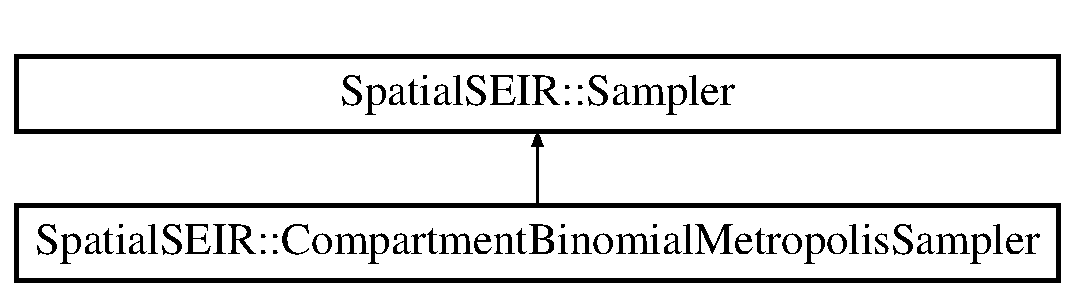
\includegraphics[height=2.000000cm]{classSpatialSEIR_1_1CompartmentBinomialMetropolisSampler}
\end{center}
\end{figure}
\subsection*{Public Member Functions}
\begin{DoxyCompactItemize}
\item 
\hyperlink{classSpatialSEIR_1_1CompartmentBinomialMetropolisSampler_a8098fe4333db437ebd754d67040fc758}{Compartment\-Binomial\-Metropolis\-Sampler} (\hyperlink{classSpatialSEIR_1_1ModelContext}{Model\-Context} $\ast$\hyperlink{classSpatialSEIR_1_1CompartmentBinomialMetropolisSampler_aa8e8332272c23e296ff8f3f6d9b6b9a2}{context}, \hyperlink{classSpatialSEIR_1_1CompartmentFullConditional}{Compartment\-Full\-Conditional} $\ast$\hyperlink{classSpatialSEIR_1_1CompartmentBinomialMetropolisSampler_a5ba83648853edd9ccf7e0e33e22b1d93}{compartment\-F\-C}, int $\ast$\hyperlink{classSpatialSEIR_1_1CompartmentBinomialMetropolisSampler_a05f080ab0846309ba240b1819249cb9c}{compartment\-Data}, int $\ast$\hyperlink{classSpatialSEIR_1_1CompartmentBinomialMetropolisSampler_a2927a09c8c50447fe863506c1e6e1a10}{compartment\-From}, int $\ast$\hyperlink{classSpatialSEIR_1_1CompartmentBinomialMetropolisSampler_a4b6410cc9b98d13ef261497292ba6518}{compartment\-To}, double $\ast$\hyperlink{classSpatialSEIR_1_1CompartmentBinomialMetropolisSampler_a6a93966308715d47f53c972b5f7e385b}{probability\-Vector}, int \hyperlink{classSpatialSEIR_1_1CompartmentBinomialMetropolisSampler_adad677ace3b19726b377834fcd78b857}{probability\-Vector\-Len})
\item 
void \hyperlink{classSpatialSEIR_1_1CompartmentBinomialMetropolisSampler_a11d2900ff89a59f71e2ff5695432e036}{draw\-Sample} ()
\item 
int \hyperlink{classSpatialSEIR_1_1CompartmentBinomialMetropolisSampler_aa84f51d4d02943be01c6309581ecc17a}{get\-Sampler\-Type} ()
\item 
void \hyperlink{classSpatialSEIR_1_1CompartmentBinomialMetropolisSampler_a3ba10e64272f38123df2963e9d52cdab}{gen\-Proposal} ()
\item 
\hyperlink{classSpatialSEIR_1_1CompartmentBinomialMetropolisSampler_aae485cd96f34f762416337db11da1f54}{$\sim$\-Compartment\-Binomial\-Metropolis\-Sampler} ()
\end{DoxyCompactItemize}
\subsection*{Public Attributes}
\begin{DoxyCompactItemize}
\item 
\hyperlink{classSpatialSEIR_1_1ModelContext}{Model\-Context} $\ast$$\ast$ \hyperlink{classSpatialSEIR_1_1CompartmentBinomialMetropolisSampler_aa8e8332272c23e296ff8f3f6d9b6b9a2}{context}
\item 
\hyperlink{classSpatialSEIR_1_1CompartmentFullConditional}{Compartment\-Full\-Conditional} $\ast$$\ast$ \hyperlink{classSpatialSEIR_1_1CompartmentBinomialMetropolisSampler_a5ba83648853edd9ccf7e0e33e22b1d93}{compartment\-F\-C}
\item 
int $\ast$$\ast$ \hyperlink{classSpatialSEIR_1_1CompartmentBinomialMetropolisSampler_a05f080ab0846309ba240b1819249cb9c}{compartment\-Data}
\item 
int $\ast$$\ast$ \hyperlink{classSpatialSEIR_1_1CompartmentBinomialMetropolisSampler_a2927a09c8c50447fe863506c1e6e1a10}{compartment\-From}
\item 
int $\ast$$\ast$ \hyperlink{classSpatialSEIR_1_1CompartmentBinomialMetropolisSampler_a4b6410cc9b98d13ef261497292ba6518}{compartment\-To}
\item 
double $\ast$$\ast$ \hyperlink{classSpatialSEIR_1_1CompartmentBinomialMetropolisSampler_a6a93966308715d47f53c972b5f7e385b}{probability\-Vector}
\item 
int $\ast$ \hyperlink{classSpatialSEIR_1_1CompartmentBinomialMetropolisSampler_adad677ace3b19726b377834fcd78b857}{probability\-Vector\-Len}
\end{DoxyCompactItemize}


\subsection{Detailed Description}
The \hyperlink{classSpatialSEIR_1_1CompartmentBinomialMetropolisSampler}{Compartment\-Binomial\-Metropolis\-Sampler} class is child of the \hyperlink{classSpatialSEIR_1_1Sampler}{Sampler} class which draws samples from the posterior distribution of the various transition compartments using a chain binomial proposal based on the parameters. 

\subsection{Constructor \& Destructor Documentation}
\hypertarget{classSpatialSEIR_1_1CompartmentBinomialMetropolisSampler_a8098fe4333db437ebd754d67040fc758}{\index{Spatial\-S\-E\-I\-R\-::\-Compartment\-Binomial\-Metropolis\-Sampler@{Spatial\-S\-E\-I\-R\-::\-Compartment\-Binomial\-Metropolis\-Sampler}!Compartment\-Binomial\-Metropolis\-Sampler@{Compartment\-Binomial\-Metropolis\-Sampler}}
\index{Compartment\-Binomial\-Metropolis\-Sampler@{Compartment\-Binomial\-Metropolis\-Sampler}!SpatialSEIR::CompartmentBinomialMetropolisSampler@{Spatial\-S\-E\-I\-R\-::\-Compartment\-Binomial\-Metropolis\-Sampler}}
\subsubsection[{Compartment\-Binomial\-Metropolis\-Sampler}]{\setlength{\rightskip}{0pt plus 5cm}Spatial\-S\-E\-I\-R\-::\-Compartment\-Binomial\-Metropolis\-Sampler\-::\-Compartment\-Binomial\-Metropolis\-Sampler (
\begin{DoxyParamCaption}
\item[{{\bf Model\-Context} $\ast$}]{context, }
\item[{{\bf Compartment\-Full\-Conditional} $\ast$}]{compartment\-F\-C, }
\item[{int $\ast$}]{compartment\-Data, }
\item[{int $\ast$}]{compartment\-From, }
\item[{int $\ast$}]{compartment\-To, }
\item[{double $\ast$}]{probability\-Vector, }
\item[{int}]{probability\-Vector\-Len}
\end{DoxyParamCaption}
)}}\label{classSpatialSEIR_1_1CompartmentBinomialMetropolisSampler_a8098fe4333db437ebd754d67040fc758}
\hypertarget{classSpatialSEIR_1_1CompartmentBinomialMetropolisSampler_aae485cd96f34f762416337db11da1f54}{\index{Spatial\-S\-E\-I\-R\-::\-Compartment\-Binomial\-Metropolis\-Sampler@{Spatial\-S\-E\-I\-R\-::\-Compartment\-Binomial\-Metropolis\-Sampler}!$\sim$\-Compartment\-Binomial\-Metropolis\-Sampler@{$\sim$\-Compartment\-Binomial\-Metropolis\-Sampler}}
\index{$\sim$\-Compartment\-Binomial\-Metropolis\-Sampler@{$\sim$\-Compartment\-Binomial\-Metropolis\-Sampler}!SpatialSEIR::CompartmentBinomialMetropolisSampler@{Spatial\-S\-E\-I\-R\-::\-Compartment\-Binomial\-Metropolis\-Sampler}}
\subsubsection[{$\sim$\-Compartment\-Binomial\-Metropolis\-Sampler}]{\setlength{\rightskip}{0pt plus 5cm}Spatial\-S\-E\-I\-R\-::\-Compartment\-Binomial\-Metropolis\-Sampler\-::$\sim$\-Compartment\-Binomial\-Metropolis\-Sampler (
\begin{DoxyParamCaption}
{}
\end{DoxyParamCaption}
)}}\label{classSpatialSEIR_1_1CompartmentBinomialMetropolisSampler_aae485cd96f34f762416337db11da1f54}


\subsection{Member Function Documentation}
\hypertarget{classSpatialSEIR_1_1CompartmentBinomialMetropolisSampler_a11d2900ff89a59f71e2ff5695432e036}{\index{Spatial\-S\-E\-I\-R\-::\-Compartment\-Binomial\-Metropolis\-Sampler@{Spatial\-S\-E\-I\-R\-::\-Compartment\-Binomial\-Metropolis\-Sampler}!draw\-Sample@{draw\-Sample}}
\index{draw\-Sample@{draw\-Sample}!SpatialSEIR::CompartmentBinomialMetropolisSampler@{Spatial\-S\-E\-I\-R\-::\-Compartment\-Binomial\-Metropolis\-Sampler}}
\subsubsection[{draw\-Sample}]{\setlength{\rightskip}{0pt plus 5cm}void Spatial\-S\-E\-I\-R\-::\-Compartment\-Binomial\-Metropolis\-Sampler\-::draw\-Sample (
\begin{DoxyParamCaption}
{}
\end{DoxyParamCaption}
)\hspace{0.3cm}{\ttfamily [virtual]}}}\label{classSpatialSEIR_1_1CompartmentBinomialMetropolisSampler_a11d2900ff89a59f71e2ff5695432e036}


Implements \hyperlink{classSpatialSEIR_1_1Sampler_aa07a42b26cb62249c20c58e855a08657}{Spatial\-S\-E\-I\-R\-::\-Sampler}.

\hypertarget{classSpatialSEIR_1_1CompartmentBinomialMetropolisSampler_a3ba10e64272f38123df2963e9d52cdab}{\index{Spatial\-S\-E\-I\-R\-::\-Compartment\-Binomial\-Metropolis\-Sampler@{Spatial\-S\-E\-I\-R\-::\-Compartment\-Binomial\-Metropolis\-Sampler}!gen\-Proposal@{gen\-Proposal}}
\index{gen\-Proposal@{gen\-Proposal}!SpatialSEIR::CompartmentBinomialMetropolisSampler@{Spatial\-S\-E\-I\-R\-::\-Compartment\-Binomial\-Metropolis\-Sampler}}
\subsubsection[{gen\-Proposal}]{\setlength{\rightskip}{0pt plus 5cm}void Spatial\-S\-E\-I\-R\-::\-Compartment\-Binomial\-Metropolis\-Sampler\-::gen\-Proposal (
\begin{DoxyParamCaption}
{}
\end{DoxyParamCaption}
)}}\label{classSpatialSEIR_1_1CompartmentBinomialMetropolisSampler_a3ba10e64272f38123df2963e9d52cdab}
\hypertarget{classSpatialSEIR_1_1CompartmentBinomialMetropolisSampler_aa84f51d4d02943be01c6309581ecc17a}{\index{Spatial\-S\-E\-I\-R\-::\-Compartment\-Binomial\-Metropolis\-Sampler@{Spatial\-S\-E\-I\-R\-::\-Compartment\-Binomial\-Metropolis\-Sampler}!get\-Sampler\-Type@{get\-Sampler\-Type}}
\index{get\-Sampler\-Type@{get\-Sampler\-Type}!SpatialSEIR::CompartmentBinomialMetropolisSampler@{Spatial\-S\-E\-I\-R\-::\-Compartment\-Binomial\-Metropolis\-Sampler}}
\subsubsection[{get\-Sampler\-Type}]{\setlength{\rightskip}{0pt plus 5cm}int Spatial\-S\-E\-I\-R\-::\-Compartment\-Binomial\-Metropolis\-Sampler\-::get\-Sampler\-Type (
\begin{DoxyParamCaption}
{}
\end{DoxyParamCaption}
)\hspace{0.3cm}{\ttfamily [virtual]}}}\label{classSpatialSEIR_1_1CompartmentBinomialMetropolisSampler_aa84f51d4d02943be01c6309581ecc17a}


Implements \hyperlink{classSpatialSEIR_1_1Sampler_aaa79310ad809e6aeb25479849f322dda}{Spatial\-S\-E\-I\-R\-::\-Sampler}.



\subsection{Member Data Documentation}
\hypertarget{classSpatialSEIR_1_1CompartmentBinomialMetropolisSampler_a05f080ab0846309ba240b1819249cb9c}{\index{Spatial\-S\-E\-I\-R\-::\-Compartment\-Binomial\-Metropolis\-Sampler@{Spatial\-S\-E\-I\-R\-::\-Compartment\-Binomial\-Metropolis\-Sampler}!compartment\-Data@{compartment\-Data}}
\index{compartment\-Data@{compartment\-Data}!SpatialSEIR::CompartmentBinomialMetropolisSampler@{Spatial\-S\-E\-I\-R\-::\-Compartment\-Binomial\-Metropolis\-Sampler}}
\subsubsection[{compartment\-Data}]{\setlength{\rightskip}{0pt plus 5cm}int$\ast$$\ast$ Spatial\-S\-E\-I\-R\-::\-Compartment\-Binomial\-Metropolis\-Sampler\-::compartment\-Data}}\label{classSpatialSEIR_1_1CompartmentBinomialMetropolisSampler_a05f080ab0846309ba240b1819249cb9c}
\hypertarget{classSpatialSEIR_1_1CompartmentBinomialMetropolisSampler_a5ba83648853edd9ccf7e0e33e22b1d93}{\index{Spatial\-S\-E\-I\-R\-::\-Compartment\-Binomial\-Metropolis\-Sampler@{Spatial\-S\-E\-I\-R\-::\-Compartment\-Binomial\-Metropolis\-Sampler}!compartment\-F\-C@{compartment\-F\-C}}
\index{compartment\-F\-C@{compartment\-F\-C}!SpatialSEIR::CompartmentBinomialMetropolisSampler@{Spatial\-S\-E\-I\-R\-::\-Compartment\-Binomial\-Metropolis\-Sampler}}
\subsubsection[{compartment\-F\-C}]{\setlength{\rightskip}{0pt plus 5cm}{\bf Compartment\-Full\-Conditional}$\ast$$\ast$ Spatial\-S\-E\-I\-R\-::\-Compartment\-Binomial\-Metropolis\-Sampler\-::compartment\-F\-C}}\label{classSpatialSEIR_1_1CompartmentBinomialMetropolisSampler_a5ba83648853edd9ccf7e0e33e22b1d93}
\hypertarget{classSpatialSEIR_1_1CompartmentBinomialMetropolisSampler_a2927a09c8c50447fe863506c1e6e1a10}{\index{Spatial\-S\-E\-I\-R\-::\-Compartment\-Binomial\-Metropolis\-Sampler@{Spatial\-S\-E\-I\-R\-::\-Compartment\-Binomial\-Metropolis\-Sampler}!compartment\-From@{compartment\-From}}
\index{compartment\-From@{compartment\-From}!SpatialSEIR::CompartmentBinomialMetropolisSampler@{Spatial\-S\-E\-I\-R\-::\-Compartment\-Binomial\-Metropolis\-Sampler}}
\subsubsection[{compartment\-From}]{\setlength{\rightskip}{0pt plus 5cm}int$\ast$$\ast$ Spatial\-S\-E\-I\-R\-::\-Compartment\-Binomial\-Metropolis\-Sampler\-::compartment\-From}}\label{classSpatialSEIR_1_1CompartmentBinomialMetropolisSampler_a2927a09c8c50447fe863506c1e6e1a10}
\hypertarget{classSpatialSEIR_1_1CompartmentBinomialMetropolisSampler_a4b6410cc9b98d13ef261497292ba6518}{\index{Spatial\-S\-E\-I\-R\-::\-Compartment\-Binomial\-Metropolis\-Sampler@{Spatial\-S\-E\-I\-R\-::\-Compartment\-Binomial\-Metropolis\-Sampler}!compartment\-To@{compartment\-To}}
\index{compartment\-To@{compartment\-To}!SpatialSEIR::CompartmentBinomialMetropolisSampler@{Spatial\-S\-E\-I\-R\-::\-Compartment\-Binomial\-Metropolis\-Sampler}}
\subsubsection[{compartment\-To}]{\setlength{\rightskip}{0pt plus 5cm}int$\ast$$\ast$ Spatial\-S\-E\-I\-R\-::\-Compartment\-Binomial\-Metropolis\-Sampler\-::compartment\-To}}\label{classSpatialSEIR_1_1CompartmentBinomialMetropolisSampler_a4b6410cc9b98d13ef261497292ba6518}
\hypertarget{classSpatialSEIR_1_1CompartmentBinomialMetropolisSampler_aa8e8332272c23e296ff8f3f6d9b6b9a2}{\index{Spatial\-S\-E\-I\-R\-::\-Compartment\-Binomial\-Metropolis\-Sampler@{Spatial\-S\-E\-I\-R\-::\-Compartment\-Binomial\-Metropolis\-Sampler}!context@{context}}
\index{context@{context}!SpatialSEIR::CompartmentBinomialMetropolisSampler@{Spatial\-S\-E\-I\-R\-::\-Compartment\-Binomial\-Metropolis\-Sampler}}
\subsubsection[{context}]{\setlength{\rightskip}{0pt plus 5cm}{\bf Model\-Context}$\ast$$\ast$ Spatial\-S\-E\-I\-R\-::\-Compartment\-Binomial\-Metropolis\-Sampler\-::context}}\label{classSpatialSEIR_1_1CompartmentBinomialMetropolisSampler_aa8e8332272c23e296ff8f3f6d9b6b9a2}
\hypertarget{classSpatialSEIR_1_1CompartmentBinomialMetropolisSampler_a6a93966308715d47f53c972b5f7e385b}{\index{Spatial\-S\-E\-I\-R\-::\-Compartment\-Binomial\-Metropolis\-Sampler@{Spatial\-S\-E\-I\-R\-::\-Compartment\-Binomial\-Metropolis\-Sampler}!probability\-Vector@{probability\-Vector}}
\index{probability\-Vector@{probability\-Vector}!SpatialSEIR::CompartmentBinomialMetropolisSampler@{Spatial\-S\-E\-I\-R\-::\-Compartment\-Binomial\-Metropolis\-Sampler}}
\subsubsection[{probability\-Vector}]{\setlength{\rightskip}{0pt plus 5cm}double$\ast$$\ast$ Spatial\-S\-E\-I\-R\-::\-Compartment\-Binomial\-Metropolis\-Sampler\-::probability\-Vector}}\label{classSpatialSEIR_1_1CompartmentBinomialMetropolisSampler_a6a93966308715d47f53c972b5f7e385b}
\hypertarget{classSpatialSEIR_1_1CompartmentBinomialMetropolisSampler_adad677ace3b19726b377834fcd78b857}{\index{Spatial\-S\-E\-I\-R\-::\-Compartment\-Binomial\-Metropolis\-Sampler@{Spatial\-S\-E\-I\-R\-::\-Compartment\-Binomial\-Metropolis\-Sampler}!probability\-Vector\-Len@{probability\-Vector\-Len}}
\index{probability\-Vector\-Len@{probability\-Vector\-Len}!SpatialSEIR::CompartmentBinomialMetropolisSampler@{Spatial\-S\-E\-I\-R\-::\-Compartment\-Binomial\-Metropolis\-Sampler}}
\subsubsection[{probability\-Vector\-Len}]{\setlength{\rightskip}{0pt plus 5cm}int$\ast$ Spatial\-S\-E\-I\-R\-::\-Compartment\-Binomial\-Metropolis\-Sampler\-::probability\-Vector\-Len}}\label{classSpatialSEIR_1_1CompartmentBinomialMetropolisSampler_adad677ace3b19726b377834fcd78b857}


The documentation for this class was generated from the following file\-:\begin{DoxyCompactItemize}
\item 
lib\-Spatial\-S\-E\-I\-R/include/\hyperlink{LSS__Samplers_8hpp}{L\-S\-S\-\_\-\-Samplers.\-hpp}\end{DoxyCompactItemize}

\hypertarget{classSpatialSEIR_1_1CompartmentBinomialSliceSampler}{\section{Spatial\-S\-E\-I\-R\-:\-:Compartment\-Binomial\-Slice\-Sampler Class Reference}
\label{classSpatialSEIR_1_1CompartmentBinomialSliceSampler}\index{Spatial\-S\-E\-I\-R\-::\-Compartment\-Binomial\-Slice\-Sampler@{Spatial\-S\-E\-I\-R\-::\-Compartment\-Binomial\-Slice\-Sampler}}
}


{\ttfamily \#include $<$L\-S\-S\-\_\-\-Samplers.\-hpp$>$}

Inheritance diagram for Spatial\-S\-E\-I\-R\-:\-:Compartment\-Binomial\-Slice\-Sampler\-:\begin{figure}[H]
\begin{center}
\leavevmode
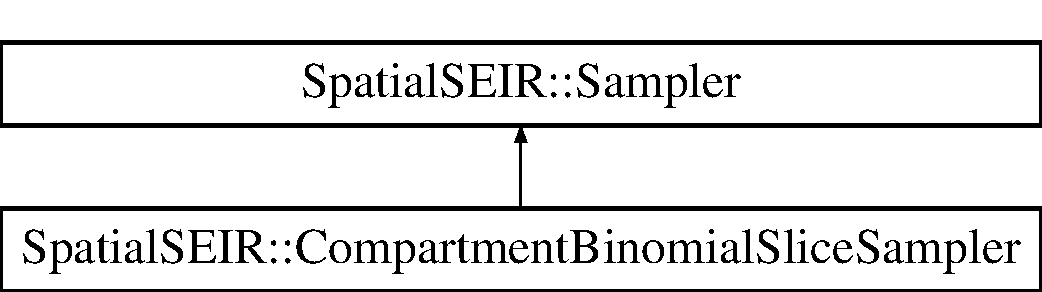
\includegraphics[height=2.000000cm]{classSpatialSEIR_1_1CompartmentBinomialSliceSampler}
\end{center}
\end{figure}
\subsection*{Public Member Functions}
\begin{DoxyCompactItemize}
\item 
\hyperlink{classSpatialSEIR_1_1CompartmentBinomialSliceSampler_a9ebfe2b2d471f4bcc8dff23cd23685fa}{Compartment\-Binomial\-Slice\-Sampler} (\hyperlink{classSpatialSEIR_1_1ModelContext}{Model\-Context} $\ast$\hyperlink{classSpatialSEIR_1_1CompartmentBinomialSliceSampler_ad5631c8afe2fe4d0e8563b72fae517b0}{context}, \hyperlink{classSpatialSEIR_1_1CompartmentFullConditional}{Compartment\-Full\-Conditional} $\ast$\hyperlink{classSpatialSEIR_1_1CompartmentBinomialSliceSampler_abd146e1a97514494297f7863a61d381d}{compartment\-F\-C}, int $\ast$\hyperlink{classSpatialSEIR_1_1CompartmentBinomialSliceSampler_a6094cf1e5d3773db4d89186f19507c99}{compartment\-Data}, int $\ast$\hyperlink{classSpatialSEIR_1_1CompartmentBinomialSliceSampler_a7a8d30fa7485e4db0e68faa38aa7bc61}{compartment\-From}, int $\ast$\hyperlink{classSpatialSEIR_1_1CompartmentBinomialSliceSampler_a51e5687941d0911f0c5760af847b9c5d}{compartment\-To}, double $\ast$\hyperlink{classSpatialSEIR_1_1CompartmentBinomialSliceSampler_aff766a8c61753ae89e8b1a6ffea0d108}{probability\-Vector}, int \hyperlink{classSpatialSEIR_1_1CompartmentBinomialSliceSampler_aac982be0c3ae19b0a9960c0dbd1107ac}{probability\-Vector\-Len})
\item 
void \hyperlink{classSpatialSEIR_1_1CompartmentBinomialSliceSampler_a6d89f57c350e131068718374ae0d135f}{draw\-Sample} ()
\item 
int \hyperlink{classSpatialSEIR_1_1CompartmentBinomialSliceSampler_a35f2ba8531217f1fa227da3b801d05dd}{get\-Sampler\-Type} ()
\item 
void \hyperlink{classSpatialSEIR_1_1CompartmentBinomialSliceSampler_a231c0b5e4334099ef663ad5d59809ded}{gen\-Proposal} ()
\item 
\hyperlink{classSpatialSEIR_1_1CompartmentBinomialSliceSampler_af0661567a3b84368cf8c5e64a6f4fc3e}{$\sim$\-Compartment\-Binomial\-Slice\-Sampler} ()
\end{DoxyCompactItemize}
\subsection*{Public Attributes}
\begin{DoxyCompactItemize}
\item 
\hyperlink{classSpatialSEIR_1_1ModelContext}{Model\-Context} $\ast$$\ast$ \hyperlink{classSpatialSEIR_1_1CompartmentBinomialSliceSampler_ad5631c8afe2fe4d0e8563b72fae517b0}{context}
\item 
\hyperlink{classSpatialSEIR_1_1CompartmentFullConditional}{Compartment\-Full\-Conditional} $\ast$$\ast$ \hyperlink{classSpatialSEIR_1_1CompartmentBinomialSliceSampler_abd146e1a97514494297f7863a61d381d}{compartment\-F\-C}
\item 
int $\ast$$\ast$ \hyperlink{classSpatialSEIR_1_1CompartmentBinomialSliceSampler_a6094cf1e5d3773db4d89186f19507c99}{compartment\-Data}
\item 
int $\ast$$\ast$ \hyperlink{classSpatialSEIR_1_1CompartmentBinomialSliceSampler_a7a8d30fa7485e4db0e68faa38aa7bc61}{compartment\-From}
\item 
int $\ast$$\ast$ \hyperlink{classSpatialSEIR_1_1CompartmentBinomialSliceSampler_a51e5687941d0911f0c5760af847b9c5d}{compartment\-To}
\item 
double $\ast$$\ast$ \hyperlink{classSpatialSEIR_1_1CompartmentBinomialSliceSampler_aff766a8c61753ae89e8b1a6ffea0d108}{probability\-Vector}
\item 
int $\ast$ \hyperlink{classSpatialSEIR_1_1CompartmentBinomialSliceSampler_aac982be0c3ae19b0a9960c0dbd1107ac}{probability\-Vector\-Len}
\end{DoxyCompactItemize}


\subsection{Detailed Description}
The \hyperlink{classSpatialSEIR_1_1CompartmentBinomialSliceSampler}{Compartment\-Binomial\-Slice\-Sampler} class is child of the \hyperlink{classSpatialSEIR_1_1Sampler}{Sampler} class which draws samples from the posterior distribution of the various transition compartments using a chain binomial proposal based on the parameters. 

\subsection{Constructor \& Destructor Documentation}
\hypertarget{classSpatialSEIR_1_1CompartmentBinomialSliceSampler_a9ebfe2b2d471f4bcc8dff23cd23685fa}{\index{Spatial\-S\-E\-I\-R\-::\-Compartment\-Binomial\-Slice\-Sampler@{Spatial\-S\-E\-I\-R\-::\-Compartment\-Binomial\-Slice\-Sampler}!Compartment\-Binomial\-Slice\-Sampler@{Compartment\-Binomial\-Slice\-Sampler}}
\index{Compartment\-Binomial\-Slice\-Sampler@{Compartment\-Binomial\-Slice\-Sampler}!SpatialSEIR::CompartmentBinomialSliceSampler@{Spatial\-S\-E\-I\-R\-::\-Compartment\-Binomial\-Slice\-Sampler}}
\subsubsection[{Compartment\-Binomial\-Slice\-Sampler}]{\setlength{\rightskip}{0pt plus 5cm}Spatial\-S\-E\-I\-R\-::\-Compartment\-Binomial\-Slice\-Sampler\-::\-Compartment\-Binomial\-Slice\-Sampler (
\begin{DoxyParamCaption}
\item[{{\bf Model\-Context} $\ast$}]{context, }
\item[{{\bf Compartment\-Full\-Conditional} $\ast$}]{compartment\-F\-C, }
\item[{int $\ast$}]{compartment\-Data, }
\item[{int $\ast$}]{compartment\-From, }
\item[{int $\ast$}]{compartment\-To, }
\item[{double $\ast$}]{probability\-Vector, }
\item[{int}]{probability\-Vector\-Len}
\end{DoxyParamCaption}
)}}\label{classSpatialSEIR_1_1CompartmentBinomialSliceSampler_a9ebfe2b2d471f4bcc8dff23cd23685fa}
\hypertarget{classSpatialSEIR_1_1CompartmentBinomialSliceSampler_af0661567a3b84368cf8c5e64a6f4fc3e}{\index{Spatial\-S\-E\-I\-R\-::\-Compartment\-Binomial\-Slice\-Sampler@{Spatial\-S\-E\-I\-R\-::\-Compartment\-Binomial\-Slice\-Sampler}!$\sim$\-Compartment\-Binomial\-Slice\-Sampler@{$\sim$\-Compartment\-Binomial\-Slice\-Sampler}}
\index{$\sim$\-Compartment\-Binomial\-Slice\-Sampler@{$\sim$\-Compartment\-Binomial\-Slice\-Sampler}!SpatialSEIR::CompartmentBinomialSliceSampler@{Spatial\-S\-E\-I\-R\-::\-Compartment\-Binomial\-Slice\-Sampler}}
\subsubsection[{$\sim$\-Compartment\-Binomial\-Slice\-Sampler}]{\setlength{\rightskip}{0pt plus 5cm}Spatial\-S\-E\-I\-R\-::\-Compartment\-Binomial\-Slice\-Sampler\-::$\sim$\-Compartment\-Binomial\-Slice\-Sampler (
\begin{DoxyParamCaption}
{}
\end{DoxyParamCaption}
)}}\label{classSpatialSEIR_1_1CompartmentBinomialSliceSampler_af0661567a3b84368cf8c5e64a6f4fc3e}


\subsection{Member Function Documentation}
\hypertarget{classSpatialSEIR_1_1CompartmentBinomialSliceSampler_a6d89f57c350e131068718374ae0d135f}{\index{Spatial\-S\-E\-I\-R\-::\-Compartment\-Binomial\-Slice\-Sampler@{Spatial\-S\-E\-I\-R\-::\-Compartment\-Binomial\-Slice\-Sampler}!draw\-Sample@{draw\-Sample}}
\index{draw\-Sample@{draw\-Sample}!SpatialSEIR::CompartmentBinomialSliceSampler@{Spatial\-S\-E\-I\-R\-::\-Compartment\-Binomial\-Slice\-Sampler}}
\subsubsection[{draw\-Sample}]{\setlength{\rightskip}{0pt plus 5cm}void Spatial\-S\-E\-I\-R\-::\-Compartment\-Binomial\-Slice\-Sampler\-::draw\-Sample (
\begin{DoxyParamCaption}
{}
\end{DoxyParamCaption}
)\hspace{0.3cm}{\ttfamily [virtual]}}}\label{classSpatialSEIR_1_1CompartmentBinomialSliceSampler_a6d89f57c350e131068718374ae0d135f}


Implements \hyperlink{classSpatialSEIR_1_1Sampler_aa07a42b26cb62249c20c58e855a08657}{Spatial\-S\-E\-I\-R\-::\-Sampler}.

\hypertarget{classSpatialSEIR_1_1CompartmentBinomialSliceSampler_a231c0b5e4334099ef663ad5d59809ded}{\index{Spatial\-S\-E\-I\-R\-::\-Compartment\-Binomial\-Slice\-Sampler@{Spatial\-S\-E\-I\-R\-::\-Compartment\-Binomial\-Slice\-Sampler}!gen\-Proposal@{gen\-Proposal}}
\index{gen\-Proposal@{gen\-Proposal}!SpatialSEIR::CompartmentBinomialSliceSampler@{Spatial\-S\-E\-I\-R\-::\-Compartment\-Binomial\-Slice\-Sampler}}
\subsubsection[{gen\-Proposal}]{\setlength{\rightskip}{0pt plus 5cm}void Spatial\-S\-E\-I\-R\-::\-Compartment\-Binomial\-Slice\-Sampler\-::gen\-Proposal (
\begin{DoxyParamCaption}
{}
\end{DoxyParamCaption}
)}}\label{classSpatialSEIR_1_1CompartmentBinomialSliceSampler_a231c0b5e4334099ef663ad5d59809ded}
\hypertarget{classSpatialSEIR_1_1CompartmentBinomialSliceSampler_a35f2ba8531217f1fa227da3b801d05dd}{\index{Spatial\-S\-E\-I\-R\-::\-Compartment\-Binomial\-Slice\-Sampler@{Spatial\-S\-E\-I\-R\-::\-Compartment\-Binomial\-Slice\-Sampler}!get\-Sampler\-Type@{get\-Sampler\-Type}}
\index{get\-Sampler\-Type@{get\-Sampler\-Type}!SpatialSEIR::CompartmentBinomialSliceSampler@{Spatial\-S\-E\-I\-R\-::\-Compartment\-Binomial\-Slice\-Sampler}}
\subsubsection[{get\-Sampler\-Type}]{\setlength{\rightskip}{0pt plus 5cm}int Spatial\-S\-E\-I\-R\-::\-Compartment\-Binomial\-Slice\-Sampler\-::get\-Sampler\-Type (
\begin{DoxyParamCaption}
{}
\end{DoxyParamCaption}
)\hspace{0.3cm}{\ttfamily [virtual]}}}\label{classSpatialSEIR_1_1CompartmentBinomialSliceSampler_a35f2ba8531217f1fa227da3b801d05dd}


Implements \hyperlink{classSpatialSEIR_1_1Sampler_aaa79310ad809e6aeb25479849f322dda}{Spatial\-S\-E\-I\-R\-::\-Sampler}.



\subsection{Member Data Documentation}
\hypertarget{classSpatialSEIR_1_1CompartmentBinomialSliceSampler_a6094cf1e5d3773db4d89186f19507c99}{\index{Spatial\-S\-E\-I\-R\-::\-Compartment\-Binomial\-Slice\-Sampler@{Spatial\-S\-E\-I\-R\-::\-Compartment\-Binomial\-Slice\-Sampler}!compartment\-Data@{compartment\-Data}}
\index{compartment\-Data@{compartment\-Data}!SpatialSEIR::CompartmentBinomialSliceSampler@{Spatial\-S\-E\-I\-R\-::\-Compartment\-Binomial\-Slice\-Sampler}}
\subsubsection[{compartment\-Data}]{\setlength{\rightskip}{0pt plus 5cm}int$\ast$$\ast$ Spatial\-S\-E\-I\-R\-::\-Compartment\-Binomial\-Slice\-Sampler\-::compartment\-Data}}\label{classSpatialSEIR_1_1CompartmentBinomialSliceSampler_a6094cf1e5d3773db4d89186f19507c99}
\hypertarget{classSpatialSEIR_1_1CompartmentBinomialSliceSampler_abd146e1a97514494297f7863a61d381d}{\index{Spatial\-S\-E\-I\-R\-::\-Compartment\-Binomial\-Slice\-Sampler@{Spatial\-S\-E\-I\-R\-::\-Compartment\-Binomial\-Slice\-Sampler}!compartment\-F\-C@{compartment\-F\-C}}
\index{compartment\-F\-C@{compartment\-F\-C}!SpatialSEIR::CompartmentBinomialSliceSampler@{Spatial\-S\-E\-I\-R\-::\-Compartment\-Binomial\-Slice\-Sampler}}
\subsubsection[{compartment\-F\-C}]{\setlength{\rightskip}{0pt plus 5cm}{\bf Compartment\-Full\-Conditional}$\ast$$\ast$ Spatial\-S\-E\-I\-R\-::\-Compartment\-Binomial\-Slice\-Sampler\-::compartment\-F\-C}}\label{classSpatialSEIR_1_1CompartmentBinomialSliceSampler_abd146e1a97514494297f7863a61d381d}
\hypertarget{classSpatialSEIR_1_1CompartmentBinomialSliceSampler_a7a8d30fa7485e4db0e68faa38aa7bc61}{\index{Spatial\-S\-E\-I\-R\-::\-Compartment\-Binomial\-Slice\-Sampler@{Spatial\-S\-E\-I\-R\-::\-Compartment\-Binomial\-Slice\-Sampler}!compartment\-From@{compartment\-From}}
\index{compartment\-From@{compartment\-From}!SpatialSEIR::CompartmentBinomialSliceSampler@{Spatial\-S\-E\-I\-R\-::\-Compartment\-Binomial\-Slice\-Sampler}}
\subsubsection[{compartment\-From}]{\setlength{\rightskip}{0pt plus 5cm}int$\ast$$\ast$ Spatial\-S\-E\-I\-R\-::\-Compartment\-Binomial\-Slice\-Sampler\-::compartment\-From}}\label{classSpatialSEIR_1_1CompartmentBinomialSliceSampler_a7a8d30fa7485e4db0e68faa38aa7bc61}
\hypertarget{classSpatialSEIR_1_1CompartmentBinomialSliceSampler_a51e5687941d0911f0c5760af847b9c5d}{\index{Spatial\-S\-E\-I\-R\-::\-Compartment\-Binomial\-Slice\-Sampler@{Spatial\-S\-E\-I\-R\-::\-Compartment\-Binomial\-Slice\-Sampler}!compartment\-To@{compartment\-To}}
\index{compartment\-To@{compartment\-To}!SpatialSEIR::CompartmentBinomialSliceSampler@{Spatial\-S\-E\-I\-R\-::\-Compartment\-Binomial\-Slice\-Sampler}}
\subsubsection[{compartment\-To}]{\setlength{\rightskip}{0pt plus 5cm}int$\ast$$\ast$ Spatial\-S\-E\-I\-R\-::\-Compartment\-Binomial\-Slice\-Sampler\-::compartment\-To}}\label{classSpatialSEIR_1_1CompartmentBinomialSliceSampler_a51e5687941d0911f0c5760af847b9c5d}
\hypertarget{classSpatialSEIR_1_1CompartmentBinomialSliceSampler_ad5631c8afe2fe4d0e8563b72fae517b0}{\index{Spatial\-S\-E\-I\-R\-::\-Compartment\-Binomial\-Slice\-Sampler@{Spatial\-S\-E\-I\-R\-::\-Compartment\-Binomial\-Slice\-Sampler}!context@{context}}
\index{context@{context}!SpatialSEIR::CompartmentBinomialSliceSampler@{Spatial\-S\-E\-I\-R\-::\-Compartment\-Binomial\-Slice\-Sampler}}
\subsubsection[{context}]{\setlength{\rightskip}{0pt plus 5cm}{\bf Model\-Context}$\ast$$\ast$ Spatial\-S\-E\-I\-R\-::\-Compartment\-Binomial\-Slice\-Sampler\-::context}}\label{classSpatialSEIR_1_1CompartmentBinomialSliceSampler_ad5631c8afe2fe4d0e8563b72fae517b0}
\hypertarget{classSpatialSEIR_1_1CompartmentBinomialSliceSampler_aff766a8c61753ae89e8b1a6ffea0d108}{\index{Spatial\-S\-E\-I\-R\-::\-Compartment\-Binomial\-Slice\-Sampler@{Spatial\-S\-E\-I\-R\-::\-Compartment\-Binomial\-Slice\-Sampler}!probability\-Vector@{probability\-Vector}}
\index{probability\-Vector@{probability\-Vector}!SpatialSEIR::CompartmentBinomialSliceSampler@{Spatial\-S\-E\-I\-R\-::\-Compartment\-Binomial\-Slice\-Sampler}}
\subsubsection[{probability\-Vector}]{\setlength{\rightskip}{0pt plus 5cm}double$\ast$$\ast$ Spatial\-S\-E\-I\-R\-::\-Compartment\-Binomial\-Slice\-Sampler\-::probability\-Vector}}\label{classSpatialSEIR_1_1CompartmentBinomialSliceSampler_aff766a8c61753ae89e8b1a6ffea0d108}
\hypertarget{classSpatialSEIR_1_1CompartmentBinomialSliceSampler_aac982be0c3ae19b0a9960c0dbd1107ac}{\index{Spatial\-S\-E\-I\-R\-::\-Compartment\-Binomial\-Slice\-Sampler@{Spatial\-S\-E\-I\-R\-::\-Compartment\-Binomial\-Slice\-Sampler}!probability\-Vector\-Len@{probability\-Vector\-Len}}
\index{probability\-Vector\-Len@{probability\-Vector\-Len}!SpatialSEIR::CompartmentBinomialSliceSampler@{Spatial\-S\-E\-I\-R\-::\-Compartment\-Binomial\-Slice\-Sampler}}
\subsubsection[{probability\-Vector\-Len}]{\setlength{\rightskip}{0pt plus 5cm}int$\ast$ Spatial\-S\-E\-I\-R\-::\-Compartment\-Binomial\-Slice\-Sampler\-::probability\-Vector\-Len}}\label{classSpatialSEIR_1_1CompartmentBinomialSliceSampler_aac982be0c3ae19b0a9960c0dbd1107ac}


The documentation for this class was generated from the following file\-:\begin{DoxyCompactItemize}
\item 
lib\-Spatial\-S\-E\-I\-R/include/\hyperlink{LSS__Samplers_8hpp}{L\-S\-S\-\_\-\-Samplers.\-hpp}\end{DoxyCompactItemize}

\hypertarget{classSpatialSEIR_1_1CompartmentFullConditional}{\section{Spatial\-S\-E\-I\-R\-:\-:Compartment\-Full\-Conditional Class Reference}
\label{classSpatialSEIR_1_1CompartmentFullConditional}\index{Spatial\-S\-E\-I\-R\-::\-Compartment\-Full\-Conditional@{Spatial\-S\-E\-I\-R\-::\-Compartment\-Full\-Conditional}}
}


{\ttfamily \#include $<$L\-S\-S\-\_\-\-Full\-Conditional.\-hpp$>$}

Inheritance diagram for Spatial\-S\-E\-I\-R\-:\-:Compartment\-Full\-Conditional\-:\begin{figure}[H]
\begin{center}
\leavevmode
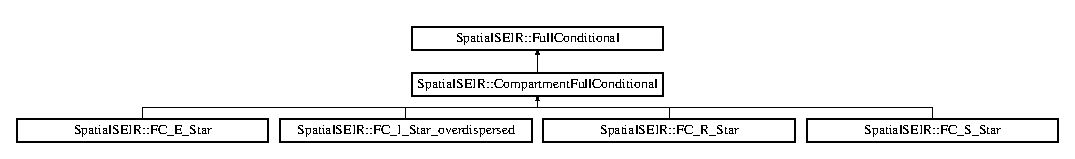
\includegraphics[height=1.693548cm]{classSpatialSEIR_1_1CompartmentFullConditional}
\end{center}
\end{figure}
\subsection*{Public Member Functions}
\begin{DoxyCompactItemize}
\item 
virtual \hyperlink{classSpatialSEIR_1_1CompartmentFullConditional_a7dd59bdf5663913955fb61573e7a5f1f}{$\sim$\-Compartment\-Full\-Conditional} ()
\item 
virtual int \hyperlink{classSpatialSEIR_1_1CompartmentFullConditional_ad2402c8d7fc0b362482bcd5ceaa035af}{eval\-C\-P\-U} ()=0
\item 
virtual int \hyperlink{classSpatialSEIR_1_1CompartmentFullConditional_a92d48bc8cd13ff048791edbdcc453479}{eval\-C\-P\-U} (int i, int j)=0
\item 
virtual int \hyperlink{classSpatialSEIR_1_1CompartmentFullConditional_ac7c7b1191508d49a56ec739449bf93d4}{eval\-O\-C\-L} ()=0
\item 
virtual void \hyperlink{classSpatialSEIR_1_1CompartmentFullConditional_a436ae9e47f7a4269f0a78ce225e6b7f3}{sample} (int verbose)=0
\item 
virtual long double \hyperlink{classSpatialSEIR_1_1CompartmentFullConditional_a28794be23ee7f6fcba96ff2bee63e065}{get\-Value} ()=0
\item 
virtual void \hyperlink{classSpatialSEIR_1_1CompartmentFullConditional_a22ab4dcc354c8ebc4f619685bc32dfae}{set\-Value} (long double value)=0
\item 
virtual int \hyperlink{classSpatialSEIR_1_1CompartmentFullConditional_a71836271b0997117f3b8437c2f55a986}{calculate\-Relevant\-Compartments} ()=0
\item 
virtual int \hyperlink{classSpatialSEIR_1_1CompartmentFullConditional_a21440bf07bd554a2893a328713bfe09f}{calculate\-Relevant\-Compartments} (int i, int j)=0
\item 
virtual int \hyperlink{classSpatialSEIR_1_1CompartmentFullConditional_ab873ecc59f7639637113d885ab89bed4}{calculate\-Relevant\-Compartments\-\_\-\-O\-C\-L} ()=0
\item 
void \hyperlink{classSpatialSEIR_1_1CompartmentFullConditional_a58274416df32eebb57ccf350601a10cd}{update\-Sampling\-Parameters} (double desired\-Ratio, double target\-Width, double proportion\-Change)
\item 
int \hyperlink{classSpatialSEIR_1_1CompartmentFullConditional_a9e5c2af82aac7179f59ff937c7dcf89d}{get\-Full\-Conditional\-Type} ()
\end{DoxyCompactItemize}
\subsection*{Public Attributes}
\begin{DoxyCompactItemize}
\item 
double $\ast$ \hyperlink{classSpatialSEIR_1_1CompartmentFullConditional_a9a19cc5df8b83447879ad81ce9f81afe}{steady\-State\-Constraint\-Precision}
\end{DoxyCompactItemize}


\subsection{Detailed Description}
The \hyperlink{classSpatialSEIR_1_1CompartmentFullConditional}{Compartment\-Full\-Conditional} class inherits the structure of \hyperlink{classSpatialSEIR_1_1FullConditional}{Full\-Conditional}, and provides general sampling methods which apply to all compartment full conditional distributions. These are\-:
\begin{DoxyEnumerate}
\item \hyperlink{classSpatialSEIR_1_1FC__S__Star}{F\-C\-\_\-\-S\-\_\-\-Star}, the transition compartment from recovered to susceptible
\item \hyperlink{classSpatialSEIR_1_1FC__E__Star}{F\-C\-\_\-\-E\-\_\-\-Star}, the transition compartment from susceptible to exposed
\item \hyperlink{classSpatialSEIR_1_1FC__R__Star}{F\-C\-\_\-\-R\-\_\-\-Star}, the transition compartment from infectious to recovered 
\end{DoxyEnumerate}

\subsection{Constructor \& Destructor Documentation}
\hypertarget{classSpatialSEIR_1_1CompartmentFullConditional_a7dd59bdf5663913955fb61573e7a5f1f}{\index{Spatial\-S\-E\-I\-R\-::\-Compartment\-Full\-Conditional@{Spatial\-S\-E\-I\-R\-::\-Compartment\-Full\-Conditional}!$\sim$\-Compartment\-Full\-Conditional@{$\sim$\-Compartment\-Full\-Conditional}}
\index{$\sim$\-Compartment\-Full\-Conditional@{$\sim$\-Compartment\-Full\-Conditional}!SpatialSEIR::CompartmentFullConditional@{Spatial\-S\-E\-I\-R\-::\-Compartment\-Full\-Conditional}}
\subsubsection[{$\sim$\-Compartment\-Full\-Conditional}]{\setlength{\rightskip}{0pt plus 5cm}virtual Spatial\-S\-E\-I\-R\-::\-Compartment\-Full\-Conditional\-::$\sim$\-Compartment\-Full\-Conditional (
\begin{DoxyParamCaption}
{}
\end{DoxyParamCaption}
)\hspace{0.3cm}{\ttfamily [inline]}, {\ttfamily [virtual]}}}\label{classSpatialSEIR_1_1CompartmentFullConditional_a7dd59bdf5663913955fb61573e7a5f1f}


\subsection{Member Function Documentation}
\hypertarget{classSpatialSEIR_1_1CompartmentFullConditional_a71836271b0997117f3b8437c2f55a986}{\index{Spatial\-S\-E\-I\-R\-::\-Compartment\-Full\-Conditional@{Spatial\-S\-E\-I\-R\-::\-Compartment\-Full\-Conditional}!calculate\-Relevant\-Compartments@{calculate\-Relevant\-Compartments}}
\index{calculate\-Relevant\-Compartments@{calculate\-Relevant\-Compartments}!SpatialSEIR::CompartmentFullConditional@{Spatial\-S\-E\-I\-R\-::\-Compartment\-Full\-Conditional}}
\subsubsection[{calculate\-Relevant\-Compartments}]{\setlength{\rightskip}{0pt plus 5cm}virtual int Spatial\-S\-E\-I\-R\-::\-Compartment\-Full\-Conditional\-::calculate\-Relevant\-Compartments (
\begin{DoxyParamCaption}
{}
\end{DoxyParamCaption}
)\hspace{0.3cm}{\ttfamily [pure virtual]}}}\label{classSpatialSEIR_1_1CompartmentFullConditional_a71836271b0997117f3b8437c2f55a986}


Implements \hyperlink{classSpatialSEIR_1_1FullConditional_a04c671e900a359f5a554817f21a99b5c}{Spatial\-S\-E\-I\-R\-::\-Full\-Conditional}.



Implemented in \hyperlink{classSpatialSEIR_1_1FC__R__Star_a530cd0998d1c4c7f2cefe403cedcaf07}{Spatial\-S\-E\-I\-R\-::\-F\-C\-\_\-\-R\-\_\-\-Star}, \hyperlink{classSpatialSEIR_1_1FC__E__Star_a3319916883c6d718ce6a361c6b89064e}{Spatial\-S\-E\-I\-R\-::\-F\-C\-\_\-\-E\-\_\-\-Star}, \hyperlink{classSpatialSEIR_1_1FC__S__Star_a0059f6af650ff4d0e5bfc17a3a4a6f0c}{Spatial\-S\-E\-I\-R\-::\-F\-C\-\_\-\-S\-\_\-\-Star}, and \hyperlink{classSpatialSEIR_1_1FC__I__Star__overdispersed_a8e7bf521bf8f001a00fab473c297553c}{Spatial\-S\-E\-I\-R\-::\-F\-C\-\_\-\-I\-\_\-\-Star\-\_\-overdispersed}.

\hypertarget{classSpatialSEIR_1_1CompartmentFullConditional_a21440bf07bd554a2893a328713bfe09f}{\index{Spatial\-S\-E\-I\-R\-::\-Compartment\-Full\-Conditional@{Spatial\-S\-E\-I\-R\-::\-Compartment\-Full\-Conditional}!calculate\-Relevant\-Compartments@{calculate\-Relevant\-Compartments}}
\index{calculate\-Relevant\-Compartments@{calculate\-Relevant\-Compartments}!SpatialSEIR::CompartmentFullConditional@{Spatial\-S\-E\-I\-R\-::\-Compartment\-Full\-Conditional}}
\subsubsection[{calculate\-Relevant\-Compartments}]{\setlength{\rightskip}{0pt plus 5cm}virtual int Spatial\-S\-E\-I\-R\-::\-Compartment\-Full\-Conditional\-::calculate\-Relevant\-Compartments (
\begin{DoxyParamCaption}
\item[{int}]{i, }
\item[{int}]{j}
\end{DoxyParamCaption}
)\hspace{0.3cm}{\ttfamily [pure virtual]}}}\label{classSpatialSEIR_1_1CompartmentFullConditional_a21440bf07bd554a2893a328713bfe09f}


Implemented in \hyperlink{classSpatialSEIR_1_1FC__R__Star_a3bc76c6c1f22fe238f385ccb3f032e26}{Spatial\-S\-E\-I\-R\-::\-F\-C\-\_\-\-R\-\_\-\-Star}, \hyperlink{classSpatialSEIR_1_1FC__E__Star_a411225f483aa006803538599e6ee1bba}{Spatial\-S\-E\-I\-R\-::\-F\-C\-\_\-\-E\-\_\-\-Star}, \hyperlink{classSpatialSEIR_1_1FC__S__Star_a2caf261df37f0b20d2ded6630332886c}{Spatial\-S\-E\-I\-R\-::\-F\-C\-\_\-\-S\-\_\-\-Star}, and \hyperlink{classSpatialSEIR_1_1FC__I__Star__overdispersed_a7455ba1ac215f3d00d37ecb6d3508006}{Spatial\-S\-E\-I\-R\-::\-F\-C\-\_\-\-I\-\_\-\-Star\-\_\-overdispersed}.

\hypertarget{classSpatialSEIR_1_1CompartmentFullConditional_ab873ecc59f7639637113d885ab89bed4}{\index{Spatial\-S\-E\-I\-R\-::\-Compartment\-Full\-Conditional@{Spatial\-S\-E\-I\-R\-::\-Compartment\-Full\-Conditional}!calculate\-Relevant\-Compartments\-\_\-\-O\-C\-L@{calculate\-Relevant\-Compartments\-\_\-\-O\-C\-L}}
\index{calculate\-Relevant\-Compartments\-\_\-\-O\-C\-L@{calculate\-Relevant\-Compartments\-\_\-\-O\-C\-L}!SpatialSEIR::CompartmentFullConditional@{Spatial\-S\-E\-I\-R\-::\-Compartment\-Full\-Conditional}}
\subsubsection[{calculate\-Relevant\-Compartments\-\_\-\-O\-C\-L}]{\setlength{\rightskip}{0pt plus 5cm}virtual int Spatial\-S\-E\-I\-R\-::\-Compartment\-Full\-Conditional\-::calculate\-Relevant\-Compartments\-\_\-\-O\-C\-L (
\begin{DoxyParamCaption}
{}
\end{DoxyParamCaption}
)\hspace{0.3cm}{\ttfamily [pure virtual]}}}\label{classSpatialSEIR_1_1CompartmentFullConditional_ab873ecc59f7639637113d885ab89bed4}


Implements \hyperlink{classSpatialSEIR_1_1FullConditional_a77b75e8e1f62175aa0380a2e9aca3d46}{Spatial\-S\-E\-I\-R\-::\-Full\-Conditional}.



Implemented in \hyperlink{classSpatialSEIR_1_1FC__R__Star_a8e3f3e5cab00e89a2e4fdb21d7460fd4}{Spatial\-S\-E\-I\-R\-::\-F\-C\-\_\-\-R\-\_\-\-Star}, \hyperlink{classSpatialSEIR_1_1FC__E__Star_a92265cb76c12e8527634f9b2dce07962}{Spatial\-S\-E\-I\-R\-::\-F\-C\-\_\-\-E\-\_\-\-Star}, \hyperlink{classSpatialSEIR_1_1FC__S__Star_aca332563eafecfb7f7d85b61c87ceb15}{Spatial\-S\-E\-I\-R\-::\-F\-C\-\_\-\-S\-\_\-\-Star}, and \hyperlink{classSpatialSEIR_1_1FC__I__Star__overdispersed_a8effecefb91a8c16a1a7a99d42326bf5}{Spatial\-S\-E\-I\-R\-::\-F\-C\-\_\-\-I\-\_\-\-Star\-\_\-overdispersed}.

\hypertarget{classSpatialSEIR_1_1CompartmentFullConditional_ad2402c8d7fc0b362482bcd5ceaa035af}{\index{Spatial\-S\-E\-I\-R\-::\-Compartment\-Full\-Conditional@{Spatial\-S\-E\-I\-R\-::\-Compartment\-Full\-Conditional}!eval\-C\-P\-U@{eval\-C\-P\-U}}
\index{eval\-C\-P\-U@{eval\-C\-P\-U}!SpatialSEIR::CompartmentFullConditional@{Spatial\-S\-E\-I\-R\-::\-Compartment\-Full\-Conditional}}
\subsubsection[{eval\-C\-P\-U}]{\setlength{\rightskip}{0pt plus 5cm}virtual int Spatial\-S\-E\-I\-R\-::\-Compartment\-Full\-Conditional\-::eval\-C\-P\-U (
\begin{DoxyParamCaption}
{}
\end{DoxyParamCaption}
)\hspace{0.3cm}{\ttfamily [pure virtual]}}}\label{classSpatialSEIR_1_1CompartmentFullConditional_ad2402c8d7fc0b362482bcd5ceaa035af}


Implemented in \hyperlink{classSpatialSEIR_1_1FC__R__Star_a09995dd094fbcc1ee4a02d55e56f8dd6}{Spatial\-S\-E\-I\-R\-::\-F\-C\-\_\-\-R\-\_\-\-Star}, \hyperlink{classSpatialSEIR_1_1FC__E__Star_aa2ab67da56b73273fa65a08dfa888edc}{Spatial\-S\-E\-I\-R\-::\-F\-C\-\_\-\-E\-\_\-\-Star}, \hyperlink{classSpatialSEIR_1_1FC__S__Star_a85f440e1a945be994cbbdcbafca9d125}{Spatial\-S\-E\-I\-R\-::\-F\-C\-\_\-\-S\-\_\-\-Star}, and \hyperlink{classSpatialSEIR_1_1FC__I__Star__overdispersed_ab9913de9f59f6a614b9a70d6d055b148}{Spatial\-S\-E\-I\-R\-::\-F\-C\-\_\-\-I\-\_\-\-Star\-\_\-overdispersed}.

\hypertarget{classSpatialSEIR_1_1CompartmentFullConditional_a92d48bc8cd13ff048791edbdcc453479}{\index{Spatial\-S\-E\-I\-R\-::\-Compartment\-Full\-Conditional@{Spatial\-S\-E\-I\-R\-::\-Compartment\-Full\-Conditional}!eval\-C\-P\-U@{eval\-C\-P\-U}}
\index{eval\-C\-P\-U@{eval\-C\-P\-U}!SpatialSEIR::CompartmentFullConditional@{Spatial\-S\-E\-I\-R\-::\-Compartment\-Full\-Conditional}}
\subsubsection[{eval\-C\-P\-U}]{\setlength{\rightskip}{0pt plus 5cm}virtual int Spatial\-S\-E\-I\-R\-::\-Compartment\-Full\-Conditional\-::eval\-C\-P\-U (
\begin{DoxyParamCaption}
\item[{int}]{i, }
\item[{int}]{j}
\end{DoxyParamCaption}
)\hspace{0.3cm}{\ttfamily [pure virtual]}}}\label{classSpatialSEIR_1_1CompartmentFullConditional_a92d48bc8cd13ff048791edbdcc453479}


Implemented in \hyperlink{classSpatialSEIR_1_1FC__R__Star_aa18118eca9c6fe08ba45449d15a05c64}{Spatial\-S\-E\-I\-R\-::\-F\-C\-\_\-\-R\-\_\-\-Star}, \hyperlink{classSpatialSEIR_1_1FC__E__Star_afd869deb206dbf7f3bc9a7666889789f}{Spatial\-S\-E\-I\-R\-::\-F\-C\-\_\-\-E\-\_\-\-Star}, \hyperlink{classSpatialSEIR_1_1FC__S__Star_aaa438f0eae4ff7ac24721a5e4eb67ac3}{Spatial\-S\-E\-I\-R\-::\-F\-C\-\_\-\-S\-\_\-\-Star}, and \hyperlink{classSpatialSEIR_1_1FC__I__Star__overdispersed_a35e7e87cda4bb50626598a63b1161d67}{Spatial\-S\-E\-I\-R\-::\-F\-C\-\_\-\-I\-\_\-\-Star\-\_\-overdispersed}.

\hypertarget{classSpatialSEIR_1_1CompartmentFullConditional_ac7c7b1191508d49a56ec739449bf93d4}{\index{Spatial\-S\-E\-I\-R\-::\-Compartment\-Full\-Conditional@{Spatial\-S\-E\-I\-R\-::\-Compartment\-Full\-Conditional}!eval\-O\-C\-L@{eval\-O\-C\-L}}
\index{eval\-O\-C\-L@{eval\-O\-C\-L}!SpatialSEIR::CompartmentFullConditional@{Spatial\-S\-E\-I\-R\-::\-Compartment\-Full\-Conditional}}
\subsubsection[{eval\-O\-C\-L}]{\setlength{\rightskip}{0pt plus 5cm}virtual int Spatial\-S\-E\-I\-R\-::\-Compartment\-Full\-Conditional\-::eval\-O\-C\-L (
\begin{DoxyParamCaption}
{}
\end{DoxyParamCaption}
)\hspace{0.3cm}{\ttfamily [pure virtual]}}}\label{classSpatialSEIR_1_1CompartmentFullConditional_ac7c7b1191508d49a56ec739449bf93d4}


Implemented in \hyperlink{classSpatialSEIR_1_1FC__R__Star_af019ed60b853ab3ec89b008d0ae566c0}{Spatial\-S\-E\-I\-R\-::\-F\-C\-\_\-\-R\-\_\-\-Star}, \hyperlink{classSpatialSEIR_1_1FC__E__Star_a3e8a1e567c74935e6162b12f6f88766e}{Spatial\-S\-E\-I\-R\-::\-F\-C\-\_\-\-E\-\_\-\-Star}, \hyperlink{classSpatialSEIR_1_1FC__S__Star_a36db3b203873bca03bbd5d6d52fc55d5}{Spatial\-S\-E\-I\-R\-::\-F\-C\-\_\-\-S\-\_\-\-Star}, and \hyperlink{classSpatialSEIR_1_1FC__I__Star__overdispersed_ab3205feb288d0a8ce383904f527277cf}{Spatial\-S\-E\-I\-R\-::\-F\-C\-\_\-\-I\-\_\-\-Star\-\_\-overdispersed}.

\hypertarget{classSpatialSEIR_1_1CompartmentFullConditional_a9e5c2af82aac7179f59ff937c7dcf89d}{\index{Spatial\-S\-E\-I\-R\-::\-Compartment\-Full\-Conditional@{Spatial\-S\-E\-I\-R\-::\-Compartment\-Full\-Conditional}!get\-Full\-Conditional\-Type@{get\-Full\-Conditional\-Type}}
\index{get\-Full\-Conditional\-Type@{get\-Full\-Conditional\-Type}!SpatialSEIR::CompartmentFullConditional@{Spatial\-S\-E\-I\-R\-::\-Compartment\-Full\-Conditional}}
\subsubsection[{get\-Full\-Conditional\-Type}]{\setlength{\rightskip}{0pt plus 5cm}int Spatial\-S\-E\-I\-R\-::\-Compartment\-Full\-Conditional\-::get\-Full\-Conditional\-Type (
\begin{DoxyParamCaption}
{}
\end{DoxyParamCaption}
)\hspace{0.3cm}{\ttfamily [virtual]}}}\label{classSpatialSEIR_1_1CompartmentFullConditional_a9e5c2af82aac7179f59ff937c7dcf89d}
Identify as compartment full conditional 

Implements \hyperlink{classSpatialSEIR_1_1FullConditional_a680a2a8af1962a5a99191ff84acf78c5}{Spatial\-S\-E\-I\-R\-::\-Full\-Conditional}.

\hypertarget{classSpatialSEIR_1_1CompartmentFullConditional_a28794be23ee7f6fcba96ff2bee63e065}{\index{Spatial\-S\-E\-I\-R\-::\-Compartment\-Full\-Conditional@{Spatial\-S\-E\-I\-R\-::\-Compartment\-Full\-Conditional}!get\-Value@{get\-Value}}
\index{get\-Value@{get\-Value}!SpatialSEIR::CompartmentFullConditional@{Spatial\-S\-E\-I\-R\-::\-Compartment\-Full\-Conditional}}
\subsubsection[{get\-Value}]{\setlength{\rightskip}{0pt plus 5cm}virtual long double Spatial\-S\-E\-I\-R\-::\-Compartment\-Full\-Conditional\-::get\-Value (
\begin{DoxyParamCaption}
{}
\end{DoxyParamCaption}
)\hspace{0.3cm}{\ttfamily [pure virtual]}}}\label{classSpatialSEIR_1_1CompartmentFullConditional_a28794be23ee7f6fcba96ff2bee63e065}


Implements \hyperlink{classSpatialSEIR_1_1FullConditional_abe67c774a66370686ee9dc6fe6f278f6}{Spatial\-S\-E\-I\-R\-::\-Full\-Conditional}.



Implemented in \hyperlink{classSpatialSEIR_1_1FC__R__Star_a538786683fedde6a14c85b9081de3c4a}{Spatial\-S\-E\-I\-R\-::\-F\-C\-\_\-\-R\-\_\-\-Star}, \hyperlink{classSpatialSEIR_1_1FC__E__Star_aa5df0a2e3cc79e4d01db7a39bab33d4f}{Spatial\-S\-E\-I\-R\-::\-F\-C\-\_\-\-E\-\_\-\-Star}, \hyperlink{classSpatialSEIR_1_1FC__S__Star_a3dd725f1ab193c0b0774c498be092344}{Spatial\-S\-E\-I\-R\-::\-F\-C\-\_\-\-S\-\_\-\-Star}, and \hyperlink{classSpatialSEIR_1_1FC__I__Star__overdispersed_afc7b8947a99bfcd0abeb551542e47886}{Spatial\-S\-E\-I\-R\-::\-F\-C\-\_\-\-I\-\_\-\-Star\-\_\-overdispersed}.

\hypertarget{classSpatialSEIR_1_1CompartmentFullConditional_a436ae9e47f7a4269f0a78ce225e6b7f3}{\index{Spatial\-S\-E\-I\-R\-::\-Compartment\-Full\-Conditional@{Spatial\-S\-E\-I\-R\-::\-Compartment\-Full\-Conditional}!sample@{sample}}
\index{sample@{sample}!SpatialSEIR::CompartmentFullConditional@{Spatial\-S\-E\-I\-R\-::\-Compartment\-Full\-Conditional}}
\subsubsection[{sample}]{\setlength{\rightskip}{0pt plus 5cm}virtual void Spatial\-S\-E\-I\-R\-::\-Compartment\-Full\-Conditional\-::sample (
\begin{DoxyParamCaption}
\item[{int}]{verbose}
\end{DoxyParamCaption}
)\hspace{0.3cm}{\ttfamily [pure virtual]}}}\label{classSpatialSEIR_1_1CompartmentFullConditional_a436ae9e47f7a4269f0a78ce225e6b7f3}


Implements \hyperlink{classSpatialSEIR_1_1FullConditional_aac6928c9c2753acfc2c9e9bbe840ba82}{Spatial\-S\-E\-I\-R\-::\-Full\-Conditional}.



Implemented in \hyperlink{classSpatialSEIR_1_1FC__R__Star_a18c2097b9333619d95f3e40fbbe070ba}{Spatial\-S\-E\-I\-R\-::\-F\-C\-\_\-\-R\-\_\-\-Star}, \hyperlink{classSpatialSEIR_1_1FC__E__Star_a1b3d3d4cc4b384bbe35952ac8cc884be}{Spatial\-S\-E\-I\-R\-::\-F\-C\-\_\-\-E\-\_\-\-Star}, \hyperlink{classSpatialSEIR_1_1FC__S__Star_acf2c800d9bed70b302b8ec7c1dd9358f}{Spatial\-S\-E\-I\-R\-::\-F\-C\-\_\-\-S\-\_\-\-Star}, and \hyperlink{classSpatialSEIR_1_1FC__I__Star__overdispersed_a49ec8bf35ee3122bc58fb2dbcfa35fcd}{Spatial\-S\-E\-I\-R\-::\-F\-C\-\_\-\-I\-\_\-\-Star\-\_\-overdispersed}.

\hypertarget{classSpatialSEIR_1_1CompartmentFullConditional_a22ab4dcc354c8ebc4f619685bc32dfae}{\index{Spatial\-S\-E\-I\-R\-::\-Compartment\-Full\-Conditional@{Spatial\-S\-E\-I\-R\-::\-Compartment\-Full\-Conditional}!set\-Value@{set\-Value}}
\index{set\-Value@{set\-Value}!SpatialSEIR::CompartmentFullConditional@{Spatial\-S\-E\-I\-R\-::\-Compartment\-Full\-Conditional}}
\subsubsection[{set\-Value}]{\setlength{\rightskip}{0pt plus 5cm}virtual void Spatial\-S\-E\-I\-R\-::\-Compartment\-Full\-Conditional\-::set\-Value (
\begin{DoxyParamCaption}
\item[{long double}]{value}
\end{DoxyParamCaption}
)\hspace{0.3cm}{\ttfamily [pure virtual]}}}\label{classSpatialSEIR_1_1CompartmentFullConditional_a22ab4dcc354c8ebc4f619685bc32dfae}


Implements \hyperlink{classSpatialSEIR_1_1FullConditional_a0834b0bb81ef4f7f368ba87fd784ff39}{Spatial\-S\-E\-I\-R\-::\-Full\-Conditional}.



Implemented in \hyperlink{classSpatialSEIR_1_1FC__R__Star_a751a02d582eae457a5ce86edee57401c}{Spatial\-S\-E\-I\-R\-::\-F\-C\-\_\-\-R\-\_\-\-Star}, \hyperlink{classSpatialSEIR_1_1FC__E__Star_a5d478a601b037cec1d430f8daa7b8cf1}{Spatial\-S\-E\-I\-R\-::\-F\-C\-\_\-\-E\-\_\-\-Star}, \hyperlink{classSpatialSEIR_1_1FC__S__Star_a1d86c5a35b1e626124b05aafdd5b87fa}{Spatial\-S\-E\-I\-R\-::\-F\-C\-\_\-\-S\-\_\-\-Star}, and \hyperlink{classSpatialSEIR_1_1FC__I__Star__overdispersed_aeac6fb5229f36bb9e0a9db24ff6bc100}{Spatial\-S\-E\-I\-R\-::\-F\-C\-\_\-\-I\-\_\-\-Star\-\_\-overdispersed}.

\hypertarget{classSpatialSEIR_1_1CompartmentFullConditional_a58274416df32eebb57ccf350601a10cd}{\index{Spatial\-S\-E\-I\-R\-::\-Compartment\-Full\-Conditional@{Spatial\-S\-E\-I\-R\-::\-Compartment\-Full\-Conditional}!update\-Sampling\-Parameters@{update\-Sampling\-Parameters}}
\index{update\-Sampling\-Parameters@{update\-Sampling\-Parameters}!SpatialSEIR::CompartmentFullConditional@{Spatial\-S\-E\-I\-R\-::\-Compartment\-Full\-Conditional}}
\subsubsection[{update\-Sampling\-Parameters}]{\setlength{\rightskip}{0pt plus 5cm}void Spatial\-S\-E\-I\-R\-::\-Compartment\-Full\-Conditional\-::update\-Sampling\-Parameters (
\begin{DoxyParamCaption}
\item[{double}]{desired\-Ratio, }
\item[{double}]{target\-Width, }
\item[{double}]{proportion\-Change}
\end{DoxyParamCaption}
)\hspace{0.3cm}{\ttfamily [virtual]}}}\label{classSpatialSEIR_1_1CompartmentFullConditional_a58274416df32eebb57ccf350601a10cd}


Implements \hyperlink{classSpatialSEIR_1_1FullConditional_afd84b9273d641028453aefc06b342782}{Spatial\-S\-E\-I\-R\-::\-Full\-Conditional}.



\subsection{Member Data Documentation}
\hypertarget{classSpatialSEIR_1_1CompartmentFullConditional_a9a19cc5df8b83447879ad81ce9f81afe}{\index{Spatial\-S\-E\-I\-R\-::\-Compartment\-Full\-Conditional@{Spatial\-S\-E\-I\-R\-::\-Compartment\-Full\-Conditional}!steady\-State\-Constraint\-Precision@{steady\-State\-Constraint\-Precision}}
\index{steady\-State\-Constraint\-Precision@{steady\-State\-Constraint\-Precision}!SpatialSEIR::CompartmentFullConditional@{Spatial\-S\-E\-I\-R\-::\-Compartment\-Full\-Conditional}}
\subsubsection[{steady\-State\-Constraint\-Precision}]{\setlength{\rightskip}{0pt plus 5cm}double$\ast$ Spatial\-S\-E\-I\-R\-::\-Compartment\-Full\-Conditional\-::steady\-State\-Constraint\-Precision}}\label{classSpatialSEIR_1_1CompartmentFullConditional_a9a19cc5df8b83447879ad81ce9f81afe}


The documentation for this class was generated from the following files\-:\begin{DoxyCompactItemize}
\item 
lib\-Spatial\-S\-E\-I\-R/include/\-Full\-Conditionals/\hyperlink{LSS__FullConditional_8hpp}{L\-S\-S\-\_\-\-Full\-Conditional.\-hpp}\item 
lib\-Spatial\-S\-E\-I\-R/src/\-Full\-Conditionals/\hyperlink{FullConditional_8cpp}{Full\-Conditional.\-cpp}\end{DoxyCompactItemize}

\hypertarget{classSpatialSEIR_1_1CompartmentMetropolisSampler}{\section{Spatial\-S\-E\-I\-R\-:\-:Compartment\-Metropolis\-Sampler Class Reference}
\label{classSpatialSEIR_1_1CompartmentMetropolisSampler}\index{Spatial\-S\-E\-I\-R\-::\-Compartment\-Metropolis\-Sampler@{Spatial\-S\-E\-I\-R\-::\-Compartment\-Metropolis\-Sampler}}
}


{\ttfamily \#include $<$L\-S\-S\-\_\-\-Samplers.\-hpp$>$}

Inheritance diagram for Spatial\-S\-E\-I\-R\-:\-:Compartment\-Metropolis\-Sampler\-:\begin{figure}[H]
\begin{center}
\leavevmode
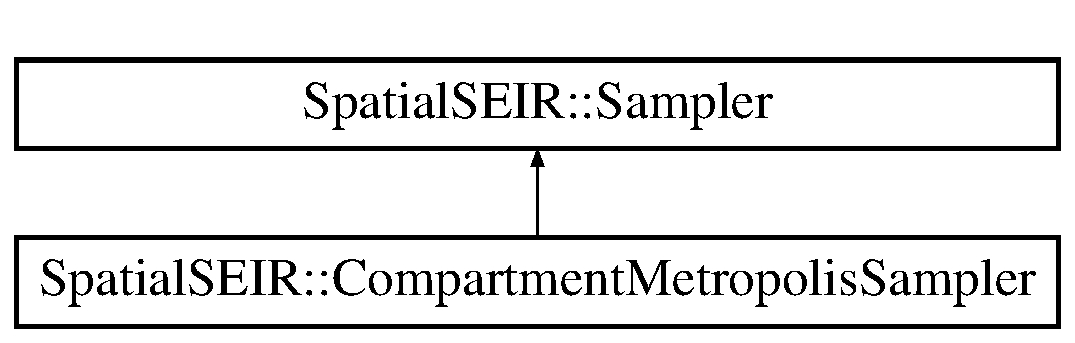
\includegraphics[height=2.000000cm]{classSpatialSEIR_1_1CompartmentMetropolisSampler}
\end{center}
\end{figure}
\subsection*{Public Member Functions}
\begin{DoxyCompactItemize}
\item 
\hyperlink{classSpatialSEIR_1_1CompartmentMetropolisSampler_af86755297ccbf562a108e653c8cb464d}{Compartment\-Metropolis\-Sampler} (\hyperlink{classSpatialSEIR_1_1ModelContext}{Model\-Context} $\ast$\hyperlink{classSpatialSEIR_1_1CompartmentMetropolisSampler_a17778f2c1b66d39a71a8fb6f5f648387}{context}, \hyperlink{classSpatialSEIR_1_1CompartmentFullConditional}{Compartment\-Full\-Conditional} $\ast$\hyperlink{classSpatialSEIR_1_1CompartmentMetropolisSampler_a917c4ed20e389f460e1cef15aeb51570}{compartment\-F\-C}, int $\ast$\hyperlink{classSpatialSEIR_1_1CompartmentMetropolisSampler_a82cb72e43365eddeec151023eca5af54}{compartment\-Data})
\item 
void \hyperlink{classSpatialSEIR_1_1CompartmentMetropolisSampler_a9d19f29ea0a8b86abb3e2082b469aed5}{draw\-Sample} ()
\item 
int \hyperlink{classSpatialSEIR_1_1CompartmentMetropolisSampler_a249b461e6f848c20f274bac7cae76e95}{get\-Sampler\-Type} ()
\item 
\hyperlink{classSpatialSEIR_1_1CompartmentMetropolisSampler_aadd072a410f46715097df75db53385be}{$\sim$\-Compartment\-Metropolis\-Sampler} ()
\end{DoxyCompactItemize}
\subsection*{Public Attributes}
\begin{DoxyCompactItemize}
\item 
\hyperlink{classSpatialSEIR_1_1ModelContext}{Model\-Context} $\ast$$\ast$ \hyperlink{classSpatialSEIR_1_1CompartmentMetropolisSampler_a17778f2c1b66d39a71a8fb6f5f648387}{context}
\item 
\hyperlink{classSpatialSEIR_1_1CompartmentFullConditional}{Compartment\-Full\-Conditional} $\ast$$\ast$ \hyperlink{classSpatialSEIR_1_1CompartmentMetropolisSampler_a917c4ed20e389f460e1cef15aeb51570}{compartment\-F\-C}
\item 
int $\ast$$\ast$ \hyperlink{classSpatialSEIR_1_1CompartmentMetropolisSampler_a82cb72e43365eddeec151023eca5af54}{compartment\-Data}
\end{DoxyCompactItemize}


\subsection{Detailed Description}
The \hyperlink{classSpatialSEIR_1_1CompartmentMetropolisSampler}{Compartment\-Metropolis\-Sampler} class is child of the \hyperlink{classSpatialSEIR_1_1Sampler}{Sampler} class which draws samples from the posterior distribution of the various transition compartments using a full compartment Metropolis proposal. 

\subsection{Constructor \& Destructor Documentation}
\hypertarget{classSpatialSEIR_1_1CompartmentMetropolisSampler_af86755297ccbf562a108e653c8cb464d}{\index{Spatial\-S\-E\-I\-R\-::\-Compartment\-Metropolis\-Sampler@{Spatial\-S\-E\-I\-R\-::\-Compartment\-Metropolis\-Sampler}!Compartment\-Metropolis\-Sampler@{Compartment\-Metropolis\-Sampler}}
\index{Compartment\-Metropolis\-Sampler@{Compartment\-Metropolis\-Sampler}!SpatialSEIR::CompartmentMetropolisSampler@{Spatial\-S\-E\-I\-R\-::\-Compartment\-Metropolis\-Sampler}}
\subsubsection[{Compartment\-Metropolis\-Sampler}]{\setlength{\rightskip}{0pt plus 5cm}Spatial\-S\-E\-I\-R\-::\-Compartment\-Metropolis\-Sampler\-::\-Compartment\-Metropolis\-Sampler (
\begin{DoxyParamCaption}
\item[{{\bf Model\-Context} $\ast$}]{context, }
\item[{{\bf Compartment\-Full\-Conditional} $\ast$}]{compartment\-F\-C, }
\item[{int $\ast$}]{compartment\-Data}
\end{DoxyParamCaption}
)}}\label{classSpatialSEIR_1_1CompartmentMetropolisSampler_af86755297ccbf562a108e653c8cb464d}
\hypertarget{classSpatialSEIR_1_1CompartmentMetropolisSampler_aadd072a410f46715097df75db53385be}{\index{Spatial\-S\-E\-I\-R\-::\-Compartment\-Metropolis\-Sampler@{Spatial\-S\-E\-I\-R\-::\-Compartment\-Metropolis\-Sampler}!$\sim$\-Compartment\-Metropolis\-Sampler@{$\sim$\-Compartment\-Metropolis\-Sampler}}
\index{$\sim$\-Compartment\-Metropolis\-Sampler@{$\sim$\-Compartment\-Metropolis\-Sampler}!SpatialSEIR::CompartmentMetropolisSampler@{Spatial\-S\-E\-I\-R\-::\-Compartment\-Metropolis\-Sampler}}
\subsubsection[{$\sim$\-Compartment\-Metropolis\-Sampler}]{\setlength{\rightskip}{0pt plus 5cm}Spatial\-S\-E\-I\-R\-::\-Compartment\-Metropolis\-Sampler\-::$\sim$\-Compartment\-Metropolis\-Sampler (
\begin{DoxyParamCaption}
{}
\end{DoxyParamCaption}
)}}\label{classSpatialSEIR_1_1CompartmentMetropolisSampler_aadd072a410f46715097df75db53385be}


\subsection{Member Function Documentation}
\hypertarget{classSpatialSEIR_1_1CompartmentMetropolisSampler_a9d19f29ea0a8b86abb3e2082b469aed5}{\index{Spatial\-S\-E\-I\-R\-::\-Compartment\-Metropolis\-Sampler@{Spatial\-S\-E\-I\-R\-::\-Compartment\-Metropolis\-Sampler}!draw\-Sample@{draw\-Sample}}
\index{draw\-Sample@{draw\-Sample}!SpatialSEIR::CompartmentMetropolisSampler@{Spatial\-S\-E\-I\-R\-::\-Compartment\-Metropolis\-Sampler}}
\subsubsection[{draw\-Sample}]{\setlength{\rightskip}{0pt plus 5cm}void Spatial\-S\-E\-I\-R\-::\-Compartment\-Metropolis\-Sampler\-::draw\-Sample (
\begin{DoxyParamCaption}
{}
\end{DoxyParamCaption}
)\hspace{0.3cm}{\ttfamily [virtual]}}}\label{classSpatialSEIR_1_1CompartmentMetropolisSampler_a9d19f29ea0a8b86abb3e2082b469aed5}


Implements \hyperlink{classSpatialSEIR_1_1Sampler_aa07a42b26cb62249c20c58e855a08657}{Spatial\-S\-E\-I\-R\-::\-Sampler}.

\hypertarget{classSpatialSEIR_1_1CompartmentMetropolisSampler_a249b461e6f848c20f274bac7cae76e95}{\index{Spatial\-S\-E\-I\-R\-::\-Compartment\-Metropolis\-Sampler@{Spatial\-S\-E\-I\-R\-::\-Compartment\-Metropolis\-Sampler}!get\-Sampler\-Type@{get\-Sampler\-Type}}
\index{get\-Sampler\-Type@{get\-Sampler\-Type}!SpatialSEIR::CompartmentMetropolisSampler@{Spatial\-S\-E\-I\-R\-::\-Compartment\-Metropolis\-Sampler}}
\subsubsection[{get\-Sampler\-Type}]{\setlength{\rightskip}{0pt plus 5cm}int Spatial\-S\-E\-I\-R\-::\-Compartment\-Metropolis\-Sampler\-::get\-Sampler\-Type (
\begin{DoxyParamCaption}
{}
\end{DoxyParamCaption}
)\hspace{0.3cm}{\ttfamily [virtual]}}}\label{classSpatialSEIR_1_1CompartmentMetropolisSampler_a249b461e6f848c20f274bac7cae76e95}


Implements \hyperlink{classSpatialSEIR_1_1Sampler_aaa79310ad809e6aeb25479849f322dda}{Spatial\-S\-E\-I\-R\-::\-Sampler}.



\subsection{Member Data Documentation}
\hypertarget{classSpatialSEIR_1_1CompartmentMetropolisSampler_a82cb72e43365eddeec151023eca5af54}{\index{Spatial\-S\-E\-I\-R\-::\-Compartment\-Metropolis\-Sampler@{Spatial\-S\-E\-I\-R\-::\-Compartment\-Metropolis\-Sampler}!compartment\-Data@{compartment\-Data}}
\index{compartment\-Data@{compartment\-Data}!SpatialSEIR::CompartmentMetropolisSampler@{Spatial\-S\-E\-I\-R\-::\-Compartment\-Metropolis\-Sampler}}
\subsubsection[{compartment\-Data}]{\setlength{\rightskip}{0pt plus 5cm}int$\ast$$\ast$ Spatial\-S\-E\-I\-R\-::\-Compartment\-Metropolis\-Sampler\-::compartment\-Data}}\label{classSpatialSEIR_1_1CompartmentMetropolisSampler_a82cb72e43365eddeec151023eca5af54}
\hypertarget{classSpatialSEIR_1_1CompartmentMetropolisSampler_a917c4ed20e389f460e1cef15aeb51570}{\index{Spatial\-S\-E\-I\-R\-::\-Compartment\-Metropolis\-Sampler@{Spatial\-S\-E\-I\-R\-::\-Compartment\-Metropolis\-Sampler}!compartment\-F\-C@{compartment\-F\-C}}
\index{compartment\-F\-C@{compartment\-F\-C}!SpatialSEIR::CompartmentMetropolisSampler@{Spatial\-S\-E\-I\-R\-::\-Compartment\-Metropolis\-Sampler}}
\subsubsection[{compartment\-F\-C}]{\setlength{\rightskip}{0pt plus 5cm}{\bf Compartment\-Full\-Conditional}$\ast$$\ast$ Spatial\-S\-E\-I\-R\-::\-Compartment\-Metropolis\-Sampler\-::compartment\-F\-C}}\label{classSpatialSEIR_1_1CompartmentMetropolisSampler_a917c4ed20e389f460e1cef15aeb51570}
\hypertarget{classSpatialSEIR_1_1CompartmentMetropolisSampler_a17778f2c1b66d39a71a8fb6f5f648387}{\index{Spatial\-S\-E\-I\-R\-::\-Compartment\-Metropolis\-Sampler@{Spatial\-S\-E\-I\-R\-::\-Compartment\-Metropolis\-Sampler}!context@{context}}
\index{context@{context}!SpatialSEIR::CompartmentMetropolisSampler@{Spatial\-S\-E\-I\-R\-::\-Compartment\-Metropolis\-Sampler}}
\subsubsection[{context}]{\setlength{\rightskip}{0pt plus 5cm}{\bf Model\-Context}$\ast$$\ast$ Spatial\-S\-E\-I\-R\-::\-Compartment\-Metropolis\-Sampler\-::context}}\label{classSpatialSEIR_1_1CompartmentMetropolisSampler_a17778f2c1b66d39a71a8fb6f5f648387}


The documentation for this class was generated from the following file\-:\begin{DoxyCompactItemize}
\item 
lib\-Spatial\-S\-E\-I\-R/include/\hyperlink{LSS__Samplers_8hpp}{L\-S\-S\-\_\-\-Samplers.\-hpp}\end{DoxyCompactItemize}

\hypertarget{classSpatialSEIR_1_1CompartmentMetropolisSampler__OCL}{\section{Spatial\-S\-E\-I\-R\-:\-:Compartment\-Metropolis\-Sampler\-\_\-\-O\-C\-L Class Reference}
\label{classSpatialSEIR_1_1CompartmentMetropolisSampler__OCL}\index{Spatial\-S\-E\-I\-R\-::\-Compartment\-Metropolis\-Sampler\-\_\-\-O\-C\-L@{Spatial\-S\-E\-I\-R\-::\-Compartment\-Metropolis\-Sampler\-\_\-\-O\-C\-L}}
}


{\ttfamily \#include $<$L\-S\-S\-\_\-\-Samplers.\-hpp$>$}

Inheritance diagram for Spatial\-S\-E\-I\-R\-:\-:Compartment\-Metropolis\-Sampler\-\_\-\-O\-C\-L\-:\begin{figure}[H]
\begin{center}
\leavevmode
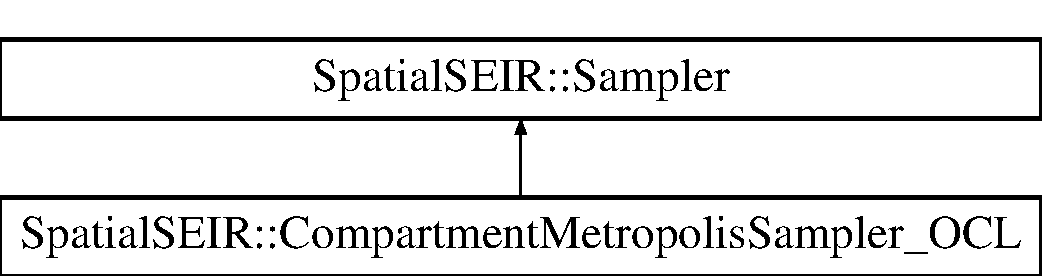
\includegraphics[height=2.000000cm]{classSpatialSEIR_1_1CompartmentMetropolisSampler__OCL}
\end{center}
\end{figure}
\subsection*{Public Member Functions}
\begin{DoxyCompactItemize}
\item 
\hyperlink{classSpatialSEIR_1_1CompartmentMetropolisSampler__OCL_a02fa309e6095b0450252d449fa71dc19}{Compartment\-Metropolis\-Sampler\-\_\-\-O\-C\-L} (\hyperlink{classSpatialSEIR_1_1ModelContext}{Model\-Context} $\ast$\hyperlink{classSpatialSEIR_1_1CompartmentMetropolisSampler__OCL_a231d67f96a0b9e2834b600804f1b06a1}{context}, \hyperlink{classSpatialSEIR_1_1CompartmentFullConditional}{Compartment\-Full\-Conditional} $\ast$\hyperlink{classSpatialSEIR_1_1CompartmentMetropolisSampler__OCL_a794de19e975d79673a8c7b9c952ce075}{compartment\-F\-C}, int $\ast$\hyperlink{classSpatialSEIR_1_1CompartmentMetropolisSampler__OCL_a4bcbbab42aac73ed628addf8d7a93526}{compartment\-Data})
\item 
void \hyperlink{classSpatialSEIR_1_1CompartmentMetropolisSampler__OCL_a7a0a9120eab5a44797f9255df6f89c2a}{draw\-Sample} ()
\item 
int \hyperlink{classSpatialSEIR_1_1CompartmentMetropolisSampler__OCL_a15b18cebae437f578fbf15aa8cfbdf94}{get\-Sampler\-Type} ()
\item 
\hyperlink{classSpatialSEIR_1_1CompartmentMetropolisSampler__OCL_ad3ca68f1d4d230fb3c9af13ee317832a}{$\sim$\-Compartment\-Metropolis\-Sampler\-\_\-\-O\-C\-L} ()
\end{DoxyCompactItemize}
\subsection*{Public Attributes}
\begin{DoxyCompactItemize}
\item 
\hyperlink{classSpatialSEIR_1_1ModelContext}{Model\-Context} $\ast$$\ast$ \hyperlink{classSpatialSEIR_1_1CompartmentMetropolisSampler__OCL_a231d67f96a0b9e2834b600804f1b06a1}{context}
\item 
\hyperlink{classSpatialSEIR_1_1CompartmentFullConditional}{Compartment\-Full\-Conditional} $\ast$$\ast$ \hyperlink{classSpatialSEIR_1_1CompartmentMetropolisSampler__OCL_a794de19e975d79673a8c7b9c952ce075}{compartment\-F\-C}
\item 
int $\ast$$\ast$ \hyperlink{classSpatialSEIR_1_1CompartmentMetropolisSampler__OCL_a4bcbbab42aac73ed628addf8d7a93526}{compartment\-Data}
\end{DoxyCompactItemize}


\subsection{Detailed Description}
The \hyperlink{classSpatialSEIR_1_1CompartmentMetropolisSampler__OCL}{Compartment\-Metropolis\-Sampler\-\_\-\-O\-C\-L} class is child of the \hyperlink{classSpatialSEIR_1_1Sampler}{Sampler} class which draws samples from the posterior distribution of the various transition compartments using a full compartment Metropolis proposal. This version of the Metropolis sampler uses the available Open\-C\-L features of libspatial\-S\-E\-I\-R. 

\subsection{Constructor \& Destructor Documentation}
\hypertarget{classSpatialSEIR_1_1CompartmentMetropolisSampler__OCL_a02fa309e6095b0450252d449fa71dc19}{\index{Spatial\-S\-E\-I\-R\-::\-Compartment\-Metropolis\-Sampler\-\_\-\-O\-C\-L@{Spatial\-S\-E\-I\-R\-::\-Compartment\-Metropolis\-Sampler\-\_\-\-O\-C\-L}!Compartment\-Metropolis\-Sampler\-\_\-\-O\-C\-L@{Compartment\-Metropolis\-Sampler\-\_\-\-O\-C\-L}}
\index{Compartment\-Metropolis\-Sampler\-\_\-\-O\-C\-L@{Compartment\-Metropolis\-Sampler\-\_\-\-O\-C\-L}!SpatialSEIR::CompartmentMetropolisSampler_OCL@{Spatial\-S\-E\-I\-R\-::\-Compartment\-Metropolis\-Sampler\-\_\-\-O\-C\-L}}
\subsubsection[{Compartment\-Metropolis\-Sampler\-\_\-\-O\-C\-L}]{\setlength{\rightskip}{0pt plus 5cm}Spatial\-S\-E\-I\-R\-::\-Compartment\-Metropolis\-Sampler\-\_\-\-O\-C\-L\-::\-Compartment\-Metropolis\-Sampler\-\_\-\-O\-C\-L (
\begin{DoxyParamCaption}
\item[{{\bf Model\-Context} $\ast$}]{context, }
\item[{{\bf Compartment\-Full\-Conditional} $\ast$}]{compartment\-F\-C, }
\item[{int $\ast$}]{compartment\-Data}
\end{DoxyParamCaption}
)}}\label{classSpatialSEIR_1_1CompartmentMetropolisSampler__OCL_a02fa309e6095b0450252d449fa71dc19}
\hypertarget{classSpatialSEIR_1_1CompartmentMetropolisSampler__OCL_ad3ca68f1d4d230fb3c9af13ee317832a}{\index{Spatial\-S\-E\-I\-R\-::\-Compartment\-Metropolis\-Sampler\-\_\-\-O\-C\-L@{Spatial\-S\-E\-I\-R\-::\-Compartment\-Metropolis\-Sampler\-\_\-\-O\-C\-L}!$\sim$\-Compartment\-Metropolis\-Sampler\-\_\-\-O\-C\-L@{$\sim$\-Compartment\-Metropolis\-Sampler\-\_\-\-O\-C\-L}}
\index{$\sim$\-Compartment\-Metropolis\-Sampler\-\_\-\-O\-C\-L@{$\sim$\-Compartment\-Metropolis\-Sampler\-\_\-\-O\-C\-L}!SpatialSEIR::CompartmentMetropolisSampler_OCL@{Spatial\-S\-E\-I\-R\-::\-Compartment\-Metropolis\-Sampler\-\_\-\-O\-C\-L}}
\subsubsection[{$\sim$\-Compartment\-Metropolis\-Sampler\-\_\-\-O\-C\-L}]{\setlength{\rightskip}{0pt plus 5cm}Spatial\-S\-E\-I\-R\-::\-Compartment\-Metropolis\-Sampler\-\_\-\-O\-C\-L\-::$\sim$\-Compartment\-Metropolis\-Sampler\-\_\-\-O\-C\-L (
\begin{DoxyParamCaption}
{}
\end{DoxyParamCaption}
)}}\label{classSpatialSEIR_1_1CompartmentMetropolisSampler__OCL_ad3ca68f1d4d230fb3c9af13ee317832a}


\subsection{Member Function Documentation}
\hypertarget{classSpatialSEIR_1_1CompartmentMetropolisSampler__OCL_a7a0a9120eab5a44797f9255df6f89c2a}{\index{Spatial\-S\-E\-I\-R\-::\-Compartment\-Metropolis\-Sampler\-\_\-\-O\-C\-L@{Spatial\-S\-E\-I\-R\-::\-Compartment\-Metropolis\-Sampler\-\_\-\-O\-C\-L}!draw\-Sample@{draw\-Sample}}
\index{draw\-Sample@{draw\-Sample}!SpatialSEIR::CompartmentMetropolisSampler_OCL@{Spatial\-S\-E\-I\-R\-::\-Compartment\-Metropolis\-Sampler\-\_\-\-O\-C\-L}}
\subsubsection[{draw\-Sample}]{\setlength{\rightskip}{0pt plus 5cm}void Spatial\-S\-E\-I\-R\-::\-Compartment\-Metropolis\-Sampler\-\_\-\-O\-C\-L\-::draw\-Sample (
\begin{DoxyParamCaption}
{}
\end{DoxyParamCaption}
)\hspace{0.3cm}{\ttfamily [virtual]}}}\label{classSpatialSEIR_1_1CompartmentMetropolisSampler__OCL_a7a0a9120eab5a44797f9255df6f89c2a}


Implements \hyperlink{classSpatialSEIR_1_1Sampler_aa07a42b26cb62249c20c58e855a08657}{Spatial\-S\-E\-I\-R\-::\-Sampler}.

\hypertarget{classSpatialSEIR_1_1CompartmentMetropolisSampler__OCL_a15b18cebae437f578fbf15aa8cfbdf94}{\index{Spatial\-S\-E\-I\-R\-::\-Compartment\-Metropolis\-Sampler\-\_\-\-O\-C\-L@{Spatial\-S\-E\-I\-R\-::\-Compartment\-Metropolis\-Sampler\-\_\-\-O\-C\-L}!get\-Sampler\-Type@{get\-Sampler\-Type}}
\index{get\-Sampler\-Type@{get\-Sampler\-Type}!SpatialSEIR::CompartmentMetropolisSampler_OCL@{Spatial\-S\-E\-I\-R\-::\-Compartment\-Metropolis\-Sampler\-\_\-\-O\-C\-L}}
\subsubsection[{get\-Sampler\-Type}]{\setlength{\rightskip}{0pt plus 5cm}int Spatial\-S\-E\-I\-R\-::\-Compartment\-Metropolis\-Sampler\-\_\-\-O\-C\-L\-::get\-Sampler\-Type (
\begin{DoxyParamCaption}
{}
\end{DoxyParamCaption}
)\hspace{0.3cm}{\ttfamily [virtual]}}}\label{classSpatialSEIR_1_1CompartmentMetropolisSampler__OCL_a15b18cebae437f578fbf15aa8cfbdf94}


Implements \hyperlink{classSpatialSEIR_1_1Sampler_aaa79310ad809e6aeb25479849f322dda}{Spatial\-S\-E\-I\-R\-::\-Sampler}.



\subsection{Member Data Documentation}
\hypertarget{classSpatialSEIR_1_1CompartmentMetropolisSampler__OCL_a4bcbbab42aac73ed628addf8d7a93526}{\index{Spatial\-S\-E\-I\-R\-::\-Compartment\-Metropolis\-Sampler\-\_\-\-O\-C\-L@{Spatial\-S\-E\-I\-R\-::\-Compartment\-Metropolis\-Sampler\-\_\-\-O\-C\-L}!compartment\-Data@{compartment\-Data}}
\index{compartment\-Data@{compartment\-Data}!SpatialSEIR::CompartmentMetropolisSampler_OCL@{Spatial\-S\-E\-I\-R\-::\-Compartment\-Metropolis\-Sampler\-\_\-\-O\-C\-L}}
\subsubsection[{compartment\-Data}]{\setlength{\rightskip}{0pt plus 5cm}int$\ast$$\ast$ Spatial\-S\-E\-I\-R\-::\-Compartment\-Metropolis\-Sampler\-\_\-\-O\-C\-L\-::compartment\-Data}}\label{classSpatialSEIR_1_1CompartmentMetropolisSampler__OCL_a4bcbbab42aac73ed628addf8d7a93526}
\hypertarget{classSpatialSEIR_1_1CompartmentMetropolisSampler__OCL_a794de19e975d79673a8c7b9c952ce075}{\index{Spatial\-S\-E\-I\-R\-::\-Compartment\-Metropolis\-Sampler\-\_\-\-O\-C\-L@{Spatial\-S\-E\-I\-R\-::\-Compartment\-Metropolis\-Sampler\-\_\-\-O\-C\-L}!compartment\-F\-C@{compartment\-F\-C}}
\index{compartment\-F\-C@{compartment\-F\-C}!SpatialSEIR::CompartmentMetropolisSampler_OCL@{Spatial\-S\-E\-I\-R\-::\-Compartment\-Metropolis\-Sampler\-\_\-\-O\-C\-L}}
\subsubsection[{compartment\-F\-C}]{\setlength{\rightskip}{0pt plus 5cm}{\bf Compartment\-Full\-Conditional}$\ast$$\ast$ Spatial\-S\-E\-I\-R\-::\-Compartment\-Metropolis\-Sampler\-\_\-\-O\-C\-L\-::compartment\-F\-C}}\label{classSpatialSEIR_1_1CompartmentMetropolisSampler__OCL_a794de19e975d79673a8c7b9c952ce075}
\hypertarget{classSpatialSEIR_1_1CompartmentMetropolisSampler__OCL_a231d67f96a0b9e2834b600804f1b06a1}{\index{Spatial\-S\-E\-I\-R\-::\-Compartment\-Metropolis\-Sampler\-\_\-\-O\-C\-L@{Spatial\-S\-E\-I\-R\-::\-Compartment\-Metropolis\-Sampler\-\_\-\-O\-C\-L}!context@{context}}
\index{context@{context}!SpatialSEIR::CompartmentMetropolisSampler_OCL@{Spatial\-S\-E\-I\-R\-::\-Compartment\-Metropolis\-Sampler\-\_\-\-O\-C\-L}}
\subsubsection[{context}]{\setlength{\rightskip}{0pt plus 5cm}{\bf Model\-Context}$\ast$$\ast$ Spatial\-S\-E\-I\-R\-::\-Compartment\-Metropolis\-Sampler\-\_\-\-O\-C\-L\-::context}}\label{classSpatialSEIR_1_1CompartmentMetropolisSampler__OCL_a231d67f96a0b9e2834b600804f1b06a1}


The documentation for this class was generated from the following file\-:\begin{DoxyCompactItemize}
\item 
lib\-Spatial\-S\-E\-I\-R/include/\hyperlink{LSS__Samplers_8hpp}{L\-S\-S\-\_\-\-Samplers.\-hpp}\end{DoxyCompactItemize}

\hypertarget{structSpatialSEIR_1_1covariateArgs}{\section{Spatial\-S\-E\-I\-R\-:\-:covariate\-Args Struct Reference}
\label{structSpatialSEIR_1_1covariateArgs}\index{Spatial\-S\-E\-I\-R\-::covariate\-Args@{Spatial\-S\-E\-I\-R\-::covariate\-Args}}
}


{\ttfamily \#include $<$Covariate\-Matrix.\-hpp$>$}

\subsection*{Public Attributes}
\begin{DoxyCompactItemize}
\item 
double $\ast$ \hyperlink{structSpatialSEIR_1_1covariateArgs_a3e246842542e2b74da77f0f666d22dd1}{in\-Data\-\_\-x}
\item 
double $\ast$ \hyperlink{structSpatialSEIR_1_1covariateArgs_a43af9cbaf391c6143054ef57a809f6d8}{in\-Data\-\_\-z}
\item 
int $\ast$ \hyperlink{structSpatialSEIR_1_1covariateArgs_af1c371b03a94d277a43d9f5aecc117aa}{in\-Row\-\_\-x}
\item 
int $\ast$ \hyperlink{structSpatialSEIR_1_1covariateArgs_ab62fd8861e67e0911f1af78a0d77572e}{in\-Col\-\_\-x}
\item 
int $\ast$ \hyperlink{structSpatialSEIR_1_1covariateArgs_a669bcd8ad82576664761bb25bfaba53e}{in\-Row\-\_\-z}
\item 
int $\ast$ \hyperlink{structSpatialSEIR_1_1covariateArgs_a15b3c909a5218f2035bb03e4f21a5a95}{in\-Col\-\_\-z}
\end{DoxyCompactItemize}


\subsection{Member Data Documentation}
\hypertarget{structSpatialSEIR_1_1covariateArgs_ab62fd8861e67e0911f1af78a0d77572e}{\index{Spatial\-S\-E\-I\-R\-::covariate\-Args@{Spatial\-S\-E\-I\-R\-::covariate\-Args}!in\-Col\-\_\-x@{in\-Col\-\_\-x}}
\index{in\-Col\-\_\-x@{in\-Col\-\_\-x}!SpatialSEIR::covariateArgs@{Spatial\-S\-E\-I\-R\-::covariate\-Args}}
\subsubsection[{in\-Col\-\_\-x}]{\setlength{\rightskip}{0pt plus 5cm}int$\ast$ Spatial\-S\-E\-I\-R\-::covariate\-Args\-::in\-Col\-\_\-x}}\label{structSpatialSEIR_1_1covariateArgs_ab62fd8861e67e0911f1af78a0d77572e}
\hypertarget{structSpatialSEIR_1_1covariateArgs_a15b3c909a5218f2035bb03e4f21a5a95}{\index{Spatial\-S\-E\-I\-R\-::covariate\-Args@{Spatial\-S\-E\-I\-R\-::covariate\-Args}!in\-Col\-\_\-z@{in\-Col\-\_\-z}}
\index{in\-Col\-\_\-z@{in\-Col\-\_\-z}!SpatialSEIR::covariateArgs@{Spatial\-S\-E\-I\-R\-::covariate\-Args}}
\subsubsection[{in\-Col\-\_\-z}]{\setlength{\rightskip}{0pt plus 5cm}int$\ast$ Spatial\-S\-E\-I\-R\-::covariate\-Args\-::in\-Col\-\_\-z}}\label{structSpatialSEIR_1_1covariateArgs_a15b3c909a5218f2035bb03e4f21a5a95}
\hypertarget{structSpatialSEIR_1_1covariateArgs_a3e246842542e2b74da77f0f666d22dd1}{\index{Spatial\-S\-E\-I\-R\-::covariate\-Args@{Spatial\-S\-E\-I\-R\-::covariate\-Args}!in\-Data\-\_\-x@{in\-Data\-\_\-x}}
\index{in\-Data\-\_\-x@{in\-Data\-\_\-x}!SpatialSEIR::covariateArgs@{Spatial\-S\-E\-I\-R\-::covariate\-Args}}
\subsubsection[{in\-Data\-\_\-x}]{\setlength{\rightskip}{0pt plus 5cm}double$\ast$ Spatial\-S\-E\-I\-R\-::covariate\-Args\-::in\-Data\-\_\-x}}\label{structSpatialSEIR_1_1covariateArgs_a3e246842542e2b74da77f0f666d22dd1}
\hypertarget{structSpatialSEIR_1_1covariateArgs_a43af9cbaf391c6143054ef57a809f6d8}{\index{Spatial\-S\-E\-I\-R\-::covariate\-Args@{Spatial\-S\-E\-I\-R\-::covariate\-Args}!in\-Data\-\_\-z@{in\-Data\-\_\-z}}
\index{in\-Data\-\_\-z@{in\-Data\-\_\-z}!SpatialSEIR::covariateArgs@{Spatial\-S\-E\-I\-R\-::covariate\-Args}}
\subsubsection[{in\-Data\-\_\-z}]{\setlength{\rightskip}{0pt plus 5cm}double$\ast$ Spatial\-S\-E\-I\-R\-::covariate\-Args\-::in\-Data\-\_\-z}}\label{structSpatialSEIR_1_1covariateArgs_a43af9cbaf391c6143054ef57a809f6d8}
\hypertarget{structSpatialSEIR_1_1covariateArgs_af1c371b03a94d277a43d9f5aecc117aa}{\index{Spatial\-S\-E\-I\-R\-::covariate\-Args@{Spatial\-S\-E\-I\-R\-::covariate\-Args}!in\-Row\-\_\-x@{in\-Row\-\_\-x}}
\index{in\-Row\-\_\-x@{in\-Row\-\_\-x}!SpatialSEIR::covariateArgs@{Spatial\-S\-E\-I\-R\-::covariate\-Args}}
\subsubsection[{in\-Row\-\_\-x}]{\setlength{\rightskip}{0pt plus 5cm}int$\ast$ Spatial\-S\-E\-I\-R\-::covariate\-Args\-::in\-Row\-\_\-x}}\label{structSpatialSEIR_1_1covariateArgs_af1c371b03a94d277a43d9f5aecc117aa}
\hypertarget{structSpatialSEIR_1_1covariateArgs_a669bcd8ad82576664761bb25bfaba53e}{\index{Spatial\-S\-E\-I\-R\-::covariate\-Args@{Spatial\-S\-E\-I\-R\-::covariate\-Args}!in\-Row\-\_\-z@{in\-Row\-\_\-z}}
\index{in\-Row\-\_\-z@{in\-Row\-\_\-z}!SpatialSEIR::covariateArgs@{Spatial\-S\-E\-I\-R\-::covariate\-Args}}
\subsubsection[{in\-Row\-\_\-z}]{\setlength{\rightskip}{0pt plus 5cm}int$\ast$ Spatial\-S\-E\-I\-R\-::covariate\-Args\-::in\-Row\-\_\-z}}\label{structSpatialSEIR_1_1covariateArgs_a669bcd8ad82576664761bb25bfaba53e}


The documentation for this struct was generated from the following file\-:\begin{DoxyCompactItemize}
\item 
lib\-Spatial\-S\-E\-I\-R/include/\-Data\-Structures/\hyperlink{CovariateMatrix_8hpp}{Covariate\-Matrix.\-hpp}\end{DoxyCompactItemize}

\hypertarget{classSpatialSEIR_1_1CovariateMatrix}{\section{Spatial\-S\-E\-I\-R\-:\-:Covariate\-Matrix Class Reference}
\label{classSpatialSEIR_1_1CovariateMatrix}\index{Spatial\-S\-E\-I\-R\-::\-Covariate\-Matrix@{Spatial\-S\-E\-I\-R\-::\-Covariate\-Matrix}}
}


{\ttfamily \#include $<$Covariate\-Matrix.\-hpp$>$}

\subsection*{Public Member Functions}
\begin{DoxyCompactItemize}
\item 
int \hyperlink{classSpatialSEIR_1_1CovariateMatrix_a6d01e75564364a8f3356c3cee02bf43d}{gen\-From\-Data\-Stream} (double $\ast$indata\-\_\-x, double $\ast$indata\-\_\-z, int $\ast$inrow\-\_\-x, int $\ast$incol\-\_\-x, int $\ast$inrow\-\_\-z, int $\ast$incol\-\_\-z)
\item 
int \hyperlink{classSpatialSEIR_1_1CovariateMatrix_a385a3e444e0e92993db6d50440a1c254}{calculate\-\_\-fixed\-\_\-eta\-\_\-\-C\-P\-U} (double $\ast$eta, double $\ast$beta)
\item 
int \hyperlink{classSpatialSEIR_1_1CovariateMatrix_ad99c3e064edae9c73aa30b5f68628c15}{calculate\-\_\-eta\-\_\-\-C\-P\-U} (double $\ast$eta, double $\ast$beta)
\item 
int \hyperlink{classSpatialSEIR_1_1CovariateMatrix_af9eed26337877e698c4077c2548aedd3}{calculate\-\_\-eta\-\_\-\-O\-C\-L} (double $\ast$eta, double $\ast$beta)
\item 
void \hyperlink{classSpatialSEIR_1_1CovariateMatrix_a094a15fd40f4a6920c3df909b11761f6}{build\-Decorrelation\-Projection\-Matrix} ()
\item 
\hyperlink{classSpatialSEIR_1_1CovariateMatrix_a249c8173d32d887ee3beb492e8f9dad1}{$\sim$\-Covariate\-Matrix} ()
\end{DoxyCompactItemize}
\subsection*{Public Attributes}
\begin{DoxyCompactItemize}
\item 
double $\ast$ \hyperlink{classSpatialSEIR_1_1CovariateMatrix_a1db364bb68f755ff8fc15844ae429716}{X}
\item 
double $\ast$ \hyperlink{classSpatialSEIR_1_1CovariateMatrix_a148a63e712e2a3fabc928615e24acd78}{Z}
\item 
double $\ast$ \hyperlink{classSpatialSEIR_1_1CovariateMatrix_abdf2ed4c599a62b93e856a0bcbbcef2f}{decorrelation\-Projection\-Matrix}
\item 
double $\ast$ \hyperlink{classSpatialSEIR_1_1CovariateMatrix_aea38ad4cbebd1c82842cf3c389c93856}{offset}
\item 
int $\ast$ \hyperlink{classSpatialSEIR_1_1CovariateMatrix_a85ba097a370463b0b96e1ab76791f681}{offset\-Length}
\item 
std\-::vector$<$ std\-::string $>$ $\ast$ \hyperlink{classSpatialSEIR_1_1CovariateMatrix_ad537dcde3bcf55230b30e2c68d9497f6}{varnames}
\item 
int $\ast$ \hyperlink{classSpatialSEIR_1_1CovariateMatrix_afd333a01394a5aea9ccd3cb34f781a59}{nrow\-\_\-x}
\item 
int $\ast$ \hyperlink{classSpatialSEIR_1_1CovariateMatrix_a84e9369443cf51230067605b13a36702}{ncol\-\_\-x}
\item 
int $\ast$ \hyperlink{classSpatialSEIR_1_1CovariateMatrix_a01bcdc77f58b3f98fea4f3fb20edbeae}{nrow\-\_\-z}
\item 
int $\ast$ \hyperlink{classSpatialSEIR_1_1CovariateMatrix_ac4e692ef3c7fe38cb0c383c561f4991e}{ncol\-\_\-z}
\end{DoxyCompactItemize}


\subsection{Constructor \& Destructor Documentation}
\hypertarget{classSpatialSEIR_1_1CovariateMatrix_a249c8173d32d887ee3beb492e8f9dad1}{\index{Spatial\-S\-E\-I\-R\-::\-Covariate\-Matrix@{Spatial\-S\-E\-I\-R\-::\-Covariate\-Matrix}!$\sim$\-Covariate\-Matrix@{$\sim$\-Covariate\-Matrix}}
\index{$\sim$\-Covariate\-Matrix@{$\sim$\-Covariate\-Matrix}!SpatialSEIR::CovariateMatrix@{Spatial\-S\-E\-I\-R\-::\-Covariate\-Matrix}}
\subsubsection[{$\sim$\-Covariate\-Matrix}]{\setlength{\rightskip}{0pt plus 5cm}Spatial\-S\-E\-I\-R\-::\-Covariate\-Matrix\-::$\sim$\-Covariate\-Matrix (
\begin{DoxyParamCaption}
{}
\end{DoxyParamCaption}
)}}\label{classSpatialSEIR_1_1CovariateMatrix_a249c8173d32d887ee3beb492e8f9dad1}


\subsection{Member Function Documentation}
\hypertarget{classSpatialSEIR_1_1CovariateMatrix_a094a15fd40f4a6920c3df909b11761f6}{\index{Spatial\-S\-E\-I\-R\-::\-Covariate\-Matrix@{Spatial\-S\-E\-I\-R\-::\-Covariate\-Matrix}!build\-Decorrelation\-Projection\-Matrix@{build\-Decorrelation\-Projection\-Matrix}}
\index{build\-Decorrelation\-Projection\-Matrix@{build\-Decorrelation\-Projection\-Matrix}!SpatialSEIR::CovariateMatrix@{Spatial\-S\-E\-I\-R\-::\-Covariate\-Matrix}}
\subsubsection[{build\-Decorrelation\-Projection\-Matrix}]{\setlength{\rightskip}{0pt plus 5cm}void Spatial\-S\-E\-I\-R\-::\-Covariate\-Matrix\-::build\-Decorrelation\-Projection\-Matrix (
\begin{DoxyParamCaption}
{}
\end{DoxyParamCaption}
)}}\label{classSpatialSEIR_1_1CovariateMatrix_a094a15fd40f4a6920c3df909b11761f6}
\hypertarget{classSpatialSEIR_1_1CovariateMatrix_ad99c3e064edae9c73aa30b5f68628c15}{\index{Spatial\-S\-E\-I\-R\-::\-Covariate\-Matrix@{Spatial\-S\-E\-I\-R\-::\-Covariate\-Matrix}!calculate\-\_\-eta\-\_\-\-C\-P\-U@{calculate\-\_\-eta\-\_\-\-C\-P\-U}}
\index{calculate\-\_\-eta\-\_\-\-C\-P\-U@{calculate\-\_\-eta\-\_\-\-C\-P\-U}!SpatialSEIR::CovariateMatrix@{Spatial\-S\-E\-I\-R\-::\-Covariate\-Matrix}}
\subsubsection[{calculate\-\_\-eta\-\_\-\-C\-P\-U}]{\setlength{\rightskip}{0pt plus 5cm}int Spatial\-S\-E\-I\-R\-::\-Covariate\-Matrix\-::calculate\-\_\-eta\-\_\-\-C\-P\-U (
\begin{DoxyParamCaption}
\item[{double $\ast$}]{eta, }
\item[{double $\ast$}]{beta}
\end{DoxyParamCaption}
)}}\label{classSpatialSEIR_1_1CovariateMatrix_ad99c3e064edae9c73aa30b5f68628c15}
\hypertarget{classSpatialSEIR_1_1CovariateMatrix_af9eed26337877e698c4077c2548aedd3}{\index{Spatial\-S\-E\-I\-R\-::\-Covariate\-Matrix@{Spatial\-S\-E\-I\-R\-::\-Covariate\-Matrix}!calculate\-\_\-eta\-\_\-\-O\-C\-L@{calculate\-\_\-eta\-\_\-\-O\-C\-L}}
\index{calculate\-\_\-eta\-\_\-\-O\-C\-L@{calculate\-\_\-eta\-\_\-\-O\-C\-L}!SpatialSEIR::CovariateMatrix@{Spatial\-S\-E\-I\-R\-::\-Covariate\-Matrix}}
\subsubsection[{calculate\-\_\-eta\-\_\-\-O\-C\-L}]{\setlength{\rightskip}{0pt plus 5cm}int Spatial\-S\-E\-I\-R\-::\-Covariate\-Matrix\-::calculate\-\_\-eta\-\_\-\-O\-C\-L (
\begin{DoxyParamCaption}
\item[{double $\ast$}]{eta, }
\item[{double $\ast$}]{beta}
\end{DoxyParamCaption}
)}}\label{classSpatialSEIR_1_1CovariateMatrix_af9eed26337877e698c4077c2548aedd3}
\hypertarget{classSpatialSEIR_1_1CovariateMatrix_a385a3e444e0e92993db6d50440a1c254}{\index{Spatial\-S\-E\-I\-R\-::\-Covariate\-Matrix@{Spatial\-S\-E\-I\-R\-::\-Covariate\-Matrix}!calculate\-\_\-fixed\-\_\-eta\-\_\-\-C\-P\-U@{calculate\-\_\-fixed\-\_\-eta\-\_\-\-C\-P\-U}}
\index{calculate\-\_\-fixed\-\_\-eta\-\_\-\-C\-P\-U@{calculate\-\_\-fixed\-\_\-eta\-\_\-\-C\-P\-U}!SpatialSEIR::CovariateMatrix@{Spatial\-S\-E\-I\-R\-::\-Covariate\-Matrix}}
\subsubsection[{calculate\-\_\-fixed\-\_\-eta\-\_\-\-C\-P\-U}]{\setlength{\rightskip}{0pt plus 5cm}int Spatial\-S\-E\-I\-R\-::\-Covariate\-Matrix\-::calculate\-\_\-fixed\-\_\-eta\-\_\-\-C\-P\-U (
\begin{DoxyParamCaption}
\item[{double $\ast$}]{eta, }
\item[{double $\ast$}]{beta}
\end{DoxyParamCaption}
)}}\label{classSpatialSEIR_1_1CovariateMatrix_a385a3e444e0e92993db6d50440a1c254}
\hypertarget{classSpatialSEIR_1_1CovariateMatrix_a6d01e75564364a8f3356c3cee02bf43d}{\index{Spatial\-S\-E\-I\-R\-::\-Covariate\-Matrix@{Spatial\-S\-E\-I\-R\-::\-Covariate\-Matrix}!gen\-From\-Data\-Stream@{gen\-From\-Data\-Stream}}
\index{gen\-From\-Data\-Stream@{gen\-From\-Data\-Stream}!SpatialSEIR::CovariateMatrix@{Spatial\-S\-E\-I\-R\-::\-Covariate\-Matrix}}
\subsubsection[{gen\-From\-Data\-Stream}]{\setlength{\rightskip}{0pt plus 5cm}int Spatial\-S\-E\-I\-R\-::\-Covariate\-Matrix\-::gen\-From\-Data\-Stream (
\begin{DoxyParamCaption}
\item[{double $\ast$}]{indata\-\_\-x, }
\item[{double $\ast$}]{indata\-\_\-z, }
\item[{int $\ast$}]{inrow\-\_\-x, }
\item[{int $\ast$}]{incol\-\_\-x, }
\item[{int $\ast$}]{inrow\-\_\-z, }
\item[{int $\ast$}]{incol\-\_\-z}
\end{DoxyParamCaption}
)}}\label{classSpatialSEIR_1_1CovariateMatrix_a6d01e75564364a8f3356c3cee02bf43d}


\subsection{Member Data Documentation}
\hypertarget{classSpatialSEIR_1_1CovariateMatrix_abdf2ed4c599a62b93e856a0bcbbcef2f}{\index{Spatial\-S\-E\-I\-R\-::\-Covariate\-Matrix@{Spatial\-S\-E\-I\-R\-::\-Covariate\-Matrix}!decorrelation\-Projection\-Matrix@{decorrelation\-Projection\-Matrix}}
\index{decorrelation\-Projection\-Matrix@{decorrelation\-Projection\-Matrix}!SpatialSEIR::CovariateMatrix@{Spatial\-S\-E\-I\-R\-::\-Covariate\-Matrix}}
\subsubsection[{decorrelation\-Projection\-Matrix}]{\setlength{\rightskip}{0pt plus 5cm}double$\ast$ Spatial\-S\-E\-I\-R\-::\-Covariate\-Matrix\-::decorrelation\-Projection\-Matrix}}\label{classSpatialSEIR_1_1CovariateMatrix_abdf2ed4c599a62b93e856a0bcbbcef2f}
\hypertarget{classSpatialSEIR_1_1CovariateMatrix_a84e9369443cf51230067605b13a36702}{\index{Spatial\-S\-E\-I\-R\-::\-Covariate\-Matrix@{Spatial\-S\-E\-I\-R\-::\-Covariate\-Matrix}!ncol\-\_\-x@{ncol\-\_\-x}}
\index{ncol\-\_\-x@{ncol\-\_\-x}!SpatialSEIR::CovariateMatrix@{Spatial\-S\-E\-I\-R\-::\-Covariate\-Matrix}}
\subsubsection[{ncol\-\_\-x}]{\setlength{\rightskip}{0pt plus 5cm}int$\ast$ Spatial\-S\-E\-I\-R\-::\-Covariate\-Matrix\-::ncol\-\_\-x}}\label{classSpatialSEIR_1_1CovariateMatrix_a84e9369443cf51230067605b13a36702}
\hypertarget{classSpatialSEIR_1_1CovariateMatrix_ac4e692ef3c7fe38cb0c383c561f4991e}{\index{Spatial\-S\-E\-I\-R\-::\-Covariate\-Matrix@{Spatial\-S\-E\-I\-R\-::\-Covariate\-Matrix}!ncol\-\_\-z@{ncol\-\_\-z}}
\index{ncol\-\_\-z@{ncol\-\_\-z}!SpatialSEIR::CovariateMatrix@{Spatial\-S\-E\-I\-R\-::\-Covariate\-Matrix}}
\subsubsection[{ncol\-\_\-z}]{\setlength{\rightskip}{0pt plus 5cm}int$\ast$ Spatial\-S\-E\-I\-R\-::\-Covariate\-Matrix\-::ncol\-\_\-z}}\label{classSpatialSEIR_1_1CovariateMatrix_ac4e692ef3c7fe38cb0c383c561f4991e}
\hypertarget{classSpatialSEIR_1_1CovariateMatrix_afd333a01394a5aea9ccd3cb34f781a59}{\index{Spatial\-S\-E\-I\-R\-::\-Covariate\-Matrix@{Spatial\-S\-E\-I\-R\-::\-Covariate\-Matrix}!nrow\-\_\-x@{nrow\-\_\-x}}
\index{nrow\-\_\-x@{nrow\-\_\-x}!SpatialSEIR::CovariateMatrix@{Spatial\-S\-E\-I\-R\-::\-Covariate\-Matrix}}
\subsubsection[{nrow\-\_\-x}]{\setlength{\rightskip}{0pt plus 5cm}int$\ast$ Spatial\-S\-E\-I\-R\-::\-Covariate\-Matrix\-::nrow\-\_\-x}}\label{classSpatialSEIR_1_1CovariateMatrix_afd333a01394a5aea9ccd3cb34f781a59}
\hypertarget{classSpatialSEIR_1_1CovariateMatrix_a01bcdc77f58b3f98fea4f3fb20edbeae}{\index{Spatial\-S\-E\-I\-R\-::\-Covariate\-Matrix@{Spatial\-S\-E\-I\-R\-::\-Covariate\-Matrix}!nrow\-\_\-z@{nrow\-\_\-z}}
\index{nrow\-\_\-z@{nrow\-\_\-z}!SpatialSEIR::CovariateMatrix@{Spatial\-S\-E\-I\-R\-::\-Covariate\-Matrix}}
\subsubsection[{nrow\-\_\-z}]{\setlength{\rightskip}{0pt plus 5cm}int$\ast$ Spatial\-S\-E\-I\-R\-::\-Covariate\-Matrix\-::nrow\-\_\-z}}\label{classSpatialSEIR_1_1CovariateMatrix_a01bcdc77f58b3f98fea4f3fb20edbeae}
\hypertarget{classSpatialSEIR_1_1CovariateMatrix_aea38ad4cbebd1c82842cf3c389c93856}{\index{Spatial\-S\-E\-I\-R\-::\-Covariate\-Matrix@{Spatial\-S\-E\-I\-R\-::\-Covariate\-Matrix}!offset@{offset}}
\index{offset@{offset}!SpatialSEIR::CovariateMatrix@{Spatial\-S\-E\-I\-R\-::\-Covariate\-Matrix}}
\subsubsection[{offset}]{\setlength{\rightskip}{0pt plus 5cm}double$\ast$ Spatial\-S\-E\-I\-R\-::\-Covariate\-Matrix\-::offset}}\label{classSpatialSEIR_1_1CovariateMatrix_aea38ad4cbebd1c82842cf3c389c93856}
\hypertarget{classSpatialSEIR_1_1CovariateMatrix_a85ba097a370463b0b96e1ab76791f681}{\index{Spatial\-S\-E\-I\-R\-::\-Covariate\-Matrix@{Spatial\-S\-E\-I\-R\-::\-Covariate\-Matrix}!offset\-Length@{offset\-Length}}
\index{offset\-Length@{offset\-Length}!SpatialSEIR::CovariateMatrix@{Spatial\-S\-E\-I\-R\-::\-Covariate\-Matrix}}
\subsubsection[{offset\-Length}]{\setlength{\rightskip}{0pt plus 5cm}int$\ast$ Spatial\-S\-E\-I\-R\-::\-Covariate\-Matrix\-::offset\-Length}}\label{classSpatialSEIR_1_1CovariateMatrix_a85ba097a370463b0b96e1ab76791f681}
\hypertarget{classSpatialSEIR_1_1CovariateMatrix_ad537dcde3bcf55230b30e2c68d9497f6}{\index{Spatial\-S\-E\-I\-R\-::\-Covariate\-Matrix@{Spatial\-S\-E\-I\-R\-::\-Covariate\-Matrix}!varnames@{varnames}}
\index{varnames@{varnames}!SpatialSEIR::CovariateMatrix@{Spatial\-S\-E\-I\-R\-::\-Covariate\-Matrix}}
\subsubsection[{varnames}]{\setlength{\rightskip}{0pt plus 5cm}std\-::vector$<$std\-::string$>$$\ast$ Spatial\-S\-E\-I\-R\-::\-Covariate\-Matrix\-::varnames}}\label{classSpatialSEIR_1_1CovariateMatrix_ad537dcde3bcf55230b30e2c68d9497f6}
\hypertarget{classSpatialSEIR_1_1CovariateMatrix_a1db364bb68f755ff8fc15844ae429716}{\index{Spatial\-S\-E\-I\-R\-::\-Covariate\-Matrix@{Spatial\-S\-E\-I\-R\-::\-Covariate\-Matrix}!X@{X}}
\index{X@{X}!SpatialSEIR::CovariateMatrix@{Spatial\-S\-E\-I\-R\-::\-Covariate\-Matrix}}
\subsubsection[{X}]{\setlength{\rightskip}{0pt plus 5cm}double$\ast$ Spatial\-S\-E\-I\-R\-::\-Covariate\-Matrix\-::\-X}}\label{classSpatialSEIR_1_1CovariateMatrix_a1db364bb68f755ff8fc15844ae429716}
\hypertarget{classSpatialSEIR_1_1CovariateMatrix_a148a63e712e2a3fabc928615e24acd78}{\index{Spatial\-S\-E\-I\-R\-::\-Covariate\-Matrix@{Spatial\-S\-E\-I\-R\-::\-Covariate\-Matrix}!Z@{Z}}
\index{Z@{Z}!SpatialSEIR::CovariateMatrix@{Spatial\-S\-E\-I\-R\-::\-Covariate\-Matrix}}
\subsubsection[{Z}]{\setlength{\rightskip}{0pt plus 5cm}double$\ast$ Spatial\-S\-E\-I\-R\-::\-Covariate\-Matrix\-::\-Z}}\label{classSpatialSEIR_1_1CovariateMatrix_a148a63e712e2a3fabc928615e24acd78}


The documentation for this class was generated from the following files\-:\begin{DoxyCompactItemize}
\item 
lib\-Spatial\-S\-E\-I\-R/include/\-Data\-Structures/\hyperlink{CovariateMatrix_8hpp}{Covariate\-Matrix.\-hpp}\item 
lib\-Spatial\-S\-E\-I\-R/src/\hyperlink{CovariateMatrix_8cpp}{Covariate\-Matrix.\-cpp}\end{DoxyCompactItemize}

\hypertarget{structSpatialSEIR_1_1distanceArgs}{\section{Spatial\-S\-E\-I\-R\-:\-:distance\-Args Struct Reference}
\label{structSpatialSEIR_1_1distanceArgs}\index{Spatial\-S\-E\-I\-R\-::distance\-Args@{Spatial\-S\-E\-I\-R\-::distance\-Args}}
}


{\ttfamily \#include $<$Distance\-Matrix.\-hpp$>$}

\subsection*{Public Attributes}
\begin{DoxyCompactItemize}
\item 
std\-::vector$<$ double $\ast$ $>$ \hyperlink{structSpatialSEIR_1_1distanceArgs_a7f9cbfeb6d9812f3328a0de341a0488f}{in\-Data}
\item 
int $\ast$ \hyperlink{structSpatialSEIR_1_1distanceArgs_a9ec648afe9d6177599f9fe68f05df837}{dim}
\end{DoxyCompactItemize}


\subsection{Member Data Documentation}
\hypertarget{structSpatialSEIR_1_1distanceArgs_a9ec648afe9d6177599f9fe68f05df837}{\index{Spatial\-S\-E\-I\-R\-::distance\-Args@{Spatial\-S\-E\-I\-R\-::distance\-Args}!dim@{dim}}
\index{dim@{dim}!SpatialSEIR::distanceArgs@{Spatial\-S\-E\-I\-R\-::distance\-Args}}
\subsubsection[{dim}]{\setlength{\rightskip}{0pt plus 5cm}int$\ast$ Spatial\-S\-E\-I\-R\-::distance\-Args\-::dim}}\label{structSpatialSEIR_1_1distanceArgs_a9ec648afe9d6177599f9fe68f05df837}
\hypertarget{structSpatialSEIR_1_1distanceArgs_a7f9cbfeb6d9812f3328a0de341a0488f}{\index{Spatial\-S\-E\-I\-R\-::distance\-Args@{Spatial\-S\-E\-I\-R\-::distance\-Args}!in\-Data@{in\-Data}}
\index{in\-Data@{in\-Data}!SpatialSEIR::distanceArgs@{Spatial\-S\-E\-I\-R\-::distance\-Args}}
\subsubsection[{in\-Data}]{\setlength{\rightskip}{0pt plus 5cm}std\-::vector$<$double$\ast$$>$ Spatial\-S\-E\-I\-R\-::distance\-Args\-::in\-Data}}\label{structSpatialSEIR_1_1distanceArgs_a7f9cbfeb6d9812f3328a0de341a0488f}


The documentation for this struct was generated from the following file\-:\begin{DoxyCompactItemize}
\item 
lib\-Spatial\-S\-E\-I\-R/include/\-Data\-Structures/\hyperlink{DistanceMatrix_8hpp}{Distance\-Matrix.\-hpp}\end{DoxyCompactItemize}

\hypertarget{classSpatialSEIR_1_1DistanceMatrix}{\section{Spatial\-S\-E\-I\-R\-:\-:Distance\-Matrix Class Reference}
\label{classSpatialSEIR_1_1DistanceMatrix}\index{Spatial\-S\-E\-I\-R\-::\-Distance\-Matrix@{Spatial\-S\-E\-I\-R\-::\-Distance\-Matrix}}
}


{\ttfamily \#include $<$Distance\-Matrix.\-hpp$>$}

\subsection*{Public Member Functions}
\begin{DoxyCompactItemize}
\item 
\hyperlink{classSpatialSEIR_1_1DistanceMatrix_aca08e8d8d4eb9343cfe76504e6919eb1}{Distance\-Matrix} ()
\item 
int \hyperlink{classSpatialSEIR_1_1DistanceMatrix_aded67777dcd95c9bf0fb3ddb56d7dfb4}{gen\-From\-Data\-Stream} (double $\ast$indata, int $\ast$dim)
\item 
int \hyperlink{classSpatialSEIR_1_1DistanceMatrix_ab35ab14a7e1aed23606233d1dbe1ceab}{scaled\-Inv\-Func\-\_\-\-C\-P\-U} (double phi)
\item 
int \hyperlink{classSpatialSEIR_1_1DistanceMatrix_ae1b36a58e2863f2e118a8ec62ef54e34}{scaled\-Inv\-Func\-\_\-\-O\-C\-L} (double phi)
\item 
void \hyperlink{classSpatialSEIR_1_1DistanceMatrix_a55c0d0a8fdae58e8f556cdeaefc773ed}{make\-Row\-Stochastic} ()
\item 
int \hyperlink{classSpatialSEIR_1_1DistanceMatrix_aff218ad03f6d91386dd9db4c7abdc22f}{scaled\-Inv\-Func\-\_\-\-C\-P\-U} (double phi, double $\ast$indata, int $\ast$dim)
\item 
int \hyperlink{classSpatialSEIR_1_1DistanceMatrix_a142a89fcc6609ff4e994889472bab675}{scaled\-Inv\-Func\-\_\-\-O\-C\-L} (double phi, double $\ast$indata, int $\ast$dim)
\item 
int \hyperlink{classSpatialSEIR_1_1DistanceMatrix_a5035e87c8f600767304739df5cc63cfa}{gravity\-Func\-\_\-\-C\-P\-U} (double phi, double $\ast$indata, int $\ast$dim)
\item 
int \hyperlink{classSpatialSEIR_1_1DistanceMatrix_aec266e110000a5095dba70bb4f9650dd}{gravity\-Func\-\_\-\-O\-C\-L} (double phi, double $\ast$indata, int $\ast$dim)
\item 
\hyperlink{classSpatialSEIR_1_1DistanceMatrix_ab41476e0b1ad79fc549c40d2e1dbf850}{$\sim$\-Distance\-Matrix} ()
\end{DoxyCompactItemize}
\subsection*{Public Attributes}
\begin{DoxyCompactItemize}
\item 
double $\ast$ \hyperlink{classSpatialSEIR_1_1DistanceMatrix_a9d55c558325f820a6b581c096464b4ac}{data}
\item 
int $\ast$ \hyperlink{classSpatialSEIR_1_1DistanceMatrix_ad4efa9884c0b6fa2bd8dcc61ed17263f}{num\-Locations}
\end{DoxyCompactItemize}


\subsection{Constructor \& Destructor Documentation}
\hypertarget{classSpatialSEIR_1_1DistanceMatrix_aca08e8d8d4eb9343cfe76504e6919eb1}{\index{Spatial\-S\-E\-I\-R\-::\-Distance\-Matrix@{Spatial\-S\-E\-I\-R\-::\-Distance\-Matrix}!Distance\-Matrix@{Distance\-Matrix}}
\index{Distance\-Matrix@{Distance\-Matrix}!SpatialSEIR::DistanceMatrix@{Spatial\-S\-E\-I\-R\-::\-Distance\-Matrix}}
\subsubsection[{Distance\-Matrix}]{\setlength{\rightskip}{0pt plus 5cm}Spatial\-S\-E\-I\-R\-::\-Distance\-Matrix\-::\-Distance\-Matrix (
\begin{DoxyParamCaption}
{}
\end{DoxyParamCaption}
)}}\label{classSpatialSEIR_1_1DistanceMatrix_aca08e8d8d4eb9343cfe76504e6919eb1}
\hypertarget{classSpatialSEIR_1_1DistanceMatrix_ab41476e0b1ad79fc549c40d2e1dbf850}{\index{Spatial\-S\-E\-I\-R\-::\-Distance\-Matrix@{Spatial\-S\-E\-I\-R\-::\-Distance\-Matrix}!$\sim$\-Distance\-Matrix@{$\sim$\-Distance\-Matrix}}
\index{$\sim$\-Distance\-Matrix@{$\sim$\-Distance\-Matrix}!SpatialSEIR::DistanceMatrix@{Spatial\-S\-E\-I\-R\-::\-Distance\-Matrix}}
\subsubsection[{$\sim$\-Distance\-Matrix}]{\setlength{\rightskip}{0pt plus 5cm}Spatial\-S\-E\-I\-R\-::\-Distance\-Matrix\-::$\sim$\-Distance\-Matrix (
\begin{DoxyParamCaption}
{}
\end{DoxyParamCaption}
)}}\label{classSpatialSEIR_1_1DistanceMatrix_ab41476e0b1ad79fc549c40d2e1dbf850}


\subsection{Member Function Documentation}
\hypertarget{classSpatialSEIR_1_1DistanceMatrix_aded67777dcd95c9bf0fb3ddb56d7dfb4}{\index{Spatial\-S\-E\-I\-R\-::\-Distance\-Matrix@{Spatial\-S\-E\-I\-R\-::\-Distance\-Matrix}!gen\-From\-Data\-Stream@{gen\-From\-Data\-Stream}}
\index{gen\-From\-Data\-Stream@{gen\-From\-Data\-Stream}!SpatialSEIR::DistanceMatrix@{Spatial\-S\-E\-I\-R\-::\-Distance\-Matrix}}
\subsubsection[{gen\-From\-Data\-Stream}]{\setlength{\rightskip}{0pt plus 5cm}int Spatial\-S\-E\-I\-R\-::\-Distance\-Matrix\-::gen\-From\-Data\-Stream (
\begin{DoxyParamCaption}
\item[{double $\ast$}]{indata, }
\item[{int $\ast$}]{dim}
\end{DoxyParamCaption}
)}}\label{classSpatialSEIR_1_1DistanceMatrix_aded67777dcd95c9bf0fb3ddb56d7dfb4}
\hypertarget{classSpatialSEIR_1_1DistanceMatrix_a5035e87c8f600767304739df5cc63cfa}{\index{Spatial\-S\-E\-I\-R\-::\-Distance\-Matrix@{Spatial\-S\-E\-I\-R\-::\-Distance\-Matrix}!gravity\-Func\-\_\-\-C\-P\-U@{gravity\-Func\-\_\-\-C\-P\-U}}
\index{gravity\-Func\-\_\-\-C\-P\-U@{gravity\-Func\-\_\-\-C\-P\-U}!SpatialSEIR::DistanceMatrix@{Spatial\-S\-E\-I\-R\-::\-Distance\-Matrix}}
\subsubsection[{gravity\-Func\-\_\-\-C\-P\-U}]{\setlength{\rightskip}{0pt plus 5cm}int Spatial\-S\-E\-I\-R\-::\-Distance\-Matrix\-::gravity\-Func\-\_\-\-C\-P\-U (
\begin{DoxyParamCaption}
\item[{double}]{phi, }
\item[{double $\ast$}]{indata, }
\item[{int $\ast$}]{dim}
\end{DoxyParamCaption}
)}}\label{classSpatialSEIR_1_1DistanceMatrix_a5035e87c8f600767304739df5cc63cfa}
\hypertarget{classSpatialSEIR_1_1DistanceMatrix_aec266e110000a5095dba70bb4f9650dd}{\index{Spatial\-S\-E\-I\-R\-::\-Distance\-Matrix@{Spatial\-S\-E\-I\-R\-::\-Distance\-Matrix}!gravity\-Func\-\_\-\-O\-C\-L@{gravity\-Func\-\_\-\-O\-C\-L}}
\index{gravity\-Func\-\_\-\-O\-C\-L@{gravity\-Func\-\_\-\-O\-C\-L}!SpatialSEIR::DistanceMatrix@{Spatial\-S\-E\-I\-R\-::\-Distance\-Matrix}}
\subsubsection[{gravity\-Func\-\_\-\-O\-C\-L}]{\setlength{\rightskip}{0pt plus 5cm}int Spatial\-S\-E\-I\-R\-::\-Distance\-Matrix\-::gravity\-Func\-\_\-\-O\-C\-L (
\begin{DoxyParamCaption}
\item[{double}]{phi, }
\item[{double $\ast$}]{indata, }
\item[{int $\ast$}]{dim}
\end{DoxyParamCaption}
)}}\label{classSpatialSEIR_1_1DistanceMatrix_aec266e110000a5095dba70bb4f9650dd}
\hypertarget{classSpatialSEIR_1_1DistanceMatrix_a55c0d0a8fdae58e8f556cdeaefc773ed}{\index{Spatial\-S\-E\-I\-R\-::\-Distance\-Matrix@{Spatial\-S\-E\-I\-R\-::\-Distance\-Matrix}!make\-Row\-Stochastic@{make\-Row\-Stochastic}}
\index{make\-Row\-Stochastic@{make\-Row\-Stochastic}!SpatialSEIR::DistanceMatrix@{Spatial\-S\-E\-I\-R\-::\-Distance\-Matrix}}
\subsubsection[{make\-Row\-Stochastic}]{\setlength{\rightskip}{0pt plus 5cm}void Spatial\-S\-E\-I\-R\-::\-Distance\-Matrix\-::make\-Row\-Stochastic (
\begin{DoxyParamCaption}
{}
\end{DoxyParamCaption}
)}}\label{classSpatialSEIR_1_1DistanceMatrix_a55c0d0a8fdae58e8f556cdeaefc773ed}
\hypertarget{classSpatialSEIR_1_1DistanceMatrix_ab35ab14a7e1aed23606233d1dbe1ceab}{\index{Spatial\-S\-E\-I\-R\-::\-Distance\-Matrix@{Spatial\-S\-E\-I\-R\-::\-Distance\-Matrix}!scaled\-Inv\-Func\-\_\-\-C\-P\-U@{scaled\-Inv\-Func\-\_\-\-C\-P\-U}}
\index{scaled\-Inv\-Func\-\_\-\-C\-P\-U@{scaled\-Inv\-Func\-\_\-\-C\-P\-U}!SpatialSEIR::DistanceMatrix@{Spatial\-S\-E\-I\-R\-::\-Distance\-Matrix}}
\subsubsection[{scaled\-Inv\-Func\-\_\-\-C\-P\-U}]{\setlength{\rightskip}{0pt plus 5cm}int Spatial\-S\-E\-I\-R\-::\-Distance\-Matrix\-::scaled\-Inv\-Func\-\_\-\-C\-P\-U (
\begin{DoxyParamCaption}
\item[{double}]{phi}
\end{DoxyParamCaption}
)}}\label{classSpatialSEIR_1_1DistanceMatrix_ab35ab14a7e1aed23606233d1dbe1ceab}
\hypertarget{classSpatialSEIR_1_1DistanceMatrix_aff218ad03f6d91386dd9db4c7abdc22f}{\index{Spatial\-S\-E\-I\-R\-::\-Distance\-Matrix@{Spatial\-S\-E\-I\-R\-::\-Distance\-Matrix}!scaled\-Inv\-Func\-\_\-\-C\-P\-U@{scaled\-Inv\-Func\-\_\-\-C\-P\-U}}
\index{scaled\-Inv\-Func\-\_\-\-C\-P\-U@{scaled\-Inv\-Func\-\_\-\-C\-P\-U}!SpatialSEIR::DistanceMatrix@{Spatial\-S\-E\-I\-R\-::\-Distance\-Matrix}}
\subsubsection[{scaled\-Inv\-Func\-\_\-\-C\-P\-U}]{\setlength{\rightskip}{0pt plus 5cm}int Spatial\-S\-E\-I\-R\-::\-Distance\-Matrix\-::scaled\-Inv\-Func\-\_\-\-C\-P\-U (
\begin{DoxyParamCaption}
\item[{double}]{phi, }
\item[{double $\ast$}]{indata, }
\item[{int $\ast$}]{dim}
\end{DoxyParamCaption}
)}}\label{classSpatialSEIR_1_1DistanceMatrix_aff218ad03f6d91386dd9db4c7abdc22f}
\hypertarget{classSpatialSEIR_1_1DistanceMatrix_ae1b36a58e2863f2e118a8ec62ef54e34}{\index{Spatial\-S\-E\-I\-R\-::\-Distance\-Matrix@{Spatial\-S\-E\-I\-R\-::\-Distance\-Matrix}!scaled\-Inv\-Func\-\_\-\-O\-C\-L@{scaled\-Inv\-Func\-\_\-\-O\-C\-L}}
\index{scaled\-Inv\-Func\-\_\-\-O\-C\-L@{scaled\-Inv\-Func\-\_\-\-O\-C\-L}!SpatialSEIR::DistanceMatrix@{Spatial\-S\-E\-I\-R\-::\-Distance\-Matrix}}
\subsubsection[{scaled\-Inv\-Func\-\_\-\-O\-C\-L}]{\setlength{\rightskip}{0pt plus 5cm}int Spatial\-S\-E\-I\-R\-::\-Distance\-Matrix\-::scaled\-Inv\-Func\-\_\-\-O\-C\-L (
\begin{DoxyParamCaption}
\item[{double}]{phi}
\end{DoxyParamCaption}
)}}\label{classSpatialSEIR_1_1DistanceMatrix_ae1b36a58e2863f2e118a8ec62ef54e34}
\hypertarget{classSpatialSEIR_1_1DistanceMatrix_a142a89fcc6609ff4e994889472bab675}{\index{Spatial\-S\-E\-I\-R\-::\-Distance\-Matrix@{Spatial\-S\-E\-I\-R\-::\-Distance\-Matrix}!scaled\-Inv\-Func\-\_\-\-O\-C\-L@{scaled\-Inv\-Func\-\_\-\-O\-C\-L}}
\index{scaled\-Inv\-Func\-\_\-\-O\-C\-L@{scaled\-Inv\-Func\-\_\-\-O\-C\-L}!SpatialSEIR::DistanceMatrix@{Spatial\-S\-E\-I\-R\-::\-Distance\-Matrix}}
\subsubsection[{scaled\-Inv\-Func\-\_\-\-O\-C\-L}]{\setlength{\rightskip}{0pt plus 5cm}int Spatial\-S\-E\-I\-R\-::\-Distance\-Matrix\-::scaled\-Inv\-Func\-\_\-\-O\-C\-L (
\begin{DoxyParamCaption}
\item[{double}]{phi, }
\item[{double $\ast$}]{indata, }
\item[{int $\ast$}]{dim}
\end{DoxyParamCaption}
)}}\label{classSpatialSEIR_1_1DistanceMatrix_a142a89fcc6609ff4e994889472bab675}


\subsection{Member Data Documentation}
\hypertarget{classSpatialSEIR_1_1DistanceMatrix_a9d55c558325f820a6b581c096464b4ac}{\index{Spatial\-S\-E\-I\-R\-::\-Distance\-Matrix@{Spatial\-S\-E\-I\-R\-::\-Distance\-Matrix}!data@{data}}
\index{data@{data}!SpatialSEIR::DistanceMatrix@{Spatial\-S\-E\-I\-R\-::\-Distance\-Matrix}}
\subsubsection[{data}]{\setlength{\rightskip}{0pt plus 5cm}double$\ast$ Spatial\-S\-E\-I\-R\-::\-Distance\-Matrix\-::data}}\label{classSpatialSEIR_1_1DistanceMatrix_a9d55c558325f820a6b581c096464b4ac}
\hypertarget{classSpatialSEIR_1_1DistanceMatrix_ad4efa9884c0b6fa2bd8dcc61ed17263f}{\index{Spatial\-S\-E\-I\-R\-::\-Distance\-Matrix@{Spatial\-S\-E\-I\-R\-::\-Distance\-Matrix}!num\-Locations@{num\-Locations}}
\index{num\-Locations@{num\-Locations}!SpatialSEIR::DistanceMatrix@{Spatial\-S\-E\-I\-R\-::\-Distance\-Matrix}}
\subsubsection[{num\-Locations}]{\setlength{\rightskip}{0pt plus 5cm}int$\ast$ Spatial\-S\-E\-I\-R\-::\-Distance\-Matrix\-::num\-Locations}}\label{classSpatialSEIR_1_1DistanceMatrix_ad4efa9884c0b6fa2bd8dcc61ed17263f}


The documentation for this class was generated from the following files\-:\begin{DoxyCompactItemize}
\item 
lib\-Spatial\-S\-E\-I\-R/include/\-Data\-Structures/\hyperlink{DistanceMatrix_8hpp}{Distance\-Matrix.\-hpp}\item 
lib\-Spatial\-S\-E\-I\-R/src/\hyperlink{DistanceMatrix_8cpp}{Distance\-Matrix.\-cpp}\end{DoxyCompactItemize}

\hypertarget{classSpatialSEIR_1_1FC__Beta}{\section{Spatial\-S\-E\-I\-R\-:\-:F\-C\-\_\-\-Beta Class Reference}
\label{classSpatialSEIR_1_1FC__Beta}\index{Spatial\-S\-E\-I\-R\-::\-F\-C\-\_\-\-Beta@{Spatial\-S\-E\-I\-R\-::\-F\-C\-\_\-\-Beta}}
}


{\ttfamily \#include $<$L\-S\-S\-\_\-\-F\-C\-\_\-\-Beta.\-hpp$>$}

Inheritance diagram for Spatial\-S\-E\-I\-R\-:\-:F\-C\-\_\-\-Beta\-:\begin{figure}[H]
\begin{center}
\leavevmode
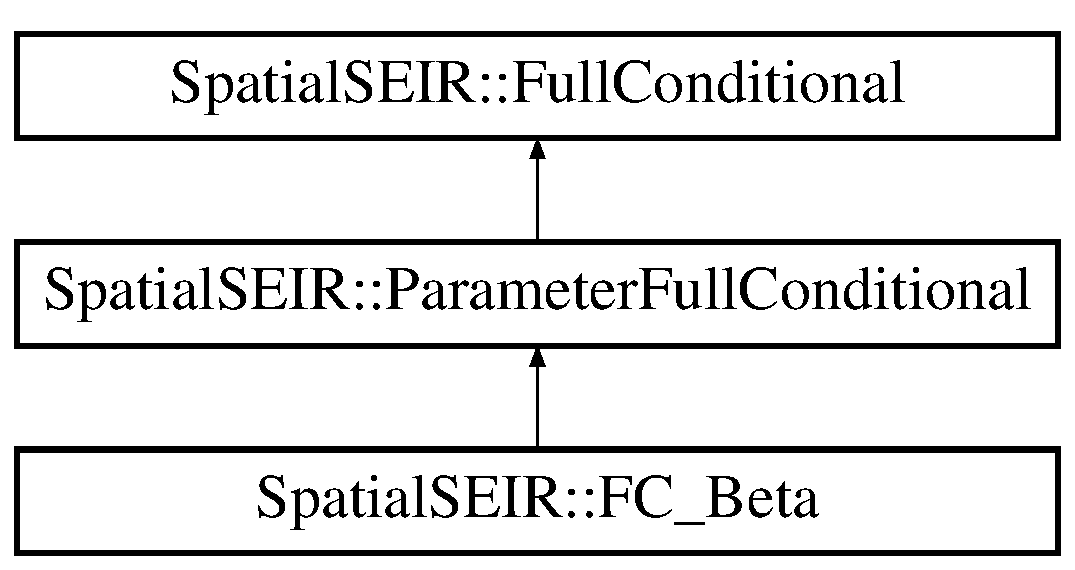
\includegraphics[height=3.000000cm]{classSpatialSEIR_1_1FC__Beta}
\end{center}
\end{figure}
\subsection*{Public Member Functions}
\begin{DoxyCompactItemize}
\item 
\hyperlink{classSpatialSEIR_1_1FC__Beta_a98918753da7fe5c3e7ae0de9a40cbf7d}{F\-C\-\_\-\-Beta} (\hyperlink{classSpatialSEIR_1_1ModelContext}{Model\-Context} $\ast$\-\_\-context, \hyperlink{classSpatialSEIR_1_1CompartmentalModelMatrix}{Compartmental\-Model\-Matrix} $\ast$\-\_\-\-E\-\_\-star, \hyperlink{classSpatialSEIR_1_1CompartmentalModelMatrix}{Compartmental\-Model\-Matrix} $\ast$\-\_\-\-S, \hyperlink{classSpatialSEIR_1_1InitData}{Init\-Data} $\ast$\-\_\-\-A0, \hyperlink{classSpatialSEIR_1_1CovariateMatrix}{Covariate\-Matrix} $\ast$\-\_\-\-X, double $\ast$\-\_\-p\-\_\-se, double $\ast$\-\_\-beta, double $\ast$\-\_\-rho, double \hyperlink{classSpatialSEIR_1_1FullConditional_a150ee031af8d086ad0a04b13630a110f}{slice\-Width}, double \-\_\-prior\-Precision)
\item 
\hyperlink{classSpatialSEIR_1_1FC__Beta_a47a6b14b1b441b9cd33ff8b59a644c44}{$\sim$\-F\-C\-\_\-\-Beta} ()
\item 
virtual double \hyperlink{classSpatialSEIR_1_1FC__Beta_a825ac001a023c64c6da372eedfae0e6e}{eval\-Prior} ()
\item 
virtual int \hyperlink{classSpatialSEIR_1_1FC__Beta_ae6f07bc7a0ef7ec660d1daadd060aad1}{eval\-C\-P\-U} ()
\item 
virtual int \hyperlink{classSpatialSEIR_1_1FC__Beta_a882c2de38ecfa3a425010874dfacda0f}{eval\-O\-C\-L} ()
\item 
virtual void \hyperlink{classSpatialSEIR_1_1FC__Beta_a96c2d002394eeee8cbcf7d06b8593dfc}{sample} (int verbose)
\item 
virtual long double \hyperlink{classSpatialSEIR_1_1FC__Beta_a3d25a7f6965f0a899249b76d8bd9d75f}{get\-Value} ()
\item 
virtual void \hyperlink{classSpatialSEIR_1_1FC__Beta_a545ac3e04204a54d6f34c4356f474e42}{set\-Value} (long double val)
\item 
virtual int \hyperlink{classSpatialSEIR_1_1FC__Beta_ae5a92d2c0ebd51328296a8db45fc52ad}{calculate\-Relevant\-Compartments} ()
\item 
virtual int \hyperlink{classSpatialSEIR_1_1FC__Beta_ac82fb2f313216cd5ebe611fbdf266416}{calculate\-Relevant\-Compartments\-\_\-\-O\-C\-L} ()
\end{DoxyCompactItemize}
\subsection*{Public Attributes}
\begin{DoxyCompactItemize}
\item 
\hyperlink{classSpatialSEIR_1_1ModelContext}{Model\-Context} $\ast$$\ast$ \hyperlink{classSpatialSEIR_1_1FC__Beta_abb49ac278509d42f38389f318fd372a7}{context}
\item 
\hyperlink{classSpatialSEIR_1_1CompartmentalModelMatrix}{Compartmental\-Model\-Matrix} $\ast$$\ast$ \hyperlink{classSpatialSEIR_1_1FC__Beta_a820c829d4e372e85b3afe3dbe1f9630f}{E\-\_\-star}
\item 
\hyperlink{classSpatialSEIR_1_1CompartmentalModelMatrix}{Compartmental\-Model\-Matrix} $\ast$$\ast$ \hyperlink{classSpatialSEIR_1_1FC__Beta_aaa946617743ffad43b73f7533c7fb6b5}{S}
\item 
\hyperlink{classSpatialSEIR_1_1InitData}{Init\-Data} $\ast$$\ast$ \hyperlink{classSpatialSEIR_1_1FC__Beta_aa17a045f03d452edba2242b3c2726e56}{A0}
\item 
\hyperlink{classSpatialSEIR_1_1CovariateMatrix}{Covariate\-Matrix} $\ast$$\ast$ \hyperlink{classSpatialSEIR_1_1FC__Beta_a3619f98f776ef5ab826350177e2f1326}{X}
\item 
double $\ast$$\ast$ \hyperlink{classSpatialSEIR_1_1FC__Beta_a6578a67debe1dbe47fff2f6c42ef865f}{p\-\_\-se}
\item 
double $\ast$$\ast$ \hyperlink{classSpatialSEIR_1_1FC__Beta_ad7d2994afbea485bb85f48901fda323f}{beta}
\item 
double $\ast$$\ast$ \hyperlink{classSpatialSEIR_1_1FC__Beta_a45c63ad745b312f58fba322223f78bbe}{rho}
\item 
long double $\ast$ \hyperlink{classSpatialSEIR_1_1FC__Beta_aae2fb964cd80bfa9eba448f2075640d5}{value}
\item 
double $\ast$ \hyperlink{classSpatialSEIR_1_1FC__Beta_a5f56c94d34e77cd4a331dfdcb169373e}{prior\-Precision}
\end{DoxyCompactItemize}


\subsection{Detailed Description}
\hyperlink{classSpatialSEIR_1_1FC__Beta}{F\-C\-\_\-\-Beta} gives the full conditional distribution of beta, the vector of regression parameters capturing the exposure intensity process. 

\subsection{Constructor \& Destructor Documentation}
\hypertarget{classSpatialSEIR_1_1FC__Beta_a98918753da7fe5c3e7ae0de9a40cbf7d}{\index{Spatial\-S\-E\-I\-R\-::\-F\-C\-\_\-\-Beta@{Spatial\-S\-E\-I\-R\-::\-F\-C\-\_\-\-Beta}!F\-C\-\_\-\-Beta@{F\-C\-\_\-\-Beta}}
\index{F\-C\-\_\-\-Beta@{F\-C\-\_\-\-Beta}!SpatialSEIR::FC_Beta@{Spatial\-S\-E\-I\-R\-::\-F\-C\-\_\-\-Beta}}
\subsubsection[{F\-C\-\_\-\-Beta}]{\setlength{\rightskip}{0pt plus 5cm}Spatial\-S\-E\-I\-R\-::\-F\-C\-\_\-\-Beta\-::\-F\-C\-\_\-\-Beta (
\begin{DoxyParamCaption}
\item[{{\bf Model\-Context} $\ast$}]{\-\_\-context, }
\item[{{\bf Compartmental\-Model\-Matrix} $\ast$}]{\-\_\-\-E\-\_\-star, }
\item[{{\bf Compartmental\-Model\-Matrix} $\ast$}]{\-\_\-\-S, }
\item[{{\bf Init\-Data} $\ast$}]{\-\_\-\-A0, }
\item[{{\bf Covariate\-Matrix} $\ast$}]{\-\_\-\-X, }
\item[{double $\ast$}]{\-\_\-p\-\_\-se, }
\item[{double $\ast$}]{\-\_\-beta, }
\item[{double $\ast$}]{\-\_\-rho, }
\item[{double}]{slice\-Width, }
\item[{double}]{\-\_\-prior\-Precision}
\end{DoxyParamCaption}
)}}\label{classSpatialSEIR_1_1FC__Beta_a98918753da7fe5c3e7ae0de9a40cbf7d}
\hypertarget{classSpatialSEIR_1_1FC__Beta_a47a6b14b1b441b9cd33ff8b59a644c44}{\index{Spatial\-S\-E\-I\-R\-::\-F\-C\-\_\-\-Beta@{Spatial\-S\-E\-I\-R\-::\-F\-C\-\_\-\-Beta}!$\sim$\-F\-C\-\_\-\-Beta@{$\sim$\-F\-C\-\_\-\-Beta}}
\index{$\sim$\-F\-C\-\_\-\-Beta@{$\sim$\-F\-C\-\_\-\-Beta}!SpatialSEIR::FC_Beta@{Spatial\-S\-E\-I\-R\-::\-F\-C\-\_\-\-Beta}}
\subsubsection[{$\sim$\-F\-C\-\_\-\-Beta}]{\setlength{\rightskip}{0pt plus 5cm}Spatial\-S\-E\-I\-R\-::\-F\-C\-\_\-\-Beta\-::$\sim$\-F\-C\-\_\-\-Beta (
\begin{DoxyParamCaption}
{}
\end{DoxyParamCaption}
)}}\label{classSpatialSEIR_1_1FC__Beta_a47a6b14b1b441b9cd33ff8b59a644c44}


\subsection{Member Function Documentation}
\hypertarget{classSpatialSEIR_1_1FC__Beta_ae5a92d2c0ebd51328296a8db45fc52ad}{\index{Spatial\-S\-E\-I\-R\-::\-F\-C\-\_\-\-Beta@{Spatial\-S\-E\-I\-R\-::\-F\-C\-\_\-\-Beta}!calculate\-Relevant\-Compartments@{calculate\-Relevant\-Compartments}}
\index{calculate\-Relevant\-Compartments@{calculate\-Relevant\-Compartments}!SpatialSEIR::FC_Beta@{Spatial\-S\-E\-I\-R\-::\-F\-C\-\_\-\-Beta}}
\subsubsection[{calculate\-Relevant\-Compartments}]{\setlength{\rightskip}{0pt plus 5cm}int Spatial\-S\-E\-I\-R\-::\-F\-C\-\_\-\-Beta\-::calculate\-Relevant\-Compartments (
\begin{DoxyParamCaption}
{}
\end{DoxyParamCaption}
)\hspace{0.3cm}{\ttfamily [virtual]}}}\label{classSpatialSEIR_1_1FC__Beta_ae5a92d2c0ebd51328296a8db45fc52ad}


Implements \hyperlink{classSpatialSEIR_1_1ParameterFullConditional_a65c39a2c3ca56e2f194b78cd362d35f9}{Spatial\-S\-E\-I\-R\-::\-Parameter\-Full\-Conditional}.

\hypertarget{classSpatialSEIR_1_1FC__Beta_ac82fb2f313216cd5ebe611fbdf266416}{\index{Spatial\-S\-E\-I\-R\-::\-F\-C\-\_\-\-Beta@{Spatial\-S\-E\-I\-R\-::\-F\-C\-\_\-\-Beta}!calculate\-Relevant\-Compartments\-\_\-\-O\-C\-L@{calculate\-Relevant\-Compartments\-\_\-\-O\-C\-L}}
\index{calculate\-Relevant\-Compartments\-\_\-\-O\-C\-L@{calculate\-Relevant\-Compartments\-\_\-\-O\-C\-L}!SpatialSEIR::FC_Beta@{Spatial\-S\-E\-I\-R\-::\-F\-C\-\_\-\-Beta}}
\subsubsection[{calculate\-Relevant\-Compartments\-\_\-\-O\-C\-L}]{\setlength{\rightskip}{0pt plus 5cm}int Spatial\-S\-E\-I\-R\-::\-F\-C\-\_\-\-Beta\-::calculate\-Relevant\-Compartments\-\_\-\-O\-C\-L (
\begin{DoxyParamCaption}
{}
\end{DoxyParamCaption}
)\hspace{0.3cm}{\ttfamily [virtual]}}}\label{classSpatialSEIR_1_1FC__Beta_ac82fb2f313216cd5ebe611fbdf266416}


Implements \hyperlink{classSpatialSEIR_1_1ParameterFullConditional_af40754537736a64f58848e0368b001fb}{Spatial\-S\-E\-I\-R\-::\-Parameter\-Full\-Conditional}.

\hypertarget{classSpatialSEIR_1_1FC__Beta_ae6f07bc7a0ef7ec660d1daadd060aad1}{\index{Spatial\-S\-E\-I\-R\-::\-F\-C\-\_\-\-Beta@{Spatial\-S\-E\-I\-R\-::\-F\-C\-\_\-\-Beta}!eval\-C\-P\-U@{eval\-C\-P\-U}}
\index{eval\-C\-P\-U@{eval\-C\-P\-U}!SpatialSEIR::FC_Beta@{Spatial\-S\-E\-I\-R\-::\-F\-C\-\_\-\-Beta}}
\subsubsection[{eval\-C\-P\-U}]{\setlength{\rightskip}{0pt plus 5cm}int Spatial\-S\-E\-I\-R\-::\-F\-C\-\_\-\-Beta\-::eval\-C\-P\-U (
\begin{DoxyParamCaption}
{}
\end{DoxyParamCaption}
)\hspace{0.3cm}{\ttfamily [virtual]}}}\label{classSpatialSEIR_1_1FC__Beta_ae6f07bc7a0ef7ec660d1daadd060aad1}


Implements \hyperlink{classSpatialSEIR_1_1ParameterFullConditional_a186bd19fdeb52ca4522f56fb880201dd}{Spatial\-S\-E\-I\-R\-::\-Parameter\-Full\-Conditional}.

\hypertarget{classSpatialSEIR_1_1FC__Beta_a882c2de38ecfa3a425010874dfacda0f}{\index{Spatial\-S\-E\-I\-R\-::\-F\-C\-\_\-\-Beta@{Spatial\-S\-E\-I\-R\-::\-F\-C\-\_\-\-Beta}!eval\-O\-C\-L@{eval\-O\-C\-L}}
\index{eval\-O\-C\-L@{eval\-O\-C\-L}!SpatialSEIR::FC_Beta@{Spatial\-S\-E\-I\-R\-::\-F\-C\-\_\-\-Beta}}
\subsubsection[{eval\-O\-C\-L}]{\setlength{\rightskip}{0pt plus 5cm}int Spatial\-S\-E\-I\-R\-::\-F\-C\-\_\-\-Beta\-::eval\-O\-C\-L (
\begin{DoxyParamCaption}
{}
\end{DoxyParamCaption}
)\hspace{0.3cm}{\ttfamily [virtual]}}}\label{classSpatialSEIR_1_1FC__Beta_a882c2de38ecfa3a425010874dfacda0f}


Implements \hyperlink{classSpatialSEIR_1_1ParameterFullConditional_ac4cfb13dace7f72e8136c45d9e959eec}{Spatial\-S\-E\-I\-R\-::\-Parameter\-Full\-Conditional}.

\hypertarget{classSpatialSEIR_1_1FC__Beta_a825ac001a023c64c6da372eedfae0e6e}{\index{Spatial\-S\-E\-I\-R\-::\-F\-C\-\_\-\-Beta@{Spatial\-S\-E\-I\-R\-::\-F\-C\-\_\-\-Beta}!eval\-Prior@{eval\-Prior}}
\index{eval\-Prior@{eval\-Prior}!SpatialSEIR::FC_Beta@{Spatial\-S\-E\-I\-R\-::\-F\-C\-\_\-\-Beta}}
\subsubsection[{eval\-Prior}]{\setlength{\rightskip}{0pt plus 5cm}double Spatial\-S\-E\-I\-R\-::\-F\-C\-\_\-\-Beta\-::eval\-Prior (
\begin{DoxyParamCaption}
{}
\end{DoxyParamCaption}
)\hspace{0.3cm}{\ttfamily [virtual]}}}\label{classSpatialSEIR_1_1FC__Beta_a825ac001a023c64c6da372eedfae0e6e}
\hypertarget{classSpatialSEIR_1_1FC__Beta_a3d25a7f6965f0a899249b76d8bd9d75f}{\index{Spatial\-S\-E\-I\-R\-::\-F\-C\-\_\-\-Beta@{Spatial\-S\-E\-I\-R\-::\-F\-C\-\_\-\-Beta}!get\-Value@{get\-Value}}
\index{get\-Value@{get\-Value}!SpatialSEIR::FC_Beta@{Spatial\-S\-E\-I\-R\-::\-F\-C\-\_\-\-Beta}}
\subsubsection[{get\-Value}]{\setlength{\rightskip}{0pt plus 5cm}long double Spatial\-S\-E\-I\-R\-::\-F\-C\-\_\-\-Beta\-::get\-Value (
\begin{DoxyParamCaption}
{}
\end{DoxyParamCaption}
)\hspace{0.3cm}{\ttfamily [virtual]}}}\label{classSpatialSEIR_1_1FC__Beta_a3d25a7f6965f0a899249b76d8bd9d75f}


Implements \hyperlink{classSpatialSEIR_1_1ParameterFullConditional_a901368d385809e77179b9fa7532adfec}{Spatial\-S\-E\-I\-R\-::\-Parameter\-Full\-Conditional}.

\hypertarget{classSpatialSEIR_1_1FC__Beta_a96c2d002394eeee8cbcf7d06b8593dfc}{\index{Spatial\-S\-E\-I\-R\-::\-F\-C\-\_\-\-Beta@{Spatial\-S\-E\-I\-R\-::\-F\-C\-\_\-\-Beta}!sample@{sample}}
\index{sample@{sample}!SpatialSEIR::FC_Beta@{Spatial\-S\-E\-I\-R\-::\-F\-C\-\_\-\-Beta}}
\subsubsection[{sample}]{\setlength{\rightskip}{0pt plus 5cm}void Spatial\-S\-E\-I\-R\-::\-F\-C\-\_\-\-Beta\-::sample (
\begin{DoxyParamCaption}
\item[{int}]{verbose}
\end{DoxyParamCaption}
)\hspace{0.3cm}{\ttfamily [virtual]}}}\label{classSpatialSEIR_1_1FC__Beta_a96c2d002394eeee8cbcf7d06b8593dfc}


Implements \hyperlink{classSpatialSEIR_1_1ParameterFullConditional_a651e22b15782acb6bd80be12bd476693}{Spatial\-S\-E\-I\-R\-::\-Parameter\-Full\-Conditional}.

\hypertarget{classSpatialSEIR_1_1FC__Beta_a545ac3e04204a54d6f34c4356f474e42}{\index{Spatial\-S\-E\-I\-R\-::\-F\-C\-\_\-\-Beta@{Spatial\-S\-E\-I\-R\-::\-F\-C\-\_\-\-Beta}!set\-Value@{set\-Value}}
\index{set\-Value@{set\-Value}!SpatialSEIR::FC_Beta@{Spatial\-S\-E\-I\-R\-::\-F\-C\-\_\-\-Beta}}
\subsubsection[{set\-Value}]{\setlength{\rightskip}{0pt plus 5cm}void Spatial\-S\-E\-I\-R\-::\-F\-C\-\_\-\-Beta\-::set\-Value (
\begin{DoxyParamCaption}
\item[{long double}]{val}
\end{DoxyParamCaption}
)\hspace{0.3cm}{\ttfamily [virtual]}}}\label{classSpatialSEIR_1_1FC__Beta_a545ac3e04204a54d6f34c4356f474e42}


Implements \hyperlink{classSpatialSEIR_1_1ParameterFullConditional_adf03f213e27d26f120b574d6dd86ffc3}{Spatial\-S\-E\-I\-R\-::\-Parameter\-Full\-Conditional}.



\subsection{Member Data Documentation}
\hypertarget{classSpatialSEIR_1_1FC__Beta_aa17a045f03d452edba2242b3c2726e56}{\index{Spatial\-S\-E\-I\-R\-::\-F\-C\-\_\-\-Beta@{Spatial\-S\-E\-I\-R\-::\-F\-C\-\_\-\-Beta}!A0@{A0}}
\index{A0@{A0}!SpatialSEIR::FC_Beta@{Spatial\-S\-E\-I\-R\-::\-F\-C\-\_\-\-Beta}}
\subsubsection[{A0}]{\setlength{\rightskip}{0pt plus 5cm}{\bf Init\-Data}$\ast$$\ast$ Spatial\-S\-E\-I\-R\-::\-F\-C\-\_\-\-Beta\-::\-A0}}\label{classSpatialSEIR_1_1FC__Beta_aa17a045f03d452edba2242b3c2726e56}
\hypertarget{classSpatialSEIR_1_1FC__Beta_ad7d2994afbea485bb85f48901fda323f}{\index{Spatial\-S\-E\-I\-R\-::\-F\-C\-\_\-\-Beta@{Spatial\-S\-E\-I\-R\-::\-F\-C\-\_\-\-Beta}!beta@{beta}}
\index{beta@{beta}!SpatialSEIR::FC_Beta@{Spatial\-S\-E\-I\-R\-::\-F\-C\-\_\-\-Beta}}
\subsubsection[{beta}]{\setlength{\rightskip}{0pt plus 5cm}double$\ast$$\ast$ Spatial\-S\-E\-I\-R\-::\-F\-C\-\_\-\-Beta\-::beta}}\label{classSpatialSEIR_1_1FC__Beta_ad7d2994afbea485bb85f48901fda323f}
\hypertarget{classSpatialSEIR_1_1FC__Beta_abb49ac278509d42f38389f318fd372a7}{\index{Spatial\-S\-E\-I\-R\-::\-F\-C\-\_\-\-Beta@{Spatial\-S\-E\-I\-R\-::\-F\-C\-\_\-\-Beta}!context@{context}}
\index{context@{context}!SpatialSEIR::FC_Beta@{Spatial\-S\-E\-I\-R\-::\-F\-C\-\_\-\-Beta}}
\subsubsection[{context}]{\setlength{\rightskip}{0pt plus 5cm}{\bf Model\-Context}$\ast$$\ast$ Spatial\-S\-E\-I\-R\-::\-F\-C\-\_\-\-Beta\-::context}}\label{classSpatialSEIR_1_1FC__Beta_abb49ac278509d42f38389f318fd372a7}
\hypertarget{classSpatialSEIR_1_1FC__Beta_a820c829d4e372e85b3afe3dbe1f9630f}{\index{Spatial\-S\-E\-I\-R\-::\-F\-C\-\_\-\-Beta@{Spatial\-S\-E\-I\-R\-::\-F\-C\-\_\-\-Beta}!E\-\_\-star@{E\-\_\-star}}
\index{E\-\_\-star@{E\-\_\-star}!SpatialSEIR::FC_Beta@{Spatial\-S\-E\-I\-R\-::\-F\-C\-\_\-\-Beta}}
\subsubsection[{E\-\_\-star}]{\setlength{\rightskip}{0pt plus 5cm}{\bf Compartmental\-Model\-Matrix}$\ast$$\ast$ Spatial\-S\-E\-I\-R\-::\-F\-C\-\_\-\-Beta\-::\-E\-\_\-star}}\label{classSpatialSEIR_1_1FC__Beta_a820c829d4e372e85b3afe3dbe1f9630f}
\hypertarget{classSpatialSEIR_1_1FC__Beta_a6578a67debe1dbe47fff2f6c42ef865f}{\index{Spatial\-S\-E\-I\-R\-::\-F\-C\-\_\-\-Beta@{Spatial\-S\-E\-I\-R\-::\-F\-C\-\_\-\-Beta}!p\-\_\-se@{p\-\_\-se}}
\index{p\-\_\-se@{p\-\_\-se}!SpatialSEIR::FC_Beta@{Spatial\-S\-E\-I\-R\-::\-F\-C\-\_\-\-Beta}}
\subsubsection[{p\-\_\-se}]{\setlength{\rightskip}{0pt plus 5cm}double$\ast$$\ast$ Spatial\-S\-E\-I\-R\-::\-F\-C\-\_\-\-Beta\-::p\-\_\-se}}\label{classSpatialSEIR_1_1FC__Beta_a6578a67debe1dbe47fff2f6c42ef865f}
\hypertarget{classSpatialSEIR_1_1FC__Beta_a5f56c94d34e77cd4a331dfdcb169373e}{\index{Spatial\-S\-E\-I\-R\-::\-F\-C\-\_\-\-Beta@{Spatial\-S\-E\-I\-R\-::\-F\-C\-\_\-\-Beta}!prior\-Precision@{prior\-Precision}}
\index{prior\-Precision@{prior\-Precision}!SpatialSEIR::FC_Beta@{Spatial\-S\-E\-I\-R\-::\-F\-C\-\_\-\-Beta}}
\subsubsection[{prior\-Precision}]{\setlength{\rightskip}{0pt plus 5cm}double$\ast$ Spatial\-S\-E\-I\-R\-::\-F\-C\-\_\-\-Beta\-::prior\-Precision}}\label{classSpatialSEIR_1_1FC__Beta_a5f56c94d34e77cd4a331dfdcb169373e}
\hypertarget{classSpatialSEIR_1_1FC__Beta_a45c63ad745b312f58fba322223f78bbe}{\index{Spatial\-S\-E\-I\-R\-::\-F\-C\-\_\-\-Beta@{Spatial\-S\-E\-I\-R\-::\-F\-C\-\_\-\-Beta}!rho@{rho}}
\index{rho@{rho}!SpatialSEIR::FC_Beta@{Spatial\-S\-E\-I\-R\-::\-F\-C\-\_\-\-Beta}}
\subsubsection[{rho}]{\setlength{\rightskip}{0pt plus 5cm}double$\ast$$\ast$ Spatial\-S\-E\-I\-R\-::\-F\-C\-\_\-\-Beta\-::rho}}\label{classSpatialSEIR_1_1FC__Beta_a45c63ad745b312f58fba322223f78bbe}
\hypertarget{classSpatialSEIR_1_1FC__Beta_aaa946617743ffad43b73f7533c7fb6b5}{\index{Spatial\-S\-E\-I\-R\-::\-F\-C\-\_\-\-Beta@{Spatial\-S\-E\-I\-R\-::\-F\-C\-\_\-\-Beta}!S@{S}}
\index{S@{S}!SpatialSEIR::FC_Beta@{Spatial\-S\-E\-I\-R\-::\-F\-C\-\_\-\-Beta}}
\subsubsection[{S}]{\setlength{\rightskip}{0pt plus 5cm}{\bf Compartmental\-Model\-Matrix}$\ast$$\ast$ Spatial\-S\-E\-I\-R\-::\-F\-C\-\_\-\-Beta\-::\-S}}\label{classSpatialSEIR_1_1FC__Beta_aaa946617743ffad43b73f7533c7fb6b5}
\hypertarget{classSpatialSEIR_1_1FC__Beta_aae2fb964cd80bfa9eba448f2075640d5}{\index{Spatial\-S\-E\-I\-R\-::\-F\-C\-\_\-\-Beta@{Spatial\-S\-E\-I\-R\-::\-F\-C\-\_\-\-Beta}!value@{value}}
\index{value@{value}!SpatialSEIR::FC_Beta@{Spatial\-S\-E\-I\-R\-::\-F\-C\-\_\-\-Beta}}
\subsubsection[{value}]{\setlength{\rightskip}{0pt plus 5cm}long double$\ast$ Spatial\-S\-E\-I\-R\-::\-F\-C\-\_\-\-Beta\-::value}}\label{classSpatialSEIR_1_1FC__Beta_aae2fb964cd80bfa9eba448f2075640d5}
\hypertarget{classSpatialSEIR_1_1FC__Beta_a3619f98f776ef5ab826350177e2f1326}{\index{Spatial\-S\-E\-I\-R\-::\-F\-C\-\_\-\-Beta@{Spatial\-S\-E\-I\-R\-::\-F\-C\-\_\-\-Beta}!X@{X}}
\index{X@{X}!SpatialSEIR::FC_Beta@{Spatial\-S\-E\-I\-R\-::\-F\-C\-\_\-\-Beta}}
\subsubsection[{X}]{\setlength{\rightskip}{0pt plus 5cm}{\bf Covariate\-Matrix}$\ast$$\ast$ Spatial\-S\-E\-I\-R\-::\-F\-C\-\_\-\-Beta\-::\-X}}\label{classSpatialSEIR_1_1FC__Beta_a3619f98f776ef5ab826350177e2f1326}


The documentation for this class was generated from the following files\-:\begin{DoxyCompactItemize}
\item 
lib\-Spatial\-S\-E\-I\-R/include/\-Full\-Conditionals/\hyperlink{LSS__FC__Beta_8hpp}{L\-S\-S\-\_\-\-F\-C\-\_\-\-Beta.\-hpp}\item 
lib\-Spatial\-S\-E\-I\-R/src/\-Full\-Conditionals/\hyperlink{FC__Beta_8cpp}{F\-C\-\_\-\-Beta.\-cpp}\end{DoxyCompactItemize}

\hypertarget{classSpatialSEIR_1_1FC__Beta__P__RS}{\section{Spatial\-S\-E\-I\-R\-:\-:F\-C\-\_\-\-Beta\-\_\-\-P\-\_\-\-R\-S Class Reference}
\label{classSpatialSEIR_1_1FC__Beta__P__RS}\index{Spatial\-S\-E\-I\-R\-::\-F\-C\-\_\-\-Beta\-\_\-\-P\-\_\-\-R\-S@{Spatial\-S\-E\-I\-R\-::\-F\-C\-\_\-\-Beta\-\_\-\-P\-\_\-\-R\-S}}
}


{\ttfamily \#include $<$L\-S\-S\-\_\-\-F\-C\-\_\-\-Beta\-\_\-\-P\-\_\-\-R\-S.\-hpp$>$}

Inheritance diagram for Spatial\-S\-E\-I\-R\-:\-:F\-C\-\_\-\-Beta\-\_\-\-P\-\_\-\-R\-S\-:\begin{figure}[H]
\begin{center}
\leavevmode
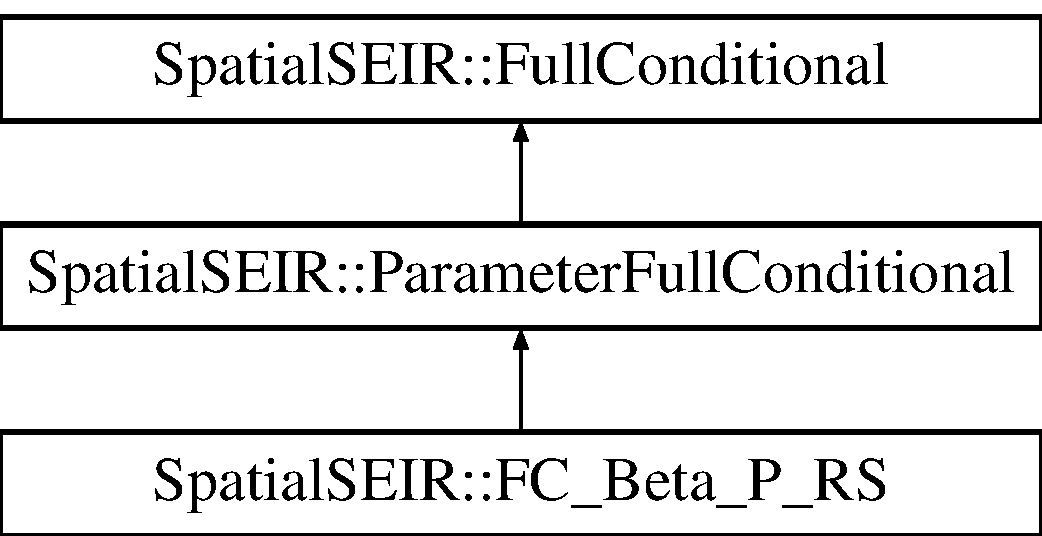
\includegraphics[height=3.000000cm]{classSpatialSEIR_1_1FC__Beta__P__RS}
\end{center}
\end{figure}
\subsection*{Public Member Functions}
\begin{DoxyCompactItemize}
\item 
\hyperlink{classSpatialSEIR_1_1FC__Beta__P__RS_ab39ed13b5740506c5b505ddc10127570}{F\-C\-\_\-\-Beta\-\_\-\-P\-\_\-\-R\-S} (\hyperlink{classSpatialSEIR_1_1ModelContext}{Model\-Context} $\ast$\-\_\-context, \hyperlink{classSpatialSEIR_1_1CompartmentalModelMatrix}{Compartmental\-Model\-Matrix} $\ast$\-\_\-\-S\-\_\-star, \hyperlink{classSpatialSEIR_1_1CompartmentalModelMatrix}{Compartmental\-Model\-Matrix} $\ast$\-\_\-\-R, \hyperlink{classSpatialSEIR_1_1CovariateMatrix}{Covariate\-Matrix} $\ast$\-\_\-\-X, \hyperlink{classSpatialSEIR_1_1InitData}{Init\-Data} $\ast$\-\_\-\-A0, double $\ast$\-\_\-p\-\_\-rs, double $\ast$\-\_\-beta\-\_\-p\-\_\-rs, double \-\_\-tausq, double \-\_\-slice\-Width)
\item 
\hyperlink{classSpatialSEIR_1_1FC__Beta__P__RS_afe2855aab7e504232715eb41ccc7be8c}{$\sim$\-F\-C\-\_\-\-Beta\-\_\-\-P\-\_\-\-R\-S} ()
\item 
virtual double \hyperlink{classSpatialSEIR_1_1FC__Beta__P__RS_af41981a47b1b923c1245329a871f28a9}{eval\-Prior} ()
\item 
virtual int \hyperlink{classSpatialSEIR_1_1FC__Beta__P__RS_a48e4e95be2abde217b71993c2b08e3da}{eval\-C\-P\-U} ()
\item 
virtual int \hyperlink{classSpatialSEIR_1_1FC__Beta__P__RS_ae51ca0e2ad990cd519fd62cf896c23ca}{eval\-O\-C\-L} ()
\item 
virtual void \hyperlink{classSpatialSEIR_1_1FC__Beta__P__RS_ae1a9ec2e9336c7c77106ff525d69ec64}{sample} (int verbose)
\item 
virtual long double \hyperlink{classSpatialSEIR_1_1FC__Beta__P__RS_a3017d4d02d954375869fe5d8e7e301ea}{get\-Value} ()
\item 
virtual void \hyperlink{classSpatialSEIR_1_1FC__Beta__P__RS_a788189d97ce2ffd40dc483a74ed63312}{set\-Value} (long double val)
\item 
virtual int \hyperlink{classSpatialSEIR_1_1FC__Beta__P__RS_a0edc8515a51962383536f8bf779ce194}{calculate\-Relevant\-Compartments} ()
\item 
virtual int \hyperlink{classSpatialSEIR_1_1FC__Beta__P__RS_a156069877b44b2d1b3ecd94bf019bf6d}{calculate\-Relevant\-Compartments\-\_\-\-O\-C\-L} ()
\end{DoxyCompactItemize}
\subsection*{Public Attributes}
\begin{DoxyCompactItemize}
\item 
\hyperlink{classSpatialSEIR_1_1ModelContext}{Model\-Context} $\ast$$\ast$ \hyperlink{classSpatialSEIR_1_1FC__Beta__P__RS_a5a34e90887bdaaf95426dd6aeffae6d5}{context}
\item 
\hyperlink{classSpatialSEIR_1_1CompartmentalModelMatrix}{Compartmental\-Model\-Matrix} $\ast$$\ast$ \hyperlink{classSpatialSEIR_1_1FC__Beta__P__RS_a4dea39caba374bb0ed9c1aa8d49c61cb}{S\-\_\-star}
\item 
\hyperlink{classSpatialSEIR_1_1CompartmentalModelMatrix}{Compartmental\-Model\-Matrix} $\ast$$\ast$ \hyperlink{classSpatialSEIR_1_1FC__Beta__P__RS_ad559b562d62e49e84fd737b001c887ef}{R}
\item 
\hyperlink{classSpatialSEIR_1_1CovariateMatrix}{Covariate\-Matrix} $\ast$$\ast$ \hyperlink{classSpatialSEIR_1_1FC__Beta__P__RS_a72f85c7949041f789c8a33cfd2e4f852}{X}
\item 
\hyperlink{classSpatialSEIR_1_1InitData}{Init\-Data} $\ast$$\ast$ \hyperlink{classSpatialSEIR_1_1FC__Beta__P__RS_a5ea17a82e1f860711f90db551b6412d8}{A0}
\item 
double $\ast$$\ast$ \hyperlink{classSpatialSEIR_1_1FC__Beta__P__RS_a57051ca845486c65fe38c42a55e3da5d}{beta\-\_\-p\-\_\-rs}
\item 
double $\ast$$\ast$ \hyperlink{classSpatialSEIR_1_1FC__Beta__P__RS_a69c39eb32b77b000c23e88259d01e913}{p\-\_\-rs}
\item 
double $\ast$ \hyperlink{classSpatialSEIR_1_1FC__Beta__P__RS_abbe3f96f9301c22e015cf7d16043b34c}{tausq}
\item 
long double $\ast$ \hyperlink{classSpatialSEIR_1_1FC__Beta__P__RS_af0841ebe767c583894eec3c3f4bcd3e9}{value}
\end{DoxyCompactItemize}


\subsection{Detailed Description}
\hyperlink{classSpatialSEIR_1_1FC__Beta__P__RS}{F\-C\-\_\-\-Beta\-\_\-\-P\-\_\-\-R\-S} gives the full conditional distribution of beta\-\_\-p\-\_\-rs, the vector of regression parameters capturing the probability that an individual transitions from R to S, the removed/recovered category to the susceptible category. 

\subsection{Constructor \& Destructor Documentation}
\hypertarget{classSpatialSEIR_1_1FC__Beta__P__RS_ab39ed13b5740506c5b505ddc10127570}{\index{Spatial\-S\-E\-I\-R\-::\-F\-C\-\_\-\-Beta\-\_\-\-P\-\_\-\-R\-S@{Spatial\-S\-E\-I\-R\-::\-F\-C\-\_\-\-Beta\-\_\-\-P\-\_\-\-R\-S}!F\-C\-\_\-\-Beta\-\_\-\-P\-\_\-\-R\-S@{F\-C\-\_\-\-Beta\-\_\-\-P\-\_\-\-R\-S}}
\index{F\-C\-\_\-\-Beta\-\_\-\-P\-\_\-\-R\-S@{F\-C\-\_\-\-Beta\-\_\-\-P\-\_\-\-R\-S}!SpatialSEIR::FC_Beta_P_RS@{Spatial\-S\-E\-I\-R\-::\-F\-C\-\_\-\-Beta\-\_\-\-P\-\_\-\-R\-S}}
\subsubsection[{F\-C\-\_\-\-Beta\-\_\-\-P\-\_\-\-R\-S}]{\setlength{\rightskip}{0pt plus 5cm}Spatial\-S\-E\-I\-R\-::\-F\-C\-\_\-\-Beta\-\_\-\-P\-\_\-\-R\-S\-::\-F\-C\-\_\-\-Beta\-\_\-\-P\-\_\-\-R\-S (
\begin{DoxyParamCaption}
\item[{{\bf Model\-Context} $\ast$}]{\-\_\-context, }
\item[{{\bf Compartmental\-Model\-Matrix} $\ast$}]{\-\_\-\-S\-\_\-star, }
\item[{{\bf Compartmental\-Model\-Matrix} $\ast$}]{\-\_\-\-R, }
\item[{{\bf Covariate\-Matrix} $\ast$}]{\-\_\-\-X, }
\item[{{\bf Init\-Data} $\ast$}]{\-\_\-\-A0, }
\item[{double $\ast$}]{\-\_\-p\-\_\-rs, }
\item[{double $\ast$}]{\-\_\-beta\-\_\-p\-\_\-rs, }
\item[{double}]{\-\_\-tausq, }
\item[{double}]{\-\_\-slice\-Width}
\end{DoxyParamCaption}
)}}\label{classSpatialSEIR_1_1FC__Beta__P__RS_ab39ed13b5740506c5b505ddc10127570}
\hypertarget{classSpatialSEIR_1_1FC__Beta__P__RS_afe2855aab7e504232715eb41ccc7be8c}{\index{Spatial\-S\-E\-I\-R\-::\-F\-C\-\_\-\-Beta\-\_\-\-P\-\_\-\-R\-S@{Spatial\-S\-E\-I\-R\-::\-F\-C\-\_\-\-Beta\-\_\-\-P\-\_\-\-R\-S}!$\sim$\-F\-C\-\_\-\-Beta\-\_\-\-P\-\_\-\-R\-S@{$\sim$\-F\-C\-\_\-\-Beta\-\_\-\-P\-\_\-\-R\-S}}
\index{$\sim$\-F\-C\-\_\-\-Beta\-\_\-\-P\-\_\-\-R\-S@{$\sim$\-F\-C\-\_\-\-Beta\-\_\-\-P\-\_\-\-R\-S}!SpatialSEIR::FC_Beta_P_RS@{Spatial\-S\-E\-I\-R\-::\-F\-C\-\_\-\-Beta\-\_\-\-P\-\_\-\-R\-S}}
\subsubsection[{$\sim$\-F\-C\-\_\-\-Beta\-\_\-\-P\-\_\-\-R\-S}]{\setlength{\rightskip}{0pt plus 5cm}Spatial\-S\-E\-I\-R\-::\-F\-C\-\_\-\-Beta\-\_\-\-P\-\_\-\-R\-S\-::$\sim$\-F\-C\-\_\-\-Beta\-\_\-\-P\-\_\-\-R\-S (
\begin{DoxyParamCaption}
{}
\end{DoxyParamCaption}
)}}\label{classSpatialSEIR_1_1FC__Beta__P__RS_afe2855aab7e504232715eb41ccc7be8c}


\subsection{Member Function Documentation}
\hypertarget{classSpatialSEIR_1_1FC__Beta__P__RS_a0edc8515a51962383536f8bf779ce194}{\index{Spatial\-S\-E\-I\-R\-::\-F\-C\-\_\-\-Beta\-\_\-\-P\-\_\-\-R\-S@{Spatial\-S\-E\-I\-R\-::\-F\-C\-\_\-\-Beta\-\_\-\-P\-\_\-\-R\-S}!calculate\-Relevant\-Compartments@{calculate\-Relevant\-Compartments}}
\index{calculate\-Relevant\-Compartments@{calculate\-Relevant\-Compartments}!SpatialSEIR::FC_Beta_P_RS@{Spatial\-S\-E\-I\-R\-::\-F\-C\-\_\-\-Beta\-\_\-\-P\-\_\-\-R\-S}}
\subsubsection[{calculate\-Relevant\-Compartments}]{\setlength{\rightskip}{0pt plus 5cm}int Spatial\-S\-E\-I\-R\-::\-F\-C\-\_\-\-Beta\-\_\-\-P\-\_\-\-R\-S\-::calculate\-Relevant\-Compartments (
\begin{DoxyParamCaption}
{}
\end{DoxyParamCaption}
)\hspace{0.3cm}{\ttfamily [virtual]}}}\label{classSpatialSEIR_1_1FC__Beta__P__RS_a0edc8515a51962383536f8bf779ce194}


Implements \hyperlink{classSpatialSEIR_1_1ParameterFullConditional_a65c39a2c3ca56e2f194b78cd362d35f9}{Spatial\-S\-E\-I\-R\-::\-Parameter\-Full\-Conditional}.

\hypertarget{classSpatialSEIR_1_1FC__Beta__P__RS_a156069877b44b2d1b3ecd94bf019bf6d}{\index{Spatial\-S\-E\-I\-R\-::\-F\-C\-\_\-\-Beta\-\_\-\-P\-\_\-\-R\-S@{Spatial\-S\-E\-I\-R\-::\-F\-C\-\_\-\-Beta\-\_\-\-P\-\_\-\-R\-S}!calculate\-Relevant\-Compartments\-\_\-\-O\-C\-L@{calculate\-Relevant\-Compartments\-\_\-\-O\-C\-L}}
\index{calculate\-Relevant\-Compartments\-\_\-\-O\-C\-L@{calculate\-Relevant\-Compartments\-\_\-\-O\-C\-L}!SpatialSEIR::FC_Beta_P_RS@{Spatial\-S\-E\-I\-R\-::\-F\-C\-\_\-\-Beta\-\_\-\-P\-\_\-\-R\-S}}
\subsubsection[{calculate\-Relevant\-Compartments\-\_\-\-O\-C\-L}]{\setlength{\rightskip}{0pt plus 5cm}int Spatial\-S\-E\-I\-R\-::\-F\-C\-\_\-\-Beta\-\_\-\-P\-\_\-\-R\-S\-::calculate\-Relevant\-Compartments\-\_\-\-O\-C\-L (
\begin{DoxyParamCaption}
{}
\end{DoxyParamCaption}
)\hspace{0.3cm}{\ttfamily [virtual]}}}\label{classSpatialSEIR_1_1FC__Beta__P__RS_a156069877b44b2d1b3ecd94bf019bf6d}


Implements \hyperlink{classSpatialSEIR_1_1ParameterFullConditional_af40754537736a64f58848e0368b001fb}{Spatial\-S\-E\-I\-R\-::\-Parameter\-Full\-Conditional}.

\hypertarget{classSpatialSEIR_1_1FC__Beta__P__RS_a48e4e95be2abde217b71993c2b08e3da}{\index{Spatial\-S\-E\-I\-R\-::\-F\-C\-\_\-\-Beta\-\_\-\-P\-\_\-\-R\-S@{Spatial\-S\-E\-I\-R\-::\-F\-C\-\_\-\-Beta\-\_\-\-P\-\_\-\-R\-S}!eval\-C\-P\-U@{eval\-C\-P\-U}}
\index{eval\-C\-P\-U@{eval\-C\-P\-U}!SpatialSEIR::FC_Beta_P_RS@{Spatial\-S\-E\-I\-R\-::\-F\-C\-\_\-\-Beta\-\_\-\-P\-\_\-\-R\-S}}
\subsubsection[{eval\-C\-P\-U}]{\setlength{\rightskip}{0pt plus 5cm}int Spatial\-S\-E\-I\-R\-::\-F\-C\-\_\-\-Beta\-\_\-\-P\-\_\-\-R\-S\-::eval\-C\-P\-U (
\begin{DoxyParamCaption}
{}
\end{DoxyParamCaption}
)\hspace{0.3cm}{\ttfamily [virtual]}}}\label{classSpatialSEIR_1_1FC__Beta__P__RS_a48e4e95be2abde217b71993c2b08e3da}


Implements \hyperlink{classSpatialSEIR_1_1ParameterFullConditional_a186bd19fdeb52ca4522f56fb880201dd}{Spatial\-S\-E\-I\-R\-::\-Parameter\-Full\-Conditional}.

\hypertarget{classSpatialSEIR_1_1FC__Beta__P__RS_ae51ca0e2ad990cd519fd62cf896c23ca}{\index{Spatial\-S\-E\-I\-R\-::\-F\-C\-\_\-\-Beta\-\_\-\-P\-\_\-\-R\-S@{Spatial\-S\-E\-I\-R\-::\-F\-C\-\_\-\-Beta\-\_\-\-P\-\_\-\-R\-S}!eval\-O\-C\-L@{eval\-O\-C\-L}}
\index{eval\-O\-C\-L@{eval\-O\-C\-L}!SpatialSEIR::FC_Beta_P_RS@{Spatial\-S\-E\-I\-R\-::\-F\-C\-\_\-\-Beta\-\_\-\-P\-\_\-\-R\-S}}
\subsubsection[{eval\-O\-C\-L}]{\setlength{\rightskip}{0pt plus 5cm}int Spatial\-S\-E\-I\-R\-::\-F\-C\-\_\-\-Beta\-\_\-\-P\-\_\-\-R\-S\-::eval\-O\-C\-L (
\begin{DoxyParamCaption}
{}
\end{DoxyParamCaption}
)\hspace{0.3cm}{\ttfamily [virtual]}}}\label{classSpatialSEIR_1_1FC__Beta__P__RS_ae51ca0e2ad990cd519fd62cf896c23ca}


Implements \hyperlink{classSpatialSEIR_1_1ParameterFullConditional_ac4cfb13dace7f72e8136c45d9e959eec}{Spatial\-S\-E\-I\-R\-::\-Parameter\-Full\-Conditional}.

\hypertarget{classSpatialSEIR_1_1FC__Beta__P__RS_af41981a47b1b923c1245329a871f28a9}{\index{Spatial\-S\-E\-I\-R\-::\-F\-C\-\_\-\-Beta\-\_\-\-P\-\_\-\-R\-S@{Spatial\-S\-E\-I\-R\-::\-F\-C\-\_\-\-Beta\-\_\-\-P\-\_\-\-R\-S}!eval\-Prior@{eval\-Prior}}
\index{eval\-Prior@{eval\-Prior}!SpatialSEIR::FC_Beta_P_RS@{Spatial\-S\-E\-I\-R\-::\-F\-C\-\_\-\-Beta\-\_\-\-P\-\_\-\-R\-S}}
\subsubsection[{eval\-Prior}]{\setlength{\rightskip}{0pt plus 5cm}double Spatial\-S\-E\-I\-R\-::\-F\-C\-\_\-\-Beta\-\_\-\-P\-\_\-\-R\-S\-::eval\-Prior (
\begin{DoxyParamCaption}
{}
\end{DoxyParamCaption}
)\hspace{0.3cm}{\ttfamily [virtual]}}}\label{classSpatialSEIR_1_1FC__Beta__P__RS_af41981a47b1b923c1245329a871f28a9}
\hypertarget{classSpatialSEIR_1_1FC__Beta__P__RS_a3017d4d02d954375869fe5d8e7e301ea}{\index{Spatial\-S\-E\-I\-R\-::\-F\-C\-\_\-\-Beta\-\_\-\-P\-\_\-\-R\-S@{Spatial\-S\-E\-I\-R\-::\-F\-C\-\_\-\-Beta\-\_\-\-P\-\_\-\-R\-S}!get\-Value@{get\-Value}}
\index{get\-Value@{get\-Value}!SpatialSEIR::FC_Beta_P_RS@{Spatial\-S\-E\-I\-R\-::\-F\-C\-\_\-\-Beta\-\_\-\-P\-\_\-\-R\-S}}
\subsubsection[{get\-Value}]{\setlength{\rightskip}{0pt plus 5cm}long double Spatial\-S\-E\-I\-R\-::\-F\-C\-\_\-\-Beta\-\_\-\-P\-\_\-\-R\-S\-::get\-Value (
\begin{DoxyParamCaption}
{}
\end{DoxyParamCaption}
)\hspace{0.3cm}{\ttfamily [virtual]}}}\label{classSpatialSEIR_1_1FC__Beta__P__RS_a3017d4d02d954375869fe5d8e7e301ea}


Implements \hyperlink{classSpatialSEIR_1_1ParameterFullConditional_a901368d385809e77179b9fa7532adfec}{Spatial\-S\-E\-I\-R\-::\-Parameter\-Full\-Conditional}.

\hypertarget{classSpatialSEIR_1_1FC__Beta__P__RS_ae1a9ec2e9336c7c77106ff525d69ec64}{\index{Spatial\-S\-E\-I\-R\-::\-F\-C\-\_\-\-Beta\-\_\-\-P\-\_\-\-R\-S@{Spatial\-S\-E\-I\-R\-::\-F\-C\-\_\-\-Beta\-\_\-\-P\-\_\-\-R\-S}!sample@{sample}}
\index{sample@{sample}!SpatialSEIR::FC_Beta_P_RS@{Spatial\-S\-E\-I\-R\-::\-F\-C\-\_\-\-Beta\-\_\-\-P\-\_\-\-R\-S}}
\subsubsection[{sample}]{\setlength{\rightskip}{0pt plus 5cm}void Spatial\-S\-E\-I\-R\-::\-F\-C\-\_\-\-Beta\-\_\-\-P\-\_\-\-R\-S\-::sample (
\begin{DoxyParamCaption}
\item[{int}]{verbose}
\end{DoxyParamCaption}
)\hspace{0.3cm}{\ttfamily [virtual]}}}\label{classSpatialSEIR_1_1FC__Beta__P__RS_ae1a9ec2e9336c7c77106ff525d69ec64}


Implements \hyperlink{classSpatialSEIR_1_1ParameterFullConditional_a651e22b15782acb6bd80be12bd476693}{Spatial\-S\-E\-I\-R\-::\-Parameter\-Full\-Conditional}.

\hypertarget{classSpatialSEIR_1_1FC__Beta__P__RS_a788189d97ce2ffd40dc483a74ed63312}{\index{Spatial\-S\-E\-I\-R\-::\-F\-C\-\_\-\-Beta\-\_\-\-P\-\_\-\-R\-S@{Spatial\-S\-E\-I\-R\-::\-F\-C\-\_\-\-Beta\-\_\-\-P\-\_\-\-R\-S}!set\-Value@{set\-Value}}
\index{set\-Value@{set\-Value}!SpatialSEIR::FC_Beta_P_RS@{Spatial\-S\-E\-I\-R\-::\-F\-C\-\_\-\-Beta\-\_\-\-P\-\_\-\-R\-S}}
\subsubsection[{set\-Value}]{\setlength{\rightskip}{0pt plus 5cm}void Spatial\-S\-E\-I\-R\-::\-F\-C\-\_\-\-Beta\-\_\-\-P\-\_\-\-R\-S\-::set\-Value (
\begin{DoxyParamCaption}
\item[{long double}]{val}
\end{DoxyParamCaption}
)\hspace{0.3cm}{\ttfamily [virtual]}}}\label{classSpatialSEIR_1_1FC__Beta__P__RS_a788189d97ce2ffd40dc483a74ed63312}


Implements \hyperlink{classSpatialSEIR_1_1ParameterFullConditional_adf03f213e27d26f120b574d6dd86ffc3}{Spatial\-S\-E\-I\-R\-::\-Parameter\-Full\-Conditional}.



\subsection{Member Data Documentation}
\hypertarget{classSpatialSEIR_1_1FC__Beta__P__RS_a5ea17a82e1f860711f90db551b6412d8}{\index{Spatial\-S\-E\-I\-R\-::\-F\-C\-\_\-\-Beta\-\_\-\-P\-\_\-\-R\-S@{Spatial\-S\-E\-I\-R\-::\-F\-C\-\_\-\-Beta\-\_\-\-P\-\_\-\-R\-S}!A0@{A0}}
\index{A0@{A0}!SpatialSEIR::FC_Beta_P_RS@{Spatial\-S\-E\-I\-R\-::\-F\-C\-\_\-\-Beta\-\_\-\-P\-\_\-\-R\-S}}
\subsubsection[{A0}]{\setlength{\rightskip}{0pt plus 5cm}{\bf Init\-Data}$\ast$$\ast$ Spatial\-S\-E\-I\-R\-::\-F\-C\-\_\-\-Beta\-\_\-\-P\-\_\-\-R\-S\-::\-A0}}\label{classSpatialSEIR_1_1FC__Beta__P__RS_a5ea17a82e1f860711f90db551b6412d8}
\hypertarget{classSpatialSEIR_1_1FC__Beta__P__RS_a57051ca845486c65fe38c42a55e3da5d}{\index{Spatial\-S\-E\-I\-R\-::\-F\-C\-\_\-\-Beta\-\_\-\-P\-\_\-\-R\-S@{Spatial\-S\-E\-I\-R\-::\-F\-C\-\_\-\-Beta\-\_\-\-P\-\_\-\-R\-S}!beta\-\_\-p\-\_\-rs@{beta\-\_\-p\-\_\-rs}}
\index{beta\-\_\-p\-\_\-rs@{beta\-\_\-p\-\_\-rs}!SpatialSEIR::FC_Beta_P_RS@{Spatial\-S\-E\-I\-R\-::\-F\-C\-\_\-\-Beta\-\_\-\-P\-\_\-\-R\-S}}
\subsubsection[{beta\-\_\-p\-\_\-rs}]{\setlength{\rightskip}{0pt plus 5cm}double$\ast$$\ast$ Spatial\-S\-E\-I\-R\-::\-F\-C\-\_\-\-Beta\-\_\-\-P\-\_\-\-R\-S\-::beta\-\_\-p\-\_\-rs}}\label{classSpatialSEIR_1_1FC__Beta__P__RS_a57051ca845486c65fe38c42a55e3da5d}
\hypertarget{classSpatialSEIR_1_1FC__Beta__P__RS_a5a34e90887bdaaf95426dd6aeffae6d5}{\index{Spatial\-S\-E\-I\-R\-::\-F\-C\-\_\-\-Beta\-\_\-\-P\-\_\-\-R\-S@{Spatial\-S\-E\-I\-R\-::\-F\-C\-\_\-\-Beta\-\_\-\-P\-\_\-\-R\-S}!context@{context}}
\index{context@{context}!SpatialSEIR::FC_Beta_P_RS@{Spatial\-S\-E\-I\-R\-::\-F\-C\-\_\-\-Beta\-\_\-\-P\-\_\-\-R\-S}}
\subsubsection[{context}]{\setlength{\rightskip}{0pt plus 5cm}{\bf Model\-Context}$\ast$$\ast$ Spatial\-S\-E\-I\-R\-::\-F\-C\-\_\-\-Beta\-\_\-\-P\-\_\-\-R\-S\-::context}}\label{classSpatialSEIR_1_1FC__Beta__P__RS_a5a34e90887bdaaf95426dd6aeffae6d5}
\hypertarget{classSpatialSEIR_1_1FC__Beta__P__RS_a69c39eb32b77b000c23e88259d01e913}{\index{Spatial\-S\-E\-I\-R\-::\-F\-C\-\_\-\-Beta\-\_\-\-P\-\_\-\-R\-S@{Spatial\-S\-E\-I\-R\-::\-F\-C\-\_\-\-Beta\-\_\-\-P\-\_\-\-R\-S}!p\-\_\-rs@{p\-\_\-rs}}
\index{p\-\_\-rs@{p\-\_\-rs}!SpatialSEIR::FC_Beta_P_RS@{Spatial\-S\-E\-I\-R\-::\-F\-C\-\_\-\-Beta\-\_\-\-P\-\_\-\-R\-S}}
\subsubsection[{p\-\_\-rs}]{\setlength{\rightskip}{0pt plus 5cm}double$\ast$$\ast$ Spatial\-S\-E\-I\-R\-::\-F\-C\-\_\-\-Beta\-\_\-\-P\-\_\-\-R\-S\-::p\-\_\-rs}}\label{classSpatialSEIR_1_1FC__Beta__P__RS_a69c39eb32b77b000c23e88259d01e913}
\hypertarget{classSpatialSEIR_1_1FC__Beta__P__RS_ad559b562d62e49e84fd737b001c887ef}{\index{Spatial\-S\-E\-I\-R\-::\-F\-C\-\_\-\-Beta\-\_\-\-P\-\_\-\-R\-S@{Spatial\-S\-E\-I\-R\-::\-F\-C\-\_\-\-Beta\-\_\-\-P\-\_\-\-R\-S}!R@{R}}
\index{R@{R}!SpatialSEIR::FC_Beta_P_RS@{Spatial\-S\-E\-I\-R\-::\-F\-C\-\_\-\-Beta\-\_\-\-P\-\_\-\-R\-S}}
\subsubsection[{R}]{\setlength{\rightskip}{0pt plus 5cm}{\bf Compartmental\-Model\-Matrix}$\ast$$\ast$ Spatial\-S\-E\-I\-R\-::\-F\-C\-\_\-\-Beta\-\_\-\-P\-\_\-\-R\-S\-::\-R}}\label{classSpatialSEIR_1_1FC__Beta__P__RS_ad559b562d62e49e84fd737b001c887ef}
\hypertarget{classSpatialSEIR_1_1FC__Beta__P__RS_a4dea39caba374bb0ed9c1aa8d49c61cb}{\index{Spatial\-S\-E\-I\-R\-::\-F\-C\-\_\-\-Beta\-\_\-\-P\-\_\-\-R\-S@{Spatial\-S\-E\-I\-R\-::\-F\-C\-\_\-\-Beta\-\_\-\-P\-\_\-\-R\-S}!S\-\_\-star@{S\-\_\-star}}
\index{S\-\_\-star@{S\-\_\-star}!SpatialSEIR::FC_Beta_P_RS@{Spatial\-S\-E\-I\-R\-::\-F\-C\-\_\-\-Beta\-\_\-\-P\-\_\-\-R\-S}}
\subsubsection[{S\-\_\-star}]{\setlength{\rightskip}{0pt plus 5cm}{\bf Compartmental\-Model\-Matrix}$\ast$$\ast$ Spatial\-S\-E\-I\-R\-::\-F\-C\-\_\-\-Beta\-\_\-\-P\-\_\-\-R\-S\-::\-S\-\_\-star}}\label{classSpatialSEIR_1_1FC__Beta__P__RS_a4dea39caba374bb0ed9c1aa8d49c61cb}
\hypertarget{classSpatialSEIR_1_1FC__Beta__P__RS_abbe3f96f9301c22e015cf7d16043b34c}{\index{Spatial\-S\-E\-I\-R\-::\-F\-C\-\_\-\-Beta\-\_\-\-P\-\_\-\-R\-S@{Spatial\-S\-E\-I\-R\-::\-F\-C\-\_\-\-Beta\-\_\-\-P\-\_\-\-R\-S}!tausq@{tausq}}
\index{tausq@{tausq}!SpatialSEIR::FC_Beta_P_RS@{Spatial\-S\-E\-I\-R\-::\-F\-C\-\_\-\-Beta\-\_\-\-P\-\_\-\-R\-S}}
\subsubsection[{tausq}]{\setlength{\rightskip}{0pt plus 5cm}double$\ast$ Spatial\-S\-E\-I\-R\-::\-F\-C\-\_\-\-Beta\-\_\-\-P\-\_\-\-R\-S\-::tausq}}\label{classSpatialSEIR_1_1FC__Beta__P__RS_abbe3f96f9301c22e015cf7d16043b34c}
\hypertarget{classSpatialSEIR_1_1FC__Beta__P__RS_af0841ebe767c583894eec3c3f4bcd3e9}{\index{Spatial\-S\-E\-I\-R\-::\-F\-C\-\_\-\-Beta\-\_\-\-P\-\_\-\-R\-S@{Spatial\-S\-E\-I\-R\-::\-F\-C\-\_\-\-Beta\-\_\-\-P\-\_\-\-R\-S}!value@{value}}
\index{value@{value}!SpatialSEIR::FC_Beta_P_RS@{Spatial\-S\-E\-I\-R\-::\-F\-C\-\_\-\-Beta\-\_\-\-P\-\_\-\-R\-S}}
\subsubsection[{value}]{\setlength{\rightskip}{0pt plus 5cm}long double$\ast$ Spatial\-S\-E\-I\-R\-::\-F\-C\-\_\-\-Beta\-\_\-\-P\-\_\-\-R\-S\-::value}}\label{classSpatialSEIR_1_1FC__Beta__P__RS_af0841ebe767c583894eec3c3f4bcd3e9}
\hypertarget{classSpatialSEIR_1_1FC__Beta__P__RS_a72f85c7949041f789c8a33cfd2e4f852}{\index{Spatial\-S\-E\-I\-R\-::\-F\-C\-\_\-\-Beta\-\_\-\-P\-\_\-\-R\-S@{Spatial\-S\-E\-I\-R\-::\-F\-C\-\_\-\-Beta\-\_\-\-P\-\_\-\-R\-S}!X@{X}}
\index{X@{X}!SpatialSEIR::FC_Beta_P_RS@{Spatial\-S\-E\-I\-R\-::\-F\-C\-\_\-\-Beta\-\_\-\-P\-\_\-\-R\-S}}
\subsubsection[{X}]{\setlength{\rightskip}{0pt plus 5cm}{\bf Covariate\-Matrix}$\ast$$\ast$ Spatial\-S\-E\-I\-R\-::\-F\-C\-\_\-\-Beta\-\_\-\-P\-\_\-\-R\-S\-::\-X}}\label{classSpatialSEIR_1_1FC__Beta__P__RS_a72f85c7949041f789c8a33cfd2e4f852}


The documentation for this class was generated from the following files\-:\begin{DoxyCompactItemize}
\item 
lib\-Spatial\-S\-E\-I\-R/include/\-Full\-Conditionals/\hyperlink{LSS__FC__Beta__P__RS_8hpp}{L\-S\-S\-\_\-\-F\-C\-\_\-\-Beta\-\_\-\-P\-\_\-\-R\-S.\-hpp}\item 
lib\-Spatial\-S\-E\-I\-R/src/\-Full\-Conditionals/\hyperlink{FC__Beta__P__RS_8cpp}{F\-C\-\_\-\-Beta\-\_\-\-P\-\_\-\-R\-S.\-cpp}\end{DoxyCompactItemize}

\hypertarget{classSpatialSEIR_1_1FC__E0}{\section{Spatial\-S\-E\-I\-R\-:\-:F\-C\-\_\-\-E0 Class Reference}
\label{classSpatialSEIR_1_1FC__E0}\index{Spatial\-S\-E\-I\-R\-::\-F\-C\-\_\-\-E0@{Spatial\-S\-E\-I\-R\-::\-F\-C\-\_\-\-E0}}
}


{\ttfamily \#include $<$L\-S\-S\-\_\-\-F\-C\-\_\-\-E0.\-hpp$>$}

Inheritance diagram for Spatial\-S\-E\-I\-R\-:\-:F\-C\-\_\-\-E0\-:\begin{figure}[H]
\begin{center}
\leavevmode
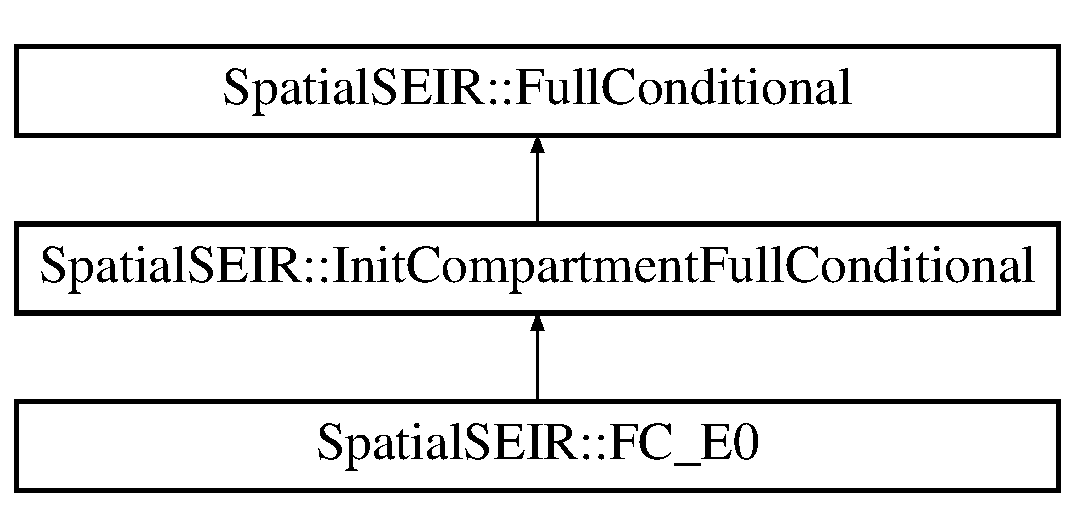
\includegraphics[height=3.000000cm]{classSpatialSEIR_1_1FC__E0}
\end{center}
\end{figure}
\subsection*{Public Member Functions}
\begin{DoxyCompactItemize}
\item 
\hyperlink{classSpatialSEIR_1_1FC__E0_af49361f736866374bc4d7c568c443da7}{F\-C\-\_\-\-E0} (\hyperlink{classSpatialSEIR_1_1ModelContext}{Model\-Context} $\ast$\-\_\-context, \hyperlink{classSpatialSEIR_1_1CompartmentalModelMatrix}{Compartmental\-Model\-Matrix} $\ast$\-\_\-\-S, \hyperlink{classSpatialSEIR_1_1CompartmentalModelMatrix}{Compartmental\-Model\-Matrix} $\ast$\-\_\-\-E, \hyperlink{classSpatialSEIR_1_1CompartmentalModelMatrix}{Compartmental\-Model\-Matrix} $\ast$\-\_\-\-I, \hyperlink{classSpatialSEIR_1_1CompartmentalModelMatrix}{Compartmental\-Model\-Matrix} $\ast$\-\_\-\-E\-\_\-star, \hyperlink{classSpatialSEIR_1_1CompartmentalModelMatrix}{Compartmental\-Model\-Matrix} $\ast$\-\_\-\-I\-\_\-star, \hyperlink{classSpatialSEIR_1_1CompartmentalModelMatrix}{Compartmental\-Model\-Matrix} $\ast$\-\_\-\-R\-\_\-star, \hyperlink{classSpatialSEIR_1_1InitData}{Init\-Data} $\ast$\-\_\-\-A0, double $\ast$\-\_\-p\-\_\-ir, double $\ast$\-\_\-p\-\_\-ei, double $\ast$\-\_\-p\-\_\-se, double \hyperlink{classSpatialSEIR_1_1FullConditional_a150ee031af8d086ad0a04b13630a110f}{slice\-Width})
\item 
virtual \hyperlink{classSpatialSEIR_1_1FC__E0_adc32c559bbb774d1c361a4f830856cb1}{$\sim$\-F\-C\-\_\-\-E0} ()
\item 
virtual int \hyperlink{classSpatialSEIR_1_1FC__E0_a6f38f6b04084d8cc9a94a360195e459c}{eval\-C\-P\-U} ()
\item 
virtual int \hyperlink{classSpatialSEIR_1_1FC__E0_a7470507101e662f3f0c1b1a6ab861089}{eval\-O\-C\-L} ()
\item 
virtual void \hyperlink{classSpatialSEIR_1_1FC__E0_a7b396dca06e12a96473d3bf2855a9dc7}{sample} (int verbose)
\item 
virtual long double \hyperlink{classSpatialSEIR_1_1FC__E0_aa2681b2dc4378d162dd2c68ff5333288}{get\-Value} ()
\item 
virtual void \hyperlink{classSpatialSEIR_1_1FC__E0_a44355906ac90df5dff3e0b7ffc62e23b}{set\-Value} (long double \hyperlink{classSpatialSEIR_1_1FC__E0_a79d0c47dfdb185a65082c6685cd5b149}{value})
\item 
virtual int \hyperlink{classSpatialSEIR_1_1FC__E0_accae19c302cdd306fdfebf3a76c84c11}{calculate\-Relevant\-Compartments} ()
\item 
virtual int \hyperlink{classSpatialSEIR_1_1FC__E0_aab40abc211ff8095a6ed0ec0b0c48b51}{calculate\-Relevant\-Compartments\-\_\-\-O\-C\-L} ()
\end{DoxyCompactItemize}
\subsection*{Public Attributes}
\begin{DoxyCompactItemize}
\item 
\hyperlink{classSpatialSEIR_1_1ModelContext}{Model\-Context} $\ast$$\ast$ \hyperlink{classSpatialSEIR_1_1FC__E0_ace226479b2a1d21777d489e7ff23a395}{context}
\item 
\hyperlink{classSpatialSEIR_1_1CompartmentalModelMatrix}{Compartmental\-Model\-Matrix} $\ast$$\ast$ \hyperlink{classSpatialSEIR_1_1FC__E0_a53998232503fd25c9d74d5c31867cbb9}{S}
\item 
\hyperlink{classSpatialSEIR_1_1CompartmentalModelMatrix}{Compartmental\-Model\-Matrix} $\ast$$\ast$ \hyperlink{classSpatialSEIR_1_1FC__E0_a5e58c11a403f3ed5e8d81710d8381d6a}{E}
\item 
\hyperlink{classSpatialSEIR_1_1CompartmentalModelMatrix}{Compartmental\-Model\-Matrix} $\ast$$\ast$ \hyperlink{classSpatialSEIR_1_1FC__E0_a048432b716d928e7ad3d2d58d448139d}{I}
\item 
\hyperlink{classSpatialSEIR_1_1CompartmentalModelMatrix}{Compartmental\-Model\-Matrix} $\ast$$\ast$ \hyperlink{classSpatialSEIR_1_1FC__E0_aed54e3f0f64667ca2624993257533c25}{E\-\_\-star}
\item 
\hyperlink{classSpatialSEIR_1_1CompartmentalModelMatrix}{Compartmental\-Model\-Matrix} $\ast$$\ast$ \hyperlink{classSpatialSEIR_1_1FC__E0_a5a40eb8abec5db63710a0d84bdad151c}{I\-\_\-star}
\item 
\hyperlink{classSpatialSEIR_1_1CompartmentalModelMatrix}{Compartmental\-Model\-Matrix} $\ast$$\ast$ \hyperlink{classSpatialSEIR_1_1FC__E0_a52c3029c4bf92c378524af2ac180b7c9}{R\-\_\-star}
\item 
\hyperlink{classSpatialSEIR_1_1InitData}{Init\-Data} $\ast$$\ast$ \hyperlink{classSpatialSEIR_1_1FC__E0_af28adc565332fd8e2e3a38e50b7ca182}{A0}
\item 
double $\ast$$\ast$ \hyperlink{classSpatialSEIR_1_1FC__E0_a738e723abd63fed586a769bcbee15d88}{p\-\_\-se}
\item 
double $\ast$$\ast$ \hyperlink{classSpatialSEIR_1_1FC__E0_a69ba193a361160f0ede692f2022d7621}{p\-\_\-ir}
\item 
double $\ast$$\ast$ \hyperlink{classSpatialSEIR_1_1FC__E0_a7d1dafac2b00d11e9b44f94934606621}{p\-\_\-ei}
\item 
long double $\ast$ \hyperlink{classSpatialSEIR_1_1FC__E0_a79d0c47dfdb185a65082c6685cd5b149}{value}
\end{DoxyCompactItemize}


\subsection{Detailed Description}
\hyperlink{classSpatialSEIR_1_1FC__E0}{F\-C\-\_\-\-E0} gives the full conditional distribution for the vector of initially exposed individuals. 

\subsection{Constructor \& Destructor Documentation}
\hypertarget{classSpatialSEIR_1_1FC__E0_af49361f736866374bc4d7c568c443da7}{\index{Spatial\-S\-E\-I\-R\-::\-F\-C\-\_\-\-E0@{Spatial\-S\-E\-I\-R\-::\-F\-C\-\_\-\-E0}!F\-C\-\_\-\-E0@{F\-C\-\_\-\-E0}}
\index{F\-C\-\_\-\-E0@{F\-C\-\_\-\-E0}!SpatialSEIR::FC_E0@{Spatial\-S\-E\-I\-R\-::\-F\-C\-\_\-\-E0}}
\subsubsection[{F\-C\-\_\-\-E0}]{\setlength{\rightskip}{0pt plus 5cm}Spatial\-S\-E\-I\-R\-::\-F\-C\-\_\-\-E0\-::\-F\-C\-\_\-\-E0 (
\begin{DoxyParamCaption}
\item[{{\bf Model\-Context} $\ast$}]{\-\_\-context, }
\item[{{\bf Compartmental\-Model\-Matrix} $\ast$}]{\-\_\-\-S, }
\item[{{\bf Compartmental\-Model\-Matrix} $\ast$}]{\-\_\-\-E, }
\item[{{\bf Compartmental\-Model\-Matrix} $\ast$}]{\-\_\-\-I, }
\item[{{\bf Compartmental\-Model\-Matrix} $\ast$}]{\-\_\-\-E\-\_\-star, }
\item[{{\bf Compartmental\-Model\-Matrix} $\ast$}]{\-\_\-\-I\-\_\-star, }
\item[{{\bf Compartmental\-Model\-Matrix} $\ast$}]{\-\_\-\-R\-\_\-star, }
\item[{{\bf Init\-Data} $\ast$}]{\-\_\-\-A0, }
\item[{double $\ast$}]{\-\_\-p\-\_\-ir, }
\item[{double $\ast$}]{\-\_\-p\-\_\-ei, }
\item[{double $\ast$}]{\-\_\-p\-\_\-se, }
\item[{double}]{slice\-Width}
\end{DoxyParamCaption}
)}}\label{classSpatialSEIR_1_1FC__E0_af49361f736866374bc4d7c568c443da7}
\hypertarget{classSpatialSEIR_1_1FC__E0_adc32c559bbb774d1c361a4f830856cb1}{\index{Spatial\-S\-E\-I\-R\-::\-F\-C\-\_\-\-E0@{Spatial\-S\-E\-I\-R\-::\-F\-C\-\_\-\-E0}!$\sim$\-F\-C\-\_\-\-E0@{$\sim$\-F\-C\-\_\-\-E0}}
\index{$\sim$\-F\-C\-\_\-\-E0@{$\sim$\-F\-C\-\_\-\-E0}!SpatialSEIR::FC_E0@{Spatial\-S\-E\-I\-R\-::\-F\-C\-\_\-\-E0}}
\subsubsection[{$\sim$\-F\-C\-\_\-\-E0}]{\setlength{\rightskip}{0pt plus 5cm}Spatial\-S\-E\-I\-R\-::\-F\-C\-\_\-\-E0\-::$\sim$\-F\-C\-\_\-\-E0 (
\begin{DoxyParamCaption}
{}
\end{DoxyParamCaption}
)\hspace{0.3cm}{\ttfamily [virtual]}}}\label{classSpatialSEIR_1_1FC__E0_adc32c559bbb774d1c361a4f830856cb1}


\subsection{Member Function Documentation}
\hypertarget{classSpatialSEIR_1_1FC__E0_accae19c302cdd306fdfebf3a76c84c11}{\index{Spatial\-S\-E\-I\-R\-::\-F\-C\-\_\-\-E0@{Spatial\-S\-E\-I\-R\-::\-F\-C\-\_\-\-E0}!calculate\-Relevant\-Compartments@{calculate\-Relevant\-Compartments}}
\index{calculate\-Relevant\-Compartments@{calculate\-Relevant\-Compartments}!SpatialSEIR::FC_E0@{Spatial\-S\-E\-I\-R\-::\-F\-C\-\_\-\-E0}}
\subsubsection[{calculate\-Relevant\-Compartments}]{\setlength{\rightskip}{0pt plus 5cm}int Spatial\-S\-E\-I\-R\-::\-F\-C\-\_\-\-E0\-::calculate\-Relevant\-Compartments (
\begin{DoxyParamCaption}
{}
\end{DoxyParamCaption}
)\hspace{0.3cm}{\ttfamily [virtual]}}}\label{classSpatialSEIR_1_1FC__E0_accae19c302cdd306fdfebf3a76c84c11}


Implements \hyperlink{classSpatialSEIR_1_1InitCompartmentFullConditional_a3fab33c4f5b857998fd928a00cea09e7}{Spatial\-S\-E\-I\-R\-::\-Init\-Compartment\-Full\-Conditional}.

\hypertarget{classSpatialSEIR_1_1FC__E0_aab40abc211ff8095a6ed0ec0b0c48b51}{\index{Spatial\-S\-E\-I\-R\-::\-F\-C\-\_\-\-E0@{Spatial\-S\-E\-I\-R\-::\-F\-C\-\_\-\-E0}!calculate\-Relevant\-Compartments\-\_\-\-O\-C\-L@{calculate\-Relevant\-Compartments\-\_\-\-O\-C\-L}}
\index{calculate\-Relevant\-Compartments\-\_\-\-O\-C\-L@{calculate\-Relevant\-Compartments\-\_\-\-O\-C\-L}!SpatialSEIR::FC_E0@{Spatial\-S\-E\-I\-R\-::\-F\-C\-\_\-\-E0}}
\subsubsection[{calculate\-Relevant\-Compartments\-\_\-\-O\-C\-L}]{\setlength{\rightskip}{0pt plus 5cm}int Spatial\-S\-E\-I\-R\-::\-F\-C\-\_\-\-E0\-::calculate\-Relevant\-Compartments\-\_\-\-O\-C\-L (
\begin{DoxyParamCaption}
{}
\end{DoxyParamCaption}
)\hspace{0.3cm}{\ttfamily [virtual]}}}\label{classSpatialSEIR_1_1FC__E0_aab40abc211ff8095a6ed0ec0b0c48b51}


Implements \hyperlink{classSpatialSEIR_1_1InitCompartmentFullConditional_aa4eae1aafbcdc4819be2e520d600dedf}{Spatial\-S\-E\-I\-R\-::\-Init\-Compartment\-Full\-Conditional}.

\hypertarget{classSpatialSEIR_1_1FC__E0_a6f38f6b04084d8cc9a94a360195e459c}{\index{Spatial\-S\-E\-I\-R\-::\-F\-C\-\_\-\-E0@{Spatial\-S\-E\-I\-R\-::\-F\-C\-\_\-\-E0}!eval\-C\-P\-U@{eval\-C\-P\-U}}
\index{eval\-C\-P\-U@{eval\-C\-P\-U}!SpatialSEIR::FC_E0@{Spatial\-S\-E\-I\-R\-::\-F\-C\-\_\-\-E0}}
\subsubsection[{eval\-C\-P\-U}]{\setlength{\rightskip}{0pt plus 5cm}int Spatial\-S\-E\-I\-R\-::\-F\-C\-\_\-\-E0\-::eval\-C\-P\-U (
\begin{DoxyParamCaption}
{}
\end{DoxyParamCaption}
)\hspace{0.3cm}{\ttfamily [virtual]}}}\label{classSpatialSEIR_1_1FC__E0_a6f38f6b04084d8cc9a94a360195e459c}


Implements \hyperlink{classSpatialSEIR_1_1InitCompartmentFullConditional_a25fc6e3ac2cb71a6e115ce3235fd8de0}{Spatial\-S\-E\-I\-R\-::\-Init\-Compartment\-Full\-Conditional}.

\hypertarget{classSpatialSEIR_1_1FC__E0_a7470507101e662f3f0c1b1a6ab861089}{\index{Spatial\-S\-E\-I\-R\-::\-F\-C\-\_\-\-E0@{Spatial\-S\-E\-I\-R\-::\-F\-C\-\_\-\-E0}!eval\-O\-C\-L@{eval\-O\-C\-L}}
\index{eval\-O\-C\-L@{eval\-O\-C\-L}!SpatialSEIR::FC_E0@{Spatial\-S\-E\-I\-R\-::\-F\-C\-\_\-\-E0}}
\subsubsection[{eval\-O\-C\-L}]{\setlength{\rightskip}{0pt plus 5cm}int Spatial\-S\-E\-I\-R\-::\-F\-C\-\_\-\-E0\-::eval\-O\-C\-L (
\begin{DoxyParamCaption}
{}
\end{DoxyParamCaption}
)\hspace{0.3cm}{\ttfamily [virtual]}}}\label{classSpatialSEIR_1_1FC__E0_a7470507101e662f3f0c1b1a6ab861089}


Implements \hyperlink{classSpatialSEIR_1_1InitCompartmentFullConditional_a2f0c4b5628e2f2074c1a84ea6349a754}{Spatial\-S\-E\-I\-R\-::\-Init\-Compartment\-Full\-Conditional}.

\hypertarget{classSpatialSEIR_1_1FC__E0_aa2681b2dc4378d162dd2c68ff5333288}{\index{Spatial\-S\-E\-I\-R\-::\-F\-C\-\_\-\-E0@{Spatial\-S\-E\-I\-R\-::\-F\-C\-\_\-\-E0}!get\-Value@{get\-Value}}
\index{get\-Value@{get\-Value}!SpatialSEIR::FC_E0@{Spatial\-S\-E\-I\-R\-::\-F\-C\-\_\-\-E0}}
\subsubsection[{get\-Value}]{\setlength{\rightskip}{0pt plus 5cm}long double Spatial\-S\-E\-I\-R\-::\-F\-C\-\_\-\-E0\-::get\-Value (
\begin{DoxyParamCaption}
{}
\end{DoxyParamCaption}
)\hspace{0.3cm}{\ttfamily [virtual]}}}\label{classSpatialSEIR_1_1FC__E0_aa2681b2dc4378d162dd2c68ff5333288}


Implements \hyperlink{classSpatialSEIR_1_1InitCompartmentFullConditional_aadb3975a791221136e6c4be5e016d9f1}{Spatial\-S\-E\-I\-R\-::\-Init\-Compartment\-Full\-Conditional}.

\hypertarget{classSpatialSEIR_1_1FC__E0_a7b396dca06e12a96473d3bf2855a9dc7}{\index{Spatial\-S\-E\-I\-R\-::\-F\-C\-\_\-\-E0@{Spatial\-S\-E\-I\-R\-::\-F\-C\-\_\-\-E0}!sample@{sample}}
\index{sample@{sample}!SpatialSEIR::FC_E0@{Spatial\-S\-E\-I\-R\-::\-F\-C\-\_\-\-E0}}
\subsubsection[{sample}]{\setlength{\rightskip}{0pt plus 5cm}void Spatial\-S\-E\-I\-R\-::\-F\-C\-\_\-\-E0\-::sample (
\begin{DoxyParamCaption}
\item[{int}]{verbose}
\end{DoxyParamCaption}
)\hspace{0.3cm}{\ttfamily [virtual]}}}\label{classSpatialSEIR_1_1FC__E0_a7b396dca06e12a96473d3bf2855a9dc7}


Implements \hyperlink{classSpatialSEIR_1_1InitCompartmentFullConditional_a03bcc440fa87265336980f3e833f59f2}{Spatial\-S\-E\-I\-R\-::\-Init\-Compartment\-Full\-Conditional}.

\hypertarget{classSpatialSEIR_1_1FC__E0_a44355906ac90df5dff3e0b7ffc62e23b}{\index{Spatial\-S\-E\-I\-R\-::\-F\-C\-\_\-\-E0@{Spatial\-S\-E\-I\-R\-::\-F\-C\-\_\-\-E0}!set\-Value@{set\-Value}}
\index{set\-Value@{set\-Value}!SpatialSEIR::FC_E0@{Spatial\-S\-E\-I\-R\-::\-F\-C\-\_\-\-E0}}
\subsubsection[{set\-Value}]{\setlength{\rightskip}{0pt plus 5cm}void Spatial\-S\-E\-I\-R\-::\-F\-C\-\_\-\-E0\-::set\-Value (
\begin{DoxyParamCaption}
\item[{long double}]{value}
\end{DoxyParamCaption}
)\hspace{0.3cm}{\ttfamily [virtual]}}}\label{classSpatialSEIR_1_1FC__E0_a44355906ac90df5dff3e0b7ffc62e23b}


Implements \hyperlink{classSpatialSEIR_1_1InitCompartmentFullConditional_acbc03a68f5c67beacefadcc3c22c1d88}{Spatial\-S\-E\-I\-R\-::\-Init\-Compartment\-Full\-Conditional}.



\subsection{Member Data Documentation}
\hypertarget{classSpatialSEIR_1_1FC__E0_af28adc565332fd8e2e3a38e50b7ca182}{\index{Spatial\-S\-E\-I\-R\-::\-F\-C\-\_\-\-E0@{Spatial\-S\-E\-I\-R\-::\-F\-C\-\_\-\-E0}!A0@{A0}}
\index{A0@{A0}!SpatialSEIR::FC_E0@{Spatial\-S\-E\-I\-R\-::\-F\-C\-\_\-\-E0}}
\subsubsection[{A0}]{\setlength{\rightskip}{0pt plus 5cm}{\bf Init\-Data}$\ast$$\ast$ Spatial\-S\-E\-I\-R\-::\-F\-C\-\_\-\-E0\-::\-A0}}\label{classSpatialSEIR_1_1FC__E0_af28adc565332fd8e2e3a38e50b7ca182}
\hypertarget{classSpatialSEIR_1_1FC__E0_ace226479b2a1d21777d489e7ff23a395}{\index{Spatial\-S\-E\-I\-R\-::\-F\-C\-\_\-\-E0@{Spatial\-S\-E\-I\-R\-::\-F\-C\-\_\-\-E0}!context@{context}}
\index{context@{context}!SpatialSEIR::FC_E0@{Spatial\-S\-E\-I\-R\-::\-F\-C\-\_\-\-E0}}
\subsubsection[{context}]{\setlength{\rightskip}{0pt plus 5cm}{\bf Model\-Context}$\ast$$\ast$ Spatial\-S\-E\-I\-R\-::\-F\-C\-\_\-\-E0\-::context}}\label{classSpatialSEIR_1_1FC__E0_ace226479b2a1d21777d489e7ff23a395}
\hypertarget{classSpatialSEIR_1_1FC__E0_a5e58c11a403f3ed5e8d81710d8381d6a}{\index{Spatial\-S\-E\-I\-R\-::\-F\-C\-\_\-\-E0@{Spatial\-S\-E\-I\-R\-::\-F\-C\-\_\-\-E0}!E@{E}}
\index{E@{E}!SpatialSEIR::FC_E0@{Spatial\-S\-E\-I\-R\-::\-F\-C\-\_\-\-E0}}
\subsubsection[{E}]{\setlength{\rightskip}{0pt plus 5cm}{\bf Compartmental\-Model\-Matrix}$\ast$$\ast$ Spatial\-S\-E\-I\-R\-::\-F\-C\-\_\-\-E0\-::\-E}}\label{classSpatialSEIR_1_1FC__E0_a5e58c11a403f3ed5e8d81710d8381d6a}
\hypertarget{classSpatialSEIR_1_1FC__E0_aed54e3f0f64667ca2624993257533c25}{\index{Spatial\-S\-E\-I\-R\-::\-F\-C\-\_\-\-E0@{Spatial\-S\-E\-I\-R\-::\-F\-C\-\_\-\-E0}!E\-\_\-star@{E\-\_\-star}}
\index{E\-\_\-star@{E\-\_\-star}!SpatialSEIR::FC_E0@{Spatial\-S\-E\-I\-R\-::\-F\-C\-\_\-\-E0}}
\subsubsection[{E\-\_\-star}]{\setlength{\rightskip}{0pt plus 5cm}{\bf Compartmental\-Model\-Matrix}$\ast$$\ast$ Spatial\-S\-E\-I\-R\-::\-F\-C\-\_\-\-E0\-::\-E\-\_\-star}}\label{classSpatialSEIR_1_1FC__E0_aed54e3f0f64667ca2624993257533c25}
\hypertarget{classSpatialSEIR_1_1FC__E0_a048432b716d928e7ad3d2d58d448139d}{\index{Spatial\-S\-E\-I\-R\-::\-F\-C\-\_\-\-E0@{Spatial\-S\-E\-I\-R\-::\-F\-C\-\_\-\-E0}!I@{I}}
\index{I@{I}!SpatialSEIR::FC_E0@{Spatial\-S\-E\-I\-R\-::\-F\-C\-\_\-\-E0}}
\subsubsection[{I}]{\setlength{\rightskip}{0pt plus 5cm}{\bf Compartmental\-Model\-Matrix}$\ast$$\ast$ Spatial\-S\-E\-I\-R\-::\-F\-C\-\_\-\-E0\-::\-I}}\label{classSpatialSEIR_1_1FC__E0_a048432b716d928e7ad3d2d58d448139d}
\hypertarget{classSpatialSEIR_1_1FC__E0_a5a40eb8abec5db63710a0d84bdad151c}{\index{Spatial\-S\-E\-I\-R\-::\-F\-C\-\_\-\-E0@{Spatial\-S\-E\-I\-R\-::\-F\-C\-\_\-\-E0}!I\-\_\-star@{I\-\_\-star}}
\index{I\-\_\-star@{I\-\_\-star}!SpatialSEIR::FC_E0@{Spatial\-S\-E\-I\-R\-::\-F\-C\-\_\-\-E0}}
\subsubsection[{I\-\_\-star}]{\setlength{\rightskip}{0pt plus 5cm}{\bf Compartmental\-Model\-Matrix}$\ast$$\ast$ Spatial\-S\-E\-I\-R\-::\-F\-C\-\_\-\-E0\-::\-I\-\_\-star}}\label{classSpatialSEIR_1_1FC__E0_a5a40eb8abec5db63710a0d84bdad151c}
\hypertarget{classSpatialSEIR_1_1FC__E0_a7d1dafac2b00d11e9b44f94934606621}{\index{Spatial\-S\-E\-I\-R\-::\-F\-C\-\_\-\-E0@{Spatial\-S\-E\-I\-R\-::\-F\-C\-\_\-\-E0}!p\-\_\-ei@{p\-\_\-ei}}
\index{p\-\_\-ei@{p\-\_\-ei}!SpatialSEIR::FC_E0@{Spatial\-S\-E\-I\-R\-::\-F\-C\-\_\-\-E0}}
\subsubsection[{p\-\_\-ei}]{\setlength{\rightskip}{0pt plus 5cm}double$\ast$$\ast$ Spatial\-S\-E\-I\-R\-::\-F\-C\-\_\-\-E0\-::p\-\_\-ei}}\label{classSpatialSEIR_1_1FC__E0_a7d1dafac2b00d11e9b44f94934606621}
\hypertarget{classSpatialSEIR_1_1FC__E0_a69ba193a361160f0ede692f2022d7621}{\index{Spatial\-S\-E\-I\-R\-::\-F\-C\-\_\-\-E0@{Spatial\-S\-E\-I\-R\-::\-F\-C\-\_\-\-E0}!p\-\_\-ir@{p\-\_\-ir}}
\index{p\-\_\-ir@{p\-\_\-ir}!SpatialSEIR::FC_E0@{Spatial\-S\-E\-I\-R\-::\-F\-C\-\_\-\-E0}}
\subsubsection[{p\-\_\-ir}]{\setlength{\rightskip}{0pt plus 5cm}double$\ast$$\ast$ Spatial\-S\-E\-I\-R\-::\-F\-C\-\_\-\-E0\-::p\-\_\-ir}}\label{classSpatialSEIR_1_1FC__E0_a69ba193a361160f0ede692f2022d7621}
\hypertarget{classSpatialSEIR_1_1FC__E0_a738e723abd63fed586a769bcbee15d88}{\index{Spatial\-S\-E\-I\-R\-::\-F\-C\-\_\-\-E0@{Spatial\-S\-E\-I\-R\-::\-F\-C\-\_\-\-E0}!p\-\_\-se@{p\-\_\-se}}
\index{p\-\_\-se@{p\-\_\-se}!SpatialSEIR::FC_E0@{Spatial\-S\-E\-I\-R\-::\-F\-C\-\_\-\-E0}}
\subsubsection[{p\-\_\-se}]{\setlength{\rightskip}{0pt plus 5cm}double$\ast$$\ast$ Spatial\-S\-E\-I\-R\-::\-F\-C\-\_\-\-E0\-::p\-\_\-se}}\label{classSpatialSEIR_1_1FC__E0_a738e723abd63fed586a769bcbee15d88}
\hypertarget{classSpatialSEIR_1_1FC__E0_a52c3029c4bf92c378524af2ac180b7c9}{\index{Spatial\-S\-E\-I\-R\-::\-F\-C\-\_\-\-E0@{Spatial\-S\-E\-I\-R\-::\-F\-C\-\_\-\-E0}!R\-\_\-star@{R\-\_\-star}}
\index{R\-\_\-star@{R\-\_\-star}!SpatialSEIR::FC_E0@{Spatial\-S\-E\-I\-R\-::\-F\-C\-\_\-\-E0}}
\subsubsection[{R\-\_\-star}]{\setlength{\rightskip}{0pt plus 5cm}{\bf Compartmental\-Model\-Matrix}$\ast$$\ast$ Spatial\-S\-E\-I\-R\-::\-F\-C\-\_\-\-E0\-::\-R\-\_\-star}}\label{classSpatialSEIR_1_1FC__E0_a52c3029c4bf92c378524af2ac180b7c9}
\hypertarget{classSpatialSEIR_1_1FC__E0_a53998232503fd25c9d74d5c31867cbb9}{\index{Spatial\-S\-E\-I\-R\-::\-F\-C\-\_\-\-E0@{Spatial\-S\-E\-I\-R\-::\-F\-C\-\_\-\-E0}!S@{S}}
\index{S@{S}!SpatialSEIR::FC_E0@{Spatial\-S\-E\-I\-R\-::\-F\-C\-\_\-\-E0}}
\subsubsection[{S}]{\setlength{\rightskip}{0pt plus 5cm}{\bf Compartmental\-Model\-Matrix}$\ast$$\ast$ Spatial\-S\-E\-I\-R\-::\-F\-C\-\_\-\-E0\-::\-S}}\label{classSpatialSEIR_1_1FC__E0_a53998232503fd25c9d74d5c31867cbb9}
\hypertarget{classSpatialSEIR_1_1FC__E0_a79d0c47dfdb185a65082c6685cd5b149}{\index{Spatial\-S\-E\-I\-R\-::\-F\-C\-\_\-\-E0@{Spatial\-S\-E\-I\-R\-::\-F\-C\-\_\-\-E0}!value@{value}}
\index{value@{value}!SpatialSEIR::FC_E0@{Spatial\-S\-E\-I\-R\-::\-F\-C\-\_\-\-E0}}
\subsubsection[{value}]{\setlength{\rightskip}{0pt plus 5cm}long double$\ast$ Spatial\-S\-E\-I\-R\-::\-F\-C\-\_\-\-E0\-::value}}\label{classSpatialSEIR_1_1FC__E0_a79d0c47dfdb185a65082c6685cd5b149}


The documentation for this class was generated from the following files\-:\begin{DoxyCompactItemize}
\item 
lib\-Spatial\-S\-E\-I\-R/include/\-Full\-Conditionals/\hyperlink{LSS__FC__E0_8hpp}{L\-S\-S\-\_\-\-F\-C\-\_\-\-E0.\-hpp}\item 
lib\-Spatial\-S\-E\-I\-R/src/\-Full\-Conditionals/\hyperlink{FC__E0_8cpp}{F\-C\-\_\-\-E0.\-cpp}\end{DoxyCompactItemize}

\hypertarget{classSpatialSEIR_1_1FC__E__Star}{\section{Spatial\-S\-E\-I\-R\-:\-:F\-C\-\_\-\-E\-\_\-\-Star Class Reference}
\label{classSpatialSEIR_1_1FC__E__Star}\index{Spatial\-S\-E\-I\-R\-::\-F\-C\-\_\-\-E\-\_\-\-Star@{Spatial\-S\-E\-I\-R\-::\-F\-C\-\_\-\-E\-\_\-\-Star}}
}


{\ttfamily \#include $<$L\-S\-S\-\_\-\-F\-C\-\_\-\-E\-\_\-star.\-hpp$>$}

Inheritance diagram for Spatial\-S\-E\-I\-R\-:\-:F\-C\-\_\-\-E\-\_\-\-Star\-:\begin{figure}[H]
\begin{center}
\leavevmode
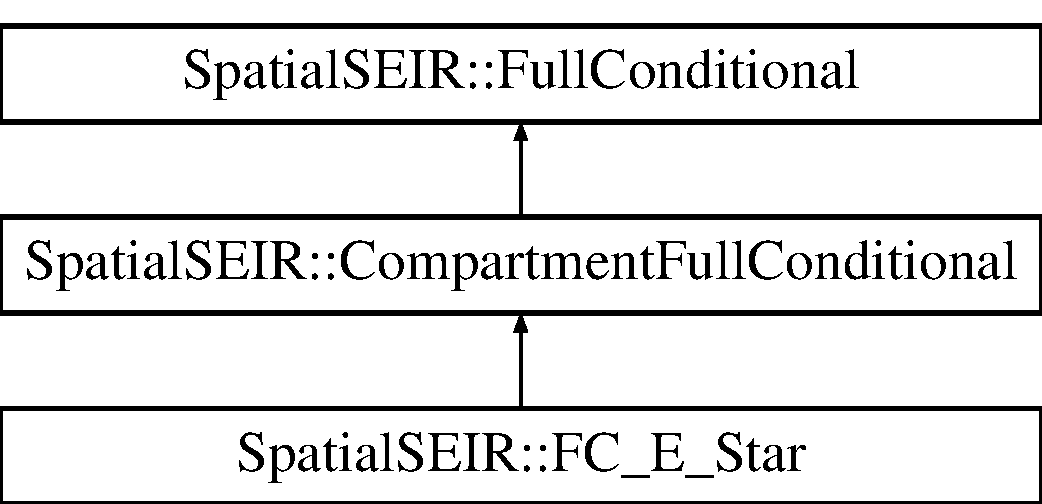
\includegraphics[height=3.000000cm]{classSpatialSEIR_1_1FC__E__Star}
\end{center}
\end{figure}
\subsection*{Public Member Functions}
\begin{DoxyCompactItemize}
\item 
\hyperlink{classSpatialSEIR_1_1FC__E__Star_a8ab5e396dcad65490e26840f8650e60d}{F\-C\-\_\-\-E\-\_\-\-Star} (\hyperlink{classSpatialSEIR_1_1ModelContext}{Model\-Context} $\ast$\-\_\-context, \hyperlink{classSpatialSEIR_1_1CompartmentalModelMatrix}{Compartmental\-Model\-Matrix} $\ast$\-\_\-\-E\-\_\-star, \hyperlink{classSpatialSEIR_1_1CompartmentalModelMatrix}{Compartmental\-Model\-Matrix} $\ast$\-\_\-\-E, \hyperlink{classSpatialSEIR_1_1CompartmentalModelMatrix}{Compartmental\-Model\-Matrix} $\ast$\-\_\-\-S, \hyperlink{classSpatialSEIR_1_1CompartmentalModelMatrix}{Compartmental\-Model\-Matrix} $\ast$\-\_\-\-I\-\_\-star, \hyperlink{classSpatialSEIR_1_1CovariateMatrix}{Covariate\-Matrix} $\ast$\-\_\-\-X, \hyperlink{classSpatialSEIR_1_1InitData}{Init\-Data} $\ast$\-\_\-\-A0, double $\ast$\-\_\-p\-\_\-se, double $\ast$\-\_\-p\-\_\-ei, double $\ast$\-\_\-rho, double $\ast$\-\_\-beta, double \-\_\-steady\-State\-Constraint\-Precision, double \hyperlink{classSpatialSEIR_1_1FullConditional_a150ee031af8d086ad0a04b13630a110f}{slice\-Width})
\item 
\hyperlink{classSpatialSEIR_1_1FC__E__Star_a98ef08bbb6df10be653ca6378df999f9}{$\sim$\-F\-C\-\_\-\-E\-\_\-\-Star} ()
\item 
virtual int \hyperlink{classSpatialSEIR_1_1FC__E__Star_aa2ab67da56b73273fa65a08dfa888edc}{eval\-C\-P\-U} ()
\item 
virtual int \hyperlink{classSpatialSEIR_1_1FC__E__Star_afd869deb206dbf7f3bc9a7666889789f}{eval\-C\-P\-U} (int i, int j)
\item 
virtual int \hyperlink{classSpatialSEIR_1_1FC__E__Star_a3e8a1e567c74935e6162b12f6f88766e}{eval\-O\-C\-L} ()
\item 
virtual void \hyperlink{classSpatialSEIR_1_1FC__E__Star_a1b3d3d4cc4b384bbe35952ac8cc884be}{sample} (int verbose)
\item 
virtual long double \hyperlink{classSpatialSEIR_1_1FC__E__Star_aa5df0a2e3cc79e4d01db7a39bab33d4f}{get\-Value} ()
\item 
virtual void \hyperlink{classSpatialSEIR_1_1FC__E__Star_a5d478a601b037cec1d430f8daa7b8cf1}{set\-Value} (long double val)
\item 
virtual int \hyperlink{classSpatialSEIR_1_1FC__E__Star_a3319916883c6d718ce6a361c6b89064e}{calculate\-Relevant\-Compartments} ()
\item 
virtual int \hyperlink{classSpatialSEIR_1_1FC__E__Star_a411225f483aa006803538599e6ee1bba}{calculate\-Relevant\-Compartments} (int i, int j)
\item 
virtual int \hyperlink{classSpatialSEIR_1_1FC__E__Star_a92265cb76c12e8527634f9b2dce07962}{calculate\-Relevant\-Compartments\-\_\-\-O\-C\-L} ()
\end{DoxyCompactItemize}
\subsection*{Public Attributes}
\begin{DoxyCompactItemize}
\item 
\hyperlink{classSpatialSEIR_1_1ModelContext}{Model\-Context} $\ast$$\ast$ \hyperlink{classSpatialSEIR_1_1FC__E__Star_ad33f047de633b3863f4aed39985b8334}{context}
\item 
\hyperlink{classSpatialSEIR_1_1CompartmentalModelMatrix}{Compartmental\-Model\-Matrix} $\ast$$\ast$ \hyperlink{classSpatialSEIR_1_1FC__E__Star_ae58ad8d1ed674c67bad9b82d9a440788}{E\-\_\-star}
\item 
\hyperlink{classSpatialSEIR_1_1CompartmentalModelMatrix}{Compartmental\-Model\-Matrix} $\ast$$\ast$ \hyperlink{classSpatialSEIR_1_1FC__E__Star_a63da3f44898801dda49332e09f6fe693}{E}
\item 
\hyperlink{classSpatialSEIR_1_1CompartmentalModelMatrix}{Compartmental\-Model\-Matrix} $\ast$$\ast$ \hyperlink{classSpatialSEIR_1_1FC__E__Star_afe0fc0e4356629d5662f72b8d01f8ac0}{S}
\item 
\hyperlink{classSpatialSEIR_1_1CompartmentalModelMatrix}{Compartmental\-Model\-Matrix} $\ast$$\ast$ \hyperlink{classSpatialSEIR_1_1FC__E__Star_ab529083fb9708dd102ac8391ba58013f}{I\-\_\-star}
\item 
\hyperlink{classSpatialSEIR_1_1CovariateMatrix}{Covariate\-Matrix} $\ast$$\ast$ \hyperlink{classSpatialSEIR_1_1FC__E__Star_adbf6bb013ffffb641ab5bf08a86543d1}{X}
\item 
\hyperlink{classSpatialSEIR_1_1InitData}{Init\-Data} $\ast$$\ast$ \hyperlink{classSpatialSEIR_1_1FC__E__Star_acc74a218a4ecb0a8df09ac2ff18c7ad9}{A0}
\item 
double $\ast$$\ast$ \hyperlink{classSpatialSEIR_1_1FC__E__Star_ae0ae48d8ad6555fd6696262081e07616}{p\-\_\-se}
\item 
double $\ast$$\ast$ \hyperlink{classSpatialSEIR_1_1FC__E__Star_aaef4ec5542c0fe3d5794571239d3b783}{p\-\_\-ei}
\item 
double $\ast$$\ast$ \hyperlink{classSpatialSEIR_1_1FC__E__Star_ab44e7a5fd2d1332a5d09358f75ddc7f5}{rho}
\item 
double $\ast$$\ast$ \hyperlink{classSpatialSEIR_1_1FC__E__Star_a941f42721f292ccf0696d890e1805301}{beta}
\item 
long double $\ast$ \hyperlink{classSpatialSEIR_1_1FC__E__Star_a7e134b73759fab72fa936f7bf0ec16cd}{value}
\item 
double $\ast$ \hyperlink{classSpatialSEIR_1_1FC__E__Star_a2ef0148996094e8ca63ef706298688b6}{steady\-State\-Constraint\-Precision}
\end{DoxyCompactItemize}


\subsection{Detailed Description}
\hyperlink{classSpatialSEIR_1_1FC__E__Star}{F\-C\-\_\-\-E\-\_\-\-Star} gives the full conditional distribution of E\-\_\-star, the transition matrix capturing individuals moving from the susceptible category to the exposed category. 

\subsection{Constructor \& Destructor Documentation}
\hypertarget{classSpatialSEIR_1_1FC__E__Star_a8ab5e396dcad65490e26840f8650e60d}{\index{Spatial\-S\-E\-I\-R\-::\-F\-C\-\_\-\-E\-\_\-\-Star@{Spatial\-S\-E\-I\-R\-::\-F\-C\-\_\-\-E\-\_\-\-Star}!F\-C\-\_\-\-E\-\_\-\-Star@{F\-C\-\_\-\-E\-\_\-\-Star}}
\index{F\-C\-\_\-\-E\-\_\-\-Star@{F\-C\-\_\-\-E\-\_\-\-Star}!SpatialSEIR::FC_E_Star@{Spatial\-S\-E\-I\-R\-::\-F\-C\-\_\-\-E\-\_\-\-Star}}
\subsubsection[{F\-C\-\_\-\-E\-\_\-\-Star}]{\setlength{\rightskip}{0pt plus 5cm}Spatial\-S\-E\-I\-R\-::\-F\-C\-\_\-\-E\-\_\-\-Star\-::\-F\-C\-\_\-\-E\-\_\-\-Star (
\begin{DoxyParamCaption}
\item[{{\bf Model\-Context} $\ast$}]{\-\_\-context, }
\item[{{\bf Compartmental\-Model\-Matrix} $\ast$}]{\-\_\-\-E\-\_\-star, }
\item[{{\bf Compartmental\-Model\-Matrix} $\ast$}]{\-\_\-\-E, }
\item[{{\bf Compartmental\-Model\-Matrix} $\ast$}]{\-\_\-\-S, }
\item[{{\bf Compartmental\-Model\-Matrix} $\ast$}]{\-\_\-\-I\-\_\-star, }
\item[{{\bf Covariate\-Matrix} $\ast$}]{\-\_\-\-X, }
\item[{{\bf Init\-Data} $\ast$}]{\-\_\-\-A0, }
\item[{double $\ast$}]{\-\_\-p\-\_\-se, }
\item[{double $\ast$}]{\-\_\-p\-\_\-ei, }
\item[{double $\ast$}]{\-\_\-rho, }
\item[{double $\ast$}]{\-\_\-beta, }
\item[{double}]{\-\_\-steady\-State\-Constraint\-Precision, }
\item[{double}]{slice\-Width}
\end{DoxyParamCaption}
)}}\label{classSpatialSEIR_1_1FC__E__Star_a8ab5e396dcad65490e26840f8650e60d}
\hypertarget{classSpatialSEIR_1_1FC__E__Star_a98ef08bbb6df10be653ca6378df999f9}{\index{Spatial\-S\-E\-I\-R\-::\-F\-C\-\_\-\-E\-\_\-\-Star@{Spatial\-S\-E\-I\-R\-::\-F\-C\-\_\-\-E\-\_\-\-Star}!$\sim$\-F\-C\-\_\-\-E\-\_\-\-Star@{$\sim$\-F\-C\-\_\-\-E\-\_\-\-Star}}
\index{$\sim$\-F\-C\-\_\-\-E\-\_\-\-Star@{$\sim$\-F\-C\-\_\-\-E\-\_\-\-Star}!SpatialSEIR::FC_E_Star@{Spatial\-S\-E\-I\-R\-::\-F\-C\-\_\-\-E\-\_\-\-Star}}
\subsubsection[{$\sim$\-F\-C\-\_\-\-E\-\_\-\-Star}]{\setlength{\rightskip}{0pt plus 5cm}Spatial\-S\-E\-I\-R\-::\-F\-C\-\_\-\-E\-\_\-\-Star\-::$\sim$\-F\-C\-\_\-\-E\-\_\-\-Star (
\begin{DoxyParamCaption}
{}
\end{DoxyParamCaption}
)}}\label{classSpatialSEIR_1_1FC__E__Star_a98ef08bbb6df10be653ca6378df999f9}


\subsection{Member Function Documentation}
\hypertarget{classSpatialSEIR_1_1FC__E__Star_a3319916883c6d718ce6a361c6b89064e}{\index{Spatial\-S\-E\-I\-R\-::\-F\-C\-\_\-\-E\-\_\-\-Star@{Spatial\-S\-E\-I\-R\-::\-F\-C\-\_\-\-E\-\_\-\-Star}!calculate\-Relevant\-Compartments@{calculate\-Relevant\-Compartments}}
\index{calculate\-Relevant\-Compartments@{calculate\-Relevant\-Compartments}!SpatialSEIR::FC_E_Star@{Spatial\-S\-E\-I\-R\-::\-F\-C\-\_\-\-E\-\_\-\-Star}}
\subsubsection[{calculate\-Relevant\-Compartments}]{\setlength{\rightskip}{0pt plus 5cm}int Spatial\-S\-E\-I\-R\-::\-F\-C\-\_\-\-E\-\_\-\-Star\-::calculate\-Relevant\-Compartments (
\begin{DoxyParamCaption}
{}
\end{DoxyParamCaption}
)\hspace{0.3cm}{\ttfamily [virtual]}}}\label{classSpatialSEIR_1_1FC__E__Star_a3319916883c6d718ce6a361c6b89064e}


Implements \hyperlink{classSpatialSEIR_1_1CompartmentFullConditional_a71836271b0997117f3b8437c2f55a986}{Spatial\-S\-E\-I\-R\-::\-Compartment\-Full\-Conditional}.

\hypertarget{classSpatialSEIR_1_1FC__E__Star_a411225f483aa006803538599e6ee1bba}{\index{Spatial\-S\-E\-I\-R\-::\-F\-C\-\_\-\-E\-\_\-\-Star@{Spatial\-S\-E\-I\-R\-::\-F\-C\-\_\-\-E\-\_\-\-Star}!calculate\-Relevant\-Compartments@{calculate\-Relevant\-Compartments}}
\index{calculate\-Relevant\-Compartments@{calculate\-Relevant\-Compartments}!SpatialSEIR::FC_E_Star@{Spatial\-S\-E\-I\-R\-::\-F\-C\-\_\-\-E\-\_\-\-Star}}
\subsubsection[{calculate\-Relevant\-Compartments}]{\setlength{\rightskip}{0pt plus 5cm}int Spatial\-S\-E\-I\-R\-::\-F\-C\-\_\-\-E\-\_\-\-Star\-::calculate\-Relevant\-Compartments (
\begin{DoxyParamCaption}
\item[{int}]{i, }
\item[{int}]{j}
\end{DoxyParamCaption}
)\hspace{0.3cm}{\ttfamily [virtual]}}}\label{classSpatialSEIR_1_1FC__E__Star_a411225f483aa006803538599e6ee1bba}


Implements \hyperlink{classSpatialSEIR_1_1CompartmentFullConditional_a21440bf07bd554a2893a328713bfe09f}{Spatial\-S\-E\-I\-R\-::\-Compartment\-Full\-Conditional}.

\hypertarget{classSpatialSEIR_1_1FC__E__Star_a92265cb76c12e8527634f9b2dce07962}{\index{Spatial\-S\-E\-I\-R\-::\-F\-C\-\_\-\-E\-\_\-\-Star@{Spatial\-S\-E\-I\-R\-::\-F\-C\-\_\-\-E\-\_\-\-Star}!calculate\-Relevant\-Compartments\-\_\-\-O\-C\-L@{calculate\-Relevant\-Compartments\-\_\-\-O\-C\-L}}
\index{calculate\-Relevant\-Compartments\-\_\-\-O\-C\-L@{calculate\-Relevant\-Compartments\-\_\-\-O\-C\-L}!SpatialSEIR::FC_E_Star@{Spatial\-S\-E\-I\-R\-::\-F\-C\-\_\-\-E\-\_\-\-Star}}
\subsubsection[{calculate\-Relevant\-Compartments\-\_\-\-O\-C\-L}]{\setlength{\rightskip}{0pt plus 5cm}int Spatial\-S\-E\-I\-R\-::\-F\-C\-\_\-\-E\-\_\-\-Star\-::calculate\-Relevant\-Compartments\-\_\-\-O\-C\-L (
\begin{DoxyParamCaption}
{}
\end{DoxyParamCaption}
)\hspace{0.3cm}{\ttfamily [virtual]}}}\label{classSpatialSEIR_1_1FC__E__Star_a92265cb76c12e8527634f9b2dce07962}


Implements \hyperlink{classSpatialSEIR_1_1CompartmentFullConditional_ab873ecc59f7639637113d885ab89bed4}{Spatial\-S\-E\-I\-R\-::\-Compartment\-Full\-Conditional}.

\hypertarget{classSpatialSEIR_1_1FC__E__Star_aa2ab67da56b73273fa65a08dfa888edc}{\index{Spatial\-S\-E\-I\-R\-::\-F\-C\-\_\-\-E\-\_\-\-Star@{Spatial\-S\-E\-I\-R\-::\-F\-C\-\_\-\-E\-\_\-\-Star}!eval\-C\-P\-U@{eval\-C\-P\-U}}
\index{eval\-C\-P\-U@{eval\-C\-P\-U}!SpatialSEIR::FC_E_Star@{Spatial\-S\-E\-I\-R\-::\-F\-C\-\_\-\-E\-\_\-\-Star}}
\subsubsection[{eval\-C\-P\-U}]{\setlength{\rightskip}{0pt plus 5cm}int Spatial\-S\-E\-I\-R\-::\-F\-C\-\_\-\-E\-\_\-\-Star\-::eval\-C\-P\-U (
\begin{DoxyParamCaption}
{}
\end{DoxyParamCaption}
)\hspace{0.3cm}{\ttfamily [virtual]}}}\label{classSpatialSEIR_1_1FC__E__Star_aa2ab67da56b73273fa65a08dfa888edc}


Implements \hyperlink{classSpatialSEIR_1_1CompartmentFullConditional_ad2402c8d7fc0b362482bcd5ceaa035af}{Spatial\-S\-E\-I\-R\-::\-Compartment\-Full\-Conditional}.

\hypertarget{classSpatialSEIR_1_1FC__E__Star_afd869deb206dbf7f3bc9a7666889789f}{\index{Spatial\-S\-E\-I\-R\-::\-F\-C\-\_\-\-E\-\_\-\-Star@{Spatial\-S\-E\-I\-R\-::\-F\-C\-\_\-\-E\-\_\-\-Star}!eval\-C\-P\-U@{eval\-C\-P\-U}}
\index{eval\-C\-P\-U@{eval\-C\-P\-U}!SpatialSEIR::FC_E_Star@{Spatial\-S\-E\-I\-R\-::\-F\-C\-\_\-\-E\-\_\-\-Star}}
\subsubsection[{eval\-C\-P\-U}]{\setlength{\rightskip}{0pt plus 5cm}int Spatial\-S\-E\-I\-R\-::\-F\-C\-\_\-\-E\-\_\-\-Star\-::eval\-C\-P\-U (
\begin{DoxyParamCaption}
\item[{int}]{i, }
\item[{int}]{j}
\end{DoxyParamCaption}
)\hspace{0.3cm}{\ttfamily [virtual]}}}\label{classSpatialSEIR_1_1FC__E__Star_afd869deb206dbf7f3bc9a7666889789f}


Implements \hyperlink{classSpatialSEIR_1_1CompartmentFullConditional_a92d48bc8cd13ff048791edbdcc453479}{Spatial\-S\-E\-I\-R\-::\-Compartment\-Full\-Conditional}.

\hypertarget{classSpatialSEIR_1_1FC__E__Star_a3e8a1e567c74935e6162b12f6f88766e}{\index{Spatial\-S\-E\-I\-R\-::\-F\-C\-\_\-\-E\-\_\-\-Star@{Spatial\-S\-E\-I\-R\-::\-F\-C\-\_\-\-E\-\_\-\-Star}!eval\-O\-C\-L@{eval\-O\-C\-L}}
\index{eval\-O\-C\-L@{eval\-O\-C\-L}!SpatialSEIR::FC_E_Star@{Spatial\-S\-E\-I\-R\-::\-F\-C\-\_\-\-E\-\_\-\-Star}}
\subsubsection[{eval\-O\-C\-L}]{\setlength{\rightskip}{0pt plus 5cm}int Spatial\-S\-E\-I\-R\-::\-F\-C\-\_\-\-E\-\_\-\-Star\-::eval\-O\-C\-L (
\begin{DoxyParamCaption}
{}
\end{DoxyParamCaption}
)\hspace{0.3cm}{\ttfamily [virtual]}}}\label{classSpatialSEIR_1_1FC__E__Star_a3e8a1e567c74935e6162b12f6f88766e}


Implements \hyperlink{classSpatialSEIR_1_1CompartmentFullConditional_ac7c7b1191508d49a56ec739449bf93d4}{Spatial\-S\-E\-I\-R\-::\-Compartment\-Full\-Conditional}.

\hypertarget{classSpatialSEIR_1_1FC__E__Star_aa5df0a2e3cc79e4d01db7a39bab33d4f}{\index{Spatial\-S\-E\-I\-R\-::\-F\-C\-\_\-\-E\-\_\-\-Star@{Spatial\-S\-E\-I\-R\-::\-F\-C\-\_\-\-E\-\_\-\-Star}!get\-Value@{get\-Value}}
\index{get\-Value@{get\-Value}!SpatialSEIR::FC_E_Star@{Spatial\-S\-E\-I\-R\-::\-F\-C\-\_\-\-E\-\_\-\-Star}}
\subsubsection[{get\-Value}]{\setlength{\rightskip}{0pt plus 5cm}long double Spatial\-S\-E\-I\-R\-::\-F\-C\-\_\-\-E\-\_\-\-Star\-::get\-Value (
\begin{DoxyParamCaption}
{}
\end{DoxyParamCaption}
)\hspace{0.3cm}{\ttfamily [virtual]}}}\label{classSpatialSEIR_1_1FC__E__Star_aa5df0a2e3cc79e4d01db7a39bab33d4f}


Implements \hyperlink{classSpatialSEIR_1_1CompartmentFullConditional_a28794be23ee7f6fcba96ff2bee63e065}{Spatial\-S\-E\-I\-R\-::\-Compartment\-Full\-Conditional}.

\hypertarget{classSpatialSEIR_1_1FC__E__Star_a1b3d3d4cc4b384bbe35952ac8cc884be}{\index{Spatial\-S\-E\-I\-R\-::\-F\-C\-\_\-\-E\-\_\-\-Star@{Spatial\-S\-E\-I\-R\-::\-F\-C\-\_\-\-E\-\_\-\-Star}!sample@{sample}}
\index{sample@{sample}!SpatialSEIR::FC_E_Star@{Spatial\-S\-E\-I\-R\-::\-F\-C\-\_\-\-E\-\_\-\-Star}}
\subsubsection[{sample}]{\setlength{\rightskip}{0pt plus 5cm}void Spatial\-S\-E\-I\-R\-::\-F\-C\-\_\-\-E\-\_\-\-Star\-::sample (
\begin{DoxyParamCaption}
\item[{int}]{verbose}
\end{DoxyParamCaption}
)\hspace{0.3cm}{\ttfamily [virtual]}}}\label{classSpatialSEIR_1_1FC__E__Star_a1b3d3d4cc4b384bbe35952ac8cc884be}


Implements \hyperlink{classSpatialSEIR_1_1CompartmentFullConditional_a436ae9e47f7a4269f0a78ce225e6b7f3}{Spatial\-S\-E\-I\-R\-::\-Compartment\-Full\-Conditional}.

\hypertarget{classSpatialSEIR_1_1FC__E__Star_a5d478a601b037cec1d430f8daa7b8cf1}{\index{Spatial\-S\-E\-I\-R\-::\-F\-C\-\_\-\-E\-\_\-\-Star@{Spatial\-S\-E\-I\-R\-::\-F\-C\-\_\-\-E\-\_\-\-Star}!set\-Value@{set\-Value}}
\index{set\-Value@{set\-Value}!SpatialSEIR::FC_E_Star@{Spatial\-S\-E\-I\-R\-::\-F\-C\-\_\-\-E\-\_\-\-Star}}
\subsubsection[{set\-Value}]{\setlength{\rightskip}{0pt plus 5cm}void Spatial\-S\-E\-I\-R\-::\-F\-C\-\_\-\-E\-\_\-\-Star\-::set\-Value (
\begin{DoxyParamCaption}
\item[{long double}]{val}
\end{DoxyParamCaption}
)\hspace{0.3cm}{\ttfamily [virtual]}}}\label{classSpatialSEIR_1_1FC__E__Star_a5d478a601b037cec1d430f8daa7b8cf1}


Implements \hyperlink{classSpatialSEIR_1_1CompartmentFullConditional_a22ab4dcc354c8ebc4f619685bc32dfae}{Spatial\-S\-E\-I\-R\-::\-Compartment\-Full\-Conditional}.



\subsection{Member Data Documentation}
\hypertarget{classSpatialSEIR_1_1FC__E__Star_acc74a218a4ecb0a8df09ac2ff18c7ad9}{\index{Spatial\-S\-E\-I\-R\-::\-F\-C\-\_\-\-E\-\_\-\-Star@{Spatial\-S\-E\-I\-R\-::\-F\-C\-\_\-\-E\-\_\-\-Star}!A0@{A0}}
\index{A0@{A0}!SpatialSEIR::FC_E_Star@{Spatial\-S\-E\-I\-R\-::\-F\-C\-\_\-\-E\-\_\-\-Star}}
\subsubsection[{A0}]{\setlength{\rightskip}{0pt plus 5cm}{\bf Init\-Data}$\ast$$\ast$ Spatial\-S\-E\-I\-R\-::\-F\-C\-\_\-\-E\-\_\-\-Star\-::\-A0}}\label{classSpatialSEIR_1_1FC__E__Star_acc74a218a4ecb0a8df09ac2ff18c7ad9}
\hypertarget{classSpatialSEIR_1_1FC__E__Star_a941f42721f292ccf0696d890e1805301}{\index{Spatial\-S\-E\-I\-R\-::\-F\-C\-\_\-\-E\-\_\-\-Star@{Spatial\-S\-E\-I\-R\-::\-F\-C\-\_\-\-E\-\_\-\-Star}!beta@{beta}}
\index{beta@{beta}!SpatialSEIR::FC_E_Star@{Spatial\-S\-E\-I\-R\-::\-F\-C\-\_\-\-E\-\_\-\-Star}}
\subsubsection[{beta}]{\setlength{\rightskip}{0pt plus 5cm}double$\ast$$\ast$ Spatial\-S\-E\-I\-R\-::\-F\-C\-\_\-\-E\-\_\-\-Star\-::beta}}\label{classSpatialSEIR_1_1FC__E__Star_a941f42721f292ccf0696d890e1805301}
\hypertarget{classSpatialSEIR_1_1FC__E__Star_ad33f047de633b3863f4aed39985b8334}{\index{Spatial\-S\-E\-I\-R\-::\-F\-C\-\_\-\-E\-\_\-\-Star@{Spatial\-S\-E\-I\-R\-::\-F\-C\-\_\-\-E\-\_\-\-Star}!context@{context}}
\index{context@{context}!SpatialSEIR::FC_E_Star@{Spatial\-S\-E\-I\-R\-::\-F\-C\-\_\-\-E\-\_\-\-Star}}
\subsubsection[{context}]{\setlength{\rightskip}{0pt plus 5cm}{\bf Model\-Context}$\ast$$\ast$ Spatial\-S\-E\-I\-R\-::\-F\-C\-\_\-\-E\-\_\-\-Star\-::context}}\label{classSpatialSEIR_1_1FC__E__Star_ad33f047de633b3863f4aed39985b8334}
\hypertarget{classSpatialSEIR_1_1FC__E__Star_a63da3f44898801dda49332e09f6fe693}{\index{Spatial\-S\-E\-I\-R\-::\-F\-C\-\_\-\-E\-\_\-\-Star@{Spatial\-S\-E\-I\-R\-::\-F\-C\-\_\-\-E\-\_\-\-Star}!E@{E}}
\index{E@{E}!SpatialSEIR::FC_E_Star@{Spatial\-S\-E\-I\-R\-::\-F\-C\-\_\-\-E\-\_\-\-Star}}
\subsubsection[{E}]{\setlength{\rightskip}{0pt plus 5cm}{\bf Compartmental\-Model\-Matrix}$\ast$$\ast$ Spatial\-S\-E\-I\-R\-::\-F\-C\-\_\-\-E\-\_\-\-Star\-::\-E}}\label{classSpatialSEIR_1_1FC__E__Star_a63da3f44898801dda49332e09f6fe693}
\hypertarget{classSpatialSEIR_1_1FC__E__Star_ae58ad8d1ed674c67bad9b82d9a440788}{\index{Spatial\-S\-E\-I\-R\-::\-F\-C\-\_\-\-E\-\_\-\-Star@{Spatial\-S\-E\-I\-R\-::\-F\-C\-\_\-\-E\-\_\-\-Star}!E\-\_\-star@{E\-\_\-star}}
\index{E\-\_\-star@{E\-\_\-star}!SpatialSEIR::FC_E_Star@{Spatial\-S\-E\-I\-R\-::\-F\-C\-\_\-\-E\-\_\-\-Star}}
\subsubsection[{E\-\_\-star}]{\setlength{\rightskip}{0pt plus 5cm}{\bf Compartmental\-Model\-Matrix}$\ast$$\ast$ Spatial\-S\-E\-I\-R\-::\-F\-C\-\_\-\-E\-\_\-\-Star\-::\-E\-\_\-star}}\label{classSpatialSEIR_1_1FC__E__Star_ae58ad8d1ed674c67bad9b82d9a440788}
\hypertarget{classSpatialSEIR_1_1FC__E__Star_ab529083fb9708dd102ac8391ba58013f}{\index{Spatial\-S\-E\-I\-R\-::\-F\-C\-\_\-\-E\-\_\-\-Star@{Spatial\-S\-E\-I\-R\-::\-F\-C\-\_\-\-E\-\_\-\-Star}!I\-\_\-star@{I\-\_\-star}}
\index{I\-\_\-star@{I\-\_\-star}!SpatialSEIR::FC_E_Star@{Spatial\-S\-E\-I\-R\-::\-F\-C\-\_\-\-E\-\_\-\-Star}}
\subsubsection[{I\-\_\-star}]{\setlength{\rightskip}{0pt plus 5cm}{\bf Compartmental\-Model\-Matrix}$\ast$$\ast$ Spatial\-S\-E\-I\-R\-::\-F\-C\-\_\-\-E\-\_\-\-Star\-::\-I\-\_\-star}}\label{classSpatialSEIR_1_1FC__E__Star_ab529083fb9708dd102ac8391ba58013f}
\hypertarget{classSpatialSEIR_1_1FC__E__Star_aaef4ec5542c0fe3d5794571239d3b783}{\index{Spatial\-S\-E\-I\-R\-::\-F\-C\-\_\-\-E\-\_\-\-Star@{Spatial\-S\-E\-I\-R\-::\-F\-C\-\_\-\-E\-\_\-\-Star}!p\-\_\-ei@{p\-\_\-ei}}
\index{p\-\_\-ei@{p\-\_\-ei}!SpatialSEIR::FC_E_Star@{Spatial\-S\-E\-I\-R\-::\-F\-C\-\_\-\-E\-\_\-\-Star}}
\subsubsection[{p\-\_\-ei}]{\setlength{\rightskip}{0pt plus 5cm}double$\ast$$\ast$ Spatial\-S\-E\-I\-R\-::\-F\-C\-\_\-\-E\-\_\-\-Star\-::p\-\_\-ei}}\label{classSpatialSEIR_1_1FC__E__Star_aaef4ec5542c0fe3d5794571239d3b783}
\hypertarget{classSpatialSEIR_1_1FC__E__Star_ae0ae48d8ad6555fd6696262081e07616}{\index{Spatial\-S\-E\-I\-R\-::\-F\-C\-\_\-\-E\-\_\-\-Star@{Spatial\-S\-E\-I\-R\-::\-F\-C\-\_\-\-E\-\_\-\-Star}!p\-\_\-se@{p\-\_\-se}}
\index{p\-\_\-se@{p\-\_\-se}!SpatialSEIR::FC_E_Star@{Spatial\-S\-E\-I\-R\-::\-F\-C\-\_\-\-E\-\_\-\-Star}}
\subsubsection[{p\-\_\-se}]{\setlength{\rightskip}{0pt plus 5cm}double$\ast$$\ast$ Spatial\-S\-E\-I\-R\-::\-F\-C\-\_\-\-E\-\_\-\-Star\-::p\-\_\-se}}\label{classSpatialSEIR_1_1FC__E__Star_ae0ae48d8ad6555fd6696262081e07616}
\hypertarget{classSpatialSEIR_1_1FC__E__Star_ab44e7a5fd2d1332a5d09358f75ddc7f5}{\index{Spatial\-S\-E\-I\-R\-::\-F\-C\-\_\-\-E\-\_\-\-Star@{Spatial\-S\-E\-I\-R\-::\-F\-C\-\_\-\-E\-\_\-\-Star}!rho@{rho}}
\index{rho@{rho}!SpatialSEIR::FC_E_Star@{Spatial\-S\-E\-I\-R\-::\-F\-C\-\_\-\-E\-\_\-\-Star}}
\subsubsection[{rho}]{\setlength{\rightskip}{0pt plus 5cm}double$\ast$$\ast$ Spatial\-S\-E\-I\-R\-::\-F\-C\-\_\-\-E\-\_\-\-Star\-::rho}}\label{classSpatialSEIR_1_1FC__E__Star_ab44e7a5fd2d1332a5d09358f75ddc7f5}
\hypertarget{classSpatialSEIR_1_1FC__E__Star_afe0fc0e4356629d5662f72b8d01f8ac0}{\index{Spatial\-S\-E\-I\-R\-::\-F\-C\-\_\-\-E\-\_\-\-Star@{Spatial\-S\-E\-I\-R\-::\-F\-C\-\_\-\-E\-\_\-\-Star}!S@{S}}
\index{S@{S}!SpatialSEIR::FC_E_Star@{Spatial\-S\-E\-I\-R\-::\-F\-C\-\_\-\-E\-\_\-\-Star}}
\subsubsection[{S}]{\setlength{\rightskip}{0pt plus 5cm}{\bf Compartmental\-Model\-Matrix}$\ast$$\ast$ Spatial\-S\-E\-I\-R\-::\-F\-C\-\_\-\-E\-\_\-\-Star\-::\-S}}\label{classSpatialSEIR_1_1FC__E__Star_afe0fc0e4356629d5662f72b8d01f8ac0}
\hypertarget{classSpatialSEIR_1_1FC__E__Star_a2ef0148996094e8ca63ef706298688b6}{\index{Spatial\-S\-E\-I\-R\-::\-F\-C\-\_\-\-E\-\_\-\-Star@{Spatial\-S\-E\-I\-R\-::\-F\-C\-\_\-\-E\-\_\-\-Star}!steady\-State\-Constraint\-Precision@{steady\-State\-Constraint\-Precision}}
\index{steady\-State\-Constraint\-Precision@{steady\-State\-Constraint\-Precision}!SpatialSEIR::FC_E_Star@{Spatial\-S\-E\-I\-R\-::\-F\-C\-\_\-\-E\-\_\-\-Star}}
\subsubsection[{steady\-State\-Constraint\-Precision}]{\setlength{\rightskip}{0pt plus 5cm}double$\ast$ Spatial\-S\-E\-I\-R\-::\-F\-C\-\_\-\-E\-\_\-\-Star\-::steady\-State\-Constraint\-Precision}}\label{classSpatialSEIR_1_1FC__E__Star_a2ef0148996094e8ca63ef706298688b6}
\hypertarget{classSpatialSEIR_1_1FC__E__Star_a7e134b73759fab72fa936f7bf0ec16cd}{\index{Spatial\-S\-E\-I\-R\-::\-F\-C\-\_\-\-E\-\_\-\-Star@{Spatial\-S\-E\-I\-R\-::\-F\-C\-\_\-\-E\-\_\-\-Star}!value@{value}}
\index{value@{value}!SpatialSEIR::FC_E_Star@{Spatial\-S\-E\-I\-R\-::\-F\-C\-\_\-\-E\-\_\-\-Star}}
\subsubsection[{value}]{\setlength{\rightskip}{0pt plus 5cm}long double$\ast$ Spatial\-S\-E\-I\-R\-::\-F\-C\-\_\-\-E\-\_\-\-Star\-::value}}\label{classSpatialSEIR_1_1FC__E__Star_a7e134b73759fab72fa936f7bf0ec16cd}
\hypertarget{classSpatialSEIR_1_1FC__E__Star_adbf6bb013ffffb641ab5bf08a86543d1}{\index{Spatial\-S\-E\-I\-R\-::\-F\-C\-\_\-\-E\-\_\-\-Star@{Spatial\-S\-E\-I\-R\-::\-F\-C\-\_\-\-E\-\_\-\-Star}!X@{X}}
\index{X@{X}!SpatialSEIR::FC_E_Star@{Spatial\-S\-E\-I\-R\-::\-F\-C\-\_\-\-E\-\_\-\-Star}}
\subsubsection[{X}]{\setlength{\rightskip}{0pt plus 5cm}{\bf Covariate\-Matrix}$\ast$$\ast$ Spatial\-S\-E\-I\-R\-::\-F\-C\-\_\-\-E\-\_\-\-Star\-::\-X}}\label{classSpatialSEIR_1_1FC__E__Star_adbf6bb013ffffb641ab5bf08a86543d1}


The documentation for this class was generated from the following files\-:\begin{DoxyCompactItemize}
\item 
lib\-Spatial\-S\-E\-I\-R/include/\-Full\-Conditionals/\hyperlink{LSS__FC__E__star_8hpp}{L\-S\-S\-\_\-\-F\-C\-\_\-\-E\-\_\-star.\-hpp}\item 
lib\-Spatial\-S\-E\-I\-R/src/\-Full\-Conditionals/\hyperlink{FC__E__star_8cpp}{F\-C\-\_\-\-E\-\_\-star.\-cpp}\end{DoxyCompactItemize}

\hypertarget{classSpatialSEIR_1_1FC__Gamma__EI}{\section{Spatial\-S\-E\-I\-R\-:\-:F\-C\-\_\-\-Gamma\-\_\-\-E\-I Class Reference}
\label{classSpatialSEIR_1_1FC__Gamma__EI}\index{Spatial\-S\-E\-I\-R\-::\-F\-C\-\_\-\-Gamma\-\_\-\-E\-I@{Spatial\-S\-E\-I\-R\-::\-F\-C\-\_\-\-Gamma\-\_\-\-E\-I}}
}


{\ttfamily \#include $<$L\-S\-S\-\_\-\-F\-C\-\_\-\-Gamma\-\_\-\-E\-I.\-hpp$>$}

Inheritance diagram for Spatial\-S\-E\-I\-R\-:\-:F\-C\-\_\-\-Gamma\-\_\-\-E\-I\-:\begin{figure}[H]
\begin{center}
\leavevmode
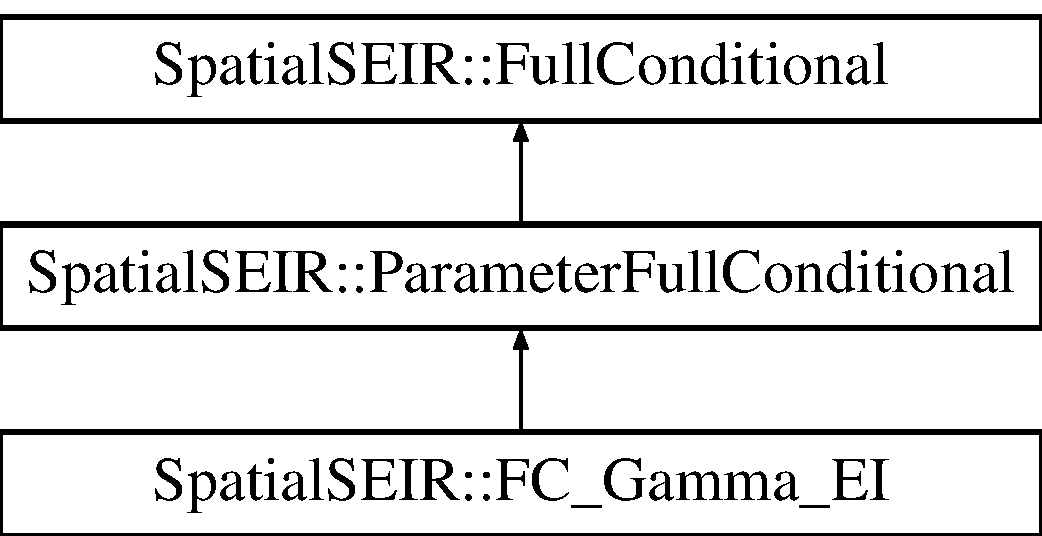
\includegraphics[height=3.000000cm]{classSpatialSEIR_1_1FC__Gamma__EI}
\end{center}
\end{figure}
\subsection*{Public Member Functions}
\begin{DoxyCompactItemize}
\item 
\hyperlink{classSpatialSEIR_1_1FC__Gamma__EI_a6d22d782fa070915060842101380c2af}{F\-C\-\_\-\-Gamma\-\_\-\-E\-I} (\hyperlink{classSpatialSEIR_1_1ModelContext}{Model\-Context} $\ast$\-\_\-context, \hyperlink{classSpatialSEIR_1_1CompartmentalModelMatrix}{Compartmental\-Model\-Matrix} $\ast$\-\_\-\-I\-\_\-star, \hyperlink{classSpatialSEIR_1_1CompartmentalModelMatrix}{Compartmental\-Model\-Matrix} $\ast$\-\_\-\-E, \hyperlink{classSpatialSEIR_1_1InitData}{Init\-Data} $\ast$\-\_\-\-A0, double $\ast$\-\_\-p\-\_\-ei, double $\ast$\-\_\-gamma\-\_\-ei, double \-\_\-prior\-Alpha, double \-\_\-prior\-Beta, double \hyperlink{classSpatialSEIR_1_1FullConditional_a150ee031af8d086ad0a04b13630a110f}{slice\-Width})
\item 
virtual double \hyperlink{classSpatialSEIR_1_1FC__Gamma__EI_a001e6dacce9fc05d2db7217349f0f31f}{eval\-Prior} ()
\item 
virtual int \hyperlink{classSpatialSEIR_1_1FC__Gamma__EI_ad04e240632b08359ae6d924d6d88fdde}{eval\-C\-P\-U} ()
\item 
virtual int \hyperlink{classSpatialSEIR_1_1FC__Gamma__EI_a30bbe6436e31914a36042488bd0ecd29}{eval\-O\-C\-L} ()
\item 
virtual void \hyperlink{classSpatialSEIR_1_1FC__Gamma__EI_a33e0d2d52a85669f64fe058292ece1f8}{sample} (int verbose)
\item 
virtual long double \hyperlink{classSpatialSEIR_1_1FC__Gamma__EI_ad33d614b75ea81d0a34eecbcec2fd406}{get\-Value} ()
\item 
virtual void \hyperlink{classSpatialSEIR_1_1FC__Gamma__EI_af1593c1841cea3c44e69d35af9640304}{set\-Value} (long double val)
\item 
virtual int \hyperlink{classSpatialSEIR_1_1FC__Gamma__EI_ab2ac7a466661c568cf20ba89bced4ac2}{calculate\-Relevant\-Compartments} ()
\item 
virtual int \hyperlink{classSpatialSEIR_1_1FC__Gamma__EI_a1a10b7a7b3f0aa18af9bc60dcf17c150}{calculate\-Relevant\-Compartments\-\_\-\-O\-C\-L} ()
\item 
\hyperlink{classSpatialSEIR_1_1FC__Gamma__EI_ac6795a381b58c3feb9b82a190bfd6b5a}{$\sim$\-F\-C\-\_\-\-Gamma\-\_\-\-E\-I} ()
\end{DoxyCompactItemize}
\subsection*{Public Attributes}
\begin{DoxyCompactItemize}
\item 
\hyperlink{classSpatialSEIR_1_1ModelContext}{Model\-Context} $\ast$$\ast$ \hyperlink{classSpatialSEIR_1_1FC__Gamma__EI_a72fcb8c17cc8abf66d56f8282397a0b2}{context}
\item 
\hyperlink{classSpatialSEIR_1_1CompartmentalModelMatrix}{Compartmental\-Model\-Matrix} $\ast$$\ast$ \hyperlink{classSpatialSEIR_1_1FC__Gamma__EI_a1160b335f074316d5c7cda9ed37c6718}{I\-\_\-star}
\item 
\hyperlink{classSpatialSEIR_1_1CompartmentalModelMatrix}{Compartmental\-Model\-Matrix} $\ast$$\ast$ \hyperlink{classSpatialSEIR_1_1FC__Gamma__EI_a0713816be274377c626114b530924f55}{E}
\item 
\hyperlink{classSpatialSEIR_1_1InitData}{Init\-Data} $\ast$$\ast$ \hyperlink{classSpatialSEIR_1_1FC__Gamma__EI_a10bf326741fabf11d4fbc734ab933049}{A0}
\item 
double $\ast$$\ast$ \hyperlink{classSpatialSEIR_1_1FC__Gamma__EI_a2d06cf55d4efdc31b421be96583cd9e7}{p\-\_\-ei}
\item 
double $\ast$$\ast$ \hyperlink{classSpatialSEIR_1_1FC__Gamma__EI_a6c9eaf49e5c3464a819cc3ed15b58001}{gamma\-\_\-ei}
\item 
long double $\ast$ \hyperlink{classSpatialSEIR_1_1FC__Gamma__EI_a925437301fd547a6cc95dbe62d061e34}{value}
\item 
double $\ast$ \hyperlink{classSpatialSEIR_1_1FC__Gamma__EI_aad60d0e3253e705c661a083889c5390e}{prior\-Alpha}
\item 
double $\ast$ \hyperlink{classSpatialSEIR_1_1FC__Gamma__EI_a784d43fdd90ee401dc597c6aae2ce952}{prior\-Beta}
\end{DoxyCompactItemize}


\subsection{Detailed Description}
\hyperlink{classSpatialSEIR_1_1FC__Gamma__EI}{F\-C\-\_\-\-Gamma\-\_\-\-E\-I} gives the full conditional distribution of gamma\-\_\-ei, the parameter driving the probability that an exposed individual becomes infectious at a given time point, p\-\_\-ei. 

\subsection{Constructor \& Destructor Documentation}
\hypertarget{classSpatialSEIR_1_1FC__Gamma__EI_a6d22d782fa070915060842101380c2af}{\index{Spatial\-S\-E\-I\-R\-::\-F\-C\-\_\-\-Gamma\-\_\-\-E\-I@{Spatial\-S\-E\-I\-R\-::\-F\-C\-\_\-\-Gamma\-\_\-\-E\-I}!F\-C\-\_\-\-Gamma\-\_\-\-E\-I@{F\-C\-\_\-\-Gamma\-\_\-\-E\-I}}
\index{F\-C\-\_\-\-Gamma\-\_\-\-E\-I@{F\-C\-\_\-\-Gamma\-\_\-\-E\-I}!SpatialSEIR::FC_Gamma_EI@{Spatial\-S\-E\-I\-R\-::\-F\-C\-\_\-\-Gamma\-\_\-\-E\-I}}
\subsubsection[{F\-C\-\_\-\-Gamma\-\_\-\-E\-I}]{\setlength{\rightskip}{0pt plus 5cm}Spatial\-S\-E\-I\-R\-::\-F\-C\-\_\-\-Gamma\-\_\-\-E\-I\-::\-F\-C\-\_\-\-Gamma\-\_\-\-E\-I (
\begin{DoxyParamCaption}
\item[{{\bf Model\-Context} $\ast$}]{\-\_\-context, }
\item[{{\bf Compartmental\-Model\-Matrix} $\ast$}]{\-\_\-\-I\-\_\-star, }
\item[{{\bf Compartmental\-Model\-Matrix} $\ast$}]{\-\_\-\-E, }
\item[{{\bf Init\-Data} $\ast$}]{\-\_\-\-A0, }
\item[{double $\ast$}]{\-\_\-p\-\_\-ei, }
\item[{double $\ast$}]{\-\_\-gamma\-\_\-ei, }
\item[{double}]{\-\_\-prior\-Alpha, }
\item[{double}]{\-\_\-prior\-Beta, }
\item[{double}]{slice\-Width}
\end{DoxyParamCaption}
)}}\label{classSpatialSEIR_1_1FC__Gamma__EI_a6d22d782fa070915060842101380c2af}
\hypertarget{classSpatialSEIR_1_1FC__Gamma__EI_ac6795a381b58c3feb9b82a190bfd6b5a}{\index{Spatial\-S\-E\-I\-R\-::\-F\-C\-\_\-\-Gamma\-\_\-\-E\-I@{Spatial\-S\-E\-I\-R\-::\-F\-C\-\_\-\-Gamma\-\_\-\-E\-I}!$\sim$\-F\-C\-\_\-\-Gamma\-\_\-\-E\-I@{$\sim$\-F\-C\-\_\-\-Gamma\-\_\-\-E\-I}}
\index{$\sim$\-F\-C\-\_\-\-Gamma\-\_\-\-E\-I@{$\sim$\-F\-C\-\_\-\-Gamma\-\_\-\-E\-I}!SpatialSEIR::FC_Gamma_EI@{Spatial\-S\-E\-I\-R\-::\-F\-C\-\_\-\-Gamma\-\_\-\-E\-I}}
\subsubsection[{$\sim$\-F\-C\-\_\-\-Gamma\-\_\-\-E\-I}]{\setlength{\rightskip}{0pt plus 5cm}Spatial\-S\-E\-I\-R\-::\-F\-C\-\_\-\-Gamma\-\_\-\-E\-I\-::$\sim$\-F\-C\-\_\-\-Gamma\-\_\-\-E\-I (
\begin{DoxyParamCaption}
{}
\end{DoxyParamCaption}
)}}\label{classSpatialSEIR_1_1FC__Gamma__EI_ac6795a381b58c3feb9b82a190bfd6b5a}


\subsection{Member Function Documentation}
\hypertarget{classSpatialSEIR_1_1FC__Gamma__EI_ab2ac7a466661c568cf20ba89bced4ac2}{\index{Spatial\-S\-E\-I\-R\-::\-F\-C\-\_\-\-Gamma\-\_\-\-E\-I@{Spatial\-S\-E\-I\-R\-::\-F\-C\-\_\-\-Gamma\-\_\-\-E\-I}!calculate\-Relevant\-Compartments@{calculate\-Relevant\-Compartments}}
\index{calculate\-Relevant\-Compartments@{calculate\-Relevant\-Compartments}!SpatialSEIR::FC_Gamma_EI@{Spatial\-S\-E\-I\-R\-::\-F\-C\-\_\-\-Gamma\-\_\-\-E\-I}}
\subsubsection[{calculate\-Relevant\-Compartments}]{\setlength{\rightskip}{0pt plus 5cm}int Spatial\-S\-E\-I\-R\-::\-F\-C\-\_\-\-Gamma\-\_\-\-E\-I\-::calculate\-Relevant\-Compartments (
\begin{DoxyParamCaption}
{}
\end{DoxyParamCaption}
)\hspace{0.3cm}{\ttfamily [virtual]}}}\label{classSpatialSEIR_1_1FC__Gamma__EI_ab2ac7a466661c568cf20ba89bced4ac2}


Implements \hyperlink{classSpatialSEIR_1_1ParameterFullConditional_a65c39a2c3ca56e2f194b78cd362d35f9}{Spatial\-S\-E\-I\-R\-::\-Parameter\-Full\-Conditional}.

\hypertarget{classSpatialSEIR_1_1FC__Gamma__EI_a1a10b7a7b3f0aa18af9bc60dcf17c150}{\index{Spatial\-S\-E\-I\-R\-::\-F\-C\-\_\-\-Gamma\-\_\-\-E\-I@{Spatial\-S\-E\-I\-R\-::\-F\-C\-\_\-\-Gamma\-\_\-\-E\-I}!calculate\-Relevant\-Compartments\-\_\-\-O\-C\-L@{calculate\-Relevant\-Compartments\-\_\-\-O\-C\-L}}
\index{calculate\-Relevant\-Compartments\-\_\-\-O\-C\-L@{calculate\-Relevant\-Compartments\-\_\-\-O\-C\-L}!SpatialSEIR::FC_Gamma_EI@{Spatial\-S\-E\-I\-R\-::\-F\-C\-\_\-\-Gamma\-\_\-\-E\-I}}
\subsubsection[{calculate\-Relevant\-Compartments\-\_\-\-O\-C\-L}]{\setlength{\rightskip}{0pt plus 5cm}int Spatial\-S\-E\-I\-R\-::\-F\-C\-\_\-\-Gamma\-\_\-\-E\-I\-::calculate\-Relevant\-Compartments\-\_\-\-O\-C\-L (
\begin{DoxyParamCaption}
{}
\end{DoxyParamCaption}
)\hspace{0.3cm}{\ttfamily [virtual]}}}\label{classSpatialSEIR_1_1FC__Gamma__EI_a1a10b7a7b3f0aa18af9bc60dcf17c150}


Implements \hyperlink{classSpatialSEIR_1_1ParameterFullConditional_af40754537736a64f58848e0368b001fb}{Spatial\-S\-E\-I\-R\-::\-Parameter\-Full\-Conditional}.

\hypertarget{classSpatialSEIR_1_1FC__Gamma__EI_ad04e240632b08359ae6d924d6d88fdde}{\index{Spatial\-S\-E\-I\-R\-::\-F\-C\-\_\-\-Gamma\-\_\-\-E\-I@{Spatial\-S\-E\-I\-R\-::\-F\-C\-\_\-\-Gamma\-\_\-\-E\-I}!eval\-C\-P\-U@{eval\-C\-P\-U}}
\index{eval\-C\-P\-U@{eval\-C\-P\-U}!SpatialSEIR::FC_Gamma_EI@{Spatial\-S\-E\-I\-R\-::\-F\-C\-\_\-\-Gamma\-\_\-\-E\-I}}
\subsubsection[{eval\-C\-P\-U}]{\setlength{\rightskip}{0pt plus 5cm}int Spatial\-S\-E\-I\-R\-::\-F\-C\-\_\-\-Gamma\-\_\-\-E\-I\-::eval\-C\-P\-U (
\begin{DoxyParamCaption}
{}
\end{DoxyParamCaption}
)\hspace{0.3cm}{\ttfamily [virtual]}}}\label{classSpatialSEIR_1_1FC__Gamma__EI_ad04e240632b08359ae6d924d6d88fdde}


Implements \hyperlink{classSpatialSEIR_1_1ParameterFullConditional_a186bd19fdeb52ca4522f56fb880201dd}{Spatial\-S\-E\-I\-R\-::\-Parameter\-Full\-Conditional}.

\hypertarget{classSpatialSEIR_1_1FC__Gamma__EI_a30bbe6436e31914a36042488bd0ecd29}{\index{Spatial\-S\-E\-I\-R\-::\-F\-C\-\_\-\-Gamma\-\_\-\-E\-I@{Spatial\-S\-E\-I\-R\-::\-F\-C\-\_\-\-Gamma\-\_\-\-E\-I}!eval\-O\-C\-L@{eval\-O\-C\-L}}
\index{eval\-O\-C\-L@{eval\-O\-C\-L}!SpatialSEIR::FC_Gamma_EI@{Spatial\-S\-E\-I\-R\-::\-F\-C\-\_\-\-Gamma\-\_\-\-E\-I}}
\subsubsection[{eval\-O\-C\-L}]{\setlength{\rightskip}{0pt plus 5cm}int Spatial\-S\-E\-I\-R\-::\-F\-C\-\_\-\-Gamma\-\_\-\-E\-I\-::eval\-O\-C\-L (
\begin{DoxyParamCaption}
{}
\end{DoxyParamCaption}
)\hspace{0.3cm}{\ttfamily [virtual]}}}\label{classSpatialSEIR_1_1FC__Gamma__EI_a30bbe6436e31914a36042488bd0ecd29}


Implements \hyperlink{classSpatialSEIR_1_1ParameterFullConditional_ac4cfb13dace7f72e8136c45d9e959eec}{Spatial\-S\-E\-I\-R\-::\-Parameter\-Full\-Conditional}.

\hypertarget{classSpatialSEIR_1_1FC__Gamma__EI_a001e6dacce9fc05d2db7217349f0f31f}{\index{Spatial\-S\-E\-I\-R\-::\-F\-C\-\_\-\-Gamma\-\_\-\-E\-I@{Spatial\-S\-E\-I\-R\-::\-F\-C\-\_\-\-Gamma\-\_\-\-E\-I}!eval\-Prior@{eval\-Prior}}
\index{eval\-Prior@{eval\-Prior}!SpatialSEIR::FC_Gamma_EI@{Spatial\-S\-E\-I\-R\-::\-F\-C\-\_\-\-Gamma\-\_\-\-E\-I}}
\subsubsection[{eval\-Prior}]{\setlength{\rightskip}{0pt plus 5cm}double Spatial\-S\-E\-I\-R\-::\-F\-C\-\_\-\-Gamma\-\_\-\-E\-I\-::eval\-Prior (
\begin{DoxyParamCaption}
{}
\end{DoxyParamCaption}
)\hspace{0.3cm}{\ttfamily [virtual]}}}\label{classSpatialSEIR_1_1FC__Gamma__EI_a001e6dacce9fc05d2db7217349f0f31f}
\hypertarget{classSpatialSEIR_1_1FC__Gamma__EI_ad33d614b75ea81d0a34eecbcec2fd406}{\index{Spatial\-S\-E\-I\-R\-::\-F\-C\-\_\-\-Gamma\-\_\-\-E\-I@{Spatial\-S\-E\-I\-R\-::\-F\-C\-\_\-\-Gamma\-\_\-\-E\-I}!get\-Value@{get\-Value}}
\index{get\-Value@{get\-Value}!SpatialSEIR::FC_Gamma_EI@{Spatial\-S\-E\-I\-R\-::\-F\-C\-\_\-\-Gamma\-\_\-\-E\-I}}
\subsubsection[{get\-Value}]{\setlength{\rightskip}{0pt plus 5cm}long double Spatial\-S\-E\-I\-R\-::\-F\-C\-\_\-\-Gamma\-\_\-\-E\-I\-::get\-Value (
\begin{DoxyParamCaption}
{}
\end{DoxyParamCaption}
)\hspace{0.3cm}{\ttfamily [virtual]}}}\label{classSpatialSEIR_1_1FC__Gamma__EI_ad33d614b75ea81d0a34eecbcec2fd406}


Implements \hyperlink{classSpatialSEIR_1_1ParameterFullConditional_a901368d385809e77179b9fa7532adfec}{Spatial\-S\-E\-I\-R\-::\-Parameter\-Full\-Conditional}.

\hypertarget{classSpatialSEIR_1_1FC__Gamma__EI_a33e0d2d52a85669f64fe058292ece1f8}{\index{Spatial\-S\-E\-I\-R\-::\-F\-C\-\_\-\-Gamma\-\_\-\-E\-I@{Spatial\-S\-E\-I\-R\-::\-F\-C\-\_\-\-Gamma\-\_\-\-E\-I}!sample@{sample}}
\index{sample@{sample}!SpatialSEIR::FC_Gamma_EI@{Spatial\-S\-E\-I\-R\-::\-F\-C\-\_\-\-Gamma\-\_\-\-E\-I}}
\subsubsection[{sample}]{\setlength{\rightskip}{0pt plus 5cm}void Spatial\-S\-E\-I\-R\-::\-F\-C\-\_\-\-Gamma\-\_\-\-E\-I\-::sample (
\begin{DoxyParamCaption}
\item[{int}]{verbose}
\end{DoxyParamCaption}
)\hspace{0.3cm}{\ttfamily [virtual]}}}\label{classSpatialSEIR_1_1FC__Gamma__EI_a33e0d2d52a85669f64fe058292ece1f8}


Implements \hyperlink{classSpatialSEIR_1_1ParameterFullConditional_a651e22b15782acb6bd80be12bd476693}{Spatial\-S\-E\-I\-R\-::\-Parameter\-Full\-Conditional}.

\hypertarget{classSpatialSEIR_1_1FC__Gamma__EI_af1593c1841cea3c44e69d35af9640304}{\index{Spatial\-S\-E\-I\-R\-::\-F\-C\-\_\-\-Gamma\-\_\-\-E\-I@{Spatial\-S\-E\-I\-R\-::\-F\-C\-\_\-\-Gamma\-\_\-\-E\-I}!set\-Value@{set\-Value}}
\index{set\-Value@{set\-Value}!SpatialSEIR::FC_Gamma_EI@{Spatial\-S\-E\-I\-R\-::\-F\-C\-\_\-\-Gamma\-\_\-\-E\-I}}
\subsubsection[{set\-Value}]{\setlength{\rightskip}{0pt plus 5cm}void Spatial\-S\-E\-I\-R\-::\-F\-C\-\_\-\-Gamma\-\_\-\-E\-I\-::set\-Value (
\begin{DoxyParamCaption}
\item[{long double}]{val}
\end{DoxyParamCaption}
)\hspace{0.3cm}{\ttfamily [virtual]}}}\label{classSpatialSEIR_1_1FC__Gamma__EI_af1593c1841cea3c44e69d35af9640304}


Implements \hyperlink{classSpatialSEIR_1_1ParameterFullConditional_adf03f213e27d26f120b574d6dd86ffc3}{Spatial\-S\-E\-I\-R\-::\-Parameter\-Full\-Conditional}.



\subsection{Member Data Documentation}
\hypertarget{classSpatialSEIR_1_1FC__Gamma__EI_a10bf326741fabf11d4fbc734ab933049}{\index{Spatial\-S\-E\-I\-R\-::\-F\-C\-\_\-\-Gamma\-\_\-\-E\-I@{Spatial\-S\-E\-I\-R\-::\-F\-C\-\_\-\-Gamma\-\_\-\-E\-I}!A0@{A0}}
\index{A0@{A0}!SpatialSEIR::FC_Gamma_EI@{Spatial\-S\-E\-I\-R\-::\-F\-C\-\_\-\-Gamma\-\_\-\-E\-I}}
\subsubsection[{A0}]{\setlength{\rightskip}{0pt plus 5cm}{\bf Init\-Data}$\ast$$\ast$ Spatial\-S\-E\-I\-R\-::\-F\-C\-\_\-\-Gamma\-\_\-\-E\-I\-::\-A0}}\label{classSpatialSEIR_1_1FC__Gamma__EI_a10bf326741fabf11d4fbc734ab933049}
\hypertarget{classSpatialSEIR_1_1FC__Gamma__EI_a72fcb8c17cc8abf66d56f8282397a0b2}{\index{Spatial\-S\-E\-I\-R\-::\-F\-C\-\_\-\-Gamma\-\_\-\-E\-I@{Spatial\-S\-E\-I\-R\-::\-F\-C\-\_\-\-Gamma\-\_\-\-E\-I}!context@{context}}
\index{context@{context}!SpatialSEIR::FC_Gamma_EI@{Spatial\-S\-E\-I\-R\-::\-F\-C\-\_\-\-Gamma\-\_\-\-E\-I}}
\subsubsection[{context}]{\setlength{\rightskip}{0pt plus 5cm}{\bf Model\-Context}$\ast$$\ast$ Spatial\-S\-E\-I\-R\-::\-F\-C\-\_\-\-Gamma\-\_\-\-E\-I\-::context}}\label{classSpatialSEIR_1_1FC__Gamma__EI_a72fcb8c17cc8abf66d56f8282397a0b2}
\hypertarget{classSpatialSEIR_1_1FC__Gamma__EI_a0713816be274377c626114b530924f55}{\index{Spatial\-S\-E\-I\-R\-::\-F\-C\-\_\-\-Gamma\-\_\-\-E\-I@{Spatial\-S\-E\-I\-R\-::\-F\-C\-\_\-\-Gamma\-\_\-\-E\-I}!E@{E}}
\index{E@{E}!SpatialSEIR::FC_Gamma_EI@{Spatial\-S\-E\-I\-R\-::\-F\-C\-\_\-\-Gamma\-\_\-\-E\-I}}
\subsubsection[{E}]{\setlength{\rightskip}{0pt plus 5cm}{\bf Compartmental\-Model\-Matrix}$\ast$$\ast$ Spatial\-S\-E\-I\-R\-::\-F\-C\-\_\-\-Gamma\-\_\-\-E\-I\-::\-E}}\label{classSpatialSEIR_1_1FC__Gamma__EI_a0713816be274377c626114b530924f55}
\hypertarget{classSpatialSEIR_1_1FC__Gamma__EI_a6c9eaf49e5c3464a819cc3ed15b58001}{\index{Spatial\-S\-E\-I\-R\-::\-F\-C\-\_\-\-Gamma\-\_\-\-E\-I@{Spatial\-S\-E\-I\-R\-::\-F\-C\-\_\-\-Gamma\-\_\-\-E\-I}!gamma\-\_\-ei@{gamma\-\_\-ei}}
\index{gamma\-\_\-ei@{gamma\-\_\-ei}!SpatialSEIR::FC_Gamma_EI@{Spatial\-S\-E\-I\-R\-::\-F\-C\-\_\-\-Gamma\-\_\-\-E\-I}}
\subsubsection[{gamma\-\_\-ei}]{\setlength{\rightskip}{0pt plus 5cm}double$\ast$$\ast$ Spatial\-S\-E\-I\-R\-::\-F\-C\-\_\-\-Gamma\-\_\-\-E\-I\-::gamma\-\_\-ei}}\label{classSpatialSEIR_1_1FC__Gamma__EI_a6c9eaf49e5c3464a819cc3ed15b58001}
\hypertarget{classSpatialSEIR_1_1FC__Gamma__EI_a1160b335f074316d5c7cda9ed37c6718}{\index{Spatial\-S\-E\-I\-R\-::\-F\-C\-\_\-\-Gamma\-\_\-\-E\-I@{Spatial\-S\-E\-I\-R\-::\-F\-C\-\_\-\-Gamma\-\_\-\-E\-I}!I\-\_\-star@{I\-\_\-star}}
\index{I\-\_\-star@{I\-\_\-star}!SpatialSEIR::FC_Gamma_EI@{Spatial\-S\-E\-I\-R\-::\-F\-C\-\_\-\-Gamma\-\_\-\-E\-I}}
\subsubsection[{I\-\_\-star}]{\setlength{\rightskip}{0pt plus 5cm}{\bf Compartmental\-Model\-Matrix}$\ast$$\ast$ Spatial\-S\-E\-I\-R\-::\-F\-C\-\_\-\-Gamma\-\_\-\-E\-I\-::\-I\-\_\-star}}\label{classSpatialSEIR_1_1FC__Gamma__EI_a1160b335f074316d5c7cda9ed37c6718}
\hypertarget{classSpatialSEIR_1_1FC__Gamma__EI_a2d06cf55d4efdc31b421be96583cd9e7}{\index{Spatial\-S\-E\-I\-R\-::\-F\-C\-\_\-\-Gamma\-\_\-\-E\-I@{Spatial\-S\-E\-I\-R\-::\-F\-C\-\_\-\-Gamma\-\_\-\-E\-I}!p\-\_\-ei@{p\-\_\-ei}}
\index{p\-\_\-ei@{p\-\_\-ei}!SpatialSEIR::FC_Gamma_EI@{Spatial\-S\-E\-I\-R\-::\-F\-C\-\_\-\-Gamma\-\_\-\-E\-I}}
\subsubsection[{p\-\_\-ei}]{\setlength{\rightskip}{0pt plus 5cm}double$\ast$$\ast$ Spatial\-S\-E\-I\-R\-::\-F\-C\-\_\-\-Gamma\-\_\-\-E\-I\-::p\-\_\-ei}}\label{classSpatialSEIR_1_1FC__Gamma__EI_a2d06cf55d4efdc31b421be96583cd9e7}
\hypertarget{classSpatialSEIR_1_1FC__Gamma__EI_aad60d0e3253e705c661a083889c5390e}{\index{Spatial\-S\-E\-I\-R\-::\-F\-C\-\_\-\-Gamma\-\_\-\-E\-I@{Spatial\-S\-E\-I\-R\-::\-F\-C\-\_\-\-Gamma\-\_\-\-E\-I}!prior\-Alpha@{prior\-Alpha}}
\index{prior\-Alpha@{prior\-Alpha}!SpatialSEIR::FC_Gamma_EI@{Spatial\-S\-E\-I\-R\-::\-F\-C\-\_\-\-Gamma\-\_\-\-E\-I}}
\subsubsection[{prior\-Alpha}]{\setlength{\rightskip}{0pt plus 5cm}double$\ast$ Spatial\-S\-E\-I\-R\-::\-F\-C\-\_\-\-Gamma\-\_\-\-E\-I\-::prior\-Alpha}}\label{classSpatialSEIR_1_1FC__Gamma__EI_aad60d0e3253e705c661a083889c5390e}
\hypertarget{classSpatialSEIR_1_1FC__Gamma__EI_a784d43fdd90ee401dc597c6aae2ce952}{\index{Spatial\-S\-E\-I\-R\-::\-F\-C\-\_\-\-Gamma\-\_\-\-E\-I@{Spatial\-S\-E\-I\-R\-::\-F\-C\-\_\-\-Gamma\-\_\-\-E\-I}!prior\-Beta@{prior\-Beta}}
\index{prior\-Beta@{prior\-Beta}!SpatialSEIR::FC_Gamma_EI@{Spatial\-S\-E\-I\-R\-::\-F\-C\-\_\-\-Gamma\-\_\-\-E\-I}}
\subsubsection[{prior\-Beta}]{\setlength{\rightskip}{0pt plus 5cm}double$\ast$ Spatial\-S\-E\-I\-R\-::\-F\-C\-\_\-\-Gamma\-\_\-\-E\-I\-::prior\-Beta}}\label{classSpatialSEIR_1_1FC__Gamma__EI_a784d43fdd90ee401dc597c6aae2ce952}
\hypertarget{classSpatialSEIR_1_1FC__Gamma__EI_a925437301fd547a6cc95dbe62d061e34}{\index{Spatial\-S\-E\-I\-R\-::\-F\-C\-\_\-\-Gamma\-\_\-\-E\-I@{Spatial\-S\-E\-I\-R\-::\-F\-C\-\_\-\-Gamma\-\_\-\-E\-I}!value@{value}}
\index{value@{value}!SpatialSEIR::FC_Gamma_EI@{Spatial\-S\-E\-I\-R\-::\-F\-C\-\_\-\-Gamma\-\_\-\-E\-I}}
\subsubsection[{value}]{\setlength{\rightskip}{0pt plus 5cm}long double$\ast$ Spatial\-S\-E\-I\-R\-::\-F\-C\-\_\-\-Gamma\-\_\-\-E\-I\-::value}}\label{classSpatialSEIR_1_1FC__Gamma__EI_a925437301fd547a6cc95dbe62d061e34}


The documentation for this class was generated from the following files\-:\begin{DoxyCompactItemize}
\item 
lib\-Spatial\-S\-E\-I\-R/include/\-Full\-Conditionals/\hyperlink{LSS__FC__Gamma__EI_8hpp}{L\-S\-S\-\_\-\-F\-C\-\_\-\-Gamma\-\_\-\-E\-I.\-hpp}\item 
lib\-Spatial\-S\-E\-I\-R/src/\-Full\-Conditionals/\hyperlink{FC__Gamma__EI_8cpp}{F\-C\-\_\-\-Gamma\-\_\-\-E\-I.\-cpp}\end{DoxyCompactItemize}

\hypertarget{classSpatialSEIR_1_1FC__Gamma__IR}{\section{Spatial\-S\-E\-I\-R\-:\-:F\-C\-\_\-\-Gamma\-\_\-\-I\-R Class Reference}
\label{classSpatialSEIR_1_1FC__Gamma__IR}\index{Spatial\-S\-E\-I\-R\-::\-F\-C\-\_\-\-Gamma\-\_\-\-I\-R@{Spatial\-S\-E\-I\-R\-::\-F\-C\-\_\-\-Gamma\-\_\-\-I\-R}}
}


{\ttfamily \#include $<$L\-S\-S\-\_\-\-F\-C\-\_\-\-Gamma\-\_\-\-I\-R.\-hpp$>$}

Inheritance diagram for Spatial\-S\-E\-I\-R\-:\-:F\-C\-\_\-\-Gamma\-\_\-\-I\-R\-:\begin{figure}[H]
\begin{center}
\leavevmode
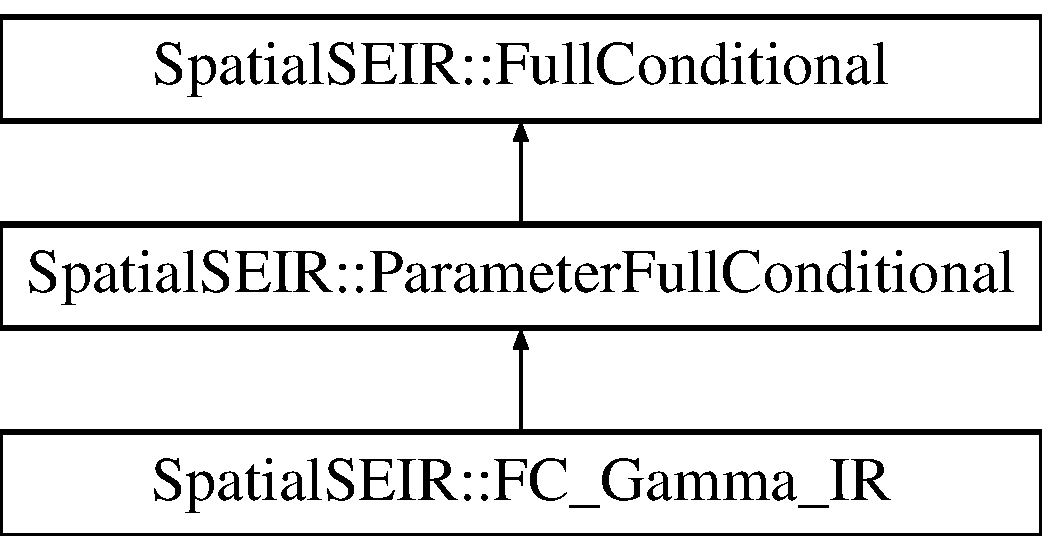
\includegraphics[height=3.000000cm]{classSpatialSEIR_1_1FC__Gamma__IR}
\end{center}
\end{figure}
\subsection*{Public Member Functions}
\begin{DoxyCompactItemize}
\item 
\hyperlink{classSpatialSEIR_1_1FC__Gamma__IR_ae561d9627dbbd79c3ed2140daebf7130}{F\-C\-\_\-\-Gamma\-\_\-\-I\-R} (\hyperlink{classSpatialSEIR_1_1ModelContext}{Model\-Context} $\ast$\-\_\-context, \hyperlink{classSpatialSEIR_1_1CompartmentalModelMatrix}{Compartmental\-Model\-Matrix} $\ast$\-\_\-\-R\-\_\-star, \hyperlink{classSpatialSEIR_1_1CompartmentalModelMatrix}{Compartmental\-Model\-Matrix} $\ast$\-\_\-\-I, \hyperlink{classSpatialSEIR_1_1InitData}{Init\-Data} $\ast$\-\_\-\-A0, double $\ast$\-\_\-p\-\_\-ir, double $\ast$\-\_\-gamma\-\_\-ir, double \-\_\-prior\-Alpha, double \-\_\-prior\-Beta, double \hyperlink{classSpatialSEIR_1_1FullConditional_a150ee031af8d086ad0a04b13630a110f}{slice\-Width})
\item 
\hyperlink{classSpatialSEIR_1_1FC__Gamma__IR_a749dee0018d26639f5973884bea96e0c}{$\sim$\-F\-C\-\_\-\-Gamma\-\_\-\-I\-R} ()
\item 
virtual double \hyperlink{classSpatialSEIR_1_1FC__Gamma__IR_a3615e9760812f273c3ccf901d5924c4a}{eval\-Prior} ()
\item 
virtual int \hyperlink{classSpatialSEIR_1_1FC__Gamma__IR_ac52b633a7878870a2e1adf059fb3c2ea}{eval\-C\-P\-U} ()
\item 
virtual int \hyperlink{classSpatialSEIR_1_1FC__Gamma__IR_a3423d47b7728892497a94407ecc37730}{eval\-O\-C\-L} ()
\item 
virtual void \hyperlink{classSpatialSEIR_1_1FC__Gamma__IR_a1067c9b99b419d8c9d3566a5eb4b6d73}{sample} (int verbose)
\item 
virtual long double \hyperlink{classSpatialSEIR_1_1FC__Gamma__IR_a0895a64e8292e75141a4ad9ed1145e9d}{get\-Value} ()
\item 
virtual void \hyperlink{classSpatialSEIR_1_1FC__Gamma__IR_a8517282f2fc24d52a00a426aa414f237}{set\-Value} (long double val)
\item 
virtual int \hyperlink{classSpatialSEIR_1_1FC__Gamma__IR_acdeddf0a6d53d2f10e7a12edf3924383}{calculate\-Relevant\-Compartments} ()
\item 
virtual int \hyperlink{classSpatialSEIR_1_1FC__Gamma__IR_a200f28e508a37bd50a8a0155fcd467c6}{calculate\-Relevant\-Compartments\-\_\-\-O\-C\-L} ()
\end{DoxyCompactItemize}
\subsection*{Public Attributes}
\begin{DoxyCompactItemize}
\item 
\hyperlink{classSpatialSEIR_1_1ModelContext}{Model\-Context} $\ast$$\ast$ \hyperlink{classSpatialSEIR_1_1FC__Gamma__IR_a424028d886dfc9bf9ca5b5e738d42549}{context}
\item 
\hyperlink{classSpatialSEIR_1_1CompartmentalModelMatrix}{Compartmental\-Model\-Matrix} $\ast$$\ast$ \hyperlink{classSpatialSEIR_1_1FC__Gamma__IR_a089d9691a6ae010f883de506686ff813}{R\-\_\-star}
\item 
\hyperlink{classSpatialSEIR_1_1CompartmentalModelMatrix}{Compartmental\-Model\-Matrix} $\ast$$\ast$ \hyperlink{classSpatialSEIR_1_1FC__Gamma__IR_abe3e9d16aa960008aa14709a55972606}{I}
\item 
\hyperlink{classSpatialSEIR_1_1InitData}{Init\-Data} $\ast$$\ast$ \hyperlink{classSpatialSEIR_1_1FC__Gamma__IR_aec7fb5f5d1fa9325c1f6c464d9edd121}{A0}
\item 
double $\ast$$\ast$ \hyperlink{classSpatialSEIR_1_1FC__Gamma__IR_ae1109fa525f1c3a8ceca2f4fbb955bb5}{p\-\_\-ir}
\item 
double $\ast$$\ast$ \hyperlink{classSpatialSEIR_1_1FC__Gamma__IR_a59115dead1bcf07b3839241a27be4c37}{gamma\-\_\-ir}
\item 
long double $\ast$ \hyperlink{classSpatialSEIR_1_1FC__Gamma__IR_ac34f1496de3501478a9915cc8930f56c}{value}
\item 
double $\ast$ \hyperlink{classSpatialSEIR_1_1FC__Gamma__IR_a17f5b19b6b11baa0befae17c2981789c}{prior\-Alpha}
\item 
double $\ast$ \hyperlink{classSpatialSEIR_1_1FC__Gamma__IR_aab39045db2213fef0e91aa5b758d7024}{prior\-Beta}
\end{DoxyCompactItemize}


\subsection{Detailed Description}
\hyperlink{classSpatialSEIR_1_1FC__Gamma__IR}{F\-C\-\_\-\-Gamma\-\_\-\-I\-R} gives the full conditional distribution of gamma\-\_\-ir, the parameter driving the, probability that an infectious individual recovers/is removed at a given time point (p\-\_\-ir). 

\subsection{Constructor \& Destructor Documentation}
\hypertarget{classSpatialSEIR_1_1FC__Gamma__IR_ae561d9627dbbd79c3ed2140daebf7130}{\index{Spatial\-S\-E\-I\-R\-::\-F\-C\-\_\-\-Gamma\-\_\-\-I\-R@{Spatial\-S\-E\-I\-R\-::\-F\-C\-\_\-\-Gamma\-\_\-\-I\-R}!F\-C\-\_\-\-Gamma\-\_\-\-I\-R@{F\-C\-\_\-\-Gamma\-\_\-\-I\-R}}
\index{F\-C\-\_\-\-Gamma\-\_\-\-I\-R@{F\-C\-\_\-\-Gamma\-\_\-\-I\-R}!SpatialSEIR::FC_Gamma_IR@{Spatial\-S\-E\-I\-R\-::\-F\-C\-\_\-\-Gamma\-\_\-\-I\-R}}
\subsubsection[{F\-C\-\_\-\-Gamma\-\_\-\-I\-R}]{\setlength{\rightskip}{0pt plus 5cm}Spatial\-S\-E\-I\-R\-::\-F\-C\-\_\-\-Gamma\-\_\-\-I\-R\-::\-F\-C\-\_\-\-Gamma\-\_\-\-I\-R (
\begin{DoxyParamCaption}
\item[{{\bf Model\-Context} $\ast$}]{\-\_\-context, }
\item[{{\bf Compartmental\-Model\-Matrix} $\ast$}]{\-\_\-\-R\-\_\-star, }
\item[{{\bf Compartmental\-Model\-Matrix} $\ast$}]{\-\_\-\-I, }
\item[{{\bf Init\-Data} $\ast$}]{\-\_\-\-A0, }
\item[{double $\ast$}]{\-\_\-p\-\_\-ir, }
\item[{double $\ast$}]{\-\_\-gamma\-\_\-ir, }
\item[{double}]{\-\_\-prior\-Alpha, }
\item[{double}]{\-\_\-prior\-Beta, }
\item[{double}]{slice\-Width}
\end{DoxyParamCaption}
)}}\label{classSpatialSEIR_1_1FC__Gamma__IR_ae561d9627dbbd79c3ed2140daebf7130}
\hypertarget{classSpatialSEIR_1_1FC__Gamma__IR_a749dee0018d26639f5973884bea96e0c}{\index{Spatial\-S\-E\-I\-R\-::\-F\-C\-\_\-\-Gamma\-\_\-\-I\-R@{Spatial\-S\-E\-I\-R\-::\-F\-C\-\_\-\-Gamma\-\_\-\-I\-R}!$\sim$\-F\-C\-\_\-\-Gamma\-\_\-\-I\-R@{$\sim$\-F\-C\-\_\-\-Gamma\-\_\-\-I\-R}}
\index{$\sim$\-F\-C\-\_\-\-Gamma\-\_\-\-I\-R@{$\sim$\-F\-C\-\_\-\-Gamma\-\_\-\-I\-R}!SpatialSEIR::FC_Gamma_IR@{Spatial\-S\-E\-I\-R\-::\-F\-C\-\_\-\-Gamma\-\_\-\-I\-R}}
\subsubsection[{$\sim$\-F\-C\-\_\-\-Gamma\-\_\-\-I\-R}]{\setlength{\rightskip}{0pt plus 5cm}Spatial\-S\-E\-I\-R\-::\-F\-C\-\_\-\-Gamma\-\_\-\-I\-R\-::$\sim$\-F\-C\-\_\-\-Gamma\-\_\-\-I\-R (
\begin{DoxyParamCaption}
{}
\end{DoxyParamCaption}
)}}\label{classSpatialSEIR_1_1FC__Gamma__IR_a749dee0018d26639f5973884bea96e0c}


\subsection{Member Function Documentation}
\hypertarget{classSpatialSEIR_1_1FC__Gamma__IR_acdeddf0a6d53d2f10e7a12edf3924383}{\index{Spatial\-S\-E\-I\-R\-::\-F\-C\-\_\-\-Gamma\-\_\-\-I\-R@{Spatial\-S\-E\-I\-R\-::\-F\-C\-\_\-\-Gamma\-\_\-\-I\-R}!calculate\-Relevant\-Compartments@{calculate\-Relevant\-Compartments}}
\index{calculate\-Relevant\-Compartments@{calculate\-Relevant\-Compartments}!SpatialSEIR::FC_Gamma_IR@{Spatial\-S\-E\-I\-R\-::\-F\-C\-\_\-\-Gamma\-\_\-\-I\-R}}
\subsubsection[{calculate\-Relevant\-Compartments}]{\setlength{\rightskip}{0pt plus 5cm}int Spatial\-S\-E\-I\-R\-::\-F\-C\-\_\-\-Gamma\-\_\-\-I\-R\-::calculate\-Relevant\-Compartments (
\begin{DoxyParamCaption}
{}
\end{DoxyParamCaption}
)\hspace{0.3cm}{\ttfamily [virtual]}}}\label{classSpatialSEIR_1_1FC__Gamma__IR_acdeddf0a6d53d2f10e7a12edf3924383}


Implements \hyperlink{classSpatialSEIR_1_1ParameterFullConditional_a65c39a2c3ca56e2f194b78cd362d35f9}{Spatial\-S\-E\-I\-R\-::\-Parameter\-Full\-Conditional}.

\hypertarget{classSpatialSEIR_1_1FC__Gamma__IR_a200f28e508a37bd50a8a0155fcd467c6}{\index{Spatial\-S\-E\-I\-R\-::\-F\-C\-\_\-\-Gamma\-\_\-\-I\-R@{Spatial\-S\-E\-I\-R\-::\-F\-C\-\_\-\-Gamma\-\_\-\-I\-R}!calculate\-Relevant\-Compartments\-\_\-\-O\-C\-L@{calculate\-Relevant\-Compartments\-\_\-\-O\-C\-L}}
\index{calculate\-Relevant\-Compartments\-\_\-\-O\-C\-L@{calculate\-Relevant\-Compartments\-\_\-\-O\-C\-L}!SpatialSEIR::FC_Gamma_IR@{Spatial\-S\-E\-I\-R\-::\-F\-C\-\_\-\-Gamma\-\_\-\-I\-R}}
\subsubsection[{calculate\-Relevant\-Compartments\-\_\-\-O\-C\-L}]{\setlength{\rightskip}{0pt plus 5cm}int Spatial\-S\-E\-I\-R\-::\-F\-C\-\_\-\-Gamma\-\_\-\-I\-R\-::calculate\-Relevant\-Compartments\-\_\-\-O\-C\-L (
\begin{DoxyParamCaption}
{}
\end{DoxyParamCaption}
)\hspace{0.3cm}{\ttfamily [virtual]}}}\label{classSpatialSEIR_1_1FC__Gamma__IR_a200f28e508a37bd50a8a0155fcd467c6}


Implements \hyperlink{classSpatialSEIR_1_1ParameterFullConditional_af40754537736a64f58848e0368b001fb}{Spatial\-S\-E\-I\-R\-::\-Parameter\-Full\-Conditional}.

\hypertarget{classSpatialSEIR_1_1FC__Gamma__IR_ac52b633a7878870a2e1adf059fb3c2ea}{\index{Spatial\-S\-E\-I\-R\-::\-F\-C\-\_\-\-Gamma\-\_\-\-I\-R@{Spatial\-S\-E\-I\-R\-::\-F\-C\-\_\-\-Gamma\-\_\-\-I\-R}!eval\-C\-P\-U@{eval\-C\-P\-U}}
\index{eval\-C\-P\-U@{eval\-C\-P\-U}!SpatialSEIR::FC_Gamma_IR@{Spatial\-S\-E\-I\-R\-::\-F\-C\-\_\-\-Gamma\-\_\-\-I\-R}}
\subsubsection[{eval\-C\-P\-U}]{\setlength{\rightskip}{0pt plus 5cm}int Spatial\-S\-E\-I\-R\-::\-F\-C\-\_\-\-Gamma\-\_\-\-I\-R\-::eval\-C\-P\-U (
\begin{DoxyParamCaption}
{}
\end{DoxyParamCaption}
)\hspace{0.3cm}{\ttfamily [virtual]}}}\label{classSpatialSEIR_1_1FC__Gamma__IR_ac52b633a7878870a2e1adf059fb3c2ea}


Implements \hyperlink{classSpatialSEIR_1_1ParameterFullConditional_a186bd19fdeb52ca4522f56fb880201dd}{Spatial\-S\-E\-I\-R\-::\-Parameter\-Full\-Conditional}.

\hypertarget{classSpatialSEIR_1_1FC__Gamma__IR_a3423d47b7728892497a94407ecc37730}{\index{Spatial\-S\-E\-I\-R\-::\-F\-C\-\_\-\-Gamma\-\_\-\-I\-R@{Spatial\-S\-E\-I\-R\-::\-F\-C\-\_\-\-Gamma\-\_\-\-I\-R}!eval\-O\-C\-L@{eval\-O\-C\-L}}
\index{eval\-O\-C\-L@{eval\-O\-C\-L}!SpatialSEIR::FC_Gamma_IR@{Spatial\-S\-E\-I\-R\-::\-F\-C\-\_\-\-Gamma\-\_\-\-I\-R}}
\subsubsection[{eval\-O\-C\-L}]{\setlength{\rightskip}{0pt plus 5cm}int Spatial\-S\-E\-I\-R\-::\-F\-C\-\_\-\-Gamma\-\_\-\-I\-R\-::eval\-O\-C\-L (
\begin{DoxyParamCaption}
{}
\end{DoxyParamCaption}
)\hspace{0.3cm}{\ttfamily [virtual]}}}\label{classSpatialSEIR_1_1FC__Gamma__IR_a3423d47b7728892497a94407ecc37730}


Implements \hyperlink{classSpatialSEIR_1_1ParameterFullConditional_ac4cfb13dace7f72e8136c45d9e959eec}{Spatial\-S\-E\-I\-R\-::\-Parameter\-Full\-Conditional}.

\hypertarget{classSpatialSEIR_1_1FC__Gamma__IR_a3615e9760812f273c3ccf901d5924c4a}{\index{Spatial\-S\-E\-I\-R\-::\-F\-C\-\_\-\-Gamma\-\_\-\-I\-R@{Spatial\-S\-E\-I\-R\-::\-F\-C\-\_\-\-Gamma\-\_\-\-I\-R}!eval\-Prior@{eval\-Prior}}
\index{eval\-Prior@{eval\-Prior}!SpatialSEIR::FC_Gamma_IR@{Spatial\-S\-E\-I\-R\-::\-F\-C\-\_\-\-Gamma\-\_\-\-I\-R}}
\subsubsection[{eval\-Prior}]{\setlength{\rightskip}{0pt plus 5cm}double Spatial\-S\-E\-I\-R\-::\-F\-C\-\_\-\-Gamma\-\_\-\-I\-R\-::eval\-Prior (
\begin{DoxyParamCaption}
{}
\end{DoxyParamCaption}
)\hspace{0.3cm}{\ttfamily [virtual]}}}\label{classSpatialSEIR_1_1FC__Gamma__IR_a3615e9760812f273c3ccf901d5924c4a}
\hypertarget{classSpatialSEIR_1_1FC__Gamma__IR_a0895a64e8292e75141a4ad9ed1145e9d}{\index{Spatial\-S\-E\-I\-R\-::\-F\-C\-\_\-\-Gamma\-\_\-\-I\-R@{Spatial\-S\-E\-I\-R\-::\-F\-C\-\_\-\-Gamma\-\_\-\-I\-R}!get\-Value@{get\-Value}}
\index{get\-Value@{get\-Value}!SpatialSEIR::FC_Gamma_IR@{Spatial\-S\-E\-I\-R\-::\-F\-C\-\_\-\-Gamma\-\_\-\-I\-R}}
\subsubsection[{get\-Value}]{\setlength{\rightskip}{0pt plus 5cm}long double Spatial\-S\-E\-I\-R\-::\-F\-C\-\_\-\-Gamma\-\_\-\-I\-R\-::get\-Value (
\begin{DoxyParamCaption}
{}
\end{DoxyParamCaption}
)\hspace{0.3cm}{\ttfamily [virtual]}}}\label{classSpatialSEIR_1_1FC__Gamma__IR_a0895a64e8292e75141a4ad9ed1145e9d}


Implements \hyperlink{classSpatialSEIR_1_1ParameterFullConditional_a901368d385809e77179b9fa7532adfec}{Spatial\-S\-E\-I\-R\-::\-Parameter\-Full\-Conditional}.

\hypertarget{classSpatialSEIR_1_1FC__Gamma__IR_a1067c9b99b419d8c9d3566a5eb4b6d73}{\index{Spatial\-S\-E\-I\-R\-::\-F\-C\-\_\-\-Gamma\-\_\-\-I\-R@{Spatial\-S\-E\-I\-R\-::\-F\-C\-\_\-\-Gamma\-\_\-\-I\-R}!sample@{sample}}
\index{sample@{sample}!SpatialSEIR::FC_Gamma_IR@{Spatial\-S\-E\-I\-R\-::\-F\-C\-\_\-\-Gamma\-\_\-\-I\-R}}
\subsubsection[{sample}]{\setlength{\rightskip}{0pt plus 5cm}void Spatial\-S\-E\-I\-R\-::\-F\-C\-\_\-\-Gamma\-\_\-\-I\-R\-::sample (
\begin{DoxyParamCaption}
\item[{int}]{verbose}
\end{DoxyParamCaption}
)\hspace{0.3cm}{\ttfamily [virtual]}}}\label{classSpatialSEIR_1_1FC__Gamma__IR_a1067c9b99b419d8c9d3566a5eb4b6d73}


Implements \hyperlink{classSpatialSEIR_1_1ParameterFullConditional_a651e22b15782acb6bd80be12bd476693}{Spatial\-S\-E\-I\-R\-::\-Parameter\-Full\-Conditional}.

\hypertarget{classSpatialSEIR_1_1FC__Gamma__IR_a8517282f2fc24d52a00a426aa414f237}{\index{Spatial\-S\-E\-I\-R\-::\-F\-C\-\_\-\-Gamma\-\_\-\-I\-R@{Spatial\-S\-E\-I\-R\-::\-F\-C\-\_\-\-Gamma\-\_\-\-I\-R}!set\-Value@{set\-Value}}
\index{set\-Value@{set\-Value}!SpatialSEIR::FC_Gamma_IR@{Spatial\-S\-E\-I\-R\-::\-F\-C\-\_\-\-Gamma\-\_\-\-I\-R}}
\subsubsection[{set\-Value}]{\setlength{\rightskip}{0pt plus 5cm}void Spatial\-S\-E\-I\-R\-::\-F\-C\-\_\-\-Gamma\-\_\-\-I\-R\-::set\-Value (
\begin{DoxyParamCaption}
\item[{long double}]{val}
\end{DoxyParamCaption}
)\hspace{0.3cm}{\ttfamily [virtual]}}}\label{classSpatialSEIR_1_1FC__Gamma__IR_a8517282f2fc24d52a00a426aa414f237}


Implements \hyperlink{classSpatialSEIR_1_1ParameterFullConditional_adf03f213e27d26f120b574d6dd86ffc3}{Spatial\-S\-E\-I\-R\-::\-Parameter\-Full\-Conditional}.



\subsection{Member Data Documentation}
\hypertarget{classSpatialSEIR_1_1FC__Gamma__IR_aec7fb5f5d1fa9325c1f6c464d9edd121}{\index{Spatial\-S\-E\-I\-R\-::\-F\-C\-\_\-\-Gamma\-\_\-\-I\-R@{Spatial\-S\-E\-I\-R\-::\-F\-C\-\_\-\-Gamma\-\_\-\-I\-R}!A0@{A0}}
\index{A0@{A0}!SpatialSEIR::FC_Gamma_IR@{Spatial\-S\-E\-I\-R\-::\-F\-C\-\_\-\-Gamma\-\_\-\-I\-R}}
\subsubsection[{A0}]{\setlength{\rightskip}{0pt plus 5cm}{\bf Init\-Data}$\ast$$\ast$ Spatial\-S\-E\-I\-R\-::\-F\-C\-\_\-\-Gamma\-\_\-\-I\-R\-::\-A0}}\label{classSpatialSEIR_1_1FC__Gamma__IR_aec7fb5f5d1fa9325c1f6c464d9edd121}
\hypertarget{classSpatialSEIR_1_1FC__Gamma__IR_a424028d886dfc9bf9ca5b5e738d42549}{\index{Spatial\-S\-E\-I\-R\-::\-F\-C\-\_\-\-Gamma\-\_\-\-I\-R@{Spatial\-S\-E\-I\-R\-::\-F\-C\-\_\-\-Gamma\-\_\-\-I\-R}!context@{context}}
\index{context@{context}!SpatialSEIR::FC_Gamma_IR@{Spatial\-S\-E\-I\-R\-::\-F\-C\-\_\-\-Gamma\-\_\-\-I\-R}}
\subsubsection[{context}]{\setlength{\rightskip}{0pt plus 5cm}{\bf Model\-Context}$\ast$$\ast$ Spatial\-S\-E\-I\-R\-::\-F\-C\-\_\-\-Gamma\-\_\-\-I\-R\-::context}}\label{classSpatialSEIR_1_1FC__Gamma__IR_a424028d886dfc9bf9ca5b5e738d42549}
\hypertarget{classSpatialSEIR_1_1FC__Gamma__IR_a59115dead1bcf07b3839241a27be4c37}{\index{Spatial\-S\-E\-I\-R\-::\-F\-C\-\_\-\-Gamma\-\_\-\-I\-R@{Spatial\-S\-E\-I\-R\-::\-F\-C\-\_\-\-Gamma\-\_\-\-I\-R}!gamma\-\_\-ir@{gamma\-\_\-ir}}
\index{gamma\-\_\-ir@{gamma\-\_\-ir}!SpatialSEIR::FC_Gamma_IR@{Spatial\-S\-E\-I\-R\-::\-F\-C\-\_\-\-Gamma\-\_\-\-I\-R}}
\subsubsection[{gamma\-\_\-ir}]{\setlength{\rightskip}{0pt plus 5cm}double$\ast$$\ast$ Spatial\-S\-E\-I\-R\-::\-F\-C\-\_\-\-Gamma\-\_\-\-I\-R\-::gamma\-\_\-ir}}\label{classSpatialSEIR_1_1FC__Gamma__IR_a59115dead1bcf07b3839241a27be4c37}
\hypertarget{classSpatialSEIR_1_1FC__Gamma__IR_abe3e9d16aa960008aa14709a55972606}{\index{Spatial\-S\-E\-I\-R\-::\-F\-C\-\_\-\-Gamma\-\_\-\-I\-R@{Spatial\-S\-E\-I\-R\-::\-F\-C\-\_\-\-Gamma\-\_\-\-I\-R}!I@{I}}
\index{I@{I}!SpatialSEIR::FC_Gamma_IR@{Spatial\-S\-E\-I\-R\-::\-F\-C\-\_\-\-Gamma\-\_\-\-I\-R}}
\subsubsection[{I}]{\setlength{\rightskip}{0pt plus 5cm}{\bf Compartmental\-Model\-Matrix}$\ast$$\ast$ Spatial\-S\-E\-I\-R\-::\-F\-C\-\_\-\-Gamma\-\_\-\-I\-R\-::\-I}}\label{classSpatialSEIR_1_1FC__Gamma__IR_abe3e9d16aa960008aa14709a55972606}
\hypertarget{classSpatialSEIR_1_1FC__Gamma__IR_ae1109fa525f1c3a8ceca2f4fbb955bb5}{\index{Spatial\-S\-E\-I\-R\-::\-F\-C\-\_\-\-Gamma\-\_\-\-I\-R@{Spatial\-S\-E\-I\-R\-::\-F\-C\-\_\-\-Gamma\-\_\-\-I\-R}!p\-\_\-ir@{p\-\_\-ir}}
\index{p\-\_\-ir@{p\-\_\-ir}!SpatialSEIR::FC_Gamma_IR@{Spatial\-S\-E\-I\-R\-::\-F\-C\-\_\-\-Gamma\-\_\-\-I\-R}}
\subsubsection[{p\-\_\-ir}]{\setlength{\rightskip}{0pt plus 5cm}double$\ast$$\ast$ Spatial\-S\-E\-I\-R\-::\-F\-C\-\_\-\-Gamma\-\_\-\-I\-R\-::p\-\_\-ir}}\label{classSpatialSEIR_1_1FC__Gamma__IR_ae1109fa525f1c3a8ceca2f4fbb955bb5}
\hypertarget{classSpatialSEIR_1_1FC__Gamma__IR_a17f5b19b6b11baa0befae17c2981789c}{\index{Spatial\-S\-E\-I\-R\-::\-F\-C\-\_\-\-Gamma\-\_\-\-I\-R@{Spatial\-S\-E\-I\-R\-::\-F\-C\-\_\-\-Gamma\-\_\-\-I\-R}!prior\-Alpha@{prior\-Alpha}}
\index{prior\-Alpha@{prior\-Alpha}!SpatialSEIR::FC_Gamma_IR@{Spatial\-S\-E\-I\-R\-::\-F\-C\-\_\-\-Gamma\-\_\-\-I\-R}}
\subsubsection[{prior\-Alpha}]{\setlength{\rightskip}{0pt plus 5cm}double$\ast$ Spatial\-S\-E\-I\-R\-::\-F\-C\-\_\-\-Gamma\-\_\-\-I\-R\-::prior\-Alpha}}\label{classSpatialSEIR_1_1FC__Gamma__IR_a17f5b19b6b11baa0befae17c2981789c}
\hypertarget{classSpatialSEIR_1_1FC__Gamma__IR_aab39045db2213fef0e91aa5b758d7024}{\index{Spatial\-S\-E\-I\-R\-::\-F\-C\-\_\-\-Gamma\-\_\-\-I\-R@{Spatial\-S\-E\-I\-R\-::\-F\-C\-\_\-\-Gamma\-\_\-\-I\-R}!prior\-Beta@{prior\-Beta}}
\index{prior\-Beta@{prior\-Beta}!SpatialSEIR::FC_Gamma_IR@{Spatial\-S\-E\-I\-R\-::\-F\-C\-\_\-\-Gamma\-\_\-\-I\-R}}
\subsubsection[{prior\-Beta}]{\setlength{\rightskip}{0pt plus 5cm}double$\ast$ Spatial\-S\-E\-I\-R\-::\-F\-C\-\_\-\-Gamma\-\_\-\-I\-R\-::prior\-Beta}}\label{classSpatialSEIR_1_1FC__Gamma__IR_aab39045db2213fef0e91aa5b758d7024}
\hypertarget{classSpatialSEIR_1_1FC__Gamma__IR_a089d9691a6ae010f883de506686ff813}{\index{Spatial\-S\-E\-I\-R\-::\-F\-C\-\_\-\-Gamma\-\_\-\-I\-R@{Spatial\-S\-E\-I\-R\-::\-F\-C\-\_\-\-Gamma\-\_\-\-I\-R}!R\-\_\-star@{R\-\_\-star}}
\index{R\-\_\-star@{R\-\_\-star}!SpatialSEIR::FC_Gamma_IR@{Spatial\-S\-E\-I\-R\-::\-F\-C\-\_\-\-Gamma\-\_\-\-I\-R}}
\subsubsection[{R\-\_\-star}]{\setlength{\rightskip}{0pt plus 5cm}{\bf Compartmental\-Model\-Matrix}$\ast$$\ast$ Spatial\-S\-E\-I\-R\-::\-F\-C\-\_\-\-Gamma\-\_\-\-I\-R\-::\-R\-\_\-star}}\label{classSpatialSEIR_1_1FC__Gamma__IR_a089d9691a6ae010f883de506686ff813}
\hypertarget{classSpatialSEIR_1_1FC__Gamma__IR_ac34f1496de3501478a9915cc8930f56c}{\index{Spatial\-S\-E\-I\-R\-::\-F\-C\-\_\-\-Gamma\-\_\-\-I\-R@{Spatial\-S\-E\-I\-R\-::\-F\-C\-\_\-\-Gamma\-\_\-\-I\-R}!value@{value}}
\index{value@{value}!SpatialSEIR::FC_Gamma_IR@{Spatial\-S\-E\-I\-R\-::\-F\-C\-\_\-\-Gamma\-\_\-\-I\-R}}
\subsubsection[{value}]{\setlength{\rightskip}{0pt plus 5cm}long double$\ast$ Spatial\-S\-E\-I\-R\-::\-F\-C\-\_\-\-Gamma\-\_\-\-I\-R\-::value}}\label{classSpatialSEIR_1_1FC__Gamma__IR_ac34f1496de3501478a9915cc8930f56c}


The documentation for this class was generated from the following files\-:\begin{DoxyCompactItemize}
\item 
lib\-Spatial\-S\-E\-I\-R/include/\-Full\-Conditionals/\hyperlink{LSS__FC__Gamma__IR_8hpp}{L\-S\-S\-\_\-\-F\-C\-\_\-\-Gamma\-\_\-\-I\-R.\-hpp}\item 
lib\-Spatial\-S\-E\-I\-R/src/\-Full\-Conditionals/\hyperlink{FC__Gamma__IR_8cpp}{F\-C\-\_\-\-Gamma\-\_\-\-I\-R.\-cpp}\end{DoxyCompactItemize}

\hypertarget{classSpatialSEIR_1_1FC__I0}{\section{Spatial\-S\-E\-I\-R\-:\-:F\-C\-\_\-\-I0 Class Reference}
\label{classSpatialSEIR_1_1FC__I0}\index{Spatial\-S\-E\-I\-R\-::\-F\-C\-\_\-\-I0@{Spatial\-S\-E\-I\-R\-::\-F\-C\-\_\-\-I0}}
}


{\ttfamily \#include $<$L\-S\-S\-\_\-\-F\-C\-\_\-\-I0.\-hpp$>$}

Inheritance diagram for Spatial\-S\-E\-I\-R\-:\-:F\-C\-\_\-\-I0\-:\begin{figure}[H]
\begin{center}
\leavevmode
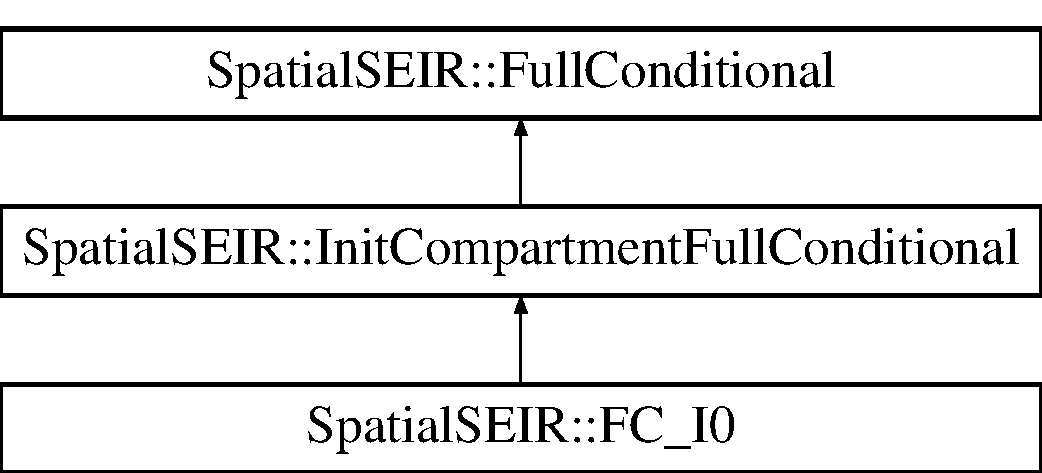
\includegraphics[height=3.000000cm]{classSpatialSEIR_1_1FC__I0}
\end{center}
\end{figure}
\subsection*{Public Member Functions}
\begin{DoxyCompactItemize}
\item 
\hyperlink{classSpatialSEIR_1_1FC__I0_a3b6918878122f5499f9daa03732580e0}{F\-C\-\_\-\-I0} (\hyperlink{classSpatialSEIR_1_1ModelContext}{Model\-Context} $\ast$\-\_\-context, \hyperlink{classSpatialSEIR_1_1CompartmentalModelMatrix}{Compartmental\-Model\-Matrix} $\ast$\-\_\-\-S, \hyperlink{classSpatialSEIR_1_1CompartmentalModelMatrix}{Compartmental\-Model\-Matrix} $\ast$\-\_\-\-I, \hyperlink{classSpatialSEIR_1_1CompartmentalModelMatrix}{Compartmental\-Model\-Matrix} $\ast$\-\_\-\-R, \hyperlink{classSpatialSEIR_1_1CompartmentalModelMatrix}{Compartmental\-Model\-Matrix} $\ast$\-\_\-\-S\-\_\-star, \hyperlink{classSpatialSEIR_1_1CompartmentalModelMatrix}{Compartmental\-Model\-Matrix} $\ast$\-\_\-\-E\-\_\-star, \hyperlink{classSpatialSEIR_1_1CompartmentalModelMatrix}{Compartmental\-Model\-Matrix} $\ast$\-\_\-\-R\-\_\-star, \hyperlink{classSpatialSEIR_1_1InitData}{Init\-Data} $\ast$\-\_\-\-A0, double $\ast$\-\_\-p\-\_\-ir, double $\ast$\-\_\-p\-\_\-rs, double $\ast$\-\_\-p\-\_\-se, double \hyperlink{classSpatialSEIR_1_1FullConditional_a150ee031af8d086ad0a04b13630a110f}{slice\-Width})
\item 
virtual \hyperlink{classSpatialSEIR_1_1FC__I0_a2260d07e48a7d7b5dab19ee22e365b38}{$\sim$\-F\-C\-\_\-\-I0} ()
\item 
virtual int \hyperlink{classSpatialSEIR_1_1FC__I0_a36dbaf498cb226c7b2042438f9432ae4}{eval\-C\-P\-U} ()
\item 
virtual int \hyperlink{classSpatialSEIR_1_1FC__I0_abc02f4b767cda97f040e53095dd3024d}{eval\-O\-C\-L} ()
\item 
virtual void \hyperlink{classSpatialSEIR_1_1FC__I0_af87aa3379ff282e36478301ff271ba40}{sample} (int verbose)
\item 
virtual long double \hyperlink{classSpatialSEIR_1_1FC__I0_a69f4e641113c47ae2e28dbd44f8c8261}{get\-Value} ()
\item 
virtual void \hyperlink{classSpatialSEIR_1_1FC__I0_ae5db486bbdcdf2900278a17aea761e7a}{set\-Value} (long double \hyperlink{classSpatialSEIR_1_1FC__I0_a81955b1dfdaf09a58122944420b40750}{value})
\item 
virtual int \hyperlink{classSpatialSEIR_1_1FC__I0_aa463dde280304445e22a9653536a1edb}{calculate\-Relevant\-Compartments} ()
\item 
virtual int \hyperlink{classSpatialSEIR_1_1FC__I0_ab1d7728b636f695a984ce609de87efde}{calculate\-Relevant\-Compartments\-\_\-\-O\-C\-L} ()
\end{DoxyCompactItemize}
\subsection*{Public Attributes}
\begin{DoxyCompactItemize}
\item 
\hyperlink{classSpatialSEIR_1_1ModelContext}{Model\-Context} $\ast$$\ast$ \hyperlink{classSpatialSEIR_1_1FC__I0_aec6c021bd72108821299dca140ec8b6e}{context}
\item 
\hyperlink{classSpatialSEIR_1_1CompartmentalModelMatrix}{Compartmental\-Model\-Matrix} $\ast$$\ast$ \hyperlink{classSpatialSEIR_1_1FC__I0_a32d56d02b4f1cc6a1394104cc45d6d5d}{S}
\item 
\hyperlink{classSpatialSEIR_1_1CompartmentalModelMatrix}{Compartmental\-Model\-Matrix} $\ast$$\ast$ \hyperlink{classSpatialSEIR_1_1FC__I0_abed267a2d412d94515c38468b4995297}{I}
\item 
\hyperlink{classSpatialSEIR_1_1CompartmentalModelMatrix}{Compartmental\-Model\-Matrix} $\ast$$\ast$ \hyperlink{classSpatialSEIR_1_1FC__I0_a6e9167bd8ec8794cc413b1109317f23e}{R}
\item 
\hyperlink{classSpatialSEIR_1_1CompartmentalModelMatrix}{Compartmental\-Model\-Matrix} $\ast$$\ast$ \hyperlink{classSpatialSEIR_1_1FC__I0_ad631c68300d51c2866204a5486706c0b}{S\-\_\-star}
\item 
\hyperlink{classSpatialSEIR_1_1CompartmentalModelMatrix}{Compartmental\-Model\-Matrix} $\ast$$\ast$ \hyperlink{classSpatialSEIR_1_1FC__I0_a671eca4d02352fd5cd3a1c2a2960c5cf}{E\-\_\-star}
\item 
\hyperlink{classSpatialSEIR_1_1CompartmentalModelMatrix}{Compartmental\-Model\-Matrix} $\ast$$\ast$ \hyperlink{classSpatialSEIR_1_1FC__I0_a70a7f699e9da71d33ed74c27747c69d1}{R\-\_\-star}
\item 
\hyperlink{classSpatialSEIR_1_1InitData}{Init\-Data} $\ast$$\ast$ \hyperlink{classSpatialSEIR_1_1FC__I0_a30c65326a76d65ed05040aa32fd1385c}{A0}
\item 
double $\ast$$\ast$ \hyperlink{classSpatialSEIR_1_1FC__I0_ae21756cfc313d026a673343ce736e79f}{p\-\_\-ir}
\item 
double $\ast$$\ast$ \hyperlink{classSpatialSEIR_1_1FC__I0_a42de4548f29af1c2e2d9409d58a2af12}{p\-\_\-rs}
\item 
double $\ast$$\ast$ \hyperlink{classSpatialSEIR_1_1FC__I0_a9708209e3d96f2f19762c5ce5e6da13f}{p\-\_\-se}
\item 
long double $\ast$ \hyperlink{classSpatialSEIR_1_1FC__I0_a81955b1dfdaf09a58122944420b40750}{value}
\end{DoxyCompactItemize}


\subsection{Detailed Description}
\hyperlink{classSpatialSEIR_1_1FC__I0}{F\-C\-\_\-\-I0} gives the full conditional distribution for the vector of initially infectious individuals. 

\subsection{Constructor \& Destructor Documentation}
\hypertarget{classSpatialSEIR_1_1FC__I0_a3b6918878122f5499f9daa03732580e0}{\index{Spatial\-S\-E\-I\-R\-::\-F\-C\-\_\-\-I0@{Spatial\-S\-E\-I\-R\-::\-F\-C\-\_\-\-I0}!F\-C\-\_\-\-I0@{F\-C\-\_\-\-I0}}
\index{F\-C\-\_\-\-I0@{F\-C\-\_\-\-I0}!SpatialSEIR::FC_I0@{Spatial\-S\-E\-I\-R\-::\-F\-C\-\_\-\-I0}}
\subsubsection[{F\-C\-\_\-\-I0}]{\setlength{\rightskip}{0pt plus 5cm}Spatial\-S\-E\-I\-R\-::\-F\-C\-\_\-\-I0\-::\-F\-C\-\_\-\-I0 (
\begin{DoxyParamCaption}
\item[{{\bf Model\-Context} $\ast$}]{\-\_\-context, }
\item[{{\bf Compartmental\-Model\-Matrix} $\ast$}]{\-\_\-\-S, }
\item[{{\bf Compartmental\-Model\-Matrix} $\ast$}]{\-\_\-\-I, }
\item[{{\bf Compartmental\-Model\-Matrix} $\ast$}]{\-\_\-\-R, }
\item[{{\bf Compartmental\-Model\-Matrix} $\ast$}]{\-\_\-\-S\-\_\-star, }
\item[{{\bf Compartmental\-Model\-Matrix} $\ast$}]{\-\_\-\-E\-\_\-star, }
\item[{{\bf Compartmental\-Model\-Matrix} $\ast$}]{\-\_\-\-R\-\_\-star, }
\item[{{\bf Init\-Data} $\ast$}]{\-\_\-\-A0, }
\item[{double $\ast$}]{\-\_\-p\-\_\-ir, }
\item[{double $\ast$}]{\-\_\-p\-\_\-rs, }
\item[{double $\ast$}]{\-\_\-p\-\_\-se, }
\item[{double}]{slice\-Width}
\end{DoxyParamCaption}
)}}\label{classSpatialSEIR_1_1FC__I0_a3b6918878122f5499f9daa03732580e0}
\hypertarget{classSpatialSEIR_1_1FC__I0_a2260d07e48a7d7b5dab19ee22e365b38}{\index{Spatial\-S\-E\-I\-R\-::\-F\-C\-\_\-\-I0@{Spatial\-S\-E\-I\-R\-::\-F\-C\-\_\-\-I0}!$\sim$\-F\-C\-\_\-\-I0@{$\sim$\-F\-C\-\_\-\-I0}}
\index{$\sim$\-F\-C\-\_\-\-I0@{$\sim$\-F\-C\-\_\-\-I0}!SpatialSEIR::FC_I0@{Spatial\-S\-E\-I\-R\-::\-F\-C\-\_\-\-I0}}
\subsubsection[{$\sim$\-F\-C\-\_\-\-I0}]{\setlength{\rightskip}{0pt plus 5cm}Spatial\-S\-E\-I\-R\-::\-F\-C\-\_\-\-I0\-::$\sim$\-F\-C\-\_\-\-I0 (
\begin{DoxyParamCaption}
{}
\end{DoxyParamCaption}
)\hspace{0.3cm}{\ttfamily [virtual]}}}\label{classSpatialSEIR_1_1FC__I0_a2260d07e48a7d7b5dab19ee22e365b38}


\subsection{Member Function Documentation}
\hypertarget{classSpatialSEIR_1_1FC__I0_aa463dde280304445e22a9653536a1edb}{\index{Spatial\-S\-E\-I\-R\-::\-F\-C\-\_\-\-I0@{Spatial\-S\-E\-I\-R\-::\-F\-C\-\_\-\-I0}!calculate\-Relevant\-Compartments@{calculate\-Relevant\-Compartments}}
\index{calculate\-Relevant\-Compartments@{calculate\-Relevant\-Compartments}!SpatialSEIR::FC_I0@{Spatial\-S\-E\-I\-R\-::\-F\-C\-\_\-\-I0}}
\subsubsection[{calculate\-Relevant\-Compartments}]{\setlength{\rightskip}{0pt plus 5cm}int Spatial\-S\-E\-I\-R\-::\-F\-C\-\_\-\-I0\-::calculate\-Relevant\-Compartments (
\begin{DoxyParamCaption}
{}
\end{DoxyParamCaption}
)\hspace{0.3cm}{\ttfamily [virtual]}}}\label{classSpatialSEIR_1_1FC__I0_aa463dde280304445e22a9653536a1edb}


Implements \hyperlink{classSpatialSEIR_1_1InitCompartmentFullConditional_a3fab33c4f5b857998fd928a00cea09e7}{Spatial\-S\-E\-I\-R\-::\-Init\-Compartment\-Full\-Conditional}.

\hypertarget{classSpatialSEIR_1_1FC__I0_ab1d7728b636f695a984ce609de87efde}{\index{Spatial\-S\-E\-I\-R\-::\-F\-C\-\_\-\-I0@{Spatial\-S\-E\-I\-R\-::\-F\-C\-\_\-\-I0}!calculate\-Relevant\-Compartments\-\_\-\-O\-C\-L@{calculate\-Relevant\-Compartments\-\_\-\-O\-C\-L}}
\index{calculate\-Relevant\-Compartments\-\_\-\-O\-C\-L@{calculate\-Relevant\-Compartments\-\_\-\-O\-C\-L}!SpatialSEIR::FC_I0@{Spatial\-S\-E\-I\-R\-::\-F\-C\-\_\-\-I0}}
\subsubsection[{calculate\-Relevant\-Compartments\-\_\-\-O\-C\-L}]{\setlength{\rightskip}{0pt plus 5cm}int Spatial\-S\-E\-I\-R\-::\-F\-C\-\_\-\-I0\-::calculate\-Relevant\-Compartments\-\_\-\-O\-C\-L (
\begin{DoxyParamCaption}
{}
\end{DoxyParamCaption}
)\hspace{0.3cm}{\ttfamily [virtual]}}}\label{classSpatialSEIR_1_1FC__I0_ab1d7728b636f695a984ce609de87efde}


Implements \hyperlink{classSpatialSEIR_1_1InitCompartmentFullConditional_aa4eae1aafbcdc4819be2e520d600dedf}{Spatial\-S\-E\-I\-R\-::\-Init\-Compartment\-Full\-Conditional}.

\hypertarget{classSpatialSEIR_1_1FC__I0_a36dbaf498cb226c7b2042438f9432ae4}{\index{Spatial\-S\-E\-I\-R\-::\-F\-C\-\_\-\-I0@{Spatial\-S\-E\-I\-R\-::\-F\-C\-\_\-\-I0}!eval\-C\-P\-U@{eval\-C\-P\-U}}
\index{eval\-C\-P\-U@{eval\-C\-P\-U}!SpatialSEIR::FC_I0@{Spatial\-S\-E\-I\-R\-::\-F\-C\-\_\-\-I0}}
\subsubsection[{eval\-C\-P\-U}]{\setlength{\rightskip}{0pt plus 5cm}int Spatial\-S\-E\-I\-R\-::\-F\-C\-\_\-\-I0\-::eval\-C\-P\-U (
\begin{DoxyParamCaption}
{}
\end{DoxyParamCaption}
)\hspace{0.3cm}{\ttfamily [virtual]}}}\label{classSpatialSEIR_1_1FC__I0_a36dbaf498cb226c7b2042438f9432ae4}


Implements \hyperlink{classSpatialSEIR_1_1InitCompartmentFullConditional_a25fc6e3ac2cb71a6e115ce3235fd8de0}{Spatial\-S\-E\-I\-R\-::\-Init\-Compartment\-Full\-Conditional}.

\hypertarget{classSpatialSEIR_1_1FC__I0_abc02f4b767cda97f040e53095dd3024d}{\index{Spatial\-S\-E\-I\-R\-::\-F\-C\-\_\-\-I0@{Spatial\-S\-E\-I\-R\-::\-F\-C\-\_\-\-I0}!eval\-O\-C\-L@{eval\-O\-C\-L}}
\index{eval\-O\-C\-L@{eval\-O\-C\-L}!SpatialSEIR::FC_I0@{Spatial\-S\-E\-I\-R\-::\-F\-C\-\_\-\-I0}}
\subsubsection[{eval\-O\-C\-L}]{\setlength{\rightskip}{0pt plus 5cm}int Spatial\-S\-E\-I\-R\-::\-F\-C\-\_\-\-I0\-::eval\-O\-C\-L (
\begin{DoxyParamCaption}
{}
\end{DoxyParamCaption}
)\hspace{0.3cm}{\ttfamily [virtual]}}}\label{classSpatialSEIR_1_1FC__I0_abc02f4b767cda97f040e53095dd3024d}


Implements \hyperlink{classSpatialSEIR_1_1InitCompartmentFullConditional_a2f0c4b5628e2f2074c1a84ea6349a754}{Spatial\-S\-E\-I\-R\-::\-Init\-Compartment\-Full\-Conditional}.

\hypertarget{classSpatialSEIR_1_1FC__I0_a69f4e641113c47ae2e28dbd44f8c8261}{\index{Spatial\-S\-E\-I\-R\-::\-F\-C\-\_\-\-I0@{Spatial\-S\-E\-I\-R\-::\-F\-C\-\_\-\-I0}!get\-Value@{get\-Value}}
\index{get\-Value@{get\-Value}!SpatialSEIR::FC_I0@{Spatial\-S\-E\-I\-R\-::\-F\-C\-\_\-\-I0}}
\subsubsection[{get\-Value}]{\setlength{\rightskip}{0pt plus 5cm}long double Spatial\-S\-E\-I\-R\-::\-F\-C\-\_\-\-I0\-::get\-Value (
\begin{DoxyParamCaption}
{}
\end{DoxyParamCaption}
)\hspace{0.3cm}{\ttfamily [virtual]}}}\label{classSpatialSEIR_1_1FC__I0_a69f4e641113c47ae2e28dbd44f8c8261}


Implements \hyperlink{classSpatialSEIR_1_1InitCompartmentFullConditional_aadb3975a791221136e6c4be5e016d9f1}{Spatial\-S\-E\-I\-R\-::\-Init\-Compartment\-Full\-Conditional}.

\hypertarget{classSpatialSEIR_1_1FC__I0_af87aa3379ff282e36478301ff271ba40}{\index{Spatial\-S\-E\-I\-R\-::\-F\-C\-\_\-\-I0@{Spatial\-S\-E\-I\-R\-::\-F\-C\-\_\-\-I0}!sample@{sample}}
\index{sample@{sample}!SpatialSEIR::FC_I0@{Spatial\-S\-E\-I\-R\-::\-F\-C\-\_\-\-I0}}
\subsubsection[{sample}]{\setlength{\rightskip}{0pt plus 5cm}void Spatial\-S\-E\-I\-R\-::\-F\-C\-\_\-\-I0\-::sample (
\begin{DoxyParamCaption}
\item[{int}]{verbose}
\end{DoxyParamCaption}
)\hspace{0.3cm}{\ttfamily [virtual]}}}\label{classSpatialSEIR_1_1FC__I0_af87aa3379ff282e36478301ff271ba40}


Implements \hyperlink{classSpatialSEIR_1_1InitCompartmentFullConditional_a03bcc440fa87265336980f3e833f59f2}{Spatial\-S\-E\-I\-R\-::\-Init\-Compartment\-Full\-Conditional}.

\hypertarget{classSpatialSEIR_1_1FC__I0_ae5db486bbdcdf2900278a17aea761e7a}{\index{Spatial\-S\-E\-I\-R\-::\-F\-C\-\_\-\-I0@{Spatial\-S\-E\-I\-R\-::\-F\-C\-\_\-\-I0}!set\-Value@{set\-Value}}
\index{set\-Value@{set\-Value}!SpatialSEIR::FC_I0@{Spatial\-S\-E\-I\-R\-::\-F\-C\-\_\-\-I0}}
\subsubsection[{set\-Value}]{\setlength{\rightskip}{0pt plus 5cm}void Spatial\-S\-E\-I\-R\-::\-F\-C\-\_\-\-I0\-::set\-Value (
\begin{DoxyParamCaption}
\item[{long double}]{value}
\end{DoxyParamCaption}
)\hspace{0.3cm}{\ttfamily [virtual]}}}\label{classSpatialSEIR_1_1FC__I0_ae5db486bbdcdf2900278a17aea761e7a}


Implements \hyperlink{classSpatialSEIR_1_1InitCompartmentFullConditional_acbc03a68f5c67beacefadcc3c22c1d88}{Spatial\-S\-E\-I\-R\-::\-Init\-Compartment\-Full\-Conditional}.



\subsection{Member Data Documentation}
\hypertarget{classSpatialSEIR_1_1FC__I0_a30c65326a76d65ed05040aa32fd1385c}{\index{Spatial\-S\-E\-I\-R\-::\-F\-C\-\_\-\-I0@{Spatial\-S\-E\-I\-R\-::\-F\-C\-\_\-\-I0}!A0@{A0}}
\index{A0@{A0}!SpatialSEIR::FC_I0@{Spatial\-S\-E\-I\-R\-::\-F\-C\-\_\-\-I0}}
\subsubsection[{A0}]{\setlength{\rightskip}{0pt plus 5cm}{\bf Init\-Data}$\ast$$\ast$ Spatial\-S\-E\-I\-R\-::\-F\-C\-\_\-\-I0\-::\-A0}}\label{classSpatialSEIR_1_1FC__I0_a30c65326a76d65ed05040aa32fd1385c}
\hypertarget{classSpatialSEIR_1_1FC__I0_aec6c021bd72108821299dca140ec8b6e}{\index{Spatial\-S\-E\-I\-R\-::\-F\-C\-\_\-\-I0@{Spatial\-S\-E\-I\-R\-::\-F\-C\-\_\-\-I0}!context@{context}}
\index{context@{context}!SpatialSEIR::FC_I0@{Spatial\-S\-E\-I\-R\-::\-F\-C\-\_\-\-I0}}
\subsubsection[{context}]{\setlength{\rightskip}{0pt plus 5cm}{\bf Model\-Context}$\ast$$\ast$ Spatial\-S\-E\-I\-R\-::\-F\-C\-\_\-\-I0\-::context}}\label{classSpatialSEIR_1_1FC__I0_aec6c021bd72108821299dca140ec8b6e}
\hypertarget{classSpatialSEIR_1_1FC__I0_a671eca4d02352fd5cd3a1c2a2960c5cf}{\index{Spatial\-S\-E\-I\-R\-::\-F\-C\-\_\-\-I0@{Spatial\-S\-E\-I\-R\-::\-F\-C\-\_\-\-I0}!E\-\_\-star@{E\-\_\-star}}
\index{E\-\_\-star@{E\-\_\-star}!SpatialSEIR::FC_I0@{Spatial\-S\-E\-I\-R\-::\-F\-C\-\_\-\-I0}}
\subsubsection[{E\-\_\-star}]{\setlength{\rightskip}{0pt plus 5cm}{\bf Compartmental\-Model\-Matrix}$\ast$$\ast$ Spatial\-S\-E\-I\-R\-::\-F\-C\-\_\-\-I0\-::\-E\-\_\-star}}\label{classSpatialSEIR_1_1FC__I0_a671eca4d02352fd5cd3a1c2a2960c5cf}
\hypertarget{classSpatialSEIR_1_1FC__I0_abed267a2d412d94515c38468b4995297}{\index{Spatial\-S\-E\-I\-R\-::\-F\-C\-\_\-\-I0@{Spatial\-S\-E\-I\-R\-::\-F\-C\-\_\-\-I0}!I@{I}}
\index{I@{I}!SpatialSEIR::FC_I0@{Spatial\-S\-E\-I\-R\-::\-F\-C\-\_\-\-I0}}
\subsubsection[{I}]{\setlength{\rightskip}{0pt plus 5cm}{\bf Compartmental\-Model\-Matrix}$\ast$$\ast$ Spatial\-S\-E\-I\-R\-::\-F\-C\-\_\-\-I0\-::\-I}}\label{classSpatialSEIR_1_1FC__I0_abed267a2d412d94515c38468b4995297}
\hypertarget{classSpatialSEIR_1_1FC__I0_ae21756cfc313d026a673343ce736e79f}{\index{Spatial\-S\-E\-I\-R\-::\-F\-C\-\_\-\-I0@{Spatial\-S\-E\-I\-R\-::\-F\-C\-\_\-\-I0}!p\-\_\-ir@{p\-\_\-ir}}
\index{p\-\_\-ir@{p\-\_\-ir}!SpatialSEIR::FC_I0@{Spatial\-S\-E\-I\-R\-::\-F\-C\-\_\-\-I0}}
\subsubsection[{p\-\_\-ir}]{\setlength{\rightskip}{0pt plus 5cm}double$\ast$$\ast$ Spatial\-S\-E\-I\-R\-::\-F\-C\-\_\-\-I0\-::p\-\_\-ir}}\label{classSpatialSEIR_1_1FC__I0_ae21756cfc313d026a673343ce736e79f}
\hypertarget{classSpatialSEIR_1_1FC__I0_a42de4548f29af1c2e2d9409d58a2af12}{\index{Spatial\-S\-E\-I\-R\-::\-F\-C\-\_\-\-I0@{Spatial\-S\-E\-I\-R\-::\-F\-C\-\_\-\-I0}!p\-\_\-rs@{p\-\_\-rs}}
\index{p\-\_\-rs@{p\-\_\-rs}!SpatialSEIR::FC_I0@{Spatial\-S\-E\-I\-R\-::\-F\-C\-\_\-\-I0}}
\subsubsection[{p\-\_\-rs}]{\setlength{\rightskip}{0pt plus 5cm}double$\ast$$\ast$ Spatial\-S\-E\-I\-R\-::\-F\-C\-\_\-\-I0\-::p\-\_\-rs}}\label{classSpatialSEIR_1_1FC__I0_a42de4548f29af1c2e2d9409d58a2af12}
\hypertarget{classSpatialSEIR_1_1FC__I0_a9708209e3d96f2f19762c5ce5e6da13f}{\index{Spatial\-S\-E\-I\-R\-::\-F\-C\-\_\-\-I0@{Spatial\-S\-E\-I\-R\-::\-F\-C\-\_\-\-I0}!p\-\_\-se@{p\-\_\-se}}
\index{p\-\_\-se@{p\-\_\-se}!SpatialSEIR::FC_I0@{Spatial\-S\-E\-I\-R\-::\-F\-C\-\_\-\-I0}}
\subsubsection[{p\-\_\-se}]{\setlength{\rightskip}{0pt plus 5cm}double$\ast$$\ast$ Spatial\-S\-E\-I\-R\-::\-F\-C\-\_\-\-I0\-::p\-\_\-se}}\label{classSpatialSEIR_1_1FC__I0_a9708209e3d96f2f19762c5ce5e6da13f}
\hypertarget{classSpatialSEIR_1_1FC__I0_a6e9167bd8ec8794cc413b1109317f23e}{\index{Spatial\-S\-E\-I\-R\-::\-F\-C\-\_\-\-I0@{Spatial\-S\-E\-I\-R\-::\-F\-C\-\_\-\-I0}!R@{R}}
\index{R@{R}!SpatialSEIR::FC_I0@{Spatial\-S\-E\-I\-R\-::\-F\-C\-\_\-\-I0}}
\subsubsection[{R}]{\setlength{\rightskip}{0pt plus 5cm}{\bf Compartmental\-Model\-Matrix}$\ast$$\ast$ Spatial\-S\-E\-I\-R\-::\-F\-C\-\_\-\-I0\-::\-R}}\label{classSpatialSEIR_1_1FC__I0_a6e9167bd8ec8794cc413b1109317f23e}
\hypertarget{classSpatialSEIR_1_1FC__I0_a70a7f699e9da71d33ed74c27747c69d1}{\index{Spatial\-S\-E\-I\-R\-::\-F\-C\-\_\-\-I0@{Spatial\-S\-E\-I\-R\-::\-F\-C\-\_\-\-I0}!R\-\_\-star@{R\-\_\-star}}
\index{R\-\_\-star@{R\-\_\-star}!SpatialSEIR::FC_I0@{Spatial\-S\-E\-I\-R\-::\-F\-C\-\_\-\-I0}}
\subsubsection[{R\-\_\-star}]{\setlength{\rightskip}{0pt plus 5cm}{\bf Compartmental\-Model\-Matrix}$\ast$$\ast$ Spatial\-S\-E\-I\-R\-::\-F\-C\-\_\-\-I0\-::\-R\-\_\-star}}\label{classSpatialSEIR_1_1FC__I0_a70a7f699e9da71d33ed74c27747c69d1}
\hypertarget{classSpatialSEIR_1_1FC__I0_a32d56d02b4f1cc6a1394104cc45d6d5d}{\index{Spatial\-S\-E\-I\-R\-::\-F\-C\-\_\-\-I0@{Spatial\-S\-E\-I\-R\-::\-F\-C\-\_\-\-I0}!S@{S}}
\index{S@{S}!SpatialSEIR::FC_I0@{Spatial\-S\-E\-I\-R\-::\-F\-C\-\_\-\-I0}}
\subsubsection[{S}]{\setlength{\rightskip}{0pt plus 5cm}{\bf Compartmental\-Model\-Matrix}$\ast$$\ast$ Spatial\-S\-E\-I\-R\-::\-F\-C\-\_\-\-I0\-::\-S}}\label{classSpatialSEIR_1_1FC__I0_a32d56d02b4f1cc6a1394104cc45d6d5d}
\hypertarget{classSpatialSEIR_1_1FC__I0_ad631c68300d51c2866204a5486706c0b}{\index{Spatial\-S\-E\-I\-R\-::\-F\-C\-\_\-\-I0@{Spatial\-S\-E\-I\-R\-::\-F\-C\-\_\-\-I0}!S\-\_\-star@{S\-\_\-star}}
\index{S\-\_\-star@{S\-\_\-star}!SpatialSEIR::FC_I0@{Spatial\-S\-E\-I\-R\-::\-F\-C\-\_\-\-I0}}
\subsubsection[{S\-\_\-star}]{\setlength{\rightskip}{0pt plus 5cm}{\bf Compartmental\-Model\-Matrix}$\ast$$\ast$ Spatial\-S\-E\-I\-R\-::\-F\-C\-\_\-\-I0\-::\-S\-\_\-star}}\label{classSpatialSEIR_1_1FC__I0_ad631c68300d51c2866204a5486706c0b}
\hypertarget{classSpatialSEIR_1_1FC__I0_a81955b1dfdaf09a58122944420b40750}{\index{Spatial\-S\-E\-I\-R\-::\-F\-C\-\_\-\-I0@{Spatial\-S\-E\-I\-R\-::\-F\-C\-\_\-\-I0}!value@{value}}
\index{value@{value}!SpatialSEIR::FC_I0@{Spatial\-S\-E\-I\-R\-::\-F\-C\-\_\-\-I0}}
\subsubsection[{value}]{\setlength{\rightskip}{0pt plus 5cm}long double$\ast$ Spatial\-S\-E\-I\-R\-::\-F\-C\-\_\-\-I0\-::value}}\label{classSpatialSEIR_1_1FC__I0_a81955b1dfdaf09a58122944420b40750}


The documentation for this class was generated from the following files\-:\begin{DoxyCompactItemize}
\item 
lib\-Spatial\-S\-E\-I\-R/include/\-Full\-Conditionals/\hyperlink{LSS__FC__I0_8hpp}{L\-S\-S\-\_\-\-F\-C\-\_\-\-I0.\-hpp}\item 
lib\-Spatial\-S\-E\-I\-R/src/\-Full\-Conditionals/\hyperlink{FC__I0_8cpp}{F\-C\-\_\-\-I0.\-cpp}\end{DoxyCompactItemize}

\hypertarget{classSpatialSEIR_1_1FC__I__Star__overdispersed}{\section{Spatial\-S\-E\-I\-R\-:\-:F\-C\-\_\-\-I\-\_\-\-Star\-\_\-overdispersed Class Reference}
\label{classSpatialSEIR_1_1FC__I__Star__overdispersed}\index{Spatial\-S\-E\-I\-R\-::\-F\-C\-\_\-\-I\-\_\-\-Star\-\_\-overdispersed@{Spatial\-S\-E\-I\-R\-::\-F\-C\-\_\-\-I\-\_\-\-Star\-\_\-overdispersed}}
}


{\ttfamily \#include $<$L\-S\-S\-\_\-\-F\-C\-\_\-\-I\-\_\-star\-\_\-overdispersion.\-hpp$>$}

Inheritance diagram for Spatial\-S\-E\-I\-R\-:\-:F\-C\-\_\-\-I\-\_\-\-Star\-\_\-overdispersed\-:\begin{figure}[H]
\begin{center}
\leavevmode
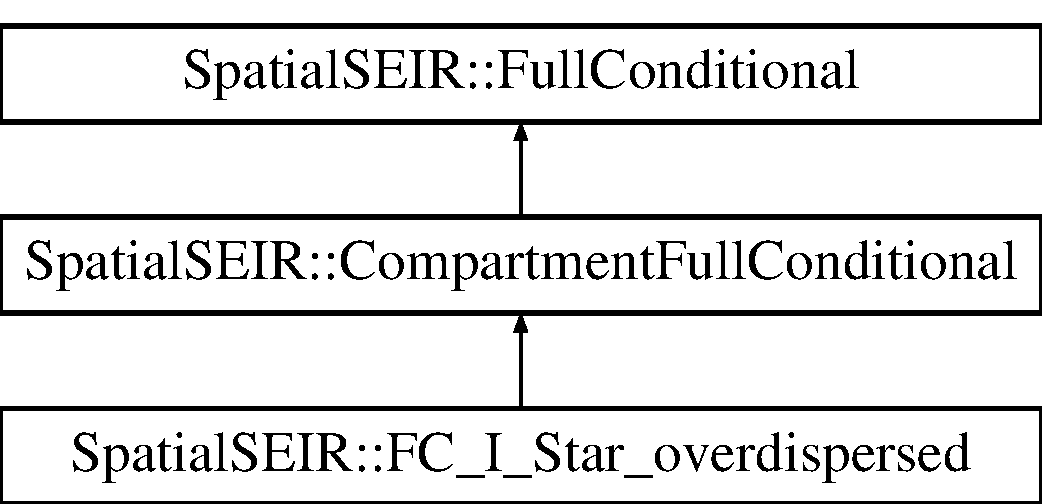
\includegraphics[height=3.000000cm]{classSpatialSEIR_1_1FC__I__Star__overdispersed}
\end{center}
\end{figure}
\subsection*{Public Member Functions}
\begin{DoxyCompactItemize}
\item 
\hyperlink{classSpatialSEIR_1_1FC__I__Star__overdispersed_ae01b90d643d41a1d040267154548cfbf}{F\-C\-\_\-\-I\-\_\-\-Star\-\_\-overdispersed} (\hyperlink{classSpatialSEIR_1_1ModelContext}{Model\-Context} $\ast$\-\_\-context, int $\ast$\-\_\-\-Y, \hyperlink{classSpatialSEIR_1_1CompartmentalModelMatrix}{Compartmental\-Model\-Matrix} $\ast$\-\_\-\-I\-\_\-star, \hyperlink{classSpatialSEIR_1_1CompartmentalModelMatrix}{Compartmental\-Model\-Matrix} $\ast$\-\_\-\-I, \hyperlink{classSpatialSEIR_1_1CompartmentalModelMatrix}{Compartmental\-Model\-Matrix} $\ast$\-\_\-\-E, \hyperlink{classSpatialSEIR_1_1CompartmentalModelMatrix}{Compartmental\-Model\-Matrix} $\ast$\-\_\-\-R\-\_\-star, double $\ast$\-\_\-p\-\_\-ei, double $\ast$\-\_\-p\-\_\-ir, double $\ast$\-\_\-phi, double \-\_\-steady\-State\-Constraint\-Precision, double \-\_\-slice\-Width)
\item 
virtual int \hyperlink{classSpatialSEIR_1_1FC__I__Star__overdispersed_ab9913de9f59f6a614b9a70d6d055b148}{eval\-C\-P\-U} ()
\item 
virtual int \hyperlink{classSpatialSEIR_1_1FC__I__Star__overdispersed_a35e7e87cda4bb50626598a63b1161d67}{eval\-C\-P\-U} (int i, int j)
\item 
virtual int \hyperlink{classSpatialSEIR_1_1FC__I__Star__overdispersed_ab3205feb288d0a8ce383904f527277cf}{eval\-O\-C\-L} ()
\item 
virtual void \hyperlink{classSpatialSEIR_1_1FC__I__Star__overdispersed_a49ec8bf35ee3122bc58fb2dbcfa35fcd}{sample} (int verbose)
\item 
virtual long double \hyperlink{classSpatialSEIR_1_1FC__I__Star__overdispersed_afc7b8947a99bfcd0abeb551542e47886}{get\-Value} ()
\item 
virtual void \hyperlink{classSpatialSEIR_1_1FC__I__Star__overdispersed_aeac6fb5229f36bb9e0a9db24ff6bc100}{set\-Value} (long double val)
\item 
virtual int \hyperlink{classSpatialSEIR_1_1FC__I__Star__overdispersed_a8e7bf521bf8f001a00fab473c297553c}{calculate\-Relevant\-Compartments} ()
\item 
virtual int \hyperlink{classSpatialSEIR_1_1FC__I__Star__overdispersed_a7455ba1ac215f3d00d37ecb6d3508006}{calculate\-Relevant\-Compartments} (int i, int j)
\item 
virtual int \hyperlink{classSpatialSEIR_1_1FC__I__Star__overdispersed_a8effecefb91a8c16a1a7a99d42326bf5}{calculate\-Relevant\-Compartments\-\_\-\-O\-C\-L} ()
\item 
virtual \hyperlink{classSpatialSEIR_1_1FC__I__Star__overdispersed_ab10730f38210464c51e5ed99460b8aac}{$\sim$\-F\-C\-\_\-\-I\-\_\-\-Star\-\_\-overdispersed} ()
\end{DoxyCompactItemize}
\subsection*{Public Attributes}
\begin{DoxyCompactItemize}
\item 
\hyperlink{classSpatialSEIR_1_1ModelContext}{Model\-Context} $\ast$$\ast$ \hyperlink{classSpatialSEIR_1_1FC__I__Star__overdispersed_ad900ca243647ff1a0aad4cbddf09d526}{context}
\item 
int $\ast$$\ast$ \hyperlink{classSpatialSEIR_1_1FC__I__Star__overdispersed_ade65d87298fcc402c6ac460aef295180}{Y}
\item 
\hyperlink{classSpatialSEIR_1_1CompartmentalModelMatrix}{Compartmental\-Model\-Matrix} $\ast$$\ast$ \hyperlink{classSpatialSEIR_1_1FC__I__Star__overdispersed_ad4744526a8882ecbbd7aa2e5dbaea96c}{I\-\_\-star}
\item 
\hyperlink{classSpatialSEIR_1_1CompartmentalModelMatrix}{Compartmental\-Model\-Matrix} $\ast$$\ast$ \hyperlink{classSpatialSEIR_1_1FC__I__Star__overdispersed_acfa3e76171de9ada554843ce43bb353f}{I}
\item 
\hyperlink{classSpatialSEIR_1_1CompartmentalModelMatrix}{Compartmental\-Model\-Matrix} $\ast$$\ast$ \hyperlink{classSpatialSEIR_1_1FC__I__Star__overdispersed_af797f5c00660e0c3f96563ac8e25160e}{E}
\item 
\hyperlink{classSpatialSEIR_1_1CompartmentalModelMatrix}{Compartmental\-Model\-Matrix} $\ast$$\ast$ \hyperlink{classSpatialSEIR_1_1FC__I__Star__overdispersed_a4459a1e540b6980737d36c4e9425862b}{R\-\_\-star}
\item 
\hyperlink{classSpatialSEIR_1_1InitData}{Init\-Data} $\ast$$\ast$ \hyperlink{classSpatialSEIR_1_1FC__I__Star__overdispersed_a2076d3cbc52d91182d2e659fc7668101}{A0}
\item 
double $\ast$$\ast$ \hyperlink{classSpatialSEIR_1_1FC__I__Star__overdispersed_aa7235e850643e3f73cfe5e941add3999}{p\-\_\-ei}
\item 
double $\ast$$\ast$ \hyperlink{classSpatialSEIR_1_1FC__I__Star__overdispersed_a02722ae119baaed1d50795af36c78aa5}{p\-\_\-ir}
\item 
double $\ast$$\ast$ \hyperlink{classSpatialSEIR_1_1FC__I__Star__overdispersed_a128a90fee53566ef1e093b2227f87814}{phi}
\item 
long double $\ast$ \hyperlink{classSpatialSEIR_1_1FC__I__Star__overdispersed_abc747c69c47f8b6019e27c64c0ddeb8c}{value}
\item 
double $\ast$ \hyperlink{classSpatialSEIR_1_1FC__I__Star__overdispersed_a32ef601f1c6b7c0131261f1eb0214e6d}{steady\-State\-Constraint\-Precision}
\end{DoxyCompactItemize}


\subsection{Detailed Description}
\hyperlink{classSpatialSEIR_1_1FC__I__Star__overdispersed}{F\-C\-\_\-\-I\-\_\-\-Star\-\_\-overdispersed} gives the overdispersion data model for I\-\_\-star. 

\subsection{Constructor \& Destructor Documentation}
\hypertarget{classSpatialSEIR_1_1FC__I__Star__overdispersed_ae01b90d643d41a1d040267154548cfbf}{\index{Spatial\-S\-E\-I\-R\-::\-F\-C\-\_\-\-I\-\_\-\-Star\-\_\-overdispersed@{Spatial\-S\-E\-I\-R\-::\-F\-C\-\_\-\-I\-\_\-\-Star\-\_\-overdispersed}!F\-C\-\_\-\-I\-\_\-\-Star\-\_\-overdispersed@{F\-C\-\_\-\-I\-\_\-\-Star\-\_\-overdispersed}}
\index{F\-C\-\_\-\-I\-\_\-\-Star\-\_\-overdispersed@{F\-C\-\_\-\-I\-\_\-\-Star\-\_\-overdispersed}!SpatialSEIR::FC_I_Star_overdispersed@{Spatial\-S\-E\-I\-R\-::\-F\-C\-\_\-\-I\-\_\-\-Star\-\_\-overdispersed}}
\subsubsection[{F\-C\-\_\-\-I\-\_\-\-Star\-\_\-overdispersed}]{\setlength{\rightskip}{0pt plus 5cm}Spatial\-S\-E\-I\-R\-::\-F\-C\-\_\-\-I\-\_\-\-Star\-\_\-overdispersed\-::\-F\-C\-\_\-\-I\-\_\-\-Star\-\_\-overdispersed (
\begin{DoxyParamCaption}
\item[{{\bf Model\-Context} $\ast$}]{\-\_\-context, }
\item[{int $\ast$}]{\-\_\-\-Y, }
\item[{{\bf Compartmental\-Model\-Matrix} $\ast$}]{\-\_\-\-I\-\_\-star, }
\item[{{\bf Compartmental\-Model\-Matrix} $\ast$}]{\-\_\-\-I, }
\item[{{\bf Compartmental\-Model\-Matrix} $\ast$}]{\-\_\-\-E, }
\item[{{\bf Compartmental\-Model\-Matrix} $\ast$}]{\-\_\-\-R\-\_\-star, }
\item[{double $\ast$}]{\-\_\-p\-\_\-ei, }
\item[{double $\ast$}]{\-\_\-p\-\_\-ir, }
\item[{double $\ast$}]{\-\_\-phi, }
\item[{double}]{\-\_\-steady\-State\-Constraint\-Precision, }
\item[{double}]{\-\_\-slice\-Width}
\end{DoxyParamCaption}
)}}\label{classSpatialSEIR_1_1FC__I__Star__overdispersed_ae01b90d643d41a1d040267154548cfbf}
\hypertarget{classSpatialSEIR_1_1FC__I__Star__overdispersed_ab10730f38210464c51e5ed99460b8aac}{\index{Spatial\-S\-E\-I\-R\-::\-F\-C\-\_\-\-I\-\_\-\-Star\-\_\-overdispersed@{Spatial\-S\-E\-I\-R\-::\-F\-C\-\_\-\-I\-\_\-\-Star\-\_\-overdispersed}!$\sim$\-F\-C\-\_\-\-I\-\_\-\-Star\-\_\-overdispersed@{$\sim$\-F\-C\-\_\-\-I\-\_\-\-Star\-\_\-overdispersed}}
\index{$\sim$\-F\-C\-\_\-\-I\-\_\-\-Star\-\_\-overdispersed@{$\sim$\-F\-C\-\_\-\-I\-\_\-\-Star\-\_\-overdispersed}!SpatialSEIR::FC_I_Star_overdispersed@{Spatial\-S\-E\-I\-R\-::\-F\-C\-\_\-\-I\-\_\-\-Star\-\_\-overdispersed}}
\subsubsection[{$\sim$\-F\-C\-\_\-\-I\-\_\-\-Star\-\_\-overdispersed}]{\setlength{\rightskip}{0pt plus 5cm}virtual Spatial\-S\-E\-I\-R\-::\-F\-C\-\_\-\-I\-\_\-\-Star\-\_\-overdispersed\-::$\sim$\-F\-C\-\_\-\-I\-\_\-\-Star\-\_\-overdispersed (
\begin{DoxyParamCaption}
{}
\end{DoxyParamCaption}
)\hspace{0.3cm}{\ttfamily [virtual]}}}\label{classSpatialSEIR_1_1FC__I__Star__overdispersed_ab10730f38210464c51e5ed99460b8aac}


\subsection{Member Function Documentation}
\hypertarget{classSpatialSEIR_1_1FC__I__Star__overdispersed_a8e7bf521bf8f001a00fab473c297553c}{\index{Spatial\-S\-E\-I\-R\-::\-F\-C\-\_\-\-I\-\_\-\-Star\-\_\-overdispersed@{Spatial\-S\-E\-I\-R\-::\-F\-C\-\_\-\-I\-\_\-\-Star\-\_\-overdispersed}!calculate\-Relevant\-Compartments@{calculate\-Relevant\-Compartments}}
\index{calculate\-Relevant\-Compartments@{calculate\-Relevant\-Compartments}!SpatialSEIR::FC_I_Star_overdispersed@{Spatial\-S\-E\-I\-R\-::\-F\-C\-\_\-\-I\-\_\-\-Star\-\_\-overdispersed}}
\subsubsection[{calculate\-Relevant\-Compartments}]{\setlength{\rightskip}{0pt plus 5cm}virtual int Spatial\-S\-E\-I\-R\-::\-F\-C\-\_\-\-I\-\_\-\-Star\-\_\-overdispersed\-::calculate\-Relevant\-Compartments (
\begin{DoxyParamCaption}
{}
\end{DoxyParamCaption}
)\hspace{0.3cm}{\ttfamily [virtual]}}}\label{classSpatialSEIR_1_1FC__I__Star__overdispersed_a8e7bf521bf8f001a00fab473c297553c}


Implements \hyperlink{classSpatialSEIR_1_1CompartmentFullConditional_a71836271b0997117f3b8437c2f55a986}{Spatial\-S\-E\-I\-R\-::\-Compartment\-Full\-Conditional}.

\hypertarget{classSpatialSEIR_1_1FC__I__Star__overdispersed_a7455ba1ac215f3d00d37ecb6d3508006}{\index{Spatial\-S\-E\-I\-R\-::\-F\-C\-\_\-\-I\-\_\-\-Star\-\_\-overdispersed@{Spatial\-S\-E\-I\-R\-::\-F\-C\-\_\-\-I\-\_\-\-Star\-\_\-overdispersed}!calculate\-Relevant\-Compartments@{calculate\-Relevant\-Compartments}}
\index{calculate\-Relevant\-Compartments@{calculate\-Relevant\-Compartments}!SpatialSEIR::FC_I_Star_overdispersed@{Spatial\-S\-E\-I\-R\-::\-F\-C\-\_\-\-I\-\_\-\-Star\-\_\-overdispersed}}
\subsubsection[{calculate\-Relevant\-Compartments}]{\setlength{\rightskip}{0pt plus 5cm}virtual int Spatial\-S\-E\-I\-R\-::\-F\-C\-\_\-\-I\-\_\-\-Star\-\_\-overdispersed\-::calculate\-Relevant\-Compartments (
\begin{DoxyParamCaption}
\item[{int}]{i, }
\item[{int}]{j}
\end{DoxyParamCaption}
)\hspace{0.3cm}{\ttfamily [virtual]}}}\label{classSpatialSEIR_1_1FC__I__Star__overdispersed_a7455ba1ac215f3d00d37ecb6d3508006}


Implements \hyperlink{classSpatialSEIR_1_1CompartmentFullConditional_a21440bf07bd554a2893a328713bfe09f}{Spatial\-S\-E\-I\-R\-::\-Compartment\-Full\-Conditional}.

\hypertarget{classSpatialSEIR_1_1FC__I__Star__overdispersed_a8effecefb91a8c16a1a7a99d42326bf5}{\index{Spatial\-S\-E\-I\-R\-::\-F\-C\-\_\-\-I\-\_\-\-Star\-\_\-overdispersed@{Spatial\-S\-E\-I\-R\-::\-F\-C\-\_\-\-I\-\_\-\-Star\-\_\-overdispersed}!calculate\-Relevant\-Compartments\-\_\-\-O\-C\-L@{calculate\-Relevant\-Compartments\-\_\-\-O\-C\-L}}
\index{calculate\-Relevant\-Compartments\-\_\-\-O\-C\-L@{calculate\-Relevant\-Compartments\-\_\-\-O\-C\-L}!SpatialSEIR::FC_I_Star_overdispersed@{Spatial\-S\-E\-I\-R\-::\-F\-C\-\_\-\-I\-\_\-\-Star\-\_\-overdispersed}}
\subsubsection[{calculate\-Relevant\-Compartments\-\_\-\-O\-C\-L}]{\setlength{\rightskip}{0pt plus 5cm}virtual int Spatial\-S\-E\-I\-R\-::\-F\-C\-\_\-\-I\-\_\-\-Star\-\_\-overdispersed\-::calculate\-Relevant\-Compartments\-\_\-\-O\-C\-L (
\begin{DoxyParamCaption}
{}
\end{DoxyParamCaption}
)\hspace{0.3cm}{\ttfamily [virtual]}}}\label{classSpatialSEIR_1_1FC__I__Star__overdispersed_a8effecefb91a8c16a1a7a99d42326bf5}


Implements \hyperlink{classSpatialSEIR_1_1CompartmentFullConditional_ab873ecc59f7639637113d885ab89bed4}{Spatial\-S\-E\-I\-R\-::\-Compartment\-Full\-Conditional}.

\hypertarget{classSpatialSEIR_1_1FC__I__Star__overdispersed_ab9913de9f59f6a614b9a70d6d055b148}{\index{Spatial\-S\-E\-I\-R\-::\-F\-C\-\_\-\-I\-\_\-\-Star\-\_\-overdispersed@{Spatial\-S\-E\-I\-R\-::\-F\-C\-\_\-\-I\-\_\-\-Star\-\_\-overdispersed}!eval\-C\-P\-U@{eval\-C\-P\-U}}
\index{eval\-C\-P\-U@{eval\-C\-P\-U}!SpatialSEIR::FC_I_Star_overdispersed@{Spatial\-S\-E\-I\-R\-::\-F\-C\-\_\-\-I\-\_\-\-Star\-\_\-overdispersed}}
\subsubsection[{eval\-C\-P\-U}]{\setlength{\rightskip}{0pt plus 5cm}virtual int Spatial\-S\-E\-I\-R\-::\-F\-C\-\_\-\-I\-\_\-\-Star\-\_\-overdispersed\-::eval\-C\-P\-U (
\begin{DoxyParamCaption}
{}
\end{DoxyParamCaption}
)\hspace{0.3cm}{\ttfamily [virtual]}}}\label{classSpatialSEIR_1_1FC__I__Star__overdispersed_ab9913de9f59f6a614b9a70d6d055b148}


Implements \hyperlink{classSpatialSEIR_1_1CompartmentFullConditional_ad2402c8d7fc0b362482bcd5ceaa035af}{Spatial\-S\-E\-I\-R\-::\-Compartment\-Full\-Conditional}.

\hypertarget{classSpatialSEIR_1_1FC__I__Star__overdispersed_a35e7e87cda4bb50626598a63b1161d67}{\index{Spatial\-S\-E\-I\-R\-::\-F\-C\-\_\-\-I\-\_\-\-Star\-\_\-overdispersed@{Spatial\-S\-E\-I\-R\-::\-F\-C\-\_\-\-I\-\_\-\-Star\-\_\-overdispersed}!eval\-C\-P\-U@{eval\-C\-P\-U}}
\index{eval\-C\-P\-U@{eval\-C\-P\-U}!SpatialSEIR::FC_I_Star_overdispersed@{Spatial\-S\-E\-I\-R\-::\-F\-C\-\_\-\-I\-\_\-\-Star\-\_\-overdispersed}}
\subsubsection[{eval\-C\-P\-U}]{\setlength{\rightskip}{0pt plus 5cm}virtual int Spatial\-S\-E\-I\-R\-::\-F\-C\-\_\-\-I\-\_\-\-Star\-\_\-overdispersed\-::eval\-C\-P\-U (
\begin{DoxyParamCaption}
\item[{int}]{i, }
\item[{int}]{j}
\end{DoxyParamCaption}
)\hspace{0.3cm}{\ttfamily [virtual]}}}\label{classSpatialSEIR_1_1FC__I__Star__overdispersed_a35e7e87cda4bb50626598a63b1161d67}


Implements \hyperlink{classSpatialSEIR_1_1CompartmentFullConditional_a92d48bc8cd13ff048791edbdcc453479}{Spatial\-S\-E\-I\-R\-::\-Compartment\-Full\-Conditional}.

\hypertarget{classSpatialSEIR_1_1FC__I__Star__overdispersed_ab3205feb288d0a8ce383904f527277cf}{\index{Spatial\-S\-E\-I\-R\-::\-F\-C\-\_\-\-I\-\_\-\-Star\-\_\-overdispersed@{Spatial\-S\-E\-I\-R\-::\-F\-C\-\_\-\-I\-\_\-\-Star\-\_\-overdispersed}!eval\-O\-C\-L@{eval\-O\-C\-L}}
\index{eval\-O\-C\-L@{eval\-O\-C\-L}!SpatialSEIR::FC_I_Star_overdispersed@{Spatial\-S\-E\-I\-R\-::\-F\-C\-\_\-\-I\-\_\-\-Star\-\_\-overdispersed}}
\subsubsection[{eval\-O\-C\-L}]{\setlength{\rightskip}{0pt plus 5cm}virtual int Spatial\-S\-E\-I\-R\-::\-F\-C\-\_\-\-I\-\_\-\-Star\-\_\-overdispersed\-::eval\-O\-C\-L (
\begin{DoxyParamCaption}
{}
\end{DoxyParamCaption}
)\hspace{0.3cm}{\ttfamily [virtual]}}}\label{classSpatialSEIR_1_1FC__I__Star__overdispersed_ab3205feb288d0a8ce383904f527277cf}


Implements \hyperlink{classSpatialSEIR_1_1CompartmentFullConditional_ac7c7b1191508d49a56ec739449bf93d4}{Spatial\-S\-E\-I\-R\-::\-Compartment\-Full\-Conditional}.

\hypertarget{classSpatialSEIR_1_1FC__I__Star__overdispersed_afc7b8947a99bfcd0abeb551542e47886}{\index{Spatial\-S\-E\-I\-R\-::\-F\-C\-\_\-\-I\-\_\-\-Star\-\_\-overdispersed@{Spatial\-S\-E\-I\-R\-::\-F\-C\-\_\-\-I\-\_\-\-Star\-\_\-overdispersed}!get\-Value@{get\-Value}}
\index{get\-Value@{get\-Value}!SpatialSEIR::FC_I_Star_overdispersed@{Spatial\-S\-E\-I\-R\-::\-F\-C\-\_\-\-I\-\_\-\-Star\-\_\-overdispersed}}
\subsubsection[{get\-Value}]{\setlength{\rightskip}{0pt plus 5cm}virtual long double Spatial\-S\-E\-I\-R\-::\-F\-C\-\_\-\-I\-\_\-\-Star\-\_\-overdispersed\-::get\-Value (
\begin{DoxyParamCaption}
{}
\end{DoxyParamCaption}
)\hspace{0.3cm}{\ttfamily [virtual]}}}\label{classSpatialSEIR_1_1FC__I__Star__overdispersed_afc7b8947a99bfcd0abeb551542e47886}


Implements \hyperlink{classSpatialSEIR_1_1CompartmentFullConditional_a28794be23ee7f6fcba96ff2bee63e065}{Spatial\-S\-E\-I\-R\-::\-Compartment\-Full\-Conditional}.

\hypertarget{classSpatialSEIR_1_1FC__I__Star__overdispersed_a49ec8bf35ee3122bc58fb2dbcfa35fcd}{\index{Spatial\-S\-E\-I\-R\-::\-F\-C\-\_\-\-I\-\_\-\-Star\-\_\-overdispersed@{Spatial\-S\-E\-I\-R\-::\-F\-C\-\_\-\-I\-\_\-\-Star\-\_\-overdispersed}!sample@{sample}}
\index{sample@{sample}!SpatialSEIR::FC_I_Star_overdispersed@{Spatial\-S\-E\-I\-R\-::\-F\-C\-\_\-\-I\-\_\-\-Star\-\_\-overdispersed}}
\subsubsection[{sample}]{\setlength{\rightskip}{0pt plus 5cm}virtual void Spatial\-S\-E\-I\-R\-::\-F\-C\-\_\-\-I\-\_\-\-Star\-\_\-overdispersed\-::sample (
\begin{DoxyParamCaption}
\item[{int}]{verbose}
\end{DoxyParamCaption}
)\hspace{0.3cm}{\ttfamily [virtual]}}}\label{classSpatialSEIR_1_1FC__I__Star__overdispersed_a49ec8bf35ee3122bc58fb2dbcfa35fcd}


Implements \hyperlink{classSpatialSEIR_1_1CompartmentFullConditional_a436ae9e47f7a4269f0a78ce225e6b7f3}{Spatial\-S\-E\-I\-R\-::\-Compartment\-Full\-Conditional}.

\hypertarget{classSpatialSEIR_1_1FC__I__Star__overdispersed_aeac6fb5229f36bb9e0a9db24ff6bc100}{\index{Spatial\-S\-E\-I\-R\-::\-F\-C\-\_\-\-I\-\_\-\-Star\-\_\-overdispersed@{Spatial\-S\-E\-I\-R\-::\-F\-C\-\_\-\-I\-\_\-\-Star\-\_\-overdispersed}!set\-Value@{set\-Value}}
\index{set\-Value@{set\-Value}!SpatialSEIR::FC_I_Star_overdispersed@{Spatial\-S\-E\-I\-R\-::\-F\-C\-\_\-\-I\-\_\-\-Star\-\_\-overdispersed}}
\subsubsection[{set\-Value}]{\setlength{\rightskip}{0pt plus 5cm}virtual void Spatial\-S\-E\-I\-R\-::\-F\-C\-\_\-\-I\-\_\-\-Star\-\_\-overdispersed\-::set\-Value (
\begin{DoxyParamCaption}
\item[{long double}]{val}
\end{DoxyParamCaption}
)\hspace{0.3cm}{\ttfamily [virtual]}}}\label{classSpatialSEIR_1_1FC__I__Star__overdispersed_aeac6fb5229f36bb9e0a9db24ff6bc100}


Implements \hyperlink{classSpatialSEIR_1_1CompartmentFullConditional_a22ab4dcc354c8ebc4f619685bc32dfae}{Spatial\-S\-E\-I\-R\-::\-Compartment\-Full\-Conditional}.



\subsection{Member Data Documentation}
\hypertarget{classSpatialSEIR_1_1FC__I__Star__overdispersed_a2076d3cbc52d91182d2e659fc7668101}{\index{Spatial\-S\-E\-I\-R\-::\-F\-C\-\_\-\-I\-\_\-\-Star\-\_\-overdispersed@{Spatial\-S\-E\-I\-R\-::\-F\-C\-\_\-\-I\-\_\-\-Star\-\_\-overdispersed}!A0@{A0}}
\index{A0@{A0}!SpatialSEIR::FC_I_Star_overdispersed@{Spatial\-S\-E\-I\-R\-::\-F\-C\-\_\-\-I\-\_\-\-Star\-\_\-overdispersed}}
\subsubsection[{A0}]{\setlength{\rightskip}{0pt plus 5cm}{\bf Init\-Data}$\ast$$\ast$ Spatial\-S\-E\-I\-R\-::\-F\-C\-\_\-\-I\-\_\-\-Star\-\_\-overdispersed\-::\-A0}}\label{classSpatialSEIR_1_1FC__I__Star__overdispersed_a2076d3cbc52d91182d2e659fc7668101}
\hypertarget{classSpatialSEIR_1_1FC__I__Star__overdispersed_ad900ca243647ff1a0aad4cbddf09d526}{\index{Spatial\-S\-E\-I\-R\-::\-F\-C\-\_\-\-I\-\_\-\-Star\-\_\-overdispersed@{Spatial\-S\-E\-I\-R\-::\-F\-C\-\_\-\-I\-\_\-\-Star\-\_\-overdispersed}!context@{context}}
\index{context@{context}!SpatialSEIR::FC_I_Star_overdispersed@{Spatial\-S\-E\-I\-R\-::\-F\-C\-\_\-\-I\-\_\-\-Star\-\_\-overdispersed}}
\subsubsection[{context}]{\setlength{\rightskip}{0pt plus 5cm}{\bf Model\-Context}$\ast$$\ast$ Spatial\-S\-E\-I\-R\-::\-F\-C\-\_\-\-I\-\_\-\-Star\-\_\-overdispersed\-::context}}\label{classSpatialSEIR_1_1FC__I__Star__overdispersed_ad900ca243647ff1a0aad4cbddf09d526}
\hypertarget{classSpatialSEIR_1_1FC__I__Star__overdispersed_af797f5c00660e0c3f96563ac8e25160e}{\index{Spatial\-S\-E\-I\-R\-::\-F\-C\-\_\-\-I\-\_\-\-Star\-\_\-overdispersed@{Spatial\-S\-E\-I\-R\-::\-F\-C\-\_\-\-I\-\_\-\-Star\-\_\-overdispersed}!E@{E}}
\index{E@{E}!SpatialSEIR::FC_I_Star_overdispersed@{Spatial\-S\-E\-I\-R\-::\-F\-C\-\_\-\-I\-\_\-\-Star\-\_\-overdispersed}}
\subsubsection[{E}]{\setlength{\rightskip}{0pt plus 5cm}{\bf Compartmental\-Model\-Matrix}$\ast$$\ast$ Spatial\-S\-E\-I\-R\-::\-F\-C\-\_\-\-I\-\_\-\-Star\-\_\-overdispersed\-::\-E}}\label{classSpatialSEIR_1_1FC__I__Star__overdispersed_af797f5c00660e0c3f96563ac8e25160e}
\hypertarget{classSpatialSEIR_1_1FC__I__Star__overdispersed_acfa3e76171de9ada554843ce43bb353f}{\index{Spatial\-S\-E\-I\-R\-::\-F\-C\-\_\-\-I\-\_\-\-Star\-\_\-overdispersed@{Spatial\-S\-E\-I\-R\-::\-F\-C\-\_\-\-I\-\_\-\-Star\-\_\-overdispersed}!I@{I}}
\index{I@{I}!SpatialSEIR::FC_I_Star_overdispersed@{Spatial\-S\-E\-I\-R\-::\-F\-C\-\_\-\-I\-\_\-\-Star\-\_\-overdispersed}}
\subsubsection[{I}]{\setlength{\rightskip}{0pt plus 5cm}{\bf Compartmental\-Model\-Matrix}$\ast$$\ast$ Spatial\-S\-E\-I\-R\-::\-F\-C\-\_\-\-I\-\_\-\-Star\-\_\-overdispersed\-::\-I}}\label{classSpatialSEIR_1_1FC__I__Star__overdispersed_acfa3e76171de9ada554843ce43bb353f}
\hypertarget{classSpatialSEIR_1_1FC__I__Star__overdispersed_ad4744526a8882ecbbd7aa2e5dbaea96c}{\index{Spatial\-S\-E\-I\-R\-::\-F\-C\-\_\-\-I\-\_\-\-Star\-\_\-overdispersed@{Spatial\-S\-E\-I\-R\-::\-F\-C\-\_\-\-I\-\_\-\-Star\-\_\-overdispersed}!I\-\_\-star@{I\-\_\-star}}
\index{I\-\_\-star@{I\-\_\-star}!SpatialSEIR::FC_I_Star_overdispersed@{Spatial\-S\-E\-I\-R\-::\-F\-C\-\_\-\-I\-\_\-\-Star\-\_\-overdispersed}}
\subsubsection[{I\-\_\-star}]{\setlength{\rightskip}{0pt plus 5cm}{\bf Compartmental\-Model\-Matrix}$\ast$$\ast$ Spatial\-S\-E\-I\-R\-::\-F\-C\-\_\-\-I\-\_\-\-Star\-\_\-overdispersed\-::\-I\-\_\-star}}\label{classSpatialSEIR_1_1FC__I__Star__overdispersed_ad4744526a8882ecbbd7aa2e5dbaea96c}
\hypertarget{classSpatialSEIR_1_1FC__I__Star__overdispersed_aa7235e850643e3f73cfe5e941add3999}{\index{Spatial\-S\-E\-I\-R\-::\-F\-C\-\_\-\-I\-\_\-\-Star\-\_\-overdispersed@{Spatial\-S\-E\-I\-R\-::\-F\-C\-\_\-\-I\-\_\-\-Star\-\_\-overdispersed}!p\-\_\-ei@{p\-\_\-ei}}
\index{p\-\_\-ei@{p\-\_\-ei}!SpatialSEIR::FC_I_Star_overdispersed@{Spatial\-S\-E\-I\-R\-::\-F\-C\-\_\-\-I\-\_\-\-Star\-\_\-overdispersed}}
\subsubsection[{p\-\_\-ei}]{\setlength{\rightskip}{0pt plus 5cm}double$\ast$$\ast$ Spatial\-S\-E\-I\-R\-::\-F\-C\-\_\-\-I\-\_\-\-Star\-\_\-overdispersed\-::p\-\_\-ei}}\label{classSpatialSEIR_1_1FC__I__Star__overdispersed_aa7235e850643e3f73cfe5e941add3999}
\hypertarget{classSpatialSEIR_1_1FC__I__Star__overdispersed_a02722ae119baaed1d50795af36c78aa5}{\index{Spatial\-S\-E\-I\-R\-::\-F\-C\-\_\-\-I\-\_\-\-Star\-\_\-overdispersed@{Spatial\-S\-E\-I\-R\-::\-F\-C\-\_\-\-I\-\_\-\-Star\-\_\-overdispersed}!p\-\_\-ir@{p\-\_\-ir}}
\index{p\-\_\-ir@{p\-\_\-ir}!SpatialSEIR::FC_I_Star_overdispersed@{Spatial\-S\-E\-I\-R\-::\-F\-C\-\_\-\-I\-\_\-\-Star\-\_\-overdispersed}}
\subsubsection[{p\-\_\-ir}]{\setlength{\rightskip}{0pt plus 5cm}double$\ast$$\ast$ Spatial\-S\-E\-I\-R\-::\-F\-C\-\_\-\-I\-\_\-\-Star\-\_\-overdispersed\-::p\-\_\-ir}}\label{classSpatialSEIR_1_1FC__I__Star__overdispersed_a02722ae119baaed1d50795af36c78aa5}
\hypertarget{classSpatialSEIR_1_1FC__I__Star__overdispersed_a128a90fee53566ef1e093b2227f87814}{\index{Spatial\-S\-E\-I\-R\-::\-F\-C\-\_\-\-I\-\_\-\-Star\-\_\-overdispersed@{Spatial\-S\-E\-I\-R\-::\-F\-C\-\_\-\-I\-\_\-\-Star\-\_\-overdispersed}!phi@{phi}}
\index{phi@{phi}!SpatialSEIR::FC_I_Star_overdispersed@{Spatial\-S\-E\-I\-R\-::\-F\-C\-\_\-\-I\-\_\-\-Star\-\_\-overdispersed}}
\subsubsection[{phi}]{\setlength{\rightskip}{0pt plus 5cm}double$\ast$$\ast$ Spatial\-S\-E\-I\-R\-::\-F\-C\-\_\-\-I\-\_\-\-Star\-\_\-overdispersed\-::phi}}\label{classSpatialSEIR_1_1FC__I__Star__overdispersed_a128a90fee53566ef1e093b2227f87814}
\hypertarget{classSpatialSEIR_1_1FC__I__Star__overdispersed_a4459a1e540b6980737d36c4e9425862b}{\index{Spatial\-S\-E\-I\-R\-::\-F\-C\-\_\-\-I\-\_\-\-Star\-\_\-overdispersed@{Spatial\-S\-E\-I\-R\-::\-F\-C\-\_\-\-I\-\_\-\-Star\-\_\-overdispersed}!R\-\_\-star@{R\-\_\-star}}
\index{R\-\_\-star@{R\-\_\-star}!SpatialSEIR::FC_I_Star_overdispersed@{Spatial\-S\-E\-I\-R\-::\-F\-C\-\_\-\-I\-\_\-\-Star\-\_\-overdispersed}}
\subsubsection[{R\-\_\-star}]{\setlength{\rightskip}{0pt plus 5cm}{\bf Compartmental\-Model\-Matrix}$\ast$$\ast$ Spatial\-S\-E\-I\-R\-::\-F\-C\-\_\-\-I\-\_\-\-Star\-\_\-overdispersed\-::\-R\-\_\-star}}\label{classSpatialSEIR_1_1FC__I__Star__overdispersed_a4459a1e540b6980737d36c4e9425862b}
\hypertarget{classSpatialSEIR_1_1FC__I__Star__overdispersed_a32ef601f1c6b7c0131261f1eb0214e6d}{\index{Spatial\-S\-E\-I\-R\-::\-F\-C\-\_\-\-I\-\_\-\-Star\-\_\-overdispersed@{Spatial\-S\-E\-I\-R\-::\-F\-C\-\_\-\-I\-\_\-\-Star\-\_\-overdispersed}!steady\-State\-Constraint\-Precision@{steady\-State\-Constraint\-Precision}}
\index{steady\-State\-Constraint\-Precision@{steady\-State\-Constraint\-Precision}!SpatialSEIR::FC_I_Star_overdispersed@{Spatial\-S\-E\-I\-R\-::\-F\-C\-\_\-\-I\-\_\-\-Star\-\_\-overdispersed}}
\subsubsection[{steady\-State\-Constraint\-Precision}]{\setlength{\rightskip}{0pt plus 5cm}double$\ast$ Spatial\-S\-E\-I\-R\-::\-F\-C\-\_\-\-I\-\_\-\-Star\-\_\-overdispersed\-::steady\-State\-Constraint\-Precision}}\label{classSpatialSEIR_1_1FC__I__Star__overdispersed_a32ef601f1c6b7c0131261f1eb0214e6d}
\hypertarget{classSpatialSEIR_1_1FC__I__Star__overdispersed_abc747c69c47f8b6019e27c64c0ddeb8c}{\index{Spatial\-S\-E\-I\-R\-::\-F\-C\-\_\-\-I\-\_\-\-Star\-\_\-overdispersed@{Spatial\-S\-E\-I\-R\-::\-F\-C\-\_\-\-I\-\_\-\-Star\-\_\-overdispersed}!value@{value}}
\index{value@{value}!SpatialSEIR::FC_I_Star_overdispersed@{Spatial\-S\-E\-I\-R\-::\-F\-C\-\_\-\-I\-\_\-\-Star\-\_\-overdispersed}}
\subsubsection[{value}]{\setlength{\rightskip}{0pt plus 5cm}long double$\ast$ Spatial\-S\-E\-I\-R\-::\-F\-C\-\_\-\-I\-\_\-\-Star\-\_\-overdispersed\-::value}}\label{classSpatialSEIR_1_1FC__I__Star__overdispersed_abc747c69c47f8b6019e27c64c0ddeb8c}
\hypertarget{classSpatialSEIR_1_1FC__I__Star__overdispersed_ade65d87298fcc402c6ac460aef295180}{\index{Spatial\-S\-E\-I\-R\-::\-F\-C\-\_\-\-I\-\_\-\-Star\-\_\-overdispersed@{Spatial\-S\-E\-I\-R\-::\-F\-C\-\_\-\-I\-\_\-\-Star\-\_\-overdispersed}!Y@{Y}}
\index{Y@{Y}!SpatialSEIR::FC_I_Star_overdispersed@{Spatial\-S\-E\-I\-R\-::\-F\-C\-\_\-\-I\-\_\-\-Star\-\_\-overdispersed}}
\subsubsection[{Y}]{\setlength{\rightskip}{0pt plus 5cm}int$\ast$$\ast$ Spatial\-S\-E\-I\-R\-::\-F\-C\-\_\-\-I\-\_\-\-Star\-\_\-overdispersed\-::\-Y}}\label{classSpatialSEIR_1_1FC__I__Star__overdispersed_ade65d87298fcc402c6ac460aef295180}


The documentation for this class was generated from the following file\-:\begin{DoxyCompactItemize}
\item 
lib\-Spatial\-S\-E\-I\-R/include/\-Full\-Conditionals/\-Data\-Models/\-Overdispersion/\hyperlink{LSS__FC__I__star__overdispersion_8hpp}{L\-S\-S\-\_\-\-F\-C\-\_\-\-I\-\_\-star\-\_\-overdispersion.\-hpp}\end{DoxyCompactItemize}

\hypertarget{classSpatialSEIR_1_1FC__Phi}{\section{Spatial\-S\-E\-I\-R\-:\-:F\-C\-\_\-\-Phi Class Reference}
\label{classSpatialSEIR_1_1FC__Phi}\index{Spatial\-S\-E\-I\-R\-::\-F\-C\-\_\-\-Phi@{Spatial\-S\-E\-I\-R\-::\-F\-C\-\_\-\-Phi}}
}


{\ttfamily \#include $<$L\-S\-S\-\_\-\-F\-C\-\_\-\-Phi.\-hpp$>$}

Inheritance diagram for Spatial\-S\-E\-I\-R\-:\-:F\-C\-\_\-\-Phi\-:\begin{figure}[H]
\begin{center}
\leavevmode
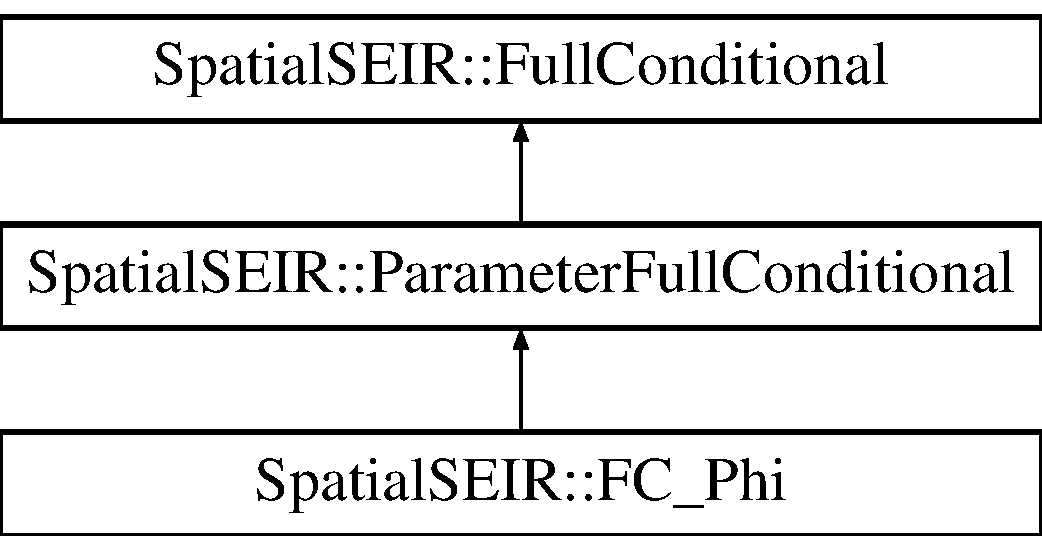
\includegraphics[height=3.000000cm]{classSpatialSEIR_1_1FC__Phi}
\end{center}
\end{figure}
\subsection*{Public Member Functions}
\begin{DoxyCompactItemize}
\item 
\hyperlink{classSpatialSEIR_1_1FC__Phi_afa42036238ea301db57410a08da92d8f}{F\-C\-\_\-\-Phi} (\hyperlink{classSpatialSEIR_1_1ModelContext}{Model\-Context} $\ast$\-\_\-context, \hyperlink{classSpatialSEIR_1_1CompartmentalModelMatrix}{Compartmental\-Model\-Matrix} $\ast$\-\_\-\-I\-\_\-star, double $\ast$\-\_\-phi, double \-\_\-prior\-Alpha, double \-\_\-prior\-Beta, int $\ast$\-\_\-\-Y, double \hyperlink{classSpatialSEIR_1_1FullConditional_a150ee031af8d086ad0a04b13630a110f}{slice\-Width})
\item 
\hyperlink{classSpatialSEIR_1_1FC__Phi_ab83a41edc6b119b0bf94105c929863ee}{$\sim$\-F\-C\-\_\-\-Phi} ()
\item 
virtual double \hyperlink{classSpatialSEIR_1_1FC__Phi_aa7773cd1f79ac2cc0aa0022b871be037}{eval\-Prior} ()
\item 
virtual int \hyperlink{classSpatialSEIR_1_1FC__Phi_a282b0c3778149a8f29364ff56543288d}{eval\-C\-P\-U} ()
\item 
virtual int \hyperlink{classSpatialSEIR_1_1FC__Phi_aa0683e5c52d7cfdaf106fe9d20348845}{eval\-O\-C\-L} ()
\item 
virtual void \hyperlink{classSpatialSEIR_1_1FC__Phi_ad01626131955f37c6abec78af34524dd}{sample} (int verbose)
\item 
virtual long double \hyperlink{classSpatialSEIR_1_1FC__Phi_a78d2ad18fd2696bdd91333b1b4d8984e}{get\-Value} ()
\item 
virtual void \hyperlink{classSpatialSEIR_1_1FC__Phi_a71c23b1ea81880634e867786569b8b26}{set\-Value} (long double val)
\item 
virtual int \hyperlink{classSpatialSEIR_1_1FC__Phi_a738d592a5efd1f6181b28b2f294d4f86}{calculate\-Relevant\-Compartments} ()
\item 
virtual int \hyperlink{classSpatialSEIR_1_1FC__Phi_acb391933ee8f5efd16d392b62d400933}{calculate\-Relevant\-Compartments\-\_\-\-O\-C\-L} ()
\end{DoxyCompactItemize}
\subsection*{Public Attributes}
\begin{DoxyCompactItemize}
\item 
\hyperlink{classSpatialSEIR_1_1ModelContext}{Model\-Context} $\ast$$\ast$ \hyperlink{classSpatialSEIR_1_1FC__Phi_ad6a811039932fb9d393950d51e2a66d5}{context}
\item 
\hyperlink{classSpatialSEIR_1_1CompartmentalModelMatrix}{Compartmental\-Model\-Matrix} $\ast$$\ast$ \hyperlink{classSpatialSEIR_1_1FC__Phi_a5b07b79b34c5c6e2c81748b4fd8c0961}{I\-\_\-star}
\item 
double $\ast$$\ast$ \hyperlink{classSpatialSEIR_1_1FC__Phi_a40287a4878b59620961c279a8cb31672}{phi}
\item 
double $\ast$ \hyperlink{classSpatialSEIR_1_1FC__Phi_a416262207b7dff48d89e16fd31d7a41f}{prior\-Alpha}
\item 
double $\ast$ \hyperlink{classSpatialSEIR_1_1FC__Phi_ad65cf8a1b9bc7fc76e63bfe6d051dda6}{prior\-Beta}
\item 
int $\ast$$\ast$ \hyperlink{classSpatialSEIR_1_1FC__Phi_a74748c40d5729ec9bdacbc04f2294548}{Y}
\item 
long double $\ast$ \hyperlink{classSpatialSEIR_1_1FC__Phi_a649b11fba5f8820f83ced5a538f40fa3}{value}
\end{DoxyCompactItemize}


\subsection{Detailed Description}
\hyperlink{classSpatialSEIR_1_1FC__Phi}{F\-C\-\_\-\-Phi} gives the full conditional distribution of rho, the scalar spatial dependence parameter. 

\subsection{Constructor \& Destructor Documentation}
\hypertarget{classSpatialSEIR_1_1FC__Phi_afa42036238ea301db57410a08da92d8f}{\index{Spatial\-S\-E\-I\-R\-::\-F\-C\-\_\-\-Phi@{Spatial\-S\-E\-I\-R\-::\-F\-C\-\_\-\-Phi}!F\-C\-\_\-\-Phi@{F\-C\-\_\-\-Phi}}
\index{F\-C\-\_\-\-Phi@{F\-C\-\_\-\-Phi}!SpatialSEIR::FC_Phi@{Spatial\-S\-E\-I\-R\-::\-F\-C\-\_\-\-Phi}}
\subsubsection[{F\-C\-\_\-\-Phi}]{\setlength{\rightskip}{0pt plus 5cm}Spatial\-S\-E\-I\-R\-::\-F\-C\-\_\-\-Phi\-::\-F\-C\-\_\-\-Phi (
\begin{DoxyParamCaption}
\item[{{\bf Model\-Context} $\ast$}]{\-\_\-context, }
\item[{{\bf Compartmental\-Model\-Matrix} $\ast$}]{\-\_\-\-I\-\_\-star, }
\item[{double $\ast$}]{\-\_\-phi, }
\item[{double}]{\-\_\-prior\-Alpha, }
\item[{double}]{\-\_\-prior\-Beta, }
\item[{int $\ast$}]{\-\_\-\-Y, }
\item[{double}]{slice\-Width}
\end{DoxyParamCaption}
)}}\label{classSpatialSEIR_1_1FC__Phi_afa42036238ea301db57410a08da92d8f}
\hypertarget{classSpatialSEIR_1_1FC__Phi_ab83a41edc6b119b0bf94105c929863ee}{\index{Spatial\-S\-E\-I\-R\-::\-F\-C\-\_\-\-Phi@{Spatial\-S\-E\-I\-R\-::\-F\-C\-\_\-\-Phi}!$\sim$\-F\-C\-\_\-\-Phi@{$\sim$\-F\-C\-\_\-\-Phi}}
\index{$\sim$\-F\-C\-\_\-\-Phi@{$\sim$\-F\-C\-\_\-\-Phi}!SpatialSEIR::FC_Phi@{Spatial\-S\-E\-I\-R\-::\-F\-C\-\_\-\-Phi}}
\subsubsection[{$\sim$\-F\-C\-\_\-\-Phi}]{\setlength{\rightskip}{0pt plus 5cm}Spatial\-S\-E\-I\-R\-::\-F\-C\-\_\-\-Phi\-::$\sim$\-F\-C\-\_\-\-Phi (
\begin{DoxyParamCaption}
{}
\end{DoxyParamCaption}
)}}\label{classSpatialSEIR_1_1FC__Phi_ab83a41edc6b119b0bf94105c929863ee}


\subsection{Member Function Documentation}
\hypertarget{classSpatialSEIR_1_1FC__Phi_a738d592a5efd1f6181b28b2f294d4f86}{\index{Spatial\-S\-E\-I\-R\-::\-F\-C\-\_\-\-Phi@{Spatial\-S\-E\-I\-R\-::\-F\-C\-\_\-\-Phi}!calculate\-Relevant\-Compartments@{calculate\-Relevant\-Compartments}}
\index{calculate\-Relevant\-Compartments@{calculate\-Relevant\-Compartments}!SpatialSEIR::FC_Phi@{Spatial\-S\-E\-I\-R\-::\-F\-C\-\_\-\-Phi}}
\subsubsection[{calculate\-Relevant\-Compartments}]{\setlength{\rightskip}{0pt plus 5cm}virtual int Spatial\-S\-E\-I\-R\-::\-F\-C\-\_\-\-Phi\-::calculate\-Relevant\-Compartments (
\begin{DoxyParamCaption}
{}
\end{DoxyParamCaption}
)\hspace{0.3cm}{\ttfamily [virtual]}}}\label{classSpatialSEIR_1_1FC__Phi_a738d592a5efd1f6181b28b2f294d4f86}


Implements \hyperlink{classSpatialSEIR_1_1ParameterFullConditional_a65c39a2c3ca56e2f194b78cd362d35f9}{Spatial\-S\-E\-I\-R\-::\-Parameter\-Full\-Conditional}.

\hypertarget{classSpatialSEIR_1_1FC__Phi_acb391933ee8f5efd16d392b62d400933}{\index{Spatial\-S\-E\-I\-R\-::\-F\-C\-\_\-\-Phi@{Spatial\-S\-E\-I\-R\-::\-F\-C\-\_\-\-Phi}!calculate\-Relevant\-Compartments\-\_\-\-O\-C\-L@{calculate\-Relevant\-Compartments\-\_\-\-O\-C\-L}}
\index{calculate\-Relevant\-Compartments\-\_\-\-O\-C\-L@{calculate\-Relevant\-Compartments\-\_\-\-O\-C\-L}!SpatialSEIR::FC_Phi@{Spatial\-S\-E\-I\-R\-::\-F\-C\-\_\-\-Phi}}
\subsubsection[{calculate\-Relevant\-Compartments\-\_\-\-O\-C\-L}]{\setlength{\rightskip}{0pt plus 5cm}virtual int Spatial\-S\-E\-I\-R\-::\-F\-C\-\_\-\-Phi\-::calculate\-Relevant\-Compartments\-\_\-\-O\-C\-L (
\begin{DoxyParamCaption}
{}
\end{DoxyParamCaption}
)\hspace{0.3cm}{\ttfamily [virtual]}}}\label{classSpatialSEIR_1_1FC__Phi_acb391933ee8f5efd16d392b62d400933}


Implements \hyperlink{classSpatialSEIR_1_1ParameterFullConditional_af40754537736a64f58848e0368b001fb}{Spatial\-S\-E\-I\-R\-::\-Parameter\-Full\-Conditional}.

\hypertarget{classSpatialSEIR_1_1FC__Phi_a282b0c3778149a8f29364ff56543288d}{\index{Spatial\-S\-E\-I\-R\-::\-F\-C\-\_\-\-Phi@{Spatial\-S\-E\-I\-R\-::\-F\-C\-\_\-\-Phi}!eval\-C\-P\-U@{eval\-C\-P\-U}}
\index{eval\-C\-P\-U@{eval\-C\-P\-U}!SpatialSEIR::FC_Phi@{Spatial\-S\-E\-I\-R\-::\-F\-C\-\_\-\-Phi}}
\subsubsection[{eval\-C\-P\-U}]{\setlength{\rightskip}{0pt plus 5cm}virtual int Spatial\-S\-E\-I\-R\-::\-F\-C\-\_\-\-Phi\-::eval\-C\-P\-U (
\begin{DoxyParamCaption}
{}
\end{DoxyParamCaption}
)\hspace{0.3cm}{\ttfamily [virtual]}}}\label{classSpatialSEIR_1_1FC__Phi_a282b0c3778149a8f29364ff56543288d}


Implements \hyperlink{classSpatialSEIR_1_1ParameterFullConditional_a186bd19fdeb52ca4522f56fb880201dd}{Spatial\-S\-E\-I\-R\-::\-Parameter\-Full\-Conditional}.

\hypertarget{classSpatialSEIR_1_1FC__Phi_aa0683e5c52d7cfdaf106fe9d20348845}{\index{Spatial\-S\-E\-I\-R\-::\-F\-C\-\_\-\-Phi@{Spatial\-S\-E\-I\-R\-::\-F\-C\-\_\-\-Phi}!eval\-O\-C\-L@{eval\-O\-C\-L}}
\index{eval\-O\-C\-L@{eval\-O\-C\-L}!SpatialSEIR::FC_Phi@{Spatial\-S\-E\-I\-R\-::\-F\-C\-\_\-\-Phi}}
\subsubsection[{eval\-O\-C\-L}]{\setlength{\rightskip}{0pt plus 5cm}virtual int Spatial\-S\-E\-I\-R\-::\-F\-C\-\_\-\-Phi\-::eval\-O\-C\-L (
\begin{DoxyParamCaption}
{}
\end{DoxyParamCaption}
)\hspace{0.3cm}{\ttfamily [virtual]}}}\label{classSpatialSEIR_1_1FC__Phi_aa0683e5c52d7cfdaf106fe9d20348845}


Implements \hyperlink{classSpatialSEIR_1_1ParameterFullConditional_ac4cfb13dace7f72e8136c45d9e959eec}{Spatial\-S\-E\-I\-R\-::\-Parameter\-Full\-Conditional}.

\hypertarget{classSpatialSEIR_1_1FC__Phi_aa7773cd1f79ac2cc0aa0022b871be037}{\index{Spatial\-S\-E\-I\-R\-::\-F\-C\-\_\-\-Phi@{Spatial\-S\-E\-I\-R\-::\-F\-C\-\_\-\-Phi}!eval\-Prior@{eval\-Prior}}
\index{eval\-Prior@{eval\-Prior}!SpatialSEIR::FC_Phi@{Spatial\-S\-E\-I\-R\-::\-F\-C\-\_\-\-Phi}}
\subsubsection[{eval\-Prior}]{\setlength{\rightskip}{0pt plus 5cm}virtual double Spatial\-S\-E\-I\-R\-::\-F\-C\-\_\-\-Phi\-::eval\-Prior (
\begin{DoxyParamCaption}
{}
\end{DoxyParamCaption}
)\hspace{0.3cm}{\ttfamily [virtual]}}}\label{classSpatialSEIR_1_1FC__Phi_aa7773cd1f79ac2cc0aa0022b871be037}
\hypertarget{classSpatialSEIR_1_1FC__Phi_a78d2ad18fd2696bdd91333b1b4d8984e}{\index{Spatial\-S\-E\-I\-R\-::\-F\-C\-\_\-\-Phi@{Spatial\-S\-E\-I\-R\-::\-F\-C\-\_\-\-Phi}!get\-Value@{get\-Value}}
\index{get\-Value@{get\-Value}!SpatialSEIR::FC_Phi@{Spatial\-S\-E\-I\-R\-::\-F\-C\-\_\-\-Phi}}
\subsubsection[{get\-Value}]{\setlength{\rightskip}{0pt plus 5cm}virtual long double Spatial\-S\-E\-I\-R\-::\-F\-C\-\_\-\-Phi\-::get\-Value (
\begin{DoxyParamCaption}
{}
\end{DoxyParamCaption}
)\hspace{0.3cm}{\ttfamily [virtual]}}}\label{classSpatialSEIR_1_1FC__Phi_a78d2ad18fd2696bdd91333b1b4d8984e}


Implements \hyperlink{classSpatialSEIR_1_1ParameterFullConditional_a901368d385809e77179b9fa7532adfec}{Spatial\-S\-E\-I\-R\-::\-Parameter\-Full\-Conditional}.

\hypertarget{classSpatialSEIR_1_1FC__Phi_ad01626131955f37c6abec78af34524dd}{\index{Spatial\-S\-E\-I\-R\-::\-F\-C\-\_\-\-Phi@{Spatial\-S\-E\-I\-R\-::\-F\-C\-\_\-\-Phi}!sample@{sample}}
\index{sample@{sample}!SpatialSEIR::FC_Phi@{Spatial\-S\-E\-I\-R\-::\-F\-C\-\_\-\-Phi}}
\subsubsection[{sample}]{\setlength{\rightskip}{0pt plus 5cm}virtual void Spatial\-S\-E\-I\-R\-::\-F\-C\-\_\-\-Phi\-::sample (
\begin{DoxyParamCaption}
\item[{int}]{verbose}
\end{DoxyParamCaption}
)\hspace{0.3cm}{\ttfamily [virtual]}}}\label{classSpatialSEIR_1_1FC__Phi_ad01626131955f37c6abec78af34524dd}


Implements \hyperlink{classSpatialSEIR_1_1ParameterFullConditional_a651e22b15782acb6bd80be12bd476693}{Spatial\-S\-E\-I\-R\-::\-Parameter\-Full\-Conditional}.

\hypertarget{classSpatialSEIR_1_1FC__Phi_a71c23b1ea81880634e867786569b8b26}{\index{Spatial\-S\-E\-I\-R\-::\-F\-C\-\_\-\-Phi@{Spatial\-S\-E\-I\-R\-::\-F\-C\-\_\-\-Phi}!set\-Value@{set\-Value}}
\index{set\-Value@{set\-Value}!SpatialSEIR::FC_Phi@{Spatial\-S\-E\-I\-R\-::\-F\-C\-\_\-\-Phi}}
\subsubsection[{set\-Value}]{\setlength{\rightskip}{0pt plus 5cm}virtual void Spatial\-S\-E\-I\-R\-::\-F\-C\-\_\-\-Phi\-::set\-Value (
\begin{DoxyParamCaption}
\item[{long double}]{val}
\end{DoxyParamCaption}
)\hspace{0.3cm}{\ttfamily [virtual]}}}\label{classSpatialSEIR_1_1FC__Phi_a71c23b1ea81880634e867786569b8b26}


Implements \hyperlink{classSpatialSEIR_1_1ParameterFullConditional_adf03f213e27d26f120b574d6dd86ffc3}{Spatial\-S\-E\-I\-R\-::\-Parameter\-Full\-Conditional}.



\subsection{Member Data Documentation}
\hypertarget{classSpatialSEIR_1_1FC__Phi_ad6a811039932fb9d393950d51e2a66d5}{\index{Spatial\-S\-E\-I\-R\-::\-F\-C\-\_\-\-Phi@{Spatial\-S\-E\-I\-R\-::\-F\-C\-\_\-\-Phi}!context@{context}}
\index{context@{context}!SpatialSEIR::FC_Phi@{Spatial\-S\-E\-I\-R\-::\-F\-C\-\_\-\-Phi}}
\subsubsection[{context}]{\setlength{\rightskip}{0pt plus 5cm}{\bf Model\-Context}$\ast$$\ast$ Spatial\-S\-E\-I\-R\-::\-F\-C\-\_\-\-Phi\-::context}}\label{classSpatialSEIR_1_1FC__Phi_ad6a811039932fb9d393950d51e2a66d5}
\hypertarget{classSpatialSEIR_1_1FC__Phi_a5b07b79b34c5c6e2c81748b4fd8c0961}{\index{Spatial\-S\-E\-I\-R\-::\-F\-C\-\_\-\-Phi@{Spatial\-S\-E\-I\-R\-::\-F\-C\-\_\-\-Phi}!I\-\_\-star@{I\-\_\-star}}
\index{I\-\_\-star@{I\-\_\-star}!SpatialSEIR::FC_Phi@{Spatial\-S\-E\-I\-R\-::\-F\-C\-\_\-\-Phi}}
\subsubsection[{I\-\_\-star}]{\setlength{\rightskip}{0pt plus 5cm}{\bf Compartmental\-Model\-Matrix}$\ast$$\ast$ Spatial\-S\-E\-I\-R\-::\-F\-C\-\_\-\-Phi\-::\-I\-\_\-star}}\label{classSpatialSEIR_1_1FC__Phi_a5b07b79b34c5c6e2c81748b4fd8c0961}
\hypertarget{classSpatialSEIR_1_1FC__Phi_a40287a4878b59620961c279a8cb31672}{\index{Spatial\-S\-E\-I\-R\-::\-F\-C\-\_\-\-Phi@{Spatial\-S\-E\-I\-R\-::\-F\-C\-\_\-\-Phi}!phi@{phi}}
\index{phi@{phi}!SpatialSEIR::FC_Phi@{Spatial\-S\-E\-I\-R\-::\-F\-C\-\_\-\-Phi}}
\subsubsection[{phi}]{\setlength{\rightskip}{0pt plus 5cm}double$\ast$$\ast$ Spatial\-S\-E\-I\-R\-::\-F\-C\-\_\-\-Phi\-::phi}}\label{classSpatialSEIR_1_1FC__Phi_a40287a4878b59620961c279a8cb31672}
\hypertarget{classSpatialSEIR_1_1FC__Phi_a416262207b7dff48d89e16fd31d7a41f}{\index{Spatial\-S\-E\-I\-R\-::\-F\-C\-\_\-\-Phi@{Spatial\-S\-E\-I\-R\-::\-F\-C\-\_\-\-Phi}!prior\-Alpha@{prior\-Alpha}}
\index{prior\-Alpha@{prior\-Alpha}!SpatialSEIR::FC_Phi@{Spatial\-S\-E\-I\-R\-::\-F\-C\-\_\-\-Phi}}
\subsubsection[{prior\-Alpha}]{\setlength{\rightskip}{0pt plus 5cm}double$\ast$ Spatial\-S\-E\-I\-R\-::\-F\-C\-\_\-\-Phi\-::prior\-Alpha}}\label{classSpatialSEIR_1_1FC__Phi_a416262207b7dff48d89e16fd31d7a41f}
\hypertarget{classSpatialSEIR_1_1FC__Phi_ad65cf8a1b9bc7fc76e63bfe6d051dda6}{\index{Spatial\-S\-E\-I\-R\-::\-F\-C\-\_\-\-Phi@{Spatial\-S\-E\-I\-R\-::\-F\-C\-\_\-\-Phi}!prior\-Beta@{prior\-Beta}}
\index{prior\-Beta@{prior\-Beta}!SpatialSEIR::FC_Phi@{Spatial\-S\-E\-I\-R\-::\-F\-C\-\_\-\-Phi}}
\subsubsection[{prior\-Beta}]{\setlength{\rightskip}{0pt plus 5cm}double$\ast$ Spatial\-S\-E\-I\-R\-::\-F\-C\-\_\-\-Phi\-::prior\-Beta}}\label{classSpatialSEIR_1_1FC__Phi_ad65cf8a1b9bc7fc76e63bfe6d051dda6}
\hypertarget{classSpatialSEIR_1_1FC__Phi_a649b11fba5f8820f83ced5a538f40fa3}{\index{Spatial\-S\-E\-I\-R\-::\-F\-C\-\_\-\-Phi@{Spatial\-S\-E\-I\-R\-::\-F\-C\-\_\-\-Phi}!value@{value}}
\index{value@{value}!SpatialSEIR::FC_Phi@{Spatial\-S\-E\-I\-R\-::\-F\-C\-\_\-\-Phi}}
\subsubsection[{value}]{\setlength{\rightskip}{0pt plus 5cm}long double$\ast$ Spatial\-S\-E\-I\-R\-::\-F\-C\-\_\-\-Phi\-::value}}\label{classSpatialSEIR_1_1FC__Phi_a649b11fba5f8820f83ced5a538f40fa3}
\hypertarget{classSpatialSEIR_1_1FC__Phi_a74748c40d5729ec9bdacbc04f2294548}{\index{Spatial\-S\-E\-I\-R\-::\-F\-C\-\_\-\-Phi@{Spatial\-S\-E\-I\-R\-::\-F\-C\-\_\-\-Phi}!Y@{Y}}
\index{Y@{Y}!SpatialSEIR::FC_Phi@{Spatial\-S\-E\-I\-R\-::\-F\-C\-\_\-\-Phi}}
\subsubsection[{Y}]{\setlength{\rightskip}{0pt plus 5cm}int$\ast$$\ast$ Spatial\-S\-E\-I\-R\-::\-F\-C\-\_\-\-Phi\-::\-Y}}\label{classSpatialSEIR_1_1FC__Phi_a74748c40d5729ec9bdacbc04f2294548}


The documentation for this class was generated from the following file\-:\begin{DoxyCompactItemize}
\item 
lib\-Spatial\-S\-E\-I\-R/include/\-Full\-Conditionals/\-Data\-Models/\-Overdispersion/\hyperlink{LSS__FC__Phi_8hpp}{L\-S\-S\-\_\-\-F\-C\-\_\-\-Phi.\-hpp}\end{DoxyCompactItemize}

\hypertarget{classSpatialSEIR_1_1FC__R0}{\section{Spatial\-S\-E\-I\-R\-:\-:F\-C\-\_\-\-R0 Class Reference}
\label{classSpatialSEIR_1_1FC__R0}\index{Spatial\-S\-E\-I\-R\-::\-F\-C\-\_\-\-R0@{Spatial\-S\-E\-I\-R\-::\-F\-C\-\_\-\-R0}}
}


{\ttfamily \#include $<$L\-S\-S\-\_\-\-F\-C\-\_\-\-R0.\-hpp$>$}

Inheritance diagram for Spatial\-S\-E\-I\-R\-:\-:F\-C\-\_\-\-R0\-:\begin{figure}[H]
\begin{center}
\leavevmode
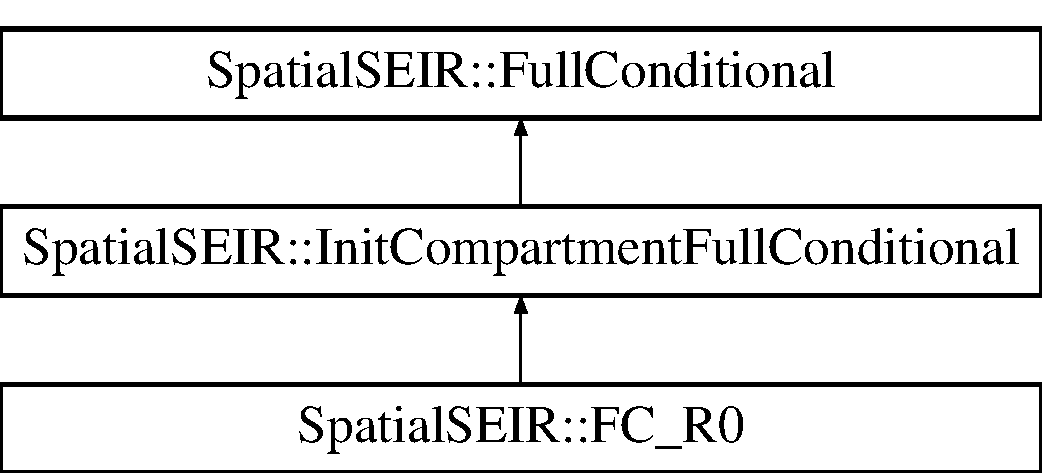
\includegraphics[height=3.000000cm]{classSpatialSEIR_1_1FC__R0}
\end{center}
\end{figure}
\subsection*{Public Member Functions}
\begin{DoxyCompactItemize}
\item 
\hyperlink{classSpatialSEIR_1_1FC__R0_a64aeaca573ebf93865c48e12d10b0a9e}{F\-C\-\_\-\-R0} (\hyperlink{classSpatialSEIR_1_1ModelContext}{Model\-Context} $\ast$\-\_\-context, \hyperlink{classSpatialSEIR_1_1CompartmentalModelMatrix}{Compartmental\-Model\-Matrix} $\ast$\-\_\-\-R, \hyperlink{classSpatialSEIR_1_1CompartmentalModelMatrix}{Compartmental\-Model\-Matrix} $\ast$\-\_\-\-S, \hyperlink{classSpatialSEIR_1_1CompartmentalModelMatrix}{Compartmental\-Model\-Matrix} $\ast$\-\_\-\-S\-\_\-star, \hyperlink{classSpatialSEIR_1_1CompartmentalModelMatrix}{Compartmental\-Model\-Matrix} $\ast$\-\_\-\-E\-\_\-star, \hyperlink{classSpatialSEIR_1_1CompartmentalModelMatrix}{Compartmental\-Model\-Matrix} $\ast$\-\_\-\-R\-\_\-star, \hyperlink{classSpatialSEIR_1_1InitData}{Init\-Data} $\ast$\-\_\-\-A0, double $\ast$\-\_\-p\-\_\-rs, double $\ast$\-\_\-p\-\_\-se, double \hyperlink{classSpatialSEIR_1_1FullConditional_a150ee031af8d086ad0a04b13630a110f}{slice\-Width})
\item 
virtual \hyperlink{classSpatialSEIR_1_1FC__R0_a5d86241914862fb692ffbffb8d1798f3}{$\sim$\-F\-C\-\_\-\-R0} ()
\item 
virtual int \hyperlink{classSpatialSEIR_1_1FC__R0_a0a7321f7437898caad90229e67ce7e12}{eval\-C\-P\-U} ()
\item 
virtual int \hyperlink{classSpatialSEIR_1_1FC__R0_a36373b69de6603391aceb7c326b2cc00}{eval\-O\-C\-L} ()
\item 
virtual void \hyperlink{classSpatialSEIR_1_1FC__R0_afee9585fb8a21f38002912896c85b529}{sample} (int verbose)
\item 
virtual long double \hyperlink{classSpatialSEIR_1_1FC__R0_ab52e48b7be8eb46258602b0d1467ff08}{get\-Value} ()
\item 
virtual void \hyperlink{classSpatialSEIR_1_1FC__R0_a6b21261ddd1928e70dfea6ef25d553bd}{set\-Value} (long double \hyperlink{classSpatialSEIR_1_1FC__R0_a9ef45e653aff78f2fc3e589d1efbfdf2}{value})
\item 
virtual int \hyperlink{classSpatialSEIR_1_1FC__R0_a651e144af6767ba90b59ae04f3164c28}{calculate\-Relevant\-Compartments} ()
\item 
virtual int \hyperlink{classSpatialSEIR_1_1FC__R0_ad94da8ac1a1b746f1902e709d4f81634}{calculate\-Relevant\-Compartments\-\_\-\-O\-C\-L} ()
\end{DoxyCompactItemize}
\subsection*{Public Attributes}
\begin{DoxyCompactItemize}
\item 
\hyperlink{classSpatialSEIR_1_1ModelContext}{Model\-Context} $\ast$$\ast$ \hyperlink{classSpatialSEIR_1_1FC__R0_add24ef73a930cd4f82a2bd742dd4391c}{context}
\item 
\hyperlink{classSpatialSEIR_1_1CompartmentalModelMatrix}{Compartmental\-Model\-Matrix} $\ast$$\ast$ \hyperlink{classSpatialSEIR_1_1FC__R0_a9f63d92307651fc78bae13c5c6801f60}{R}
\item 
\hyperlink{classSpatialSEIR_1_1CompartmentalModelMatrix}{Compartmental\-Model\-Matrix} $\ast$$\ast$ \hyperlink{classSpatialSEIR_1_1FC__R0_a16109df358db796d8f6eefd6a82dbf9f}{S}
\item 
\hyperlink{classSpatialSEIR_1_1CompartmentalModelMatrix}{Compartmental\-Model\-Matrix} $\ast$$\ast$ \hyperlink{classSpatialSEIR_1_1FC__R0_abec5870b4f34a144d70be8e8dbe8119a}{S\-\_\-star}
\item 
\hyperlink{classSpatialSEIR_1_1CompartmentalModelMatrix}{Compartmental\-Model\-Matrix} $\ast$$\ast$ \hyperlink{classSpatialSEIR_1_1FC__R0_a25b1a9ba08198ad0a8b518ed15889294}{E\-\_\-star}
\item 
\hyperlink{classSpatialSEIR_1_1CompartmentalModelMatrix}{Compartmental\-Model\-Matrix} $\ast$$\ast$ \hyperlink{classSpatialSEIR_1_1FC__R0_a8596e0fe8d0489613f9e6c0687b9f9f9}{R\-\_\-star}
\item 
\hyperlink{classSpatialSEIR_1_1InitData}{Init\-Data} $\ast$$\ast$ \hyperlink{classSpatialSEIR_1_1FC__R0_a9a1b73671ac1afcd6c2df5246725498d}{A0}
\item 
double $\ast$$\ast$ \hyperlink{classSpatialSEIR_1_1FC__R0_aa84194ed97d0f2f1c476ca13b5d99ec3}{p\-\_\-rs}
\item 
double $\ast$$\ast$ \hyperlink{classSpatialSEIR_1_1FC__R0_ab38fec9975fe0137fec522b1e78874d0}{p\-\_\-se}
\item 
long double $\ast$ \hyperlink{classSpatialSEIR_1_1FC__R0_a9ef45e653aff78f2fc3e589d1efbfdf2}{value}
\end{DoxyCompactItemize}


\subsection{Detailed Description}
\hyperlink{classSpatialSEIR_1_1FC__R0}{F\-C\-\_\-\-R0} gives the full conditional distribution for the vector of initially removed/recovered individuals. 

\subsection{Constructor \& Destructor Documentation}
\hypertarget{classSpatialSEIR_1_1FC__R0_a64aeaca573ebf93865c48e12d10b0a9e}{\index{Spatial\-S\-E\-I\-R\-::\-F\-C\-\_\-\-R0@{Spatial\-S\-E\-I\-R\-::\-F\-C\-\_\-\-R0}!F\-C\-\_\-\-R0@{F\-C\-\_\-\-R0}}
\index{F\-C\-\_\-\-R0@{F\-C\-\_\-\-R0}!SpatialSEIR::FC_R0@{Spatial\-S\-E\-I\-R\-::\-F\-C\-\_\-\-R0}}
\subsubsection[{F\-C\-\_\-\-R0}]{\setlength{\rightskip}{0pt plus 5cm}Spatial\-S\-E\-I\-R\-::\-F\-C\-\_\-\-R0\-::\-F\-C\-\_\-\-R0 (
\begin{DoxyParamCaption}
\item[{{\bf Model\-Context} $\ast$}]{\-\_\-context, }
\item[{{\bf Compartmental\-Model\-Matrix} $\ast$}]{\-\_\-\-R, }
\item[{{\bf Compartmental\-Model\-Matrix} $\ast$}]{\-\_\-\-S, }
\item[{{\bf Compartmental\-Model\-Matrix} $\ast$}]{\-\_\-\-S\-\_\-star, }
\item[{{\bf Compartmental\-Model\-Matrix} $\ast$}]{\-\_\-\-E\-\_\-star, }
\item[{{\bf Compartmental\-Model\-Matrix} $\ast$}]{\-\_\-\-R\-\_\-star, }
\item[{{\bf Init\-Data} $\ast$}]{\-\_\-\-A0, }
\item[{double $\ast$}]{\-\_\-p\-\_\-rs, }
\item[{double $\ast$}]{\-\_\-p\-\_\-se, }
\item[{double}]{slice\-Width}
\end{DoxyParamCaption}
)}}\label{classSpatialSEIR_1_1FC__R0_a64aeaca573ebf93865c48e12d10b0a9e}
\hypertarget{classSpatialSEIR_1_1FC__R0_a5d86241914862fb692ffbffb8d1798f3}{\index{Spatial\-S\-E\-I\-R\-::\-F\-C\-\_\-\-R0@{Spatial\-S\-E\-I\-R\-::\-F\-C\-\_\-\-R0}!$\sim$\-F\-C\-\_\-\-R0@{$\sim$\-F\-C\-\_\-\-R0}}
\index{$\sim$\-F\-C\-\_\-\-R0@{$\sim$\-F\-C\-\_\-\-R0}!SpatialSEIR::FC_R0@{Spatial\-S\-E\-I\-R\-::\-F\-C\-\_\-\-R0}}
\subsubsection[{$\sim$\-F\-C\-\_\-\-R0}]{\setlength{\rightskip}{0pt plus 5cm}Spatial\-S\-E\-I\-R\-::\-F\-C\-\_\-\-R0\-::$\sim$\-F\-C\-\_\-\-R0 (
\begin{DoxyParamCaption}
{}
\end{DoxyParamCaption}
)\hspace{0.3cm}{\ttfamily [virtual]}}}\label{classSpatialSEIR_1_1FC__R0_a5d86241914862fb692ffbffb8d1798f3}


\subsection{Member Function Documentation}
\hypertarget{classSpatialSEIR_1_1FC__R0_a651e144af6767ba90b59ae04f3164c28}{\index{Spatial\-S\-E\-I\-R\-::\-F\-C\-\_\-\-R0@{Spatial\-S\-E\-I\-R\-::\-F\-C\-\_\-\-R0}!calculate\-Relevant\-Compartments@{calculate\-Relevant\-Compartments}}
\index{calculate\-Relevant\-Compartments@{calculate\-Relevant\-Compartments}!SpatialSEIR::FC_R0@{Spatial\-S\-E\-I\-R\-::\-F\-C\-\_\-\-R0}}
\subsubsection[{calculate\-Relevant\-Compartments}]{\setlength{\rightskip}{0pt plus 5cm}int Spatial\-S\-E\-I\-R\-::\-F\-C\-\_\-\-R0\-::calculate\-Relevant\-Compartments (
\begin{DoxyParamCaption}
{}
\end{DoxyParamCaption}
)\hspace{0.3cm}{\ttfamily [virtual]}}}\label{classSpatialSEIR_1_1FC__R0_a651e144af6767ba90b59ae04f3164c28}


Implements \hyperlink{classSpatialSEIR_1_1InitCompartmentFullConditional_a3fab33c4f5b857998fd928a00cea09e7}{Spatial\-S\-E\-I\-R\-::\-Init\-Compartment\-Full\-Conditional}.

\hypertarget{classSpatialSEIR_1_1FC__R0_ad94da8ac1a1b746f1902e709d4f81634}{\index{Spatial\-S\-E\-I\-R\-::\-F\-C\-\_\-\-R0@{Spatial\-S\-E\-I\-R\-::\-F\-C\-\_\-\-R0}!calculate\-Relevant\-Compartments\-\_\-\-O\-C\-L@{calculate\-Relevant\-Compartments\-\_\-\-O\-C\-L}}
\index{calculate\-Relevant\-Compartments\-\_\-\-O\-C\-L@{calculate\-Relevant\-Compartments\-\_\-\-O\-C\-L}!SpatialSEIR::FC_R0@{Spatial\-S\-E\-I\-R\-::\-F\-C\-\_\-\-R0}}
\subsubsection[{calculate\-Relevant\-Compartments\-\_\-\-O\-C\-L}]{\setlength{\rightskip}{0pt plus 5cm}int Spatial\-S\-E\-I\-R\-::\-F\-C\-\_\-\-R0\-::calculate\-Relevant\-Compartments\-\_\-\-O\-C\-L (
\begin{DoxyParamCaption}
{}
\end{DoxyParamCaption}
)\hspace{0.3cm}{\ttfamily [virtual]}}}\label{classSpatialSEIR_1_1FC__R0_ad94da8ac1a1b746f1902e709d4f81634}


Implements \hyperlink{classSpatialSEIR_1_1InitCompartmentFullConditional_aa4eae1aafbcdc4819be2e520d600dedf}{Spatial\-S\-E\-I\-R\-::\-Init\-Compartment\-Full\-Conditional}.

\hypertarget{classSpatialSEIR_1_1FC__R0_a0a7321f7437898caad90229e67ce7e12}{\index{Spatial\-S\-E\-I\-R\-::\-F\-C\-\_\-\-R0@{Spatial\-S\-E\-I\-R\-::\-F\-C\-\_\-\-R0}!eval\-C\-P\-U@{eval\-C\-P\-U}}
\index{eval\-C\-P\-U@{eval\-C\-P\-U}!SpatialSEIR::FC_R0@{Spatial\-S\-E\-I\-R\-::\-F\-C\-\_\-\-R0}}
\subsubsection[{eval\-C\-P\-U}]{\setlength{\rightskip}{0pt plus 5cm}int Spatial\-S\-E\-I\-R\-::\-F\-C\-\_\-\-R0\-::eval\-C\-P\-U (
\begin{DoxyParamCaption}
{}
\end{DoxyParamCaption}
)\hspace{0.3cm}{\ttfamily [virtual]}}}\label{classSpatialSEIR_1_1FC__R0_a0a7321f7437898caad90229e67ce7e12}


Implements \hyperlink{classSpatialSEIR_1_1InitCompartmentFullConditional_a25fc6e3ac2cb71a6e115ce3235fd8de0}{Spatial\-S\-E\-I\-R\-::\-Init\-Compartment\-Full\-Conditional}.

\hypertarget{classSpatialSEIR_1_1FC__R0_a36373b69de6603391aceb7c326b2cc00}{\index{Spatial\-S\-E\-I\-R\-::\-F\-C\-\_\-\-R0@{Spatial\-S\-E\-I\-R\-::\-F\-C\-\_\-\-R0}!eval\-O\-C\-L@{eval\-O\-C\-L}}
\index{eval\-O\-C\-L@{eval\-O\-C\-L}!SpatialSEIR::FC_R0@{Spatial\-S\-E\-I\-R\-::\-F\-C\-\_\-\-R0}}
\subsubsection[{eval\-O\-C\-L}]{\setlength{\rightskip}{0pt plus 5cm}int Spatial\-S\-E\-I\-R\-::\-F\-C\-\_\-\-R0\-::eval\-O\-C\-L (
\begin{DoxyParamCaption}
{}
\end{DoxyParamCaption}
)\hspace{0.3cm}{\ttfamily [virtual]}}}\label{classSpatialSEIR_1_1FC__R0_a36373b69de6603391aceb7c326b2cc00}


Implements \hyperlink{classSpatialSEIR_1_1InitCompartmentFullConditional_a2f0c4b5628e2f2074c1a84ea6349a754}{Spatial\-S\-E\-I\-R\-::\-Init\-Compartment\-Full\-Conditional}.

\hypertarget{classSpatialSEIR_1_1FC__R0_ab52e48b7be8eb46258602b0d1467ff08}{\index{Spatial\-S\-E\-I\-R\-::\-F\-C\-\_\-\-R0@{Spatial\-S\-E\-I\-R\-::\-F\-C\-\_\-\-R0}!get\-Value@{get\-Value}}
\index{get\-Value@{get\-Value}!SpatialSEIR::FC_R0@{Spatial\-S\-E\-I\-R\-::\-F\-C\-\_\-\-R0}}
\subsubsection[{get\-Value}]{\setlength{\rightskip}{0pt plus 5cm}long double Spatial\-S\-E\-I\-R\-::\-F\-C\-\_\-\-R0\-::get\-Value (
\begin{DoxyParamCaption}
{}
\end{DoxyParamCaption}
)\hspace{0.3cm}{\ttfamily [virtual]}}}\label{classSpatialSEIR_1_1FC__R0_ab52e48b7be8eb46258602b0d1467ff08}


Implements \hyperlink{classSpatialSEIR_1_1InitCompartmentFullConditional_aadb3975a791221136e6c4be5e016d9f1}{Spatial\-S\-E\-I\-R\-::\-Init\-Compartment\-Full\-Conditional}.

\hypertarget{classSpatialSEIR_1_1FC__R0_afee9585fb8a21f38002912896c85b529}{\index{Spatial\-S\-E\-I\-R\-::\-F\-C\-\_\-\-R0@{Spatial\-S\-E\-I\-R\-::\-F\-C\-\_\-\-R0}!sample@{sample}}
\index{sample@{sample}!SpatialSEIR::FC_R0@{Spatial\-S\-E\-I\-R\-::\-F\-C\-\_\-\-R0}}
\subsubsection[{sample}]{\setlength{\rightskip}{0pt plus 5cm}void Spatial\-S\-E\-I\-R\-::\-F\-C\-\_\-\-R0\-::sample (
\begin{DoxyParamCaption}
\item[{int}]{verbose}
\end{DoxyParamCaption}
)\hspace{0.3cm}{\ttfamily [virtual]}}}\label{classSpatialSEIR_1_1FC__R0_afee9585fb8a21f38002912896c85b529}


Implements \hyperlink{classSpatialSEIR_1_1InitCompartmentFullConditional_a03bcc440fa87265336980f3e833f59f2}{Spatial\-S\-E\-I\-R\-::\-Init\-Compartment\-Full\-Conditional}.

\hypertarget{classSpatialSEIR_1_1FC__R0_a6b21261ddd1928e70dfea6ef25d553bd}{\index{Spatial\-S\-E\-I\-R\-::\-F\-C\-\_\-\-R0@{Spatial\-S\-E\-I\-R\-::\-F\-C\-\_\-\-R0}!set\-Value@{set\-Value}}
\index{set\-Value@{set\-Value}!SpatialSEIR::FC_R0@{Spatial\-S\-E\-I\-R\-::\-F\-C\-\_\-\-R0}}
\subsubsection[{set\-Value}]{\setlength{\rightskip}{0pt plus 5cm}void Spatial\-S\-E\-I\-R\-::\-F\-C\-\_\-\-R0\-::set\-Value (
\begin{DoxyParamCaption}
\item[{long double}]{value}
\end{DoxyParamCaption}
)\hspace{0.3cm}{\ttfamily [virtual]}}}\label{classSpatialSEIR_1_1FC__R0_a6b21261ddd1928e70dfea6ef25d553bd}


Implements \hyperlink{classSpatialSEIR_1_1InitCompartmentFullConditional_acbc03a68f5c67beacefadcc3c22c1d88}{Spatial\-S\-E\-I\-R\-::\-Init\-Compartment\-Full\-Conditional}.



\subsection{Member Data Documentation}
\hypertarget{classSpatialSEIR_1_1FC__R0_a9a1b73671ac1afcd6c2df5246725498d}{\index{Spatial\-S\-E\-I\-R\-::\-F\-C\-\_\-\-R0@{Spatial\-S\-E\-I\-R\-::\-F\-C\-\_\-\-R0}!A0@{A0}}
\index{A0@{A0}!SpatialSEIR::FC_R0@{Spatial\-S\-E\-I\-R\-::\-F\-C\-\_\-\-R0}}
\subsubsection[{A0}]{\setlength{\rightskip}{0pt plus 5cm}{\bf Init\-Data}$\ast$$\ast$ Spatial\-S\-E\-I\-R\-::\-F\-C\-\_\-\-R0\-::\-A0}}\label{classSpatialSEIR_1_1FC__R0_a9a1b73671ac1afcd6c2df5246725498d}
\hypertarget{classSpatialSEIR_1_1FC__R0_add24ef73a930cd4f82a2bd742dd4391c}{\index{Spatial\-S\-E\-I\-R\-::\-F\-C\-\_\-\-R0@{Spatial\-S\-E\-I\-R\-::\-F\-C\-\_\-\-R0}!context@{context}}
\index{context@{context}!SpatialSEIR::FC_R0@{Spatial\-S\-E\-I\-R\-::\-F\-C\-\_\-\-R0}}
\subsubsection[{context}]{\setlength{\rightskip}{0pt plus 5cm}{\bf Model\-Context}$\ast$$\ast$ Spatial\-S\-E\-I\-R\-::\-F\-C\-\_\-\-R0\-::context}}\label{classSpatialSEIR_1_1FC__R0_add24ef73a930cd4f82a2bd742dd4391c}
\hypertarget{classSpatialSEIR_1_1FC__R0_a25b1a9ba08198ad0a8b518ed15889294}{\index{Spatial\-S\-E\-I\-R\-::\-F\-C\-\_\-\-R0@{Spatial\-S\-E\-I\-R\-::\-F\-C\-\_\-\-R0}!E\-\_\-star@{E\-\_\-star}}
\index{E\-\_\-star@{E\-\_\-star}!SpatialSEIR::FC_R0@{Spatial\-S\-E\-I\-R\-::\-F\-C\-\_\-\-R0}}
\subsubsection[{E\-\_\-star}]{\setlength{\rightskip}{0pt plus 5cm}{\bf Compartmental\-Model\-Matrix}$\ast$$\ast$ Spatial\-S\-E\-I\-R\-::\-F\-C\-\_\-\-R0\-::\-E\-\_\-star}}\label{classSpatialSEIR_1_1FC__R0_a25b1a9ba08198ad0a8b518ed15889294}
\hypertarget{classSpatialSEIR_1_1FC__R0_aa84194ed97d0f2f1c476ca13b5d99ec3}{\index{Spatial\-S\-E\-I\-R\-::\-F\-C\-\_\-\-R0@{Spatial\-S\-E\-I\-R\-::\-F\-C\-\_\-\-R0}!p\-\_\-rs@{p\-\_\-rs}}
\index{p\-\_\-rs@{p\-\_\-rs}!SpatialSEIR::FC_R0@{Spatial\-S\-E\-I\-R\-::\-F\-C\-\_\-\-R0}}
\subsubsection[{p\-\_\-rs}]{\setlength{\rightskip}{0pt plus 5cm}double$\ast$$\ast$ Spatial\-S\-E\-I\-R\-::\-F\-C\-\_\-\-R0\-::p\-\_\-rs}}\label{classSpatialSEIR_1_1FC__R0_aa84194ed97d0f2f1c476ca13b5d99ec3}
\hypertarget{classSpatialSEIR_1_1FC__R0_ab38fec9975fe0137fec522b1e78874d0}{\index{Spatial\-S\-E\-I\-R\-::\-F\-C\-\_\-\-R0@{Spatial\-S\-E\-I\-R\-::\-F\-C\-\_\-\-R0}!p\-\_\-se@{p\-\_\-se}}
\index{p\-\_\-se@{p\-\_\-se}!SpatialSEIR::FC_R0@{Spatial\-S\-E\-I\-R\-::\-F\-C\-\_\-\-R0}}
\subsubsection[{p\-\_\-se}]{\setlength{\rightskip}{0pt plus 5cm}double$\ast$$\ast$ Spatial\-S\-E\-I\-R\-::\-F\-C\-\_\-\-R0\-::p\-\_\-se}}\label{classSpatialSEIR_1_1FC__R0_ab38fec9975fe0137fec522b1e78874d0}
\hypertarget{classSpatialSEIR_1_1FC__R0_a9f63d92307651fc78bae13c5c6801f60}{\index{Spatial\-S\-E\-I\-R\-::\-F\-C\-\_\-\-R0@{Spatial\-S\-E\-I\-R\-::\-F\-C\-\_\-\-R0}!R@{R}}
\index{R@{R}!SpatialSEIR::FC_R0@{Spatial\-S\-E\-I\-R\-::\-F\-C\-\_\-\-R0}}
\subsubsection[{R}]{\setlength{\rightskip}{0pt plus 5cm}{\bf Compartmental\-Model\-Matrix}$\ast$$\ast$ Spatial\-S\-E\-I\-R\-::\-F\-C\-\_\-\-R0\-::\-R}}\label{classSpatialSEIR_1_1FC__R0_a9f63d92307651fc78bae13c5c6801f60}
\hypertarget{classSpatialSEIR_1_1FC__R0_a8596e0fe8d0489613f9e6c0687b9f9f9}{\index{Spatial\-S\-E\-I\-R\-::\-F\-C\-\_\-\-R0@{Spatial\-S\-E\-I\-R\-::\-F\-C\-\_\-\-R0}!R\-\_\-star@{R\-\_\-star}}
\index{R\-\_\-star@{R\-\_\-star}!SpatialSEIR::FC_R0@{Spatial\-S\-E\-I\-R\-::\-F\-C\-\_\-\-R0}}
\subsubsection[{R\-\_\-star}]{\setlength{\rightskip}{0pt plus 5cm}{\bf Compartmental\-Model\-Matrix}$\ast$$\ast$ Spatial\-S\-E\-I\-R\-::\-F\-C\-\_\-\-R0\-::\-R\-\_\-star}}\label{classSpatialSEIR_1_1FC__R0_a8596e0fe8d0489613f9e6c0687b9f9f9}
\hypertarget{classSpatialSEIR_1_1FC__R0_a16109df358db796d8f6eefd6a82dbf9f}{\index{Spatial\-S\-E\-I\-R\-::\-F\-C\-\_\-\-R0@{Spatial\-S\-E\-I\-R\-::\-F\-C\-\_\-\-R0}!S@{S}}
\index{S@{S}!SpatialSEIR::FC_R0@{Spatial\-S\-E\-I\-R\-::\-F\-C\-\_\-\-R0}}
\subsubsection[{S}]{\setlength{\rightskip}{0pt plus 5cm}{\bf Compartmental\-Model\-Matrix}$\ast$$\ast$ Spatial\-S\-E\-I\-R\-::\-F\-C\-\_\-\-R0\-::\-S}}\label{classSpatialSEIR_1_1FC__R0_a16109df358db796d8f6eefd6a82dbf9f}
\hypertarget{classSpatialSEIR_1_1FC__R0_abec5870b4f34a144d70be8e8dbe8119a}{\index{Spatial\-S\-E\-I\-R\-::\-F\-C\-\_\-\-R0@{Spatial\-S\-E\-I\-R\-::\-F\-C\-\_\-\-R0}!S\-\_\-star@{S\-\_\-star}}
\index{S\-\_\-star@{S\-\_\-star}!SpatialSEIR::FC_R0@{Spatial\-S\-E\-I\-R\-::\-F\-C\-\_\-\-R0}}
\subsubsection[{S\-\_\-star}]{\setlength{\rightskip}{0pt plus 5cm}{\bf Compartmental\-Model\-Matrix}$\ast$$\ast$ Spatial\-S\-E\-I\-R\-::\-F\-C\-\_\-\-R0\-::\-S\-\_\-star}}\label{classSpatialSEIR_1_1FC__R0_abec5870b4f34a144d70be8e8dbe8119a}
\hypertarget{classSpatialSEIR_1_1FC__R0_a9ef45e653aff78f2fc3e589d1efbfdf2}{\index{Spatial\-S\-E\-I\-R\-::\-F\-C\-\_\-\-R0@{Spatial\-S\-E\-I\-R\-::\-F\-C\-\_\-\-R0}!value@{value}}
\index{value@{value}!SpatialSEIR::FC_R0@{Spatial\-S\-E\-I\-R\-::\-F\-C\-\_\-\-R0}}
\subsubsection[{value}]{\setlength{\rightskip}{0pt plus 5cm}long double$\ast$ Spatial\-S\-E\-I\-R\-::\-F\-C\-\_\-\-R0\-::value}}\label{classSpatialSEIR_1_1FC__R0_a9ef45e653aff78f2fc3e589d1efbfdf2}


The documentation for this class was generated from the following files\-:\begin{DoxyCompactItemize}
\item 
lib\-Spatial\-S\-E\-I\-R/include/\-Full\-Conditionals/\hyperlink{LSS__FC__R0_8hpp}{L\-S\-S\-\_\-\-F\-C\-\_\-\-R0.\-hpp}\item 
lib\-Spatial\-S\-E\-I\-R/src/\-Full\-Conditionals/\hyperlink{FC__R0_8cpp}{F\-C\-\_\-\-R0.\-cpp}\end{DoxyCompactItemize}

\hypertarget{classSpatialSEIR_1_1FC__R__Star}{\section{Spatial\-S\-E\-I\-R\-:\-:F\-C\-\_\-\-R\-\_\-\-Star Class Reference}
\label{classSpatialSEIR_1_1FC__R__Star}\index{Spatial\-S\-E\-I\-R\-::\-F\-C\-\_\-\-R\-\_\-\-Star@{Spatial\-S\-E\-I\-R\-::\-F\-C\-\_\-\-R\-\_\-\-Star}}
}


{\ttfamily \#include $<$L\-S\-S\-\_\-\-F\-C\-\_\-\-R\-\_\-star.\-hpp$>$}

Inheritance diagram for Spatial\-S\-E\-I\-R\-:\-:F\-C\-\_\-\-R\-\_\-\-Star\-:\begin{figure}[H]
\begin{center}
\leavevmode
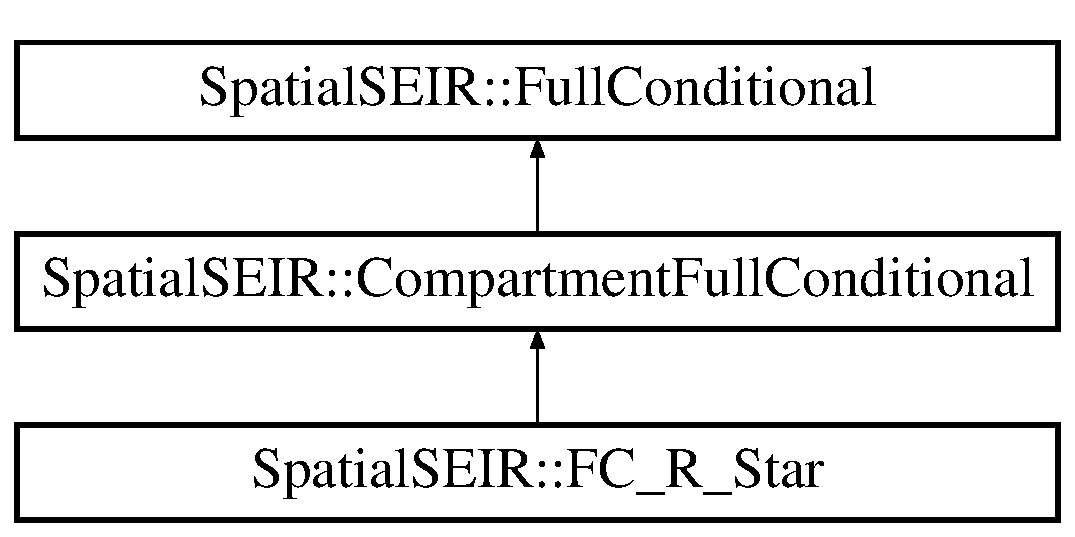
\includegraphics[height=3.000000cm]{classSpatialSEIR_1_1FC__R__Star}
\end{center}
\end{figure}
\subsection*{Public Member Functions}
\begin{DoxyCompactItemize}
\item 
\hyperlink{classSpatialSEIR_1_1FC__R__Star_a487165b3f1aaac332232d06c14104c3d}{F\-C\-\_\-\-R\-\_\-\-Star} (\hyperlink{classSpatialSEIR_1_1ModelContext}{Model\-Context} $\ast$\-\_\-context, \hyperlink{classSpatialSEIR_1_1CompartmentalModelMatrix}{Compartmental\-Model\-Matrix} $\ast$\-\_\-\-R\-\_\-star, \hyperlink{classSpatialSEIR_1_1CompartmentalModelMatrix}{Compartmental\-Model\-Matrix} $\ast$\-\_\-\-R, \hyperlink{classSpatialSEIR_1_1CompartmentalModelMatrix}{Compartmental\-Model\-Matrix} $\ast$\-\_\-\-I, \hyperlink{classSpatialSEIR_1_1CompartmentalModelMatrix}{Compartmental\-Model\-Matrix} $\ast$\-\_\-\-S\-\_\-star, \hyperlink{classSpatialSEIR_1_1CompartmentalModelMatrix}{Compartmental\-Model\-Matrix} $\ast$\-\_\-\-E\-\_\-star, \hyperlink{classSpatialSEIR_1_1CompartmentalModelMatrix}{Compartmental\-Model\-Matrix} $\ast$\-\_\-\-I\-\_\-star, \hyperlink{classSpatialSEIR_1_1CompartmentalModelMatrix}{Compartmental\-Model\-Matrix} $\ast$\-\_\-\-S, \hyperlink{classSpatialSEIR_1_1InitData}{Init\-Data} $\ast$\-\_\-\-A0, double $\ast$\-\_\-p\-\_\-rs, double $\ast$\-\_\-p\-\_\-ir, double $\ast$\-\_\-p\-\_\-se, double \-\_\-steady\-State\-Constraint\-Precision, double \hyperlink{classSpatialSEIR_1_1FullConditional_a150ee031af8d086ad0a04b13630a110f}{slice\-Width})
\item 
\hyperlink{classSpatialSEIR_1_1FC__R__Star_afaac9a9b5d6fded7517b37689cedf8ed}{$\sim$\-F\-C\-\_\-\-R\-\_\-\-Star} ()
\item 
virtual int \hyperlink{classSpatialSEIR_1_1FC__R__Star_a09995dd094fbcc1ee4a02d55e56f8dd6}{eval\-C\-P\-U} ()
\item 
virtual int \hyperlink{classSpatialSEIR_1_1FC__R__Star_aa18118eca9c6fe08ba45449d15a05c64}{eval\-C\-P\-U} (int i, int j)
\item 
virtual int \hyperlink{classSpatialSEIR_1_1FC__R__Star_af019ed60b853ab3ec89b008d0ae566c0}{eval\-O\-C\-L} ()
\item 
virtual void \hyperlink{classSpatialSEIR_1_1FC__R__Star_a18c2097b9333619d95f3e40fbbe070ba}{sample} (int verbose)
\item 
virtual long double \hyperlink{classSpatialSEIR_1_1FC__R__Star_a538786683fedde6a14c85b9081de3c4a}{get\-Value} ()
\item 
virtual void \hyperlink{classSpatialSEIR_1_1FC__R__Star_a751a02d582eae457a5ce86edee57401c}{set\-Value} (long double val)
\item 
virtual int \hyperlink{classSpatialSEIR_1_1FC__R__Star_a530cd0998d1c4c7f2cefe403cedcaf07}{calculate\-Relevant\-Compartments} ()
\item 
virtual int \hyperlink{classSpatialSEIR_1_1FC__R__Star_a3bc76c6c1f22fe238f385ccb3f032e26}{calculate\-Relevant\-Compartments} (int i, int j)
\item 
virtual int \hyperlink{classSpatialSEIR_1_1FC__R__Star_a8e3f3e5cab00e89a2e4fdb21d7460fd4}{calculate\-Relevant\-Compartments\-\_\-\-O\-C\-L} ()
\end{DoxyCompactItemize}
\subsection*{Public Attributes}
\begin{DoxyCompactItemize}
\item 
\hyperlink{classSpatialSEIR_1_1ModelContext}{Model\-Context} $\ast$$\ast$ \hyperlink{classSpatialSEIR_1_1FC__R__Star_ad6f46a048b0ba6b67ccde15d06ed489c}{context}
\item 
\hyperlink{classSpatialSEIR_1_1CompartmentalModelMatrix}{Compartmental\-Model\-Matrix} $\ast$$\ast$ \hyperlink{classSpatialSEIR_1_1FC__R__Star_ae4c0796d43a30d3cd2012cf53efd4b54}{R\-\_\-star}
\item 
\hyperlink{classSpatialSEIR_1_1CompartmentalModelMatrix}{Compartmental\-Model\-Matrix} $\ast$$\ast$ \hyperlink{classSpatialSEIR_1_1FC__R__Star_aaa850a4ce86274b47873855403b89a60}{R}
\item 
\hyperlink{classSpatialSEIR_1_1CompartmentalModelMatrix}{Compartmental\-Model\-Matrix} $\ast$$\ast$ \hyperlink{classSpatialSEIR_1_1FC__R__Star_a469dfad50afd14f2c0d31e0fa2251b07}{I}
\item 
\hyperlink{classSpatialSEIR_1_1CompartmentalModelMatrix}{Compartmental\-Model\-Matrix} $\ast$$\ast$ \hyperlink{classSpatialSEIR_1_1FC__R__Star_ab3302788df387cf8c27a0cb5b6e6af7e}{S\-\_\-star}
\item 
\hyperlink{classSpatialSEIR_1_1CompartmentalModelMatrix}{Compartmental\-Model\-Matrix} $\ast$$\ast$ \hyperlink{classSpatialSEIR_1_1FC__R__Star_a6c0332fc6048b76c493aa6f39ece5b76}{E\-\_\-star}
\item 
\hyperlink{classSpatialSEIR_1_1CompartmentalModelMatrix}{Compartmental\-Model\-Matrix} $\ast$$\ast$ \hyperlink{classSpatialSEIR_1_1FC__R__Star_a09d61de6e39bcfd4ff2e899c19670d55}{I\-\_\-star}
\item 
\hyperlink{classSpatialSEIR_1_1CompartmentalModelMatrix}{Compartmental\-Model\-Matrix} $\ast$$\ast$ \hyperlink{classSpatialSEIR_1_1FC__R__Star_a5a1c636b2e4f98eb690a4cc229bd97dc}{S}
\item 
\hyperlink{classSpatialSEIR_1_1InitData}{Init\-Data} $\ast$$\ast$ \hyperlink{classSpatialSEIR_1_1FC__R__Star_adfe19f14b5c9de7e7ed78ab81351db8e}{A0}
\item 
double $\ast$$\ast$ \hyperlink{classSpatialSEIR_1_1FC__R__Star_a66b5ad04a930d04074ebce5c89cec124}{p\-\_\-rs}
\item 
double $\ast$$\ast$ \hyperlink{classSpatialSEIR_1_1FC__R__Star_ae940ad3ed88ec011e9fecd7de3fc8864}{p\-\_\-ir}
\item 
double $\ast$$\ast$ \hyperlink{classSpatialSEIR_1_1FC__R__Star_a86cece0c58f44462b0f553bf7c8b8af6}{p\-\_\-se}
\item 
long double $\ast$ \hyperlink{classSpatialSEIR_1_1FC__R__Star_ab7dbeeefaeeafdf681e13f19e50055c3}{value}
\item 
double $\ast$ \hyperlink{classSpatialSEIR_1_1FC__R__Star_a495244734c4c39dc118ceef404062c70}{steady\-State\-Constraint\-Precision}
\end{DoxyCompactItemize}


\subsection{Detailed Description}
\hyperlink{classSpatialSEIR_1_1FC__R__Star}{F\-C\-\_\-\-R\-\_\-\-Star} gives the full conditional distribution of R\-\_\-star, the transition matrix capturing individuals moving from the infectious category to the recovered/removed category. 

\subsection{Constructor \& Destructor Documentation}
\hypertarget{classSpatialSEIR_1_1FC__R__Star_a487165b3f1aaac332232d06c14104c3d}{\index{Spatial\-S\-E\-I\-R\-::\-F\-C\-\_\-\-R\-\_\-\-Star@{Spatial\-S\-E\-I\-R\-::\-F\-C\-\_\-\-R\-\_\-\-Star}!F\-C\-\_\-\-R\-\_\-\-Star@{F\-C\-\_\-\-R\-\_\-\-Star}}
\index{F\-C\-\_\-\-R\-\_\-\-Star@{F\-C\-\_\-\-R\-\_\-\-Star}!SpatialSEIR::FC_R_Star@{Spatial\-S\-E\-I\-R\-::\-F\-C\-\_\-\-R\-\_\-\-Star}}
\subsubsection[{F\-C\-\_\-\-R\-\_\-\-Star}]{\setlength{\rightskip}{0pt plus 5cm}Spatial\-S\-E\-I\-R\-::\-F\-C\-\_\-\-R\-\_\-\-Star\-::\-F\-C\-\_\-\-R\-\_\-\-Star (
\begin{DoxyParamCaption}
\item[{{\bf Model\-Context} $\ast$}]{\-\_\-context, }
\item[{{\bf Compartmental\-Model\-Matrix} $\ast$}]{\-\_\-\-R\-\_\-star, }
\item[{{\bf Compartmental\-Model\-Matrix} $\ast$}]{\-\_\-\-R, }
\item[{{\bf Compartmental\-Model\-Matrix} $\ast$}]{\-\_\-\-I, }
\item[{{\bf Compartmental\-Model\-Matrix} $\ast$}]{\-\_\-\-S\-\_\-star, }
\item[{{\bf Compartmental\-Model\-Matrix} $\ast$}]{\-\_\-\-E\-\_\-star, }
\item[{{\bf Compartmental\-Model\-Matrix} $\ast$}]{\-\_\-\-I\-\_\-star, }
\item[{{\bf Compartmental\-Model\-Matrix} $\ast$}]{\-\_\-\-S, }
\item[{{\bf Init\-Data} $\ast$}]{\-\_\-\-A0, }
\item[{double $\ast$}]{\-\_\-p\-\_\-rs, }
\item[{double $\ast$}]{\-\_\-p\-\_\-ir, }
\item[{double $\ast$}]{\-\_\-p\-\_\-se, }
\item[{double}]{\-\_\-steady\-State\-Constraint\-Precision, }
\item[{double}]{slice\-Width}
\end{DoxyParamCaption}
)}}\label{classSpatialSEIR_1_1FC__R__Star_a487165b3f1aaac332232d06c14104c3d}
\hypertarget{classSpatialSEIR_1_1FC__R__Star_afaac9a9b5d6fded7517b37689cedf8ed}{\index{Spatial\-S\-E\-I\-R\-::\-F\-C\-\_\-\-R\-\_\-\-Star@{Spatial\-S\-E\-I\-R\-::\-F\-C\-\_\-\-R\-\_\-\-Star}!$\sim$\-F\-C\-\_\-\-R\-\_\-\-Star@{$\sim$\-F\-C\-\_\-\-R\-\_\-\-Star}}
\index{$\sim$\-F\-C\-\_\-\-R\-\_\-\-Star@{$\sim$\-F\-C\-\_\-\-R\-\_\-\-Star}!SpatialSEIR::FC_R_Star@{Spatial\-S\-E\-I\-R\-::\-F\-C\-\_\-\-R\-\_\-\-Star}}
\subsubsection[{$\sim$\-F\-C\-\_\-\-R\-\_\-\-Star}]{\setlength{\rightskip}{0pt plus 5cm}Spatial\-S\-E\-I\-R\-::\-F\-C\-\_\-\-R\-\_\-\-Star\-::$\sim$\-F\-C\-\_\-\-R\-\_\-\-Star (
\begin{DoxyParamCaption}
{}
\end{DoxyParamCaption}
)}}\label{classSpatialSEIR_1_1FC__R__Star_afaac9a9b5d6fded7517b37689cedf8ed}


\subsection{Member Function Documentation}
\hypertarget{classSpatialSEIR_1_1FC__R__Star_a530cd0998d1c4c7f2cefe403cedcaf07}{\index{Spatial\-S\-E\-I\-R\-::\-F\-C\-\_\-\-R\-\_\-\-Star@{Spatial\-S\-E\-I\-R\-::\-F\-C\-\_\-\-R\-\_\-\-Star}!calculate\-Relevant\-Compartments@{calculate\-Relevant\-Compartments}}
\index{calculate\-Relevant\-Compartments@{calculate\-Relevant\-Compartments}!SpatialSEIR::FC_R_Star@{Spatial\-S\-E\-I\-R\-::\-F\-C\-\_\-\-R\-\_\-\-Star}}
\subsubsection[{calculate\-Relevant\-Compartments}]{\setlength{\rightskip}{0pt plus 5cm}int Spatial\-S\-E\-I\-R\-::\-F\-C\-\_\-\-R\-\_\-\-Star\-::calculate\-Relevant\-Compartments (
\begin{DoxyParamCaption}
{}
\end{DoxyParamCaption}
)\hspace{0.3cm}{\ttfamily [virtual]}}}\label{classSpatialSEIR_1_1FC__R__Star_a530cd0998d1c4c7f2cefe403cedcaf07}


Implements \hyperlink{classSpatialSEIR_1_1CompartmentFullConditional_a71836271b0997117f3b8437c2f55a986}{Spatial\-S\-E\-I\-R\-::\-Compartment\-Full\-Conditional}.

\hypertarget{classSpatialSEIR_1_1FC__R__Star_a3bc76c6c1f22fe238f385ccb3f032e26}{\index{Spatial\-S\-E\-I\-R\-::\-F\-C\-\_\-\-R\-\_\-\-Star@{Spatial\-S\-E\-I\-R\-::\-F\-C\-\_\-\-R\-\_\-\-Star}!calculate\-Relevant\-Compartments@{calculate\-Relevant\-Compartments}}
\index{calculate\-Relevant\-Compartments@{calculate\-Relevant\-Compartments}!SpatialSEIR::FC_R_Star@{Spatial\-S\-E\-I\-R\-::\-F\-C\-\_\-\-R\-\_\-\-Star}}
\subsubsection[{calculate\-Relevant\-Compartments}]{\setlength{\rightskip}{0pt plus 5cm}int Spatial\-S\-E\-I\-R\-::\-F\-C\-\_\-\-R\-\_\-\-Star\-::calculate\-Relevant\-Compartments (
\begin{DoxyParamCaption}
\item[{int}]{i, }
\item[{int}]{j}
\end{DoxyParamCaption}
)\hspace{0.3cm}{\ttfamily [virtual]}}}\label{classSpatialSEIR_1_1FC__R__Star_a3bc76c6c1f22fe238f385ccb3f032e26}


Implements \hyperlink{classSpatialSEIR_1_1CompartmentFullConditional_a21440bf07bd554a2893a328713bfe09f}{Spatial\-S\-E\-I\-R\-::\-Compartment\-Full\-Conditional}.

\hypertarget{classSpatialSEIR_1_1FC__R__Star_a8e3f3e5cab00e89a2e4fdb21d7460fd4}{\index{Spatial\-S\-E\-I\-R\-::\-F\-C\-\_\-\-R\-\_\-\-Star@{Spatial\-S\-E\-I\-R\-::\-F\-C\-\_\-\-R\-\_\-\-Star}!calculate\-Relevant\-Compartments\-\_\-\-O\-C\-L@{calculate\-Relevant\-Compartments\-\_\-\-O\-C\-L}}
\index{calculate\-Relevant\-Compartments\-\_\-\-O\-C\-L@{calculate\-Relevant\-Compartments\-\_\-\-O\-C\-L}!SpatialSEIR::FC_R_Star@{Spatial\-S\-E\-I\-R\-::\-F\-C\-\_\-\-R\-\_\-\-Star}}
\subsubsection[{calculate\-Relevant\-Compartments\-\_\-\-O\-C\-L}]{\setlength{\rightskip}{0pt plus 5cm}int Spatial\-S\-E\-I\-R\-::\-F\-C\-\_\-\-R\-\_\-\-Star\-::calculate\-Relevant\-Compartments\-\_\-\-O\-C\-L (
\begin{DoxyParamCaption}
{}
\end{DoxyParamCaption}
)\hspace{0.3cm}{\ttfamily [virtual]}}}\label{classSpatialSEIR_1_1FC__R__Star_a8e3f3e5cab00e89a2e4fdb21d7460fd4}


Implements \hyperlink{classSpatialSEIR_1_1CompartmentFullConditional_ab873ecc59f7639637113d885ab89bed4}{Spatial\-S\-E\-I\-R\-::\-Compartment\-Full\-Conditional}.

\hypertarget{classSpatialSEIR_1_1FC__R__Star_a09995dd094fbcc1ee4a02d55e56f8dd6}{\index{Spatial\-S\-E\-I\-R\-::\-F\-C\-\_\-\-R\-\_\-\-Star@{Spatial\-S\-E\-I\-R\-::\-F\-C\-\_\-\-R\-\_\-\-Star}!eval\-C\-P\-U@{eval\-C\-P\-U}}
\index{eval\-C\-P\-U@{eval\-C\-P\-U}!SpatialSEIR::FC_R_Star@{Spatial\-S\-E\-I\-R\-::\-F\-C\-\_\-\-R\-\_\-\-Star}}
\subsubsection[{eval\-C\-P\-U}]{\setlength{\rightskip}{0pt plus 5cm}int Spatial\-S\-E\-I\-R\-::\-F\-C\-\_\-\-R\-\_\-\-Star\-::eval\-C\-P\-U (
\begin{DoxyParamCaption}
{}
\end{DoxyParamCaption}
)\hspace{0.3cm}{\ttfamily [virtual]}}}\label{classSpatialSEIR_1_1FC__R__Star_a09995dd094fbcc1ee4a02d55e56f8dd6}


Implements \hyperlink{classSpatialSEIR_1_1CompartmentFullConditional_ad2402c8d7fc0b362482bcd5ceaa035af}{Spatial\-S\-E\-I\-R\-::\-Compartment\-Full\-Conditional}.

\hypertarget{classSpatialSEIR_1_1FC__R__Star_aa18118eca9c6fe08ba45449d15a05c64}{\index{Spatial\-S\-E\-I\-R\-::\-F\-C\-\_\-\-R\-\_\-\-Star@{Spatial\-S\-E\-I\-R\-::\-F\-C\-\_\-\-R\-\_\-\-Star}!eval\-C\-P\-U@{eval\-C\-P\-U}}
\index{eval\-C\-P\-U@{eval\-C\-P\-U}!SpatialSEIR::FC_R_Star@{Spatial\-S\-E\-I\-R\-::\-F\-C\-\_\-\-R\-\_\-\-Star}}
\subsubsection[{eval\-C\-P\-U}]{\setlength{\rightskip}{0pt plus 5cm}int Spatial\-S\-E\-I\-R\-::\-F\-C\-\_\-\-R\-\_\-\-Star\-::eval\-C\-P\-U (
\begin{DoxyParamCaption}
\item[{int}]{i, }
\item[{int}]{j}
\end{DoxyParamCaption}
)\hspace{0.3cm}{\ttfamily [virtual]}}}\label{classSpatialSEIR_1_1FC__R__Star_aa18118eca9c6fe08ba45449d15a05c64}


Implements \hyperlink{classSpatialSEIR_1_1CompartmentFullConditional_a92d48bc8cd13ff048791edbdcc453479}{Spatial\-S\-E\-I\-R\-::\-Compartment\-Full\-Conditional}.

\hypertarget{classSpatialSEIR_1_1FC__R__Star_af019ed60b853ab3ec89b008d0ae566c0}{\index{Spatial\-S\-E\-I\-R\-::\-F\-C\-\_\-\-R\-\_\-\-Star@{Spatial\-S\-E\-I\-R\-::\-F\-C\-\_\-\-R\-\_\-\-Star}!eval\-O\-C\-L@{eval\-O\-C\-L}}
\index{eval\-O\-C\-L@{eval\-O\-C\-L}!SpatialSEIR::FC_R_Star@{Spatial\-S\-E\-I\-R\-::\-F\-C\-\_\-\-R\-\_\-\-Star}}
\subsubsection[{eval\-O\-C\-L}]{\setlength{\rightskip}{0pt plus 5cm}int Spatial\-S\-E\-I\-R\-::\-F\-C\-\_\-\-R\-\_\-\-Star\-::eval\-O\-C\-L (
\begin{DoxyParamCaption}
{}
\end{DoxyParamCaption}
)\hspace{0.3cm}{\ttfamily [virtual]}}}\label{classSpatialSEIR_1_1FC__R__Star_af019ed60b853ab3ec89b008d0ae566c0}


Implements \hyperlink{classSpatialSEIR_1_1CompartmentFullConditional_ac7c7b1191508d49a56ec739449bf93d4}{Spatial\-S\-E\-I\-R\-::\-Compartment\-Full\-Conditional}.

\hypertarget{classSpatialSEIR_1_1FC__R__Star_a538786683fedde6a14c85b9081de3c4a}{\index{Spatial\-S\-E\-I\-R\-::\-F\-C\-\_\-\-R\-\_\-\-Star@{Spatial\-S\-E\-I\-R\-::\-F\-C\-\_\-\-R\-\_\-\-Star}!get\-Value@{get\-Value}}
\index{get\-Value@{get\-Value}!SpatialSEIR::FC_R_Star@{Spatial\-S\-E\-I\-R\-::\-F\-C\-\_\-\-R\-\_\-\-Star}}
\subsubsection[{get\-Value}]{\setlength{\rightskip}{0pt plus 5cm}long double Spatial\-S\-E\-I\-R\-::\-F\-C\-\_\-\-R\-\_\-\-Star\-::get\-Value (
\begin{DoxyParamCaption}
{}
\end{DoxyParamCaption}
)\hspace{0.3cm}{\ttfamily [virtual]}}}\label{classSpatialSEIR_1_1FC__R__Star_a538786683fedde6a14c85b9081de3c4a}


Implements \hyperlink{classSpatialSEIR_1_1CompartmentFullConditional_a28794be23ee7f6fcba96ff2bee63e065}{Spatial\-S\-E\-I\-R\-::\-Compartment\-Full\-Conditional}.

\hypertarget{classSpatialSEIR_1_1FC__R__Star_a18c2097b9333619d95f3e40fbbe070ba}{\index{Spatial\-S\-E\-I\-R\-::\-F\-C\-\_\-\-R\-\_\-\-Star@{Spatial\-S\-E\-I\-R\-::\-F\-C\-\_\-\-R\-\_\-\-Star}!sample@{sample}}
\index{sample@{sample}!SpatialSEIR::FC_R_Star@{Spatial\-S\-E\-I\-R\-::\-F\-C\-\_\-\-R\-\_\-\-Star}}
\subsubsection[{sample}]{\setlength{\rightskip}{0pt plus 5cm}void Spatial\-S\-E\-I\-R\-::\-F\-C\-\_\-\-R\-\_\-\-Star\-::sample (
\begin{DoxyParamCaption}
\item[{int}]{verbose}
\end{DoxyParamCaption}
)\hspace{0.3cm}{\ttfamily [virtual]}}}\label{classSpatialSEIR_1_1FC__R__Star_a18c2097b9333619d95f3e40fbbe070ba}


Implements \hyperlink{classSpatialSEIR_1_1CompartmentFullConditional_a436ae9e47f7a4269f0a78ce225e6b7f3}{Spatial\-S\-E\-I\-R\-::\-Compartment\-Full\-Conditional}.

\hypertarget{classSpatialSEIR_1_1FC__R__Star_a751a02d582eae457a5ce86edee57401c}{\index{Spatial\-S\-E\-I\-R\-::\-F\-C\-\_\-\-R\-\_\-\-Star@{Spatial\-S\-E\-I\-R\-::\-F\-C\-\_\-\-R\-\_\-\-Star}!set\-Value@{set\-Value}}
\index{set\-Value@{set\-Value}!SpatialSEIR::FC_R_Star@{Spatial\-S\-E\-I\-R\-::\-F\-C\-\_\-\-R\-\_\-\-Star}}
\subsubsection[{set\-Value}]{\setlength{\rightskip}{0pt plus 5cm}void Spatial\-S\-E\-I\-R\-::\-F\-C\-\_\-\-R\-\_\-\-Star\-::set\-Value (
\begin{DoxyParamCaption}
\item[{long double}]{val}
\end{DoxyParamCaption}
)\hspace{0.3cm}{\ttfamily [virtual]}}}\label{classSpatialSEIR_1_1FC__R__Star_a751a02d582eae457a5ce86edee57401c}


Implements \hyperlink{classSpatialSEIR_1_1CompartmentFullConditional_a22ab4dcc354c8ebc4f619685bc32dfae}{Spatial\-S\-E\-I\-R\-::\-Compartment\-Full\-Conditional}.



\subsection{Member Data Documentation}
\hypertarget{classSpatialSEIR_1_1FC__R__Star_adfe19f14b5c9de7e7ed78ab81351db8e}{\index{Spatial\-S\-E\-I\-R\-::\-F\-C\-\_\-\-R\-\_\-\-Star@{Spatial\-S\-E\-I\-R\-::\-F\-C\-\_\-\-R\-\_\-\-Star}!A0@{A0}}
\index{A0@{A0}!SpatialSEIR::FC_R_Star@{Spatial\-S\-E\-I\-R\-::\-F\-C\-\_\-\-R\-\_\-\-Star}}
\subsubsection[{A0}]{\setlength{\rightskip}{0pt plus 5cm}{\bf Init\-Data}$\ast$$\ast$ Spatial\-S\-E\-I\-R\-::\-F\-C\-\_\-\-R\-\_\-\-Star\-::\-A0}}\label{classSpatialSEIR_1_1FC__R__Star_adfe19f14b5c9de7e7ed78ab81351db8e}
\hypertarget{classSpatialSEIR_1_1FC__R__Star_ad6f46a048b0ba6b67ccde15d06ed489c}{\index{Spatial\-S\-E\-I\-R\-::\-F\-C\-\_\-\-R\-\_\-\-Star@{Spatial\-S\-E\-I\-R\-::\-F\-C\-\_\-\-R\-\_\-\-Star}!context@{context}}
\index{context@{context}!SpatialSEIR::FC_R_Star@{Spatial\-S\-E\-I\-R\-::\-F\-C\-\_\-\-R\-\_\-\-Star}}
\subsubsection[{context}]{\setlength{\rightskip}{0pt plus 5cm}{\bf Model\-Context}$\ast$$\ast$ Spatial\-S\-E\-I\-R\-::\-F\-C\-\_\-\-R\-\_\-\-Star\-::context}}\label{classSpatialSEIR_1_1FC__R__Star_ad6f46a048b0ba6b67ccde15d06ed489c}
\hypertarget{classSpatialSEIR_1_1FC__R__Star_a6c0332fc6048b76c493aa6f39ece5b76}{\index{Spatial\-S\-E\-I\-R\-::\-F\-C\-\_\-\-R\-\_\-\-Star@{Spatial\-S\-E\-I\-R\-::\-F\-C\-\_\-\-R\-\_\-\-Star}!E\-\_\-star@{E\-\_\-star}}
\index{E\-\_\-star@{E\-\_\-star}!SpatialSEIR::FC_R_Star@{Spatial\-S\-E\-I\-R\-::\-F\-C\-\_\-\-R\-\_\-\-Star}}
\subsubsection[{E\-\_\-star}]{\setlength{\rightskip}{0pt plus 5cm}{\bf Compartmental\-Model\-Matrix}$\ast$$\ast$ Spatial\-S\-E\-I\-R\-::\-F\-C\-\_\-\-R\-\_\-\-Star\-::\-E\-\_\-star}}\label{classSpatialSEIR_1_1FC__R__Star_a6c0332fc6048b76c493aa6f39ece5b76}
\hypertarget{classSpatialSEIR_1_1FC__R__Star_a469dfad50afd14f2c0d31e0fa2251b07}{\index{Spatial\-S\-E\-I\-R\-::\-F\-C\-\_\-\-R\-\_\-\-Star@{Spatial\-S\-E\-I\-R\-::\-F\-C\-\_\-\-R\-\_\-\-Star}!I@{I}}
\index{I@{I}!SpatialSEIR::FC_R_Star@{Spatial\-S\-E\-I\-R\-::\-F\-C\-\_\-\-R\-\_\-\-Star}}
\subsubsection[{I}]{\setlength{\rightskip}{0pt plus 5cm}{\bf Compartmental\-Model\-Matrix}$\ast$$\ast$ Spatial\-S\-E\-I\-R\-::\-F\-C\-\_\-\-R\-\_\-\-Star\-::\-I}}\label{classSpatialSEIR_1_1FC__R__Star_a469dfad50afd14f2c0d31e0fa2251b07}
\hypertarget{classSpatialSEIR_1_1FC__R__Star_a09d61de6e39bcfd4ff2e899c19670d55}{\index{Spatial\-S\-E\-I\-R\-::\-F\-C\-\_\-\-R\-\_\-\-Star@{Spatial\-S\-E\-I\-R\-::\-F\-C\-\_\-\-R\-\_\-\-Star}!I\-\_\-star@{I\-\_\-star}}
\index{I\-\_\-star@{I\-\_\-star}!SpatialSEIR::FC_R_Star@{Spatial\-S\-E\-I\-R\-::\-F\-C\-\_\-\-R\-\_\-\-Star}}
\subsubsection[{I\-\_\-star}]{\setlength{\rightskip}{0pt plus 5cm}{\bf Compartmental\-Model\-Matrix}$\ast$$\ast$ Spatial\-S\-E\-I\-R\-::\-F\-C\-\_\-\-R\-\_\-\-Star\-::\-I\-\_\-star}}\label{classSpatialSEIR_1_1FC__R__Star_a09d61de6e39bcfd4ff2e899c19670d55}
\hypertarget{classSpatialSEIR_1_1FC__R__Star_ae940ad3ed88ec011e9fecd7de3fc8864}{\index{Spatial\-S\-E\-I\-R\-::\-F\-C\-\_\-\-R\-\_\-\-Star@{Spatial\-S\-E\-I\-R\-::\-F\-C\-\_\-\-R\-\_\-\-Star}!p\-\_\-ir@{p\-\_\-ir}}
\index{p\-\_\-ir@{p\-\_\-ir}!SpatialSEIR::FC_R_Star@{Spatial\-S\-E\-I\-R\-::\-F\-C\-\_\-\-R\-\_\-\-Star}}
\subsubsection[{p\-\_\-ir}]{\setlength{\rightskip}{0pt plus 5cm}double$\ast$$\ast$ Spatial\-S\-E\-I\-R\-::\-F\-C\-\_\-\-R\-\_\-\-Star\-::p\-\_\-ir}}\label{classSpatialSEIR_1_1FC__R__Star_ae940ad3ed88ec011e9fecd7de3fc8864}
\hypertarget{classSpatialSEIR_1_1FC__R__Star_a66b5ad04a930d04074ebce5c89cec124}{\index{Spatial\-S\-E\-I\-R\-::\-F\-C\-\_\-\-R\-\_\-\-Star@{Spatial\-S\-E\-I\-R\-::\-F\-C\-\_\-\-R\-\_\-\-Star}!p\-\_\-rs@{p\-\_\-rs}}
\index{p\-\_\-rs@{p\-\_\-rs}!SpatialSEIR::FC_R_Star@{Spatial\-S\-E\-I\-R\-::\-F\-C\-\_\-\-R\-\_\-\-Star}}
\subsubsection[{p\-\_\-rs}]{\setlength{\rightskip}{0pt plus 5cm}double$\ast$$\ast$ Spatial\-S\-E\-I\-R\-::\-F\-C\-\_\-\-R\-\_\-\-Star\-::p\-\_\-rs}}\label{classSpatialSEIR_1_1FC__R__Star_a66b5ad04a930d04074ebce5c89cec124}
\hypertarget{classSpatialSEIR_1_1FC__R__Star_a86cece0c58f44462b0f553bf7c8b8af6}{\index{Spatial\-S\-E\-I\-R\-::\-F\-C\-\_\-\-R\-\_\-\-Star@{Spatial\-S\-E\-I\-R\-::\-F\-C\-\_\-\-R\-\_\-\-Star}!p\-\_\-se@{p\-\_\-se}}
\index{p\-\_\-se@{p\-\_\-se}!SpatialSEIR::FC_R_Star@{Spatial\-S\-E\-I\-R\-::\-F\-C\-\_\-\-R\-\_\-\-Star}}
\subsubsection[{p\-\_\-se}]{\setlength{\rightskip}{0pt plus 5cm}double$\ast$$\ast$ Spatial\-S\-E\-I\-R\-::\-F\-C\-\_\-\-R\-\_\-\-Star\-::p\-\_\-se}}\label{classSpatialSEIR_1_1FC__R__Star_a86cece0c58f44462b0f553bf7c8b8af6}
\hypertarget{classSpatialSEIR_1_1FC__R__Star_aaa850a4ce86274b47873855403b89a60}{\index{Spatial\-S\-E\-I\-R\-::\-F\-C\-\_\-\-R\-\_\-\-Star@{Spatial\-S\-E\-I\-R\-::\-F\-C\-\_\-\-R\-\_\-\-Star}!R@{R}}
\index{R@{R}!SpatialSEIR::FC_R_Star@{Spatial\-S\-E\-I\-R\-::\-F\-C\-\_\-\-R\-\_\-\-Star}}
\subsubsection[{R}]{\setlength{\rightskip}{0pt plus 5cm}{\bf Compartmental\-Model\-Matrix}$\ast$$\ast$ Spatial\-S\-E\-I\-R\-::\-F\-C\-\_\-\-R\-\_\-\-Star\-::\-R}}\label{classSpatialSEIR_1_1FC__R__Star_aaa850a4ce86274b47873855403b89a60}
\hypertarget{classSpatialSEIR_1_1FC__R__Star_ae4c0796d43a30d3cd2012cf53efd4b54}{\index{Spatial\-S\-E\-I\-R\-::\-F\-C\-\_\-\-R\-\_\-\-Star@{Spatial\-S\-E\-I\-R\-::\-F\-C\-\_\-\-R\-\_\-\-Star}!R\-\_\-star@{R\-\_\-star}}
\index{R\-\_\-star@{R\-\_\-star}!SpatialSEIR::FC_R_Star@{Spatial\-S\-E\-I\-R\-::\-F\-C\-\_\-\-R\-\_\-\-Star}}
\subsubsection[{R\-\_\-star}]{\setlength{\rightskip}{0pt plus 5cm}{\bf Compartmental\-Model\-Matrix}$\ast$$\ast$ Spatial\-S\-E\-I\-R\-::\-F\-C\-\_\-\-R\-\_\-\-Star\-::\-R\-\_\-star}}\label{classSpatialSEIR_1_1FC__R__Star_ae4c0796d43a30d3cd2012cf53efd4b54}
\hypertarget{classSpatialSEIR_1_1FC__R__Star_a5a1c636b2e4f98eb690a4cc229bd97dc}{\index{Spatial\-S\-E\-I\-R\-::\-F\-C\-\_\-\-R\-\_\-\-Star@{Spatial\-S\-E\-I\-R\-::\-F\-C\-\_\-\-R\-\_\-\-Star}!S@{S}}
\index{S@{S}!SpatialSEIR::FC_R_Star@{Spatial\-S\-E\-I\-R\-::\-F\-C\-\_\-\-R\-\_\-\-Star}}
\subsubsection[{S}]{\setlength{\rightskip}{0pt plus 5cm}{\bf Compartmental\-Model\-Matrix}$\ast$$\ast$ Spatial\-S\-E\-I\-R\-::\-F\-C\-\_\-\-R\-\_\-\-Star\-::\-S}}\label{classSpatialSEIR_1_1FC__R__Star_a5a1c636b2e4f98eb690a4cc229bd97dc}
\hypertarget{classSpatialSEIR_1_1FC__R__Star_ab3302788df387cf8c27a0cb5b6e6af7e}{\index{Spatial\-S\-E\-I\-R\-::\-F\-C\-\_\-\-R\-\_\-\-Star@{Spatial\-S\-E\-I\-R\-::\-F\-C\-\_\-\-R\-\_\-\-Star}!S\-\_\-star@{S\-\_\-star}}
\index{S\-\_\-star@{S\-\_\-star}!SpatialSEIR::FC_R_Star@{Spatial\-S\-E\-I\-R\-::\-F\-C\-\_\-\-R\-\_\-\-Star}}
\subsubsection[{S\-\_\-star}]{\setlength{\rightskip}{0pt plus 5cm}{\bf Compartmental\-Model\-Matrix}$\ast$$\ast$ Spatial\-S\-E\-I\-R\-::\-F\-C\-\_\-\-R\-\_\-\-Star\-::\-S\-\_\-star}}\label{classSpatialSEIR_1_1FC__R__Star_ab3302788df387cf8c27a0cb5b6e6af7e}
\hypertarget{classSpatialSEIR_1_1FC__R__Star_a495244734c4c39dc118ceef404062c70}{\index{Spatial\-S\-E\-I\-R\-::\-F\-C\-\_\-\-R\-\_\-\-Star@{Spatial\-S\-E\-I\-R\-::\-F\-C\-\_\-\-R\-\_\-\-Star}!steady\-State\-Constraint\-Precision@{steady\-State\-Constraint\-Precision}}
\index{steady\-State\-Constraint\-Precision@{steady\-State\-Constraint\-Precision}!SpatialSEIR::FC_R_Star@{Spatial\-S\-E\-I\-R\-::\-F\-C\-\_\-\-R\-\_\-\-Star}}
\subsubsection[{steady\-State\-Constraint\-Precision}]{\setlength{\rightskip}{0pt plus 5cm}double$\ast$ Spatial\-S\-E\-I\-R\-::\-F\-C\-\_\-\-R\-\_\-\-Star\-::steady\-State\-Constraint\-Precision}}\label{classSpatialSEIR_1_1FC__R__Star_a495244734c4c39dc118ceef404062c70}
\hypertarget{classSpatialSEIR_1_1FC__R__Star_ab7dbeeefaeeafdf681e13f19e50055c3}{\index{Spatial\-S\-E\-I\-R\-::\-F\-C\-\_\-\-R\-\_\-\-Star@{Spatial\-S\-E\-I\-R\-::\-F\-C\-\_\-\-R\-\_\-\-Star}!value@{value}}
\index{value@{value}!SpatialSEIR::FC_R_Star@{Spatial\-S\-E\-I\-R\-::\-F\-C\-\_\-\-R\-\_\-\-Star}}
\subsubsection[{value}]{\setlength{\rightskip}{0pt plus 5cm}long double$\ast$ Spatial\-S\-E\-I\-R\-::\-F\-C\-\_\-\-R\-\_\-\-Star\-::value}}\label{classSpatialSEIR_1_1FC__R__Star_ab7dbeeefaeeafdf681e13f19e50055c3}


The documentation for this class was generated from the following files\-:\begin{DoxyCompactItemize}
\item 
lib\-Spatial\-S\-E\-I\-R/include/\-Full\-Conditionals/\hyperlink{LSS__FC__R__star_8hpp}{L\-S\-S\-\_\-\-F\-C\-\_\-\-R\-\_\-star.\-hpp}\item 
lib\-Spatial\-S\-E\-I\-R/src/\-Full\-Conditionals/\hyperlink{FC__R__star_8cpp}{F\-C\-\_\-\-R\-\_\-star.\-cpp}\end{DoxyCompactItemize}

\hypertarget{classSpatialSEIR_1_1FC__Rho}{\section{Spatial\-S\-E\-I\-R\-:\-:F\-C\-\_\-\-Rho Class Reference}
\label{classSpatialSEIR_1_1FC__Rho}\index{Spatial\-S\-E\-I\-R\-::\-F\-C\-\_\-\-Rho@{Spatial\-S\-E\-I\-R\-::\-F\-C\-\_\-\-Rho}}
}


{\ttfamily \#include $<$L\-S\-S\-\_\-\-F\-C\-\_\-\-Rho.\-hpp$>$}

Inheritance diagram for Spatial\-S\-E\-I\-R\-:\-:F\-C\-\_\-\-Rho\-:\begin{figure}[H]
\begin{center}
\leavevmode
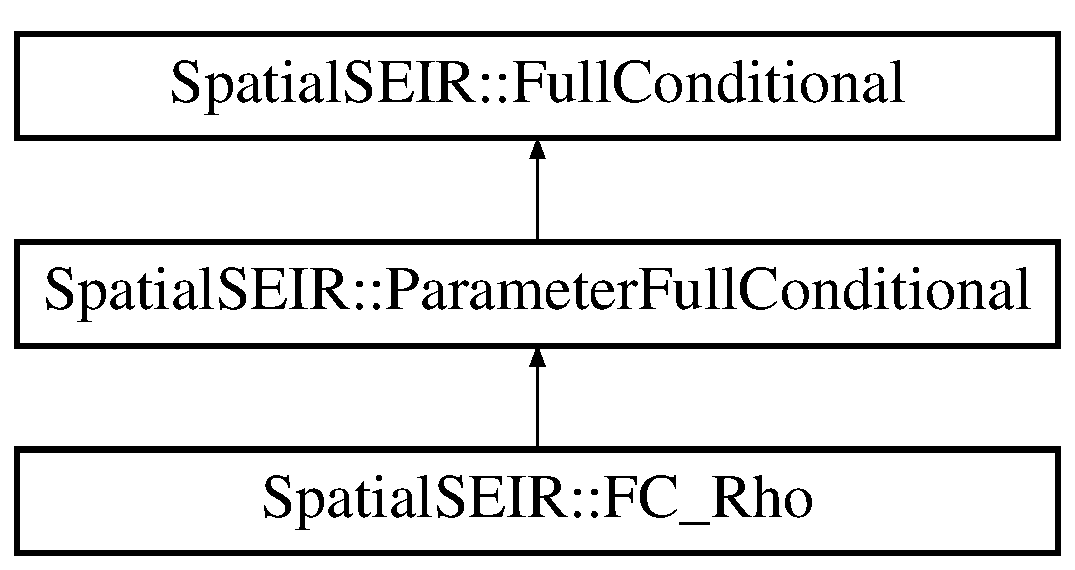
\includegraphics[height=3.000000cm]{classSpatialSEIR_1_1FC__Rho}
\end{center}
\end{figure}
\subsection*{Public Member Functions}
\begin{DoxyCompactItemize}
\item 
\hyperlink{classSpatialSEIR_1_1FC__Rho_abadb39705d3fc20b1a2df40b1cf247b5}{F\-C\-\_\-\-Rho} (\hyperlink{classSpatialSEIR_1_1ModelContext}{Model\-Context} $\ast$\-\_\-context, \hyperlink{classSpatialSEIR_1_1CompartmentalModelMatrix}{Compartmental\-Model\-Matrix} $\ast$\-\_\-\-E\-\_\-star, \hyperlink{classSpatialSEIR_1_1CompartmentalModelMatrix}{Compartmental\-Model\-Matrix} $\ast$\-\_\-\-S, \hyperlink{classSpatialSEIR_1_1InitData}{Init\-Data} $\ast$\-\_\-\-A0, \hyperlink{classSpatialSEIR_1_1CovariateMatrix}{Covariate\-Matrix} $\ast$\-\_\-\-X, double $\ast$\-\_\-p\-\_\-se, double $\ast$\-\_\-beta, double $\ast$\-\_\-rho, double \hyperlink{classSpatialSEIR_1_1FullConditional_a150ee031af8d086ad0a04b13630a110f}{slice\-Width})
\item 
\hyperlink{classSpatialSEIR_1_1FC__Rho_adc75eb5ad6bff0b1cadabb5c86c64a59}{$\sim$\-F\-C\-\_\-\-Rho} ()
\item 
virtual double \hyperlink{classSpatialSEIR_1_1FC__Rho_a8332bf928fd68a2dac08851089a4d527}{eval\-Prior} ()
\item 
virtual int \hyperlink{classSpatialSEIR_1_1FC__Rho_a65e892331f9a129fc5840e7e40af70d4}{eval\-C\-P\-U} ()
\item 
virtual int \hyperlink{classSpatialSEIR_1_1FC__Rho_a918b822d74871547519e5dc62c0bb25f}{eval\-O\-C\-L} ()
\item 
virtual void \hyperlink{classSpatialSEIR_1_1FC__Rho_a0d71fd3e8d9bd120991d60042c3e6a99}{sample} (int verbose)
\item 
virtual long double \hyperlink{classSpatialSEIR_1_1FC__Rho_a2f6ad33590328ce079e7bc9b4f078907}{get\-Value} ()
\item 
virtual void \hyperlink{classSpatialSEIR_1_1FC__Rho_a42dbc09ca0117f10ff27396cddb8dfa8}{set\-Value} (long double val)
\item 
virtual int \hyperlink{classSpatialSEIR_1_1FC__Rho_aaed549dd0c459e96c1697f0578830455}{calculate\-Relevant\-Compartments} ()
\item 
virtual int \hyperlink{classSpatialSEIR_1_1FC__Rho_a676f063fa861ac6297dc18c066bd7cf1}{calculate\-Relevant\-Compartments\-\_\-\-O\-C\-L} ()
\end{DoxyCompactItemize}
\subsection*{Public Attributes}
\begin{DoxyCompactItemize}
\item 
\hyperlink{classSpatialSEIR_1_1ModelContext}{Model\-Context} $\ast$$\ast$ \hyperlink{classSpatialSEIR_1_1FC__Rho_a58528cfb80a3136fdc172a5374598ea9}{context}
\item 
\hyperlink{classSpatialSEIR_1_1CompartmentalModelMatrix}{Compartmental\-Model\-Matrix} $\ast$$\ast$ \hyperlink{classSpatialSEIR_1_1FC__Rho_a5a94d2131584e6eb0519909136fd466d}{E\-\_\-star}
\item 
\hyperlink{classSpatialSEIR_1_1CompartmentalModelMatrix}{Compartmental\-Model\-Matrix} $\ast$$\ast$ \hyperlink{classSpatialSEIR_1_1FC__Rho_a36fc3ffe9ecbcbb68a4cb5810d6cac37}{S}
\item 
\hyperlink{classSpatialSEIR_1_1InitData}{Init\-Data} $\ast$$\ast$ \hyperlink{classSpatialSEIR_1_1FC__Rho_a76cc8299c6cb0159f766fd8d14e8aee7}{A0}
\item 
\hyperlink{classSpatialSEIR_1_1CovariateMatrix}{Covariate\-Matrix} $\ast$$\ast$ \hyperlink{classSpatialSEIR_1_1FC__Rho_a7577871a252d9fe53df7f1f5838bd52e}{X}
\item 
double $\ast$$\ast$ \hyperlink{classSpatialSEIR_1_1FC__Rho_abb3e2be0acefedb35a057590415bd128}{p\-\_\-se}
\item 
double $\ast$$\ast$ \hyperlink{classSpatialSEIR_1_1FC__Rho_a31bd1ce111afce5fc0ac48d1c2a44f53}{beta}
\item 
double $\ast$$\ast$ \hyperlink{classSpatialSEIR_1_1FC__Rho_a26cefbb538d5fe978ad72496d081c5b0}{rho}
\item 
long double $\ast$ \hyperlink{classSpatialSEIR_1_1FC__Rho_a6392b4fa101f7af43ff17f6c8126e5d6}{value}
\end{DoxyCompactItemize}


\subsection{Detailed Description}
\hyperlink{classSpatialSEIR_1_1FC__Rho}{F\-C\-\_\-\-Rho} gives the full conditional distribution of rho, the scalar spatial dependence parameter. 

\subsection{Constructor \& Destructor Documentation}
\hypertarget{classSpatialSEIR_1_1FC__Rho_abadb39705d3fc20b1a2df40b1cf247b5}{\index{Spatial\-S\-E\-I\-R\-::\-F\-C\-\_\-\-Rho@{Spatial\-S\-E\-I\-R\-::\-F\-C\-\_\-\-Rho}!F\-C\-\_\-\-Rho@{F\-C\-\_\-\-Rho}}
\index{F\-C\-\_\-\-Rho@{F\-C\-\_\-\-Rho}!SpatialSEIR::FC_Rho@{Spatial\-S\-E\-I\-R\-::\-F\-C\-\_\-\-Rho}}
\subsubsection[{F\-C\-\_\-\-Rho}]{\setlength{\rightskip}{0pt plus 5cm}Spatial\-S\-E\-I\-R\-::\-F\-C\-\_\-\-Rho\-::\-F\-C\-\_\-\-Rho (
\begin{DoxyParamCaption}
\item[{{\bf Model\-Context} $\ast$}]{\-\_\-context, }
\item[{{\bf Compartmental\-Model\-Matrix} $\ast$}]{\-\_\-\-E\-\_\-star, }
\item[{{\bf Compartmental\-Model\-Matrix} $\ast$}]{\-\_\-\-S, }
\item[{{\bf Init\-Data} $\ast$}]{\-\_\-\-A0, }
\item[{{\bf Covariate\-Matrix} $\ast$}]{\-\_\-\-X, }
\item[{double $\ast$}]{\-\_\-p\-\_\-se, }
\item[{double $\ast$}]{\-\_\-beta, }
\item[{double $\ast$}]{\-\_\-rho, }
\item[{double}]{slice\-Width}
\end{DoxyParamCaption}
)}}\label{classSpatialSEIR_1_1FC__Rho_abadb39705d3fc20b1a2df40b1cf247b5}
\hypertarget{classSpatialSEIR_1_1FC__Rho_adc75eb5ad6bff0b1cadabb5c86c64a59}{\index{Spatial\-S\-E\-I\-R\-::\-F\-C\-\_\-\-Rho@{Spatial\-S\-E\-I\-R\-::\-F\-C\-\_\-\-Rho}!$\sim$\-F\-C\-\_\-\-Rho@{$\sim$\-F\-C\-\_\-\-Rho}}
\index{$\sim$\-F\-C\-\_\-\-Rho@{$\sim$\-F\-C\-\_\-\-Rho}!SpatialSEIR::FC_Rho@{Spatial\-S\-E\-I\-R\-::\-F\-C\-\_\-\-Rho}}
\subsubsection[{$\sim$\-F\-C\-\_\-\-Rho}]{\setlength{\rightskip}{0pt plus 5cm}Spatial\-S\-E\-I\-R\-::\-F\-C\-\_\-\-Rho\-::$\sim$\-F\-C\-\_\-\-Rho (
\begin{DoxyParamCaption}
{}
\end{DoxyParamCaption}
)}}\label{classSpatialSEIR_1_1FC__Rho_adc75eb5ad6bff0b1cadabb5c86c64a59}


\subsection{Member Function Documentation}
\hypertarget{classSpatialSEIR_1_1FC__Rho_aaed549dd0c459e96c1697f0578830455}{\index{Spatial\-S\-E\-I\-R\-::\-F\-C\-\_\-\-Rho@{Spatial\-S\-E\-I\-R\-::\-F\-C\-\_\-\-Rho}!calculate\-Relevant\-Compartments@{calculate\-Relevant\-Compartments}}
\index{calculate\-Relevant\-Compartments@{calculate\-Relevant\-Compartments}!SpatialSEIR::FC_Rho@{Spatial\-S\-E\-I\-R\-::\-F\-C\-\_\-\-Rho}}
\subsubsection[{calculate\-Relevant\-Compartments}]{\setlength{\rightskip}{0pt plus 5cm}int Spatial\-S\-E\-I\-R\-::\-F\-C\-\_\-\-Rho\-::calculate\-Relevant\-Compartments (
\begin{DoxyParamCaption}
{}
\end{DoxyParamCaption}
)\hspace{0.3cm}{\ttfamily [virtual]}}}\label{classSpatialSEIR_1_1FC__Rho_aaed549dd0c459e96c1697f0578830455}


Implements \hyperlink{classSpatialSEIR_1_1ParameterFullConditional_a65c39a2c3ca56e2f194b78cd362d35f9}{Spatial\-S\-E\-I\-R\-::\-Parameter\-Full\-Conditional}.

\hypertarget{classSpatialSEIR_1_1FC__Rho_a676f063fa861ac6297dc18c066bd7cf1}{\index{Spatial\-S\-E\-I\-R\-::\-F\-C\-\_\-\-Rho@{Spatial\-S\-E\-I\-R\-::\-F\-C\-\_\-\-Rho}!calculate\-Relevant\-Compartments\-\_\-\-O\-C\-L@{calculate\-Relevant\-Compartments\-\_\-\-O\-C\-L}}
\index{calculate\-Relevant\-Compartments\-\_\-\-O\-C\-L@{calculate\-Relevant\-Compartments\-\_\-\-O\-C\-L}!SpatialSEIR::FC_Rho@{Spatial\-S\-E\-I\-R\-::\-F\-C\-\_\-\-Rho}}
\subsubsection[{calculate\-Relevant\-Compartments\-\_\-\-O\-C\-L}]{\setlength{\rightskip}{0pt plus 5cm}int Spatial\-S\-E\-I\-R\-::\-F\-C\-\_\-\-Rho\-::calculate\-Relevant\-Compartments\-\_\-\-O\-C\-L (
\begin{DoxyParamCaption}
{}
\end{DoxyParamCaption}
)\hspace{0.3cm}{\ttfamily [virtual]}}}\label{classSpatialSEIR_1_1FC__Rho_a676f063fa861ac6297dc18c066bd7cf1}


Implements \hyperlink{classSpatialSEIR_1_1ParameterFullConditional_af40754537736a64f58848e0368b001fb}{Spatial\-S\-E\-I\-R\-::\-Parameter\-Full\-Conditional}.

\hypertarget{classSpatialSEIR_1_1FC__Rho_a65e892331f9a129fc5840e7e40af70d4}{\index{Spatial\-S\-E\-I\-R\-::\-F\-C\-\_\-\-Rho@{Spatial\-S\-E\-I\-R\-::\-F\-C\-\_\-\-Rho}!eval\-C\-P\-U@{eval\-C\-P\-U}}
\index{eval\-C\-P\-U@{eval\-C\-P\-U}!SpatialSEIR::FC_Rho@{Spatial\-S\-E\-I\-R\-::\-F\-C\-\_\-\-Rho}}
\subsubsection[{eval\-C\-P\-U}]{\setlength{\rightskip}{0pt plus 5cm}int Spatial\-S\-E\-I\-R\-::\-F\-C\-\_\-\-Rho\-::eval\-C\-P\-U (
\begin{DoxyParamCaption}
{}
\end{DoxyParamCaption}
)\hspace{0.3cm}{\ttfamily [virtual]}}}\label{classSpatialSEIR_1_1FC__Rho_a65e892331f9a129fc5840e7e40af70d4}


Implements \hyperlink{classSpatialSEIR_1_1ParameterFullConditional_a186bd19fdeb52ca4522f56fb880201dd}{Spatial\-S\-E\-I\-R\-::\-Parameter\-Full\-Conditional}.

\hypertarget{classSpatialSEIR_1_1FC__Rho_a918b822d74871547519e5dc62c0bb25f}{\index{Spatial\-S\-E\-I\-R\-::\-F\-C\-\_\-\-Rho@{Spatial\-S\-E\-I\-R\-::\-F\-C\-\_\-\-Rho}!eval\-O\-C\-L@{eval\-O\-C\-L}}
\index{eval\-O\-C\-L@{eval\-O\-C\-L}!SpatialSEIR::FC_Rho@{Spatial\-S\-E\-I\-R\-::\-F\-C\-\_\-\-Rho}}
\subsubsection[{eval\-O\-C\-L}]{\setlength{\rightskip}{0pt plus 5cm}int Spatial\-S\-E\-I\-R\-::\-F\-C\-\_\-\-Rho\-::eval\-O\-C\-L (
\begin{DoxyParamCaption}
{}
\end{DoxyParamCaption}
)\hspace{0.3cm}{\ttfamily [virtual]}}}\label{classSpatialSEIR_1_1FC__Rho_a918b822d74871547519e5dc62c0bb25f}


Implements \hyperlink{classSpatialSEIR_1_1ParameterFullConditional_ac4cfb13dace7f72e8136c45d9e959eec}{Spatial\-S\-E\-I\-R\-::\-Parameter\-Full\-Conditional}.

\hypertarget{classSpatialSEIR_1_1FC__Rho_a8332bf928fd68a2dac08851089a4d527}{\index{Spatial\-S\-E\-I\-R\-::\-F\-C\-\_\-\-Rho@{Spatial\-S\-E\-I\-R\-::\-F\-C\-\_\-\-Rho}!eval\-Prior@{eval\-Prior}}
\index{eval\-Prior@{eval\-Prior}!SpatialSEIR::FC_Rho@{Spatial\-S\-E\-I\-R\-::\-F\-C\-\_\-\-Rho}}
\subsubsection[{eval\-Prior}]{\setlength{\rightskip}{0pt plus 5cm}double Spatial\-S\-E\-I\-R\-::\-F\-C\-\_\-\-Rho\-::eval\-Prior (
\begin{DoxyParamCaption}
{}
\end{DoxyParamCaption}
)\hspace{0.3cm}{\ttfamily [virtual]}}}\label{classSpatialSEIR_1_1FC__Rho_a8332bf928fd68a2dac08851089a4d527}
\hypertarget{classSpatialSEIR_1_1FC__Rho_a2f6ad33590328ce079e7bc9b4f078907}{\index{Spatial\-S\-E\-I\-R\-::\-F\-C\-\_\-\-Rho@{Spatial\-S\-E\-I\-R\-::\-F\-C\-\_\-\-Rho}!get\-Value@{get\-Value}}
\index{get\-Value@{get\-Value}!SpatialSEIR::FC_Rho@{Spatial\-S\-E\-I\-R\-::\-F\-C\-\_\-\-Rho}}
\subsubsection[{get\-Value}]{\setlength{\rightskip}{0pt plus 5cm}long double Spatial\-S\-E\-I\-R\-::\-F\-C\-\_\-\-Rho\-::get\-Value (
\begin{DoxyParamCaption}
{}
\end{DoxyParamCaption}
)\hspace{0.3cm}{\ttfamily [virtual]}}}\label{classSpatialSEIR_1_1FC__Rho_a2f6ad33590328ce079e7bc9b4f078907}


Implements \hyperlink{classSpatialSEIR_1_1ParameterFullConditional_a901368d385809e77179b9fa7532adfec}{Spatial\-S\-E\-I\-R\-::\-Parameter\-Full\-Conditional}.

\hypertarget{classSpatialSEIR_1_1FC__Rho_a0d71fd3e8d9bd120991d60042c3e6a99}{\index{Spatial\-S\-E\-I\-R\-::\-F\-C\-\_\-\-Rho@{Spatial\-S\-E\-I\-R\-::\-F\-C\-\_\-\-Rho}!sample@{sample}}
\index{sample@{sample}!SpatialSEIR::FC_Rho@{Spatial\-S\-E\-I\-R\-::\-F\-C\-\_\-\-Rho}}
\subsubsection[{sample}]{\setlength{\rightskip}{0pt plus 5cm}void Spatial\-S\-E\-I\-R\-::\-F\-C\-\_\-\-Rho\-::sample (
\begin{DoxyParamCaption}
\item[{int}]{verbose}
\end{DoxyParamCaption}
)\hspace{0.3cm}{\ttfamily [virtual]}}}\label{classSpatialSEIR_1_1FC__Rho_a0d71fd3e8d9bd120991d60042c3e6a99}


Implements \hyperlink{classSpatialSEIR_1_1ParameterFullConditional_a651e22b15782acb6bd80be12bd476693}{Spatial\-S\-E\-I\-R\-::\-Parameter\-Full\-Conditional}.

\hypertarget{classSpatialSEIR_1_1FC__Rho_a42dbc09ca0117f10ff27396cddb8dfa8}{\index{Spatial\-S\-E\-I\-R\-::\-F\-C\-\_\-\-Rho@{Spatial\-S\-E\-I\-R\-::\-F\-C\-\_\-\-Rho}!set\-Value@{set\-Value}}
\index{set\-Value@{set\-Value}!SpatialSEIR::FC_Rho@{Spatial\-S\-E\-I\-R\-::\-F\-C\-\_\-\-Rho}}
\subsubsection[{set\-Value}]{\setlength{\rightskip}{0pt plus 5cm}void Spatial\-S\-E\-I\-R\-::\-F\-C\-\_\-\-Rho\-::set\-Value (
\begin{DoxyParamCaption}
\item[{long double}]{val}
\end{DoxyParamCaption}
)\hspace{0.3cm}{\ttfamily [virtual]}}}\label{classSpatialSEIR_1_1FC__Rho_a42dbc09ca0117f10ff27396cddb8dfa8}


Implements \hyperlink{classSpatialSEIR_1_1ParameterFullConditional_adf03f213e27d26f120b574d6dd86ffc3}{Spatial\-S\-E\-I\-R\-::\-Parameter\-Full\-Conditional}.



\subsection{Member Data Documentation}
\hypertarget{classSpatialSEIR_1_1FC__Rho_a76cc8299c6cb0159f766fd8d14e8aee7}{\index{Spatial\-S\-E\-I\-R\-::\-F\-C\-\_\-\-Rho@{Spatial\-S\-E\-I\-R\-::\-F\-C\-\_\-\-Rho}!A0@{A0}}
\index{A0@{A0}!SpatialSEIR::FC_Rho@{Spatial\-S\-E\-I\-R\-::\-F\-C\-\_\-\-Rho}}
\subsubsection[{A0}]{\setlength{\rightskip}{0pt plus 5cm}{\bf Init\-Data}$\ast$$\ast$ Spatial\-S\-E\-I\-R\-::\-F\-C\-\_\-\-Rho\-::\-A0}}\label{classSpatialSEIR_1_1FC__Rho_a76cc8299c6cb0159f766fd8d14e8aee7}
\hypertarget{classSpatialSEIR_1_1FC__Rho_a31bd1ce111afce5fc0ac48d1c2a44f53}{\index{Spatial\-S\-E\-I\-R\-::\-F\-C\-\_\-\-Rho@{Spatial\-S\-E\-I\-R\-::\-F\-C\-\_\-\-Rho}!beta@{beta}}
\index{beta@{beta}!SpatialSEIR::FC_Rho@{Spatial\-S\-E\-I\-R\-::\-F\-C\-\_\-\-Rho}}
\subsubsection[{beta}]{\setlength{\rightskip}{0pt plus 5cm}double$\ast$$\ast$ Spatial\-S\-E\-I\-R\-::\-F\-C\-\_\-\-Rho\-::beta}}\label{classSpatialSEIR_1_1FC__Rho_a31bd1ce111afce5fc0ac48d1c2a44f53}
\hypertarget{classSpatialSEIR_1_1FC__Rho_a58528cfb80a3136fdc172a5374598ea9}{\index{Spatial\-S\-E\-I\-R\-::\-F\-C\-\_\-\-Rho@{Spatial\-S\-E\-I\-R\-::\-F\-C\-\_\-\-Rho}!context@{context}}
\index{context@{context}!SpatialSEIR::FC_Rho@{Spatial\-S\-E\-I\-R\-::\-F\-C\-\_\-\-Rho}}
\subsubsection[{context}]{\setlength{\rightskip}{0pt plus 5cm}{\bf Model\-Context}$\ast$$\ast$ Spatial\-S\-E\-I\-R\-::\-F\-C\-\_\-\-Rho\-::context}}\label{classSpatialSEIR_1_1FC__Rho_a58528cfb80a3136fdc172a5374598ea9}
\hypertarget{classSpatialSEIR_1_1FC__Rho_a5a94d2131584e6eb0519909136fd466d}{\index{Spatial\-S\-E\-I\-R\-::\-F\-C\-\_\-\-Rho@{Spatial\-S\-E\-I\-R\-::\-F\-C\-\_\-\-Rho}!E\-\_\-star@{E\-\_\-star}}
\index{E\-\_\-star@{E\-\_\-star}!SpatialSEIR::FC_Rho@{Spatial\-S\-E\-I\-R\-::\-F\-C\-\_\-\-Rho}}
\subsubsection[{E\-\_\-star}]{\setlength{\rightskip}{0pt plus 5cm}{\bf Compartmental\-Model\-Matrix}$\ast$$\ast$ Spatial\-S\-E\-I\-R\-::\-F\-C\-\_\-\-Rho\-::\-E\-\_\-star}}\label{classSpatialSEIR_1_1FC__Rho_a5a94d2131584e6eb0519909136fd466d}
\hypertarget{classSpatialSEIR_1_1FC__Rho_abb3e2be0acefedb35a057590415bd128}{\index{Spatial\-S\-E\-I\-R\-::\-F\-C\-\_\-\-Rho@{Spatial\-S\-E\-I\-R\-::\-F\-C\-\_\-\-Rho}!p\-\_\-se@{p\-\_\-se}}
\index{p\-\_\-se@{p\-\_\-se}!SpatialSEIR::FC_Rho@{Spatial\-S\-E\-I\-R\-::\-F\-C\-\_\-\-Rho}}
\subsubsection[{p\-\_\-se}]{\setlength{\rightskip}{0pt plus 5cm}double$\ast$$\ast$ Spatial\-S\-E\-I\-R\-::\-F\-C\-\_\-\-Rho\-::p\-\_\-se}}\label{classSpatialSEIR_1_1FC__Rho_abb3e2be0acefedb35a057590415bd128}
\hypertarget{classSpatialSEIR_1_1FC__Rho_a26cefbb538d5fe978ad72496d081c5b0}{\index{Spatial\-S\-E\-I\-R\-::\-F\-C\-\_\-\-Rho@{Spatial\-S\-E\-I\-R\-::\-F\-C\-\_\-\-Rho}!rho@{rho}}
\index{rho@{rho}!SpatialSEIR::FC_Rho@{Spatial\-S\-E\-I\-R\-::\-F\-C\-\_\-\-Rho}}
\subsubsection[{rho}]{\setlength{\rightskip}{0pt plus 5cm}double$\ast$$\ast$ Spatial\-S\-E\-I\-R\-::\-F\-C\-\_\-\-Rho\-::rho}}\label{classSpatialSEIR_1_1FC__Rho_a26cefbb538d5fe978ad72496d081c5b0}
\hypertarget{classSpatialSEIR_1_1FC__Rho_a36fc3ffe9ecbcbb68a4cb5810d6cac37}{\index{Spatial\-S\-E\-I\-R\-::\-F\-C\-\_\-\-Rho@{Spatial\-S\-E\-I\-R\-::\-F\-C\-\_\-\-Rho}!S@{S}}
\index{S@{S}!SpatialSEIR::FC_Rho@{Spatial\-S\-E\-I\-R\-::\-F\-C\-\_\-\-Rho}}
\subsubsection[{S}]{\setlength{\rightskip}{0pt plus 5cm}{\bf Compartmental\-Model\-Matrix}$\ast$$\ast$ Spatial\-S\-E\-I\-R\-::\-F\-C\-\_\-\-Rho\-::\-S}}\label{classSpatialSEIR_1_1FC__Rho_a36fc3ffe9ecbcbb68a4cb5810d6cac37}
\hypertarget{classSpatialSEIR_1_1FC__Rho_a6392b4fa101f7af43ff17f6c8126e5d6}{\index{Spatial\-S\-E\-I\-R\-::\-F\-C\-\_\-\-Rho@{Spatial\-S\-E\-I\-R\-::\-F\-C\-\_\-\-Rho}!value@{value}}
\index{value@{value}!SpatialSEIR::FC_Rho@{Spatial\-S\-E\-I\-R\-::\-F\-C\-\_\-\-Rho}}
\subsubsection[{value}]{\setlength{\rightskip}{0pt plus 5cm}long double$\ast$ Spatial\-S\-E\-I\-R\-::\-F\-C\-\_\-\-Rho\-::value}}\label{classSpatialSEIR_1_1FC__Rho_a6392b4fa101f7af43ff17f6c8126e5d6}
\hypertarget{classSpatialSEIR_1_1FC__Rho_a7577871a252d9fe53df7f1f5838bd52e}{\index{Spatial\-S\-E\-I\-R\-::\-F\-C\-\_\-\-Rho@{Spatial\-S\-E\-I\-R\-::\-F\-C\-\_\-\-Rho}!X@{X}}
\index{X@{X}!SpatialSEIR::FC_Rho@{Spatial\-S\-E\-I\-R\-::\-F\-C\-\_\-\-Rho}}
\subsubsection[{X}]{\setlength{\rightskip}{0pt plus 5cm}{\bf Covariate\-Matrix}$\ast$$\ast$ Spatial\-S\-E\-I\-R\-::\-F\-C\-\_\-\-Rho\-::\-X}}\label{classSpatialSEIR_1_1FC__Rho_a7577871a252d9fe53df7f1f5838bd52e}


The documentation for this class was generated from the following files\-:\begin{DoxyCompactItemize}
\item 
lib\-Spatial\-S\-E\-I\-R/include/\-Full\-Conditionals/\hyperlink{LSS__FC__Rho_8hpp}{L\-S\-S\-\_\-\-F\-C\-\_\-\-Rho.\-hpp}\item 
lib\-Spatial\-S\-E\-I\-R/src/\-Full\-Conditionals/\hyperlink{FC__Rho_8cpp}{F\-C\-\_\-\-Rho.\-cpp}\end{DoxyCompactItemize}

\hypertarget{classSpatialSEIR_1_1FC__S0}{\section{Spatial\-S\-E\-I\-R\-:\-:F\-C\-\_\-\-S0 Class Reference}
\label{classSpatialSEIR_1_1FC__S0}\index{Spatial\-S\-E\-I\-R\-::\-F\-C\-\_\-\-S0@{Spatial\-S\-E\-I\-R\-::\-F\-C\-\_\-\-S0}}
}


{\ttfamily \#include $<$L\-S\-S\-\_\-\-F\-C\-\_\-\-S0.\-hpp$>$}

Inheritance diagram for Spatial\-S\-E\-I\-R\-:\-:F\-C\-\_\-\-S0\-:\begin{figure}[H]
\begin{center}
\leavevmode
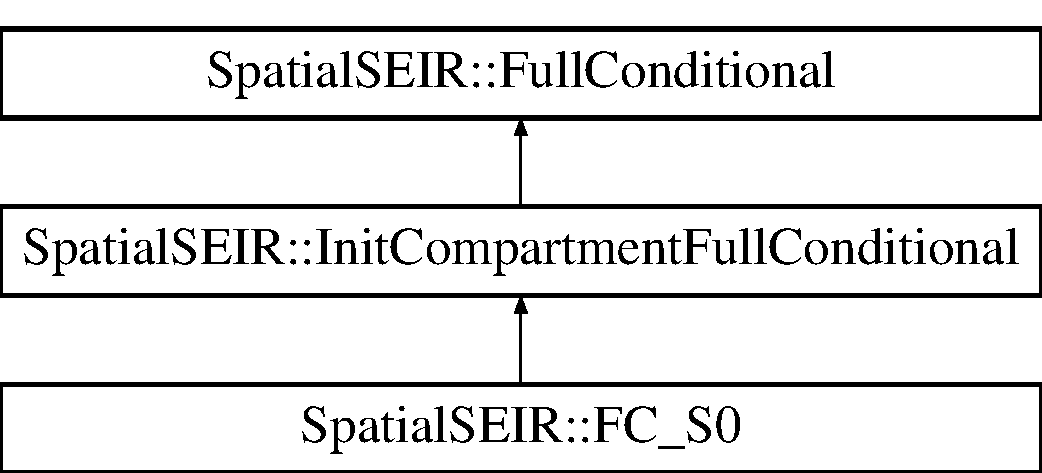
\includegraphics[height=3.000000cm]{classSpatialSEIR_1_1FC__S0}
\end{center}
\end{figure}
\subsection*{Public Member Functions}
\begin{DoxyCompactItemize}
\item 
\hyperlink{classSpatialSEIR_1_1FC__S0_ad1af1632228c5bc1c074c06487ea72de}{F\-C\-\_\-\-S0} (\hyperlink{classSpatialSEIR_1_1ModelContext}{Model\-Context} $\ast$\-\_\-context, \hyperlink{classSpatialSEIR_1_1CompartmentalModelMatrix}{Compartmental\-Model\-Matrix} $\ast$\-\_\-\-S, \hyperlink{classSpatialSEIR_1_1CompartmentalModelMatrix}{Compartmental\-Model\-Matrix} $\ast$\-\_\-\-E, \hyperlink{classSpatialSEIR_1_1CompartmentalModelMatrix}{Compartmental\-Model\-Matrix} $\ast$\-\_\-\-E\-\_\-star, \hyperlink{classSpatialSEIR_1_1CompartmentalModelMatrix}{Compartmental\-Model\-Matrix} $\ast$\-\_\-\-I\-\_\-star, \hyperlink{classSpatialSEIR_1_1InitData}{Init\-Data} $\ast$\-\_\-\-A0, double $\ast$\-\_\-p\-\_\-se, double $\ast$\-\_\-p\-\_\-ei, double \hyperlink{classSpatialSEIR_1_1FullConditional_a150ee031af8d086ad0a04b13630a110f}{slice\-Width})
\item 
virtual \hyperlink{classSpatialSEIR_1_1FC__S0_aa49e31d48cfc1466a86ad50246ffb96c}{$\sim$\-F\-C\-\_\-\-S0} ()
\item 
virtual int \hyperlink{classSpatialSEIR_1_1FC__S0_ae52c137dbd299a31a1b2055e924c93c2}{eval\-C\-P\-U} ()
\item 
virtual int \hyperlink{classSpatialSEIR_1_1FC__S0_a9f9e3df7a26de238959461dd6d2511ef}{eval\-O\-C\-L} ()
\item 
virtual void \hyperlink{classSpatialSEIR_1_1FC__S0_a595cb5eceaa9ede016e1f1d341105de6}{sample} (int verbose)
\item 
virtual long double \hyperlink{classSpatialSEIR_1_1FC__S0_ad1b806dbe3573b1e9652850b934d7b10}{get\-Value} ()
\item 
virtual void \hyperlink{classSpatialSEIR_1_1FC__S0_affd898a5e578d7efec9f133f5031cf13}{set\-Value} (long double \hyperlink{classSpatialSEIR_1_1FC__S0_af2c8815ba97a77505a0851c36dc164f5}{value})
\item 
virtual int \hyperlink{classSpatialSEIR_1_1FC__S0_a755fc8e1d69791f6f3883f12a2f1b1c9}{calculate\-Relevant\-Compartments} ()
\item 
virtual int \hyperlink{classSpatialSEIR_1_1FC__S0_ab1c67b9f867ed1e8b9ac27c4f855a102}{calculate\-Relevant\-Compartments\-\_\-\-O\-C\-L} ()
\end{DoxyCompactItemize}
\subsection*{Public Attributes}
\begin{DoxyCompactItemize}
\item 
\hyperlink{classSpatialSEIR_1_1ModelContext}{Model\-Context} $\ast$$\ast$ \hyperlink{classSpatialSEIR_1_1FC__S0_a83166c2c9ee448358d1e7f2e4984cdc1}{context}
\item 
\hyperlink{classSpatialSEIR_1_1CompartmentalModelMatrix}{Compartmental\-Model\-Matrix} $\ast$$\ast$ \hyperlink{classSpatialSEIR_1_1FC__S0_aaed79f1e5bb2d4b08bc70d1fb71429a9}{S}
\item 
\hyperlink{classSpatialSEIR_1_1CompartmentalModelMatrix}{Compartmental\-Model\-Matrix} $\ast$$\ast$ \hyperlink{classSpatialSEIR_1_1FC__S0_a1ac3fa597eddcde3c6669d823a20c405}{E}
\item 
\hyperlink{classSpatialSEIR_1_1CompartmentalModelMatrix}{Compartmental\-Model\-Matrix} $\ast$$\ast$ \hyperlink{classSpatialSEIR_1_1FC__S0_a4cfa26dfb15450d2a222bcfee37cc35c}{E\-\_\-star}
\item 
\hyperlink{classSpatialSEIR_1_1CompartmentalModelMatrix}{Compartmental\-Model\-Matrix} $\ast$$\ast$ \hyperlink{classSpatialSEIR_1_1FC__S0_a89165d891584534f202f4ecc542bb920}{I\-\_\-star}
\item 
\hyperlink{classSpatialSEIR_1_1InitData}{Init\-Data} $\ast$$\ast$ \hyperlink{classSpatialSEIR_1_1FC__S0_a96ec8ecdc6bd2f9e86122c989e743245}{A0}
\item 
double $\ast$$\ast$ \hyperlink{classSpatialSEIR_1_1FC__S0_a04201525ed952cf56753fdd9a9701596}{p\-\_\-se}
\item 
double $\ast$$\ast$ \hyperlink{classSpatialSEIR_1_1FC__S0_a10210c8d2303327f2ba2646e298e75d4}{p\-\_\-ei}
\item 
long double $\ast$ \hyperlink{classSpatialSEIR_1_1FC__S0_af2c8815ba97a77505a0851c36dc164f5}{value}
\end{DoxyCompactItemize}


\subsection{Detailed Description}
\hyperlink{classSpatialSEIR_1_1FC__S0}{F\-C\-\_\-\-S0} gives the full conditional distribution for the vector of initially susceptible individuals. 

\subsection{Constructor \& Destructor Documentation}
\hypertarget{classSpatialSEIR_1_1FC__S0_ad1af1632228c5bc1c074c06487ea72de}{\index{Spatial\-S\-E\-I\-R\-::\-F\-C\-\_\-\-S0@{Spatial\-S\-E\-I\-R\-::\-F\-C\-\_\-\-S0}!F\-C\-\_\-\-S0@{F\-C\-\_\-\-S0}}
\index{F\-C\-\_\-\-S0@{F\-C\-\_\-\-S0}!SpatialSEIR::FC_S0@{Spatial\-S\-E\-I\-R\-::\-F\-C\-\_\-\-S0}}
\subsubsection[{F\-C\-\_\-\-S0}]{\setlength{\rightskip}{0pt plus 5cm}Spatial\-S\-E\-I\-R\-::\-F\-C\-\_\-\-S0\-::\-F\-C\-\_\-\-S0 (
\begin{DoxyParamCaption}
\item[{{\bf Model\-Context} $\ast$}]{\-\_\-context, }
\item[{{\bf Compartmental\-Model\-Matrix} $\ast$}]{\-\_\-\-S, }
\item[{{\bf Compartmental\-Model\-Matrix} $\ast$}]{\-\_\-\-E, }
\item[{{\bf Compartmental\-Model\-Matrix} $\ast$}]{\-\_\-\-E\-\_\-star, }
\item[{{\bf Compartmental\-Model\-Matrix} $\ast$}]{\-\_\-\-I\-\_\-star, }
\item[{{\bf Init\-Data} $\ast$}]{\-\_\-\-A0, }
\item[{double $\ast$}]{\-\_\-p\-\_\-se, }
\item[{double $\ast$}]{\-\_\-p\-\_\-ei, }
\item[{double}]{slice\-Width}
\end{DoxyParamCaption}
)}}\label{classSpatialSEIR_1_1FC__S0_ad1af1632228c5bc1c074c06487ea72de}
\hypertarget{classSpatialSEIR_1_1FC__S0_aa49e31d48cfc1466a86ad50246ffb96c}{\index{Spatial\-S\-E\-I\-R\-::\-F\-C\-\_\-\-S0@{Spatial\-S\-E\-I\-R\-::\-F\-C\-\_\-\-S0}!$\sim$\-F\-C\-\_\-\-S0@{$\sim$\-F\-C\-\_\-\-S0}}
\index{$\sim$\-F\-C\-\_\-\-S0@{$\sim$\-F\-C\-\_\-\-S0}!SpatialSEIR::FC_S0@{Spatial\-S\-E\-I\-R\-::\-F\-C\-\_\-\-S0}}
\subsubsection[{$\sim$\-F\-C\-\_\-\-S0}]{\setlength{\rightskip}{0pt plus 5cm}Spatial\-S\-E\-I\-R\-::\-F\-C\-\_\-\-S0\-::$\sim$\-F\-C\-\_\-\-S0 (
\begin{DoxyParamCaption}
{}
\end{DoxyParamCaption}
)\hspace{0.3cm}{\ttfamily [virtual]}}}\label{classSpatialSEIR_1_1FC__S0_aa49e31d48cfc1466a86ad50246ffb96c}


\subsection{Member Function Documentation}
\hypertarget{classSpatialSEIR_1_1FC__S0_a755fc8e1d69791f6f3883f12a2f1b1c9}{\index{Spatial\-S\-E\-I\-R\-::\-F\-C\-\_\-\-S0@{Spatial\-S\-E\-I\-R\-::\-F\-C\-\_\-\-S0}!calculate\-Relevant\-Compartments@{calculate\-Relevant\-Compartments}}
\index{calculate\-Relevant\-Compartments@{calculate\-Relevant\-Compartments}!SpatialSEIR::FC_S0@{Spatial\-S\-E\-I\-R\-::\-F\-C\-\_\-\-S0}}
\subsubsection[{calculate\-Relevant\-Compartments}]{\setlength{\rightskip}{0pt plus 5cm}int Spatial\-S\-E\-I\-R\-::\-F\-C\-\_\-\-S0\-::calculate\-Relevant\-Compartments (
\begin{DoxyParamCaption}
{}
\end{DoxyParamCaption}
)\hspace{0.3cm}{\ttfamily [virtual]}}}\label{classSpatialSEIR_1_1FC__S0_a755fc8e1d69791f6f3883f12a2f1b1c9}


Implements \hyperlink{classSpatialSEIR_1_1InitCompartmentFullConditional_a3fab33c4f5b857998fd928a00cea09e7}{Spatial\-S\-E\-I\-R\-::\-Init\-Compartment\-Full\-Conditional}.

\hypertarget{classSpatialSEIR_1_1FC__S0_ab1c67b9f867ed1e8b9ac27c4f855a102}{\index{Spatial\-S\-E\-I\-R\-::\-F\-C\-\_\-\-S0@{Spatial\-S\-E\-I\-R\-::\-F\-C\-\_\-\-S0}!calculate\-Relevant\-Compartments\-\_\-\-O\-C\-L@{calculate\-Relevant\-Compartments\-\_\-\-O\-C\-L}}
\index{calculate\-Relevant\-Compartments\-\_\-\-O\-C\-L@{calculate\-Relevant\-Compartments\-\_\-\-O\-C\-L}!SpatialSEIR::FC_S0@{Spatial\-S\-E\-I\-R\-::\-F\-C\-\_\-\-S0}}
\subsubsection[{calculate\-Relevant\-Compartments\-\_\-\-O\-C\-L}]{\setlength{\rightskip}{0pt plus 5cm}int Spatial\-S\-E\-I\-R\-::\-F\-C\-\_\-\-S0\-::calculate\-Relevant\-Compartments\-\_\-\-O\-C\-L (
\begin{DoxyParamCaption}
{}
\end{DoxyParamCaption}
)\hspace{0.3cm}{\ttfamily [virtual]}}}\label{classSpatialSEIR_1_1FC__S0_ab1c67b9f867ed1e8b9ac27c4f855a102}


Implements \hyperlink{classSpatialSEIR_1_1InitCompartmentFullConditional_aa4eae1aafbcdc4819be2e520d600dedf}{Spatial\-S\-E\-I\-R\-::\-Init\-Compartment\-Full\-Conditional}.

\hypertarget{classSpatialSEIR_1_1FC__S0_ae52c137dbd299a31a1b2055e924c93c2}{\index{Spatial\-S\-E\-I\-R\-::\-F\-C\-\_\-\-S0@{Spatial\-S\-E\-I\-R\-::\-F\-C\-\_\-\-S0}!eval\-C\-P\-U@{eval\-C\-P\-U}}
\index{eval\-C\-P\-U@{eval\-C\-P\-U}!SpatialSEIR::FC_S0@{Spatial\-S\-E\-I\-R\-::\-F\-C\-\_\-\-S0}}
\subsubsection[{eval\-C\-P\-U}]{\setlength{\rightskip}{0pt plus 5cm}int Spatial\-S\-E\-I\-R\-::\-F\-C\-\_\-\-S0\-::eval\-C\-P\-U (
\begin{DoxyParamCaption}
{}
\end{DoxyParamCaption}
)\hspace{0.3cm}{\ttfamily [virtual]}}}\label{classSpatialSEIR_1_1FC__S0_ae52c137dbd299a31a1b2055e924c93c2}


Implements \hyperlink{classSpatialSEIR_1_1InitCompartmentFullConditional_a25fc6e3ac2cb71a6e115ce3235fd8de0}{Spatial\-S\-E\-I\-R\-::\-Init\-Compartment\-Full\-Conditional}.

\hypertarget{classSpatialSEIR_1_1FC__S0_a9f9e3df7a26de238959461dd6d2511ef}{\index{Spatial\-S\-E\-I\-R\-::\-F\-C\-\_\-\-S0@{Spatial\-S\-E\-I\-R\-::\-F\-C\-\_\-\-S0}!eval\-O\-C\-L@{eval\-O\-C\-L}}
\index{eval\-O\-C\-L@{eval\-O\-C\-L}!SpatialSEIR::FC_S0@{Spatial\-S\-E\-I\-R\-::\-F\-C\-\_\-\-S0}}
\subsubsection[{eval\-O\-C\-L}]{\setlength{\rightskip}{0pt plus 5cm}int Spatial\-S\-E\-I\-R\-::\-F\-C\-\_\-\-S0\-::eval\-O\-C\-L (
\begin{DoxyParamCaption}
{}
\end{DoxyParamCaption}
)\hspace{0.3cm}{\ttfamily [virtual]}}}\label{classSpatialSEIR_1_1FC__S0_a9f9e3df7a26de238959461dd6d2511ef}


Implements \hyperlink{classSpatialSEIR_1_1InitCompartmentFullConditional_a2f0c4b5628e2f2074c1a84ea6349a754}{Spatial\-S\-E\-I\-R\-::\-Init\-Compartment\-Full\-Conditional}.

\hypertarget{classSpatialSEIR_1_1FC__S0_ad1b806dbe3573b1e9652850b934d7b10}{\index{Spatial\-S\-E\-I\-R\-::\-F\-C\-\_\-\-S0@{Spatial\-S\-E\-I\-R\-::\-F\-C\-\_\-\-S0}!get\-Value@{get\-Value}}
\index{get\-Value@{get\-Value}!SpatialSEIR::FC_S0@{Spatial\-S\-E\-I\-R\-::\-F\-C\-\_\-\-S0}}
\subsubsection[{get\-Value}]{\setlength{\rightskip}{0pt plus 5cm}long double Spatial\-S\-E\-I\-R\-::\-F\-C\-\_\-\-S0\-::get\-Value (
\begin{DoxyParamCaption}
{}
\end{DoxyParamCaption}
)\hspace{0.3cm}{\ttfamily [virtual]}}}\label{classSpatialSEIR_1_1FC__S0_ad1b806dbe3573b1e9652850b934d7b10}


Implements \hyperlink{classSpatialSEIR_1_1InitCompartmentFullConditional_aadb3975a791221136e6c4be5e016d9f1}{Spatial\-S\-E\-I\-R\-::\-Init\-Compartment\-Full\-Conditional}.

\hypertarget{classSpatialSEIR_1_1FC__S0_a595cb5eceaa9ede016e1f1d341105de6}{\index{Spatial\-S\-E\-I\-R\-::\-F\-C\-\_\-\-S0@{Spatial\-S\-E\-I\-R\-::\-F\-C\-\_\-\-S0}!sample@{sample}}
\index{sample@{sample}!SpatialSEIR::FC_S0@{Spatial\-S\-E\-I\-R\-::\-F\-C\-\_\-\-S0}}
\subsubsection[{sample}]{\setlength{\rightskip}{0pt plus 5cm}void Spatial\-S\-E\-I\-R\-::\-F\-C\-\_\-\-S0\-::sample (
\begin{DoxyParamCaption}
\item[{int}]{verbose}
\end{DoxyParamCaption}
)\hspace{0.3cm}{\ttfamily [virtual]}}}\label{classSpatialSEIR_1_1FC__S0_a595cb5eceaa9ede016e1f1d341105de6}


Implements \hyperlink{classSpatialSEIR_1_1InitCompartmentFullConditional_a03bcc440fa87265336980f3e833f59f2}{Spatial\-S\-E\-I\-R\-::\-Init\-Compartment\-Full\-Conditional}.

\hypertarget{classSpatialSEIR_1_1FC__S0_affd898a5e578d7efec9f133f5031cf13}{\index{Spatial\-S\-E\-I\-R\-::\-F\-C\-\_\-\-S0@{Spatial\-S\-E\-I\-R\-::\-F\-C\-\_\-\-S0}!set\-Value@{set\-Value}}
\index{set\-Value@{set\-Value}!SpatialSEIR::FC_S0@{Spatial\-S\-E\-I\-R\-::\-F\-C\-\_\-\-S0}}
\subsubsection[{set\-Value}]{\setlength{\rightskip}{0pt plus 5cm}void Spatial\-S\-E\-I\-R\-::\-F\-C\-\_\-\-S0\-::set\-Value (
\begin{DoxyParamCaption}
\item[{long double}]{value}
\end{DoxyParamCaption}
)\hspace{0.3cm}{\ttfamily [virtual]}}}\label{classSpatialSEIR_1_1FC__S0_affd898a5e578d7efec9f133f5031cf13}


Implements \hyperlink{classSpatialSEIR_1_1InitCompartmentFullConditional_acbc03a68f5c67beacefadcc3c22c1d88}{Spatial\-S\-E\-I\-R\-::\-Init\-Compartment\-Full\-Conditional}.



\subsection{Member Data Documentation}
\hypertarget{classSpatialSEIR_1_1FC__S0_a96ec8ecdc6bd2f9e86122c989e743245}{\index{Spatial\-S\-E\-I\-R\-::\-F\-C\-\_\-\-S0@{Spatial\-S\-E\-I\-R\-::\-F\-C\-\_\-\-S0}!A0@{A0}}
\index{A0@{A0}!SpatialSEIR::FC_S0@{Spatial\-S\-E\-I\-R\-::\-F\-C\-\_\-\-S0}}
\subsubsection[{A0}]{\setlength{\rightskip}{0pt plus 5cm}{\bf Init\-Data}$\ast$$\ast$ Spatial\-S\-E\-I\-R\-::\-F\-C\-\_\-\-S0\-::\-A0}}\label{classSpatialSEIR_1_1FC__S0_a96ec8ecdc6bd2f9e86122c989e743245}
\hypertarget{classSpatialSEIR_1_1FC__S0_a83166c2c9ee448358d1e7f2e4984cdc1}{\index{Spatial\-S\-E\-I\-R\-::\-F\-C\-\_\-\-S0@{Spatial\-S\-E\-I\-R\-::\-F\-C\-\_\-\-S0}!context@{context}}
\index{context@{context}!SpatialSEIR::FC_S0@{Spatial\-S\-E\-I\-R\-::\-F\-C\-\_\-\-S0}}
\subsubsection[{context}]{\setlength{\rightskip}{0pt plus 5cm}{\bf Model\-Context}$\ast$$\ast$ Spatial\-S\-E\-I\-R\-::\-F\-C\-\_\-\-S0\-::context}}\label{classSpatialSEIR_1_1FC__S0_a83166c2c9ee448358d1e7f2e4984cdc1}
\hypertarget{classSpatialSEIR_1_1FC__S0_a1ac3fa597eddcde3c6669d823a20c405}{\index{Spatial\-S\-E\-I\-R\-::\-F\-C\-\_\-\-S0@{Spatial\-S\-E\-I\-R\-::\-F\-C\-\_\-\-S0}!E@{E}}
\index{E@{E}!SpatialSEIR::FC_S0@{Spatial\-S\-E\-I\-R\-::\-F\-C\-\_\-\-S0}}
\subsubsection[{E}]{\setlength{\rightskip}{0pt plus 5cm}{\bf Compartmental\-Model\-Matrix}$\ast$$\ast$ Spatial\-S\-E\-I\-R\-::\-F\-C\-\_\-\-S0\-::\-E}}\label{classSpatialSEIR_1_1FC__S0_a1ac3fa597eddcde3c6669d823a20c405}
\hypertarget{classSpatialSEIR_1_1FC__S0_a4cfa26dfb15450d2a222bcfee37cc35c}{\index{Spatial\-S\-E\-I\-R\-::\-F\-C\-\_\-\-S0@{Spatial\-S\-E\-I\-R\-::\-F\-C\-\_\-\-S0}!E\-\_\-star@{E\-\_\-star}}
\index{E\-\_\-star@{E\-\_\-star}!SpatialSEIR::FC_S0@{Spatial\-S\-E\-I\-R\-::\-F\-C\-\_\-\-S0}}
\subsubsection[{E\-\_\-star}]{\setlength{\rightskip}{0pt plus 5cm}{\bf Compartmental\-Model\-Matrix}$\ast$$\ast$ Spatial\-S\-E\-I\-R\-::\-F\-C\-\_\-\-S0\-::\-E\-\_\-star}}\label{classSpatialSEIR_1_1FC__S0_a4cfa26dfb15450d2a222bcfee37cc35c}
\hypertarget{classSpatialSEIR_1_1FC__S0_a89165d891584534f202f4ecc542bb920}{\index{Spatial\-S\-E\-I\-R\-::\-F\-C\-\_\-\-S0@{Spatial\-S\-E\-I\-R\-::\-F\-C\-\_\-\-S0}!I\-\_\-star@{I\-\_\-star}}
\index{I\-\_\-star@{I\-\_\-star}!SpatialSEIR::FC_S0@{Spatial\-S\-E\-I\-R\-::\-F\-C\-\_\-\-S0}}
\subsubsection[{I\-\_\-star}]{\setlength{\rightskip}{0pt plus 5cm}{\bf Compartmental\-Model\-Matrix}$\ast$$\ast$ Spatial\-S\-E\-I\-R\-::\-F\-C\-\_\-\-S0\-::\-I\-\_\-star}}\label{classSpatialSEIR_1_1FC__S0_a89165d891584534f202f4ecc542bb920}
\hypertarget{classSpatialSEIR_1_1FC__S0_a10210c8d2303327f2ba2646e298e75d4}{\index{Spatial\-S\-E\-I\-R\-::\-F\-C\-\_\-\-S0@{Spatial\-S\-E\-I\-R\-::\-F\-C\-\_\-\-S0}!p\-\_\-ei@{p\-\_\-ei}}
\index{p\-\_\-ei@{p\-\_\-ei}!SpatialSEIR::FC_S0@{Spatial\-S\-E\-I\-R\-::\-F\-C\-\_\-\-S0}}
\subsubsection[{p\-\_\-ei}]{\setlength{\rightskip}{0pt plus 5cm}double$\ast$$\ast$ Spatial\-S\-E\-I\-R\-::\-F\-C\-\_\-\-S0\-::p\-\_\-ei}}\label{classSpatialSEIR_1_1FC__S0_a10210c8d2303327f2ba2646e298e75d4}
\hypertarget{classSpatialSEIR_1_1FC__S0_a04201525ed952cf56753fdd9a9701596}{\index{Spatial\-S\-E\-I\-R\-::\-F\-C\-\_\-\-S0@{Spatial\-S\-E\-I\-R\-::\-F\-C\-\_\-\-S0}!p\-\_\-se@{p\-\_\-se}}
\index{p\-\_\-se@{p\-\_\-se}!SpatialSEIR::FC_S0@{Spatial\-S\-E\-I\-R\-::\-F\-C\-\_\-\-S0}}
\subsubsection[{p\-\_\-se}]{\setlength{\rightskip}{0pt plus 5cm}double$\ast$$\ast$ Spatial\-S\-E\-I\-R\-::\-F\-C\-\_\-\-S0\-::p\-\_\-se}}\label{classSpatialSEIR_1_1FC__S0_a04201525ed952cf56753fdd9a9701596}
\hypertarget{classSpatialSEIR_1_1FC__S0_aaed79f1e5bb2d4b08bc70d1fb71429a9}{\index{Spatial\-S\-E\-I\-R\-::\-F\-C\-\_\-\-S0@{Spatial\-S\-E\-I\-R\-::\-F\-C\-\_\-\-S0}!S@{S}}
\index{S@{S}!SpatialSEIR::FC_S0@{Spatial\-S\-E\-I\-R\-::\-F\-C\-\_\-\-S0}}
\subsubsection[{S}]{\setlength{\rightskip}{0pt plus 5cm}{\bf Compartmental\-Model\-Matrix}$\ast$$\ast$ Spatial\-S\-E\-I\-R\-::\-F\-C\-\_\-\-S0\-::\-S}}\label{classSpatialSEIR_1_1FC__S0_aaed79f1e5bb2d4b08bc70d1fb71429a9}
\hypertarget{classSpatialSEIR_1_1FC__S0_af2c8815ba97a77505a0851c36dc164f5}{\index{Spatial\-S\-E\-I\-R\-::\-F\-C\-\_\-\-S0@{Spatial\-S\-E\-I\-R\-::\-F\-C\-\_\-\-S0}!value@{value}}
\index{value@{value}!SpatialSEIR::FC_S0@{Spatial\-S\-E\-I\-R\-::\-F\-C\-\_\-\-S0}}
\subsubsection[{value}]{\setlength{\rightskip}{0pt plus 5cm}long double$\ast$ Spatial\-S\-E\-I\-R\-::\-F\-C\-\_\-\-S0\-::value}}\label{classSpatialSEIR_1_1FC__S0_af2c8815ba97a77505a0851c36dc164f5}


The documentation for this class was generated from the following files\-:\begin{DoxyCompactItemize}
\item 
lib\-Spatial\-S\-E\-I\-R/include/\-Full\-Conditionals/\hyperlink{LSS__FC__S0_8hpp}{L\-S\-S\-\_\-\-F\-C\-\_\-\-S0.\-hpp}\item 
lib\-Spatial\-S\-E\-I\-R/src/\-Full\-Conditionals/\hyperlink{FC__S0_8cpp}{F\-C\-\_\-\-S0.\-cpp}\end{DoxyCompactItemize}

\hypertarget{classSpatialSEIR_1_1FC__S__Star}{\section{Spatial\-S\-E\-I\-R\-:\-:F\-C\-\_\-\-S\-\_\-\-Star Class Reference}
\label{classSpatialSEIR_1_1FC__S__Star}\index{Spatial\-S\-E\-I\-R\-::\-F\-C\-\_\-\-S\-\_\-\-Star@{Spatial\-S\-E\-I\-R\-::\-F\-C\-\_\-\-S\-\_\-\-Star}}
}


{\ttfamily \#include $<$L\-S\-S\-\_\-\-F\-C\-\_\-\-S\-\_\-star.\-hpp$>$}

Inheritance diagram for Spatial\-S\-E\-I\-R\-:\-:F\-C\-\_\-\-S\-\_\-\-Star\-:\begin{figure}[H]
\begin{center}
\leavevmode
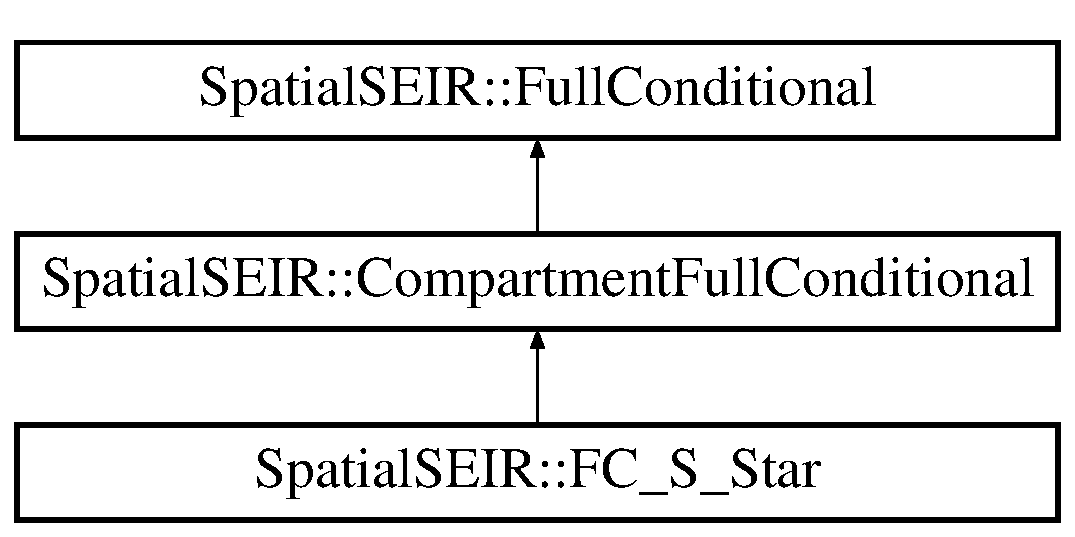
\includegraphics[height=3.000000cm]{classSpatialSEIR_1_1FC__S__Star}
\end{center}
\end{figure}
\subsection*{Public Member Functions}
\begin{DoxyCompactItemize}
\item 
\hyperlink{classSpatialSEIR_1_1FC__S__Star_a080c77a634e28265cbc33e08ad2ea8d9}{F\-C\-\_\-\-S\-\_\-\-Star} (\hyperlink{classSpatialSEIR_1_1ModelContext}{Model\-Context} $\ast$\-\_\-context, \hyperlink{classSpatialSEIR_1_1CompartmentalModelMatrix}{Compartmental\-Model\-Matrix} $\ast$\-\_\-\-S\-\_\-star, \hyperlink{classSpatialSEIR_1_1CompartmentalModelMatrix}{Compartmental\-Model\-Matrix} $\ast$\-\_\-\-S, \hyperlink{classSpatialSEIR_1_1CompartmentalModelMatrix}{Compartmental\-Model\-Matrix} $\ast$\-\_\-\-R, \hyperlink{classSpatialSEIR_1_1CompartmentalModelMatrix}{Compartmental\-Model\-Matrix} $\ast$\-\_\-\-E\-\_\-star, \hyperlink{classSpatialSEIR_1_1CompartmentalModelMatrix}{Compartmental\-Model\-Matrix} $\ast$\-\_\-\-R\-\_\-star, \hyperlink{classSpatialSEIR_1_1InitData}{Init\-Data} $\ast$\-\_\-\-A0, \hyperlink{classSpatialSEIR_1_1CovariateMatrix}{Covariate\-Matrix} $\ast$\-\_\-\-X, double $\ast$\-\_\-p\-\_\-se, double $\ast$\-\_\-p\-\_\-rs, double $\ast$\-\_\-beta, double $\ast$\-\_\-rho, double \-\_\-steady\-State\-Constraint\-Precision, double \hyperlink{classSpatialSEIR_1_1FullConditional_a150ee031af8d086ad0a04b13630a110f}{slice\-Width})
\item 
virtual int \hyperlink{classSpatialSEIR_1_1FC__S__Star_a85f440e1a945be994cbbdcbafca9d125}{eval\-C\-P\-U} ()
\item 
virtual int \hyperlink{classSpatialSEIR_1_1FC__S__Star_aaa438f0eae4ff7ac24721a5e4eb67ac3}{eval\-C\-P\-U} (int i, int j)
\item 
virtual int \hyperlink{classSpatialSEIR_1_1FC__S__Star_a36db3b203873bca03bbd5d6d52fc55d5}{eval\-O\-C\-L} ()
\item 
virtual void \hyperlink{classSpatialSEIR_1_1FC__S__Star_acf2c800d9bed70b302b8ec7c1dd9358f}{sample} (int verbose)
\item 
virtual long double \hyperlink{classSpatialSEIR_1_1FC__S__Star_a3dd725f1ab193c0b0774c498be092344}{get\-Value} ()
\item 
virtual void \hyperlink{classSpatialSEIR_1_1FC__S__Star_a1d86c5a35b1e626124b05aafdd5b87fa}{set\-Value} (long double val)
\item 
virtual int \hyperlink{classSpatialSEIR_1_1FC__S__Star_a0059f6af650ff4d0e5bfc17a3a4a6f0c}{calculate\-Relevant\-Compartments} ()
\item 
virtual int \hyperlink{classSpatialSEIR_1_1FC__S__Star_a2caf261df37f0b20d2ded6630332886c}{calculate\-Relevant\-Compartments} (int i, int j)
\item 
virtual int \hyperlink{classSpatialSEIR_1_1FC__S__Star_aca332563eafecfb7f7d85b61c87ceb15}{calculate\-Relevant\-Compartments\-\_\-\-O\-C\-L} ()
\item 
virtual \hyperlink{classSpatialSEIR_1_1FC__S__Star_ab48460dbce4e3e9eb35233f3a1ea8313}{$\sim$\-F\-C\-\_\-\-S\-\_\-\-Star} ()
\end{DoxyCompactItemize}
\subsection*{Public Attributes}
\begin{DoxyCompactItemize}
\item 
\hyperlink{classSpatialSEIR_1_1ModelContext}{Model\-Context} $\ast$$\ast$ \hyperlink{classSpatialSEIR_1_1FC__S__Star_a5b90884aaea81dcdd1828b01c06b3e43}{context}
\item 
\hyperlink{classSpatialSEIR_1_1CompartmentalModelMatrix}{Compartmental\-Model\-Matrix} $\ast$$\ast$ \hyperlink{classSpatialSEIR_1_1FC__S__Star_ae7955695f611091c04fcc01d721d6225}{S\-\_\-star}
\item 
\hyperlink{classSpatialSEIR_1_1CompartmentalModelMatrix}{Compartmental\-Model\-Matrix} $\ast$$\ast$ \hyperlink{classSpatialSEIR_1_1FC__S__Star_ad49b3322944c04467da8f9a50bfe8554}{S}
\item 
\hyperlink{classSpatialSEIR_1_1CompartmentalModelMatrix}{Compartmental\-Model\-Matrix} $\ast$$\ast$ \hyperlink{classSpatialSEIR_1_1FC__S__Star_a0fb9730dc4cfdcaeaf8dd7f1254d2e93}{R}
\item 
\hyperlink{classSpatialSEIR_1_1CompartmentalModelMatrix}{Compartmental\-Model\-Matrix} $\ast$$\ast$ \hyperlink{classSpatialSEIR_1_1FC__S__Star_a98b5975a91f1e27f089a19910bf030ee}{E\-\_\-star}
\item 
\hyperlink{classSpatialSEIR_1_1CompartmentalModelMatrix}{Compartmental\-Model\-Matrix} $\ast$$\ast$ \hyperlink{classSpatialSEIR_1_1FC__S__Star_a3b09aa8e732a12af5bbae9c0c48da242}{R\-\_\-star}
\item 
\hyperlink{classSpatialSEIR_1_1InitData}{Init\-Data} $\ast$$\ast$ \hyperlink{classSpatialSEIR_1_1FC__S__Star_adb3257cc96f16d56589ad96cc74d0ab7}{A0}
\item 
\hyperlink{classSpatialSEIR_1_1CovariateMatrix}{Covariate\-Matrix} $\ast$$\ast$ \hyperlink{classSpatialSEIR_1_1FC__S__Star_a46f078abec44ca9708b65a8ab402ddb7}{X}
\item 
double $\ast$$\ast$ \hyperlink{classSpatialSEIR_1_1FC__S__Star_aed0125c2ef3ac758f046b7b8dea44697}{p\-\_\-se}
\item 
double $\ast$$\ast$ \hyperlink{classSpatialSEIR_1_1FC__S__Star_afa71439e5a1928e50266d7f8b066bd88}{p\-\_\-rs}
\item 
double $\ast$$\ast$ \hyperlink{classSpatialSEIR_1_1FC__S__Star_a1a588918ec2011729fde87d46cbc22ec}{beta}
\item 
double $\ast$$\ast$ \hyperlink{classSpatialSEIR_1_1FC__S__Star_a7477bcae8127617f68b081e8ccb2a38b}{rho}
\item 
long double $\ast$ \hyperlink{classSpatialSEIR_1_1FC__S__Star_a92c36f1dc6a099c072ffe591c3ceac2c}{value}
\item 
double $\ast$ \hyperlink{classSpatialSEIR_1_1FC__S__Star_ad49895014dd714807c7fb4b3fe6b86cc}{steady\-State\-Constraint\-Precision}
\end{DoxyCompactItemize}


\subsection{Detailed Description}
\hyperlink{classSpatialSEIR_1_1FC__S__Star}{F\-C\-\_\-\-S\-\_\-\-Star} gives the full conditional distribution of S\-\_\-star, the transition matrix capturing individuals moving from the removed/recovered category to the susceptible category. 

\subsection{Constructor \& Destructor Documentation}
\hypertarget{classSpatialSEIR_1_1FC__S__Star_a080c77a634e28265cbc33e08ad2ea8d9}{\index{Spatial\-S\-E\-I\-R\-::\-F\-C\-\_\-\-S\-\_\-\-Star@{Spatial\-S\-E\-I\-R\-::\-F\-C\-\_\-\-S\-\_\-\-Star}!F\-C\-\_\-\-S\-\_\-\-Star@{F\-C\-\_\-\-S\-\_\-\-Star}}
\index{F\-C\-\_\-\-S\-\_\-\-Star@{F\-C\-\_\-\-S\-\_\-\-Star}!SpatialSEIR::FC_S_Star@{Spatial\-S\-E\-I\-R\-::\-F\-C\-\_\-\-S\-\_\-\-Star}}
\subsubsection[{F\-C\-\_\-\-S\-\_\-\-Star}]{\setlength{\rightskip}{0pt plus 5cm}Spatial\-S\-E\-I\-R\-::\-F\-C\-\_\-\-S\-\_\-\-Star\-::\-F\-C\-\_\-\-S\-\_\-\-Star (
\begin{DoxyParamCaption}
\item[{{\bf Model\-Context} $\ast$}]{\-\_\-context, }
\item[{{\bf Compartmental\-Model\-Matrix} $\ast$}]{\-\_\-\-S\-\_\-star, }
\item[{{\bf Compartmental\-Model\-Matrix} $\ast$}]{\-\_\-\-S, }
\item[{{\bf Compartmental\-Model\-Matrix} $\ast$}]{\-\_\-\-R, }
\item[{{\bf Compartmental\-Model\-Matrix} $\ast$}]{\-\_\-\-E\-\_\-star, }
\item[{{\bf Compartmental\-Model\-Matrix} $\ast$}]{\-\_\-\-R\-\_\-star, }
\item[{{\bf Init\-Data} $\ast$}]{\-\_\-\-A0, }
\item[{{\bf Covariate\-Matrix} $\ast$}]{\-\_\-\-X, }
\item[{double $\ast$}]{\-\_\-p\-\_\-se, }
\item[{double $\ast$}]{\-\_\-p\-\_\-rs, }
\item[{double $\ast$}]{\-\_\-beta, }
\item[{double $\ast$}]{\-\_\-rho, }
\item[{double}]{\-\_\-steady\-State\-Constraint\-Precision, }
\item[{double}]{slice\-Width}
\end{DoxyParamCaption}
)}}\label{classSpatialSEIR_1_1FC__S__Star_a080c77a634e28265cbc33e08ad2ea8d9}
\hypertarget{classSpatialSEIR_1_1FC__S__Star_ab48460dbce4e3e9eb35233f3a1ea8313}{\index{Spatial\-S\-E\-I\-R\-::\-F\-C\-\_\-\-S\-\_\-\-Star@{Spatial\-S\-E\-I\-R\-::\-F\-C\-\_\-\-S\-\_\-\-Star}!$\sim$\-F\-C\-\_\-\-S\-\_\-\-Star@{$\sim$\-F\-C\-\_\-\-S\-\_\-\-Star}}
\index{$\sim$\-F\-C\-\_\-\-S\-\_\-\-Star@{$\sim$\-F\-C\-\_\-\-S\-\_\-\-Star}!SpatialSEIR::FC_S_Star@{Spatial\-S\-E\-I\-R\-::\-F\-C\-\_\-\-S\-\_\-\-Star}}
\subsubsection[{$\sim$\-F\-C\-\_\-\-S\-\_\-\-Star}]{\setlength{\rightskip}{0pt plus 5cm}Spatial\-S\-E\-I\-R\-::\-F\-C\-\_\-\-S\-\_\-\-Star\-::$\sim$\-F\-C\-\_\-\-S\-\_\-\-Star (
\begin{DoxyParamCaption}
{}
\end{DoxyParamCaption}
)\hspace{0.3cm}{\ttfamily [virtual]}}}\label{classSpatialSEIR_1_1FC__S__Star_ab48460dbce4e3e9eb35233f3a1ea8313}


\subsection{Member Function Documentation}
\hypertarget{classSpatialSEIR_1_1FC__S__Star_a0059f6af650ff4d0e5bfc17a3a4a6f0c}{\index{Spatial\-S\-E\-I\-R\-::\-F\-C\-\_\-\-S\-\_\-\-Star@{Spatial\-S\-E\-I\-R\-::\-F\-C\-\_\-\-S\-\_\-\-Star}!calculate\-Relevant\-Compartments@{calculate\-Relevant\-Compartments}}
\index{calculate\-Relevant\-Compartments@{calculate\-Relevant\-Compartments}!SpatialSEIR::FC_S_Star@{Spatial\-S\-E\-I\-R\-::\-F\-C\-\_\-\-S\-\_\-\-Star}}
\subsubsection[{calculate\-Relevant\-Compartments}]{\setlength{\rightskip}{0pt plus 5cm}int Spatial\-S\-E\-I\-R\-::\-F\-C\-\_\-\-S\-\_\-\-Star\-::calculate\-Relevant\-Compartments (
\begin{DoxyParamCaption}
{}
\end{DoxyParamCaption}
)\hspace{0.3cm}{\ttfamily [virtual]}}}\label{classSpatialSEIR_1_1FC__S__Star_a0059f6af650ff4d0e5bfc17a3a4a6f0c}


Implements \hyperlink{classSpatialSEIR_1_1CompartmentFullConditional_a71836271b0997117f3b8437c2f55a986}{Spatial\-S\-E\-I\-R\-::\-Compartment\-Full\-Conditional}.

\hypertarget{classSpatialSEIR_1_1FC__S__Star_a2caf261df37f0b20d2ded6630332886c}{\index{Spatial\-S\-E\-I\-R\-::\-F\-C\-\_\-\-S\-\_\-\-Star@{Spatial\-S\-E\-I\-R\-::\-F\-C\-\_\-\-S\-\_\-\-Star}!calculate\-Relevant\-Compartments@{calculate\-Relevant\-Compartments}}
\index{calculate\-Relevant\-Compartments@{calculate\-Relevant\-Compartments}!SpatialSEIR::FC_S_Star@{Spatial\-S\-E\-I\-R\-::\-F\-C\-\_\-\-S\-\_\-\-Star}}
\subsubsection[{calculate\-Relevant\-Compartments}]{\setlength{\rightskip}{0pt plus 5cm}int Spatial\-S\-E\-I\-R\-::\-F\-C\-\_\-\-S\-\_\-\-Star\-::calculate\-Relevant\-Compartments (
\begin{DoxyParamCaption}
\item[{int}]{i, }
\item[{int}]{j}
\end{DoxyParamCaption}
)\hspace{0.3cm}{\ttfamily [virtual]}}}\label{classSpatialSEIR_1_1FC__S__Star_a2caf261df37f0b20d2ded6630332886c}


Implements \hyperlink{classSpatialSEIR_1_1CompartmentFullConditional_a21440bf07bd554a2893a328713bfe09f}{Spatial\-S\-E\-I\-R\-::\-Compartment\-Full\-Conditional}.

\hypertarget{classSpatialSEIR_1_1FC__S__Star_aca332563eafecfb7f7d85b61c87ceb15}{\index{Spatial\-S\-E\-I\-R\-::\-F\-C\-\_\-\-S\-\_\-\-Star@{Spatial\-S\-E\-I\-R\-::\-F\-C\-\_\-\-S\-\_\-\-Star}!calculate\-Relevant\-Compartments\-\_\-\-O\-C\-L@{calculate\-Relevant\-Compartments\-\_\-\-O\-C\-L}}
\index{calculate\-Relevant\-Compartments\-\_\-\-O\-C\-L@{calculate\-Relevant\-Compartments\-\_\-\-O\-C\-L}!SpatialSEIR::FC_S_Star@{Spatial\-S\-E\-I\-R\-::\-F\-C\-\_\-\-S\-\_\-\-Star}}
\subsubsection[{calculate\-Relevant\-Compartments\-\_\-\-O\-C\-L}]{\setlength{\rightskip}{0pt plus 5cm}int Spatial\-S\-E\-I\-R\-::\-F\-C\-\_\-\-S\-\_\-\-Star\-::calculate\-Relevant\-Compartments\-\_\-\-O\-C\-L (
\begin{DoxyParamCaption}
{}
\end{DoxyParamCaption}
)\hspace{0.3cm}{\ttfamily [virtual]}}}\label{classSpatialSEIR_1_1FC__S__Star_aca332563eafecfb7f7d85b61c87ceb15}


Implements \hyperlink{classSpatialSEIR_1_1CompartmentFullConditional_ab873ecc59f7639637113d885ab89bed4}{Spatial\-S\-E\-I\-R\-::\-Compartment\-Full\-Conditional}.

\hypertarget{classSpatialSEIR_1_1FC__S__Star_a85f440e1a945be994cbbdcbafca9d125}{\index{Spatial\-S\-E\-I\-R\-::\-F\-C\-\_\-\-S\-\_\-\-Star@{Spatial\-S\-E\-I\-R\-::\-F\-C\-\_\-\-S\-\_\-\-Star}!eval\-C\-P\-U@{eval\-C\-P\-U}}
\index{eval\-C\-P\-U@{eval\-C\-P\-U}!SpatialSEIR::FC_S_Star@{Spatial\-S\-E\-I\-R\-::\-F\-C\-\_\-\-S\-\_\-\-Star}}
\subsubsection[{eval\-C\-P\-U}]{\setlength{\rightskip}{0pt plus 5cm}int Spatial\-S\-E\-I\-R\-::\-F\-C\-\_\-\-S\-\_\-\-Star\-::eval\-C\-P\-U (
\begin{DoxyParamCaption}
{}
\end{DoxyParamCaption}
)\hspace{0.3cm}{\ttfamily [virtual]}}}\label{classSpatialSEIR_1_1FC__S__Star_a85f440e1a945be994cbbdcbafca9d125}


Implements \hyperlink{classSpatialSEIR_1_1CompartmentFullConditional_ad2402c8d7fc0b362482bcd5ceaa035af}{Spatial\-S\-E\-I\-R\-::\-Compartment\-Full\-Conditional}.

\hypertarget{classSpatialSEIR_1_1FC__S__Star_aaa438f0eae4ff7ac24721a5e4eb67ac3}{\index{Spatial\-S\-E\-I\-R\-::\-F\-C\-\_\-\-S\-\_\-\-Star@{Spatial\-S\-E\-I\-R\-::\-F\-C\-\_\-\-S\-\_\-\-Star}!eval\-C\-P\-U@{eval\-C\-P\-U}}
\index{eval\-C\-P\-U@{eval\-C\-P\-U}!SpatialSEIR::FC_S_Star@{Spatial\-S\-E\-I\-R\-::\-F\-C\-\_\-\-S\-\_\-\-Star}}
\subsubsection[{eval\-C\-P\-U}]{\setlength{\rightskip}{0pt plus 5cm}int Spatial\-S\-E\-I\-R\-::\-F\-C\-\_\-\-S\-\_\-\-Star\-::eval\-C\-P\-U (
\begin{DoxyParamCaption}
\item[{int}]{i, }
\item[{int}]{j}
\end{DoxyParamCaption}
)\hspace{0.3cm}{\ttfamily [virtual]}}}\label{classSpatialSEIR_1_1FC__S__Star_aaa438f0eae4ff7ac24721a5e4eb67ac3}


Implements \hyperlink{classSpatialSEIR_1_1CompartmentFullConditional_a92d48bc8cd13ff048791edbdcc453479}{Spatial\-S\-E\-I\-R\-::\-Compartment\-Full\-Conditional}.

\hypertarget{classSpatialSEIR_1_1FC__S__Star_a36db3b203873bca03bbd5d6d52fc55d5}{\index{Spatial\-S\-E\-I\-R\-::\-F\-C\-\_\-\-S\-\_\-\-Star@{Spatial\-S\-E\-I\-R\-::\-F\-C\-\_\-\-S\-\_\-\-Star}!eval\-O\-C\-L@{eval\-O\-C\-L}}
\index{eval\-O\-C\-L@{eval\-O\-C\-L}!SpatialSEIR::FC_S_Star@{Spatial\-S\-E\-I\-R\-::\-F\-C\-\_\-\-S\-\_\-\-Star}}
\subsubsection[{eval\-O\-C\-L}]{\setlength{\rightskip}{0pt plus 5cm}int Spatial\-S\-E\-I\-R\-::\-F\-C\-\_\-\-S\-\_\-\-Star\-::eval\-O\-C\-L (
\begin{DoxyParamCaption}
{}
\end{DoxyParamCaption}
)\hspace{0.3cm}{\ttfamily [virtual]}}}\label{classSpatialSEIR_1_1FC__S__Star_a36db3b203873bca03bbd5d6d52fc55d5}


Implements \hyperlink{classSpatialSEIR_1_1CompartmentFullConditional_ac7c7b1191508d49a56ec739449bf93d4}{Spatial\-S\-E\-I\-R\-::\-Compartment\-Full\-Conditional}.

\hypertarget{classSpatialSEIR_1_1FC__S__Star_a3dd725f1ab193c0b0774c498be092344}{\index{Spatial\-S\-E\-I\-R\-::\-F\-C\-\_\-\-S\-\_\-\-Star@{Spatial\-S\-E\-I\-R\-::\-F\-C\-\_\-\-S\-\_\-\-Star}!get\-Value@{get\-Value}}
\index{get\-Value@{get\-Value}!SpatialSEIR::FC_S_Star@{Spatial\-S\-E\-I\-R\-::\-F\-C\-\_\-\-S\-\_\-\-Star}}
\subsubsection[{get\-Value}]{\setlength{\rightskip}{0pt plus 5cm}long double Spatial\-S\-E\-I\-R\-::\-F\-C\-\_\-\-S\-\_\-\-Star\-::get\-Value (
\begin{DoxyParamCaption}
{}
\end{DoxyParamCaption}
)\hspace{0.3cm}{\ttfamily [virtual]}}}\label{classSpatialSEIR_1_1FC__S__Star_a3dd725f1ab193c0b0774c498be092344}


Implements \hyperlink{classSpatialSEIR_1_1CompartmentFullConditional_a28794be23ee7f6fcba96ff2bee63e065}{Spatial\-S\-E\-I\-R\-::\-Compartment\-Full\-Conditional}.

\hypertarget{classSpatialSEIR_1_1FC__S__Star_acf2c800d9bed70b302b8ec7c1dd9358f}{\index{Spatial\-S\-E\-I\-R\-::\-F\-C\-\_\-\-S\-\_\-\-Star@{Spatial\-S\-E\-I\-R\-::\-F\-C\-\_\-\-S\-\_\-\-Star}!sample@{sample}}
\index{sample@{sample}!SpatialSEIR::FC_S_Star@{Spatial\-S\-E\-I\-R\-::\-F\-C\-\_\-\-S\-\_\-\-Star}}
\subsubsection[{sample}]{\setlength{\rightskip}{0pt plus 5cm}void Spatial\-S\-E\-I\-R\-::\-F\-C\-\_\-\-S\-\_\-\-Star\-::sample (
\begin{DoxyParamCaption}
\item[{int}]{verbose}
\end{DoxyParamCaption}
)\hspace{0.3cm}{\ttfamily [virtual]}}}\label{classSpatialSEIR_1_1FC__S__Star_acf2c800d9bed70b302b8ec7c1dd9358f}


Implements \hyperlink{classSpatialSEIR_1_1CompartmentFullConditional_a436ae9e47f7a4269f0a78ce225e6b7f3}{Spatial\-S\-E\-I\-R\-::\-Compartment\-Full\-Conditional}.

\hypertarget{classSpatialSEIR_1_1FC__S__Star_a1d86c5a35b1e626124b05aafdd5b87fa}{\index{Spatial\-S\-E\-I\-R\-::\-F\-C\-\_\-\-S\-\_\-\-Star@{Spatial\-S\-E\-I\-R\-::\-F\-C\-\_\-\-S\-\_\-\-Star}!set\-Value@{set\-Value}}
\index{set\-Value@{set\-Value}!SpatialSEIR::FC_S_Star@{Spatial\-S\-E\-I\-R\-::\-F\-C\-\_\-\-S\-\_\-\-Star}}
\subsubsection[{set\-Value}]{\setlength{\rightskip}{0pt plus 5cm}void Spatial\-S\-E\-I\-R\-::\-F\-C\-\_\-\-S\-\_\-\-Star\-::set\-Value (
\begin{DoxyParamCaption}
\item[{long double}]{val}
\end{DoxyParamCaption}
)\hspace{0.3cm}{\ttfamily [virtual]}}}\label{classSpatialSEIR_1_1FC__S__Star_a1d86c5a35b1e626124b05aafdd5b87fa}


Implements \hyperlink{classSpatialSEIR_1_1CompartmentFullConditional_a22ab4dcc354c8ebc4f619685bc32dfae}{Spatial\-S\-E\-I\-R\-::\-Compartment\-Full\-Conditional}.



\subsection{Member Data Documentation}
\hypertarget{classSpatialSEIR_1_1FC__S__Star_adb3257cc96f16d56589ad96cc74d0ab7}{\index{Spatial\-S\-E\-I\-R\-::\-F\-C\-\_\-\-S\-\_\-\-Star@{Spatial\-S\-E\-I\-R\-::\-F\-C\-\_\-\-S\-\_\-\-Star}!A0@{A0}}
\index{A0@{A0}!SpatialSEIR::FC_S_Star@{Spatial\-S\-E\-I\-R\-::\-F\-C\-\_\-\-S\-\_\-\-Star}}
\subsubsection[{A0}]{\setlength{\rightskip}{0pt plus 5cm}{\bf Init\-Data}$\ast$$\ast$ Spatial\-S\-E\-I\-R\-::\-F\-C\-\_\-\-S\-\_\-\-Star\-::\-A0}}\label{classSpatialSEIR_1_1FC__S__Star_adb3257cc96f16d56589ad96cc74d0ab7}
\hypertarget{classSpatialSEIR_1_1FC__S__Star_a1a588918ec2011729fde87d46cbc22ec}{\index{Spatial\-S\-E\-I\-R\-::\-F\-C\-\_\-\-S\-\_\-\-Star@{Spatial\-S\-E\-I\-R\-::\-F\-C\-\_\-\-S\-\_\-\-Star}!beta@{beta}}
\index{beta@{beta}!SpatialSEIR::FC_S_Star@{Spatial\-S\-E\-I\-R\-::\-F\-C\-\_\-\-S\-\_\-\-Star}}
\subsubsection[{beta}]{\setlength{\rightskip}{0pt plus 5cm}double$\ast$$\ast$ Spatial\-S\-E\-I\-R\-::\-F\-C\-\_\-\-S\-\_\-\-Star\-::beta}}\label{classSpatialSEIR_1_1FC__S__Star_a1a588918ec2011729fde87d46cbc22ec}
\hypertarget{classSpatialSEIR_1_1FC__S__Star_a5b90884aaea81dcdd1828b01c06b3e43}{\index{Spatial\-S\-E\-I\-R\-::\-F\-C\-\_\-\-S\-\_\-\-Star@{Spatial\-S\-E\-I\-R\-::\-F\-C\-\_\-\-S\-\_\-\-Star}!context@{context}}
\index{context@{context}!SpatialSEIR::FC_S_Star@{Spatial\-S\-E\-I\-R\-::\-F\-C\-\_\-\-S\-\_\-\-Star}}
\subsubsection[{context}]{\setlength{\rightskip}{0pt plus 5cm}{\bf Model\-Context}$\ast$$\ast$ Spatial\-S\-E\-I\-R\-::\-F\-C\-\_\-\-S\-\_\-\-Star\-::context}}\label{classSpatialSEIR_1_1FC__S__Star_a5b90884aaea81dcdd1828b01c06b3e43}
\hypertarget{classSpatialSEIR_1_1FC__S__Star_a98b5975a91f1e27f089a19910bf030ee}{\index{Spatial\-S\-E\-I\-R\-::\-F\-C\-\_\-\-S\-\_\-\-Star@{Spatial\-S\-E\-I\-R\-::\-F\-C\-\_\-\-S\-\_\-\-Star}!E\-\_\-star@{E\-\_\-star}}
\index{E\-\_\-star@{E\-\_\-star}!SpatialSEIR::FC_S_Star@{Spatial\-S\-E\-I\-R\-::\-F\-C\-\_\-\-S\-\_\-\-Star}}
\subsubsection[{E\-\_\-star}]{\setlength{\rightskip}{0pt plus 5cm}{\bf Compartmental\-Model\-Matrix}$\ast$$\ast$ Spatial\-S\-E\-I\-R\-::\-F\-C\-\_\-\-S\-\_\-\-Star\-::\-E\-\_\-star}}\label{classSpatialSEIR_1_1FC__S__Star_a98b5975a91f1e27f089a19910bf030ee}
\hypertarget{classSpatialSEIR_1_1FC__S__Star_afa71439e5a1928e50266d7f8b066bd88}{\index{Spatial\-S\-E\-I\-R\-::\-F\-C\-\_\-\-S\-\_\-\-Star@{Spatial\-S\-E\-I\-R\-::\-F\-C\-\_\-\-S\-\_\-\-Star}!p\-\_\-rs@{p\-\_\-rs}}
\index{p\-\_\-rs@{p\-\_\-rs}!SpatialSEIR::FC_S_Star@{Spatial\-S\-E\-I\-R\-::\-F\-C\-\_\-\-S\-\_\-\-Star}}
\subsubsection[{p\-\_\-rs}]{\setlength{\rightskip}{0pt plus 5cm}double$\ast$$\ast$ Spatial\-S\-E\-I\-R\-::\-F\-C\-\_\-\-S\-\_\-\-Star\-::p\-\_\-rs}}\label{classSpatialSEIR_1_1FC__S__Star_afa71439e5a1928e50266d7f8b066bd88}
\hypertarget{classSpatialSEIR_1_1FC__S__Star_aed0125c2ef3ac758f046b7b8dea44697}{\index{Spatial\-S\-E\-I\-R\-::\-F\-C\-\_\-\-S\-\_\-\-Star@{Spatial\-S\-E\-I\-R\-::\-F\-C\-\_\-\-S\-\_\-\-Star}!p\-\_\-se@{p\-\_\-se}}
\index{p\-\_\-se@{p\-\_\-se}!SpatialSEIR::FC_S_Star@{Spatial\-S\-E\-I\-R\-::\-F\-C\-\_\-\-S\-\_\-\-Star}}
\subsubsection[{p\-\_\-se}]{\setlength{\rightskip}{0pt plus 5cm}double$\ast$$\ast$ Spatial\-S\-E\-I\-R\-::\-F\-C\-\_\-\-S\-\_\-\-Star\-::p\-\_\-se}}\label{classSpatialSEIR_1_1FC__S__Star_aed0125c2ef3ac758f046b7b8dea44697}
\hypertarget{classSpatialSEIR_1_1FC__S__Star_a0fb9730dc4cfdcaeaf8dd7f1254d2e93}{\index{Spatial\-S\-E\-I\-R\-::\-F\-C\-\_\-\-S\-\_\-\-Star@{Spatial\-S\-E\-I\-R\-::\-F\-C\-\_\-\-S\-\_\-\-Star}!R@{R}}
\index{R@{R}!SpatialSEIR::FC_S_Star@{Spatial\-S\-E\-I\-R\-::\-F\-C\-\_\-\-S\-\_\-\-Star}}
\subsubsection[{R}]{\setlength{\rightskip}{0pt plus 5cm}{\bf Compartmental\-Model\-Matrix}$\ast$$\ast$ Spatial\-S\-E\-I\-R\-::\-F\-C\-\_\-\-S\-\_\-\-Star\-::\-R}}\label{classSpatialSEIR_1_1FC__S__Star_a0fb9730dc4cfdcaeaf8dd7f1254d2e93}
\hypertarget{classSpatialSEIR_1_1FC__S__Star_a3b09aa8e732a12af5bbae9c0c48da242}{\index{Spatial\-S\-E\-I\-R\-::\-F\-C\-\_\-\-S\-\_\-\-Star@{Spatial\-S\-E\-I\-R\-::\-F\-C\-\_\-\-S\-\_\-\-Star}!R\-\_\-star@{R\-\_\-star}}
\index{R\-\_\-star@{R\-\_\-star}!SpatialSEIR::FC_S_Star@{Spatial\-S\-E\-I\-R\-::\-F\-C\-\_\-\-S\-\_\-\-Star}}
\subsubsection[{R\-\_\-star}]{\setlength{\rightskip}{0pt plus 5cm}{\bf Compartmental\-Model\-Matrix}$\ast$$\ast$ Spatial\-S\-E\-I\-R\-::\-F\-C\-\_\-\-S\-\_\-\-Star\-::\-R\-\_\-star}}\label{classSpatialSEIR_1_1FC__S__Star_a3b09aa8e732a12af5bbae9c0c48da242}
\hypertarget{classSpatialSEIR_1_1FC__S__Star_a7477bcae8127617f68b081e8ccb2a38b}{\index{Spatial\-S\-E\-I\-R\-::\-F\-C\-\_\-\-S\-\_\-\-Star@{Spatial\-S\-E\-I\-R\-::\-F\-C\-\_\-\-S\-\_\-\-Star}!rho@{rho}}
\index{rho@{rho}!SpatialSEIR::FC_S_Star@{Spatial\-S\-E\-I\-R\-::\-F\-C\-\_\-\-S\-\_\-\-Star}}
\subsubsection[{rho}]{\setlength{\rightskip}{0pt plus 5cm}double$\ast$$\ast$ Spatial\-S\-E\-I\-R\-::\-F\-C\-\_\-\-S\-\_\-\-Star\-::rho}}\label{classSpatialSEIR_1_1FC__S__Star_a7477bcae8127617f68b081e8ccb2a38b}
\hypertarget{classSpatialSEIR_1_1FC__S__Star_ad49b3322944c04467da8f9a50bfe8554}{\index{Spatial\-S\-E\-I\-R\-::\-F\-C\-\_\-\-S\-\_\-\-Star@{Spatial\-S\-E\-I\-R\-::\-F\-C\-\_\-\-S\-\_\-\-Star}!S@{S}}
\index{S@{S}!SpatialSEIR::FC_S_Star@{Spatial\-S\-E\-I\-R\-::\-F\-C\-\_\-\-S\-\_\-\-Star}}
\subsubsection[{S}]{\setlength{\rightskip}{0pt plus 5cm}{\bf Compartmental\-Model\-Matrix}$\ast$$\ast$ Spatial\-S\-E\-I\-R\-::\-F\-C\-\_\-\-S\-\_\-\-Star\-::\-S}}\label{classSpatialSEIR_1_1FC__S__Star_ad49b3322944c04467da8f9a50bfe8554}
\hypertarget{classSpatialSEIR_1_1FC__S__Star_ae7955695f611091c04fcc01d721d6225}{\index{Spatial\-S\-E\-I\-R\-::\-F\-C\-\_\-\-S\-\_\-\-Star@{Spatial\-S\-E\-I\-R\-::\-F\-C\-\_\-\-S\-\_\-\-Star}!S\-\_\-star@{S\-\_\-star}}
\index{S\-\_\-star@{S\-\_\-star}!SpatialSEIR::FC_S_Star@{Spatial\-S\-E\-I\-R\-::\-F\-C\-\_\-\-S\-\_\-\-Star}}
\subsubsection[{S\-\_\-star}]{\setlength{\rightskip}{0pt plus 5cm}{\bf Compartmental\-Model\-Matrix}$\ast$$\ast$ Spatial\-S\-E\-I\-R\-::\-F\-C\-\_\-\-S\-\_\-\-Star\-::\-S\-\_\-star}}\label{classSpatialSEIR_1_1FC__S__Star_ae7955695f611091c04fcc01d721d6225}
\hypertarget{classSpatialSEIR_1_1FC__S__Star_ad49895014dd714807c7fb4b3fe6b86cc}{\index{Spatial\-S\-E\-I\-R\-::\-F\-C\-\_\-\-S\-\_\-\-Star@{Spatial\-S\-E\-I\-R\-::\-F\-C\-\_\-\-S\-\_\-\-Star}!steady\-State\-Constraint\-Precision@{steady\-State\-Constraint\-Precision}}
\index{steady\-State\-Constraint\-Precision@{steady\-State\-Constraint\-Precision}!SpatialSEIR::FC_S_Star@{Spatial\-S\-E\-I\-R\-::\-F\-C\-\_\-\-S\-\_\-\-Star}}
\subsubsection[{steady\-State\-Constraint\-Precision}]{\setlength{\rightskip}{0pt plus 5cm}double$\ast$ Spatial\-S\-E\-I\-R\-::\-F\-C\-\_\-\-S\-\_\-\-Star\-::steady\-State\-Constraint\-Precision}}\label{classSpatialSEIR_1_1FC__S__Star_ad49895014dd714807c7fb4b3fe6b86cc}
\hypertarget{classSpatialSEIR_1_1FC__S__Star_a92c36f1dc6a099c072ffe591c3ceac2c}{\index{Spatial\-S\-E\-I\-R\-::\-F\-C\-\_\-\-S\-\_\-\-Star@{Spatial\-S\-E\-I\-R\-::\-F\-C\-\_\-\-S\-\_\-\-Star}!value@{value}}
\index{value@{value}!SpatialSEIR::FC_S_Star@{Spatial\-S\-E\-I\-R\-::\-F\-C\-\_\-\-S\-\_\-\-Star}}
\subsubsection[{value}]{\setlength{\rightskip}{0pt plus 5cm}long double$\ast$ Spatial\-S\-E\-I\-R\-::\-F\-C\-\_\-\-S\-\_\-\-Star\-::value}}\label{classSpatialSEIR_1_1FC__S__Star_a92c36f1dc6a099c072ffe591c3ceac2c}
\hypertarget{classSpatialSEIR_1_1FC__S__Star_a46f078abec44ca9708b65a8ab402ddb7}{\index{Spatial\-S\-E\-I\-R\-::\-F\-C\-\_\-\-S\-\_\-\-Star@{Spatial\-S\-E\-I\-R\-::\-F\-C\-\_\-\-S\-\_\-\-Star}!X@{X}}
\index{X@{X}!SpatialSEIR::FC_S_Star@{Spatial\-S\-E\-I\-R\-::\-F\-C\-\_\-\-S\-\_\-\-Star}}
\subsubsection[{X}]{\setlength{\rightskip}{0pt plus 5cm}{\bf Covariate\-Matrix}$\ast$$\ast$ Spatial\-S\-E\-I\-R\-::\-F\-C\-\_\-\-S\-\_\-\-Star\-::\-X}}\label{classSpatialSEIR_1_1FC__S__Star_a46f078abec44ca9708b65a8ab402ddb7}


The documentation for this class was generated from the following files\-:\begin{DoxyCompactItemize}
\item 
lib\-Spatial\-S\-E\-I\-R/include/\-Full\-Conditionals/\hyperlink{LSS__FC__S__star_8hpp}{L\-S\-S\-\_\-\-F\-C\-\_\-\-S\-\_\-star.\-hpp}\item 
lib\-Spatial\-S\-E\-I\-R/src/\-Full\-Conditionals/\hyperlink{FC__S__star_8cpp}{F\-C\-\_\-\-S\-\_\-star.\-cpp}\end{DoxyCompactItemize}

\hypertarget{classSpatialSEIR_1_1FullConditional}{\section{Spatial\-S\-E\-I\-R\-:\-:Full\-Conditional Class Reference}
\label{classSpatialSEIR_1_1FullConditional}\index{Spatial\-S\-E\-I\-R\-::\-Full\-Conditional@{Spatial\-S\-E\-I\-R\-::\-Full\-Conditional}}
}


{\ttfamily \#include $<$L\-S\-S\-\_\-\-Full\-Conditional.\-hpp$>$}

Inheritance diagram for Spatial\-S\-E\-I\-R\-:\-:Full\-Conditional\-:\begin{figure}[H]
\begin{center}
\leavevmode
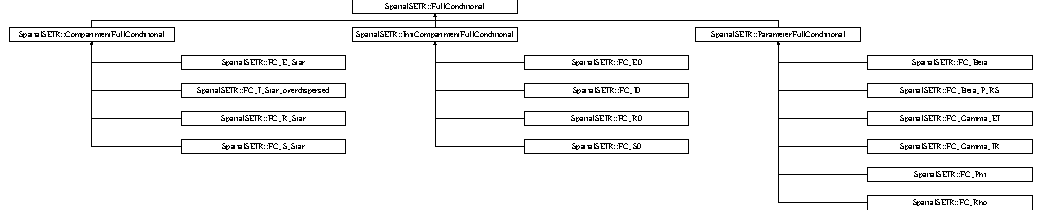
\includegraphics[height=2.828283cm]{classSpatialSEIR_1_1FullConditional}
\end{center}
\end{figure}
\subsection*{Public Member Functions}
\begin{DoxyCompactItemize}
\item 
virtual \hyperlink{classSpatialSEIR_1_1FullConditional_ae3c3cbadab4183ba85f530471bf175c2}{$\sim$\-Full\-Conditional} ()
\item 
virtual void \hyperlink{classSpatialSEIR_1_1FullConditional_aac6928c9c2753acfc2c9e9bbe840ba82}{sample} (int verbose)=0
\item 
virtual long double \hyperlink{classSpatialSEIR_1_1FullConditional_abe67c774a66370686ee9dc6fe6f278f6}{get\-Value} ()=0
\item 
virtual void \hyperlink{classSpatialSEIR_1_1FullConditional_a0834b0bb81ef4f7f368ba87fd784ff39}{set\-Value} (long double value)=0
\item 
virtual int \hyperlink{classSpatialSEIR_1_1FullConditional_a04c671e900a359f5a554817f21a99b5c}{calculate\-Relevant\-Compartments} ()=0
\item 
virtual int \hyperlink{classSpatialSEIR_1_1FullConditional_a77b75e8e1f62175aa0380a2e9aca3d46}{calculate\-Relevant\-Compartments\-\_\-\-O\-C\-L} ()=0
\item 
virtual void \hyperlink{classSpatialSEIR_1_1FullConditional_afd84b9273d641028453aefc06b342782}{update\-Sampling\-Parameters} (double desired\-Ratio, double target\-Width, double proportion\-Change)=0
\item 
virtual int \hyperlink{classSpatialSEIR_1_1FullConditional_a680a2a8af1962a5a99191ff84acf78c5}{get\-Full\-Conditional\-Type} ()=0
\item 
double \hyperlink{classSpatialSEIR_1_1FullConditional_ad9074ca43ff07ee923f08ac0fbf46cc1}{acceptance\-Ratio} ()
\item 
void \hyperlink{classSpatialSEIR_1_1FullConditional_a5aa519fb2a20d3f694890e2d1ab7da48}{set\-Sampler\-Type} (int type)
\end{DoxyCompactItemize}
\subsection*{Public Attributes}
\begin{DoxyCompactItemize}
\item 
double $\ast$ \hyperlink{classSpatialSEIR_1_1FullConditional_a150ee031af8d086ad0a04b13630a110f}{slice\-Width}
\item 
std\-::vector$<$ \hyperlink{classSpatialSEIR_1_1Sampler}{Sampler} $\ast$ $>$ $\ast$ \hyperlink{classSpatialSEIR_1_1FullConditional_ad6801b12eafd9a487f93f832d5873b23}{samplers}
\item 
\hyperlink{classSpatialSEIR_1_1Sampler}{Sampler} $\ast$$\ast$ \hyperlink{classSpatialSEIR_1_1FullConditional_a051095c43d42bd08d6f2318c51135aab}{current\-Sampler}
\item 
int $\ast$ \hyperlink{classSpatialSEIR_1_1FullConditional_ad76bbf21e116bf68a323aea46b57d7dd}{samples}
\item 
int $\ast$ \hyperlink{classSpatialSEIR_1_1FullConditional_ac2305c4de13aeb0206ce293fb689692b}{accepted}
\end{DoxyCompactItemize}


\subsection{Detailed Description}
The \hyperlink{classSpatialSEIR_1_1FullConditional}{Full\-Conditional} class serves as the grandparent class for the various full conditional distributions. This structure is helpful, because we can then implement general methods which apply to all child classes of \hyperlink{classSpatialSEIR_1_1FullConditional}{Full\-Conditional}. 

\subsection{Constructor \& Destructor Documentation}
\hypertarget{classSpatialSEIR_1_1FullConditional_ae3c3cbadab4183ba85f530471bf175c2}{\index{Spatial\-S\-E\-I\-R\-::\-Full\-Conditional@{Spatial\-S\-E\-I\-R\-::\-Full\-Conditional}!$\sim$\-Full\-Conditional@{$\sim$\-Full\-Conditional}}
\index{$\sim$\-Full\-Conditional@{$\sim$\-Full\-Conditional}!SpatialSEIR::FullConditional@{Spatial\-S\-E\-I\-R\-::\-Full\-Conditional}}
\subsubsection[{$\sim$\-Full\-Conditional}]{\setlength{\rightskip}{0pt plus 5cm}virtual Spatial\-S\-E\-I\-R\-::\-Full\-Conditional\-::$\sim$\-Full\-Conditional (
\begin{DoxyParamCaption}
{}
\end{DoxyParamCaption}
)\hspace{0.3cm}{\ttfamily [inline]}, {\ttfamily [virtual]}}}\label{classSpatialSEIR_1_1FullConditional_ae3c3cbadab4183ba85f530471bf175c2}


\subsection{Member Function Documentation}
\hypertarget{classSpatialSEIR_1_1FullConditional_ad9074ca43ff07ee923f08ac0fbf46cc1}{\index{Spatial\-S\-E\-I\-R\-::\-Full\-Conditional@{Spatial\-S\-E\-I\-R\-::\-Full\-Conditional}!acceptance\-Ratio@{acceptance\-Ratio}}
\index{acceptance\-Ratio@{acceptance\-Ratio}!SpatialSEIR::FullConditional@{Spatial\-S\-E\-I\-R\-::\-Full\-Conditional}}
\subsubsection[{acceptance\-Ratio}]{\setlength{\rightskip}{0pt plus 5cm}double Spatial\-S\-E\-I\-R\-::\-Full\-Conditional\-::acceptance\-Ratio (
\begin{DoxyParamCaption}
{}
\end{DoxyParamCaption}
)}}\label{classSpatialSEIR_1_1FullConditional_ad9074ca43ff07ee923f08ac0fbf46cc1}
\hypertarget{classSpatialSEIR_1_1FullConditional_a04c671e900a359f5a554817f21a99b5c}{\index{Spatial\-S\-E\-I\-R\-::\-Full\-Conditional@{Spatial\-S\-E\-I\-R\-::\-Full\-Conditional}!calculate\-Relevant\-Compartments@{calculate\-Relevant\-Compartments}}
\index{calculate\-Relevant\-Compartments@{calculate\-Relevant\-Compartments}!SpatialSEIR::FullConditional@{Spatial\-S\-E\-I\-R\-::\-Full\-Conditional}}
\subsubsection[{calculate\-Relevant\-Compartments}]{\setlength{\rightskip}{0pt plus 5cm}virtual int Spatial\-S\-E\-I\-R\-::\-Full\-Conditional\-::calculate\-Relevant\-Compartments (
\begin{DoxyParamCaption}
{}
\end{DoxyParamCaption}
)\hspace{0.3cm}{\ttfamily [pure virtual]}}}\label{classSpatialSEIR_1_1FullConditional_a04c671e900a359f5a554817f21a99b5c}


Implemented in \hyperlink{classSpatialSEIR_1_1InitCompartmentFullConditional_a3fab33c4f5b857998fd928a00cea09e7}{Spatial\-S\-E\-I\-R\-::\-Init\-Compartment\-Full\-Conditional}, \hyperlink{classSpatialSEIR_1_1ParameterFullConditional_a65c39a2c3ca56e2f194b78cd362d35f9}{Spatial\-S\-E\-I\-R\-::\-Parameter\-Full\-Conditional}, \hyperlink{classSpatialSEIR_1_1CompartmentFullConditional_a71836271b0997117f3b8437c2f55a986}{Spatial\-S\-E\-I\-R\-::\-Compartment\-Full\-Conditional}, \hyperlink{classSpatialSEIR_1_1FC__R__Star_a530cd0998d1c4c7f2cefe403cedcaf07}{Spatial\-S\-E\-I\-R\-::\-F\-C\-\_\-\-R\-\_\-\-Star}, \hyperlink{classSpatialSEIR_1_1FC__E__Star_a3319916883c6d718ce6a361c6b89064e}{Spatial\-S\-E\-I\-R\-::\-F\-C\-\_\-\-E\-\_\-\-Star}, \hyperlink{classSpatialSEIR_1_1FC__S__Star_a0059f6af650ff4d0e5bfc17a3a4a6f0c}{Spatial\-S\-E\-I\-R\-::\-F\-C\-\_\-\-S\-\_\-\-Star}, \hyperlink{classSpatialSEIR_1_1FC__Beta_ae5a92d2c0ebd51328296a8db45fc52ad}{Spatial\-S\-E\-I\-R\-::\-F\-C\-\_\-\-Beta}, \hyperlink{classSpatialSEIR_1_1FC__Beta__P__RS_a0edc8515a51962383536f8bf779ce194}{Spatial\-S\-E\-I\-R\-::\-F\-C\-\_\-\-Beta\-\_\-\-P\-\_\-\-R\-S}, \hyperlink{classSpatialSEIR_1_1FC__I0_aa463dde280304445e22a9653536a1edb}{Spatial\-S\-E\-I\-R\-::\-F\-C\-\_\-\-I0}, \hyperlink{classSpatialSEIR_1_1FC__E0_accae19c302cdd306fdfebf3a76c84c11}{Spatial\-S\-E\-I\-R\-::\-F\-C\-\_\-\-E0}, \hyperlink{classSpatialSEIR_1_1FC__Gamma__IR_acdeddf0a6d53d2f10e7a12edf3924383}{Spatial\-S\-E\-I\-R\-::\-F\-C\-\_\-\-Gamma\-\_\-\-I\-R}, \hyperlink{classSpatialSEIR_1_1FC__Rho_aaed549dd0c459e96c1697f0578830455}{Spatial\-S\-E\-I\-R\-::\-F\-C\-\_\-\-Rho}, \hyperlink{classSpatialSEIR_1_1FC__Gamma__EI_ab2ac7a466661c568cf20ba89bced4ac2}{Spatial\-S\-E\-I\-R\-::\-F\-C\-\_\-\-Gamma\-\_\-\-E\-I}, \hyperlink{classSpatialSEIR_1_1FC__R0_a651e144af6767ba90b59ae04f3164c28}{Spatial\-S\-E\-I\-R\-::\-F\-C\-\_\-\-R0}, \hyperlink{classSpatialSEIR_1_1FC__S0_a755fc8e1d69791f6f3883f12a2f1b1c9}{Spatial\-S\-E\-I\-R\-::\-F\-C\-\_\-\-S0}, \hyperlink{classSpatialSEIR_1_1FC__I__Star__overdispersed_a8e7bf521bf8f001a00fab473c297553c}{Spatial\-S\-E\-I\-R\-::\-F\-C\-\_\-\-I\-\_\-\-Star\-\_\-overdispersed}, and \hyperlink{classSpatialSEIR_1_1FC__Phi_a738d592a5efd1f6181b28b2f294d4f86}{Spatial\-S\-E\-I\-R\-::\-F\-C\-\_\-\-Phi}.

\hypertarget{classSpatialSEIR_1_1FullConditional_a77b75e8e1f62175aa0380a2e9aca3d46}{\index{Spatial\-S\-E\-I\-R\-::\-Full\-Conditional@{Spatial\-S\-E\-I\-R\-::\-Full\-Conditional}!calculate\-Relevant\-Compartments\-\_\-\-O\-C\-L@{calculate\-Relevant\-Compartments\-\_\-\-O\-C\-L}}
\index{calculate\-Relevant\-Compartments\-\_\-\-O\-C\-L@{calculate\-Relevant\-Compartments\-\_\-\-O\-C\-L}!SpatialSEIR::FullConditional@{Spatial\-S\-E\-I\-R\-::\-Full\-Conditional}}
\subsubsection[{calculate\-Relevant\-Compartments\-\_\-\-O\-C\-L}]{\setlength{\rightskip}{0pt plus 5cm}virtual int Spatial\-S\-E\-I\-R\-::\-Full\-Conditional\-::calculate\-Relevant\-Compartments\-\_\-\-O\-C\-L (
\begin{DoxyParamCaption}
{}
\end{DoxyParamCaption}
)\hspace{0.3cm}{\ttfamily [pure virtual]}}}\label{classSpatialSEIR_1_1FullConditional_a77b75e8e1f62175aa0380a2e9aca3d46}


Implemented in \hyperlink{classSpatialSEIR_1_1InitCompartmentFullConditional_aa4eae1aafbcdc4819be2e520d600dedf}{Spatial\-S\-E\-I\-R\-::\-Init\-Compartment\-Full\-Conditional}, \hyperlink{classSpatialSEIR_1_1ParameterFullConditional_af40754537736a64f58848e0368b001fb}{Spatial\-S\-E\-I\-R\-::\-Parameter\-Full\-Conditional}, \hyperlink{classSpatialSEIR_1_1CompartmentFullConditional_ab873ecc59f7639637113d885ab89bed4}{Spatial\-S\-E\-I\-R\-::\-Compartment\-Full\-Conditional}, \hyperlink{classSpatialSEIR_1_1FC__R__Star_a8e3f3e5cab00e89a2e4fdb21d7460fd4}{Spatial\-S\-E\-I\-R\-::\-F\-C\-\_\-\-R\-\_\-\-Star}, \hyperlink{classSpatialSEIR_1_1FC__E__Star_a92265cb76c12e8527634f9b2dce07962}{Spatial\-S\-E\-I\-R\-::\-F\-C\-\_\-\-E\-\_\-\-Star}, \hyperlink{classSpatialSEIR_1_1FC__S__Star_aca332563eafecfb7f7d85b61c87ceb15}{Spatial\-S\-E\-I\-R\-::\-F\-C\-\_\-\-S\-\_\-\-Star}, \hyperlink{classSpatialSEIR_1_1FC__Beta_ac82fb2f313216cd5ebe611fbdf266416}{Spatial\-S\-E\-I\-R\-::\-F\-C\-\_\-\-Beta}, \hyperlink{classSpatialSEIR_1_1FC__Beta__P__RS_a156069877b44b2d1b3ecd94bf019bf6d}{Spatial\-S\-E\-I\-R\-::\-F\-C\-\_\-\-Beta\-\_\-\-P\-\_\-\-R\-S}, \hyperlink{classSpatialSEIR_1_1FC__I0_ab1d7728b636f695a984ce609de87efde}{Spatial\-S\-E\-I\-R\-::\-F\-C\-\_\-\-I0}, \hyperlink{classSpatialSEIR_1_1FC__E0_aab40abc211ff8095a6ed0ec0b0c48b51}{Spatial\-S\-E\-I\-R\-::\-F\-C\-\_\-\-E0}, \hyperlink{classSpatialSEIR_1_1FC__Gamma__IR_a200f28e508a37bd50a8a0155fcd467c6}{Spatial\-S\-E\-I\-R\-::\-F\-C\-\_\-\-Gamma\-\_\-\-I\-R}, \hyperlink{classSpatialSEIR_1_1FC__Rho_a676f063fa861ac6297dc18c066bd7cf1}{Spatial\-S\-E\-I\-R\-::\-F\-C\-\_\-\-Rho}, \hyperlink{classSpatialSEIR_1_1FC__I__Star__overdispersed_a8effecefb91a8c16a1a7a99d42326bf5}{Spatial\-S\-E\-I\-R\-::\-F\-C\-\_\-\-I\-\_\-\-Star\-\_\-overdispersed}, \hyperlink{classSpatialSEIR_1_1FC__Gamma__EI_a1a10b7a7b3f0aa18af9bc60dcf17c150}{Spatial\-S\-E\-I\-R\-::\-F\-C\-\_\-\-Gamma\-\_\-\-E\-I}, \hyperlink{classSpatialSEIR_1_1FC__R0_ad94da8ac1a1b746f1902e709d4f81634}{Spatial\-S\-E\-I\-R\-::\-F\-C\-\_\-\-R0}, \hyperlink{classSpatialSEIR_1_1FC__S0_ab1c67b9f867ed1e8b9ac27c4f855a102}{Spatial\-S\-E\-I\-R\-::\-F\-C\-\_\-\-S0}, and \hyperlink{classSpatialSEIR_1_1FC__Phi_acb391933ee8f5efd16d392b62d400933}{Spatial\-S\-E\-I\-R\-::\-F\-C\-\_\-\-Phi}.

\hypertarget{classSpatialSEIR_1_1FullConditional_a680a2a8af1962a5a99191ff84acf78c5}{\index{Spatial\-S\-E\-I\-R\-::\-Full\-Conditional@{Spatial\-S\-E\-I\-R\-::\-Full\-Conditional}!get\-Full\-Conditional\-Type@{get\-Full\-Conditional\-Type}}
\index{get\-Full\-Conditional\-Type@{get\-Full\-Conditional\-Type}!SpatialSEIR::FullConditional@{Spatial\-S\-E\-I\-R\-::\-Full\-Conditional}}
\subsubsection[{get\-Full\-Conditional\-Type}]{\setlength{\rightskip}{0pt plus 5cm}virtual int Spatial\-S\-E\-I\-R\-::\-Full\-Conditional\-::get\-Full\-Conditional\-Type (
\begin{DoxyParamCaption}
{}
\end{DoxyParamCaption}
)\hspace{0.3cm}{\ttfamily [pure virtual]}}}\label{classSpatialSEIR_1_1FullConditional_a680a2a8af1962a5a99191ff84acf78c5}


Implemented in \hyperlink{classSpatialSEIR_1_1InitCompartmentFullConditional_a6c35c9ed95a8adbada0e3da0608531bd}{Spatial\-S\-E\-I\-R\-::\-Init\-Compartment\-Full\-Conditional}, \hyperlink{classSpatialSEIR_1_1ParameterFullConditional_a2f2b5de88ed6e34e06b9b95413bfbdfc}{Spatial\-S\-E\-I\-R\-::\-Parameter\-Full\-Conditional}, and \hyperlink{classSpatialSEIR_1_1CompartmentFullConditional_a9e5c2af82aac7179f59ff937c7dcf89d}{Spatial\-S\-E\-I\-R\-::\-Compartment\-Full\-Conditional}.

\hypertarget{classSpatialSEIR_1_1FullConditional_abe67c774a66370686ee9dc6fe6f278f6}{\index{Spatial\-S\-E\-I\-R\-::\-Full\-Conditional@{Spatial\-S\-E\-I\-R\-::\-Full\-Conditional}!get\-Value@{get\-Value}}
\index{get\-Value@{get\-Value}!SpatialSEIR::FullConditional@{Spatial\-S\-E\-I\-R\-::\-Full\-Conditional}}
\subsubsection[{get\-Value}]{\setlength{\rightskip}{0pt plus 5cm}virtual long double Spatial\-S\-E\-I\-R\-::\-Full\-Conditional\-::get\-Value (
\begin{DoxyParamCaption}
{}
\end{DoxyParamCaption}
)\hspace{0.3cm}{\ttfamily [pure virtual]}}}\label{classSpatialSEIR_1_1FullConditional_abe67c774a66370686ee9dc6fe6f278f6}


Implemented in \hyperlink{classSpatialSEIR_1_1InitCompartmentFullConditional_aadb3975a791221136e6c4be5e016d9f1}{Spatial\-S\-E\-I\-R\-::\-Init\-Compartment\-Full\-Conditional}, \hyperlink{classSpatialSEIR_1_1ParameterFullConditional_a901368d385809e77179b9fa7532adfec}{Spatial\-S\-E\-I\-R\-::\-Parameter\-Full\-Conditional}, \hyperlink{classSpatialSEIR_1_1CompartmentFullConditional_a28794be23ee7f6fcba96ff2bee63e065}{Spatial\-S\-E\-I\-R\-::\-Compartment\-Full\-Conditional}, \hyperlink{classSpatialSEIR_1_1FC__R__Star_a538786683fedde6a14c85b9081de3c4a}{Spatial\-S\-E\-I\-R\-::\-F\-C\-\_\-\-R\-\_\-\-Star}, \hyperlink{classSpatialSEIR_1_1FC__E__Star_aa5df0a2e3cc79e4d01db7a39bab33d4f}{Spatial\-S\-E\-I\-R\-::\-F\-C\-\_\-\-E\-\_\-\-Star}, \hyperlink{classSpatialSEIR_1_1FC__S__Star_a3dd725f1ab193c0b0774c498be092344}{Spatial\-S\-E\-I\-R\-::\-F\-C\-\_\-\-S\-\_\-\-Star}, \hyperlink{classSpatialSEIR_1_1FC__Beta_a3d25a7f6965f0a899249b76d8bd9d75f}{Spatial\-S\-E\-I\-R\-::\-F\-C\-\_\-\-Beta}, \hyperlink{classSpatialSEIR_1_1FC__Beta__P__RS_a3017d4d02d954375869fe5d8e7e301ea}{Spatial\-S\-E\-I\-R\-::\-F\-C\-\_\-\-Beta\-\_\-\-P\-\_\-\-R\-S}, \hyperlink{classSpatialSEIR_1_1FC__I0_a69f4e641113c47ae2e28dbd44f8c8261}{Spatial\-S\-E\-I\-R\-::\-F\-C\-\_\-\-I0}, \hyperlink{classSpatialSEIR_1_1FC__E0_aa2681b2dc4378d162dd2c68ff5333288}{Spatial\-S\-E\-I\-R\-::\-F\-C\-\_\-\-E0}, \hyperlink{classSpatialSEIR_1_1FC__Gamma__IR_a0895a64e8292e75141a4ad9ed1145e9d}{Spatial\-S\-E\-I\-R\-::\-F\-C\-\_\-\-Gamma\-\_\-\-I\-R}, \hyperlink{classSpatialSEIR_1_1FC__Rho_a2f6ad33590328ce079e7bc9b4f078907}{Spatial\-S\-E\-I\-R\-::\-F\-C\-\_\-\-Rho}, \hyperlink{classSpatialSEIR_1_1FC__Gamma__EI_ad33d614b75ea81d0a34eecbcec2fd406}{Spatial\-S\-E\-I\-R\-::\-F\-C\-\_\-\-Gamma\-\_\-\-E\-I}, \hyperlink{classSpatialSEIR_1_1FC__R0_ab52e48b7be8eb46258602b0d1467ff08}{Spatial\-S\-E\-I\-R\-::\-F\-C\-\_\-\-R0}, \hyperlink{classSpatialSEIR_1_1FC__S0_ad1b806dbe3573b1e9652850b934d7b10}{Spatial\-S\-E\-I\-R\-::\-F\-C\-\_\-\-S0}, \hyperlink{classSpatialSEIR_1_1FC__I__Star__overdispersed_afc7b8947a99bfcd0abeb551542e47886}{Spatial\-S\-E\-I\-R\-::\-F\-C\-\_\-\-I\-\_\-\-Star\-\_\-overdispersed}, and \hyperlink{classSpatialSEIR_1_1FC__Phi_a78d2ad18fd2696bdd91333b1b4d8984e}{Spatial\-S\-E\-I\-R\-::\-F\-C\-\_\-\-Phi}.

\hypertarget{classSpatialSEIR_1_1FullConditional_aac6928c9c2753acfc2c9e9bbe840ba82}{\index{Spatial\-S\-E\-I\-R\-::\-Full\-Conditional@{Spatial\-S\-E\-I\-R\-::\-Full\-Conditional}!sample@{sample}}
\index{sample@{sample}!SpatialSEIR::FullConditional@{Spatial\-S\-E\-I\-R\-::\-Full\-Conditional}}
\subsubsection[{sample}]{\setlength{\rightskip}{0pt plus 5cm}virtual void Spatial\-S\-E\-I\-R\-::\-Full\-Conditional\-::sample (
\begin{DoxyParamCaption}
\item[{int}]{verbose}
\end{DoxyParamCaption}
)\hspace{0.3cm}{\ttfamily [pure virtual]}}}\label{classSpatialSEIR_1_1FullConditional_aac6928c9c2753acfc2c9e9bbe840ba82}


Implemented in \hyperlink{classSpatialSEIR_1_1InitCompartmentFullConditional_a03bcc440fa87265336980f3e833f59f2}{Spatial\-S\-E\-I\-R\-::\-Init\-Compartment\-Full\-Conditional}, \hyperlink{classSpatialSEIR_1_1ParameterFullConditional_a651e22b15782acb6bd80be12bd476693}{Spatial\-S\-E\-I\-R\-::\-Parameter\-Full\-Conditional}, \hyperlink{classSpatialSEIR_1_1CompartmentFullConditional_a436ae9e47f7a4269f0a78ce225e6b7f3}{Spatial\-S\-E\-I\-R\-::\-Compartment\-Full\-Conditional}, \hyperlink{classSpatialSEIR_1_1FC__R__Star_a18c2097b9333619d95f3e40fbbe070ba}{Spatial\-S\-E\-I\-R\-::\-F\-C\-\_\-\-R\-\_\-\-Star}, \hyperlink{classSpatialSEIR_1_1FC__E__Star_a1b3d3d4cc4b384bbe35952ac8cc884be}{Spatial\-S\-E\-I\-R\-::\-F\-C\-\_\-\-E\-\_\-\-Star}, \hyperlink{classSpatialSEIR_1_1FC__S__Star_acf2c800d9bed70b302b8ec7c1dd9358f}{Spatial\-S\-E\-I\-R\-::\-F\-C\-\_\-\-S\-\_\-\-Star}, \hyperlink{classSpatialSEIR_1_1FC__Beta_a96c2d002394eeee8cbcf7d06b8593dfc}{Spatial\-S\-E\-I\-R\-::\-F\-C\-\_\-\-Beta}, \hyperlink{classSpatialSEIR_1_1FC__Beta__P__RS_ae1a9ec2e9336c7c77106ff525d69ec64}{Spatial\-S\-E\-I\-R\-::\-F\-C\-\_\-\-Beta\-\_\-\-P\-\_\-\-R\-S}, \hyperlink{classSpatialSEIR_1_1FC__I0_af87aa3379ff282e36478301ff271ba40}{Spatial\-S\-E\-I\-R\-::\-F\-C\-\_\-\-I0}, \hyperlink{classSpatialSEIR_1_1FC__E0_a7b396dca06e12a96473d3bf2855a9dc7}{Spatial\-S\-E\-I\-R\-::\-F\-C\-\_\-\-E0}, \hyperlink{classSpatialSEIR_1_1FC__Gamma__IR_a1067c9b99b419d8c9d3566a5eb4b6d73}{Spatial\-S\-E\-I\-R\-::\-F\-C\-\_\-\-Gamma\-\_\-\-I\-R}, \hyperlink{classSpatialSEIR_1_1FC__Rho_a0d71fd3e8d9bd120991d60042c3e6a99}{Spatial\-S\-E\-I\-R\-::\-F\-C\-\_\-\-Rho}, \hyperlink{classSpatialSEIR_1_1FC__Gamma__EI_a33e0d2d52a85669f64fe058292ece1f8}{Spatial\-S\-E\-I\-R\-::\-F\-C\-\_\-\-Gamma\-\_\-\-E\-I}, \hyperlink{classSpatialSEIR_1_1FC__R0_afee9585fb8a21f38002912896c85b529}{Spatial\-S\-E\-I\-R\-::\-F\-C\-\_\-\-R0}, \hyperlink{classSpatialSEIR_1_1FC__S0_a595cb5eceaa9ede016e1f1d341105de6}{Spatial\-S\-E\-I\-R\-::\-F\-C\-\_\-\-S0}, \hyperlink{classSpatialSEIR_1_1FC__I__Star__overdispersed_a49ec8bf35ee3122bc58fb2dbcfa35fcd}{Spatial\-S\-E\-I\-R\-::\-F\-C\-\_\-\-I\-\_\-\-Star\-\_\-overdispersed}, and \hyperlink{classSpatialSEIR_1_1FC__Phi_ad01626131955f37c6abec78af34524dd}{Spatial\-S\-E\-I\-R\-::\-F\-C\-\_\-\-Phi}.

\hypertarget{classSpatialSEIR_1_1FullConditional_a5aa519fb2a20d3f694890e2d1ab7da48}{\index{Spatial\-S\-E\-I\-R\-::\-Full\-Conditional@{Spatial\-S\-E\-I\-R\-::\-Full\-Conditional}!set\-Sampler\-Type@{set\-Sampler\-Type}}
\index{set\-Sampler\-Type@{set\-Sampler\-Type}!SpatialSEIR::FullConditional@{Spatial\-S\-E\-I\-R\-::\-Full\-Conditional}}
\subsubsection[{set\-Sampler\-Type}]{\setlength{\rightskip}{0pt plus 5cm}void Spatial\-S\-E\-I\-R\-::\-Full\-Conditional\-::set\-Sampler\-Type (
\begin{DoxyParamCaption}
\item[{int}]{type}
\end{DoxyParamCaption}
)}}\label{classSpatialSEIR_1_1FullConditional_a5aa519fb2a20d3f694890e2d1ab7da48}
\hypertarget{classSpatialSEIR_1_1FullConditional_a0834b0bb81ef4f7f368ba87fd784ff39}{\index{Spatial\-S\-E\-I\-R\-::\-Full\-Conditional@{Spatial\-S\-E\-I\-R\-::\-Full\-Conditional}!set\-Value@{set\-Value}}
\index{set\-Value@{set\-Value}!SpatialSEIR::FullConditional@{Spatial\-S\-E\-I\-R\-::\-Full\-Conditional}}
\subsubsection[{set\-Value}]{\setlength{\rightskip}{0pt plus 5cm}virtual void Spatial\-S\-E\-I\-R\-::\-Full\-Conditional\-::set\-Value (
\begin{DoxyParamCaption}
\item[{long double}]{value}
\end{DoxyParamCaption}
)\hspace{0.3cm}{\ttfamily [pure virtual]}}}\label{classSpatialSEIR_1_1FullConditional_a0834b0bb81ef4f7f368ba87fd784ff39}


Implemented in \hyperlink{classSpatialSEIR_1_1InitCompartmentFullConditional_acbc03a68f5c67beacefadcc3c22c1d88}{Spatial\-S\-E\-I\-R\-::\-Init\-Compartment\-Full\-Conditional}, \hyperlink{classSpatialSEIR_1_1ParameterFullConditional_adf03f213e27d26f120b574d6dd86ffc3}{Spatial\-S\-E\-I\-R\-::\-Parameter\-Full\-Conditional}, \hyperlink{classSpatialSEIR_1_1CompartmentFullConditional_a22ab4dcc354c8ebc4f619685bc32dfae}{Spatial\-S\-E\-I\-R\-::\-Compartment\-Full\-Conditional}, \hyperlink{classSpatialSEIR_1_1FC__R__Star_a751a02d582eae457a5ce86edee57401c}{Spatial\-S\-E\-I\-R\-::\-F\-C\-\_\-\-R\-\_\-\-Star}, \hyperlink{classSpatialSEIR_1_1FC__E__Star_a5d478a601b037cec1d430f8daa7b8cf1}{Spatial\-S\-E\-I\-R\-::\-F\-C\-\_\-\-E\-\_\-\-Star}, \hyperlink{classSpatialSEIR_1_1FC__S__Star_a1d86c5a35b1e626124b05aafdd5b87fa}{Spatial\-S\-E\-I\-R\-::\-F\-C\-\_\-\-S\-\_\-\-Star}, \hyperlink{classSpatialSEIR_1_1FC__Beta_a545ac3e04204a54d6f34c4356f474e42}{Spatial\-S\-E\-I\-R\-::\-F\-C\-\_\-\-Beta}, \hyperlink{classSpatialSEIR_1_1FC__Beta__P__RS_a788189d97ce2ffd40dc483a74ed63312}{Spatial\-S\-E\-I\-R\-::\-F\-C\-\_\-\-Beta\-\_\-\-P\-\_\-\-R\-S}, \hyperlink{classSpatialSEIR_1_1FC__I0_ae5db486bbdcdf2900278a17aea761e7a}{Spatial\-S\-E\-I\-R\-::\-F\-C\-\_\-\-I0}, \hyperlink{classSpatialSEIR_1_1FC__E0_a44355906ac90df5dff3e0b7ffc62e23b}{Spatial\-S\-E\-I\-R\-::\-F\-C\-\_\-\-E0}, \hyperlink{classSpatialSEIR_1_1FC__Gamma__IR_a8517282f2fc24d52a00a426aa414f237}{Spatial\-S\-E\-I\-R\-::\-F\-C\-\_\-\-Gamma\-\_\-\-I\-R}, \hyperlink{classSpatialSEIR_1_1FC__Rho_a42dbc09ca0117f10ff27396cddb8dfa8}{Spatial\-S\-E\-I\-R\-::\-F\-C\-\_\-\-Rho}, \hyperlink{classSpatialSEIR_1_1FC__Gamma__EI_af1593c1841cea3c44e69d35af9640304}{Spatial\-S\-E\-I\-R\-::\-F\-C\-\_\-\-Gamma\-\_\-\-E\-I}, \hyperlink{classSpatialSEIR_1_1FC__R0_a6b21261ddd1928e70dfea6ef25d553bd}{Spatial\-S\-E\-I\-R\-::\-F\-C\-\_\-\-R0}, \hyperlink{classSpatialSEIR_1_1FC__S0_affd898a5e578d7efec9f133f5031cf13}{Spatial\-S\-E\-I\-R\-::\-F\-C\-\_\-\-S0}, \hyperlink{classSpatialSEIR_1_1FC__I__Star__overdispersed_aeac6fb5229f36bb9e0a9db24ff6bc100}{Spatial\-S\-E\-I\-R\-::\-F\-C\-\_\-\-I\-\_\-\-Star\-\_\-overdispersed}, and \hyperlink{classSpatialSEIR_1_1FC__Phi_a71c23b1ea81880634e867786569b8b26}{Spatial\-S\-E\-I\-R\-::\-F\-C\-\_\-\-Phi}.

\hypertarget{classSpatialSEIR_1_1FullConditional_afd84b9273d641028453aefc06b342782}{\index{Spatial\-S\-E\-I\-R\-::\-Full\-Conditional@{Spatial\-S\-E\-I\-R\-::\-Full\-Conditional}!update\-Sampling\-Parameters@{update\-Sampling\-Parameters}}
\index{update\-Sampling\-Parameters@{update\-Sampling\-Parameters}!SpatialSEIR::FullConditional@{Spatial\-S\-E\-I\-R\-::\-Full\-Conditional}}
\subsubsection[{update\-Sampling\-Parameters}]{\setlength{\rightskip}{0pt plus 5cm}virtual void Spatial\-S\-E\-I\-R\-::\-Full\-Conditional\-::update\-Sampling\-Parameters (
\begin{DoxyParamCaption}
\item[{double}]{desired\-Ratio, }
\item[{double}]{target\-Width, }
\item[{double}]{proportion\-Change}
\end{DoxyParamCaption}
)\hspace{0.3cm}{\ttfamily [pure virtual]}}}\label{classSpatialSEIR_1_1FullConditional_afd84b9273d641028453aefc06b342782}


Implemented in \hyperlink{classSpatialSEIR_1_1InitCompartmentFullConditional_a7cf7ddd043ec51b17a3c369ebe03a95c}{Spatial\-S\-E\-I\-R\-::\-Init\-Compartment\-Full\-Conditional}, \hyperlink{classSpatialSEIR_1_1ParameterFullConditional_abae767010981e8f05e6c5e957739dabc}{Spatial\-S\-E\-I\-R\-::\-Parameter\-Full\-Conditional}, and \hyperlink{classSpatialSEIR_1_1CompartmentFullConditional_a58274416df32eebb57ccf350601a10cd}{Spatial\-S\-E\-I\-R\-::\-Compartment\-Full\-Conditional}.



\subsection{Member Data Documentation}
\hypertarget{classSpatialSEIR_1_1FullConditional_ac2305c4de13aeb0206ce293fb689692b}{\index{Spatial\-S\-E\-I\-R\-::\-Full\-Conditional@{Spatial\-S\-E\-I\-R\-::\-Full\-Conditional}!accepted@{accepted}}
\index{accepted@{accepted}!SpatialSEIR::FullConditional@{Spatial\-S\-E\-I\-R\-::\-Full\-Conditional}}
\subsubsection[{accepted}]{\setlength{\rightskip}{0pt plus 5cm}int$\ast$ Spatial\-S\-E\-I\-R\-::\-Full\-Conditional\-::accepted}}\label{classSpatialSEIR_1_1FullConditional_ac2305c4de13aeb0206ce293fb689692b}
\hypertarget{classSpatialSEIR_1_1FullConditional_a051095c43d42bd08d6f2318c51135aab}{\index{Spatial\-S\-E\-I\-R\-::\-Full\-Conditional@{Spatial\-S\-E\-I\-R\-::\-Full\-Conditional}!current\-Sampler@{current\-Sampler}}
\index{current\-Sampler@{current\-Sampler}!SpatialSEIR::FullConditional@{Spatial\-S\-E\-I\-R\-::\-Full\-Conditional}}
\subsubsection[{current\-Sampler}]{\setlength{\rightskip}{0pt plus 5cm}{\bf Sampler}$\ast$$\ast$ Spatial\-S\-E\-I\-R\-::\-Full\-Conditional\-::current\-Sampler}}\label{classSpatialSEIR_1_1FullConditional_a051095c43d42bd08d6f2318c51135aab}
\hypertarget{classSpatialSEIR_1_1FullConditional_ad6801b12eafd9a487f93f832d5873b23}{\index{Spatial\-S\-E\-I\-R\-::\-Full\-Conditional@{Spatial\-S\-E\-I\-R\-::\-Full\-Conditional}!samplers@{samplers}}
\index{samplers@{samplers}!SpatialSEIR::FullConditional@{Spatial\-S\-E\-I\-R\-::\-Full\-Conditional}}
\subsubsection[{samplers}]{\setlength{\rightskip}{0pt plus 5cm}std\-::vector$<${\bf Sampler}$\ast$$>$$\ast$ Spatial\-S\-E\-I\-R\-::\-Full\-Conditional\-::samplers}}\label{classSpatialSEIR_1_1FullConditional_ad6801b12eafd9a487f93f832d5873b23}
\hypertarget{classSpatialSEIR_1_1FullConditional_ad76bbf21e116bf68a323aea46b57d7dd}{\index{Spatial\-S\-E\-I\-R\-::\-Full\-Conditional@{Spatial\-S\-E\-I\-R\-::\-Full\-Conditional}!samples@{samples}}
\index{samples@{samples}!SpatialSEIR::FullConditional@{Spatial\-S\-E\-I\-R\-::\-Full\-Conditional}}
\subsubsection[{samples}]{\setlength{\rightskip}{0pt plus 5cm}int$\ast$ Spatial\-S\-E\-I\-R\-::\-Full\-Conditional\-::samples}}\label{classSpatialSEIR_1_1FullConditional_ad76bbf21e116bf68a323aea46b57d7dd}
\hypertarget{classSpatialSEIR_1_1FullConditional_a150ee031af8d086ad0a04b13630a110f}{\index{Spatial\-S\-E\-I\-R\-::\-Full\-Conditional@{Spatial\-S\-E\-I\-R\-::\-Full\-Conditional}!slice\-Width@{slice\-Width}}
\index{slice\-Width@{slice\-Width}!SpatialSEIR::FullConditional@{Spatial\-S\-E\-I\-R\-::\-Full\-Conditional}}
\subsubsection[{slice\-Width}]{\setlength{\rightskip}{0pt plus 5cm}double$\ast$ Spatial\-S\-E\-I\-R\-::\-Full\-Conditional\-::slice\-Width}}\label{classSpatialSEIR_1_1FullConditional_a150ee031af8d086ad0a04b13630a110f}


The documentation for this class was generated from the following files\-:\begin{DoxyCompactItemize}
\item 
lib\-Spatial\-S\-E\-I\-R/include/\-Full\-Conditionals/\hyperlink{LSS__FullConditional_8hpp}{L\-S\-S\-\_\-\-Full\-Conditional.\-hpp}\item 
lib\-Spatial\-S\-E\-I\-R/src/\-Full\-Conditionals/\hyperlink{FullConditional_8cpp}{Full\-Conditional.\-cpp}\end{DoxyCompactItemize}

\hypertarget{classSpatialSEIR_1_1IndexedCompartmentBinomialMetropolisSampler}{\section{Spatial\-S\-E\-I\-R\-:\-:Indexed\-Compartment\-Binomial\-Metropolis\-Sampler Class Reference}
\label{classSpatialSEIR_1_1IndexedCompartmentBinomialMetropolisSampler}\index{Spatial\-S\-E\-I\-R\-::\-Indexed\-Compartment\-Binomial\-Metropolis\-Sampler@{Spatial\-S\-E\-I\-R\-::\-Indexed\-Compartment\-Binomial\-Metropolis\-Sampler}}
}


{\ttfamily \#include $<$L\-S\-S\-\_\-\-Samplers.\-hpp$>$}

Inheritance diagram for Spatial\-S\-E\-I\-R\-:\-:Indexed\-Compartment\-Binomial\-Metropolis\-Sampler\-:\begin{figure}[H]
\begin{center}
\leavevmode
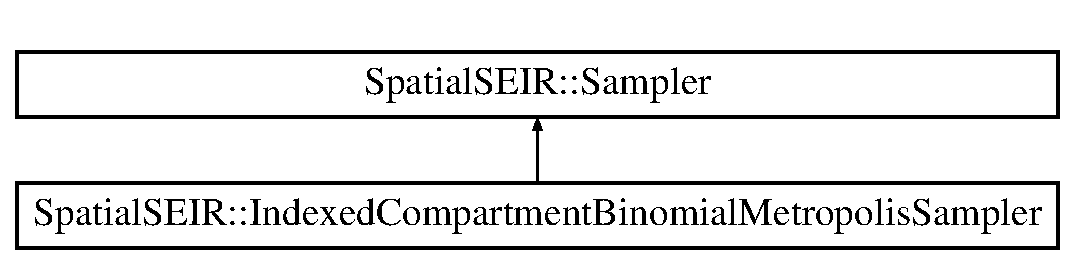
\includegraphics[height=2.000000cm]{classSpatialSEIR_1_1IndexedCompartmentBinomialMetropolisSampler}
\end{center}
\end{figure}
\subsection*{Public Member Functions}
\begin{DoxyCompactItemize}
\item 
\hyperlink{classSpatialSEIR_1_1IndexedCompartmentBinomialMetropolisSampler_ae6a8ff175ccc0a96d935b40dae644f76}{Indexed\-Compartment\-Binomial\-Metropolis\-Sampler} (\hyperlink{classSpatialSEIR_1_1ModelContext}{Model\-Context} $\ast$\hyperlink{classSpatialSEIR_1_1IndexedCompartmentBinomialMetropolisSampler_afcc687d3efa75c24937e4bc809928268}{context}, \hyperlink{classSpatialSEIR_1_1CompartmentFullConditional}{Compartment\-Full\-Conditional} $\ast$\hyperlink{classSpatialSEIR_1_1IndexedCompartmentBinomialMetropolisSampler_ab0db99c76bbf5ffdc939771362a872f7}{compartment\-F\-C}, int $\ast$\hyperlink{classSpatialSEIR_1_1IndexedCompartmentBinomialMetropolisSampler_accf1b0fb600a417c513fea3a3d65ea5d}{compartment\-Data}, int $\ast$\hyperlink{classSpatialSEIR_1_1IndexedCompartmentBinomialMetropolisSampler_a915bf551d29852056a3638b00e9a9404}{compartment\-From}, int $\ast$\hyperlink{classSpatialSEIR_1_1IndexedCompartmentBinomialMetropolisSampler_a97302172c15506865073ef44548ce6b0}{compartment\-To}, double $\ast$\hyperlink{classSpatialSEIR_1_1IndexedCompartmentBinomialMetropolisSampler_a1c9a06458af46193bf5a1a55b7652d4d}{probability\-Vector}, int \hyperlink{classSpatialSEIR_1_1IndexedCompartmentBinomialMetropolisSampler_af27c6ad0b6dec9387e298751dea30504}{probability\-Vector\-Len})
\item 
void \hyperlink{classSpatialSEIR_1_1IndexedCompartmentBinomialMetropolisSampler_a3f172aba5d9389b2193200a811d12142}{draw\-Sample} ()
\item 
int \hyperlink{classSpatialSEIR_1_1IndexedCompartmentBinomialMetropolisSampler_a2ce0af7bb2a881f254dfbd97584704bd}{get\-Sampler\-Type} ()
\item 
void \hyperlink{classSpatialSEIR_1_1IndexedCompartmentBinomialMetropolisSampler_af764b1c587bf46ef2198250bea987ace}{gen\-Proposal} ()
\item 
\hyperlink{classSpatialSEIR_1_1IndexedCompartmentBinomialMetropolisSampler_a34c4b58ae9a7550ce48f54a8c4c3ca6d}{$\sim$\-Indexed\-Compartment\-Binomial\-Metropolis\-Sampler} ()
\end{DoxyCompactItemize}
\subsection*{Public Attributes}
\begin{DoxyCompactItemize}
\item 
\hyperlink{classSpatialSEIR_1_1ModelContext}{Model\-Context} $\ast$$\ast$ \hyperlink{classSpatialSEIR_1_1IndexedCompartmentBinomialMetropolisSampler_afcc687d3efa75c24937e4bc809928268}{context}
\item 
\hyperlink{classSpatialSEIR_1_1CompartmentFullConditional}{Compartment\-Full\-Conditional} $\ast$$\ast$ \hyperlink{classSpatialSEIR_1_1IndexedCompartmentBinomialMetropolisSampler_ab0db99c76bbf5ffdc939771362a872f7}{compartment\-F\-C}
\item 
int $\ast$$\ast$ \hyperlink{classSpatialSEIR_1_1IndexedCompartmentBinomialMetropolisSampler_a8035e5cc93a9d3a9d66eb94d54362c7d}{index\-Length}
\item 
int $\ast$$\ast$ \hyperlink{classSpatialSEIR_1_1IndexedCompartmentBinomialMetropolisSampler_abbef44bf2436c1dec71cb6d7c521b0fe}{index\-List}
\item 
int $\ast$$\ast$ \hyperlink{classSpatialSEIR_1_1IndexedCompartmentBinomialMetropolisSampler_accf1b0fb600a417c513fea3a3d65ea5d}{compartment\-Data}
\item 
int $\ast$$\ast$ \hyperlink{classSpatialSEIR_1_1IndexedCompartmentBinomialMetropolisSampler_a915bf551d29852056a3638b00e9a9404}{compartment\-From}
\item 
int $\ast$$\ast$ \hyperlink{classSpatialSEIR_1_1IndexedCompartmentBinomialMetropolisSampler_a97302172c15506865073ef44548ce6b0}{compartment\-To}
\item 
double $\ast$$\ast$ \hyperlink{classSpatialSEIR_1_1IndexedCompartmentBinomialMetropolisSampler_a1c9a06458af46193bf5a1a55b7652d4d}{probability\-Vector}
\item 
int $\ast$ \hyperlink{classSpatialSEIR_1_1IndexedCompartmentBinomialMetropolisSampler_af27c6ad0b6dec9387e298751dea30504}{probability\-Vector\-Len}
\end{DoxyCompactItemize}


\subsection{Detailed Description}
The \hyperlink{classSpatialSEIR_1_1IndexedCompartmentBinomialMetropolisSampler}{Indexed\-Compartment\-Binomial\-Metropolis\-Sampler} class is child of the \hyperlink{classSpatialSEIR_1_1Sampler}{Sampler} class which draws samples from the posterior distribution of the various transition compartments using a chain binomial proposal based on the parameters, and uses the \hyperlink{classSpatialSEIR_1_1ModelContext}{Model\-Context} index to update only a portion of the compartment each iteration. 

\subsection{Constructor \& Destructor Documentation}
\hypertarget{classSpatialSEIR_1_1IndexedCompartmentBinomialMetropolisSampler_ae6a8ff175ccc0a96d935b40dae644f76}{\index{Spatial\-S\-E\-I\-R\-::\-Indexed\-Compartment\-Binomial\-Metropolis\-Sampler@{Spatial\-S\-E\-I\-R\-::\-Indexed\-Compartment\-Binomial\-Metropolis\-Sampler}!Indexed\-Compartment\-Binomial\-Metropolis\-Sampler@{Indexed\-Compartment\-Binomial\-Metropolis\-Sampler}}
\index{Indexed\-Compartment\-Binomial\-Metropolis\-Sampler@{Indexed\-Compartment\-Binomial\-Metropolis\-Sampler}!SpatialSEIR::IndexedCompartmentBinomialMetropolisSampler@{Spatial\-S\-E\-I\-R\-::\-Indexed\-Compartment\-Binomial\-Metropolis\-Sampler}}
\subsubsection[{Indexed\-Compartment\-Binomial\-Metropolis\-Sampler}]{\setlength{\rightskip}{0pt plus 5cm}Spatial\-S\-E\-I\-R\-::\-Indexed\-Compartment\-Binomial\-Metropolis\-Sampler\-::\-Indexed\-Compartment\-Binomial\-Metropolis\-Sampler (
\begin{DoxyParamCaption}
\item[{{\bf Model\-Context} $\ast$}]{context, }
\item[{{\bf Compartment\-Full\-Conditional} $\ast$}]{compartment\-F\-C, }
\item[{int $\ast$}]{compartment\-Data, }
\item[{int $\ast$}]{compartment\-From, }
\item[{int $\ast$}]{compartment\-To, }
\item[{double $\ast$}]{probability\-Vector, }
\item[{int}]{probability\-Vector\-Len}
\end{DoxyParamCaption}
)}}\label{classSpatialSEIR_1_1IndexedCompartmentBinomialMetropolisSampler_ae6a8ff175ccc0a96d935b40dae644f76}
\hypertarget{classSpatialSEIR_1_1IndexedCompartmentBinomialMetropolisSampler_a34c4b58ae9a7550ce48f54a8c4c3ca6d}{\index{Spatial\-S\-E\-I\-R\-::\-Indexed\-Compartment\-Binomial\-Metropolis\-Sampler@{Spatial\-S\-E\-I\-R\-::\-Indexed\-Compartment\-Binomial\-Metropolis\-Sampler}!$\sim$\-Indexed\-Compartment\-Binomial\-Metropolis\-Sampler@{$\sim$\-Indexed\-Compartment\-Binomial\-Metropolis\-Sampler}}
\index{$\sim$\-Indexed\-Compartment\-Binomial\-Metropolis\-Sampler@{$\sim$\-Indexed\-Compartment\-Binomial\-Metropolis\-Sampler}!SpatialSEIR::IndexedCompartmentBinomialMetropolisSampler@{Spatial\-S\-E\-I\-R\-::\-Indexed\-Compartment\-Binomial\-Metropolis\-Sampler}}
\subsubsection[{$\sim$\-Indexed\-Compartment\-Binomial\-Metropolis\-Sampler}]{\setlength{\rightskip}{0pt plus 5cm}Spatial\-S\-E\-I\-R\-::\-Indexed\-Compartment\-Binomial\-Metropolis\-Sampler\-::$\sim$\-Indexed\-Compartment\-Binomial\-Metropolis\-Sampler (
\begin{DoxyParamCaption}
{}
\end{DoxyParamCaption}
)}}\label{classSpatialSEIR_1_1IndexedCompartmentBinomialMetropolisSampler_a34c4b58ae9a7550ce48f54a8c4c3ca6d}


\subsection{Member Function Documentation}
\hypertarget{classSpatialSEIR_1_1IndexedCompartmentBinomialMetropolisSampler_a3f172aba5d9389b2193200a811d12142}{\index{Spatial\-S\-E\-I\-R\-::\-Indexed\-Compartment\-Binomial\-Metropolis\-Sampler@{Spatial\-S\-E\-I\-R\-::\-Indexed\-Compartment\-Binomial\-Metropolis\-Sampler}!draw\-Sample@{draw\-Sample}}
\index{draw\-Sample@{draw\-Sample}!SpatialSEIR::IndexedCompartmentBinomialMetropolisSampler@{Spatial\-S\-E\-I\-R\-::\-Indexed\-Compartment\-Binomial\-Metropolis\-Sampler}}
\subsubsection[{draw\-Sample}]{\setlength{\rightskip}{0pt plus 5cm}void Spatial\-S\-E\-I\-R\-::\-Indexed\-Compartment\-Binomial\-Metropolis\-Sampler\-::draw\-Sample (
\begin{DoxyParamCaption}
{}
\end{DoxyParamCaption}
)\hspace{0.3cm}{\ttfamily [virtual]}}}\label{classSpatialSEIR_1_1IndexedCompartmentBinomialMetropolisSampler_a3f172aba5d9389b2193200a811d12142}


Implements \hyperlink{classSpatialSEIR_1_1Sampler_aa07a42b26cb62249c20c58e855a08657}{Spatial\-S\-E\-I\-R\-::\-Sampler}.

\hypertarget{classSpatialSEIR_1_1IndexedCompartmentBinomialMetropolisSampler_af764b1c587bf46ef2198250bea987ace}{\index{Spatial\-S\-E\-I\-R\-::\-Indexed\-Compartment\-Binomial\-Metropolis\-Sampler@{Spatial\-S\-E\-I\-R\-::\-Indexed\-Compartment\-Binomial\-Metropolis\-Sampler}!gen\-Proposal@{gen\-Proposal}}
\index{gen\-Proposal@{gen\-Proposal}!SpatialSEIR::IndexedCompartmentBinomialMetropolisSampler@{Spatial\-S\-E\-I\-R\-::\-Indexed\-Compartment\-Binomial\-Metropolis\-Sampler}}
\subsubsection[{gen\-Proposal}]{\setlength{\rightskip}{0pt plus 5cm}void Spatial\-S\-E\-I\-R\-::\-Indexed\-Compartment\-Binomial\-Metropolis\-Sampler\-::gen\-Proposal (
\begin{DoxyParamCaption}
{}
\end{DoxyParamCaption}
)}}\label{classSpatialSEIR_1_1IndexedCompartmentBinomialMetropolisSampler_af764b1c587bf46ef2198250bea987ace}
\hypertarget{classSpatialSEIR_1_1IndexedCompartmentBinomialMetropolisSampler_a2ce0af7bb2a881f254dfbd97584704bd}{\index{Spatial\-S\-E\-I\-R\-::\-Indexed\-Compartment\-Binomial\-Metropolis\-Sampler@{Spatial\-S\-E\-I\-R\-::\-Indexed\-Compartment\-Binomial\-Metropolis\-Sampler}!get\-Sampler\-Type@{get\-Sampler\-Type}}
\index{get\-Sampler\-Type@{get\-Sampler\-Type}!SpatialSEIR::IndexedCompartmentBinomialMetropolisSampler@{Spatial\-S\-E\-I\-R\-::\-Indexed\-Compartment\-Binomial\-Metropolis\-Sampler}}
\subsubsection[{get\-Sampler\-Type}]{\setlength{\rightskip}{0pt plus 5cm}int Spatial\-S\-E\-I\-R\-::\-Indexed\-Compartment\-Binomial\-Metropolis\-Sampler\-::get\-Sampler\-Type (
\begin{DoxyParamCaption}
{}
\end{DoxyParamCaption}
)\hspace{0.3cm}{\ttfamily [virtual]}}}\label{classSpatialSEIR_1_1IndexedCompartmentBinomialMetropolisSampler_a2ce0af7bb2a881f254dfbd97584704bd}


Implements \hyperlink{classSpatialSEIR_1_1Sampler_aaa79310ad809e6aeb25479849f322dda}{Spatial\-S\-E\-I\-R\-::\-Sampler}.



\subsection{Member Data Documentation}
\hypertarget{classSpatialSEIR_1_1IndexedCompartmentBinomialMetropolisSampler_accf1b0fb600a417c513fea3a3d65ea5d}{\index{Spatial\-S\-E\-I\-R\-::\-Indexed\-Compartment\-Binomial\-Metropolis\-Sampler@{Spatial\-S\-E\-I\-R\-::\-Indexed\-Compartment\-Binomial\-Metropolis\-Sampler}!compartment\-Data@{compartment\-Data}}
\index{compartment\-Data@{compartment\-Data}!SpatialSEIR::IndexedCompartmentBinomialMetropolisSampler@{Spatial\-S\-E\-I\-R\-::\-Indexed\-Compartment\-Binomial\-Metropolis\-Sampler}}
\subsubsection[{compartment\-Data}]{\setlength{\rightskip}{0pt plus 5cm}int$\ast$$\ast$ Spatial\-S\-E\-I\-R\-::\-Indexed\-Compartment\-Binomial\-Metropolis\-Sampler\-::compartment\-Data}}\label{classSpatialSEIR_1_1IndexedCompartmentBinomialMetropolisSampler_accf1b0fb600a417c513fea3a3d65ea5d}
\hypertarget{classSpatialSEIR_1_1IndexedCompartmentBinomialMetropolisSampler_ab0db99c76bbf5ffdc939771362a872f7}{\index{Spatial\-S\-E\-I\-R\-::\-Indexed\-Compartment\-Binomial\-Metropolis\-Sampler@{Spatial\-S\-E\-I\-R\-::\-Indexed\-Compartment\-Binomial\-Metropolis\-Sampler}!compartment\-F\-C@{compartment\-F\-C}}
\index{compartment\-F\-C@{compartment\-F\-C}!SpatialSEIR::IndexedCompartmentBinomialMetropolisSampler@{Spatial\-S\-E\-I\-R\-::\-Indexed\-Compartment\-Binomial\-Metropolis\-Sampler}}
\subsubsection[{compartment\-F\-C}]{\setlength{\rightskip}{0pt plus 5cm}{\bf Compartment\-Full\-Conditional}$\ast$$\ast$ Spatial\-S\-E\-I\-R\-::\-Indexed\-Compartment\-Binomial\-Metropolis\-Sampler\-::compartment\-F\-C}}\label{classSpatialSEIR_1_1IndexedCompartmentBinomialMetropolisSampler_ab0db99c76bbf5ffdc939771362a872f7}
\hypertarget{classSpatialSEIR_1_1IndexedCompartmentBinomialMetropolisSampler_a915bf551d29852056a3638b00e9a9404}{\index{Spatial\-S\-E\-I\-R\-::\-Indexed\-Compartment\-Binomial\-Metropolis\-Sampler@{Spatial\-S\-E\-I\-R\-::\-Indexed\-Compartment\-Binomial\-Metropolis\-Sampler}!compartment\-From@{compartment\-From}}
\index{compartment\-From@{compartment\-From}!SpatialSEIR::IndexedCompartmentBinomialMetropolisSampler@{Spatial\-S\-E\-I\-R\-::\-Indexed\-Compartment\-Binomial\-Metropolis\-Sampler}}
\subsubsection[{compartment\-From}]{\setlength{\rightskip}{0pt plus 5cm}int$\ast$$\ast$ Spatial\-S\-E\-I\-R\-::\-Indexed\-Compartment\-Binomial\-Metropolis\-Sampler\-::compartment\-From}}\label{classSpatialSEIR_1_1IndexedCompartmentBinomialMetropolisSampler_a915bf551d29852056a3638b00e9a9404}
\hypertarget{classSpatialSEIR_1_1IndexedCompartmentBinomialMetropolisSampler_a97302172c15506865073ef44548ce6b0}{\index{Spatial\-S\-E\-I\-R\-::\-Indexed\-Compartment\-Binomial\-Metropolis\-Sampler@{Spatial\-S\-E\-I\-R\-::\-Indexed\-Compartment\-Binomial\-Metropolis\-Sampler}!compartment\-To@{compartment\-To}}
\index{compartment\-To@{compartment\-To}!SpatialSEIR::IndexedCompartmentBinomialMetropolisSampler@{Spatial\-S\-E\-I\-R\-::\-Indexed\-Compartment\-Binomial\-Metropolis\-Sampler}}
\subsubsection[{compartment\-To}]{\setlength{\rightskip}{0pt plus 5cm}int$\ast$$\ast$ Spatial\-S\-E\-I\-R\-::\-Indexed\-Compartment\-Binomial\-Metropolis\-Sampler\-::compartment\-To}}\label{classSpatialSEIR_1_1IndexedCompartmentBinomialMetropolisSampler_a97302172c15506865073ef44548ce6b0}
\hypertarget{classSpatialSEIR_1_1IndexedCompartmentBinomialMetropolisSampler_afcc687d3efa75c24937e4bc809928268}{\index{Spatial\-S\-E\-I\-R\-::\-Indexed\-Compartment\-Binomial\-Metropolis\-Sampler@{Spatial\-S\-E\-I\-R\-::\-Indexed\-Compartment\-Binomial\-Metropolis\-Sampler}!context@{context}}
\index{context@{context}!SpatialSEIR::IndexedCompartmentBinomialMetropolisSampler@{Spatial\-S\-E\-I\-R\-::\-Indexed\-Compartment\-Binomial\-Metropolis\-Sampler}}
\subsubsection[{context}]{\setlength{\rightskip}{0pt plus 5cm}{\bf Model\-Context}$\ast$$\ast$ Spatial\-S\-E\-I\-R\-::\-Indexed\-Compartment\-Binomial\-Metropolis\-Sampler\-::context}}\label{classSpatialSEIR_1_1IndexedCompartmentBinomialMetropolisSampler_afcc687d3efa75c24937e4bc809928268}
\hypertarget{classSpatialSEIR_1_1IndexedCompartmentBinomialMetropolisSampler_a8035e5cc93a9d3a9d66eb94d54362c7d}{\index{Spatial\-S\-E\-I\-R\-::\-Indexed\-Compartment\-Binomial\-Metropolis\-Sampler@{Spatial\-S\-E\-I\-R\-::\-Indexed\-Compartment\-Binomial\-Metropolis\-Sampler}!index\-Length@{index\-Length}}
\index{index\-Length@{index\-Length}!SpatialSEIR::IndexedCompartmentBinomialMetropolisSampler@{Spatial\-S\-E\-I\-R\-::\-Indexed\-Compartment\-Binomial\-Metropolis\-Sampler}}
\subsubsection[{index\-Length}]{\setlength{\rightskip}{0pt plus 5cm}int$\ast$$\ast$ Spatial\-S\-E\-I\-R\-::\-Indexed\-Compartment\-Binomial\-Metropolis\-Sampler\-::index\-Length}}\label{classSpatialSEIR_1_1IndexedCompartmentBinomialMetropolisSampler_a8035e5cc93a9d3a9d66eb94d54362c7d}
\hypertarget{classSpatialSEIR_1_1IndexedCompartmentBinomialMetropolisSampler_abbef44bf2436c1dec71cb6d7c521b0fe}{\index{Spatial\-S\-E\-I\-R\-::\-Indexed\-Compartment\-Binomial\-Metropolis\-Sampler@{Spatial\-S\-E\-I\-R\-::\-Indexed\-Compartment\-Binomial\-Metropolis\-Sampler}!index\-List@{index\-List}}
\index{index\-List@{index\-List}!SpatialSEIR::IndexedCompartmentBinomialMetropolisSampler@{Spatial\-S\-E\-I\-R\-::\-Indexed\-Compartment\-Binomial\-Metropolis\-Sampler}}
\subsubsection[{index\-List}]{\setlength{\rightskip}{0pt plus 5cm}int$\ast$$\ast$ Spatial\-S\-E\-I\-R\-::\-Indexed\-Compartment\-Binomial\-Metropolis\-Sampler\-::index\-List}}\label{classSpatialSEIR_1_1IndexedCompartmentBinomialMetropolisSampler_abbef44bf2436c1dec71cb6d7c521b0fe}
\hypertarget{classSpatialSEIR_1_1IndexedCompartmentBinomialMetropolisSampler_a1c9a06458af46193bf5a1a55b7652d4d}{\index{Spatial\-S\-E\-I\-R\-::\-Indexed\-Compartment\-Binomial\-Metropolis\-Sampler@{Spatial\-S\-E\-I\-R\-::\-Indexed\-Compartment\-Binomial\-Metropolis\-Sampler}!probability\-Vector@{probability\-Vector}}
\index{probability\-Vector@{probability\-Vector}!SpatialSEIR::IndexedCompartmentBinomialMetropolisSampler@{Spatial\-S\-E\-I\-R\-::\-Indexed\-Compartment\-Binomial\-Metropolis\-Sampler}}
\subsubsection[{probability\-Vector}]{\setlength{\rightskip}{0pt plus 5cm}double$\ast$$\ast$ Spatial\-S\-E\-I\-R\-::\-Indexed\-Compartment\-Binomial\-Metropolis\-Sampler\-::probability\-Vector}}\label{classSpatialSEIR_1_1IndexedCompartmentBinomialMetropolisSampler_a1c9a06458af46193bf5a1a55b7652d4d}
\hypertarget{classSpatialSEIR_1_1IndexedCompartmentBinomialMetropolisSampler_af27c6ad0b6dec9387e298751dea30504}{\index{Spatial\-S\-E\-I\-R\-::\-Indexed\-Compartment\-Binomial\-Metropolis\-Sampler@{Spatial\-S\-E\-I\-R\-::\-Indexed\-Compartment\-Binomial\-Metropolis\-Sampler}!probability\-Vector\-Len@{probability\-Vector\-Len}}
\index{probability\-Vector\-Len@{probability\-Vector\-Len}!SpatialSEIR::IndexedCompartmentBinomialMetropolisSampler@{Spatial\-S\-E\-I\-R\-::\-Indexed\-Compartment\-Binomial\-Metropolis\-Sampler}}
\subsubsection[{probability\-Vector\-Len}]{\setlength{\rightskip}{0pt plus 5cm}int$\ast$ Spatial\-S\-E\-I\-R\-::\-Indexed\-Compartment\-Binomial\-Metropolis\-Sampler\-::probability\-Vector\-Len}}\label{classSpatialSEIR_1_1IndexedCompartmentBinomialMetropolisSampler_af27c6ad0b6dec9387e298751dea30504}


The documentation for this class was generated from the following file\-:\begin{DoxyCompactItemize}
\item 
lib\-Spatial\-S\-E\-I\-R/include/\hyperlink{LSS__Samplers_8hpp}{L\-S\-S\-\_\-\-Samplers.\-hpp}\end{DoxyCompactItemize}

\hypertarget{classSpatialSEIR_1_1IndexedCompartmentMetropolisSampler}{\section{Spatial\-S\-E\-I\-R\-:\-:Indexed\-Compartment\-Metropolis\-Sampler Class Reference}
\label{classSpatialSEIR_1_1IndexedCompartmentMetropolisSampler}\index{Spatial\-S\-E\-I\-R\-::\-Indexed\-Compartment\-Metropolis\-Sampler@{Spatial\-S\-E\-I\-R\-::\-Indexed\-Compartment\-Metropolis\-Sampler}}
}


{\ttfamily \#include $<$L\-S\-S\-\_\-\-Samplers.\-hpp$>$}

Inheritance diagram for Spatial\-S\-E\-I\-R\-:\-:Indexed\-Compartment\-Metropolis\-Sampler\-:\begin{figure}[H]
\begin{center}
\leavevmode
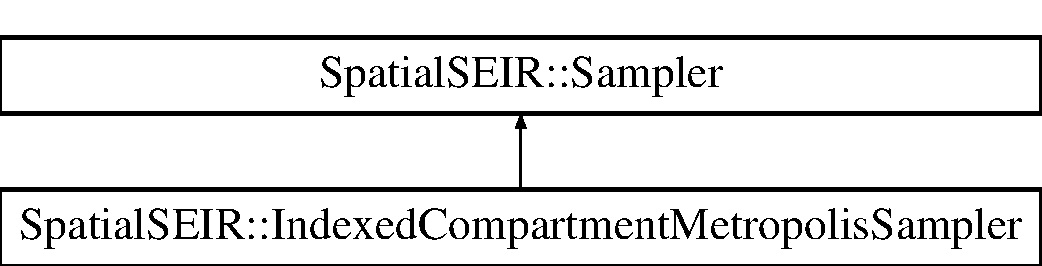
\includegraphics[height=2.000000cm]{classSpatialSEIR_1_1IndexedCompartmentMetropolisSampler}
\end{center}
\end{figure}
\subsection*{Public Member Functions}
\begin{DoxyCompactItemize}
\item 
\hyperlink{classSpatialSEIR_1_1IndexedCompartmentMetropolisSampler_ab854404a8d8d53fc77be7a7a90937e43}{Indexed\-Compartment\-Metropolis\-Sampler} (\hyperlink{classSpatialSEIR_1_1ModelContext}{Model\-Context} $\ast$\hyperlink{classSpatialSEIR_1_1IndexedCompartmentMetropolisSampler_a83b05275c5b6e2da4d336eb09d7bb2b5}{context}, \hyperlink{classSpatialSEIR_1_1CompartmentFullConditional}{Compartment\-Full\-Conditional} $\ast$\hyperlink{classSpatialSEIR_1_1IndexedCompartmentMetropolisSampler_a67e3744835088d5612fbc3caf85dbac2}{compartment\-F\-C}, int $\ast$\hyperlink{classSpatialSEIR_1_1IndexedCompartmentMetropolisSampler_ad82e142ca51ec5b9099d4fce0ceed7c3}{compartment\-Data})
\item 
void \hyperlink{classSpatialSEIR_1_1IndexedCompartmentMetropolisSampler_a98bcf6dc5e426a45ef11bf04c1e178dd}{draw\-Sample} ()
\item 
int \hyperlink{classSpatialSEIR_1_1IndexedCompartmentMetropolisSampler_a87fe511f9a9fd517c4bafad59c296986}{get\-Sampler\-Type} ()
\item 
\hyperlink{classSpatialSEIR_1_1IndexedCompartmentMetropolisSampler_a9196ae6955cec850a05b1d6f7784e941}{$\sim$\-Indexed\-Compartment\-Metropolis\-Sampler} ()
\end{DoxyCompactItemize}
\subsection*{Public Attributes}
\begin{DoxyCompactItemize}
\item 
\hyperlink{classSpatialSEIR_1_1ModelContext}{Model\-Context} $\ast$$\ast$ \hyperlink{classSpatialSEIR_1_1IndexedCompartmentMetropolisSampler_a83b05275c5b6e2da4d336eb09d7bb2b5}{context}
\item 
\hyperlink{classSpatialSEIR_1_1CompartmentFullConditional}{Compartment\-Full\-Conditional} $\ast$$\ast$ \hyperlink{classSpatialSEIR_1_1IndexedCompartmentMetropolisSampler_a67e3744835088d5612fbc3caf85dbac2}{compartment\-F\-C}
\item 
int $\ast$$\ast$ \hyperlink{classSpatialSEIR_1_1IndexedCompartmentMetropolisSampler_adb184082c1e6f3a4065edee600f69c1b}{index\-Length}
\item 
int $\ast$$\ast$ \hyperlink{classSpatialSEIR_1_1IndexedCompartmentMetropolisSampler_ad82e142ca51ec5b9099d4fce0ceed7c3}{compartment\-Data}
\item 
int $\ast$$\ast$ \hyperlink{classSpatialSEIR_1_1IndexedCompartmentMetropolisSampler_a69b2f84b4fe8bbb44831a106b3d55bfe}{index\-List}
\end{DoxyCompactItemize}


\subsection{Detailed Description}
The \hyperlink{classSpatialSEIR_1_1IndexedCompartmentMetropolisSampler}{Indexed\-Compartment\-Metropolis\-Sampler} class is child of the \hyperlink{classSpatialSEIR_1_1Sampler}{Sampler} class which draws samples from the posterior distribution of the various transition compartments using a partial Metropolis proposal, with proposal indices determined by the \hyperlink{classSpatialSEIR_1_1ModelContext}{Model\-Context} to which it belongs. This sampler is designed to reduce autocorrelation by letting all compartments move together using the same indices. 

\subsection{Constructor \& Destructor Documentation}
\hypertarget{classSpatialSEIR_1_1IndexedCompartmentMetropolisSampler_ab854404a8d8d53fc77be7a7a90937e43}{\index{Spatial\-S\-E\-I\-R\-::\-Indexed\-Compartment\-Metropolis\-Sampler@{Spatial\-S\-E\-I\-R\-::\-Indexed\-Compartment\-Metropolis\-Sampler}!Indexed\-Compartment\-Metropolis\-Sampler@{Indexed\-Compartment\-Metropolis\-Sampler}}
\index{Indexed\-Compartment\-Metropolis\-Sampler@{Indexed\-Compartment\-Metropolis\-Sampler}!SpatialSEIR::IndexedCompartmentMetropolisSampler@{Spatial\-S\-E\-I\-R\-::\-Indexed\-Compartment\-Metropolis\-Sampler}}
\subsubsection[{Indexed\-Compartment\-Metropolis\-Sampler}]{\setlength{\rightskip}{0pt plus 5cm}Spatial\-S\-E\-I\-R\-::\-Indexed\-Compartment\-Metropolis\-Sampler\-::\-Indexed\-Compartment\-Metropolis\-Sampler (
\begin{DoxyParamCaption}
\item[{{\bf Model\-Context} $\ast$}]{context, }
\item[{{\bf Compartment\-Full\-Conditional} $\ast$}]{compartment\-F\-C, }
\item[{int $\ast$}]{compartment\-Data}
\end{DoxyParamCaption}
)}}\label{classSpatialSEIR_1_1IndexedCompartmentMetropolisSampler_ab854404a8d8d53fc77be7a7a90937e43}
\hypertarget{classSpatialSEIR_1_1IndexedCompartmentMetropolisSampler_a9196ae6955cec850a05b1d6f7784e941}{\index{Spatial\-S\-E\-I\-R\-::\-Indexed\-Compartment\-Metropolis\-Sampler@{Spatial\-S\-E\-I\-R\-::\-Indexed\-Compartment\-Metropolis\-Sampler}!$\sim$\-Indexed\-Compartment\-Metropolis\-Sampler@{$\sim$\-Indexed\-Compartment\-Metropolis\-Sampler}}
\index{$\sim$\-Indexed\-Compartment\-Metropolis\-Sampler@{$\sim$\-Indexed\-Compartment\-Metropolis\-Sampler}!SpatialSEIR::IndexedCompartmentMetropolisSampler@{Spatial\-S\-E\-I\-R\-::\-Indexed\-Compartment\-Metropolis\-Sampler}}
\subsubsection[{$\sim$\-Indexed\-Compartment\-Metropolis\-Sampler}]{\setlength{\rightskip}{0pt plus 5cm}Spatial\-S\-E\-I\-R\-::\-Indexed\-Compartment\-Metropolis\-Sampler\-::$\sim$\-Indexed\-Compartment\-Metropolis\-Sampler (
\begin{DoxyParamCaption}
{}
\end{DoxyParamCaption}
)}}\label{classSpatialSEIR_1_1IndexedCompartmentMetropolisSampler_a9196ae6955cec850a05b1d6f7784e941}


\subsection{Member Function Documentation}
\hypertarget{classSpatialSEIR_1_1IndexedCompartmentMetropolisSampler_a98bcf6dc5e426a45ef11bf04c1e178dd}{\index{Spatial\-S\-E\-I\-R\-::\-Indexed\-Compartment\-Metropolis\-Sampler@{Spatial\-S\-E\-I\-R\-::\-Indexed\-Compartment\-Metropolis\-Sampler}!draw\-Sample@{draw\-Sample}}
\index{draw\-Sample@{draw\-Sample}!SpatialSEIR::IndexedCompartmentMetropolisSampler@{Spatial\-S\-E\-I\-R\-::\-Indexed\-Compartment\-Metropolis\-Sampler}}
\subsubsection[{draw\-Sample}]{\setlength{\rightskip}{0pt plus 5cm}void Spatial\-S\-E\-I\-R\-::\-Indexed\-Compartment\-Metropolis\-Sampler\-::draw\-Sample (
\begin{DoxyParamCaption}
{}
\end{DoxyParamCaption}
)\hspace{0.3cm}{\ttfamily [virtual]}}}\label{classSpatialSEIR_1_1IndexedCompartmentMetropolisSampler_a98bcf6dc5e426a45ef11bf04c1e178dd}


Implements \hyperlink{classSpatialSEIR_1_1Sampler_aa07a42b26cb62249c20c58e855a08657}{Spatial\-S\-E\-I\-R\-::\-Sampler}.

\hypertarget{classSpatialSEIR_1_1IndexedCompartmentMetropolisSampler_a87fe511f9a9fd517c4bafad59c296986}{\index{Spatial\-S\-E\-I\-R\-::\-Indexed\-Compartment\-Metropolis\-Sampler@{Spatial\-S\-E\-I\-R\-::\-Indexed\-Compartment\-Metropolis\-Sampler}!get\-Sampler\-Type@{get\-Sampler\-Type}}
\index{get\-Sampler\-Type@{get\-Sampler\-Type}!SpatialSEIR::IndexedCompartmentMetropolisSampler@{Spatial\-S\-E\-I\-R\-::\-Indexed\-Compartment\-Metropolis\-Sampler}}
\subsubsection[{get\-Sampler\-Type}]{\setlength{\rightskip}{0pt plus 5cm}int Spatial\-S\-E\-I\-R\-::\-Indexed\-Compartment\-Metropolis\-Sampler\-::get\-Sampler\-Type (
\begin{DoxyParamCaption}
{}
\end{DoxyParamCaption}
)\hspace{0.3cm}{\ttfamily [virtual]}}}\label{classSpatialSEIR_1_1IndexedCompartmentMetropolisSampler_a87fe511f9a9fd517c4bafad59c296986}


Implements \hyperlink{classSpatialSEIR_1_1Sampler_aaa79310ad809e6aeb25479849f322dda}{Spatial\-S\-E\-I\-R\-::\-Sampler}.



\subsection{Member Data Documentation}
\hypertarget{classSpatialSEIR_1_1IndexedCompartmentMetropolisSampler_ad82e142ca51ec5b9099d4fce0ceed7c3}{\index{Spatial\-S\-E\-I\-R\-::\-Indexed\-Compartment\-Metropolis\-Sampler@{Spatial\-S\-E\-I\-R\-::\-Indexed\-Compartment\-Metropolis\-Sampler}!compartment\-Data@{compartment\-Data}}
\index{compartment\-Data@{compartment\-Data}!SpatialSEIR::IndexedCompartmentMetropolisSampler@{Spatial\-S\-E\-I\-R\-::\-Indexed\-Compartment\-Metropolis\-Sampler}}
\subsubsection[{compartment\-Data}]{\setlength{\rightskip}{0pt plus 5cm}int$\ast$$\ast$ Spatial\-S\-E\-I\-R\-::\-Indexed\-Compartment\-Metropolis\-Sampler\-::compartment\-Data}}\label{classSpatialSEIR_1_1IndexedCompartmentMetropolisSampler_ad82e142ca51ec5b9099d4fce0ceed7c3}
\hypertarget{classSpatialSEIR_1_1IndexedCompartmentMetropolisSampler_a67e3744835088d5612fbc3caf85dbac2}{\index{Spatial\-S\-E\-I\-R\-::\-Indexed\-Compartment\-Metropolis\-Sampler@{Spatial\-S\-E\-I\-R\-::\-Indexed\-Compartment\-Metropolis\-Sampler}!compartment\-F\-C@{compartment\-F\-C}}
\index{compartment\-F\-C@{compartment\-F\-C}!SpatialSEIR::IndexedCompartmentMetropolisSampler@{Spatial\-S\-E\-I\-R\-::\-Indexed\-Compartment\-Metropolis\-Sampler}}
\subsubsection[{compartment\-F\-C}]{\setlength{\rightskip}{0pt plus 5cm}{\bf Compartment\-Full\-Conditional}$\ast$$\ast$ Spatial\-S\-E\-I\-R\-::\-Indexed\-Compartment\-Metropolis\-Sampler\-::compartment\-F\-C}}\label{classSpatialSEIR_1_1IndexedCompartmentMetropolisSampler_a67e3744835088d5612fbc3caf85dbac2}
\hypertarget{classSpatialSEIR_1_1IndexedCompartmentMetropolisSampler_a83b05275c5b6e2da4d336eb09d7bb2b5}{\index{Spatial\-S\-E\-I\-R\-::\-Indexed\-Compartment\-Metropolis\-Sampler@{Spatial\-S\-E\-I\-R\-::\-Indexed\-Compartment\-Metropolis\-Sampler}!context@{context}}
\index{context@{context}!SpatialSEIR::IndexedCompartmentMetropolisSampler@{Spatial\-S\-E\-I\-R\-::\-Indexed\-Compartment\-Metropolis\-Sampler}}
\subsubsection[{context}]{\setlength{\rightskip}{0pt plus 5cm}{\bf Model\-Context}$\ast$$\ast$ Spatial\-S\-E\-I\-R\-::\-Indexed\-Compartment\-Metropolis\-Sampler\-::context}}\label{classSpatialSEIR_1_1IndexedCompartmentMetropolisSampler_a83b05275c5b6e2da4d336eb09d7bb2b5}
\hypertarget{classSpatialSEIR_1_1IndexedCompartmentMetropolisSampler_adb184082c1e6f3a4065edee600f69c1b}{\index{Spatial\-S\-E\-I\-R\-::\-Indexed\-Compartment\-Metropolis\-Sampler@{Spatial\-S\-E\-I\-R\-::\-Indexed\-Compartment\-Metropolis\-Sampler}!index\-Length@{index\-Length}}
\index{index\-Length@{index\-Length}!SpatialSEIR::IndexedCompartmentMetropolisSampler@{Spatial\-S\-E\-I\-R\-::\-Indexed\-Compartment\-Metropolis\-Sampler}}
\subsubsection[{index\-Length}]{\setlength{\rightskip}{0pt plus 5cm}int$\ast$$\ast$ Spatial\-S\-E\-I\-R\-::\-Indexed\-Compartment\-Metropolis\-Sampler\-::index\-Length}}\label{classSpatialSEIR_1_1IndexedCompartmentMetropolisSampler_adb184082c1e6f3a4065edee600f69c1b}
\hypertarget{classSpatialSEIR_1_1IndexedCompartmentMetropolisSampler_a69b2f84b4fe8bbb44831a106b3d55bfe}{\index{Spatial\-S\-E\-I\-R\-::\-Indexed\-Compartment\-Metropolis\-Sampler@{Spatial\-S\-E\-I\-R\-::\-Indexed\-Compartment\-Metropolis\-Sampler}!index\-List@{index\-List}}
\index{index\-List@{index\-List}!SpatialSEIR::IndexedCompartmentMetropolisSampler@{Spatial\-S\-E\-I\-R\-::\-Indexed\-Compartment\-Metropolis\-Sampler}}
\subsubsection[{index\-List}]{\setlength{\rightskip}{0pt plus 5cm}int$\ast$$\ast$ Spatial\-S\-E\-I\-R\-::\-Indexed\-Compartment\-Metropolis\-Sampler\-::index\-List}}\label{classSpatialSEIR_1_1IndexedCompartmentMetropolisSampler_a69b2f84b4fe8bbb44831a106b3d55bfe}


The documentation for this class was generated from the following file\-:\begin{DoxyCompactItemize}
\item 
lib\-Spatial\-S\-E\-I\-R/include/\hyperlink{LSS__Samplers_8hpp}{L\-S\-S\-\_\-\-Samplers.\-hpp}\end{DoxyCompactItemize}

\hypertarget{classSpatialSEIR_1_1IndexedCompartmentSliceSampler}{\section{Spatial\-S\-E\-I\-R\-:\-:Indexed\-Compartment\-Slice\-Sampler Class Reference}
\label{classSpatialSEIR_1_1IndexedCompartmentSliceSampler}\index{Spatial\-S\-E\-I\-R\-::\-Indexed\-Compartment\-Slice\-Sampler@{Spatial\-S\-E\-I\-R\-::\-Indexed\-Compartment\-Slice\-Sampler}}
}


{\ttfamily \#include $<$L\-S\-S\-\_\-\-Samplers.\-hpp$>$}

Inheritance diagram for Spatial\-S\-E\-I\-R\-:\-:Indexed\-Compartment\-Slice\-Sampler\-:\begin{figure}[H]
\begin{center}
\leavevmode
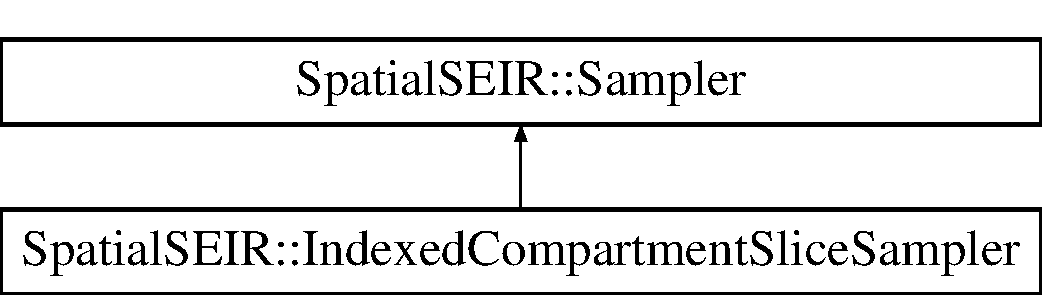
\includegraphics[height=2.000000cm]{classSpatialSEIR_1_1IndexedCompartmentSliceSampler}
\end{center}
\end{figure}
\subsection*{Public Member Functions}
\begin{DoxyCompactItemize}
\item 
\hyperlink{classSpatialSEIR_1_1IndexedCompartmentSliceSampler_afc64640b7a48fa0d4785d178cbfb0b93}{Indexed\-Compartment\-Slice\-Sampler} (\hyperlink{classSpatialSEIR_1_1ModelContext}{Model\-Context} $\ast$\hyperlink{classSpatialSEIR_1_1IndexedCompartmentSliceSampler_a387edb6d90edf9b39452985db5accfd4}{context}, \hyperlink{classSpatialSEIR_1_1CompartmentFullConditional}{Compartment\-Full\-Conditional} $\ast$\hyperlink{classSpatialSEIR_1_1IndexedCompartmentSliceSampler_a7fc85c9a378b1d9fc0e23f98500c92ba}{compartment\-F\-C}, int $\ast$\hyperlink{classSpatialSEIR_1_1IndexedCompartmentSliceSampler_ad5b34688ef3b6a8ee52fdcde13308be5}{compartment\-Data})
\item 
void \hyperlink{classSpatialSEIR_1_1IndexedCompartmentSliceSampler_aba6f0bd34d4fc684ac844767a09dab95}{draw\-Sample} ()
\item 
int \hyperlink{classSpatialSEIR_1_1IndexedCompartmentSliceSampler_aeeeeb33f86bf684e6e44914c784847e6}{get\-Sampler\-Type} ()
\item 
\hyperlink{classSpatialSEIR_1_1IndexedCompartmentSliceSampler_a5b26b72e037ed9956acd2bf15ed87ac7}{$\sim$\-Indexed\-Compartment\-Slice\-Sampler} ()
\end{DoxyCompactItemize}
\subsection*{Public Attributes}
\begin{DoxyCompactItemize}
\item 
\hyperlink{classSpatialSEIR_1_1ModelContext}{Model\-Context} $\ast$$\ast$ \hyperlink{classSpatialSEIR_1_1IndexedCompartmentSliceSampler_a387edb6d90edf9b39452985db5accfd4}{context}
\item 
\hyperlink{classSpatialSEIR_1_1CompartmentFullConditional}{Compartment\-Full\-Conditional} $\ast$$\ast$ \hyperlink{classSpatialSEIR_1_1IndexedCompartmentSliceSampler_a7fc85c9a378b1d9fc0e23f98500c92ba}{compartment\-F\-C}
\item 
int $\ast$$\ast$ \hyperlink{classSpatialSEIR_1_1IndexedCompartmentSliceSampler_ada391aecf581b46873e89a3c6c600859}{index\-Length}
\item 
int $\ast$$\ast$ \hyperlink{classSpatialSEIR_1_1IndexedCompartmentSliceSampler_ad5b34688ef3b6a8ee52fdcde13308be5}{compartment\-Data}
\item 
int $\ast$$\ast$ \hyperlink{classSpatialSEIR_1_1IndexedCompartmentSliceSampler_ad52c949b38fc58f6f734aeb589655c20}{index\-List}
\end{DoxyCompactItemize}


\subsection{Detailed Description}
The \hyperlink{classSpatialSEIR_1_1IndexedCompartmentSliceSampler}{Indexed\-Compartment\-Slice\-Sampler} class is child of the \hyperlink{classSpatialSEIR_1_1Sampler}{Sampler} class which draws samples from the posterior distribution of the various transition compartments using a partial slice sampling proposal, with proposal indices determined by the \hyperlink{classSpatialSEIR_1_1ModelContext}{Model\-Context} to which it belongs. This sampler is designed to reduce autocorrelation by letting all compartments move together using the same indices. 

\subsection{Constructor \& Destructor Documentation}
\hypertarget{classSpatialSEIR_1_1IndexedCompartmentSliceSampler_afc64640b7a48fa0d4785d178cbfb0b93}{\index{Spatial\-S\-E\-I\-R\-::\-Indexed\-Compartment\-Slice\-Sampler@{Spatial\-S\-E\-I\-R\-::\-Indexed\-Compartment\-Slice\-Sampler}!Indexed\-Compartment\-Slice\-Sampler@{Indexed\-Compartment\-Slice\-Sampler}}
\index{Indexed\-Compartment\-Slice\-Sampler@{Indexed\-Compartment\-Slice\-Sampler}!SpatialSEIR::IndexedCompartmentSliceSampler@{Spatial\-S\-E\-I\-R\-::\-Indexed\-Compartment\-Slice\-Sampler}}
\subsubsection[{Indexed\-Compartment\-Slice\-Sampler}]{\setlength{\rightskip}{0pt plus 5cm}Spatial\-S\-E\-I\-R\-::\-Indexed\-Compartment\-Slice\-Sampler\-::\-Indexed\-Compartment\-Slice\-Sampler (
\begin{DoxyParamCaption}
\item[{{\bf Model\-Context} $\ast$}]{context, }
\item[{{\bf Compartment\-Full\-Conditional} $\ast$}]{compartment\-F\-C, }
\item[{int $\ast$}]{compartment\-Data}
\end{DoxyParamCaption}
)}}\label{classSpatialSEIR_1_1IndexedCompartmentSliceSampler_afc64640b7a48fa0d4785d178cbfb0b93}
\hypertarget{classSpatialSEIR_1_1IndexedCompartmentSliceSampler_a5b26b72e037ed9956acd2bf15ed87ac7}{\index{Spatial\-S\-E\-I\-R\-::\-Indexed\-Compartment\-Slice\-Sampler@{Spatial\-S\-E\-I\-R\-::\-Indexed\-Compartment\-Slice\-Sampler}!$\sim$\-Indexed\-Compartment\-Slice\-Sampler@{$\sim$\-Indexed\-Compartment\-Slice\-Sampler}}
\index{$\sim$\-Indexed\-Compartment\-Slice\-Sampler@{$\sim$\-Indexed\-Compartment\-Slice\-Sampler}!SpatialSEIR::IndexedCompartmentSliceSampler@{Spatial\-S\-E\-I\-R\-::\-Indexed\-Compartment\-Slice\-Sampler}}
\subsubsection[{$\sim$\-Indexed\-Compartment\-Slice\-Sampler}]{\setlength{\rightskip}{0pt plus 5cm}Spatial\-S\-E\-I\-R\-::\-Indexed\-Compartment\-Slice\-Sampler\-::$\sim$\-Indexed\-Compartment\-Slice\-Sampler (
\begin{DoxyParamCaption}
{}
\end{DoxyParamCaption}
)}}\label{classSpatialSEIR_1_1IndexedCompartmentSliceSampler_a5b26b72e037ed9956acd2bf15ed87ac7}


\subsection{Member Function Documentation}
\hypertarget{classSpatialSEIR_1_1IndexedCompartmentSliceSampler_aba6f0bd34d4fc684ac844767a09dab95}{\index{Spatial\-S\-E\-I\-R\-::\-Indexed\-Compartment\-Slice\-Sampler@{Spatial\-S\-E\-I\-R\-::\-Indexed\-Compartment\-Slice\-Sampler}!draw\-Sample@{draw\-Sample}}
\index{draw\-Sample@{draw\-Sample}!SpatialSEIR::IndexedCompartmentSliceSampler@{Spatial\-S\-E\-I\-R\-::\-Indexed\-Compartment\-Slice\-Sampler}}
\subsubsection[{draw\-Sample}]{\setlength{\rightskip}{0pt plus 5cm}void Spatial\-S\-E\-I\-R\-::\-Indexed\-Compartment\-Slice\-Sampler\-::draw\-Sample (
\begin{DoxyParamCaption}
{}
\end{DoxyParamCaption}
)\hspace{0.3cm}{\ttfamily [virtual]}}}\label{classSpatialSEIR_1_1IndexedCompartmentSliceSampler_aba6f0bd34d4fc684ac844767a09dab95}


Implements \hyperlink{classSpatialSEIR_1_1Sampler_aa07a42b26cb62249c20c58e855a08657}{Spatial\-S\-E\-I\-R\-::\-Sampler}.

\hypertarget{classSpatialSEIR_1_1IndexedCompartmentSliceSampler_aeeeeb33f86bf684e6e44914c784847e6}{\index{Spatial\-S\-E\-I\-R\-::\-Indexed\-Compartment\-Slice\-Sampler@{Spatial\-S\-E\-I\-R\-::\-Indexed\-Compartment\-Slice\-Sampler}!get\-Sampler\-Type@{get\-Sampler\-Type}}
\index{get\-Sampler\-Type@{get\-Sampler\-Type}!SpatialSEIR::IndexedCompartmentSliceSampler@{Spatial\-S\-E\-I\-R\-::\-Indexed\-Compartment\-Slice\-Sampler}}
\subsubsection[{get\-Sampler\-Type}]{\setlength{\rightskip}{0pt plus 5cm}int Spatial\-S\-E\-I\-R\-::\-Indexed\-Compartment\-Slice\-Sampler\-::get\-Sampler\-Type (
\begin{DoxyParamCaption}
{}
\end{DoxyParamCaption}
)\hspace{0.3cm}{\ttfamily [virtual]}}}\label{classSpatialSEIR_1_1IndexedCompartmentSliceSampler_aeeeeb33f86bf684e6e44914c784847e6}


Implements \hyperlink{classSpatialSEIR_1_1Sampler_aaa79310ad809e6aeb25479849f322dda}{Spatial\-S\-E\-I\-R\-::\-Sampler}.



\subsection{Member Data Documentation}
\hypertarget{classSpatialSEIR_1_1IndexedCompartmentSliceSampler_ad5b34688ef3b6a8ee52fdcde13308be5}{\index{Spatial\-S\-E\-I\-R\-::\-Indexed\-Compartment\-Slice\-Sampler@{Spatial\-S\-E\-I\-R\-::\-Indexed\-Compartment\-Slice\-Sampler}!compartment\-Data@{compartment\-Data}}
\index{compartment\-Data@{compartment\-Data}!SpatialSEIR::IndexedCompartmentSliceSampler@{Spatial\-S\-E\-I\-R\-::\-Indexed\-Compartment\-Slice\-Sampler}}
\subsubsection[{compartment\-Data}]{\setlength{\rightskip}{0pt plus 5cm}int$\ast$$\ast$ Spatial\-S\-E\-I\-R\-::\-Indexed\-Compartment\-Slice\-Sampler\-::compartment\-Data}}\label{classSpatialSEIR_1_1IndexedCompartmentSliceSampler_ad5b34688ef3b6a8ee52fdcde13308be5}
\hypertarget{classSpatialSEIR_1_1IndexedCompartmentSliceSampler_a7fc85c9a378b1d9fc0e23f98500c92ba}{\index{Spatial\-S\-E\-I\-R\-::\-Indexed\-Compartment\-Slice\-Sampler@{Spatial\-S\-E\-I\-R\-::\-Indexed\-Compartment\-Slice\-Sampler}!compartment\-F\-C@{compartment\-F\-C}}
\index{compartment\-F\-C@{compartment\-F\-C}!SpatialSEIR::IndexedCompartmentSliceSampler@{Spatial\-S\-E\-I\-R\-::\-Indexed\-Compartment\-Slice\-Sampler}}
\subsubsection[{compartment\-F\-C}]{\setlength{\rightskip}{0pt plus 5cm}{\bf Compartment\-Full\-Conditional}$\ast$$\ast$ Spatial\-S\-E\-I\-R\-::\-Indexed\-Compartment\-Slice\-Sampler\-::compartment\-F\-C}}\label{classSpatialSEIR_1_1IndexedCompartmentSliceSampler_a7fc85c9a378b1d9fc0e23f98500c92ba}
\hypertarget{classSpatialSEIR_1_1IndexedCompartmentSliceSampler_a387edb6d90edf9b39452985db5accfd4}{\index{Spatial\-S\-E\-I\-R\-::\-Indexed\-Compartment\-Slice\-Sampler@{Spatial\-S\-E\-I\-R\-::\-Indexed\-Compartment\-Slice\-Sampler}!context@{context}}
\index{context@{context}!SpatialSEIR::IndexedCompartmentSliceSampler@{Spatial\-S\-E\-I\-R\-::\-Indexed\-Compartment\-Slice\-Sampler}}
\subsubsection[{context}]{\setlength{\rightskip}{0pt plus 5cm}{\bf Model\-Context}$\ast$$\ast$ Spatial\-S\-E\-I\-R\-::\-Indexed\-Compartment\-Slice\-Sampler\-::context}}\label{classSpatialSEIR_1_1IndexedCompartmentSliceSampler_a387edb6d90edf9b39452985db5accfd4}
\hypertarget{classSpatialSEIR_1_1IndexedCompartmentSliceSampler_ada391aecf581b46873e89a3c6c600859}{\index{Spatial\-S\-E\-I\-R\-::\-Indexed\-Compartment\-Slice\-Sampler@{Spatial\-S\-E\-I\-R\-::\-Indexed\-Compartment\-Slice\-Sampler}!index\-Length@{index\-Length}}
\index{index\-Length@{index\-Length}!SpatialSEIR::IndexedCompartmentSliceSampler@{Spatial\-S\-E\-I\-R\-::\-Indexed\-Compartment\-Slice\-Sampler}}
\subsubsection[{index\-Length}]{\setlength{\rightskip}{0pt plus 5cm}int$\ast$$\ast$ Spatial\-S\-E\-I\-R\-::\-Indexed\-Compartment\-Slice\-Sampler\-::index\-Length}}\label{classSpatialSEIR_1_1IndexedCompartmentSliceSampler_ada391aecf581b46873e89a3c6c600859}
\hypertarget{classSpatialSEIR_1_1IndexedCompartmentSliceSampler_ad52c949b38fc58f6f734aeb589655c20}{\index{Spatial\-S\-E\-I\-R\-::\-Indexed\-Compartment\-Slice\-Sampler@{Spatial\-S\-E\-I\-R\-::\-Indexed\-Compartment\-Slice\-Sampler}!index\-List@{index\-List}}
\index{index\-List@{index\-List}!SpatialSEIR::IndexedCompartmentSliceSampler@{Spatial\-S\-E\-I\-R\-::\-Indexed\-Compartment\-Slice\-Sampler}}
\subsubsection[{index\-List}]{\setlength{\rightskip}{0pt plus 5cm}int$\ast$$\ast$ Spatial\-S\-E\-I\-R\-::\-Indexed\-Compartment\-Slice\-Sampler\-::index\-List}}\label{classSpatialSEIR_1_1IndexedCompartmentSliceSampler_ad52c949b38fc58f6f734aeb589655c20}


The documentation for this class was generated from the following file\-:\begin{DoxyCompactItemize}
\item 
lib\-Spatial\-S\-E\-I\-R/include/\hyperlink{LSS__Samplers_8hpp}{L\-S\-S\-\_\-\-Samplers.\-hpp}\end{DoxyCompactItemize}

\hypertarget{classSpatialSEIR_1_1IndexedInitCompartmentMetropolisSampler}{\section{Spatial\-S\-E\-I\-R\-:\-:Indexed\-Init\-Compartment\-Metropolis\-Sampler Class Reference}
\label{classSpatialSEIR_1_1IndexedInitCompartmentMetropolisSampler}\index{Spatial\-S\-E\-I\-R\-::\-Indexed\-Init\-Compartment\-Metropolis\-Sampler@{Spatial\-S\-E\-I\-R\-::\-Indexed\-Init\-Compartment\-Metropolis\-Sampler}}
}


{\ttfamily \#include $<$L\-S\-S\-\_\-\-Samplers.\-hpp$>$}

Inheritance diagram for Spatial\-S\-E\-I\-R\-:\-:Indexed\-Init\-Compartment\-Metropolis\-Sampler\-:\begin{figure}[H]
\begin{center}
\leavevmode
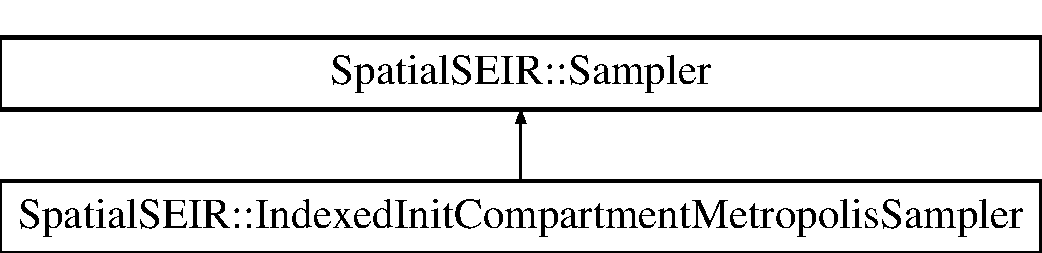
\includegraphics[height=2.000000cm]{classSpatialSEIR_1_1IndexedInitCompartmentMetropolisSampler}
\end{center}
\end{figure}
\subsection*{Public Member Functions}
\begin{DoxyCompactItemize}
\item 
\hyperlink{classSpatialSEIR_1_1IndexedInitCompartmentMetropolisSampler_aea5ccff0662970405b7db26aca1f5f45}{Indexed\-Init\-Compartment\-Metropolis\-Sampler} (\hyperlink{classSpatialSEIR_1_1ModelContext}{Model\-Context} $\ast$\hyperlink{classSpatialSEIR_1_1IndexedInitCompartmentMetropolisSampler_a9cd2c0c4c1ac2a2c22fd977d79756173}{context}, \hyperlink{classSpatialSEIR_1_1InitCompartmentFullConditional}{Init\-Compartment\-Full\-Conditional} $\ast$\hyperlink{classSpatialSEIR_1_1IndexedInitCompartmentMetropolisSampler_a8c747dd4513ff2df6e5780b2f00cc99b}{init\-Compartment\-F\-C}, int $\ast$\hyperlink{classSpatialSEIR_1_1IndexedInitCompartmentMetropolisSampler_a5da3f9b3df2693b8b87530c261385d46}{init\-Compartment\-Data})
\item 
void \hyperlink{classSpatialSEIR_1_1IndexedInitCompartmentMetropolisSampler_ad8ee467d7679fa760db613075c9e0db2}{draw\-Sample} ()
\item 
int \hyperlink{classSpatialSEIR_1_1IndexedInitCompartmentMetropolisSampler_af2891523864f89b9587205eaba4bd41a}{get\-Sampler\-Type} ()
\item 
\hyperlink{classSpatialSEIR_1_1IndexedInitCompartmentMetropolisSampler_a079202d336eac83a21bc515e7ce70b07}{$\sim$\-Indexed\-Init\-Compartment\-Metropolis\-Sampler} ()
\end{DoxyCompactItemize}
\subsection*{Public Attributes}
\begin{DoxyCompactItemize}
\item 
\hyperlink{classSpatialSEIR_1_1ModelContext}{Model\-Context} $\ast$$\ast$ \hyperlink{classSpatialSEIR_1_1IndexedInitCompartmentMetropolisSampler_a9cd2c0c4c1ac2a2c22fd977d79756173}{context}
\item 
\hyperlink{classSpatialSEIR_1_1InitCompartmentFullConditional}{Init\-Compartment\-Full\-Conditional} $\ast$$\ast$ \hyperlink{classSpatialSEIR_1_1IndexedInitCompartmentMetropolisSampler_a8c747dd4513ff2df6e5780b2f00cc99b}{init\-Compartment\-F\-C}
\item 
int $\ast$$\ast$ \hyperlink{classSpatialSEIR_1_1IndexedInitCompartmentMetropolisSampler_a41fc7cdd1c6907172dbf51609fe81470}{index\-Length}
\item 
int $\ast$$\ast$ \hyperlink{classSpatialSEIR_1_1IndexedInitCompartmentMetropolisSampler_adfb486cecdbbc3a605465e9ff709ae24}{index\-List}
\item 
int $\ast$$\ast$ \hyperlink{classSpatialSEIR_1_1IndexedInitCompartmentMetropolisSampler_a5da3f9b3df2693b8b87530c261385d46}{init\-Compartment\-Data}
\end{DoxyCompactItemize}


\subsection{Detailed Description}
The \hyperlink{classSpatialSEIR_1_1IndexedInitCompartmentMetropolisSampler}{Indexed\-Init\-Compartment\-Metropolis\-Sampler} is depricated. 

\subsection{Constructor \& Destructor Documentation}
\hypertarget{classSpatialSEIR_1_1IndexedInitCompartmentMetropolisSampler_aea5ccff0662970405b7db26aca1f5f45}{\index{Spatial\-S\-E\-I\-R\-::\-Indexed\-Init\-Compartment\-Metropolis\-Sampler@{Spatial\-S\-E\-I\-R\-::\-Indexed\-Init\-Compartment\-Metropolis\-Sampler}!Indexed\-Init\-Compartment\-Metropolis\-Sampler@{Indexed\-Init\-Compartment\-Metropolis\-Sampler}}
\index{Indexed\-Init\-Compartment\-Metropolis\-Sampler@{Indexed\-Init\-Compartment\-Metropolis\-Sampler}!SpatialSEIR::IndexedInitCompartmentMetropolisSampler@{Spatial\-S\-E\-I\-R\-::\-Indexed\-Init\-Compartment\-Metropolis\-Sampler}}
\subsubsection[{Indexed\-Init\-Compartment\-Metropolis\-Sampler}]{\setlength{\rightskip}{0pt plus 5cm}Spatial\-S\-E\-I\-R\-::\-Indexed\-Init\-Compartment\-Metropolis\-Sampler\-::\-Indexed\-Init\-Compartment\-Metropolis\-Sampler (
\begin{DoxyParamCaption}
\item[{{\bf Model\-Context} $\ast$}]{context, }
\item[{{\bf Init\-Compartment\-Full\-Conditional} $\ast$}]{init\-Compartment\-F\-C, }
\item[{int $\ast$}]{init\-Compartment\-Data}
\end{DoxyParamCaption}
)}}\label{classSpatialSEIR_1_1IndexedInitCompartmentMetropolisSampler_aea5ccff0662970405b7db26aca1f5f45}
\hypertarget{classSpatialSEIR_1_1IndexedInitCompartmentMetropolisSampler_a079202d336eac83a21bc515e7ce70b07}{\index{Spatial\-S\-E\-I\-R\-::\-Indexed\-Init\-Compartment\-Metropolis\-Sampler@{Spatial\-S\-E\-I\-R\-::\-Indexed\-Init\-Compartment\-Metropolis\-Sampler}!$\sim$\-Indexed\-Init\-Compartment\-Metropolis\-Sampler@{$\sim$\-Indexed\-Init\-Compartment\-Metropolis\-Sampler}}
\index{$\sim$\-Indexed\-Init\-Compartment\-Metropolis\-Sampler@{$\sim$\-Indexed\-Init\-Compartment\-Metropolis\-Sampler}!SpatialSEIR::IndexedInitCompartmentMetropolisSampler@{Spatial\-S\-E\-I\-R\-::\-Indexed\-Init\-Compartment\-Metropolis\-Sampler}}
\subsubsection[{$\sim$\-Indexed\-Init\-Compartment\-Metropolis\-Sampler}]{\setlength{\rightskip}{0pt plus 5cm}Spatial\-S\-E\-I\-R\-::\-Indexed\-Init\-Compartment\-Metropolis\-Sampler\-::$\sim$\-Indexed\-Init\-Compartment\-Metropolis\-Sampler (
\begin{DoxyParamCaption}
{}
\end{DoxyParamCaption}
)}}\label{classSpatialSEIR_1_1IndexedInitCompartmentMetropolisSampler_a079202d336eac83a21bc515e7ce70b07}


\subsection{Member Function Documentation}
\hypertarget{classSpatialSEIR_1_1IndexedInitCompartmentMetropolisSampler_ad8ee467d7679fa760db613075c9e0db2}{\index{Spatial\-S\-E\-I\-R\-::\-Indexed\-Init\-Compartment\-Metropolis\-Sampler@{Spatial\-S\-E\-I\-R\-::\-Indexed\-Init\-Compartment\-Metropolis\-Sampler}!draw\-Sample@{draw\-Sample}}
\index{draw\-Sample@{draw\-Sample}!SpatialSEIR::IndexedInitCompartmentMetropolisSampler@{Spatial\-S\-E\-I\-R\-::\-Indexed\-Init\-Compartment\-Metropolis\-Sampler}}
\subsubsection[{draw\-Sample}]{\setlength{\rightskip}{0pt plus 5cm}void Spatial\-S\-E\-I\-R\-::\-Indexed\-Init\-Compartment\-Metropolis\-Sampler\-::draw\-Sample (
\begin{DoxyParamCaption}
{}
\end{DoxyParamCaption}
)\hspace{0.3cm}{\ttfamily [virtual]}}}\label{classSpatialSEIR_1_1IndexedInitCompartmentMetropolisSampler_ad8ee467d7679fa760db613075c9e0db2}


Implements \hyperlink{classSpatialSEIR_1_1Sampler_aa07a42b26cb62249c20c58e855a08657}{Spatial\-S\-E\-I\-R\-::\-Sampler}.

\hypertarget{classSpatialSEIR_1_1IndexedInitCompartmentMetropolisSampler_af2891523864f89b9587205eaba4bd41a}{\index{Spatial\-S\-E\-I\-R\-::\-Indexed\-Init\-Compartment\-Metropolis\-Sampler@{Spatial\-S\-E\-I\-R\-::\-Indexed\-Init\-Compartment\-Metropolis\-Sampler}!get\-Sampler\-Type@{get\-Sampler\-Type}}
\index{get\-Sampler\-Type@{get\-Sampler\-Type}!SpatialSEIR::IndexedInitCompartmentMetropolisSampler@{Spatial\-S\-E\-I\-R\-::\-Indexed\-Init\-Compartment\-Metropolis\-Sampler}}
\subsubsection[{get\-Sampler\-Type}]{\setlength{\rightskip}{0pt plus 5cm}int Spatial\-S\-E\-I\-R\-::\-Indexed\-Init\-Compartment\-Metropolis\-Sampler\-::get\-Sampler\-Type (
\begin{DoxyParamCaption}
{}
\end{DoxyParamCaption}
)\hspace{0.3cm}{\ttfamily [virtual]}}}\label{classSpatialSEIR_1_1IndexedInitCompartmentMetropolisSampler_af2891523864f89b9587205eaba4bd41a}


Implements \hyperlink{classSpatialSEIR_1_1Sampler_aaa79310ad809e6aeb25479849f322dda}{Spatial\-S\-E\-I\-R\-::\-Sampler}.



\subsection{Member Data Documentation}
\hypertarget{classSpatialSEIR_1_1IndexedInitCompartmentMetropolisSampler_a9cd2c0c4c1ac2a2c22fd977d79756173}{\index{Spatial\-S\-E\-I\-R\-::\-Indexed\-Init\-Compartment\-Metropolis\-Sampler@{Spatial\-S\-E\-I\-R\-::\-Indexed\-Init\-Compartment\-Metropolis\-Sampler}!context@{context}}
\index{context@{context}!SpatialSEIR::IndexedInitCompartmentMetropolisSampler@{Spatial\-S\-E\-I\-R\-::\-Indexed\-Init\-Compartment\-Metropolis\-Sampler}}
\subsubsection[{context}]{\setlength{\rightskip}{0pt plus 5cm}{\bf Model\-Context}$\ast$$\ast$ Spatial\-S\-E\-I\-R\-::\-Indexed\-Init\-Compartment\-Metropolis\-Sampler\-::context}}\label{classSpatialSEIR_1_1IndexedInitCompartmentMetropolisSampler_a9cd2c0c4c1ac2a2c22fd977d79756173}
\hypertarget{classSpatialSEIR_1_1IndexedInitCompartmentMetropolisSampler_a41fc7cdd1c6907172dbf51609fe81470}{\index{Spatial\-S\-E\-I\-R\-::\-Indexed\-Init\-Compartment\-Metropolis\-Sampler@{Spatial\-S\-E\-I\-R\-::\-Indexed\-Init\-Compartment\-Metropolis\-Sampler}!index\-Length@{index\-Length}}
\index{index\-Length@{index\-Length}!SpatialSEIR::IndexedInitCompartmentMetropolisSampler@{Spatial\-S\-E\-I\-R\-::\-Indexed\-Init\-Compartment\-Metropolis\-Sampler}}
\subsubsection[{index\-Length}]{\setlength{\rightskip}{0pt plus 5cm}int$\ast$$\ast$ Spatial\-S\-E\-I\-R\-::\-Indexed\-Init\-Compartment\-Metropolis\-Sampler\-::index\-Length}}\label{classSpatialSEIR_1_1IndexedInitCompartmentMetropolisSampler_a41fc7cdd1c6907172dbf51609fe81470}
\hypertarget{classSpatialSEIR_1_1IndexedInitCompartmentMetropolisSampler_adfb486cecdbbc3a605465e9ff709ae24}{\index{Spatial\-S\-E\-I\-R\-::\-Indexed\-Init\-Compartment\-Metropolis\-Sampler@{Spatial\-S\-E\-I\-R\-::\-Indexed\-Init\-Compartment\-Metropolis\-Sampler}!index\-List@{index\-List}}
\index{index\-List@{index\-List}!SpatialSEIR::IndexedInitCompartmentMetropolisSampler@{Spatial\-S\-E\-I\-R\-::\-Indexed\-Init\-Compartment\-Metropolis\-Sampler}}
\subsubsection[{index\-List}]{\setlength{\rightskip}{0pt plus 5cm}int$\ast$$\ast$ Spatial\-S\-E\-I\-R\-::\-Indexed\-Init\-Compartment\-Metropolis\-Sampler\-::index\-List}}\label{classSpatialSEIR_1_1IndexedInitCompartmentMetropolisSampler_adfb486cecdbbc3a605465e9ff709ae24}
\hypertarget{classSpatialSEIR_1_1IndexedInitCompartmentMetropolisSampler_a5da3f9b3df2693b8b87530c261385d46}{\index{Spatial\-S\-E\-I\-R\-::\-Indexed\-Init\-Compartment\-Metropolis\-Sampler@{Spatial\-S\-E\-I\-R\-::\-Indexed\-Init\-Compartment\-Metropolis\-Sampler}!init\-Compartment\-Data@{init\-Compartment\-Data}}
\index{init\-Compartment\-Data@{init\-Compartment\-Data}!SpatialSEIR::IndexedInitCompartmentMetropolisSampler@{Spatial\-S\-E\-I\-R\-::\-Indexed\-Init\-Compartment\-Metropolis\-Sampler}}
\subsubsection[{init\-Compartment\-Data}]{\setlength{\rightskip}{0pt plus 5cm}int$\ast$$\ast$ Spatial\-S\-E\-I\-R\-::\-Indexed\-Init\-Compartment\-Metropolis\-Sampler\-::init\-Compartment\-Data}}\label{classSpatialSEIR_1_1IndexedInitCompartmentMetropolisSampler_a5da3f9b3df2693b8b87530c261385d46}
\hypertarget{classSpatialSEIR_1_1IndexedInitCompartmentMetropolisSampler_a8c747dd4513ff2df6e5780b2f00cc99b}{\index{Spatial\-S\-E\-I\-R\-::\-Indexed\-Init\-Compartment\-Metropolis\-Sampler@{Spatial\-S\-E\-I\-R\-::\-Indexed\-Init\-Compartment\-Metropolis\-Sampler}!init\-Compartment\-F\-C@{init\-Compartment\-F\-C}}
\index{init\-Compartment\-F\-C@{init\-Compartment\-F\-C}!SpatialSEIR::IndexedInitCompartmentMetropolisSampler@{Spatial\-S\-E\-I\-R\-::\-Indexed\-Init\-Compartment\-Metropolis\-Sampler}}
\subsubsection[{init\-Compartment\-F\-C}]{\setlength{\rightskip}{0pt plus 5cm}{\bf Init\-Compartment\-Full\-Conditional}$\ast$$\ast$ Spatial\-S\-E\-I\-R\-::\-Indexed\-Init\-Compartment\-Metropolis\-Sampler\-::init\-Compartment\-F\-C}}\label{classSpatialSEIR_1_1IndexedInitCompartmentMetropolisSampler_a8c747dd4513ff2df6e5780b2f00cc99b}


The documentation for this class was generated from the following file\-:\begin{DoxyCompactItemize}
\item 
lib\-Spatial\-S\-E\-I\-R/include/\hyperlink{LSS__Samplers_8hpp}{L\-S\-S\-\_\-\-Samplers.\-hpp}\end{DoxyCompactItemize}

\hypertarget{classSpatialSEIR_1_1IndexedInitCompartmentSliceSampler}{\section{Spatial\-S\-E\-I\-R\-:\-:Indexed\-Init\-Compartment\-Slice\-Sampler Class Reference}
\label{classSpatialSEIR_1_1IndexedInitCompartmentSliceSampler}\index{Spatial\-S\-E\-I\-R\-::\-Indexed\-Init\-Compartment\-Slice\-Sampler@{Spatial\-S\-E\-I\-R\-::\-Indexed\-Init\-Compartment\-Slice\-Sampler}}
}


{\ttfamily \#include $<$L\-S\-S\-\_\-\-Samplers.\-hpp$>$}

Inheritance diagram for Spatial\-S\-E\-I\-R\-:\-:Indexed\-Init\-Compartment\-Slice\-Sampler\-:\begin{figure}[H]
\begin{center}
\leavevmode
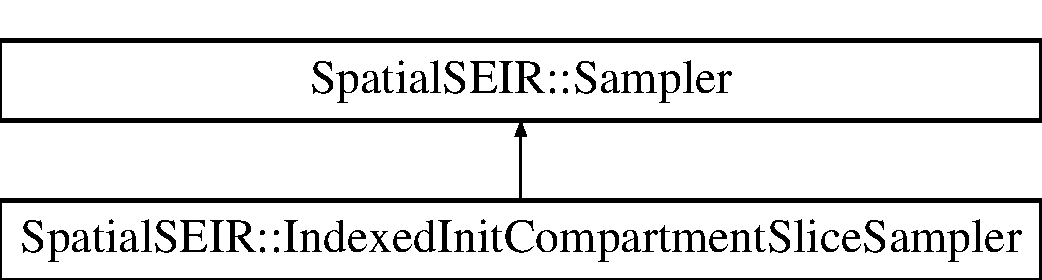
\includegraphics[height=2.000000cm]{classSpatialSEIR_1_1IndexedInitCompartmentSliceSampler}
\end{center}
\end{figure}
\subsection*{Public Member Functions}
\begin{DoxyCompactItemize}
\item 
\hyperlink{classSpatialSEIR_1_1IndexedInitCompartmentSliceSampler_aab73b27c283b18841da79a500f29fdeb}{Indexed\-Init\-Compartment\-Slice\-Sampler} (\hyperlink{classSpatialSEIR_1_1ModelContext}{Model\-Context} $\ast$\hyperlink{classSpatialSEIR_1_1IndexedInitCompartmentSliceSampler_aeaa9d7c11d3bb0000f236c95a2c8f041}{context}, \hyperlink{classSpatialSEIR_1_1InitCompartmentFullConditional}{Init\-Compartment\-Full\-Conditional} $\ast$\hyperlink{classSpatialSEIR_1_1IndexedInitCompartmentSliceSampler_a729e2d6ea861584920909fc54d3094f0}{init\-Compartment\-F\-C}, int $\ast$\hyperlink{classSpatialSEIR_1_1IndexedInitCompartmentSliceSampler_a8660c84e839a34b1a53cb16b9b53f66f}{init\-Compartment\-Data})
\item 
void \hyperlink{classSpatialSEIR_1_1IndexedInitCompartmentSliceSampler_a2ff3fc36c3cfc5b49c58234376ba0a1b}{draw\-Sample} ()
\item 
int \hyperlink{classSpatialSEIR_1_1IndexedInitCompartmentSliceSampler_a8687c4d1acc384cc4e8d7f4b91db79a5}{get\-Sampler\-Type} ()
\item 
\hyperlink{classSpatialSEIR_1_1IndexedInitCompartmentSliceSampler_ab7e3dd539f1d6f66cfbd7de31a10fbce}{$\sim$\-Indexed\-Init\-Compartment\-Slice\-Sampler} ()
\end{DoxyCompactItemize}
\subsection*{Public Attributes}
\begin{DoxyCompactItemize}
\item 
\hyperlink{classSpatialSEIR_1_1ModelContext}{Model\-Context} $\ast$$\ast$ \hyperlink{classSpatialSEIR_1_1IndexedInitCompartmentSliceSampler_aeaa9d7c11d3bb0000f236c95a2c8f041}{context}
\item 
\hyperlink{classSpatialSEIR_1_1InitCompartmentFullConditional}{Init\-Compartment\-Full\-Conditional} $\ast$$\ast$ \hyperlink{classSpatialSEIR_1_1IndexedInitCompartmentSliceSampler_a729e2d6ea861584920909fc54d3094f0}{init\-Compartment\-F\-C}
\item 
int $\ast$$\ast$ \hyperlink{classSpatialSEIR_1_1IndexedInitCompartmentSliceSampler_ae7e9d465efab1aff109ab06aa2ca703e}{index\-Length}
\item 
int $\ast$$\ast$ \hyperlink{classSpatialSEIR_1_1IndexedInitCompartmentSliceSampler_ac0ef023fbdf4e7b5e4afdaa112284b6c}{index\-List}
\item 
int $\ast$$\ast$ \hyperlink{classSpatialSEIR_1_1IndexedInitCompartmentSliceSampler_a8660c84e839a34b1a53cb16b9b53f66f}{init\-Compartment\-Data}
\end{DoxyCompactItemize}


\subsection{Detailed Description}
The \hyperlink{classSpatialSEIR_1_1IndexedInitCompartmentSliceSampler}{Indexed\-Init\-Compartment\-Slice\-Sampler} is depricated. 

\subsection{Constructor \& Destructor Documentation}
\hypertarget{classSpatialSEIR_1_1IndexedInitCompartmentSliceSampler_aab73b27c283b18841da79a500f29fdeb}{\index{Spatial\-S\-E\-I\-R\-::\-Indexed\-Init\-Compartment\-Slice\-Sampler@{Spatial\-S\-E\-I\-R\-::\-Indexed\-Init\-Compartment\-Slice\-Sampler}!Indexed\-Init\-Compartment\-Slice\-Sampler@{Indexed\-Init\-Compartment\-Slice\-Sampler}}
\index{Indexed\-Init\-Compartment\-Slice\-Sampler@{Indexed\-Init\-Compartment\-Slice\-Sampler}!SpatialSEIR::IndexedInitCompartmentSliceSampler@{Spatial\-S\-E\-I\-R\-::\-Indexed\-Init\-Compartment\-Slice\-Sampler}}
\subsubsection[{Indexed\-Init\-Compartment\-Slice\-Sampler}]{\setlength{\rightskip}{0pt plus 5cm}Spatial\-S\-E\-I\-R\-::\-Indexed\-Init\-Compartment\-Slice\-Sampler\-::\-Indexed\-Init\-Compartment\-Slice\-Sampler (
\begin{DoxyParamCaption}
\item[{{\bf Model\-Context} $\ast$}]{context, }
\item[{{\bf Init\-Compartment\-Full\-Conditional} $\ast$}]{init\-Compartment\-F\-C, }
\item[{int $\ast$}]{init\-Compartment\-Data}
\end{DoxyParamCaption}
)}}\label{classSpatialSEIR_1_1IndexedInitCompartmentSliceSampler_aab73b27c283b18841da79a500f29fdeb}
\hypertarget{classSpatialSEIR_1_1IndexedInitCompartmentSliceSampler_ab7e3dd539f1d6f66cfbd7de31a10fbce}{\index{Spatial\-S\-E\-I\-R\-::\-Indexed\-Init\-Compartment\-Slice\-Sampler@{Spatial\-S\-E\-I\-R\-::\-Indexed\-Init\-Compartment\-Slice\-Sampler}!$\sim$\-Indexed\-Init\-Compartment\-Slice\-Sampler@{$\sim$\-Indexed\-Init\-Compartment\-Slice\-Sampler}}
\index{$\sim$\-Indexed\-Init\-Compartment\-Slice\-Sampler@{$\sim$\-Indexed\-Init\-Compartment\-Slice\-Sampler}!SpatialSEIR::IndexedInitCompartmentSliceSampler@{Spatial\-S\-E\-I\-R\-::\-Indexed\-Init\-Compartment\-Slice\-Sampler}}
\subsubsection[{$\sim$\-Indexed\-Init\-Compartment\-Slice\-Sampler}]{\setlength{\rightskip}{0pt plus 5cm}Spatial\-S\-E\-I\-R\-::\-Indexed\-Init\-Compartment\-Slice\-Sampler\-::$\sim$\-Indexed\-Init\-Compartment\-Slice\-Sampler (
\begin{DoxyParamCaption}
{}
\end{DoxyParamCaption}
)}}\label{classSpatialSEIR_1_1IndexedInitCompartmentSliceSampler_ab7e3dd539f1d6f66cfbd7de31a10fbce}


\subsection{Member Function Documentation}
\hypertarget{classSpatialSEIR_1_1IndexedInitCompartmentSliceSampler_a2ff3fc36c3cfc5b49c58234376ba0a1b}{\index{Spatial\-S\-E\-I\-R\-::\-Indexed\-Init\-Compartment\-Slice\-Sampler@{Spatial\-S\-E\-I\-R\-::\-Indexed\-Init\-Compartment\-Slice\-Sampler}!draw\-Sample@{draw\-Sample}}
\index{draw\-Sample@{draw\-Sample}!SpatialSEIR::IndexedInitCompartmentSliceSampler@{Spatial\-S\-E\-I\-R\-::\-Indexed\-Init\-Compartment\-Slice\-Sampler}}
\subsubsection[{draw\-Sample}]{\setlength{\rightskip}{0pt plus 5cm}void Spatial\-S\-E\-I\-R\-::\-Indexed\-Init\-Compartment\-Slice\-Sampler\-::draw\-Sample (
\begin{DoxyParamCaption}
{}
\end{DoxyParamCaption}
)\hspace{0.3cm}{\ttfamily [virtual]}}}\label{classSpatialSEIR_1_1IndexedInitCompartmentSliceSampler_a2ff3fc36c3cfc5b49c58234376ba0a1b}


Implements \hyperlink{classSpatialSEIR_1_1Sampler_aa07a42b26cb62249c20c58e855a08657}{Spatial\-S\-E\-I\-R\-::\-Sampler}.

\hypertarget{classSpatialSEIR_1_1IndexedInitCompartmentSliceSampler_a8687c4d1acc384cc4e8d7f4b91db79a5}{\index{Spatial\-S\-E\-I\-R\-::\-Indexed\-Init\-Compartment\-Slice\-Sampler@{Spatial\-S\-E\-I\-R\-::\-Indexed\-Init\-Compartment\-Slice\-Sampler}!get\-Sampler\-Type@{get\-Sampler\-Type}}
\index{get\-Sampler\-Type@{get\-Sampler\-Type}!SpatialSEIR::IndexedInitCompartmentSliceSampler@{Spatial\-S\-E\-I\-R\-::\-Indexed\-Init\-Compartment\-Slice\-Sampler}}
\subsubsection[{get\-Sampler\-Type}]{\setlength{\rightskip}{0pt plus 5cm}int Spatial\-S\-E\-I\-R\-::\-Indexed\-Init\-Compartment\-Slice\-Sampler\-::get\-Sampler\-Type (
\begin{DoxyParamCaption}
{}
\end{DoxyParamCaption}
)\hspace{0.3cm}{\ttfamily [virtual]}}}\label{classSpatialSEIR_1_1IndexedInitCompartmentSliceSampler_a8687c4d1acc384cc4e8d7f4b91db79a5}


Implements \hyperlink{classSpatialSEIR_1_1Sampler_aaa79310ad809e6aeb25479849f322dda}{Spatial\-S\-E\-I\-R\-::\-Sampler}.



\subsection{Member Data Documentation}
\hypertarget{classSpatialSEIR_1_1IndexedInitCompartmentSliceSampler_aeaa9d7c11d3bb0000f236c95a2c8f041}{\index{Spatial\-S\-E\-I\-R\-::\-Indexed\-Init\-Compartment\-Slice\-Sampler@{Spatial\-S\-E\-I\-R\-::\-Indexed\-Init\-Compartment\-Slice\-Sampler}!context@{context}}
\index{context@{context}!SpatialSEIR::IndexedInitCompartmentSliceSampler@{Spatial\-S\-E\-I\-R\-::\-Indexed\-Init\-Compartment\-Slice\-Sampler}}
\subsubsection[{context}]{\setlength{\rightskip}{0pt plus 5cm}{\bf Model\-Context}$\ast$$\ast$ Spatial\-S\-E\-I\-R\-::\-Indexed\-Init\-Compartment\-Slice\-Sampler\-::context}}\label{classSpatialSEIR_1_1IndexedInitCompartmentSliceSampler_aeaa9d7c11d3bb0000f236c95a2c8f041}
\hypertarget{classSpatialSEIR_1_1IndexedInitCompartmentSliceSampler_ae7e9d465efab1aff109ab06aa2ca703e}{\index{Spatial\-S\-E\-I\-R\-::\-Indexed\-Init\-Compartment\-Slice\-Sampler@{Spatial\-S\-E\-I\-R\-::\-Indexed\-Init\-Compartment\-Slice\-Sampler}!index\-Length@{index\-Length}}
\index{index\-Length@{index\-Length}!SpatialSEIR::IndexedInitCompartmentSliceSampler@{Spatial\-S\-E\-I\-R\-::\-Indexed\-Init\-Compartment\-Slice\-Sampler}}
\subsubsection[{index\-Length}]{\setlength{\rightskip}{0pt plus 5cm}int$\ast$$\ast$ Spatial\-S\-E\-I\-R\-::\-Indexed\-Init\-Compartment\-Slice\-Sampler\-::index\-Length}}\label{classSpatialSEIR_1_1IndexedInitCompartmentSliceSampler_ae7e9d465efab1aff109ab06aa2ca703e}
\hypertarget{classSpatialSEIR_1_1IndexedInitCompartmentSliceSampler_ac0ef023fbdf4e7b5e4afdaa112284b6c}{\index{Spatial\-S\-E\-I\-R\-::\-Indexed\-Init\-Compartment\-Slice\-Sampler@{Spatial\-S\-E\-I\-R\-::\-Indexed\-Init\-Compartment\-Slice\-Sampler}!index\-List@{index\-List}}
\index{index\-List@{index\-List}!SpatialSEIR::IndexedInitCompartmentSliceSampler@{Spatial\-S\-E\-I\-R\-::\-Indexed\-Init\-Compartment\-Slice\-Sampler}}
\subsubsection[{index\-List}]{\setlength{\rightskip}{0pt plus 5cm}int$\ast$$\ast$ Spatial\-S\-E\-I\-R\-::\-Indexed\-Init\-Compartment\-Slice\-Sampler\-::index\-List}}\label{classSpatialSEIR_1_1IndexedInitCompartmentSliceSampler_ac0ef023fbdf4e7b5e4afdaa112284b6c}
\hypertarget{classSpatialSEIR_1_1IndexedInitCompartmentSliceSampler_a8660c84e839a34b1a53cb16b9b53f66f}{\index{Spatial\-S\-E\-I\-R\-::\-Indexed\-Init\-Compartment\-Slice\-Sampler@{Spatial\-S\-E\-I\-R\-::\-Indexed\-Init\-Compartment\-Slice\-Sampler}!init\-Compartment\-Data@{init\-Compartment\-Data}}
\index{init\-Compartment\-Data@{init\-Compartment\-Data}!SpatialSEIR::IndexedInitCompartmentSliceSampler@{Spatial\-S\-E\-I\-R\-::\-Indexed\-Init\-Compartment\-Slice\-Sampler}}
\subsubsection[{init\-Compartment\-Data}]{\setlength{\rightskip}{0pt plus 5cm}int$\ast$$\ast$ Spatial\-S\-E\-I\-R\-::\-Indexed\-Init\-Compartment\-Slice\-Sampler\-::init\-Compartment\-Data}}\label{classSpatialSEIR_1_1IndexedInitCompartmentSliceSampler_a8660c84e839a34b1a53cb16b9b53f66f}
\hypertarget{classSpatialSEIR_1_1IndexedInitCompartmentSliceSampler_a729e2d6ea861584920909fc54d3094f0}{\index{Spatial\-S\-E\-I\-R\-::\-Indexed\-Init\-Compartment\-Slice\-Sampler@{Spatial\-S\-E\-I\-R\-::\-Indexed\-Init\-Compartment\-Slice\-Sampler}!init\-Compartment\-F\-C@{init\-Compartment\-F\-C}}
\index{init\-Compartment\-F\-C@{init\-Compartment\-F\-C}!SpatialSEIR::IndexedInitCompartmentSliceSampler@{Spatial\-S\-E\-I\-R\-::\-Indexed\-Init\-Compartment\-Slice\-Sampler}}
\subsubsection[{init\-Compartment\-F\-C}]{\setlength{\rightskip}{0pt plus 5cm}{\bf Init\-Compartment\-Full\-Conditional}$\ast$$\ast$ Spatial\-S\-E\-I\-R\-::\-Indexed\-Init\-Compartment\-Slice\-Sampler\-::init\-Compartment\-F\-C}}\label{classSpatialSEIR_1_1IndexedInitCompartmentSliceSampler_a729e2d6ea861584920909fc54d3094f0}


The documentation for this class was generated from the following file\-:\begin{DoxyCompactItemize}
\item 
lib\-Spatial\-S\-E\-I\-R/include/\hyperlink{LSS__Samplers_8hpp}{L\-S\-S\-\_\-\-Samplers.\-hpp}\end{DoxyCompactItemize}

\hypertarget{classSpatialSEIR_1_1InitCompartmentFullConditional}{\section{Spatial\-S\-E\-I\-R\-:\-:Init\-Compartment\-Full\-Conditional Class Reference}
\label{classSpatialSEIR_1_1InitCompartmentFullConditional}\index{Spatial\-S\-E\-I\-R\-::\-Init\-Compartment\-Full\-Conditional@{Spatial\-S\-E\-I\-R\-::\-Init\-Compartment\-Full\-Conditional}}
}


{\ttfamily \#include $<$L\-S\-S\-\_\-\-Full\-Conditional.\-hpp$>$}

Inheritance diagram for Spatial\-S\-E\-I\-R\-:\-:Init\-Compartment\-Full\-Conditional\-:\begin{figure}[H]
\begin{center}
\leavevmode
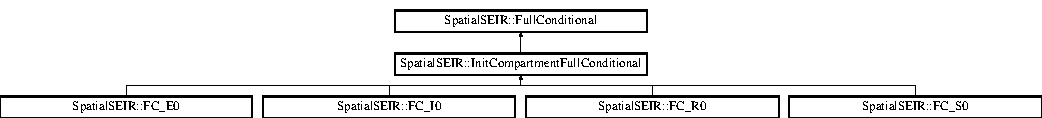
\includegraphics[height=1.590909cm]{classSpatialSEIR_1_1InitCompartmentFullConditional}
\end{center}
\end{figure}
\subsection*{Public Member Functions}
\begin{DoxyCompactItemize}
\item 
virtual \hyperlink{classSpatialSEIR_1_1InitCompartmentFullConditional_a4d1e4214653686f98dbe94809e6a8390}{$\sim$\-Init\-Compartment\-Full\-Conditional} ()
\item 
virtual int \hyperlink{classSpatialSEIR_1_1InitCompartmentFullConditional_a25fc6e3ac2cb71a6e115ce3235fd8de0}{eval\-C\-P\-U} ()=0
\item 
virtual int \hyperlink{classSpatialSEIR_1_1InitCompartmentFullConditional_a2f0c4b5628e2f2074c1a84ea6349a754}{eval\-O\-C\-L} ()=0
\item 
virtual void \hyperlink{classSpatialSEIR_1_1InitCompartmentFullConditional_a03bcc440fa87265336980f3e833f59f2}{sample} (int verbose)=0
\item 
virtual long double \hyperlink{classSpatialSEIR_1_1InitCompartmentFullConditional_aadb3975a791221136e6c4be5e016d9f1}{get\-Value} ()=0
\item 
virtual void \hyperlink{classSpatialSEIR_1_1InitCompartmentFullConditional_acbc03a68f5c67beacefadcc3c22c1d88}{set\-Value} (long double value)=0
\item 
virtual int \hyperlink{classSpatialSEIR_1_1InitCompartmentFullConditional_a3fab33c4f5b857998fd928a00cea09e7}{calculate\-Relevant\-Compartments} ()=0
\item 
virtual int \hyperlink{classSpatialSEIR_1_1InitCompartmentFullConditional_aa4eae1aafbcdc4819be2e520d600dedf}{calculate\-Relevant\-Compartments\-\_\-\-O\-C\-L} ()=0
\item 
void \hyperlink{classSpatialSEIR_1_1InitCompartmentFullConditional_a7cf7ddd043ec51b17a3c369ebe03a95c}{update\-Sampling\-Parameters} (double desired\-Ratio, double target\-Width, double proportion\-Change)
\item 
int \hyperlink{classSpatialSEIR_1_1InitCompartmentFullConditional_a6c35c9ed95a8adbada0e3da0608531bd}{get\-Full\-Conditional\-Type} ()
\end{DoxyCompactItemize}
\subsection*{Additional Inherited Members}


\subsection{Detailed Description}
The \hyperlink{classSpatialSEIR_1_1InitCompartmentFullConditional}{Init\-Compartment\-Full\-Conditional} class inherits the structure of \hyperlink{classSpatialSEIR_1_1FullConditional}{Full\-Conditional}, and provides sampling methods for the initial compartment size parameters. These are\-:
\begin{DoxyEnumerate}
\item \hyperlink{classSpatialSEIR_1_1FC__S0}{F\-C\-\_\-\-S0}, the initial susceptible group
\item \hyperlink{classSpatialSEIR_1_1FC__E0}{F\-C\-\_\-\-E0}, the initial exposed group
\item \hyperlink{classSpatialSEIR_1_1FC__I0}{F\-C\-\_\-\-I0}, the initial infectious group
\item \hyperlink{classSpatialSEIR_1_1FC__R0}{F\-C\-\_\-\-R0}, the initial recovered group 
\end{DoxyEnumerate}

\subsection{Constructor \& Destructor Documentation}
\hypertarget{classSpatialSEIR_1_1InitCompartmentFullConditional_a4d1e4214653686f98dbe94809e6a8390}{\index{Spatial\-S\-E\-I\-R\-::\-Init\-Compartment\-Full\-Conditional@{Spatial\-S\-E\-I\-R\-::\-Init\-Compartment\-Full\-Conditional}!$\sim$\-Init\-Compartment\-Full\-Conditional@{$\sim$\-Init\-Compartment\-Full\-Conditional}}
\index{$\sim$\-Init\-Compartment\-Full\-Conditional@{$\sim$\-Init\-Compartment\-Full\-Conditional}!SpatialSEIR::InitCompartmentFullConditional@{Spatial\-S\-E\-I\-R\-::\-Init\-Compartment\-Full\-Conditional}}
\subsubsection[{$\sim$\-Init\-Compartment\-Full\-Conditional}]{\setlength{\rightskip}{0pt plus 5cm}virtual Spatial\-S\-E\-I\-R\-::\-Init\-Compartment\-Full\-Conditional\-::$\sim$\-Init\-Compartment\-Full\-Conditional (
\begin{DoxyParamCaption}
{}
\end{DoxyParamCaption}
)\hspace{0.3cm}{\ttfamily [inline]}, {\ttfamily [virtual]}}}\label{classSpatialSEIR_1_1InitCompartmentFullConditional_a4d1e4214653686f98dbe94809e6a8390}


\subsection{Member Function Documentation}
\hypertarget{classSpatialSEIR_1_1InitCompartmentFullConditional_a3fab33c4f5b857998fd928a00cea09e7}{\index{Spatial\-S\-E\-I\-R\-::\-Init\-Compartment\-Full\-Conditional@{Spatial\-S\-E\-I\-R\-::\-Init\-Compartment\-Full\-Conditional}!calculate\-Relevant\-Compartments@{calculate\-Relevant\-Compartments}}
\index{calculate\-Relevant\-Compartments@{calculate\-Relevant\-Compartments}!SpatialSEIR::InitCompartmentFullConditional@{Spatial\-S\-E\-I\-R\-::\-Init\-Compartment\-Full\-Conditional}}
\subsubsection[{calculate\-Relevant\-Compartments}]{\setlength{\rightskip}{0pt plus 5cm}virtual int Spatial\-S\-E\-I\-R\-::\-Init\-Compartment\-Full\-Conditional\-::calculate\-Relevant\-Compartments (
\begin{DoxyParamCaption}
{}
\end{DoxyParamCaption}
)\hspace{0.3cm}{\ttfamily [pure virtual]}}}\label{classSpatialSEIR_1_1InitCompartmentFullConditional_a3fab33c4f5b857998fd928a00cea09e7}


Implements \hyperlink{classSpatialSEIR_1_1FullConditional_a04c671e900a359f5a554817f21a99b5c}{Spatial\-S\-E\-I\-R\-::\-Full\-Conditional}.



Implemented in \hyperlink{classSpatialSEIR_1_1FC__I0_aa463dde280304445e22a9653536a1edb}{Spatial\-S\-E\-I\-R\-::\-F\-C\-\_\-\-I0}, \hyperlink{classSpatialSEIR_1_1FC__E0_accae19c302cdd306fdfebf3a76c84c11}{Spatial\-S\-E\-I\-R\-::\-F\-C\-\_\-\-E0}, \hyperlink{classSpatialSEIR_1_1FC__R0_a651e144af6767ba90b59ae04f3164c28}{Spatial\-S\-E\-I\-R\-::\-F\-C\-\_\-\-R0}, and \hyperlink{classSpatialSEIR_1_1FC__S0_a755fc8e1d69791f6f3883f12a2f1b1c9}{Spatial\-S\-E\-I\-R\-::\-F\-C\-\_\-\-S0}.

\hypertarget{classSpatialSEIR_1_1InitCompartmentFullConditional_aa4eae1aafbcdc4819be2e520d600dedf}{\index{Spatial\-S\-E\-I\-R\-::\-Init\-Compartment\-Full\-Conditional@{Spatial\-S\-E\-I\-R\-::\-Init\-Compartment\-Full\-Conditional}!calculate\-Relevant\-Compartments\-\_\-\-O\-C\-L@{calculate\-Relevant\-Compartments\-\_\-\-O\-C\-L}}
\index{calculate\-Relevant\-Compartments\-\_\-\-O\-C\-L@{calculate\-Relevant\-Compartments\-\_\-\-O\-C\-L}!SpatialSEIR::InitCompartmentFullConditional@{Spatial\-S\-E\-I\-R\-::\-Init\-Compartment\-Full\-Conditional}}
\subsubsection[{calculate\-Relevant\-Compartments\-\_\-\-O\-C\-L}]{\setlength{\rightskip}{0pt plus 5cm}virtual int Spatial\-S\-E\-I\-R\-::\-Init\-Compartment\-Full\-Conditional\-::calculate\-Relevant\-Compartments\-\_\-\-O\-C\-L (
\begin{DoxyParamCaption}
{}
\end{DoxyParamCaption}
)\hspace{0.3cm}{\ttfamily [pure virtual]}}}\label{classSpatialSEIR_1_1InitCompartmentFullConditional_aa4eae1aafbcdc4819be2e520d600dedf}


Implements \hyperlink{classSpatialSEIR_1_1FullConditional_a77b75e8e1f62175aa0380a2e9aca3d46}{Spatial\-S\-E\-I\-R\-::\-Full\-Conditional}.



Implemented in \hyperlink{classSpatialSEIR_1_1FC__I0_ab1d7728b636f695a984ce609de87efde}{Spatial\-S\-E\-I\-R\-::\-F\-C\-\_\-\-I0}, \hyperlink{classSpatialSEIR_1_1FC__E0_aab40abc211ff8095a6ed0ec0b0c48b51}{Spatial\-S\-E\-I\-R\-::\-F\-C\-\_\-\-E0}, \hyperlink{classSpatialSEIR_1_1FC__R0_ad94da8ac1a1b746f1902e709d4f81634}{Spatial\-S\-E\-I\-R\-::\-F\-C\-\_\-\-R0}, and \hyperlink{classSpatialSEIR_1_1FC__S0_ab1c67b9f867ed1e8b9ac27c4f855a102}{Spatial\-S\-E\-I\-R\-::\-F\-C\-\_\-\-S0}.

\hypertarget{classSpatialSEIR_1_1InitCompartmentFullConditional_a25fc6e3ac2cb71a6e115ce3235fd8de0}{\index{Spatial\-S\-E\-I\-R\-::\-Init\-Compartment\-Full\-Conditional@{Spatial\-S\-E\-I\-R\-::\-Init\-Compartment\-Full\-Conditional}!eval\-C\-P\-U@{eval\-C\-P\-U}}
\index{eval\-C\-P\-U@{eval\-C\-P\-U}!SpatialSEIR::InitCompartmentFullConditional@{Spatial\-S\-E\-I\-R\-::\-Init\-Compartment\-Full\-Conditional}}
\subsubsection[{eval\-C\-P\-U}]{\setlength{\rightskip}{0pt plus 5cm}virtual int Spatial\-S\-E\-I\-R\-::\-Init\-Compartment\-Full\-Conditional\-::eval\-C\-P\-U (
\begin{DoxyParamCaption}
{}
\end{DoxyParamCaption}
)\hspace{0.3cm}{\ttfamily [pure virtual]}}}\label{classSpatialSEIR_1_1InitCompartmentFullConditional_a25fc6e3ac2cb71a6e115ce3235fd8de0}


Implemented in \hyperlink{classSpatialSEIR_1_1FC__I0_a36dbaf498cb226c7b2042438f9432ae4}{Spatial\-S\-E\-I\-R\-::\-F\-C\-\_\-\-I0}, \hyperlink{classSpatialSEIR_1_1FC__E0_a6f38f6b04084d8cc9a94a360195e459c}{Spatial\-S\-E\-I\-R\-::\-F\-C\-\_\-\-E0}, \hyperlink{classSpatialSEIR_1_1FC__R0_a0a7321f7437898caad90229e67ce7e12}{Spatial\-S\-E\-I\-R\-::\-F\-C\-\_\-\-R0}, and \hyperlink{classSpatialSEIR_1_1FC__S0_ae52c137dbd299a31a1b2055e924c93c2}{Spatial\-S\-E\-I\-R\-::\-F\-C\-\_\-\-S0}.

\hypertarget{classSpatialSEIR_1_1InitCompartmentFullConditional_a2f0c4b5628e2f2074c1a84ea6349a754}{\index{Spatial\-S\-E\-I\-R\-::\-Init\-Compartment\-Full\-Conditional@{Spatial\-S\-E\-I\-R\-::\-Init\-Compartment\-Full\-Conditional}!eval\-O\-C\-L@{eval\-O\-C\-L}}
\index{eval\-O\-C\-L@{eval\-O\-C\-L}!SpatialSEIR::InitCompartmentFullConditional@{Spatial\-S\-E\-I\-R\-::\-Init\-Compartment\-Full\-Conditional}}
\subsubsection[{eval\-O\-C\-L}]{\setlength{\rightskip}{0pt plus 5cm}virtual int Spatial\-S\-E\-I\-R\-::\-Init\-Compartment\-Full\-Conditional\-::eval\-O\-C\-L (
\begin{DoxyParamCaption}
{}
\end{DoxyParamCaption}
)\hspace{0.3cm}{\ttfamily [pure virtual]}}}\label{classSpatialSEIR_1_1InitCompartmentFullConditional_a2f0c4b5628e2f2074c1a84ea6349a754}


Implemented in \hyperlink{classSpatialSEIR_1_1FC__I0_abc02f4b767cda97f040e53095dd3024d}{Spatial\-S\-E\-I\-R\-::\-F\-C\-\_\-\-I0}, \hyperlink{classSpatialSEIR_1_1FC__E0_a7470507101e662f3f0c1b1a6ab861089}{Spatial\-S\-E\-I\-R\-::\-F\-C\-\_\-\-E0}, \hyperlink{classSpatialSEIR_1_1FC__R0_a36373b69de6603391aceb7c326b2cc00}{Spatial\-S\-E\-I\-R\-::\-F\-C\-\_\-\-R0}, and \hyperlink{classSpatialSEIR_1_1FC__S0_a9f9e3df7a26de238959461dd6d2511ef}{Spatial\-S\-E\-I\-R\-::\-F\-C\-\_\-\-S0}.

\hypertarget{classSpatialSEIR_1_1InitCompartmentFullConditional_a6c35c9ed95a8adbada0e3da0608531bd}{\index{Spatial\-S\-E\-I\-R\-::\-Init\-Compartment\-Full\-Conditional@{Spatial\-S\-E\-I\-R\-::\-Init\-Compartment\-Full\-Conditional}!get\-Full\-Conditional\-Type@{get\-Full\-Conditional\-Type}}
\index{get\-Full\-Conditional\-Type@{get\-Full\-Conditional\-Type}!SpatialSEIR::InitCompartmentFullConditional@{Spatial\-S\-E\-I\-R\-::\-Init\-Compartment\-Full\-Conditional}}
\subsubsection[{get\-Full\-Conditional\-Type}]{\setlength{\rightskip}{0pt plus 5cm}int Spatial\-S\-E\-I\-R\-::\-Init\-Compartment\-Full\-Conditional\-::get\-Full\-Conditional\-Type (
\begin{DoxyParamCaption}
{}
\end{DoxyParamCaption}
)\hspace{0.3cm}{\ttfamily [virtual]}}}\label{classSpatialSEIR_1_1InitCompartmentFullConditional_a6c35c9ed95a8adbada0e3da0608531bd}
Identify as init compartment full conditional 

Implements \hyperlink{classSpatialSEIR_1_1FullConditional_a680a2a8af1962a5a99191ff84acf78c5}{Spatial\-S\-E\-I\-R\-::\-Full\-Conditional}.

\hypertarget{classSpatialSEIR_1_1InitCompartmentFullConditional_aadb3975a791221136e6c4be5e016d9f1}{\index{Spatial\-S\-E\-I\-R\-::\-Init\-Compartment\-Full\-Conditional@{Spatial\-S\-E\-I\-R\-::\-Init\-Compartment\-Full\-Conditional}!get\-Value@{get\-Value}}
\index{get\-Value@{get\-Value}!SpatialSEIR::InitCompartmentFullConditional@{Spatial\-S\-E\-I\-R\-::\-Init\-Compartment\-Full\-Conditional}}
\subsubsection[{get\-Value}]{\setlength{\rightskip}{0pt plus 5cm}virtual long double Spatial\-S\-E\-I\-R\-::\-Init\-Compartment\-Full\-Conditional\-::get\-Value (
\begin{DoxyParamCaption}
{}
\end{DoxyParamCaption}
)\hspace{0.3cm}{\ttfamily [pure virtual]}}}\label{classSpatialSEIR_1_1InitCompartmentFullConditional_aadb3975a791221136e6c4be5e016d9f1}


Implements \hyperlink{classSpatialSEIR_1_1FullConditional_abe67c774a66370686ee9dc6fe6f278f6}{Spatial\-S\-E\-I\-R\-::\-Full\-Conditional}.



Implemented in \hyperlink{classSpatialSEIR_1_1FC__I0_a69f4e641113c47ae2e28dbd44f8c8261}{Spatial\-S\-E\-I\-R\-::\-F\-C\-\_\-\-I0}, \hyperlink{classSpatialSEIR_1_1FC__E0_aa2681b2dc4378d162dd2c68ff5333288}{Spatial\-S\-E\-I\-R\-::\-F\-C\-\_\-\-E0}, \hyperlink{classSpatialSEIR_1_1FC__R0_ab52e48b7be8eb46258602b0d1467ff08}{Spatial\-S\-E\-I\-R\-::\-F\-C\-\_\-\-R0}, and \hyperlink{classSpatialSEIR_1_1FC__S0_ad1b806dbe3573b1e9652850b934d7b10}{Spatial\-S\-E\-I\-R\-::\-F\-C\-\_\-\-S0}.

\hypertarget{classSpatialSEIR_1_1InitCompartmentFullConditional_a03bcc440fa87265336980f3e833f59f2}{\index{Spatial\-S\-E\-I\-R\-::\-Init\-Compartment\-Full\-Conditional@{Spatial\-S\-E\-I\-R\-::\-Init\-Compartment\-Full\-Conditional}!sample@{sample}}
\index{sample@{sample}!SpatialSEIR::InitCompartmentFullConditional@{Spatial\-S\-E\-I\-R\-::\-Init\-Compartment\-Full\-Conditional}}
\subsubsection[{sample}]{\setlength{\rightskip}{0pt plus 5cm}virtual void Spatial\-S\-E\-I\-R\-::\-Init\-Compartment\-Full\-Conditional\-::sample (
\begin{DoxyParamCaption}
\item[{int}]{verbose}
\end{DoxyParamCaption}
)\hspace{0.3cm}{\ttfamily [pure virtual]}}}\label{classSpatialSEIR_1_1InitCompartmentFullConditional_a03bcc440fa87265336980f3e833f59f2}


Implements \hyperlink{classSpatialSEIR_1_1FullConditional_aac6928c9c2753acfc2c9e9bbe840ba82}{Spatial\-S\-E\-I\-R\-::\-Full\-Conditional}.



Implemented in \hyperlink{classSpatialSEIR_1_1FC__I0_af87aa3379ff282e36478301ff271ba40}{Spatial\-S\-E\-I\-R\-::\-F\-C\-\_\-\-I0}, \hyperlink{classSpatialSEIR_1_1FC__E0_a7b396dca06e12a96473d3bf2855a9dc7}{Spatial\-S\-E\-I\-R\-::\-F\-C\-\_\-\-E0}, \hyperlink{classSpatialSEIR_1_1FC__R0_afee9585fb8a21f38002912896c85b529}{Spatial\-S\-E\-I\-R\-::\-F\-C\-\_\-\-R0}, and \hyperlink{classSpatialSEIR_1_1FC__S0_a595cb5eceaa9ede016e1f1d341105de6}{Spatial\-S\-E\-I\-R\-::\-F\-C\-\_\-\-S0}.

\hypertarget{classSpatialSEIR_1_1InitCompartmentFullConditional_acbc03a68f5c67beacefadcc3c22c1d88}{\index{Spatial\-S\-E\-I\-R\-::\-Init\-Compartment\-Full\-Conditional@{Spatial\-S\-E\-I\-R\-::\-Init\-Compartment\-Full\-Conditional}!set\-Value@{set\-Value}}
\index{set\-Value@{set\-Value}!SpatialSEIR::InitCompartmentFullConditional@{Spatial\-S\-E\-I\-R\-::\-Init\-Compartment\-Full\-Conditional}}
\subsubsection[{set\-Value}]{\setlength{\rightskip}{0pt plus 5cm}virtual void Spatial\-S\-E\-I\-R\-::\-Init\-Compartment\-Full\-Conditional\-::set\-Value (
\begin{DoxyParamCaption}
\item[{long double}]{value}
\end{DoxyParamCaption}
)\hspace{0.3cm}{\ttfamily [pure virtual]}}}\label{classSpatialSEIR_1_1InitCompartmentFullConditional_acbc03a68f5c67beacefadcc3c22c1d88}


Implements \hyperlink{classSpatialSEIR_1_1FullConditional_a0834b0bb81ef4f7f368ba87fd784ff39}{Spatial\-S\-E\-I\-R\-::\-Full\-Conditional}.



Implemented in \hyperlink{classSpatialSEIR_1_1FC__I0_ae5db486bbdcdf2900278a17aea761e7a}{Spatial\-S\-E\-I\-R\-::\-F\-C\-\_\-\-I0}, \hyperlink{classSpatialSEIR_1_1FC__E0_a44355906ac90df5dff3e0b7ffc62e23b}{Spatial\-S\-E\-I\-R\-::\-F\-C\-\_\-\-E0}, \hyperlink{classSpatialSEIR_1_1FC__R0_a6b21261ddd1928e70dfea6ef25d553bd}{Spatial\-S\-E\-I\-R\-::\-F\-C\-\_\-\-R0}, and \hyperlink{classSpatialSEIR_1_1FC__S0_affd898a5e578d7efec9f133f5031cf13}{Spatial\-S\-E\-I\-R\-::\-F\-C\-\_\-\-S0}.

\hypertarget{classSpatialSEIR_1_1InitCompartmentFullConditional_a7cf7ddd043ec51b17a3c369ebe03a95c}{\index{Spatial\-S\-E\-I\-R\-::\-Init\-Compartment\-Full\-Conditional@{Spatial\-S\-E\-I\-R\-::\-Init\-Compartment\-Full\-Conditional}!update\-Sampling\-Parameters@{update\-Sampling\-Parameters}}
\index{update\-Sampling\-Parameters@{update\-Sampling\-Parameters}!SpatialSEIR::InitCompartmentFullConditional@{Spatial\-S\-E\-I\-R\-::\-Init\-Compartment\-Full\-Conditional}}
\subsubsection[{update\-Sampling\-Parameters}]{\setlength{\rightskip}{0pt plus 5cm}void Spatial\-S\-E\-I\-R\-::\-Init\-Compartment\-Full\-Conditional\-::update\-Sampling\-Parameters (
\begin{DoxyParamCaption}
\item[{double}]{desired\-Ratio, }
\item[{double}]{target\-Width, }
\item[{double}]{proportion\-Change}
\end{DoxyParamCaption}
)\hspace{0.3cm}{\ttfamily [virtual]}}}\label{classSpatialSEIR_1_1InitCompartmentFullConditional_a7cf7ddd043ec51b17a3c369ebe03a95c}


Implements \hyperlink{classSpatialSEIR_1_1FullConditional_afd84b9273d641028453aefc06b342782}{Spatial\-S\-E\-I\-R\-::\-Full\-Conditional}.



The documentation for this class was generated from the following files\-:\begin{DoxyCompactItemize}
\item 
lib\-Spatial\-S\-E\-I\-R/include/\-Full\-Conditionals/\hyperlink{LSS__FullConditional_8hpp}{L\-S\-S\-\_\-\-Full\-Conditional.\-hpp}\item 
lib\-Spatial\-S\-E\-I\-R/src/\-Full\-Conditionals/\hyperlink{FullConditional_8cpp}{Full\-Conditional.\-cpp}\end{DoxyCompactItemize}

\hypertarget{classSpatialSEIR_1_1InitCompartmentMetropolisSampler}{\section{Spatial\-S\-E\-I\-R\-:\-:Init\-Compartment\-Metropolis\-Sampler Class Reference}
\label{classSpatialSEIR_1_1InitCompartmentMetropolisSampler}\index{Spatial\-S\-E\-I\-R\-::\-Init\-Compartment\-Metropolis\-Sampler@{Spatial\-S\-E\-I\-R\-::\-Init\-Compartment\-Metropolis\-Sampler}}
}


{\ttfamily \#include $<$L\-S\-S\-\_\-\-Samplers.\-hpp$>$}

Inheritance diagram for Spatial\-S\-E\-I\-R\-:\-:Init\-Compartment\-Metropolis\-Sampler\-:\begin{figure}[H]
\begin{center}
\leavevmode
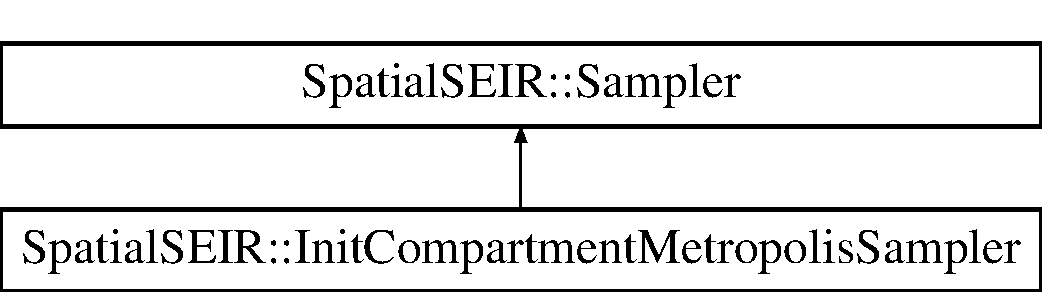
\includegraphics[height=2.000000cm]{classSpatialSEIR_1_1InitCompartmentMetropolisSampler}
\end{center}
\end{figure}
\subsection*{Public Member Functions}
\begin{DoxyCompactItemize}
\item 
\hyperlink{classSpatialSEIR_1_1InitCompartmentMetropolisSampler_a90228456741e4904deb02df3d74f27ed}{Init\-Compartment\-Metropolis\-Sampler} (\hyperlink{classSpatialSEIR_1_1ModelContext}{Model\-Context} $\ast$\hyperlink{classSpatialSEIR_1_1InitCompartmentMetropolisSampler_a3d6e255eb92808635a3b3cf869f136d8}{context}, \hyperlink{classSpatialSEIR_1_1InitCompartmentFullConditional}{Init\-Compartment\-Full\-Conditional} $\ast$\hyperlink{classSpatialSEIR_1_1InitCompartmentMetropolisSampler_af03f0584b11639e8fbe907307ad28aa4}{init\-Compartment\-F\-C}, int $\ast$\hyperlink{classSpatialSEIR_1_1InitCompartmentMetropolisSampler_ade210e4e15fddcfac80ce9c6c263e289}{init\-Compartment\-Data})
\item 
void \hyperlink{classSpatialSEIR_1_1InitCompartmentMetropolisSampler_a24aba18be0f06df089897aa471aa8a86}{draw\-Sample} ()
\item 
int \hyperlink{classSpatialSEIR_1_1InitCompartmentMetropolisSampler_ad64b5ae0943c980f752c49f9c179a3b7}{get\-Sampler\-Type} ()
\item 
\hyperlink{classSpatialSEIR_1_1InitCompartmentMetropolisSampler_ae09e31e0811fc8f531b54490e98a17ee}{$\sim$\-Init\-Compartment\-Metropolis\-Sampler} ()
\end{DoxyCompactItemize}
\subsection*{Public Attributes}
\begin{DoxyCompactItemize}
\item 
\hyperlink{classSpatialSEIR_1_1ModelContext}{Model\-Context} $\ast$$\ast$ \hyperlink{classSpatialSEIR_1_1InitCompartmentMetropolisSampler_a3d6e255eb92808635a3b3cf869f136d8}{context}
\item 
\hyperlink{classSpatialSEIR_1_1InitCompartmentFullConditional}{Init\-Compartment\-Full\-Conditional} $\ast$$\ast$ \hyperlink{classSpatialSEIR_1_1InitCompartmentMetropolisSampler_af03f0584b11639e8fbe907307ad28aa4}{init\-Compartment\-F\-C}
\item 
int $\ast$$\ast$ \hyperlink{classSpatialSEIR_1_1InitCompartmentMetropolisSampler_ade210e4e15fddcfac80ce9c6c263e289}{init\-Compartment\-Data}
\end{DoxyCompactItemize}


\subsection{Detailed Description}
The \hyperlink{classSpatialSEIR_1_1InitCompartmentMetropolisSampler}{Init\-Compartment\-Metropolis\-Sampler} functions identically to the \hyperlink{classSpatialSEIR_1_1CompartmentMetropolisSampler}{Compartment\-Metropolis\-Sampler} class, but for the vector of initial values of each \hyperlink{classSpatialSEIR_1_1CompartmentalModelMatrix}{Compartmental\-Model\-Matrix}. 

\subsection{Constructor \& Destructor Documentation}
\hypertarget{classSpatialSEIR_1_1InitCompartmentMetropolisSampler_a90228456741e4904deb02df3d74f27ed}{\index{Spatial\-S\-E\-I\-R\-::\-Init\-Compartment\-Metropolis\-Sampler@{Spatial\-S\-E\-I\-R\-::\-Init\-Compartment\-Metropolis\-Sampler}!Init\-Compartment\-Metropolis\-Sampler@{Init\-Compartment\-Metropolis\-Sampler}}
\index{Init\-Compartment\-Metropolis\-Sampler@{Init\-Compartment\-Metropolis\-Sampler}!SpatialSEIR::InitCompartmentMetropolisSampler@{Spatial\-S\-E\-I\-R\-::\-Init\-Compartment\-Metropolis\-Sampler}}
\subsubsection[{Init\-Compartment\-Metropolis\-Sampler}]{\setlength{\rightskip}{0pt plus 5cm}Spatial\-S\-E\-I\-R\-::\-Init\-Compartment\-Metropolis\-Sampler\-::\-Init\-Compartment\-Metropolis\-Sampler (
\begin{DoxyParamCaption}
\item[{{\bf Model\-Context} $\ast$}]{context, }
\item[{{\bf Init\-Compartment\-Full\-Conditional} $\ast$}]{init\-Compartment\-F\-C, }
\item[{int $\ast$}]{init\-Compartment\-Data}
\end{DoxyParamCaption}
)}}\label{classSpatialSEIR_1_1InitCompartmentMetropolisSampler_a90228456741e4904deb02df3d74f27ed}
\hypertarget{classSpatialSEIR_1_1InitCompartmentMetropolisSampler_ae09e31e0811fc8f531b54490e98a17ee}{\index{Spatial\-S\-E\-I\-R\-::\-Init\-Compartment\-Metropolis\-Sampler@{Spatial\-S\-E\-I\-R\-::\-Init\-Compartment\-Metropolis\-Sampler}!$\sim$\-Init\-Compartment\-Metropolis\-Sampler@{$\sim$\-Init\-Compartment\-Metropolis\-Sampler}}
\index{$\sim$\-Init\-Compartment\-Metropolis\-Sampler@{$\sim$\-Init\-Compartment\-Metropolis\-Sampler}!SpatialSEIR::InitCompartmentMetropolisSampler@{Spatial\-S\-E\-I\-R\-::\-Init\-Compartment\-Metropolis\-Sampler}}
\subsubsection[{$\sim$\-Init\-Compartment\-Metropolis\-Sampler}]{\setlength{\rightskip}{0pt plus 5cm}Spatial\-S\-E\-I\-R\-::\-Init\-Compartment\-Metropolis\-Sampler\-::$\sim$\-Init\-Compartment\-Metropolis\-Sampler (
\begin{DoxyParamCaption}
{}
\end{DoxyParamCaption}
)}}\label{classSpatialSEIR_1_1InitCompartmentMetropolisSampler_ae09e31e0811fc8f531b54490e98a17ee}


\subsection{Member Function Documentation}
\hypertarget{classSpatialSEIR_1_1InitCompartmentMetropolisSampler_a24aba18be0f06df089897aa471aa8a86}{\index{Spatial\-S\-E\-I\-R\-::\-Init\-Compartment\-Metropolis\-Sampler@{Spatial\-S\-E\-I\-R\-::\-Init\-Compartment\-Metropolis\-Sampler}!draw\-Sample@{draw\-Sample}}
\index{draw\-Sample@{draw\-Sample}!SpatialSEIR::InitCompartmentMetropolisSampler@{Spatial\-S\-E\-I\-R\-::\-Init\-Compartment\-Metropolis\-Sampler}}
\subsubsection[{draw\-Sample}]{\setlength{\rightskip}{0pt plus 5cm}void Spatial\-S\-E\-I\-R\-::\-Init\-Compartment\-Metropolis\-Sampler\-::draw\-Sample (
\begin{DoxyParamCaption}
{}
\end{DoxyParamCaption}
)\hspace{0.3cm}{\ttfamily [virtual]}}}\label{classSpatialSEIR_1_1InitCompartmentMetropolisSampler_a24aba18be0f06df089897aa471aa8a86}


Implements \hyperlink{classSpatialSEIR_1_1Sampler_aa07a42b26cb62249c20c58e855a08657}{Spatial\-S\-E\-I\-R\-::\-Sampler}.

\hypertarget{classSpatialSEIR_1_1InitCompartmentMetropolisSampler_ad64b5ae0943c980f752c49f9c179a3b7}{\index{Spatial\-S\-E\-I\-R\-::\-Init\-Compartment\-Metropolis\-Sampler@{Spatial\-S\-E\-I\-R\-::\-Init\-Compartment\-Metropolis\-Sampler}!get\-Sampler\-Type@{get\-Sampler\-Type}}
\index{get\-Sampler\-Type@{get\-Sampler\-Type}!SpatialSEIR::InitCompartmentMetropolisSampler@{Spatial\-S\-E\-I\-R\-::\-Init\-Compartment\-Metropolis\-Sampler}}
\subsubsection[{get\-Sampler\-Type}]{\setlength{\rightskip}{0pt plus 5cm}int Spatial\-S\-E\-I\-R\-::\-Init\-Compartment\-Metropolis\-Sampler\-::get\-Sampler\-Type (
\begin{DoxyParamCaption}
{}
\end{DoxyParamCaption}
)\hspace{0.3cm}{\ttfamily [virtual]}}}\label{classSpatialSEIR_1_1InitCompartmentMetropolisSampler_ad64b5ae0943c980f752c49f9c179a3b7}


Implements \hyperlink{classSpatialSEIR_1_1Sampler_aaa79310ad809e6aeb25479849f322dda}{Spatial\-S\-E\-I\-R\-::\-Sampler}.



\subsection{Member Data Documentation}
\hypertarget{classSpatialSEIR_1_1InitCompartmentMetropolisSampler_a3d6e255eb92808635a3b3cf869f136d8}{\index{Spatial\-S\-E\-I\-R\-::\-Init\-Compartment\-Metropolis\-Sampler@{Spatial\-S\-E\-I\-R\-::\-Init\-Compartment\-Metropolis\-Sampler}!context@{context}}
\index{context@{context}!SpatialSEIR::InitCompartmentMetropolisSampler@{Spatial\-S\-E\-I\-R\-::\-Init\-Compartment\-Metropolis\-Sampler}}
\subsubsection[{context}]{\setlength{\rightskip}{0pt plus 5cm}{\bf Model\-Context}$\ast$$\ast$ Spatial\-S\-E\-I\-R\-::\-Init\-Compartment\-Metropolis\-Sampler\-::context}}\label{classSpatialSEIR_1_1InitCompartmentMetropolisSampler_a3d6e255eb92808635a3b3cf869f136d8}
\hypertarget{classSpatialSEIR_1_1InitCompartmentMetropolisSampler_ade210e4e15fddcfac80ce9c6c263e289}{\index{Spatial\-S\-E\-I\-R\-::\-Init\-Compartment\-Metropolis\-Sampler@{Spatial\-S\-E\-I\-R\-::\-Init\-Compartment\-Metropolis\-Sampler}!init\-Compartment\-Data@{init\-Compartment\-Data}}
\index{init\-Compartment\-Data@{init\-Compartment\-Data}!SpatialSEIR::InitCompartmentMetropolisSampler@{Spatial\-S\-E\-I\-R\-::\-Init\-Compartment\-Metropolis\-Sampler}}
\subsubsection[{init\-Compartment\-Data}]{\setlength{\rightskip}{0pt plus 5cm}int$\ast$$\ast$ Spatial\-S\-E\-I\-R\-::\-Init\-Compartment\-Metropolis\-Sampler\-::init\-Compartment\-Data}}\label{classSpatialSEIR_1_1InitCompartmentMetropolisSampler_ade210e4e15fddcfac80ce9c6c263e289}
\hypertarget{classSpatialSEIR_1_1InitCompartmentMetropolisSampler_af03f0584b11639e8fbe907307ad28aa4}{\index{Spatial\-S\-E\-I\-R\-::\-Init\-Compartment\-Metropolis\-Sampler@{Spatial\-S\-E\-I\-R\-::\-Init\-Compartment\-Metropolis\-Sampler}!init\-Compartment\-F\-C@{init\-Compartment\-F\-C}}
\index{init\-Compartment\-F\-C@{init\-Compartment\-F\-C}!SpatialSEIR::InitCompartmentMetropolisSampler@{Spatial\-S\-E\-I\-R\-::\-Init\-Compartment\-Metropolis\-Sampler}}
\subsubsection[{init\-Compartment\-F\-C}]{\setlength{\rightskip}{0pt plus 5cm}{\bf Init\-Compartment\-Full\-Conditional}$\ast$$\ast$ Spatial\-S\-E\-I\-R\-::\-Init\-Compartment\-Metropolis\-Sampler\-::init\-Compartment\-F\-C}}\label{classSpatialSEIR_1_1InitCompartmentMetropolisSampler_af03f0584b11639e8fbe907307ad28aa4}


The documentation for this class was generated from the following file\-:\begin{DoxyCompactItemize}
\item 
lib\-Spatial\-S\-E\-I\-R/include/\hyperlink{LSS__Samplers_8hpp}{L\-S\-S\-\_\-\-Samplers.\-hpp}\end{DoxyCompactItemize}

\hypertarget{classSpatialSEIR_1_1InitCompartmentMetropolisSampler__OCL}{\section{Spatial\-S\-E\-I\-R\-:\-:Init\-Compartment\-Metropolis\-Sampler\-\_\-\-O\-C\-L Class Reference}
\label{classSpatialSEIR_1_1InitCompartmentMetropolisSampler__OCL}\index{Spatial\-S\-E\-I\-R\-::\-Init\-Compartment\-Metropolis\-Sampler\-\_\-\-O\-C\-L@{Spatial\-S\-E\-I\-R\-::\-Init\-Compartment\-Metropolis\-Sampler\-\_\-\-O\-C\-L}}
}


{\ttfamily \#include $<$L\-S\-S\-\_\-\-Samplers.\-hpp$>$}

Inheritance diagram for Spatial\-S\-E\-I\-R\-:\-:Init\-Compartment\-Metropolis\-Sampler\-\_\-\-O\-C\-L\-:\begin{figure}[H]
\begin{center}
\leavevmode
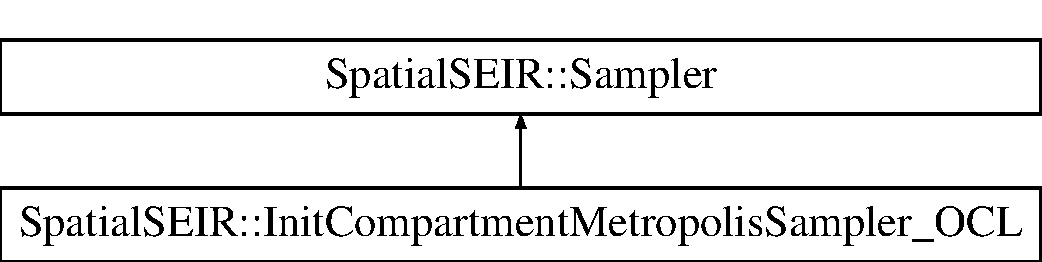
\includegraphics[height=2.000000cm]{classSpatialSEIR_1_1InitCompartmentMetropolisSampler__OCL}
\end{center}
\end{figure}
\subsection*{Public Member Functions}
\begin{DoxyCompactItemize}
\item 
\hyperlink{classSpatialSEIR_1_1InitCompartmentMetropolisSampler__OCL_ae77e54902afe126d8c6aeb84a8b36ddc}{Init\-Compartment\-Metropolis\-Sampler\-\_\-\-O\-C\-L} (\hyperlink{classSpatialSEIR_1_1ModelContext}{Model\-Context} $\ast$\hyperlink{classSpatialSEIR_1_1InitCompartmentMetropolisSampler__OCL_af79702dd1769bd3b988afdd33d975830}{context}, \hyperlink{classSpatialSEIR_1_1InitCompartmentFullConditional}{Init\-Compartment\-Full\-Conditional} $\ast$\hyperlink{classSpatialSEIR_1_1InitCompartmentMetropolisSampler__OCL_a1081812ec3f70109ed016877c7f44db2}{init\-Compartment\-F\-C}, int $\ast$\hyperlink{classSpatialSEIR_1_1InitCompartmentMetropolisSampler__OCL_a1f3d1244aa54a5d0530e8d31e36108c8}{init\-Compartment\-Data})
\item 
void \hyperlink{classSpatialSEIR_1_1InitCompartmentMetropolisSampler__OCL_aeb2831c79b43252f3a2a48f405cfccbe}{draw\-Sample} ()
\item 
int \hyperlink{classSpatialSEIR_1_1InitCompartmentMetropolisSampler__OCL_a932637bc74c6f2f5fc251dd4a81131ae}{get\-Sampler\-Type} ()
\item 
\hyperlink{classSpatialSEIR_1_1InitCompartmentMetropolisSampler__OCL_a8da634a1bf2df13dc4fcc3b9a9c1ccab}{$\sim$\-Init\-Compartment\-Metropolis\-Sampler\-\_\-\-O\-C\-L} ()
\end{DoxyCompactItemize}
\subsection*{Public Attributes}
\begin{DoxyCompactItemize}
\item 
\hyperlink{classSpatialSEIR_1_1ModelContext}{Model\-Context} $\ast$$\ast$ \hyperlink{classSpatialSEIR_1_1InitCompartmentMetropolisSampler__OCL_af79702dd1769bd3b988afdd33d975830}{context}
\item 
\hyperlink{classSpatialSEIR_1_1InitCompartmentFullConditional}{Init\-Compartment\-Full\-Conditional} $\ast$$\ast$ \hyperlink{classSpatialSEIR_1_1InitCompartmentMetropolisSampler__OCL_a1081812ec3f70109ed016877c7f44db2}{init\-Compartment\-F\-C}
\item 
int $\ast$$\ast$ \hyperlink{classSpatialSEIR_1_1InitCompartmentMetropolisSampler__OCL_a1f3d1244aa54a5d0530e8d31e36108c8}{init\-Compartment\-Data}
\end{DoxyCompactItemize}


\subsection{Detailed Description}
The \hyperlink{classSpatialSEIR_1_1InitCompartmentMetropolisSampler__OCL}{Init\-Compartment\-Metropolis\-Sampler\-\_\-\-O\-C\-L} functions identically to the \hyperlink{classSpatialSEIR_1_1CompartmentMetropolisSampler__OCL}{Compartment\-Metropolis\-Sampler\-\_\-\-O\-C\-L} class, but for the vector of initial values of each \hyperlink{classSpatialSEIR_1_1CompartmentalModelMatrix}{Compartmental\-Model\-Matrix}. This class makes use of the Open\-C\-L functionality of libspatial\-S\-E\-I\-R 

\subsection{Constructor \& Destructor Documentation}
\hypertarget{classSpatialSEIR_1_1InitCompartmentMetropolisSampler__OCL_ae77e54902afe126d8c6aeb84a8b36ddc}{\index{Spatial\-S\-E\-I\-R\-::\-Init\-Compartment\-Metropolis\-Sampler\-\_\-\-O\-C\-L@{Spatial\-S\-E\-I\-R\-::\-Init\-Compartment\-Metropolis\-Sampler\-\_\-\-O\-C\-L}!Init\-Compartment\-Metropolis\-Sampler\-\_\-\-O\-C\-L@{Init\-Compartment\-Metropolis\-Sampler\-\_\-\-O\-C\-L}}
\index{Init\-Compartment\-Metropolis\-Sampler\-\_\-\-O\-C\-L@{Init\-Compartment\-Metropolis\-Sampler\-\_\-\-O\-C\-L}!SpatialSEIR::InitCompartmentMetropolisSampler_OCL@{Spatial\-S\-E\-I\-R\-::\-Init\-Compartment\-Metropolis\-Sampler\-\_\-\-O\-C\-L}}
\subsubsection[{Init\-Compartment\-Metropolis\-Sampler\-\_\-\-O\-C\-L}]{\setlength{\rightskip}{0pt plus 5cm}Spatial\-S\-E\-I\-R\-::\-Init\-Compartment\-Metropolis\-Sampler\-\_\-\-O\-C\-L\-::\-Init\-Compartment\-Metropolis\-Sampler\-\_\-\-O\-C\-L (
\begin{DoxyParamCaption}
\item[{{\bf Model\-Context} $\ast$}]{context, }
\item[{{\bf Init\-Compartment\-Full\-Conditional} $\ast$}]{init\-Compartment\-F\-C, }
\item[{int $\ast$}]{init\-Compartment\-Data}
\end{DoxyParamCaption}
)}}\label{classSpatialSEIR_1_1InitCompartmentMetropolisSampler__OCL_ae77e54902afe126d8c6aeb84a8b36ddc}
\hypertarget{classSpatialSEIR_1_1InitCompartmentMetropolisSampler__OCL_a8da634a1bf2df13dc4fcc3b9a9c1ccab}{\index{Spatial\-S\-E\-I\-R\-::\-Init\-Compartment\-Metropolis\-Sampler\-\_\-\-O\-C\-L@{Spatial\-S\-E\-I\-R\-::\-Init\-Compartment\-Metropolis\-Sampler\-\_\-\-O\-C\-L}!$\sim$\-Init\-Compartment\-Metropolis\-Sampler\-\_\-\-O\-C\-L@{$\sim$\-Init\-Compartment\-Metropolis\-Sampler\-\_\-\-O\-C\-L}}
\index{$\sim$\-Init\-Compartment\-Metropolis\-Sampler\-\_\-\-O\-C\-L@{$\sim$\-Init\-Compartment\-Metropolis\-Sampler\-\_\-\-O\-C\-L}!SpatialSEIR::InitCompartmentMetropolisSampler_OCL@{Spatial\-S\-E\-I\-R\-::\-Init\-Compartment\-Metropolis\-Sampler\-\_\-\-O\-C\-L}}
\subsubsection[{$\sim$\-Init\-Compartment\-Metropolis\-Sampler\-\_\-\-O\-C\-L}]{\setlength{\rightskip}{0pt plus 5cm}Spatial\-S\-E\-I\-R\-::\-Init\-Compartment\-Metropolis\-Sampler\-\_\-\-O\-C\-L\-::$\sim$\-Init\-Compartment\-Metropolis\-Sampler\-\_\-\-O\-C\-L (
\begin{DoxyParamCaption}
{}
\end{DoxyParamCaption}
)}}\label{classSpatialSEIR_1_1InitCompartmentMetropolisSampler__OCL_a8da634a1bf2df13dc4fcc3b9a9c1ccab}


\subsection{Member Function Documentation}
\hypertarget{classSpatialSEIR_1_1InitCompartmentMetropolisSampler__OCL_aeb2831c79b43252f3a2a48f405cfccbe}{\index{Spatial\-S\-E\-I\-R\-::\-Init\-Compartment\-Metropolis\-Sampler\-\_\-\-O\-C\-L@{Spatial\-S\-E\-I\-R\-::\-Init\-Compartment\-Metropolis\-Sampler\-\_\-\-O\-C\-L}!draw\-Sample@{draw\-Sample}}
\index{draw\-Sample@{draw\-Sample}!SpatialSEIR::InitCompartmentMetropolisSampler_OCL@{Spatial\-S\-E\-I\-R\-::\-Init\-Compartment\-Metropolis\-Sampler\-\_\-\-O\-C\-L}}
\subsubsection[{draw\-Sample}]{\setlength{\rightskip}{0pt plus 5cm}void Spatial\-S\-E\-I\-R\-::\-Init\-Compartment\-Metropolis\-Sampler\-\_\-\-O\-C\-L\-::draw\-Sample (
\begin{DoxyParamCaption}
{}
\end{DoxyParamCaption}
)\hspace{0.3cm}{\ttfamily [virtual]}}}\label{classSpatialSEIR_1_1InitCompartmentMetropolisSampler__OCL_aeb2831c79b43252f3a2a48f405cfccbe}


Implements \hyperlink{classSpatialSEIR_1_1Sampler_aa07a42b26cb62249c20c58e855a08657}{Spatial\-S\-E\-I\-R\-::\-Sampler}.

\hypertarget{classSpatialSEIR_1_1InitCompartmentMetropolisSampler__OCL_a932637bc74c6f2f5fc251dd4a81131ae}{\index{Spatial\-S\-E\-I\-R\-::\-Init\-Compartment\-Metropolis\-Sampler\-\_\-\-O\-C\-L@{Spatial\-S\-E\-I\-R\-::\-Init\-Compartment\-Metropolis\-Sampler\-\_\-\-O\-C\-L}!get\-Sampler\-Type@{get\-Sampler\-Type}}
\index{get\-Sampler\-Type@{get\-Sampler\-Type}!SpatialSEIR::InitCompartmentMetropolisSampler_OCL@{Spatial\-S\-E\-I\-R\-::\-Init\-Compartment\-Metropolis\-Sampler\-\_\-\-O\-C\-L}}
\subsubsection[{get\-Sampler\-Type}]{\setlength{\rightskip}{0pt plus 5cm}int Spatial\-S\-E\-I\-R\-::\-Init\-Compartment\-Metropolis\-Sampler\-\_\-\-O\-C\-L\-::get\-Sampler\-Type (
\begin{DoxyParamCaption}
{}
\end{DoxyParamCaption}
)\hspace{0.3cm}{\ttfamily [virtual]}}}\label{classSpatialSEIR_1_1InitCompartmentMetropolisSampler__OCL_a932637bc74c6f2f5fc251dd4a81131ae}


Implements \hyperlink{classSpatialSEIR_1_1Sampler_aaa79310ad809e6aeb25479849f322dda}{Spatial\-S\-E\-I\-R\-::\-Sampler}.



\subsection{Member Data Documentation}
\hypertarget{classSpatialSEIR_1_1InitCompartmentMetropolisSampler__OCL_af79702dd1769bd3b988afdd33d975830}{\index{Spatial\-S\-E\-I\-R\-::\-Init\-Compartment\-Metropolis\-Sampler\-\_\-\-O\-C\-L@{Spatial\-S\-E\-I\-R\-::\-Init\-Compartment\-Metropolis\-Sampler\-\_\-\-O\-C\-L}!context@{context}}
\index{context@{context}!SpatialSEIR::InitCompartmentMetropolisSampler_OCL@{Spatial\-S\-E\-I\-R\-::\-Init\-Compartment\-Metropolis\-Sampler\-\_\-\-O\-C\-L}}
\subsubsection[{context}]{\setlength{\rightskip}{0pt plus 5cm}{\bf Model\-Context}$\ast$$\ast$ Spatial\-S\-E\-I\-R\-::\-Init\-Compartment\-Metropolis\-Sampler\-\_\-\-O\-C\-L\-::context}}\label{classSpatialSEIR_1_1InitCompartmentMetropolisSampler__OCL_af79702dd1769bd3b988afdd33d975830}
\hypertarget{classSpatialSEIR_1_1InitCompartmentMetropolisSampler__OCL_a1f3d1244aa54a5d0530e8d31e36108c8}{\index{Spatial\-S\-E\-I\-R\-::\-Init\-Compartment\-Metropolis\-Sampler\-\_\-\-O\-C\-L@{Spatial\-S\-E\-I\-R\-::\-Init\-Compartment\-Metropolis\-Sampler\-\_\-\-O\-C\-L}!init\-Compartment\-Data@{init\-Compartment\-Data}}
\index{init\-Compartment\-Data@{init\-Compartment\-Data}!SpatialSEIR::InitCompartmentMetropolisSampler_OCL@{Spatial\-S\-E\-I\-R\-::\-Init\-Compartment\-Metropolis\-Sampler\-\_\-\-O\-C\-L}}
\subsubsection[{init\-Compartment\-Data}]{\setlength{\rightskip}{0pt plus 5cm}int$\ast$$\ast$ Spatial\-S\-E\-I\-R\-::\-Init\-Compartment\-Metropolis\-Sampler\-\_\-\-O\-C\-L\-::init\-Compartment\-Data}}\label{classSpatialSEIR_1_1InitCompartmentMetropolisSampler__OCL_a1f3d1244aa54a5d0530e8d31e36108c8}
\hypertarget{classSpatialSEIR_1_1InitCompartmentMetropolisSampler__OCL_a1081812ec3f70109ed016877c7f44db2}{\index{Spatial\-S\-E\-I\-R\-::\-Init\-Compartment\-Metropolis\-Sampler\-\_\-\-O\-C\-L@{Spatial\-S\-E\-I\-R\-::\-Init\-Compartment\-Metropolis\-Sampler\-\_\-\-O\-C\-L}!init\-Compartment\-F\-C@{init\-Compartment\-F\-C}}
\index{init\-Compartment\-F\-C@{init\-Compartment\-F\-C}!SpatialSEIR::InitCompartmentMetropolisSampler_OCL@{Spatial\-S\-E\-I\-R\-::\-Init\-Compartment\-Metropolis\-Sampler\-\_\-\-O\-C\-L}}
\subsubsection[{init\-Compartment\-F\-C}]{\setlength{\rightskip}{0pt plus 5cm}{\bf Init\-Compartment\-Full\-Conditional}$\ast$$\ast$ Spatial\-S\-E\-I\-R\-::\-Init\-Compartment\-Metropolis\-Sampler\-\_\-\-O\-C\-L\-::init\-Compartment\-F\-C}}\label{classSpatialSEIR_1_1InitCompartmentMetropolisSampler__OCL_a1081812ec3f70109ed016877c7f44db2}


The documentation for this class was generated from the following file\-:\begin{DoxyCompactItemize}
\item 
lib\-Spatial\-S\-E\-I\-R/include/\hyperlink{LSS__Samplers_8hpp}{L\-S\-S\-\_\-\-Samplers.\-hpp}\end{DoxyCompactItemize}

\hypertarget{classSpatialSEIR_1_1InitData}{\section{Spatial\-S\-E\-I\-R\-:\-:Init\-Data Class Reference}
\label{classSpatialSEIR_1_1InitData}\index{Spatial\-S\-E\-I\-R\-::\-Init\-Data@{Spatial\-S\-E\-I\-R\-::\-Init\-Data}}
}


Simple class containing the starting compartment sizes.  




{\ttfamily \#include $<$L\-S\-S\-\_\-\-Full\-Conditional.\-hpp$>$}

\subsection*{Public Member Functions}
\begin{DoxyCompactItemize}
\item 
\hyperlink{classSpatialSEIR_1_1InitData_afc3aab95825d04fdc7e8eac643ba815e}{Init\-Data} (int $\ast$\-\_\-\-S0, int $\ast$\-\_\-\-E0, int $\ast$\-\_\-\-I0, int $\ast$\-\_\-\-R0, int $\ast$n\-Loc)
\item 
\hyperlink{classSpatialSEIR_1_1InitData_a7d85d0f9287cb0dc484b85fad0a1df94}{Init\-Data} ()
\item 
void \hyperlink{classSpatialSEIR_1_1InitData_abfcf6cd81728b081dfe1b9ff1137b42b}{populate} (int $\ast$\-\_\-\-S0, int $\ast$\-\_\-\-E0, int $\ast$\-\_\-\-I0, int $\ast$\-\_\-\-R0, int $\ast$n\-Loc)
\item 
\hyperlink{classSpatialSEIR_1_1InitData_a9868dfc71831843b28c1480f79fffdc3}{$\sim$\-Init\-Data} ()
\end{DoxyCompactItemize}
\subsection*{Public Attributes}
\begin{DoxyCompactItemize}
\item 
int $\ast$ \hyperlink{classSpatialSEIR_1_1InitData_a349ab7c6e53a1777cd119e59a995c781}{S0}
\item 
int $\ast$ \hyperlink{classSpatialSEIR_1_1InitData_a17086ef1f134d23265360450ed24e77c}{E0}
\item 
int $\ast$ \hyperlink{classSpatialSEIR_1_1InitData_a393dd2e968876861412439caf2e3c05b}{I0}
\item 
int $\ast$ \hyperlink{classSpatialSEIR_1_1InitData_a45a1241af922fb151c91cb669cbdf106}{R0}
\item 
int $\ast$ \hyperlink{classSpatialSEIR_1_1InitData_aa9bc45e52403b6a9779acf3ab51f451b}{num\-Locations}
\end{DoxyCompactItemize}


\subsection{Detailed Description}
Simple class containing the starting compartment sizes. 

\subsection{Constructor \& Destructor Documentation}
\hypertarget{classSpatialSEIR_1_1InitData_afc3aab95825d04fdc7e8eac643ba815e}{\index{Spatial\-S\-E\-I\-R\-::\-Init\-Data@{Spatial\-S\-E\-I\-R\-::\-Init\-Data}!Init\-Data@{Init\-Data}}
\index{Init\-Data@{Init\-Data}!SpatialSEIR::InitData@{Spatial\-S\-E\-I\-R\-::\-Init\-Data}}
\subsubsection[{Init\-Data}]{\setlength{\rightskip}{0pt plus 5cm}Spatial\-S\-E\-I\-R\-::\-Init\-Data\-::\-Init\-Data (
\begin{DoxyParamCaption}
\item[{int $\ast$}]{\-\_\-\-S0, }
\item[{int $\ast$}]{\-\_\-\-E0, }
\item[{int $\ast$}]{\-\_\-\-I0, }
\item[{int $\ast$}]{\-\_\-\-R0, }
\item[{int $\ast$}]{n\-Loc}
\end{DoxyParamCaption}
)}}\label{classSpatialSEIR_1_1InitData_afc3aab95825d04fdc7e8eac643ba815e}
\hypertarget{classSpatialSEIR_1_1InitData_a7d85d0f9287cb0dc484b85fad0a1df94}{\index{Spatial\-S\-E\-I\-R\-::\-Init\-Data@{Spatial\-S\-E\-I\-R\-::\-Init\-Data}!Init\-Data@{Init\-Data}}
\index{Init\-Data@{Init\-Data}!SpatialSEIR::InitData@{Spatial\-S\-E\-I\-R\-::\-Init\-Data}}
\subsubsection[{Init\-Data}]{\setlength{\rightskip}{0pt plus 5cm}Spatial\-S\-E\-I\-R\-::\-Init\-Data\-::\-Init\-Data (
\begin{DoxyParamCaption}
{}
\end{DoxyParamCaption}
)}}\label{classSpatialSEIR_1_1InitData_a7d85d0f9287cb0dc484b85fad0a1df94}
\hypertarget{classSpatialSEIR_1_1InitData_a9868dfc71831843b28c1480f79fffdc3}{\index{Spatial\-S\-E\-I\-R\-::\-Init\-Data@{Spatial\-S\-E\-I\-R\-::\-Init\-Data}!$\sim$\-Init\-Data@{$\sim$\-Init\-Data}}
\index{$\sim$\-Init\-Data@{$\sim$\-Init\-Data}!SpatialSEIR::InitData@{Spatial\-S\-E\-I\-R\-::\-Init\-Data}}
\subsubsection[{$\sim$\-Init\-Data}]{\setlength{\rightskip}{0pt plus 5cm}Spatial\-S\-E\-I\-R\-::\-Init\-Data\-::$\sim$\-Init\-Data (
\begin{DoxyParamCaption}
{}
\end{DoxyParamCaption}
)}}\label{classSpatialSEIR_1_1InitData_a9868dfc71831843b28c1480f79fffdc3}


\subsection{Member Function Documentation}
\hypertarget{classSpatialSEIR_1_1InitData_abfcf6cd81728b081dfe1b9ff1137b42b}{\index{Spatial\-S\-E\-I\-R\-::\-Init\-Data@{Spatial\-S\-E\-I\-R\-::\-Init\-Data}!populate@{populate}}
\index{populate@{populate}!SpatialSEIR::InitData@{Spatial\-S\-E\-I\-R\-::\-Init\-Data}}
\subsubsection[{populate}]{\setlength{\rightskip}{0pt plus 5cm}void Spatial\-S\-E\-I\-R\-::\-Init\-Data\-::populate (
\begin{DoxyParamCaption}
\item[{int $\ast$}]{\-\_\-\-S0, }
\item[{int $\ast$}]{\-\_\-\-E0, }
\item[{int $\ast$}]{\-\_\-\-I0, }
\item[{int $\ast$}]{\-\_\-\-R0, }
\item[{int $\ast$}]{n\-Loc}
\end{DoxyParamCaption}
)}}\label{classSpatialSEIR_1_1InitData_abfcf6cd81728b081dfe1b9ff1137b42b}


\subsection{Member Data Documentation}
\hypertarget{classSpatialSEIR_1_1InitData_a17086ef1f134d23265360450ed24e77c}{\index{Spatial\-S\-E\-I\-R\-::\-Init\-Data@{Spatial\-S\-E\-I\-R\-::\-Init\-Data}!E0@{E0}}
\index{E0@{E0}!SpatialSEIR::InitData@{Spatial\-S\-E\-I\-R\-::\-Init\-Data}}
\subsubsection[{E0}]{\setlength{\rightskip}{0pt plus 5cm}int$\ast$ Spatial\-S\-E\-I\-R\-::\-Init\-Data\-::\-E0}}\label{classSpatialSEIR_1_1InitData_a17086ef1f134d23265360450ed24e77c}
\hypertarget{classSpatialSEIR_1_1InitData_a393dd2e968876861412439caf2e3c05b}{\index{Spatial\-S\-E\-I\-R\-::\-Init\-Data@{Spatial\-S\-E\-I\-R\-::\-Init\-Data}!I0@{I0}}
\index{I0@{I0}!SpatialSEIR::InitData@{Spatial\-S\-E\-I\-R\-::\-Init\-Data}}
\subsubsection[{I0}]{\setlength{\rightskip}{0pt plus 5cm}int$\ast$ Spatial\-S\-E\-I\-R\-::\-Init\-Data\-::\-I0}}\label{classSpatialSEIR_1_1InitData_a393dd2e968876861412439caf2e3c05b}
\hypertarget{classSpatialSEIR_1_1InitData_aa9bc45e52403b6a9779acf3ab51f451b}{\index{Spatial\-S\-E\-I\-R\-::\-Init\-Data@{Spatial\-S\-E\-I\-R\-::\-Init\-Data}!num\-Locations@{num\-Locations}}
\index{num\-Locations@{num\-Locations}!SpatialSEIR::InitData@{Spatial\-S\-E\-I\-R\-::\-Init\-Data}}
\subsubsection[{num\-Locations}]{\setlength{\rightskip}{0pt plus 5cm}int$\ast$ Spatial\-S\-E\-I\-R\-::\-Init\-Data\-::num\-Locations}}\label{classSpatialSEIR_1_1InitData_aa9bc45e52403b6a9779acf3ab51f451b}
\hypertarget{classSpatialSEIR_1_1InitData_a45a1241af922fb151c91cb669cbdf106}{\index{Spatial\-S\-E\-I\-R\-::\-Init\-Data@{Spatial\-S\-E\-I\-R\-::\-Init\-Data}!R0@{R0}}
\index{R0@{R0}!SpatialSEIR::InitData@{Spatial\-S\-E\-I\-R\-::\-Init\-Data}}
\subsubsection[{R0}]{\setlength{\rightskip}{0pt plus 5cm}int$\ast$ Spatial\-S\-E\-I\-R\-::\-Init\-Data\-::\-R0}}\label{classSpatialSEIR_1_1InitData_a45a1241af922fb151c91cb669cbdf106}
\hypertarget{classSpatialSEIR_1_1InitData_a349ab7c6e53a1777cd119e59a995c781}{\index{Spatial\-S\-E\-I\-R\-::\-Init\-Data@{Spatial\-S\-E\-I\-R\-::\-Init\-Data}!S0@{S0}}
\index{S0@{S0}!SpatialSEIR::InitData@{Spatial\-S\-E\-I\-R\-::\-Init\-Data}}
\subsubsection[{S0}]{\setlength{\rightskip}{0pt plus 5cm}int$\ast$ Spatial\-S\-E\-I\-R\-::\-Init\-Data\-::\-S0}}\label{classSpatialSEIR_1_1InitData_a349ab7c6e53a1777cd119e59a995c781}


The documentation for this class was generated from the following files\-:\begin{DoxyCompactItemize}
\item 
lib\-Spatial\-S\-E\-I\-R/include/\-Full\-Conditionals/\hyperlink{LSS__FullConditional_8hpp}{L\-S\-S\-\_\-\-Full\-Conditional.\-hpp}\item 
lib\-Spatial\-S\-E\-I\-R/src/\-Full\-Conditionals/\hyperlink{FullConditional_8cpp}{Full\-Conditional.\-cpp}\end{DoxyCompactItemize}

\hypertarget{classSpatialSEIR_1_1IOProvider}{\section{Spatial\-S\-E\-I\-R\-:\-:I\-O\-Provider Class Reference}
\label{classSpatialSEIR_1_1IOProvider}\index{Spatial\-S\-E\-I\-R\-::\-I\-O\-Provider@{Spatial\-S\-E\-I\-R\-::\-I\-O\-Provider}}
}


{\ttfamily \#include $<$I\-O\-Provider.\-hpp$>$}

\subsection*{Public Member Functions}
\begin{DoxyCompactItemize}
\item 
\hyperlink{classSpatialSEIR_1_1IOProvider_ae89a408ae26e4a8b0dc6ed7279dcb7db}{I\-O\-Provider} ()
\item 
\hyperlink{classSpatialSEIR_1_1IOProvider_a933b502eeaa05b44bf1bef52c042659c}{I\-O\-Provider} (\hyperlink{classSpatialSEIR_1_1ModelContext}{Model\-Context} $\ast$\hyperlink{classSpatialSEIR_1_1IOProvider_add6cc02df595bc12b3ac76ce148cc3dc}{context}, std\-::string $\ast$\hyperlink{classSpatialSEIR_1_1IOProvider_a744600dd48a3b8a0f6d65dda5f160bda}{out\-File\-Path}, int $\ast$\hyperlink{classSpatialSEIR_1_1IOProvider_a756afb68ee349d9715566fa9fdc4d37e}{iteration\-Stride})
\item 
int \hyperlink{classSpatialSEIR_1_1IOProvider_a3472f7209ca2a3759a47e619f7832432}{populate} (\hyperlink{classSpatialSEIR_1_1ModelContext}{Model\-Context} $\ast$\hyperlink{classSpatialSEIR_1_1IOProvider_add6cc02df595bc12b3ac76ce148cc3dc}{context}, std\-::string $\ast$\hyperlink{classSpatialSEIR_1_1IOProvider_a744600dd48a3b8a0f6d65dda5f160bda}{out\-File\-Path}, int $\ast$\hyperlink{classSpatialSEIR_1_1IOProvider_a756afb68ee349d9715566fa9fdc4d37e}{iteration\-Stride})
\item 
void \hyperlink{classSpatialSEIR_1_1IOProvider_aa7568ce7698cad0aea3c429f1833f0bb}{set\-Trace} (int location\-Index)
\item 
void \hyperlink{classSpatialSEIR_1_1IOProvider_aa61e367e84b6f8a5377f7255877213e3}{set\-Trace} (int location\-Index, int time\-Index)
\item 
int \hyperlink{classSpatialSEIR_1_1IOProvider_a4951df99453c659fa25503781932373c}{close} ()
\item 
int \hyperlink{classSpatialSEIR_1_1IOProvider_afa6b6c8fd164717fd7ccfd1d08c4dca4}{file\-Init} ()
\item 
int \hyperlink{classSpatialSEIR_1_1IOProvider_a5ab95092c0c23757c54440ef1b78ad53}{cat\-Iter} (int iteration)
\item 
\hyperlink{classSpatialSEIR_1_1IOProvider_a1706d3ce051c5d8454fd8cf3b4c51d07}{$\sim$\-I\-O\-Provider} ()
\end{DoxyCompactItemize}
\subsection*{Public Attributes}
\begin{DoxyCompactItemize}
\item 
\hyperlink{classSpatialSEIR_1_1ModelContext}{Model\-Context} $\ast$$\ast$ \hyperlink{classSpatialSEIR_1_1IOProvider_add6cc02df595bc12b3ac76ce148cc3dc}{context}
\item 
int $\ast$ \hyperlink{classSpatialSEIR_1_1IOProvider_a756afb68ee349d9715566fa9fdc4d37e}{iteration\-Stride}
\item 
bool $\ast$ \hyperlink{classSpatialSEIR_1_1IOProvider_ac482c0b2eccc9c587a08ae61f588e23e}{is\-Open}
\item 
time\-\_\-t $\ast$ \hyperlink{classSpatialSEIR_1_1IOProvider_acab89531190c3433ea0fe1bc3f14aa0f}{timer}
\item 
time\-\_\-t $\ast$ \hyperlink{classSpatialSEIR_1_1IOProvider_a4900b2f77db4845e2db1e5511b1f513b}{start\-Time}
\item 
std\-::vector$<$ \hyperlink{structSpatialSEIR_1_1TimeLocationTrace}{Time\-Location\-Trace} $\ast$ $>$ $\ast$ \hyperlink{classSpatialSEIR_1_1IOProvider_ad1fa227b00c230cc9549e682c17d5c1c}{time\-Location\-Traces}
\item 
std\-::vector$<$ \hyperlink{structSpatialSEIR_1_1LocationTrace}{Location\-Trace} $\ast$ $>$ $\ast$ \hyperlink{classSpatialSEIR_1_1IOProvider_a3dcb1c064746cd7e9fd6e15c1b55540d}{location\-Traces}
\item 
std\-::ofstream $\ast$ \hyperlink{classSpatialSEIR_1_1IOProvider_a7ce442ee5f7eda58ff86e68d3df07edc}{out\-File\-Stream}
\item 
std\-::string $\ast$ \hyperlink{classSpatialSEIR_1_1IOProvider_a744600dd48a3b8a0f6d65dda5f160bda}{out\-File\-Path}
\end{DoxyCompactItemize}


\subsection{Detailed Description}
The \hyperlink{classSpatialSEIR_1_1IOProvider}{I\-O\-Provider} class handles file output operations. You might expect given the name that it handled file input operations as well, but you would be mistaken. Mainly it writes M\-C\-M\-C sample output. The user shouldn't really need to interact with it, as \hyperlink{classSpatialSEIR_1_1ModelContext}{Model\-Context} handles the basics. 

\subsection{Constructor \& Destructor Documentation}
\hypertarget{classSpatialSEIR_1_1IOProvider_ae89a408ae26e4a8b0dc6ed7279dcb7db}{\index{Spatial\-S\-E\-I\-R\-::\-I\-O\-Provider@{Spatial\-S\-E\-I\-R\-::\-I\-O\-Provider}!I\-O\-Provider@{I\-O\-Provider}}
\index{I\-O\-Provider@{I\-O\-Provider}!SpatialSEIR::IOProvider@{Spatial\-S\-E\-I\-R\-::\-I\-O\-Provider}}
\subsubsection[{I\-O\-Provider}]{\setlength{\rightskip}{0pt plus 5cm}Spatial\-S\-E\-I\-R\-::\-I\-O\-Provider\-::\-I\-O\-Provider (
\begin{DoxyParamCaption}
{}
\end{DoxyParamCaption}
)}}\label{classSpatialSEIR_1_1IOProvider_ae89a408ae26e4a8b0dc6ed7279dcb7db}
\hypertarget{classSpatialSEIR_1_1IOProvider_a933b502eeaa05b44bf1bef52c042659c}{\index{Spatial\-S\-E\-I\-R\-::\-I\-O\-Provider@{Spatial\-S\-E\-I\-R\-::\-I\-O\-Provider}!I\-O\-Provider@{I\-O\-Provider}}
\index{I\-O\-Provider@{I\-O\-Provider}!SpatialSEIR::IOProvider@{Spatial\-S\-E\-I\-R\-::\-I\-O\-Provider}}
\subsubsection[{I\-O\-Provider}]{\setlength{\rightskip}{0pt plus 5cm}Spatial\-S\-E\-I\-R\-::\-I\-O\-Provider\-::\-I\-O\-Provider (
\begin{DoxyParamCaption}
\item[{{\bf Model\-Context} $\ast$}]{context, }
\item[{std\-::string $\ast$}]{out\-File\-Path, }
\item[{int $\ast$}]{iteration\-Stride}
\end{DoxyParamCaption}
)}}\label{classSpatialSEIR_1_1IOProvider_a933b502eeaa05b44bf1bef52c042659c}
\hypertarget{classSpatialSEIR_1_1IOProvider_a1706d3ce051c5d8454fd8cf3b4c51d07}{\index{Spatial\-S\-E\-I\-R\-::\-I\-O\-Provider@{Spatial\-S\-E\-I\-R\-::\-I\-O\-Provider}!$\sim$\-I\-O\-Provider@{$\sim$\-I\-O\-Provider}}
\index{$\sim$\-I\-O\-Provider@{$\sim$\-I\-O\-Provider}!SpatialSEIR::IOProvider@{Spatial\-S\-E\-I\-R\-::\-I\-O\-Provider}}
\subsubsection[{$\sim$\-I\-O\-Provider}]{\setlength{\rightskip}{0pt plus 5cm}Spatial\-S\-E\-I\-R\-::\-I\-O\-Provider\-::$\sim$\-I\-O\-Provider (
\begin{DoxyParamCaption}
{}
\end{DoxyParamCaption}
)}}\label{classSpatialSEIR_1_1IOProvider_a1706d3ce051c5d8454fd8cf3b4c51d07}


\subsection{Member Function Documentation}
\hypertarget{classSpatialSEIR_1_1IOProvider_a5ab95092c0c23757c54440ef1b78ad53}{\index{Spatial\-S\-E\-I\-R\-::\-I\-O\-Provider@{Spatial\-S\-E\-I\-R\-::\-I\-O\-Provider}!cat\-Iter@{cat\-Iter}}
\index{cat\-Iter@{cat\-Iter}!SpatialSEIR::IOProvider@{Spatial\-S\-E\-I\-R\-::\-I\-O\-Provider}}
\subsubsection[{cat\-Iter}]{\setlength{\rightskip}{0pt plus 5cm}int Spatial\-S\-E\-I\-R\-::\-I\-O\-Provider\-::cat\-Iter (
\begin{DoxyParamCaption}
\item[{int}]{iteration}
\end{DoxyParamCaption}
)}}\label{classSpatialSEIR_1_1IOProvider_a5ab95092c0c23757c54440ef1b78ad53}
\hypertarget{classSpatialSEIR_1_1IOProvider_a4951df99453c659fa25503781932373c}{\index{Spatial\-S\-E\-I\-R\-::\-I\-O\-Provider@{Spatial\-S\-E\-I\-R\-::\-I\-O\-Provider}!close@{close}}
\index{close@{close}!SpatialSEIR::IOProvider@{Spatial\-S\-E\-I\-R\-::\-I\-O\-Provider}}
\subsubsection[{close}]{\setlength{\rightskip}{0pt plus 5cm}int Spatial\-S\-E\-I\-R\-::\-I\-O\-Provider\-::close (
\begin{DoxyParamCaption}
{}
\end{DoxyParamCaption}
)}}\label{classSpatialSEIR_1_1IOProvider_a4951df99453c659fa25503781932373c}
\hypertarget{classSpatialSEIR_1_1IOProvider_afa6b6c8fd164717fd7ccfd1d08c4dca4}{\index{Spatial\-S\-E\-I\-R\-::\-I\-O\-Provider@{Spatial\-S\-E\-I\-R\-::\-I\-O\-Provider}!file\-Init@{file\-Init}}
\index{file\-Init@{file\-Init}!SpatialSEIR::IOProvider@{Spatial\-S\-E\-I\-R\-::\-I\-O\-Provider}}
\subsubsection[{file\-Init}]{\setlength{\rightskip}{0pt plus 5cm}int Spatial\-S\-E\-I\-R\-::\-I\-O\-Provider\-::file\-Init (
\begin{DoxyParamCaption}
{}
\end{DoxyParamCaption}
)}}\label{classSpatialSEIR_1_1IOProvider_afa6b6c8fd164717fd7ccfd1d08c4dca4}
\hypertarget{classSpatialSEIR_1_1IOProvider_a3472f7209ca2a3759a47e619f7832432}{\index{Spatial\-S\-E\-I\-R\-::\-I\-O\-Provider@{Spatial\-S\-E\-I\-R\-::\-I\-O\-Provider}!populate@{populate}}
\index{populate@{populate}!SpatialSEIR::IOProvider@{Spatial\-S\-E\-I\-R\-::\-I\-O\-Provider}}
\subsubsection[{populate}]{\setlength{\rightskip}{0pt plus 5cm}int Spatial\-S\-E\-I\-R\-::\-I\-O\-Provider\-::populate (
\begin{DoxyParamCaption}
\item[{{\bf Model\-Context} $\ast$}]{context, }
\item[{std\-::string $\ast$}]{out\-File\-Path, }
\item[{int $\ast$}]{iteration\-Stride}
\end{DoxyParamCaption}
)}}\label{classSpatialSEIR_1_1IOProvider_a3472f7209ca2a3759a47e619f7832432}
\hypertarget{classSpatialSEIR_1_1IOProvider_aa7568ce7698cad0aea3c429f1833f0bb}{\index{Spatial\-S\-E\-I\-R\-::\-I\-O\-Provider@{Spatial\-S\-E\-I\-R\-::\-I\-O\-Provider}!set\-Trace@{set\-Trace}}
\index{set\-Trace@{set\-Trace}!SpatialSEIR::IOProvider@{Spatial\-S\-E\-I\-R\-::\-I\-O\-Provider}}
\subsubsection[{set\-Trace}]{\setlength{\rightskip}{0pt plus 5cm}void Spatial\-S\-E\-I\-R\-::\-I\-O\-Provider\-::set\-Trace (
\begin{DoxyParamCaption}
\item[{int}]{location\-Index}
\end{DoxyParamCaption}
)}}\label{classSpatialSEIR_1_1IOProvider_aa7568ce7698cad0aea3c429f1833f0bb}
Keep track of compartment and transition probability information for location location\-Index \hypertarget{classSpatialSEIR_1_1IOProvider_aa61e367e84b6f8a5377f7255877213e3}{\index{Spatial\-S\-E\-I\-R\-::\-I\-O\-Provider@{Spatial\-S\-E\-I\-R\-::\-I\-O\-Provider}!set\-Trace@{set\-Trace}}
\index{set\-Trace@{set\-Trace}!SpatialSEIR::IOProvider@{Spatial\-S\-E\-I\-R\-::\-I\-O\-Provider}}
\subsubsection[{set\-Trace}]{\setlength{\rightskip}{0pt plus 5cm}void Spatial\-S\-E\-I\-R\-::\-I\-O\-Provider\-::set\-Trace (
\begin{DoxyParamCaption}
\item[{int}]{location\-Index, }
\item[{int}]{time\-Index}
\end{DoxyParamCaption}
)}}\label{classSpatialSEIR_1_1IOProvider_aa61e367e84b6f8a5377f7255877213e3}
Keep track of compartment and transition probability information for location location\-Index and time point time\-Index 

\subsection{Member Data Documentation}
\hypertarget{classSpatialSEIR_1_1IOProvider_add6cc02df595bc12b3ac76ce148cc3dc}{\index{Spatial\-S\-E\-I\-R\-::\-I\-O\-Provider@{Spatial\-S\-E\-I\-R\-::\-I\-O\-Provider}!context@{context}}
\index{context@{context}!SpatialSEIR::IOProvider@{Spatial\-S\-E\-I\-R\-::\-I\-O\-Provider}}
\subsubsection[{context}]{\setlength{\rightskip}{0pt plus 5cm}{\bf Model\-Context}$\ast$$\ast$ Spatial\-S\-E\-I\-R\-::\-I\-O\-Provider\-::context}}\label{classSpatialSEIR_1_1IOProvider_add6cc02df595bc12b3ac76ce148cc3dc}
\hypertarget{classSpatialSEIR_1_1IOProvider_ac482c0b2eccc9c587a08ae61f588e23e}{\index{Spatial\-S\-E\-I\-R\-::\-I\-O\-Provider@{Spatial\-S\-E\-I\-R\-::\-I\-O\-Provider}!is\-Open@{is\-Open}}
\index{is\-Open@{is\-Open}!SpatialSEIR::IOProvider@{Spatial\-S\-E\-I\-R\-::\-I\-O\-Provider}}
\subsubsection[{is\-Open}]{\setlength{\rightskip}{0pt plus 5cm}bool$\ast$ Spatial\-S\-E\-I\-R\-::\-I\-O\-Provider\-::is\-Open}}\label{classSpatialSEIR_1_1IOProvider_ac482c0b2eccc9c587a08ae61f588e23e}
\hypertarget{classSpatialSEIR_1_1IOProvider_a756afb68ee349d9715566fa9fdc4d37e}{\index{Spatial\-S\-E\-I\-R\-::\-I\-O\-Provider@{Spatial\-S\-E\-I\-R\-::\-I\-O\-Provider}!iteration\-Stride@{iteration\-Stride}}
\index{iteration\-Stride@{iteration\-Stride}!SpatialSEIR::IOProvider@{Spatial\-S\-E\-I\-R\-::\-I\-O\-Provider}}
\subsubsection[{iteration\-Stride}]{\setlength{\rightskip}{0pt plus 5cm}int$\ast$ Spatial\-S\-E\-I\-R\-::\-I\-O\-Provider\-::iteration\-Stride}}\label{classSpatialSEIR_1_1IOProvider_a756afb68ee349d9715566fa9fdc4d37e}
\hypertarget{classSpatialSEIR_1_1IOProvider_a3dcb1c064746cd7e9fd6e15c1b55540d}{\index{Spatial\-S\-E\-I\-R\-::\-I\-O\-Provider@{Spatial\-S\-E\-I\-R\-::\-I\-O\-Provider}!location\-Traces@{location\-Traces}}
\index{location\-Traces@{location\-Traces}!SpatialSEIR::IOProvider@{Spatial\-S\-E\-I\-R\-::\-I\-O\-Provider}}
\subsubsection[{location\-Traces}]{\setlength{\rightskip}{0pt plus 5cm}std\-::vector$<${\bf Location\-Trace}$\ast$$>$$\ast$ Spatial\-S\-E\-I\-R\-::\-I\-O\-Provider\-::location\-Traces}}\label{classSpatialSEIR_1_1IOProvider_a3dcb1c064746cd7e9fd6e15c1b55540d}
\hypertarget{classSpatialSEIR_1_1IOProvider_a744600dd48a3b8a0f6d65dda5f160bda}{\index{Spatial\-S\-E\-I\-R\-::\-I\-O\-Provider@{Spatial\-S\-E\-I\-R\-::\-I\-O\-Provider}!out\-File\-Path@{out\-File\-Path}}
\index{out\-File\-Path@{out\-File\-Path}!SpatialSEIR::IOProvider@{Spatial\-S\-E\-I\-R\-::\-I\-O\-Provider}}
\subsubsection[{out\-File\-Path}]{\setlength{\rightskip}{0pt plus 5cm}std\-::string$\ast$ Spatial\-S\-E\-I\-R\-::\-I\-O\-Provider\-::out\-File\-Path}}\label{classSpatialSEIR_1_1IOProvider_a744600dd48a3b8a0f6d65dda5f160bda}
\hypertarget{classSpatialSEIR_1_1IOProvider_a7ce442ee5f7eda58ff86e68d3df07edc}{\index{Spatial\-S\-E\-I\-R\-::\-I\-O\-Provider@{Spatial\-S\-E\-I\-R\-::\-I\-O\-Provider}!out\-File\-Stream@{out\-File\-Stream}}
\index{out\-File\-Stream@{out\-File\-Stream}!SpatialSEIR::IOProvider@{Spatial\-S\-E\-I\-R\-::\-I\-O\-Provider}}
\subsubsection[{out\-File\-Stream}]{\setlength{\rightskip}{0pt plus 5cm}std\-::ofstream$\ast$ Spatial\-S\-E\-I\-R\-::\-I\-O\-Provider\-::out\-File\-Stream}}\label{classSpatialSEIR_1_1IOProvider_a7ce442ee5f7eda58ff86e68d3df07edc}
\hypertarget{classSpatialSEIR_1_1IOProvider_a4900b2f77db4845e2db1e5511b1f513b}{\index{Spatial\-S\-E\-I\-R\-::\-I\-O\-Provider@{Spatial\-S\-E\-I\-R\-::\-I\-O\-Provider}!start\-Time@{start\-Time}}
\index{start\-Time@{start\-Time}!SpatialSEIR::IOProvider@{Spatial\-S\-E\-I\-R\-::\-I\-O\-Provider}}
\subsubsection[{start\-Time}]{\setlength{\rightskip}{0pt plus 5cm}time\-\_\-t$\ast$ Spatial\-S\-E\-I\-R\-::\-I\-O\-Provider\-::start\-Time}}\label{classSpatialSEIR_1_1IOProvider_a4900b2f77db4845e2db1e5511b1f513b}
\hypertarget{classSpatialSEIR_1_1IOProvider_ad1fa227b00c230cc9549e682c17d5c1c}{\index{Spatial\-S\-E\-I\-R\-::\-I\-O\-Provider@{Spatial\-S\-E\-I\-R\-::\-I\-O\-Provider}!time\-Location\-Traces@{time\-Location\-Traces}}
\index{time\-Location\-Traces@{time\-Location\-Traces}!SpatialSEIR::IOProvider@{Spatial\-S\-E\-I\-R\-::\-I\-O\-Provider}}
\subsubsection[{time\-Location\-Traces}]{\setlength{\rightskip}{0pt plus 5cm}std\-::vector$<${\bf Time\-Location\-Trace}$\ast$$>$$\ast$ Spatial\-S\-E\-I\-R\-::\-I\-O\-Provider\-::time\-Location\-Traces}}\label{classSpatialSEIR_1_1IOProvider_ad1fa227b00c230cc9549e682c17d5c1c}
\hypertarget{classSpatialSEIR_1_1IOProvider_acab89531190c3433ea0fe1bc3f14aa0f}{\index{Spatial\-S\-E\-I\-R\-::\-I\-O\-Provider@{Spatial\-S\-E\-I\-R\-::\-I\-O\-Provider}!timer@{timer}}
\index{timer@{timer}!SpatialSEIR::IOProvider@{Spatial\-S\-E\-I\-R\-::\-I\-O\-Provider}}
\subsubsection[{timer}]{\setlength{\rightskip}{0pt plus 5cm}time\-\_\-t$\ast$ Spatial\-S\-E\-I\-R\-::\-I\-O\-Provider\-::timer}}\label{classSpatialSEIR_1_1IOProvider_acab89531190c3433ea0fe1bc3f14aa0f}


The documentation for this class was generated from the following files\-:\begin{DoxyCompactItemize}
\item 
lib\-Spatial\-S\-E\-I\-R/include/\hyperlink{IOProvider_8hpp}{I\-O\-Provider.\-hpp}\item 
lib\-Spatial\-S\-E\-I\-R/src/\hyperlink{IOProvider_8cpp}{I\-O\-Provider.\-cpp}\end{DoxyCompactItemize}

\hypertarget{classSpatialSEIR_1_1IterationTask}{\section{Spatial\-S\-E\-I\-R\-:\-:Iteration\-Task Class Reference}
\label{classSpatialSEIR_1_1IterationTask}\index{Spatial\-S\-E\-I\-R\-::\-Iteration\-Task@{Spatial\-S\-E\-I\-R\-::\-Iteration\-Task}}
}


{\ttfamily \#include $<$L\-S\-S\-\_\-\-Iteration\-Tasks.\-hpp$>$}

Inheritance diagram for Spatial\-S\-E\-I\-R\-:\-:Iteration\-Task\-:\begin{figure}[H]
\begin{center}
\leavevmode
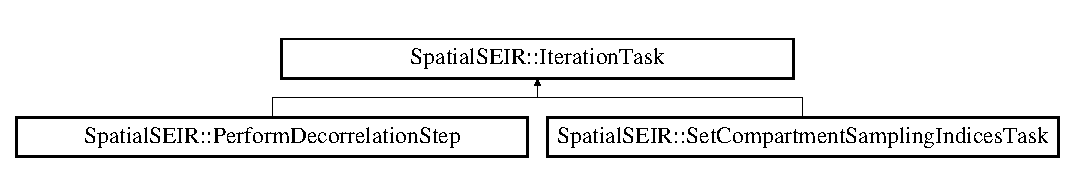
\includegraphics[height=1.248607cm]{classSpatialSEIR_1_1IterationTask}
\end{center}
\end{figure}
\subsection*{Public Member Functions}
\begin{DoxyCompactItemize}
\item 
virtual \hyperlink{classSpatialSEIR_1_1IterationTask_a042b6341e3fdf211ec7c6bf954b4258d}{$\sim$\-Iteration\-Task} ()
\item 
virtual void \hyperlink{classSpatialSEIR_1_1IterationTask_a68fcb08fe777ed506c97dc1ac5a0fb54}{execute\-Task} ()=0
\item 
virtual int \hyperlink{classSpatialSEIR_1_1IterationTask_aaba9c737c4564df6b44b843d7c781722}{get\-Task\-Type} ()=0
\end{DoxyCompactItemize}


\subsection{Detailed Description}
\hyperlink{classSpatialSEIR_1_1IterationTask}{Iteration\-Task} instances are bits of logical code that need to execute periodically during M\-C\-M\-C sampling and do not fall into the usual \hyperlink{classSpatialSEIR_1_1FullConditional}{Full\-Conditional} workflow. 

\subsection{Constructor \& Destructor Documentation}
\hypertarget{classSpatialSEIR_1_1IterationTask_a042b6341e3fdf211ec7c6bf954b4258d}{\index{Spatial\-S\-E\-I\-R\-::\-Iteration\-Task@{Spatial\-S\-E\-I\-R\-::\-Iteration\-Task}!$\sim$\-Iteration\-Task@{$\sim$\-Iteration\-Task}}
\index{$\sim$\-Iteration\-Task@{$\sim$\-Iteration\-Task}!SpatialSEIR::IterationTask@{Spatial\-S\-E\-I\-R\-::\-Iteration\-Task}}
\subsubsection[{$\sim$\-Iteration\-Task}]{\setlength{\rightskip}{0pt plus 5cm}virtual Spatial\-S\-E\-I\-R\-::\-Iteration\-Task\-::$\sim$\-Iteration\-Task (
\begin{DoxyParamCaption}
{}
\end{DoxyParamCaption}
)\hspace{0.3cm}{\ttfamily [inline]}, {\ttfamily [virtual]}}}\label{classSpatialSEIR_1_1IterationTask_a042b6341e3fdf211ec7c6bf954b4258d}


\subsection{Member Function Documentation}
\hypertarget{classSpatialSEIR_1_1IterationTask_a68fcb08fe777ed506c97dc1ac5a0fb54}{\index{Spatial\-S\-E\-I\-R\-::\-Iteration\-Task@{Spatial\-S\-E\-I\-R\-::\-Iteration\-Task}!execute\-Task@{execute\-Task}}
\index{execute\-Task@{execute\-Task}!SpatialSEIR::IterationTask@{Spatial\-S\-E\-I\-R\-::\-Iteration\-Task}}
\subsubsection[{execute\-Task}]{\setlength{\rightskip}{0pt plus 5cm}virtual void Spatial\-S\-E\-I\-R\-::\-Iteration\-Task\-::execute\-Task (
\begin{DoxyParamCaption}
{}
\end{DoxyParamCaption}
)\hspace{0.3cm}{\ttfamily [pure virtual]}}}\label{classSpatialSEIR_1_1IterationTask_a68fcb08fe777ed506c97dc1ac5a0fb54}


Implemented in \hyperlink{classSpatialSEIR_1_1PerformHybridSE__EI__UpdateStep_af4f28e1f994de584711e2878eb60afe3}{Spatial\-S\-E\-I\-R\-::\-Perform\-Hybrid\-S\-E\-\_\-\-E\-I\-\_\-\-Update\-Step}, \hyperlink{classSpatialSEIR_1_1PerformDecorrelationStep_a62dcdeaf7c8ce7482981c94570600363}{Spatial\-S\-E\-I\-R\-::\-Perform\-Decorrelation\-Step}, and \hyperlink{classSpatialSEIR_1_1SetCompartmentSamplingIndicesTask_aebbc3bb4337fe6ce5c2f81335489c4df}{Spatial\-S\-E\-I\-R\-::\-Set\-Compartment\-Sampling\-Indices\-Task}.

\hypertarget{classSpatialSEIR_1_1IterationTask_aaba9c737c4564df6b44b843d7c781722}{\index{Spatial\-S\-E\-I\-R\-::\-Iteration\-Task@{Spatial\-S\-E\-I\-R\-::\-Iteration\-Task}!get\-Task\-Type@{get\-Task\-Type}}
\index{get\-Task\-Type@{get\-Task\-Type}!SpatialSEIR::IterationTask@{Spatial\-S\-E\-I\-R\-::\-Iteration\-Task}}
\subsubsection[{get\-Task\-Type}]{\setlength{\rightskip}{0pt plus 5cm}virtual int Spatial\-S\-E\-I\-R\-::\-Iteration\-Task\-::get\-Task\-Type (
\begin{DoxyParamCaption}
{}
\end{DoxyParamCaption}
)\hspace{0.3cm}{\ttfamily [pure virtual]}}}\label{classSpatialSEIR_1_1IterationTask_aaba9c737c4564df6b44b843d7c781722}


Implemented in \hyperlink{classSpatialSEIR_1_1PerformHybridSE__EI__UpdateStep_adc6e6e6e9c1121b3d5a38910d7f2731e}{Spatial\-S\-E\-I\-R\-::\-Perform\-Hybrid\-S\-E\-\_\-\-E\-I\-\_\-\-Update\-Step}, \hyperlink{classSpatialSEIR_1_1PerformDecorrelationStep_a04fcb1e5d1c16ae563c034ea30467cc7}{Spatial\-S\-E\-I\-R\-::\-Perform\-Decorrelation\-Step}, and \hyperlink{classSpatialSEIR_1_1SetCompartmentSamplingIndicesTask_ae48bddebfa315cf138729bc90f24abc0}{Spatial\-S\-E\-I\-R\-::\-Set\-Compartment\-Sampling\-Indices\-Task}.



The documentation for this class was generated from the following file\-:\begin{DoxyCompactItemize}
\item 
lib\-Spatial\-S\-E\-I\-R/include/\hyperlink{LSS__IterationTasks_8hpp}{L\-S\-S\-\_\-\-Iteration\-Tasks.\-hpp}\end{DoxyCompactItemize}

\hypertarget{structSpatialSEIR_1_1LocationTrace}{\section{Spatial\-S\-E\-I\-R\-:\-:Location\-Trace Struct Reference}
\label{structSpatialSEIR_1_1LocationTrace}\index{Spatial\-S\-E\-I\-R\-::\-Location\-Trace@{Spatial\-S\-E\-I\-R\-::\-Location\-Trace}}
}


{\ttfamily \#include $<$I\-O\-Provider.\-hpp$>$}

\subsection*{Public Attributes}
\begin{DoxyCompactItemize}
\item 
int \hyperlink{structSpatialSEIR_1_1LocationTrace_a364483b6a73e18bac6c9c9b7ab6af67e}{location\-Index}
\end{DoxyCompactItemize}


\subsection{Member Data Documentation}
\hypertarget{structSpatialSEIR_1_1LocationTrace_a364483b6a73e18bac6c9c9b7ab6af67e}{\index{Spatial\-S\-E\-I\-R\-::\-Location\-Trace@{Spatial\-S\-E\-I\-R\-::\-Location\-Trace}!location\-Index@{location\-Index}}
\index{location\-Index@{location\-Index}!SpatialSEIR::LocationTrace@{Spatial\-S\-E\-I\-R\-::\-Location\-Trace}}
\subsubsection[{location\-Index}]{\setlength{\rightskip}{0pt plus 5cm}int Spatial\-S\-E\-I\-R\-::\-Location\-Trace\-::location\-Index}}\label{structSpatialSEIR_1_1LocationTrace_a364483b6a73e18bac6c9c9b7ab6af67e}


The documentation for this struct was generated from the following file\-:\begin{DoxyCompactItemize}
\item 
lib\-Spatial\-S\-E\-I\-R/include/\hyperlink{IOProvider_8hpp}{I\-O\-Provider.\-hpp}\end{DoxyCompactItemize}

\hypertarget{structSpatialSEIR_1_1modelConfiguration}{\section{Spatial\-S\-E\-I\-R\-:\-:model\-Configuration Struct Reference}
\label{structSpatialSEIR_1_1modelConfiguration}\index{Spatial\-S\-E\-I\-R\-::model\-Configuration@{Spatial\-S\-E\-I\-R\-::model\-Configuration}}
}


{\ttfamily \#include $<$Model\-Context.\-hpp$>$}

\subsection*{Public Attributes}
\begin{DoxyCompactItemize}
\item 
int \hyperlink{structSpatialSEIR_1_1modelConfiguration_a14311a125d9d1f81988468d7c7cab053}{reinfection\-Mode}
\item 
int \hyperlink{structSpatialSEIR_1_1modelConfiguration_ad1c1d1f892bda73f6c039013eaa507fe}{compartment\-Sampling\-Mode}
\item 
int \hyperlink{structSpatialSEIR_1_1modelConfiguration_a77124442818744ed7201f5345f7d5592}{parameter\-Sampling\-Mode}
\item 
int \hyperlink{structSpatialSEIR_1_1modelConfiguration_a61296ec50b9020b198d9630cef4f4b3e}{index\-Length}
\item 
int \hyperlink{structSpatialSEIR_1_1modelConfiguration_aadf8335bc1ebcd6cef1b21259fe35582}{use\-Decorrelation}
\item 
int \hyperlink{structSpatialSEIR_1_1modelConfiguration_a20497edc9d383569d5b1432bdd41fd54}{perform\-Hybrid\-Step}
\item 
int \hyperlink{structSpatialSEIR_1_1modelConfiguration_aecfb1421025e725f13945049e00298ff}{data\-Model}
\end{DoxyCompactItemize}


\subsection{Detailed Description}
The \hyperlink{structSpatialSEIR_1_1modelConfiguration}{model\-Configuration} struct stores information on the reinfection mode requested for the model as well as the sampling behavior and data model. This set of features is very much still under development. 

\subsection{Member Data Documentation}
\hypertarget{structSpatialSEIR_1_1modelConfiguration_ad1c1d1f892bda73f6c039013eaa507fe}{\index{Spatial\-S\-E\-I\-R\-::model\-Configuration@{Spatial\-S\-E\-I\-R\-::model\-Configuration}!compartment\-Sampling\-Mode@{compartment\-Sampling\-Mode}}
\index{compartment\-Sampling\-Mode@{compartment\-Sampling\-Mode}!SpatialSEIR::modelConfiguration@{Spatial\-S\-E\-I\-R\-::model\-Configuration}}
\subsubsection[{compartment\-Sampling\-Mode}]{\setlength{\rightskip}{0pt plus 5cm}int Spatial\-S\-E\-I\-R\-::model\-Configuration\-::compartment\-Sampling\-Mode}}\label{structSpatialSEIR_1_1modelConfiguration_ad1c1d1f892bda73f6c039013eaa507fe}
\hypertarget{structSpatialSEIR_1_1modelConfiguration_aecfb1421025e725f13945049e00298ff}{\index{Spatial\-S\-E\-I\-R\-::model\-Configuration@{Spatial\-S\-E\-I\-R\-::model\-Configuration}!data\-Model@{data\-Model}}
\index{data\-Model@{data\-Model}!SpatialSEIR::modelConfiguration@{Spatial\-S\-E\-I\-R\-::model\-Configuration}}
\subsubsection[{data\-Model}]{\setlength{\rightskip}{0pt plus 5cm}int Spatial\-S\-E\-I\-R\-::model\-Configuration\-::data\-Model}}\label{structSpatialSEIR_1_1modelConfiguration_aecfb1421025e725f13945049e00298ff}
\hypertarget{structSpatialSEIR_1_1modelConfiguration_a61296ec50b9020b198d9630cef4f4b3e}{\index{Spatial\-S\-E\-I\-R\-::model\-Configuration@{Spatial\-S\-E\-I\-R\-::model\-Configuration}!index\-Length@{index\-Length}}
\index{index\-Length@{index\-Length}!SpatialSEIR::modelConfiguration@{Spatial\-S\-E\-I\-R\-::model\-Configuration}}
\subsubsection[{index\-Length}]{\setlength{\rightskip}{0pt plus 5cm}int Spatial\-S\-E\-I\-R\-::model\-Configuration\-::index\-Length}}\label{structSpatialSEIR_1_1modelConfiguration_a61296ec50b9020b198d9630cef4f4b3e}
\hypertarget{structSpatialSEIR_1_1modelConfiguration_a77124442818744ed7201f5345f7d5592}{\index{Spatial\-S\-E\-I\-R\-::model\-Configuration@{Spatial\-S\-E\-I\-R\-::model\-Configuration}!parameter\-Sampling\-Mode@{parameter\-Sampling\-Mode}}
\index{parameter\-Sampling\-Mode@{parameter\-Sampling\-Mode}!SpatialSEIR::modelConfiguration@{Spatial\-S\-E\-I\-R\-::model\-Configuration}}
\subsubsection[{parameter\-Sampling\-Mode}]{\setlength{\rightskip}{0pt plus 5cm}int Spatial\-S\-E\-I\-R\-::model\-Configuration\-::parameter\-Sampling\-Mode}}\label{structSpatialSEIR_1_1modelConfiguration_a77124442818744ed7201f5345f7d5592}
\hypertarget{structSpatialSEIR_1_1modelConfiguration_a20497edc9d383569d5b1432bdd41fd54}{\index{Spatial\-S\-E\-I\-R\-::model\-Configuration@{Spatial\-S\-E\-I\-R\-::model\-Configuration}!perform\-Hybrid\-Step@{perform\-Hybrid\-Step}}
\index{perform\-Hybrid\-Step@{perform\-Hybrid\-Step}!SpatialSEIR::modelConfiguration@{Spatial\-S\-E\-I\-R\-::model\-Configuration}}
\subsubsection[{perform\-Hybrid\-Step}]{\setlength{\rightskip}{0pt plus 5cm}int Spatial\-S\-E\-I\-R\-::model\-Configuration\-::perform\-Hybrid\-Step}}\label{structSpatialSEIR_1_1modelConfiguration_a20497edc9d383569d5b1432bdd41fd54}
\hypertarget{structSpatialSEIR_1_1modelConfiguration_a14311a125d9d1f81988468d7c7cab053}{\index{Spatial\-S\-E\-I\-R\-::model\-Configuration@{Spatial\-S\-E\-I\-R\-::model\-Configuration}!reinfection\-Mode@{reinfection\-Mode}}
\index{reinfection\-Mode@{reinfection\-Mode}!SpatialSEIR::modelConfiguration@{Spatial\-S\-E\-I\-R\-::model\-Configuration}}
\subsubsection[{reinfection\-Mode}]{\setlength{\rightskip}{0pt plus 5cm}int Spatial\-S\-E\-I\-R\-::model\-Configuration\-::reinfection\-Mode}}\label{structSpatialSEIR_1_1modelConfiguration_a14311a125d9d1f81988468d7c7cab053}
\hypertarget{structSpatialSEIR_1_1modelConfiguration_aadf8335bc1ebcd6cef1b21259fe35582}{\index{Spatial\-S\-E\-I\-R\-::model\-Configuration@{Spatial\-S\-E\-I\-R\-::model\-Configuration}!use\-Decorrelation@{use\-Decorrelation}}
\index{use\-Decorrelation@{use\-Decorrelation}!SpatialSEIR::modelConfiguration@{Spatial\-S\-E\-I\-R\-::model\-Configuration}}
\subsubsection[{use\-Decorrelation}]{\setlength{\rightskip}{0pt plus 5cm}int Spatial\-S\-E\-I\-R\-::model\-Configuration\-::use\-Decorrelation}}\label{structSpatialSEIR_1_1modelConfiguration_aadf8335bc1ebcd6cef1b21259fe35582}


The documentation for this struct was generated from the following file\-:\begin{DoxyCompactItemize}
\item 
lib\-Spatial\-S\-E\-I\-R/include/\hyperlink{ModelContext_8hpp}{Model\-Context.\-hpp}\end{DoxyCompactItemize}

\hypertarget{classSpatialSEIR_1_1ModelContext}{\section{Spatial\-S\-E\-I\-R\-:\-:Model\-Context Class Reference}
\label{classSpatialSEIR_1_1ModelContext}\index{Spatial\-S\-E\-I\-R\-::\-Model\-Context@{Spatial\-S\-E\-I\-R\-::\-Model\-Context}}
}


{\ttfamily \#include $<$Model\-Context.\-hpp$>$}

\subsection*{Public Member Functions}
\begin{DoxyCompactItemize}
\item 
\hyperlink{classSpatialSEIR_1_1ModelContext_aa00f6876aa8bff52856656c0a717af69}{Model\-Context} ()
\item 
\hyperlink{classSpatialSEIR_1_1ModelContext_a8e89f66b29dcd5ad4b9cac2fd18fb30c}{$\sim$\-Model\-Context} ()
\item 
void \hyperlink{classSpatialSEIR_1_1ModelContext_a4dc8841ea3e9b23dd8632a9f4998603d}{populate} (\hyperlink{classSpatialSEIR_1_1InitData}{Init\-Data} $\ast$\-\_\-\-A0, \hyperlink{structSpatialSEIR_1_1covariateArgs}{covariate\-Args} $\ast$x\-Args, \hyperlink{structSpatialSEIR_1_1covariateArgs}{covariate\-Args} $\ast$x\-Prs\-Args, double $\ast$\hyperlink{classSpatialSEIR_1_1ModelContext_aedc2450556dd5cd0b30a0a1100843f81}{offset}, int $\ast$\hyperlink{classSpatialSEIR_1_1ModelContext_a21143ccd9b787ff4a42c83cdb2b81a80}{Y}, \hyperlink{structSpatialSEIR_1_1compartmentArgs}{compartment\-Args} $\ast$S\-\_\-star\-Args, \hyperlink{structSpatialSEIR_1_1compartmentArgs}{compartment\-Args} $\ast$E\-\_\-star\-Args, \hyperlink{structSpatialSEIR_1_1compartmentArgs}{compartment\-Args} $\ast$I\-\_\-star\-Args, \hyperlink{structSpatialSEIR_1_1compartmentArgs}{compartment\-Args} $\ast$R\-\_\-star\-Args, \hyperlink{structSpatialSEIR_1_1scaledDistanceArgs}{scaled\-Distance\-Args} $\ast$scaled\-Dist\-Args, double $\ast$\hyperlink{classSpatialSEIR_1_1ModelContext_a633cc9f969abeeb3ad9d3147023af13f}{rho}, double $\ast$\hyperlink{classSpatialSEIR_1_1ModelContext_a7873aaa6fe424c33d09287e63cdb6787}{phi}, double $\ast$\hyperlink{classSpatialSEIR_1_1ModelContext_a7e15e37b3aa868f1b56d0cf92a9839c8}{beta}, double $\ast$\hyperlink{classSpatialSEIR_1_1ModelContext_a72509958c44ad6153feff07ec3da9895}{gamma\-\_\-ei}, double $\ast$\hyperlink{classSpatialSEIR_1_1ModelContext_a9cbe4ffa8f5b19740f7cffc37d1a7b3c}{gamma\-\_\-ir}, double $\ast$\hyperlink{classSpatialSEIR_1_1ModelContext_abe52e0e1b4ad61cc0a71c104428c7dfc}{beta\-Prs}, int $\ast$\hyperlink{classSpatialSEIR_1_1ModelContext_a170b3ee4076d929c5e8012765f825eed}{N}, \hyperlink{structSpatialSEIR_1_1sliceParameters}{slice\-Parameters} $\ast$slice\-Widths, \hyperlink{structSpatialSEIR_1_1priorControl}{prior\-Control} $\ast$prior\-Information, \hyperlink{structSpatialSEIR_1_1modelConfiguration}{model\-Configuration} \-\_\-config)
\item 
void \hyperlink{classSpatialSEIR_1_1ModelContext_a9776db643c897f78fcf69ac7aef5900a}{build\-Model} ()
\item 
void \hyperlink{classSpatialSEIR_1_1ModelContext_a997a0c014e321b460f676aedb905a443}{configure\-Iteration\-Tasks} ()
\item 
void \hyperlink{classSpatialSEIR_1_1ModelContext_a6c5a9fdce69c12aa31bd4427b2245c50}{calculate\-S\-\_\-\-C\-P\-U} ()
\item 
void \hyperlink{classSpatialSEIR_1_1ModelContext_a0cd4a5adb3527d661b9bf0b5f1b2e45b}{calculate\-S\-\_\-\-C\-P\-U} (int start\-Loc, int start\-Time)
\item 
void \hyperlink{classSpatialSEIR_1_1ModelContext_a2e1b237f14f7577cc3b6796e79ce48f3}{calculate\-S\-\_\-given\-E\-\_\-\-C\-P\-U} ()
\item 
void \hyperlink{classSpatialSEIR_1_1ModelContext_a1f0d751d6c345b05cdaaab5c71fff2fd}{calculate\-S\-\_\-given\-E\-\_\-\-C\-P\-U} (int start\-Loc, int start\-Time)
\item 
void \hyperlink{classSpatialSEIR_1_1ModelContext_a2bffe866c20248be9387acf669342801}{calculate\-S\-\_\-\-O\-C\-L} ()
\item 
void \hyperlink{classSpatialSEIR_1_1ModelContext_a7edf0be808e865dbfe118c115de94d3a}{calculate\-E\-\_\-\-C\-P\-U} ()
\item 
void \hyperlink{classSpatialSEIR_1_1ModelContext_adc45f875f781c504f0e2b3b5e38e3eb1}{calculate\-E\-\_\-\-C\-P\-U} (int start\-Loc, int start\-Time)
\item 
void \hyperlink{classSpatialSEIR_1_1ModelContext_ab56f005ed4968fc904755692b82eb5ec}{calculate\-E\-\_\-given\-I\-\_\-\-C\-P\-U} ()
\item 
void \hyperlink{classSpatialSEIR_1_1ModelContext_a9eaba7d0cce22b9f10942e4c5315034e}{calculate\-E\-\_\-given\-I\-\_\-\-C\-P\-U} (int start\-Loc, int start\-Time)
\item 
void \hyperlink{classSpatialSEIR_1_1ModelContext_a0da1ddb3f08c92bc7bca2587477e7bb3}{calculate\-E\-\_\-\-O\-C\-L} ()
\item 
void \hyperlink{classSpatialSEIR_1_1ModelContext_a9f1196b7021e36e4bdfa85b8e5d8e982}{calculate\-I\-\_\-\-C\-P\-U} ()
\item 
void \hyperlink{classSpatialSEIR_1_1ModelContext_a877a56e859bd275a9e4a1a77c9363013}{calculate\-I\-\_\-\-C\-P\-U} (int start\-Loc, int start\-Time)
\item 
void \hyperlink{classSpatialSEIR_1_1ModelContext_af3c069ad35d3f86c3dadad02bc257b53}{calculate\-I\-\_\-given\-R\-\_\-\-C\-P\-U} ()
\item 
void \hyperlink{classSpatialSEIR_1_1ModelContext_ace5adbd2c049119a6526b77fa6db8abe}{calculate\-I\-\_\-given\-R\-\_\-\-C\-P\-U} (int start\-Loc, int start\-Time)
\item 
void \hyperlink{classSpatialSEIR_1_1ModelContext_a53e9b18996c5e27195ae9fbd6cc159e3}{calculate\-I\-\_\-\-O\-C\-L} ()
\item 
void \hyperlink{classSpatialSEIR_1_1ModelContext_a92f748128f4fa804119358bde45d9495}{calculate\-R\-\_\-\-C\-P\-U} ()
\item 
void \hyperlink{classSpatialSEIR_1_1ModelContext_aefe857c9d21387113bcc97fab8bb6940}{calculate\-R\-\_\-\-C\-P\-U} (int start\-Loc, int start\-Time)
\item 
void \hyperlink{classSpatialSEIR_1_1ModelContext_aa3033268ceb0ea5c5cbb855e3d81db01}{calculate\-R\-\_\-given\-S\-\_\-\-C\-P\-U} ()
\item 
void \hyperlink{classSpatialSEIR_1_1ModelContext_ab837c260a46169c0c4d7c041f09a47ec}{calculate\-R\-\_\-given\-S\-\_\-\-C\-P\-U} (int start\-Loc, int start\-Time)
\item 
void \hyperlink{classSpatialSEIR_1_1ModelContext_a45a46e9c64ccf0b883a6009a282147c5}{calculate\-R\-\_\-\-O\-C\-L} ()
\item 
void \hyperlink{classSpatialSEIR_1_1ModelContext_acfeda1172ab57c9cc5876c23749d86b5}{calculate\-Generic\-Compartment\-\_\-\-C\-P\-U} (\hyperlink{classSpatialSEIR_1_1CompartmentalModelMatrix}{Compartmental\-Model\-Matrix} $\ast$comp, int $\ast$comp0, \hyperlink{classSpatialSEIR_1_1CompartmentalModelMatrix}{Compartmental\-Model\-Matrix} $\ast$comp\-Star\-Add, \hyperlink{classSpatialSEIR_1_1CompartmentalModelMatrix}{Compartmental\-Model\-Matrix} $\ast$comp\-Star\-Sub)
\item 
void \hyperlink{classSpatialSEIR_1_1ModelContext_a5fab8ff5274f269e6b4739bf746df8c1}{calculate\-Generic\-Compartment\-\_\-\-C\-P\-U} (\hyperlink{classSpatialSEIR_1_1CompartmentalModelMatrix}{Compartmental\-Model\-Matrix} $\ast$comp, int $\ast$comp0, \hyperlink{classSpatialSEIR_1_1CompartmentalModelMatrix}{Compartmental\-Model\-Matrix} $\ast$comp\-Star\-Add, \hyperlink{classSpatialSEIR_1_1CompartmentalModelMatrix}{Compartmental\-Model\-Matrix} $\ast$comp\-Star\-Sub, int start\-Loc, int start\-Time)
\item 
void \hyperlink{classSpatialSEIR_1_1ModelContext_a2a73c2d012430c7909176d43b3343f84}{calculate\-Generic\-Compartment\-\_\-\-O\-C\-L} (int $\ast$comp, int $\ast$comp0, int $\ast$comp\-Star\-Add, int $\ast$comp\-Star\-Sub)
\item 
int \hyperlink{classSpatialSEIR_1_1ModelContext_af06b168dc8d9aaebbd04861e7a4f8181}{check\-Compartment\-Bounds} ()
\item 
void \hyperlink{classSpatialSEIR_1_1ModelContext_a846e13b0470616965ea407875f52532c}{print\-F\-C\-Values} ()
\item 
void \hyperlink{classSpatialSEIR_1_1ModelContext_a807197754b6f5b8bb04666de5848ec3d}{set\-Random\-Seed} (unsigned int seed\-Value)
\item 
void \hyperlink{classSpatialSEIR_1_1ModelContext_af29d7173abc3a57dbd065b058e594c91}{simulation\-Iter} (bool verbose, bool debug)
\item 
void \hyperlink{classSpatialSEIR_1_1ModelContext_a582760455a9021e8e208f941747344d2}{run\-Simulation} (int n\-Iterations, bool verbose, bool debug)
\item 
void \hyperlink{classSpatialSEIR_1_1ModelContext_aa813d16b4ffdc46646223fd3da3a384c}{update\-Sampling\-Parameters} (double desired\-Ratio, double target\-Width, double proportion\-Change)
\item 
void \hyperlink{classSpatialSEIR_1_1ModelContext_a9b16c72622a5dc724129828b885d0634}{set\-Compartment\-Sampling\-Mode} (int mode)
\item 
int \hyperlink{classSpatialSEIR_1_1ModelContext_aaae62ac4cd67fe7bc5468214213cdaf3}{get\-Compartment\-Sampling\-Mode} ()
\item 
void \hyperlink{classSpatialSEIR_1_1ModelContext_a7bd0a35f25026a033527ddcaa336576e}{set\-Parameter\-Sampling\-Mode} (int mode)
\item 
int \hyperlink{classSpatialSEIR_1_1ModelContext_a7c69bb2ce3657b025b265ee3a6cd2073}{get\-Parameter\-Sampling\-Mode} ()
\item 
void \hyperlink{classSpatialSEIR_1_1ModelContext_a1172c5fad9e7add3416304f42fd48921}{cache\-P\-\_\-\-S\-E\-\_\-\-Calculation} ()
\item 
void \hyperlink{classSpatialSEIR_1_1ModelContext_afd5a70407a05097e1dbeda4dfd8e90c1}{calculate\-P\-\_\-\-S\-E\-\_\-\-C\-P\-U} ()
\item 
void \hyperlink{classSpatialSEIR_1_1ModelContext_aab0c94a235cc693b1f61ff658fa9e05a}{calculate\-P\-\_\-\-S\-E\-\_\-\-C\-P\-U} (int start\-Loc, int start\-Time)
\item 
void \hyperlink{classSpatialSEIR_1_1ModelContext_ab4136d72b61266483fd36fb914359d13}{calculate\-P\-\_\-\-S\-E\-\_\-\-O\-C\-L} ()
\item 
void \hyperlink{classSpatialSEIR_1_1ModelContext_a29e0e03f136c0c55acfd94d2b858bb8b}{calculate\-P\-\_\-\-E\-I\-\_\-\-C\-P\-U} ()
\item 
void \hyperlink{classSpatialSEIR_1_1ModelContext_a8a8236ea324fc9e792c5b379020183cb}{calculate\-P\-\_\-\-I\-R\-\_\-\-C\-P\-U} ()
\item 
void \hyperlink{classSpatialSEIR_1_1ModelContext_a1c99b4008dd3fd4035b8b33215103408}{calculate\-P\-\_\-\-R\-S\-\_\-\-C\-P\-U} ()
\item 
int \hyperlink{classSpatialSEIR_1_1ModelContext_a70301e33e229a6186bc6bd1859812966}{total\-S} ()
\item 
int \hyperlink{classSpatialSEIR_1_1ModelContext_a2f98dd4615d8ee7599e40032de50ba04}{total\-E} ()
\item 
int \hyperlink{classSpatialSEIR_1_1ModelContext_ae18307811ef91173a9c8ef59a4eb2f48}{total\-I} ()
\item 
int \hyperlink{classSpatialSEIR_1_1ModelContext_ad6502ed4ce84403c16c06a9fa54eb87a}{total\-R} ()
\item 
int \hyperlink{classSpatialSEIR_1_1ModelContext_ad4f0faeda8cf482cfaa7fee1c750655e}{total\-S} (int tpt)
\item 
int \hyperlink{classSpatialSEIR_1_1ModelContext_a16f31cae10c0043d132d3a5dde6536a6}{total\-E} (int tpt)
\item 
int \hyperlink{classSpatialSEIR_1_1ModelContext_af4bd57033a8a2c0138b2e0ab37722aef}{total\-I} (int tpt)
\item 
int \hyperlink{classSpatialSEIR_1_1ModelContext_a6ecac3d61faa0940c0c2c1813a0be2ac}{total\-R} (int tpt)
\item 
int \hyperlink{classSpatialSEIR_1_1ModelContext_a69035a68a9f37a34745cba86d0259fb7}{total\-S\-\_\-star} ()
\item 
int \hyperlink{classSpatialSEIR_1_1ModelContext_a536c46cb2c5ab9c746b6fbbb74fa806b}{total\-E\-\_\-star} ()
\item 
int \hyperlink{classSpatialSEIR_1_1ModelContext_a6a3a7e1b08d7aaef7261e6cc7c8481d4}{total\-I\-\_\-star} ()
\item 
int \hyperlink{classSpatialSEIR_1_1ModelContext_a9d6176568883661bcd259c7d8d7e5531}{total\-R\-\_\-star} ()
\item 
int \hyperlink{classSpatialSEIR_1_1ModelContext_aa85a5be6616c189722605624e9e5db94}{total\-S\-\_\-star} (int tpt)
\item 
int \hyperlink{classSpatialSEIR_1_1ModelContext_a1578d2c71f5a77617e254ead442971a3}{total\-E\-\_\-star} (int tpt)
\item 
int \hyperlink{classSpatialSEIR_1_1ModelContext_a50f72f64c8ad978f5b740af4efbdf113}{total\-I\-\_\-star} (int tpt)
\item 
int \hyperlink{classSpatialSEIR_1_1ModelContext_a5b486f6b0c97d26d106dffd007c1b515}{total\-R\-\_\-star} (int tpt)
\item 
double \hyperlink{classSpatialSEIR_1_1ModelContext_af1258e6c426000d483ac4a06220281a7}{avg\-P\-\_\-\-S\-E} ()
\item 
double \hyperlink{classSpatialSEIR_1_1ModelContext_a6c76f5d9d10b7dca77e02a8304f26203}{avg\-P\-\_\-\-R\-S} ()
\item 
double \hyperlink{classSpatialSEIR_1_1ModelContext_a9cb6ca074aff51c1f789b81111c7e153}{avg\-P\-\_\-\-S\-E} (int tpt)
\item 
double \hyperlink{classSpatialSEIR_1_1ModelContext_aa450557786a891db5bb3338a047b1544}{estimate\-R0} ()
\item 
double \hyperlink{classSpatialSEIR_1_1ModelContext_ac392c01b668dfbaaede3c5468a597513}{estimate\-R0} (int t)
\item 
double \hyperlink{classSpatialSEIR_1_1ModelContext_aceb1cb88b80e72b00d560871218c932c}{estimate\-R0} (int l, int t)
\item 
double $\ast$ \hyperlink{classSpatialSEIR_1_1ModelContext_a26650599b445d706e833ad33bbc4ad71}{calculate\-G} (int t)
\item 
double $\ast$ \hyperlink{classSpatialSEIR_1_1ModelContext_a637ceadc71ad656202e3d3fa21d01ade}{calculate\-Integrated\-G} (int t)
\end{DoxyCompactItemize}
\subsection*{Public Attributes}
\begin{DoxyCompactItemize}
\item 
\hyperlink{classSpatialSEIR_1_1IOProvider}{I\-O\-Provider} $\ast$ \hyperlink{classSpatialSEIR_1_1ModelContext_a388cbd8cccf85afc2ffee74f008e63e0}{file\-Provider}
\item 
\hyperlink{classSpatialSEIR_1_1RandomNumberProvider}{Random\-Number\-Provider} $\ast$ \hyperlink{classSpatialSEIR_1_1ModelContext_a752872a2e8bb09bbf8b2c400860f5c33}{random}
\item 
\hyperlink{classSpatialSEIR_1_1OCLProvider}{O\-C\-L\-Provider} $\ast$ \hyperlink{classSpatialSEIR_1_1ModelContext_ab18c5fa9393c61d1936880776f534d62}{ocl\-Provider}
\item 
\hyperlink{classSpatialSEIR_1_1FC__S0}{F\-C\-\_\-\-S0} $\ast$ \hyperlink{classSpatialSEIR_1_1ModelContext_ab45d23e96fb44d1758dc73ea1a11629f}{S0\-\_\-fc}
\item 
\hyperlink{classSpatialSEIR_1_1FC__E0}{F\-C\-\_\-\-E0} $\ast$ \hyperlink{classSpatialSEIR_1_1ModelContext_a677ffe9133f332b346d7b1652d95552f}{E0\-\_\-fc}
\item 
\hyperlink{classSpatialSEIR_1_1FC__I0}{F\-C\-\_\-\-I0} $\ast$ \hyperlink{classSpatialSEIR_1_1ModelContext_a595c21a8b6130f09e3a2af6e114fe9da}{I0\-\_\-fc}
\item 
\hyperlink{classSpatialSEIR_1_1FC__R0}{F\-C\-\_\-\-R0} $\ast$ \hyperlink{classSpatialSEIR_1_1ModelContext_a080fbc05c16a279300a4b1f7957592f8}{R0\-\_\-fc}
\item 
\hyperlink{classSpatialSEIR_1_1FC__S__Star}{F\-C\-\_\-\-S\-\_\-\-Star} $\ast$ \hyperlink{classSpatialSEIR_1_1ModelContext_adeacc82667f794bca82d60daeb03cd9d}{S\-\_\-star\-\_\-fc}
\item 
\hyperlink{classSpatialSEIR_1_1FC__E__Star}{F\-C\-\_\-\-E\-\_\-\-Star} $\ast$ \hyperlink{classSpatialSEIR_1_1ModelContext_ab2ceb1ec8e001f4d4f63eddfc0c44021}{E\-\_\-star\-\_\-fc}
\item 
\hyperlink{classSpatialSEIR_1_1FC__R__Star}{F\-C\-\_\-\-R\-\_\-\-Star} $\ast$ \hyperlink{classSpatialSEIR_1_1ModelContext_a0f77d6658696a3c2fa584caa036135a5}{R\-\_\-star\-\_\-fc}
\item 
\hyperlink{classSpatialSEIR_1_1FC__Beta}{F\-C\-\_\-\-Beta} $\ast$ \hyperlink{classSpatialSEIR_1_1ModelContext_a63278983ee123db534919685c46fbb5b}{beta\-\_\-fc}
\item 
\hyperlink{classSpatialSEIR_1_1FC__Rho}{F\-C\-\_\-\-Rho} $\ast$ \hyperlink{classSpatialSEIR_1_1ModelContext_a894f23aa95ff98664b2cf71443cde6e5}{rho\-\_\-fc}
\item 
\hyperlink{classSpatialSEIR_1_1FC__Beta__P__RS}{F\-C\-\_\-\-Beta\-\_\-\-P\-\_\-\-R\-S} $\ast$ \hyperlink{classSpatialSEIR_1_1ModelContext_a9eb52c439f5b00fe5926297f45484bd3}{beta\-Prs\-\_\-fc}
\item 
\hyperlink{classSpatialSEIR_1_1FC__Gamma__EI}{F\-C\-\_\-\-Gamma\-\_\-\-E\-I} $\ast$ \hyperlink{classSpatialSEIR_1_1ModelContext_a6973164c7a807aea76f3bab1f4403cd5}{gamma\-\_\-ei\-\_\-fc}
\item 
\hyperlink{classSpatialSEIR_1_1FC__Gamma__IR}{F\-C\-\_\-\-Gamma\-\_\-\-I\-R} $\ast$ \hyperlink{classSpatialSEIR_1_1ModelContext_a9293a2cef5007f0f4510072fb3babbf1}{gamma\-\_\-ir\-\_\-fc}
\item 
\hyperlink{classSpatialSEIR_1_1FC__I__Star__overdispersed}{F\-C\-\_\-\-I\-\_\-\-Star\-\_\-overdispersed} $\ast$ \hyperlink{classSpatialSEIR_1_1ModelContext_a7c02046540bcf230845d6d6821148d67}{I\-\_\-star\-\_\-overdispersed\-\_\-fc}
\item 
\hyperlink{classSpatialSEIR_1_1FC__Phi}{F\-C\-\_\-\-Phi} $\ast$ \hyperlink{classSpatialSEIR_1_1ModelContext_a97d54a9e4778575b5c88264f88831fc4}{phi\-\_\-fc}
\item 
\hyperlink{classSpatialSEIR_1_1SetCompartmentSamplingIndicesTask}{Set\-Compartment\-Sampling\-Indices\-Task} $\ast$ \hyperlink{classSpatialSEIR_1_1ModelContext_abc04b849ec0d819b9a4893862348a606}{set\-Sampling\-Indices\-Task}
\item 
\hyperlink{classSpatialSEIR_1_1PerformDecorrelationStep}{Perform\-Decorrelation\-Step} $\ast$ \hyperlink{classSpatialSEIR_1_1ModelContext_a0b5cd5089cd6b9ebf3034387406dccb2}{decorrelation\-Step\-Task}
\item 
int $\ast$ \hyperlink{classSpatialSEIR_1_1ModelContext_a21143ccd9b787ff4a42c83cdb2b81a80}{Y}
\item 
\hyperlink{classSpatialSEIR_1_1CompartmentalModelMatrix}{Compartmental\-Model\-Matrix} $\ast$ \hyperlink{classSpatialSEIR_1_1ModelContext_afa683f7f79821d957107d301dfe392c1}{S}
\item 
\hyperlink{classSpatialSEIR_1_1CompartmentalModelMatrix}{Compartmental\-Model\-Matrix} $\ast$ \hyperlink{classSpatialSEIR_1_1ModelContext_ad5128cd85f8a1005b11a97c6ff7894e1}{E}
\item 
\hyperlink{classSpatialSEIR_1_1CompartmentalModelMatrix}{Compartmental\-Model\-Matrix} $\ast$ \hyperlink{classSpatialSEIR_1_1ModelContext_aa68b54ddf89a3ea432433dfb09c7983f}{I}
\item 
\hyperlink{classSpatialSEIR_1_1CompartmentalModelMatrix}{Compartmental\-Model\-Matrix} $\ast$ \hyperlink{classSpatialSEIR_1_1ModelContext_a97ad90554c0f23cc4137661285df3213}{R}
\item 
\hyperlink{classSpatialSEIR_1_1CompartmentalModelMatrix}{Compartmental\-Model\-Matrix} $\ast$ \hyperlink{classSpatialSEIR_1_1ModelContext_a6fce6827d821ab06e57abe08e6f6c4cb}{S\-\_\-star}
\item 
\hyperlink{classSpatialSEIR_1_1CompartmentalModelMatrix}{Compartmental\-Model\-Matrix} $\ast$ \hyperlink{classSpatialSEIR_1_1ModelContext_a92a044fd49fd0d4996dd38a38f3f14a9}{E\-\_\-star}
\item 
\hyperlink{classSpatialSEIR_1_1CompartmentalModelMatrix}{Compartmental\-Model\-Matrix} $\ast$ \hyperlink{classSpatialSEIR_1_1ModelContext_adf47583e6bd65b272ea17dc84620e09f}{I\-\_\-star}
\item 
\hyperlink{classSpatialSEIR_1_1CompartmentalModelMatrix}{Compartmental\-Model\-Matrix} $\ast$ \hyperlink{classSpatialSEIR_1_1ModelContext_a03a86c851b58cf707ed0e0f734f01780}{R\-\_\-star}
\item 
\hyperlink{classSpatialSEIR_1_1InitData}{Init\-Data} $\ast$ \hyperlink{classSpatialSEIR_1_1ModelContext_abe200f29b14eee50f6626d6280596785}{A0}
\item 
\hyperlink{classSpatialSEIR_1_1CovariateMatrix}{Covariate\-Matrix} $\ast$ \hyperlink{classSpatialSEIR_1_1ModelContext_ab92eeb3b5c0ee046321578f1b7fccea3}{X}
\item 
\hyperlink{classSpatialSEIR_1_1CovariateMatrix}{Covariate\-Matrix} $\ast$ \hyperlink{classSpatialSEIR_1_1ModelContext_ab4a6806ee81ecdd67ef14f40694a066c}{X\-\_\-p\-R\-S}
\item 
std\-::vector$<$ \hyperlink{classSpatialSEIR_1_1DistanceMatrix}{Distance\-Matrix} $\ast$ $>$ $\ast$ \hyperlink{classSpatialSEIR_1_1ModelContext_a7e263c5ae20ecdc892053a2588903459}{scaled\-Dist\-Matrices}
\item 
\hyperlink{classSpatialSEIR_1_1CompartmentalModelMatrix}{Compartmental\-Model\-Matrix} $\ast$ \hyperlink{classSpatialSEIR_1_1ModelContext_ae4569072f48495d446ef85968cb9a42d}{tmp\-Container}
\item 
\hyperlink{structSpatialSEIR_1_1modelConfiguration}{model\-Configuration} $\ast$ \hyperlink{classSpatialSEIR_1_1ModelContext_a7c8c2708dabbc0a32bf32252942b3a12}{config}
\item 
std\-::vector$<$ \hyperlink{classSpatialSEIR_1_1FullConditional}{Full\-Conditional} $\ast$ $>$ $\ast$ \hyperlink{classSpatialSEIR_1_1ModelContext_ad8f3a8fd85bef0ce628c0ea0a5debc8b}{model}
\item 
std\-::vector$<$ \hyperlink{classSpatialSEIR_1_1IterationTask}{Iteration\-Task} $\ast$ $>$ $\ast$ \hyperlink{classSpatialSEIR_1_1ModelContext_a681f80cc35dd7a8bf8784710a9175d47}{iteration\-Tasks}
\item 
double $\ast$ \hyperlink{classSpatialSEIR_1_1ModelContext_a7e15e37b3aa868f1b56d0cf92a9839c8}{beta}
\item 
double $\ast$ \hyperlink{classSpatialSEIR_1_1ModelContext_abe52e0e1b4ad61cc0a71c104428c7dfc}{beta\-Prs}
\item 
double $\ast$ \hyperlink{classSpatialSEIR_1_1ModelContext_a633cc9f969abeeb3ad9d3147023af13f}{rho}
\item 
double $\ast$ \hyperlink{classSpatialSEIR_1_1ModelContext_a7873aaa6fe424c33d09287e63cdb6787}{phi}
\item 
double $\ast$ \hyperlink{classSpatialSEIR_1_1ModelContext_a4e545262577a97dd3aceeefc2a956626}{gamma}
\item 
double $\ast$ \hyperlink{classSpatialSEIR_1_1ModelContext_aeecc346cd62bc2c8a816b1451b5da64b}{eta}
\item 
double $\ast$ \hyperlink{classSpatialSEIR_1_1ModelContext_aedc2450556dd5cd0b30a0a1100843f81}{offset}
\item 
double $\ast$ \hyperlink{classSpatialSEIR_1_1ModelContext_a3039a6c9014a3465b38f5becbe369a4a}{p\-\_\-se}
\item 
double $\ast$ \hyperlink{classSpatialSEIR_1_1ModelContext_aa6a04d39cec1ace0e7c57c3551d12bc4}{p\-\_\-se\-\_\-components}
\item 
double $\ast$ \hyperlink{classSpatialSEIR_1_1ModelContext_a7146f9527fc298a50828757e477a33d3}{compartment\-Cache}
\item 
int $\ast$ \hyperlink{classSpatialSEIR_1_1ModelContext_a451632183a787d4aab8bc53c745bea40}{index\-Length}
\item 
int $\ast$ \hyperlink{classSpatialSEIR_1_1ModelContext_a9813501d8b6ac165b9676947f7835473}{index\-List}
\item 
double $\ast$ \hyperlink{classSpatialSEIR_1_1ModelContext_a72509958c44ad6153feff07ec3da9895}{gamma\-\_\-ei}
\item 
double $\ast$ \hyperlink{classSpatialSEIR_1_1ModelContext_ae0827d89df6c5eeca75216149e70b74c}{p\-\_\-ei}
\item 
double $\ast$ \hyperlink{classSpatialSEIR_1_1ModelContext_a9cbe4ffa8f5b19740f7cffc37d1a7b3c}{gamma\-\_\-ir}
\item 
double $\ast$ \hyperlink{classSpatialSEIR_1_1ModelContext_ad313e395d6c4bc5ca5cbda8c189a67da}{p\-\_\-ir}
\item 
double $\ast$ \hyperlink{classSpatialSEIR_1_1ModelContext_a07133c92757c4de3a525ad921de527d5}{p\-\_\-rs}
\item 
int $\ast$ \hyperlink{classSpatialSEIR_1_1ModelContext_a170b3ee4076d929c5e8012765f825eed}{N}
\item 
int $\ast$ \hyperlink{classSpatialSEIR_1_1ModelContext_a698a8889db239e919323d764775a2148}{is\-Populated}
\item 
int $\ast$ \hyperlink{classSpatialSEIR_1_1ModelContext_a1bf4c4a975e9e060ef30b8c7be14b563}{single\-Location}
\item 
int $\ast$ \hyperlink{classSpatialSEIR_1_1ModelContext_aa8b6063ce0c31c485b42b2de28317ca4}{num\-Iterations}
\end{DoxyCompactItemize}


\subsection{Detailed Description}
The model context class provides the central interface of libspatial\-S\-E\-I\-R. After instantiation, the populate method must be called before any meaningful work can be done. Once populated, \hyperlink{classSpatialSEIR_1_1ModelContext}{Model\-Context} holds pointers to all of the required \hyperlink{classSpatialSEIR_1_1FullConditional}{Full\-Conditional} instances as well as the data they use. In addition, \hyperlink{classSpatialSEIR_1_1ModelContext}{Model\-Context} provides calculation functions and holds pointers to additional utility classes such as \hyperlink{classSpatialSEIR_1_1OCLProvider}{O\-C\-L\-Provider}, \hyperlink{classSpatialSEIR_1_1IOProvider}{I\-O\-Provider}, and \hyperlink{classSpatialSEIR_1_1RandomNumberProvider}{Random\-Number\-Provider}. 

\subsection{Constructor \& Destructor Documentation}
\hypertarget{classSpatialSEIR_1_1ModelContext_aa00f6876aa8bff52856656c0a717af69}{\index{Spatial\-S\-E\-I\-R\-::\-Model\-Context@{Spatial\-S\-E\-I\-R\-::\-Model\-Context}!Model\-Context@{Model\-Context}}
\index{Model\-Context@{Model\-Context}!SpatialSEIR::ModelContext@{Spatial\-S\-E\-I\-R\-::\-Model\-Context}}
\subsubsection[{Model\-Context}]{\setlength{\rightskip}{0pt plus 5cm}Spatial\-S\-E\-I\-R\-::\-Model\-Context\-::\-Model\-Context (
\begin{DoxyParamCaption}
{}
\end{DoxyParamCaption}
)}}\label{classSpatialSEIR_1_1ModelContext_aa00f6876aa8bff52856656c0a717af69}
\hypertarget{classSpatialSEIR_1_1ModelContext_a8e89f66b29dcd5ad4b9cac2fd18fb30c}{\index{Spatial\-S\-E\-I\-R\-::\-Model\-Context@{Spatial\-S\-E\-I\-R\-::\-Model\-Context}!$\sim$\-Model\-Context@{$\sim$\-Model\-Context}}
\index{$\sim$\-Model\-Context@{$\sim$\-Model\-Context}!SpatialSEIR::ModelContext@{Spatial\-S\-E\-I\-R\-::\-Model\-Context}}
\subsubsection[{$\sim$\-Model\-Context}]{\setlength{\rightskip}{0pt plus 5cm}Spatial\-S\-E\-I\-R\-::\-Model\-Context\-::$\sim$\-Model\-Context (
\begin{DoxyParamCaption}
{}
\end{DoxyParamCaption}
)}}\label{classSpatialSEIR_1_1ModelContext_a8e89f66b29dcd5ad4b9cac2fd18fb30c}


\subsection{Member Function Documentation}
\hypertarget{classSpatialSEIR_1_1ModelContext_a6c76f5d9d10b7dca77e02a8304f26203}{\index{Spatial\-S\-E\-I\-R\-::\-Model\-Context@{Spatial\-S\-E\-I\-R\-::\-Model\-Context}!avg\-P\-\_\-\-R\-S@{avg\-P\-\_\-\-R\-S}}
\index{avg\-P\-\_\-\-R\-S@{avg\-P\-\_\-\-R\-S}!SpatialSEIR::ModelContext@{Spatial\-S\-E\-I\-R\-::\-Model\-Context}}
\subsubsection[{avg\-P\-\_\-\-R\-S}]{\setlength{\rightskip}{0pt plus 5cm}double Spatial\-S\-E\-I\-R\-::\-Model\-Context\-::avg\-P\-\_\-\-R\-S (
\begin{DoxyParamCaption}
{}
\end{DoxyParamCaption}
)}}\label{classSpatialSEIR_1_1ModelContext_a6c76f5d9d10b7dca77e02a8304f26203}
Calculates the average of all components of p\-\_\-rs. \hypertarget{classSpatialSEIR_1_1ModelContext_af1258e6c426000d483ac4a06220281a7}{\index{Spatial\-S\-E\-I\-R\-::\-Model\-Context@{Spatial\-S\-E\-I\-R\-::\-Model\-Context}!avg\-P\-\_\-\-S\-E@{avg\-P\-\_\-\-S\-E}}
\index{avg\-P\-\_\-\-S\-E@{avg\-P\-\_\-\-S\-E}!SpatialSEIR::ModelContext@{Spatial\-S\-E\-I\-R\-::\-Model\-Context}}
\subsubsection[{avg\-P\-\_\-\-S\-E}]{\setlength{\rightskip}{0pt plus 5cm}double Spatial\-S\-E\-I\-R\-::\-Model\-Context\-::avg\-P\-\_\-\-S\-E (
\begin{DoxyParamCaption}
{}
\end{DoxyParamCaption}
)}}\label{classSpatialSEIR_1_1ModelContext_af1258e6c426000d483ac4a06220281a7}
Calculates the average of all components of p\-\_\-se. \hypertarget{classSpatialSEIR_1_1ModelContext_a9cb6ca074aff51c1f789b81111c7e153}{\index{Spatial\-S\-E\-I\-R\-::\-Model\-Context@{Spatial\-S\-E\-I\-R\-::\-Model\-Context}!avg\-P\-\_\-\-S\-E@{avg\-P\-\_\-\-S\-E}}
\index{avg\-P\-\_\-\-S\-E@{avg\-P\-\_\-\-S\-E}!SpatialSEIR::ModelContext@{Spatial\-S\-E\-I\-R\-::\-Model\-Context}}
\subsubsection[{avg\-P\-\_\-\-S\-E}]{\setlength{\rightskip}{0pt plus 5cm}double Spatial\-S\-E\-I\-R\-::\-Model\-Context\-::avg\-P\-\_\-\-S\-E (
\begin{DoxyParamCaption}
\item[{int}]{tpt}
\end{DoxyParamCaption}
)}}\label{classSpatialSEIR_1_1ModelContext_a9cb6ca074aff51c1f789b81111c7e153}
Calculates the average of all components of p\-\_\-se for a particular time point.. \hypertarget{classSpatialSEIR_1_1ModelContext_a9776db643c897f78fcf69ac7aef5900a}{\index{Spatial\-S\-E\-I\-R\-::\-Model\-Context@{Spatial\-S\-E\-I\-R\-::\-Model\-Context}!build\-Model@{build\-Model}}
\index{build\-Model@{build\-Model}!SpatialSEIR::ModelContext@{Spatial\-S\-E\-I\-R\-::\-Model\-Context}}
\subsubsection[{build\-Model}]{\setlength{\rightskip}{0pt plus 5cm}void Spatial\-S\-E\-I\-R\-::\-Model\-Context\-::build\-Model (
\begin{DoxyParamCaption}
{}
\end{DoxyParamCaption}
)}}\label{classSpatialSEIR_1_1ModelContext_a9776db643c897f78fcf69ac7aef5900a}
\hypertarget{classSpatialSEIR_1_1ModelContext_a1172c5fad9e7add3416304f42fd48921}{\index{Spatial\-S\-E\-I\-R\-::\-Model\-Context@{Spatial\-S\-E\-I\-R\-::\-Model\-Context}!cache\-P\-\_\-\-S\-E\-\_\-\-Calculation@{cache\-P\-\_\-\-S\-E\-\_\-\-Calculation}}
\index{cache\-P\-\_\-\-S\-E\-\_\-\-Calculation@{cache\-P\-\_\-\-S\-E\-\_\-\-Calculation}!SpatialSEIR::ModelContext@{Spatial\-S\-E\-I\-R\-::\-Model\-Context}}
\subsubsection[{cache\-P\-\_\-\-S\-E\-\_\-\-Calculation}]{\setlength{\rightskip}{0pt plus 5cm}void Spatial\-S\-E\-I\-R\-::\-Model\-Context\-::cache\-P\-\_\-\-S\-E\-\_\-\-Calculation (
\begin{DoxyParamCaption}
{}
\end{DoxyParamCaption}
)}}\label{classSpatialSEIR_1_1ModelContext_a1172c5fad9e7add3416304f42fd48921}
cache\-P\-\_\-\-S\-E\-\_\-\-Calculation places the pre-\/requisites for calculating p\-\_\-se in p\-\_\-se\-\_\-components. This is useful when partial updates can be performed by \hyperlink{classSpatialSEIR_1_1ModelContext_aab0c94a235cc693b1f61ff658fa9e05a}{calculate\-P\-\_\-\-S\-E\-\_\-\-C\-P\-U(int start\-Loc, int start\-Time)} \hypertarget{classSpatialSEIR_1_1ModelContext_a7edf0be808e865dbfe118c115de94d3a}{\index{Spatial\-S\-E\-I\-R\-::\-Model\-Context@{Spatial\-S\-E\-I\-R\-::\-Model\-Context}!calculate\-E\-\_\-\-C\-P\-U@{calculate\-E\-\_\-\-C\-P\-U}}
\index{calculate\-E\-\_\-\-C\-P\-U@{calculate\-E\-\_\-\-C\-P\-U}!SpatialSEIR::ModelContext@{Spatial\-S\-E\-I\-R\-::\-Model\-Context}}
\subsubsection[{calculate\-E\-\_\-\-C\-P\-U}]{\setlength{\rightskip}{0pt plus 5cm}void Spatial\-S\-E\-I\-R\-::\-Model\-Context\-::calculate\-E\-\_\-\-C\-P\-U (
\begin{DoxyParamCaption}
{}
\end{DoxyParamCaption}
)}}\label{classSpatialSEIR_1_1ModelContext_a7edf0be808e865dbfe118c115de94d3a}
The zero parameter overload of calculate\-E\-\_\-\-C\-P\-U calculates the E compartment from A0, I\-\_\-star, and E\-\_\-star. \hypertarget{classSpatialSEIR_1_1ModelContext_adc45f875f781c504f0e2b3b5e38e3eb1}{\index{Spatial\-S\-E\-I\-R\-::\-Model\-Context@{Spatial\-S\-E\-I\-R\-::\-Model\-Context}!calculate\-E\-\_\-\-C\-P\-U@{calculate\-E\-\_\-\-C\-P\-U}}
\index{calculate\-E\-\_\-\-C\-P\-U@{calculate\-E\-\_\-\-C\-P\-U}!SpatialSEIR::ModelContext@{Spatial\-S\-E\-I\-R\-::\-Model\-Context}}
\subsubsection[{calculate\-E\-\_\-\-C\-P\-U}]{\setlength{\rightskip}{0pt plus 5cm}void Spatial\-S\-E\-I\-R\-::\-Model\-Context\-::calculate\-E\-\_\-\-C\-P\-U (
\begin{DoxyParamCaption}
\item[{int}]{start\-Loc, }
\item[{int}]{start\-Time}
\end{DoxyParamCaption}
)}}\label{classSpatialSEIR_1_1ModelContext_adc45f875f781c504f0e2b3b5e38e3eb1}
The two parameter overload of calculate\-E\-\_\-\-C\-P\-U again calculates the E compartment from A0, I\-\_\-star and E\-\_\-star, but assumes that only values of I\-\_\-star and E\-\_\-star at column (location) start\-Loc and after row (time) start\-Time have changed since E was last calculated. When applicable, this saves considerable time. \hypertarget{classSpatialSEIR_1_1ModelContext_ab56f005ed4968fc904755692b82eb5ec}{\index{Spatial\-S\-E\-I\-R\-::\-Model\-Context@{Spatial\-S\-E\-I\-R\-::\-Model\-Context}!calculate\-E\-\_\-given\-I\-\_\-\-C\-P\-U@{calculate\-E\-\_\-given\-I\-\_\-\-C\-P\-U}}
\index{calculate\-E\-\_\-given\-I\-\_\-\-C\-P\-U@{calculate\-E\-\_\-given\-I\-\_\-\-C\-P\-U}!SpatialSEIR::ModelContext@{Spatial\-S\-E\-I\-R\-::\-Model\-Context}}
\subsubsection[{calculate\-E\-\_\-given\-I\-\_\-\-C\-P\-U}]{\setlength{\rightskip}{0pt plus 5cm}void Spatial\-S\-E\-I\-R\-::\-Model\-Context\-::calculate\-E\-\_\-given\-I\-\_\-\-C\-P\-U (
\begin{DoxyParamCaption}
{}
\end{DoxyParamCaption}
)}}\label{classSpatialSEIR_1_1ModelContext_ab56f005ed4968fc904755692b82eb5ec}
The zero parameter overload of calculate E\-\_\-given\-I\-\_\-\-C\-P\-U takes advantage of the fact that N=S+\-E+\-I+\-R to update E when I changes. \hypertarget{classSpatialSEIR_1_1ModelContext_a9eaba7d0cce22b9f10942e4c5315034e}{\index{Spatial\-S\-E\-I\-R\-::\-Model\-Context@{Spatial\-S\-E\-I\-R\-::\-Model\-Context}!calculate\-E\-\_\-given\-I\-\_\-\-C\-P\-U@{calculate\-E\-\_\-given\-I\-\_\-\-C\-P\-U}}
\index{calculate\-E\-\_\-given\-I\-\_\-\-C\-P\-U@{calculate\-E\-\_\-given\-I\-\_\-\-C\-P\-U}!SpatialSEIR::ModelContext@{Spatial\-S\-E\-I\-R\-::\-Model\-Context}}
\subsubsection[{calculate\-E\-\_\-given\-I\-\_\-\-C\-P\-U}]{\setlength{\rightskip}{0pt plus 5cm}void Spatial\-S\-E\-I\-R\-::\-Model\-Context\-::calculate\-E\-\_\-given\-I\-\_\-\-C\-P\-U (
\begin{DoxyParamCaption}
\item[{int}]{start\-Loc, }
\item[{int}]{start\-Time}
\end{DoxyParamCaption}
)}}\label{classSpatialSEIR_1_1ModelContext_a9eaba7d0cce22b9f10942e4c5315034e}
The two parameter overload of calculate E\-\_\-given\-I\-\_\-\-C\-P\-U takes advantage of the fact that N=S+\-E+\-I+\-R to update E when I changes, while assuming that I has only changed for location start\-Loc and after time point start\-Time. \hypertarget{classSpatialSEIR_1_1ModelContext_a0da1ddb3f08c92bc7bca2587477e7bb3}{\index{Spatial\-S\-E\-I\-R\-::\-Model\-Context@{Spatial\-S\-E\-I\-R\-::\-Model\-Context}!calculate\-E\-\_\-\-O\-C\-L@{calculate\-E\-\_\-\-O\-C\-L}}
\index{calculate\-E\-\_\-\-O\-C\-L@{calculate\-E\-\_\-\-O\-C\-L}!SpatialSEIR::ModelContext@{Spatial\-S\-E\-I\-R\-::\-Model\-Context}}
\subsubsection[{calculate\-E\-\_\-\-O\-C\-L}]{\setlength{\rightskip}{0pt plus 5cm}void Spatial\-S\-E\-I\-R\-::\-Model\-Context\-::calculate\-E\-\_\-\-O\-C\-L (
\begin{DoxyParamCaption}
{}
\end{DoxyParamCaption}
)}}\label{classSpatialSEIR_1_1ModelContext_a0da1ddb3f08c92bc7bca2587477e7bb3}
calculate\-E\-\_\-\-O\-C\-L works identically to calculate\-S\-\_\-\-C\-P\-U using calls to ocl\-Provider to perform computations in parallel. \hypertarget{classSpatialSEIR_1_1ModelContext_a26650599b445d706e833ad33bbc4ad71}{\index{Spatial\-S\-E\-I\-R\-::\-Model\-Context@{Spatial\-S\-E\-I\-R\-::\-Model\-Context}!calculate\-G@{calculate\-G}}
\index{calculate\-G@{calculate\-G}!SpatialSEIR::ModelContext@{Spatial\-S\-E\-I\-R\-::\-Model\-Context}}
\subsubsection[{calculate\-G}]{\setlength{\rightskip}{0pt plus 5cm}double $\ast$ Spatial\-S\-E\-I\-R\-::\-Model\-Context\-::calculate\-G (
\begin{DoxyParamCaption}
\item[{int}]{t}
\end{DoxyParamCaption}
)}}\label{classSpatialSEIR_1_1ModelContext_a26650599b445d706e833ad33bbc4ad71}
Calculates the next generation matrix used \hypertarget{classSpatialSEIR_1_1ModelContext_acfeda1172ab57c9cc5876c23749d86b5}{\index{Spatial\-S\-E\-I\-R\-::\-Model\-Context@{Spatial\-S\-E\-I\-R\-::\-Model\-Context}!calculate\-Generic\-Compartment\-\_\-\-C\-P\-U@{calculate\-Generic\-Compartment\-\_\-\-C\-P\-U}}
\index{calculate\-Generic\-Compartment\-\_\-\-C\-P\-U@{calculate\-Generic\-Compartment\-\_\-\-C\-P\-U}!SpatialSEIR::ModelContext@{Spatial\-S\-E\-I\-R\-::\-Model\-Context}}
\subsubsection[{calculate\-Generic\-Compartment\-\_\-\-C\-P\-U}]{\setlength{\rightskip}{0pt plus 5cm}void Spatial\-S\-E\-I\-R\-::\-Model\-Context\-::calculate\-Generic\-Compartment\-\_\-\-C\-P\-U (
\begin{DoxyParamCaption}
\item[{{\bf Compartmental\-Model\-Matrix} $\ast$}]{comp, }
\item[{int $\ast$}]{comp0, }
\item[{{\bf Compartmental\-Model\-Matrix} $\ast$}]{comp\-Star\-Add, }
\item[{{\bf Compartmental\-Model\-Matrix} $\ast$}]{comp\-Star\-Sub}
\end{DoxyParamCaption}
)}}\label{classSpatialSEIR_1_1ModelContext_acfeda1172ab57c9cc5876c23749d86b5}

\begin{DoxyParams}{Parameters}
{\em comp} & pointer to \hyperlink{classSpatialSEIR_1_1CompartmentalModelMatrix}{Compartmental\-Model\-Matrix} to be calculated. \\
\hline
{\em comp0} & pointer to integer array containing starting values for comp. \\
\hline
{\em comp\-Star\-Add} & pointer to transition matrix into comp. \\
\hline
{\em comp\-Star\-Sub} & pointer to transition \hyperlink{classSpatialSEIR_1_1CompartmentalModelMatrix}{Compartmental\-Model\-Matrix} out of comp. \\
\hline
\end{DoxyParams}
\hypertarget{classSpatialSEIR_1_1ModelContext_a5fab8ff5274f269e6b4739bf746df8c1}{\index{Spatial\-S\-E\-I\-R\-::\-Model\-Context@{Spatial\-S\-E\-I\-R\-::\-Model\-Context}!calculate\-Generic\-Compartment\-\_\-\-C\-P\-U@{calculate\-Generic\-Compartment\-\_\-\-C\-P\-U}}
\index{calculate\-Generic\-Compartment\-\_\-\-C\-P\-U@{calculate\-Generic\-Compartment\-\_\-\-C\-P\-U}!SpatialSEIR::ModelContext@{Spatial\-S\-E\-I\-R\-::\-Model\-Context}}
\subsubsection[{calculate\-Generic\-Compartment\-\_\-\-C\-P\-U}]{\setlength{\rightskip}{0pt plus 5cm}void Spatial\-S\-E\-I\-R\-::\-Model\-Context\-::calculate\-Generic\-Compartment\-\_\-\-C\-P\-U (
\begin{DoxyParamCaption}
\item[{{\bf Compartmental\-Model\-Matrix} $\ast$}]{comp, }
\item[{int $\ast$}]{comp0, }
\item[{{\bf Compartmental\-Model\-Matrix} $\ast$}]{comp\-Star\-Add, }
\item[{{\bf Compartmental\-Model\-Matrix} $\ast$}]{comp\-Star\-Sub, }
\item[{int}]{start\-Loc, }
\item[{int}]{start\-Time}
\end{DoxyParamCaption}
)}}\label{classSpatialSEIR_1_1ModelContext_a5fab8ff5274f269e6b4739bf746df8c1}
The six parameter overload of calculate\-Generic\-Compartment\-\_\-\-C\-P\-U takes advantege of the common calculation pattern for S,E,I, and R to provide a single function mapping starting and transition values to the filan \hyperlink{classSpatialSEIR_1_1CompartmentalModelMatrix}{Compartmental\-Model\-Matrix} values, assuming that only location start\-Loc and time points after start\-Time need be considered. 
\begin{DoxyParams}{Parameters}
{\em comp} & pointer to \hyperlink{classSpatialSEIR_1_1CompartmentalModelMatrix}{Compartmental\-Model\-Matrix} to be calculated \\
\hline
{\em comp0} & pointer to integer array containing starting values for comp \\
\hline
{\em comp\-Star\-Add} & pointer to transition matrix into comp \\
\hline
{\em comp\-Star\-Sub} & pointer to transition \hyperlink{classSpatialSEIR_1_1CompartmentalModelMatrix}{Compartmental\-Model\-Matrix} out of comp \\
\hline
{\em start\-Loc} & location to update \\
\hline
{\em start\-Time} & time after which update is needed \\
\hline
\end{DoxyParams}
\hypertarget{classSpatialSEIR_1_1ModelContext_a2a73c2d012430c7909176d43b3343f84}{\index{Spatial\-S\-E\-I\-R\-::\-Model\-Context@{Spatial\-S\-E\-I\-R\-::\-Model\-Context}!calculate\-Generic\-Compartment\-\_\-\-O\-C\-L@{calculate\-Generic\-Compartment\-\_\-\-O\-C\-L}}
\index{calculate\-Generic\-Compartment\-\_\-\-O\-C\-L@{calculate\-Generic\-Compartment\-\_\-\-O\-C\-L}!SpatialSEIR::ModelContext@{Spatial\-S\-E\-I\-R\-::\-Model\-Context}}
\subsubsection[{calculate\-Generic\-Compartment\-\_\-\-O\-C\-L}]{\setlength{\rightskip}{0pt plus 5cm}void Spatial\-S\-E\-I\-R\-::\-Model\-Context\-::calculate\-Generic\-Compartment\-\_\-\-O\-C\-L (
\begin{DoxyParamCaption}
\item[{int $\ast$}]{comp, }
\item[{int $\ast$}]{comp0, }
\item[{int $\ast$}]{comp\-Star\-Add, }
\item[{int $\ast$}]{comp\-Star\-Sub}
\end{DoxyParamCaption}
)}}\label{classSpatialSEIR_1_1ModelContext_a2a73c2d012430c7909176d43b3343f84}
calculate\-Generic\-Compartment\-\_\-\-O\-C\-L works identically to calculate\-Generic\-Compartment\-\_\-\-C\-P\-U while using calls to ocl\-Provider to perform calculations in parallel. 
\begin{DoxyParams}{Parameters}
{\em comp} & pointer to \hyperlink{classSpatialSEIR_1_1CompartmentalModelMatrix}{Compartmental\-Model\-Matrix} to be calculated \\
\hline
{\em comp0} & pointer to integer array containing starting values for comp \\
\hline
{\em comp\-Star\-Add} & pointer to transition matrix into comp \\
\hline
{\em comp\-Star\-Sub} & pointer to transition \hyperlink{classSpatialSEIR_1_1CompartmentalModelMatrix}{Compartmental\-Model\-Matrix} out of comp \\
\hline
\end{DoxyParams}
\hypertarget{classSpatialSEIR_1_1ModelContext_a9f1196b7021e36e4bdfa85b8e5d8e982}{\index{Spatial\-S\-E\-I\-R\-::\-Model\-Context@{Spatial\-S\-E\-I\-R\-::\-Model\-Context}!calculate\-I\-\_\-\-C\-P\-U@{calculate\-I\-\_\-\-C\-P\-U}}
\index{calculate\-I\-\_\-\-C\-P\-U@{calculate\-I\-\_\-\-C\-P\-U}!SpatialSEIR::ModelContext@{Spatial\-S\-E\-I\-R\-::\-Model\-Context}}
\subsubsection[{calculate\-I\-\_\-\-C\-P\-U}]{\setlength{\rightskip}{0pt plus 5cm}void Spatial\-S\-E\-I\-R\-::\-Model\-Context\-::calculate\-I\-\_\-\-C\-P\-U (
\begin{DoxyParamCaption}
{}
\end{DoxyParamCaption}
)}}\label{classSpatialSEIR_1_1ModelContext_a9f1196b7021e36e4bdfa85b8e5d8e982}
The zero parameter overload of calculate\-I\-\_\-\-C\-P\-U calculates the I compartment from A0, I\-\_\-star, and R\-\_\-star. \hypertarget{classSpatialSEIR_1_1ModelContext_a877a56e859bd275a9e4a1a77c9363013}{\index{Spatial\-S\-E\-I\-R\-::\-Model\-Context@{Spatial\-S\-E\-I\-R\-::\-Model\-Context}!calculate\-I\-\_\-\-C\-P\-U@{calculate\-I\-\_\-\-C\-P\-U}}
\index{calculate\-I\-\_\-\-C\-P\-U@{calculate\-I\-\_\-\-C\-P\-U}!SpatialSEIR::ModelContext@{Spatial\-S\-E\-I\-R\-::\-Model\-Context}}
\subsubsection[{calculate\-I\-\_\-\-C\-P\-U}]{\setlength{\rightskip}{0pt plus 5cm}void Spatial\-S\-E\-I\-R\-::\-Model\-Context\-::calculate\-I\-\_\-\-C\-P\-U (
\begin{DoxyParamCaption}
\item[{int}]{start\-Loc, }
\item[{int}]{start\-Time}
\end{DoxyParamCaption}
)}}\label{classSpatialSEIR_1_1ModelContext_a877a56e859bd275a9e4a1a77c9363013}
The two parameter overload of calculate\-I\-\_\-\-C\-P\-U again calculates the I compartment from A0, I\-\_\-star and R\-\_\-star, but assumes that only values of I\-\_\-star and R\-\_\-star at column (location) start\-Loc and after row (time) start\-Time have changed since I was last calculated. When applicable, this saves considerable time. \hypertarget{classSpatialSEIR_1_1ModelContext_af3c069ad35d3f86c3dadad02bc257b53}{\index{Spatial\-S\-E\-I\-R\-::\-Model\-Context@{Spatial\-S\-E\-I\-R\-::\-Model\-Context}!calculate\-I\-\_\-given\-R\-\_\-\-C\-P\-U@{calculate\-I\-\_\-given\-R\-\_\-\-C\-P\-U}}
\index{calculate\-I\-\_\-given\-R\-\_\-\-C\-P\-U@{calculate\-I\-\_\-given\-R\-\_\-\-C\-P\-U}!SpatialSEIR::ModelContext@{Spatial\-S\-E\-I\-R\-::\-Model\-Context}}
\subsubsection[{calculate\-I\-\_\-given\-R\-\_\-\-C\-P\-U}]{\setlength{\rightskip}{0pt plus 5cm}void Spatial\-S\-E\-I\-R\-::\-Model\-Context\-::calculate\-I\-\_\-given\-R\-\_\-\-C\-P\-U (
\begin{DoxyParamCaption}
{}
\end{DoxyParamCaption}
)}}\label{classSpatialSEIR_1_1ModelContext_af3c069ad35d3f86c3dadad02bc257b53}
The zero parameter overload of calculate I\-\_\-given\-R\-\_\-\-C\-P\-U takes advantage of the fact that N=S+\-E+\-I+\-R to update I when R changes. \hypertarget{classSpatialSEIR_1_1ModelContext_ace5adbd2c049119a6526b77fa6db8abe}{\index{Spatial\-S\-E\-I\-R\-::\-Model\-Context@{Spatial\-S\-E\-I\-R\-::\-Model\-Context}!calculate\-I\-\_\-given\-R\-\_\-\-C\-P\-U@{calculate\-I\-\_\-given\-R\-\_\-\-C\-P\-U}}
\index{calculate\-I\-\_\-given\-R\-\_\-\-C\-P\-U@{calculate\-I\-\_\-given\-R\-\_\-\-C\-P\-U}!SpatialSEIR::ModelContext@{Spatial\-S\-E\-I\-R\-::\-Model\-Context}}
\subsubsection[{calculate\-I\-\_\-given\-R\-\_\-\-C\-P\-U}]{\setlength{\rightskip}{0pt plus 5cm}void Spatial\-S\-E\-I\-R\-::\-Model\-Context\-::calculate\-I\-\_\-given\-R\-\_\-\-C\-P\-U (
\begin{DoxyParamCaption}
\item[{int}]{start\-Loc, }
\item[{int}]{start\-Time}
\end{DoxyParamCaption}
)}}\label{classSpatialSEIR_1_1ModelContext_ace5adbd2c049119a6526b77fa6db8abe}
The two parameter overload of calculate I\-\_\-given\-R\-\_\-\-C\-P\-U takes advantage of the fact that N=S+\-E+\-I+\-R to update I when R changes, while assuming that R has only changed for location start\-Loc and after time point start\-Time. \hypertarget{classSpatialSEIR_1_1ModelContext_a53e9b18996c5e27195ae9fbd6cc159e3}{\index{Spatial\-S\-E\-I\-R\-::\-Model\-Context@{Spatial\-S\-E\-I\-R\-::\-Model\-Context}!calculate\-I\-\_\-\-O\-C\-L@{calculate\-I\-\_\-\-O\-C\-L}}
\index{calculate\-I\-\_\-\-O\-C\-L@{calculate\-I\-\_\-\-O\-C\-L}!SpatialSEIR::ModelContext@{Spatial\-S\-E\-I\-R\-::\-Model\-Context}}
\subsubsection[{calculate\-I\-\_\-\-O\-C\-L}]{\setlength{\rightskip}{0pt plus 5cm}void Spatial\-S\-E\-I\-R\-::\-Model\-Context\-::calculate\-I\-\_\-\-O\-C\-L (
\begin{DoxyParamCaption}
{}
\end{DoxyParamCaption}
)}}\label{classSpatialSEIR_1_1ModelContext_a53e9b18996c5e27195ae9fbd6cc159e3}
calculate\-I\-\_\-\-O\-C\-L works identically to calculate\-I\-\_\-\-C\-P\-U using calls to ocl\-Provider to perform computations in parallel. \hypertarget{classSpatialSEIR_1_1ModelContext_a637ceadc71ad656202e3d3fa21d01ade}{\index{Spatial\-S\-E\-I\-R\-::\-Model\-Context@{Spatial\-S\-E\-I\-R\-::\-Model\-Context}!calculate\-Integrated\-G@{calculate\-Integrated\-G}}
\index{calculate\-Integrated\-G@{calculate\-Integrated\-G}!SpatialSEIR::ModelContext@{Spatial\-S\-E\-I\-R\-::\-Model\-Context}}
\subsubsection[{calculate\-Integrated\-G}]{\setlength{\rightskip}{0pt plus 5cm}double $\ast$ Spatial\-S\-E\-I\-R\-::\-Model\-Context\-::calculate\-Integrated\-G (
\begin{DoxyParamCaption}
\item[{int}]{t}
\end{DoxyParamCaption}
)}}\label{classSpatialSEIR_1_1ModelContext_a637ceadc71ad656202e3d3fa21d01ade}
Calculates the next generation matrix used, integrated forward in time. \hypertarget{classSpatialSEIR_1_1ModelContext_a29e0e03f136c0c55acfd94d2b858bb8b}{\index{Spatial\-S\-E\-I\-R\-::\-Model\-Context@{Spatial\-S\-E\-I\-R\-::\-Model\-Context}!calculate\-P\-\_\-\-E\-I\-\_\-\-C\-P\-U@{calculate\-P\-\_\-\-E\-I\-\_\-\-C\-P\-U}}
\index{calculate\-P\-\_\-\-E\-I\-\_\-\-C\-P\-U@{calculate\-P\-\_\-\-E\-I\-\_\-\-C\-P\-U}!SpatialSEIR::ModelContext@{Spatial\-S\-E\-I\-R\-::\-Model\-Context}}
\subsubsection[{calculate\-P\-\_\-\-E\-I\-\_\-\-C\-P\-U}]{\setlength{\rightskip}{0pt plus 5cm}void Spatial\-S\-E\-I\-R\-::\-Model\-Context\-::calculate\-P\-\_\-\-E\-I\-\_\-\-C\-P\-U (
\begin{DoxyParamCaption}
{}
\end{DoxyParamCaption}
)}}\label{classSpatialSEIR_1_1ModelContext_a29e0e03f136c0c55acfd94d2b858bb8b}
calculate\-P\-\_\-\-E\-I\-\_\-\-C\-P\-U calculates the E to I transition probability vector p\-\_\-ei \hypertarget{classSpatialSEIR_1_1ModelContext_a8a8236ea324fc9e792c5b379020183cb}{\index{Spatial\-S\-E\-I\-R\-::\-Model\-Context@{Spatial\-S\-E\-I\-R\-::\-Model\-Context}!calculate\-P\-\_\-\-I\-R\-\_\-\-C\-P\-U@{calculate\-P\-\_\-\-I\-R\-\_\-\-C\-P\-U}}
\index{calculate\-P\-\_\-\-I\-R\-\_\-\-C\-P\-U@{calculate\-P\-\_\-\-I\-R\-\_\-\-C\-P\-U}!SpatialSEIR::ModelContext@{Spatial\-S\-E\-I\-R\-::\-Model\-Context}}
\subsubsection[{calculate\-P\-\_\-\-I\-R\-\_\-\-C\-P\-U}]{\setlength{\rightskip}{0pt plus 5cm}void Spatial\-S\-E\-I\-R\-::\-Model\-Context\-::calculate\-P\-\_\-\-I\-R\-\_\-\-C\-P\-U (
\begin{DoxyParamCaption}
{}
\end{DoxyParamCaption}
)}}\label{classSpatialSEIR_1_1ModelContext_a8a8236ea324fc9e792c5b379020183cb}
calculate\-P\-\_\-\-I\-R\-\_\-\-C\-P\-U calculates the I to R transition probability vector p\-\_\-ir \hypertarget{classSpatialSEIR_1_1ModelContext_a1c99b4008dd3fd4035b8b33215103408}{\index{Spatial\-S\-E\-I\-R\-::\-Model\-Context@{Spatial\-S\-E\-I\-R\-::\-Model\-Context}!calculate\-P\-\_\-\-R\-S\-\_\-\-C\-P\-U@{calculate\-P\-\_\-\-R\-S\-\_\-\-C\-P\-U}}
\index{calculate\-P\-\_\-\-R\-S\-\_\-\-C\-P\-U@{calculate\-P\-\_\-\-R\-S\-\_\-\-C\-P\-U}!SpatialSEIR::ModelContext@{Spatial\-S\-E\-I\-R\-::\-Model\-Context}}
\subsubsection[{calculate\-P\-\_\-\-R\-S\-\_\-\-C\-P\-U}]{\setlength{\rightskip}{0pt plus 5cm}void Spatial\-S\-E\-I\-R\-::\-Model\-Context\-::calculate\-P\-\_\-\-R\-S\-\_\-\-C\-P\-U (
\begin{DoxyParamCaption}
{}
\end{DoxyParamCaption}
)}}\label{classSpatialSEIR_1_1ModelContext_a1c99b4008dd3fd4035b8b33215103408}
calculate\-P\-\_\-\-R\-S\-\_\-\-C\-P\-U calculates the reinfection probability p\-\_\-rs. \hypertarget{classSpatialSEIR_1_1ModelContext_afd5a70407a05097e1dbeda4dfd8e90c1}{\index{Spatial\-S\-E\-I\-R\-::\-Model\-Context@{Spatial\-S\-E\-I\-R\-::\-Model\-Context}!calculate\-P\-\_\-\-S\-E\-\_\-\-C\-P\-U@{calculate\-P\-\_\-\-S\-E\-\_\-\-C\-P\-U}}
\index{calculate\-P\-\_\-\-S\-E\-\_\-\-C\-P\-U@{calculate\-P\-\_\-\-S\-E\-\_\-\-C\-P\-U}!SpatialSEIR::ModelContext@{Spatial\-S\-E\-I\-R\-::\-Model\-Context}}
\subsubsection[{calculate\-P\-\_\-\-S\-E\-\_\-\-C\-P\-U}]{\setlength{\rightskip}{0pt plus 5cm}void Spatial\-S\-E\-I\-R\-::\-Model\-Context\-::calculate\-P\-\_\-\-S\-E\-\_\-\-C\-P\-U (
\begin{DoxyParamCaption}
{}
\end{DoxyParamCaption}
)}}\label{classSpatialSEIR_1_1ModelContext_afd5a70407a05097e1dbeda4dfd8e90c1}
The zero parameter overload of calculate\-P\-\_\-\-S\-E\-\_\-\-C\-P\-U calculates the exposure probability p\-\_\-se. \hypertarget{classSpatialSEIR_1_1ModelContext_aab0c94a235cc693b1f61ff658fa9e05a}{\index{Spatial\-S\-E\-I\-R\-::\-Model\-Context@{Spatial\-S\-E\-I\-R\-::\-Model\-Context}!calculate\-P\-\_\-\-S\-E\-\_\-\-C\-P\-U@{calculate\-P\-\_\-\-S\-E\-\_\-\-C\-P\-U}}
\index{calculate\-P\-\_\-\-S\-E\-\_\-\-C\-P\-U@{calculate\-P\-\_\-\-S\-E\-\_\-\-C\-P\-U}!SpatialSEIR::ModelContext@{Spatial\-S\-E\-I\-R\-::\-Model\-Context}}
\subsubsection[{calculate\-P\-\_\-\-S\-E\-\_\-\-C\-P\-U}]{\setlength{\rightskip}{0pt plus 5cm}void Spatial\-S\-E\-I\-R\-::\-Model\-Context\-::calculate\-P\-\_\-\-S\-E\-\_\-\-C\-P\-U (
\begin{DoxyParamCaption}
\item[{int}]{start\-Loc, }
\item[{int}]{start\-Time}
\end{DoxyParamCaption}
)}}\label{classSpatialSEIR_1_1ModelContext_aab0c94a235cc693b1f61ff658fa9e05a}
The two parameter overload of calculate\-P\-\_\-\-S\-E\-\_\-\-C\-P\-U calculates the exposure probability starting at start\-Loc and start\-Time. cache\-P\-\_\-\-S\-E\-\_\-\-Calculation must be called first. \hypertarget{classSpatialSEIR_1_1ModelContext_ab4136d72b61266483fd36fb914359d13}{\index{Spatial\-S\-E\-I\-R\-::\-Model\-Context@{Spatial\-S\-E\-I\-R\-::\-Model\-Context}!calculate\-P\-\_\-\-S\-E\-\_\-\-O\-C\-L@{calculate\-P\-\_\-\-S\-E\-\_\-\-O\-C\-L}}
\index{calculate\-P\-\_\-\-S\-E\-\_\-\-O\-C\-L@{calculate\-P\-\_\-\-S\-E\-\_\-\-O\-C\-L}!SpatialSEIR::ModelContext@{Spatial\-S\-E\-I\-R\-::\-Model\-Context}}
\subsubsection[{calculate\-P\-\_\-\-S\-E\-\_\-\-O\-C\-L}]{\setlength{\rightskip}{0pt plus 5cm}void Spatial\-S\-E\-I\-R\-::\-Model\-Context\-::calculate\-P\-\_\-\-S\-E\-\_\-\-O\-C\-L (
\begin{DoxyParamCaption}
{}
\end{DoxyParamCaption}
)}}\label{classSpatialSEIR_1_1ModelContext_ab4136d72b61266483fd36fb914359d13}
calculate\-P\-\_\-\-S\-E\-\_\-\-O\-C\-L works identically to calculate\-P\-\_\-\-S\-E\-\_\-\-C\-P\-U, while making calls to ocl\-Provider to perform calculations in parallel. \hypertarget{classSpatialSEIR_1_1ModelContext_a92f748128f4fa804119358bde45d9495}{\index{Spatial\-S\-E\-I\-R\-::\-Model\-Context@{Spatial\-S\-E\-I\-R\-::\-Model\-Context}!calculate\-R\-\_\-\-C\-P\-U@{calculate\-R\-\_\-\-C\-P\-U}}
\index{calculate\-R\-\_\-\-C\-P\-U@{calculate\-R\-\_\-\-C\-P\-U}!SpatialSEIR::ModelContext@{Spatial\-S\-E\-I\-R\-::\-Model\-Context}}
\subsubsection[{calculate\-R\-\_\-\-C\-P\-U}]{\setlength{\rightskip}{0pt plus 5cm}void Spatial\-S\-E\-I\-R\-::\-Model\-Context\-::calculate\-R\-\_\-\-C\-P\-U (
\begin{DoxyParamCaption}
{}
\end{DoxyParamCaption}
)}}\label{classSpatialSEIR_1_1ModelContext_a92f748128f4fa804119358bde45d9495}
The zero parameter overload of calculate\-R\-\_\-\-C\-P\-U calculates the R compartment from A0, R\-\_\-star, and S\-\_\-star. \hypertarget{classSpatialSEIR_1_1ModelContext_aefe857c9d21387113bcc97fab8bb6940}{\index{Spatial\-S\-E\-I\-R\-::\-Model\-Context@{Spatial\-S\-E\-I\-R\-::\-Model\-Context}!calculate\-R\-\_\-\-C\-P\-U@{calculate\-R\-\_\-\-C\-P\-U}}
\index{calculate\-R\-\_\-\-C\-P\-U@{calculate\-R\-\_\-\-C\-P\-U}!SpatialSEIR::ModelContext@{Spatial\-S\-E\-I\-R\-::\-Model\-Context}}
\subsubsection[{calculate\-R\-\_\-\-C\-P\-U}]{\setlength{\rightskip}{0pt plus 5cm}void Spatial\-S\-E\-I\-R\-::\-Model\-Context\-::calculate\-R\-\_\-\-C\-P\-U (
\begin{DoxyParamCaption}
\item[{int}]{start\-Loc, }
\item[{int}]{start\-Time}
\end{DoxyParamCaption}
)}}\label{classSpatialSEIR_1_1ModelContext_aefe857c9d21387113bcc97fab8bb6940}
The two parameter overload of calculate\-R\-\_\-\-C\-P\-U again calculates the R compartment from A0, R\-\_\-star and S\-\_\-star, but assumes that only values of R\-\_\-star and S\-\_\-star at column (location) start\-Loc and after row (time) start\-Time have changed since I was last calculated. When applicable, this saves considerable time. \hypertarget{classSpatialSEIR_1_1ModelContext_aa3033268ceb0ea5c5cbb855e3d81db01}{\index{Spatial\-S\-E\-I\-R\-::\-Model\-Context@{Spatial\-S\-E\-I\-R\-::\-Model\-Context}!calculate\-R\-\_\-given\-S\-\_\-\-C\-P\-U@{calculate\-R\-\_\-given\-S\-\_\-\-C\-P\-U}}
\index{calculate\-R\-\_\-given\-S\-\_\-\-C\-P\-U@{calculate\-R\-\_\-given\-S\-\_\-\-C\-P\-U}!SpatialSEIR::ModelContext@{Spatial\-S\-E\-I\-R\-::\-Model\-Context}}
\subsubsection[{calculate\-R\-\_\-given\-S\-\_\-\-C\-P\-U}]{\setlength{\rightskip}{0pt plus 5cm}void Spatial\-S\-E\-I\-R\-::\-Model\-Context\-::calculate\-R\-\_\-given\-S\-\_\-\-C\-P\-U (
\begin{DoxyParamCaption}
{}
\end{DoxyParamCaption}
)}}\label{classSpatialSEIR_1_1ModelContext_aa3033268ceb0ea5c5cbb855e3d81db01}
The zero parameter overload of calculate R\-\_\-given\-S\-\_\-\-C\-P\-U takes advantage of the fact that N=S+\-E+\-I+\-R to update R when S changes. \hypertarget{classSpatialSEIR_1_1ModelContext_ab837c260a46169c0c4d7c041f09a47ec}{\index{Spatial\-S\-E\-I\-R\-::\-Model\-Context@{Spatial\-S\-E\-I\-R\-::\-Model\-Context}!calculate\-R\-\_\-given\-S\-\_\-\-C\-P\-U@{calculate\-R\-\_\-given\-S\-\_\-\-C\-P\-U}}
\index{calculate\-R\-\_\-given\-S\-\_\-\-C\-P\-U@{calculate\-R\-\_\-given\-S\-\_\-\-C\-P\-U}!SpatialSEIR::ModelContext@{Spatial\-S\-E\-I\-R\-::\-Model\-Context}}
\subsubsection[{calculate\-R\-\_\-given\-S\-\_\-\-C\-P\-U}]{\setlength{\rightskip}{0pt plus 5cm}void Spatial\-S\-E\-I\-R\-::\-Model\-Context\-::calculate\-R\-\_\-given\-S\-\_\-\-C\-P\-U (
\begin{DoxyParamCaption}
\item[{int}]{start\-Loc, }
\item[{int}]{start\-Time}
\end{DoxyParamCaption}
)}}\label{classSpatialSEIR_1_1ModelContext_ab837c260a46169c0c4d7c041f09a47ec}
The two parameter overload of calculate R\-\_\-given\-S\-\_\-\-C\-P\-U takes advantage of the fact that N=S+\-E+\-I+\-R to update R when S changes, while assuming that S has only changed for location start\-Loc and after time point start\-Time. \hypertarget{classSpatialSEIR_1_1ModelContext_a45a46e9c64ccf0b883a6009a282147c5}{\index{Spatial\-S\-E\-I\-R\-::\-Model\-Context@{Spatial\-S\-E\-I\-R\-::\-Model\-Context}!calculate\-R\-\_\-\-O\-C\-L@{calculate\-R\-\_\-\-O\-C\-L}}
\index{calculate\-R\-\_\-\-O\-C\-L@{calculate\-R\-\_\-\-O\-C\-L}!SpatialSEIR::ModelContext@{Spatial\-S\-E\-I\-R\-::\-Model\-Context}}
\subsubsection[{calculate\-R\-\_\-\-O\-C\-L}]{\setlength{\rightskip}{0pt plus 5cm}void Spatial\-S\-E\-I\-R\-::\-Model\-Context\-::calculate\-R\-\_\-\-O\-C\-L (
\begin{DoxyParamCaption}
{}
\end{DoxyParamCaption}
)}}\label{classSpatialSEIR_1_1ModelContext_a45a46e9c64ccf0b883a6009a282147c5}
calculate\-R\-\_\-\-O\-C\-L works identically to calculate\-R\-\_\-\-C\-P\-U using calls to ocl\-Provider to perform computations in parallel. The four parameter overload of calculate\-Generic\-Compartment\-\_\-\-C\-P\-U takes advantege of the common calculation pattern for S,E,I, and R to provide a single function mapping starting and transition values to the filan \hyperlink{classSpatialSEIR_1_1CompartmentalModelMatrix}{Compartmental\-Model\-Matrix} values. \hypertarget{classSpatialSEIR_1_1ModelContext_a6c5a9fdce69c12aa31bd4427b2245c50}{\index{Spatial\-S\-E\-I\-R\-::\-Model\-Context@{Spatial\-S\-E\-I\-R\-::\-Model\-Context}!calculate\-S\-\_\-\-C\-P\-U@{calculate\-S\-\_\-\-C\-P\-U}}
\index{calculate\-S\-\_\-\-C\-P\-U@{calculate\-S\-\_\-\-C\-P\-U}!SpatialSEIR::ModelContext@{Spatial\-S\-E\-I\-R\-::\-Model\-Context}}
\subsubsection[{calculate\-S\-\_\-\-C\-P\-U}]{\setlength{\rightskip}{0pt plus 5cm}void Spatial\-S\-E\-I\-R\-::\-Model\-Context\-::calculate\-S\-\_\-\-C\-P\-U (
\begin{DoxyParamCaption}
{}
\end{DoxyParamCaption}
)}}\label{classSpatialSEIR_1_1ModelContext_a6c5a9fdce69c12aa31bd4427b2245c50}
The zero parameter overload of calculate\-S\-\_\-\-C\-P\-U calculates the S compartment from A0, S\-\_\-star, and E\-\_\-star. \hypertarget{classSpatialSEIR_1_1ModelContext_a0cd4a5adb3527d661b9bf0b5f1b2e45b}{\index{Spatial\-S\-E\-I\-R\-::\-Model\-Context@{Spatial\-S\-E\-I\-R\-::\-Model\-Context}!calculate\-S\-\_\-\-C\-P\-U@{calculate\-S\-\_\-\-C\-P\-U}}
\index{calculate\-S\-\_\-\-C\-P\-U@{calculate\-S\-\_\-\-C\-P\-U}!SpatialSEIR::ModelContext@{Spatial\-S\-E\-I\-R\-::\-Model\-Context}}
\subsubsection[{calculate\-S\-\_\-\-C\-P\-U}]{\setlength{\rightskip}{0pt plus 5cm}void Spatial\-S\-E\-I\-R\-::\-Model\-Context\-::calculate\-S\-\_\-\-C\-P\-U (
\begin{DoxyParamCaption}
\item[{int}]{start\-Loc, }
\item[{int}]{start\-Time}
\end{DoxyParamCaption}
)}}\label{classSpatialSEIR_1_1ModelContext_a0cd4a5adb3527d661b9bf0b5f1b2e45b}
The two parameter overload of calculate\-S\-\_\-\-C\-P\-U again calculates the S compartment from A0, S\-\_\-star and E\-\_\-star, but assumes that only values of S\-\_\-star and E\-\_\-star at column (location) start\-Loc and after row (time) start\-Time have changed since S was last calculated. When applicable, this saves considerable time. \hypertarget{classSpatialSEIR_1_1ModelContext_a2e1b237f14f7577cc3b6796e79ce48f3}{\index{Spatial\-S\-E\-I\-R\-::\-Model\-Context@{Spatial\-S\-E\-I\-R\-::\-Model\-Context}!calculate\-S\-\_\-given\-E\-\_\-\-C\-P\-U@{calculate\-S\-\_\-given\-E\-\_\-\-C\-P\-U}}
\index{calculate\-S\-\_\-given\-E\-\_\-\-C\-P\-U@{calculate\-S\-\_\-given\-E\-\_\-\-C\-P\-U}!SpatialSEIR::ModelContext@{Spatial\-S\-E\-I\-R\-::\-Model\-Context}}
\subsubsection[{calculate\-S\-\_\-given\-E\-\_\-\-C\-P\-U}]{\setlength{\rightskip}{0pt plus 5cm}void Spatial\-S\-E\-I\-R\-::\-Model\-Context\-::calculate\-S\-\_\-given\-E\-\_\-\-C\-P\-U (
\begin{DoxyParamCaption}
{}
\end{DoxyParamCaption}
)}}\label{classSpatialSEIR_1_1ModelContext_a2e1b237f14f7577cc3b6796e79ce48f3}
The zero parameter overload of calculate S\-\_\-given\-E\-\_\-\-C\-P\-U takes advantage of the fact that N=S+\-E+\-I+\-R to update S when E changes. \hypertarget{classSpatialSEIR_1_1ModelContext_a1f0d751d6c345b05cdaaab5c71fff2fd}{\index{Spatial\-S\-E\-I\-R\-::\-Model\-Context@{Spatial\-S\-E\-I\-R\-::\-Model\-Context}!calculate\-S\-\_\-given\-E\-\_\-\-C\-P\-U@{calculate\-S\-\_\-given\-E\-\_\-\-C\-P\-U}}
\index{calculate\-S\-\_\-given\-E\-\_\-\-C\-P\-U@{calculate\-S\-\_\-given\-E\-\_\-\-C\-P\-U}!SpatialSEIR::ModelContext@{Spatial\-S\-E\-I\-R\-::\-Model\-Context}}
\subsubsection[{calculate\-S\-\_\-given\-E\-\_\-\-C\-P\-U}]{\setlength{\rightskip}{0pt plus 5cm}void Spatial\-S\-E\-I\-R\-::\-Model\-Context\-::calculate\-S\-\_\-given\-E\-\_\-\-C\-P\-U (
\begin{DoxyParamCaption}
\item[{int}]{start\-Loc, }
\item[{int}]{start\-Time}
\end{DoxyParamCaption}
)}}\label{classSpatialSEIR_1_1ModelContext_a1f0d751d6c345b05cdaaab5c71fff2fd}
The two parameter overload of calculate S\-\_\-given\-E\-\_\-\-C\-P\-U takes advantage of the fact that N=S+\-E+\-I+\-R to update S when E changes, while assuming that E has only changed for location start\-Loc and after time point start\-Time. \hypertarget{classSpatialSEIR_1_1ModelContext_a2bffe866c20248be9387acf669342801}{\index{Spatial\-S\-E\-I\-R\-::\-Model\-Context@{Spatial\-S\-E\-I\-R\-::\-Model\-Context}!calculate\-S\-\_\-\-O\-C\-L@{calculate\-S\-\_\-\-O\-C\-L}}
\index{calculate\-S\-\_\-\-O\-C\-L@{calculate\-S\-\_\-\-O\-C\-L}!SpatialSEIR::ModelContext@{Spatial\-S\-E\-I\-R\-::\-Model\-Context}}
\subsubsection[{calculate\-S\-\_\-\-O\-C\-L}]{\setlength{\rightskip}{0pt plus 5cm}void Spatial\-S\-E\-I\-R\-::\-Model\-Context\-::calculate\-S\-\_\-\-O\-C\-L (
\begin{DoxyParamCaption}
{}
\end{DoxyParamCaption}
)}}\label{classSpatialSEIR_1_1ModelContext_a2bffe866c20248be9387acf669342801}
calculate\-S\-\_\-\-O\-C\-L works identically to calculate\-S\-\_\-\-C\-P\-U using calls to ocl\-Provider to perform computations in parallel. \hypertarget{classSpatialSEIR_1_1ModelContext_af06b168dc8d9aaebbd04861e7a4f8181}{\index{Spatial\-S\-E\-I\-R\-::\-Model\-Context@{Spatial\-S\-E\-I\-R\-::\-Model\-Context}!check\-Compartment\-Bounds@{check\-Compartment\-Bounds}}
\index{check\-Compartment\-Bounds@{check\-Compartment\-Bounds}!SpatialSEIR::ModelContext@{Spatial\-S\-E\-I\-R\-::\-Model\-Context}}
\subsubsection[{check\-Compartment\-Bounds}]{\setlength{\rightskip}{0pt plus 5cm}int Spatial\-S\-E\-I\-R\-::\-Model\-Context\-::check\-Compartment\-Bounds (
\begin{DoxyParamCaption}
{}
\end{DoxyParamCaption}
)}}\label{classSpatialSEIR_1_1ModelContext_af06b168dc8d9aaebbd04861e7a4f8181}
check\-Compartment\-Bounds is a debug mode function which checks for impossible compartment values and prints errors accordingly. \hypertarget{classSpatialSEIR_1_1ModelContext_a997a0c014e321b460f676aedb905a443}{\index{Spatial\-S\-E\-I\-R\-::\-Model\-Context@{Spatial\-S\-E\-I\-R\-::\-Model\-Context}!configure\-Iteration\-Tasks@{configure\-Iteration\-Tasks}}
\index{configure\-Iteration\-Tasks@{configure\-Iteration\-Tasks}!SpatialSEIR::ModelContext@{Spatial\-S\-E\-I\-R\-::\-Model\-Context}}
\subsubsection[{configure\-Iteration\-Tasks}]{\setlength{\rightskip}{0pt plus 5cm}void Spatial\-S\-E\-I\-R\-::\-Model\-Context\-::configure\-Iteration\-Tasks (
\begin{DoxyParamCaption}
{}
\end{DoxyParamCaption}
)}}\label{classSpatialSEIR_1_1ModelContext_a997a0c014e321b460f676aedb905a443}
configure\-Iteration\-Tasks determines whether there are any conditions which require additional logical tasks to be performed during M\-C\-M\-C sampling. \hypertarget{classSpatialSEIR_1_1ModelContext_aa450557786a891db5bb3338a047b1544}{\index{Spatial\-S\-E\-I\-R\-::\-Model\-Context@{Spatial\-S\-E\-I\-R\-::\-Model\-Context}!estimate\-R0@{estimate\-R0}}
\index{estimate\-R0@{estimate\-R0}!SpatialSEIR::ModelContext@{Spatial\-S\-E\-I\-R\-::\-Model\-Context}}
\subsubsection[{estimate\-R0}]{\setlength{\rightskip}{0pt plus 5cm}double Spatial\-S\-E\-I\-R\-::\-Model\-Context\-::estimate\-R0 (
\begin{DoxyParamCaption}
{}
\end{DoxyParamCaption}
)}}\label{classSpatialSEIR_1_1ModelContext_aa450557786a891db5bb3338a047b1544}
Estimates the average basic reproductive number across all time periods and spatial locations. \hypertarget{classSpatialSEIR_1_1ModelContext_ac392c01b668dfbaaede3c5468a597513}{\index{Spatial\-S\-E\-I\-R\-::\-Model\-Context@{Spatial\-S\-E\-I\-R\-::\-Model\-Context}!estimate\-R0@{estimate\-R0}}
\index{estimate\-R0@{estimate\-R0}!SpatialSEIR::ModelContext@{Spatial\-S\-E\-I\-R\-::\-Model\-Context}}
\subsubsection[{estimate\-R0}]{\setlength{\rightskip}{0pt plus 5cm}double Spatial\-S\-E\-I\-R\-::\-Model\-Context\-::estimate\-R0 (
\begin{DoxyParamCaption}
\item[{int}]{t}
\end{DoxyParamCaption}
)}}\label{classSpatialSEIR_1_1ModelContext_ac392c01b668dfbaaede3c5468a597513}
Estimates the basic reproductive number for time point t \hypertarget{classSpatialSEIR_1_1ModelContext_aceb1cb88b80e72b00d560871218c932c}{\index{Spatial\-S\-E\-I\-R\-::\-Model\-Context@{Spatial\-S\-E\-I\-R\-::\-Model\-Context}!estimate\-R0@{estimate\-R0}}
\index{estimate\-R0@{estimate\-R0}!SpatialSEIR::ModelContext@{Spatial\-S\-E\-I\-R\-::\-Model\-Context}}
\subsubsection[{estimate\-R0}]{\setlength{\rightskip}{0pt plus 5cm}double Spatial\-S\-E\-I\-R\-::\-Model\-Context\-::estimate\-R0 (
\begin{DoxyParamCaption}
\item[{int}]{l, }
\item[{int}]{t}
\end{DoxyParamCaption}
)}}\label{classSpatialSEIR_1_1ModelContext_aceb1cb88b80e72b00d560871218c932c}
Estimates the basic reproductive number for location l and time point t \hypertarget{classSpatialSEIR_1_1ModelContext_aaae62ac4cd67fe7bc5468214213cdaf3}{\index{Spatial\-S\-E\-I\-R\-::\-Model\-Context@{Spatial\-S\-E\-I\-R\-::\-Model\-Context}!get\-Compartment\-Sampling\-Mode@{get\-Compartment\-Sampling\-Mode}}
\index{get\-Compartment\-Sampling\-Mode@{get\-Compartment\-Sampling\-Mode}!SpatialSEIR::ModelContext@{Spatial\-S\-E\-I\-R\-::\-Model\-Context}}
\subsubsection[{get\-Compartment\-Sampling\-Mode}]{\setlength{\rightskip}{0pt plus 5cm}int Spatial\-S\-E\-I\-R\-::\-Model\-Context\-::get\-Compartment\-Sampling\-Mode (
\begin{DoxyParamCaption}
{}
\end{DoxyParamCaption}
)}}\label{classSpatialSEIR_1_1ModelContext_aaae62ac4cd67fe7bc5468214213cdaf3}
get\-Compartment\-Sampling\-Mode returns the current sampling mode as an integer \hypertarget{classSpatialSEIR_1_1ModelContext_a7c69bb2ce3657b025b265ee3a6cd2073}{\index{Spatial\-S\-E\-I\-R\-::\-Model\-Context@{Spatial\-S\-E\-I\-R\-::\-Model\-Context}!get\-Parameter\-Sampling\-Mode@{get\-Parameter\-Sampling\-Mode}}
\index{get\-Parameter\-Sampling\-Mode@{get\-Parameter\-Sampling\-Mode}!SpatialSEIR::ModelContext@{Spatial\-S\-E\-I\-R\-::\-Model\-Context}}
\subsubsection[{get\-Parameter\-Sampling\-Mode}]{\setlength{\rightskip}{0pt plus 5cm}int Spatial\-S\-E\-I\-R\-::\-Model\-Context\-::get\-Parameter\-Sampling\-Mode (
\begin{DoxyParamCaption}
{}
\end{DoxyParamCaption}
)}}\label{classSpatialSEIR_1_1ModelContext_a7c69bb2ce3657b025b265ee3a6cd2073}
get\-Parameter\-Sampling\-Mode returns the current sampling mode for non-\/compartment parameters as an integer \hypertarget{classSpatialSEIR_1_1ModelContext_a4dc8841ea3e9b23dd8632a9f4998603d}{\index{Spatial\-S\-E\-I\-R\-::\-Model\-Context@{Spatial\-S\-E\-I\-R\-::\-Model\-Context}!populate@{populate}}
\index{populate@{populate}!SpatialSEIR::ModelContext@{Spatial\-S\-E\-I\-R\-::\-Model\-Context}}
\subsubsection[{populate}]{\setlength{\rightskip}{0pt plus 5cm}void Spatial\-S\-E\-I\-R\-::\-Model\-Context\-::populate (
\begin{DoxyParamCaption}
\item[{{\bf Init\-Data} $\ast$}]{\-\_\-\-A0, }
\item[{{\bf covariate\-Args} $\ast$}]{x\-Args, }
\item[{{\bf covariate\-Args} $\ast$}]{x\-Prs\-Args, }
\item[{double $\ast$}]{offset, }
\item[{int $\ast$}]{Y, }
\item[{{\bf compartment\-Args} $\ast$}]{S\-\_\-star\-Args, }
\item[{{\bf compartment\-Args} $\ast$}]{E\-\_\-star\-Args, }
\item[{{\bf compartment\-Args} $\ast$}]{I\-\_\-star\-Args, }
\item[{{\bf compartment\-Args} $\ast$}]{R\-\_\-star\-Args, }
\item[{{\bf scaled\-Distance\-Args} $\ast$}]{scaled\-Dist\-Args, }
\item[{double $\ast$}]{rho, }
\item[{double $\ast$}]{phi, }
\item[{double $\ast$}]{beta, }
\item[{double $\ast$}]{gamma\-\_\-ei, }
\item[{double $\ast$}]{gamma\-\_\-ir, }
\item[{double $\ast$}]{beta\-Prs, }
\item[{int $\ast$}]{N, }
\item[{{\bf slice\-Parameters} $\ast$}]{slice\-Widths, }
\item[{{\bf prior\-Control} $\ast$}]{prior\-Information, }
\item[{{\bf model\-Configuration}}]{\-\_\-config}
\end{DoxyParamCaption}
)}}\label{classSpatialSEIR_1_1ModelContext_a4dc8841ea3e9b23dd8632a9f4998603d}
The populate method is the entry point to working with spatial S\-E\-I\-R models in libspatial\-S\-E\-I\-R. 
\begin{DoxyParams}{Parameters}
{\em \-\_\-\-A0} & A0 must be an instance of \hyperlink{classSpatialSEIR_1_1InitData}{Init\-Data}, which contains the starting values of S0, E0, I0, R0 \\
\hline
{\em x\-Args} & x\-Args is an instance of \hyperlink{structSpatialSEIR_1_1covariateArgs}{covariate\-Args} which contains the dimensions of the fixed and time varying covariate matrices driving the exposure process. \\
\hline
{\em x\-Prs\-Args} & x\-Prs\-Args is an instance of \hyperlink{structSpatialSEIR_1_1covariateArgs}{covariate\-Args} which contains the dimensions of the fixed and time varying covariate matrices driving the reinfection process. \\
\hline
{\em offset} & Offset allows irregular spacing between time points. \\
\hline
{\em Y} & Y is the actual observed data vector. It must be of the same dimension as the rest of the Compartments. In the default data model, Y is exactly equal to I\-\_\-star. \\
\hline
{\em S\-\_\-star\-Args} & S\-\_\-star\-Args is an instance of \hyperlink{structSpatialSEIR_1_1compartmentArgs}{compartment\-Args} containing the dimensions and data for S\-\_\-star, along with the steady\-State\-Constraint\-Precision parameter. \\
\hline
{\em E\-\_\-star\-Args} & E\-\_\-star\-Args is an instance of \hyperlink{structSpatialSEIR_1_1compartmentArgs}{compartment\-Args} containing the dimensions and data for E\-\_\-star, along with the steady\-State\-Constraint\-Precision parameter. \\
\hline
{\em I\-\_\-star\-Args} & I\-\_\-star\-Args is an instance of \hyperlink{structSpatialSEIR_1_1compartmentArgs}{compartment\-Args} containing the dimensions and data for I\-\_\-star, along with the steady\-State\-Constraint\-Precision parameter. \\
\hline
{\em R\-\_\-star\-Args} & R\-\_\-star\-Args is an instance of \hyperlink{structSpatialSEIR_1_1compartmentArgs}{compartment\-Args} containing the dimensions and data for R\-\_\-star, along with the steady\-State\-Constraint\-Precision parameter. \\
\hline
{\em scaled\-Dist\-Args} & scaled\-Dist\-Args is the \hyperlink{structSpatialSEIR_1_1scaledDistanceArgs}{scaled\-Distance\-Args} struct containing the data and dimension of the unscaled distance matrices. \\
\hline
{\em rho} & rho gives the starting value of the spatial dependence parameter \\
\hline
{\em phi} & starting value for overdispersion precision \\
\hline
{\em beta} & beta gives the starting vector of regression parameters driving the exposure process. \\
\hline
{\em gamma\-\_\-ei} & p\-\_\-ei is the starting value of the parameter driving the exposed to infectious transition probability. \\
\hline
{\em gamma\-\_\-ir} & p\-\_\-ir is the starting value of the parameter driving the infectious to removed/recovered transition probability. \\
\hline
{\em beta\-Prs} & beta\-Prs is the starting vector of regression parameters driving the reinfection process. \\
\hline
{\em N} & N is the matrix of population sizes, corresponding in dimension to the \hyperlink{classSpatialSEIR_1_1CompartmentalModelMatrix}{Compartmental\-Model\-Matrix} instances. \\
\hline
{\em slice\-Widths} & slice\-Widths is an instance of \hyperlink{structSpatialSEIR_1_1sliceParameters}{slice\-Parameters} which gives the slice sampling widths/ Metropolis-\/\-Hastings tuning parameters for the various \hyperlink{classSpatialSEIR_1_1FullConditional}{Full\-Conditional} distributions. \\
\hline
{\em prior\-Information} & The \hyperlink{structSpatialSEIR_1_1priorControl}{prior\-Control} struct gives the prior precisions for the regression parameters, and the prior alpha and beta parameters for the p\-\_\-ei and p\-\_\-ir distributions. \\
\hline
{\em \-\_\-config} & The \hyperlink{structSpatialSEIR_1_1modelConfiguration}{model\-Configuration} struct gives the reinfection mode (S\-E\-I\-R\-S, S\-E\-I\-R, S\-S\-E\-I\-R) and the M\-C\-M\-C sampling mode. M\-C\-M\-C sampling modes are under very active development. \\
\hline
\end{DoxyParams}
\hypertarget{classSpatialSEIR_1_1ModelContext_a846e13b0470616965ea407875f52532c}{\index{Spatial\-S\-E\-I\-R\-::\-Model\-Context@{Spatial\-S\-E\-I\-R\-::\-Model\-Context}!print\-F\-C\-Values@{print\-F\-C\-Values}}
\index{print\-F\-C\-Values@{print\-F\-C\-Values}!SpatialSEIR::ModelContext@{Spatial\-S\-E\-I\-R\-::\-Model\-Context}}
\subsubsection[{print\-F\-C\-Values}]{\setlength{\rightskip}{0pt plus 5cm}void Spatial\-S\-E\-I\-R\-::\-Model\-Context\-::print\-F\-C\-Values (
\begin{DoxyParamCaption}
{}
\end{DoxyParamCaption}
)}}\label{classSpatialSEIR_1_1ModelContext_a846e13b0470616965ea407875f52532c}
print\-F\-C\-Values is a semi-\/depricated debug mode function which displays the current full conditional likelihood values of the model parameters. \hypertarget{classSpatialSEIR_1_1ModelContext_a582760455a9021e8e208f941747344d2}{\index{Spatial\-S\-E\-I\-R\-::\-Model\-Context@{Spatial\-S\-E\-I\-R\-::\-Model\-Context}!run\-Simulation@{run\-Simulation}}
\index{run\-Simulation@{run\-Simulation}!SpatialSEIR::ModelContext@{Spatial\-S\-E\-I\-R\-::\-Model\-Context}}
\subsubsection[{run\-Simulation}]{\setlength{\rightskip}{0pt plus 5cm}void Spatial\-S\-E\-I\-R\-::\-Model\-Context\-::run\-Simulation (
\begin{DoxyParamCaption}
\item[{int}]{n\-Iterations, }
\item[{bool}]{verbose = {\ttfamily false}, }
\item[{bool}]{debug = {\ttfamily false}}
\end{DoxyParamCaption}
)}}\label{classSpatialSEIR_1_1ModelContext_a582760455a9021e8e208f941747344d2}
run\-Simulation runs n\-Iterations M\-C\-M\-C updates given the current model state. Optionally, verbose and debug level output is available. \hypertarget{classSpatialSEIR_1_1ModelContext_a9b16c72622a5dc724129828b885d0634}{\index{Spatial\-S\-E\-I\-R\-::\-Model\-Context@{Spatial\-S\-E\-I\-R\-::\-Model\-Context}!set\-Compartment\-Sampling\-Mode@{set\-Compartment\-Sampling\-Mode}}
\index{set\-Compartment\-Sampling\-Mode@{set\-Compartment\-Sampling\-Mode}!SpatialSEIR::ModelContext@{Spatial\-S\-E\-I\-R\-::\-Model\-Context}}
\subsubsection[{set\-Compartment\-Sampling\-Mode}]{\setlength{\rightskip}{0pt plus 5cm}void Spatial\-S\-E\-I\-R\-::\-Model\-Context\-::set\-Compartment\-Sampling\-Mode (
\begin{DoxyParamCaption}
\item[{int}]{mode}
\end{DoxyParamCaption}
)}}\label{classSpatialSEIR_1_1ModelContext_a9b16c72622a5dc724129828b885d0634}
set\-Compartment\-Sampling\-Mode sets the sampling mode for the disease compartments. This part of the A\-P\-I is in flux. \hypertarget{classSpatialSEIR_1_1ModelContext_a7bd0a35f25026a033527ddcaa336576e}{\index{Spatial\-S\-E\-I\-R\-::\-Model\-Context@{Spatial\-S\-E\-I\-R\-::\-Model\-Context}!set\-Parameter\-Sampling\-Mode@{set\-Parameter\-Sampling\-Mode}}
\index{set\-Parameter\-Sampling\-Mode@{set\-Parameter\-Sampling\-Mode}!SpatialSEIR::ModelContext@{Spatial\-S\-E\-I\-R\-::\-Model\-Context}}
\subsubsection[{set\-Parameter\-Sampling\-Mode}]{\setlength{\rightskip}{0pt plus 5cm}void Spatial\-S\-E\-I\-R\-::\-Model\-Context\-::set\-Parameter\-Sampling\-Mode (
\begin{DoxyParamCaption}
\item[{int}]{mode}
\end{DoxyParamCaption}
)}}\label{classSpatialSEIR_1_1ModelContext_a7bd0a35f25026a033527ddcaa336576e}
set\-Parameter\-Sampling\-Mode sets the sampling mode for non compartment parameters. This part of the A\-P\-I is in flux. \hypertarget{classSpatialSEIR_1_1ModelContext_a807197754b6f5b8bb04666de5848ec3d}{\index{Spatial\-S\-E\-I\-R\-::\-Model\-Context@{Spatial\-S\-E\-I\-R\-::\-Model\-Context}!set\-Random\-Seed@{set\-Random\-Seed}}
\index{set\-Random\-Seed@{set\-Random\-Seed}!SpatialSEIR::ModelContext@{Spatial\-S\-E\-I\-R\-::\-Model\-Context}}
\subsubsection[{set\-Random\-Seed}]{\setlength{\rightskip}{0pt plus 5cm}void Spatial\-S\-E\-I\-R\-::\-Model\-Context\-::set\-Random\-Seed (
\begin{DoxyParamCaption}
\item[{unsigned int}]{seed\-Value}
\end{DoxyParamCaption}
)}}\label{classSpatialSEIR_1_1ModelContext_a807197754b6f5b8bb04666de5848ec3d}
set\-Random\-Seed sets the seed used by the pseudorandom number generator provided by \hyperlink{classSpatialSEIR_1_1RandomNumberProvider}{Random\-Number\-Provider} \hypertarget{classSpatialSEIR_1_1ModelContext_af29d7173abc3a57dbd065b058e594c91}{\index{Spatial\-S\-E\-I\-R\-::\-Model\-Context@{Spatial\-S\-E\-I\-R\-::\-Model\-Context}!simulation\-Iter@{simulation\-Iter}}
\index{simulation\-Iter@{simulation\-Iter}!SpatialSEIR::ModelContext@{Spatial\-S\-E\-I\-R\-::\-Model\-Context}}
\subsubsection[{simulation\-Iter}]{\setlength{\rightskip}{0pt plus 5cm}void Spatial\-S\-E\-I\-R\-::\-Model\-Context\-::simulation\-Iter (
\begin{DoxyParamCaption}
\item[{bool}]{verbose = {\ttfamily false}, }
\item[{bool}]{debug = {\ttfamily false}}
\end{DoxyParamCaption}
)}}\label{classSpatialSEIR_1_1ModelContext_af29d7173abc3a57dbd065b058e594c91}
simulation\-Iter runs a single M\-C\-M\-C update given the current model state. Optionally, verbose and debug level output is available. \hypertarget{classSpatialSEIR_1_1ModelContext_a2f98dd4615d8ee7599e40032de50ba04}{\index{Spatial\-S\-E\-I\-R\-::\-Model\-Context@{Spatial\-S\-E\-I\-R\-::\-Model\-Context}!total\-E@{total\-E}}
\index{total\-E@{total\-E}!SpatialSEIR::ModelContext@{Spatial\-S\-E\-I\-R\-::\-Model\-Context}}
\subsubsection[{total\-E}]{\setlength{\rightskip}{0pt plus 5cm}int Spatial\-S\-E\-I\-R\-::\-Model\-Context\-::total\-E (
\begin{DoxyParamCaption}
{}
\end{DoxyParamCaption}
)}}\label{classSpatialSEIR_1_1ModelContext_a2f98dd4615d8ee7599e40032de50ba04}
Calculates the sum of all components of E. \hypertarget{classSpatialSEIR_1_1ModelContext_a16f31cae10c0043d132d3a5dde6536a6}{\index{Spatial\-S\-E\-I\-R\-::\-Model\-Context@{Spatial\-S\-E\-I\-R\-::\-Model\-Context}!total\-E@{total\-E}}
\index{total\-E@{total\-E}!SpatialSEIR::ModelContext@{Spatial\-S\-E\-I\-R\-::\-Model\-Context}}
\subsubsection[{total\-E}]{\setlength{\rightskip}{0pt plus 5cm}int Spatial\-S\-E\-I\-R\-::\-Model\-Context\-::total\-E (
\begin{DoxyParamCaption}
\item[{int}]{tpt}
\end{DoxyParamCaption}
)}}\label{classSpatialSEIR_1_1ModelContext_a16f31cae10c0043d132d3a5dde6536a6}
Calculates the sum of all components of E. \hypertarget{classSpatialSEIR_1_1ModelContext_a536c46cb2c5ab9c746b6fbbb74fa806b}{\index{Spatial\-S\-E\-I\-R\-::\-Model\-Context@{Spatial\-S\-E\-I\-R\-::\-Model\-Context}!total\-E\-\_\-star@{total\-E\-\_\-star}}
\index{total\-E\-\_\-star@{total\-E\-\_\-star}!SpatialSEIR::ModelContext@{Spatial\-S\-E\-I\-R\-::\-Model\-Context}}
\subsubsection[{total\-E\-\_\-star}]{\setlength{\rightskip}{0pt plus 5cm}int Spatial\-S\-E\-I\-R\-::\-Model\-Context\-::total\-E\-\_\-star (
\begin{DoxyParamCaption}
{}
\end{DoxyParamCaption}
)}}\label{classSpatialSEIR_1_1ModelContext_a536c46cb2c5ab9c746b6fbbb74fa806b}
Calculates the sum of all components of E\-\_\-star. \hypertarget{classSpatialSEIR_1_1ModelContext_a1578d2c71f5a77617e254ead442971a3}{\index{Spatial\-S\-E\-I\-R\-::\-Model\-Context@{Spatial\-S\-E\-I\-R\-::\-Model\-Context}!total\-E\-\_\-star@{total\-E\-\_\-star}}
\index{total\-E\-\_\-star@{total\-E\-\_\-star}!SpatialSEIR::ModelContext@{Spatial\-S\-E\-I\-R\-::\-Model\-Context}}
\subsubsection[{total\-E\-\_\-star}]{\setlength{\rightskip}{0pt plus 5cm}int Spatial\-S\-E\-I\-R\-::\-Model\-Context\-::total\-E\-\_\-star (
\begin{DoxyParamCaption}
\item[{int}]{tpt}
\end{DoxyParamCaption}
)}}\label{classSpatialSEIR_1_1ModelContext_a1578d2c71f5a77617e254ead442971a3}
Calculates the sum of all components of E\-\_\-star. \hypertarget{classSpatialSEIR_1_1ModelContext_ae18307811ef91173a9c8ef59a4eb2f48}{\index{Spatial\-S\-E\-I\-R\-::\-Model\-Context@{Spatial\-S\-E\-I\-R\-::\-Model\-Context}!total\-I@{total\-I}}
\index{total\-I@{total\-I}!SpatialSEIR::ModelContext@{Spatial\-S\-E\-I\-R\-::\-Model\-Context}}
\subsubsection[{total\-I}]{\setlength{\rightskip}{0pt plus 5cm}int Spatial\-S\-E\-I\-R\-::\-Model\-Context\-::total\-I (
\begin{DoxyParamCaption}
{}
\end{DoxyParamCaption}
)}}\label{classSpatialSEIR_1_1ModelContext_ae18307811ef91173a9c8ef59a4eb2f48}
Calculates the sum of all components of I. \hypertarget{classSpatialSEIR_1_1ModelContext_af4bd57033a8a2c0138b2e0ab37722aef}{\index{Spatial\-S\-E\-I\-R\-::\-Model\-Context@{Spatial\-S\-E\-I\-R\-::\-Model\-Context}!total\-I@{total\-I}}
\index{total\-I@{total\-I}!SpatialSEIR::ModelContext@{Spatial\-S\-E\-I\-R\-::\-Model\-Context}}
\subsubsection[{total\-I}]{\setlength{\rightskip}{0pt plus 5cm}int Spatial\-S\-E\-I\-R\-::\-Model\-Context\-::total\-I (
\begin{DoxyParamCaption}
\item[{int}]{tpt}
\end{DoxyParamCaption}
)}}\label{classSpatialSEIR_1_1ModelContext_af4bd57033a8a2c0138b2e0ab37722aef}
Calculates the sum of all components of I. \hypertarget{classSpatialSEIR_1_1ModelContext_a6a3a7e1b08d7aaef7261e6cc7c8481d4}{\index{Spatial\-S\-E\-I\-R\-::\-Model\-Context@{Spatial\-S\-E\-I\-R\-::\-Model\-Context}!total\-I\-\_\-star@{total\-I\-\_\-star}}
\index{total\-I\-\_\-star@{total\-I\-\_\-star}!SpatialSEIR::ModelContext@{Spatial\-S\-E\-I\-R\-::\-Model\-Context}}
\subsubsection[{total\-I\-\_\-star}]{\setlength{\rightskip}{0pt plus 5cm}int Spatial\-S\-E\-I\-R\-::\-Model\-Context\-::total\-I\-\_\-star (
\begin{DoxyParamCaption}
{}
\end{DoxyParamCaption}
)}}\label{classSpatialSEIR_1_1ModelContext_a6a3a7e1b08d7aaef7261e6cc7c8481d4}
Calculates the sum of all components of I\-\_\-star. \hypertarget{classSpatialSEIR_1_1ModelContext_a50f72f64c8ad978f5b740af4efbdf113}{\index{Spatial\-S\-E\-I\-R\-::\-Model\-Context@{Spatial\-S\-E\-I\-R\-::\-Model\-Context}!total\-I\-\_\-star@{total\-I\-\_\-star}}
\index{total\-I\-\_\-star@{total\-I\-\_\-star}!SpatialSEIR::ModelContext@{Spatial\-S\-E\-I\-R\-::\-Model\-Context}}
\subsubsection[{total\-I\-\_\-star}]{\setlength{\rightskip}{0pt plus 5cm}int Spatial\-S\-E\-I\-R\-::\-Model\-Context\-::total\-I\-\_\-star (
\begin{DoxyParamCaption}
\item[{int}]{tpt}
\end{DoxyParamCaption}
)}}\label{classSpatialSEIR_1_1ModelContext_a50f72f64c8ad978f5b740af4efbdf113}
Calculates the sum of all components of I\-\_\-star. \hypertarget{classSpatialSEIR_1_1ModelContext_ad6502ed4ce84403c16c06a9fa54eb87a}{\index{Spatial\-S\-E\-I\-R\-::\-Model\-Context@{Spatial\-S\-E\-I\-R\-::\-Model\-Context}!total\-R@{total\-R}}
\index{total\-R@{total\-R}!SpatialSEIR::ModelContext@{Spatial\-S\-E\-I\-R\-::\-Model\-Context}}
\subsubsection[{total\-R}]{\setlength{\rightskip}{0pt plus 5cm}int Spatial\-S\-E\-I\-R\-::\-Model\-Context\-::total\-R (
\begin{DoxyParamCaption}
{}
\end{DoxyParamCaption}
)}}\label{classSpatialSEIR_1_1ModelContext_ad6502ed4ce84403c16c06a9fa54eb87a}
Calculates the sum of all components of R. \hypertarget{classSpatialSEIR_1_1ModelContext_a6ecac3d61faa0940c0c2c1813a0be2ac}{\index{Spatial\-S\-E\-I\-R\-::\-Model\-Context@{Spatial\-S\-E\-I\-R\-::\-Model\-Context}!total\-R@{total\-R}}
\index{total\-R@{total\-R}!SpatialSEIR::ModelContext@{Spatial\-S\-E\-I\-R\-::\-Model\-Context}}
\subsubsection[{total\-R}]{\setlength{\rightskip}{0pt plus 5cm}int Spatial\-S\-E\-I\-R\-::\-Model\-Context\-::total\-R (
\begin{DoxyParamCaption}
\item[{int}]{tpt}
\end{DoxyParamCaption}
)}}\label{classSpatialSEIR_1_1ModelContext_a6ecac3d61faa0940c0c2c1813a0be2ac}
Calculates the sum of all components of R. \hypertarget{classSpatialSEIR_1_1ModelContext_a9d6176568883661bcd259c7d8d7e5531}{\index{Spatial\-S\-E\-I\-R\-::\-Model\-Context@{Spatial\-S\-E\-I\-R\-::\-Model\-Context}!total\-R\-\_\-star@{total\-R\-\_\-star}}
\index{total\-R\-\_\-star@{total\-R\-\_\-star}!SpatialSEIR::ModelContext@{Spatial\-S\-E\-I\-R\-::\-Model\-Context}}
\subsubsection[{total\-R\-\_\-star}]{\setlength{\rightskip}{0pt plus 5cm}int Spatial\-S\-E\-I\-R\-::\-Model\-Context\-::total\-R\-\_\-star (
\begin{DoxyParamCaption}
{}
\end{DoxyParamCaption}
)}}\label{classSpatialSEIR_1_1ModelContext_a9d6176568883661bcd259c7d8d7e5531}
Calculates the sum of all components of R\-\_\-star. \hypertarget{classSpatialSEIR_1_1ModelContext_a5b486f6b0c97d26d106dffd007c1b515}{\index{Spatial\-S\-E\-I\-R\-::\-Model\-Context@{Spatial\-S\-E\-I\-R\-::\-Model\-Context}!total\-R\-\_\-star@{total\-R\-\_\-star}}
\index{total\-R\-\_\-star@{total\-R\-\_\-star}!SpatialSEIR::ModelContext@{Spatial\-S\-E\-I\-R\-::\-Model\-Context}}
\subsubsection[{total\-R\-\_\-star}]{\setlength{\rightskip}{0pt plus 5cm}int Spatial\-S\-E\-I\-R\-::\-Model\-Context\-::total\-R\-\_\-star (
\begin{DoxyParamCaption}
\item[{int}]{tpt}
\end{DoxyParamCaption}
)}}\label{classSpatialSEIR_1_1ModelContext_a5b486f6b0c97d26d106dffd007c1b515}
Calculates the sum of all components of R\-\_\-star. \hypertarget{classSpatialSEIR_1_1ModelContext_a70301e33e229a6186bc6bd1859812966}{\index{Spatial\-S\-E\-I\-R\-::\-Model\-Context@{Spatial\-S\-E\-I\-R\-::\-Model\-Context}!total\-S@{total\-S}}
\index{total\-S@{total\-S}!SpatialSEIR::ModelContext@{Spatial\-S\-E\-I\-R\-::\-Model\-Context}}
\subsubsection[{total\-S}]{\setlength{\rightskip}{0pt plus 5cm}int Spatial\-S\-E\-I\-R\-::\-Model\-Context\-::total\-S (
\begin{DoxyParamCaption}
{}
\end{DoxyParamCaption}
)}}\label{classSpatialSEIR_1_1ModelContext_a70301e33e229a6186bc6bd1859812966}
Calculates the sum of all components of S. \hypertarget{classSpatialSEIR_1_1ModelContext_ad4f0faeda8cf482cfaa7fee1c750655e}{\index{Spatial\-S\-E\-I\-R\-::\-Model\-Context@{Spatial\-S\-E\-I\-R\-::\-Model\-Context}!total\-S@{total\-S}}
\index{total\-S@{total\-S}!SpatialSEIR::ModelContext@{Spatial\-S\-E\-I\-R\-::\-Model\-Context}}
\subsubsection[{total\-S}]{\setlength{\rightskip}{0pt plus 5cm}int Spatial\-S\-E\-I\-R\-::\-Model\-Context\-::total\-S (
\begin{DoxyParamCaption}
\item[{int}]{tpt}
\end{DoxyParamCaption}
)}}\label{classSpatialSEIR_1_1ModelContext_ad4f0faeda8cf482cfaa7fee1c750655e}
Calculates the sum of all components of S. \hypertarget{classSpatialSEIR_1_1ModelContext_a69035a68a9f37a34745cba86d0259fb7}{\index{Spatial\-S\-E\-I\-R\-::\-Model\-Context@{Spatial\-S\-E\-I\-R\-::\-Model\-Context}!total\-S\-\_\-star@{total\-S\-\_\-star}}
\index{total\-S\-\_\-star@{total\-S\-\_\-star}!SpatialSEIR::ModelContext@{Spatial\-S\-E\-I\-R\-::\-Model\-Context}}
\subsubsection[{total\-S\-\_\-star}]{\setlength{\rightskip}{0pt plus 5cm}int Spatial\-S\-E\-I\-R\-::\-Model\-Context\-::total\-S\-\_\-star (
\begin{DoxyParamCaption}
{}
\end{DoxyParamCaption}
)}}\label{classSpatialSEIR_1_1ModelContext_a69035a68a9f37a34745cba86d0259fb7}
Calculates the sum of all components of S\-\_\-star. \hypertarget{classSpatialSEIR_1_1ModelContext_aa85a5be6616c189722605624e9e5db94}{\index{Spatial\-S\-E\-I\-R\-::\-Model\-Context@{Spatial\-S\-E\-I\-R\-::\-Model\-Context}!total\-S\-\_\-star@{total\-S\-\_\-star}}
\index{total\-S\-\_\-star@{total\-S\-\_\-star}!SpatialSEIR::ModelContext@{Spatial\-S\-E\-I\-R\-::\-Model\-Context}}
\subsubsection[{total\-S\-\_\-star}]{\setlength{\rightskip}{0pt plus 5cm}int Spatial\-S\-E\-I\-R\-::\-Model\-Context\-::total\-S\-\_\-star (
\begin{DoxyParamCaption}
\item[{int}]{tpt}
\end{DoxyParamCaption}
)}}\label{classSpatialSEIR_1_1ModelContext_aa85a5be6616c189722605624e9e5db94}
Calculates the sum of all components of S\-\_\-star. \hypertarget{classSpatialSEIR_1_1ModelContext_aa813d16b4ffdc46646223fd3da3a384c}{\index{Spatial\-S\-E\-I\-R\-::\-Model\-Context@{Spatial\-S\-E\-I\-R\-::\-Model\-Context}!update\-Sampling\-Parameters@{update\-Sampling\-Parameters}}
\index{update\-Sampling\-Parameters@{update\-Sampling\-Parameters}!SpatialSEIR::ModelContext@{Spatial\-S\-E\-I\-R\-::\-Model\-Context}}
\subsubsection[{update\-Sampling\-Parameters}]{\setlength{\rightskip}{0pt plus 5cm}void Spatial\-S\-E\-I\-R\-::\-Model\-Context\-::update\-Sampling\-Parameters (
\begin{DoxyParamCaption}
\item[{double}]{desired\-Ratio, }
\item[{double}]{target\-Width, }
\item[{double}]{proportion\-Change}
\end{DoxyParamCaption}
)}}\label{classSpatialSEIR_1_1ModelContext_aa813d16b4ffdc46646223fd3da3a384c}
update\-Sampling\-Parameters moves the various slice sampling widths / Metropolis-\/\-Hastings tuning parameters up or down depending on the current acceptance rate, and re-\/sets the acceptance counters. 
\begin{DoxyParams}{Parameters}
{\em desired\-Ratio} & desired M\-C\-M\-C acceptance ratio \\
\hline
{\em target\-Width} & target ratio tolerance (how close is close enough) \\
\hline
{\em proportion\-Change} & proportion to change the sampling parameters by \\
\hline
\end{DoxyParams}


\subsection{Member Data Documentation}
\hypertarget{classSpatialSEIR_1_1ModelContext_abe200f29b14eee50f6626d6280596785}{\index{Spatial\-S\-E\-I\-R\-::\-Model\-Context@{Spatial\-S\-E\-I\-R\-::\-Model\-Context}!A0@{A0}}
\index{A0@{A0}!SpatialSEIR::ModelContext@{Spatial\-S\-E\-I\-R\-::\-Model\-Context}}
\subsubsection[{A0}]{\setlength{\rightskip}{0pt plus 5cm}{\bf Init\-Data}$\ast$ Spatial\-S\-E\-I\-R\-::\-Model\-Context\-::\-A0}}\label{classSpatialSEIR_1_1ModelContext_abe200f29b14eee50f6626d6280596785}
Pointer to \hyperlink{classSpatialSEIR_1_1InitData}{Init\-Data} instance containing the data for the initial compartment sizes. \hypertarget{classSpatialSEIR_1_1ModelContext_a7e15e37b3aa868f1b56d0cf92a9839c8}{\index{Spatial\-S\-E\-I\-R\-::\-Model\-Context@{Spatial\-S\-E\-I\-R\-::\-Model\-Context}!beta@{beta}}
\index{beta@{beta}!SpatialSEIR::ModelContext@{Spatial\-S\-E\-I\-R\-::\-Model\-Context}}
\subsubsection[{beta}]{\setlength{\rightskip}{0pt plus 5cm}double$\ast$ Spatial\-S\-E\-I\-R\-::\-Model\-Context\-::beta}}\label{classSpatialSEIR_1_1ModelContext_a7e15e37b3aa868f1b56d0cf92a9839c8}
Storage for the regression parameters beta \hypertarget{classSpatialSEIR_1_1ModelContext_a63278983ee123db534919685c46fbb5b}{\index{Spatial\-S\-E\-I\-R\-::\-Model\-Context@{Spatial\-S\-E\-I\-R\-::\-Model\-Context}!beta\-\_\-fc@{beta\-\_\-fc}}
\index{beta\-\_\-fc@{beta\-\_\-fc}!SpatialSEIR::ModelContext@{Spatial\-S\-E\-I\-R\-::\-Model\-Context}}
\subsubsection[{beta\-\_\-fc}]{\setlength{\rightskip}{0pt plus 5cm}{\bf F\-C\-\_\-\-Beta}$\ast$ Spatial\-S\-E\-I\-R\-::\-Model\-Context\-::beta\-\_\-fc}}\label{classSpatialSEIR_1_1ModelContext_a63278983ee123db534919685c46fbb5b}
Pointer to \hyperlink{classSpatialSEIR_1_1FullConditional}{Full\-Conditional} distribution for the regression parameters beta \hypertarget{classSpatialSEIR_1_1ModelContext_abe52e0e1b4ad61cc0a71c104428c7dfc}{\index{Spatial\-S\-E\-I\-R\-::\-Model\-Context@{Spatial\-S\-E\-I\-R\-::\-Model\-Context}!beta\-Prs@{beta\-Prs}}
\index{beta\-Prs@{beta\-Prs}!SpatialSEIR::ModelContext@{Spatial\-S\-E\-I\-R\-::\-Model\-Context}}
\subsubsection[{beta\-Prs}]{\setlength{\rightskip}{0pt plus 5cm}double$\ast$ Spatial\-S\-E\-I\-R\-::\-Model\-Context\-::beta\-Prs}}\label{classSpatialSEIR_1_1ModelContext_abe52e0e1b4ad61cc0a71c104428c7dfc}
Storage for the regression parameters beta\-P\-\_\-\-R\-S \hypertarget{classSpatialSEIR_1_1ModelContext_a9eb52c439f5b00fe5926297f45484bd3}{\index{Spatial\-S\-E\-I\-R\-::\-Model\-Context@{Spatial\-S\-E\-I\-R\-::\-Model\-Context}!beta\-Prs\-\_\-fc@{beta\-Prs\-\_\-fc}}
\index{beta\-Prs\-\_\-fc@{beta\-Prs\-\_\-fc}!SpatialSEIR::ModelContext@{Spatial\-S\-E\-I\-R\-::\-Model\-Context}}
\subsubsection[{beta\-Prs\-\_\-fc}]{\setlength{\rightskip}{0pt plus 5cm}{\bf F\-C\-\_\-\-Beta\-\_\-\-P\-\_\-\-R\-S}$\ast$ Spatial\-S\-E\-I\-R\-::\-Model\-Context\-::beta\-Prs\-\_\-fc}}\label{classSpatialSEIR_1_1ModelContext_a9eb52c439f5b00fe5926297f45484bd3}
Pointer to \hyperlink{classSpatialSEIR_1_1FullConditional}{Full\-Conditional} distribution for the regression parameters beta\-P\-\_\-\-R\-S \hypertarget{classSpatialSEIR_1_1ModelContext_a7146f9527fc298a50828757e477a33d3}{\index{Spatial\-S\-E\-I\-R\-::\-Model\-Context@{Spatial\-S\-E\-I\-R\-::\-Model\-Context}!compartment\-Cache@{compartment\-Cache}}
\index{compartment\-Cache@{compartment\-Cache}!SpatialSEIR::ModelContext@{Spatial\-S\-E\-I\-R\-::\-Model\-Context}}
\subsubsection[{compartment\-Cache}]{\setlength{\rightskip}{0pt plus 5cm}double$\ast$ Spatial\-S\-E\-I\-R\-::\-Model\-Context\-::compartment\-Cache}}\label{classSpatialSEIR_1_1ModelContext_a7146f9527fc298a50828757e477a33d3}
Comparmental\-Model\-Matrix sized cache of doubles. \hypertarget{classSpatialSEIR_1_1ModelContext_a7c8c2708dabbc0a32bf32252942b3a12}{\index{Spatial\-S\-E\-I\-R\-::\-Model\-Context@{Spatial\-S\-E\-I\-R\-::\-Model\-Context}!config@{config}}
\index{config@{config}!SpatialSEIR::ModelContext@{Spatial\-S\-E\-I\-R\-::\-Model\-Context}}
\subsubsection[{config}]{\setlength{\rightskip}{0pt plus 5cm}{\bf model\-Configuration}$\ast$ Spatial\-S\-E\-I\-R\-::\-Model\-Context\-::config}}\label{classSpatialSEIR_1_1ModelContext_a7c8c2708dabbc0a32bf32252942b3a12}
Pointer to \hyperlink{structSpatialSEIR_1_1modelConfiguration}{model\-Configuration} instance. \hypertarget{classSpatialSEIR_1_1ModelContext_a0b5cd5089cd6b9ebf3034387406dccb2}{\index{Spatial\-S\-E\-I\-R\-::\-Model\-Context@{Spatial\-S\-E\-I\-R\-::\-Model\-Context}!decorrelation\-Step\-Task@{decorrelation\-Step\-Task}}
\index{decorrelation\-Step\-Task@{decorrelation\-Step\-Task}!SpatialSEIR::ModelContext@{Spatial\-S\-E\-I\-R\-::\-Model\-Context}}
\subsubsection[{decorrelation\-Step\-Task}]{\setlength{\rightskip}{0pt plus 5cm}{\bf Perform\-Decorrelation\-Step}$\ast$ Spatial\-S\-E\-I\-R\-::\-Model\-Context\-::decorrelation\-Step\-Task}}\label{classSpatialSEIR_1_1ModelContext_a0b5cd5089cd6b9ebf3034387406dccb2}
Pointer to the decorrelation step task \hypertarget{classSpatialSEIR_1_1ModelContext_ad5128cd85f8a1005b11a97c6ff7894e1}{\index{Spatial\-S\-E\-I\-R\-::\-Model\-Context@{Spatial\-S\-E\-I\-R\-::\-Model\-Context}!E@{E}}
\index{E@{E}!SpatialSEIR::ModelContext@{Spatial\-S\-E\-I\-R\-::\-Model\-Context}}
\subsubsection[{E}]{\setlength{\rightskip}{0pt plus 5cm}{\bf Compartmental\-Model\-Matrix}$\ast$ Spatial\-S\-E\-I\-R\-::\-Model\-Context\-::\-E}}\label{classSpatialSEIR_1_1ModelContext_ad5128cd85f8a1005b11a97c6ff7894e1}
Pointer to the \hyperlink{classSpatialSEIR_1_1CompartmentalModelMatrix}{Compartmental\-Model\-Matrix} data structure storing the E compartment. \hypertarget{classSpatialSEIR_1_1ModelContext_a677ffe9133f332b346d7b1652d95552f}{\index{Spatial\-S\-E\-I\-R\-::\-Model\-Context@{Spatial\-S\-E\-I\-R\-::\-Model\-Context}!E0\-\_\-fc@{E0\-\_\-fc}}
\index{E0\-\_\-fc@{E0\-\_\-fc}!SpatialSEIR::ModelContext@{Spatial\-S\-E\-I\-R\-::\-Model\-Context}}
\subsubsection[{E0\-\_\-fc}]{\setlength{\rightskip}{0pt plus 5cm}{\bf F\-C\-\_\-\-E0}$\ast$ Spatial\-S\-E\-I\-R\-::\-Model\-Context\-::\-E0\-\_\-fc}}\label{classSpatialSEIR_1_1ModelContext_a677ffe9133f332b346d7b1652d95552f}
Pointer to \hyperlink{classSpatialSEIR_1_1FullConditional}{Full\-Conditional} distribution for the initial exposed population -\/ not used \hypertarget{classSpatialSEIR_1_1ModelContext_a92a044fd49fd0d4996dd38a38f3f14a9}{\index{Spatial\-S\-E\-I\-R\-::\-Model\-Context@{Spatial\-S\-E\-I\-R\-::\-Model\-Context}!E\-\_\-star@{E\-\_\-star}}
\index{E\-\_\-star@{E\-\_\-star}!SpatialSEIR::ModelContext@{Spatial\-S\-E\-I\-R\-::\-Model\-Context}}
\subsubsection[{E\-\_\-star}]{\setlength{\rightskip}{0pt plus 5cm}{\bf Compartmental\-Model\-Matrix}$\ast$ Spatial\-S\-E\-I\-R\-::\-Model\-Context\-::\-E\-\_\-star}}\label{classSpatialSEIR_1_1ModelContext_a92a044fd49fd0d4996dd38a38f3f14a9}
Pointer to the \hyperlink{classSpatialSEIR_1_1CompartmentalModelMatrix}{Compartmental\-Model\-Matrix} data structure storing the E\-\_\-star compartment. \hypertarget{classSpatialSEIR_1_1ModelContext_ab2ceb1ec8e001f4d4f63eddfc0c44021}{\index{Spatial\-S\-E\-I\-R\-::\-Model\-Context@{Spatial\-S\-E\-I\-R\-::\-Model\-Context}!E\-\_\-star\-\_\-fc@{E\-\_\-star\-\_\-fc}}
\index{E\-\_\-star\-\_\-fc@{E\-\_\-star\-\_\-fc}!SpatialSEIR::ModelContext@{Spatial\-S\-E\-I\-R\-::\-Model\-Context}}
\subsubsection[{E\-\_\-star\-\_\-fc}]{\setlength{\rightskip}{0pt plus 5cm}{\bf F\-C\-\_\-\-E\-\_\-\-Star}$\ast$ Spatial\-S\-E\-I\-R\-::\-Model\-Context\-::\-E\-\_\-star\-\_\-fc}}\label{classSpatialSEIR_1_1ModelContext_ab2ceb1ec8e001f4d4f63eddfc0c44021}
Pointer to \hyperlink{classSpatialSEIR_1_1FullConditional}{Full\-Conditional} distribution for the transition matrix E\-\_\-star \hypertarget{classSpatialSEIR_1_1ModelContext_aeecc346cd62bc2c8a816b1451b5da64b}{\index{Spatial\-S\-E\-I\-R\-::\-Model\-Context@{Spatial\-S\-E\-I\-R\-::\-Model\-Context}!eta@{eta}}
\index{eta@{eta}!SpatialSEIR::ModelContext@{Spatial\-S\-E\-I\-R\-::\-Model\-Context}}
\subsubsection[{eta}]{\setlength{\rightskip}{0pt plus 5cm}double$\ast$ Spatial\-S\-E\-I\-R\-::\-Model\-Context\-::eta}}\label{classSpatialSEIR_1_1ModelContext_aeecc346cd62bc2c8a816b1451b5da64b}
Storage for the linear predictor, eta \hypertarget{classSpatialSEIR_1_1ModelContext_a388cbd8cccf85afc2ffee74f008e63e0}{\index{Spatial\-S\-E\-I\-R\-::\-Model\-Context@{Spatial\-S\-E\-I\-R\-::\-Model\-Context}!file\-Provider@{file\-Provider}}
\index{file\-Provider@{file\-Provider}!SpatialSEIR::ModelContext@{Spatial\-S\-E\-I\-R\-::\-Model\-Context}}
\subsubsection[{file\-Provider}]{\setlength{\rightskip}{0pt plus 5cm}{\bf I\-O\-Provider}$\ast$ Spatial\-S\-E\-I\-R\-::\-Model\-Context\-::file\-Provider}}\label{classSpatialSEIR_1_1ModelContext_a388cbd8cccf85afc2ffee74f008e63e0}
pointer to an \hyperlink{classSpatialSEIR_1_1IOProvider}{I\-O\-Provider} instance which writes selected sampler output to a comma delimited text file. \hypertarget{classSpatialSEIR_1_1ModelContext_a4e545262577a97dd3aceeefc2a956626}{\index{Spatial\-S\-E\-I\-R\-::\-Model\-Context@{Spatial\-S\-E\-I\-R\-::\-Model\-Context}!gamma@{gamma}}
\index{gamma@{gamma}!SpatialSEIR::ModelContext@{Spatial\-S\-E\-I\-R\-::\-Model\-Context}}
\subsubsection[{gamma}]{\setlength{\rightskip}{0pt plus 5cm}double$\ast$ Spatial\-S\-E\-I\-R\-::\-Model\-Context\-::gamma}}\label{classSpatialSEIR_1_1ModelContext_a4e545262577a97dd3aceeefc2a956626}
Storage for the external infection parameters gamma (D\-E\-P\-R\-I\-C\-A\-T\-E\-D) \hypertarget{classSpatialSEIR_1_1ModelContext_a72509958c44ad6153feff07ec3da9895}{\index{Spatial\-S\-E\-I\-R\-::\-Model\-Context@{Spatial\-S\-E\-I\-R\-::\-Model\-Context}!gamma\-\_\-ei@{gamma\-\_\-ei}}
\index{gamma\-\_\-ei@{gamma\-\_\-ei}!SpatialSEIR::ModelContext@{Spatial\-S\-E\-I\-R\-::\-Model\-Context}}
\subsubsection[{gamma\-\_\-ei}]{\setlength{\rightskip}{0pt plus 5cm}double$\ast$ Spatial\-S\-E\-I\-R\-::\-Model\-Context\-::gamma\-\_\-ei}}\label{classSpatialSEIR_1_1ModelContext_a72509958c44ad6153feff07ec3da9895}
Parameter controlling transition probability vector p\-\_\-ei \hypertarget{classSpatialSEIR_1_1ModelContext_a6973164c7a807aea76f3bab1f4403cd5}{\index{Spatial\-S\-E\-I\-R\-::\-Model\-Context@{Spatial\-S\-E\-I\-R\-::\-Model\-Context}!gamma\-\_\-ei\-\_\-fc@{gamma\-\_\-ei\-\_\-fc}}
\index{gamma\-\_\-ei\-\_\-fc@{gamma\-\_\-ei\-\_\-fc}!SpatialSEIR::ModelContext@{Spatial\-S\-E\-I\-R\-::\-Model\-Context}}
\subsubsection[{gamma\-\_\-ei\-\_\-fc}]{\setlength{\rightskip}{0pt plus 5cm}{\bf F\-C\-\_\-\-Gamma\-\_\-\-E\-I}$\ast$ Spatial\-S\-E\-I\-R\-::\-Model\-Context\-::gamma\-\_\-ei\-\_\-fc}}\label{classSpatialSEIR_1_1ModelContext_a6973164c7a807aea76f3bab1f4403cd5}
Pointer to \hyperlink{classSpatialSEIR_1_1FullConditional}{Full\-Conditional} distribution for the parameter transition probability p\-\_\-ei \hypertarget{classSpatialSEIR_1_1ModelContext_a9cbe4ffa8f5b19740f7cffc37d1a7b3c}{\index{Spatial\-S\-E\-I\-R\-::\-Model\-Context@{Spatial\-S\-E\-I\-R\-::\-Model\-Context}!gamma\-\_\-ir@{gamma\-\_\-ir}}
\index{gamma\-\_\-ir@{gamma\-\_\-ir}!SpatialSEIR::ModelContext@{Spatial\-S\-E\-I\-R\-::\-Model\-Context}}
\subsubsection[{gamma\-\_\-ir}]{\setlength{\rightskip}{0pt plus 5cm}double$\ast$ Spatial\-S\-E\-I\-R\-::\-Model\-Context\-::gamma\-\_\-ir}}\label{classSpatialSEIR_1_1ModelContext_a9cbe4ffa8f5b19740f7cffc37d1a7b3c}
Parameter controlling transition probability vector p\-\_\-ir \hypertarget{classSpatialSEIR_1_1ModelContext_a9293a2cef5007f0f4510072fb3babbf1}{\index{Spatial\-S\-E\-I\-R\-::\-Model\-Context@{Spatial\-S\-E\-I\-R\-::\-Model\-Context}!gamma\-\_\-ir\-\_\-fc@{gamma\-\_\-ir\-\_\-fc}}
\index{gamma\-\_\-ir\-\_\-fc@{gamma\-\_\-ir\-\_\-fc}!SpatialSEIR::ModelContext@{Spatial\-S\-E\-I\-R\-::\-Model\-Context}}
\subsubsection[{gamma\-\_\-ir\-\_\-fc}]{\setlength{\rightskip}{0pt plus 5cm}{\bf F\-C\-\_\-\-Gamma\-\_\-\-I\-R}$\ast$ Spatial\-S\-E\-I\-R\-::\-Model\-Context\-::gamma\-\_\-ir\-\_\-fc}}\label{classSpatialSEIR_1_1ModelContext_a9293a2cef5007f0f4510072fb3babbf1}
Pointer to \hyperlink{classSpatialSEIR_1_1FullConditional}{Full\-Conditional} distribution for the parameter controlling transition probability p\-\_\-ir \hypertarget{classSpatialSEIR_1_1ModelContext_aa68b54ddf89a3ea432433dfb09c7983f}{\index{Spatial\-S\-E\-I\-R\-::\-Model\-Context@{Spatial\-S\-E\-I\-R\-::\-Model\-Context}!I@{I}}
\index{I@{I}!SpatialSEIR::ModelContext@{Spatial\-S\-E\-I\-R\-::\-Model\-Context}}
\subsubsection[{I}]{\setlength{\rightskip}{0pt plus 5cm}{\bf Compartmental\-Model\-Matrix}$\ast$ Spatial\-S\-E\-I\-R\-::\-Model\-Context\-::\-I}}\label{classSpatialSEIR_1_1ModelContext_aa68b54ddf89a3ea432433dfb09c7983f}
Pointer to the \hyperlink{classSpatialSEIR_1_1CompartmentalModelMatrix}{Compartmental\-Model\-Matrix} data structure storing the I compartment. \hypertarget{classSpatialSEIR_1_1ModelContext_a595c21a8b6130f09e3a2af6e114fe9da}{\index{Spatial\-S\-E\-I\-R\-::\-Model\-Context@{Spatial\-S\-E\-I\-R\-::\-Model\-Context}!I0\-\_\-fc@{I0\-\_\-fc}}
\index{I0\-\_\-fc@{I0\-\_\-fc}!SpatialSEIR::ModelContext@{Spatial\-S\-E\-I\-R\-::\-Model\-Context}}
\subsubsection[{I0\-\_\-fc}]{\setlength{\rightskip}{0pt plus 5cm}{\bf F\-C\-\_\-\-I0}$\ast$ Spatial\-S\-E\-I\-R\-::\-Model\-Context\-::\-I0\-\_\-fc}}\label{classSpatialSEIR_1_1ModelContext_a595c21a8b6130f09e3a2af6e114fe9da}
Pointer to \hyperlink{classSpatialSEIR_1_1FullConditional}{Full\-Conditional} distribution for the initial infectious population \hypertarget{classSpatialSEIR_1_1ModelContext_adf47583e6bd65b272ea17dc84620e09f}{\index{Spatial\-S\-E\-I\-R\-::\-Model\-Context@{Spatial\-S\-E\-I\-R\-::\-Model\-Context}!I\-\_\-star@{I\-\_\-star}}
\index{I\-\_\-star@{I\-\_\-star}!SpatialSEIR::ModelContext@{Spatial\-S\-E\-I\-R\-::\-Model\-Context}}
\subsubsection[{I\-\_\-star}]{\setlength{\rightskip}{0pt plus 5cm}{\bf Compartmental\-Model\-Matrix}$\ast$ Spatial\-S\-E\-I\-R\-::\-Model\-Context\-::\-I\-\_\-star}}\label{classSpatialSEIR_1_1ModelContext_adf47583e6bd65b272ea17dc84620e09f}
Pointer to the \hyperlink{classSpatialSEIR_1_1CompartmentalModelMatrix}{Compartmental\-Model\-Matrix} data structure storing the I\-\_\-star compartment. \hypertarget{classSpatialSEIR_1_1ModelContext_a7c02046540bcf230845d6d6821148d67}{\index{Spatial\-S\-E\-I\-R\-::\-Model\-Context@{Spatial\-S\-E\-I\-R\-::\-Model\-Context}!I\-\_\-star\-\_\-overdispersed\-\_\-fc@{I\-\_\-star\-\_\-overdispersed\-\_\-fc}}
\index{I\-\_\-star\-\_\-overdispersed\-\_\-fc@{I\-\_\-star\-\_\-overdispersed\-\_\-fc}!SpatialSEIR::ModelContext@{Spatial\-S\-E\-I\-R\-::\-Model\-Context}}
\subsubsection[{I\-\_\-star\-\_\-overdispersed\-\_\-fc}]{\setlength{\rightskip}{0pt plus 5cm}{\bf F\-C\-\_\-\-I\-\_\-\-Star\-\_\-overdispersed}$\ast$ Spatial\-S\-E\-I\-R\-::\-Model\-Context\-::\-I\-\_\-star\-\_\-overdispersed\-\_\-fc}}\label{classSpatialSEIR_1_1ModelContext_a7c02046540bcf230845d6d6821148d67}
Pointer to \hyperlink{classSpatialSEIR_1_1FullConditional}{Full\-Conditional} distribution for the I\-\_\-star transition matrix under overdispersion \hypertarget{classSpatialSEIR_1_1ModelContext_a451632183a787d4aab8bc53c745bea40}{\index{Spatial\-S\-E\-I\-R\-::\-Model\-Context@{Spatial\-S\-E\-I\-R\-::\-Model\-Context}!index\-Length@{index\-Length}}
\index{index\-Length@{index\-Length}!SpatialSEIR::ModelContext@{Spatial\-S\-E\-I\-R\-::\-Model\-Context}}
\subsubsection[{index\-Length}]{\setlength{\rightskip}{0pt plus 5cm}int$\ast$ Spatial\-S\-E\-I\-R\-::\-Model\-Context\-::index\-Length}}\label{classSpatialSEIR_1_1ModelContext_a451632183a787d4aab8bc53c745bea40}
Length of the index\-List array. \hypertarget{classSpatialSEIR_1_1ModelContext_a9813501d8b6ac165b9676947f7835473}{\index{Spatial\-S\-E\-I\-R\-::\-Model\-Context@{Spatial\-S\-E\-I\-R\-::\-Model\-Context}!index\-List@{index\-List}}
\index{index\-List@{index\-List}!SpatialSEIR::ModelContext@{Spatial\-S\-E\-I\-R\-::\-Model\-Context}}
\subsubsection[{index\-List}]{\setlength{\rightskip}{0pt plus 5cm}int$\ast$ Spatial\-S\-E\-I\-R\-::\-Model\-Context\-::index\-List}}\label{classSpatialSEIR_1_1ModelContext_a9813501d8b6ac165b9676947f7835473}
List of indices, used by some sampling functions. \hypertarget{classSpatialSEIR_1_1ModelContext_a698a8889db239e919323d764775a2148}{\index{Spatial\-S\-E\-I\-R\-::\-Model\-Context@{Spatial\-S\-E\-I\-R\-::\-Model\-Context}!is\-Populated@{is\-Populated}}
\index{is\-Populated@{is\-Populated}!SpatialSEIR::ModelContext@{Spatial\-S\-E\-I\-R\-::\-Model\-Context}}
\subsubsection[{is\-Populated}]{\setlength{\rightskip}{0pt plus 5cm}int$\ast$ Spatial\-S\-E\-I\-R\-::\-Model\-Context\-::is\-Populated}}\label{classSpatialSEIR_1_1ModelContext_a698a8889db239e919323d764775a2148}
Indicator that \hyperlink{classSpatialSEIR_1_1ModelContext}{Model\-Context} instance is ready for use. \hypertarget{classSpatialSEIR_1_1ModelContext_a681f80cc35dd7a8bf8784710a9175d47}{\index{Spatial\-S\-E\-I\-R\-::\-Model\-Context@{Spatial\-S\-E\-I\-R\-::\-Model\-Context}!iteration\-Tasks@{iteration\-Tasks}}
\index{iteration\-Tasks@{iteration\-Tasks}!SpatialSEIR::ModelContext@{Spatial\-S\-E\-I\-R\-::\-Model\-Context}}
\subsubsection[{iteration\-Tasks}]{\setlength{\rightskip}{0pt plus 5cm}std\-::vector$<${\bf Iteration\-Task}$\ast$$>$$\ast$ Spatial\-S\-E\-I\-R\-::\-Model\-Context\-::iteration\-Tasks}}\label{classSpatialSEIR_1_1ModelContext_a681f80cc35dd7a8bf8784710a9175d47}
Iteration tasks are bits of logical code that need to execute periodically during M\-C\-M\-C sampling, but don't fall into the usual \hyperlink{classSpatialSEIR_1_1FullConditional}{Full\-Conditional} framework. \hypertarget{classSpatialSEIR_1_1ModelContext_ad8f3a8fd85bef0ce628c0ea0a5debc8b}{\index{Spatial\-S\-E\-I\-R\-::\-Model\-Context@{Spatial\-S\-E\-I\-R\-::\-Model\-Context}!model@{model}}
\index{model@{model}!SpatialSEIR::ModelContext@{Spatial\-S\-E\-I\-R\-::\-Model\-Context}}
\subsubsection[{model}]{\setlength{\rightskip}{0pt plus 5cm}std\-::vector$<${\bf Full\-Conditional}$\ast$$>$$\ast$ Spatial\-S\-E\-I\-R\-::\-Model\-Context\-::model}}\label{classSpatialSEIR_1_1ModelContext_ad8f3a8fd85bef0ce628c0ea0a5debc8b}
A model in libspatial\-S\-E\-I\-R is a collection of full conditional distributions which must be sampled from. This collection is assembled during \hyperlink{classSpatialSEIR_1_1ModelContext_a4dc8841ea3e9b23dd8632a9f4998603d}{Model\-Context.\-populate} based on the reinfection mode, data model (not yet implemented), and the detection of special cases such as the single location case. \hypertarget{classSpatialSEIR_1_1ModelContext_a170b3ee4076d929c5e8012765f825eed}{\index{Spatial\-S\-E\-I\-R\-::\-Model\-Context@{Spatial\-S\-E\-I\-R\-::\-Model\-Context}!N@{N}}
\index{N@{N}!SpatialSEIR::ModelContext@{Spatial\-S\-E\-I\-R\-::\-Model\-Context}}
\subsubsection[{N}]{\setlength{\rightskip}{0pt plus 5cm}int$\ast$ Spatial\-S\-E\-I\-R\-::\-Model\-Context\-::\-N}}\label{classSpatialSEIR_1_1ModelContext_a170b3ee4076d929c5e8012765f825eed}
Matrix of population sizes \hypertarget{classSpatialSEIR_1_1ModelContext_aa8b6063ce0c31c485b42b2de28317ca4}{\index{Spatial\-S\-E\-I\-R\-::\-Model\-Context@{Spatial\-S\-E\-I\-R\-::\-Model\-Context}!num\-Iterations@{num\-Iterations}}
\index{num\-Iterations@{num\-Iterations}!SpatialSEIR::ModelContext@{Spatial\-S\-E\-I\-R\-::\-Model\-Context}}
\subsubsection[{num\-Iterations}]{\setlength{\rightskip}{0pt plus 5cm}int$\ast$ Spatial\-S\-E\-I\-R\-::\-Model\-Context\-::num\-Iterations}}\label{classSpatialSEIR_1_1ModelContext_aa8b6063ce0c31c485b42b2de28317ca4}
Number of M\-C\-M\-C samples so far. \hypertarget{classSpatialSEIR_1_1ModelContext_ab18c5fa9393c61d1936880776f534d62}{\index{Spatial\-S\-E\-I\-R\-::\-Model\-Context@{Spatial\-S\-E\-I\-R\-::\-Model\-Context}!ocl\-Provider@{ocl\-Provider}}
\index{ocl\-Provider@{ocl\-Provider}!SpatialSEIR::ModelContext@{Spatial\-S\-E\-I\-R\-::\-Model\-Context}}
\subsubsection[{ocl\-Provider}]{\setlength{\rightskip}{0pt plus 5cm}{\bf O\-C\-L\-Provider}$\ast$ Spatial\-S\-E\-I\-R\-::\-Model\-Context\-::ocl\-Provider}}\label{classSpatialSEIR_1_1ModelContext_ab18c5fa9393c61d1936880776f534d62}
pointer to an instance of \hyperlink{classSpatialSEIR_1_1OCLProvider}{O\-C\-L\-Provider} which supplies an interface for selecting active Open\-C\-L devices as well as parallelized computations required for various \hyperlink{classSpatialSEIR_1_1FullConditional}{Full\-Conditional} distributions. \hypertarget{classSpatialSEIR_1_1ModelContext_aedc2450556dd5cd0b30a0a1100843f81}{\index{Spatial\-S\-E\-I\-R\-::\-Model\-Context@{Spatial\-S\-E\-I\-R\-::\-Model\-Context}!offset@{offset}}
\index{offset@{offset}!SpatialSEIR::ModelContext@{Spatial\-S\-E\-I\-R\-::\-Model\-Context}}
\subsubsection[{offset}]{\setlength{\rightskip}{0pt plus 5cm}double$\ast$ Spatial\-S\-E\-I\-R\-::\-Model\-Context\-::offset}}\label{classSpatialSEIR_1_1ModelContext_aedc2450556dd5cd0b30a0a1100843f81}
Storage for the vector of offsets. \hypertarget{classSpatialSEIR_1_1ModelContext_ae0827d89df6c5eeca75216149e70b74c}{\index{Spatial\-S\-E\-I\-R\-::\-Model\-Context@{Spatial\-S\-E\-I\-R\-::\-Model\-Context}!p\-\_\-ei@{p\-\_\-ei}}
\index{p\-\_\-ei@{p\-\_\-ei}!SpatialSEIR::ModelContext@{Spatial\-S\-E\-I\-R\-::\-Model\-Context}}
\subsubsection[{p\-\_\-ei}]{\setlength{\rightskip}{0pt plus 5cm}double$\ast$ Spatial\-S\-E\-I\-R\-::\-Model\-Context\-::p\-\_\-ei}}\label{classSpatialSEIR_1_1ModelContext_ae0827d89df6c5eeca75216149e70b74c}
Transition probability vector p\-\_\-ei \hypertarget{classSpatialSEIR_1_1ModelContext_ad313e395d6c4bc5ca5cbda8c189a67da}{\index{Spatial\-S\-E\-I\-R\-::\-Model\-Context@{Spatial\-S\-E\-I\-R\-::\-Model\-Context}!p\-\_\-ir@{p\-\_\-ir}}
\index{p\-\_\-ir@{p\-\_\-ir}!SpatialSEIR::ModelContext@{Spatial\-S\-E\-I\-R\-::\-Model\-Context}}
\subsubsection[{p\-\_\-ir}]{\setlength{\rightskip}{0pt plus 5cm}double$\ast$ Spatial\-S\-E\-I\-R\-::\-Model\-Context\-::p\-\_\-ir}}\label{classSpatialSEIR_1_1ModelContext_ad313e395d6c4bc5ca5cbda8c189a67da}
Transition probability vector p\-\_\-ir \hypertarget{classSpatialSEIR_1_1ModelContext_a07133c92757c4de3a525ad921de527d5}{\index{Spatial\-S\-E\-I\-R\-::\-Model\-Context@{Spatial\-S\-E\-I\-R\-::\-Model\-Context}!p\-\_\-rs@{p\-\_\-rs}}
\index{p\-\_\-rs@{p\-\_\-rs}!SpatialSEIR::ModelContext@{Spatial\-S\-E\-I\-R\-::\-Model\-Context}}
\subsubsection[{p\-\_\-rs}]{\setlength{\rightskip}{0pt plus 5cm}double$\ast$ Spatial\-S\-E\-I\-R\-::\-Model\-Context\-::p\-\_\-rs}}\label{classSpatialSEIR_1_1ModelContext_a07133c92757c4de3a525ad921de527d5}
Transition probability vector p\-\_\-rs \hypertarget{classSpatialSEIR_1_1ModelContext_a3039a6c9014a3465b38f5becbe369a4a}{\index{Spatial\-S\-E\-I\-R\-::\-Model\-Context@{Spatial\-S\-E\-I\-R\-::\-Model\-Context}!p\-\_\-se@{p\-\_\-se}}
\index{p\-\_\-se@{p\-\_\-se}!SpatialSEIR::ModelContext@{Spatial\-S\-E\-I\-R\-::\-Model\-Context}}
\subsubsection[{p\-\_\-se}]{\setlength{\rightskip}{0pt plus 5cm}double$\ast$ Spatial\-S\-E\-I\-R\-::\-Model\-Context\-::p\-\_\-se}}\label{classSpatialSEIR_1_1ModelContext_a3039a6c9014a3465b38f5becbe369a4a}
Storage for the exposure probability matrix, p\-\_\-se \hypertarget{classSpatialSEIR_1_1ModelContext_aa6a04d39cec1ace0e7c57c3551d12bc4}{\index{Spatial\-S\-E\-I\-R\-::\-Model\-Context@{Spatial\-S\-E\-I\-R\-::\-Model\-Context}!p\-\_\-se\-\_\-components@{p\-\_\-se\-\_\-components}}
\index{p\-\_\-se\-\_\-components@{p\-\_\-se\-\_\-components}!SpatialSEIR::ModelContext@{Spatial\-S\-E\-I\-R\-::\-Model\-Context}}
\subsubsection[{p\-\_\-se\-\_\-components}]{\setlength{\rightskip}{0pt plus 5cm}double$\ast$ Spatial\-S\-E\-I\-R\-::\-Model\-Context\-::p\-\_\-se\-\_\-components}}\label{classSpatialSEIR_1_1ModelContext_aa6a04d39cec1ace0e7c57c3551d12bc4}
Storage for cacheable portions of the p\-\_\-se calculation \hypertarget{classSpatialSEIR_1_1ModelContext_a7873aaa6fe424c33d09287e63cdb6787}{\index{Spatial\-S\-E\-I\-R\-::\-Model\-Context@{Spatial\-S\-E\-I\-R\-::\-Model\-Context}!phi@{phi}}
\index{phi@{phi}!SpatialSEIR::ModelContext@{Spatial\-S\-E\-I\-R\-::\-Model\-Context}}
\subsubsection[{phi}]{\setlength{\rightskip}{0pt plus 5cm}double$\ast$ Spatial\-S\-E\-I\-R\-::\-Model\-Context\-::phi}}\label{classSpatialSEIR_1_1ModelContext_a7873aaa6fe424c33d09287e63cdb6787}
Storage for the overdispersion parameter \hypertarget{classSpatialSEIR_1_1ModelContext_a97d54a9e4778575b5c88264f88831fc4}{\index{Spatial\-S\-E\-I\-R\-::\-Model\-Context@{Spatial\-S\-E\-I\-R\-::\-Model\-Context}!phi\-\_\-fc@{phi\-\_\-fc}}
\index{phi\-\_\-fc@{phi\-\_\-fc}!SpatialSEIR::ModelContext@{Spatial\-S\-E\-I\-R\-::\-Model\-Context}}
\subsubsection[{phi\-\_\-fc}]{\setlength{\rightskip}{0pt plus 5cm}{\bf F\-C\-\_\-\-Phi}$\ast$ Spatial\-S\-E\-I\-R\-::\-Model\-Context\-::phi\-\_\-fc}}\label{classSpatialSEIR_1_1ModelContext_a97d54a9e4778575b5c88264f88831fc4}
Pointer to \hyperlink{classSpatialSEIR_1_1FullConditional}{Full\-Conditional} distribution for the overdispersion parameter for I\-\_\-star \hypertarget{classSpatialSEIR_1_1ModelContext_a97ad90554c0f23cc4137661285df3213}{\index{Spatial\-S\-E\-I\-R\-::\-Model\-Context@{Spatial\-S\-E\-I\-R\-::\-Model\-Context}!R@{R}}
\index{R@{R}!SpatialSEIR::ModelContext@{Spatial\-S\-E\-I\-R\-::\-Model\-Context}}
\subsubsection[{R}]{\setlength{\rightskip}{0pt plus 5cm}{\bf Compartmental\-Model\-Matrix}$\ast$ Spatial\-S\-E\-I\-R\-::\-Model\-Context\-::\-R}}\label{classSpatialSEIR_1_1ModelContext_a97ad90554c0f23cc4137661285df3213}
Pointer to the \hyperlink{classSpatialSEIR_1_1CompartmentalModelMatrix}{Compartmental\-Model\-Matrix} data structure storing the R compartment. \hypertarget{classSpatialSEIR_1_1ModelContext_a080fbc05c16a279300a4b1f7957592f8}{\index{Spatial\-S\-E\-I\-R\-::\-Model\-Context@{Spatial\-S\-E\-I\-R\-::\-Model\-Context}!R0\-\_\-fc@{R0\-\_\-fc}}
\index{R0\-\_\-fc@{R0\-\_\-fc}!SpatialSEIR::ModelContext@{Spatial\-S\-E\-I\-R\-::\-Model\-Context}}
\subsubsection[{R0\-\_\-fc}]{\setlength{\rightskip}{0pt plus 5cm}{\bf F\-C\-\_\-\-R0}$\ast$ Spatial\-S\-E\-I\-R\-::\-Model\-Context\-::\-R0\-\_\-fc}}\label{classSpatialSEIR_1_1ModelContext_a080fbc05c16a279300a4b1f7957592f8}
Pointer to \hyperlink{classSpatialSEIR_1_1FullConditional}{Full\-Conditional} distribution for the initial recovered population -\/ not used \hypertarget{classSpatialSEIR_1_1ModelContext_a03a86c851b58cf707ed0e0f734f01780}{\index{Spatial\-S\-E\-I\-R\-::\-Model\-Context@{Spatial\-S\-E\-I\-R\-::\-Model\-Context}!R\-\_\-star@{R\-\_\-star}}
\index{R\-\_\-star@{R\-\_\-star}!SpatialSEIR::ModelContext@{Spatial\-S\-E\-I\-R\-::\-Model\-Context}}
\subsubsection[{R\-\_\-star}]{\setlength{\rightskip}{0pt plus 5cm}{\bf Compartmental\-Model\-Matrix}$\ast$ Spatial\-S\-E\-I\-R\-::\-Model\-Context\-::\-R\-\_\-star}}\label{classSpatialSEIR_1_1ModelContext_a03a86c851b58cf707ed0e0f734f01780}
Pointer to the \hyperlink{classSpatialSEIR_1_1CompartmentalModelMatrix}{Compartmental\-Model\-Matrix} data structure storing the R\-\_\-star compartment. \hypertarget{classSpatialSEIR_1_1ModelContext_a0f77d6658696a3c2fa584caa036135a5}{\index{Spatial\-S\-E\-I\-R\-::\-Model\-Context@{Spatial\-S\-E\-I\-R\-::\-Model\-Context}!R\-\_\-star\-\_\-fc@{R\-\_\-star\-\_\-fc}}
\index{R\-\_\-star\-\_\-fc@{R\-\_\-star\-\_\-fc}!SpatialSEIR::ModelContext@{Spatial\-S\-E\-I\-R\-::\-Model\-Context}}
\subsubsection[{R\-\_\-star\-\_\-fc}]{\setlength{\rightskip}{0pt plus 5cm}{\bf F\-C\-\_\-\-R\-\_\-\-Star}$\ast$ Spatial\-S\-E\-I\-R\-::\-Model\-Context\-::\-R\-\_\-star\-\_\-fc}}\label{classSpatialSEIR_1_1ModelContext_a0f77d6658696a3c2fa584caa036135a5}
Pointer to \hyperlink{classSpatialSEIR_1_1FullConditional}{Full\-Conditional} distribution for the transition matrix R\-\_\-star \hypertarget{classSpatialSEIR_1_1ModelContext_a752872a2e8bb09bbf8b2c400860f5c33}{\index{Spatial\-S\-E\-I\-R\-::\-Model\-Context@{Spatial\-S\-E\-I\-R\-::\-Model\-Context}!random@{random}}
\index{random@{random}!SpatialSEIR::ModelContext@{Spatial\-S\-E\-I\-R\-::\-Model\-Context}}
\subsubsection[{random}]{\setlength{\rightskip}{0pt plus 5cm}{\bf Random\-Number\-Provider}$\ast$ Spatial\-S\-E\-I\-R\-::\-Model\-Context\-::random}}\label{classSpatialSEIR_1_1ModelContext_a752872a2e8bb09bbf8b2c400860f5c33}
pointer to a \hyperlink{classSpatialSEIR_1_1RandomNumberProvider}{Random\-Number\-Provider} instance which provides random numbers from various distributions as well implementations of several probability density functions. \hypertarget{classSpatialSEIR_1_1ModelContext_a633cc9f969abeeb3ad9d3147023af13f}{\index{Spatial\-S\-E\-I\-R\-::\-Model\-Context@{Spatial\-S\-E\-I\-R\-::\-Model\-Context}!rho@{rho}}
\index{rho@{rho}!SpatialSEIR::ModelContext@{Spatial\-S\-E\-I\-R\-::\-Model\-Context}}
\subsubsection[{rho}]{\setlength{\rightskip}{0pt plus 5cm}double$\ast$ Spatial\-S\-E\-I\-R\-::\-Model\-Context\-::rho}}\label{classSpatialSEIR_1_1ModelContext_a633cc9f969abeeb3ad9d3147023af13f}
Storage for the vector of spatial dependence parameters, rho \hypertarget{classSpatialSEIR_1_1ModelContext_a894f23aa95ff98664b2cf71443cde6e5}{\index{Spatial\-S\-E\-I\-R\-::\-Model\-Context@{Spatial\-S\-E\-I\-R\-::\-Model\-Context}!rho\-\_\-fc@{rho\-\_\-fc}}
\index{rho\-\_\-fc@{rho\-\_\-fc}!SpatialSEIR::ModelContext@{Spatial\-S\-E\-I\-R\-::\-Model\-Context}}
\subsubsection[{rho\-\_\-fc}]{\setlength{\rightskip}{0pt plus 5cm}{\bf F\-C\-\_\-\-Rho}$\ast$ Spatial\-S\-E\-I\-R\-::\-Model\-Context\-::rho\-\_\-fc}}\label{classSpatialSEIR_1_1ModelContext_a894f23aa95ff98664b2cf71443cde6e5}
Pointer to \hyperlink{classSpatialSEIR_1_1FullConditional}{Full\-Conditional} distribution for the spatial depenence parameter rho \hypertarget{classSpatialSEIR_1_1ModelContext_afa683f7f79821d957107d301dfe392c1}{\index{Spatial\-S\-E\-I\-R\-::\-Model\-Context@{Spatial\-S\-E\-I\-R\-::\-Model\-Context}!S@{S}}
\index{S@{S}!SpatialSEIR::ModelContext@{Spatial\-S\-E\-I\-R\-::\-Model\-Context}}
\subsubsection[{S}]{\setlength{\rightskip}{0pt plus 5cm}{\bf Compartmental\-Model\-Matrix}$\ast$ Spatial\-S\-E\-I\-R\-::\-Model\-Context\-::\-S}}\label{classSpatialSEIR_1_1ModelContext_afa683f7f79821d957107d301dfe392c1}
Pointer to the \hyperlink{classSpatialSEIR_1_1CompartmentalModelMatrix}{Compartmental\-Model\-Matrix} data structure storing the S compartment. \hypertarget{classSpatialSEIR_1_1ModelContext_ab45d23e96fb44d1758dc73ea1a11629f}{\index{Spatial\-S\-E\-I\-R\-::\-Model\-Context@{Spatial\-S\-E\-I\-R\-::\-Model\-Context}!S0\-\_\-fc@{S0\-\_\-fc}}
\index{S0\-\_\-fc@{S0\-\_\-fc}!SpatialSEIR::ModelContext@{Spatial\-S\-E\-I\-R\-::\-Model\-Context}}
\subsubsection[{S0\-\_\-fc}]{\setlength{\rightskip}{0pt plus 5cm}{\bf F\-C\-\_\-\-S0}$\ast$ Spatial\-S\-E\-I\-R\-::\-Model\-Context\-::\-S0\-\_\-fc}}\label{classSpatialSEIR_1_1ModelContext_ab45d23e96fb44d1758dc73ea1a11629f}
Pointer to \hyperlink{classSpatialSEIR_1_1FullConditional}{Full\-Conditional} distribution for the initial suscptible population. \hypertarget{classSpatialSEIR_1_1ModelContext_a6fce6827d821ab06e57abe08e6f6c4cb}{\index{Spatial\-S\-E\-I\-R\-::\-Model\-Context@{Spatial\-S\-E\-I\-R\-::\-Model\-Context}!S\-\_\-star@{S\-\_\-star}}
\index{S\-\_\-star@{S\-\_\-star}!SpatialSEIR::ModelContext@{Spatial\-S\-E\-I\-R\-::\-Model\-Context}}
\subsubsection[{S\-\_\-star}]{\setlength{\rightskip}{0pt plus 5cm}{\bf Compartmental\-Model\-Matrix}$\ast$ Spatial\-S\-E\-I\-R\-::\-Model\-Context\-::\-S\-\_\-star}}\label{classSpatialSEIR_1_1ModelContext_a6fce6827d821ab06e57abe08e6f6c4cb}
Pointer to the \hyperlink{classSpatialSEIR_1_1CompartmentalModelMatrix}{Compartmental\-Model\-Matrix} data structure storing the S\-\_\-star compartment. \hypertarget{classSpatialSEIR_1_1ModelContext_adeacc82667f794bca82d60daeb03cd9d}{\index{Spatial\-S\-E\-I\-R\-::\-Model\-Context@{Spatial\-S\-E\-I\-R\-::\-Model\-Context}!S\-\_\-star\-\_\-fc@{S\-\_\-star\-\_\-fc}}
\index{S\-\_\-star\-\_\-fc@{S\-\_\-star\-\_\-fc}!SpatialSEIR::ModelContext@{Spatial\-S\-E\-I\-R\-::\-Model\-Context}}
\subsubsection[{S\-\_\-star\-\_\-fc}]{\setlength{\rightskip}{0pt plus 5cm}{\bf F\-C\-\_\-\-S\-\_\-\-Star}$\ast$ Spatial\-S\-E\-I\-R\-::\-Model\-Context\-::\-S\-\_\-star\-\_\-fc}}\label{classSpatialSEIR_1_1ModelContext_adeacc82667f794bca82d60daeb03cd9d}
Pointer to \hyperlink{classSpatialSEIR_1_1FullConditional}{Full\-Conditional} distribution for the transition matrix S\-\_\-star \hypertarget{classSpatialSEIR_1_1ModelContext_a7e263c5ae20ecdc892053a2588903459}{\index{Spatial\-S\-E\-I\-R\-::\-Model\-Context@{Spatial\-S\-E\-I\-R\-::\-Model\-Context}!scaled\-Dist\-Matrices@{scaled\-Dist\-Matrices}}
\index{scaled\-Dist\-Matrices@{scaled\-Dist\-Matrices}!SpatialSEIR::ModelContext@{Spatial\-S\-E\-I\-R\-::\-Model\-Context}}
\subsubsection[{scaled\-Dist\-Matrices}]{\setlength{\rightskip}{0pt plus 5cm}std\-::vector$<${\bf Distance\-Matrix}$\ast$$>$$\ast$ Spatial\-S\-E\-I\-R\-::\-Model\-Context\-::scaled\-Dist\-Matrices}}\label{classSpatialSEIR_1_1ModelContext_a7e263c5ae20ecdc892053a2588903459}
Pointer to vector of scaled \hyperlink{classSpatialSEIR_1_1DistanceMatrix}{Distance\-Matrix} objects. \hypertarget{classSpatialSEIR_1_1ModelContext_abc04b849ec0d819b9a4893862348a606}{\index{Spatial\-S\-E\-I\-R\-::\-Model\-Context@{Spatial\-S\-E\-I\-R\-::\-Model\-Context}!set\-Sampling\-Indices\-Task@{set\-Sampling\-Indices\-Task}}
\index{set\-Sampling\-Indices\-Task@{set\-Sampling\-Indices\-Task}!SpatialSEIR::ModelContext@{Spatial\-S\-E\-I\-R\-::\-Model\-Context}}
\subsubsection[{set\-Sampling\-Indices\-Task}]{\setlength{\rightskip}{0pt plus 5cm}{\bf Set\-Compartment\-Sampling\-Indices\-Task}$\ast$ Spatial\-S\-E\-I\-R\-::\-Model\-Context\-::set\-Sampling\-Indices\-Task}}\label{classSpatialSEIR_1_1ModelContext_abc04b849ec0d819b9a4893862348a606}
Pointer to the sampling indices task. \hypertarget{classSpatialSEIR_1_1ModelContext_a1bf4c4a975e9e060ef30b8c7be14b563}{\index{Spatial\-S\-E\-I\-R\-::\-Model\-Context@{Spatial\-S\-E\-I\-R\-::\-Model\-Context}!single\-Location@{single\-Location}}
\index{single\-Location@{single\-Location}!SpatialSEIR::ModelContext@{Spatial\-S\-E\-I\-R\-::\-Model\-Context}}
\subsubsection[{single\-Location}]{\setlength{\rightskip}{0pt plus 5cm}int$\ast$ Spatial\-S\-E\-I\-R\-::\-Model\-Context\-::single\-Location}}\label{classSpatialSEIR_1_1ModelContext_a1bf4c4a975e9e060ef30b8c7be14b563}
Indicator that \hyperlink{classSpatialSEIR_1_1ModelContext}{Model\-Context} is operating in the single location special case. \hypertarget{classSpatialSEIR_1_1ModelContext_ae4569072f48495d446ef85968cb9a42d}{\index{Spatial\-S\-E\-I\-R\-::\-Model\-Context@{Spatial\-S\-E\-I\-R\-::\-Model\-Context}!tmp\-Container@{tmp\-Container}}
\index{tmp\-Container@{tmp\-Container}!SpatialSEIR::ModelContext@{Spatial\-S\-E\-I\-R\-::\-Model\-Context}}
\subsubsection[{tmp\-Container}]{\setlength{\rightskip}{0pt plus 5cm}{\bf Compartmental\-Model\-Matrix}$\ast$ Spatial\-S\-E\-I\-R\-::\-Model\-Context\-::tmp\-Container}}\label{classSpatialSEIR_1_1ModelContext_ae4569072f48495d446ef85968cb9a42d}
Extra compartment storage for caching integer computations \hypertarget{classSpatialSEIR_1_1ModelContext_ab92eeb3b5c0ee046321578f1b7fccea3}{\index{Spatial\-S\-E\-I\-R\-::\-Model\-Context@{Spatial\-S\-E\-I\-R\-::\-Model\-Context}!X@{X}}
\index{X@{X}!SpatialSEIR::ModelContext@{Spatial\-S\-E\-I\-R\-::\-Model\-Context}}
\subsubsection[{X}]{\setlength{\rightskip}{0pt plus 5cm}{\bf Covariate\-Matrix}$\ast$ Spatial\-S\-E\-I\-R\-::\-Model\-Context\-::\-X}}\label{classSpatialSEIR_1_1ModelContext_ab92eeb3b5c0ee046321578f1b7fccea3}
Pointer to \hyperlink{classSpatialSEIR_1_1CovariateMatrix}{Covariate\-Matrix} instance containing covariate informating driving the exposure process. \hypertarget{classSpatialSEIR_1_1ModelContext_ab4a6806ee81ecdd67ef14f40694a066c}{\index{Spatial\-S\-E\-I\-R\-::\-Model\-Context@{Spatial\-S\-E\-I\-R\-::\-Model\-Context}!X\-\_\-p\-R\-S@{X\-\_\-p\-R\-S}}
\index{X\-\_\-p\-R\-S@{X\-\_\-p\-R\-S}!SpatialSEIR::ModelContext@{Spatial\-S\-E\-I\-R\-::\-Model\-Context}}
\subsubsection[{X\-\_\-p\-R\-S}]{\setlength{\rightskip}{0pt plus 5cm}{\bf Covariate\-Matrix}$\ast$ Spatial\-S\-E\-I\-R\-::\-Model\-Context\-::\-X\-\_\-p\-R\-S}}\label{classSpatialSEIR_1_1ModelContext_ab4a6806ee81ecdd67ef14f40694a066c}
Pointer to \hyperlink{classSpatialSEIR_1_1CovariateMatrix}{Covariate\-Matrix} instance containing covariate informating driving the reinfection process. \hypertarget{classSpatialSEIR_1_1ModelContext_a21143ccd9b787ff4a42c83cdb2b81a80}{\index{Spatial\-S\-E\-I\-R\-::\-Model\-Context@{Spatial\-S\-E\-I\-R\-::\-Model\-Context}!Y@{Y}}
\index{Y@{Y}!SpatialSEIR::ModelContext@{Spatial\-S\-E\-I\-R\-::\-Model\-Context}}
\subsubsection[{Y}]{\setlength{\rightskip}{0pt plus 5cm}int$\ast$ Spatial\-S\-E\-I\-R\-::\-Model\-Context\-::\-Y}}\label{classSpatialSEIR_1_1ModelContext_a21143ccd9b787ff4a42c83cdb2b81a80}
Pointer to the actual data vector\-: Y. Y is related by a data model to I\-\_\-star. 

The documentation for this class was generated from the following files\-:\begin{DoxyCompactItemize}
\item 
lib\-Spatial\-S\-E\-I\-R/include/\hyperlink{ModelContext_8hpp}{Model\-Context.\-hpp}\item 
lib\-Spatial\-S\-E\-I\-R/src/\hyperlink{ModelContext_8cpp}{Model\-Context.\-cpp}\item 
lib\-Spatial\-S\-E\-I\-R/src/\hyperlink{ModelContextSummaryFunctions_8cpp}{Model\-Context\-Summary\-Functions.\-cpp}\end{DoxyCompactItemize}

\hypertarget{classSpatialSEIR_1_1OCLProvider}{\section{Spatial\-S\-E\-I\-R\-:\-:O\-C\-L\-Provider Class Reference}
\label{classSpatialSEIR_1_1OCLProvider}\index{Spatial\-S\-E\-I\-R\-::\-O\-C\-L\-Provider@{Spatial\-S\-E\-I\-R\-::\-O\-C\-L\-Provider}}
}


{\ttfamily \#include $<$O\-C\-L\-Provider.\-hpp$>$}

\subsection*{Public Member Functions}
\begin{DoxyCompactItemize}
\item 
\hyperlink{classSpatialSEIR_1_1OCLProvider_a09cfbb1c69ee8427af6f20c94b4939e3}{O\-C\-L\-Provider} ()
\item 
void \hyperlink{classSpatialSEIR_1_1OCLProvider_a8b26bae3d6185e4f58c2e935adcc1d1b}{set\-Device} (int platform\-Id, int device\-Id)
\item 
void \hyperlink{classSpatialSEIR_1_1OCLProvider_addd977b34b4a4e7cb13284d039d1eae7}{print\-Summary} ()
\item 
\hyperlink{classSpatialSEIR_1_1OCLProvider_afad1c27635c6294219627bdbbfa668dd}{$\sim$\-O\-C\-L\-Provider} ()
\item 
int \hyperlink{classSpatialSEIR_1_1OCLProvider_a681ec4289165a8206ad3c869367ea94b}{test} ()
\item 
double \hyperlink{classSpatialSEIR_1_1OCLProvider_a6b1fae533ef49addc8c3eb98d85653e2}{F\-C\-\_\-\-R\-\_\-\-Star} (int n\-Loc, int n\-Tpts, int $\ast$S\-\_\-star, int $\ast$E\-\_\-star, int $\ast$R\-\_\-star, int $\ast$S, int $\ast$I, int $\ast$R, double $\ast$p\-\_\-se, double $\ast$p\-\_\-rs, double $\ast$p\-\_\-ir)
\item 
void \hyperlink{classSpatialSEIR_1_1OCLProvider_a3a1c037a75707383d5935d8b96d818e4}{calculate\-P\-\_\-\-S\-E} (\hyperlink{classSpatialSEIR_1_1ModelContext}{Model\-Context} $\ast$ctx)
\end{DoxyCompactItemize}


\subsection{Constructor \& Destructor Documentation}
\hypertarget{classSpatialSEIR_1_1OCLProvider_a09cfbb1c69ee8427af6f20c94b4939e3}{\index{Spatial\-S\-E\-I\-R\-::\-O\-C\-L\-Provider@{Spatial\-S\-E\-I\-R\-::\-O\-C\-L\-Provider}!O\-C\-L\-Provider@{O\-C\-L\-Provider}}
\index{O\-C\-L\-Provider@{O\-C\-L\-Provider}!SpatialSEIR::OCLProvider@{Spatial\-S\-E\-I\-R\-::\-O\-C\-L\-Provider}}
\subsubsection[{O\-C\-L\-Provider}]{\setlength{\rightskip}{0pt plus 5cm}Spatial\-S\-E\-I\-R\-::\-O\-C\-L\-Provider\-::\-O\-C\-L\-Provider (
\begin{DoxyParamCaption}
{}
\end{DoxyParamCaption}
)}}\label{classSpatialSEIR_1_1OCLProvider_a09cfbb1c69ee8427af6f20c94b4939e3}
\hypertarget{classSpatialSEIR_1_1OCLProvider_afad1c27635c6294219627bdbbfa668dd}{\index{Spatial\-S\-E\-I\-R\-::\-O\-C\-L\-Provider@{Spatial\-S\-E\-I\-R\-::\-O\-C\-L\-Provider}!$\sim$\-O\-C\-L\-Provider@{$\sim$\-O\-C\-L\-Provider}}
\index{$\sim$\-O\-C\-L\-Provider@{$\sim$\-O\-C\-L\-Provider}!SpatialSEIR::OCLProvider@{Spatial\-S\-E\-I\-R\-::\-O\-C\-L\-Provider}}
\subsubsection[{$\sim$\-O\-C\-L\-Provider}]{\setlength{\rightskip}{0pt plus 5cm}Spatial\-S\-E\-I\-R\-::\-O\-C\-L\-Provider\-::$\sim$\-O\-C\-L\-Provider (
\begin{DoxyParamCaption}
{}
\end{DoxyParamCaption}
)}}\label{classSpatialSEIR_1_1OCLProvider_afad1c27635c6294219627bdbbfa668dd}


\subsection{Member Function Documentation}
\hypertarget{classSpatialSEIR_1_1OCLProvider_a3a1c037a75707383d5935d8b96d818e4}{\index{Spatial\-S\-E\-I\-R\-::\-O\-C\-L\-Provider@{Spatial\-S\-E\-I\-R\-::\-O\-C\-L\-Provider}!calculate\-P\-\_\-\-S\-E@{calculate\-P\-\_\-\-S\-E}}
\index{calculate\-P\-\_\-\-S\-E@{calculate\-P\-\_\-\-S\-E}!SpatialSEIR::OCLProvider@{Spatial\-S\-E\-I\-R\-::\-O\-C\-L\-Provider}}
\subsubsection[{calculate\-P\-\_\-\-S\-E}]{\setlength{\rightskip}{0pt plus 5cm}void Spatial\-S\-E\-I\-R\-::\-O\-C\-L\-Provider\-::calculate\-P\-\_\-\-S\-E (
\begin{DoxyParamCaption}
\item[{{\bf Model\-Context} $\ast$}]{ctx}
\end{DoxyParamCaption}
)}}\label{classSpatialSEIR_1_1OCLProvider_a3a1c037a75707383d5935d8b96d818e4}
\hypertarget{classSpatialSEIR_1_1OCLProvider_a6b1fae533ef49addc8c3eb98d85653e2}{\index{Spatial\-S\-E\-I\-R\-::\-O\-C\-L\-Provider@{Spatial\-S\-E\-I\-R\-::\-O\-C\-L\-Provider}!F\-C\-\_\-\-R\-\_\-\-Star@{F\-C\-\_\-\-R\-\_\-\-Star}}
\index{F\-C\-\_\-\-R\-\_\-\-Star@{F\-C\-\_\-\-R\-\_\-\-Star}!SpatialSEIR::OCLProvider@{Spatial\-S\-E\-I\-R\-::\-O\-C\-L\-Provider}}
\subsubsection[{F\-C\-\_\-\-R\-\_\-\-Star}]{\setlength{\rightskip}{0pt plus 5cm}double Spatial\-S\-E\-I\-R\-::\-O\-C\-L\-Provider\-::\-F\-C\-\_\-\-R\-\_\-\-Star (
\begin{DoxyParamCaption}
\item[{int}]{n\-Loc, }
\item[{int}]{n\-Tpts, }
\item[{int $\ast$}]{S\-\_\-star, }
\item[{int $\ast$}]{E\-\_\-star, }
\item[{int $\ast$}]{R\-\_\-star, }
\item[{int $\ast$}]{S, }
\item[{int $\ast$}]{I, }
\item[{int $\ast$}]{R, }
\item[{double $\ast$}]{p\-\_\-se, }
\item[{double $\ast$}]{p\-\_\-rs, }
\item[{double $\ast$}]{p\-\_\-ir}
\end{DoxyParamCaption}
)}}\label{classSpatialSEIR_1_1OCLProvider_a6b1fae533ef49addc8c3eb98d85653e2}
\hypertarget{classSpatialSEIR_1_1OCLProvider_addd977b34b4a4e7cb13284d039d1eae7}{\index{Spatial\-S\-E\-I\-R\-::\-O\-C\-L\-Provider@{Spatial\-S\-E\-I\-R\-::\-O\-C\-L\-Provider}!print\-Summary@{print\-Summary}}
\index{print\-Summary@{print\-Summary}!SpatialSEIR::OCLProvider@{Spatial\-S\-E\-I\-R\-::\-O\-C\-L\-Provider}}
\subsubsection[{print\-Summary}]{\setlength{\rightskip}{0pt plus 5cm}void Spatial\-S\-E\-I\-R\-::\-O\-C\-L\-Provider\-::print\-Summary (
\begin{DoxyParamCaption}
{}
\end{DoxyParamCaption}
)}}\label{classSpatialSEIR_1_1OCLProvider_addd977b34b4a4e7cb13284d039d1eae7}
\hypertarget{classSpatialSEIR_1_1OCLProvider_a8b26bae3d6185e4f58c2e935adcc1d1b}{\index{Spatial\-S\-E\-I\-R\-::\-O\-C\-L\-Provider@{Spatial\-S\-E\-I\-R\-::\-O\-C\-L\-Provider}!set\-Device@{set\-Device}}
\index{set\-Device@{set\-Device}!SpatialSEIR::OCLProvider@{Spatial\-S\-E\-I\-R\-::\-O\-C\-L\-Provider}}
\subsubsection[{set\-Device}]{\setlength{\rightskip}{0pt plus 5cm}void Spatial\-S\-E\-I\-R\-::\-O\-C\-L\-Provider\-::set\-Device (
\begin{DoxyParamCaption}
\item[{int}]{platform\-Id, }
\item[{int}]{device\-Id}
\end{DoxyParamCaption}
)}}\label{classSpatialSEIR_1_1OCLProvider_a8b26bae3d6185e4f58c2e935adcc1d1b}
\hypertarget{classSpatialSEIR_1_1OCLProvider_a681ec4289165a8206ad3c869367ea94b}{\index{Spatial\-S\-E\-I\-R\-::\-O\-C\-L\-Provider@{Spatial\-S\-E\-I\-R\-::\-O\-C\-L\-Provider}!test@{test}}
\index{test@{test}!SpatialSEIR::OCLProvider@{Spatial\-S\-E\-I\-R\-::\-O\-C\-L\-Provider}}
\subsubsection[{test}]{\setlength{\rightskip}{0pt plus 5cm}int Spatial\-S\-E\-I\-R\-::\-O\-C\-L\-Provider\-::test (
\begin{DoxyParamCaption}
{}
\end{DoxyParamCaption}
)}}\label{classSpatialSEIR_1_1OCLProvider_a681ec4289165a8206ad3c869367ea94b}


The documentation for this class was generated from the following files\-:\begin{DoxyCompactItemize}
\item 
lib\-Spatial\-S\-E\-I\-R/include/\hyperlink{OCLProvider_8hpp}{O\-C\-L\-Provider.\-hpp}\item 
lib\-Spatial\-S\-E\-I\-R/src/\hyperlink{OCLProvider_8cpp}{O\-C\-L\-Provider.\-cpp}\end{DoxyCompactItemize}

\hypertarget{classSpatialSEIR_1_1ParameterDecorrelationSampler}{\section{Spatial\-S\-E\-I\-R\-:\-:Parameter\-Decorrelation\-Sampler Class Reference}
\label{classSpatialSEIR_1_1ParameterDecorrelationSampler}\index{Spatial\-S\-E\-I\-R\-::\-Parameter\-Decorrelation\-Sampler@{Spatial\-S\-E\-I\-R\-::\-Parameter\-Decorrelation\-Sampler}}
}


{\ttfamily \#include $<$L\-S\-S\-\_\-\-Samplers.\-hpp$>$}

Inheritance diagram for Spatial\-S\-E\-I\-R\-:\-:Parameter\-Decorrelation\-Sampler\-:\begin{figure}[H]
\begin{center}
\leavevmode
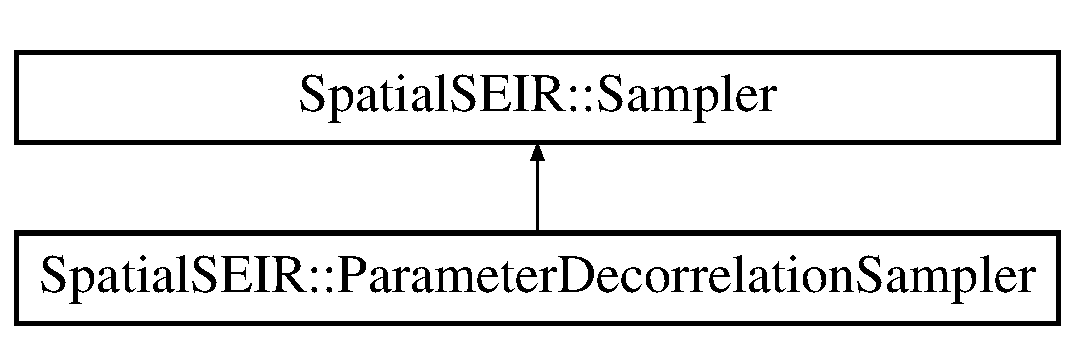
\includegraphics[height=2.000000cm]{classSpatialSEIR_1_1ParameterDecorrelationSampler}
\end{center}
\end{figure}
\subsection*{Public Member Functions}
\begin{DoxyCompactItemize}
\item 
\hyperlink{classSpatialSEIR_1_1ParameterDecorrelationSampler_af0361fd63d2070725aa4828b651375b7}{Parameter\-Decorrelation\-Sampler} (\hyperlink{classSpatialSEIR_1_1ModelContext}{Model\-Context} $\ast$\hyperlink{classSpatialSEIR_1_1ParameterDecorrelationSampler_a6d3abd37e28042269b7e46bd1dbf45f6}{context}, \hyperlink{classSpatialSEIR_1_1ParameterFullConditional}{Parameter\-Full\-Conditional} $\ast$\hyperlink{classSpatialSEIR_1_1ParameterDecorrelationSampler_a68fd577ec24b82e53d6f0e3db8227642}{param\-F\-C}, double $\ast$\hyperlink{classSpatialSEIR_1_1ParameterDecorrelationSampler_a4861d8e4ed1613da5b636535b1878ff5}{param}, \hyperlink{classSpatialSEIR_1_1CovariateMatrix}{Covariate\-Matrix} $\ast$\hyperlink{classSpatialSEIR_1_1ParameterDecorrelationSampler_afacba79f68960c5f287fe7551d39cb28}{proposal\-Matrix})
\item 
void \hyperlink{classSpatialSEIR_1_1ParameterDecorrelationSampler_ad1242cb40cf8a47667b3cbe82eff9c47}{draw\-Sample} ()
\item 
int \hyperlink{classSpatialSEIR_1_1ParameterDecorrelationSampler_ad3039ef7f917ec85fc210be2940b5da1}{get\-Sampler\-Type} ()
\item 
\hyperlink{classSpatialSEIR_1_1ParameterDecorrelationSampler_a5c10a71c09faa7026c2872a3cbc019d6}{$\sim$\-Parameter\-Decorrelation\-Sampler} ()
\end{DoxyCompactItemize}
\subsection*{Public Attributes}
\begin{DoxyCompactItemize}
\item 
double $\ast$$\ast$ \hyperlink{classSpatialSEIR_1_1ParameterDecorrelationSampler_a4861d8e4ed1613da5b636535b1878ff5}{param}
\item 
double $\ast$ \hyperlink{classSpatialSEIR_1_1ParameterDecorrelationSampler_a11fa351008038a247d6d4277a1e4dfe7}{proposal\-Cache}
\item 
double $\ast$ \hyperlink{classSpatialSEIR_1_1ParameterDecorrelationSampler_a4aee4558ad58aec311e280512acc8796}{proposal\-Cache2}
\item 
\hyperlink{classSpatialSEIR_1_1ModelContext}{Model\-Context} $\ast$$\ast$ \hyperlink{classSpatialSEIR_1_1ParameterDecorrelationSampler_a6d3abd37e28042269b7e46bd1dbf45f6}{context}
\item 
\hyperlink{classSpatialSEIR_1_1ParameterFullConditional}{Parameter\-Full\-Conditional} $\ast$$\ast$ \hyperlink{classSpatialSEIR_1_1ParameterDecorrelationSampler_a68fd577ec24b82e53d6f0e3db8227642}{param\-F\-C}
\item 
\hyperlink{classSpatialSEIR_1_1CovariateMatrix}{Covariate\-Matrix} $\ast$$\ast$ \hyperlink{classSpatialSEIR_1_1ParameterDecorrelationSampler_afacba79f68960c5f287fe7551d39cb28}{proposal\-Matrix}
\end{DoxyCompactItemize}


\subsection{Detailed Description}
The decorrelation sampler functions identically to the \hyperlink{classSpatialSEIR_1_1ParameterJointMetropolisSampler}{Parameter\-Joint\-Metropolis\-Sampler} class, except that proposals are drawn from the null space of the relevant design matrix. This can be useful when the explanatory variables are correlated. 

\subsection{Constructor \& Destructor Documentation}
\hypertarget{classSpatialSEIR_1_1ParameterDecorrelationSampler_af0361fd63d2070725aa4828b651375b7}{\index{Spatial\-S\-E\-I\-R\-::\-Parameter\-Decorrelation\-Sampler@{Spatial\-S\-E\-I\-R\-::\-Parameter\-Decorrelation\-Sampler}!Parameter\-Decorrelation\-Sampler@{Parameter\-Decorrelation\-Sampler}}
\index{Parameter\-Decorrelation\-Sampler@{Parameter\-Decorrelation\-Sampler}!SpatialSEIR::ParameterDecorrelationSampler@{Spatial\-S\-E\-I\-R\-::\-Parameter\-Decorrelation\-Sampler}}
\subsubsection[{Parameter\-Decorrelation\-Sampler}]{\setlength{\rightskip}{0pt plus 5cm}Spatial\-S\-E\-I\-R\-::\-Parameter\-Decorrelation\-Sampler\-::\-Parameter\-Decorrelation\-Sampler (
\begin{DoxyParamCaption}
\item[{{\bf Model\-Context} $\ast$}]{context, }
\item[{{\bf Parameter\-Full\-Conditional} $\ast$}]{param\-F\-C, }
\item[{double $\ast$}]{param, }
\item[{{\bf Covariate\-Matrix} $\ast$}]{proposal\-Matrix}
\end{DoxyParamCaption}
)}}\label{classSpatialSEIR_1_1ParameterDecorrelationSampler_af0361fd63d2070725aa4828b651375b7}
\hypertarget{classSpatialSEIR_1_1ParameterDecorrelationSampler_a5c10a71c09faa7026c2872a3cbc019d6}{\index{Spatial\-S\-E\-I\-R\-::\-Parameter\-Decorrelation\-Sampler@{Spatial\-S\-E\-I\-R\-::\-Parameter\-Decorrelation\-Sampler}!$\sim$\-Parameter\-Decorrelation\-Sampler@{$\sim$\-Parameter\-Decorrelation\-Sampler}}
\index{$\sim$\-Parameter\-Decorrelation\-Sampler@{$\sim$\-Parameter\-Decorrelation\-Sampler}!SpatialSEIR::ParameterDecorrelationSampler@{Spatial\-S\-E\-I\-R\-::\-Parameter\-Decorrelation\-Sampler}}
\subsubsection[{$\sim$\-Parameter\-Decorrelation\-Sampler}]{\setlength{\rightskip}{0pt plus 5cm}Spatial\-S\-E\-I\-R\-::\-Parameter\-Decorrelation\-Sampler\-::$\sim$\-Parameter\-Decorrelation\-Sampler (
\begin{DoxyParamCaption}
{}
\end{DoxyParamCaption}
)}}\label{classSpatialSEIR_1_1ParameterDecorrelationSampler_a5c10a71c09faa7026c2872a3cbc019d6}


\subsection{Member Function Documentation}
\hypertarget{classSpatialSEIR_1_1ParameterDecorrelationSampler_ad1242cb40cf8a47667b3cbe82eff9c47}{\index{Spatial\-S\-E\-I\-R\-::\-Parameter\-Decorrelation\-Sampler@{Spatial\-S\-E\-I\-R\-::\-Parameter\-Decorrelation\-Sampler}!draw\-Sample@{draw\-Sample}}
\index{draw\-Sample@{draw\-Sample}!SpatialSEIR::ParameterDecorrelationSampler@{Spatial\-S\-E\-I\-R\-::\-Parameter\-Decorrelation\-Sampler}}
\subsubsection[{draw\-Sample}]{\setlength{\rightskip}{0pt plus 5cm}void Spatial\-S\-E\-I\-R\-::\-Parameter\-Decorrelation\-Sampler\-::draw\-Sample (
\begin{DoxyParamCaption}
{}
\end{DoxyParamCaption}
)\hspace{0.3cm}{\ttfamily [virtual]}}}\label{classSpatialSEIR_1_1ParameterDecorrelationSampler_ad1242cb40cf8a47667b3cbe82eff9c47}


Implements \hyperlink{classSpatialSEIR_1_1Sampler_aa07a42b26cb62249c20c58e855a08657}{Spatial\-S\-E\-I\-R\-::\-Sampler}.

\hypertarget{classSpatialSEIR_1_1ParameterDecorrelationSampler_ad3039ef7f917ec85fc210be2940b5da1}{\index{Spatial\-S\-E\-I\-R\-::\-Parameter\-Decorrelation\-Sampler@{Spatial\-S\-E\-I\-R\-::\-Parameter\-Decorrelation\-Sampler}!get\-Sampler\-Type@{get\-Sampler\-Type}}
\index{get\-Sampler\-Type@{get\-Sampler\-Type}!SpatialSEIR::ParameterDecorrelationSampler@{Spatial\-S\-E\-I\-R\-::\-Parameter\-Decorrelation\-Sampler}}
\subsubsection[{get\-Sampler\-Type}]{\setlength{\rightskip}{0pt plus 5cm}int Spatial\-S\-E\-I\-R\-::\-Parameter\-Decorrelation\-Sampler\-::get\-Sampler\-Type (
\begin{DoxyParamCaption}
{}
\end{DoxyParamCaption}
)\hspace{0.3cm}{\ttfamily [virtual]}}}\label{classSpatialSEIR_1_1ParameterDecorrelationSampler_ad3039ef7f917ec85fc210be2940b5da1}


Implements \hyperlink{classSpatialSEIR_1_1Sampler_aaa79310ad809e6aeb25479849f322dda}{Spatial\-S\-E\-I\-R\-::\-Sampler}.



\subsection{Member Data Documentation}
\hypertarget{classSpatialSEIR_1_1ParameterDecorrelationSampler_a6d3abd37e28042269b7e46bd1dbf45f6}{\index{Spatial\-S\-E\-I\-R\-::\-Parameter\-Decorrelation\-Sampler@{Spatial\-S\-E\-I\-R\-::\-Parameter\-Decorrelation\-Sampler}!context@{context}}
\index{context@{context}!SpatialSEIR::ParameterDecorrelationSampler@{Spatial\-S\-E\-I\-R\-::\-Parameter\-Decorrelation\-Sampler}}
\subsubsection[{context}]{\setlength{\rightskip}{0pt plus 5cm}{\bf Model\-Context}$\ast$$\ast$ Spatial\-S\-E\-I\-R\-::\-Parameter\-Decorrelation\-Sampler\-::context}}\label{classSpatialSEIR_1_1ParameterDecorrelationSampler_a6d3abd37e28042269b7e46bd1dbf45f6}
\hypertarget{classSpatialSEIR_1_1ParameterDecorrelationSampler_a4861d8e4ed1613da5b636535b1878ff5}{\index{Spatial\-S\-E\-I\-R\-::\-Parameter\-Decorrelation\-Sampler@{Spatial\-S\-E\-I\-R\-::\-Parameter\-Decorrelation\-Sampler}!param@{param}}
\index{param@{param}!SpatialSEIR::ParameterDecorrelationSampler@{Spatial\-S\-E\-I\-R\-::\-Parameter\-Decorrelation\-Sampler}}
\subsubsection[{param}]{\setlength{\rightskip}{0pt plus 5cm}double$\ast$$\ast$ Spatial\-S\-E\-I\-R\-::\-Parameter\-Decorrelation\-Sampler\-::param}}\label{classSpatialSEIR_1_1ParameterDecorrelationSampler_a4861d8e4ed1613da5b636535b1878ff5}
\hypertarget{classSpatialSEIR_1_1ParameterDecorrelationSampler_a68fd577ec24b82e53d6f0e3db8227642}{\index{Spatial\-S\-E\-I\-R\-::\-Parameter\-Decorrelation\-Sampler@{Spatial\-S\-E\-I\-R\-::\-Parameter\-Decorrelation\-Sampler}!param\-F\-C@{param\-F\-C}}
\index{param\-F\-C@{param\-F\-C}!SpatialSEIR::ParameterDecorrelationSampler@{Spatial\-S\-E\-I\-R\-::\-Parameter\-Decorrelation\-Sampler}}
\subsubsection[{param\-F\-C}]{\setlength{\rightskip}{0pt plus 5cm}{\bf Parameter\-Full\-Conditional}$\ast$$\ast$ Spatial\-S\-E\-I\-R\-::\-Parameter\-Decorrelation\-Sampler\-::param\-F\-C}}\label{classSpatialSEIR_1_1ParameterDecorrelationSampler_a68fd577ec24b82e53d6f0e3db8227642}
\hypertarget{classSpatialSEIR_1_1ParameterDecorrelationSampler_a11fa351008038a247d6d4277a1e4dfe7}{\index{Spatial\-S\-E\-I\-R\-::\-Parameter\-Decorrelation\-Sampler@{Spatial\-S\-E\-I\-R\-::\-Parameter\-Decorrelation\-Sampler}!proposal\-Cache@{proposal\-Cache}}
\index{proposal\-Cache@{proposal\-Cache}!SpatialSEIR::ParameterDecorrelationSampler@{Spatial\-S\-E\-I\-R\-::\-Parameter\-Decorrelation\-Sampler}}
\subsubsection[{proposal\-Cache}]{\setlength{\rightskip}{0pt plus 5cm}double$\ast$ Spatial\-S\-E\-I\-R\-::\-Parameter\-Decorrelation\-Sampler\-::proposal\-Cache}}\label{classSpatialSEIR_1_1ParameterDecorrelationSampler_a11fa351008038a247d6d4277a1e4dfe7}
\hypertarget{classSpatialSEIR_1_1ParameterDecorrelationSampler_a4aee4558ad58aec311e280512acc8796}{\index{Spatial\-S\-E\-I\-R\-::\-Parameter\-Decorrelation\-Sampler@{Spatial\-S\-E\-I\-R\-::\-Parameter\-Decorrelation\-Sampler}!proposal\-Cache2@{proposal\-Cache2}}
\index{proposal\-Cache2@{proposal\-Cache2}!SpatialSEIR::ParameterDecorrelationSampler@{Spatial\-S\-E\-I\-R\-::\-Parameter\-Decorrelation\-Sampler}}
\subsubsection[{proposal\-Cache2}]{\setlength{\rightskip}{0pt plus 5cm}double$\ast$ Spatial\-S\-E\-I\-R\-::\-Parameter\-Decorrelation\-Sampler\-::proposal\-Cache2}}\label{classSpatialSEIR_1_1ParameterDecorrelationSampler_a4aee4558ad58aec311e280512acc8796}
\hypertarget{classSpatialSEIR_1_1ParameterDecorrelationSampler_afacba79f68960c5f287fe7551d39cb28}{\index{Spatial\-S\-E\-I\-R\-::\-Parameter\-Decorrelation\-Sampler@{Spatial\-S\-E\-I\-R\-::\-Parameter\-Decorrelation\-Sampler}!proposal\-Matrix@{proposal\-Matrix}}
\index{proposal\-Matrix@{proposal\-Matrix}!SpatialSEIR::ParameterDecorrelationSampler@{Spatial\-S\-E\-I\-R\-::\-Parameter\-Decorrelation\-Sampler}}
\subsubsection[{proposal\-Matrix}]{\setlength{\rightskip}{0pt plus 5cm}{\bf Covariate\-Matrix}$\ast$$\ast$ Spatial\-S\-E\-I\-R\-::\-Parameter\-Decorrelation\-Sampler\-::proposal\-Matrix}}\label{classSpatialSEIR_1_1ParameterDecorrelationSampler_afacba79f68960c5f287fe7551d39cb28}


The documentation for this class was generated from the following file\-:\begin{DoxyCompactItemize}
\item 
lib\-Spatial\-S\-E\-I\-R/include/\hyperlink{LSS__Samplers_8hpp}{L\-S\-S\-\_\-\-Samplers.\-hpp}\end{DoxyCompactItemize}

\hypertarget{classSpatialSEIR_1_1ParameterFullConditional}{\section{Spatial\-S\-E\-I\-R\-:\-:Parameter\-Full\-Conditional Class Reference}
\label{classSpatialSEIR_1_1ParameterFullConditional}\index{Spatial\-S\-E\-I\-R\-::\-Parameter\-Full\-Conditional@{Spatial\-S\-E\-I\-R\-::\-Parameter\-Full\-Conditional}}
}


{\ttfamily \#include $<$L\-S\-S\-\_\-\-Full\-Conditional.\-hpp$>$}

Inheritance diagram for Spatial\-S\-E\-I\-R\-:\-:Parameter\-Full\-Conditional\-:\begin{figure}[H]
\begin{center}
\leavevmode
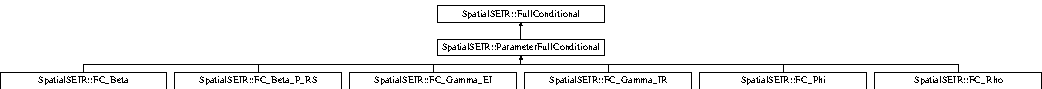
\includegraphics[height=1.201717cm]{classSpatialSEIR_1_1ParameterFullConditional}
\end{center}
\end{figure}
\subsection*{Public Member Functions}
\begin{DoxyCompactItemize}
\item 
virtual \hyperlink{classSpatialSEIR_1_1ParameterFullConditional_a8f86a572d719ff60c9620f17ae7d99bf}{$\sim$\-Parameter\-Full\-Conditional} ()
\item 
virtual int \hyperlink{classSpatialSEIR_1_1ParameterFullConditional_a186bd19fdeb52ca4522f56fb880201dd}{eval\-C\-P\-U} ()=0
\item 
virtual int \hyperlink{classSpatialSEIR_1_1ParameterFullConditional_ac4cfb13dace7f72e8136c45d9e959eec}{eval\-O\-C\-L} ()=0
\item 
virtual void \hyperlink{classSpatialSEIR_1_1ParameterFullConditional_a651e22b15782acb6bd80be12bd476693}{sample} (int verbose)=0
\item 
virtual long double \hyperlink{classSpatialSEIR_1_1ParameterFullConditional_a901368d385809e77179b9fa7532adfec}{get\-Value} ()=0
\item 
virtual void \hyperlink{classSpatialSEIR_1_1ParameterFullConditional_adf03f213e27d26f120b574d6dd86ffc3}{set\-Value} (long double value)=0
\item 
virtual int \hyperlink{classSpatialSEIR_1_1ParameterFullConditional_a65c39a2c3ca56e2f194b78cd362d35f9}{calculate\-Relevant\-Compartments} ()=0
\item 
virtual int \hyperlink{classSpatialSEIR_1_1ParameterFullConditional_af40754537736a64f58848e0368b001fb}{calculate\-Relevant\-Compartments\-\_\-\-O\-C\-L} ()=0
\item 
virtual double \hyperlink{classSpatialSEIR_1_1ParameterFullConditional_a0ddd01b6687b2617550a83f1feb5fa58}{acceptance\-Ratio} (int i)
\item 
void \hyperlink{classSpatialSEIR_1_1ParameterFullConditional_abae767010981e8f05e6c5e957739dabc}{update\-Sampling\-Parameters} (double desired\-Ratio, double target\-Width, double proportion\-Change)
\item 
int \hyperlink{classSpatialSEIR_1_1ParameterFullConditional_a2f2b5de88ed6e34e06b9b95413bfbdfc}{get\-Full\-Conditional\-Type} ()
\end{DoxyCompactItemize}
\subsection*{Public Attributes}
\begin{DoxyCompactItemize}
\item 
int $\ast$ \hyperlink{classSpatialSEIR_1_1ParameterFullConditional_a37e6c5effe2f808191fdc1eaf137270c}{var\-Len}
\end{DoxyCompactItemize}


\subsection{Detailed Description}
The \hyperlink{classSpatialSEIR_1_1ParameterFullConditional}{Parameter\-Full\-Conditional} class inherits the structure of \hyperlink{classSpatialSEIR_1_1FullConditional}{Full\-Conditional}, and provides sampling methods for all of the non-\/compartment parameters. These include the following\-:
\begin{DoxyEnumerate}
\item \hyperlink{classSpatialSEIR_1_1FC__Beta}{F\-C\-\_\-\-Beta}, the full conditional for the parameters controlling the exposure probability
\item \hyperlink{classSpatialSEIR_1_1FC__Beta__P__RS}{F\-C\-\_\-\-Beta\-\_\-\-P\-\_\-\-R\-S}, the full conditional for the parameters controlling the reinfection probability
\item \hyperlink{classSpatialSEIR_1_1FC__Rho}{F\-C\-\_\-\-Rho}, the full conditional for the spatial dependence parameter
\item F\-C\-\_\-\-P\-\_\-\-E\-I, the full conditional for the E to I transition probability
\item F\-C\-\_\-\-P\-\_\-\-I\-R, the full conditional for the I to R transition probability 
\end{DoxyEnumerate}

\subsection{Constructor \& Destructor Documentation}
\hypertarget{classSpatialSEIR_1_1ParameterFullConditional_a8f86a572d719ff60c9620f17ae7d99bf}{\index{Spatial\-S\-E\-I\-R\-::\-Parameter\-Full\-Conditional@{Spatial\-S\-E\-I\-R\-::\-Parameter\-Full\-Conditional}!$\sim$\-Parameter\-Full\-Conditional@{$\sim$\-Parameter\-Full\-Conditional}}
\index{$\sim$\-Parameter\-Full\-Conditional@{$\sim$\-Parameter\-Full\-Conditional}!SpatialSEIR::ParameterFullConditional@{Spatial\-S\-E\-I\-R\-::\-Parameter\-Full\-Conditional}}
\subsubsection[{$\sim$\-Parameter\-Full\-Conditional}]{\setlength{\rightskip}{0pt plus 5cm}virtual Spatial\-S\-E\-I\-R\-::\-Parameter\-Full\-Conditional\-::$\sim$\-Parameter\-Full\-Conditional (
\begin{DoxyParamCaption}
{}
\end{DoxyParamCaption}
)\hspace{0.3cm}{\ttfamily [inline]}, {\ttfamily [virtual]}}}\label{classSpatialSEIR_1_1ParameterFullConditional_a8f86a572d719ff60c9620f17ae7d99bf}


\subsection{Member Function Documentation}
\hypertarget{classSpatialSEIR_1_1ParameterFullConditional_a0ddd01b6687b2617550a83f1feb5fa58}{\index{Spatial\-S\-E\-I\-R\-::\-Parameter\-Full\-Conditional@{Spatial\-S\-E\-I\-R\-::\-Parameter\-Full\-Conditional}!acceptance\-Ratio@{acceptance\-Ratio}}
\index{acceptance\-Ratio@{acceptance\-Ratio}!SpatialSEIR::ParameterFullConditional@{Spatial\-S\-E\-I\-R\-::\-Parameter\-Full\-Conditional}}
\subsubsection[{acceptance\-Ratio}]{\setlength{\rightskip}{0pt plus 5cm}double Spatial\-S\-E\-I\-R\-::\-Parameter\-Full\-Conditional\-::acceptance\-Ratio (
\begin{DoxyParamCaption}
\item[{int}]{i}
\end{DoxyParamCaption}
)\hspace{0.3cm}{\ttfamily [virtual]}}}\label{classSpatialSEIR_1_1ParameterFullConditional_a0ddd01b6687b2617550a83f1feb5fa58}
\hypertarget{classSpatialSEIR_1_1ParameterFullConditional_a65c39a2c3ca56e2f194b78cd362d35f9}{\index{Spatial\-S\-E\-I\-R\-::\-Parameter\-Full\-Conditional@{Spatial\-S\-E\-I\-R\-::\-Parameter\-Full\-Conditional}!calculate\-Relevant\-Compartments@{calculate\-Relevant\-Compartments}}
\index{calculate\-Relevant\-Compartments@{calculate\-Relevant\-Compartments}!SpatialSEIR::ParameterFullConditional@{Spatial\-S\-E\-I\-R\-::\-Parameter\-Full\-Conditional}}
\subsubsection[{calculate\-Relevant\-Compartments}]{\setlength{\rightskip}{0pt plus 5cm}virtual int Spatial\-S\-E\-I\-R\-::\-Parameter\-Full\-Conditional\-::calculate\-Relevant\-Compartments (
\begin{DoxyParamCaption}
{}
\end{DoxyParamCaption}
)\hspace{0.3cm}{\ttfamily [pure virtual]}}}\label{classSpatialSEIR_1_1ParameterFullConditional_a65c39a2c3ca56e2f194b78cd362d35f9}


Implements \hyperlink{classSpatialSEIR_1_1FullConditional_a04c671e900a359f5a554817f21a99b5c}{Spatial\-S\-E\-I\-R\-::\-Full\-Conditional}.



Implemented in \hyperlink{classSpatialSEIR_1_1FC__Beta_ae5a92d2c0ebd51328296a8db45fc52ad}{Spatial\-S\-E\-I\-R\-::\-F\-C\-\_\-\-Beta}, \hyperlink{classSpatialSEIR_1_1FC__Beta__P__RS_a0edc8515a51962383536f8bf779ce194}{Spatial\-S\-E\-I\-R\-::\-F\-C\-\_\-\-Beta\-\_\-\-P\-\_\-\-R\-S}, \hyperlink{classSpatialSEIR_1_1FC__Gamma__IR_acdeddf0a6d53d2f10e7a12edf3924383}{Spatial\-S\-E\-I\-R\-::\-F\-C\-\_\-\-Gamma\-\_\-\-I\-R}, \hyperlink{classSpatialSEIR_1_1FC__Rho_aaed549dd0c459e96c1697f0578830455}{Spatial\-S\-E\-I\-R\-::\-F\-C\-\_\-\-Rho}, \hyperlink{classSpatialSEIR_1_1FC__Gamma__EI_ab2ac7a466661c568cf20ba89bced4ac2}{Spatial\-S\-E\-I\-R\-::\-F\-C\-\_\-\-Gamma\-\_\-\-E\-I}, and \hyperlink{classSpatialSEIR_1_1FC__Phi_a738d592a5efd1f6181b28b2f294d4f86}{Spatial\-S\-E\-I\-R\-::\-F\-C\-\_\-\-Phi}.

\hypertarget{classSpatialSEIR_1_1ParameterFullConditional_af40754537736a64f58848e0368b001fb}{\index{Spatial\-S\-E\-I\-R\-::\-Parameter\-Full\-Conditional@{Spatial\-S\-E\-I\-R\-::\-Parameter\-Full\-Conditional}!calculate\-Relevant\-Compartments\-\_\-\-O\-C\-L@{calculate\-Relevant\-Compartments\-\_\-\-O\-C\-L}}
\index{calculate\-Relevant\-Compartments\-\_\-\-O\-C\-L@{calculate\-Relevant\-Compartments\-\_\-\-O\-C\-L}!SpatialSEIR::ParameterFullConditional@{Spatial\-S\-E\-I\-R\-::\-Parameter\-Full\-Conditional}}
\subsubsection[{calculate\-Relevant\-Compartments\-\_\-\-O\-C\-L}]{\setlength{\rightskip}{0pt plus 5cm}virtual int Spatial\-S\-E\-I\-R\-::\-Parameter\-Full\-Conditional\-::calculate\-Relevant\-Compartments\-\_\-\-O\-C\-L (
\begin{DoxyParamCaption}
{}
\end{DoxyParamCaption}
)\hspace{0.3cm}{\ttfamily [pure virtual]}}}\label{classSpatialSEIR_1_1ParameterFullConditional_af40754537736a64f58848e0368b001fb}


Implements \hyperlink{classSpatialSEIR_1_1FullConditional_a77b75e8e1f62175aa0380a2e9aca3d46}{Spatial\-S\-E\-I\-R\-::\-Full\-Conditional}.



Implemented in \hyperlink{classSpatialSEIR_1_1FC__Beta_ac82fb2f313216cd5ebe611fbdf266416}{Spatial\-S\-E\-I\-R\-::\-F\-C\-\_\-\-Beta}, \hyperlink{classSpatialSEIR_1_1FC__Beta__P__RS_a156069877b44b2d1b3ecd94bf019bf6d}{Spatial\-S\-E\-I\-R\-::\-F\-C\-\_\-\-Beta\-\_\-\-P\-\_\-\-R\-S}, \hyperlink{classSpatialSEIR_1_1FC__Gamma__IR_a200f28e508a37bd50a8a0155fcd467c6}{Spatial\-S\-E\-I\-R\-::\-F\-C\-\_\-\-Gamma\-\_\-\-I\-R}, \hyperlink{classSpatialSEIR_1_1FC__Rho_a676f063fa861ac6297dc18c066bd7cf1}{Spatial\-S\-E\-I\-R\-::\-F\-C\-\_\-\-Rho}, \hyperlink{classSpatialSEIR_1_1FC__Gamma__EI_a1a10b7a7b3f0aa18af9bc60dcf17c150}{Spatial\-S\-E\-I\-R\-::\-F\-C\-\_\-\-Gamma\-\_\-\-E\-I}, and \hyperlink{classSpatialSEIR_1_1FC__Phi_acb391933ee8f5efd16d392b62d400933}{Spatial\-S\-E\-I\-R\-::\-F\-C\-\_\-\-Phi}.

\hypertarget{classSpatialSEIR_1_1ParameterFullConditional_a186bd19fdeb52ca4522f56fb880201dd}{\index{Spatial\-S\-E\-I\-R\-::\-Parameter\-Full\-Conditional@{Spatial\-S\-E\-I\-R\-::\-Parameter\-Full\-Conditional}!eval\-C\-P\-U@{eval\-C\-P\-U}}
\index{eval\-C\-P\-U@{eval\-C\-P\-U}!SpatialSEIR::ParameterFullConditional@{Spatial\-S\-E\-I\-R\-::\-Parameter\-Full\-Conditional}}
\subsubsection[{eval\-C\-P\-U}]{\setlength{\rightskip}{0pt plus 5cm}virtual int Spatial\-S\-E\-I\-R\-::\-Parameter\-Full\-Conditional\-::eval\-C\-P\-U (
\begin{DoxyParamCaption}
{}
\end{DoxyParamCaption}
)\hspace{0.3cm}{\ttfamily [pure virtual]}}}\label{classSpatialSEIR_1_1ParameterFullConditional_a186bd19fdeb52ca4522f56fb880201dd}


Implemented in \hyperlink{classSpatialSEIR_1_1FC__Beta_ae6f07bc7a0ef7ec660d1daadd060aad1}{Spatial\-S\-E\-I\-R\-::\-F\-C\-\_\-\-Beta}, \hyperlink{classSpatialSEIR_1_1FC__Beta__P__RS_a48e4e95be2abde217b71993c2b08e3da}{Spatial\-S\-E\-I\-R\-::\-F\-C\-\_\-\-Beta\-\_\-\-P\-\_\-\-R\-S}, \hyperlink{classSpatialSEIR_1_1FC__Gamma__IR_ac52b633a7878870a2e1adf059fb3c2ea}{Spatial\-S\-E\-I\-R\-::\-F\-C\-\_\-\-Gamma\-\_\-\-I\-R}, \hyperlink{classSpatialSEIR_1_1FC__Rho_a65e892331f9a129fc5840e7e40af70d4}{Spatial\-S\-E\-I\-R\-::\-F\-C\-\_\-\-Rho}, \hyperlink{classSpatialSEIR_1_1FC__Gamma__EI_ad04e240632b08359ae6d924d6d88fdde}{Spatial\-S\-E\-I\-R\-::\-F\-C\-\_\-\-Gamma\-\_\-\-E\-I}, and \hyperlink{classSpatialSEIR_1_1FC__Phi_a282b0c3778149a8f29364ff56543288d}{Spatial\-S\-E\-I\-R\-::\-F\-C\-\_\-\-Phi}.

\hypertarget{classSpatialSEIR_1_1ParameterFullConditional_ac4cfb13dace7f72e8136c45d9e959eec}{\index{Spatial\-S\-E\-I\-R\-::\-Parameter\-Full\-Conditional@{Spatial\-S\-E\-I\-R\-::\-Parameter\-Full\-Conditional}!eval\-O\-C\-L@{eval\-O\-C\-L}}
\index{eval\-O\-C\-L@{eval\-O\-C\-L}!SpatialSEIR::ParameterFullConditional@{Spatial\-S\-E\-I\-R\-::\-Parameter\-Full\-Conditional}}
\subsubsection[{eval\-O\-C\-L}]{\setlength{\rightskip}{0pt plus 5cm}virtual int Spatial\-S\-E\-I\-R\-::\-Parameter\-Full\-Conditional\-::eval\-O\-C\-L (
\begin{DoxyParamCaption}
{}
\end{DoxyParamCaption}
)\hspace{0.3cm}{\ttfamily [pure virtual]}}}\label{classSpatialSEIR_1_1ParameterFullConditional_ac4cfb13dace7f72e8136c45d9e959eec}


Implemented in \hyperlink{classSpatialSEIR_1_1FC__Beta_a882c2de38ecfa3a425010874dfacda0f}{Spatial\-S\-E\-I\-R\-::\-F\-C\-\_\-\-Beta}, \hyperlink{classSpatialSEIR_1_1FC__Beta__P__RS_ae51ca0e2ad990cd519fd62cf896c23ca}{Spatial\-S\-E\-I\-R\-::\-F\-C\-\_\-\-Beta\-\_\-\-P\-\_\-\-R\-S}, \hyperlink{classSpatialSEIR_1_1FC__Gamma__IR_a3423d47b7728892497a94407ecc37730}{Spatial\-S\-E\-I\-R\-::\-F\-C\-\_\-\-Gamma\-\_\-\-I\-R}, \hyperlink{classSpatialSEIR_1_1FC__Rho_a918b822d74871547519e5dc62c0bb25f}{Spatial\-S\-E\-I\-R\-::\-F\-C\-\_\-\-Rho}, \hyperlink{classSpatialSEIR_1_1FC__Gamma__EI_a30bbe6436e31914a36042488bd0ecd29}{Spatial\-S\-E\-I\-R\-::\-F\-C\-\_\-\-Gamma\-\_\-\-E\-I}, and \hyperlink{classSpatialSEIR_1_1FC__Phi_aa0683e5c52d7cfdaf106fe9d20348845}{Spatial\-S\-E\-I\-R\-::\-F\-C\-\_\-\-Phi}.

\hypertarget{classSpatialSEIR_1_1ParameterFullConditional_a2f2b5de88ed6e34e06b9b95413bfbdfc}{\index{Spatial\-S\-E\-I\-R\-::\-Parameter\-Full\-Conditional@{Spatial\-S\-E\-I\-R\-::\-Parameter\-Full\-Conditional}!get\-Full\-Conditional\-Type@{get\-Full\-Conditional\-Type}}
\index{get\-Full\-Conditional\-Type@{get\-Full\-Conditional\-Type}!SpatialSEIR::ParameterFullConditional@{Spatial\-S\-E\-I\-R\-::\-Parameter\-Full\-Conditional}}
\subsubsection[{get\-Full\-Conditional\-Type}]{\setlength{\rightskip}{0pt plus 5cm}int Spatial\-S\-E\-I\-R\-::\-Parameter\-Full\-Conditional\-::get\-Full\-Conditional\-Type (
\begin{DoxyParamCaption}
{}
\end{DoxyParamCaption}
)\hspace{0.3cm}{\ttfamily [virtual]}}}\label{classSpatialSEIR_1_1ParameterFullConditional_a2f2b5de88ed6e34e06b9b95413bfbdfc}
Identify as parameter full conditional 

Implements \hyperlink{classSpatialSEIR_1_1FullConditional_a680a2a8af1962a5a99191ff84acf78c5}{Spatial\-S\-E\-I\-R\-::\-Full\-Conditional}.

\hypertarget{classSpatialSEIR_1_1ParameterFullConditional_a901368d385809e77179b9fa7532adfec}{\index{Spatial\-S\-E\-I\-R\-::\-Parameter\-Full\-Conditional@{Spatial\-S\-E\-I\-R\-::\-Parameter\-Full\-Conditional}!get\-Value@{get\-Value}}
\index{get\-Value@{get\-Value}!SpatialSEIR::ParameterFullConditional@{Spatial\-S\-E\-I\-R\-::\-Parameter\-Full\-Conditional}}
\subsubsection[{get\-Value}]{\setlength{\rightskip}{0pt plus 5cm}virtual long double Spatial\-S\-E\-I\-R\-::\-Parameter\-Full\-Conditional\-::get\-Value (
\begin{DoxyParamCaption}
{}
\end{DoxyParamCaption}
)\hspace{0.3cm}{\ttfamily [pure virtual]}}}\label{classSpatialSEIR_1_1ParameterFullConditional_a901368d385809e77179b9fa7532adfec}


Implements \hyperlink{classSpatialSEIR_1_1FullConditional_abe67c774a66370686ee9dc6fe6f278f6}{Spatial\-S\-E\-I\-R\-::\-Full\-Conditional}.



Implemented in \hyperlink{classSpatialSEIR_1_1FC__Beta_a3d25a7f6965f0a899249b76d8bd9d75f}{Spatial\-S\-E\-I\-R\-::\-F\-C\-\_\-\-Beta}, \hyperlink{classSpatialSEIR_1_1FC__Beta__P__RS_a3017d4d02d954375869fe5d8e7e301ea}{Spatial\-S\-E\-I\-R\-::\-F\-C\-\_\-\-Beta\-\_\-\-P\-\_\-\-R\-S}, \hyperlink{classSpatialSEIR_1_1FC__Gamma__IR_a0895a64e8292e75141a4ad9ed1145e9d}{Spatial\-S\-E\-I\-R\-::\-F\-C\-\_\-\-Gamma\-\_\-\-I\-R}, \hyperlink{classSpatialSEIR_1_1FC__Rho_a2f6ad33590328ce079e7bc9b4f078907}{Spatial\-S\-E\-I\-R\-::\-F\-C\-\_\-\-Rho}, \hyperlink{classSpatialSEIR_1_1FC__Gamma__EI_ad33d614b75ea81d0a34eecbcec2fd406}{Spatial\-S\-E\-I\-R\-::\-F\-C\-\_\-\-Gamma\-\_\-\-E\-I}, and \hyperlink{classSpatialSEIR_1_1FC__Phi_a78d2ad18fd2696bdd91333b1b4d8984e}{Spatial\-S\-E\-I\-R\-::\-F\-C\-\_\-\-Phi}.

\hypertarget{classSpatialSEIR_1_1ParameterFullConditional_a651e22b15782acb6bd80be12bd476693}{\index{Spatial\-S\-E\-I\-R\-::\-Parameter\-Full\-Conditional@{Spatial\-S\-E\-I\-R\-::\-Parameter\-Full\-Conditional}!sample@{sample}}
\index{sample@{sample}!SpatialSEIR::ParameterFullConditional@{Spatial\-S\-E\-I\-R\-::\-Parameter\-Full\-Conditional}}
\subsubsection[{sample}]{\setlength{\rightskip}{0pt plus 5cm}virtual void Spatial\-S\-E\-I\-R\-::\-Parameter\-Full\-Conditional\-::sample (
\begin{DoxyParamCaption}
\item[{int}]{verbose}
\end{DoxyParamCaption}
)\hspace{0.3cm}{\ttfamily [pure virtual]}}}\label{classSpatialSEIR_1_1ParameterFullConditional_a651e22b15782acb6bd80be12bd476693}


Implements \hyperlink{classSpatialSEIR_1_1FullConditional_aac6928c9c2753acfc2c9e9bbe840ba82}{Spatial\-S\-E\-I\-R\-::\-Full\-Conditional}.



Implemented in \hyperlink{classSpatialSEIR_1_1FC__Beta_a96c2d002394eeee8cbcf7d06b8593dfc}{Spatial\-S\-E\-I\-R\-::\-F\-C\-\_\-\-Beta}, \hyperlink{classSpatialSEIR_1_1FC__Beta__P__RS_ae1a9ec2e9336c7c77106ff525d69ec64}{Spatial\-S\-E\-I\-R\-::\-F\-C\-\_\-\-Beta\-\_\-\-P\-\_\-\-R\-S}, \hyperlink{classSpatialSEIR_1_1FC__Gamma__IR_a1067c9b99b419d8c9d3566a5eb4b6d73}{Spatial\-S\-E\-I\-R\-::\-F\-C\-\_\-\-Gamma\-\_\-\-I\-R}, \hyperlink{classSpatialSEIR_1_1FC__Rho_a0d71fd3e8d9bd120991d60042c3e6a99}{Spatial\-S\-E\-I\-R\-::\-F\-C\-\_\-\-Rho}, \hyperlink{classSpatialSEIR_1_1FC__Gamma__EI_a33e0d2d52a85669f64fe058292ece1f8}{Spatial\-S\-E\-I\-R\-::\-F\-C\-\_\-\-Gamma\-\_\-\-E\-I}, and \hyperlink{classSpatialSEIR_1_1FC__Phi_ad01626131955f37c6abec78af34524dd}{Spatial\-S\-E\-I\-R\-::\-F\-C\-\_\-\-Phi}.

\hypertarget{classSpatialSEIR_1_1ParameterFullConditional_adf03f213e27d26f120b574d6dd86ffc3}{\index{Spatial\-S\-E\-I\-R\-::\-Parameter\-Full\-Conditional@{Spatial\-S\-E\-I\-R\-::\-Parameter\-Full\-Conditional}!set\-Value@{set\-Value}}
\index{set\-Value@{set\-Value}!SpatialSEIR::ParameterFullConditional@{Spatial\-S\-E\-I\-R\-::\-Parameter\-Full\-Conditional}}
\subsubsection[{set\-Value}]{\setlength{\rightskip}{0pt plus 5cm}virtual void Spatial\-S\-E\-I\-R\-::\-Parameter\-Full\-Conditional\-::set\-Value (
\begin{DoxyParamCaption}
\item[{long double}]{value}
\end{DoxyParamCaption}
)\hspace{0.3cm}{\ttfamily [pure virtual]}}}\label{classSpatialSEIR_1_1ParameterFullConditional_adf03f213e27d26f120b574d6dd86ffc3}


Implements \hyperlink{classSpatialSEIR_1_1FullConditional_a0834b0bb81ef4f7f368ba87fd784ff39}{Spatial\-S\-E\-I\-R\-::\-Full\-Conditional}.



Implemented in \hyperlink{classSpatialSEIR_1_1FC__Beta_a545ac3e04204a54d6f34c4356f474e42}{Spatial\-S\-E\-I\-R\-::\-F\-C\-\_\-\-Beta}, \hyperlink{classSpatialSEIR_1_1FC__Beta__P__RS_a788189d97ce2ffd40dc483a74ed63312}{Spatial\-S\-E\-I\-R\-::\-F\-C\-\_\-\-Beta\-\_\-\-P\-\_\-\-R\-S}, \hyperlink{classSpatialSEIR_1_1FC__Gamma__IR_a8517282f2fc24d52a00a426aa414f237}{Spatial\-S\-E\-I\-R\-::\-F\-C\-\_\-\-Gamma\-\_\-\-I\-R}, \hyperlink{classSpatialSEIR_1_1FC__Rho_a42dbc09ca0117f10ff27396cddb8dfa8}{Spatial\-S\-E\-I\-R\-::\-F\-C\-\_\-\-Rho}, \hyperlink{classSpatialSEIR_1_1FC__Gamma__EI_af1593c1841cea3c44e69d35af9640304}{Spatial\-S\-E\-I\-R\-::\-F\-C\-\_\-\-Gamma\-\_\-\-E\-I}, and \hyperlink{classSpatialSEIR_1_1FC__Phi_a71c23b1ea81880634e867786569b8b26}{Spatial\-S\-E\-I\-R\-::\-F\-C\-\_\-\-Phi}.

\hypertarget{classSpatialSEIR_1_1ParameterFullConditional_abae767010981e8f05e6c5e957739dabc}{\index{Spatial\-S\-E\-I\-R\-::\-Parameter\-Full\-Conditional@{Spatial\-S\-E\-I\-R\-::\-Parameter\-Full\-Conditional}!update\-Sampling\-Parameters@{update\-Sampling\-Parameters}}
\index{update\-Sampling\-Parameters@{update\-Sampling\-Parameters}!SpatialSEIR::ParameterFullConditional@{Spatial\-S\-E\-I\-R\-::\-Parameter\-Full\-Conditional}}
\subsubsection[{update\-Sampling\-Parameters}]{\setlength{\rightskip}{0pt plus 5cm}void Spatial\-S\-E\-I\-R\-::\-Parameter\-Full\-Conditional\-::update\-Sampling\-Parameters (
\begin{DoxyParamCaption}
\item[{double}]{desired\-Ratio, }
\item[{double}]{target\-Width, }
\item[{double}]{proportion\-Change}
\end{DoxyParamCaption}
)\hspace{0.3cm}{\ttfamily [virtual]}}}\label{classSpatialSEIR_1_1ParameterFullConditional_abae767010981e8f05e6c5e957739dabc}


Implements \hyperlink{classSpatialSEIR_1_1FullConditional_afd84b9273d641028453aefc06b342782}{Spatial\-S\-E\-I\-R\-::\-Full\-Conditional}.



\subsection{Member Data Documentation}
\hypertarget{classSpatialSEIR_1_1ParameterFullConditional_a37e6c5effe2f808191fdc1eaf137270c}{\index{Spatial\-S\-E\-I\-R\-::\-Parameter\-Full\-Conditional@{Spatial\-S\-E\-I\-R\-::\-Parameter\-Full\-Conditional}!var\-Len@{var\-Len}}
\index{var\-Len@{var\-Len}!SpatialSEIR::ParameterFullConditional@{Spatial\-S\-E\-I\-R\-::\-Parameter\-Full\-Conditional}}
\subsubsection[{var\-Len}]{\setlength{\rightskip}{0pt plus 5cm}int$\ast$ Spatial\-S\-E\-I\-R\-::\-Parameter\-Full\-Conditional\-::var\-Len}}\label{classSpatialSEIR_1_1ParameterFullConditional_a37e6c5effe2f808191fdc1eaf137270c}


The documentation for this class was generated from the following files\-:\begin{DoxyCompactItemize}
\item 
lib\-Spatial\-S\-E\-I\-R/include/\-Full\-Conditionals/\hyperlink{LSS__FullConditional_8hpp}{L\-S\-S\-\_\-\-Full\-Conditional.\-hpp}\item 
lib\-Spatial\-S\-E\-I\-R/src/\-Full\-Conditionals/\hyperlink{FullConditional_8cpp}{Full\-Conditional.\-cpp}\end{DoxyCompactItemize}

\hypertarget{classSpatialSEIR_1_1ParameterHybridSampler}{\section{Spatial\-S\-E\-I\-R\-:\-:Parameter\-Hybrid\-Sampler Class Reference}
\label{classSpatialSEIR_1_1ParameterHybridSampler}\index{Spatial\-S\-E\-I\-R\-::\-Parameter\-Hybrid\-Sampler@{Spatial\-S\-E\-I\-R\-::\-Parameter\-Hybrid\-Sampler}}
}


{\ttfamily \#include $<$L\-S\-S\-\_\-\-Samplers.\-hpp$>$}

Inheritance diagram for Spatial\-S\-E\-I\-R\-:\-:Parameter\-Hybrid\-Sampler\-:\begin{figure}[H]
\begin{center}
\leavevmode
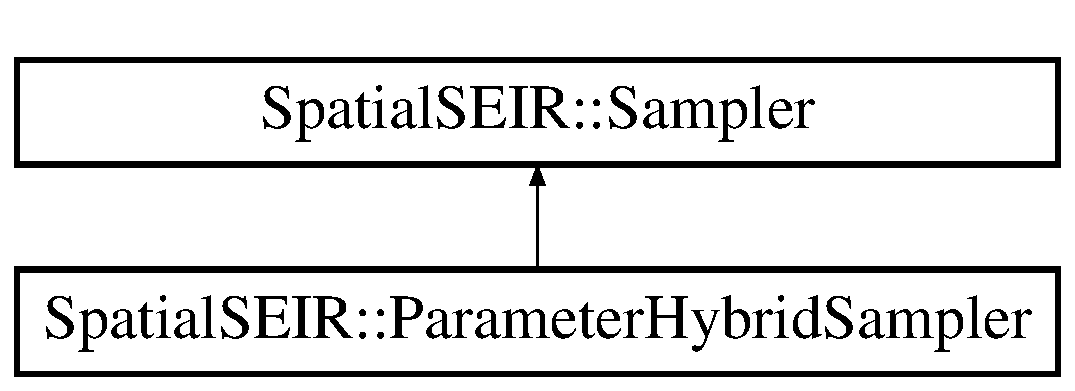
\includegraphics[height=2.000000cm]{classSpatialSEIR_1_1ParameterHybridSampler}
\end{center}
\end{figure}
\subsection*{Public Member Functions}
\begin{DoxyCompactItemize}
\item 
\hyperlink{classSpatialSEIR_1_1ParameterHybridSampler_a49a523f9cb8a4506d15febd00234d4ea}{Parameter\-Hybrid\-Sampler} (\hyperlink{classSpatialSEIR_1_1ModelContext}{Model\-Context} $\ast$\hyperlink{classSpatialSEIR_1_1ParameterHybridSampler_ad0bac901a073df234be795c3c989240b}{context}, std\-::vector$<$ \hyperlink{classSpatialSEIR_1_1ParameterFullConditional}{Parameter\-Full\-Conditional} $\ast$ $>$ \hyperlink{classSpatialSEIR_1_1ParameterHybridSampler_ae9ee223f22eaa7bc7c1a1ac0a046bbb5}{parameter\-Full\-Conditionals}, std\-::vector$<$ double $\ast$ $>$ \hyperlink{classSpatialSEIR_1_1ParameterHybridSampler_a78b4981910745b46803a7257e6cdc348}{parameters}, int \hyperlink{classSpatialSEIR_1_1ParameterHybridSampler_a09803b093b9f8864fc8923d41c25c5d5}{sampler\-Type})
\item 
void \hyperlink{classSpatialSEIR_1_1ParameterHybridSampler_a48bdd9605070604d06bcd576919a06f6}{draw\-Sample} ()
\item 
int \hyperlink{classSpatialSEIR_1_1ParameterHybridSampler_ae5c2d418521cc111a5f6e92e995f823c}{get\-Sampler\-Type} ()
\item 
\hyperlink{classSpatialSEIR_1_1ParameterHybridSampler_a85fe1867df7de09dd23f1b66f499419e}{$\sim$\-Parameter\-Hybrid\-Sampler} ()
\end{DoxyCompactItemize}
\subsection*{Public Attributes}
\begin{DoxyCompactItemize}
\item 
\hyperlink{classSpatialSEIR_1_1ModelContext}{Model\-Context} $\ast$$\ast$ \hyperlink{classSpatialSEIR_1_1ParameterHybridSampler_ad0bac901a073df234be795c3c989240b}{context}
\item 
int $\ast$ \hyperlink{classSpatialSEIR_1_1ParameterHybridSampler_a09803b093b9f8864fc8923d41c25c5d5}{sampler\-Type}
\item 
int $\ast$ \hyperlink{classSpatialSEIR_1_1ParameterHybridSampler_a0b875aabb2a3ea61945bc5354bfd151f}{total\-Param\-Size}
\item 
double $\ast$ \hyperlink{classSpatialSEIR_1_1ParameterHybridSampler_af6d11e07102ea7785b13252e2a9d2028}{parameter\-Cache}
\item 
std\-::vector\\*
$<$ \hyperlink{classSpatialSEIR_1_1ParameterFullConditional}{Parameter\-Full\-Conditional} $\ast$ $>$ $\ast$ \hyperlink{classSpatialSEIR_1_1ParameterHybridSampler_ae9ee223f22eaa7bc7c1a1ac0a046bbb5}{parameter\-Full\-Conditionals}
\item 
std\-::vector$<$ double $\ast$ $>$ $\ast$ \hyperlink{classSpatialSEIR_1_1ParameterHybridSampler_a78b4981910745b46803a7257e6cdc348}{parameters}
\end{DoxyCompactItemize}


\subsection{Detailed Description}
The \hyperlink{classSpatialSEIR_1_1ParameterHybridSampler}{Parameter\-Hybrid\-Sampler} class is an experimental approach to reducing autocorrelation by sampling parameters together. 

\subsection{Constructor \& Destructor Documentation}
\hypertarget{classSpatialSEIR_1_1ParameterHybridSampler_a49a523f9cb8a4506d15febd00234d4ea}{\index{Spatial\-S\-E\-I\-R\-::\-Parameter\-Hybrid\-Sampler@{Spatial\-S\-E\-I\-R\-::\-Parameter\-Hybrid\-Sampler}!Parameter\-Hybrid\-Sampler@{Parameter\-Hybrid\-Sampler}}
\index{Parameter\-Hybrid\-Sampler@{Parameter\-Hybrid\-Sampler}!SpatialSEIR::ParameterHybridSampler@{Spatial\-S\-E\-I\-R\-::\-Parameter\-Hybrid\-Sampler}}
\subsubsection[{Parameter\-Hybrid\-Sampler}]{\setlength{\rightskip}{0pt plus 5cm}Spatial\-S\-E\-I\-R\-::\-Parameter\-Hybrid\-Sampler\-::\-Parameter\-Hybrid\-Sampler (
\begin{DoxyParamCaption}
\item[{{\bf Model\-Context} $\ast$}]{context, }
\item[{std\-::vector$<$ {\bf Parameter\-Full\-Conditional} $\ast$ $>$}]{parameter\-Full\-Conditionals, }
\item[{std\-::vector$<$ double $\ast$ $>$}]{parameters, }
\item[{int}]{sampler\-Type}
\end{DoxyParamCaption}
)}}\label{classSpatialSEIR_1_1ParameterHybridSampler_a49a523f9cb8a4506d15febd00234d4ea}
\hypertarget{classSpatialSEIR_1_1ParameterHybridSampler_a85fe1867df7de09dd23f1b66f499419e}{\index{Spatial\-S\-E\-I\-R\-::\-Parameter\-Hybrid\-Sampler@{Spatial\-S\-E\-I\-R\-::\-Parameter\-Hybrid\-Sampler}!$\sim$\-Parameter\-Hybrid\-Sampler@{$\sim$\-Parameter\-Hybrid\-Sampler}}
\index{$\sim$\-Parameter\-Hybrid\-Sampler@{$\sim$\-Parameter\-Hybrid\-Sampler}!SpatialSEIR::ParameterHybridSampler@{Spatial\-S\-E\-I\-R\-::\-Parameter\-Hybrid\-Sampler}}
\subsubsection[{$\sim$\-Parameter\-Hybrid\-Sampler}]{\setlength{\rightskip}{0pt plus 5cm}Spatial\-S\-E\-I\-R\-::\-Parameter\-Hybrid\-Sampler\-::$\sim$\-Parameter\-Hybrid\-Sampler (
\begin{DoxyParamCaption}
{}
\end{DoxyParamCaption}
)}}\label{classSpatialSEIR_1_1ParameterHybridSampler_a85fe1867df7de09dd23f1b66f499419e}


\subsection{Member Function Documentation}
\hypertarget{classSpatialSEIR_1_1ParameterHybridSampler_a48bdd9605070604d06bcd576919a06f6}{\index{Spatial\-S\-E\-I\-R\-::\-Parameter\-Hybrid\-Sampler@{Spatial\-S\-E\-I\-R\-::\-Parameter\-Hybrid\-Sampler}!draw\-Sample@{draw\-Sample}}
\index{draw\-Sample@{draw\-Sample}!SpatialSEIR::ParameterHybridSampler@{Spatial\-S\-E\-I\-R\-::\-Parameter\-Hybrid\-Sampler}}
\subsubsection[{draw\-Sample}]{\setlength{\rightskip}{0pt plus 5cm}void Spatial\-S\-E\-I\-R\-::\-Parameter\-Hybrid\-Sampler\-::draw\-Sample (
\begin{DoxyParamCaption}
{}
\end{DoxyParamCaption}
)\hspace{0.3cm}{\ttfamily [virtual]}}}\label{classSpatialSEIR_1_1ParameterHybridSampler_a48bdd9605070604d06bcd576919a06f6}


Implements \hyperlink{classSpatialSEIR_1_1Sampler_aa07a42b26cb62249c20c58e855a08657}{Spatial\-S\-E\-I\-R\-::\-Sampler}.

\hypertarget{classSpatialSEIR_1_1ParameterHybridSampler_ae5c2d418521cc111a5f6e92e995f823c}{\index{Spatial\-S\-E\-I\-R\-::\-Parameter\-Hybrid\-Sampler@{Spatial\-S\-E\-I\-R\-::\-Parameter\-Hybrid\-Sampler}!get\-Sampler\-Type@{get\-Sampler\-Type}}
\index{get\-Sampler\-Type@{get\-Sampler\-Type}!SpatialSEIR::ParameterHybridSampler@{Spatial\-S\-E\-I\-R\-::\-Parameter\-Hybrid\-Sampler}}
\subsubsection[{get\-Sampler\-Type}]{\setlength{\rightskip}{0pt plus 5cm}int Spatial\-S\-E\-I\-R\-::\-Parameter\-Hybrid\-Sampler\-::get\-Sampler\-Type (
\begin{DoxyParamCaption}
{}
\end{DoxyParamCaption}
)\hspace{0.3cm}{\ttfamily [virtual]}}}\label{classSpatialSEIR_1_1ParameterHybridSampler_ae5c2d418521cc111a5f6e92e995f823c}


Implements \hyperlink{classSpatialSEIR_1_1Sampler_aaa79310ad809e6aeb25479849f322dda}{Spatial\-S\-E\-I\-R\-::\-Sampler}.



\subsection{Member Data Documentation}
\hypertarget{classSpatialSEIR_1_1ParameterHybridSampler_ad0bac901a073df234be795c3c989240b}{\index{Spatial\-S\-E\-I\-R\-::\-Parameter\-Hybrid\-Sampler@{Spatial\-S\-E\-I\-R\-::\-Parameter\-Hybrid\-Sampler}!context@{context}}
\index{context@{context}!SpatialSEIR::ParameterHybridSampler@{Spatial\-S\-E\-I\-R\-::\-Parameter\-Hybrid\-Sampler}}
\subsubsection[{context}]{\setlength{\rightskip}{0pt plus 5cm}{\bf Model\-Context}$\ast$$\ast$ Spatial\-S\-E\-I\-R\-::\-Parameter\-Hybrid\-Sampler\-::context}}\label{classSpatialSEIR_1_1ParameterHybridSampler_ad0bac901a073df234be795c3c989240b}
\hypertarget{classSpatialSEIR_1_1ParameterHybridSampler_af6d11e07102ea7785b13252e2a9d2028}{\index{Spatial\-S\-E\-I\-R\-::\-Parameter\-Hybrid\-Sampler@{Spatial\-S\-E\-I\-R\-::\-Parameter\-Hybrid\-Sampler}!parameter\-Cache@{parameter\-Cache}}
\index{parameter\-Cache@{parameter\-Cache}!SpatialSEIR::ParameterHybridSampler@{Spatial\-S\-E\-I\-R\-::\-Parameter\-Hybrid\-Sampler}}
\subsubsection[{parameter\-Cache}]{\setlength{\rightskip}{0pt plus 5cm}double$\ast$ Spatial\-S\-E\-I\-R\-::\-Parameter\-Hybrid\-Sampler\-::parameter\-Cache}}\label{classSpatialSEIR_1_1ParameterHybridSampler_af6d11e07102ea7785b13252e2a9d2028}
\hypertarget{classSpatialSEIR_1_1ParameterHybridSampler_ae9ee223f22eaa7bc7c1a1ac0a046bbb5}{\index{Spatial\-S\-E\-I\-R\-::\-Parameter\-Hybrid\-Sampler@{Spatial\-S\-E\-I\-R\-::\-Parameter\-Hybrid\-Sampler}!parameter\-Full\-Conditionals@{parameter\-Full\-Conditionals}}
\index{parameter\-Full\-Conditionals@{parameter\-Full\-Conditionals}!SpatialSEIR::ParameterHybridSampler@{Spatial\-S\-E\-I\-R\-::\-Parameter\-Hybrid\-Sampler}}
\subsubsection[{parameter\-Full\-Conditionals}]{\setlength{\rightskip}{0pt plus 5cm}std\-::vector$<${\bf Parameter\-Full\-Conditional}$\ast$$>$$\ast$ Spatial\-S\-E\-I\-R\-::\-Parameter\-Hybrid\-Sampler\-::parameter\-Full\-Conditionals}}\label{classSpatialSEIR_1_1ParameterHybridSampler_ae9ee223f22eaa7bc7c1a1ac0a046bbb5}
\hypertarget{classSpatialSEIR_1_1ParameterHybridSampler_a78b4981910745b46803a7257e6cdc348}{\index{Spatial\-S\-E\-I\-R\-::\-Parameter\-Hybrid\-Sampler@{Spatial\-S\-E\-I\-R\-::\-Parameter\-Hybrid\-Sampler}!parameters@{parameters}}
\index{parameters@{parameters}!SpatialSEIR::ParameterHybridSampler@{Spatial\-S\-E\-I\-R\-::\-Parameter\-Hybrid\-Sampler}}
\subsubsection[{parameters}]{\setlength{\rightskip}{0pt plus 5cm}std\-::vector$<$double$\ast$$>$$\ast$ Spatial\-S\-E\-I\-R\-::\-Parameter\-Hybrid\-Sampler\-::parameters}}\label{classSpatialSEIR_1_1ParameterHybridSampler_a78b4981910745b46803a7257e6cdc348}
\hypertarget{classSpatialSEIR_1_1ParameterHybridSampler_a09803b093b9f8864fc8923d41c25c5d5}{\index{Spatial\-S\-E\-I\-R\-::\-Parameter\-Hybrid\-Sampler@{Spatial\-S\-E\-I\-R\-::\-Parameter\-Hybrid\-Sampler}!sampler\-Type@{sampler\-Type}}
\index{sampler\-Type@{sampler\-Type}!SpatialSEIR::ParameterHybridSampler@{Spatial\-S\-E\-I\-R\-::\-Parameter\-Hybrid\-Sampler}}
\subsubsection[{sampler\-Type}]{\setlength{\rightskip}{0pt plus 5cm}int$\ast$ Spatial\-S\-E\-I\-R\-::\-Parameter\-Hybrid\-Sampler\-::sampler\-Type}}\label{classSpatialSEIR_1_1ParameterHybridSampler_a09803b093b9f8864fc8923d41c25c5d5}
\hypertarget{classSpatialSEIR_1_1ParameterHybridSampler_a0b875aabb2a3ea61945bc5354bfd151f}{\index{Spatial\-S\-E\-I\-R\-::\-Parameter\-Hybrid\-Sampler@{Spatial\-S\-E\-I\-R\-::\-Parameter\-Hybrid\-Sampler}!total\-Param\-Size@{total\-Param\-Size}}
\index{total\-Param\-Size@{total\-Param\-Size}!SpatialSEIR::ParameterHybridSampler@{Spatial\-S\-E\-I\-R\-::\-Parameter\-Hybrid\-Sampler}}
\subsubsection[{total\-Param\-Size}]{\setlength{\rightskip}{0pt plus 5cm}int$\ast$ Spatial\-S\-E\-I\-R\-::\-Parameter\-Hybrid\-Sampler\-::total\-Param\-Size}}\label{classSpatialSEIR_1_1ParameterHybridSampler_a0b875aabb2a3ea61945bc5354bfd151f}


The documentation for this class was generated from the following file\-:\begin{DoxyCompactItemize}
\item 
lib\-Spatial\-S\-E\-I\-R/include/\hyperlink{LSS__Samplers_8hpp}{L\-S\-S\-\_\-\-Samplers.\-hpp}\end{DoxyCompactItemize}

\hypertarget{classSpatialSEIR_1_1ParameterJointMetropolisSampler}{\section{Spatial\-S\-E\-I\-R\-:\-:Parameter\-Joint\-Metropolis\-Sampler Class Reference}
\label{classSpatialSEIR_1_1ParameterJointMetropolisSampler}\index{Spatial\-S\-E\-I\-R\-::\-Parameter\-Joint\-Metropolis\-Sampler@{Spatial\-S\-E\-I\-R\-::\-Parameter\-Joint\-Metropolis\-Sampler}}
}


{\ttfamily \#include $<$L\-S\-S\-\_\-\-Samplers.\-hpp$>$}

Inheritance diagram for Spatial\-S\-E\-I\-R\-:\-:Parameter\-Joint\-Metropolis\-Sampler\-:\begin{figure}[H]
\begin{center}
\leavevmode
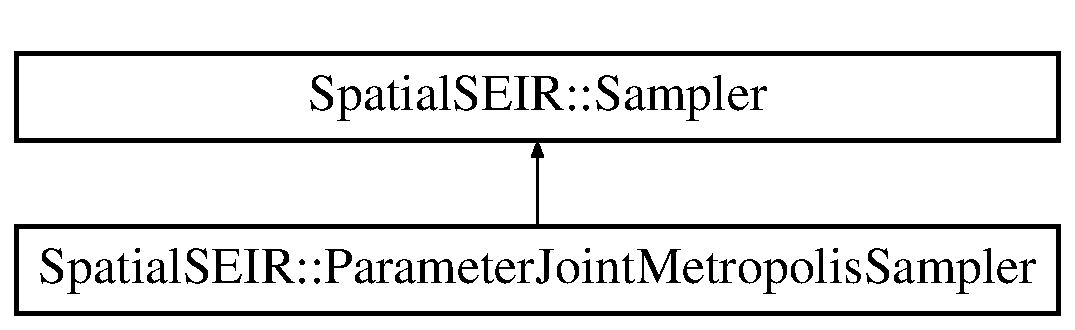
\includegraphics[height=2.000000cm]{classSpatialSEIR_1_1ParameterJointMetropolisSampler}
\end{center}
\end{figure}
\subsection*{Public Member Functions}
\begin{DoxyCompactItemize}
\item 
\hyperlink{classSpatialSEIR_1_1ParameterJointMetropolisSampler_a86159a1b20311138c9b96339c6512276}{Parameter\-Joint\-Metropolis\-Sampler} (\hyperlink{classSpatialSEIR_1_1ModelContext}{Model\-Context} $\ast$\hyperlink{classSpatialSEIR_1_1ParameterJointMetropolisSampler_a342dea442e235b1deefe2c16dd3e95e8}{context}, \hyperlink{classSpatialSEIR_1_1ParameterFullConditional}{Parameter\-Full\-Conditional} $\ast$\hyperlink{classSpatialSEIR_1_1ParameterJointMetropolisSampler_a2ceafdb76768003ed5eaa4b22ca6afeb}{param\-F\-C}, double $\ast$\hyperlink{classSpatialSEIR_1_1ParameterJointMetropolisSampler_afead5b10ba404c235e7042670c350eeb}{param})
\item 
void \hyperlink{classSpatialSEIR_1_1ParameterJointMetropolisSampler_a1224be64e1a5e46290c6f2d95b13fec7}{draw\-Sample} ()
\item 
int \hyperlink{classSpatialSEIR_1_1ParameterJointMetropolisSampler_a5684e2933ff1fab50e1761450ba41897}{get\-Sampler\-Type} ()
\item 
\hyperlink{classSpatialSEIR_1_1ParameterJointMetropolisSampler_a726371badc62d132c336759f9ca965be}{$\sim$\-Parameter\-Joint\-Metropolis\-Sampler} ()
\end{DoxyCompactItemize}
\subsection*{Public Attributes}
\begin{DoxyCompactItemize}
\item 
double $\ast$$\ast$ \hyperlink{classSpatialSEIR_1_1ParameterJointMetropolisSampler_afead5b10ba404c235e7042670c350eeb}{param}
\item 
\hyperlink{classSpatialSEIR_1_1ModelContext}{Model\-Context} $\ast$$\ast$ \hyperlink{classSpatialSEIR_1_1ParameterJointMetropolisSampler_a342dea442e235b1deefe2c16dd3e95e8}{context}
\item 
\hyperlink{classSpatialSEIR_1_1ParameterFullConditional}{Parameter\-Full\-Conditional} $\ast$$\ast$ \hyperlink{classSpatialSEIR_1_1ParameterJointMetropolisSampler_a2ceafdb76768003ed5eaa4b22ca6afeb}{param\-F\-C}
\end{DoxyCompactItemize}


\subsection{Detailed Description}
The \hyperlink{classSpatialSEIR_1_1ParameterJointMetropolisSampler}{Parameter\-Joint\-Metropolis\-Sampler} uses full vector Metropolis proposals to sample non Compartmental\-Matrix parameters. 

\subsection{Constructor \& Destructor Documentation}
\hypertarget{classSpatialSEIR_1_1ParameterJointMetropolisSampler_a86159a1b20311138c9b96339c6512276}{\index{Spatial\-S\-E\-I\-R\-::\-Parameter\-Joint\-Metropolis\-Sampler@{Spatial\-S\-E\-I\-R\-::\-Parameter\-Joint\-Metropolis\-Sampler}!Parameter\-Joint\-Metropolis\-Sampler@{Parameter\-Joint\-Metropolis\-Sampler}}
\index{Parameter\-Joint\-Metropolis\-Sampler@{Parameter\-Joint\-Metropolis\-Sampler}!SpatialSEIR::ParameterJointMetropolisSampler@{Spatial\-S\-E\-I\-R\-::\-Parameter\-Joint\-Metropolis\-Sampler}}
\subsubsection[{Parameter\-Joint\-Metropolis\-Sampler}]{\setlength{\rightskip}{0pt plus 5cm}Spatial\-S\-E\-I\-R\-::\-Parameter\-Joint\-Metropolis\-Sampler\-::\-Parameter\-Joint\-Metropolis\-Sampler (
\begin{DoxyParamCaption}
\item[{{\bf Model\-Context} $\ast$}]{context, }
\item[{{\bf Parameter\-Full\-Conditional} $\ast$}]{param\-F\-C, }
\item[{double $\ast$}]{param}
\end{DoxyParamCaption}
)}}\label{classSpatialSEIR_1_1ParameterJointMetropolisSampler_a86159a1b20311138c9b96339c6512276}
\hypertarget{classSpatialSEIR_1_1ParameterJointMetropolisSampler_a726371badc62d132c336759f9ca965be}{\index{Spatial\-S\-E\-I\-R\-::\-Parameter\-Joint\-Metropolis\-Sampler@{Spatial\-S\-E\-I\-R\-::\-Parameter\-Joint\-Metropolis\-Sampler}!$\sim$\-Parameter\-Joint\-Metropolis\-Sampler@{$\sim$\-Parameter\-Joint\-Metropolis\-Sampler}}
\index{$\sim$\-Parameter\-Joint\-Metropolis\-Sampler@{$\sim$\-Parameter\-Joint\-Metropolis\-Sampler}!SpatialSEIR::ParameterJointMetropolisSampler@{Spatial\-S\-E\-I\-R\-::\-Parameter\-Joint\-Metropolis\-Sampler}}
\subsubsection[{$\sim$\-Parameter\-Joint\-Metropolis\-Sampler}]{\setlength{\rightskip}{0pt plus 5cm}Spatial\-S\-E\-I\-R\-::\-Parameter\-Joint\-Metropolis\-Sampler\-::$\sim$\-Parameter\-Joint\-Metropolis\-Sampler (
\begin{DoxyParamCaption}
{}
\end{DoxyParamCaption}
)}}\label{classSpatialSEIR_1_1ParameterJointMetropolisSampler_a726371badc62d132c336759f9ca965be}


\subsection{Member Function Documentation}
\hypertarget{classSpatialSEIR_1_1ParameterJointMetropolisSampler_a1224be64e1a5e46290c6f2d95b13fec7}{\index{Spatial\-S\-E\-I\-R\-::\-Parameter\-Joint\-Metropolis\-Sampler@{Spatial\-S\-E\-I\-R\-::\-Parameter\-Joint\-Metropolis\-Sampler}!draw\-Sample@{draw\-Sample}}
\index{draw\-Sample@{draw\-Sample}!SpatialSEIR::ParameterJointMetropolisSampler@{Spatial\-S\-E\-I\-R\-::\-Parameter\-Joint\-Metropolis\-Sampler}}
\subsubsection[{draw\-Sample}]{\setlength{\rightskip}{0pt plus 5cm}void Spatial\-S\-E\-I\-R\-::\-Parameter\-Joint\-Metropolis\-Sampler\-::draw\-Sample (
\begin{DoxyParamCaption}
{}
\end{DoxyParamCaption}
)\hspace{0.3cm}{\ttfamily [virtual]}}}\label{classSpatialSEIR_1_1ParameterJointMetropolisSampler_a1224be64e1a5e46290c6f2d95b13fec7}


Implements \hyperlink{classSpatialSEIR_1_1Sampler_aa07a42b26cb62249c20c58e855a08657}{Spatial\-S\-E\-I\-R\-::\-Sampler}.

\hypertarget{classSpatialSEIR_1_1ParameterJointMetropolisSampler_a5684e2933ff1fab50e1761450ba41897}{\index{Spatial\-S\-E\-I\-R\-::\-Parameter\-Joint\-Metropolis\-Sampler@{Spatial\-S\-E\-I\-R\-::\-Parameter\-Joint\-Metropolis\-Sampler}!get\-Sampler\-Type@{get\-Sampler\-Type}}
\index{get\-Sampler\-Type@{get\-Sampler\-Type}!SpatialSEIR::ParameterJointMetropolisSampler@{Spatial\-S\-E\-I\-R\-::\-Parameter\-Joint\-Metropolis\-Sampler}}
\subsubsection[{get\-Sampler\-Type}]{\setlength{\rightskip}{0pt plus 5cm}int Spatial\-S\-E\-I\-R\-::\-Parameter\-Joint\-Metropolis\-Sampler\-::get\-Sampler\-Type (
\begin{DoxyParamCaption}
{}
\end{DoxyParamCaption}
)\hspace{0.3cm}{\ttfamily [virtual]}}}\label{classSpatialSEIR_1_1ParameterJointMetropolisSampler_a5684e2933ff1fab50e1761450ba41897}


Implements \hyperlink{classSpatialSEIR_1_1Sampler_aaa79310ad809e6aeb25479849f322dda}{Spatial\-S\-E\-I\-R\-::\-Sampler}.



\subsection{Member Data Documentation}
\hypertarget{classSpatialSEIR_1_1ParameterJointMetropolisSampler_a342dea442e235b1deefe2c16dd3e95e8}{\index{Spatial\-S\-E\-I\-R\-::\-Parameter\-Joint\-Metropolis\-Sampler@{Spatial\-S\-E\-I\-R\-::\-Parameter\-Joint\-Metropolis\-Sampler}!context@{context}}
\index{context@{context}!SpatialSEIR::ParameterJointMetropolisSampler@{Spatial\-S\-E\-I\-R\-::\-Parameter\-Joint\-Metropolis\-Sampler}}
\subsubsection[{context}]{\setlength{\rightskip}{0pt plus 5cm}{\bf Model\-Context}$\ast$$\ast$ Spatial\-S\-E\-I\-R\-::\-Parameter\-Joint\-Metropolis\-Sampler\-::context}}\label{classSpatialSEIR_1_1ParameterJointMetropolisSampler_a342dea442e235b1deefe2c16dd3e95e8}
\hypertarget{classSpatialSEIR_1_1ParameterJointMetropolisSampler_afead5b10ba404c235e7042670c350eeb}{\index{Spatial\-S\-E\-I\-R\-::\-Parameter\-Joint\-Metropolis\-Sampler@{Spatial\-S\-E\-I\-R\-::\-Parameter\-Joint\-Metropolis\-Sampler}!param@{param}}
\index{param@{param}!SpatialSEIR::ParameterJointMetropolisSampler@{Spatial\-S\-E\-I\-R\-::\-Parameter\-Joint\-Metropolis\-Sampler}}
\subsubsection[{param}]{\setlength{\rightskip}{0pt plus 5cm}double$\ast$$\ast$ Spatial\-S\-E\-I\-R\-::\-Parameter\-Joint\-Metropolis\-Sampler\-::param}}\label{classSpatialSEIR_1_1ParameterJointMetropolisSampler_afead5b10ba404c235e7042670c350eeb}
\hypertarget{classSpatialSEIR_1_1ParameterJointMetropolisSampler_a2ceafdb76768003ed5eaa4b22ca6afeb}{\index{Spatial\-S\-E\-I\-R\-::\-Parameter\-Joint\-Metropolis\-Sampler@{Spatial\-S\-E\-I\-R\-::\-Parameter\-Joint\-Metropolis\-Sampler}!param\-F\-C@{param\-F\-C}}
\index{param\-F\-C@{param\-F\-C}!SpatialSEIR::ParameterJointMetropolisSampler@{Spatial\-S\-E\-I\-R\-::\-Parameter\-Joint\-Metropolis\-Sampler}}
\subsubsection[{param\-F\-C}]{\setlength{\rightskip}{0pt plus 5cm}{\bf Parameter\-Full\-Conditional}$\ast$$\ast$ Spatial\-S\-E\-I\-R\-::\-Parameter\-Joint\-Metropolis\-Sampler\-::param\-F\-C}}\label{classSpatialSEIR_1_1ParameterJointMetropolisSampler_a2ceafdb76768003ed5eaa4b22ca6afeb}


The documentation for this class was generated from the following file\-:\begin{DoxyCompactItemize}
\item 
lib\-Spatial\-S\-E\-I\-R/include/\hyperlink{LSS__Samplers_8hpp}{L\-S\-S\-\_\-\-Samplers.\-hpp}\end{DoxyCompactItemize}

\hypertarget{classSpatialSEIR_1_1ParameterJointMetropolisSampler__OCL}{\section{Spatial\-S\-E\-I\-R\-:\-:Parameter\-Joint\-Metropolis\-Sampler\-\_\-\-O\-C\-L Class Reference}
\label{classSpatialSEIR_1_1ParameterJointMetropolisSampler__OCL}\index{Spatial\-S\-E\-I\-R\-::\-Parameter\-Joint\-Metropolis\-Sampler\-\_\-\-O\-C\-L@{Spatial\-S\-E\-I\-R\-::\-Parameter\-Joint\-Metropolis\-Sampler\-\_\-\-O\-C\-L}}
}


{\ttfamily \#include $<$L\-S\-S\-\_\-\-Samplers.\-hpp$>$}

Inheritance diagram for Spatial\-S\-E\-I\-R\-:\-:Parameter\-Joint\-Metropolis\-Sampler\-\_\-\-O\-C\-L\-:\begin{figure}[H]
\begin{center}
\leavevmode
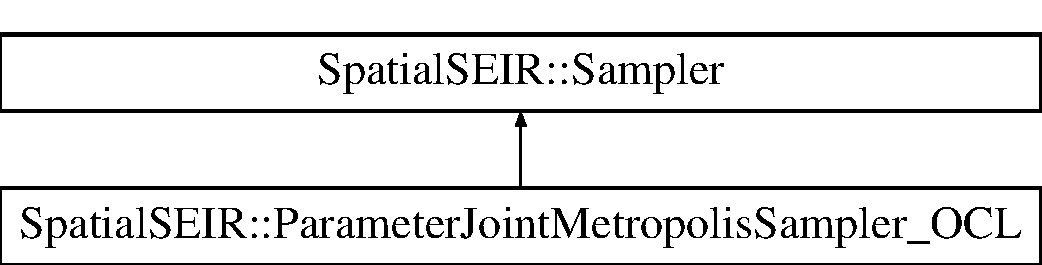
\includegraphics[height=2.000000cm]{classSpatialSEIR_1_1ParameterJointMetropolisSampler__OCL}
\end{center}
\end{figure}
\subsection*{Public Member Functions}
\begin{DoxyCompactItemize}
\item 
\hyperlink{classSpatialSEIR_1_1ParameterJointMetropolisSampler__OCL_a8b74295190dc338730bf3ed73375b100}{Parameter\-Joint\-Metropolis\-Sampler\-\_\-\-O\-C\-L} (\hyperlink{classSpatialSEIR_1_1ModelContext}{Model\-Context} $\ast$\hyperlink{classSpatialSEIR_1_1ParameterJointMetropolisSampler__OCL_acce9d454489373f0549af4f15dade51a}{context}, \hyperlink{classSpatialSEIR_1_1ParameterFullConditional}{Parameter\-Full\-Conditional} $\ast$\hyperlink{classSpatialSEIR_1_1ParameterJointMetropolisSampler__OCL_a143445da6bf7037f86020e04185f4472}{param\-F\-C}, double $\ast$\hyperlink{classSpatialSEIR_1_1ParameterJointMetropolisSampler__OCL_aa010e1643feb5965065efb65fd101a6f}{param})
\item 
void \hyperlink{classSpatialSEIR_1_1ParameterJointMetropolisSampler__OCL_a21b7e344e6145b14db9cce5212c74d18}{draw\-Sample} ()
\item 
int \hyperlink{classSpatialSEIR_1_1ParameterJointMetropolisSampler__OCL_a1049eea747bcdaa8112defcc52a651d5}{get\-Sampler\-Type} ()
\item 
\hyperlink{classSpatialSEIR_1_1ParameterJointMetropolisSampler__OCL_a0cf77cb7a998c175b2d9d3c2cc768c20}{$\sim$\-Parameter\-Joint\-Metropolis\-Sampler\-\_\-\-O\-C\-L} ()
\end{DoxyCompactItemize}
\subsection*{Public Attributes}
\begin{DoxyCompactItemize}
\item 
double $\ast$$\ast$ \hyperlink{classSpatialSEIR_1_1ParameterJointMetropolisSampler__OCL_aa010e1643feb5965065efb65fd101a6f}{param}
\item 
\hyperlink{classSpatialSEIR_1_1ModelContext}{Model\-Context} $\ast$$\ast$ \hyperlink{classSpatialSEIR_1_1ParameterJointMetropolisSampler__OCL_acce9d454489373f0549af4f15dade51a}{context}
\item 
\hyperlink{classSpatialSEIR_1_1ParameterFullConditional}{Parameter\-Full\-Conditional} $\ast$$\ast$ \hyperlink{classSpatialSEIR_1_1ParameterJointMetropolisSampler__OCL_a143445da6bf7037f86020e04185f4472}{param\-F\-C}
\end{DoxyCompactItemize}


\subsection{Detailed Description}
The \hyperlink{classSpatialSEIR_1_1ParameterJointMetropolisSampler__OCL}{Parameter\-Joint\-Metropolis\-Sampler\-\_\-\-O\-C\-L} uses full vector Metropolis proposals to sample non Compartmental\-Matrix parameters. This class makes use of the Open\-C\-L Capabilities of libspatial\-S\-E\-I\-R. 

\subsection{Constructor \& Destructor Documentation}
\hypertarget{classSpatialSEIR_1_1ParameterJointMetropolisSampler__OCL_a8b74295190dc338730bf3ed73375b100}{\index{Spatial\-S\-E\-I\-R\-::\-Parameter\-Joint\-Metropolis\-Sampler\-\_\-\-O\-C\-L@{Spatial\-S\-E\-I\-R\-::\-Parameter\-Joint\-Metropolis\-Sampler\-\_\-\-O\-C\-L}!Parameter\-Joint\-Metropolis\-Sampler\-\_\-\-O\-C\-L@{Parameter\-Joint\-Metropolis\-Sampler\-\_\-\-O\-C\-L}}
\index{Parameter\-Joint\-Metropolis\-Sampler\-\_\-\-O\-C\-L@{Parameter\-Joint\-Metropolis\-Sampler\-\_\-\-O\-C\-L}!SpatialSEIR::ParameterJointMetropolisSampler_OCL@{Spatial\-S\-E\-I\-R\-::\-Parameter\-Joint\-Metropolis\-Sampler\-\_\-\-O\-C\-L}}
\subsubsection[{Parameter\-Joint\-Metropolis\-Sampler\-\_\-\-O\-C\-L}]{\setlength{\rightskip}{0pt plus 5cm}Spatial\-S\-E\-I\-R\-::\-Parameter\-Joint\-Metropolis\-Sampler\-\_\-\-O\-C\-L\-::\-Parameter\-Joint\-Metropolis\-Sampler\-\_\-\-O\-C\-L (
\begin{DoxyParamCaption}
\item[{{\bf Model\-Context} $\ast$}]{context, }
\item[{{\bf Parameter\-Full\-Conditional} $\ast$}]{param\-F\-C, }
\item[{double $\ast$}]{param}
\end{DoxyParamCaption}
)}}\label{classSpatialSEIR_1_1ParameterJointMetropolisSampler__OCL_a8b74295190dc338730bf3ed73375b100}
\hypertarget{classSpatialSEIR_1_1ParameterJointMetropolisSampler__OCL_a0cf77cb7a998c175b2d9d3c2cc768c20}{\index{Spatial\-S\-E\-I\-R\-::\-Parameter\-Joint\-Metropolis\-Sampler\-\_\-\-O\-C\-L@{Spatial\-S\-E\-I\-R\-::\-Parameter\-Joint\-Metropolis\-Sampler\-\_\-\-O\-C\-L}!$\sim$\-Parameter\-Joint\-Metropolis\-Sampler\-\_\-\-O\-C\-L@{$\sim$\-Parameter\-Joint\-Metropolis\-Sampler\-\_\-\-O\-C\-L}}
\index{$\sim$\-Parameter\-Joint\-Metropolis\-Sampler\-\_\-\-O\-C\-L@{$\sim$\-Parameter\-Joint\-Metropolis\-Sampler\-\_\-\-O\-C\-L}!SpatialSEIR::ParameterJointMetropolisSampler_OCL@{Spatial\-S\-E\-I\-R\-::\-Parameter\-Joint\-Metropolis\-Sampler\-\_\-\-O\-C\-L}}
\subsubsection[{$\sim$\-Parameter\-Joint\-Metropolis\-Sampler\-\_\-\-O\-C\-L}]{\setlength{\rightskip}{0pt plus 5cm}Spatial\-S\-E\-I\-R\-::\-Parameter\-Joint\-Metropolis\-Sampler\-\_\-\-O\-C\-L\-::$\sim$\-Parameter\-Joint\-Metropolis\-Sampler\-\_\-\-O\-C\-L (
\begin{DoxyParamCaption}
{}
\end{DoxyParamCaption}
)}}\label{classSpatialSEIR_1_1ParameterJointMetropolisSampler__OCL_a0cf77cb7a998c175b2d9d3c2cc768c20}


\subsection{Member Function Documentation}
\hypertarget{classSpatialSEIR_1_1ParameterJointMetropolisSampler__OCL_a21b7e344e6145b14db9cce5212c74d18}{\index{Spatial\-S\-E\-I\-R\-::\-Parameter\-Joint\-Metropolis\-Sampler\-\_\-\-O\-C\-L@{Spatial\-S\-E\-I\-R\-::\-Parameter\-Joint\-Metropolis\-Sampler\-\_\-\-O\-C\-L}!draw\-Sample@{draw\-Sample}}
\index{draw\-Sample@{draw\-Sample}!SpatialSEIR::ParameterJointMetropolisSampler_OCL@{Spatial\-S\-E\-I\-R\-::\-Parameter\-Joint\-Metropolis\-Sampler\-\_\-\-O\-C\-L}}
\subsubsection[{draw\-Sample}]{\setlength{\rightskip}{0pt plus 5cm}void Spatial\-S\-E\-I\-R\-::\-Parameter\-Joint\-Metropolis\-Sampler\-\_\-\-O\-C\-L\-::draw\-Sample (
\begin{DoxyParamCaption}
{}
\end{DoxyParamCaption}
)\hspace{0.3cm}{\ttfamily [virtual]}}}\label{classSpatialSEIR_1_1ParameterJointMetropolisSampler__OCL_a21b7e344e6145b14db9cce5212c74d18}


Implements \hyperlink{classSpatialSEIR_1_1Sampler_aa07a42b26cb62249c20c58e855a08657}{Spatial\-S\-E\-I\-R\-::\-Sampler}.

\hypertarget{classSpatialSEIR_1_1ParameterJointMetropolisSampler__OCL_a1049eea747bcdaa8112defcc52a651d5}{\index{Spatial\-S\-E\-I\-R\-::\-Parameter\-Joint\-Metropolis\-Sampler\-\_\-\-O\-C\-L@{Spatial\-S\-E\-I\-R\-::\-Parameter\-Joint\-Metropolis\-Sampler\-\_\-\-O\-C\-L}!get\-Sampler\-Type@{get\-Sampler\-Type}}
\index{get\-Sampler\-Type@{get\-Sampler\-Type}!SpatialSEIR::ParameterJointMetropolisSampler_OCL@{Spatial\-S\-E\-I\-R\-::\-Parameter\-Joint\-Metropolis\-Sampler\-\_\-\-O\-C\-L}}
\subsubsection[{get\-Sampler\-Type}]{\setlength{\rightskip}{0pt plus 5cm}int Spatial\-S\-E\-I\-R\-::\-Parameter\-Joint\-Metropolis\-Sampler\-\_\-\-O\-C\-L\-::get\-Sampler\-Type (
\begin{DoxyParamCaption}
{}
\end{DoxyParamCaption}
)\hspace{0.3cm}{\ttfamily [virtual]}}}\label{classSpatialSEIR_1_1ParameterJointMetropolisSampler__OCL_a1049eea747bcdaa8112defcc52a651d5}


Implements \hyperlink{classSpatialSEIR_1_1Sampler_aaa79310ad809e6aeb25479849f322dda}{Spatial\-S\-E\-I\-R\-::\-Sampler}.



\subsection{Member Data Documentation}
\hypertarget{classSpatialSEIR_1_1ParameterJointMetropolisSampler__OCL_acce9d454489373f0549af4f15dade51a}{\index{Spatial\-S\-E\-I\-R\-::\-Parameter\-Joint\-Metropolis\-Sampler\-\_\-\-O\-C\-L@{Spatial\-S\-E\-I\-R\-::\-Parameter\-Joint\-Metropolis\-Sampler\-\_\-\-O\-C\-L}!context@{context}}
\index{context@{context}!SpatialSEIR::ParameterJointMetropolisSampler_OCL@{Spatial\-S\-E\-I\-R\-::\-Parameter\-Joint\-Metropolis\-Sampler\-\_\-\-O\-C\-L}}
\subsubsection[{context}]{\setlength{\rightskip}{0pt plus 5cm}{\bf Model\-Context}$\ast$$\ast$ Spatial\-S\-E\-I\-R\-::\-Parameter\-Joint\-Metropolis\-Sampler\-\_\-\-O\-C\-L\-::context}}\label{classSpatialSEIR_1_1ParameterJointMetropolisSampler__OCL_acce9d454489373f0549af4f15dade51a}
\hypertarget{classSpatialSEIR_1_1ParameterJointMetropolisSampler__OCL_aa010e1643feb5965065efb65fd101a6f}{\index{Spatial\-S\-E\-I\-R\-::\-Parameter\-Joint\-Metropolis\-Sampler\-\_\-\-O\-C\-L@{Spatial\-S\-E\-I\-R\-::\-Parameter\-Joint\-Metropolis\-Sampler\-\_\-\-O\-C\-L}!param@{param}}
\index{param@{param}!SpatialSEIR::ParameterJointMetropolisSampler_OCL@{Spatial\-S\-E\-I\-R\-::\-Parameter\-Joint\-Metropolis\-Sampler\-\_\-\-O\-C\-L}}
\subsubsection[{param}]{\setlength{\rightskip}{0pt plus 5cm}double$\ast$$\ast$ Spatial\-S\-E\-I\-R\-::\-Parameter\-Joint\-Metropolis\-Sampler\-\_\-\-O\-C\-L\-::param}}\label{classSpatialSEIR_1_1ParameterJointMetropolisSampler__OCL_aa010e1643feb5965065efb65fd101a6f}
\hypertarget{classSpatialSEIR_1_1ParameterJointMetropolisSampler__OCL_a143445da6bf7037f86020e04185f4472}{\index{Spatial\-S\-E\-I\-R\-::\-Parameter\-Joint\-Metropolis\-Sampler\-\_\-\-O\-C\-L@{Spatial\-S\-E\-I\-R\-::\-Parameter\-Joint\-Metropolis\-Sampler\-\_\-\-O\-C\-L}!param\-F\-C@{param\-F\-C}}
\index{param\-F\-C@{param\-F\-C}!SpatialSEIR::ParameterJointMetropolisSampler_OCL@{Spatial\-S\-E\-I\-R\-::\-Parameter\-Joint\-Metropolis\-Sampler\-\_\-\-O\-C\-L}}
\subsubsection[{param\-F\-C}]{\setlength{\rightskip}{0pt plus 5cm}{\bf Parameter\-Full\-Conditional}$\ast$$\ast$ Spatial\-S\-E\-I\-R\-::\-Parameter\-Joint\-Metropolis\-Sampler\-\_\-\-O\-C\-L\-::param\-F\-C}}\label{classSpatialSEIR_1_1ParameterJointMetropolisSampler__OCL_a143445da6bf7037f86020e04185f4472}


The documentation for this class was generated from the following file\-:\begin{DoxyCompactItemize}
\item 
lib\-Spatial\-S\-E\-I\-R/include/\hyperlink{LSS__Samplers_8hpp}{L\-S\-S\-\_\-\-Samplers.\-hpp}\end{DoxyCompactItemize}

\hypertarget{classSpatialSEIR_1_1ParameterJointSliceSampler}{\section{Spatial\-S\-E\-I\-R\-:\-:Parameter\-Joint\-Slice\-Sampler Class Reference}
\label{classSpatialSEIR_1_1ParameterJointSliceSampler}\index{Spatial\-S\-E\-I\-R\-::\-Parameter\-Joint\-Slice\-Sampler@{Spatial\-S\-E\-I\-R\-::\-Parameter\-Joint\-Slice\-Sampler}}
}


{\ttfamily \#include $<$L\-S\-S\-\_\-\-Samplers.\-hpp$>$}

Inheritance diagram for Spatial\-S\-E\-I\-R\-:\-:Parameter\-Joint\-Slice\-Sampler\-:\begin{figure}[H]
\begin{center}
\leavevmode
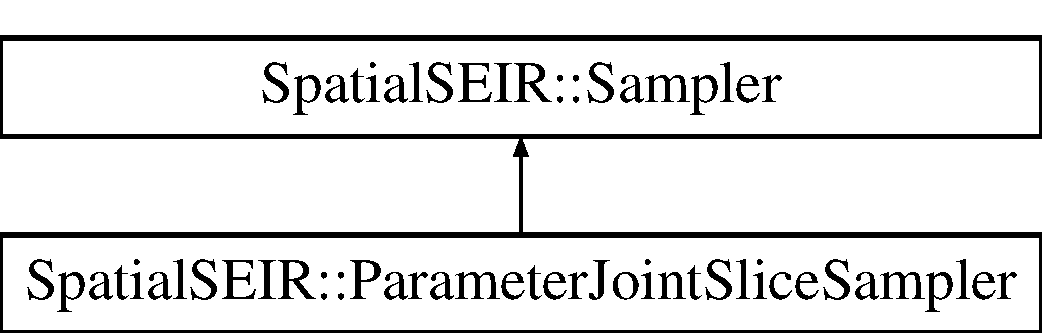
\includegraphics[height=2.000000cm]{classSpatialSEIR_1_1ParameterJointSliceSampler}
\end{center}
\end{figure}
\subsection*{Public Member Functions}
\begin{DoxyCompactItemize}
\item 
\hyperlink{classSpatialSEIR_1_1ParameterJointSliceSampler_af4a09549dbc8a2157f1e6879ecdbddf5}{Parameter\-Joint\-Slice\-Sampler} (\hyperlink{classSpatialSEIR_1_1ModelContext}{Model\-Context} $\ast$\hyperlink{classSpatialSEIR_1_1ParameterJointSliceSampler_adc70f8f5143b09aa830aa7b1c12c0853}{context}, \hyperlink{classSpatialSEIR_1_1ParameterFullConditional}{Parameter\-Full\-Conditional} $\ast$\hyperlink{classSpatialSEIR_1_1ParameterJointSliceSampler_a898ccd247b2ef346005ac437a600f4d4}{param\-F\-C}, double $\ast$\hyperlink{classSpatialSEIR_1_1ParameterJointSliceSampler_a405ce2949e75688013da196ecc139fa6}{param})
\item 
void \hyperlink{classSpatialSEIR_1_1ParameterJointSliceSampler_aceea42431db7eee7f58d4852cc8d1462}{draw\-Sample} ()
\item 
int \hyperlink{classSpatialSEIR_1_1ParameterJointSliceSampler_ac435f72bd91e0585b45d42233b0741dc}{get\-Sampler\-Type} ()
\item 
\hyperlink{classSpatialSEIR_1_1ParameterJointSliceSampler_a7c6303b5052965fce2460dc9f190b129}{$\sim$\-Parameter\-Joint\-Slice\-Sampler} ()
\end{DoxyCompactItemize}
\subsection*{Public Attributes}
\begin{DoxyCompactItemize}
\item 
double $\ast$$\ast$ \hyperlink{classSpatialSEIR_1_1ParameterJointSliceSampler_a405ce2949e75688013da196ecc139fa6}{param}
\item 
\hyperlink{classSpatialSEIR_1_1ModelContext}{Model\-Context} $\ast$$\ast$ \hyperlink{classSpatialSEIR_1_1ParameterJointSliceSampler_adc70f8f5143b09aa830aa7b1c12c0853}{context}
\item 
\hyperlink{classSpatialSEIR_1_1ParameterFullConditional}{Parameter\-Full\-Conditional} $\ast$$\ast$ \hyperlink{classSpatialSEIR_1_1ParameterJointSliceSampler_a898ccd247b2ef346005ac437a600f4d4}{param\-F\-C}
\end{DoxyCompactItemize}


\subsection{Detailed Description}
The \hyperlink{classSpatialSEIR_1_1ParameterJointSliceSampler}{Parameter\-Joint\-Slice\-Sampler} uses full vector slice sampling proposals to sample non Compartmental\-Matrix parameters. 

\subsection{Constructor \& Destructor Documentation}
\hypertarget{classSpatialSEIR_1_1ParameterJointSliceSampler_af4a09549dbc8a2157f1e6879ecdbddf5}{\index{Spatial\-S\-E\-I\-R\-::\-Parameter\-Joint\-Slice\-Sampler@{Spatial\-S\-E\-I\-R\-::\-Parameter\-Joint\-Slice\-Sampler}!Parameter\-Joint\-Slice\-Sampler@{Parameter\-Joint\-Slice\-Sampler}}
\index{Parameter\-Joint\-Slice\-Sampler@{Parameter\-Joint\-Slice\-Sampler}!SpatialSEIR::ParameterJointSliceSampler@{Spatial\-S\-E\-I\-R\-::\-Parameter\-Joint\-Slice\-Sampler}}
\subsubsection[{Parameter\-Joint\-Slice\-Sampler}]{\setlength{\rightskip}{0pt plus 5cm}Spatial\-S\-E\-I\-R\-::\-Parameter\-Joint\-Slice\-Sampler\-::\-Parameter\-Joint\-Slice\-Sampler (
\begin{DoxyParamCaption}
\item[{{\bf Model\-Context} $\ast$}]{context, }
\item[{{\bf Parameter\-Full\-Conditional} $\ast$}]{param\-F\-C, }
\item[{double $\ast$}]{param}
\end{DoxyParamCaption}
)}}\label{classSpatialSEIR_1_1ParameterJointSliceSampler_af4a09549dbc8a2157f1e6879ecdbddf5}
\hypertarget{classSpatialSEIR_1_1ParameterJointSliceSampler_a7c6303b5052965fce2460dc9f190b129}{\index{Spatial\-S\-E\-I\-R\-::\-Parameter\-Joint\-Slice\-Sampler@{Spatial\-S\-E\-I\-R\-::\-Parameter\-Joint\-Slice\-Sampler}!$\sim$\-Parameter\-Joint\-Slice\-Sampler@{$\sim$\-Parameter\-Joint\-Slice\-Sampler}}
\index{$\sim$\-Parameter\-Joint\-Slice\-Sampler@{$\sim$\-Parameter\-Joint\-Slice\-Sampler}!SpatialSEIR::ParameterJointSliceSampler@{Spatial\-S\-E\-I\-R\-::\-Parameter\-Joint\-Slice\-Sampler}}
\subsubsection[{$\sim$\-Parameter\-Joint\-Slice\-Sampler}]{\setlength{\rightskip}{0pt plus 5cm}Spatial\-S\-E\-I\-R\-::\-Parameter\-Joint\-Slice\-Sampler\-::$\sim$\-Parameter\-Joint\-Slice\-Sampler (
\begin{DoxyParamCaption}
{}
\end{DoxyParamCaption}
)}}\label{classSpatialSEIR_1_1ParameterJointSliceSampler_a7c6303b5052965fce2460dc9f190b129}


\subsection{Member Function Documentation}
\hypertarget{classSpatialSEIR_1_1ParameterJointSliceSampler_aceea42431db7eee7f58d4852cc8d1462}{\index{Spatial\-S\-E\-I\-R\-::\-Parameter\-Joint\-Slice\-Sampler@{Spatial\-S\-E\-I\-R\-::\-Parameter\-Joint\-Slice\-Sampler}!draw\-Sample@{draw\-Sample}}
\index{draw\-Sample@{draw\-Sample}!SpatialSEIR::ParameterJointSliceSampler@{Spatial\-S\-E\-I\-R\-::\-Parameter\-Joint\-Slice\-Sampler}}
\subsubsection[{draw\-Sample}]{\setlength{\rightskip}{0pt plus 5cm}void Spatial\-S\-E\-I\-R\-::\-Parameter\-Joint\-Slice\-Sampler\-::draw\-Sample (
\begin{DoxyParamCaption}
{}
\end{DoxyParamCaption}
)\hspace{0.3cm}{\ttfamily [virtual]}}}\label{classSpatialSEIR_1_1ParameterJointSliceSampler_aceea42431db7eee7f58d4852cc8d1462}


Implements \hyperlink{classSpatialSEIR_1_1Sampler_aa07a42b26cb62249c20c58e855a08657}{Spatial\-S\-E\-I\-R\-::\-Sampler}.

\hypertarget{classSpatialSEIR_1_1ParameterJointSliceSampler_ac435f72bd91e0585b45d42233b0741dc}{\index{Spatial\-S\-E\-I\-R\-::\-Parameter\-Joint\-Slice\-Sampler@{Spatial\-S\-E\-I\-R\-::\-Parameter\-Joint\-Slice\-Sampler}!get\-Sampler\-Type@{get\-Sampler\-Type}}
\index{get\-Sampler\-Type@{get\-Sampler\-Type}!SpatialSEIR::ParameterJointSliceSampler@{Spatial\-S\-E\-I\-R\-::\-Parameter\-Joint\-Slice\-Sampler}}
\subsubsection[{get\-Sampler\-Type}]{\setlength{\rightskip}{0pt plus 5cm}int Spatial\-S\-E\-I\-R\-::\-Parameter\-Joint\-Slice\-Sampler\-::get\-Sampler\-Type (
\begin{DoxyParamCaption}
{}
\end{DoxyParamCaption}
)\hspace{0.3cm}{\ttfamily [virtual]}}}\label{classSpatialSEIR_1_1ParameterJointSliceSampler_ac435f72bd91e0585b45d42233b0741dc}


Implements \hyperlink{classSpatialSEIR_1_1Sampler_aaa79310ad809e6aeb25479849f322dda}{Spatial\-S\-E\-I\-R\-::\-Sampler}.



\subsection{Member Data Documentation}
\hypertarget{classSpatialSEIR_1_1ParameterJointSliceSampler_adc70f8f5143b09aa830aa7b1c12c0853}{\index{Spatial\-S\-E\-I\-R\-::\-Parameter\-Joint\-Slice\-Sampler@{Spatial\-S\-E\-I\-R\-::\-Parameter\-Joint\-Slice\-Sampler}!context@{context}}
\index{context@{context}!SpatialSEIR::ParameterJointSliceSampler@{Spatial\-S\-E\-I\-R\-::\-Parameter\-Joint\-Slice\-Sampler}}
\subsubsection[{context}]{\setlength{\rightskip}{0pt plus 5cm}{\bf Model\-Context}$\ast$$\ast$ Spatial\-S\-E\-I\-R\-::\-Parameter\-Joint\-Slice\-Sampler\-::context}}\label{classSpatialSEIR_1_1ParameterJointSliceSampler_adc70f8f5143b09aa830aa7b1c12c0853}
\hypertarget{classSpatialSEIR_1_1ParameterJointSliceSampler_a405ce2949e75688013da196ecc139fa6}{\index{Spatial\-S\-E\-I\-R\-::\-Parameter\-Joint\-Slice\-Sampler@{Spatial\-S\-E\-I\-R\-::\-Parameter\-Joint\-Slice\-Sampler}!param@{param}}
\index{param@{param}!SpatialSEIR::ParameterJointSliceSampler@{Spatial\-S\-E\-I\-R\-::\-Parameter\-Joint\-Slice\-Sampler}}
\subsubsection[{param}]{\setlength{\rightskip}{0pt plus 5cm}double$\ast$$\ast$ Spatial\-S\-E\-I\-R\-::\-Parameter\-Joint\-Slice\-Sampler\-::param}}\label{classSpatialSEIR_1_1ParameterJointSliceSampler_a405ce2949e75688013da196ecc139fa6}
\hypertarget{classSpatialSEIR_1_1ParameterJointSliceSampler_a898ccd247b2ef346005ac437a600f4d4}{\index{Spatial\-S\-E\-I\-R\-::\-Parameter\-Joint\-Slice\-Sampler@{Spatial\-S\-E\-I\-R\-::\-Parameter\-Joint\-Slice\-Sampler}!param\-F\-C@{param\-F\-C}}
\index{param\-F\-C@{param\-F\-C}!SpatialSEIR::ParameterJointSliceSampler@{Spatial\-S\-E\-I\-R\-::\-Parameter\-Joint\-Slice\-Sampler}}
\subsubsection[{param\-F\-C}]{\setlength{\rightskip}{0pt plus 5cm}{\bf Parameter\-Full\-Conditional}$\ast$$\ast$ Spatial\-S\-E\-I\-R\-::\-Parameter\-Joint\-Slice\-Sampler\-::param\-F\-C}}\label{classSpatialSEIR_1_1ParameterJointSliceSampler_a898ccd247b2ef346005ac437a600f4d4}


The documentation for this class was generated from the following file\-:\begin{DoxyCompactItemize}
\item 
lib\-Spatial\-S\-E\-I\-R/include/\hyperlink{LSS__Samplers_8hpp}{L\-S\-S\-\_\-\-Samplers.\-hpp}\end{DoxyCompactItemize}

\hypertarget{classSpatialSEIR_1_1ParameterNullSampler}{\section{Spatial\-S\-E\-I\-R\-:\-:Parameter\-Null\-Sampler Class Reference}
\label{classSpatialSEIR_1_1ParameterNullSampler}\index{Spatial\-S\-E\-I\-R\-::\-Parameter\-Null\-Sampler@{Spatial\-S\-E\-I\-R\-::\-Parameter\-Null\-Sampler}}
}


{\ttfamily \#include $<$L\-S\-S\-\_\-\-Samplers.\-hpp$>$}

Inheritance diagram for Spatial\-S\-E\-I\-R\-:\-:Parameter\-Null\-Sampler\-:\begin{figure}[H]
\begin{center}
\leavevmode
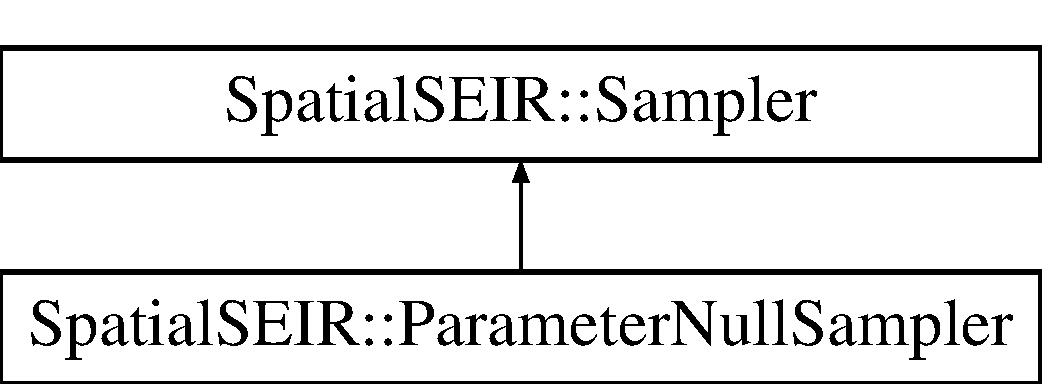
\includegraphics[height=2.000000cm]{classSpatialSEIR_1_1ParameterNullSampler}
\end{center}
\end{figure}
\subsection*{Additional Inherited Members}


\subsection{Detailed Description}
The \hyperlink{classSpatialSEIR_1_1ParameterNullSampler}{Parameter\-Null\-Sampler} class is a placeholder to prevent a full conditional distribution from updating. This is used if control has been handed to a \hyperlink{classSpatialSEIR_1_1ParameterHybridSampler}{Parameter\-Hybrid\-Sampler}. 

The documentation for this class was generated from the following file\-:\begin{DoxyCompactItemize}
\item 
lib\-Spatial\-S\-E\-I\-R/include/\hyperlink{LSS__Samplers_8hpp}{L\-S\-S\-\_\-\-Samplers.\-hpp}\end{DoxyCompactItemize}

\hypertarget{classSpatialSEIR_1_1ParameterSingleMetropolisSampler}{\section{Spatial\-S\-E\-I\-R\-:\-:Parameter\-Single\-Metropolis\-Sampler Class Reference}
\label{classSpatialSEIR_1_1ParameterSingleMetropolisSampler}\index{Spatial\-S\-E\-I\-R\-::\-Parameter\-Single\-Metropolis\-Sampler@{Spatial\-S\-E\-I\-R\-::\-Parameter\-Single\-Metropolis\-Sampler}}
}


{\ttfamily \#include $<$L\-S\-S\-\_\-\-Samplers.\-hpp$>$}

Inheritance diagram for Spatial\-S\-E\-I\-R\-:\-:Parameter\-Single\-Metropolis\-Sampler\-:\begin{figure}[H]
\begin{center}
\leavevmode
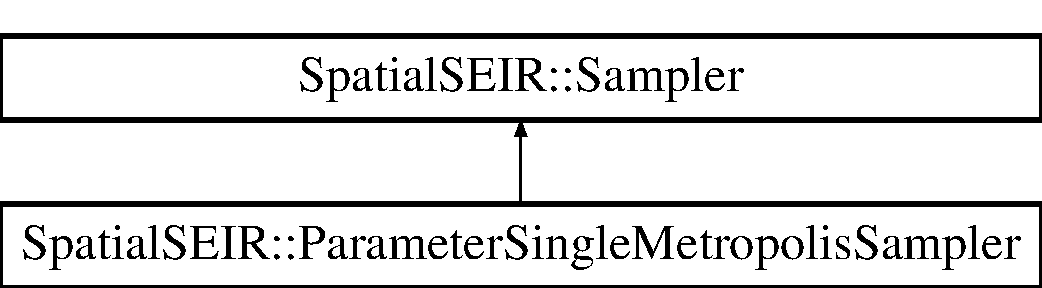
\includegraphics[height=2.000000cm]{classSpatialSEIR_1_1ParameterSingleMetropolisSampler}
\end{center}
\end{figure}
\subsection*{Public Member Functions}
\begin{DoxyCompactItemize}
\item 
\hyperlink{classSpatialSEIR_1_1ParameterSingleMetropolisSampler_a4918ba6b783bfabffa4fc42206a29ba3}{Parameter\-Single\-Metropolis\-Sampler} (\hyperlink{classSpatialSEIR_1_1ModelContext}{Model\-Context} $\ast$\hyperlink{classSpatialSEIR_1_1ParameterSingleMetropolisSampler_a4d66150fbe87614f62924200850ceb8d}{context}, \hyperlink{classSpatialSEIR_1_1ParameterFullConditional}{Parameter\-Full\-Conditional} $\ast$\hyperlink{classSpatialSEIR_1_1ParameterSingleMetropolisSampler_afa10a884a3c6772dfca224f058293dfd}{param\-F\-C}, double $\ast$\hyperlink{classSpatialSEIR_1_1ParameterSingleMetropolisSampler_a285f57aeb99f88605992bf25c9f38afb}{param})
\item 
void \hyperlink{classSpatialSEIR_1_1ParameterSingleMetropolisSampler_a637d48dfe689654490ab568e22e6037c}{draw\-Sample} ()
\item 
int \hyperlink{classSpatialSEIR_1_1ParameterSingleMetropolisSampler_a0576cfdda14e0afb0f63413f01a82c13}{get\-Sampler\-Type} ()
\item 
\hyperlink{classSpatialSEIR_1_1ParameterSingleMetropolisSampler_a3f55a283253add4cb4da09f2933275e3}{$\sim$\-Parameter\-Single\-Metropolis\-Sampler} ()
\end{DoxyCompactItemize}
\subsection*{Public Attributes}
\begin{DoxyCompactItemize}
\item 
double $\ast$$\ast$ \hyperlink{classSpatialSEIR_1_1ParameterSingleMetropolisSampler_a285f57aeb99f88605992bf25c9f38afb}{param}
\item 
\hyperlink{classSpatialSEIR_1_1ModelContext}{Model\-Context} $\ast$$\ast$ \hyperlink{classSpatialSEIR_1_1ParameterSingleMetropolisSampler_a4d66150fbe87614f62924200850ceb8d}{context}
\item 
\hyperlink{classSpatialSEIR_1_1ParameterFullConditional}{Parameter\-Full\-Conditional} $\ast$$\ast$ \hyperlink{classSpatialSEIR_1_1ParameterSingleMetropolisSampler_afa10a884a3c6772dfca224f058293dfd}{param\-F\-C}
\end{DoxyCompactItemize}


\subsection{Detailed Description}
The \hyperlink{classSpatialSEIR_1_1ParameterSingleMetropolisSampler}{Parameter\-Single\-Metropolis\-Sampler} uses Metropolis proposals of size one to sample non Compartmental\-Matrix parameters. 

\subsection{Constructor \& Destructor Documentation}
\hypertarget{classSpatialSEIR_1_1ParameterSingleMetropolisSampler_a4918ba6b783bfabffa4fc42206a29ba3}{\index{Spatial\-S\-E\-I\-R\-::\-Parameter\-Single\-Metropolis\-Sampler@{Spatial\-S\-E\-I\-R\-::\-Parameter\-Single\-Metropolis\-Sampler}!Parameter\-Single\-Metropolis\-Sampler@{Parameter\-Single\-Metropolis\-Sampler}}
\index{Parameter\-Single\-Metropolis\-Sampler@{Parameter\-Single\-Metropolis\-Sampler}!SpatialSEIR::ParameterSingleMetropolisSampler@{Spatial\-S\-E\-I\-R\-::\-Parameter\-Single\-Metropolis\-Sampler}}
\subsubsection[{Parameter\-Single\-Metropolis\-Sampler}]{\setlength{\rightskip}{0pt plus 5cm}Spatial\-S\-E\-I\-R\-::\-Parameter\-Single\-Metropolis\-Sampler\-::\-Parameter\-Single\-Metropolis\-Sampler (
\begin{DoxyParamCaption}
\item[{{\bf Model\-Context} $\ast$}]{context, }
\item[{{\bf Parameter\-Full\-Conditional} $\ast$}]{param\-F\-C, }
\item[{double $\ast$}]{param}
\end{DoxyParamCaption}
)}}\label{classSpatialSEIR_1_1ParameterSingleMetropolisSampler_a4918ba6b783bfabffa4fc42206a29ba3}
\hypertarget{classSpatialSEIR_1_1ParameterSingleMetropolisSampler_a3f55a283253add4cb4da09f2933275e3}{\index{Spatial\-S\-E\-I\-R\-::\-Parameter\-Single\-Metropolis\-Sampler@{Spatial\-S\-E\-I\-R\-::\-Parameter\-Single\-Metropolis\-Sampler}!$\sim$\-Parameter\-Single\-Metropolis\-Sampler@{$\sim$\-Parameter\-Single\-Metropolis\-Sampler}}
\index{$\sim$\-Parameter\-Single\-Metropolis\-Sampler@{$\sim$\-Parameter\-Single\-Metropolis\-Sampler}!SpatialSEIR::ParameterSingleMetropolisSampler@{Spatial\-S\-E\-I\-R\-::\-Parameter\-Single\-Metropolis\-Sampler}}
\subsubsection[{$\sim$\-Parameter\-Single\-Metropolis\-Sampler}]{\setlength{\rightskip}{0pt plus 5cm}Spatial\-S\-E\-I\-R\-::\-Parameter\-Single\-Metropolis\-Sampler\-::$\sim$\-Parameter\-Single\-Metropolis\-Sampler (
\begin{DoxyParamCaption}
{}
\end{DoxyParamCaption}
)}}\label{classSpatialSEIR_1_1ParameterSingleMetropolisSampler_a3f55a283253add4cb4da09f2933275e3}


\subsection{Member Function Documentation}
\hypertarget{classSpatialSEIR_1_1ParameterSingleMetropolisSampler_a637d48dfe689654490ab568e22e6037c}{\index{Spatial\-S\-E\-I\-R\-::\-Parameter\-Single\-Metropolis\-Sampler@{Spatial\-S\-E\-I\-R\-::\-Parameter\-Single\-Metropolis\-Sampler}!draw\-Sample@{draw\-Sample}}
\index{draw\-Sample@{draw\-Sample}!SpatialSEIR::ParameterSingleMetropolisSampler@{Spatial\-S\-E\-I\-R\-::\-Parameter\-Single\-Metropolis\-Sampler}}
\subsubsection[{draw\-Sample}]{\setlength{\rightskip}{0pt plus 5cm}void Spatial\-S\-E\-I\-R\-::\-Parameter\-Single\-Metropolis\-Sampler\-::draw\-Sample (
\begin{DoxyParamCaption}
{}
\end{DoxyParamCaption}
)\hspace{0.3cm}{\ttfamily [virtual]}}}\label{classSpatialSEIR_1_1ParameterSingleMetropolisSampler_a637d48dfe689654490ab568e22e6037c}


Implements \hyperlink{classSpatialSEIR_1_1Sampler_aa07a42b26cb62249c20c58e855a08657}{Spatial\-S\-E\-I\-R\-::\-Sampler}.

\hypertarget{classSpatialSEIR_1_1ParameterSingleMetropolisSampler_a0576cfdda14e0afb0f63413f01a82c13}{\index{Spatial\-S\-E\-I\-R\-::\-Parameter\-Single\-Metropolis\-Sampler@{Spatial\-S\-E\-I\-R\-::\-Parameter\-Single\-Metropolis\-Sampler}!get\-Sampler\-Type@{get\-Sampler\-Type}}
\index{get\-Sampler\-Type@{get\-Sampler\-Type}!SpatialSEIR::ParameterSingleMetropolisSampler@{Spatial\-S\-E\-I\-R\-::\-Parameter\-Single\-Metropolis\-Sampler}}
\subsubsection[{get\-Sampler\-Type}]{\setlength{\rightskip}{0pt plus 5cm}int Spatial\-S\-E\-I\-R\-::\-Parameter\-Single\-Metropolis\-Sampler\-::get\-Sampler\-Type (
\begin{DoxyParamCaption}
{}
\end{DoxyParamCaption}
)\hspace{0.3cm}{\ttfamily [virtual]}}}\label{classSpatialSEIR_1_1ParameterSingleMetropolisSampler_a0576cfdda14e0afb0f63413f01a82c13}


Implements \hyperlink{classSpatialSEIR_1_1Sampler_aaa79310ad809e6aeb25479849f322dda}{Spatial\-S\-E\-I\-R\-::\-Sampler}.



\subsection{Member Data Documentation}
\hypertarget{classSpatialSEIR_1_1ParameterSingleMetropolisSampler_a4d66150fbe87614f62924200850ceb8d}{\index{Spatial\-S\-E\-I\-R\-::\-Parameter\-Single\-Metropolis\-Sampler@{Spatial\-S\-E\-I\-R\-::\-Parameter\-Single\-Metropolis\-Sampler}!context@{context}}
\index{context@{context}!SpatialSEIR::ParameterSingleMetropolisSampler@{Spatial\-S\-E\-I\-R\-::\-Parameter\-Single\-Metropolis\-Sampler}}
\subsubsection[{context}]{\setlength{\rightskip}{0pt plus 5cm}{\bf Model\-Context}$\ast$$\ast$ Spatial\-S\-E\-I\-R\-::\-Parameter\-Single\-Metropolis\-Sampler\-::context}}\label{classSpatialSEIR_1_1ParameterSingleMetropolisSampler_a4d66150fbe87614f62924200850ceb8d}
\hypertarget{classSpatialSEIR_1_1ParameterSingleMetropolisSampler_a285f57aeb99f88605992bf25c9f38afb}{\index{Spatial\-S\-E\-I\-R\-::\-Parameter\-Single\-Metropolis\-Sampler@{Spatial\-S\-E\-I\-R\-::\-Parameter\-Single\-Metropolis\-Sampler}!param@{param}}
\index{param@{param}!SpatialSEIR::ParameterSingleMetropolisSampler@{Spatial\-S\-E\-I\-R\-::\-Parameter\-Single\-Metropolis\-Sampler}}
\subsubsection[{param}]{\setlength{\rightskip}{0pt plus 5cm}double$\ast$$\ast$ Spatial\-S\-E\-I\-R\-::\-Parameter\-Single\-Metropolis\-Sampler\-::param}}\label{classSpatialSEIR_1_1ParameterSingleMetropolisSampler_a285f57aeb99f88605992bf25c9f38afb}
\hypertarget{classSpatialSEIR_1_1ParameterSingleMetropolisSampler_afa10a884a3c6772dfca224f058293dfd}{\index{Spatial\-S\-E\-I\-R\-::\-Parameter\-Single\-Metropolis\-Sampler@{Spatial\-S\-E\-I\-R\-::\-Parameter\-Single\-Metropolis\-Sampler}!param\-F\-C@{param\-F\-C}}
\index{param\-F\-C@{param\-F\-C}!SpatialSEIR::ParameterSingleMetropolisSampler@{Spatial\-S\-E\-I\-R\-::\-Parameter\-Single\-Metropolis\-Sampler}}
\subsubsection[{param\-F\-C}]{\setlength{\rightskip}{0pt plus 5cm}{\bf Parameter\-Full\-Conditional}$\ast$$\ast$ Spatial\-S\-E\-I\-R\-::\-Parameter\-Single\-Metropolis\-Sampler\-::param\-F\-C}}\label{classSpatialSEIR_1_1ParameterSingleMetropolisSampler_afa10a884a3c6772dfca224f058293dfd}


The documentation for this class was generated from the following file\-:\begin{DoxyCompactItemize}
\item 
lib\-Spatial\-S\-E\-I\-R/include/\hyperlink{LSS__Samplers_8hpp}{L\-S\-S\-\_\-\-Samplers.\-hpp}\end{DoxyCompactItemize}

\hypertarget{classSpatialSEIR_1_1PerformDecorrelationStep}{\section{Spatial\-S\-E\-I\-R\-:\-:Perform\-Decorrelation\-Step Class Reference}
\label{classSpatialSEIR_1_1PerformDecorrelationStep}\index{Spatial\-S\-E\-I\-R\-::\-Perform\-Decorrelation\-Step@{Spatial\-S\-E\-I\-R\-::\-Perform\-Decorrelation\-Step}}
}


{\ttfamily \#include $<$L\-S\-S\-\_\-\-Iteration\-Tasks.\-hpp$>$}

Inheritance diagram for Spatial\-S\-E\-I\-R\-:\-:Perform\-Decorrelation\-Step\-:\begin{figure}[H]
\begin{center}
\leavevmode
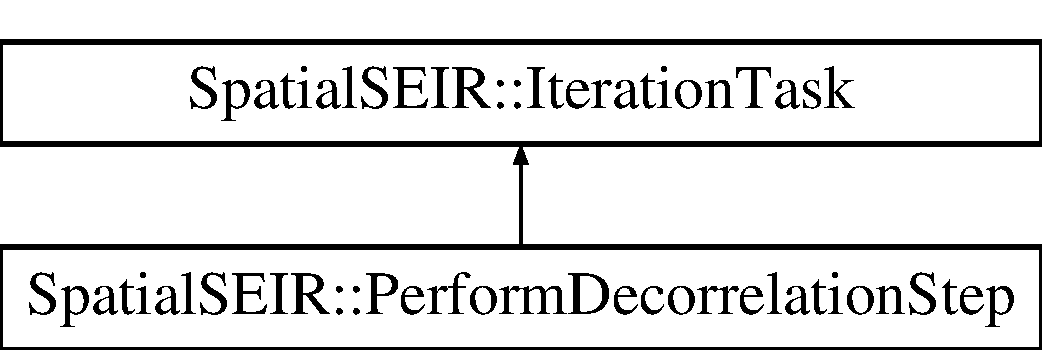
\includegraphics[height=2.000000cm]{classSpatialSEIR_1_1PerformDecorrelationStep}
\end{center}
\end{figure}
\subsection*{Public Member Functions}
\begin{DoxyCompactItemize}
\item 
\hyperlink{classSpatialSEIR_1_1PerformDecorrelationStep_ae78265340fd46d9ff674ca7d6cbc86bf}{Perform\-Decorrelation\-Step} (\hyperlink{classSpatialSEIR_1_1ModelContext}{Model\-Context} $\ast$\hyperlink{classSpatialSEIR_1_1PerformDecorrelationStep_ad02138912341efd070e7f38a6743f014}{context}, int \hyperlink{classSpatialSEIR_1_1PerformDecorrelationStep_a78eb6b88ca3e77d7cb482ad30bbfa552}{iteration\-Count})
\item 
\hyperlink{classSpatialSEIR_1_1PerformDecorrelationStep_a9fe8a9b0a0b852f3bd83fb8ad4a2e3e6}{$\sim$\-Perform\-Decorrelation\-Step} ()
\item 
void \hyperlink{classSpatialSEIR_1_1PerformDecorrelationStep_a62dcdeaf7c8ce7482981c94570600363}{execute\-Task} ()
\item 
int \hyperlink{classSpatialSEIR_1_1PerformDecorrelationStep_a04fcb1e5d1c16ae563c034ea30467cc7}{get\-Task\-Type} ()
\end{DoxyCompactItemize}
\subsection*{Public Attributes}
\begin{DoxyCompactItemize}
\item 
\hyperlink{classSpatialSEIR_1_1ModelContext}{Model\-Context} $\ast$$\ast$ \hyperlink{classSpatialSEIR_1_1PerformDecorrelationStep_ad02138912341efd070e7f38a6743f014}{context}
\item 
int $\ast$ \hyperlink{classSpatialSEIR_1_1PerformDecorrelationStep_a78eb6b88ca3e77d7cb482ad30bbfa552}{iteration\-Count}
\item 
int $\ast$ \hyperlink{classSpatialSEIR_1_1PerformDecorrelationStep_aeb81e294b08d0665e22b5c92e94075de}{current\-Iteration}
\end{DoxyCompactItemize}


\subsection{Constructor \& Destructor Documentation}
\hypertarget{classSpatialSEIR_1_1PerformDecorrelationStep_ae78265340fd46d9ff674ca7d6cbc86bf}{\index{Spatial\-S\-E\-I\-R\-::\-Perform\-Decorrelation\-Step@{Spatial\-S\-E\-I\-R\-::\-Perform\-Decorrelation\-Step}!Perform\-Decorrelation\-Step@{Perform\-Decorrelation\-Step}}
\index{Perform\-Decorrelation\-Step@{Perform\-Decorrelation\-Step}!SpatialSEIR::PerformDecorrelationStep@{Spatial\-S\-E\-I\-R\-::\-Perform\-Decorrelation\-Step}}
\subsubsection[{Perform\-Decorrelation\-Step}]{\setlength{\rightskip}{0pt plus 5cm}Spatial\-S\-E\-I\-R\-::\-Perform\-Decorrelation\-Step\-::\-Perform\-Decorrelation\-Step (
\begin{DoxyParamCaption}
\item[{{\bf Model\-Context} $\ast$}]{context, }
\item[{int}]{iteration\-Count}
\end{DoxyParamCaption}
)}}\label{classSpatialSEIR_1_1PerformDecorrelationStep_ae78265340fd46d9ff674ca7d6cbc86bf}
\hypertarget{classSpatialSEIR_1_1PerformDecorrelationStep_a9fe8a9b0a0b852f3bd83fb8ad4a2e3e6}{\index{Spatial\-S\-E\-I\-R\-::\-Perform\-Decorrelation\-Step@{Spatial\-S\-E\-I\-R\-::\-Perform\-Decorrelation\-Step}!$\sim$\-Perform\-Decorrelation\-Step@{$\sim$\-Perform\-Decorrelation\-Step}}
\index{$\sim$\-Perform\-Decorrelation\-Step@{$\sim$\-Perform\-Decorrelation\-Step}!SpatialSEIR::PerformDecorrelationStep@{Spatial\-S\-E\-I\-R\-::\-Perform\-Decorrelation\-Step}}
\subsubsection[{$\sim$\-Perform\-Decorrelation\-Step}]{\setlength{\rightskip}{0pt plus 5cm}Spatial\-S\-E\-I\-R\-::\-Perform\-Decorrelation\-Step\-::$\sim$\-Perform\-Decorrelation\-Step (
\begin{DoxyParamCaption}
{}
\end{DoxyParamCaption}
)}}\label{classSpatialSEIR_1_1PerformDecorrelationStep_a9fe8a9b0a0b852f3bd83fb8ad4a2e3e6}


\subsection{Member Function Documentation}
\hypertarget{classSpatialSEIR_1_1PerformDecorrelationStep_a62dcdeaf7c8ce7482981c94570600363}{\index{Spatial\-S\-E\-I\-R\-::\-Perform\-Decorrelation\-Step@{Spatial\-S\-E\-I\-R\-::\-Perform\-Decorrelation\-Step}!execute\-Task@{execute\-Task}}
\index{execute\-Task@{execute\-Task}!SpatialSEIR::PerformDecorrelationStep@{Spatial\-S\-E\-I\-R\-::\-Perform\-Decorrelation\-Step}}
\subsubsection[{execute\-Task}]{\setlength{\rightskip}{0pt plus 5cm}void Spatial\-S\-E\-I\-R\-::\-Perform\-Decorrelation\-Step\-::execute\-Task (
\begin{DoxyParamCaption}
{}
\end{DoxyParamCaption}
)\hspace{0.3cm}{\ttfamily [virtual]}}}\label{classSpatialSEIR_1_1PerformDecorrelationStep_a62dcdeaf7c8ce7482981c94570600363}


Implements \hyperlink{classSpatialSEIR_1_1IterationTask_a68fcb08fe777ed506c97dc1ac5a0fb54}{Spatial\-S\-E\-I\-R\-::\-Iteration\-Task}.

\hypertarget{classSpatialSEIR_1_1PerformDecorrelationStep_a04fcb1e5d1c16ae563c034ea30467cc7}{\index{Spatial\-S\-E\-I\-R\-::\-Perform\-Decorrelation\-Step@{Spatial\-S\-E\-I\-R\-::\-Perform\-Decorrelation\-Step}!get\-Task\-Type@{get\-Task\-Type}}
\index{get\-Task\-Type@{get\-Task\-Type}!SpatialSEIR::PerformDecorrelationStep@{Spatial\-S\-E\-I\-R\-::\-Perform\-Decorrelation\-Step}}
\subsubsection[{get\-Task\-Type}]{\setlength{\rightskip}{0pt plus 5cm}int Spatial\-S\-E\-I\-R\-::\-Perform\-Decorrelation\-Step\-::get\-Task\-Type (
\begin{DoxyParamCaption}
{}
\end{DoxyParamCaption}
)\hspace{0.3cm}{\ttfamily [virtual]}}}\label{classSpatialSEIR_1_1PerformDecorrelationStep_a04fcb1e5d1c16ae563c034ea30467cc7}


Implements \hyperlink{classSpatialSEIR_1_1IterationTask_aaba9c737c4564df6b44b843d7c781722}{Spatial\-S\-E\-I\-R\-::\-Iteration\-Task}.



\subsection{Member Data Documentation}
\hypertarget{classSpatialSEIR_1_1PerformDecorrelationStep_ad02138912341efd070e7f38a6743f014}{\index{Spatial\-S\-E\-I\-R\-::\-Perform\-Decorrelation\-Step@{Spatial\-S\-E\-I\-R\-::\-Perform\-Decorrelation\-Step}!context@{context}}
\index{context@{context}!SpatialSEIR::PerformDecorrelationStep@{Spatial\-S\-E\-I\-R\-::\-Perform\-Decorrelation\-Step}}
\subsubsection[{context}]{\setlength{\rightskip}{0pt plus 5cm}{\bf Model\-Context}$\ast$$\ast$ Spatial\-S\-E\-I\-R\-::\-Perform\-Decorrelation\-Step\-::context}}\label{classSpatialSEIR_1_1PerformDecorrelationStep_ad02138912341efd070e7f38a6743f014}
\hypertarget{classSpatialSEIR_1_1PerformDecorrelationStep_aeb81e294b08d0665e22b5c92e94075de}{\index{Spatial\-S\-E\-I\-R\-::\-Perform\-Decorrelation\-Step@{Spatial\-S\-E\-I\-R\-::\-Perform\-Decorrelation\-Step}!current\-Iteration@{current\-Iteration}}
\index{current\-Iteration@{current\-Iteration}!SpatialSEIR::PerformDecorrelationStep@{Spatial\-S\-E\-I\-R\-::\-Perform\-Decorrelation\-Step}}
\subsubsection[{current\-Iteration}]{\setlength{\rightskip}{0pt plus 5cm}int$\ast$ Spatial\-S\-E\-I\-R\-::\-Perform\-Decorrelation\-Step\-::current\-Iteration}}\label{classSpatialSEIR_1_1PerformDecorrelationStep_aeb81e294b08d0665e22b5c92e94075de}
\hypertarget{classSpatialSEIR_1_1PerformDecorrelationStep_a78eb6b88ca3e77d7cb482ad30bbfa552}{\index{Spatial\-S\-E\-I\-R\-::\-Perform\-Decorrelation\-Step@{Spatial\-S\-E\-I\-R\-::\-Perform\-Decorrelation\-Step}!iteration\-Count@{iteration\-Count}}
\index{iteration\-Count@{iteration\-Count}!SpatialSEIR::PerformDecorrelationStep@{Spatial\-S\-E\-I\-R\-::\-Perform\-Decorrelation\-Step}}
\subsubsection[{iteration\-Count}]{\setlength{\rightskip}{0pt plus 5cm}int$\ast$ Spatial\-S\-E\-I\-R\-::\-Perform\-Decorrelation\-Step\-::iteration\-Count}}\label{classSpatialSEIR_1_1PerformDecorrelationStep_a78eb6b88ca3e77d7cb482ad30bbfa552}


The documentation for this class was generated from the following file\-:\begin{DoxyCompactItemize}
\item 
lib\-Spatial\-S\-E\-I\-R/include/\hyperlink{LSS__IterationTasks_8hpp}{L\-S\-S\-\_\-\-Iteration\-Tasks.\-hpp}\end{DoxyCompactItemize}

\hypertarget{classSpatialSEIR_1_1PerformHybridSE__EI__UpdateStep}{\section{Spatial\-S\-E\-I\-R\-:\-:Perform\-Hybrid\-S\-E\-\_\-\-E\-I\-\_\-\-Update\-Step Class Reference}
\label{classSpatialSEIR_1_1PerformHybridSE__EI__UpdateStep}\index{Spatial\-S\-E\-I\-R\-::\-Perform\-Hybrid\-S\-E\-\_\-\-E\-I\-\_\-\-Update\-Step@{Spatial\-S\-E\-I\-R\-::\-Perform\-Hybrid\-S\-E\-\_\-\-E\-I\-\_\-\-Update\-Step}}
}


{\ttfamily \#include $<$L\-S\-S\-\_\-\-Iteration\-Tasks.\-hpp$>$}

Inheritance diagram for Spatial\-S\-E\-I\-R\-:\-:Perform\-Hybrid\-S\-E\-\_\-\-E\-I\-\_\-\-Update\-Step\-:\begin{figure}[H]
\begin{center}
\leavevmode
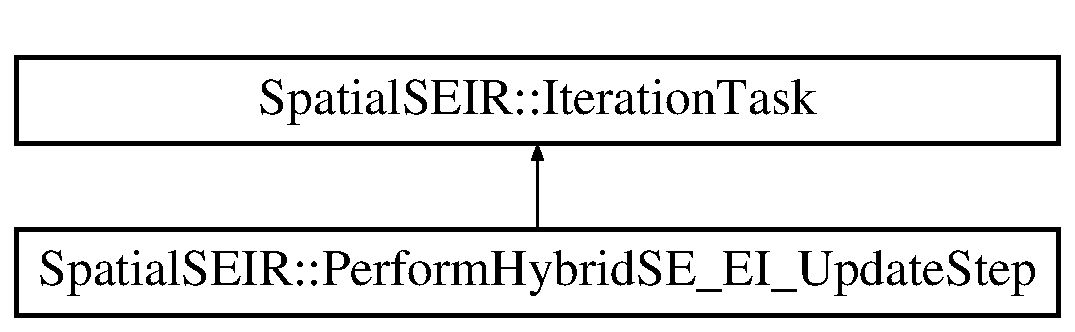
\includegraphics[height=2.000000cm]{classSpatialSEIR_1_1PerformHybridSE__EI__UpdateStep}
\end{center}
\end{figure}
\subsection*{Public Member Functions}
\begin{DoxyCompactItemize}
\item 
\hyperlink{classSpatialSEIR_1_1PerformHybridSE__EI__UpdateStep_a4916ca2382b89ba23441da1c51715d59}{Perform\-Hybrid\-S\-E\-\_\-\-E\-I\-\_\-\-Update\-Step} (\hyperlink{classSpatialSEIR_1_1ModelContext}{Model\-Context} $\ast$\hyperlink{classSpatialSEIR_1_1PerformHybridSE__EI__UpdateStep_a94eb8f51d2429aab817816ce7ebaf511}{context}, \hyperlink{classSpatialSEIR_1_1FC__Gamma__EI}{F\-C\-\_\-\-Gamma\-\_\-\-E\-I} $\ast$fc\-\_\-gamma\-E\-I, \hyperlink{classSpatialSEIR_1_1FC__Beta}{F\-C\-\_\-\-Beta} $\ast$fc\-\_\-beta, int \hyperlink{classSpatialSEIR_1_1PerformHybridSE__EI__UpdateStep_adba72b268c525551ffd68721cfe766e1}{iteration\-Count})
\item 
\hyperlink{classSpatialSEIR_1_1PerformHybridSE__EI__UpdateStep_a0c6d29ffa4d6e6e755a0e000140fdbcf}{$\sim$\-Perform\-Hybrid\-S\-E\-\_\-\-E\-I\-\_\-\-Update\-Step} ()
\item 
void \hyperlink{classSpatialSEIR_1_1PerformHybridSE__EI__UpdateStep_af4f28e1f994de584711e2878eb60afe3}{execute\-Task} ()
\item 
int \hyperlink{classSpatialSEIR_1_1PerformHybridSE__EI__UpdateStep_adc6e6e6e9c1121b3d5a38910d7f2731e}{get\-Task\-Type} ()
\end{DoxyCompactItemize}
\subsection*{Public Attributes}
\begin{DoxyCompactItemize}
\item 
\hyperlink{classSpatialSEIR_1_1ModelContext}{Model\-Context} $\ast$$\ast$ \hyperlink{classSpatialSEIR_1_1PerformHybridSE__EI__UpdateStep_a94eb8f51d2429aab817816ce7ebaf511}{context}
\item 
\hyperlink{classSpatialSEIR_1_1ParameterHybridSampler}{Parameter\-Hybrid\-Sampler} $\ast$ \hyperlink{classSpatialSEIR_1_1PerformHybridSE__EI__UpdateStep_a9afc7c610b2be704bc1517ce8b566534}{sampler}
\item 
int $\ast$ \hyperlink{classSpatialSEIR_1_1PerformHybridSE__EI__UpdateStep_adba72b268c525551ffd68721cfe766e1}{iteration\-Count}
\item 
int $\ast$ \hyperlink{classSpatialSEIR_1_1PerformHybridSE__EI__UpdateStep_a0e09a6ce9b5dad69515d3eb42367b525}{current\-Iteration}
\end{DoxyCompactItemize}


\subsection{Constructor \& Destructor Documentation}
\hypertarget{classSpatialSEIR_1_1PerformHybridSE__EI__UpdateStep_a4916ca2382b89ba23441da1c51715d59}{\index{Spatial\-S\-E\-I\-R\-::\-Perform\-Hybrid\-S\-E\-\_\-\-E\-I\-\_\-\-Update\-Step@{Spatial\-S\-E\-I\-R\-::\-Perform\-Hybrid\-S\-E\-\_\-\-E\-I\-\_\-\-Update\-Step}!Perform\-Hybrid\-S\-E\-\_\-\-E\-I\-\_\-\-Update\-Step@{Perform\-Hybrid\-S\-E\-\_\-\-E\-I\-\_\-\-Update\-Step}}
\index{Perform\-Hybrid\-S\-E\-\_\-\-E\-I\-\_\-\-Update\-Step@{Perform\-Hybrid\-S\-E\-\_\-\-E\-I\-\_\-\-Update\-Step}!SpatialSEIR::PerformHybridSE_EI_UpdateStep@{Spatial\-S\-E\-I\-R\-::\-Perform\-Hybrid\-S\-E\-\_\-\-E\-I\-\_\-\-Update\-Step}}
\subsubsection[{Perform\-Hybrid\-S\-E\-\_\-\-E\-I\-\_\-\-Update\-Step}]{\setlength{\rightskip}{0pt plus 5cm}Spatial\-S\-E\-I\-R\-::\-Perform\-Hybrid\-S\-E\-\_\-\-E\-I\-\_\-\-Update\-Step\-::\-Perform\-Hybrid\-S\-E\-\_\-\-E\-I\-\_\-\-Update\-Step (
\begin{DoxyParamCaption}
\item[{{\bf Model\-Context} $\ast$}]{context, }
\item[{{\bf F\-C\-\_\-\-Gamma\-\_\-\-E\-I} $\ast$}]{fc\-\_\-gamma\-E\-I, }
\item[{{\bf F\-C\-\_\-\-Beta} $\ast$}]{fc\-\_\-beta, }
\item[{int}]{iteration\-Count}
\end{DoxyParamCaption}
)}}\label{classSpatialSEIR_1_1PerformHybridSE__EI__UpdateStep_a4916ca2382b89ba23441da1c51715d59}
\hypertarget{classSpatialSEIR_1_1PerformHybridSE__EI__UpdateStep_a0c6d29ffa4d6e6e755a0e000140fdbcf}{\index{Spatial\-S\-E\-I\-R\-::\-Perform\-Hybrid\-S\-E\-\_\-\-E\-I\-\_\-\-Update\-Step@{Spatial\-S\-E\-I\-R\-::\-Perform\-Hybrid\-S\-E\-\_\-\-E\-I\-\_\-\-Update\-Step}!$\sim$\-Perform\-Hybrid\-S\-E\-\_\-\-E\-I\-\_\-\-Update\-Step@{$\sim$\-Perform\-Hybrid\-S\-E\-\_\-\-E\-I\-\_\-\-Update\-Step}}
\index{$\sim$\-Perform\-Hybrid\-S\-E\-\_\-\-E\-I\-\_\-\-Update\-Step@{$\sim$\-Perform\-Hybrid\-S\-E\-\_\-\-E\-I\-\_\-\-Update\-Step}!SpatialSEIR::PerformHybridSE_EI_UpdateStep@{Spatial\-S\-E\-I\-R\-::\-Perform\-Hybrid\-S\-E\-\_\-\-E\-I\-\_\-\-Update\-Step}}
\subsubsection[{$\sim$\-Perform\-Hybrid\-S\-E\-\_\-\-E\-I\-\_\-\-Update\-Step}]{\setlength{\rightskip}{0pt plus 5cm}Spatial\-S\-E\-I\-R\-::\-Perform\-Hybrid\-S\-E\-\_\-\-E\-I\-\_\-\-Update\-Step\-::$\sim$\-Perform\-Hybrid\-S\-E\-\_\-\-E\-I\-\_\-\-Update\-Step (
\begin{DoxyParamCaption}
{}
\end{DoxyParamCaption}
)}}\label{classSpatialSEIR_1_1PerformHybridSE__EI__UpdateStep_a0c6d29ffa4d6e6e755a0e000140fdbcf}


\subsection{Member Function Documentation}
\hypertarget{classSpatialSEIR_1_1PerformHybridSE__EI__UpdateStep_af4f28e1f994de584711e2878eb60afe3}{\index{Spatial\-S\-E\-I\-R\-::\-Perform\-Hybrid\-S\-E\-\_\-\-E\-I\-\_\-\-Update\-Step@{Spatial\-S\-E\-I\-R\-::\-Perform\-Hybrid\-S\-E\-\_\-\-E\-I\-\_\-\-Update\-Step}!execute\-Task@{execute\-Task}}
\index{execute\-Task@{execute\-Task}!SpatialSEIR::PerformHybridSE_EI_UpdateStep@{Spatial\-S\-E\-I\-R\-::\-Perform\-Hybrid\-S\-E\-\_\-\-E\-I\-\_\-\-Update\-Step}}
\subsubsection[{execute\-Task}]{\setlength{\rightskip}{0pt plus 5cm}void Spatial\-S\-E\-I\-R\-::\-Perform\-Hybrid\-S\-E\-\_\-\-E\-I\-\_\-\-Update\-Step\-::execute\-Task (
\begin{DoxyParamCaption}
{}
\end{DoxyParamCaption}
)\hspace{0.3cm}{\ttfamily [virtual]}}}\label{classSpatialSEIR_1_1PerformHybridSE__EI__UpdateStep_af4f28e1f994de584711e2878eb60afe3}


Implements \hyperlink{classSpatialSEIR_1_1IterationTask_a68fcb08fe777ed506c97dc1ac5a0fb54}{Spatial\-S\-E\-I\-R\-::\-Iteration\-Task}.

\hypertarget{classSpatialSEIR_1_1PerformHybridSE__EI__UpdateStep_adc6e6e6e9c1121b3d5a38910d7f2731e}{\index{Spatial\-S\-E\-I\-R\-::\-Perform\-Hybrid\-S\-E\-\_\-\-E\-I\-\_\-\-Update\-Step@{Spatial\-S\-E\-I\-R\-::\-Perform\-Hybrid\-S\-E\-\_\-\-E\-I\-\_\-\-Update\-Step}!get\-Task\-Type@{get\-Task\-Type}}
\index{get\-Task\-Type@{get\-Task\-Type}!SpatialSEIR::PerformHybridSE_EI_UpdateStep@{Spatial\-S\-E\-I\-R\-::\-Perform\-Hybrid\-S\-E\-\_\-\-E\-I\-\_\-\-Update\-Step}}
\subsubsection[{get\-Task\-Type}]{\setlength{\rightskip}{0pt plus 5cm}int Spatial\-S\-E\-I\-R\-::\-Perform\-Hybrid\-S\-E\-\_\-\-E\-I\-\_\-\-Update\-Step\-::get\-Task\-Type (
\begin{DoxyParamCaption}
{}
\end{DoxyParamCaption}
)\hspace{0.3cm}{\ttfamily [virtual]}}}\label{classSpatialSEIR_1_1PerformHybridSE__EI__UpdateStep_adc6e6e6e9c1121b3d5a38910d7f2731e}


Implements \hyperlink{classSpatialSEIR_1_1IterationTask_aaba9c737c4564df6b44b843d7c781722}{Spatial\-S\-E\-I\-R\-::\-Iteration\-Task}.



\subsection{Member Data Documentation}
\hypertarget{classSpatialSEIR_1_1PerformHybridSE__EI__UpdateStep_a94eb8f51d2429aab817816ce7ebaf511}{\index{Spatial\-S\-E\-I\-R\-::\-Perform\-Hybrid\-S\-E\-\_\-\-E\-I\-\_\-\-Update\-Step@{Spatial\-S\-E\-I\-R\-::\-Perform\-Hybrid\-S\-E\-\_\-\-E\-I\-\_\-\-Update\-Step}!context@{context}}
\index{context@{context}!SpatialSEIR::PerformHybridSE_EI_UpdateStep@{Spatial\-S\-E\-I\-R\-::\-Perform\-Hybrid\-S\-E\-\_\-\-E\-I\-\_\-\-Update\-Step}}
\subsubsection[{context}]{\setlength{\rightskip}{0pt plus 5cm}{\bf Model\-Context}$\ast$$\ast$ Spatial\-S\-E\-I\-R\-::\-Perform\-Hybrid\-S\-E\-\_\-\-E\-I\-\_\-\-Update\-Step\-::context}}\label{classSpatialSEIR_1_1PerformHybridSE__EI__UpdateStep_a94eb8f51d2429aab817816ce7ebaf511}
\hypertarget{classSpatialSEIR_1_1PerformHybridSE__EI__UpdateStep_a0e09a6ce9b5dad69515d3eb42367b525}{\index{Spatial\-S\-E\-I\-R\-::\-Perform\-Hybrid\-S\-E\-\_\-\-E\-I\-\_\-\-Update\-Step@{Spatial\-S\-E\-I\-R\-::\-Perform\-Hybrid\-S\-E\-\_\-\-E\-I\-\_\-\-Update\-Step}!current\-Iteration@{current\-Iteration}}
\index{current\-Iteration@{current\-Iteration}!SpatialSEIR::PerformHybridSE_EI_UpdateStep@{Spatial\-S\-E\-I\-R\-::\-Perform\-Hybrid\-S\-E\-\_\-\-E\-I\-\_\-\-Update\-Step}}
\subsubsection[{current\-Iteration}]{\setlength{\rightskip}{0pt plus 5cm}int$\ast$ Spatial\-S\-E\-I\-R\-::\-Perform\-Hybrid\-S\-E\-\_\-\-E\-I\-\_\-\-Update\-Step\-::current\-Iteration}}\label{classSpatialSEIR_1_1PerformHybridSE__EI__UpdateStep_a0e09a6ce9b5dad69515d3eb42367b525}
\hypertarget{classSpatialSEIR_1_1PerformHybridSE__EI__UpdateStep_adba72b268c525551ffd68721cfe766e1}{\index{Spatial\-S\-E\-I\-R\-::\-Perform\-Hybrid\-S\-E\-\_\-\-E\-I\-\_\-\-Update\-Step@{Spatial\-S\-E\-I\-R\-::\-Perform\-Hybrid\-S\-E\-\_\-\-E\-I\-\_\-\-Update\-Step}!iteration\-Count@{iteration\-Count}}
\index{iteration\-Count@{iteration\-Count}!SpatialSEIR::PerformHybridSE_EI_UpdateStep@{Spatial\-S\-E\-I\-R\-::\-Perform\-Hybrid\-S\-E\-\_\-\-E\-I\-\_\-\-Update\-Step}}
\subsubsection[{iteration\-Count}]{\setlength{\rightskip}{0pt plus 5cm}int$\ast$ Spatial\-S\-E\-I\-R\-::\-Perform\-Hybrid\-S\-E\-\_\-\-E\-I\-\_\-\-Update\-Step\-::iteration\-Count}}\label{classSpatialSEIR_1_1PerformHybridSE__EI__UpdateStep_adba72b268c525551ffd68721cfe766e1}
\hypertarget{classSpatialSEIR_1_1PerformHybridSE__EI__UpdateStep_a9afc7c610b2be704bc1517ce8b566534}{\index{Spatial\-S\-E\-I\-R\-::\-Perform\-Hybrid\-S\-E\-\_\-\-E\-I\-\_\-\-Update\-Step@{Spatial\-S\-E\-I\-R\-::\-Perform\-Hybrid\-S\-E\-\_\-\-E\-I\-\_\-\-Update\-Step}!sampler@{sampler}}
\index{sampler@{sampler}!SpatialSEIR::PerformHybridSE_EI_UpdateStep@{Spatial\-S\-E\-I\-R\-::\-Perform\-Hybrid\-S\-E\-\_\-\-E\-I\-\_\-\-Update\-Step}}
\subsubsection[{sampler}]{\setlength{\rightskip}{0pt plus 5cm}{\bf Parameter\-Hybrid\-Sampler}$\ast$ Spatial\-S\-E\-I\-R\-::\-Perform\-Hybrid\-S\-E\-\_\-\-E\-I\-\_\-\-Update\-Step\-::sampler}}\label{classSpatialSEIR_1_1PerformHybridSE__EI__UpdateStep_a9afc7c610b2be704bc1517ce8b566534}


The documentation for this class was generated from the following file\-:\begin{DoxyCompactItemize}
\item 
lib\-Spatial\-S\-E\-I\-R/include/\hyperlink{LSS__IterationTasks_8hpp}{L\-S\-S\-\_\-\-Iteration\-Tasks.\-hpp}\end{DoxyCompactItemize}

\hypertarget{structSpatialSEIR_1_1priorControl}{\section{Spatial\-S\-E\-I\-R\-:\-:prior\-Control Struct Reference}
\label{structSpatialSEIR_1_1priorControl}\index{Spatial\-S\-E\-I\-R\-::prior\-Control@{Spatial\-S\-E\-I\-R\-::prior\-Control}}
}


struct containing hyperparameters for beta, beta\-P\-\_\-\-R\-S, P\-\_\-\-E\-I, and P\-\_\-\-I\-R  




{\ttfamily \#include $<$L\-S\-S\-\_\-\-Full\-Conditional.\-hpp$>$}

\subsection*{Public Attributes}
\begin{DoxyCompactItemize}
\item 
double \hyperlink{structSpatialSEIR_1_1priorControl_a09b61ec7e9aeffb5240b2deb91c2caa7}{beta\-Prior\-Precision}
\item 
double \hyperlink{structSpatialSEIR_1_1priorControl_a217fafa2c871f52851ddf117fa102a99}{beta\-Prs\-Prior\-Precision}
\item 
double \hyperlink{structSpatialSEIR_1_1priorControl_a480e374c2292f8c4ec4001b9200d3c98}{P\-\_\-\-E\-I\-\_\-prior\-Alpha}
\item 
double \hyperlink{structSpatialSEIR_1_1priorControl_a03121f3205c6a9ad8b9eba19bc2d984a}{P\-\_\-\-E\-I\-\_\-prior\-Beta}
\item 
double \hyperlink{structSpatialSEIR_1_1priorControl_ae6a48c90f4a28e0cc242a0864644a642}{P\-\_\-\-I\-R\-\_\-prior\-Alpha}
\item 
double \hyperlink{structSpatialSEIR_1_1priorControl_a45f1c9863d642145a6a925dde62a72d3}{P\-\_\-\-I\-R\-\_\-prior\-Beta}
\item 
double \hyperlink{structSpatialSEIR_1_1priorControl_accf33362a63601c86f7e6eba8f9697b6}{Phi\-\_\-prior\-Alpha}
\item 
double \hyperlink{structSpatialSEIR_1_1priorControl_aff5ff73b4770a50aeeb70a90821f73df}{Phi\-\_\-prior\-Beta}
\end{DoxyCompactItemize}


\subsection{Detailed Description}
struct containing hyperparameters for beta, beta\-P\-\_\-\-R\-S, P\-\_\-\-E\-I, and P\-\_\-\-I\-R 

\subsection{Member Data Documentation}
\hypertarget{structSpatialSEIR_1_1priorControl_a09b61ec7e9aeffb5240b2deb91c2caa7}{\index{Spatial\-S\-E\-I\-R\-::prior\-Control@{Spatial\-S\-E\-I\-R\-::prior\-Control}!beta\-Prior\-Precision@{beta\-Prior\-Precision}}
\index{beta\-Prior\-Precision@{beta\-Prior\-Precision}!SpatialSEIR::priorControl@{Spatial\-S\-E\-I\-R\-::prior\-Control}}
\subsubsection[{beta\-Prior\-Precision}]{\setlength{\rightskip}{0pt plus 5cm}double Spatial\-S\-E\-I\-R\-::prior\-Control\-::beta\-Prior\-Precision}}\label{structSpatialSEIR_1_1priorControl_a09b61ec7e9aeffb5240b2deb91c2caa7}
\hypertarget{structSpatialSEIR_1_1priorControl_a217fafa2c871f52851ddf117fa102a99}{\index{Spatial\-S\-E\-I\-R\-::prior\-Control@{Spatial\-S\-E\-I\-R\-::prior\-Control}!beta\-Prs\-Prior\-Precision@{beta\-Prs\-Prior\-Precision}}
\index{beta\-Prs\-Prior\-Precision@{beta\-Prs\-Prior\-Precision}!SpatialSEIR::priorControl@{Spatial\-S\-E\-I\-R\-::prior\-Control}}
\subsubsection[{beta\-Prs\-Prior\-Precision}]{\setlength{\rightskip}{0pt plus 5cm}double Spatial\-S\-E\-I\-R\-::prior\-Control\-::beta\-Prs\-Prior\-Precision}}\label{structSpatialSEIR_1_1priorControl_a217fafa2c871f52851ddf117fa102a99}
\hypertarget{structSpatialSEIR_1_1priorControl_a480e374c2292f8c4ec4001b9200d3c98}{\index{Spatial\-S\-E\-I\-R\-::prior\-Control@{Spatial\-S\-E\-I\-R\-::prior\-Control}!P\-\_\-\-E\-I\-\_\-prior\-Alpha@{P\-\_\-\-E\-I\-\_\-prior\-Alpha}}
\index{P\-\_\-\-E\-I\-\_\-prior\-Alpha@{P\-\_\-\-E\-I\-\_\-prior\-Alpha}!SpatialSEIR::priorControl@{Spatial\-S\-E\-I\-R\-::prior\-Control}}
\subsubsection[{P\-\_\-\-E\-I\-\_\-prior\-Alpha}]{\setlength{\rightskip}{0pt plus 5cm}double Spatial\-S\-E\-I\-R\-::prior\-Control\-::\-P\-\_\-\-E\-I\-\_\-prior\-Alpha}}\label{structSpatialSEIR_1_1priorControl_a480e374c2292f8c4ec4001b9200d3c98}
\hypertarget{structSpatialSEIR_1_1priorControl_a03121f3205c6a9ad8b9eba19bc2d984a}{\index{Spatial\-S\-E\-I\-R\-::prior\-Control@{Spatial\-S\-E\-I\-R\-::prior\-Control}!P\-\_\-\-E\-I\-\_\-prior\-Beta@{P\-\_\-\-E\-I\-\_\-prior\-Beta}}
\index{P\-\_\-\-E\-I\-\_\-prior\-Beta@{P\-\_\-\-E\-I\-\_\-prior\-Beta}!SpatialSEIR::priorControl@{Spatial\-S\-E\-I\-R\-::prior\-Control}}
\subsubsection[{P\-\_\-\-E\-I\-\_\-prior\-Beta}]{\setlength{\rightskip}{0pt plus 5cm}double Spatial\-S\-E\-I\-R\-::prior\-Control\-::\-P\-\_\-\-E\-I\-\_\-prior\-Beta}}\label{structSpatialSEIR_1_1priorControl_a03121f3205c6a9ad8b9eba19bc2d984a}
\hypertarget{structSpatialSEIR_1_1priorControl_ae6a48c90f4a28e0cc242a0864644a642}{\index{Spatial\-S\-E\-I\-R\-::prior\-Control@{Spatial\-S\-E\-I\-R\-::prior\-Control}!P\-\_\-\-I\-R\-\_\-prior\-Alpha@{P\-\_\-\-I\-R\-\_\-prior\-Alpha}}
\index{P\-\_\-\-I\-R\-\_\-prior\-Alpha@{P\-\_\-\-I\-R\-\_\-prior\-Alpha}!SpatialSEIR::priorControl@{Spatial\-S\-E\-I\-R\-::prior\-Control}}
\subsubsection[{P\-\_\-\-I\-R\-\_\-prior\-Alpha}]{\setlength{\rightskip}{0pt plus 5cm}double Spatial\-S\-E\-I\-R\-::prior\-Control\-::\-P\-\_\-\-I\-R\-\_\-prior\-Alpha}}\label{structSpatialSEIR_1_1priorControl_ae6a48c90f4a28e0cc242a0864644a642}
\hypertarget{structSpatialSEIR_1_1priorControl_a45f1c9863d642145a6a925dde62a72d3}{\index{Spatial\-S\-E\-I\-R\-::prior\-Control@{Spatial\-S\-E\-I\-R\-::prior\-Control}!P\-\_\-\-I\-R\-\_\-prior\-Beta@{P\-\_\-\-I\-R\-\_\-prior\-Beta}}
\index{P\-\_\-\-I\-R\-\_\-prior\-Beta@{P\-\_\-\-I\-R\-\_\-prior\-Beta}!SpatialSEIR::priorControl@{Spatial\-S\-E\-I\-R\-::prior\-Control}}
\subsubsection[{P\-\_\-\-I\-R\-\_\-prior\-Beta}]{\setlength{\rightskip}{0pt plus 5cm}double Spatial\-S\-E\-I\-R\-::prior\-Control\-::\-P\-\_\-\-I\-R\-\_\-prior\-Beta}}\label{structSpatialSEIR_1_1priorControl_a45f1c9863d642145a6a925dde62a72d3}
\hypertarget{structSpatialSEIR_1_1priorControl_accf33362a63601c86f7e6eba8f9697b6}{\index{Spatial\-S\-E\-I\-R\-::prior\-Control@{Spatial\-S\-E\-I\-R\-::prior\-Control}!Phi\-\_\-prior\-Alpha@{Phi\-\_\-prior\-Alpha}}
\index{Phi\-\_\-prior\-Alpha@{Phi\-\_\-prior\-Alpha}!SpatialSEIR::priorControl@{Spatial\-S\-E\-I\-R\-::prior\-Control}}
\subsubsection[{Phi\-\_\-prior\-Alpha}]{\setlength{\rightskip}{0pt plus 5cm}double Spatial\-S\-E\-I\-R\-::prior\-Control\-::\-Phi\-\_\-prior\-Alpha}}\label{structSpatialSEIR_1_1priorControl_accf33362a63601c86f7e6eba8f9697b6}
\hypertarget{structSpatialSEIR_1_1priorControl_aff5ff73b4770a50aeeb70a90821f73df}{\index{Spatial\-S\-E\-I\-R\-::prior\-Control@{Spatial\-S\-E\-I\-R\-::prior\-Control}!Phi\-\_\-prior\-Beta@{Phi\-\_\-prior\-Beta}}
\index{Phi\-\_\-prior\-Beta@{Phi\-\_\-prior\-Beta}!SpatialSEIR::priorControl@{Spatial\-S\-E\-I\-R\-::prior\-Control}}
\subsubsection[{Phi\-\_\-prior\-Beta}]{\setlength{\rightskip}{0pt plus 5cm}double Spatial\-S\-E\-I\-R\-::prior\-Control\-::\-Phi\-\_\-prior\-Beta}}\label{structSpatialSEIR_1_1priorControl_aff5ff73b4770a50aeeb70a90821f73df}


The documentation for this struct was generated from the following file\-:\begin{DoxyCompactItemize}
\item 
lib\-Spatial\-S\-E\-I\-R/include/\-Full\-Conditionals/\hyperlink{LSS__FullConditional_8hpp}{L\-S\-S\-\_\-\-Full\-Conditional.\-hpp}\end{DoxyCompactItemize}

\hypertarget{classSpatialSEIR_1_1RandomNumberProvider}{\section{Spatial\-S\-E\-I\-R\-:\-:Random\-Number\-Provider Class Reference}
\label{classSpatialSEIR_1_1RandomNumberProvider}\index{Spatial\-S\-E\-I\-R\-::\-Random\-Number\-Provider@{Spatial\-S\-E\-I\-R\-::\-Random\-Number\-Provider}}
}


{\ttfamily \#include $<$Random\-Number\-Provider.\-hpp$>$}

\subsection*{Public Member Functions}
\begin{DoxyCompactItemize}
\item 
\hyperlink{classSpatialSEIR_1_1RandomNumberProvider_a953b4c73e635b7f85042d0d00fd99455}{Random\-Number\-Provider} (unsigned int seed)
\item 
double \hyperlink{classSpatialSEIR_1_1RandomNumberProvider_ab50138de138ffc3e6cee91a307911ff7}{uniform} ()
\item 
int \hyperlink{classSpatialSEIR_1_1RandomNumberProvider_ae8b533218b2fe1d57ab5cb6fbd9b5e2c}{uniform\-\_\-int} ()
\item 
int \hyperlink{classSpatialSEIR_1_1RandomNumberProvider_abcfeae01f513f89c9b9a7360aaab94b7}{uniform\-\_\-int} (int a, int b)
\item 
int \hyperlink{classSpatialSEIR_1_1RandomNumberProvider_a564c5498596cae055a27024f2083c342}{poisson} (int mu)
\item 
double \hyperlink{classSpatialSEIR_1_1RandomNumberProvider_a06dbed8db603b3c6d8dd6aafba9ab030}{normal} (double mu, double sd)
\item 
double $\ast$ \hyperlink{classSpatialSEIR_1_1RandomNumberProvider_aef9b96cad64f04566b904fbebeac5102}{uniform} (int n)
\item 
double $\ast$ \hyperlink{classSpatialSEIR_1_1RandomNumberProvider_ad90013912f848d37ee7e7cf1a21d65c8}{uniform} (int n, double $\ast$output)
\item 
double \hyperlink{classSpatialSEIR_1_1RandomNumberProvider_aa78c216a74056588b9b6a76d91e84006}{gamma} ()
\item 
double \hyperlink{classSpatialSEIR_1_1RandomNumberProvider_ab1776a59478c4ad2d8699097e91161c0}{gamma} (double a)
\item 
double $\ast$ \hyperlink{classSpatialSEIR_1_1RandomNumberProvider_aa6c39494c6a7bf4cb71177e945b950ee}{gamma} (int n)
\item 
double $\ast$ \hyperlink{classSpatialSEIR_1_1RandomNumberProvider_a6feb3011c6f971bb6c81f8dd6c7d367a}{gamma} (int n, double $\ast$output)
\item 
double \hyperlink{classSpatialSEIR_1_1RandomNumberProvider_a64765af82773b956f7eea2ef65a797ff}{beta} (double a, double b)
\item 
int \hyperlink{classSpatialSEIR_1_1RandomNumberProvider_a87636aaa1de36985a64c04a1c486efd6}{binom} (int n, double p)
\item 
double \hyperlink{classSpatialSEIR_1_1RandomNumberProvider_a786ecbfbe1c14cf243ca0f0ae3f4a25c}{dpois} (int x, double mu)
\item 
double \hyperlink{classSpatialSEIR_1_1RandomNumberProvider_a310de2268d36eaa51b33317cad9b2cdd}{dnorm} (double x, double mu, double sd)
\item 
double \hyperlink{classSpatialSEIR_1_1RandomNumberProvider_a2dd3f589c4aacc87d501f9ed56ea58bd}{dbinom} (int x, int n, double p)
\item 
double \hyperlink{classSpatialSEIR_1_1RandomNumberProvider_afb8ae97e0047da467c180ccde95b394e}{dgamma} (double x, double a, double b)
\item 
\hyperlink{classSpatialSEIR_1_1RandomNumberProvider_a5f96e9525ec0deec884ab2dcaceea1d1}{$\sim$\-Random\-Number\-Provider} ()
\end{DoxyCompactItemize}


\subsection{Constructor \& Destructor Documentation}
\hypertarget{classSpatialSEIR_1_1RandomNumberProvider_a953b4c73e635b7f85042d0d00fd99455}{\index{Spatial\-S\-E\-I\-R\-::\-Random\-Number\-Provider@{Spatial\-S\-E\-I\-R\-::\-Random\-Number\-Provider}!Random\-Number\-Provider@{Random\-Number\-Provider}}
\index{Random\-Number\-Provider@{Random\-Number\-Provider}!SpatialSEIR::RandomNumberProvider@{Spatial\-S\-E\-I\-R\-::\-Random\-Number\-Provider}}
\subsubsection[{Random\-Number\-Provider}]{\setlength{\rightskip}{0pt plus 5cm}Spatial\-S\-E\-I\-R\-::\-Random\-Number\-Provider\-::\-Random\-Number\-Provider (
\begin{DoxyParamCaption}
\item[{unsigned int}]{seed}
\end{DoxyParamCaption}
)}}\label{classSpatialSEIR_1_1RandomNumberProvider_a953b4c73e635b7f85042d0d00fd99455}
\hypertarget{classSpatialSEIR_1_1RandomNumberProvider_a5f96e9525ec0deec884ab2dcaceea1d1}{\index{Spatial\-S\-E\-I\-R\-::\-Random\-Number\-Provider@{Spatial\-S\-E\-I\-R\-::\-Random\-Number\-Provider}!$\sim$\-Random\-Number\-Provider@{$\sim$\-Random\-Number\-Provider}}
\index{$\sim$\-Random\-Number\-Provider@{$\sim$\-Random\-Number\-Provider}!SpatialSEIR::RandomNumberProvider@{Spatial\-S\-E\-I\-R\-::\-Random\-Number\-Provider}}
\subsubsection[{$\sim$\-Random\-Number\-Provider}]{\setlength{\rightskip}{0pt plus 5cm}Spatial\-S\-E\-I\-R\-::\-Random\-Number\-Provider\-::$\sim$\-Random\-Number\-Provider (
\begin{DoxyParamCaption}
{}
\end{DoxyParamCaption}
)}}\label{classSpatialSEIR_1_1RandomNumberProvider_a5f96e9525ec0deec884ab2dcaceea1d1}


\subsection{Member Function Documentation}
\hypertarget{classSpatialSEIR_1_1RandomNumberProvider_a64765af82773b956f7eea2ef65a797ff}{\index{Spatial\-S\-E\-I\-R\-::\-Random\-Number\-Provider@{Spatial\-S\-E\-I\-R\-::\-Random\-Number\-Provider}!beta@{beta}}
\index{beta@{beta}!SpatialSEIR::RandomNumberProvider@{Spatial\-S\-E\-I\-R\-::\-Random\-Number\-Provider}}
\subsubsection[{beta}]{\setlength{\rightskip}{0pt plus 5cm}double Spatial\-S\-E\-I\-R\-::\-Random\-Number\-Provider\-::beta (
\begin{DoxyParamCaption}
\item[{double}]{a, }
\item[{double}]{b}
\end{DoxyParamCaption}
)}}\label{classSpatialSEIR_1_1RandomNumberProvider_a64765af82773b956f7eea2ef65a797ff}
\hypertarget{classSpatialSEIR_1_1RandomNumberProvider_a87636aaa1de36985a64c04a1c486efd6}{\index{Spatial\-S\-E\-I\-R\-::\-Random\-Number\-Provider@{Spatial\-S\-E\-I\-R\-::\-Random\-Number\-Provider}!binom@{binom}}
\index{binom@{binom}!SpatialSEIR::RandomNumberProvider@{Spatial\-S\-E\-I\-R\-::\-Random\-Number\-Provider}}
\subsubsection[{binom}]{\setlength{\rightskip}{0pt plus 5cm}int Spatial\-S\-E\-I\-R\-::\-Random\-Number\-Provider\-::binom (
\begin{DoxyParamCaption}
\item[{int}]{n, }
\item[{double}]{p}
\end{DoxyParamCaption}
)}}\label{classSpatialSEIR_1_1RandomNumberProvider_a87636aaa1de36985a64c04a1c486efd6}
\hypertarget{classSpatialSEIR_1_1RandomNumberProvider_a2dd3f589c4aacc87d501f9ed56ea58bd}{\index{Spatial\-S\-E\-I\-R\-::\-Random\-Number\-Provider@{Spatial\-S\-E\-I\-R\-::\-Random\-Number\-Provider}!dbinom@{dbinom}}
\index{dbinom@{dbinom}!SpatialSEIR::RandomNumberProvider@{Spatial\-S\-E\-I\-R\-::\-Random\-Number\-Provider}}
\subsubsection[{dbinom}]{\setlength{\rightskip}{0pt plus 5cm}double Spatial\-S\-E\-I\-R\-::\-Random\-Number\-Provider\-::dbinom (
\begin{DoxyParamCaption}
\item[{int}]{x, }
\item[{int}]{n, }
\item[{double}]{p}
\end{DoxyParamCaption}
)}}\label{classSpatialSEIR_1_1RandomNumberProvider_a2dd3f589c4aacc87d501f9ed56ea58bd}
\hypertarget{classSpatialSEIR_1_1RandomNumberProvider_afb8ae97e0047da467c180ccde95b394e}{\index{Spatial\-S\-E\-I\-R\-::\-Random\-Number\-Provider@{Spatial\-S\-E\-I\-R\-::\-Random\-Number\-Provider}!dgamma@{dgamma}}
\index{dgamma@{dgamma}!SpatialSEIR::RandomNumberProvider@{Spatial\-S\-E\-I\-R\-::\-Random\-Number\-Provider}}
\subsubsection[{dgamma}]{\setlength{\rightskip}{0pt plus 5cm}double Spatial\-S\-E\-I\-R\-::\-Random\-Number\-Provider\-::dgamma (
\begin{DoxyParamCaption}
\item[{double}]{x, }
\item[{double}]{a, }
\item[{double}]{b}
\end{DoxyParamCaption}
)}}\label{classSpatialSEIR_1_1RandomNumberProvider_afb8ae97e0047da467c180ccde95b394e}
\hypertarget{classSpatialSEIR_1_1RandomNumberProvider_a310de2268d36eaa51b33317cad9b2cdd}{\index{Spatial\-S\-E\-I\-R\-::\-Random\-Number\-Provider@{Spatial\-S\-E\-I\-R\-::\-Random\-Number\-Provider}!dnorm@{dnorm}}
\index{dnorm@{dnorm}!SpatialSEIR::RandomNumberProvider@{Spatial\-S\-E\-I\-R\-::\-Random\-Number\-Provider}}
\subsubsection[{dnorm}]{\setlength{\rightskip}{0pt plus 5cm}double Spatial\-S\-E\-I\-R\-::\-Random\-Number\-Provider\-::dnorm (
\begin{DoxyParamCaption}
\item[{double}]{x, }
\item[{double}]{mu, }
\item[{double}]{sd}
\end{DoxyParamCaption}
)}}\label{classSpatialSEIR_1_1RandomNumberProvider_a310de2268d36eaa51b33317cad9b2cdd}
\hypertarget{classSpatialSEIR_1_1RandomNumberProvider_a786ecbfbe1c14cf243ca0f0ae3f4a25c}{\index{Spatial\-S\-E\-I\-R\-::\-Random\-Number\-Provider@{Spatial\-S\-E\-I\-R\-::\-Random\-Number\-Provider}!dpois@{dpois}}
\index{dpois@{dpois}!SpatialSEIR::RandomNumberProvider@{Spatial\-S\-E\-I\-R\-::\-Random\-Number\-Provider}}
\subsubsection[{dpois}]{\setlength{\rightskip}{0pt plus 5cm}double Spatial\-S\-E\-I\-R\-::\-Random\-Number\-Provider\-::dpois (
\begin{DoxyParamCaption}
\item[{int}]{x, }
\item[{double}]{mu}
\end{DoxyParamCaption}
)}}\label{classSpatialSEIR_1_1RandomNumberProvider_a786ecbfbe1c14cf243ca0f0ae3f4a25c}
\hypertarget{classSpatialSEIR_1_1RandomNumberProvider_aa78c216a74056588b9b6a76d91e84006}{\index{Spatial\-S\-E\-I\-R\-::\-Random\-Number\-Provider@{Spatial\-S\-E\-I\-R\-::\-Random\-Number\-Provider}!gamma@{gamma}}
\index{gamma@{gamma}!SpatialSEIR::RandomNumberProvider@{Spatial\-S\-E\-I\-R\-::\-Random\-Number\-Provider}}
\subsubsection[{gamma}]{\setlength{\rightskip}{0pt plus 5cm}double Spatial\-S\-E\-I\-R\-::\-Random\-Number\-Provider\-::gamma (
\begin{DoxyParamCaption}
{}
\end{DoxyParamCaption}
)}}\label{classSpatialSEIR_1_1RandomNumberProvider_aa78c216a74056588b9b6a76d91e84006}
\hypertarget{classSpatialSEIR_1_1RandomNumberProvider_ab1776a59478c4ad2d8699097e91161c0}{\index{Spatial\-S\-E\-I\-R\-::\-Random\-Number\-Provider@{Spatial\-S\-E\-I\-R\-::\-Random\-Number\-Provider}!gamma@{gamma}}
\index{gamma@{gamma}!SpatialSEIR::RandomNumberProvider@{Spatial\-S\-E\-I\-R\-::\-Random\-Number\-Provider}}
\subsubsection[{gamma}]{\setlength{\rightskip}{0pt plus 5cm}double Spatial\-S\-E\-I\-R\-::\-Random\-Number\-Provider\-::gamma (
\begin{DoxyParamCaption}
\item[{double}]{a}
\end{DoxyParamCaption}
)}}\label{classSpatialSEIR_1_1RandomNumberProvider_ab1776a59478c4ad2d8699097e91161c0}
\hypertarget{classSpatialSEIR_1_1RandomNumberProvider_aa6c39494c6a7bf4cb71177e945b950ee}{\index{Spatial\-S\-E\-I\-R\-::\-Random\-Number\-Provider@{Spatial\-S\-E\-I\-R\-::\-Random\-Number\-Provider}!gamma@{gamma}}
\index{gamma@{gamma}!SpatialSEIR::RandomNumberProvider@{Spatial\-S\-E\-I\-R\-::\-Random\-Number\-Provider}}
\subsubsection[{gamma}]{\setlength{\rightskip}{0pt plus 5cm}double $\ast$ Spatial\-S\-E\-I\-R\-::\-Random\-Number\-Provider\-::gamma (
\begin{DoxyParamCaption}
\item[{int}]{n}
\end{DoxyParamCaption}
)}}\label{classSpatialSEIR_1_1RandomNumberProvider_aa6c39494c6a7bf4cb71177e945b950ee}
\hypertarget{classSpatialSEIR_1_1RandomNumberProvider_a6feb3011c6f971bb6c81f8dd6c7d367a}{\index{Spatial\-S\-E\-I\-R\-::\-Random\-Number\-Provider@{Spatial\-S\-E\-I\-R\-::\-Random\-Number\-Provider}!gamma@{gamma}}
\index{gamma@{gamma}!SpatialSEIR::RandomNumberProvider@{Spatial\-S\-E\-I\-R\-::\-Random\-Number\-Provider}}
\subsubsection[{gamma}]{\setlength{\rightskip}{0pt plus 5cm}double $\ast$ Spatial\-S\-E\-I\-R\-::\-Random\-Number\-Provider\-::gamma (
\begin{DoxyParamCaption}
\item[{int}]{n, }
\item[{double $\ast$}]{output}
\end{DoxyParamCaption}
)}}\label{classSpatialSEIR_1_1RandomNumberProvider_a6feb3011c6f971bb6c81f8dd6c7d367a}
\hypertarget{classSpatialSEIR_1_1RandomNumberProvider_a06dbed8db603b3c6d8dd6aafba9ab030}{\index{Spatial\-S\-E\-I\-R\-::\-Random\-Number\-Provider@{Spatial\-S\-E\-I\-R\-::\-Random\-Number\-Provider}!normal@{normal}}
\index{normal@{normal}!SpatialSEIR::RandomNumberProvider@{Spatial\-S\-E\-I\-R\-::\-Random\-Number\-Provider}}
\subsubsection[{normal}]{\setlength{\rightskip}{0pt plus 5cm}double Spatial\-S\-E\-I\-R\-::\-Random\-Number\-Provider\-::normal (
\begin{DoxyParamCaption}
\item[{double}]{mu, }
\item[{double}]{sd}
\end{DoxyParamCaption}
)}}\label{classSpatialSEIR_1_1RandomNumberProvider_a06dbed8db603b3c6d8dd6aafba9ab030}
\hypertarget{classSpatialSEIR_1_1RandomNumberProvider_a564c5498596cae055a27024f2083c342}{\index{Spatial\-S\-E\-I\-R\-::\-Random\-Number\-Provider@{Spatial\-S\-E\-I\-R\-::\-Random\-Number\-Provider}!poisson@{poisson}}
\index{poisson@{poisson}!SpatialSEIR::RandomNumberProvider@{Spatial\-S\-E\-I\-R\-::\-Random\-Number\-Provider}}
\subsubsection[{poisson}]{\setlength{\rightskip}{0pt plus 5cm}int Spatial\-S\-E\-I\-R\-::\-Random\-Number\-Provider\-::poisson (
\begin{DoxyParamCaption}
\item[{int}]{mu}
\end{DoxyParamCaption}
)}}\label{classSpatialSEIR_1_1RandomNumberProvider_a564c5498596cae055a27024f2083c342}
\hypertarget{classSpatialSEIR_1_1RandomNumberProvider_ab50138de138ffc3e6cee91a307911ff7}{\index{Spatial\-S\-E\-I\-R\-::\-Random\-Number\-Provider@{Spatial\-S\-E\-I\-R\-::\-Random\-Number\-Provider}!uniform@{uniform}}
\index{uniform@{uniform}!SpatialSEIR::RandomNumberProvider@{Spatial\-S\-E\-I\-R\-::\-Random\-Number\-Provider}}
\subsubsection[{uniform}]{\setlength{\rightskip}{0pt plus 5cm}double Spatial\-S\-E\-I\-R\-::\-Random\-Number\-Provider\-::uniform (
\begin{DoxyParamCaption}
{}
\end{DoxyParamCaption}
)}}\label{classSpatialSEIR_1_1RandomNumberProvider_ab50138de138ffc3e6cee91a307911ff7}
\hypertarget{classSpatialSEIR_1_1RandomNumberProvider_aef9b96cad64f04566b904fbebeac5102}{\index{Spatial\-S\-E\-I\-R\-::\-Random\-Number\-Provider@{Spatial\-S\-E\-I\-R\-::\-Random\-Number\-Provider}!uniform@{uniform}}
\index{uniform@{uniform}!SpatialSEIR::RandomNumberProvider@{Spatial\-S\-E\-I\-R\-::\-Random\-Number\-Provider}}
\subsubsection[{uniform}]{\setlength{\rightskip}{0pt plus 5cm}double $\ast$ Spatial\-S\-E\-I\-R\-::\-Random\-Number\-Provider\-::uniform (
\begin{DoxyParamCaption}
\item[{int}]{n}
\end{DoxyParamCaption}
)}}\label{classSpatialSEIR_1_1RandomNumberProvider_aef9b96cad64f04566b904fbebeac5102}
\hypertarget{classSpatialSEIR_1_1RandomNumberProvider_ad90013912f848d37ee7e7cf1a21d65c8}{\index{Spatial\-S\-E\-I\-R\-::\-Random\-Number\-Provider@{Spatial\-S\-E\-I\-R\-::\-Random\-Number\-Provider}!uniform@{uniform}}
\index{uniform@{uniform}!SpatialSEIR::RandomNumberProvider@{Spatial\-S\-E\-I\-R\-::\-Random\-Number\-Provider}}
\subsubsection[{uniform}]{\setlength{\rightskip}{0pt plus 5cm}double $\ast$ Spatial\-S\-E\-I\-R\-::\-Random\-Number\-Provider\-::uniform (
\begin{DoxyParamCaption}
\item[{int}]{n, }
\item[{double $\ast$}]{output}
\end{DoxyParamCaption}
)}}\label{classSpatialSEIR_1_1RandomNumberProvider_ad90013912f848d37ee7e7cf1a21d65c8}
\hypertarget{classSpatialSEIR_1_1RandomNumberProvider_ae8b533218b2fe1d57ab5cb6fbd9b5e2c}{\index{Spatial\-S\-E\-I\-R\-::\-Random\-Number\-Provider@{Spatial\-S\-E\-I\-R\-::\-Random\-Number\-Provider}!uniform\-\_\-int@{uniform\-\_\-int}}
\index{uniform\-\_\-int@{uniform\-\_\-int}!SpatialSEIR::RandomNumberProvider@{Spatial\-S\-E\-I\-R\-::\-Random\-Number\-Provider}}
\subsubsection[{uniform\-\_\-int}]{\setlength{\rightskip}{0pt plus 5cm}int Spatial\-S\-E\-I\-R\-::\-Random\-Number\-Provider\-::uniform\-\_\-int (
\begin{DoxyParamCaption}
{}
\end{DoxyParamCaption}
)}}\label{classSpatialSEIR_1_1RandomNumberProvider_ae8b533218b2fe1d57ab5cb6fbd9b5e2c}
\hypertarget{classSpatialSEIR_1_1RandomNumberProvider_abcfeae01f513f89c9b9a7360aaab94b7}{\index{Spatial\-S\-E\-I\-R\-::\-Random\-Number\-Provider@{Spatial\-S\-E\-I\-R\-::\-Random\-Number\-Provider}!uniform\-\_\-int@{uniform\-\_\-int}}
\index{uniform\-\_\-int@{uniform\-\_\-int}!SpatialSEIR::RandomNumberProvider@{Spatial\-S\-E\-I\-R\-::\-Random\-Number\-Provider}}
\subsubsection[{uniform\-\_\-int}]{\setlength{\rightskip}{0pt plus 5cm}int Spatial\-S\-E\-I\-R\-::\-Random\-Number\-Provider\-::uniform\-\_\-int (
\begin{DoxyParamCaption}
\item[{int}]{a, }
\item[{int}]{b}
\end{DoxyParamCaption}
)}}\label{classSpatialSEIR_1_1RandomNumberProvider_abcfeae01f513f89c9b9a7360aaab94b7}


The documentation for this class was generated from the following files\-:\begin{DoxyCompactItemize}
\item 
lib\-Spatial\-S\-E\-I\-R/include/\hyperlink{RandomNumberProvider_8hpp}{Random\-Number\-Provider.\-hpp}\item 
lib\-Spatial\-S\-E\-I\-R/src/\hyperlink{RandomNumberProvider_8cpp}{Random\-Number\-Provider.\-cpp}\end{DoxyCompactItemize}

\hypertarget{classSpatialSEIR_1_1Sampler}{\section{Spatial\-S\-E\-I\-R\-:\-:Sampler Class Reference}
\label{classSpatialSEIR_1_1Sampler}\index{Spatial\-S\-E\-I\-R\-::\-Sampler@{Spatial\-S\-E\-I\-R\-::\-Sampler}}
}


{\ttfamily \#include $<$L\-S\-S\-\_\-\-Samplers.\-hpp$>$}

Inheritance diagram for Spatial\-S\-E\-I\-R\-:\-:Sampler\-:\begin{figure}[H]
\begin{center}
\leavevmode
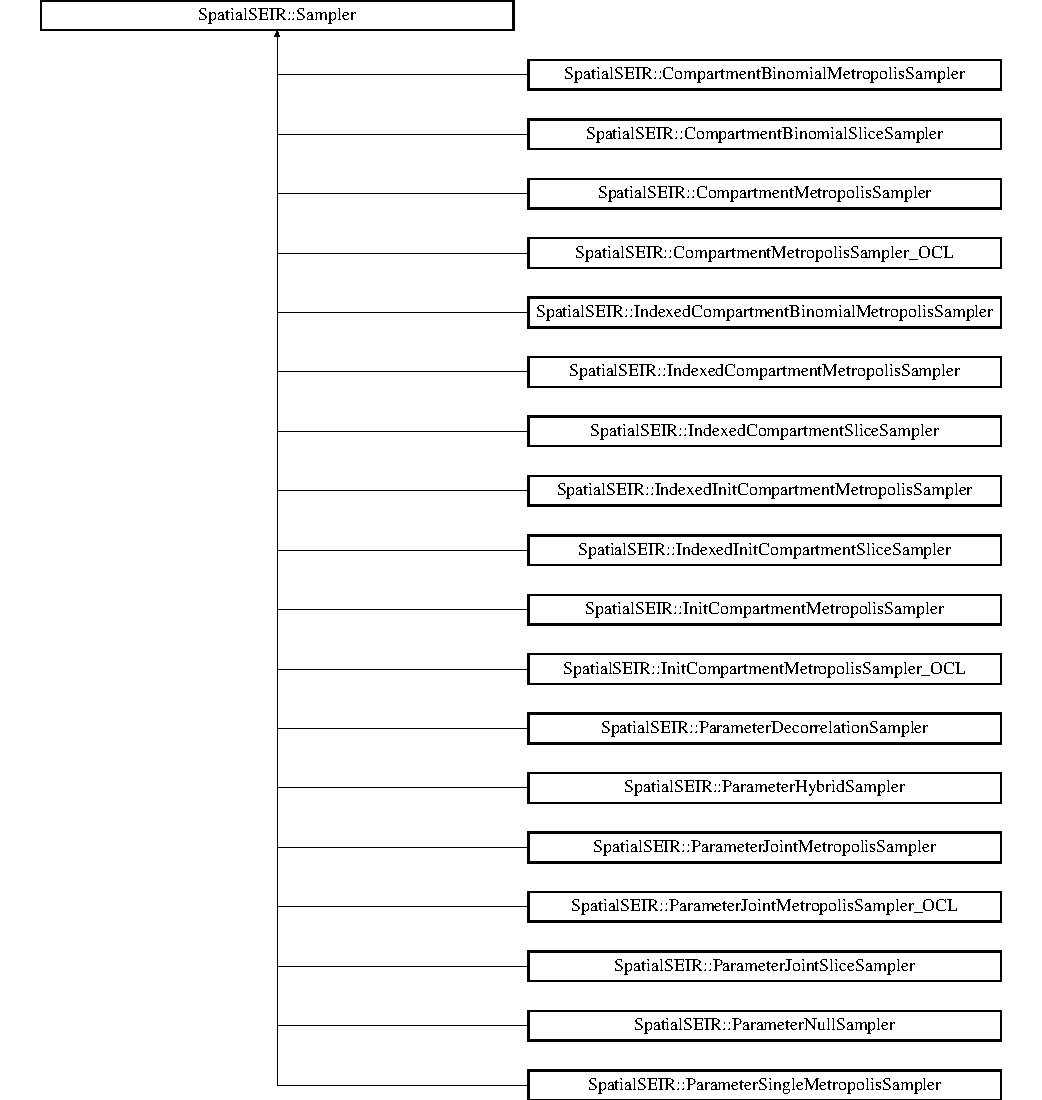
\includegraphics[height=12.000000cm]{classSpatialSEIR_1_1Sampler}
\end{center}
\end{figure}
\subsection*{Public Member Functions}
\begin{DoxyCompactItemize}
\item 
virtual \hyperlink{classSpatialSEIR_1_1Sampler_a2a249720ca17a6ddd53c4f5359cdf739}{$\sim$\-Sampler} ()
\item 
virtual void \hyperlink{classSpatialSEIR_1_1Sampler_aa07a42b26cb62249c20c58e855a08657}{draw\-Sample} ()=0
\item 
virtual int \hyperlink{classSpatialSEIR_1_1Sampler_aaa79310ad809e6aeb25479849f322dda}{get\-Sampler\-Type} ()=0
\end{DoxyCompactItemize}


\subsection{Detailed Description}
The sampler class is the parent class for all M\-C\-M\-C sampler objects, and guarantees that the same high level A\-P\-I applies to all such objects. 

\subsection{Constructor \& Destructor Documentation}
\hypertarget{classSpatialSEIR_1_1Sampler_a2a249720ca17a6ddd53c4f5359cdf739}{\index{Spatial\-S\-E\-I\-R\-::\-Sampler@{Spatial\-S\-E\-I\-R\-::\-Sampler}!$\sim$\-Sampler@{$\sim$\-Sampler}}
\index{$\sim$\-Sampler@{$\sim$\-Sampler}!SpatialSEIR::Sampler@{Spatial\-S\-E\-I\-R\-::\-Sampler}}
\subsubsection[{$\sim$\-Sampler}]{\setlength{\rightskip}{0pt plus 5cm}virtual Spatial\-S\-E\-I\-R\-::\-Sampler\-::$\sim$\-Sampler (
\begin{DoxyParamCaption}
{}
\end{DoxyParamCaption}
)\hspace{0.3cm}{\ttfamily [inline]}, {\ttfamily [virtual]}}}\label{classSpatialSEIR_1_1Sampler_a2a249720ca17a6ddd53c4f5359cdf739}


\subsection{Member Function Documentation}
\hypertarget{classSpatialSEIR_1_1Sampler_aa07a42b26cb62249c20c58e855a08657}{\index{Spatial\-S\-E\-I\-R\-::\-Sampler@{Spatial\-S\-E\-I\-R\-::\-Sampler}!draw\-Sample@{draw\-Sample}}
\index{draw\-Sample@{draw\-Sample}!SpatialSEIR::Sampler@{Spatial\-S\-E\-I\-R\-::\-Sampler}}
\subsubsection[{draw\-Sample}]{\setlength{\rightskip}{0pt plus 5cm}virtual void Spatial\-S\-E\-I\-R\-::\-Sampler\-::draw\-Sample (
\begin{DoxyParamCaption}
{}
\end{DoxyParamCaption}
)\hspace{0.3cm}{\ttfamily [pure virtual]}}}\label{classSpatialSEIR_1_1Sampler_aa07a42b26cb62249c20c58e855a08657}


Implemented in \hyperlink{classSpatialSEIR_1_1ParameterDecorrelationSampler_ad1242cb40cf8a47667b3cbe82eff9c47}{Spatial\-S\-E\-I\-R\-::\-Parameter\-Decorrelation\-Sampler}, \hyperlink{classSpatialSEIR_1_1ParameterJointSliceSampler_aceea42431db7eee7f58d4852cc8d1462}{Spatial\-S\-E\-I\-R\-::\-Parameter\-Joint\-Slice\-Sampler}, \hyperlink{classSpatialSEIR_1_1ParameterJointMetropolisSampler__OCL_a21b7e344e6145b14db9cce5212c74d18}{Spatial\-S\-E\-I\-R\-::\-Parameter\-Joint\-Metropolis\-Sampler\-\_\-\-O\-C\-L}, \hyperlink{classSpatialSEIR_1_1ParameterJointMetropolisSampler_a1224be64e1a5e46290c6f2d95b13fec7}{Spatial\-S\-E\-I\-R\-::\-Parameter\-Joint\-Metropolis\-Sampler}, \hyperlink{classSpatialSEIR_1_1ParameterSingleMetropolisSampler_a637d48dfe689654490ab568e22e6037c}{Spatial\-S\-E\-I\-R\-::\-Parameter\-Single\-Metropolis\-Sampler}, \hyperlink{classSpatialSEIR_1_1IndexedInitCompartmentSliceSampler_a2ff3fc36c3cfc5b49c58234376ba0a1b}{Spatial\-S\-E\-I\-R\-::\-Indexed\-Init\-Compartment\-Slice\-Sampler}, \hyperlink{classSpatialSEIR_1_1IndexedInitCompartmentMetropolisSampler_ad8ee467d7679fa760db613075c9e0db2}{Spatial\-S\-E\-I\-R\-::\-Indexed\-Init\-Compartment\-Metropolis\-Sampler}, \hyperlink{classSpatialSEIR_1_1InitCompartmentMetropolisSampler__OCL_aeb2831c79b43252f3a2a48f405cfccbe}{Spatial\-S\-E\-I\-R\-::\-Init\-Compartment\-Metropolis\-Sampler\-\_\-\-O\-C\-L}, \hyperlink{classSpatialSEIR_1_1InitCompartmentMetropolisSampler_a24aba18be0f06df089897aa471aa8a86}{Spatial\-S\-E\-I\-R\-::\-Init\-Compartment\-Metropolis\-Sampler}, \hyperlink{classSpatialSEIR_1_1CompartmentBinomialSliceSampler_a6d89f57c350e131068718374ae0d135f}{Spatial\-S\-E\-I\-R\-::\-Compartment\-Binomial\-Slice\-Sampler}, \hyperlink{classSpatialSEIR_1_1IndexedCompartmentBinomialMetropolisSampler_a3f172aba5d9389b2193200a811d12142}{Spatial\-S\-E\-I\-R\-::\-Indexed\-Compartment\-Binomial\-Metropolis\-Sampler}, \hyperlink{classSpatialSEIR_1_1CompartmentBinomialMetropolisSampler_a11d2900ff89a59f71e2ff5695432e036}{Spatial\-S\-E\-I\-R\-::\-Compartment\-Binomial\-Metropolis\-Sampler}, \hyperlink{classSpatialSEIR_1_1IndexedCompartmentSliceSampler_aba6f0bd34d4fc684ac844767a09dab95}{Spatial\-S\-E\-I\-R\-::\-Indexed\-Compartment\-Slice\-Sampler}, \hyperlink{classSpatialSEIR_1_1IndexedCompartmentMetropolisSampler_a98bcf6dc5e426a45ef11bf04c1e178dd}{Spatial\-S\-E\-I\-R\-::\-Indexed\-Compartment\-Metropolis\-Sampler}, \hyperlink{classSpatialSEIR_1_1CompartmentMetropolisSampler__OCL_a7a0a9120eab5a44797f9255df6f89c2a}{Spatial\-S\-E\-I\-R\-::\-Compartment\-Metropolis\-Sampler\-\_\-\-O\-C\-L}, \hyperlink{classSpatialSEIR_1_1CompartmentMetropolisSampler_a9d19f29ea0a8b86abb3e2082b469aed5}{Spatial\-S\-E\-I\-R\-::\-Compartment\-Metropolis\-Sampler}, and \hyperlink{classSpatialSEIR_1_1ParameterHybridSampler_a48bdd9605070604d06bcd576919a06f6}{Spatial\-S\-E\-I\-R\-::\-Parameter\-Hybrid\-Sampler}.

\hypertarget{classSpatialSEIR_1_1Sampler_aaa79310ad809e6aeb25479849f322dda}{\index{Spatial\-S\-E\-I\-R\-::\-Sampler@{Spatial\-S\-E\-I\-R\-::\-Sampler}!get\-Sampler\-Type@{get\-Sampler\-Type}}
\index{get\-Sampler\-Type@{get\-Sampler\-Type}!SpatialSEIR::Sampler@{Spatial\-S\-E\-I\-R\-::\-Sampler}}
\subsubsection[{get\-Sampler\-Type}]{\setlength{\rightskip}{0pt plus 5cm}virtual int Spatial\-S\-E\-I\-R\-::\-Sampler\-::get\-Sampler\-Type (
\begin{DoxyParamCaption}
{}
\end{DoxyParamCaption}
)\hspace{0.3cm}{\ttfamily [pure virtual]}}}\label{classSpatialSEIR_1_1Sampler_aaa79310ad809e6aeb25479849f322dda}


Implemented in \hyperlink{classSpatialSEIR_1_1ParameterDecorrelationSampler_ad3039ef7f917ec85fc210be2940b5da1}{Spatial\-S\-E\-I\-R\-::\-Parameter\-Decorrelation\-Sampler}, \hyperlink{classSpatialSEIR_1_1ParameterJointSliceSampler_ac435f72bd91e0585b45d42233b0741dc}{Spatial\-S\-E\-I\-R\-::\-Parameter\-Joint\-Slice\-Sampler}, \hyperlink{classSpatialSEIR_1_1ParameterJointMetropolisSampler__OCL_a1049eea747bcdaa8112defcc52a651d5}{Spatial\-S\-E\-I\-R\-::\-Parameter\-Joint\-Metropolis\-Sampler\-\_\-\-O\-C\-L}, \hyperlink{classSpatialSEIR_1_1ParameterJointMetropolisSampler_a5684e2933ff1fab50e1761450ba41897}{Spatial\-S\-E\-I\-R\-::\-Parameter\-Joint\-Metropolis\-Sampler}, \hyperlink{classSpatialSEIR_1_1ParameterSingleMetropolisSampler_a0576cfdda14e0afb0f63413f01a82c13}{Spatial\-S\-E\-I\-R\-::\-Parameter\-Single\-Metropolis\-Sampler}, \hyperlink{classSpatialSEIR_1_1IndexedInitCompartmentSliceSampler_a8687c4d1acc384cc4e8d7f4b91db79a5}{Spatial\-S\-E\-I\-R\-::\-Indexed\-Init\-Compartment\-Slice\-Sampler}, \hyperlink{classSpatialSEIR_1_1IndexedInitCompartmentMetropolisSampler_af2891523864f89b9587205eaba4bd41a}{Spatial\-S\-E\-I\-R\-::\-Indexed\-Init\-Compartment\-Metropolis\-Sampler}, \hyperlink{classSpatialSEIR_1_1InitCompartmentMetropolisSampler__OCL_a932637bc74c6f2f5fc251dd4a81131ae}{Spatial\-S\-E\-I\-R\-::\-Init\-Compartment\-Metropolis\-Sampler\-\_\-\-O\-C\-L}, \hyperlink{classSpatialSEIR_1_1InitCompartmentMetropolisSampler_ad64b5ae0943c980f752c49f9c179a3b7}{Spatial\-S\-E\-I\-R\-::\-Init\-Compartment\-Metropolis\-Sampler}, \hyperlink{classSpatialSEIR_1_1CompartmentBinomialSliceSampler_a35f2ba8531217f1fa227da3b801d05dd}{Spatial\-S\-E\-I\-R\-::\-Compartment\-Binomial\-Slice\-Sampler}, \hyperlink{classSpatialSEIR_1_1IndexedCompartmentBinomialMetropolisSampler_a2ce0af7bb2a881f254dfbd97584704bd}{Spatial\-S\-E\-I\-R\-::\-Indexed\-Compartment\-Binomial\-Metropolis\-Sampler}, \hyperlink{classSpatialSEIR_1_1CompartmentBinomialMetropolisSampler_aa84f51d4d02943be01c6309581ecc17a}{Spatial\-S\-E\-I\-R\-::\-Compartment\-Binomial\-Metropolis\-Sampler}, \hyperlink{classSpatialSEIR_1_1IndexedCompartmentSliceSampler_aeeeeb33f86bf684e6e44914c784847e6}{Spatial\-S\-E\-I\-R\-::\-Indexed\-Compartment\-Slice\-Sampler}, \hyperlink{classSpatialSEIR_1_1IndexedCompartmentMetropolisSampler_a87fe511f9a9fd517c4bafad59c296986}{Spatial\-S\-E\-I\-R\-::\-Indexed\-Compartment\-Metropolis\-Sampler}, \hyperlink{classSpatialSEIR_1_1CompartmentMetropolisSampler__OCL_a15b18cebae437f578fbf15aa8cfbdf94}{Spatial\-S\-E\-I\-R\-::\-Compartment\-Metropolis\-Sampler\-\_\-\-O\-C\-L}, \hyperlink{classSpatialSEIR_1_1CompartmentMetropolisSampler_a249b461e6f848c20f274bac7cae76e95}{Spatial\-S\-E\-I\-R\-::\-Compartment\-Metropolis\-Sampler}, and \hyperlink{classSpatialSEIR_1_1ParameterHybridSampler_ae5c2d418521cc111a5f6e92e995f823c}{Spatial\-S\-E\-I\-R\-::\-Parameter\-Hybrid\-Sampler}.



The documentation for this class was generated from the following file\-:\begin{DoxyCompactItemize}
\item 
lib\-Spatial\-S\-E\-I\-R/include/\hyperlink{LSS__Samplers_8hpp}{L\-S\-S\-\_\-\-Samplers.\-hpp}\end{DoxyCompactItemize}

\hypertarget{structSpatialSEIR_1_1scaledDistanceArgs}{\section{Spatial\-S\-E\-I\-R\-:\-:scaled\-Distance\-Args Struct Reference}
\label{structSpatialSEIR_1_1scaledDistanceArgs}\index{Spatial\-S\-E\-I\-R\-::scaled\-Distance\-Args@{Spatial\-S\-E\-I\-R\-::scaled\-Distance\-Args}}
}


{\ttfamily \#include $<$Distance\-Matrix.\-hpp$>$}

\subsection*{Public Attributes}
\begin{DoxyCompactItemize}
\item 
double $\ast$ \hyperlink{structSpatialSEIR_1_1scaledDistanceArgs_ade9b8cabc3faa5a2a8c27c18d1a99ec6}{phi}
\item 
std\-::vector$<$ double $\ast$ $>$ \hyperlink{structSpatialSEIR_1_1scaledDistanceArgs_a2f088ea1220ce3eb17762e7ee51c5249}{in\-Data}
\item 
int $\ast$ \hyperlink{structSpatialSEIR_1_1scaledDistanceArgs_a298c111f01f4b8d7950c6b83532fbd97}{dim}
\item 
int \hyperlink{structSpatialSEIR_1_1scaledDistanceArgs_ad9c4a2a8701453b54110ad51164aa39e}{mode}
\end{DoxyCompactItemize}


\subsection{Member Data Documentation}
\hypertarget{structSpatialSEIR_1_1scaledDistanceArgs_a298c111f01f4b8d7950c6b83532fbd97}{\index{Spatial\-S\-E\-I\-R\-::scaled\-Distance\-Args@{Spatial\-S\-E\-I\-R\-::scaled\-Distance\-Args}!dim@{dim}}
\index{dim@{dim}!SpatialSEIR::scaledDistanceArgs@{Spatial\-S\-E\-I\-R\-::scaled\-Distance\-Args}}
\subsubsection[{dim}]{\setlength{\rightskip}{0pt plus 5cm}int$\ast$ Spatial\-S\-E\-I\-R\-::scaled\-Distance\-Args\-::dim}}\label{structSpatialSEIR_1_1scaledDistanceArgs_a298c111f01f4b8d7950c6b83532fbd97}
\hypertarget{structSpatialSEIR_1_1scaledDistanceArgs_a2f088ea1220ce3eb17762e7ee51c5249}{\index{Spatial\-S\-E\-I\-R\-::scaled\-Distance\-Args@{Spatial\-S\-E\-I\-R\-::scaled\-Distance\-Args}!in\-Data@{in\-Data}}
\index{in\-Data@{in\-Data}!SpatialSEIR::scaledDistanceArgs@{Spatial\-S\-E\-I\-R\-::scaled\-Distance\-Args}}
\subsubsection[{in\-Data}]{\setlength{\rightskip}{0pt plus 5cm}std\-::vector$<$double$\ast$$>$ Spatial\-S\-E\-I\-R\-::scaled\-Distance\-Args\-::in\-Data}}\label{structSpatialSEIR_1_1scaledDistanceArgs_a2f088ea1220ce3eb17762e7ee51c5249}
\hypertarget{structSpatialSEIR_1_1scaledDistanceArgs_ad9c4a2a8701453b54110ad51164aa39e}{\index{Spatial\-S\-E\-I\-R\-::scaled\-Distance\-Args@{Spatial\-S\-E\-I\-R\-::scaled\-Distance\-Args}!mode@{mode}}
\index{mode@{mode}!SpatialSEIR::scaledDistanceArgs@{Spatial\-S\-E\-I\-R\-::scaled\-Distance\-Args}}
\subsubsection[{mode}]{\setlength{\rightskip}{0pt plus 5cm}int Spatial\-S\-E\-I\-R\-::scaled\-Distance\-Args\-::mode}}\label{structSpatialSEIR_1_1scaledDistanceArgs_ad9c4a2a8701453b54110ad51164aa39e}
\hypertarget{structSpatialSEIR_1_1scaledDistanceArgs_ade9b8cabc3faa5a2a8c27c18d1a99ec6}{\index{Spatial\-S\-E\-I\-R\-::scaled\-Distance\-Args@{Spatial\-S\-E\-I\-R\-::scaled\-Distance\-Args}!phi@{phi}}
\index{phi@{phi}!SpatialSEIR::scaledDistanceArgs@{Spatial\-S\-E\-I\-R\-::scaled\-Distance\-Args}}
\subsubsection[{phi}]{\setlength{\rightskip}{0pt plus 5cm}double$\ast$ Spatial\-S\-E\-I\-R\-::scaled\-Distance\-Args\-::phi}}\label{structSpatialSEIR_1_1scaledDistanceArgs_ade9b8cabc3faa5a2a8c27c18d1a99ec6}


The documentation for this struct was generated from the following file\-:\begin{DoxyCompactItemize}
\item 
lib\-Spatial\-S\-E\-I\-R/include/\-Data\-Structures/\hyperlink{DistanceMatrix_8hpp}{Distance\-Matrix.\-hpp}\end{DoxyCompactItemize}

\hypertarget{classSpatialSEIR_1_1SetCompartmentSamplingIndicesTask}{\section{Spatial\-S\-E\-I\-R\-:\-:Set\-Compartment\-Sampling\-Indices\-Task Class Reference}
\label{classSpatialSEIR_1_1SetCompartmentSamplingIndicesTask}\index{Spatial\-S\-E\-I\-R\-::\-Set\-Compartment\-Sampling\-Indices\-Task@{Spatial\-S\-E\-I\-R\-::\-Set\-Compartment\-Sampling\-Indices\-Task}}
}


{\ttfamily \#include $<$L\-S\-S\-\_\-\-Iteration\-Tasks.\-hpp$>$}

Inheritance diagram for Spatial\-S\-E\-I\-R\-:\-:Set\-Compartment\-Sampling\-Indices\-Task\-:\begin{figure}[H]
\begin{center}
\leavevmode
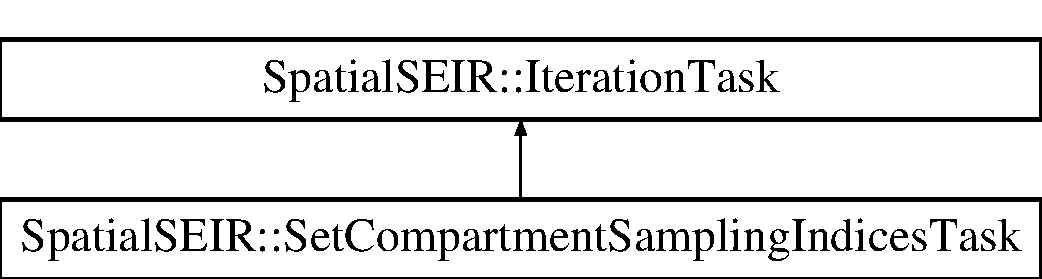
\includegraphics[height=2.000000cm]{classSpatialSEIR_1_1SetCompartmentSamplingIndicesTask}
\end{center}
\end{figure}
\subsection*{Public Member Functions}
\begin{DoxyCompactItemize}
\item 
\hyperlink{classSpatialSEIR_1_1SetCompartmentSamplingIndicesTask_a2f292054f24192f3b6e9ce7b63fa297b}{Set\-Compartment\-Sampling\-Indices\-Task} (\hyperlink{classSpatialSEIR_1_1ModelContext}{Model\-Context} $\ast$\hyperlink{classSpatialSEIR_1_1SetCompartmentSamplingIndicesTask_a52dd5ee41a16c253719145db4619f21d}{context})
\item 
\hyperlink{classSpatialSEIR_1_1SetCompartmentSamplingIndicesTask_a5d9804f091418dfead47b7bd284ffd29}{$\sim$\-Set\-Compartment\-Sampling\-Indices\-Task} ()
\item 
void \hyperlink{classSpatialSEIR_1_1SetCompartmentSamplingIndicesTask_aebbc3bb4337fe6ce5c2f81335489c4df}{execute\-Task} ()
\item 
int \hyperlink{classSpatialSEIR_1_1SetCompartmentSamplingIndicesTask_ae48bddebfa315cf138729bc90f24abc0}{get\-Task\-Type} ()
\end{DoxyCompactItemize}
\subsection*{Public Attributes}
\begin{DoxyCompactItemize}
\item 
\hyperlink{classSpatialSEIR_1_1ModelContext}{Model\-Context} $\ast$$\ast$ \hyperlink{classSpatialSEIR_1_1SetCompartmentSamplingIndicesTask_a52dd5ee41a16c253719145db4619f21d}{context}
\item 
int $\ast$$\ast$ \hyperlink{classSpatialSEIR_1_1SetCompartmentSamplingIndicesTask_aa886632dfda17a6f9a00cb1161685c35}{index}
\item 
int $\ast$$\ast$ \hyperlink{classSpatialSEIR_1_1SetCompartmentSamplingIndicesTask_ae9c42a17508247572b82dd6357ecafed}{index\-Length}
\end{DoxyCompactItemize}


\subsection{Detailed Description}
Several of the compartment sampling classes rely on a list of indices managed by model context to jointly update the same space-\/time locations for each of the compartments in order to reduce sampler autocorrelation. This task updates the list of indices after each M\-C\-M\-C sample. 

\subsection{Constructor \& Destructor Documentation}
\hypertarget{classSpatialSEIR_1_1SetCompartmentSamplingIndicesTask_a2f292054f24192f3b6e9ce7b63fa297b}{\index{Spatial\-S\-E\-I\-R\-::\-Set\-Compartment\-Sampling\-Indices\-Task@{Spatial\-S\-E\-I\-R\-::\-Set\-Compartment\-Sampling\-Indices\-Task}!Set\-Compartment\-Sampling\-Indices\-Task@{Set\-Compartment\-Sampling\-Indices\-Task}}
\index{Set\-Compartment\-Sampling\-Indices\-Task@{Set\-Compartment\-Sampling\-Indices\-Task}!SpatialSEIR::SetCompartmentSamplingIndicesTask@{Spatial\-S\-E\-I\-R\-::\-Set\-Compartment\-Sampling\-Indices\-Task}}
\subsubsection[{Set\-Compartment\-Sampling\-Indices\-Task}]{\setlength{\rightskip}{0pt plus 5cm}Spatial\-S\-E\-I\-R\-::\-Set\-Compartment\-Sampling\-Indices\-Task\-::\-Set\-Compartment\-Sampling\-Indices\-Task (
\begin{DoxyParamCaption}
\item[{{\bf Model\-Context} $\ast$}]{context}
\end{DoxyParamCaption}
)}}\label{classSpatialSEIR_1_1SetCompartmentSamplingIndicesTask_a2f292054f24192f3b6e9ce7b63fa297b}
\hypertarget{classSpatialSEIR_1_1SetCompartmentSamplingIndicesTask_a5d9804f091418dfead47b7bd284ffd29}{\index{Spatial\-S\-E\-I\-R\-::\-Set\-Compartment\-Sampling\-Indices\-Task@{Spatial\-S\-E\-I\-R\-::\-Set\-Compartment\-Sampling\-Indices\-Task}!$\sim$\-Set\-Compartment\-Sampling\-Indices\-Task@{$\sim$\-Set\-Compartment\-Sampling\-Indices\-Task}}
\index{$\sim$\-Set\-Compartment\-Sampling\-Indices\-Task@{$\sim$\-Set\-Compartment\-Sampling\-Indices\-Task}!SpatialSEIR::SetCompartmentSamplingIndicesTask@{Spatial\-S\-E\-I\-R\-::\-Set\-Compartment\-Sampling\-Indices\-Task}}
\subsubsection[{$\sim$\-Set\-Compartment\-Sampling\-Indices\-Task}]{\setlength{\rightskip}{0pt plus 5cm}Spatial\-S\-E\-I\-R\-::\-Set\-Compartment\-Sampling\-Indices\-Task\-::$\sim$\-Set\-Compartment\-Sampling\-Indices\-Task (
\begin{DoxyParamCaption}
{}
\end{DoxyParamCaption}
)}}\label{classSpatialSEIR_1_1SetCompartmentSamplingIndicesTask_a5d9804f091418dfead47b7bd284ffd29}


\subsection{Member Function Documentation}
\hypertarget{classSpatialSEIR_1_1SetCompartmentSamplingIndicesTask_aebbc3bb4337fe6ce5c2f81335489c4df}{\index{Spatial\-S\-E\-I\-R\-::\-Set\-Compartment\-Sampling\-Indices\-Task@{Spatial\-S\-E\-I\-R\-::\-Set\-Compartment\-Sampling\-Indices\-Task}!execute\-Task@{execute\-Task}}
\index{execute\-Task@{execute\-Task}!SpatialSEIR::SetCompartmentSamplingIndicesTask@{Spatial\-S\-E\-I\-R\-::\-Set\-Compartment\-Sampling\-Indices\-Task}}
\subsubsection[{execute\-Task}]{\setlength{\rightskip}{0pt plus 5cm}void Spatial\-S\-E\-I\-R\-::\-Set\-Compartment\-Sampling\-Indices\-Task\-::execute\-Task (
\begin{DoxyParamCaption}
{}
\end{DoxyParamCaption}
)\hspace{0.3cm}{\ttfamily [virtual]}}}\label{classSpatialSEIR_1_1SetCompartmentSamplingIndicesTask_aebbc3bb4337fe6ce5c2f81335489c4df}


Implements \hyperlink{classSpatialSEIR_1_1IterationTask_a68fcb08fe777ed506c97dc1ac5a0fb54}{Spatial\-S\-E\-I\-R\-::\-Iteration\-Task}.

\hypertarget{classSpatialSEIR_1_1SetCompartmentSamplingIndicesTask_ae48bddebfa315cf138729bc90f24abc0}{\index{Spatial\-S\-E\-I\-R\-::\-Set\-Compartment\-Sampling\-Indices\-Task@{Spatial\-S\-E\-I\-R\-::\-Set\-Compartment\-Sampling\-Indices\-Task}!get\-Task\-Type@{get\-Task\-Type}}
\index{get\-Task\-Type@{get\-Task\-Type}!SpatialSEIR::SetCompartmentSamplingIndicesTask@{Spatial\-S\-E\-I\-R\-::\-Set\-Compartment\-Sampling\-Indices\-Task}}
\subsubsection[{get\-Task\-Type}]{\setlength{\rightskip}{0pt plus 5cm}int Spatial\-S\-E\-I\-R\-::\-Set\-Compartment\-Sampling\-Indices\-Task\-::get\-Task\-Type (
\begin{DoxyParamCaption}
{}
\end{DoxyParamCaption}
)\hspace{0.3cm}{\ttfamily [virtual]}}}\label{classSpatialSEIR_1_1SetCompartmentSamplingIndicesTask_ae48bddebfa315cf138729bc90f24abc0}


Implements \hyperlink{classSpatialSEIR_1_1IterationTask_aaba9c737c4564df6b44b843d7c781722}{Spatial\-S\-E\-I\-R\-::\-Iteration\-Task}.



\subsection{Member Data Documentation}
\hypertarget{classSpatialSEIR_1_1SetCompartmentSamplingIndicesTask_a52dd5ee41a16c253719145db4619f21d}{\index{Spatial\-S\-E\-I\-R\-::\-Set\-Compartment\-Sampling\-Indices\-Task@{Spatial\-S\-E\-I\-R\-::\-Set\-Compartment\-Sampling\-Indices\-Task}!context@{context}}
\index{context@{context}!SpatialSEIR::SetCompartmentSamplingIndicesTask@{Spatial\-S\-E\-I\-R\-::\-Set\-Compartment\-Sampling\-Indices\-Task}}
\subsubsection[{context}]{\setlength{\rightskip}{0pt plus 5cm}{\bf Model\-Context}$\ast$$\ast$ Spatial\-S\-E\-I\-R\-::\-Set\-Compartment\-Sampling\-Indices\-Task\-::context}}\label{classSpatialSEIR_1_1SetCompartmentSamplingIndicesTask_a52dd5ee41a16c253719145db4619f21d}
\hypertarget{classSpatialSEIR_1_1SetCompartmentSamplingIndicesTask_aa886632dfda17a6f9a00cb1161685c35}{\index{Spatial\-S\-E\-I\-R\-::\-Set\-Compartment\-Sampling\-Indices\-Task@{Spatial\-S\-E\-I\-R\-::\-Set\-Compartment\-Sampling\-Indices\-Task}!index@{index}}
\index{index@{index}!SpatialSEIR::SetCompartmentSamplingIndicesTask@{Spatial\-S\-E\-I\-R\-::\-Set\-Compartment\-Sampling\-Indices\-Task}}
\subsubsection[{index}]{\setlength{\rightskip}{0pt plus 5cm}int$\ast$$\ast$ Spatial\-S\-E\-I\-R\-::\-Set\-Compartment\-Sampling\-Indices\-Task\-::index}}\label{classSpatialSEIR_1_1SetCompartmentSamplingIndicesTask_aa886632dfda17a6f9a00cb1161685c35}
\hypertarget{classSpatialSEIR_1_1SetCompartmentSamplingIndicesTask_ae9c42a17508247572b82dd6357ecafed}{\index{Spatial\-S\-E\-I\-R\-::\-Set\-Compartment\-Sampling\-Indices\-Task@{Spatial\-S\-E\-I\-R\-::\-Set\-Compartment\-Sampling\-Indices\-Task}!index\-Length@{index\-Length}}
\index{index\-Length@{index\-Length}!SpatialSEIR::SetCompartmentSamplingIndicesTask@{Spatial\-S\-E\-I\-R\-::\-Set\-Compartment\-Sampling\-Indices\-Task}}
\subsubsection[{index\-Length}]{\setlength{\rightskip}{0pt plus 5cm}int$\ast$$\ast$ Spatial\-S\-E\-I\-R\-::\-Set\-Compartment\-Sampling\-Indices\-Task\-::index\-Length}}\label{classSpatialSEIR_1_1SetCompartmentSamplingIndicesTask_ae9c42a17508247572b82dd6357ecafed}


The documentation for this class was generated from the following file\-:\begin{DoxyCompactItemize}
\item 
lib\-Spatial\-S\-E\-I\-R/include/\hyperlink{LSS__IterationTasks_8hpp}{L\-S\-S\-\_\-\-Iteration\-Tasks.\-hpp}\end{DoxyCompactItemize}

\hypertarget{structSpatialSEIR_1_1sliceParameters}{\section{Spatial\-S\-E\-I\-R\-:\-:slice\-Parameters Struct Reference}
\label{structSpatialSEIR_1_1sliceParameters}\index{Spatial\-S\-E\-I\-R\-::slice\-Parameters@{Spatial\-S\-E\-I\-R\-::slice\-Parameters}}
}


struct containing initial slice sampling tuning parameters.  




{\ttfamily \#include $<$L\-S\-S\-\_\-\-Full\-Conditional.\-hpp$>$}

\subsection*{Public Attributes}
\begin{DoxyCompactItemize}
\item 
double $\ast$ \hyperlink{structSpatialSEIR_1_1sliceParameters_a2f90b463a0c19e9ddee18b6b7201aa3a}{S\-\_\-star\-Width}
\item 
double $\ast$ \hyperlink{structSpatialSEIR_1_1sliceParameters_af81f880dad34e409ec23d3dee95cde9d}{E\-\_\-star\-Width}
\item 
double $\ast$ \hyperlink{structSpatialSEIR_1_1sliceParameters_a11f8948e29f2b1753c34b3665de8b0a5}{R\-\_\-star\-Width}
\item 
double $\ast$ \hyperlink{structSpatialSEIR_1_1sliceParameters_a2413af0d867a2b39d3d614bfc61b1a08}{S0\-Width}
\item 
double $\ast$ \hyperlink{structSpatialSEIR_1_1sliceParameters_af927171f24f8b4f4f4f44cbc3dcabb2a}{I0\-Width}
\item 
double $\ast$ \hyperlink{structSpatialSEIR_1_1sliceParameters_a890369737115cf27a7f5f86fca564248}{beta\-Width}
\item 
double $\ast$ \hyperlink{structSpatialSEIR_1_1sliceParameters_a1e503332bf376006b6e46c4f5eb2c1ab}{beta\-Prs\-Width}
\item 
double $\ast$ \hyperlink{structSpatialSEIR_1_1sliceParameters_a484236433bd95049ce83b7fbfe90407f}{rho\-Width}
\item 
double $\ast$ \hyperlink{structSpatialSEIR_1_1sliceParameters_aa390f8753fbf788e73dcd9c865fd78ee}{gamma\-Ei\-Width}
\item 
double $\ast$ \hyperlink{structSpatialSEIR_1_1sliceParameters_aa6e7b44947455b6376ef7eb2258e599f}{gamma\-Ir\-Width}
\item 
double $\ast$ \hyperlink{structSpatialSEIR_1_1sliceParameters_a11c8c9bdef914a68fce64b75ee19752c}{phi\-Width}
\end{DoxyCompactItemize}


\subsection{Detailed Description}
struct containing initial slice sampling tuning parameters. 

\subsection{Member Data Documentation}
\hypertarget{structSpatialSEIR_1_1sliceParameters_a1e503332bf376006b6e46c4f5eb2c1ab}{\index{Spatial\-S\-E\-I\-R\-::slice\-Parameters@{Spatial\-S\-E\-I\-R\-::slice\-Parameters}!beta\-Prs\-Width@{beta\-Prs\-Width}}
\index{beta\-Prs\-Width@{beta\-Prs\-Width}!SpatialSEIR::sliceParameters@{Spatial\-S\-E\-I\-R\-::slice\-Parameters}}
\subsubsection[{beta\-Prs\-Width}]{\setlength{\rightskip}{0pt plus 5cm}double$\ast$ Spatial\-S\-E\-I\-R\-::slice\-Parameters\-::beta\-Prs\-Width}}\label{structSpatialSEIR_1_1sliceParameters_a1e503332bf376006b6e46c4f5eb2c1ab}
\hypertarget{structSpatialSEIR_1_1sliceParameters_a890369737115cf27a7f5f86fca564248}{\index{Spatial\-S\-E\-I\-R\-::slice\-Parameters@{Spatial\-S\-E\-I\-R\-::slice\-Parameters}!beta\-Width@{beta\-Width}}
\index{beta\-Width@{beta\-Width}!SpatialSEIR::sliceParameters@{Spatial\-S\-E\-I\-R\-::slice\-Parameters}}
\subsubsection[{beta\-Width}]{\setlength{\rightskip}{0pt plus 5cm}double$\ast$ Spatial\-S\-E\-I\-R\-::slice\-Parameters\-::beta\-Width}}\label{structSpatialSEIR_1_1sliceParameters_a890369737115cf27a7f5f86fca564248}
\hypertarget{structSpatialSEIR_1_1sliceParameters_af81f880dad34e409ec23d3dee95cde9d}{\index{Spatial\-S\-E\-I\-R\-::slice\-Parameters@{Spatial\-S\-E\-I\-R\-::slice\-Parameters}!E\-\_\-star\-Width@{E\-\_\-star\-Width}}
\index{E\-\_\-star\-Width@{E\-\_\-star\-Width}!SpatialSEIR::sliceParameters@{Spatial\-S\-E\-I\-R\-::slice\-Parameters}}
\subsubsection[{E\-\_\-star\-Width}]{\setlength{\rightskip}{0pt plus 5cm}double$\ast$ Spatial\-S\-E\-I\-R\-::slice\-Parameters\-::\-E\-\_\-star\-Width}}\label{structSpatialSEIR_1_1sliceParameters_af81f880dad34e409ec23d3dee95cde9d}
\hypertarget{structSpatialSEIR_1_1sliceParameters_aa390f8753fbf788e73dcd9c865fd78ee}{\index{Spatial\-S\-E\-I\-R\-::slice\-Parameters@{Spatial\-S\-E\-I\-R\-::slice\-Parameters}!gamma\-Ei\-Width@{gamma\-Ei\-Width}}
\index{gamma\-Ei\-Width@{gamma\-Ei\-Width}!SpatialSEIR::sliceParameters@{Spatial\-S\-E\-I\-R\-::slice\-Parameters}}
\subsubsection[{gamma\-Ei\-Width}]{\setlength{\rightskip}{0pt plus 5cm}double$\ast$ Spatial\-S\-E\-I\-R\-::slice\-Parameters\-::gamma\-Ei\-Width}}\label{structSpatialSEIR_1_1sliceParameters_aa390f8753fbf788e73dcd9c865fd78ee}
\hypertarget{structSpatialSEIR_1_1sliceParameters_aa6e7b44947455b6376ef7eb2258e599f}{\index{Spatial\-S\-E\-I\-R\-::slice\-Parameters@{Spatial\-S\-E\-I\-R\-::slice\-Parameters}!gamma\-Ir\-Width@{gamma\-Ir\-Width}}
\index{gamma\-Ir\-Width@{gamma\-Ir\-Width}!SpatialSEIR::sliceParameters@{Spatial\-S\-E\-I\-R\-::slice\-Parameters}}
\subsubsection[{gamma\-Ir\-Width}]{\setlength{\rightskip}{0pt plus 5cm}double$\ast$ Spatial\-S\-E\-I\-R\-::slice\-Parameters\-::gamma\-Ir\-Width}}\label{structSpatialSEIR_1_1sliceParameters_aa6e7b44947455b6376ef7eb2258e599f}
\hypertarget{structSpatialSEIR_1_1sliceParameters_af927171f24f8b4f4f4f44cbc3dcabb2a}{\index{Spatial\-S\-E\-I\-R\-::slice\-Parameters@{Spatial\-S\-E\-I\-R\-::slice\-Parameters}!I0\-Width@{I0\-Width}}
\index{I0\-Width@{I0\-Width}!SpatialSEIR::sliceParameters@{Spatial\-S\-E\-I\-R\-::slice\-Parameters}}
\subsubsection[{I0\-Width}]{\setlength{\rightskip}{0pt plus 5cm}double$\ast$ Spatial\-S\-E\-I\-R\-::slice\-Parameters\-::\-I0\-Width}}\label{structSpatialSEIR_1_1sliceParameters_af927171f24f8b4f4f4f44cbc3dcabb2a}
\hypertarget{structSpatialSEIR_1_1sliceParameters_a11c8c9bdef914a68fce64b75ee19752c}{\index{Spatial\-S\-E\-I\-R\-::slice\-Parameters@{Spatial\-S\-E\-I\-R\-::slice\-Parameters}!phi\-Width@{phi\-Width}}
\index{phi\-Width@{phi\-Width}!SpatialSEIR::sliceParameters@{Spatial\-S\-E\-I\-R\-::slice\-Parameters}}
\subsubsection[{phi\-Width}]{\setlength{\rightskip}{0pt plus 5cm}double$\ast$ Spatial\-S\-E\-I\-R\-::slice\-Parameters\-::phi\-Width}}\label{structSpatialSEIR_1_1sliceParameters_a11c8c9bdef914a68fce64b75ee19752c}
\hypertarget{structSpatialSEIR_1_1sliceParameters_a11f8948e29f2b1753c34b3665de8b0a5}{\index{Spatial\-S\-E\-I\-R\-::slice\-Parameters@{Spatial\-S\-E\-I\-R\-::slice\-Parameters}!R\-\_\-star\-Width@{R\-\_\-star\-Width}}
\index{R\-\_\-star\-Width@{R\-\_\-star\-Width}!SpatialSEIR::sliceParameters@{Spatial\-S\-E\-I\-R\-::slice\-Parameters}}
\subsubsection[{R\-\_\-star\-Width}]{\setlength{\rightskip}{0pt plus 5cm}double$\ast$ Spatial\-S\-E\-I\-R\-::slice\-Parameters\-::\-R\-\_\-star\-Width}}\label{structSpatialSEIR_1_1sliceParameters_a11f8948e29f2b1753c34b3665de8b0a5}
\hypertarget{structSpatialSEIR_1_1sliceParameters_a484236433bd95049ce83b7fbfe90407f}{\index{Spatial\-S\-E\-I\-R\-::slice\-Parameters@{Spatial\-S\-E\-I\-R\-::slice\-Parameters}!rho\-Width@{rho\-Width}}
\index{rho\-Width@{rho\-Width}!SpatialSEIR::sliceParameters@{Spatial\-S\-E\-I\-R\-::slice\-Parameters}}
\subsubsection[{rho\-Width}]{\setlength{\rightskip}{0pt plus 5cm}double$\ast$ Spatial\-S\-E\-I\-R\-::slice\-Parameters\-::rho\-Width}}\label{structSpatialSEIR_1_1sliceParameters_a484236433bd95049ce83b7fbfe90407f}
\hypertarget{structSpatialSEIR_1_1sliceParameters_a2413af0d867a2b39d3d614bfc61b1a08}{\index{Spatial\-S\-E\-I\-R\-::slice\-Parameters@{Spatial\-S\-E\-I\-R\-::slice\-Parameters}!S0\-Width@{S0\-Width}}
\index{S0\-Width@{S0\-Width}!SpatialSEIR::sliceParameters@{Spatial\-S\-E\-I\-R\-::slice\-Parameters}}
\subsubsection[{S0\-Width}]{\setlength{\rightskip}{0pt plus 5cm}double$\ast$ Spatial\-S\-E\-I\-R\-::slice\-Parameters\-::\-S0\-Width}}\label{structSpatialSEIR_1_1sliceParameters_a2413af0d867a2b39d3d614bfc61b1a08}
\hypertarget{structSpatialSEIR_1_1sliceParameters_a2f90b463a0c19e9ddee18b6b7201aa3a}{\index{Spatial\-S\-E\-I\-R\-::slice\-Parameters@{Spatial\-S\-E\-I\-R\-::slice\-Parameters}!S\-\_\-star\-Width@{S\-\_\-star\-Width}}
\index{S\-\_\-star\-Width@{S\-\_\-star\-Width}!SpatialSEIR::sliceParameters@{Spatial\-S\-E\-I\-R\-::slice\-Parameters}}
\subsubsection[{S\-\_\-star\-Width}]{\setlength{\rightskip}{0pt plus 5cm}double$\ast$ Spatial\-S\-E\-I\-R\-::slice\-Parameters\-::\-S\-\_\-star\-Width}}\label{structSpatialSEIR_1_1sliceParameters_a2f90b463a0c19e9ddee18b6b7201aa3a}


The documentation for this struct was generated from the following file\-:\begin{DoxyCompactItemize}
\item 
lib\-Spatial\-S\-E\-I\-R/include/\-Full\-Conditionals/\hyperlink{LSS__FullConditional_8hpp}{L\-S\-S\-\_\-\-Full\-Conditional.\-hpp}\end{DoxyCompactItemize}

\hypertarget{structSpatialSEIR_1_1TimeLocationTrace}{\section{Spatial\-S\-E\-I\-R\-:\-:Time\-Location\-Trace Struct Reference}
\label{structSpatialSEIR_1_1TimeLocationTrace}\index{Spatial\-S\-E\-I\-R\-::\-Time\-Location\-Trace@{Spatial\-S\-E\-I\-R\-::\-Time\-Location\-Trace}}
}


{\ttfamily \#include $<$I\-O\-Provider.\-hpp$>$}

\subsection*{Public Attributes}
\begin{DoxyCompactItemize}
\item 
int \hyperlink{structSpatialSEIR_1_1TimeLocationTrace_a5196dce9802a7e407273f02e4a92aab2}{location\-Index}
\item 
int \hyperlink{structSpatialSEIR_1_1TimeLocationTrace_a5d006c0c9b1226c25baffc56a4736441}{time\-Index}
\end{DoxyCompactItemize}


\subsection{Member Data Documentation}
\hypertarget{structSpatialSEIR_1_1TimeLocationTrace_a5196dce9802a7e407273f02e4a92aab2}{\index{Spatial\-S\-E\-I\-R\-::\-Time\-Location\-Trace@{Spatial\-S\-E\-I\-R\-::\-Time\-Location\-Trace}!location\-Index@{location\-Index}}
\index{location\-Index@{location\-Index}!SpatialSEIR::TimeLocationTrace@{Spatial\-S\-E\-I\-R\-::\-Time\-Location\-Trace}}
\subsubsection[{location\-Index}]{\setlength{\rightskip}{0pt plus 5cm}int Spatial\-S\-E\-I\-R\-::\-Time\-Location\-Trace\-::location\-Index}}\label{structSpatialSEIR_1_1TimeLocationTrace_a5196dce9802a7e407273f02e4a92aab2}
\hypertarget{structSpatialSEIR_1_1TimeLocationTrace_a5d006c0c9b1226c25baffc56a4736441}{\index{Spatial\-S\-E\-I\-R\-::\-Time\-Location\-Trace@{Spatial\-S\-E\-I\-R\-::\-Time\-Location\-Trace}!time\-Index@{time\-Index}}
\index{time\-Index@{time\-Index}!SpatialSEIR::TimeLocationTrace@{Spatial\-S\-E\-I\-R\-::\-Time\-Location\-Trace}}
\subsubsection[{time\-Index}]{\setlength{\rightskip}{0pt plus 5cm}int Spatial\-S\-E\-I\-R\-::\-Time\-Location\-Trace\-::time\-Index}}\label{structSpatialSEIR_1_1TimeLocationTrace_a5d006c0c9b1226c25baffc56a4736441}


The documentation for this struct was generated from the following file\-:\begin{DoxyCompactItemize}
\item 
lib\-Spatial\-S\-E\-I\-R/include/\hyperlink{IOProvider_8hpp}{I\-O\-Provider.\-hpp}\end{DoxyCompactItemize}

\chapter{File Documentation}
\hypertarget{cblas_8h}{\section{lib\-Spatial\-S\-E\-I\-R/include/cblas.h File Reference}
\label{cblas_8h}\index{lib\-Spatial\-S\-E\-I\-R/include/cblas.\-h@{lib\-Spatial\-S\-E\-I\-R/include/cblas.\-h}}
}
{\ttfamily \#include $<$stddef.\-h$>$}\\*
\subsection*{Macros}
\begin{DoxyCompactItemize}
\item 
\#define \hyperlink{cblas_8h_a0cc6c9831e05958bc66dc000e02f33b9}{C\-B\-L\-A\-S\-\_\-\-I\-N\-D\-E\-X}~size\-\_\-t  /$\ast$ this may vary between platforms $\ast$/
\end{DoxyCompactItemize}
\subsection*{Enumerations}
\begin{DoxyCompactItemize}
\item 
enum \hyperlink{cblas_8h_a1716cd55ff3d4e9dfa8491a3c177c6fe}{C\-B\-L\-A\-S\-\_\-\-O\-R\-D\-E\-R} \{ \hyperlink{cblas_8h_a1716cd55ff3d4e9dfa8491a3c177c6feac02c7e388901d8d297241db643467721}{Cblas\-Row\-Major} =101, 
\hyperlink{cblas_8h_a1716cd55ff3d4e9dfa8491a3c177c6fea36cca34e7a4808c97e4d234193dee127}{Cblas\-Col\-Major} =102
 \}
\item 
enum \hyperlink{cblas_8h_a44dfaddb823648755b110dbad849c5a9}{C\-B\-L\-A\-S\-\_\-\-T\-R\-A\-N\-S\-P\-O\-S\-E} \{ \hyperlink{cblas_8h_a44dfaddb823648755b110dbad849c5a9a078792a66863859407a99ddb06312e79}{Cblas\-No\-Trans} =111, 
\hyperlink{cblas_8h_a44dfaddb823648755b110dbad849c5a9a267e1fb6eb583ddefd2923d95a944ec8}{Cblas\-Trans} =112, 
\hyperlink{cblas_8h_a44dfaddb823648755b110dbad849c5a9a9f6c122ea555e68fef871c94bd58342f}{Cblas\-Conj\-Trans} =113
 \}
\item 
enum \hyperlink{cblas_8h_a1e6fa56583dce4a18e619688ff08892f}{C\-B\-L\-A\-S\-\_\-\-U\-P\-L\-O} \{ \hyperlink{cblas_8h_a1e6fa56583dce4a18e619688ff08892faca9d16a7c20129fcb9b5a9c8ab90b813}{Cblas\-Upper} =121, 
\hyperlink{cblas_8h_a1e6fa56583dce4a18e619688ff08892fa68d86f377636767065ef016b13801c47}{Cblas\-Lower} =122
 \}
\item 
enum \hyperlink{cblas_8h_aa03704b21f66a3d37d33a2cf65e2cbb3}{C\-B\-L\-A\-S\-\_\-\-D\-I\-A\-G} \{ \hyperlink{cblas_8h_aa03704b21f66a3d37d33a2cf65e2cbb3a82bfd6c5bb4a1b1361fc5d661a6c7a38}{Cblas\-Non\-Unit} =131, 
\hyperlink{cblas_8h_aa03704b21f66a3d37d33a2cf65e2cbb3a1fe5b22dd62df9d1b86e27b006b349a0}{Cblas\-Unit} =132
 \}
\item 
enum \hyperlink{cblas_8h_a4eba77400344ce7896faccf423c7fd5d}{C\-B\-L\-A\-S\-\_\-\-S\-I\-D\-E} \{ \hyperlink{cblas_8h_a4eba77400344ce7896faccf423c7fd5daa40b040f8f2a954ad3f3b5f1b4573793}{Cblas\-Left} =141, 
\hyperlink{cblas_8h_a4eba77400344ce7896faccf423c7fd5da69a5fc61edf60c56342e4baa15809c30}{Cblas\-Right} =142
 \}
\end{DoxyCompactItemize}
\subsection*{Functions}
\begin{DoxyCompactItemize}
\item 
float \hyperlink{cblas_8h_a903cbe0c2a837f3d4eea87c1a773dadf}{cblas\-\_\-sdsdot} (const int N, const float alpha, const float $\ast$X, const int inc\-X, const float $\ast$Y, const int inc\-Y)
\item 
double \hyperlink{cblas_8h_acc2f49b23e7aad1f8bbb02224dd34dc4}{cblas\-\_\-dsdot} (const int N, const float $\ast$X, const int inc\-X, const float $\ast$Y, const int inc\-Y)
\item 
float \hyperlink{cblas_8h_ac4fa969a8243124ef0f623defee2db4e}{cblas\-\_\-sdot} (const int N, const float $\ast$X, const int inc\-X, const float $\ast$Y, const int inc\-Y)
\item 
double \hyperlink{cblas_8h_a1c8aaf7ce5af2e91cdd4e33332fb3317}{cblas\-\_\-ddot} (const int N, const double $\ast$X, const int inc\-X, const double $\ast$Y, const int inc\-Y)
\item 
void \hyperlink{cblas_8h_af08af97ddefbf53c6ccd2c8aa050a3bb}{cblas\-\_\-cdotu\-\_\-sub} (const int N, const void $\ast$X, const int inc\-X, const void $\ast$Y, const int inc\-Y, void $\ast$dotu)
\item 
void \hyperlink{cblas_8h_a530c3770925c5192151a4b174a6d7964}{cblas\-\_\-cdotc\-\_\-sub} (const int N, const void $\ast$X, const int inc\-X, const void $\ast$Y, const int inc\-Y, void $\ast$dotc)
\item 
void \hyperlink{cblas_8h_aa7438584410310da772020b0ad38665b}{cblas\-\_\-zdotu\-\_\-sub} (const int N, const void $\ast$X, const int inc\-X, const void $\ast$Y, const int inc\-Y, void $\ast$dotu)
\item 
void \hyperlink{cblas_8h_a1ae4771110c2a0197c60858b5c0195ac}{cblas\-\_\-zdotc\-\_\-sub} (const int N, const void $\ast$X, const int inc\-X, const void $\ast$Y, const int inc\-Y, void $\ast$dotc)
\item 
float \hyperlink{cblas_8h_a3bca0a31bfa68c9ed3f05d29421cc202}{cblas\-\_\-snrm2} (const int N, const float $\ast$X, const int inc\-X)
\item 
float \hyperlink{cblas_8h_ac6a3fe684fd62b637ac65329a3bf04a0}{cblas\-\_\-sasum} (const int N, const float $\ast$X, const int inc\-X)
\item 
double \hyperlink{cblas_8h_a2e7d995100f18f9d4707e8f71cd00da6}{cblas\-\_\-dnrm2} (const int N, const double $\ast$X, const int inc\-X)
\item 
double \hyperlink{cblas_8h_ac4a360a9f1b8ddd5fcb0c16260e0ac2a}{cblas\-\_\-dasum} (const int N, const double $\ast$X, const int inc\-X)
\item 
float \hyperlink{cblas_8h_a2b1197ba627bb92dd46273ca582dfef0}{cblas\-\_\-scnrm2} (const int N, const void $\ast$X, const int inc\-X)
\item 
float \hyperlink{cblas_8h_a8cd3fc690c0f443ff49c1e8fe98cd979}{cblas\-\_\-scasum} (const int N, const void $\ast$X, const int inc\-X)
\item 
double \hyperlink{cblas_8h_a569351168db5d640bda1f389d8f548c2}{cblas\-\_\-dznrm2} (const int N, const void $\ast$X, const int inc\-X)
\item 
double \hyperlink{cblas_8h_a427b7bf01de9007be45ae9d815b7c6b2}{cblas\-\_\-dzasum} (const int N, const void $\ast$X, const int inc\-X)
\item 
\hyperlink{cblas_8h_a0cc6c9831e05958bc66dc000e02f33b9}{C\-B\-L\-A\-S\-\_\-\-I\-N\-D\-E\-X} \hyperlink{cblas_8h_a7ecf33f60f99f563254ffb4f79e3fb80}{cblas\-\_\-isamax} (const int N, const float $\ast$X, const int inc\-X)
\item 
\hyperlink{cblas_8h_a0cc6c9831e05958bc66dc000e02f33b9}{C\-B\-L\-A\-S\-\_\-\-I\-N\-D\-E\-X} \hyperlink{cblas_8h_ac71db37eb861b6f6e7c74ba7c135ecb0}{cblas\-\_\-idamax} (const int N, const double $\ast$X, const int inc\-X)
\item 
\hyperlink{cblas_8h_a0cc6c9831e05958bc66dc000e02f33b9}{C\-B\-L\-A\-S\-\_\-\-I\-N\-D\-E\-X} \hyperlink{cblas_8h_ada1c6f07482c48a3f5e9a1337913571a}{cblas\-\_\-icamax} (const int N, const void $\ast$X, const int inc\-X)
\item 
\hyperlink{cblas_8h_a0cc6c9831e05958bc66dc000e02f33b9}{C\-B\-L\-A\-S\-\_\-\-I\-N\-D\-E\-X} \hyperlink{cblas_8h_ab9375b2531aac2c277f836a2c0a3b35b}{cblas\-\_\-izamax} (const int N, const void $\ast$X, const int inc\-X)
\item 
void \hyperlink{cblas_8h_a5e148e8153da1b5c26b56a3e62ae4949}{cblas\-\_\-sswap} (const int N, float $\ast$X, const int inc\-X, float $\ast$Y, const int inc\-Y)
\item 
void \hyperlink{cblas_8h_a42fd5b4f4605edd4d1662ac09aad284d}{cblas\-\_\-scopy} (const int N, const float $\ast$X, const int inc\-X, float $\ast$Y, const int inc\-Y)
\item 
void \hyperlink{cblas_8h_a92219ca56e84fb1db72003d7614a62e8}{cblas\-\_\-saxpy} (const int N, const float alpha, const float $\ast$X, const int inc\-X, float $\ast$Y, const int inc\-Y)
\item 
void \hyperlink{cblas_8h_aa479b791c388bb4c9ec37824275b0ec4}{cblas\-\_\-dswap} (const int N, double $\ast$X, const int inc\-X, double $\ast$Y, const int inc\-Y)
\item 
void \hyperlink{cblas_8h_aae785f77866cecf54f5e337a009e21b8}{cblas\-\_\-dcopy} (const int N, const double $\ast$X, const int inc\-X, double $\ast$Y, const int inc\-Y)
\item 
void \hyperlink{cblas_8h_ab4a1f56c3fb097ae0879b1ff3746a5f4}{cblas\-\_\-daxpy} (const int N, const double alpha, const double $\ast$X, const int inc\-X, double $\ast$Y, const int inc\-Y)
\item 
void \hyperlink{cblas_8h_a883f7d262001f6c4afdb222cd1e6d110}{cblas\-\_\-cswap} (const int N, void $\ast$X, const int inc\-X, void $\ast$Y, const int inc\-Y)
\item 
void \hyperlink{cblas_8h_a999097bcfbb3deb53b48080cc870065d}{cblas\-\_\-ccopy} (const int N, const void $\ast$X, const int inc\-X, void $\ast$Y, const int inc\-Y)
\item 
void \hyperlink{cblas_8h_afe778838bd49f59be91526df764794bc}{cblas\-\_\-caxpy} (const int N, const void $\ast$alpha, const void $\ast$X, const int inc\-X, void $\ast$Y, const int inc\-Y)
\item 
void \hyperlink{cblas_8h_a5695f0afe890ea477407bcd2a5a8ca9b}{cblas\-\_\-zswap} (const int N, void $\ast$X, const int inc\-X, void $\ast$Y, const int inc\-Y)
\item 
void \hyperlink{cblas_8h_a95dc840a9c51a8e74ba4261775f8ab08}{cblas\-\_\-zcopy} (const int N, const void $\ast$X, const int inc\-X, void $\ast$Y, const int inc\-Y)
\item 
void \hyperlink{cblas_8h_a2b7b182b84c3f44f68adcf6b4fb12336}{cblas\-\_\-zaxpy} (const int N, const void $\ast$alpha, const void $\ast$X, const int inc\-X, void $\ast$Y, const int inc\-Y)
\item 
void \hyperlink{cblas_8h_aa9c8e8c02791bc4c1ea56d509bff5c82}{cblas\-\_\-srotg} (float $\ast$a, float $\ast$b, float $\ast$c, float $\ast$s)
\item 
void \hyperlink{cblas_8h_a39ccc24876547d238424c6e45883c42d}{cblas\-\_\-srotmg} (float $\ast$d1, float $\ast$d2, float $\ast$b1, const float b2, float $\ast$P)
\item 
void \hyperlink{cblas_8h_ae3b8195cf878a0649b3391722a1c4517}{cblas\-\_\-srot} (const int N, float $\ast$X, const int inc\-X, float $\ast$Y, const int inc\-Y, const float c, const float s)
\item 
void \hyperlink{cblas_8h_adf521dc2a6f8a06ad8624c18865abd02}{cblas\-\_\-srotm} (const int N, float $\ast$X, const int inc\-X, float $\ast$Y, const int inc\-Y, const float $\ast$P)
\item 
void \hyperlink{cblas_8h_ae9c72609641108287193098b5e3016fb}{cblas\-\_\-drotg} (double $\ast$a, double $\ast$b, double $\ast$c, double $\ast$s)
\item 
void \hyperlink{cblas_8h_a2d97f5e685f485bb5616ad0112a1cd8c}{cblas\-\_\-drotmg} (double $\ast$d1, double $\ast$d2, double $\ast$b1, const double b2, double $\ast$P)
\item 
void \hyperlink{cblas_8h_a8102f0292cc6db05c69cefd9b77e2b3b}{cblas\-\_\-drot} (const int N, double $\ast$X, const int inc\-X, double $\ast$Y, const int inc\-Y, const double c, const double s)
\item 
void \hyperlink{cblas_8h_a7dce66b70dbad84e35fcf4a8786492ff}{cblas\-\_\-drotm} (const int N, double $\ast$X, const int inc\-X, double $\ast$Y, const int inc\-Y, const double $\ast$P)
\item 
void \hyperlink{cblas_8h_a5b3ca82c14437efc3929439e43e42d71}{cblas\-\_\-sscal} (const int N, const float alpha, float $\ast$X, const int inc\-X)
\item 
void \hyperlink{cblas_8h_ab41b816dce4c54a31f759386d1424ac3}{cblas\-\_\-dscal} (const int N, const double alpha, double $\ast$X, const int inc\-X)
\item 
void \hyperlink{cblas_8h_af91ac072793013ae87510741605f3475}{cblas\-\_\-cscal} (const int N, const void $\ast$alpha, void $\ast$X, const int inc\-X)
\item 
void \hyperlink{cblas_8h_a1948af9bf4648950fd0d5af8c552ed32}{cblas\-\_\-zscal} (const int N, const void $\ast$alpha, void $\ast$X, const int inc\-X)
\item 
void \hyperlink{cblas_8h_aa78e552aa309959046117a7a6ed77fa8}{cblas\-\_\-csscal} (const int N, const float alpha, void $\ast$X, const int inc\-X)
\item 
void \hyperlink{cblas_8h_a0ecf105ed6aa38f47f180c0aed128876}{cblas\-\_\-zdscal} (const int N, const double alpha, void $\ast$X, const int inc\-X)
\item 
void \hyperlink{cblas_8h_a23ac27150577c29a7ad4ddb427f255f7}{cblas\-\_\-sgemv} (const enum \hyperlink{cblas_8h_a1716cd55ff3d4e9dfa8491a3c177c6fe}{C\-B\-L\-A\-S\-\_\-\-O\-R\-D\-E\-R} order, const enum \hyperlink{cblas_8h_a44dfaddb823648755b110dbad849c5a9}{C\-B\-L\-A\-S\-\_\-\-T\-R\-A\-N\-S\-P\-O\-S\-E} Trans\-A, const int M, const int N, const float alpha, const float $\ast$A, const int lda, const float $\ast$X, const int inc\-X, const float beta, float $\ast$Y, const int inc\-Y)
\item 
void \hyperlink{cblas_8h_af53f5f54faab73437b7a61ea0fb068c3}{cblas\-\_\-sgbmv} (const enum \hyperlink{cblas_8h_a1716cd55ff3d4e9dfa8491a3c177c6fe}{C\-B\-L\-A\-S\-\_\-\-O\-R\-D\-E\-R} order, const enum \hyperlink{cblas_8h_a44dfaddb823648755b110dbad849c5a9}{C\-B\-L\-A\-S\-\_\-\-T\-R\-A\-N\-S\-P\-O\-S\-E} Trans\-A, const int M, const int N, const int K\-L, const int K\-U, const float alpha, const float $\ast$A, const int lda, const float $\ast$X, const int inc\-X, const float beta, float $\ast$Y, const int inc\-Y)
\item 
void \hyperlink{cblas_8h_ab6cd9998d9e431a65a15cacc3e12b052}{cblas\-\_\-strmv} (const enum \hyperlink{cblas_8h_a1716cd55ff3d4e9dfa8491a3c177c6fe}{C\-B\-L\-A\-S\-\_\-\-O\-R\-D\-E\-R} order, const enum \hyperlink{cblas_8h_a1e6fa56583dce4a18e619688ff08892f}{C\-B\-L\-A\-S\-\_\-\-U\-P\-L\-O} Uplo, const enum \hyperlink{cblas_8h_a44dfaddb823648755b110dbad849c5a9}{C\-B\-L\-A\-S\-\_\-\-T\-R\-A\-N\-S\-P\-O\-S\-E} Trans\-A, const enum \hyperlink{cblas_8h_aa03704b21f66a3d37d33a2cf65e2cbb3}{C\-B\-L\-A\-S\-\_\-\-D\-I\-A\-G} Diag, const int N, const float $\ast$A, const int lda, float $\ast$X, const int inc\-X)
\item 
void \hyperlink{cblas_8h_ace634161595926af2be1231c0469217d}{cblas\-\_\-stbmv} (const enum \hyperlink{cblas_8h_a1716cd55ff3d4e9dfa8491a3c177c6fe}{C\-B\-L\-A\-S\-\_\-\-O\-R\-D\-E\-R} order, const enum \hyperlink{cblas_8h_a1e6fa56583dce4a18e619688ff08892f}{C\-B\-L\-A\-S\-\_\-\-U\-P\-L\-O} Uplo, const enum \hyperlink{cblas_8h_a44dfaddb823648755b110dbad849c5a9}{C\-B\-L\-A\-S\-\_\-\-T\-R\-A\-N\-S\-P\-O\-S\-E} Trans\-A, const enum \hyperlink{cblas_8h_aa03704b21f66a3d37d33a2cf65e2cbb3}{C\-B\-L\-A\-S\-\_\-\-D\-I\-A\-G} Diag, const int N, const int K, const float $\ast$A, const int lda, float $\ast$X, const int inc\-X)
\item 
void \hyperlink{cblas_8h_a8314096fc86d8df406de09b26087d5da}{cblas\-\_\-stpmv} (const enum \hyperlink{cblas_8h_a1716cd55ff3d4e9dfa8491a3c177c6fe}{C\-B\-L\-A\-S\-\_\-\-O\-R\-D\-E\-R} order, const enum \hyperlink{cblas_8h_a1e6fa56583dce4a18e619688ff08892f}{C\-B\-L\-A\-S\-\_\-\-U\-P\-L\-O} Uplo, const enum \hyperlink{cblas_8h_a44dfaddb823648755b110dbad849c5a9}{C\-B\-L\-A\-S\-\_\-\-T\-R\-A\-N\-S\-P\-O\-S\-E} Trans\-A, const enum \hyperlink{cblas_8h_aa03704b21f66a3d37d33a2cf65e2cbb3}{C\-B\-L\-A\-S\-\_\-\-D\-I\-A\-G} Diag, const int N, const float $\ast$Ap, float $\ast$X, const int inc\-X)
\item 
void \hyperlink{cblas_8h_a2798be7347823849df32f2f107f188c5}{cblas\-\_\-strsv} (const enum \hyperlink{cblas_8h_a1716cd55ff3d4e9dfa8491a3c177c6fe}{C\-B\-L\-A\-S\-\_\-\-O\-R\-D\-E\-R} order, const enum \hyperlink{cblas_8h_a1e6fa56583dce4a18e619688ff08892f}{C\-B\-L\-A\-S\-\_\-\-U\-P\-L\-O} Uplo, const enum \hyperlink{cblas_8h_a44dfaddb823648755b110dbad849c5a9}{C\-B\-L\-A\-S\-\_\-\-T\-R\-A\-N\-S\-P\-O\-S\-E} Trans\-A, const enum \hyperlink{cblas_8h_aa03704b21f66a3d37d33a2cf65e2cbb3}{C\-B\-L\-A\-S\-\_\-\-D\-I\-A\-G} Diag, const int N, const float $\ast$A, const int lda, float $\ast$X, const int inc\-X)
\item 
void \hyperlink{cblas_8h_a35eede3bdb7f9bc65496509141ca0e46}{cblas\-\_\-stbsv} (const enum \hyperlink{cblas_8h_a1716cd55ff3d4e9dfa8491a3c177c6fe}{C\-B\-L\-A\-S\-\_\-\-O\-R\-D\-E\-R} order, const enum \hyperlink{cblas_8h_a1e6fa56583dce4a18e619688ff08892f}{C\-B\-L\-A\-S\-\_\-\-U\-P\-L\-O} Uplo, const enum \hyperlink{cblas_8h_a44dfaddb823648755b110dbad849c5a9}{C\-B\-L\-A\-S\-\_\-\-T\-R\-A\-N\-S\-P\-O\-S\-E} Trans\-A, const enum \hyperlink{cblas_8h_aa03704b21f66a3d37d33a2cf65e2cbb3}{C\-B\-L\-A\-S\-\_\-\-D\-I\-A\-G} Diag, const int N, const int K, const float $\ast$A, const int lda, float $\ast$X, const int inc\-X)
\item 
void \hyperlink{cblas_8h_a54e9d5609eda9e93705701b39cecda34}{cblas\-\_\-stpsv} (const enum \hyperlink{cblas_8h_a1716cd55ff3d4e9dfa8491a3c177c6fe}{C\-B\-L\-A\-S\-\_\-\-O\-R\-D\-E\-R} order, const enum \hyperlink{cblas_8h_a1e6fa56583dce4a18e619688ff08892f}{C\-B\-L\-A\-S\-\_\-\-U\-P\-L\-O} Uplo, const enum \hyperlink{cblas_8h_a44dfaddb823648755b110dbad849c5a9}{C\-B\-L\-A\-S\-\_\-\-T\-R\-A\-N\-S\-P\-O\-S\-E} Trans\-A, const enum \hyperlink{cblas_8h_aa03704b21f66a3d37d33a2cf65e2cbb3}{C\-B\-L\-A\-S\-\_\-\-D\-I\-A\-G} Diag, const int N, const float $\ast$Ap, float $\ast$X, const int inc\-X)
\item 
void \hyperlink{cblas_8h_a74d1a65503a1fa90943cdf9d8f847aab}{cblas\-\_\-dgemv} (const enum \hyperlink{cblas_8h_a1716cd55ff3d4e9dfa8491a3c177c6fe}{C\-B\-L\-A\-S\-\_\-\-O\-R\-D\-E\-R} order, const enum \hyperlink{cblas_8h_a44dfaddb823648755b110dbad849c5a9}{C\-B\-L\-A\-S\-\_\-\-T\-R\-A\-N\-S\-P\-O\-S\-E} Trans\-A, const int M, const int N, const double alpha, const double $\ast$A, const int lda, const double $\ast$X, const int inc\-X, const double beta, double $\ast$Y, const int inc\-Y)
\item 
void \hyperlink{cblas_8h_a31d8c3e7739c0c9d84afa74ad17a1e72}{cblas\-\_\-dgbmv} (const enum \hyperlink{cblas_8h_a1716cd55ff3d4e9dfa8491a3c177c6fe}{C\-B\-L\-A\-S\-\_\-\-O\-R\-D\-E\-R} order, const enum \hyperlink{cblas_8h_a44dfaddb823648755b110dbad849c5a9}{C\-B\-L\-A\-S\-\_\-\-T\-R\-A\-N\-S\-P\-O\-S\-E} Trans\-A, const int M, const int N, const int K\-L, const int K\-U, const double alpha, const double $\ast$A, const int lda, const double $\ast$X, const int inc\-X, const double beta, double $\ast$Y, const int inc\-Y)
\item 
void \hyperlink{cblas_8h_a2abc4975ee06333580834a385a4e9c2f}{cblas\-\_\-dtrmv} (const enum \hyperlink{cblas_8h_a1716cd55ff3d4e9dfa8491a3c177c6fe}{C\-B\-L\-A\-S\-\_\-\-O\-R\-D\-E\-R} order, const enum \hyperlink{cblas_8h_a1e6fa56583dce4a18e619688ff08892f}{C\-B\-L\-A\-S\-\_\-\-U\-P\-L\-O} Uplo, const enum \hyperlink{cblas_8h_a44dfaddb823648755b110dbad849c5a9}{C\-B\-L\-A\-S\-\_\-\-T\-R\-A\-N\-S\-P\-O\-S\-E} Trans\-A, const enum \hyperlink{cblas_8h_aa03704b21f66a3d37d33a2cf65e2cbb3}{C\-B\-L\-A\-S\-\_\-\-D\-I\-A\-G} Diag, const int N, const double $\ast$A, const int lda, double $\ast$X, const int inc\-X)
\item 
void \hyperlink{cblas_8h_a7f9abd5965daec11dea9219271f93335}{cblas\-\_\-dtbmv} (const enum \hyperlink{cblas_8h_a1716cd55ff3d4e9dfa8491a3c177c6fe}{C\-B\-L\-A\-S\-\_\-\-O\-R\-D\-E\-R} order, const enum \hyperlink{cblas_8h_a1e6fa56583dce4a18e619688ff08892f}{C\-B\-L\-A\-S\-\_\-\-U\-P\-L\-O} Uplo, const enum \hyperlink{cblas_8h_a44dfaddb823648755b110dbad849c5a9}{C\-B\-L\-A\-S\-\_\-\-T\-R\-A\-N\-S\-P\-O\-S\-E} Trans\-A, const enum \hyperlink{cblas_8h_aa03704b21f66a3d37d33a2cf65e2cbb3}{C\-B\-L\-A\-S\-\_\-\-D\-I\-A\-G} Diag, const int N, const int K, const double $\ast$A, const int lda, double $\ast$X, const int inc\-X)
\item 
void \hyperlink{cblas_8h_a33d71705b46527d8a6a8a62750c1c96c}{cblas\-\_\-dtpmv} (const enum \hyperlink{cblas_8h_a1716cd55ff3d4e9dfa8491a3c177c6fe}{C\-B\-L\-A\-S\-\_\-\-O\-R\-D\-E\-R} order, const enum \hyperlink{cblas_8h_a1e6fa56583dce4a18e619688ff08892f}{C\-B\-L\-A\-S\-\_\-\-U\-P\-L\-O} Uplo, const enum \hyperlink{cblas_8h_a44dfaddb823648755b110dbad849c5a9}{C\-B\-L\-A\-S\-\_\-\-T\-R\-A\-N\-S\-P\-O\-S\-E} Trans\-A, const enum \hyperlink{cblas_8h_aa03704b21f66a3d37d33a2cf65e2cbb3}{C\-B\-L\-A\-S\-\_\-\-D\-I\-A\-G} Diag, const int N, const double $\ast$Ap, double $\ast$X, const int inc\-X)
\item 
void \hyperlink{cblas_8h_aa8f7fe6c62ac1e6d1fa12036e20b6a8d}{cblas\-\_\-dtrsv} (const enum \hyperlink{cblas_8h_a1716cd55ff3d4e9dfa8491a3c177c6fe}{C\-B\-L\-A\-S\-\_\-\-O\-R\-D\-E\-R} order, const enum \hyperlink{cblas_8h_a1e6fa56583dce4a18e619688ff08892f}{C\-B\-L\-A\-S\-\_\-\-U\-P\-L\-O} Uplo, const enum \hyperlink{cblas_8h_a44dfaddb823648755b110dbad849c5a9}{C\-B\-L\-A\-S\-\_\-\-T\-R\-A\-N\-S\-P\-O\-S\-E} Trans\-A, const enum \hyperlink{cblas_8h_aa03704b21f66a3d37d33a2cf65e2cbb3}{C\-B\-L\-A\-S\-\_\-\-D\-I\-A\-G} Diag, const int N, const double $\ast$A, const int lda, double $\ast$X, const int inc\-X)
\item 
void \hyperlink{cblas_8h_a348a8cb9f3a8401fac805eec1d2fd4e2}{cblas\-\_\-dtbsv} (const enum \hyperlink{cblas_8h_a1716cd55ff3d4e9dfa8491a3c177c6fe}{C\-B\-L\-A\-S\-\_\-\-O\-R\-D\-E\-R} order, const enum \hyperlink{cblas_8h_a1e6fa56583dce4a18e619688ff08892f}{C\-B\-L\-A\-S\-\_\-\-U\-P\-L\-O} Uplo, const enum \hyperlink{cblas_8h_a44dfaddb823648755b110dbad849c5a9}{C\-B\-L\-A\-S\-\_\-\-T\-R\-A\-N\-S\-P\-O\-S\-E} Trans\-A, const enum \hyperlink{cblas_8h_aa03704b21f66a3d37d33a2cf65e2cbb3}{C\-B\-L\-A\-S\-\_\-\-D\-I\-A\-G} Diag, const int N, const int K, const double $\ast$A, const int lda, double $\ast$X, const int inc\-X)
\item 
void \hyperlink{cblas_8h_a8e24e9ca80f853cdd8497283bd3af87c}{cblas\-\_\-dtpsv} (const enum \hyperlink{cblas_8h_a1716cd55ff3d4e9dfa8491a3c177c6fe}{C\-B\-L\-A\-S\-\_\-\-O\-R\-D\-E\-R} order, const enum \hyperlink{cblas_8h_a1e6fa56583dce4a18e619688ff08892f}{C\-B\-L\-A\-S\-\_\-\-U\-P\-L\-O} Uplo, const enum \hyperlink{cblas_8h_a44dfaddb823648755b110dbad849c5a9}{C\-B\-L\-A\-S\-\_\-\-T\-R\-A\-N\-S\-P\-O\-S\-E} Trans\-A, const enum \hyperlink{cblas_8h_aa03704b21f66a3d37d33a2cf65e2cbb3}{C\-B\-L\-A\-S\-\_\-\-D\-I\-A\-G} Diag, const int N, const double $\ast$Ap, double $\ast$X, const int inc\-X)
\item 
void \hyperlink{cblas_8h_a225d9a4f7a8f40f592cdfb004c1603e5}{cblas\-\_\-cgemv} (const enum \hyperlink{cblas_8h_a1716cd55ff3d4e9dfa8491a3c177c6fe}{C\-B\-L\-A\-S\-\_\-\-O\-R\-D\-E\-R} order, const enum \hyperlink{cblas_8h_a44dfaddb823648755b110dbad849c5a9}{C\-B\-L\-A\-S\-\_\-\-T\-R\-A\-N\-S\-P\-O\-S\-E} Trans\-A, const int M, const int N, const void $\ast$alpha, const void $\ast$A, const int lda, const void $\ast$X, const int inc\-X, const void $\ast$beta, void $\ast$Y, const int inc\-Y)
\item 
void \hyperlink{cblas_8h_a97e064ebedab7c0e7a4f269d457d7816}{cblas\-\_\-cgbmv} (const enum \hyperlink{cblas_8h_a1716cd55ff3d4e9dfa8491a3c177c6fe}{C\-B\-L\-A\-S\-\_\-\-O\-R\-D\-E\-R} order, const enum \hyperlink{cblas_8h_a44dfaddb823648755b110dbad849c5a9}{C\-B\-L\-A\-S\-\_\-\-T\-R\-A\-N\-S\-P\-O\-S\-E} Trans\-A, const int M, const int N, const int K\-L, const int K\-U, const void $\ast$alpha, const void $\ast$A, const int lda, const void $\ast$X, const int inc\-X, const void $\ast$beta, void $\ast$Y, const int inc\-Y)
\item 
void \hyperlink{cblas_8h_a764e7349a49f54dc0746127241644dc5}{cblas\-\_\-ctrmv} (const enum \hyperlink{cblas_8h_a1716cd55ff3d4e9dfa8491a3c177c6fe}{C\-B\-L\-A\-S\-\_\-\-O\-R\-D\-E\-R} order, const enum \hyperlink{cblas_8h_a1e6fa56583dce4a18e619688ff08892f}{C\-B\-L\-A\-S\-\_\-\-U\-P\-L\-O} Uplo, const enum \hyperlink{cblas_8h_a44dfaddb823648755b110dbad849c5a9}{C\-B\-L\-A\-S\-\_\-\-T\-R\-A\-N\-S\-P\-O\-S\-E} Trans\-A, const enum \hyperlink{cblas_8h_aa03704b21f66a3d37d33a2cf65e2cbb3}{C\-B\-L\-A\-S\-\_\-\-D\-I\-A\-G} Diag, const int N, const void $\ast$A, const int lda, void $\ast$X, const int inc\-X)
\item 
void \hyperlink{cblas_8h_a210c4c28b088821a62b2ec2f7b0e59d9}{cblas\-\_\-ctbmv} (const enum \hyperlink{cblas_8h_a1716cd55ff3d4e9dfa8491a3c177c6fe}{C\-B\-L\-A\-S\-\_\-\-O\-R\-D\-E\-R} order, const enum \hyperlink{cblas_8h_a1e6fa56583dce4a18e619688ff08892f}{C\-B\-L\-A\-S\-\_\-\-U\-P\-L\-O} Uplo, const enum \hyperlink{cblas_8h_a44dfaddb823648755b110dbad849c5a9}{C\-B\-L\-A\-S\-\_\-\-T\-R\-A\-N\-S\-P\-O\-S\-E} Trans\-A, const enum \hyperlink{cblas_8h_aa03704b21f66a3d37d33a2cf65e2cbb3}{C\-B\-L\-A\-S\-\_\-\-D\-I\-A\-G} Diag, const int N, const int K, const void $\ast$A, const int lda, void $\ast$X, const int inc\-X)
\item 
void \hyperlink{cblas_8h_a01b5131bf1e9a89843977e9385e53619}{cblas\-\_\-ctpmv} (const enum \hyperlink{cblas_8h_a1716cd55ff3d4e9dfa8491a3c177c6fe}{C\-B\-L\-A\-S\-\_\-\-O\-R\-D\-E\-R} order, const enum \hyperlink{cblas_8h_a1e6fa56583dce4a18e619688ff08892f}{C\-B\-L\-A\-S\-\_\-\-U\-P\-L\-O} Uplo, const enum \hyperlink{cblas_8h_a44dfaddb823648755b110dbad849c5a9}{C\-B\-L\-A\-S\-\_\-\-T\-R\-A\-N\-S\-P\-O\-S\-E} Trans\-A, const enum \hyperlink{cblas_8h_aa03704b21f66a3d37d33a2cf65e2cbb3}{C\-B\-L\-A\-S\-\_\-\-D\-I\-A\-G} Diag, const int N, const void $\ast$Ap, void $\ast$X, const int inc\-X)
\item 
void \hyperlink{cblas_8h_ab403b9f50c29ea4e146c072aad210931}{cblas\-\_\-ctrsv} (const enum \hyperlink{cblas_8h_a1716cd55ff3d4e9dfa8491a3c177c6fe}{C\-B\-L\-A\-S\-\_\-\-O\-R\-D\-E\-R} order, const enum \hyperlink{cblas_8h_a1e6fa56583dce4a18e619688ff08892f}{C\-B\-L\-A\-S\-\_\-\-U\-P\-L\-O} Uplo, const enum \hyperlink{cblas_8h_a44dfaddb823648755b110dbad849c5a9}{C\-B\-L\-A\-S\-\_\-\-T\-R\-A\-N\-S\-P\-O\-S\-E} Trans\-A, const enum \hyperlink{cblas_8h_aa03704b21f66a3d37d33a2cf65e2cbb3}{C\-B\-L\-A\-S\-\_\-\-D\-I\-A\-G} Diag, const int N, const void $\ast$A, const int lda, void $\ast$X, const int inc\-X)
\item 
void \hyperlink{cblas_8h_abc77f0ae4746a219c87548c89d4284fc}{cblas\-\_\-ctbsv} (const enum \hyperlink{cblas_8h_a1716cd55ff3d4e9dfa8491a3c177c6fe}{C\-B\-L\-A\-S\-\_\-\-O\-R\-D\-E\-R} order, const enum \hyperlink{cblas_8h_a1e6fa56583dce4a18e619688ff08892f}{C\-B\-L\-A\-S\-\_\-\-U\-P\-L\-O} Uplo, const enum \hyperlink{cblas_8h_a44dfaddb823648755b110dbad849c5a9}{C\-B\-L\-A\-S\-\_\-\-T\-R\-A\-N\-S\-P\-O\-S\-E} Trans\-A, const enum \hyperlink{cblas_8h_aa03704b21f66a3d37d33a2cf65e2cbb3}{C\-B\-L\-A\-S\-\_\-\-D\-I\-A\-G} Diag, const int N, const int K, const void $\ast$A, const int lda, void $\ast$X, const int inc\-X)
\item 
void \hyperlink{cblas_8h_aaf76ab383ce9587b0be0d5e6ae341361}{cblas\-\_\-ctpsv} (const enum \hyperlink{cblas_8h_a1716cd55ff3d4e9dfa8491a3c177c6fe}{C\-B\-L\-A\-S\-\_\-\-O\-R\-D\-E\-R} order, const enum \hyperlink{cblas_8h_a1e6fa56583dce4a18e619688ff08892f}{C\-B\-L\-A\-S\-\_\-\-U\-P\-L\-O} Uplo, const enum \hyperlink{cblas_8h_a44dfaddb823648755b110dbad849c5a9}{C\-B\-L\-A\-S\-\_\-\-T\-R\-A\-N\-S\-P\-O\-S\-E} Trans\-A, const enum \hyperlink{cblas_8h_aa03704b21f66a3d37d33a2cf65e2cbb3}{C\-B\-L\-A\-S\-\_\-\-D\-I\-A\-G} Diag, const int N, const void $\ast$Ap, void $\ast$X, const int inc\-X)
\item 
void \hyperlink{cblas_8h_af4db7adbf4d6af7ba452c1848cd04b2b}{cblas\-\_\-zgemv} (const enum \hyperlink{cblas_8h_a1716cd55ff3d4e9dfa8491a3c177c6fe}{C\-B\-L\-A\-S\-\_\-\-O\-R\-D\-E\-R} order, const enum \hyperlink{cblas_8h_a44dfaddb823648755b110dbad849c5a9}{C\-B\-L\-A\-S\-\_\-\-T\-R\-A\-N\-S\-P\-O\-S\-E} Trans\-A, const int M, const int N, const void $\ast$alpha, const void $\ast$A, const int lda, const void $\ast$X, const int inc\-X, const void $\ast$beta, void $\ast$Y, const int inc\-Y)
\item 
void \hyperlink{cblas_8h_ae9b554dd77895f2bb23c3ebe4aa5c20b}{cblas\-\_\-zgbmv} (const enum \hyperlink{cblas_8h_a1716cd55ff3d4e9dfa8491a3c177c6fe}{C\-B\-L\-A\-S\-\_\-\-O\-R\-D\-E\-R} order, const enum \hyperlink{cblas_8h_a44dfaddb823648755b110dbad849c5a9}{C\-B\-L\-A\-S\-\_\-\-T\-R\-A\-N\-S\-P\-O\-S\-E} Trans\-A, const int M, const int N, const int K\-L, const int K\-U, const void $\ast$alpha, const void $\ast$A, const int lda, const void $\ast$X, const int inc\-X, const void $\ast$beta, void $\ast$Y, const int inc\-Y)
\item 
void \hyperlink{cblas_8h_a1ad970222e5372436604fb78d3864b66}{cblas\-\_\-ztrmv} (const enum \hyperlink{cblas_8h_a1716cd55ff3d4e9dfa8491a3c177c6fe}{C\-B\-L\-A\-S\-\_\-\-O\-R\-D\-E\-R} order, const enum \hyperlink{cblas_8h_a1e6fa56583dce4a18e619688ff08892f}{C\-B\-L\-A\-S\-\_\-\-U\-P\-L\-O} Uplo, const enum \hyperlink{cblas_8h_a44dfaddb823648755b110dbad849c5a9}{C\-B\-L\-A\-S\-\_\-\-T\-R\-A\-N\-S\-P\-O\-S\-E} Trans\-A, const enum \hyperlink{cblas_8h_aa03704b21f66a3d37d33a2cf65e2cbb3}{C\-B\-L\-A\-S\-\_\-\-D\-I\-A\-G} Diag, const int N, const void $\ast$A, const int lda, void $\ast$X, const int inc\-X)
\item 
void \hyperlink{cblas_8h_a61c053460f1424f04206a4b4019d56c2}{cblas\-\_\-ztbmv} (const enum \hyperlink{cblas_8h_a1716cd55ff3d4e9dfa8491a3c177c6fe}{C\-B\-L\-A\-S\-\_\-\-O\-R\-D\-E\-R} order, const enum \hyperlink{cblas_8h_a1e6fa56583dce4a18e619688ff08892f}{C\-B\-L\-A\-S\-\_\-\-U\-P\-L\-O} Uplo, const enum \hyperlink{cblas_8h_a44dfaddb823648755b110dbad849c5a9}{C\-B\-L\-A\-S\-\_\-\-T\-R\-A\-N\-S\-P\-O\-S\-E} Trans\-A, const enum \hyperlink{cblas_8h_aa03704b21f66a3d37d33a2cf65e2cbb3}{C\-B\-L\-A\-S\-\_\-\-D\-I\-A\-G} Diag, const int N, const int K, const void $\ast$A, const int lda, void $\ast$X, const int inc\-X)
\item 
void \hyperlink{cblas_8h_afb60b16cec1011d45c3ef380f06b339e}{cblas\-\_\-ztpmv} (const enum \hyperlink{cblas_8h_a1716cd55ff3d4e9dfa8491a3c177c6fe}{C\-B\-L\-A\-S\-\_\-\-O\-R\-D\-E\-R} order, const enum \hyperlink{cblas_8h_a1e6fa56583dce4a18e619688ff08892f}{C\-B\-L\-A\-S\-\_\-\-U\-P\-L\-O} Uplo, const enum \hyperlink{cblas_8h_a44dfaddb823648755b110dbad849c5a9}{C\-B\-L\-A\-S\-\_\-\-T\-R\-A\-N\-S\-P\-O\-S\-E} Trans\-A, const enum \hyperlink{cblas_8h_aa03704b21f66a3d37d33a2cf65e2cbb3}{C\-B\-L\-A\-S\-\_\-\-D\-I\-A\-G} Diag, const int N, const void $\ast$Ap, void $\ast$X, const int inc\-X)
\item 
void \hyperlink{cblas_8h_a16369e6950e197bf63c0f4e7ea461405}{cblas\-\_\-ztrsv} (const enum \hyperlink{cblas_8h_a1716cd55ff3d4e9dfa8491a3c177c6fe}{C\-B\-L\-A\-S\-\_\-\-O\-R\-D\-E\-R} order, const enum \hyperlink{cblas_8h_a1e6fa56583dce4a18e619688ff08892f}{C\-B\-L\-A\-S\-\_\-\-U\-P\-L\-O} Uplo, const enum \hyperlink{cblas_8h_a44dfaddb823648755b110dbad849c5a9}{C\-B\-L\-A\-S\-\_\-\-T\-R\-A\-N\-S\-P\-O\-S\-E} Trans\-A, const enum \hyperlink{cblas_8h_aa03704b21f66a3d37d33a2cf65e2cbb3}{C\-B\-L\-A\-S\-\_\-\-D\-I\-A\-G} Diag, const int N, const void $\ast$A, const int lda, void $\ast$X, const int inc\-X)
\item 
void \hyperlink{cblas_8h_ae986d5da5bb3b36bb092b84b53e21179}{cblas\-\_\-ztbsv} (const enum \hyperlink{cblas_8h_a1716cd55ff3d4e9dfa8491a3c177c6fe}{C\-B\-L\-A\-S\-\_\-\-O\-R\-D\-E\-R} order, const enum \hyperlink{cblas_8h_a1e6fa56583dce4a18e619688ff08892f}{C\-B\-L\-A\-S\-\_\-\-U\-P\-L\-O} Uplo, const enum \hyperlink{cblas_8h_a44dfaddb823648755b110dbad849c5a9}{C\-B\-L\-A\-S\-\_\-\-T\-R\-A\-N\-S\-P\-O\-S\-E} Trans\-A, const enum \hyperlink{cblas_8h_aa03704b21f66a3d37d33a2cf65e2cbb3}{C\-B\-L\-A\-S\-\_\-\-D\-I\-A\-G} Diag, const int N, const int K, const void $\ast$A, const int lda, void $\ast$X, const int inc\-X)
\item 
void \hyperlink{cblas_8h_afa1286da5f69a14a1444ec81613836f1}{cblas\-\_\-ztpsv} (const enum \hyperlink{cblas_8h_a1716cd55ff3d4e9dfa8491a3c177c6fe}{C\-B\-L\-A\-S\-\_\-\-O\-R\-D\-E\-R} order, const enum \hyperlink{cblas_8h_a1e6fa56583dce4a18e619688ff08892f}{C\-B\-L\-A\-S\-\_\-\-U\-P\-L\-O} Uplo, const enum \hyperlink{cblas_8h_a44dfaddb823648755b110dbad849c5a9}{C\-B\-L\-A\-S\-\_\-\-T\-R\-A\-N\-S\-P\-O\-S\-E} Trans\-A, const enum \hyperlink{cblas_8h_aa03704b21f66a3d37d33a2cf65e2cbb3}{C\-B\-L\-A\-S\-\_\-\-D\-I\-A\-G} Diag, const int N, const void $\ast$Ap, void $\ast$X, const int inc\-X)
\item 
void \hyperlink{cblas_8h_a979ecf947869765e4ab834e435acda06}{cblas\-\_\-ssymv} (const enum \hyperlink{cblas_8h_a1716cd55ff3d4e9dfa8491a3c177c6fe}{C\-B\-L\-A\-S\-\_\-\-O\-R\-D\-E\-R} order, const enum \hyperlink{cblas_8h_a1e6fa56583dce4a18e619688ff08892f}{C\-B\-L\-A\-S\-\_\-\-U\-P\-L\-O} Uplo, const int N, const float alpha, const float $\ast$A, const int lda, const float $\ast$X, const int inc\-X, const float beta, float $\ast$Y, const int inc\-Y)
\item 
void \hyperlink{cblas_8h_ad23e3ebccc72659a7551b9d1545348ba}{cblas\-\_\-ssbmv} (const enum \hyperlink{cblas_8h_a1716cd55ff3d4e9dfa8491a3c177c6fe}{C\-B\-L\-A\-S\-\_\-\-O\-R\-D\-E\-R} order, const enum \hyperlink{cblas_8h_a1e6fa56583dce4a18e619688ff08892f}{C\-B\-L\-A\-S\-\_\-\-U\-P\-L\-O} Uplo, const int N, const int K, const float alpha, const float $\ast$A, const int lda, const float $\ast$X, const int inc\-X, const float beta, float $\ast$Y, const int inc\-Y)
\item 
void \hyperlink{cblas_8h_acd3221efa4a868f349c7ec653f61f2f2}{cblas\-\_\-sspmv} (const enum \hyperlink{cblas_8h_a1716cd55ff3d4e9dfa8491a3c177c6fe}{C\-B\-L\-A\-S\-\_\-\-O\-R\-D\-E\-R} order, const enum \hyperlink{cblas_8h_a1e6fa56583dce4a18e619688ff08892f}{C\-B\-L\-A\-S\-\_\-\-U\-P\-L\-O} Uplo, const int N, const float alpha, const float $\ast$Ap, const float $\ast$X, const int inc\-X, const float beta, float $\ast$Y, const int inc\-Y)
\item 
void \hyperlink{cblas_8h_afc42130a6fef266cd2ed72eec1736af0}{cblas\-\_\-sger} (const enum \hyperlink{cblas_8h_a1716cd55ff3d4e9dfa8491a3c177c6fe}{C\-B\-L\-A\-S\-\_\-\-O\-R\-D\-E\-R} order, const int M, const int N, const float alpha, const float $\ast$X, const int inc\-X, const float $\ast$Y, const int inc\-Y, float $\ast$A, const int lda)
\item 
void \hyperlink{cblas_8h_a53e64ceafe9b8f3cf2b8e919be9f3703}{cblas\-\_\-ssyr} (const enum \hyperlink{cblas_8h_a1716cd55ff3d4e9dfa8491a3c177c6fe}{C\-B\-L\-A\-S\-\_\-\-O\-R\-D\-E\-R} order, const enum \hyperlink{cblas_8h_a1e6fa56583dce4a18e619688ff08892f}{C\-B\-L\-A\-S\-\_\-\-U\-P\-L\-O} Uplo, const int N, const float alpha, const float $\ast$X, const int inc\-X, float $\ast$A, const int lda)
\item 
void \hyperlink{cblas_8h_a1dd5f14ada77aaaf57c92ca86e53bd48}{cblas\-\_\-sspr} (const enum \hyperlink{cblas_8h_a1716cd55ff3d4e9dfa8491a3c177c6fe}{C\-B\-L\-A\-S\-\_\-\-O\-R\-D\-E\-R} order, const enum \hyperlink{cblas_8h_a1e6fa56583dce4a18e619688ff08892f}{C\-B\-L\-A\-S\-\_\-\-U\-P\-L\-O} Uplo, const int N, const float alpha, const float $\ast$X, const int inc\-X, float $\ast$Ap)
\item 
void \hyperlink{cblas_8h_a5e5244ef9c8f9967f57ac1e74bef8f14}{cblas\-\_\-ssyr2} (const enum \hyperlink{cblas_8h_a1716cd55ff3d4e9dfa8491a3c177c6fe}{C\-B\-L\-A\-S\-\_\-\-O\-R\-D\-E\-R} order, const enum \hyperlink{cblas_8h_a1e6fa56583dce4a18e619688ff08892f}{C\-B\-L\-A\-S\-\_\-\-U\-P\-L\-O} Uplo, const int N, const float alpha, const float $\ast$X, const int inc\-X, const float $\ast$Y, const int inc\-Y, float $\ast$A, const int lda)
\item 
void \hyperlink{cblas_8h_ab6922dff40e7d7e807ab332702c3c9c1}{cblas\-\_\-sspr2} (const enum \hyperlink{cblas_8h_a1716cd55ff3d4e9dfa8491a3c177c6fe}{C\-B\-L\-A\-S\-\_\-\-O\-R\-D\-E\-R} order, const enum \hyperlink{cblas_8h_a1e6fa56583dce4a18e619688ff08892f}{C\-B\-L\-A\-S\-\_\-\-U\-P\-L\-O} Uplo, const int N, const float alpha, const float $\ast$X, const int inc\-X, const float $\ast$Y, const int inc\-Y, float $\ast$A)
\item 
void \hyperlink{cblas_8h_aa59eb41caf8302dfed0797e6144741a3}{cblas\-\_\-dsymv} (const enum \hyperlink{cblas_8h_a1716cd55ff3d4e9dfa8491a3c177c6fe}{C\-B\-L\-A\-S\-\_\-\-O\-R\-D\-E\-R} order, const enum \hyperlink{cblas_8h_a1e6fa56583dce4a18e619688ff08892f}{C\-B\-L\-A\-S\-\_\-\-U\-P\-L\-O} Uplo, const int N, const double alpha, const double $\ast$A, const int lda, const double $\ast$X, const int inc\-X, const double beta, double $\ast$Y, const int inc\-Y)
\item 
void \hyperlink{cblas_8h_af1b07c9df631554b91b91f81c8f09135}{cblas\-\_\-dsbmv} (const enum \hyperlink{cblas_8h_a1716cd55ff3d4e9dfa8491a3c177c6fe}{C\-B\-L\-A\-S\-\_\-\-O\-R\-D\-E\-R} order, const enum \hyperlink{cblas_8h_a1e6fa56583dce4a18e619688ff08892f}{C\-B\-L\-A\-S\-\_\-\-U\-P\-L\-O} Uplo, const int N, const int K, const double alpha, const double $\ast$A, const int lda, const double $\ast$X, const int inc\-X, const double beta, double $\ast$Y, const int inc\-Y)
\item 
void \hyperlink{cblas_8h_af7ec9d9b3027b4f9d72346949314d24b}{cblas\-\_\-dspmv} (const enum \hyperlink{cblas_8h_a1716cd55ff3d4e9dfa8491a3c177c6fe}{C\-B\-L\-A\-S\-\_\-\-O\-R\-D\-E\-R} order, const enum \hyperlink{cblas_8h_a1e6fa56583dce4a18e619688ff08892f}{C\-B\-L\-A\-S\-\_\-\-U\-P\-L\-O} Uplo, const int N, const double alpha, const double $\ast$Ap, const double $\ast$X, const int inc\-X, const double beta, double $\ast$Y, const int inc\-Y)
\item 
void \hyperlink{cblas_8h_a25061b48077f91aaebb54b3d11c79da4}{cblas\-\_\-dger} (const enum \hyperlink{cblas_8h_a1716cd55ff3d4e9dfa8491a3c177c6fe}{C\-B\-L\-A\-S\-\_\-\-O\-R\-D\-E\-R} order, const int M, const int N, const double alpha, const double $\ast$X, const int inc\-X, const double $\ast$Y, const int inc\-Y, double $\ast$A, const int lda)
\item 
void \hyperlink{cblas_8h_a28d8aa0fc741511260d4339c68980a0a}{cblas\-\_\-dsyr} (const enum \hyperlink{cblas_8h_a1716cd55ff3d4e9dfa8491a3c177c6fe}{C\-B\-L\-A\-S\-\_\-\-O\-R\-D\-E\-R} order, const enum \hyperlink{cblas_8h_a1e6fa56583dce4a18e619688ff08892f}{C\-B\-L\-A\-S\-\_\-\-U\-P\-L\-O} Uplo, const int N, const double alpha, const double $\ast$X, const int inc\-X, double $\ast$A, const int lda)
\item 
void \hyperlink{cblas_8h_a61007c84271e1ff94ea6598d95332f36}{cblas\-\_\-dspr} (const enum \hyperlink{cblas_8h_a1716cd55ff3d4e9dfa8491a3c177c6fe}{C\-B\-L\-A\-S\-\_\-\-O\-R\-D\-E\-R} order, const enum \hyperlink{cblas_8h_a1e6fa56583dce4a18e619688ff08892f}{C\-B\-L\-A\-S\-\_\-\-U\-P\-L\-O} Uplo, const int N, const double alpha, const double $\ast$X, const int inc\-X, double $\ast$Ap)
\item 
void \hyperlink{cblas_8h_adcdcdd812d0126f420c24201626484f1}{cblas\-\_\-dsyr2} (const enum \hyperlink{cblas_8h_a1716cd55ff3d4e9dfa8491a3c177c6fe}{C\-B\-L\-A\-S\-\_\-\-O\-R\-D\-E\-R} order, const enum \hyperlink{cblas_8h_a1e6fa56583dce4a18e619688ff08892f}{C\-B\-L\-A\-S\-\_\-\-U\-P\-L\-O} Uplo, const int N, const double alpha, const double $\ast$X, const int inc\-X, const double $\ast$Y, const int inc\-Y, double $\ast$A, const int lda)
\item 
void \hyperlink{cblas_8h_a71c339afe97d115e6b191753e7731a10}{cblas\-\_\-dspr2} (const enum \hyperlink{cblas_8h_a1716cd55ff3d4e9dfa8491a3c177c6fe}{C\-B\-L\-A\-S\-\_\-\-O\-R\-D\-E\-R} order, const enum \hyperlink{cblas_8h_a1e6fa56583dce4a18e619688ff08892f}{C\-B\-L\-A\-S\-\_\-\-U\-P\-L\-O} Uplo, const int N, const double alpha, const double $\ast$X, const int inc\-X, const double $\ast$Y, const int inc\-Y, double $\ast$A)
\item 
void \hyperlink{cblas_8h_a2bd3a30271e5be4556f4e13a3102eccb}{cblas\-\_\-chemv} (const enum \hyperlink{cblas_8h_a1716cd55ff3d4e9dfa8491a3c177c6fe}{C\-B\-L\-A\-S\-\_\-\-O\-R\-D\-E\-R} order, const enum \hyperlink{cblas_8h_a1e6fa56583dce4a18e619688ff08892f}{C\-B\-L\-A\-S\-\_\-\-U\-P\-L\-O} Uplo, const int N, const void $\ast$alpha, const void $\ast$A, const int lda, const void $\ast$X, const int inc\-X, const void $\ast$beta, void $\ast$Y, const int inc\-Y)
\item 
void \hyperlink{cblas_8h_ab5012d0c756bb726ad0203e8a0214413}{cblas\-\_\-chbmv} (const enum \hyperlink{cblas_8h_a1716cd55ff3d4e9dfa8491a3c177c6fe}{C\-B\-L\-A\-S\-\_\-\-O\-R\-D\-E\-R} order, const enum \hyperlink{cblas_8h_a1e6fa56583dce4a18e619688ff08892f}{C\-B\-L\-A\-S\-\_\-\-U\-P\-L\-O} Uplo, const int N, const int K, const void $\ast$alpha, const void $\ast$A, const int lda, const void $\ast$X, const int inc\-X, const void $\ast$beta, void $\ast$Y, const int inc\-Y)
\item 
void \hyperlink{cblas_8h_a7589ac2f4b79afc9e3a30279bb9e8bd2}{cblas\-\_\-chpmv} (const enum \hyperlink{cblas_8h_a1716cd55ff3d4e9dfa8491a3c177c6fe}{C\-B\-L\-A\-S\-\_\-\-O\-R\-D\-E\-R} order, const enum \hyperlink{cblas_8h_a1e6fa56583dce4a18e619688ff08892f}{C\-B\-L\-A\-S\-\_\-\-U\-P\-L\-O} Uplo, const int N, const void $\ast$alpha, const void $\ast$Ap, const void $\ast$X, const int inc\-X, const void $\ast$beta, void $\ast$Y, const int inc\-Y)
\item 
void \hyperlink{cblas_8h_a376143f969ddcb4de2baa2e49a9d84f9}{cblas\-\_\-cgeru} (const enum \hyperlink{cblas_8h_a1716cd55ff3d4e9dfa8491a3c177c6fe}{C\-B\-L\-A\-S\-\_\-\-O\-R\-D\-E\-R} order, const int M, const int N, const void $\ast$alpha, const void $\ast$X, const int inc\-X, const void $\ast$Y, const int inc\-Y, void $\ast$A, const int lda)
\item 
void \hyperlink{cblas_8h_af35832639183e698fcff232af9115eea}{cblas\-\_\-cgerc} (const enum \hyperlink{cblas_8h_a1716cd55ff3d4e9dfa8491a3c177c6fe}{C\-B\-L\-A\-S\-\_\-\-O\-R\-D\-E\-R} order, const int M, const int N, const void $\ast$alpha, const void $\ast$X, const int inc\-X, const void $\ast$Y, const int inc\-Y, void $\ast$A, const int lda)
\item 
void \hyperlink{cblas_8h_af30e2f8f70d6b13601bb6f82d91ac24b}{cblas\-\_\-cher} (const enum \hyperlink{cblas_8h_a1716cd55ff3d4e9dfa8491a3c177c6fe}{C\-B\-L\-A\-S\-\_\-\-O\-R\-D\-E\-R} order, const enum \hyperlink{cblas_8h_a1e6fa56583dce4a18e619688ff08892f}{C\-B\-L\-A\-S\-\_\-\-U\-P\-L\-O} Uplo, const int N, const float alpha, const void $\ast$X, const int inc\-X, void $\ast$A, const int lda)
\item 
void \hyperlink{cblas_8h_a23bc3150625e1f4e7a17e9c32f3b433e}{cblas\-\_\-chpr} (const enum \hyperlink{cblas_8h_a1716cd55ff3d4e9dfa8491a3c177c6fe}{C\-B\-L\-A\-S\-\_\-\-O\-R\-D\-E\-R} order, const enum \hyperlink{cblas_8h_a1e6fa56583dce4a18e619688ff08892f}{C\-B\-L\-A\-S\-\_\-\-U\-P\-L\-O} Uplo, const int N, const float alpha, const void $\ast$X, const int inc\-X, void $\ast$A)
\item 
void \hyperlink{cblas_8h_a9a7cb81a46fa2be720a93a1bc63a7a6a}{cblas\-\_\-cher2} (const enum \hyperlink{cblas_8h_a1716cd55ff3d4e9dfa8491a3c177c6fe}{C\-B\-L\-A\-S\-\_\-\-O\-R\-D\-E\-R} order, const enum \hyperlink{cblas_8h_a1e6fa56583dce4a18e619688ff08892f}{C\-B\-L\-A\-S\-\_\-\-U\-P\-L\-O} Uplo, const int N, const void $\ast$alpha, const void $\ast$X, const int inc\-X, const void $\ast$Y, const int inc\-Y, void $\ast$A, const int lda)
\item 
void \hyperlink{cblas_8h_a2d90f63e17ebff4e00e71c717e45ed09}{cblas\-\_\-chpr2} (const enum \hyperlink{cblas_8h_a1716cd55ff3d4e9dfa8491a3c177c6fe}{C\-B\-L\-A\-S\-\_\-\-O\-R\-D\-E\-R} order, const enum \hyperlink{cblas_8h_a1e6fa56583dce4a18e619688ff08892f}{C\-B\-L\-A\-S\-\_\-\-U\-P\-L\-O} Uplo, const int N, const void $\ast$alpha, const void $\ast$X, const int inc\-X, const void $\ast$Y, const int inc\-Y, void $\ast$Ap)
\item 
void \hyperlink{cblas_8h_af8e1eda5e4b27fdd6bf5480e9428bf2e}{cblas\-\_\-zhemv} (const enum \hyperlink{cblas_8h_a1716cd55ff3d4e9dfa8491a3c177c6fe}{C\-B\-L\-A\-S\-\_\-\-O\-R\-D\-E\-R} order, const enum \hyperlink{cblas_8h_a1e6fa56583dce4a18e619688ff08892f}{C\-B\-L\-A\-S\-\_\-\-U\-P\-L\-O} Uplo, const int N, const void $\ast$alpha, const void $\ast$A, const int lda, const void $\ast$X, const int inc\-X, const void $\ast$beta, void $\ast$Y, const int inc\-Y)
\item 
void \hyperlink{cblas_8h_a6ea702f5140763080f7db377430127bf}{cblas\-\_\-zhbmv} (const enum \hyperlink{cblas_8h_a1716cd55ff3d4e9dfa8491a3c177c6fe}{C\-B\-L\-A\-S\-\_\-\-O\-R\-D\-E\-R} order, const enum \hyperlink{cblas_8h_a1e6fa56583dce4a18e619688ff08892f}{C\-B\-L\-A\-S\-\_\-\-U\-P\-L\-O} Uplo, const int N, const int K, const void $\ast$alpha, const void $\ast$A, const int lda, const void $\ast$X, const int inc\-X, const void $\ast$beta, void $\ast$Y, const int inc\-Y)
\item 
void \hyperlink{cblas_8h_aa82093c7489f069e60b9a5e510a8a612}{cblas\-\_\-zhpmv} (const enum \hyperlink{cblas_8h_a1716cd55ff3d4e9dfa8491a3c177c6fe}{C\-B\-L\-A\-S\-\_\-\-O\-R\-D\-E\-R} order, const enum \hyperlink{cblas_8h_a1e6fa56583dce4a18e619688ff08892f}{C\-B\-L\-A\-S\-\_\-\-U\-P\-L\-O} Uplo, const int N, const void $\ast$alpha, const void $\ast$Ap, const void $\ast$X, const int inc\-X, const void $\ast$beta, void $\ast$Y, const int inc\-Y)
\item 
void \hyperlink{cblas_8h_ab2dbf2a585614116d138ba553ecef3cd}{cblas\-\_\-zgeru} (const enum \hyperlink{cblas_8h_a1716cd55ff3d4e9dfa8491a3c177c6fe}{C\-B\-L\-A\-S\-\_\-\-O\-R\-D\-E\-R} order, const int M, const int N, const void $\ast$alpha, const void $\ast$X, const int inc\-X, const void $\ast$Y, const int inc\-Y, void $\ast$A, const int lda)
\item 
void \hyperlink{cblas_8h_a84e3f95d8aab8f8ab6bbe885073c8d07}{cblas\-\_\-zgerc} (const enum \hyperlink{cblas_8h_a1716cd55ff3d4e9dfa8491a3c177c6fe}{C\-B\-L\-A\-S\-\_\-\-O\-R\-D\-E\-R} order, const int M, const int N, const void $\ast$alpha, const void $\ast$X, const int inc\-X, const void $\ast$Y, const int inc\-Y, void $\ast$A, const int lda)
\item 
void \hyperlink{cblas_8h_a8909366a3dacb77b6cd8dcd083344a6e}{cblas\-\_\-zher} (const enum \hyperlink{cblas_8h_a1716cd55ff3d4e9dfa8491a3c177c6fe}{C\-B\-L\-A\-S\-\_\-\-O\-R\-D\-E\-R} order, const enum \hyperlink{cblas_8h_a1e6fa56583dce4a18e619688ff08892f}{C\-B\-L\-A\-S\-\_\-\-U\-P\-L\-O} Uplo, const int N, const double alpha, const void $\ast$X, const int inc\-X, void $\ast$A, const int lda)
\item 
void \hyperlink{cblas_8h_a1f64429f0205173ea48b7988d48efb17}{cblas\-\_\-zhpr} (const enum \hyperlink{cblas_8h_a1716cd55ff3d4e9dfa8491a3c177c6fe}{C\-B\-L\-A\-S\-\_\-\-O\-R\-D\-E\-R} order, const enum \hyperlink{cblas_8h_a1e6fa56583dce4a18e619688ff08892f}{C\-B\-L\-A\-S\-\_\-\-U\-P\-L\-O} Uplo, const int N, const double alpha, const void $\ast$X, const int inc\-X, void $\ast$A)
\item 
void \hyperlink{cblas_8h_ad87fec56c637b549fc61d6f60eac3b1e}{cblas\-\_\-zher2} (const enum \hyperlink{cblas_8h_a1716cd55ff3d4e9dfa8491a3c177c6fe}{C\-B\-L\-A\-S\-\_\-\-O\-R\-D\-E\-R} order, const enum \hyperlink{cblas_8h_a1e6fa56583dce4a18e619688ff08892f}{C\-B\-L\-A\-S\-\_\-\-U\-P\-L\-O} Uplo, const int N, const void $\ast$alpha, const void $\ast$X, const int inc\-X, const void $\ast$Y, const int inc\-Y, void $\ast$A, const int lda)
\item 
void \hyperlink{cblas_8h_ae3acead88cefb7cf75ca09b5b521210a}{cblas\-\_\-zhpr2} (const enum \hyperlink{cblas_8h_a1716cd55ff3d4e9dfa8491a3c177c6fe}{C\-B\-L\-A\-S\-\_\-\-O\-R\-D\-E\-R} order, const enum \hyperlink{cblas_8h_a1e6fa56583dce4a18e619688ff08892f}{C\-B\-L\-A\-S\-\_\-\-U\-P\-L\-O} Uplo, const int N, const void $\ast$alpha, const void $\ast$X, const int inc\-X, const void $\ast$Y, const int inc\-Y, void $\ast$Ap)
\item 
void \hyperlink{cblas_8h_a7d42dfcb6073c56391fee28494809cc5}{cblas\-\_\-sgemm} (const enum \hyperlink{cblas_8h_a1716cd55ff3d4e9dfa8491a3c177c6fe}{C\-B\-L\-A\-S\-\_\-\-O\-R\-D\-E\-R} Order, const enum \hyperlink{cblas_8h_a44dfaddb823648755b110dbad849c5a9}{C\-B\-L\-A\-S\-\_\-\-T\-R\-A\-N\-S\-P\-O\-S\-E} Trans\-A, const enum \hyperlink{cblas_8h_a44dfaddb823648755b110dbad849c5a9}{C\-B\-L\-A\-S\-\_\-\-T\-R\-A\-N\-S\-P\-O\-S\-E} Trans\-B, const int M, const int N, const int K, const float alpha, const float $\ast$A, const int lda, const float $\ast$B, const int ldb, const float beta, float $\ast$C, const int ldc)
\item 
void \hyperlink{cblas_8h_aff12dc9eefab6f5d8f3a254551006250}{cblas\-\_\-ssymm} (const enum \hyperlink{cblas_8h_a1716cd55ff3d4e9dfa8491a3c177c6fe}{C\-B\-L\-A\-S\-\_\-\-O\-R\-D\-E\-R} Order, const enum \hyperlink{cblas_8h_a4eba77400344ce7896faccf423c7fd5d}{C\-B\-L\-A\-S\-\_\-\-S\-I\-D\-E} Side, const enum \hyperlink{cblas_8h_a1e6fa56583dce4a18e619688ff08892f}{C\-B\-L\-A\-S\-\_\-\-U\-P\-L\-O} Uplo, const int M, const int N, const float alpha, const float $\ast$A, const int lda, const float $\ast$B, const int ldb, const float beta, float $\ast$C, const int ldc)
\item 
void \hyperlink{cblas_8h_a051d1897649fd8d6ed9e3bce535e1b61}{cblas\-\_\-ssyrk} (const enum \hyperlink{cblas_8h_a1716cd55ff3d4e9dfa8491a3c177c6fe}{C\-B\-L\-A\-S\-\_\-\-O\-R\-D\-E\-R} Order, const enum \hyperlink{cblas_8h_a1e6fa56583dce4a18e619688ff08892f}{C\-B\-L\-A\-S\-\_\-\-U\-P\-L\-O} Uplo, const enum \hyperlink{cblas_8h_a44dfaddb823648755b110dbad849c5a9}{C\-B\-L\-A\-S\-\_\-\-T\-R\-A\-N\-S\-P\-O\-S\-E} Trans, const int N, const int K, const float alpha, const float $\ast$A, const int lda, const float beta, float $\ast$C, const int ldc)
\item 
void \hyperlink{cblas_8h_a2ccc1bd38141a6777aaaa6ae454b0361}{cblas\-\_\-ssyr2k} (const enum \hyperlink{cblas_8h_a1716cd55ff3d4e9dfa8491a3c177c6fe}{C\-B\-L\-A\-S\-\_\-\-O\-R\-D\-E\-R} Order, const enum \hyperlink{cblas_8h_a1e6fa56583dce4a18e619688ff08892f}{C\-B\-L\-A\-S\-\_\-\-U\-P\-L\-O} Uplo, const enum \hyperlink{cblas_8h_a44dfaddb823648755b110dbad849c5a9}{C\-B\-L\-A\-S\-\_\-\-T\-R\-A\-N\-S\-P\-O\-S\-E} Trans, const int N, const int K, const float alpha, const float $\ast$A, const int lda, const float $\ast$B, const int ldb, const float beta, float $\ast$C, const int ldc)
\item 
void \hyperlink{cblas_8h_a96848c2dd359ac0bbfca8bd905c965d1}{cblas\-\_\-strmm} (const enum \hyperlink{cblas_8h_a1716cd55ff3d4e9dfa8491a3c177c6fe}{C\-B\-L\-A\-S\-\_\-\-O\-R\-D\-E\-R} Order, const enum \hyperlink{cblas_8h_a4eba77400344ce7896faccf423c7fd5d}{C\-B\-L\-A\-S\-\_\-\-S\-I\-D\-E} Side, const enum \hyperlink{cblas_8h_a1e6fa56583dce4a18e619688ff08892f}{C\-B\-L\-A\-S\-\_\-\-U\-P\-L\-O} Uplo, const enum \hyperlink{cblas_8h_a44dfaddb823648755b110dbad849c5a9}{C\-B\-L\-A\-S\-\_\-\-T\-R\-A\-N\-S\-P\-O\-S\-E} Trans\-A, const enum \hyperlink{cblas_8h_aa03704b21f66a3d37d33a2cf65e2cbb3}{C\-B\-L\-A\-S\-\_\-\-D\-I\-A\-G} Diag, const int M, const int N, const float alpha, const float $\ast$A, const int lda, float $\ast$B, const int ldb)
\item 
void \hyperlink{cblas_8h_a8b9090a4c0baddb2e20b013df3389a80}{cblas\-\_\-strsm} (const enum \hyperlink{cblas_8h_a1716cd55ff3d4e9dfa8491a3c177c6fe}{C\-B\-L\-A\-S\-\_\-\-O\-R\-D\-E\-R} Order, const enum \hyperlink{cblas_8h_a4eba77400344ce7896faccf423c7fd5d}{C\-B\-L\-A\-S\-\_\-\-S\-I\-D\-E} Side, const enum \hyperlink{cblas_8h_a1e6fa56583dce4a18e619688ff08892f}{C\-B\-L\-A\-S\-\_\-\-U\-P\-L\-O} Uplo, const enum \hyperlink{cblas_8h_a44dfaddb823648755b110dbad849c5a9}{C\-B\-L\-A\-S\-\_\-\-T\-R\-A\-N\-S\-P\-O\-S\-E} Trans\-A, const enum \hyperlink{cblas_8h_aa03704b21f66a3d37d33a2cf65e2cbb3}{C\-B\-L\-A\-S\-\_\-\-D\-I\-A\-G} Diag, const int M, const int N, const float alpha, const float $\ast$A, const int lda, float $\ast$B, const int ldb)
\item 
void \hyperlink{cblas_8h_acbc643095eb54edbffb0c5e9080a2450}{cblas\-\_\-dgemm} (const enum \hyperlink{cblas_8h_a1716cd55ff3d4e9dfa8491a3c177c6fe}{C\-B\-L\-A\-S\-\_\-\-O\-R\-D\-E\-R} Order, const enum \hyperlink{cblas_8h_a44dfaddb823648755b110dbad849c5a9}{C\-B\-L\-A\-S\-\_\-\-T\-R\-A\-N\-S\-P\-O\-S\-E} Trans\-A, const enum \hyperlink{cblas_8h_a44dfaddb823648755b110dbad849c5a9}{C\-B\-L\-A\-S\-\_\-\-T\-R\-A\-N\-S\-P\-O\-S\-E} Trans\-B, const int M, const int N, const int K, const double alpha, const double $\ast$A, const int lda, const double $\ast$B, const int ldb, const double beta, double $\ast$C, const int ldc)
\item 
void \hyperlink{cblas_8h_a6778e5e13450b4b9985a61de94eef045}{cblas\-\_\-dsymm} (const enum \hyperlink{cblas_8h_a1716cd55ff3d4e9dfa8491a3c177c6fe}{C\-B\-L\-A\-S\-\_\-\-O\-R\-D\-E\-R} Order, const enum \hyperlink{cblas_8h_a4eba77400344ce7896faccf423c7fd5d}{C\-B\-L\-A\-S\-\_\-\-S\-I\-D\-E} Side, const enum \hyperlink{cblas_8h_a1e6fa56583dce4a18e619688ff08892f}{C\-B\-L\-A\-S\-\_\-\-U\-P\-L\-O} Uplo, const int M, const int N, const double alpha, const double $\ast$A, const int lda, const double $\ast$B, const int ldb, const double beta, double $\ast$C, const int ldc)
\item 
void \hyperlink{cblas_8h_afc41a66179be1471cfa8baa68217f87d}{cblas\-\_\-dsyrk} (const enum \hyperlink{cblas_8h_a1716cd55ff3d4e9dfa8491a3c177c6fe}{C\-B\-L\-A\-S\-\_\-\-O\-R\-D\-E\-R} Order, const enum \hyperlink{cblas_8h_a1e6fa56583dce4a18e619688ff08892f}{C\-B\-L\-A\-S\-\_\-\-U\-P\-L\-O} Uplo, const enum \hyperlink{cblas_8h_a44dfaddb823648755b110dbad849c5a9}{C\-B\-L\-A\-S\-\_\-\-T\-R\-A\-N\-S\-P\-O\-S\-E} Trans, const int N, const int K, const double alpha, const double $\ast$A, const int lda, const double beta, double $\ast$C, const int ldc)
\item 
void \hyperlink{cblas_8h_a73988537ff847b73be3c54a99dde88e6}{cblas\-\_\-dsyr2k} (const enum \hyperlink{cblas_8h_a1716cd55ff3d4e9dfa8491a3c177c6fe}{C\-B\-L\-A\-S\-\_\-\-O\-R\-D\-E\-R} Order, const enum \hyperlink{cblas_8h_a1e6fa56583dce4a18e619688ff08892f}{C\-B\-L\-A\-S\-\_\-\-U\-P\-L\-O} Uplo, const enum \hyperlink{cblas_8h_a44dfaddb823648755b110dbad849c5a9}{C\-B\-L\-A\-S\-\_\-\-T\-R\-A\-N\-S\-P\-O\-S\-E} Trans, const int N, const int K, const double alpha, const double $\ast$A, const int lda, const double $\ast$B, const int ldb, const double beta, double $\ast$C, const int ldc)
\item 
void \hyperlink{cblas_8h_ac1f92b814c44c4c1fafd5823c2de07fe}{cblas\-\_\-dtrmm} (const enum \hyperlink{cblas_8h_a1716cd55ff3d4e9dfa8491a3c177c6fe}{C\-B\-L\-A\-S\-\_\-\-O\-R\-D\-E\-R} Order, const enum \hyperlink{cblas_8h_a4eba77400344ce7896faccf423c7fd5d}{C\-B\-L\-A\-S\-\_\-\-S\-I\-D\-E} Side, const enum \hyperlink{cblas_8h_a1e6fa56583dce4a18e619688ff08892f}{C\-B\-L\-A\-S\-\_\-\-U\-P\-L\-O} Uplo, const enum \hyperlink{cblas_8h_a44dfaddb823648755b110dbad849c5a9}{C\-B\-L\-A\-S\-\_\-\-T\-R\-A\-N\-S\-P\-O\-S\-E} Trans\-A, const enum \hyperlink{cblas_8h_aa03704b21f66a3d37d33a2cf65e2cbb3}{C\-B\-L\-A\-S\-\_\-\-D\-I\-A\-G} Diag, const int M, const int N, const double alpha, const double $\ast$A, const int lda, double $\ast$B, const int ldb)
\item 
void \hyperlink{cblas_8h_acb9dff4064ae8370ae85430f36c64cbf}{cblas\-\_\-dtrsm} (const enum \hyperlink{cblas_8h_a1716cd55ff3d4e9dfa8491a3c177c6fe}{C\-B\-L\-A\-S\-\_\-\-O\-R\-D\-E\-R} Order, const enum \hyperlink{cblas_8h_a4eba77400344ce7896faccf423c7fd5d}{C\-B\-L\-A\-S\-\_\-\-S\-I\-D\-E} Side, const enum \hyperlink{cblas_8h_a1e6fa56583dce4a18e619688ff08892f}{C\-B\-L\-A\-S\-\_\-\-U\-P\-L\-O} Uplo, const enum \hyperlink{cblas_8h_a44dfaddb823648755b110dbad849c5a9}{C\-B\-L\-A\-S\-\_\-\-T\-R\-A\-N\-S\-P\-O\-S\-E} Trans\-A, const enum \hyperlink{cblas_8h_aa03704b21f66a3d37d33a2cf65e2cbb3}{C\-B\-L\-A\-S\-\_\-\-D\-I\-A\-G} Diag, const int M, const int N, const double alpha, const double $\ast$A, const int lda, double $\ast$B, const int ldb)
\item 
void \hyperlink{cblas_8h_a3407eb4a738bd6e888626b75bcabdd33}{cblas\-\_\-cgemm} (const enum \hyperlink{cblas_8h_a1716cd55ff3d4e9dfa8491a3c177c6fe}{C\-B\-L\-A\-S\-\_\-\-O\-R\-D\-E\-R} Order, const enum \hyperlink{cblas_8h_a44dfaddb823648755b110dbad849c5a9}{C\-B\-L\-A\-S\-\_\-\-T\-R\-A\-N\-S\-P\-O\-S\-E} Trans\-A, const enum \hyperlink{cblas_8h_a44dfaddb823648755b110dbad849c5a9}{C\-B\-L\-A\-S\-\_\-\-T\-R\-A\-N\-S\-P\-O\-S\-E} Trans\-B, const int M, const int N, const int K, const void $\ast$alpha, const void $\ast$A, const int lda, const void $\ast$B, const int ldb, const void $\ast$beta, void $\ast$C, const int ldc)
\item 
void \hyperlink{cblas_8h_a53744be092a9fd560a839e4ab1c87aff}{cblas\-\_\-csymm} (const enum \hyperlink{cblas_8h_a1716cd55ff3d4e9dfa8491a3c177c6fe}{C\-B\-L\-A\-S\-\_\-\-O\-R\-D\-E\-R} Order, const enum \hyperlink{cblas_8h_a4eba77400344ce7896faccf423c7fd5d}{C\-B\-L\-A\-S\-\_\-\-S\-I\-D\-E} Side, const enum \hyperlink{cblas_8h_a1e6fa56583dce4a18e619688ff08892f}{C\-B\-L\-A\-S\-\_\-\-U\-P\-L\-O} Uplo, const int M, const int N, const void $\ast$alpha, const void $\ast$A, const int lda, const void $\ast$B, const int ldb, const void $\ast$beta, void $\ast$C, const int ldc)
\item 
void \hyperlink{cblas_8h_affe794d1fd4f825dab3f9095dcab6891}{cblas\-\_\-csyrk} (const enum \hyperlink{cblas_8h_a1716cd55ff3d4e9dfa8491a3c177c6fe}{C\-B\-L\-A\-S\-\_\-\-O\-R\-D\-E\-R} Order, const enum \hyperlink{cblas_8h_a1e6fa56583dce4a18e619688ff08892f}{C\-B\-L\-A\-S\-\_\-\-U\-P\-L\-O} Uplo, const enum \hyperlink{cblas_8h_a44dfaddb823648755b110dbad849c5a9}{C\-B\-L\-A\-S\-\_\-\-T\-R\-A\-N\-S\-P\-O\-S\-E} Trans, const int N, const int K, const void $\ast$alpha, const void $\ast$A, const int lda, const void $\ast$beta, void $\ast$C, const int ldc)
\item 
void \hyperlink{cblas_8h_af42234cec2bf8d14b09e0bb1b49fe662}{cblas\-\_\-csyr2k} (const enum \hyperlink{cblas_8h_a1716cd55ff3d4e9dfa8491a3c177c6fe}{C\-B\-L\-A\-S\-\_\-\-O\-R\-D\-E\-R} Order, const enum \hyperlink{cblas_8h_a1e6fa56583dce4a18e619688ff08892f}{C\-B\-L\-A\-S\-\_\-\-U\-P\-L\-O} Uplo, const enum \hyperlink{cblas_8h_a44dfaddb823648755b110dbad849c5a9}{C\-B\-L\-A\-S\-\_\-\-T\-R\-A\-N\-S\-P\-O\-S\-E} Trans, const int N, const int K, const void $\ast$alpha, const void $\ast$A, const int lda, const void $\ast$B, const int ldb, const void $\ast$beta, void $\ast$C, const int ldc)
\item 
void \hyperlink{cblas_8h_aa0eaf6ffbc0fd038dfe24b1434b914d5}{cblas\-\_\-ctrmm} (const enum \hyperlink{cblas_8h_a1716cd55ff3d4e9dfa8491a3c177c6fe}{C\-B\-L\-A\-S\-\_\-\-O\-R\-D\-E\-R} Order, const enum \hyperlink{cblas_8h_a4eba77400344ce7896faccf423c7fd5d}{C\-B\-L\-A\-S\-\_\-\-S\-I\-D\-E} Side, const enum \hyperlink{cblas_8h_a1e6fa56583dce4a18e619688ff08892f}{C\-B\-L\-A\-S\-\_\-\-U\-P\-L\-O} Uplo, const enum \hyperlink{cblas_8h_a44dfaddb823648755b110dbad849c5a9}{C\-B\-L\-A\-S\-\_\-\-T\-R\-A\-N\-S\-P\-O\-S\-E} Trans\-A, const enum \hyperlink{cblas_8h_aa03704b21f66a3d37d33a2cf65e2cbb3}{C\-B\-L\-A\-S\-\_\-\-D\-I\-A\-G} Diag, const int M, const int N, const void $\ast$alpha, const void $\ast$A, const int lda, void $\ast$B, const int ldb)
\item 
void \hyperlink{cblas_8h_ace197a988586cce9cd1c9a3de64ad2c3}{cblas\-\_\-ctrsm} (const enum \hyperlink{cblas_8h_a1716cd55ff3d4e9dfa8491a3c177c6fe}{C\-B\-L\-A\-S\-\_\-\-O\-R\-D\-E\-R} Order, const enum \hyperlink{cblas_8h_a4eba77400344ce7896faccf423c7fd5d}{C\-B\-L\-A\-S\-\_\-\-S\-I\-D\-E} Side, const enum \hyperlink{cblas_8h_a1e6fa56583dce4a18e619688ff08892f}{C\-B\-L\-A\-S\-\_\-\-U\-P\-L\-O} Uplo, const enum \hyperlink{cblas_8h_a44dfaddb823648755b110dbad849c5a9}{C\-B\-L\-A\-S\-\_\-\-T\-R\-A\-N\-S\-P\-O\-S\-E} Trans\-A, const enum \hyperlink{cblas_8h_aa03704b21f66a3d37d33a2cf65e2cbb3}{C\-B\-L\-A\-S\-\_\-\-D\-I\-A\-G} Diag, const int M, const int N, const void $\ast$alpha, const void $\ast$A, const int lda, void $\ast$B, const int ldb)
\item 
void \hyperlink{cblas_8h_a4e33f93b23914217bea67e9d3d9b08fe}{cblas\-\_\-zgemm} (const enum \hyperlink{cblas_8h_a1716cd55ff3d4e9dfa8491a3c177c6fe}{C\-B\-L\-A\-S\-\_\-\-O\-R\-D\-E\-R} Order, const enum \hyperlink{cblas_8h_a44dfaddb823648755b110dbad849c5a9}{C\-B\-L\-A\-S\-\_\-\-T\-R\-A\-N\-S\-P\-O\-S\-E} Trans\-A, const enum \hyperlink{cblas_8h_a44dfaddb823648755b110dbad849c5a9}{C\-B\-L\-A\-S\-\_\-\-T\-R\-A\-N\-S\-P\-O\-S\-E} Trans\-B, const int M, const int N, const int K, const void $\ast$alpha, const void $\ast$A, const int lda, const void $\ast$B, const int ldb, const void $\ast$beta, void $\ast$C, const int ldc)
\item 
void \hyperlink{cblas_8h_a9daee74ed0f5295c29c8c6c6ddcd7b46}{cblas\-\_\-zsymm} (const enum \hyperlink{cblas_8h_a1716cd55ff3d4e9dfa8491a3c177c6fe}{C\-B\-L\-A\-S\-\_\-\-O\-R\-D\-E\-R} Order, const enum \hyperlink{cblas_8h_a4eba77400344ce7896faccf423c7fd5d}{C\-B\-L\-A\-S\-\_\-\-S\-I\-D\-E} Side, const enum \hyperlink{cblas_8h_a1e6fa56583dce4a18e619688ff08892f}{C\-B\-L\-A\-S\-\_\-\-U\-P\-L\-O} Uplo, const int M, const int N, const void $\ast$alpha, const void $\ast$A, const int lda, const void $\ast$B, const int ldb, const void $\ast$beta, void $\ast$C, const int ldc)
\item 
void \hyperlink{cblas_8h_a3501cedb5f49a445676f668965c01ab4}{cblas\-\_\-zsyrk} (const enum \hyperlink{cblas_8h_a1716cd55ff3d4e9dfa8491a3c177c6fe}{C\-B\-L\-A\-S\-\_\-\-O\-R\-D\-E\-R} Order, const enum \hyperlink{cblas_8h_a1e6fa56583dce4a18e619688ff08892f}{C\-B\-L\-A\-S\-\_\-\-U\-P\-L\-O} Uplo, const enum \hyperlink{cblas_8h_a44dfaddb823648755b110dbad849c5a9}{C\-B\-L\-A\-S\-\_\-\-T\-R\-A\-N\-S\-P\-O\-S\-E} Trans, const int N, const int K, const void $\ast$alpha, const void $\ast$A, const int lda, const void $\ast$beta, void $\ast$C, const int ldc)
\item 
void \hyperlink{cblas_8h_ad6cf2ef76816cddb6ea1d9605d79947b}{cblas\-\_\-zsyr2k} (const enum \hyperlink{cblas_8h_a1716cd55ff3d4e9dfa8491a3c177c6fe}{C\-B\-L\-A\-S\-\_\-\-O\-R\-D\-E\-R} Order, const enum \hyperlink{cblas_8h_a1e6fa56583dce4a18e619688ff08892f}{C\-B\-L\-A\-S\-\_\-\-U\-P\-L\-O} Uplo, const enum \hyperlink{cblas_8h_a44dfaddb823648755b110dbad849c5a9}{C\-B\-L\-A\-S\-\_\-\-T\-R\-A\-N\-S\-P\-O\-S\-E} Trans, const int N, const int K, const void $\ast$alpha, const void $\ast$A, const int lda, const void $\ast$B, const int ldb, const void $\ast$beta, void $\ast$C, const int ldc)
\item 
void \hyperlink{cblas_8h_abb62cb4c7c763ad00d048c8297e210d9}{cblas\-\_\-ztrmm} (const enum \hyperlink{cblas_8h_a1716cd55ff3d4e9dfa8491a3c177c6fe}{C\-B\-L\-A\-S\-\_\-\-O\-R\-D\-E\-R} Order, const enum \hyperlink{cblas_8h_a4eba77400344ce7896faccf423c7fd5d}{C\-B\-L\-A\-S\-\_\-\-S\-I\-D\-E} Side, const enum \hyperlink{cblas_8h_a1e6fa56583dce4a18e619688ff08892f}{C\-B\-L\-A\-S\-\_\-\-U\-P\-L\-O} Uplo, const enum \hyperlink{cblas_8h_a44dfaddb823648755b110dbad849c5a9}{C\-B\-L\-A\-S\-\_\-\-T\-R\-A\-N\-S\-P\-O\-S\-E} Trans\-A, const enum \hyperlink{cblas_8h_aa03704b21f66a3d37d33a2cf65e2cbb3}{C\-B\-L\-A\-S\-\_\-\-D\-I\-A\-G} Diag, const int M, const int N, const void $\ast$alpha, const void $\ast$A, const int lda, void $\ast$B, const int ldb)
\item 
void \hyperlink{cblas_8h_ae3417125bfedcfaa5a1f878abc6760e7}{cblas\-\_\-ztrsm} (const enum \hyperlink{cblas_8h_a1716cd55ff3d4e9dfa8491a3c177c6fe}{C\-B\-L\-A\-S\-\_\-\-O\-R\-D\-E\-R} Order, const enum \hyperlink{cblas_8h_a4eba77400344ce7896faccf423c7fd5d}{C\-B\-L\-A\-S\-\_\-\-S\-I\-D\-E} Side, const enum \hyperlink{cblas_8h_a1e6fa56583dce4a18e619688ff08892f}{C\-B\-L\-A\-S\-\_\-\-U\-P\-L\-O} Uplo, const enum \hyperlink{cblas_8h_a44dfaddb823648755b110dbad849c5a9}{C\-B\-L\-A\-S\-\_\-\-T\-R\-A\-N\-S\-P\-O\-S\-E} Trans\-A, const enum \hyperlink{cblas_8h_aa03704b21f66a3d37d33a2cf65e2cbb3}{C\-B\-L\-A\-S\-\_\-\-D\-I\-A\-G} Diag, const int M, const int N, const void $\ast$alpha, const void $\ast$A, const int lda, void $\ast$B, const int ldb)
\item 
void \hyperlink{cblas_8h_aec3252a6e4fd5851a9280e3bfcadcc72}{cblas\-\_\-chemm} (const enum \hyperlink{cblas_8h_a1716cd55ff3d4e9dfa8491a3c177c6fe}{C\-B\-L\-A\-S\-\_\-\-O\-R\-D\-E\-R} Order, const enum \hyperlink{cblas_8h_a4eba77400344ce7896faccf423c7fd5d}{C\-B\-L\-A\-S\-\_\-\-S\-I\-D\-E} Side, const enum \hyperlink{cblas_8h_a1e6fa56583dce4a18e619688ff08892f}{C\-B\-L\-A\-S\-\_\-\-U\-P\-L\-O} Uplo, const int M, const int N, const void $\ast$alpha, const void $\ast$A, const int lda, const void $\ast$B, const int ldb, const void $\ast$beta, void $\ast$C, const int ldc)
\item 
void \hyperlink{cblas_8h_a8ada352a895c212613655cfd08112973}{cblas\-\_\-cherk} (const enum \hyperlink{cblas_8h_a1716cd55ff3d4e9dfa8491a3c177c6fe}{C\-B\-L\-A\-S\-\_\-\-O\-R\-D\-E\-R} Order, const enum \hyperlink{cblas_8h_a1e6fa56583dce4a18e619688ff08892f}{C\-B\-L\-A\-S\-\_\-\-U\-P\-L\-O} Uplo, const enum \hyperlink{cblas_8h_a44dfaddb823648755b110dbad849c5a9}{C\-B\-L\-A\-S\-\_\-\-T\-R\-A\-N\-S\-P\-O\-S\-E} Trans, const int N, const int K, const float alpha, const void $\ast$A, const int lda, const float beta, void $\ast$C, const int ldc)
\item 
void \hyperlink{cblas_8h_a08172e3915a9ada136e1c88013683118}{cblas\-\_\-cher2k} (const enum \hyperlink{cblas_8h_a1716cd55ff3d4e9dfa8491a3c177c6fe}{C\-B\-L\-A\-S\-\_\-\-O\-R\-D\-E\-R} Order, const enum \hyperlink{cblas_8h_a1e6fa56583dce4a18e619688ff08892f}{C\-B\-L\-A\-S\-\_\-\-U\-P\-L\-O} Uplo, const enum \hyperlink{cblas_8h_a44dfaddb823648755b110dbad849c5a9}{C\-B\-L\-A\-S\-\_\-\-T\-R\-A\-N\-S\-P\-O\-S\-E} Trans, const int N, const int K, const void $\ast$alpha, const void $\ast$A, const int lda, const void $\ast$B, const int ldb, const float beta, void $\ast$C, const int ldc)
\item 
void \hyperlink{cblas_8h_a197090ab1f908592e3118dbda4f9eece}{cblas\-\_\-zhemm} (const enum \hyperlink{cblas_8h_a1716cd55ff3d4e9dfa8491a3c177c6fe}{C\-B\-L\-A\-S\-\_\-\-O\-R\-D\-E\-R} Order, const enum \hyperlink{cblas_8h_a4eba77400344ce7896faccf423c7fd5d}{C\-B\-L\-A\-S\-\_\-\-S\-I\-D\-E} Side, const enum \hyperlink{cblas_8h_a1e6fa56583dce4a18e619688ff08892f}{C\-B\-L\-A\-S\-\_\-\-U\-P\-L\-O} Uplo, const int M, const int N, const void $\ast$alpha, const void $\ast$A, const int lda, const void $\ast$B, const int ldb, const void $\ast$beta, void $\ast$C, const int ldc)
\item 
void \hyperlink{cblas_8h_aeefbb632665caa68d0dda3f99a784887}{cblas\-\_\-zherk} (const enum \hyperlink{cblas_8h_a1716cd55ff3d4e9dfa8491a3c177c6fe}{C\-B\-L\-A\-S\-\_\-\-O\-R\-D\-E\-R} Order, const enum \hyperlink{cblas_8h_a1e6fa56583dce4a18e619688ff08892f}{C\-B\-L\-A\-S\-\_\-\-U\-P\-L\-O} Uplo, const enum \hyperlink{cblas_8h_a44dfaddb823648755b110dbad849c5a9}{C\-B\-L\-A\-S\-\_\-\-T\-R\-A\-N\-S\-P\-O\-S\-E} Trans, const int N, const int K, const double alpha, const void $\ast$A, const int lda, const double beta, void $\ast$C, const int ldc)
\item 
void \hyperlink{cblas_8h_af28c56c642291f677ec5430e24620c92}{cblas\-\_\-zher2k} (const enum \hyperlink{cblas_8h_a1716cd55ff3d4e9dfa8491a3c177c6fe}{C\-B\-L\-A\-S\-\_\-\-O\-R\-D\-E\-R} Order, const enum \hyperlink{cblas_8h_a1e6fa56583dce4a18e619688ff08892f}{C\-B\-L\-A\-S\-\_\-\-U\-P\-L\-O} Uplo, const enum \hyperlink{cblas_8h_a44dfaddb823648755b110dbad849c5a9}{C\-B\-L\-A\-S\-\_\-\-T\-R\-A\-N\-S\-P\-O\-S\-E} Trans, const int N, const int K, const void $\ast$alpha, const void $\ast$A, const int lda, const void $\ast$B, const int ldb, const double beta, void $\ast$C, const int ldc)
\item 
void \hyperlink{cblas_8h_ab39ee7e78e8218cf8bdc329ca3cc9cf7}{cblas\-\_\-xerbla} (int p, const char $\ast$rout, const char $\ast$form,...)
\end{DoxyCompactItemize}


\subsection{Macro Definition Documentation}
\hypertarget{cblas_8h_a0cc6c9831e05958bc66dc000e02f33b9}{\index{cblas.\-h@{cblas.\-h}!C\-B\-L\-A\-S\-\_\-\-I\-N\-D\-E\-X@{C\-B\-L\-A\-S\-\_\-\-I\-N\-D\-E\-X}}
\index{C\-B\-L\-A\-S\-\_\-\-I\-N\-D\-E\-X@{C\-B\-L\-A\-S\-\_\-\-I\-N\-D\-E\-X}!cblas.h@{cblas.\-h}}
\subsubsection[{C\-B\-L\-A\-S\-\_\-\-I\-N\-D\-E\-X}]{\setlength{\rightskip}{0pt plus 5cm}\#define C\-B\-L\-A\-S\-\_\-\-I\-N\-D\-E\-X~size\-\_\-t  /$\ast$ this may vary between platforms $\ast$/}}\label{cblas_8h_a0cc6c9831e05958bc66dc000e02f33b9}


\subsection{Enumeration Type Documentation}
\hypertarget{cblas_8h_aa03704b21f66a3d37d33a2cf65e2cbb3}{\index{cblas.\-h@{cblas.\-h}!C\-B\-L\-A\-S\-\_\-\-D\-I\-A\-G@{C\-B\-L\-A\-S\-\_\-\-D\-I\-A\-G}}
\index{C\-B\-L\-A\-S\-\_\-\-D\-I\-A\-G@{C\-B\-L\-A\-S\-\_\-\-D\-I\-A\-G}!cblas.h@{cblas.\-h}}
\subsubsection[{C\-B\-L\-A\-S\-\_\-\-D\-I\-A\-G}]{\setlength{\rightskip}{0pt plus 5cm}enum {\bf C\-B\-L\-A\-S\-\_\-\-D\-I\-A\-G}}}\label{cblas_8h_aa03704b21f66a3d37d33a2cf65e2cbb3}
\begin{Desc}
\item[Enumerator]\par
\begin{description}
\index{Cblas\-Non\-Unit@{Cblas\-Non\-Unit}!cblas.\-h@{cblas.\-h}}\index{cblas.\-h@{cblas.\-h}!Cblas\-Non\-Unit@{Cblas\-Non\-Unit}}\item[{\em 
\hypertarget{cblas_8h_aa03704b21f66a3d37d33a2cf65e2cbb3a82bfd6c5bb4a1b1361fc5d661a6c7a38}{Cblas\-Non\-Unit}\label{cblas_8h_aa03704b21f66a3d37d33a2cf65e2cbb3a82bfd6c5bb4a1b1361fc5d661a6c7a38}
}]\index{Cblas\-Unit@{Cblas\-Unit}!cblas.\-h@{cblas.\-h}}\index{cblas.\-h@{cblas.\-h}!Cblas\-Unit@{Cblas\-Unit}}\item[{\em 
\hypertarget{cblas_8h_aa03704b21f66a3d37d33a2cf65e2cbb3a1fe5b22dd62df9d1b86e27b006b349a0}{Cblas\-Unit}\label{cblas_8h_aa03704b21f66a3d37d33a2cf65e2cbb3a1fe5b22dd62df9d1b86e27b006b349a0}
}]\end{description}
\end{Desc}
\hypertarget{cblas_8h_a1716cd55ff3d4e9dfa8491a3c177c6fe}{\index{cblas.\-h@{cblas.\-h}!C\-B\-L\-A\-S\-\_\-\-O\-R\-D\-E\-R@{C\-B\-L\-A\-S\-\_\-\-O\-R\-D\-E\-R}}
\index{C\-B\-L\-A\-S\-\_\-\-O\-R\-D\-E\-R@{C\-B\-L\-A\-S\-\_\-\-O\-R\-D\-E\-R}!cblas.h@{cblas.\-h}}
\subsubsection[{C\-B\-L\-A\-S\-\_\-\-O\-R\-D\-E\-R}]{\setlength{\rightskip}{0pt plus 5cm}enum {\bf C\-B\-L\-A\-S\-\_\-\-O\-R\-D\-E\-R}}}\label{cblas_8h_a1716cd55ff3d4e9dfa8491a3c177c6fe}
\begin{Desc}
\item[Enumerator]\par
\begin{description}
\index{Cblas\-Row\-Major@{Cblas\-Row\-Major}!cblas.\-h@{cblas.\-h}}\index{cblas.\-h@{cblas.\-h}!Cblas\-Row\-Major@{Cblas\-Row\-Major}}\item[{\em 
\hypertarget{cblas_8h_a1716cd55ff3d4e9dfa8491a3c177c6feac02c7e388901d8d297241db643467721}{Cblas\-Row\-Major}\label{cblas_8h_a1716cd55ff3d4e9dfa8491a3c177c6feac02c7e388901d8d297241db643467721}
}]\index{Cblas\-Col\-Major@{Cblas\-Col\-Major}!cblas.\-h@{cblas.\-h}}\index{cblas.\-h@{cblas.\-h}!Cblas\-Col\-Major@{Cblas\-Col\-Major}}\item[{\em 
\hypertarget{cblas_8h_a1716cd55ff3d4e9dfa8491a3c177c6fea36cca34e7a4808c97e4d234193dee127}{Cblas\-Col\-Major}\label{cblas_8h_a1716cd55ff3d4e9dfa8491a3c177c6fea36cca34e7a4808c97e4d234193dee127}
}]\end{description}
\end{Desc}
\hypertarget{cblas_8h_a4eba77400344ce7896faccf423c7fd5d}{\index{cblas.\-h@{cblas.\-h}!C\-B\-L\-A\-S\-\_\-\-S\-I\-D\-E@{C\-B\-L\-A\-S\-\_\-\-S\-I\-D\-E}}
\index{C\-B\-L\-A\-S\-\_\-\-S\-I\-D\-E@{C\-B\-L\-A\-S\-\_\-\-S\-I\-D\-E}!cblas.h@{cblas.\-h}}
\subsubsection[{C\-B\-L\-A\-S\-\_\-\-S\-I\-D\-E}]{\setlength{\rightskip}{0pt plus 5cm}enum {\bf C\-B\-L\-A\-S\-\_\-\-S\-I\-D\-E}}}\label{cblas_8h_a4eba77400344ce7896faccf423c7fd5d}
\begin{Desc}
\item[Enumerator]\par
\begin{description}
\index{Cblas\-Left@{Cblas\-Left}!cblas.\-h@{cblas.\-h}}\index{cblas.\-h@{cblas.\-h}!Cblas\-Left@{Cblas\-Left}}\item[{\em 
\hypertarget{cblas_8h_a4eba77400344ce7896faccf423c7fd5daa40b040f8f2a954ad3f3b5f1b4573793}{Cblas\-Left}\label{cblas_8h_a4eba77400344ce7896faccf423c7fd5daa40b040f8f2a954ad3f3b5f1b4573793}
}]\index{Cblas\-Right@{Cblas\-Right}!cblas.\-h@{cblas.\-h}}\index{cblas.\-h@{cblas.\-h}!Cblas\-Right@{Cblas\-Right}}\item[{\em 
\hypertarget{cblas_8h_a4eba77400344ce7896faccf423c7fd5da69a5fc61edf60c56342e4baa15809c30}{Cblas\-Right}\label{cblas_8h_a4eba77400344ce7896faccf423c7fd5da69a5fc61edf60c56342e4baa15809c30}
}]\end{description}
\end{Desc}
\hypertarget{cblas_8h_a44dfaddb823648755b110dbad849c5a9}{\index{cblas.\-h@{cblas.\-h}!C\-B\-L\-A\-S\-\_\-\-T\-R\-A\-N\-S\-P\-O\-S\-E@{C\-B\-L\-A\-S\-\_\-\-T\-R\-A\-N\-S\-P\-O\-S\-E}}
\index{C\-B\-L\-A\-S\-\_\-\-T\-R\-A\-N\-S\-P\-O\-S\-E@{C\-B\-L\-A\-S\-\_\-\-T\-R\-A\-N\-S\-P\-O\-S\-E}!cblas.h@{cblas.\-h}}
\subsubsection[{C\-B\-L\-A\-S\-\_\-\-T\-R\-A\-N\-S\-P\-O\-S\-E}]{\setlength{\rightskip}{0pt plus 5cm}enum {\bf C\-B\-L\-A\-S\-\_\-\-T\-R\-A\-N\-S\-P\-O\-S\-E}}}\label{cblas_8h_a44dfaddb823648755b110dbad849c5a9}
\begin{Desc}
\item[Enumerator]\par
\begin{description}
\index{Cblas\-No\-Trans@{Cblas\-No\-Trans}!cblas.\-h@{cblas.\-h}}\index{cblas.\-h@{cblas.\-h}!Cblas\-No\-Trans@{Cblas\-No\-Trans}}\item[{\em 
\hypertarget{cblas_8h_a44dfaddb823648755b110dbad849c5a9a078792a66863859407a99ddb06312e79}{Cblas\-No\-Trans}\label{cblas_8h_a44dfaddb823648755b110dbad849c5a9a078792a66863859407a99ddb06312e79}
}]\index{Cblas\-Trans@{Cblas\-Trans}!cblas.\-h@{cblas.\-h}}\index{cblas.\-h@{cblas.\-h}!Cblas\-Trans@{Cblas\-Trans}}\item[{\em 
\hypertarget{cblas_8h_a44dfaddb823648755b110dbad849c5a9a267e1fb6eb583ddefd2923d95a944ec8}{Cblas\-Trans}\label{cblas_8h_a44dfaddb823648755b110dbad849c5a9a267e1fb6eb583ddefd2923d95a944ec8}
}]\index{Cblas\-Conj\-Trans@{Cblas\-Conj\-Trans}!cblas.\-h@{cblas.\-h}}\index{cblas.\-h@{cblas.\-h}!Cblas\-Conj\-Trans@{Cblas\-Conj\-Trans}}\item[{\em 
\hypertarget{cblas_8h_a44dfaddb823648755b110dbad849c5a9a9f6c122ea555e68fef871c94bd58342f}{Cblas\-Conj\-Trans}\label{cblas_8h_a44dfaddb823648755b110dbad849c5a9a9f6c122ea555e68fef871c94bd58342f}
}]\end{description}
\end{Desc}
\hypertarget{cblas_8h_a1e6fa56583dce4a18e619688ff08892f}{\index{cblas.\-h@{cblas.\-h}!C\-B\-L\-A\-S\-\_\-\-U\-P\-L\-O@{C\-B\-L\-A\-S\-\_\-\-U\-P\-L\-O}}
\index{C\-B\-L\-A\-S\-\_\-\-U\-P\-L\-O@{C\-B\-L\-A\-S\-\_\-\-U\-P\-L\-O}!cblas.h@{cblas.\-h}}
\subsubsection[{C\-B\-L\-A\-S\-\_\-\-U\-P\-L\-O}]{\setlength{\rightskip}{0pt plus 5cm}enum {\bf C\-B\-L\-A\-S\-\_\-\-U\-P\-L\-O}}}\label{cblas_8h_a1e6fa56583dce4a18e619688ff08892f}
\begin{Desc}
\item[Enumerator]\par
\begin{description}
\index{Cblas\-Upper@{Cblas\-Upper}!cblas.\-h@{cblas.\-h}}\index{cblas.\-h@{cblas.\-h}!Cblas\-Upper@{Cblas\-Upper}}\item[{\em 
\hypertarget{cblas_8h_a1e6fa56583dce4a18e619688ff08892faca9d16a7c20129fcb9b5a9c8ab90b813}{Cblas\-Upper}\label{cblas_8h_a1e6fa56583dce4a18e619688ff08892faca9d16a7c20129fcb9b5a9c8ab90b813}
}]\index{Cblas\-Lower@{Cblas\-Lower}!cblas.\-h@{cblas.\-h}}\index{cblas.\-h@{cblas.\-h}!Cblas\-Lower@{Cblas\-Lower}}\item[{\em 
\hypertarget{cblas_8h_a1e6fa56583dce4a18e619688ff08892fa68d86f377636767065ef016b13801c47}{Cblas\-Lower}\label{cblas_8h_a1e6fa56583dce4a18e619688ff08892fa68d86f377636767065ef016b13801c47}
}]\end{description}
\end{Desc}


\subsection{Function Documentation}
\hypertarget{cblas_8h_afe778838bd49f59be91526df764794bc}{\index{cblas.\-h@{cblas.\-h}!cblas\-\_\-caxpy@{cblas\-\_\-caxpy}}
\index{cblas\-\_\-caxpy@{cblas\-\_\-caxpy}!cblas.h@{cblas.\-h}}
\subsubsection[{cblas\-\_\-caxpy}]{\setlength{\rightskip}{0pt plus 5cm}void cblas\-\_\-caxpy (
\begin{DoxyParamCaption}
\item[{const int}]{N, }
\item[{const void $\ast$}]{alpha, }
\item[{const void $\ast$}]{X, }
\item[{const int}]{inc\-X, }
\item[{void $\ast$}]{Y, }
\item[{const int}]{inc\-Y}
\end{DoxyParamCaption}
)}}\label{cblas_8h_afe778838bd49f59be91526df764794bc}
\hypertarget{cblas_8h_a999097bcfbb3deb53b48080cc870065d}{\index{cblas.\-h@{cblas.\-h}!cblas\-\_\-ccopy@{cblas\-\_\-ccopy}}
\index{cblas\-\_\-ccopy@{cblas\-\_\-ccopy}!cblas.h@{cblas.\-h}}
\subsubsection[{cblas\-\_\-ccopy}]{\setlength{\rightskip}{0pt plus 5cm}void cblas\-\_\-ccopy (
\begin{DoxyParamCaption}
\item[{const int}]{N, }
\item[{const void $\ast$}]{X, }
\item[{const int}]{inc\-X, }
\item[{void $\ast$}]{Y, }
\item[{const int}]{inc\-Y}
\end{DoxyParamCaption}
)}}\label{cblas_8h_a999097bcfbb3deb53b48080cc870065d}
\hypertarget{cblas_8h_a530c3770925c5192151a4b174a6d7964}{\index{cblas.\-h@{cblas.\-h}!cblas\-\_\-cdotc\-\_\-sub@{cblas\-\_\-cdotc\-\_\-sub}}
\index{cblas\-\_\-cdotc\-\_\-sub@{cblas\-\_\-cdotc\-\_\-sub}!cblas.h@{cblas.\-h}}
\subsubsection[{cblas\-\_\-cdotc\-\_\-sub}]{\setlength{\rightskip}{0pt plus 5cm}void cblas\-\_\-cdotc\-\_\-sub (
\begin{DoxyParamCaption}
\item[{const int}]{N, }
\item[{const void $\ast$}]{X, }
\item[{const int}]{inc\-X, }
\item[{const void $\ast$}]{Y, }
\item[{const int}]{inc\-Y, }
\item[{void $\ast$}]{dotc}
\end{DoxyParamCaption}
)}}\label{cblas_8h_a530c3770925c5192151a4b174a6d7964}
\hypertarget{cblas_8h_af08af97ddefbf53c6ccd2c8aa050a3bb}{\index{cblas.\-h@{cblas.\-h}!cblas\-\_\-cdotu\-\_\-sub@{cblas\-\_\-cdotu\-\_\-sub}}
\index{cblas\-\_\-cdotu\-\_\-sub@{cblas\-\_\-cdotu\-\_\-sub}!cblas.h@{cblas.\-h}}
\subsubsection[{cblas\-\_\-cdotu\-\_\-sub}]{\setlength{\rightskip}{0pt plus 5cm}void cblas\-\_\-cdotu\-\_\-sub (
\begin{DoxyParamCaption}
\item[{const int}]{N, }
\item[{const void $\ast$}]{X, }
\item[{const int}]{inc\-X, }
\item[{const void $\ast$}]{Y, }
\item[{const int}]{inc\-Y, }
\item[{void $\ast$}]{dotu}
\end{DoxyParamCaption}
)}}\label{cblas_8h_af08af97ddefbf53c6ccd2c8aa050a3bb}
\hypertarget{cblas_8h_a97e064ebedab7c0e7a4f269d457d7816}{\index{cblas.\-h@{cblas.\-h}!cblas\-\_\-cgbmv@{cblas\-\_\-cgbmv}}
\index{cblas\-\_\-cgbmv@{cblas\-\_\-cgbmv}!cblas.h@{cblas.\-h}}
\subsubsection[{cblas\-\_\-cgbmv}]{\setlength{\rightskip}{0pt plus 5cm}void cblas\-\_\-cgbmv (
\begin{DoxyParamCaption}
\item[{const enum {\bf C\-B\-L\-A\-S\-\_\-\-O\-R\-D\-E\-R}}]{order, }
\item[{const enum {\bf C\-B\-L\-A\-S\-\_\-\-T\-R\-A\-N\-S\-P\-O\-S\-E}}]{Trans\-A, }
\item[{const int}]{M, }
\item[{const int}]{N, }
\item[{const int}]{K\-L, }
\item[{const int}]{K\-U, }
\item[{const void $\ast$}]{alpha, }
\item[{const void $\ast$}]{A, }
\item[{const int}]{lda, }
\item[{const void $\ast$}]{X, }
\item[{const int}]{inc\-X, }
\item[{const void $\ast$}]{beta, }
\item[{void $\ast$}]{Y, }
\item[{const int}]{inc\-Y}
\end{DoxyParamCaption}
)}}\label{cblas_8h_a97e064ebedab7c0e7a4f269d457d7816}
\hypertarget{cblas_8h_a3407eb4a738bd6e888626b75bcabdd33}{\index{cblas.\-h@{cblas.\-h}!cblas\-\_\-cgemm@{cblas\-\_\-cgemm}}
\index{cblas\-\_\-cgemm@{cblas\-\_\-cgemm}!cblas.h@{cblas.\-h}}
\subsubsection[{cblas\-\_\-cgemm}]{\setlength{\rightskip}{0pt plus 5cm}void cblas\-\_\-cgemm (
\begin{DoxyParamCaption}
\item[{const enum {\bf C\-B\-L\-A\-S\-\_\-\-O\-R\-D\-E\-R}}]{Order, }
\item[{const enum {\bf C\-B\-L\-A\-S\-\_\-\-T\-R\-A\-N\-S\-P\-O\-S\-E}}]{Trans\-A, }
\item[{const enum {\bf C\-B\-L\-A\-S\-\_\-\-T\-R\-A\-N\-S\-P\-O\-S\-E}}]{Trans\-B, }
\item[{const int}]{M, }
\item[{const int}]{N, }
\item[{const int}]{K, }
\item[{const void $\ast$}]{alpha, }
\item[{const void $\ast$}]{A, }
\item[{const int}]{lda, }
\item[{const void $\ast$}]{B, }
\item[{const int}]{ldb, }
\item[{const void $\ast$}]{beta, }
\item[{void $\ast$}]{C, }
\item[{const int}]{ldc}
\end{DoxyParamCaption}
)}}\label{cblas_8h_a3407eb4a738bd6e888626b75bcabdd33}
\hypertarget{cblas_8h_a225d9a4f7a8f40f592cdfb004c1603e5}{\index{cblas.\-h@{cblas.\-h}!cblas\-\_\-cgemv@{cblas\-\_\-cgemv}}
\index{cblas\-\_\-cgemv@{cblas\-\_\-cgemv}!cblas.h@{cblas.\-h}}
\subsubsection[{cblas\-\_\-cgemv}]{\setlength{\rightskip}{0pt plus 5cm}void cblas\-\_\-cgemv (
\begin{DoxyParamCaption}
\item[{const enum {\bf C\-B\-L\-A\-S\-\_\-\-O\-R\-D\-E\-R}}]{order, }
\item[{const enum {\bf C\-B\-L\-A\-S\-\_\-\-T\-R\-A\-N\-S\-P\-O\-S\-E}}]{Trans\-A, }
\item[{const int}]{M, }
\item[{const int}]{N, }
\item[{const void $\ast$}]{alpha, }
\item[{const void $\ast$}]{A, }
\item[{const int}]{lda, }
\item[{const void $\ast$}]{X, }
\item[{const int}]{inc\-X, }
\item[{const void $\ast$}]{beta, }
\item[{void $\ast$}]{Y, }
\item[{const int}]{inc\-Y}
\end{DoxyParamCaption}
)}}\label{cblas_8h_a225d9a4f7a8f40f592cdfb004c1603e5}
\hypertarget{cblas_8h_af35832639183e698fcff232af9115eea}{\index{cblas.\-h@{cblas.\-h}!cblas\-\_\-cgerc@{cblas\-\_\-cgerc}}
\index{cblas\-\_\-cgerc@{cblas\-\_\-cgerc}!cblas.h@{cblas.\-h}}
\subsubsection[{cblas\-\_\-cgerc}]{\setlength{\rightskip}{0pt plus 5cm}void cblas\-\_\-cgerc (
\begin{DoxyParamCaption}
\item[{const enum {\bf C\-B\-L\-A\-S\-\_\-\-O\-R\-D\-E\-R}}]{order, }
\item[{const int}]{M, }
\item[{const int}]{N, }
\item[{const void $\ast$}]{alpha, }
\item[{const void $\ast$}]{X, }
\item[{const int}]{inc\-X, }
\item[{const void $\ast$}]{Y, }
\item[{const int}]{inc\-Y, }
\item[{void $\ast$}]{A, }
\item[{const int}]{lda}
\end{DoxyParamCaption}
)}}\label{cblas_8h_af35832639183e698fcff232af9115eea}
\hypertarget{cblas_8h_a376143f969ddcb4de2baa2e49a9d84f9}{\index{cblas.\-h@{cblas.\-h}!cblas\-\_\-cgeru@{cblas\-\_\-cgeru}}
\index{cblas\-\_\-cgeru@{cblas\-\_\-cgeru}!cblas.h@{cblas.\-h}}
\subsubsection[{cblas\-\_\-cgeru}]{\setlength{\rightskip}{0pt plus 5cm}void cblas\-\_\-cgeru (
\begin{DoxyParamCaption}
\item[{const enum {\bf C\-B\-L\-A\-S\-\_\-\-O\-R\-D\-E\-R}}]{order, }
\item[{const int}]{M, }
\item[{const int}]{N, }
\item[{const void $\ast$}]{alpha, }
\item[{const void $\ast$}]{X, }
\item[{const int}]{inc\-X, }
\item[{const void $\ast$}]{Y, }
\item[{const int}]{inc\-Y, }
\item[{void $\ast$}]{A, }
\item[{const int}]{lda}
\end{DoxyParamCaption}
)}}\label{cblas_8h_a376143f969ddcb4de2baa2e49a9d84f9}
\hypertarget{cblas_8h_ab5012d0c756bb726ad0203e8a0214413}{\index{cblas.\-h@{cblas.\-h}!cblas\-\_\-chbmv@{cblas\-\_\-chbmv}}
\index{cblas\-\_\-chbmv@{cblas\-\_\-chbmv}!cblas.h@{cblas.\-h}}
\subsubsection[{cblas\-\_\-chbmv}]{\setlength{\rightskip}{0pt plus 5cm}void cblas\-\_\-chbmv (
\begin{DoxyParamCaption}
\item[{const enum {\bf C\-B\-L\-A\-S\-\_\-\-O\-R\-D\-E\-R}}]{order, }
\item[{const enum {\bf C\-B\-L\-A\-S\-\_\-\-U\-P\-L\-O}}]{Uplo, }
\item[{const int}]{N, }
\item[{const int}]{K, }
\item[{const void $\ast$}]{alpha, }
\item[{const void $\ast$}]{A, }
\item[{const int}]{lda, }
\item[{const void $\ast$}]{X, }
\item[{const int}]{inc\-X, }
\item[{const void $\ast$}]{beta, }
\item[{void $\ast$}]{Y, }
\item[{const int}]{inc\-Y}
\end{DoxyParamCaption}
)}}\label{cblas_8h_ab5012d0c756bb726ad0203e8a0214413}
\hypertarget{cblas_8h_aec3252a6e4fd5851a9280e3bfcadcc72}{\index{cblas.\-h@{cblas.\-h}!cblas\-\_\-chemm@{cblas\-\_\-chemm}}
\index{cblas\-\_\-chemm@{cblas\-\_\-chemm}!cblas.h@{cblas.\-h}}
\subsubsection[{cblas\-\_\-chemm}]{\setlength{\rightskip}{0pt plus 5cm}void cblas\-\_\-chemm (
\begin{DoxyParamCaption}
\item[{const enum {\bf C\-B\-L\-A\-S\-\_\-\-O\-R\-D\-E\-R}}]{Order, }
\item[{const enum {\bf C\-B\-L\-A\-S\-\_\-\-S\-I\-D\-E}}]{Side, }
\item[{const enum {\bf C\-B\-L\-A\-S\-\_\-\-U\-P\-L\-O}}]{Uplo, }
\item[{const int}]{M, }
\item[{const int}]{N, }
\item[{const void $\ast$}]{alpha, }
\item[{const void $\ast$}]{A, }
\item[{const int}]{lda, }
\item[{const void $\ast$}]{B, }
\item[{const int}]{ldb, }
\item[{const void $\ast$}]{beta, }
\item[{void $\ast$}]{C, }
\item[{const int}]{ldc}
\end{DoxyParamCaption}
)}}\label{cblas_8h_aec3252a6e4fd5851a9280e3bfcadcc72}
\hypertarget{cblas_8h_a2bd3a30271e5be4556f4e13a3102eccb}{\index{cblas.\-h@{cblas.\-h}!cblas\-\_\-chemv@{cblas\-\_\-chemv}}
\index{cblas\-\_\-chemv@{cblas\-\_\-chemv}!cblas.h@{cblas.\-h}}
\subsubsection[{cblas\-\_\-chemv}]{\setlength{\rightskip}{0pt plus 5cm}void cblas\-\_\-chemv (
\begin{DoxyParamCaption}
\item[{const enum {\bf C\-B\-L\-A\-S\-\_\-\-O\-R\-D\-E\-R}}]{order, }
\item[{const enum {\bf C\-B\-L\-A\-S\-\_\-\-U\-P\-L\-O}}]{Uplo, }
\item[{const int}]{N, }
\item[{const void $\ast$}]{alpha, }
\item[{const void $\ast$}]{A, }
\item[{const int}]{lda, }
\item[{const void $\ast$}]{X, }
\item[{const int}]{inc\-X, }
\item[{const void $\ast$}]{beta, }
\item[{void $\ast$}]{Y, }
\item[{const int}]{inc\-Y}
\end{DoxyParamCaption}
)}}\label{cblas_8h_a2bd3a30271e5be4556f4e13a3102eccb}
\hypertarget{cblas_8h_af30e2f8f70d6b13601bb6f82d91ac24b}{\index{cblas.\-h@{cblas.\-h}!cblas\-\_\-cher@{cblas\-\_\-cher}}
\index{cblas\-\_\-cher@{cblas\-\_\-cher}!cblas.h@{cblas.\-h}}
\subsubsection[{cblas\-\_\-cher}]{\setlength{\rightskip}{0pt plus 5cm}void cblas\-\_\-cher (
\begin{DoxyParamCaption}
\item[{const enum {\bf C\-B\-L\-A\-S\-\_\-\-O\-R\-D\-E\-R}}]{order, }
\item[{const enum {\bf C\-B\-L\-A\-S\-\_\-\-U\-P\-L\-O}}]{Uplo, }
\item[{const int}]{N, }
\item[{const float}]{alpha, }
\item[{const void $\ast$}]{X, }
\item[{const int}]{inc\-X, }
\item[{void $\ast$}]{A, }
\item[{const int}]{lda}
\end{DoxyParamCaption}
)}}\label{cblas_8h_af30e2f8f70d6b13601bb6f82d91ac24b}
\hypertarget{cblas_8h_a9a7cb81a46fa2be720a93a1bc63a7a6a}{\index{cblas.\-h@{cblas.\-h}!cblas\-\_\-cher2@{cblas\-\_\-cher2}}
\index{cblas\-\_\-cher2@{cblas\-\_\-cher2}!cblas.h@{cblas.\-h}}
\subsubsection[{cblas\-\_\-cher2}]{\setlength{\rightskip}{0pt plus 5cm}void cblas\-\_\-cher2 (
\begin{DoxyParamCaption}
\item[{const enum {\bf C\-B\-L\-A\-S\-\_\-\-O\-R\-D\-E\-R}}]{order, }
\item[{const enum {\bf C\-B\-L\-A\-S\-\_\-\-U\-P\-L\-O}}]{Uplo, }
\item[{const int}]{N, }
\item[{const void $\ast$}]{alpha, }
\item[{const void $\ast$}]{X, }
\item[{const int}]{inc\-X, }
\item[{const void $\ast$}]{Y, }
\item[{const int}]{inc\-Y, }
\item[{void $\ast$}]{A, }
\item[{const int}]{lda}
\end{DoxyParamCaption}
)}}\label{cblas_8h_a9a7cb81a46fa2be720a93a1bc63a7a6a}
\hypertarget{cblas_8h_a08172e3915a9ada136e1c88013683118}{\index{cblas.\-h@{cblas.\-h}!cblas\-\_\-cher2k@{cblas\-\_\-cher2k}}
\index{cblas\-\_\-cher2k@{cblas\-\_\-cher2k}!cblas.h@{cblas.\-h}}
\subsubsection[{cblas\-\_\-cher2k}]{\setlength{\rightskip}{0pt plus 5cm}void cblas\-\_\-cher2k (
\begin{DoxyParamCaption}
\item[{const enum {\bf C\-B\-L\-A\-S\-\_\-\-O\-R\-D\-E\-R}}]{Order, }
\item[{const enum {\bf C\-B\-L\-A\-S\-\_\-\-U\-P\-L\-O}}]{Uplo, }
\item[{const enum {\bf C\-B\-L\-A\-S\-\_\-\-T\-R\-A\-N\-S\-P\-O\-S\-E}}]{Trans, }
\item[{const int}]{N, }
\item[{const int}]{K, }
\item[{const void $\ast$}]{alpha, }
\item[{const void $\ast$}]{A, }
\item[{const int}]{lda, }
\item[{const void $\ast$}]{B, }
\item[{const int}]{ldb, }
\item[{const float}]{beta, }
\item[{void $\ast$}]{C, }
\item[{const int}]{ldc}
\end{DoxyParamCaption}
)}}\label{cblas_8h_a08172e3915a9ada136e1c88013683118}
\hypertarget{cblas_8h_a8ada352a895c212613655cfd08112973}{\index{cblas.\-h@{cblas.\-h}!cblas\-\_\-cherk@{cblas\-\_\-cherk}}
\index{cblas\-\_\-cherk@{cblas\-\_\-cherk}!cblas.h@{cblas.\-h}}
\subsubsection[{cblas\-\_\-cherk}]{\setlength{\rightskip}{0pt plus 5cm}void cblas\-\_\-cherk (
\begin{DoxyParamCaption}
\item[{const enum {\bf C\-B\-L\-A\-S\-\_\-\-O\-R\-D\-E\-R}}]{Order, }
\item[{const enum {\bf C\-B\-L\-A\-S\-\_\-\-U\-P\-L\-O}}]{Uplo, }
\item[{const enum {\bf C\-B\-L\-A\-S\-\_\-\-T\-R\-A\-N\-S\-P\-O\-S\-E}}]{Trans, }
\item[{const int}]{N, }
\item[{const int}]{K, }
\item[{const float}]{alpha, }
\item[{const void $\ast$}]{A, }
\item[{const int}]{lda, }
\item[{const float}]{beta, }
\item[{void $\ast$}]{C, }
\item[{const int}]{ldc}
\end{DoxyParamCaption}
)}}\label{cblas_8h_a8ada352a895c212613655cfd08112973}
\hypertarget{cblas_8h_a7589ac2f4b79afc9e3a30279bb9e8bd2}{\index{cblas.\-h@{cblas.\-h}!cblas\-\_\-chpmv@{cblas\-\_\-chpmv}}
\index{cblas\-\_\-chpmv@{cblas\-\_\-chpmv}!cblas.h@{cblas.\-h}}
\subsubsection[{cblas\-\_\-chpmv}]{\setlength{\rightskip}{0pt plus 5cm}void cblas\-\_\-chpmv (
\begin{DoxyParamCaption}
\item[{const enum {\bf C\-B\-L\-A\-S\-\_\-\-O\-R\-D\-E\-R}}]{order, }
\item[{const enum {\bf C\-B\-L\-A\-S\-\_\-\-U\-P\-L\-O}}]{Uplo, }
\item[{const int}]{N, }
\item[{const void $\ast$}]{alpha, }
\item[{const void $\ast$}]{Ap, }
\item[{const void $\ast$}]{X, }
\item[{const int}]{inc\-X, }
\item[{const void $\ast$}]{beta, }
\item[{void $\ast$}]{Y, }
\item[{const int}]{inc\-Y}
\end{DoxyParamCaption}
)}}\label{cblas_8h_a7589ac2f4b79afc9e3a30279bb9e8bd2}
\hypertarget{cblas_8h_a23bc3150625e1f4e7a17e9c32f3b433e}{\index{cblas.\-h@{cblas.\-h}!cblas\-\_\-chpr@{cblas\-\_\-chpr}}
\index{cblas\-\_\-chpr@{cblas\-\_\-chpr}!cblas.h@{cblas.\-h}}
\subsubsection[{cblas\-\_\-chpr}]{\setlength{\rightskip}{0pt plus 5cm}void cblas\-\_\-chpr (
\begin{DoxyParamCaption}
\item[{const enum {\bf C\-B\-L\-A\-S\-\_\-\-O\-R\-D\-E\-R}}]{order, }
\item[{const enum {\bf C\-B\-L\-A\-S\-\_\-\-U\-P\-L\-O}}]{Uplo, }
\item[{const int}]{N, }
\item[{const float}]{alpha, }
\item[{const void $\ast$}]{X, }
\item[{const int}]{inc\-X, }
\item[{void $\ast$}]{A}
\end{DoxyParamCaption}
)}}\label{cblas_8h_a23bc3150625e1f4e7a17e9c32f3b433e}
\hypertarget{cblas_8h_a2d90f63e17ebff4e00e71c717e45ed09}{\index{cblas.\-h@{cblas.\-h}!cblas\-\_\-chpr2@{cblas\-\_\-chpr2}}
\index{cblas\-\_\-chpr2@{cblas\-\_\-chpr2}!cblas.h@{cblas.\-h}}
\subsubsection[{cblas\-\_\-chpr2}]{\setlength{\rightskip}{0pt plus 5cm}void cblas\-\_\-chpr2 (
\begin{DoxyParamCaption}
\item[{const enum {\bf C\-B\-L\-A\-S\-\_\-\-O\-R\-D\-E\-R}}]{order, }
\item[{const enum {\bf C\-B\-L\-A\-S\-\_\-\-U\-P\-L\-O}}]{Uplo, }
\item[{const int}]{N, }
\item[{const void $\ast$}]{alpha, }
\item[{const void $\ast$}]{X, }
\item[{const int}]{inc\-X, }
\item[{const void $\ast$}]{Y, }
\item[{const int}]{inc\-Y, }
\item[{void $\ast$}]{Ap}
\end{DoxyParamCaption}
)}}\label{cblas_8h_a2d90f63e17ebff4e00e71c717e45ed09}
\hypertarget{cblas_8h_af91ac072793013ae87510741605f3475}{\index{cblas.\-h@{cblas.\-h}!cblas\-\_\-cscal@{cblas\-\_\-cscal}}
\index{cblas\-\_\-cscal@{cblas\-\_\-cscal}!cblas.h@{cblas.\-h}}
\subsubsection[{cblas\-\_\-cscal}]{\setlength{\rightskip}{0pt plus 5cm}void cblas\-\_\-cscal (
\begin{DoxyParamCaption}
\item[{const int}]{N, }
\item[{const void $\ast$}]{alpha, }
\item[{void $\ast$}]{X, }
\item[{const int}]{inc\-X}
\end{DoxyParamCaption}
)}}\label{cblas_8h_af91ac072793013ae87510741605f3475}
\hypertarget{cblas_8h_aa78e552aa309959046117a7a6ed77fa8}{\index{cblas.\-h@{cblas.\-h}!cblas\-\_\-csscal@{cblas\-\_\-csscal}}
\index{cblas\-\_\-csscal@{cblas\-\_\-csscal}!cblas.h@{cblas.\-h}}
\subsubsection[{cblas\-\_\-csscal}]{\setlength{\rightskip}{0pt plus 5cm}void cblas\-\_\-csscal (
\begin{DoxyParamCaption}
\item[{const int}]{N, }
\item[{const float}]{alpha, }
\item[{void $\ast$}]{X, }
\item[{const int}]{inc\-X}
\end{DoxyParamCaption}
)}}\label{cblas_8h_aa78e552aa309959046117a7a6ed77fa8}
\hypertarget{cblas_8h_a883f7d262001f6c4afdb222cd1e6d110}{\index{cblas.\-h@{cblas.\-h}!cblas\-\_\-cswap@{cblas\-\_\-cswap}}
\index{cblas\-\_\-cswap@{cblas\-\_\-cswap}!cblas.h@{cblas.\-h}}
\subsubsection[{cblas\-\_\-cswap}]{\setlength{\rightskip}{0pt plus 5cm}void cblas\-\_\-cswap (
\begin{DoxyParamCaption}
\item[{const int}]{N, }
\item[{void $\ast$}]{X, }
\item[{const int}]{inc\-X, }
\item[{void $\ast$}]{Y, }
\item[{const int}]{inc\-Y}
\end{DoxyParamCaption}
)}}\label{cblas_8h_a883f7d262001f6c4afdb222cd1e6d110}
\hypertarget{cblas_8h_a53744be092a9fd560a839e4ab1c87aff}{\index{cblas.\-h@{cblas.\-h}!cblas\-\_\-csymm@{cblas\-\_\-csymm}}
\index{cblas\-\_\-csymm@{cblas\-\_\-csymm}!cblas.h@{cblas.\-h}}
\subsubsection[{cblas\-\_\-csymm}]{\setlength{\rightskip}{0pt plus 5cm}void cblas\-\_\-csymm (
\begin{DoxyParamCaption}
\item[{const enum {\bf C\-B\-L\-A\-S\-\_\-\-O\-R\-D\-E\-R}}]{Order, }
\item[{const enum {\bf C\-B\-L\-A\-S\-\_\-\-S\-I\-D\-E}}]{Side, }
\item[{const enum {\bf C\-B\-L\-A\-S\-\_\-\-U\-P\-L\-O}}]{Uplo, }
\item[{const int}]{M, }
\item[{const int}]{N, }
\item[{const void $\ast$}]{alpha, }
\item[{const void $\ast$}]{A, }
\item[{const int}]{lda, }
\item[{const void $\ast$}]{B, }
\item[{const int}]{ldb, }
\item[{const void $\ast$}]{beta, }
\item[{void $\ast$}]{C, }
\item[{const int}]{ldc}
\end{DoxyParamCaption}
)}}\label{cblas_8h_a53744be092a9fd560a839e4ab1c87aff}
\hypertarget{cblas_8h_af42234cec2bf8d14b09e0bb1b49fe662}{\index{cblas.\-h@{cblas.\-h}!cblas\-\_\-csyr2k@{cblas\-\_\-csyr2k}}
\index{cblas\-\_\-csyr2k@{cblas\-\_\-csyr2k}!cblas.h@{cblas.\-h}}
\subsubsection[{cblas\-\_\-csyr2k}]{\setlength{\rightskip}{0pt plus 5cm}void cblas\-\_\-csyr2k (
\begin{DoxyParamCaption}
\item[{const enum {\bf C\-B\-L\-A\-S\-\_\-\-O\-R\-D\-E\-R}}]{Order, }
\item[{const enum {\bf C\-B\-L\-A\-S\-\_\-\-U\-P\-L\-O}}]{Uplo, }
\item[{const enum {\bf C\-B\-L\-A\-S\-\_\-\-T\-R\-A\-N\-S\-P\-O\-S\-E}}]{Trans, }
\item[{const int}]{N, }
\item[{const int}]{K, }
\item[{const void $\ast$}]{alpha, }
\item[{const void $\ast$}]{A, }
\item[{const int}]{lda, }
\item[{const void $\ast$}]{B, }
\item[{const int}]{ldb, }
\item[{const void $\ast$}]{beta, }
\item[{void $\ast$}]{C, }
\item[{const int}]{ldc}
\end{DoxyParamCaption}
)}}\label{cblas_8h_af42234cec2bf8d14b09e0bb1b49fe662}
\hypertarget{cblas_8h_affe794d1fd4f825dab3f9095dcab6891}{\index{cblas.\-h@{cblas.\-h}!cblas\-\_\-csyrk@{cblas\-\_\-csyrk}}
\index{cblas\-\_\-csyrk@{cblas\-\_\-csyrk}!cblas.h@{cblas.\-h}}
\subsubsection[{cblas\-\_\-csyrk}]{\setlength{\rightskip}{0pt plus 5cm}void cblas\-\_\-csyrk (
\begin{DoxyParamCaption}
\item[{const enum {\bf C\-B\-L\-A\-S\-\_\-\-O\-R\-D\-E\-R}}]{Order, }
\item[{const enum {\bf C\-B\-L\-A\-S\-\_\-\-U\-P\-L\-O}}]{Uplo, }
\item[{const enum {\bf C\-B\-L\-A\-S\-\_\-\-T\-R\-A\-N\-S\-P\-O\-S\-E}}]{Trans, }
\item[{const int}]{N, }
\item[{const int}]{K, }
\item[{const void $\ast$}]{alpha, }
\item[{const void $\ast$}]{A, }
\item[{const int}]{lda, }
\item[{const void $\ast$}]{beta, }
\item[{void $\ast$}]{C, }
\item[{const int}]{ldc}
\end{DoxyParamCaption}
)}}\label{cblas_8h_affe794d1fd4f825dab3f9095dcab6891}
\hypertarget{cblas_8h_a210c4c28b088821a62b2ec2f7b0e59d9}{\index{cblas.\-h@{cblas.\-h}!cblas\-\_\-ctbmv@{cblas\-\_\-ctbmv}}
\index{cblas\-\_\-ctbmv@{cblas\-\_\-ctbmv}!cblas.h@{cblas.\-h}}
\subsubsection[{cblas\-\_\-ctbmv}]{\setlength{\rightskip}{0pt plus 5cm}void cblas\-\_\-ctbmv (
\begin{DoxyParamCaption}
\item[{const enum {\bf C\-B\-L\-A\-S\-\_\-\-O\-R\-D\-E\-R}}]{order, }
\item[{const enum {\bf C\-B\-L\-A\-S\-\_\-\-U\-P\-L\-O}}]{Uplo, }
\item[{const enum {\bf C\-B\-L\-A\-S\-\_\-\-T\-R\-A\-N\-S\-P\-O\-S\-E}}]{Trans\-A, }
\item[{const enum {\bf C\-B\-L\-A\-S\-\_\-\-D\-I\-A\-G}}]{Diag, }
\item[{const int}]{N, }
\item[{const int}]{K, }
\item[{const void $\ast$}]{A, }
\item[{const int}]{lda, }
\item[{void $\ast$}]{X, }
\item[{const int}]{inc\-X}
\end{DoxyParamCaption}
)}}\label{cblas_8h_a210c4c28b088821a62b2ec2f7b0e59d9}
\hypertarget{cblas_8h_abc77f0ae4746a219c87548c89d4284fc}{\index{cblas.\-h@{cblas.\-h}!cblas\-\_\-ctbsv@{cblas\-\_\-ctbsv}}
\index{cblas\-\_\-ctbsv@{cblas\-\_\-ctbsv}!cblas.h@{cblas.\-h}}
\subsubsection[{cblas\-\_\-ctbsv}]{\setlength{\rightskip}{0pt plus 5cm}void cblas\-\_\-ctbsv (
\begin{DoxyParamCaption}
\item[{const enum {\bf C\-B\-L\-A\-S\-\_\-\-O\-R\-D\-E\-R}}]{order, }
\item[{const enum {\bf C\-B\-L\-A\-S\-\_\-\-U\-P\-L\-O}}]{Uplo, }
\item[{const enum {\bf C\-B\-L\-A\-S\-\_\-\-T\-R\-A\-N\-S\-P\-O\-S\-E}}]{Trans\-A, }
\item[{const enum {\bf C\-B\-L\-A\-S\-\_\-\-D\-I\-A\-G}}]{Diag, }
\item[{const int}]{N, }
\item[{const int}]{K, }
\item[{const void $\ast$}]{A, }
\item[{const int}]{lda, }
\item[{void $\ast$}]{X, }
\item[{const int}]{inc\-X}
\end{DoxyParamCaption}
)}}\label{cblas_8h_abc77f0ae4746a219c87548c89d4284fc}
\hypertarget{cblas_8h_a01b5131bf1e9a89843977e9385e53619}{\index{cblas.\-h@{cblas.\-h}!cblas\-\_\-ctpmv@{cblas\-\_\-ctpmv}}
\index{cblas\-\_\-ctpmv@{cblas\-\_\-ctpmv}!cblas.h@{cblas.\-h}}
\subsubsection[{cblas\-\_\-ctpmv}]{\setlength{\rightskip}{0pt plus 5cm}void cblas\-\_\-ctpmv (
\begin{DoxyParamCaption}
\item[{const enum {\bf C\-B\-L\-A\-S\-\_\-\-O\-R\-D\-E\-R}}]{order, }
\item[{const enum {\bf C\-B\-L\-A\-S\-\_\-\-U\-P\-L\-O}}]{Uplo, }
\item[{const enum {\bf C\-B\-L\-A\-S\-\_\-\-T\-R\-A\-N\-S\-P\-O\-S\-E}}]{Trans\-A, }
\item[{const enum {\bf C\-B\-L\-A\-S\-\_\-\-D\-I\-A\-G}}]{Diag, }
\item[{const int}]{N, }
\item[{const void $\ast$}]{Ap, }
\item[{void $\ast$}]{X, }
\item[{const int}]{inc\-X}
\end{DoxyParamCaption}
)}}\label{cblas_8h_a01b5131bf1e9a89843977e9385e53619}
\hypertarget{cblas_8h_aaf76ab383ce9587b0be0d5e6ae341361}{\index{cblas.\-h@{cblas.\-h}!cblas\-\_\-ctpsv@{cblas\-\_\-ctpsv}}
\index{cblas\-\_\-ctpsv@{cblas\-\_\-ctpsv}!cblas.h@{cblas.\-h}}
\subsubsection[{cblas\-\_\-ctpsv}]{\setlength{\rightskip}{0pt plus 5cm}void cblas\-\_\-ctpsv (
\begin{DoxyParamCaption}
\item[{const enum {\bf C\-B\-L\-A\-S\-\_\-\-O\-R\-D\-E\-R}}]{order, }
\item[{const enum {\bf C\-B\-L\-A\-S\-\_\-\-U\-P\-L\-O}}]{Uplo, }
\item[{const enum {\bf C\-B\-L\-A\-S\-\_\-\-T\-R\-A\-N\-S\-P\-O\-S\-E}}]{Trans\-A, }
\item[{const enum {\bf C\-B\-L\-A\-S\-\_\-\-D\-I\-A\-G}}]{Diag, }
\item[{const int}]{N, }
\item[{const void $\ast$}]{Ap, }
\item[{void $\ast$}]{X, }
\item[{const int}]{inc\-X}
\end{DoxyParamCaption}
)}}\label{cblas_8h_aaf76ab383ce9587b0be0d5e6ae341361}
\hypertarget{cblas_8h_aa0eaf6ffbc0fd038dfe24b1434b914d5}{\index{cblas.\-h@{cblas.\-h}!cblas\-\_\-ctrmm@{cblas\-\_\-ctrmm}}
\index{cblas\-\_\-ctrmm@{cblas\-\_\-ctrmm}!cblas.h@{cblas.\-h}}
\subsubsection[{cblas\-\_\-ctrmm}]{\setlength{\rightskip}{0pt plus 5cm}void cblas\-\_\-ctrmm (
\begin{DoxyParamCaption}
\item[{const enum {\bf C\-B\-L\-A\-S\-\_\-\-O\-R\-D\-E\-R}}]{Order, }
\item[{const enum {\bf C\-B\-L\-A\-S\-\_\-\-S\-I\-D\-E}}]{Side, }
\item[{const enum {\bf C\-B\-L\-A\-S\-\_\-\-U\-P\-L\-O}}]{Uplo, }
\item[{const enum {\bf C\-B\-L\-A\-S\-\_\-\-T\-R\-A\-N\-S\-P\-O\-S\-E}}]{Trans\-A, }
\item[{const enum {\bf C\-B\-L\-A\-S\-\_\-\-D\-I\-A\-G}}]{Diag, }
\item[{const int}]{M, }
\item[{const int}]{N, }
\item[{const void $\ast$}]{alpha, }
\item[{const void $\ast$}]{A, }
\item[{const int}]{lda, }
\item[{void $\ast$}]{B, }
\item[{const int}]{ldb}
\end{DoxyParamCaption}
)}}\label{cblas_8h_aa0eaf6ffbc0fd038dfe24b1434b914d5}
\hypertarget{cblas_8h_a764e7349a49f54dc0746127241644dc5}{\index{cblas.\-h@{cblas.\-h}!cblas\-\_\-ctrmv@{cblas\-\_\-ctrmv}}
\index{cblas\-\_\-ctrmv@{cblas\-\_\-ctrmv}!cblas.h@{cblas.\-h}}
\subsubsection[{cblas\-\_\-ctrmv}]{\setlength{\rightskip}{0pt plus 5cm}void cblas\-\_\-ctrmv (
\begin{DoxyParamCaption}
\item[{const enum {\bf C\-B\-L\-A\-S\-\_\-\-O\-R\-D\-E\-R}}]{order, }
\item[{const enum {\bf C\-B\-L\-A\-S\-\_\-\-U\-P\-L\-O}}]{Uplo, }
\item[{const enum {\bf C\-B\-L\-A\-S\-\_\-\-T\-R\-A\-N\-S\-P\-O\-S\-E}}]{Trans\-A, }
\item[{const enum {\bf C\-B\-L\-A\-S\-\_\-\-D\-I\-A\-G}}]{Diag, }
\item[{const int}]{N, }
\item[{const void $\ast$}]{A, }
\item[{const int}]{lda, }
\item[{void $\ast$}]{X, }
\item[{const int}]{inc\-X}
\end{DoxyParamCaption}
)}}\label{cblas_8h_a764e7349a49f54dc0746127241644dc5}
\hypertarget{cblas_8h_ace197a988586cce9cd1c9a3de64ad2c3}{\index{cblas.\-h@{cblas.\-h}!cblas\-\_\-ctrsm@{cblas\-\_\-ctrsm}}
\index{cblas\-\_\-ctrsm@{cblas\-\_\-ctrsm}!cblas.h@{cblas.\-h}}
\subsubsection[{cblas\-\_\-ctrsm}]{\setlength{\rightskip}{0pt plus 5cm}void cblas\-\_\-ctrsm (
\begin{DoxyParamCaption}
\item[{const enum {\bf C\-B\-L\-A\-S\-\_\-\-O\-R\-D\-E\-R}}]{Order, }
\item[{const enum {\bf C\-B\-L\-A\-S\-\_\-\-S\-I\-D\-E}}]{Side, }
\item[{const enum {\bf C\-B\-L\-A\-S\-\_\-\-U\-P\-L\-O}}]{Uplo, }
\item[{const enum {\bf C\-B\-L\-A\-S\-\_\-\-T\-R\-A\-N\-S\-P\-O\-S\-E}}]{Trans\-A, }
\item[{const enum {\bf C\-B\-L\-A\-S\-\_\-\-D\-I\-A\-G}}]{Diag, }
\item[{const int}]{M, }
\item[{const int}]{N, }
\item[{const void $\ast$}]{alpha, }
\item[{const void $\ast$}]{A, }
\item[{const int}]{lda, }
\item[{void $\ast$}]{B, }
\item[{const int}]{ldb}
\end{DoxyParamCaption}
)}}\label{cblas_8h_ace197a988586cce9cd1c9a3de64ad2c3}
\hypertarget{cblas_8h_ab403b9f50c29ea4e146c072aad210931}{\index{cblas.\-h@{cblas.\-h}!cblas\-\_\-ctrsv@{cblas\-\_\-ctrsv}}
\index{cblas\-\_\-ctrsv@{cblas\-\_\-ctrsv}!cblas.h@{cblas.\-h}}
\subsubsection[{cblas\-\_\-ctrsv}]{\setlength{\rightskip}{0pt plus 5cm}void cblas\-\_\-ctrsv (
\begin{DoxyParamCaption}
\item[{const enum {\bf C\-B\-L\-A\-S\-\_\-\-O\-R\-D\-E\-R}}]{order, }
\item[{const enum {\bf C\-B\-L\-A\-S\-\_\-\-U\-P\-L\-O}}]{Uplo, }
\item[{const enum {\bf C\-B\-L\-A\-S\-\_\-\-T\-R\-A\-N\-S\-P\-O\-S\-E}}]{Trans\-A, }
\item[{const enum {\bf C\-B\-L\-A\-S\-\_\-\-D\-I\-A\-G}}]{Diag, }
\item[{const int}]{N, }
\item[{const void $\ast$}]{A, }
\item[{const int}]{lda, }
\item[{void $\ast$}]{X, }
\item[{const int}]{inc\-X}
\end{DoxyParamCaption}
)}}\label{cblas_8h_ab403b9f50c29ea4e146c072aad210931}
\hypertarget{cblas_8h_ac4a360a9f1b8ddd5fcb0c16260e0ac2a}{\index{cblas.\-h@{cblas.\-h}!cblas\-\_\-dasum@{cblas\-\_\-dasum}}
\index{cblas\-\_\-dasum@{cblas\-\_\-dasum}!cblas.h@{cblas.\-h}}
\subsubsection[{cblas\-\_\-dasum}]{\setlength{\rightskip}{0pt plus 5cm}double cblas\-\_\-dasum (
\begin{DoxyParamCaption}
\item[{const int}]{N, }
\item[{const double $\ast$}]{X, }
\item[{const int}]{inc\-X}
\end{DoxyParamCaption}
)}}\label{cblas_8h_ac4a360a9f1b8ddd5fcb0c16260e0ac2a}
\hypertarget{cblas_8h_ab4a1f56c3fb097ae0879b1ff3746a5f4}{\index{cblas.\-h@{cblas.\-h}!cblas\-\_\-daxpy@{cblas\-\_\-daxpy}}
\index{cblas\-\_\-daxpy@{cblas\-\_\-daxpy}!cblas.h@{cblas.\-h}}
\subsubsection[{cblas\-\_\-daxpy}]{\setlength{\rightskip}{0pt plus 5cm}void cblas\-\_\-daxpy (
\begin{DoxyParamCaption}
\item[{const int}]{N, }
\item[{const double}]{alpha, }
\item[{const double $\ast$}]{X, }
\item[{const int}]{inc\-X, }
\item[{double $\ast$}]{Y, }
\item[{const int}]{inc\-Y}
\end{DoxyParamCaption}
)}}\label{cblas_8h_ab4a1f56c3fb097ae0879b1ff3746a5f4}
\hypertarget{cblas_8h_aae785f77866cecf54f5e337a009e21b8}{\index{cblas.\-h@{cblas.\-h}!cblas\-\_\-dcopy@{cblas\-\_\-dcopy}}
\index{cblas\-\_\-dcopy@{cblas\-\_\-dcopy}!cblas.h@{cblas.\-h}}
\subsubsection[{cblas\-\_\-dcopy}]{\setlength{\rightskip}{0pt plus 5cm}void cblas\-\_\-dcopy (
\begin{DoxyParamCaption}
\item[{const int}]{N, }
\item[{const double $\ast$}]{X, }
\item[{const int}]{inc\-X, }
\item[{double $\ast$}]{Y, }
\item[{const int}]{inc\-Y}
\end{DoxyParamCaption}
)}}\label{cblas_8h_aae785f77866cecf54f5e337a009e21b8}
\hypertarget{cblas_8h_a1c8aaf7ce5af2e91cdd4e33332fb3317}{\index{cblas.\-h@{cblas.\-h}!cblas\-\_\-ddot@{cblas\-\_\-ddot}}
\index{cblas\-\_\-ddot@{cblas\-\_\-ddot}!cblas.h@{cblas.\-h}}
\subsubsection[{cblas\-\_\-ddot}]{\setlength{\rightskip}{0pt plus 5cm}double cblas\-\_\-ddot (
\begin{DoxyParamCaption}
\item[{const int}]{N, }
\item[{const double $\ast$}]{X, }
\item[{const int}]{inc\-X, }
\item[{const double $\ast$}]{Y, }
\item[{const int}]{inc\-Y}
\end{DoxyParamCaption}
)}}\label{cblas_8h_a1c8aaf7ce5af2e91cdd4e33332fb3317}
\hypertarget{cblas_8h_a31d8c3e7739c0c9d84afa74ad17a1e72}{\index{cblas.\-h@{cblas.\-h}!cblas\-\_\-dgbmv@{cblas\-\_\-dgbmv}}
\index{cblas\-\_\-dgbmv@{cblas\-\_\-dgbmv}!cblas.h@{cblas.\-h}}
\subsubsection[{cblas\-\_\-dgbmv}]{\setlength{\rightskip}{0pt plus 5cm}void cblas\-\_\-dgbmv (
\begin{DoxyParamCaption}
\item[{const enum {\bf C\-B\-L\-A\-S\-\_\-\-O\-R\-D\-E\-R}}]{order, }
\item[{const enum {\bf C\-B\-L\-A\-S\-\_\-\-T\-R\-A\-N\-S\-P\-O\-S\-E}}]{Trans\-A, }
\item[{const int}]{M, }
\item[{const int}]{N, }
\item[{const int}]{K\-L, }
\item[{const int}]{K\-U, }
\item[{const double}]{alpha, }
\item[{const double $\ast$}]{A, }
\item[{const int}]{lda, }
\item[{const double $\ast$}]{X, }
\item[{const int}]{inc\-X, }
\item[{const double}]{beta, }
\item[{double $\ast$}]{Y, }
\item[{const int}]{inc\-Y}
\end{DoxyParamCaption}
)}}\label{cblas_8h_a31d8c3e7739c0c9d84afa74ad17a1e72}
\hypertarget{cblas_8h_acbc643095eb54edbffb0c5e9080a2450}{\index{cblas.\-h@{cblas.\-h}!cblas\-\_\-dgemm@{cblas\-\_\-dgemm}}
\index{cblas\-\_\-dgemm@{cblas\-\_\-dgemm}!cblas.h@{cblas.\-h}}
\subsubsection[{cblas\-\_\-dgemm}]{\setlength{\rightskip}{0pt plus 5cm}void cblas\-\_\-dgemm (
\begin{DoxyParamCaption}
\item[{const enum {\bf C\-B\-L\-A\-S\-\_\-\-O\-R\-D\-E\-R}}]{Order, }
\item[{const enum {\bf C\-B\-L\-A\-S\-\_\-\-T\-R\-A\-N\-S\-P\-O\-S\-E}}]{Trans\-A, }
\item[{const enum {\bf C\-B\-L\-A\-S\-\_\-\-T\-R\-A\-N\-S\-P\-O\-S\-E}}]{Trans\-B, }
\item[{const int}]{M, }
\item[{const int}]{N, }
\item[{const int}]{K, }
\item[{const double}]{alpha, }
\item[{const double $\ast$}]{A, }
\item[{const int}]{lda, }
\item[{const double $\ast$}]{B, }
\item[{const int}]{ldb, }
\item[{const double}]{beta, }
\item[{double $\ast$}]{C, }
\item[{const int}]{ldc}
\end{DoxyParamCaption}
)}}\label{cblas_8h_acbc643095eb54edbffb0c5e9080a2450}
\hypertarget{cblas_8h_a74d1a65503a1fa90943cdf9d8f847aab}{\index{cblas.\-h@{cblas.\-h}!cblas\-\_\-dgemv@{cblas\-\_\-dgemv}}
\index{cblas\-\_\-dgemv@{cblas\-\_\-dgemv}!cblas.h@{cblas.\-h}}
\subsubsection[{cblas\-\_\-dgemv}]{\setlength{\rightskip}{0pt plus 5cm}void cblas\-\_\-dgemv (
\begin{DoxyParamCaption}
\item[{const enum {\bf C\-B\-L\-A\-S\-\_\-\-O\-R\-D\-E\-R}}]{order, }
\item[{const enum {\bf C\-B\-L\-A\-S\-\_\-\-T\-R\-A\-N\-S\-P\-O\-S\-E}}]{Trans\-A, }
\item[{const int}]{M, }
\item[{const int}]{N, }
\item[{const double}]{alpha, }
\item[{const double $\ast$}]{A, }
\item[{const int}]{lda, }
\item[{const double $\ast$}]{X, }
\item[{const int}]{inc\-X, }
\item[{const double}]{beta, }
\item[{double $\ast$}]{Y, }
\item[{const int}]{inc\-Y}
\end{DoxyParamCaption}
)}}\label{cblas_8h_a74d1a65503a1fa90943cdf9d8f847aab}
\hypertarget{cblas_8h_a25061b48077f91aaebb54b3d11c79da4}{\index{cblas.\-h@{cblas.\-h}!cblas\-\_\-dger@{cblas\-\_\-dger}}
\index{cblas\-\_\-dger@{cblas\-\_\-dger}!cblas.h@{cblas.\-h}}
\subsubsection[{cblas\-\_\-dger}]{\setlength{\rightskip}{0pt plus 5cm}void cblas\-\_\-dger (
\begin{DoxyParamCaption}
\item[{const enum {\bf C\-B\-L\-A\-S\-\_\-\-O\-R\-D\-E\-R}}]{order, }
\item[{const int}]{M, }
\item[{const int}]{N, }
\item[{const double}]{alpha, }
\item[{const double $\ast$}]{X, }
\item[{const int}]{inc\-X, }
\item[{const double $\ast$}]{Y, }
\item[{const int}]{inc\-Y, }
\item[{double $\ast$}]{A, }
\item[{const int}]{lda}
\end{DoxyParamCaption}
)}}\label{cblas_8h_a25061b48077f91aaebb54b3d11c79da4}
\hypertarget{cblas_8h_a2e7d995100f18f9d4707e8f71cd00da6}{\index{cblas.\-h@{cblas.\-h}!cblas\-\_\-dnrm2@{cblas\-\_\-dnrm2}}
\index{cblas\-\_\-dnrm2@{cblas\-\_\-dnrm2}!cblas.h@{cblas.\-h}}
\subsubsection[{cblas\-\_\-dnrm2}]{\setlength{\rightskip}{0pt plus 5cm}double cblas\-\_\-dnrm2 (
\begin{DoxyParamCaption}
\item[{const int}]{N, }
\item[{const double $\ast$}]{X, }
\item[{const int}]{inc\-X}
\end{DoxyParamCaption}
)}}\label{cblas_8h_a2e7d995100f18f9d4707e8f71cd00da6}
\hypertarget{cblas_8h_a8102f0292cc6db05c69cefd9b77e2b3b}{\index{cblas.\-h@{cblas.\-h}!cblas\-\_\-drot@{cblas\-\_\-drot}}
\index{cblas\-\_\-drot@{cblas\-\_\-drot}!cblas.h@{cblas.\-h}}
\subsubsection[{cblas\-\_\-drot}]{\setlength{\rightskip}{0pt plus 5cm}void cblas\-\_\-drot (
\begin{DoxyParamCaption}
\item[{const int}]{N, }
\item[{double $\ast$}]{X, }
\item[{const int}]{inc\-X, }
\item[{double $\ast$}]{Y, }
\item[{const int}]{inc\-Y, }
\item[{const double}]{c, }
\item[{const double}]{s}
\end{DoxyParamCaption}
)}}\label{cblas_8h_a8102f0292cc6db05c69cefd9b77e2b3b}
\hypertarget{cblas_8h_ae9c72609641108287193098b5e3016fb}{\index{cblas.\-h@{cblas.\-h}!cblas\-\_\-drotg@{cblas\-\_\-drotg}}
\index{cblas\-\_\-drotg@{cblas\-\_\-drotg}!cblas.h@{cblas.\-h}}
\subsubsection[{cblas\-\_\-drotg}]{\setlength{\rightskip}{0pt plus 5cm}void cblas\-\_\-drotg (
\begin{DoxyParamCaption}
\item[{double $\ast$}]{a, }
\item[{double $\ast$}]{b, }
\item[{double $\ast$}]{c, }
\item[{double $\ast$}]{s}
\end{DoxyParamCaption}
)}}\label{cblas_8h_ae9c72609641108287193098b5e3016fb}
\hypertarget{cblas_8h_a7dce66b70dbad84e35fcf4a8786492ff}{\index{cblas.\-h@{cblas.\-h}!cblas\-\_\-drotm@{cblas\-\_\-drotm}}
\index{cblas\-\_\-drotm@{cblas\-\_\-drotm}!cblas.h@{cblas.\-h}}
\subsubsection[{cblas\-\_\-drotm}]{\setlength{\rightskip}{0pt plus 5cm}void cblas\-\_\-drotm (
\begin{DoxyParamCaption}
\item[{const int}]{N, }
\item[{double $\ast$}]{X, }
\item[{const int}]{inc\-X, }
\item[{double $\ast$}]{Y, }
\item[{const int}]{inc\-Y, }
\item[{const double $\ast$}]{P}
\end{DoxyParamCaption}
)}}\label{cblas_8h_a7dce66b70dbad84e35fcf4a8786492ff}
\hypertarget{cblas_8h_a2d97f5e685f485bb5616ad0112a1cd8c}{\index{cblas.\-h@{cblas.\-h}!cblas\-\_\-drotmg@{cblas\-\_\-drotmg}}
\index{cblas\-\_\-drotmg@{cblas\-\_\-drotmg}!cblas.h@{cblas.\-h}}
\subsubsection[{cblas\-\_\-drotmg}]{\setlength{\rightskip}{0pt plus 5cm}void cblas\-\_\-drotmg (
\begin{DoxyParamCaption}
\item[{double $\ast$}]{d1, }
\item[{double $\ast$}]{d2, }
\item[{double $\ast$}]{b1, }
\item[{const double}]{b2, }
\item[{double $\ast$}]{P}
\end{DoxyParamCaption}
)}}\label{cblas_8h_a2d97f5e685f485bb5616ad0112a1cd8c}
\hypertarget{cblas_8h_af1b07c9df631554b91b91f81c8f09135}{\index{cblas.\-h@{cblas.\-h}!cblas\-\_\-dsbmv@{cblas\-\_\-dsbmv}}
\index{cblas\-\_\-dsbmv@{cblas\-\_\-dsbmv}!cblas.h@{cblas.\-h}}
\subsubsection[{cblas\-\_\-dsbmv}]{\setlength{\rightskip}{0pt plus 5cm}void cblas\-\_\-dsbmv (
\begin{DoxyParamCaption}
\item[{const enum {\bf C\-B\-L\-A\-S\-\_\-\-O\-R\-D\-E\-R}}]{order, }
\item[{const enum {\bf C\-B\-L\-A\-S\-\_\-\-U\-P\-L\-O}}]{Uplo, }
\item[{const int}]{N, }
\item[{const int}]{K, }
\item[{const double}]{alpha, }
\item[{const double $\ast$}]{A, }
\item[{const int}]{lda, }
\item[{const double $\ast$}]{X, }
\item[{const int}]{inc\-X, }
\item[{const double}]{beta, }
\item[{double $\ast$}]{Y, }
\item[{const int}]{inc\-Y}
\end{DoxyParamCaption}
)}}\label{cblas_8h_af1b07c9df631554b91b91f81c8f09135}
\hypertarget{cblas_8h_ab41b816dce4c54a31f759386d1424ac3}{\index{cblas.\-h@{cblas.\-h}!cblas\-\_\-dscal@{cblas\-\_\-dscal}}
\index{cblas\-\_\-dscal@{cblas\-\_\-dscal}!cblas.h@{cblas.\-h}}
\subsubsection[{cblas\-\_\-dscal}]{\setlength{\rightskip}{0pt plus 5cm}void cblas\-\_\-dscal (
\begin{DoxyParamCaption}
\item[{const int}]{N, }
\item[{const double}]{alpha, }
\item[{double $\ast$}]{X, }
\item[{const int}]{inc\-X}
\end{DoxyParamCaption}
)}}\label{cblas_8h_ab41b816dce4c54a31f759386d1424ac3}
\hypertarget{cblas_8h_acc2f49b23e7aad1f8bbb02224dd34dc4}{\index{cblas.\-h@{cblas.\-h}!cblas\-\_\-dsdot@{cblas\-\_\-dsdot}}
\index{cblas\-\_\-dsdot@{cblas\-\_\-dsdot}!cblas.h@{cblas.\-h}}
\subsubsection[{cblas\-\_\-dsdot}]{\setlength{\rightskip}{0pt plus 5cm}double cblas\-\_\-dsdot (
\begin{DoxyParamCaption}
\item[{const int}]{N, }
\item[{const float $\ast$}]{X, }
\item[{const int}]{inc\-X, }
\item[{const float $\ast$}]{Y, }
\item[{const int}]{inc\-Y}
\end{DoxyParamCaption}
)}}\label{cblas_8h_acc2f49b23e7aad1f8bbb02224dd34dc4}
\hypertarget{cblas_8h_af7ec9d9b3027b4f9d72346949314d24b}{\index{cblas.\-h@{cblas.\-h}!cblas\-\_\-dspmv@{cblas\-\_\-dspmv}}
\index{cblas\-\_\-dspmv@{cblas\-\_\-dspmv}!cblas.h@{cblas.\-h}}
\subsubsection[{cblas\-\_\-dspmv}]{\setlength{\rightskip}{0pt plus 5cm}void cblas\-\_\-dspmv (
\begin{DoxyParamCaption}
\item[{const enum {\bf C\-B\-L\-A\-S\-\_\-\-O\-R\-D\-E\-R}}]{order, }
\item[{const enum {\bf C\-B\-L\-A\-S\-\_\-\-U\-P\-L\-O}}]{Uplo, }
\item[{const int}]{N, }
\item[{const double}]{alpha, }
\item[{const double $\ast$}]{Ap, }
\item[{const double $\ast$}]{X, }
\item[{const int}]{inc\-X, }
\item[{const double}]{beta, }
\item[{double $\ast$}]{Y, }
\item[{const int}]{inc\-Y}
\end{DoxyParamCaption}
)}}\label{cblas_8h_af7ec9d9b3027b4f9d72346949314d24b}
\hypertarget{cblas_8h_a61007c84271e1ff94ea6598d95332f36}{\index{cblas.\-h@{cblas.\-h}!cblas\-\_\-dspr@{cblas\-\_\-dspr}}
\index{cblas\-\_\-dspr@{cblas\-\_\-dspr}!cblas.h@{cblas.\-h}}
\subsubsection[{cblas\-\_\-dspr}]{\setlength{\rightskip}{0pt plus 5cm}void cblas\-\_\-dspr (
\begin{DoxyParamCaption}
\item[{const enum {\bf C\-B\-L\-A\-S\-\_\-\-O\-R\-D\-E\-R}}]{order, }
\item[{const enum {\bf C\-B\-L\-A\-S\-\_\-\-U\-P\-L\-O}}]{Uplo, }
\item[{const int}]{N, }
\item[{const double}]{alpha, }
\item[{const double $\ast$}]{X, }
\item[{const int}]{inc\-X, }
\item[{double $\ast$}]{Ap}
\end{DoxyParamCaption}
)}}\label{cblas_8h_a61007c84271e1ff94ea6598d95332f36}
\hypertarget{cblas_8h_a71c339afe97d115e6b191753e7731a10}{\index{cblas.\-h@{cblas.\-h}!cblas\-\_\-dspr2@{cblas\-\_\-dspr2}}
\index{cblas\-\_\-dspr2@{cblas\-\_\-dspr2}!cblas.h@{cblas.\-h}}
\subsubsection[{cblas\-\_\-dspr2}]{\setlength{\rightskip}{0pt plus 5cm}void cblas\-\_\-dspr2 (
\begin{DoxyParamCaption}
\item[{const enum {\bf C\-B\-L\-A\-S\-\_\-\-O\-R\-D\-E\-R}}]{order, }
\item[{const enum {\bf C\-B\-L\-A\-S\-\_\-\-U\-P\-L\-O}}]{Uplo, }
\item[{const int}]{N, }
\item[{const double}]{alpha, }
\item[{const double $\ast$}]{X, }
\item[{const int}]{inc\-X, }
\item[{const double $\ast$}]{Y, }
\item[{const int}]{inc\-Y, }
\item[{double $\ast$}]{A}
\end{DoxyParamCaption}
)}}\label{cblas_8h_a71c339afe97d115e6b191753e7731a10}
\hypertarget{cblas_8h_aa479b791c388bb4c9ec37824275b0ec4}{\index{cblas.\-h@{cblas.\-h}!cblas\-\_\-dswap@{cblas\-\_\-dswap}}
\index{cblas\-\_\-dswap@{cblas\-\_\-dswap}!cblas.h@{cblas.\-h}}
\subsubsection[{cblas\-\_\-dswap}]{\setlength{\rightskip}{0pt plus 5cm}void cblas\-\_\-dswap (
\begin{DoxyParamCaption}
\item[{const int}]{N, }
\item[{double $\ast$}]{X, }
\item[{const int}]{inc\-X, }
\item[{double $\ast$}]{Y, }
\item[{const int}]{inc\-Y}
\end{DoxyParamCaption}
)}}\label{cblas_8h_aa479b791c388bb4c9ec37824275b0ec4}
\hypertarget{cblas_8h_a6778e5e13450b4b9985a61de94eef045}{\index{cblas.\-h@{cblas.\-h}!cblas\-\_\-dsymm@{cblas\-\_\-dsymm}}
\index{cblas\-\_\-dsymm@{cblas\-\_\-dsymm}!cblas.h@{cblas.\-h}}
\subsubsection[{cblas\-\_\-dsymm}]{\setlength{\rightskip}{0pt plus 5cm}void cblas\-\_\-dsymm (
\begin{DoxyParamCaption}
\item[{const enum {\bf C\-B\-L\-A\-S\-\_\-\-O\-R\-D\-E\-R}}]{Order, }
\item[{const enum {\bf C\-B\-L\-A\-S\-\_\-\-S\-I\-D\-E}}]{Side, }
\item[{const enum {\bf C\-B\-L\-A\-S\-\_\-\-U\-P\-L\-O}}]{Uplo, }
\item[{const int}]{M, }
\item[{const int}]{N, }
\item[{const double}]{alpha, }
\item[{const double $\ast$}]{A, }
\item[{const int}]{lda, }
\item[{const double $\ast$}]{B, }
\item[{const int}]{ldb, }
\item[{const double}]{beta, }
\item[{double $\ast$}]{C, }
\item[{const int}]{ldc}
\end{DoxyParamCaption}
)}}\label{cblas_8h_a6778e5e13450b4b9985a61de94eef045}
\hypertarget{cblas_8h_aa59eb41caf8302dfed0797e6144741a3}{\index{cblas.\-h@{cblas.\-h}!cblas\-\_\-dsymv@{cblas\-\_\-dsymv}}
\index{cblas\-\_\-dsymv@{cblas\-\_\-dsymv}!cblas.h@{cblas.\-h}}
\subsubsection[{cblas\-\_\-dsymv}]{\setlength{\rightskip}{0pt plus 5cm}void cblas\-\_\-dsymv (
\begin{DoxyParamCaption}
\item[{const enum {\bf C\-B\-L\-A\-S\-\_\-\-O\-R\-D\-E\-R}}]{order, }
\item[{const enum {\bf C\-B\-L\-A\-S\-\_\-\-U\-P\-L\-O}}]{Uplo, }
\item[{const int}]{N, }
\item[{const double}]{alpha, }
\item[{const double $\ast$}]{A, }
\item[{const int}]{lda, }
\item[{const double $\ast$}]{X, }
\item[{const int}]{inc\-X, }
\item[{const double}]{beta, }
\item[{double $\ast$}]{Y, }
\item[{const int}]{inc\-Y}
\end{DoxyParamCaption}
)}}\label{cblas_8h_aa59eb41caf8302dfed0797e6144741a3}
\hypertarget{cblas_8h_a28d8aa0fc741511260d4339c68980a0a}{\index{cblas.\-h@{cblas.\-h}!cblas\-\_\-dsyr@{cblas\-\_\-dsyr}}
\index{cblas\-\_\-dsyr@{cblas\-\_\-dsyr}!cblas.h@{cblas.\-h}}
\subsubsection[{cblas\-\_\-dsyr}]{\setlength{\rightskip}{0pt plus 5cm}void cblas\-\_\-dsyr (
\begin{DoxyParamCaption}
\item[{const enum {\bf C\-B\-L\-A\-S\-\_\-\-O\-R\-D\-E\-R}}]{order, }
\item[{const enum {\bf C\-B\-L\-A\-S\-\_\-\-U\-P\-L\-O}}]{Uplo, }
\item[{const int}]{N, }
\item[{const double}]{alpha, }
\item[{const double $\ast$}]{X, }
\item[{const int}]{inc\-X, }
\item[{double $\ast$}]{A, }
\item[{const int}]{lda}
\end{DoxyParamCaption}
)}}\label{cblas_8h_a28d8aa0fc741511260d4339c68980a0a}
\hypertarget{cblas_8h_adcdcdd812d0126f420c24201626484f1}{\index{cblas.\-h@{cblas.\-h}!cblas\-\_\-dsyr2@{cblas\-\_\-dsyr2}}
\index{cblas\-\_\-dsyr2@{cblas\-\_\-dsyr2}!cblas.h@{cblas.\-h}}
\subsubsection[{cblas\-\_\-dsyr2}]{\setlength{\rightskip}{0pt plus 5cm}void cblas\-\_\-dsyr2 (
\begin{DoxyParamCaption}
\item[{const enum {\bf C\-B\-L\-A\-S\-\_\-\-O\-R\-D\-E\-R}}]{order, }
\item[{const enum {\bf C\-B\-L\-A\-S\-\_\-\-U\-P\-L\-O}}]{Uplo, }
\item[{const int}]{N, }
\item[{const double}]{alpha, }
\item[{const double $\ast$}]{X, }
\item[{const int}]{inc\-X, }
\item[{const double $\ast$}]{Y, }
\item[{const int}]{inc\-Y, }
\item[{double $\ast$}]{A, }
\item[{const int}]{lda}
\end{DoxyParamCaption}
)}}\label{cblas_8h_adcdcdd812d0126f420c24201626484f1}
\hypertarget{cblas_8h_a73988537ff847b73be3c54a99dde88e6}{\index{cblas.\-h@{cblas.\-h}!cblas\-\_\-dsyr2k@{cblas\-\_\-dsyr2k}}
\index{cblas\-\_\-dsyr2k@{cblas\-\_\-dsyr2k}!cblas.h@{cblas.\-h}}
\subsubsection[{cblas\-\_\-dsyr2k}]{\setlength{\rightskip}{0pt plus 5cm}void cblas\-\_\-dsyr2k (
\begin{DoxyParamCaption}
\item[{const enum {\bf C\-B\-L\-A\-S\-\_\-\-O\-R\-D\-E\-R}}]{Order, }
\item[{const enum {\bf C\-B\-L\-A\-S\-\_\-\-U\-P\-L\-O}}]{Uplo, }
\item[{const enum {\bf C\-B\-L\-A\-S\-\_\-\-T\-R\-A\-N\-S\-P\-O\-S\-E}}]{Trans, }
\item[{const int}]{N, }
\item[{const int}]{K, }
\item[{const double}]{alpha, }
\item[{const double $\ast$}]{A, }
\item[{const int}]{lda, }
\item[{const double $\ast$}]{B, }
\item[{const int}]{ldb, }
\item[{const double}]{beta, }
\item[{double $\ast$}]{C, }
\item[{const int}]{ldc}
\end{DoxyParamCaption}
)}}\label{cblas_8h_a73988537ff847b73be3c54a99dde88e6}
\hypertarget{cblas_8h_afc41a66179be1471cfa8baa68217f87d}{\index{cblas.\-h@{cblas.\-h}!cblas\-\_\-dsyrk@{cblas\-\_\-dsyrk}}
\index{cblas\-\_\-dsyrk@{cblas\-\_\-dsyrk}!cblas.h@{cblas.\-h}}
\subsubsection[{cblas\-\_\-dsyrk}]{\setlength{\rightskip}{0pt plus 5cm}void cblas\-\_\-dsyrk (
\begin{DoxyParamCaption}
\item[{const enum {\bf C\-B\-L\-A\-S\-\_\-\-O\-R\-D\-E\-R}}]{Order, }
\item[{const enum {\bf C\-B\-L\-A\-S\-\_\-\-U\-P\-L\-O}}]{Uplo, }
\item[{const enum {\bf C\-B\-L\-A\-S\-\_\-\-T\-R\-A\-N\-S\-P\-O\-S\-E}}]{Trans, }
\item[{const int}]{N, }
\item[{const int}]{K, }
\item[{const double}]{alpha, }
\item[{const double $\ast$}]{A, }
\item[{const int}]{lda, }
\item[{const double}]{beta, }
\item[{double $\ast$}]{C, }
\item[{const int}]{ldc}
\end{DoxyParamCaption}
)}}\label{cblas_8h_afc41a66179be1471cfa8baa68217f87d}
\hypertarget{cblas_8h_a7f9abd5965daec11dea9219271f93335}{\index{cblas.\-h@{cblas.\-h}!cblas\-\_\-dtbmv@{cblas\-\_\-dtbmv}}
\index{cblas\-\_\-dtbmv@{cblas\-\_\-dtbmv}!cblas.h@{cblas.\-h}}
\subsubsection[{cblas\-\_\-dtbmv}]{\setlength{\rightskip}{0pt plus 5cm}void cblas\-\_\-dtbmv (
\begin{DoxyParamCaption}
\item[{const enum {\bf C\-B\-L\-A\-S\-\_\-\-O\-R\-D\-E\-R}}]{order, }
\item[{const enum {\bf C\-B\-L\-A\-S\-\_\-\-U\-P\-L\-O}}]{Uplo, }
\item[{const enum {\bf C\-B\-L\-A\-S\-\_\-\-T\-R\-A\-N\-S\-P\-O\-S\-E}}]{Trans\-A, }
\item[{const enum {\bf C\-B\-L\-A\-S\-\_\-\-D\-I\-A\-G}}]{Diag, }
\item[{const int}]{N, }
\item[{const int}]{K, }
\item[{const double $\ast$}]{A, }
\item[{const int}]{lda, }
\item[{double $\ast$}]{X, }
\item[{const int}]{inc\-X}
\end{DoxyParamCaption}
)}}\label{cblas_8h_a7f9abd5965daec11dea9219271f93335}
\hypertarget{cblas_8h_a348a8cb9f3a8401fac805eec1d2fd4e2}{\index{cblas.\-h@{cblas.\-h}!cblas\-\_\-dtbsv@{cblas\-\_\-dtbsv}}
\index{cblas\-\_\-dtbsv@{cblas\-\_\-dtbsv}!cblas.h@{cblas.\-h}}
\subsubsection[{cblas\-\_\-dtbsv}]{\setlength{\rightskip}{0pt plus 5cm}void cblas\-\_\-dtbsv (
\begin{DoxyParamCaption}
\item[{const enum {\bf C\-B\-L\-A\-S\-\_\-\-O\-R\-D\-E\-R}}]{order, }
\item[{const enum {\bf C\-B\-L\-A\-S\-\_\-\-U\-P\-L\-O}}]{Uplo, }
\item[{const enum {\bf C\-B\-L\-A\-S\-\_\-\-T\-R\-A\-N\-S\-P\-O\-S\-E}}]{Trans\-A, }
\item[{const enum {\bf C\-B\-L\-A\-S\-\_\-\-D\-I\-A\-G}}]{Diag, }
\item[{const int}]{N, }
\item[{const int}]{K, }
\item[{const double $\ast$}]{A, }
\item[{const int}]{lda, }
\item[{double $\ast$}]{X, }
\item[{const int}]{inc\-X}
\end{DoxyParamCaption}
)}}\label{cblas_8h_a348a8cb9f3a8401fac805eec1d2fd4e2}
\hypertarget{cblas_8h_a33d71705b46527d8a6a8a62750c1c96c}{\index{cblas.\-h@{cblas.\-h}!cblas\-\_\-dtpmv@{cblas\-\_\-dtpmv}}
\index{cblas\-\_\-dtpmv@{cblas\-\_\-dtpmv}!cblas.h@{cblas.\-h}}
\subsubsection[{cblas\-\_\-dtpmv}]{\setlength{\rightskip}{0pt plus 5cm}void cblas\-\_\-dtpmv (
\begin{DoxyParamCaption}
\item[{const enum {\bf C\-B\-L\-A\-S\-\_\-\-O\-R\-D\-E\-R}}]{order, }
\item[{const enum {\bf C\-B\-L\-A\-S\-\_\-\-U\-P\-L\-O}}]{Uplo, }
\item[{const enum {\bf C\-B\-L\-A\-S\-\_\-\-T\-R\-A\-N\-S\-P\-O\-S\-E}}]{Trans\-A, }
\item[{const enum {\bf C\-B\-L\-A\-S\-\_\-\-D\-I\-A\-G}}]{Diag, }
\item[{const int}]{N, }
\item[{const double $\ast$}]{Ap, }
\item[{double $\ast$}]{X, }
\item[{const int}]{inc\-X}
\end{DoxyParamCaption}
)}}\label{cblas_8h_a33d71705b46527d8a6a8a62750c1c96c}
\hypertarget{cblas_8h_a8e24e9ca80f853cdd8497283bd3af87c}{\index{cblas.\-h@{cblas.\-h}!cblas\-\_\-dtpsv@{cblas\-\_\-dtpsv}}
\index{cblas\-\_\-dtpsv@{cblas\-\_\-dtpsv}!cblas.h@{cblas.\-h}}
\subsubsection[{cblas\-\_\-dtpsv}]{\setlength{\rightskip}{0pt plus 5cm}void cblas\-\_\-dtpsv (
\begin{DoxyParamCaption}
\item[{const enum {\bf C\-B\-L\-A\-S\-\_\-\-O\-R\-D\-E\-R}}]{order, }
\item[{const enum {\bf C\-B\-L\-A\-S\-\_\-\-U\-P\-L\-O}}]{Uplo, }
\item[{const enum {\bf C\-B\-L\-A\-S\-\_\-\-T\-R\-A\-N\-S\-P\-O\-S\-E}}]{Trans\-A, }
\item[{const enum {\bf C\-B\-L\-A\-S\-\_\-\-D\-I\-A\-G}}]{Diag, }
\item[{const int}]{N, }
\item[{const double $\ast$}]{Ap, }
\item[{double $\ast$}]{X, }
\item[{const int}]{inc\-X}
\end{DoxyParamCaption}
)}}\label{cblas_8h_a8e24e9ca80f853cdd8497283bd3af87c}
\hypertarget{cblas_8h_ac1f92b814c44c4c1fafd5823c2de07fe}{\index{cblas.\-h@{cblas.\-h}!cblas\-\_\-dtrmm@{cblas\-\_\-dtrmm}}
\index{cblas\-\_\-dtrmm@{cblas\-\_\-dtrmm}!cblas.h@{cblas.\-h}}
\subsubsection[{cblas\-\_\-dtrmm}]{\setlength{\rightskip}{0pt plus 5cm}void cblas\-\_\-dtrmm (
\begin{DoxyParamCaption}
\item[{const enum {\bf C\-B\-L\-A\-S\-\_\-\-O\-R\-D\-E\-R}}]{Order, }
\item[{const enum {\bf C\-B\-L\-A\-S\-\_\-\-S\-I\-D\-E}}]{Side, }
\item[{const enum {\bf C\-B\-L\-A\-S\-\_\-\-U\-P\-L\-O}}]{Uplo, }
\item[{const enum {\bf C\-B\-L\-A\-S\-\_\-\-T\-R\-A\-N\-S\-P\-O\-S\-E}}]{Trans\-A, }
\item[{const enum {\bf C\-B\-L\-A\-S\-\_\-\-D\-I\-A\-G}}]{Diag, }
\item[{const int}]{M, }
\item[{const int}]{N, }
\item[{const double}]{alpha, }
\item[{const double $\ast$}]{A, }
\item[{const int}]{lda, }
\item[{double $\ast$}]{B, }
\item[{const int}]{ldb}
\end{DoxyParamCaption}
)}}\label{cblas_8h_ac1f92b814c44c4c1fafd5823c2de07fe}
\hypertarget{cblas_8h_a2abc4975ee06333580834a385a4e9c2f}{\index{cblas.\-h@{cblas.\-h}!cblas\-\_\-dtrmv@{cblas\-\_\-dtrmv}}
\index{cblas\-\_\-dtrmv@{cblas\-\_\-dtrmv}!cblas.h@{cblas.\-h}}
\subsubsection[{cblas\-\_\-dtrmv}]{\setlength{\rightskip}{0pt plus 5cm}void cblas\-\_\-dtrmv (
\begin{DoxyParamCaption}
\item[{const enum {\bf C\-B\-L\-A\-S\-\_\-\-O\-R\-D\-E\-R}}]{order, }
\item[{const enum {\bf C\-B\-L\-A\-S\-\_\-\-U\-P\-L\-O}}]{Uplo, }
\item[{const enum {\bf C\-B\-L\-A\-S\-\_\-\-T\-R\-A\-N\-S\-P\-O\-S\-E}}]{Trans\-A, }
\item[{const enum {\bf C\-B\-L\-A\-S\-\_\-\-D\-I\-A\-G}}]{Diag, }
\item[{const int}]{N, }
\item[{const double $\ast$}]{A, }
\item[{const int}]{lda, }
\item[{double $\ast$}]{X, }
\item[{const int}]{inc\-X}
\end{DoxyParamCaption}
)}}\label{cblas_8h_a2abc4975ee06333580834a385a4e9c2f}
\hypertarget{cblas_8h_acb9dff4064ae8370ae85430f36c64cbf}{\index{cblas.\-h@{cblas.\-h}!cblas\-\_\-dtrsm@{cblas\-\_\-dtrsm}}
\index{cblas\-\_\-dtrsm@{cblas\-\_\-dtrsm}!cblas.h@{cblas.\-h}}
\subsubsection[{cblas\-\_\-dtrsm}]{\setlength{\rightskip}{0pt plus 5cm}void cblas\-\_\-dtrsm (
\begin{DoxyParamCaption}
\item[{const enum {\bf C\-B\-L\-A\-S\-\_\-\-O\-R\-D\-E\-R}}]{Order, }
\item[{const enum {\bf C\-B\-L\-A\-S\-\_\-\-S\-I\-D\-E}}]{Side, }
\item[{const enum {\bf C\-B\-L\-A\-S\-\_\-\-U\-P\-L\-O}}]{Uplo, }
\item[{const enum {\bf C\-B\-L\-A\-S\-\_\-\-T\-R\-A\-N\-S\-P\-O\-S\-E}}]{Trans\-A, }
\item[{const enum {\bf C\-B\-L\-A\-S\-\_\-\-D\-I\-A\-G}}]{Diag, }
\item[{const int}]{M, }
\item[{const int}]{N, }
\item[{const double}]{alpha, }
\item[{const double $\ast$}]{A, }
\item[{const int}]{lda, }
\item[{double $\ast$}]{B, }
\item[{const int}]{ldb}
\end{DoxyParamCaption}
)}}\label{cblas_8h_acb9dff4064ae8370ae85430f36c64cbf}
\hypertarget{cblas_8h_aa8f7fe6c62ac1e6d1fa12036e20b6a8d}{\index{cblas.\-h@{cblas.\-h}!cblas\-\_\-dtrsv@{cblas\-\_\-dtrsv}}
\index{cblas\-\_\-dtrsv@{cblas\-\_\-dtrsv}!cblas.h@{cblas.\-h}}
\subsubsection[{cblas\-\_\-dtrsv}]{\setlength{\rightskip}{0pt plus 5cm}void cblas\-\_\-dtrsv (
\begin{DoxyParamCaption}
\item[{const enum {\bf C\-B\-L\-A\-S\-\_\-\-O\-R\-D\-E\-R}}]{order, }
\item[{const enum {\bf C\-B\-L\-A\-S\-\_\-\-U\-P\-L\-O}}]{Uplo, }
\item[{const enum {\bf C\-B\-L\-A\-S\-\_\-\-T\-R\-A\-N\-S\-P\-O\-S\-E}}]{Trans\-A, }
\item[{const enum {\bf C\-B\-L\-A\-S\-\_\-\-D\-I\-A\-G}}]{Diag, }
\item[{const int}]{N, }
\item[{const double $\ast$}]{A, }
\item[{const int}]{lda, }
\item[{double $\ast$}]{X, }
\item[{const int}]{inc\-X}
\end{DoxyParamCaption}
)}}\label{cblas_8h_aa8f7fe6c62ac1e6d1fa12036e20b6a8d}
\hypertarget{cblas_8h_a427b7bf01de9007be45ae9d815b7c6b2}{\index{cblas.\-h@{cblas.\-h}!cblas\-\_\-dzasum@{cblas\-\_\-dzasum}}
\index{cblas\-\_\-dzasum@{cblas\-\_\-dzasum}!cblas.h@{cblas.\-h}}
\subsubsection[{cblas\-\_\-dzasum}]{\setlength{\rightskip}{0pt plus 5cm}double cblas\-\_\-dzasum (
\begin{DoxyParamCaption}
\item[{const int}]{N, }
\item[{const void $\ast$}]{X, }
\item[{const int}]{inc\-X}
\end{DoxyParamCaption}
)}}\label{cblas_8h_a427b7bf01de9007be45ae9d815b7c6b2}
\hypertarget{cblas_8h_a569351168db5d640bda1f389d8f548c2}{\index{cblas.\-h@{cblas.\-h}!cblas\-\_\-dznrm2@{cblas\-\_\-dznrm2}}
\index{cblas\-\_\-dznrm2@{cblas\-\_\-dznrm2}!cblas.h@{cblas.\-h}}
\subsubsection[{cblas\-\_\-dznrm2}]{\setlength{\rightskip}{0pt plus 5cm}double cblas\-\_\-dznrm2 (
\begin{DoxyParamCaption}
\item[{const int}]{N, }
\item[{const void $\ast$}]{X, }
\item[{const int}]{inc\-X}
\end{DoxyParamCaption}
)}}\label{cblas_8h_a569351168db5d640bda1f389d8f548c2}
\hypertarget{cblas_8h_ada1c6f07482c48a3f5e9a1337913571a}{\index{cblas.\-h@{cblas.\-h}!cblas\-\_\-icamax@{cblas\-\_\-icamax}}
\index{cblas\-\_\-icamax@{cblas\-\_\-icamax}!cblas.h@{cblas.\-h}}
\subsubsection[{cblas\-\_\-icamax}]{\setlength{\rightskip}{0pt plus 5cm}{\bf C\-B\-L\-A\-S\-\_\-\-I\-N\-D\-E\-X} cblas\-\_\-icamax (
\begin{DoxyParamCaption}
\item[{const int}]{N, }
\item[{const void $\ast$}]{X, }
\item[{const int}]{inc\-X}
\end{DoxyParamCaption}
)}}\label{cblas_8h_ada1c6f07482c48a3f5e9a1337913571a}
\hypertarget{cblas_8h_ac71db37eb861b6f6e7c74ba7c135ecb0}{\index{cblas.\-h@{cblas.\-h}!cblas\-\_\-idamax@{cblas\-\_\-idamax}}
\index{cblas\-\_\-idamax@{cblas\-\_\-idamax}!cblas.h@{cblas.\-h}}
\subsubsection[{cblas\-\_\-idamax}]{\setlength{\rightskip}{0pt plus 5cm}{\bf C\-B\-L\-A\-S\-\_\-\-I\-N\-D\-E\-X} cblas\-\_\-idamax (
\begin{DoxyParamCaption}
\item[{const int}]{N, }
\item[{const double $\ast$}]{X, }
\item[{const int}]{inc\-X}
\end{DoxyParamCaption}
)}}\label{cblas_8h_ac71db37eb861b6f6e7c74ba7c135ecb0}
\hypertarget{cblas_8h_a7ecf33f60f99f563254ffb4f79e3fb80}{\index{cblas.\-h@{cblas.\-h}!cblas\-\_\-isamax@{cblas\-\_\-isamax}}
\index{cblas\-\_\-isamax@{cblas\-\_\-isamax}!cblas.h@{cblas.\-h}}
\subsubsection[{cblas\-\_\-isamax}]{\setlength{\rightskip}{0pt plus 5cm}{\bf C\-B\-L\-A\-S\-\_\-\-I\-N\-D\-E\-X} cblas\-\_\-isamax (
\begin{DoxyParamCaption}
\item[{const int}]{N, }
\item[{const float $\ast$}]{X, }
\item[{const int}]{inc\-X}
\end{DoxyParamCaption}
)}}\label{cblas_8h_a7ecf33f60f99f563254ffb4f79e3fb80}
\hypertarget{cblas_8h_ab9375b2531aac2c277f836a2c0a3b35b}{\index{cblas.\-h@{cblas.\-h}!cblas\-\_\-izamax@{cblas\-\_\-izamax}}
\index{cblas\-\_\-izamax@{cblas\-\_\-izamax}!cblas.h@{cblas.\-h}}
\subsubsection[{cblas\-\_\-izamax}]{\setlength{\rightskip}{0pt plus 5cm}{\bf C\-B\-L\-A\-S\-\_\-\-I\-N\-D\-E\-X} cblas\-\_\-izamax (
\begin{DoxyParamCaption}
\item[{const int}]{N, }
\item[{const void $\ast$}]{X, }
\item[{const int}]{inc\-X}
\end{DoxyParamCaption}
)}}\label{cblas_8h_ab9375b2531aac2c277f836a2c0a3b35b}
\hypertarget{cblas_8h_ac6a3fe684fd62b637ac65329a3bf04a0}{\index{cblas.\-h@{cblas.\-h}!cblas\-\_\-sasum@{cblas\-\_\-sasum}}
\index{cblas\-\_\-sasum@{cblas\-\_\-sasum}!cblas.h@{cblas.\-h}}
\subsubsection[{cblas\-\_\-sasum}]{\setlength{\rightskip}{0pt plus 5cm}float cblas\-\_\-sasum (
\begin{DoxyParamCaption}
\item[{const int}]{N, }
\item[{const float $\ast$}]{X, }
\item[{const int}]{inc\-X}
\end{DoxyParamCaption}
)}}\label{cblas_8h_ac6a3fe684fd62b637ac65329a3bf04a0}
\hypertarget{cblas_8h_a92219ca56e84fb1db72003d7614a62e8}{\index{cblas.\-h@{cblas.\-h}!cblas\-\_\-saxpy@{cblas\-\_\-saxpy}}
\index{cblas\-\_\-saxpy@{cblas\-\_\-saxpy}!cblas.h@{cblas.\-h}}
\subsubsection[{cblas\-\_\-saxpy}]{\setlength{\rightskip}{0pt plus 5cm}void cblas\-\_\-saxpy (
\begin{DoxyParamCaption}
\item[{const int}]{N, }
\item[{const float}]{alpha, }
\item[{const float $\ast$}]{X, }
\item[{const int}]{inc\-X, }
\item[{float $\ast$}]{Y, }
\item[{const int}]{inc\-Y}
\end{DoxyParamCaption}
)}}\label{cblas_8h_a92219ca56e84fb1db72003d7614a62e8}
\hypertarget{cblas_8h_a8cd3fc690c0f443ff49c1e8fe98cd979}{\index{cblas.\-h@{cblas.\-h}!cblas\-\_\-scasum@{cblas\-\_\-scasum}}
\index{cblas\-\_\-scasum@{cblas\-\_\-scasum}!cblas.h@{cblas.\-h}}
\subsubsection[{cblas\-\_\-scasum}]{\setlength{\rightskip}{0pt plus 5cm}float cblas\-\_\-scasum (
\begin{DoxyParamCaption}
\item[{const int}]{N, }
\item[{const void $\ast$}]{X, }
\item[{const int}]{inc\-X}
\end{DoxyParamCaption}
)}}\label{cblas_8h_a8cd3fc690c0f443ff49c1e8fe98cd979}
\hypertarget{cblas_8h_a2b1197ba627bb92dd46273ca582dfef0}{\index{cblas.\-h@{cblas.\-h}!cblas\-\_\-scnrm2@{cblas\-\_\-scnrm2}}
\index{cblas\-\_\-scnrm2@{cblas\-\_\-scnrm2}!cblas.h@{cblas.\-h}}
\subsubsection[{cblas\-\_\-scnrm2}]{\setlength{\rightskip}{0pt plus 5cm}float cblas\-\_\-scnrm2 (
\begin{DoxyParamCaption}
\item[{const int}]{N, }
\item[{const void $\ast$}]{X, }
\item[{const int}]{inc\-X}
\end{DoxyParamCaption}
)}}\label{cblas_8h_a2b1197ba627bb92dd46273ca582dfef0}
\hypertarget{cblas_8h_a42fd5b4f4605edd4d1662ac09aad284d}{\index{cblas.\-h@{cblas.\-h}!cblas\-\_\-scopy@{cblas\-\_\-scopy}}
\index{cblas\-\_\-scopy@{cblas\-\_\-scopy}!cblas.h@{cblas.\-h}}
\subsubsection[{cblas\-\_\-scopy}]{\setlength{\rightskip}{0pt plus 5cm}void cblas\-\_\-scopy (
\begin{DoxyParamCaption}
\item[{const int}]{N, }
\item[{const float $\ast$}]{X, }
\item[{const int}]{inc\-X, }
\item[{float $\ast$}]{Y, }
\item[{const int}]{inc\-Y}
\end{DoxyParamCaption}
)}}\label{cblas_8h_a42fd5b4f4605edd4d1662ac09aad284d}
\hypertarget{cblas_8h_ac4fa969a8243124ef0f623defee2db4e}{\index{cblas.\-h@{cblas.\-h}!cblas\-\_\-sdot@{cblas\-\_\-sdot}}
\index{cblas\-\_\-sdot@{cblas\-\_\-sdot}!cblas.h@{cblas.\-h}}
\subsubsection[{cblas\-\_\-sdot}]{\setlength{\rightskip}{0pt plus 5cm}float cblas\-\_\-sdot (
\begin{DoxyParamCaption}
\item[{const int}]{N, }
\item[{const float $\ast$}]{X, }
\item[{const int}]{inc\-X, }
\item[{const float $\ast$}]{Y, }
\item[{const int}]{inc\-Y}
\end{DoxyParamCaption}
)}}\label{cblas_8h_ac4fa969a8243124ef0f623defee2db4e}
\hypertarget{cblas_8h_a903cbe0c2a837f3d4eea87c1a773dadf}{\index{cblas.\-h@{cblas.\-h}!cblas\-\_\-sdsdot@{cblas\-\_\-sdsdot}}
\index{cblas\-\_\-sdsdot@{cblas\-\_\-sdsdot}!cblas.h@{cblas.\-h}}
\subsubsection[{cblas\-\_\-sdsdot}]{\setlength{\rightskip}{0pt plus 5cm}float cblas\-\_\-sdsdot (
\begin{DoxyParamCaption}
\item[{const int}]{N, }
\item[{const float}]{alpha, }
\item[{const float $\ast$}]{X, }
\item[{const int}]{inc\-X, }
\item[{const float $\ast$}]{Y, }
\item[{const int}]{inc\-Y}
\end{DoxyParamCaption}
)}}\label{cblas_8h_a903cbe0c2a837f3d4eea87c1a773dadf}
\hypertarget{cblas_8h_af53f5f54faab73437b7a61ea0fb068c3}{\index{cblas.\-h@{cblas.\-h}!cblas\-\_\-sgbmv@{cblas\-\_\-sgbmv}}
\index{cblas\-\_\-sgbmv@{cblas\-\_\-sgbmv}!cblas.h@{cblas.\-h}}
\subsubsection[{cblas\-\_\-sgbmv}]{\setlength{\rightskip}{0pt plus 5cm}void cblas\-\_\-sgbmv (
\begin{DoxyParamCaption}
\item[{const enum {\bf C\-B\-L\-A\-S\-\_\-\-O\-R\-D\-E\-R}}]{order, }
\item[{const enum {\bf C\-B\-L\-A\-S\-\_\-\-T\-R\-A\-N\-S\-P\-O\-S\-E}}]{Trans\-A, }
\item[{const int}]{M, }
\item[{const int}]{N, }
\item[{const int}]{K\-L, }
\item[{const int}]{K\-U, }
\item[{const float}]{alpha, }
\item[{const float $\ast$}]{A, }
\item[{const int}]{lda, }
\item[{const float $\ast$}]{X, }
\item[{const int}]{inc\-X, }
\item[{const float}]{beta, }
\item[{float $\ast$}]{Y, }
\item[{const int}]{inc\-Y}
\end{DoxyParamCaption}
)}}\label{cblas_8h_af53f5f54faab73437b7a61ea0fb068c3}
\hypertarget{cblas_8h_a7d42dfcb6073c56391fee28494809cc5}{\index{cblas.\-h@{cblas.\-h}!cblas\-\_\-sgemm@{cblas\-\_\-sgemm}}
\index{cblas\-\_\-sgemm@{cblas\-\_\-sgemm}!cblas.h@{cblas.\-h}}
\subsubsection[{cblas\-\_\-sgemm}]{\setlength{\rightskip}{0pt plus 5cm}void cblas\-\_\-sgemm (
\begin{DoxyParamCaption}
\item[{const enum {\bf C\-B\-L\-A\-S\-\_\-\-O\-R\-D\-E\-R}}]{Order, }
\item[{const enum {\bf C\-B\-L\-A\-S\-\_\-\-T\-R\-A\-N\-S\-P\-O\-S\-E}}]{Trans\-A, }
\item[{const enum {\bf C\-B\-L\-A\-S\-\_\-\-T\-R\-A\-N\-S\-P\-O\-S\-E}}]{Trans\-B, }
\item[{const int}]{M, }
\item[{const int}]{N, }
\item[{const int}]{K, }
\item[{const float}]{alpha, }
\item[{const float $\ast$}]{A, }
\item[{const int}]{lda, }
\item[{const float $\ast$}]{B, }
\item[{const int}]{ldb, }
\item[{const float}]{beta, }
\item[{float $\ast$}]{C, }
\item[{const int}]{ldc}
\end{DoxyParamCaption}
)}}\label{cblas_8h_a7d42dfcb6073c56391fee28494809cc5}
\hypertarget{cblas_8h_a23ac27150577c29a7ad4ddb427f255f7}{\index{cblas.\-h@{cblas.\-h}!cblas\-\_\-sgemv@{cblas\-\_\-sgemv}}
\index{cblas\-\_\-sgemv@{cblas\-\_\-sgemv}!cblas.h@{cblas.\-h}}
\subsubsection[{cblas\-\_\-sgemv}]{\setlength{\rightskip}{0pt plus 5cm}void cblas\-\_\-sgemv (
\begin{DoxyParamCaption}
\item[{const enum {\bf C\-B\-L\-A\-S\-\_\-\-O\-R\-D\-E\-R}}]{order, }
\item[{const enum {\bf C\-B\-L\-A\-S\-\_\-\-T\-R\-A\-N\-S\-P\-O\-S\-E}}]{Trans\-A, }
\item[{const int}]{M, }
\item[{const int}]{N, }
\item[{const float}]{alpha, }
\item[{const float $\ast$}]{A, }
\item[{const int}]{lda, }
\item[{const float $\ast$}]{X, }
\item[{const int}]{inc\-X, }
\item[{const float}]{beta, }
\item[{float $\ast$}]{Y, }
\item[{const int}]{inc\-Y}
\end{DoxyParamCaption}
)}}\label{cblas_8h_a23ac27150577c29a7ad4ddb427f255f7}
\hypertarget{cblas_8h_afc42130a6fef266cd2ed72eec1736af0}{\index{cblas.\-h@{cblas.\-h}!cblas\-\_\-sger@{cblas\-\_\-sger}}
\index{cblas\-\_\-sger@{cblas\-\_\-sger}!cblas.h@{cblas.\-h}}
\subsubsection[{cblas\-\_\-sger}]{\setlength{\rightskip}{0pt plus 5cm}void cblas\-\_\-sger (
\begin{DoxyParamCaption}
\item[{const enum {\bf C\-B\-L\-A\-S\-\_\-\-O\-R\-D\-E\-R}}]{order, }
\item[{const int}]{M, }
\item[{const int}]{N, }
\item[{const float}]{alpha, }
\item[{const float $\ast$}]{X, }
\item[{const int}]{inc\-X, }
\item[{const float $\ast$}]{Y, }
\item[{const int}]{inc\-Y, }
\item[{float $\ast$}]{A, }
\item[{const int}]{lda}
\end{DoxyParamCaption}
)}}\label{cblas_8h_afc42130a6fef266cd2ed72eec1736af0}
\hypertarget{cblas_8h_a3bca0a31bfa68c9ed3f05d29421cc202}{\index{cblas.\-h@{cblas.\-h}!cblas\-\_\-snrm2@{cblas\-\_\-snrm2}}
\index{cblas\-\_\-snrm2@{cblas\-\_\-snrm2}!cblas.h@{cblas.\-h}}
\subsubsection[{cblas\-\_\-snrm2}]{\setlength{\rightskip}{0pt plus 5cm}float cblas\-\_\-snrm2 (
\begin{DoxyParamCaption}
\item[{const int}]{N, }
\item[{const float $\ast$}]{X, }
\item[{const int}]{inc\-X}
\end{DoxyParamCaption}
)}}\label{cblas_8h_a3bca0a31bfa68c9ed3f05d29421cc202}
\hypertarget{cblas_8h_ae3b8195cf878a0649b3391722a1c4517}{\index{cblas.\-h@{cblas.\-h}!cblas\-\_\-srot@{cblas\-\_\-srot}}
\index{cblas\-\_\-srot@{cblas\-\_\-srot}!cblas.h@{cblas.\-h}}
\subsubsection[{cblas\-\_\-srot}]{\setlength{\rightskip}{0pt plus 5cm}void cblas\-\_\-srot (
\begin{DoxyParamCaption}
\item[{const int}]{N, }
\item[{float $\ast$}]{X, }
\item[{const int}]{inc\-X, }
\item[{float $\ast$}]{Y, }
\item[{const int}]{inc\-Y, }
\item[{const float}]{c, }
\item[{const float}]{s}
\end{DoxyParamCaption}
)}}\label{cblas_8h_ae3b8195cf878a0649b3391722a1c4517}
\hypertarget{cblas_8h_aa9c8e8c02791bc4c1ea56d509bff5c82}{\index{cblas.\-h@{cblas.\-h}!cblas\-\_\-srotg@{cblas\-\_\-srotg}}
\index{cblas\-\_\-srotg@{cblas\-\_\-srotg}!cblas.h@{cblas.\-h}}
\subsubsection[{cblas\-\_\-srotg}]{\setlength{\rightskip}{0pt plus 5cm}void cblas\-\_\-srotg (
\begin{DoxyParamCaption}
\item[{float $\ast$}]{a, }
\item[{float $\ast$}]{b, }
\item[{float $\ast$}]{c, }
\item[{float $\ast$}]{s}
\end{DoxyParamCaption}
)}}\label{cblas_8h_aa9c8e8c02791bc4c1ea56d509bff5c82}
\hypertarget{cblas_8h_adf521dc2a6f8a06ad8624c18865abd02}{\index{cblas.\-h@{cblas.\-h}!cblas\-\_\-srotm@{cblas\-\_\-srotm}}
\index{cblas\-\_\-srotm@{cblas\-\_\-srotm}!cblas.h@{cblas.\-h}}
\subsubsection[{cblas\-\_\-srotm}]{\setlength{\rightskip}{0pt plus 5cm}void cblas\-\_\-srotm (
\begin{DoxyParamCaption}
\item[{const int}]{N, }
\item[{float $\ast$}]{X, }
\item[{const int}]{inc\-X, }
\item[{float $\ast$}]{Y, }
\item[{const int}]{inc\-Y, }
\item[{const float $\ast$}]{P}
\end{DoxyParamCaption}
)}}\label{cblas_8h_adf521dc2a6f8a06ad8624c18865abd02}
\hypertarget{cblas_8h_a39ccc24876547d238424c6e45883c42d}{\index{cblas.\-h@{cblas.\-h}!cblas\-\_\-srotmg@{cblas\-\_\-srotmg}}
\index{cblas\-\_\-srotmg@{cblas\-\_\-srotmg}!cblas.h@{cblas.\-h}}
\subsubsection[{cblas\-\_\-srotmg}]{\setlength{\rightskip}{0pt plus 5cm}void cblas\-\_\-srotmg (
\begin{DoxyParamCaption}
\item[{float $\ast$}]{d1, }
\item[{float $\ast$}]{d2, }
\item[{float $\ast$}]{b1, }
\item[{const float}]{b2, }
\item[{float $\ast$}]{P}
\end{DoxyParamCaption}
)}}\label{cblas_8h_a39ccc24876547d238424c6e45883c42d}
\hypertarget{cblas_8h_ad23e3ebccc72659a7551b9d1545348ba}{\index{cblas.\-h@{cblas.\-h}!cblas\-\_\-ssbmv@{cblas\-\_\-ssbmv}}
\index{cblas\-\_\-ssbmv@{cblas\-\_\-ssbmv}!cblas.h@{cblas.\-h}}
\subsubsection[{cblas\-\_\-ssbmv}]{\setlength{\rightskip}{0pt plus 5cm}void cblas\-\_\-ssbmv (
\begin{DoxyParamCaption}
\item[{const enum {\bf C\-B\-L\-A\-S\-\_\-\-O\-R\-D\-E\-R}}]{order, }
\item[{const enum {\bf C\-B\-L\-A\-S\-\_\-\-U\-P\-L\-O}}]{Uplo, }
\item[{const int}]{N, }
\item[{const int}]{K, }
\item[{const float}]{alpha, }
\item[{const float $\ast$}]{A, }
\item[{const int}]{lda, }
\item[{const float $\ast$}]{X, }
\item[{const int}]{inc\-X, }
\item[{const float}]{beta, }
\item[{float $\ast$}]{Y, }
\item[{const int}]{inc\-Y}
\end{DoxyParamCaption}
)}}\label{cblas_8h_ad23e3ebccc72659a7551b9d1545348ba}
\hypertarget{cblas_8h_a5b3ca82c14437efc3929439e43e42d71}{\index{cblas.\-h@{cblas.\-h}!cblas\-\_\-sscal@{cblas\-\_\-sscal}}
\index{cblas\-\_\-sscal@{cblas\-\_\-sscal}!cblas.h@{cblas.\-h}}
\subsubsection[{cblas\-\_\-sscal}]{\setlength{\rightskip}{0pt plus 5cm}void cblas\-\_\-sscal (
\begin{DoxyParamCaption}
\item[{const int}]{N, }
\item[{const float}]{alpha, }
\item[{float $\ast$}]{X, }
\item[{const int}]{inc\-X}
\end{DoxyParamCaption}
)}}\label{cblas_8h_a5b3ca82c14437efc3929439e43e42d71}
\hypertarget{cblas_8h_acd3221efa4a868f349c7ec653f61f2f2}{\index{cblas.\-h@{cblas.\-h}!cblas\-\_\-sspmv@{cblas\-\_\-sspmv}}
\index{cblas\-\_\-sspmv@{cblas\-\_\-sspmv}!cblas.h@{cblas.\-h}}
\subsubsection[{cblas\-\_\-sspmv}]{\setlength{\rightskip}{0pt plus 5cm}void cblas\-\_\-sspmv (
\begin{DoxyParamCaption}
\item[{const enum {\bf C\-B\-L\-A\-S\-\_\-\-O\-R\-D\-E\-R}}]{order, }
\item[{const enum {\bf C\-B\-L\-A\-S\-\_\-\-U\-P\-L\-O}}]{Uplo, }
\item[{const int}]{N, }
\item[{const float}]{alpha, }
\item[{const float $\ast$}]{Ap, }
\item[{const float $\ast$}]{X, }
\item[{const int}]{inc\-X, }
\item[{const float}]{beta, }
\item[{float $\ast$}]{Y, }
\item[{const int}]{inc\-Y}
\end{DoxyParamCaption}
)}}\label{cblas_8h_acd3221efa4a868f349c7ec653f61f2f2}
\hypertarget{cblas_8h_a1dd5f14ada77aaaf57c92ca86e53bd48}{\index{cblas.\-h@{cblas.\-h}!cblas\-\_\-sspr@{cblas\-\_\-sspr}}
\index{cblas\-\_\-sspr@{cblas\-\_\-sspr}!cblas.h@{cblas.\-h}}
\subsubsection[{cblas\-\_\-sspr}]{\setlength{\rightskip}{0pt plus 5cm}void cblas\-\_\-sspr (
\begin{DoxyParamCaption}
\item[{const enum {\bf C\-B\-L\-A\-S\-\_\-\-O\-R\-D\-E\-R}}]{order, }
\item[{const enum {\bf C\-B\-L\-A\-S\-\_\-\-U\-P\-L\-O}}]{Uplo, }
\item[{const int}]{N, }
\item[{const float}]{alpha, }
\item[{const float $\ast$}]{X, }
\item[{const int}]{inc\-X, }
\item[{float $\ast$}]{Ap}
\end{DoxyParamCaption}
)}}\label{cblas_8h_a1dd5f14ada77aaaf57c92ca86e53bd48}
\hypertarget{cblas_8h_ab6922dff40e7d7e807ab332702c3c9c1}{\index{cblas.\-h@{cblas.\-h}!cblas\-\_\-sspr2@{cblas\-\_\-sspr2}}
\index{cblas\-\_\-sspr2@{cblas\-\_\-sspr2}!cblas.h@{cblas.\-h}}
\subsubsection[{cblas\-\_\-sspr2}]{\setlength{\rightskip}{0pt plus 5cm}void cblas\-\_\-sspr2 (
\begin{DoxyParamCaption}
\item[{const enum {\bf C\-B\-L\-A\-S\-\_\-\-O\-R\-D\-E\-R}}]{order, }
\item[{const enum {\bf C\-B\-L\-A\-S\-\_\-\-U\-P\-L\-O}}]{Uplo, }
\item[{const int}]{N, }
\item[{const float}]{alpha, }
\item[{const float $\ast$}]{X, }
\item[{const int}]{inc\-X, }
\item[{const float $\ast$}]{Y, }
\item[{const int}]{inc\-Y, }
\item[{float $\ast$}]{A}
\end{DoxyParamCaption}
)}}\label{cblas_8h_ab6922dff40e7d7e807ab332702c3c9c1}
\hypertarget{cblas_8h_a5e148e8153da1b5c26b56a3e62ae4949}{\index{cblas.\-h@{cblas.\-h}!cblas\-\_\-sswap@{cblas\-\_\-sswap}}
\index{cblas\-\_\-sswap@{cblas\-\_\-sswap}!cblas.h@{cblas.\-h}}
\subsubsection[{cblas\-\_\-sswap}]{\setlength{\rightskip}{0pt plus 5cm}void cblas\-\_\-sswap (
\begin{DoxyParamCaption}
\item[{const int}]{N, }
\item[{float $\ast$}]{X, }
\item[{const int}]{inc\-X, }
\item[{float $\ast$}]{Y, }
\item[{const int}]{inc\-Y}
\end{DoxyParamCaption}
)}}\label{cblas_8h_a5e148e8153da1b5c26b56a3e62ae4949}
\hypertarget{cblas_8h_aff12dc9eefab6f5d8f3a254551006250}{\index{cblas.\-h@{cblas.\-h}!cblas\-\_\-ssymm@{cblas\-\_\-ssymm}}
\index{cblas\-\_\-ssymm@{cblas\-\_\-ssymm}!cblas.h@{cblas.\-h}}
\subsubsection[{cblas\-\_\-ssymm}]{\setlength{\rightskip}{0pt plus 5cm}void cblas\-\_\-ssymm (
\begin{DoxyParamCaption}
\item[{const enum {\bf C\-B\-L\-A\-S\-\_\-\-O\-R\-D\-E\-R}}]{Order, }
\item[{const enum {\bf C\-B\-L\-A\-S\-\_\-\-S\-I\-D\-E}}]{Side, }
\item[{const enum {\bf C\-B\-L\-A\-S\-\_\-\-U\-P\-L\-O}}]{Uplo, }
\item[{const int}]{M, }
\item[{const int}]{N, }
\item[{const float}]{alpha, }
\item[{const float $\ast$}]{A, }
\item[{const int}]{lda, }
\item[{const float $\ast$}]{B, }
\item[{const int}]{ldb, }
\item[{const float}]{beta, }
\item[{float $\ast$}]{C, }
\item[{const int}]{ldc}
\end{DoxyParamCaption}
)}}\label{cblas_8h_aff12dc9eefab6f5d8f3a254551006250}
\hypertarget{cblas_8h_a979ecf947869765e4ab834e435acda06}{\index{cblas.\-h@{cblas.\-h}!cblas\-\_\-ssymv@{cblas\-\_\-ssymv}}
\index{cblas\-\_\-ssymv@{cblas\-\_\-ssymv}!cblas.h@{cblas.\-h}}
\subsubsection[{cblas\-\_\-ssymv}]{\setlength{\rightskip}{0pt plus 5cm}void cblas\-\_\-ssymv (
\begin{DoxyParamCaption}
\item[{const enum {\bf C\-B\-L\-A\-S\-\_\-\-O\-R\-D\-E\-R}}]{order, }
\item[{const enum {\bf C\-B\-L\-A\-S\-\_\-\-U\-P\-L\-O}}]{Uplo, }
\item[{const int}]{N, }
\item[{const float}]{alpha, }
\item[{const float $\ast$}]{A, }
\item[{const int}]{lda, }
\item[{const float $\ast$}]{X, }
\item[{const int}]{inc\-X, }
\item[{const float}]{beta, }
\item[{float $\ast$}]{Y, }
\item[{const int}]{inc\-Y}
\end{DoxyParamCaption}
)}}\label{cblas_8h_a979ecf947869765e4ab834e435acda06}
\hypertarget{cblas_8h_a53e64ceafe9b8f3cf2b8e919be9f3703}{\index{cblas.\-h@{cblas.\-h}!cblas\-\_\-ssyr@{cblas\-\_\-ssyr}}
\index{cblas\-\_\-ssyr@{cblas\-\_\-ssyr}!cblas.h@{cblas.\-h}}
\subsubsection[{cblas\-\_\-ssyr}]{\setlength{\rightskip}{0pt plus 5cm}void cblas\-\_\-ssyr (
\begin{DoxyParamCaption}
\item[{const enum {\bf C\-B\-L\-A\-S\-\_\-\-O\-R\-D\-E\-R}}]{order, }
\item[{const enum {\bf C\-B\-L\-A\-S\-\_\-\-U\-P\-L\-O}}]{Uplo, }
\item[{const int}]{N, }
\item[{const float}]{alpha, }
\item[{const float $\ast$}]{X, }
\item[{const int}]{inc\-X, }
\item[{float $\ast$}]{A, }
\item[{const int}]{lda}
\end{DoxyParamCaption}
)}}\label{cblas_8h_a53e64ceafe9b8f3cf2b8e919be9f3703}
\hypertarget{cblas_8h_a5e5244ef9c8f9967f57ac1e74bef8f14}{\index{cblas.\-h@{cblas.\-h}!cblas\-\_\-ssyr2@{cblas\-\_\-ssyr2}}
\index{cblas\-\_\-ssyr2@{cblas\-\_\-ssyr2}!cblas.h@{cblas.\-h}}
\subsubsection[{cblas\-\_\-ssyr2}]{\setlength{\rightskip}{0pt plus 5cm}void cblas\-\_\-ssyr2 (
\begin{DoxyParamCaption}
\item[{const enum {\bf C\-B\-L\-A\-S\-\_\-\-O\-R\-D\-E\-R}}]{order, }
\item[{const enum {\bf C\-B\-L\-A\-S\-\_\-\-U\-P\-L\-O}}]{Uplo, }
\item[{const int}]{N, }
\item[{const float}]{alpha, }
\item[{const float $\ast$}]{X, }
\item[{const int}]{inc\-X, }
\item[{const float $\ast$}]{Y, }
\item[{const int}]{inc\-Y, }
\item[{float $\ast$}]{A, }
\item[{const int}]{lda}
\end{DoxyParamCaption}
)}}\label{cblas_8h_a5e5244ef9c8f9967f57ac1e74bef8f14}
\hypertarget{cblas_8h_a2ccc1bd38141a6777aaaa6ae454b0361}{\index{cblas.\-h@{cblas.\-h}!cblas\-\_\-ssyr2k@{cblas\-\_\-ssyr2k}}
\index{cblas\-\_\-ssyr2k@{cblas\-\_\-ssyr2k}!cblas.h@{cblas.\-h}}
\subsubsection[{cblas\-\_\-ssyr2k}]{\setlength{\rightskip}{0pt plus 5cm}void cblas\-\_\-ssyr2k (
\begin{DoxyParamCaption}
\item[{const enum {\bf C\-B\-L\-A\-S\-\_\-\-O\-R\-D\-E\-R}}]{Order, }
\item[{const enum {\bf C\-B\-L\-A\-S\-\_\-\-U\-P\-L\-O}}]{Uplo, }
\item[{const enum {\bf C\-B\-L\-A\-S\-\_\-\-T\-R\-A\-N\-S\-P\-O\-S\-E}}]{Trans, }
\item[{const int}]{N, }
\item[{const int}]{K, }
\item[{const float}]{alpha, }
\item[{const float $\ast$}]{A, }
\item[{const int}]{lda, }
\item[{const float $\ast$}]{B, }
\item[{const int}]{ldb, }
\item[{const float}]{beta, }
\item[{float $\ast$}]{C, }
\item[{const int}]{ldc}
\end{DoxyParamCaption}
)}}\label{cblas_8h_a2ccc1bd38141a6777aaaa6ae454b0361}
\hypertarget{cblas_8h_a051d1897649fd8d6ed9e3bce535e1b61}{\index{cblas.\-h@{cblas.\-h}!cblas\-\_\-ssyrk@{cblas\-\_\-ssyrk}}
\index{cblas\-\_\-ssyrk@{cblas\-\_\-ssyrk}!cblas.h@{cblas.\-h}}
\subsubsection[{cblas\-\_\-ssyrk}]{\setlength{\rightskip}{0pt plus 5cm}void cblas\-\_\-ssyrk (
\begin{DoxyParamCaption}
\item[{const enum {\bf C\-B\-L\-A\-S\-\_\-\-O\-R\-D\-E\-R}}]{Order, }
\item[{const enum {\bf C\-B\-L\-A\-S\-\_\-\-U\-P\-L\-O}}]{Uplo, }
\item[{const enum {\bf C\-B\-L\-A\-S\-\_\-\-T\-R\-A\-N\-S\-P\-O\-S\-E}}]{Trans, }
\item[{const int}]{N, }
\item[{const int}]{K, }
\item[{const float}]{alpha, }
\item[{const float $\ast$}]{A, }
\item[{const int}]{lda, }
\item[{const float}]{beta, }
\item[{float $\ast$}]{C, }
\item[{const int}]{ldc}
\end{DoxyParamCaption}
)}}\label{cblas_8h_a051d1897649fd8d6ed9e3bce535e1b61}
\hypertarget{cblas_8h_ace634161595926af2be1231c0469217d}{\index{cblas.\-h@{cblas.\-h}!cblas\-\_\-stbmv@{cblas\-\_\-stbmv}}
\index{cblas\-\_\-stbmv@{cblas\-\_\-stbmv}!cblas.h@{cblas.\-h}}
\subsubsection[{cblas\-\_\-stbmv}]{\setlength{\rightskip}{0pt plus 5cm}void cblas\-\_\-stbmv (
\begin{DoxyParamCaption}
\item[{const enum {\bf C\-B\-L\-A\-S\-\_\-\-O\-R\-D\-E\-R}}]{order, }
\item[{const enum {\bf C\-B\-L\-A\-S\-\_\-\-U\-P\-L\-O}}]{Uplo, }
\item[{const enum {\bf C\-B\-L\-A\-S\-\_\-\-T\-R\-A\-N\-S\-P\-O\-S\-E}}]{Trans\-A, }
\item[{const enum {\bf C\-B\-L\-A\-S\-\_\-\-D\-I\-A\-G}}]{Diag, }
\item[{const int}]{N, }
\item[{const int}]{K, }
\item[{const float $\ast$}]{A, }
\item[{const int}]{lda, }
\item[{float $\ast$}]{X, }
\item[{const int}]{inc\-X}
\end{DoxyParamCaption}
)}}\label{cblas_8h_ace634161595926af2be1231c0469217d}
\hypertarget{cblas_8h_a35eede3bdb7f9bc65496509141ca0e46}{\index{cblas.\-h@{cblas.\-h}!cblas\-\_\-stbsv@{cblas\-\_\-stbsv}}
\index{cblas\-\_\-stbsv@{cblas\-\_\-stbsv}!cblas.h@{cblas.\-h}}
\subsubsection[{cblas\-\_\-stbsv}]{\setlength{\rightskip}{0pt plus 5cm}void cblas\-\_\-stbsv (
\begin{DoxyParamCaption}
\item[{const enum {\bf C\-B\-L\-A\-S\-\_\-\-O\-R\-D\-E\-R}}]{order, }
\item[{const enum {\bf C\-B\-L\-A\-S\-\_\-\-U\-P\-L\-O}}]{Uplo, }
\item[{const enum {\bf C\-B\-L\-A\-S\-\_\-\-T\-R\-A\-N\-S\-P\-O\-S\-E}}]{Trans\-A, }
\item[{const enum {\bf C\-B\-L\-A\-S\-\_\-\-D\-I\-A\-G}}]{Diag, }
\item[{const int}]{N, }
\item[{const int}]{K, }
\item[{const float $\ast$}]{A, }
\item[{const int}]{lda, }
\item[{float $\ast$}]{X, }
\item[{const int}]{inc\-X}
\end{DoxyParamCaption}
)}}\label{cblas_8h_a35eede3bdb7f9bc65496509141ca0e46}
\hypertarget{cblas_8h_a8314096fc86d8df406de09b26087d5da}{\index{cblas.\-h@{cblas.\-h}!cblas\-\_\-stpmv@{cblas\-\_\-stpmv}}
\index{cblas\-\_\-stpmv@{cblas\-\_\-stpmv}!cblas.h@{cblas.\-h}}
\subsubsection[{cblas\-\_\-stpmv}]{\setlength{\rightskip}{0pt plus 5cm}void cblas\-\_\-stpmv (
\begin{DoxyParamCaption}
\item[{const enum {\bf C\-B\-L\-A\-S\-\_\-\-O\-R\-D\-E\-R}}]{order, }
\item[{const enum {\bf C\-B\-L\-A\-S\-\_\-\-U\-P\-L\-O}}]{Uplo, }
\item[{const enum {\bf C\-B\-L\-A\-S\-\_\-\-T\-R\-A\-N\-S\-P\-O\-S\-E}}]{Trans\-A, }
\item[{const enum {\bf C\-B\-L\-A\-S\-\_\-\-D\-I\-A\-G}}]{Diag, }
\item[{const int}]{N, }
\item[{const float $\ast$}]{Ap, }
\item[{float $\ast$}]{X, }
\item[{const int}]{inc\-X}
\end{DoxyParamCaption}
)}}\label{cblas_8h_a8314096fc86d8df406de09b26087d5da}
\hypertarget{cblas_8h_a54e9d5609eda9e93705701b39cecda34}{\index{cblas.\-h@{cblas.\-h}!cblas\-\_\-stpsv@{cblas\-\_\-stpsv}}
\index{cblas\-\_\-stpsv@{cblas\-\_\-stpsv}!cblas.h@{cblas.\-h}}
\subsubsection[{cblas\-\_\-stpsv}]{\setlength{\rightskip}{0pt plus 5cm}void cblas\-\_\-stpsv (
\begin{DoxyParamCaption}
\item[{const enum {\bf C\-B\-L\-A\-S\-\_\-\-O\-R\-D\-E\-R}}]{order, }
\item[{const enum {\bf C\-B\-L\-A\-S\-\_\-\-U\-P\-L\-O}}]{Uplo, }
\item[{const enum {\bf C\-B\-L\-A\-S\-\_\-\-T\-R\-A\-N\-S\-P\-O\-S\-E}}]{Trans\-A, }
\item[{const enum {\bf C\-B\-L\-A\-S\-\_\-\-D\-I\-A\-G}}]{Diag, }
\item[{const int}]{N, }
\item[{const float $\ast$}]{Ap, }
\item[{float $\ast$}]{X, }
\item[{const int}]{inc\-X}
\end{DoxyParamCaption}
)}}\label{cblas_8h_a54e9d5609eda9e93705701b39cecda34}
\hypertarget{cblas_8h_a96848c2dd359ac0bbfca8bd905c965d1}{\index{cblas.\-h@{cblas.\-h}!cblas\-\_\-strmm@{cblas\-\_\-strmm}}
\index{cblas\-\_\-strmm@{cblas\-\_\-strmm}!cblas.h@{cblas.\-h}}
\subsubsection[{cblas\-\_\-strmm}]{\setlength{\rightskip}{0pt plus 5cm}void cblas\-\_\-strmm (
\begin{DoxyParamCaption}
\item[{const enum {\bf C\-B\-L\-A\-S\-\_\-\-O\-R\-D\-E\-R}}]{Order, }
\item[{const enum {\bf C\-B\-L\-A\-S\-\_\-\-S\-I\-D\-E}}]{Side, }
\item[{const enum {\bf C\-B\-L\-A\-S\-\_\-\-U\-P\-L\-O}}]{Uplo, }
\item[{const enum {\bf C\-B\-L\-A\-S\-\_\-\-T\-R\-A\-N\-S\-P\-O\-S\-E}}]{Trans\-A, }
\item[{const enum {\bf C\-B\-L\-A\-S\-\_\-\-D\-I\-A\-G}}]{Diag, }
\item[{const int}]{M, }
\item[{const int}]{N, }
\item[{const float}]{alpha, }
\item[{const float $\ast$}]{A, }
\item[{const int}]{lda, }
\item[{float $\ast$}]{B, }
\item[{const int}]{ldb}
\end{DoxyParamCaption}
)}}\label{cblas_8h_a96848c2dd359ac0bbfca8bd905c965d1}
\hypertarget{cblas_8h_ab6cd9998d9e431a65a15cacc3e12b052}{\index{cblas.\-h@{cblas.\-h}!cblas\-\_\-strmv@{cblas\-\_\-strmv}}
\index{cblas\-\_\-strmv@{cblas\-\_\-strmv}!cblas.h@{cblas.\-h}}
\subsubsection[{cblas\-\_\-strmv}]{\setlength{\rightskip}{0pt plus 5cm}void cblas\-\_\-strmv (
\begin{DoxyParamCaption}
\item[{const enum {\bf C\-B\-L\-A\-S\-\_\-\-O\-R\-D\-E\-R}}]{order, }
\item[{const enum {\bf C\-B\-L\-A\-S\-\_\-\-U\-P\-L\-O}}]{Uplo, }
\item[{const enum {\bf C\-B\-L\-A\-S\-\_\-\-T\-R\-A\-N\-S\-P\-O\-S\-E}}]{Trans\-A, }
\item[{const enum {\bf C\-B\-L\-A\-S\-\_\-\-D\-I\-A\-G}}]{Diag, }
\item[{const int}]{N, }
\item[{const float $\ast$}]{A, }
\item[{const int}]{lda, }
\item[{float $\ast$}]{X, }
\item[{const int}]{inc\-X}
\end{DoxyParamCaption}
)}}\label{cblas_8h_ab6cd9998d9e431a65a15cacc3e12b052}
\hypertarget{cblas_8h_a8b9090a4c0baddb2e20b013df3389a80}{\index{cblas.\-h@{cblas.\-h}!cblas\-\_\-strsm@{cblas\-\_\-strsm}}
\index{cblas\-\_\-strsm@{cblas\-\_\-strsm}!cblas.h@{cblas.\-h}}
\subsubsection[{cblas\-\_\-strsm}]{\setlength{\rightskip}{0pt plus 5cm}void cblas\-\_\-strsm (
\begin{DoxyParamCaption}
\item[{const enum {\bf C\-B\-L\-A\-S\-\_\-\-O\-R\-D\-E\-R}}]{Order, }
\item[{const enum {\bf C\-B\-L\-A\-S\-\_\-\-S\-I\-D\-E}}]{Side, }
\item[{const enum {\bf C\-B\-L\-A\-S\-\_\-\-U\-P\-L\-O}}]{Uplo, }
\item[{const enum {\bf C\-B\-L\-A\-S\-\_\-\-T\-R\-A\-N\-S\-P\-O\-S\-E}}]{Trans\-A, }
\item[{const enum {\bf C\-B\-L\-A\-S\-\_\-\-D\-I\-A\-G}}]{Diag, }
\item[{const int}]{M, }
\item[{const int}]{N, }
\item[{const float}]{alpha, }
\item[{const float $\ast$}]{A, }
\item[{const int}]{lda, }
\item[{float $\ast$}]{B, }
\item[{const int}]{ldb}
\end{DoxyParamCaption}
)}}\label{cblas_8h_a8b9090a4c0baddb2e20b013df3389a80}
\hypertarget{cblas_8h_a2798be7347823849df32f2f107f188c5}{\index{cblas.\-h@{cblas.\-h}!cblas\-\_\-strsv@{cblas\-\_\-strsv}}
\index{cblas\-\_\-strsv@{cblas\-\_\-strsv}!cblas.h@{cblas.\-h}}
\subsubsection[{cblas\-\_\-strsv}]{\setlength{\rightskip}{0pt plus 5cm}void cblas\-\_\-strsv (
\begin{DoxyParamCaption}
\item[{const enum {\bf C\-B\-L\-A\-S\-\_\-\-O\-R\-D\-E\-R}}]{order, }
\item[{const enum {\bf C\-B\-L\-A\-S\-\_\-\-U\-P\-L\-O}}]{Uplo, }
\item[{const enum {\bf C\-B\-L\-A\-S\-\_\-\-T\-R\-A\-N\-S\-P\-O\-S\-E}}]{Trans\-A, }
\item[{const enum {\bf C\-B\-L\-A\-S\-\_\-\-D\-I\-A\-G}}]{Diag, }
\item[{const int}]{N, }
\item[{const float $\ast$}]{A, }
\item[{const int}]{lda, }
\item[{float $\ast$}]{X, }
\item[{const int}]{inc\-X}
\end{DoxyParamCaption}
)}}\label{cblas_8h_a2798be7347823849df32f2f107f188c5}
\hypertarget{cblas_8h_ab39ee7e78e8218cf8bdc329ca3cc9cf7}{\index{cblas.\-h@{cblas.\-h}!cblas\-\_\-xerbla@{cblas\-\_\-xerbla}}
\index{cblas\-\_\-xerbla@{cblas\-\_\-xerbla}!cblas.h@{cblas.\-h}}
\subsubsection[{cblas\-\_\-xerbla}]{\setlength{\rightskip}{0pt plus 5cm}void cblas\-\_\-xerbla (
\begin{DoxyParamCaption}
\item[{int}]{p, }
\item[{const char $\ast$}]{rout, }
\item[{const char $\ast$}]{form, }
\item[{}]{...}
\end{DoxyParamCaption}
)}}\label{cblas_8h_ab39ee7e78e8218cf8bdc329ca3cc9cf7}
\hypertarget{cblas_8h_a2b7b182b84c3f44f68adcf6b4fb12336}{\index{cblas.\-h@{cblas.\-h}!cblas\-\_\-zaxpy@{cblas\-\_\-zaxpy}}
\index{cblas\-\_\-zaxpy@{cblas\-\_\-zaxpy}!cblas.h@{cblas.\-h}}
\subsubsection[{cblas\-\_\-zaxpy}]{\setlength{\rightskip}{0pt plus 5cm}void cblas\-\_\-zaxpy (
\begin{DoxyParamCaption}
\item[{const int}]{N, }
\item[{const void $\ast$}]{alpha, }
\item[{const void $\ast$}]{X, }
\item[{const int}]{inc\-X, }
\item[{void $\ast$}]{Y, }
\item[{const int}]{inc\-Y}
\end{DoxyParamCaption}
)}}\label{cblas_8h_a2b7b182b84c3f44f68adcf6b4fb12336}
\hypertarget{cblas_8h_a95dc840a9c51a8e74ba4261775f8ab08}{\index{cblas.\-h@{cblas.\-h}!cblas\-\_\-zcopy@{cblas\-\_\-zcopy}}
\index{cblas\-\_\-zcopy@{cblas\-\_\-zcopy}!cblas.h@{cblas.\-h}}
\subsubsection[{cblas\-\_\-zcopy}]{\setlength{\rightskip}{0pt plus 5cm}void cblas\-\_\-zcopy (
\begin{DoxyParamCaption}
\item[{const int}]{N, }
\item[{const void $\ast$}]{X, }
\item[{const int}]{inc\-X, }
\item[{void $\ast$}]{Y, }
\item[{const int}]{inc\-Y}
\end{DoxyParamCaption}
)}}\label{cblas_8h_a95dc840a9c51a8e74ba4261775f8ab08}
\hypertarget{cblas_8h_a1ae4771110c2a0197c60858b5c0195ac}{\index{cblas.\-h@{cblas.\-h}!cblas\-\_\-zdotc\-\_\-sub@{cblas\-\_\-zdotc\-\_\-sub}}
\index{cblas\-\_\-zdotc\-\_\-sub@{cblas\-\_\-zdotc\-\_\-sub}!cblas.h@{cblas.\-h}}
\subsubsection[{cblas\-\_\-zdotc\-\_\-sub}]{\setlength{\rightskip}{0pt plus 5cm}void cblas\-\_\-zdotc\-\_\-sub (
\begin{DoxyParamCaption}
\item[{const int}]{N, }
\item[{const void $\ast$}]{X, }
\item[{const int}]{inc\-X, }
\item[{const void $\ast$}]{Y, }
\item[{const int}]{inc\-Y, }
\item[{void $\ast$}]{dotc}
\end{DoxyParamCaption}
)}}\label{cblas_8h_a1ae4771110c2a0197c60858b5c0195ac}
\hypertarget{cblas_8h_aa7438584410310da772020b0ad38665b}{\index{cblas.\-h@{cblas.\-h}!cblas\-\_\-zdotu\-\_\-sub@{cblas\-\_\-zdotu\-\_\-sub}}
\index{cblas\-\_\-zdotu\-\_\-sub@{cblas\-\_\-zdotu\-\_\-sub}!cblas.h@{cblas.\-h}}
\subsubsection[{cblas\-\_\-zdotu\-\_\-sub}]{\setlength{\rightskip}{0pt plus 5cm}void cblas\-\_\-zdotu\-\_\-sub (
\begin{DoxyParamCaption}
\item[{const int}]{N, }
\item[{const void $\ast$}]{X, }
\item[{const int}]{inc\-X, }
\item[{const void $\ast$}]{Y, }
\item[{const int}]{inc\-Y, }
\item[{void $\ast$}]{dotu}
\end{DoxyParamCaption}
)}}\label{cblas_8h_aa7438584410310da772020b0ad38665b}
\hypertarget{cblas_8h_a0ecf105ed6aa38f47f180c0aed128876}{\index{cblas.\-h@{cblas.\-h}!cblas\-\_\-zdscal@{cblas\-\_\-zdscal}}
\index{cblas\-\_\-zdscal@{cblas\-\_\-zdscal}!cblas.h@{cblas.\-h}}
\subsubsection[{cblas\-\_\-zdscal}]{\setlength{\rightskip}{0pt plus 5cm}void cblas\-\_\-zdscal (
\begin{DoxyParamCaption}
\item[{const int}]{N, }
\item[{const double}]{alpha, }
\item[{void $\ast$}]{X, }
\item[{const int}]{inc\-X}
\end{DoxyParamCaption}
)}}\label{cblas_8h_a0ecf105ed6aa38f47f180c0aed128876}
\hypertarget{cblas_8h_ae9b554dd77895f2bb23c3ebe4aa5c20b}{\index{cblas.\-h@{cblas.\-h}!cblas\-\_\-zgbmv@{cblas\-\_\-zgbmv}}
\index{cblas\-\_\-zgbmv@{cblas\-\_\-zgbmv}!cblas.h@{cblas.\-h}}
\subsubsection[{cblas\-\_\-zgbmv}]{\setlength{\rightskip}{0pt plus 5cm}void cblas\-\_\-zgbmv (
\begin{DoxyParamCaption}
\item[{const enum {\bf C\-B\-L\-A\-S\-\_\-\-O\-R\-D\-E\-R}}]{order, }
\item[{const enum {\bf C\-B\-L\-A\-S\-\_\-\-T\-R\-A\-N\-S\-P\-O\-S\-E}}]{Trans\-A, }
\item[{const int}]{M, }
\item[{const int}]{N, }
\item[{const int}]{K\-L, }
\item[{const int}]{K\-U, }
\item[{const void $\ast$}]{alpha, }
\item[{const void $\ast$}]{A, }
\item[{const int}]{lda, }
\item[{const void $\ast$}]{X, }
\item[{const int}]{inc\-X, }
\item[{const void $\ast$}]{beta, }
\item[{void $\ast$}]{Y, }
\item[{const int}]{inc\-Y}
\end{DoxyParamCaption}
)}}\label{cblas_8h_ae9b554dd77895f2bb23c3ebe4aa5c20b}
\hypertarget{cblas_8h_a4e33f93b23914217bea67e9d3d9b08fe}{\index{cblas.\-h@{cblas.\-h}!cblas\-\_\-zgemm@{cblas\-\_\-zgemm}}
\index{cblas\-\_\-zgemm@{cblas\-\_\-zgemm}!cblas.h@{cblas.\-h}}
\subsubsection[{cblas\-\_\-zgemm}]{\setlength{\rightskip}{0pt plus 5cm}void cblas\-\_\-zgemm (
\begin{DoxyParamCaption}
\item[{const enum {\bf C\-B\-L\-A\-S\-\_\-\-O\-R\-D\-E\-R}}]{Order, }
\item[{const enum {\bf C\-B\-L\-A\-S\-\_\-\-T\-R\-A\-N\-S\-P\-O\-S\-E}}]{Trans\-A, }
\item[{const enum {\bf C\-B\-L\-A\-S\-\_\-\-T\-R\-A\-N\-S\-P\-O\-S\-E}}]{Trans\-B, }
\item[{const int}]{M, }
\item[{const int}]{N, }
\item[{const int}]{K, }
\item[{const void $\ast$}]{alpha, }
\item[{const void $\ast$}]{A, }
\item[{const int}]{lda, }
\item[{const void $\ast$}]{B, }
\item[{const int}]{ldb, }
\item[{const void $\ast$}]{beta, }
\item[{void $\ast$}]{C, }
\item[{const int}]{ldc}
\end{DoxyParamCaption}
)}}\label{cblas_8h_a4e33f93b23914217bea67e9d3d9b08fe}
\hypertarget{cblas_8h_af4db7adbf4d6af7ba452c1848cd04b2b}{\index{cblas.\-h@{cblas.\-h}!cblas\-\_\-zgemv@{cblas\-\_\-zgemv}}
\index{cblas\-\_\-zgemv@{cblas\-\_\-zgemv}!cblas.h@{cblas.\-h}}
\subsubsection[{cblas\-\_\-zgemv}]{\setlength{\rightskip}{0pt plus 5cm}void cblas\-\_\-zgemv (
\begin{DoxyParamCaption}
\item[{const enum {\bf C\-B\-L\-A\-S\-\_\-\-O\-R\-D\-E\-R}}]{order, }
\item[{const enum {\bf C\-B\-L\-A\-S\-\_\-\-T\-R\-A\-N\-S\-P\-O\-S\-E}}]{Trans\-A, }
\item[{const int}]{M, }
\item[{const int}]{N, }
\item[{const void $\ast$}]{alpha, }
\item[{const void $\ast$}]{A, }
\item[{const int}]{lda, }
\item[{const void $\ast$}]{X, }
\item[{const int}]{inc\-X, }
\item[{const void $\ast$}]{beta, }
\item[{void $\ast$}]{Y, }
\item[{const int}]{inc\-Y}
\end{DoxyParamCaption}
)}}\label{cblas_8h_af4db7adbf4d6af7ba452c1848cd04b2b}
\hypertarget{cblas_8h_a84e3f95d8aab8f8ab6bbe885073c8d07}{\index{cblas.\-h@{cblas.\-h}!cblas\-\_\-zgerc@{cblas\-\_\-zgerc}}
\index{cblas\-\_\-zgerc@{cblas\-\_\-zgerc}!cblas.h@{cblas.\-h}}
\subsubsection[{cblas\-\_\-zgerc}]{\setlength{\rightskip}{0pt plus 5cm}void cblas\-\_\-zgerc (
\begin{DoxyParamCaption}
\item[{const enum {\bf C\-B\-L\-A\-S\-\_\-\-O\-R\-D\-E\-R}}]{order, }
\item[{const int}]{M, }
\item[{const int}]{N, }
\item[{const void $\ast$}]{alpha, }
\item[{const void $\ast$}]{X, }
\item[{const int}]{inc\-X, }
\item[{const void $\ast$}]{Y, }
\item[{const int}]{inc\-Y, }
\item[{void $\ast$}]{A, }
\item[{const int}]{lda}
\end{DoxyParamCaption}
)}}\label{cblas_8h_a84e3f95d8aab8f8ab6bbe885073c8d07}
\hypertarget{cblas_8h_ab2dbf2a585614116d138ba553ecef3cd}{\index{cblas.\-h@{cblas.\-h}!cblas\-\_\-zgeru@{cblas\-\_\-zgeru}}
\index{cblas\-\_\-zgeru@{cblas\-\_\-zgeru}!cblas.h@{cblas.\-h}}
\subsubsection[{cblas\-\_\-zgeru}]{\setlength{\rightskip}{0pt plus 5cm}void cblas\-\_\-zgeru (
\begin{DoxyParamCaption}
\item[{const enum {\bf C\-B\-L\-A\-S\-\_\-\-O\-R\-D\-E\-R}}]{order, }
\item[{const int}]{M, }
\item[{const int}]{N, }
\item[{const void $\ast$}]{alpha, }
\item[{const void $\ast$}]{X, }
\item[{const int}]{inc\-X, }
\item[{const void $\ast$}]{Y, }
\item[{const int}]{inc\-Y, }
\item[{void $\ast$}]{A, }
\item[{const int}]{lda}
\end{DoxyParamCaption}
)}}\label{cblas_8h_ab2dbf2a585614116d138ba553ecef3cd}
\hypertarget{cblas_8h_a6ea702f5140763080f7db377430127bf}{\index{cblas.\-h@{cblas.\-h}!cblas\-\_\-zhbmv@{cblas\-\_\-zhbmv}}
\index{cblas\-\_\-zhbmv@{cblas\-\_\-zhbmv}!cblas.h@{cblas.\-h}}
\subsubsection[{cblas\-\_\-zhbmv}]{\setlength{\rightskip}{0pt plus 5cm}void cblas\-\_\-zhbmv (
\begin{DoxyParamCaption}
\item[{const enum {\bf C\-B\-L\-A\-S\-\_\-\-O\-R\-D\-E\-R}}]{order, }
\item[{const enum {\bf C\-B\-L\-A\-S\-\_\-\-U\-P\-L\-O}}]{Uplo, }
\item[{const int}]{N, }
\item[{const int}]{K, }
\item[{const void $\ast$}]{alpha, }
\item[{const void $\ast$}]{A, }
\item[{const int}]{lda, }
\item[{const void $\ast$}]{X, }
\item[{const int}]{inc\-X, }
\item[{const void $\ast$}]{beta, }
\item[{void $\ast$}]{Y, }
\item[{const int}]{inc\-Y}
\end{DoxyParamCaption}
)}}\label{cblas_8h_a6ea702f5140763080f7db377430127bf}
\hypertarget{cblas_8h_a197090ab1f908592e3118dbda4f9eece}{\index{cblas.\-h@{cblas.\-h}!cblas\-\_\-zhemm@{cblas\-\_\-zhemm}}
\index{cblas\-\_\-zhemm@{cblas\-\_\-zhemm}!cblas.h@{cblas.\-h}}
\subsubsection[{cblas\-\_\-zhemm}]{\setlength{\rightskip}{0pt plus 5cm}void cblas\-\_\-zhemm (
\begin{DoxyParamCaption}
\item[{const enum {\bf C\-B\-L\-A\-S\-\_\-\-O\-R\-D\-E\-R}}]{Order, }
\item[{const enum {\bf C\-B\-L\-A\-S\-\_\-\-S\-I\-D\-E}}]{Side, }
\item[{const enum {\bf C\-B\-L\-A\-S\-\_\-\-U\-P\-L\-O}}]{Uplo, }
\item[{const int}]{M, }
\item[{const int}]{N, }
\item[{const void $\ast$}]{alpha, }
\item[{const void $\ast$}]{A, }
\item[{const int}]{lda, }
\item[{const void $\ast$}]{B, }
\item[{const int}]{ldb, }
\item[{const void $\ast$}]{beta, }
\item[{void $\ast$}]{C, }
\item[{const int}]{ldc}
\end{DoxyParamCaption}
)}}\label{cblas_8h_a197090ab1f908592e3118dbda4f9eece}
\hypertarget{cblas_8h_af8e1eda5e4b27fdd6bf5480e9428bf2e}{\index{cblas.\-h@{cblas.\-h}!cblas\-\_\-zhemv@{cblas\-\_\-zhemv}}
\index{cblas\-\_\-zhemv@{cblas\-\_\-zhemv}!cblas.h@{cblas.\-h}}
\subsubsection[{cblas\-\_\-zhemv}]{\setlength{\rightskip}{0pt plus 5cm}void cblas\-\_\-zhemv (
\begin{DoxyParamCaption}
\item[{const enum {\bf C\-B\-L\-A\-S\-\_\-\-O\-R\-D\-E\-R}}]{order, }
\item[{const enum {\bf C\-B\-L\-A\-S\-\_\-\-U\-P\-L\-O}}]{Uplo, }
\item[{const int}]{N, }
\item[{const void $\ast$}]{alpha, }
\item[{const void $\ast$}]{A, }
\item[{const int}]{lda, }
\item[{const void $\ast$}]{X, }
\item[{const int}]{inc\-X, }
\item[{const void $\ast$}]{beta, }
\item[{void $\ast$}]{Y, }
\item[{const int}]{inc\-Y}
\end{DoxyParamCaption}
)}}\label{cblas_8h_af8e1eda5e4b27fdd6bf5480e9428bf2e}
\hypertarget{cblas_8h_a8909366a3dacb77b6cd8dcd083344a6e}{\index{cblas.\-h@{cblas.\-h}!cblas\-\_\-zher@{cblas\-\_\-zher}}
\index{cblas\-\_\-zher@{cblas\-\_\-zher}!cblas.h@{cblas.\-h}}
\subsubsection[{cblas\-\_\-zher}]{\setlength{\rightskip}{0pt plus 5cm}void cblas\-\_\-zher (
\begin{DoxyParamCaption}
\item[{const enum {\bf C\-B\-L\-A\-S\-\_\-\-O\-R\-D\-E\-R}}]{order, }
\item[{const enum {\bf C\-B\-L\-A\-S\-\_\-\-U\-P\-L\-O}}]{Uplo, }
\item[{const int}]{N, }
\item[{const double}]{alpha, }
\item[{const void $\ast$}]{X, }
\item[{const int}]{inc\-X, }
\item[{void $\ast$}]{A, }
\item[{const int}]{lda}
\end{DoxyParamCaption}
)}}\label{cblas_8h_a8909366a3dacb77b6cd8dcd083344a6e}
\hypertarget{cblas_8h_ad87fec56c637b549fc61d6f60eac3b1e}{\index{cblas.\-h@{cblas.\-h}!cblas\-\_\-zher2@{cblas\-\_\-zher2}}
\index{cblas\-\_\-zher2@{cblas\-\_\-zher2}!cblas.h@{cblas.\-h}}
\subsubsection[{cblas\-\_\-zher2}]{\setlength{\rightskip}{0pt plus 5cm}void cblas\-\_\-zher2 (
\begin{DoxyParamCaption}
\item[{const enum {\bf C\-B\-L\-A\-S\-\_\-\-O\-R\-D\-E\-R}}]{order, }
\item[{const enum {\bf C\-B\-L\-A\-S\-\_\-\-U\-P\-L\-O}}]{Uplo, }
\item[{const int}]{N, }
\item[{const void $\ast$}]{alpha, }
\item[{const void $\ast$}]{X, }
\item[{const int}]{inc\-X, }
\item[{const void $\ast$}]{Y, }
\item[{const int}]{inc\-Y, }
\item[{void $\ast$}]{A, }
\item[{const int}]{lda}
\end{DoxyParamCaption}
)}}\label{cblas_8h_ad87fec56c637b549fc61d6f60eac3b1e}
\hypertarget{cblas_8h_af28c56c642291f677ec5430e24620c92}{\index{cblas.\-h@{cblas.\-h}!cblas\-\_\-zher2k@{cblas\-\_\-zher2k}}
\index{cblas\-\_\-zher2k@{cblas\-\_\-zher2k}!cblas.h@{cblas.\-h}}
\subsubsection[{cblas\-\_\-zher2k}]{\setlength{\rightskip}{0pt plus 5cm}void cblas\-\_\-zher2k (
\begin{DoxyParamCaption}
\item[{const enum {\bf C\-B\-L\-A\-S\-\_\-\-O\-R\-D\-E\-R}}]{Order, }
\item[{const enum {\bf C\-B\-L\-A\-S\-\_\-\-U\-P\-L\-O}}]{Uplo, }
\item[{const enum {\bf C\-B\-L\-A\-S\-\_\-\-T\-R\-A\-N\-S\-P\-O\-S\-E}}]{Trans, }
\item[{const int}]{N, }
\item[{const int}]{K, }
\item[{const void $\ast$}]{alpha, }
\item[{const void $\ast$}]{A, }
\item[{const int}]{lda, }
\item[{const void $\ast$}]{B, }
\item[{const int}]{ldb, }
\item[{const double}]{beta, }
\item[{void $\ast$}]{C, }
\item[{const int}]{ldc}
\end{DoxyParamCaption}
)}}\label{cblas_8h_af28c56c642291f677ec5430e24620c92}
\hypertarget{cblas_8h_aeefbb632665caa68d0dda3f99a784887}{\index{cblas.\-h@{cblas.\-h}!cblas\-\_\-zherk@{cblas\-\_\-zherk}}
\index{cblas\-\_\-zherk@{cblas\-\_\-zherk}!cblas.h@{cblas.\-h}}
\subsubsection[{cblas\-\_\-zherk}]{\setlength{\rightskip}{0pt plus 5cm}void cblas\-\_\-zherk (
\begin{DoxyParamCaption}
\item[{const enum {\bf C\-B\-L\-A\-S\-\_\-\-O\-R\-D\-E\-R}}]{Order, }
\item[{const enum {\bf C\-B\-L\-A\-S\-\_\-\-U\-P\-L\-O}}]{Uplo, }
\item[{const enum {\bf C\-B\-L\-A\-S\-\_\-\-T\-R\-A\-N\-S\-P\-O\-S\-E}}]{Trans, }
\item[{const int}]{N, }
\item[{const int}]{K, }
\item[{const double}]{alpha, }
\item[{const void $\ast$}]{A, }
\item[{const int}]{lda, }
\item[{const double}]{beta, }
\item[{void $\ast$}]{C, }
\item[{const int}]{ldc}
\end{DoxyParamCaption}
)}}\label{cblas_8h_aeefbb632665caa68d0dda3f99a784887}
\hypertarget{cblas_8h_aa82093c7489f069e60b9a5e510a8a612}{\index{cblas.\-h@{cblas.\-h}!cblas\-\_\-zhpmv@{cblas\-\_\-zhpmv}}
\index{cblas\-\_\-zhpmv@{cblas\-\_\-zhpmv}!cblas.h@{cblas.\-h}}
\subsubsection[{cblas\-\_\-zhpmv}]{\setlength{\rightskip}{0pt plus 5cm}void cblas\-\_\-zhpmv (
\begin{DoxyParamCaption}
\item[{const enum {\bf C\-B\-L\-A\-S\-\_\-\-O\-R\-D\-E\-R}}]{order, }
\item[{const enum {\bf C\-B\-L\-A\-S\-\_\-\-U\-P\-L\-O}}]{Uplo, }
\item[{const int}]{N, }
\item[{const void $\ast$}]{alpha, }
\item[{const void $\ast$}]{Ap, }
\item[{const void $\ast$}]{X, }
\item[{const int}]{inc\-X, }
\item[{const void $\ast$}]{beta, }
\item[{void $\ast$}]{Y, }
\item[{const int}]{inc\-Y}
\end{DoxyParamCaption}
)}}\label{cblas_8h_aa82093c7489f069e60b9a5e510a8a612}
\hypertarget{cblas_8h_a1f64429f0205173ea48b7988d48efb17}{\index{cblas.\-h@{cblas.\-h}!cblas\-\_\-zhpr@{cblas\-\_\-zhpr}}
\index{cblas\-\_\-zhpr@{cblas\-\_\-zhpr}!cblas.h@{cblas.\-h}}
\subsubsection[{cblas\-\_\-zhpr}]{\setlength{\rightskip}{0pt plus 5cm}void cblas\-\_\-zhpr (
\begin{DoxyParamCaption}
\item[{const enum {\bf C\-B\-L\-A\-S\-\_\-\-O\-R\-D\-E\-R}}]{order, }
\item[{const enum {\bf C\-B\-L\-A\-S\-\_\-\-U\-P\-L\-O}}]{Uplo, }
\item[{const int}]{N, }
\item[{const double}]{alpha, }
\item[{const void $\ast$}]{X, }
\item[{const int}]{inc\-X, }
\item[{void $\ast$}]{A}
\end{DoxyParamCaption}
)}}\label{cblas_8h_a1f64429f0205173ea48b7988d48efb17}
\hypertarget{cblas_8h_ae3acead88cefb7cf75ca09b5b521210a}{\index{cblas.\-h@{cblas.\-h}!cblas\-\_\-zhpr2@{cblas\-\_\-zhpr2}}
\index{cblas\-\_\-zhpr2@{cblas\-\_\-zhpr2}!cblas.h@{cblas.\-h}}
\subsubsection[{cblas\-\_\-zhpr2}]{\setlength{\rightskip}{0pt plus 5cm}void cblas\-\_\-zhpr2 (
\begin{DoxyParamCaption}
\item[{const enum {\bf C\-B\-L\-A\-S\-\_\-\-O\-R\-D\-E\-R}}]{order, }
\item[{const enum {\bf C\-B\-L\-A\-S\-\_\-\-U\-P\-L\-O}}]{Uplo, }
\item[{const int}]{N, }
\item[{const void $\ast$}]{alpha, }
\item[{const void $\ast$}]{X, }
\item[{const int}]{inc\-X, }
\item[{const void $\ast$}]{Y, }
\item[{const int}]{inc\-Y, }
\item[{void $\ast$}]{Ap}
\end{DoxyParamCaption}
)}}\label{cblas_8h_ae3acead88cefb7cf75ca09b5b521210a}
\hypertarget{cblas_8h_a1948af9bf4648950fd0d5af8c552ed32}{\index{cblas.\-h@{cblas.\-h}!cblas\-\_\-zscal@{cblas\-\_\-zscal}}
\index{cblas\-\_\-zscal@{cblas\-\_\-zscal}!cblas.h@{cblas.\-h}}
\subsubsection[{cblas\-\_\-zscal}]{\setlength{\rightskip}{0pt plus 5cm}void cblas\-\_\-zscal (
\begin{DoxyParamCaption}
\item[{const int}]{N, }
\item[{const void $\ast$}]{alpha, }
\item[{void $\ast$}]{X, }
\item[{const int}]{inc\-X}
\end{DoxyParamCaption}
)}}\label{cblas_8h_a1948af9bf4648950fd0d5af8c552ed32}
\hypertarget{cblas_8h_a5695f0afe890ea477407bcd2a5a8ca9b}{\index{cblas.\-h@{cblas.\-h}!cblas\-\_\-zswap@{cblas\-\_\-zswap}}
\index{cblas\-\_\-zswap@{cblas\-\_\-zswap}!cblas.h@{cblas.\-h}}
\subsubsection[{cblas\-\_\-zswap}]{\setlength{\rightskip}{0pt plus 5cm}void cblas\-\_\-zswap (
\begin{DoxyParamCaption}
\item[{const int}]{N, }
\item[{void $\ast$}]{X, }
\item[{const int}]{inc\-X, }
\item[{void $\ast$}]{Y, }
\item[{const int}]{inc\-Y}
\end{DoxyParamCaption}
)}}\label{cblas_8h_a5695f0afe890ea477407bcd2a5a8ca9b}
\hypertarget{cblas_8h_a9daee74ed0f5295c29c8c6c6ddcd7b46}{\index{cblas.\-h@{cblas.\-h}!cblas\-\_\-zsymm@{cblas\-\_\-zsymm}}
\index{cblas\-\_\-zsymm@{cblas\-\_\-zsymm}!cblas.h@{cblas.\-h}}
\subsubsection[{cblas\-\_\-zsymm}]{\setlength{\rightskip}{0pt plus 5cm}void cblas\-\_\-zsymm (
\begin{DoxyParamCaption}
\item[{const enum {\bf C\-B\-L\-A\-S\-\_\-\-O\-R\-D\-E\-R}}]{Order, }
\item[{const enum {\bf C\-B\-L\-A\-S\-\_\-\-S\-I\-D\-E}}]{Side, }
\item[{const enum {\bf C\-B\-L\-A\-S\-\_\-\-U\-P\-L\-O}}]{Uplo, }
\item[{const int}]{M, }
\item[{const int}]{N, }
\item[{const void $\ast$}]{alpha, }
\item[{const void $\ast$}]{A, }
\item[{const int}]{lda, }
\item[{const void $\ast$}]{B, }
\item[{const int}]{ldb, }
\item[{const void $\ast$}]{beta, }
\item[{void $\ast$}]{C, }
\item[{const int}]{ldc}
\end{DoxyParamCaption}
)}}\label{cblas_8h_a9daee74ed0f5295c29c8c6c6ddcd7b46}
\hypertarget{cblas_8h_ad6cf2ef76816cddb6ea1d9605d79947b}{\index{cblas.\-h@{cblas.\-h}!cblas\-\_\-zsyr2k@{cblas\-\_\-zsyr2k}}
\index{cblas\-\_\-zsyr2k@{cblas\-\_\-zsyr2k}!cblas.h@{cblas.\-h}}
\subsubsection[{cblas\-\_\-zsyr2k}]{\setlength{\rightskip}{0pt plus 5cm}void cblas\-\_\-zsyr2k (
\begin{DoxyParamCaption}
\item[{const enum {\bf C\-B\-L\-A\-S\-\_\-\-O\-R\-D\-E\-R}}]{Order, }
\item[{const enum {\bf C\-B\-L\-A\-S\-\_\-\-U\-P\-L\-O}}]{Uplo, }
\item[{const enum {\bf C\-B\-L\-A\-S\-\_\-\-T\-R\-A\-N\-S\-P\-O\-S\-E}}]{Trans, }
\item[{const int}]{N, }
\item[{const int}]{K, }
\item[{const void $\ast$}]{alpha, }
\item[{const void $\ast$}]{A, }
\item[{const int}]{lda, }
\item[{const void $\ast$}]{B, }
\item[{const int}]{ldb, }
\item[{const void $\ast$}]{beta, }
\item[{void $\ast$}]{C, }
\item[{const int}]{ldc}
\end{DoxyParamCaption}
)}}\label{cblas_8h_ad6cf2ef76816cddb6ea1d9605d79947b}
\hypertarget{cblas_8h_a3501cedb5f49a445676f668965c01ab4}{\index{cblas.\-h@{cblas.\-h}!cblas\-\_\-zsyrk@{cblas\-\_\-zsyrk}}
\index{cblas\-\_\-zsyrk@{cblas\-\_\-zsyrk}!cblas.h@{cblas.\-h}}
\subsubsection[{cblas\-\_\-zsyrk}]{\setlength{\rightskip}{0pt plus 5cm}void cblas\-\_\-zsyrk (
\begin{DoxyParamCaption}
\item[{const enum {\bf C\-B\-L\-A\-S\-\_\-\-O\-R\-D\-E\-R}}]{Order, }
\item[{const enum {\bf C\-B\-L\-A\-S\-\_\-\-U\-P\-L\-O}}]{Uplo, }
\item[{const enum {\bf C\-B\-L\-A\-S\-\_\-\-T\-R\-A\-N\-S\-P\-O\-S\-E}}]{Trans, }
\item[{const int}]{N, }
\item[{const int}]{K, }
\item[{const void $\ast$}]{alpha, }
\item[{const void $\ast$}]{A, }
\item[{const int}]{lda, }
\item[{const void $\ast$}]{beta, }
\item[{void $\ast$}]{C, }
\item[{const int}]{ldc}
\end{DoxyParamCaption}
)}}\label{cblas_8h_a3501cedb5f49a445676f668965c01ab4}
\hypertarget{cblas_8h_a61c053460f1424f04206a4b4019d56c2}{\index{cblas.\-h@{cblas.\-h}!cblas\-\_\-ztbmv@{cblas\-\_\-ztbmv}}
\index{cblas\-\_\-ztbmv@{cblas\-\_\-ztbmv}!cblas.h@{cblas.\-h}}
\subsubsection[{cblas\-\_\-ztbmv}]{\setlength{\rightskip}{0pt plus 5cm}void cblas\-\_\-ztbmv (
\begin{DoxyParamCaption}
\item[{const enum {\bf C\-B\-L\-A\-S\-\_\-\-O\-R\-D\-E\-R}}]{order, }
\item[{const enum {\bf C\-B\-L\-A\-S\-\_\-\-U\-P\-L\-O}}]{Uplo, }
\item[{const enum {\bf C\-B\-L\-A\-S\-\_\-\-T\-R\-A\-N\-S\-P\-O\-S\-E}}]{Trans\-A, }
\item[{const enum {\bf C\-B\-L\-A\-S\-\_\-\-D\-I\-A\-G}}]{Diag, }
\item[{const int}]{N, }
\item[{const int}]{K, }
\item[{const void $\ast$}]{A, }
\item[{const int}]{lda, }
\item[{void $\ast$}]{X, }
\item[{const int}]{inc\-X}
\end{DoxyParamCaption}
)}}\label{cblas_8h_a61c053460f1424f04206a4b4019d56c2}
\hypertarget{cblas_8h_ae986d5da5bb3b36bb092b84b53e21179}{\index{cblas.\-h@{cblas.\-h}!cblas\-\_\-ztbsv@{cblas\-\_\-ztbsv}}
\index{cblas\-\_\-ztbsv@{cblas\-\_\-ztbsv}!cblas.h@{cblas.\-h}}
\subsubsection[{cblas\-\_\-ztbsv}]{\setlength{\rightskip}{0pt plus 5cm}void cblas\-\_\-ztbsv (
\begin{DoxyParamCaption}
\item[{const enum {\bf C\-B\-L\-A\-S\-\_\-\-O\-R\-D\-E\-R}}]{order, }
\item[{const enum {\bf C\-B\-L\-A\-S\-\_\-\-U\-P\-L\-O}}]{Uplo, }
\item[{const enum {\bf C\-B\-L\-A\-S\-\_\-\-T\-R\-A\-N\-S\-P\-O\-S\-E}}]{Trans\-A, }
\item[{const enum {\bf C\-B\-L\-A\-S\-\_\-\-D\-I\-A\-G}}]{Diag, }
\item[{const int}]{N, }
\item[{const int}]{K, }
\item[{const void $\ast$}]{A, }
\item[{const int}]{lda, }
\item[{void $\ast$}]{X, }
\item[{const int}]{inc\-X}
\end{DoxyParamCaption}
)}}\label{cblas_8h_ae986d5da5bb3b36bb092b84b53e21179}
\hypertarget{cblas_8h_afb60b16cec1011d45c3ef380f06b339e}{\index{cblas.\-h@{cblas.\-h}!cblas\-\_\-ztpmv@{cblas\-\_\-ztpmv}}
\index{cblas\-\_\-ztpmv@{cblas\-\_\-ztpmv}!cblas.h@{cblas.\-h}}
\subsubsection[{cblas\-\_\-ztpmv}]{\setlength{\rightskip}{0pt plus 5cm}void cblas\-\_\-ztpmv (
\begin{DoxyParamCaption}
\item[{const enum {\bf C\-B\-L\-A\-S\-\_\-\-O\-R\-D\-E\-R}}]{order, }
\item[{const enum {\bf C\-B\-L\-A\-S\-\_\-\-U\-P\-L\-O}}]{Uplo, }
\item[{const enum {\bf C\-B\-L\-A\-S\-\_\-\-T\-R\-A\-N\-S\-P\-O\-S\-E}}]{Trans\-A, }
\item[{const enum {\bf C\-B\-L\-A\-S\-\_\-\-D\-I\-A\-G}}]{Diag, }
\item[{const int}]{N, }
\item[{const void $\ast$}]{Ap, }
\item[{void $\ast$}]{X, }
\item[{const int}]{inc\-X}
\end{DoxyParamCaption}
)}}\label{cblas_8h_afb60b16cec1011d45c3ef380f06b339e}
\hypertarget{cblas_8h_afa1286da5f69a14a1444ec81613836f1}{\index{cblas.\-h@{cblas.\-h}!cblas\-\_\-ztpsv@{cblas\-\_\-ztpsv}}
\index{cblas\-\_\-ztpsv@{cblas\-\_\-ztpsv}!cblas.h@{cblas.\-h}}
\subsubsection[{cblas\-\_\-ztpsv}]{\setlength{\rightskip}{0pt plus 5cm}void cblas\-\_\-ztpsv (
\begin{DoxyParamCaption}
\item[{const enum {\bf C\-B\-L\-A\-S\-\_\-\-O\-R\-D\-E\-R}}]{order, }
\item[{const enum {\bf C\-B\-L\-A\-S\-\_\-\-U\-P\-L\-O}}]{Uplo, }
\item[{const enum {\bf C\-B\-L\-A\-S\-\_\-\-T\-R\-A\-N\-S\-P\-O\-S\-E}}]{Trans\-A, }
\item[{const enum {\bf C\-B\-L\-A\-S\-\_\-\-D\-I\-A\-G}}]{Diag, }
\item[{const int}]{N, }
\item[{const void $\ast$}]{Ap, }
\item[{void $\ast$}]{X, }
\item[{const int}]{inc\-X}
\end{DoxyParamCaption}
)}}\label{cblas_8h_afa1286da5f69a14a1444ec81613836f1}
\hypertarget{cblas_8h_abb62cb4c7c763ad00d048c8297e210d9}{\index{cblas.\-h@{cblas.\-h}!cblas\-\_\-ztrmm@{cblas\-\_\-ztrmm}}
\index{cblas\-\_\-ztrmm@{cblas\-\_\-ztrmm}!cblas.h@{cblas.\-h}}
\subsubsection[{cblas\-\_\-ztrmm}]{\setlength{\rightskip}{0pt plus 5cm}void cblas\-\_\-ztrmm (
\begin{DoxyParamCaption}
\item[{const enum {\bf C\-B\-L\-A\-S\-\_\-\-O\-R\-D\-E\-R}}]{Order, }
\item[{const enum {\bf C\-B\-L\-A\-S\-\_\-\-S\-I\-D\-E}}]{Side, }
\item[{const enum {\bf C\-B\-L\-A\-S\-\_\-\-U\-P\-L\-O}}]{Uplo, }
\item[{const enum {\bf C\-B\-L\-A\-S\-\_\-\-T\-R\-A\-N\-S\-P\-O\-S\-E}}]{Trans\-A, }
\item[{const enum {\bf C\-B\-L\-A\-S\-\_\-\-D\-I\-A\-G}}]{Diag, }
\item[{const int}]{M, }
\item[{const int}]{N, }
\item[{const void $\ast$}]{alpha, }
\item[{const void $\ast$}]{A, }
\item[{const int}]{lda, }
\item[{void $\ast$}]{B, }
\item[{const int}]{ldb}
\end{DoxyParamCaption}
)}}\label{cblas_8h_abb62cb4c7c763ad00d048c8297e210d9}
\hypertarget{cblas_8h_a1ad970222e5372436604fb78d3864b66}{\index{cblas.\-h@{cblas.\-h}!cblas\-\_\-ztrmv@{cblas\-\_\-ztrmv}}
\index{cblas\-\_\-ztrmv@{cblas\-\_\-ztrmv}!cblas.h@{cblas.\-h}}
\subsubsection[{cblas\-\_\-ztrmv}]{\setlength{\rightskip}{0pt plus 5cm}void cblas\-\_\-ztrmv (
\begin{DoxyParamCaption}
\item[{const enum {\bf C\-B\-L\-A\-S\-\_\-\-O\-R\-D\-E\-R}}]{order, }
\item[{const enum {\bf C\-B\-L\-A\-S\-\_\-\-U\-P\-L\-O}}]{Uplo, }
\item[{const enum {\bf C\-B\-L\-A\-S\-\_\-\-T\-R\-A\-N\-S\-P\-O\-S\-E}}]{Trans\-A, }
\item[{const enum {\bf C\-B\-L\-A\-S\-\_\-\-D\-I\-A\-G}}]{Diag, }
\item[{const int}]{N, }
\item[{const void $\ast$}]{A, }
\item[{const int}]{lda, }
\item[{void $\ast$}]{X, }
\item[{const int}]{inc\-X}
\end{DoxyParamCaption}
)}}\label{cblas_8h_a1ad970222e5372436604fb78d3864b66}
\hypertarget{cblas_8h_ae3417125bfedcfaa5a1f878abc6760e7}{\index{cblas.\-h@{cblas.\-h}!cblas\-\_\-ztrsm@{cblas\-\_\-ztrsm}}
\index{cblas\-\_\-ztrsm@{cblas\-\_\-ztrsm}!cblas.h@{cblas.\-h}}
\subsubsection[{cblas\-\_\-ztrsm}]{\setlength{\rightskip}{0pt plus 5cm}void cblas\-\_\-ztrsm (
\begin{DoxyParamCaption}
\item[{const enum {\bf C\-B\-L\-A\-S\-\_\-\-O\-R\-D\-E\-R}}]{Order, }
\item[{const enum {\bf C\-B\-L\-A\-S\-\_\-\-S\-I\-D\-E}}]{Side, }
\item[{const enum {\bf C\-B\-L\-A\-S\-\_\-\-U\-P\-L\-O}}]{Uplo, }
\item[{const enum {\bf C\-B\-L\-A\-S\-\_\-\-T\-R\-A\-N\-S\-P\-O\-S\-E}}]{Trans\-A, }
\item[{const enum {\bf C\-B\-L\-A\-S\-\_\-\-D\-I\-A\-G}}]{Diag, }
\item[{const int}]{M, }
\item[{const int}]{N, }
\item[{const void $\ast$}]{alpha, }
\item[{const void $\ast$}]{A, }
\item[{const int}]{lda, }
\item[{void $\ast$}]{B, }
\item[{const int}]{ldb}
\end{DoxyParamCaption}
)}}\label{cblas_8h_ae3417125bfedcfaa5a1f878abc6760e7}
\hypertarget{cblas_8h_a16369e6950e197bf63c0f4e7ea461405}{\index{cblas.\-h@{cblas.\-h}!cblas\-\_\-ztrsv@{cblas\-\_\-ztrsv}}
\index{cblas\-\_\-ztrsv@{cblas\-\_\-ztrsv}!cblas.h@{cblas.\-h}}
\subsubsection[{cblas\-\_\-ztrsv}]{\setlength{\rightskip}{0pt plus 5cm}void cblas\-\_\-ztrsv (
\begin{DoxyParamCaption}
\item[{const enum {\bf C\-B\-L\-A\-S\-\_\-\-O\-R\-D\-E\-R}}]{order, }
\item[{const enum {\bf C\-B\-L\-A\-S\-\_\-\-U\-P\-L\-O}}]{Uplo, }
\item[{const enum {\bf C\-B\-L\-A\-S\-\_\-\-T\-R\-A\-N\-S\-P\-O\-S\-E}}]{Trans\-A, }
\item[{const enum {\bf C\-B\-L\-A\-S\-\_\-\-D\-I\-A\-G}}]{Diag, }
\item[{const int}]{N, }
\item[{const void $\ast$}]{A, }
\item[{const int}]{lda, }
\item[{void $\ast$}]{X, }
\item[{const int}]{inc\-X}
\end{DoxyParamCaption}
)}}\label{cblas_8h_a16369e6950e197bf63c0f4e7ea461405}

\hypertarget{CompartmentalModelMatrix_8hpp}{\section{lib\-Spatial\-S\-E\-I\-R/include/\-Data\-Structures/\-Compartmental\-Model\-Matrix.hpp File Reference}
\label{CompartmentalModelMatrix_8hpp}\index{lib\-Spatial\-S\-E\-I\-R/include/\-Data\-Structures/\-Compartmental\-Model\-Matrix.\-hpp@{lib\-Spatial\-S\-E\-I\-R/include/\-Data\-Structures/\-Compartmental\-Model\-Matrix.\-hpp}}
}
{\ttfamily \#include $<$math.\-h$>$}\\*
{\ttfamily \#include $<$cstring$>$}\\*
{\ttfamily \#include $<$vector$>$}\\*
{\ttfamily \#include $<$Model\-Context.\-hpp$>$}\\*
\subsection*{Classes}
\begin{DoxyCompactItemize}
\item 
struct \hyperlink{structSpatialSEIR_1_1compartmentArgs}{Spatial\-S\-E\-I\-R\-::compartment\-Args}
\item 
class \hyperlink{classSpatialSEIR_1_1CompartmentalModelMatrix}{Spatial\-S\-E\-I\-R\-::\-Compartmental\-Model\-Matrix}
\end{DoxyCompactItemize}
\subsection*{Namespaces}
\begin{DoxyCompactItemize}
\item 
\hyperlink{namespaceSpatialSEIR}{Spatial\-S\-E\-I\-R}
\end{DoxyCompactItemize}
\subsection*{Macros}
\begin{DoxyCompactItemize}
\item 
\#define \hyperlink{CompartmentalModelMatrix_8hpp_acf8de076ec15d2337e7cbff66c806d92}{C\-O\-M\-P\-A\-R\-T\-M\-E\-N\-T\-A\-L\-\_\-\-M\-O\-D\-E\-L\-\_\-\-M\-A\-T\-R\-I\-X\-\_\-\-I\-N\-C}
\end{DoxyCompactItemize}


\subsection{Macro Definition Documentation}
\hypertarget{CompartmentalModelMatrix_8hpp_acf8de076ec15d2337e7cbff66c806d92}{\index{Compartmental\-Model\-Matrix.\-hpp@{Compartmental\-Model\-Matrix.\-hpp}!C\-O\-M\-P\-A\-R\-T\-M\-E\-N\-T\-A\-L\-\_\-\-M\-O\-D\-E\-L\-\_\-\-M\-A\-T\-R\-I\-X\-\_\-\-I\-N\-C@{C\-O\-M\-P\-A\-R\-T\-M\-E\-N\-T\-A\-L\-\_\-\-M\-O\-D\-E\-L\-\_\-\-M\-A\-T\-R\-I\-X\-\_\-\-I\-N\-C}}
\index{C\-O\-M\-P\-A\-R\-T\-M\-E\-N\-T\-A\-L\-\_\-\-M\-O\-D\-E\-L\-\_\-\-M\-A\-T\-R\-I\-X\-\_\-\-I\-N\-C@{C\-O\-M\-P\-A\-R\-T\-M\-E\-N\-T\-A\-L\-\_\-\-M\-O\-D\-E\-L\-\_\-\-M\-A\-T\-R\-I\-X\-\_\-\-I\-N\-C}!CompartmentalModelMatrix.hpp@{Compartmental\-Model\-Matrix.\-hpp}}
\subsubsection[{C\-O\-M\-P\-A\-R\-T\-M\-E\-N\-T\-A\-L\-\_\-\-M\-O\-D\-E\-L\-\_\-\-M\-A\-T\-R\-I\-X\-\_\-\-I\-N\-C}]{\setlength{\rightskip}{0pt plus 5cm}\#define C\-O\-M\-P\-A\-R\-T\-M\-E\-N\-T\-A\-L\-\_\-\-M\-O\-D\-E\-L\-\_\-\-M\-A\-T\-R\-I\-X\-\_\-\-I\-N\-C}}\label{CompartmentalModelMatrix_8hpp_acf8de076ec15d2337e7cbff66c806d92}

\hypertarget{CovariateMatrix_8hpp}{\section{lib\-Spatial\-S\-E\-I\-R/include/\-Data\-Structures/\-Covariate\-Matrix.hpp File Reference}
\label{CovariateMatrix_8hpp}\index{lib\-Spatial\-S\-E\-I\-R/include/\-Data\-Structures/\-Covariate\-Matrix.\-hpp@{lib\-Spatial\-S\-E\-I\-R/include/\-Data\-Structures/\-Covariate\-Matrix.\-hpp}}
}
{\ttfamily \#include $<$iostream$>$}\\*
{\ttfamily \#include $<$stdio.\-h$>$}\\*
{\ttfamily \#include $<$math.\-h$>$}\\*
{\ttfamily \#include $<$cstring$>$}\\*
{\ttfamily \#include $<$vector$>$}\\*
\subsection*{Classes}
\begin{DoxyCompactItemize}
\item 
struct \hyperlink{structSpatialSEIR_1_1covariateArgs}{Spatial\-S\-E\-I\-R\-::covariate\-Args}
\item 
class \hyperlink{classSpatialSEIR_1_1CovariateMatrix}{Spatial\-S\-E\-I\-R\-::\-Covariate\-Matrix}
\end{DoxyCompactItemize}
\subsection*{Namespaces}
\begin{DoxyCompactItemize}
\item 
\hyperlink{namespaceSpatialSEIR}{Spatial\-S\-E\-I\-R}
\end{DoxyCompactItemize}
\subsection*{Macros}
\begin{DoxyCompactItemize}
\item 
\#define \hyperlink{CovariateMatrix_8hpp_a2b08bab56725be410a43ba92a1d73f05}{C\-O\-V\-A\-R\-I\-A\-T\-E\-\_\-\-M\-A\-T\-R\-I\-X\-\_\-\-I\-N\-C}
\end{DoxyCompactItemize}


\subsection{Macro Definition Documentation}
\hypertarget{CovariateMatrix_8hpp_a2b08bab56725be410a43ba92a1d73f05}{\index{Covariate\-Matrix.\-hpp@{Covariate\-Matrix.\-hpp}!C\-O\-V\-A\-R\-I\-A\-T\-E\-\_\-\-M\-A\-T\-R\-I\-X\-\_\-\-I\-N\-C@{C\-O\-V\-A\-R\-I\-A\-T\-E\-\_\-\-M\-A\-T\-R\-I\-X\-\_\-\-I\-N\-C}}
\index{C\-O\-V\-A\-R\-I\-A\-T\-E\-\_\-\-M\-A\-T\-R\-I\-X\-\_\-\-I\-N\-C@{C\-O\-V\-A\-R\-I\-A\-T\-E\-\_\-\-M\-A\-T\-R\-I\-X\-\_\-\-I\-N\-C}!CovariateMatrix.hpp@{Covariate\-Matrix.\-hpp}}
\subsubsection[{C\-O\-V\-A\-R\-I\-A\-T\-E\-\_\-\-M\-A\-T\-R\-I\-X\-\_\-\-I\-N\-C}]{\setlength{\rightskip}{0pt plus 5cm}\#define C\-O\-V\-A\-R\-I\-A\-T\-E\-\_\-\-M\-A\-T\-R\-I\-X\-\_\-\-I\-N\-C}}\label{CovariateMatrix_8hpp_a2b08bab56725be410a43ba92a1d73f05}

\hypertarget{DistanceMatrix_8hpp}{\section{lib\-Spatial\-S\-E\-I\-R/include/\-Data\-Structures/\-Distance\-Matrix.hpp File Reference}
\label{DistanceMatrix_8hpp}\index{lib\-Spatial\-S\-E\-I\-R/include/\-Data\-Structures/\-Distance\-Matrix.\-hpp@{lib\-Spatial\-S\-E\-I\-R/include/\-Data\-Structures/\-Distance\-Matrix.\-hpp}}
}
{\ttfamily \#include $<$math.\-h$>$}\\*
{\ttfamily \#include $<$cstring$>$}\\*
{\ttfamily \#include $<$vector$>$}\\*
\subsection*{Classes}
\begin{DoxyCompactItemize}
\item 
struct \hyperlink{structSpatialSEIR_1_1distanceArgs}{Spatial\-S\-E\-I\-R\-::distance\-Args}
\item 
struct \hyperlink{structSpatialSEIR_1_1scaledDistanceArgs}{Spatial\-S\-E\-I\-R\-::scaled\-Distance\-Args}
\item 
class \hyperlink{classSpatialSEIR_1_1DistanceMatrix}{Spatial\-S\-E\-I\-R\-::\-Distance\-Matrix}
\end{DoxyCompactItemize}
\subsection*{Namespaces}
\begin{DoxyCompactItemize}
\item 
\hyperlink{namespaceSpatialSEIR}{Spatial\-S\-E\-I\-R}
\end{DoxyCompactItemize}
\subsection*{Macros}
\begin{DoxyCompactItemize}
\item 
\#define \hyperlink{DistanceMatrix_8hpp_a38adfab696f23d0ebb32ae86ab31e675}{D\-I\-S\-T\-A\-N\-C\-E\-\_\-\-M\-A\-T\-R\-I\-X\-\_\-\-I\-N\-C}
\end{DoxyCompactItemize}


\subsection{Macro Definition Documentation}
\hypertarget{DistanceMatrix_8hpp_a38adfab696f23d0ebb32ae86ab31e675}{\index{Distance\-Matrix.\-hpp@{Distance\-Matrix.\-hpp}!D\-I\-S\-T\-A\-N\-C\-E\-\_\-\-M\-A\-T\-R\-I\-X\-\_\-\-I\-N\-C@{D\-I\-S\-T\-A\-N\-C\-E\-\_\-\-M\-A\-T\-R\-I\-X\-\_\-\-I\-N\-C}}
\index{D\-I\-S\-T\-A\-N\-C\-E\-\_\-\-M\-A\-T\-R\-I\-X\-\_\-\-I\-N\-C@{D\-I\-S\-T\-A\-N\-C\-E\-\_\-\-M\-A\-T\-R\-I\-X\-\_\-\-I\-N\-C}!DistanceMatrix.hpp@{Distance\-Matrix.\-hpp}}
\subsubsection[{D\-I\-S\-T\-A\-N\-C\-E\-\_\-\-M\-A\-T\-R\-I\-X\-\_\-\-I\-N\-C}]{\setlength{\rightskip}{0pt plus 5cm}\#define D\-I\-S\-T\-A\-N\-C\-E\-\_\-\-M\-A\-T\-R\-I\-X\-\_\-\-I\-N\-C}}\label{DistanceMatrix_8hpp_a38adfab696f23d0ebb32ae86ab31e675}

\hypertarget{dgemv_8h}{\section{lib\-Spatial\-S\-E\-I\-R/include/dgemv.h File Reference}
\label{dgemv_8h}\index{lib\-Spatial\-S\-E\-I\-R/include/dgemv.\-h@{lib\-Spatial\-S\-E\-I\-R/include/dgemv.\-h}}
}
{\ttfamily \#include $<$R\-\_\-ext/\-R\-S.\-h$>$}\\*
{\ttfamily \#include $<$R\-\_\-ext/\-Complex.\-h$>$}\\*
\subsection*{Macros}
\begin{DoxyCompactItemize}
\item 
\#define \hyperlink{dgemv_8h_a4f12519c5e7e547da75b0e0e291785c2}{B\-L\-A\-S\-\_\-extern}~extern
\end{DoxyCompactItemize}
\subsection*{Functions}
\begin{DoxyCompactItemize}
\item 
\hyperlink{dgemv_8h_a4f12519c5e7e547da75b0e0e291785c2}{B\-L\-A\-S\-\_\-extern} void F77\-\_\-\-N\-A\-M\-E() \hyperlink{dgemv_8h_ab31c24bbe578ac63896ebe3bce8f3557}{\-\_\-dgemm} (const char $\ast$transa, const char $\ast$transb, const int $\ast$m, const int $\ast$n, const int $\ast$k, const double $\ast$alpha, const double $\ast$a, const int $\ast$lda, const double $\ast$b, const int $\ast$ldb, const double $\ast$beta, double $\ast$c, const int $\ast$ldc)
\item 
\hyperlink{dgemv_8h_a4f12519c5e7e547da75b0e0e291785c2}{B\-L\-A\-S\-\_\-extern} void F77\-\_\-\-N\-A\-M\-E() \hyperlink{dgemv_8h_ad6f9cbad3abb4c8ce6071802cd8f6fc4}{\-\_\-dgemv} (const char $\ast$trans, const int $\ast$m, const int $\ast$n, const double $\ast$alpha, const double $\ast$a, const int $\ast$lda, const double $\ast$x, const int $\ast$incx, const double $\ast$beta, double $\ast$y, const int $\ast$incy)
\end{DoxyCompactItemize}


\subsection{Macro Definition Documentation}
\hypertarget{dgemv_8h_a4f12519c5e7e547da75b0e0e291785c2}{\index{dgemv.\-h@{dgemv.\-h}!B\-L\-A\-S\-\_\-extern@{B\-L\-A\-S\-\_\-extern}}
\index{B\-L\-A\-S\-\_\-extern@{B\-L\-A\-S\-\_\-extern}!dgemv.h@{dgemv.\-h}}
\subsubsection[{B\-L\-A\-S\-\_\-extern}]{\setlength{\rightskip}{0pt plus 5cm}\#define B\-L\-A\-S\-\_\-extern~extern}}\label{dgemv_8h_a4f12519c5e7e547da75b0e0e291785c2}


\subsection{Function Documentation}
\hypertarget{dgemv_8h_ab31c24bbe578ac63896ebe3bce8f3557}{\index{dgemv.\-h@{dgemv.\-h}!\-\_\-dgemm@{\-\_\-dgemm}}
\index{\-\_\-dgemm@{\-\_\-dgemm}!dgemv.h@{dgemv.\-h}}
\subsubsection[{\-\_\-dgemm}]{\setlength{\rightskip}{0pt plus 5cm}{\bf B\-L\-A\-S\-\_\-extern} void F77\-\_\-\-N\-A\-M\-E() \-\_\-dgemm (
\begin{DoxyParamCaption}
\item[{const char $\ast$}]{transa, }
\item[{const char $\ast$}]{transb, }
\item[{const int $\ast$}]{m, }
\item[{const int $\ast$}]{n, }
\item[{const int $\ast$}]{k, }
\item[{const double $\ast$}]{alpha, }
\item[{const double $\ast$}]{a, }
\item[{const int $\ast$}]{lda, }
\item[{const double $\ast$}]{b, }
\item[{const int $\ast$}]{ldb, }
\item[{const double $\ast$}]{beta, }
\item[{double $\ast$}]{c, }
\item[{const int $\ast$}]{ldc}
\end{DoxyParamCaption}
)}}\label{dgemv_8h_ab31c24bbe578ac63896ebe3bce8f3557}
\hypertarget{dgemv_8h_ad6f9cbad3abb4c8ce6071802cd8f6fc4}{\index{dgemv.\-h@{dgemv.\-h}!\-\_\-dgemv@{\-\_\-dgemv}}
\index{\-\_\-dgemv@{\-\_\-dgemv}!dgemv.h@{dgemv.\-h}}
\subsubsection[{\-\_\-dgemv}]{\setlength{\rightskip}{0pt plus 5cm}{\bf B\-L\-A\-S\-\_\-extern} void F77\-\_\-\-N\-A\-M\-E() \-\_\-dgemv (
\begin{DoxyParamCaption}
\item[{const char $\ast$}]{trans, }
\item[{const int $\ast$}]{m, }
\item[{const int $\ast$}]{n, }
\item[{const double $\ast$}]{alpha, }
\item[{const double $\ast$}]{a, }
\item[{const int $\ast$}]{lda, }
\item[{const double $\ast$}]{x, }
\item[{const int $\ast$}]{incx, }
\item[{const double $\ast$}]{beta, }
\item[{double $\ast$}]{y, }
\item[{const int $\ast$}]{incy}
\end{DoxyParamCaption}
)}}\label{dgemv_8h_ad6f9cbad3abb4c8ce6071802cd8f6fc4}

\hypertarget{LSS__FC__I__star__overdispersion_8hpp}{\section{lib\-Spatial\-S\-E\-I\-R/include/\-Full\-Conditionals/\-Data\-Models/\-Overdispersion/\-L\-S\-S\-\_\-\-F\-C\-\_\-\-I\-\_\-star\-\_\-overdispersion.hpp File Reference}
\label{LSS__FC__I__star__overdispersion_8hpp}\index{lib\-Spatial\-S\-E\-I\-R/include/\-Full\-Conditionals/\-Data\-Models/\-Overdispersion/\-L\-S\-S\-\_\-\-F\-C\-\_\-\-I\-\_\-star\-\_\-overdispersion.\-hpp@{lib\-Spatial\-S\-E\-I\-R/include/\-Full\-Conditionals/\-Data\-Models/\-Overdispersion/\-L\-S\-S\-\_\-\-F\-C\-\_\-\-I\-\_\-star\-\_\-overdispersion.\-hpp}}
}
{\ttfamily \#include $<$L\-S\-S\-\_\-\-Full\-Conditional.\-hpp$>$}\\*
\subsection*{Classes}
\begin{DoxyCompactItemize}
\item 
class \hyperlink{classSpatialSEIR_1_1FC__I__Star__overdispersed}{Spatial\-S\-E\-I\-R\-::\-F\-C\-\_\-\-I\-\_\-\-Star\-\_\-overdispersed}
\end{DoxyCompactItemize}
\subsection*{Namespaces}
\begin{DoxyCompactItemize}
\item 
\hyperlink{namespaceSpatialSEIR}{Spatial\-S\-E\-I\-R}
\end{DoxyCompactItemize}

\hypertarget{LSS__FC__Phi_8hpp}{\section{lib\-Spatial\-S\-E\-I\-R/include/\-Full\-Conditionals/\-Data\-Models/\-Overdispersion/\-L\-S\-S\-\_\-\-F\-C\-\_\-\-Phi.hpp File Reference}
\label{LSS__FC__Phi_8hpp}\index{lib\-Spatial\-S\-E\-I\-R/include/\-Full\-Conditionals/\-Data\-Models/\-Overdispersion/\-L\-S\-S\-\_\-\-F\-C\-\_\-\-Phi.\-hpp@{lib\-Spatial\-S\-E\-I\-R/include/\-Full\-Conditionals/\-Data\-Models/\-Overdispersion/\-L\-S\-S\-\_\-\-F\-C\-\_\-\-Phi.\-hpp}}
}
{\ttfamily \#include $<$L\-S\-S\-\_\-\-Full\-Conditional.\-hpp$>$}\\*
\subsection*{Classes}
\begin{DoxyCompactItemize}
\item 
class \hyperlink{classSpatialSEIR_1_1FC__Phi}{Spatial\-S\-E\-I\-R\-::\-F\-C\-\_\-\-Phi}
\end{DoxyCompactItemize}
\subsection*{Namespaces}
\begin{DoxyCompactItemize}
\item 
\hyperlink{namespaceSpatialSEIR}{Spatial\-S\-E\-I\-R}
\end{DoxyCompactItemize}

\hypertarget{LSS__FC__Beta_8hpp}{\section{lib\-Spatial\-S\-E\-I\-R/include/\-Full\-Conditionals/\-L\-S\-S\-\_\-\-F\-C\-\_\-\-Beta.hpp File Reference}
\label{LSS__FC__Beta_8hpp}\index{lib\-Spatial\-S\-E\-I\-R/include/\-Full\-Conditionals/\-L\-S\-S\-\_\-\-F\-C\-\_\-\-Beta.\-hpp@{lib\-Spatial\-S\-E\-I\-R/include/\-Full\-Conditionals/\-L\-S\-S\-\_\-\-F\-C\-\_\-\-Beta.\-hpp}}
}
{\ttfamily \#include $<$L\-S\-S\-\_\-\-Full\-Conditional.\-hpp$>$}\\*
\subsection*{Classes}
\begin{DoxyCompactItemize}
\item 
class \hyperlink{classSpatialSEIR_1_1FC__Beta}{Spatial\-S\-E\-I\-R\-::\-F\-C\-\_\-\-Beta}
\end{DoxyCompactItemize}
\subsection*{Namespaces}
\begin{DoxyCompactItemize}
\item 
\hyperlink{namespaceSpatialSEIR}{Spatial\-S\-E\-I\-R}
\end{DoxyCompactItemize}

\hypertarget{LSS__FC__Beta__P__RS_8hpp}{\section{lib\-Spatial\-S\-E\-I\-R/include/\-Full\-Conditionals/\-L\-S\-S\-\_\-\-F\-C\-\_\-\-Beta\-\_\-\-P\-\_\-\-R\-S.hpp File Reference}
\label{LSS__FC__Beta__P__RS_8hpp}\index{lib\-Spatial\-S\-E\-I\-R/include/\-Full\-Conditionals/\-L\-S\-S\-\_\-\-F\-C\-\_\-\-Beta\-\_\-\-P\-\_\-\-R\-S.\-hpp@{lib\-Spatial\-S\-E\-I\-R/include/\-Full\-Conditionals/\-L\-S\-S\-\_\-\-F\-C\-\_\-\-Beta\-\_\-\-P\-\_\-\-R\-S.\-hpp}}
}
{\ttfamily \#include $<$L\-S\-S\-\_\-\-Full\-Conditional.\-hpp$>$}\\*
\subsection*{Classes}
\begin{DoxyCompactItemize}
\item 
class \hyperlink{classSpatialSEIR_1_1FC__Beta__P__RS}{Spatial\-S\-E\-I\-R\-::\-F\-C\-\_\-\-Beta\-\_\-\-P\-\_\-\-R\-S}
\end{DoxyCompactItemize}
\subsection*{Namespaces}
\begin{DoxyCompactItemize}
\item 
\hyperlink{namespaceSpatialSEIR}{Spatial\-S\-E\-I\-R}
\end{DoxyCompactItemize}

\hypertarget{LSS__FC__E0_8hpp}{\section{lib\-Spatial\-S\-E\-I\-R/include/\-Full\-Conditionals/\-L\-S\-S\-\_\-\-F\-C\-\_\-\-E0.hpp File Reference}
\label{LSS__FC__E0_8hpp}\index{lib\-Spatial\-S\-E\-I\-R/include/\-Full\-Conditionals/\-L\-S\-S\-\_\-\-F\-C\-\_\-\-E0.\-hpp@{lib\-Spatial\-S\-E\-I\-R/include/\-Full\-Conditionals/\-L\-S\-S\-\_\-\-F\-C\-\_\-\-E0.\-hpp}}
}
{\ttfamily \#include $<$L\-S\-S\-\_\-\-Full\-Conditional.\-hpp$>$}\\*
\subsection*{Classes}
\begin{DoxyCompactItemize}
\item 
class \hyperlink{classSpatialSEIR_1_1FC__E0}{Spatial\-S\-E\-I\-R\-::\-F\-C\-\_\-\-E0}
\end{DoxyCompactItemize}
\subsection*{Namespaces}
\begin{DoxyCompactItemize}
\item 
\hyperlink{namespaceSpatialSEIR}{Spatial\-S\-E\-I\-R}
\end{DoxyCompactItemize}

\hypertarget{LSS__FC__E__star_8hpp}{\section{lib\-Spatial\-S\-E\-I\-R/include/\-Full\-Conditionals/\-L\-S\-S\-\_\-\-F\-C\-\_\-\-E\-\_\-star.hpp File Reference}
\label{LSS__FC__E__star_8hpp}\index{lib\-Spatial\-S\-E\-I\-R/include/\-Full\-Conditionals/\-L\-S\-S\-\_\-\-F\-C\-\_\-\-E\-\_\-star.\-hpp@{lib\-Spatial\-S\-E\-I\-R/include/\-Full\-Conditionals/\-L\-S\-S\-\_\-\-F\-C\-\_\-\-E\-\_\-star.\-hpp}}
}
{\ttfamily \#include $<$L\-S\-S\-\_\-\-Full\-Conditional.\-hpp$>$}\\*
\subsection*{Classes}
\begin{DoxyCompactItemize}
\item 
class \hyperlink{classSpatialSEIR_1_1FC__E__Star}{Spatial\-S\-E\-I\-R\-::\-F\-C\-\_\-\-E\-\_\-\-Star}
\end{DoxyCompactItemize}
\subsection*{Namespaces}
\begin{DoxyCompactItemize}
\item 
\hyperlink{namespaceSpatialSEIR}{Spatial\-S\-E\-I\-R}
\end{DoxyCompactItemize}

\hypertarget{LSS__FC__Gamma__EI_8hpp}{\section{lib\-Spatial\-S\-E\-I\-R/include/\-Full\-Conditionals/\-L\-S\-S\-\_\-\-F\-C\-\_\-\-Gamma\-\_\-\-E\-I.hpp File Reference}
\label{LSS__FC__Gamma__EI_8hpp}\index{lib\-Spatial\-S\-E\-I\-R/include/\-Full\-Conditionals/\-L\-S\-S\-\_\-\-F\-C\-\_\-\-Gamma\-\_\-\-E\-I.\-hpp@{lib\-Spatial\-S\-E\-I\-R/include/\-Full\-Conditionals/\-L\-S\-S\-\_\-\-F\-C\-\_\-\-Gamma\-\_\-\-E\-I.\-hpp}}
}
{\ttfamily \#include $<$L\-S\-S\-\_\-\-Full\-Conditional.\-hpp$>$}\\*
\subsection*{Classes}
\begin{DoxyCompactItemize}
\item 
class \hyperlink{classSpatialSEIR_1_1FC__Gamma__EI}{Spatial\-S\-E\-I\-R\-::\-F\-C\-\_\-\-Gamma\-\_\-\-E\-I}
\end{DoxyCompactItemize}
\subsection*{Namespaces}
\begin{DoxyCompactItemize}
\item 
\hyperlink{namespaceSpatialSEIR}{Spatial\-S\-E\-I\-R}
\end{DoxyCompactItemize}

\hypertarget{LSS__FC__Gamma__IR_8hpp}{\section{lib\-Spatial\-S\-E\-I\-R/include/\-Full\-Conditionals/\-L\-S\-S\-\_\-\-F\-C\-\_\-\-Gamma\-\_\-\-I\-R.hpp File Reference}
\label{LSS__FC__Gamma__IR_8hpp}\index{lib\-Spatial\-S\-E\-I\-R/include/\-Full\-Conditionals/\-L\-S\-S\-\_\-\-F\-C\-\_\-\-Gamma\-\_\-\-I\-R.\-hpp@{lib\-Spatial\-S\-E\-I\-R/include/\-Full\-Conditionals/\-L\-S\-S\-\_\-\-F\-C\-\_\-\-Gamma\-\_\-\-I\-R.\-hpp}}
}
{\ttfamily \#include $<$L\-S\-S\-\_\-\-Full\-Conditional.\-hpp$>$}\\*
\subsection*{Classes}
\begin{DoxyCompactItemize}
\item 
class \hyperlink{classSpatialSEIR_1_1FC__Gamma__IR}{Spatial\-S\-E\-I\-R\-::\-F\-C\-\_\-\-Gamma\-\_\-\-I\-R}
\end{DoxyCompactItemize}
\subsection*{Namespaces}
\begin{DoxyCompactItemize}
\item 
\hyperlink{namespaceSpatialSEIR}{Spatial\-S\-E\-I\-R}
\end{DoxyCompactItemize}

\hypertarget{LSS__FC__I0_8hpp}{\section{lib\-Spatial\-S\-E\-I\-R/include/\-Full\-Conditionals/\-L\-S\-S\-\_\-\-F\-C\-\_\-\-I0.hpp File Reference}
\label{LSS__FC__I0_8hpp}\index{lib\-Spatial\-S\-E\-I\-R/include/\-Full\-Conditionals/\-L\-S\-S\-\_\-\-F\-C\-\_\-\-I0.\-hpp@{lib\-Spatial\-S\-E\-I\-R/include/\-Full\-Conditionals/\-L\-S\-S\-\_\-\-F\-C\-\_\-\-I0.\-hpp}}
}
{\ttfamily \#include $<$L\-S\-S\-\_\-\-Full\-Conditional.\-hpp$>$}\\*
\subsection*{Classes}
\begin{DoxyCompactItemize}
\item 
class \hyperlink{classSpatialSEIR_1_1FC__I0}{Spatial\-S\-E\-I\-R\-::\-F\-C\-\_\-\-I0}
\end{DoxyCompactItemize}
\subsection*{Namespaces}
\begin{DoxyCompactItemize}
\item 
\hyperlink{namespaceSpatialSEIR}{Spatial\-S\-E\-I\-R}
\end{DoxyCompactItemize}

\hypertarget{LSS__FC__R0_8hpp}{\section{lib\-Spatial\-S\-E\-I\-R/include/\-Full\-Conditionals/\-L\-S\-S\-\_\-\-F\-C\-\_\-\-R0.hpp File Reference}
\label{LSS__FC__R0_8hpp}\index{lib\-Spatial\-S\-E\-I\-R/include/\-Full\-Conditionals/\-L\-S\-S\-\_\-\-F\-C\-\_\-\-R0.\-hpp@{lib\-Spatial\-S\-E\-I\-R/include/\-Full\-Conditionals/\-L\-S\-S\-\_\-\-F\-C\-\_\-\-R0.\-hpp}}
}
{\ttfamily \#include $<$L\-S\-S\-\_\-\-Full\-Conditional.\-hpp$>$}\\*
\subsection*{Classes}
\begin{DoxyCompactItemize}
\item 
class \hyperlink{classSpatialSEIR_1_1FC__R0}{Spatial\-S\-E\-I\-R\-::\-F\-C\-\_\-\-R0}
\end{DoxyCompactItemize}
\subsection*{Namespaces}
\begin{DoxyCompactItemize}
\item 
\hyperlink{namespaceSpatialSEIR}{Spatial\-S\-E\-I\-R}
\end{DoxyCompactItemize}

\hypertarget{LSS__FC__R__star_8hpp}{\section{lib\-Spatial\-S\-E\-I\-R/include/\-Full\-Conditionals/\-L\-S\-S\-\_\-\-F\-C\-\_\-\-R\-\_\-star.hpp File Reference}
\label{LSS__FC__R__star_8hpp}\index{lib\-Spatial\-S\-E\-I\-R/include/\-Full\-Conditionals/\-L\-S\-S\-\_\-\-F\-C\-\_\-\-R\-\_\-star.\-hpp@{lib\-Spatial\-S\-E\-I\-R/include/\-Full\-Conditionals/\-L\-S\-S\-\_\-\-F\-C\-\_\-\-R\-\_\-star.\-hpp}}
}
{\ttfamily \#include $<$L\-S\-S\-\_\-\-Full\-Conditional.\-hpp$>$}\\*
\subsection*{Classes}
\begin{DoxyCompactItemize}
\item 
class \hyperlink{classSpatialSEIR_1_1FC__R__Star}{Spatial\-S\-E\-I\-R\-::\-F\-C\-\_\-\-R\-\_\-\-Star}
\end{DoxyCompactItemize}
\subsection*{Namespaces}
\begin{DoxyCompactItemize}
\item 
\hyperlink{namespaceSpatialSEIR}{Spatial\-S\-E\-I\-R}
\end{DoxyCompactItemize}

\hypertarget{LSS__FC__Rho_8hpp}{\section{lib\-Spatial\-S\-E\-I\-R/include/\-Full\-Conditionals/\-L\-S\-S\-\_\-\-F\-C\-\_\-\-Rho.hpp File Reference}
\label{LSS__FC__Rho_8hpp}\index{lib\-Spatial\-S\-E\-I\-R/include/\-Full\-Conditionals/\-L\-S\-S\-\_\-\-F\-C\-\_\-\-Rho.\-hpp@{lib\-Spatial\-S\-E\-I\-R/include/\-Full\-Conditionals/\-L\-S\-S\-\_\-\-F\-C\-\_\-\-Rho.\-hpp}}
}
{\ttfamily \#include $<$L\-S\-S\-\_\-\-Full\-Conditional.\-hpp$>$}\\*
\subsection*{Classes}
\begin{DoxyCompactItemize}
\item 
class \hyperlink{classSpatialSEIR_1_1FC__Rho}{Spatial\-S\-E\-I\-R\-::\-F\-C\-\_\-\-Rho}
\end{DoxyCompactItemize}
\subsection*{Namespaces}
\begin{DoxyCompactItemize}
\item 
\hyperlink{namespaceSpatialSEIR}{Spatial\-S\-E\-I\-R}
\end{DoxyCompactItemize}

\hypertarget{LSS__FC__S0_8hpp}{\section{lib\-Spatial\-S\-E\-I\-R/include/\-Full\-Conditionals/\-L\-S\-S\-\_\-\-F\-C\-\_\-\-S0.hpp File Reference}
\label{LSS__FC__S0_8hpp}\index{lib\-Spatial\-S\-E\-I\-R/include/\-Full\-Conditionals/\-L\-S\-S\-\_\-\-F\-C\-\_\-\-S0.\-hpp@{lib\-Spatial\-S\-E\-I\-R/include/\-Full\-Conditionals/\-L\-S\-S\-\_\-\-F\-C\-\_\-\-S0.\-hpp}}
}
{\ttfamily \#include $<$L\-S\-S\-\_\-\-Full\-Conditional.\-hpp$>$}\\*
\subsection*{Classes}
\begin{DoxyCompactItemize}
\item 
class \hyperlink{classSpatialSEIR_1_1FC__S0}{Spatial\-S\-E\-I\-R\-::\-F\-C\-\_\-\-S0}
\end{DoxyCompactItemize}
\subsection*{Namespaces}
\begin{DoxyCompactItemize}
\item 
\hyperlink{namespaceSpatialSEIR}{Spatial\-S\-E\-I\-R}
\end{DoxyCompactItemize}

\hypertarget{LSS__FC__S__star_8hpp}{\section{lib\-Spatial\-S\-E\-I\-R/include/\-Full\-Conditionals/\-L\-S\-S\-\_\-\-F\-C\-\_\-\-S\-\_\-star.hpp File Reference}
\label{LSS__FC__S__star_8hpp}\index{lib\-Spatial\-S\-E\-I\-R/include/\-Full\-Conditionals/\-L\-S\-S\-\_\-\-F\-C\-\_\-\-S\-\_\-star.\-hpp@{lib\-Spatial\-S\-E\-I\-R/include/\-Full\-Conditionals/\-L\-S\-S\-\_\-\-F\-C\-\_\-\-S\-\_\-star.\-hpp}}
}
{\ttfamily \#include $<$L\-S\-S\-\_\-\-Full\-Conditional.\-hpp$>$}\\*
\subsection*{Classes}
\begin{DoxyCompactItemize}
\item 
class \hyperlink{classSpatialSEIR_1_1FC__S__Star}{Spatial\-S\-E\-I\-R\-::\-F\-C\-\_\-\-S\-\_\-\-Star}
\end{DoxyCompactItemize}
\subsection*{Namespaces}
\begin{DoxyCompactItemize}
\item 
\hyperlink{namespaceSpatialSEIR}{Spatial\-S\-E\-I\-R}
\end{DoxyCompactItemize}

\hypertarget{LSS__FullConditional_8hpp}{\section{lib\-Spatial\-S\-E\-I\-R/include/\-Full\-Conditionals/\-L\-S\-S\-\_\-\-Full\-Conditional.hpp File Reference}
\label{LSS__FullConditional_8hpp}\index{lib\-Spatial\-S\-E\-I\-R/include/\-Full\-Conditionals/\-L\-S\-S\-\_\-\-Full\-Conditional.\-hpp@{lib\-Spatial\-S\-E\-I\-R/include/\-Full\-Conditionals/\-L\-S\-S\-\_\-\-Full\-Conditional.\-hpp}}
}
{\ttfamily \#include $<$cstring$>$}\\*
{\ttfamily \#include $<$vector$>$}\\*
\subsection*{Classes}
\begin{DoxyCompactItemize}
\item 
struct \hyperlink{structSpatialSEIR_1_1priorControl}{Spatial\-S\-E\-I\-R\-::prior\-Control}
\begin{DoxyCompactList}\small\item\em struct containing hyperparameters for beta, beta\-P\-\_\-\-R\-S, P\-\_\-\-E\-I, and P\-\_\-\-I\-R \end{DoxyCompactList}\item 
struct \hyperlink{structSpatialSEIR_1_1sliceParameters}{Spatial\-S\-E\-I\-R\-::slice\-Parameters}
\begin{DoxyCompactList}\small\item\em struct containing initial slice sampling tuning parameters. \end{DoxyCompactList}\item 
class \hyperlink{classSpatialSEIR_1_1InitData}{Spatial\-S\-E\-I\-R\-::\-Init\-Data}
\begin{DoxyCompactList}\small\item\em Simple class containing the starting compartment sizes. \end{DoxyCompactList}\item 
class \hyperlink{classSpatialSEIR_1_1FullConditional}{Spatial\-S\-E\-I\-R\-::\-Full\-Conditional}
\item 
class \hyperlink{classSpatialSEIR_1_1CompartmentFullConditional}{Spatial\-S\-E\-I\-R\-::\-Compartment\-Full\-Conditional}
\item 
class \hyperlink{classSpatialSEIR_1_1ParameterFullConditional}{Spatial\-S\-E\-I\-R\-::\-Parameter\-Full\-Conditional}
\item 
class \hyperlink{classSpatialSEIR_1_1InitCompartmentFullConditional}{Spatial\-S\-E\-I\-R\-::\-Init\-Compartment\-Full\-Conditional}
\end{DoxyCompactItemize}
\subsection*{Namespaces}
\begin{DoxyCompactItemize}
\item 
\hyperlink{namespaceSpatialSEIR}{Spatial\-S\-E\-I\-R}
\end{DoxyCompactItemize}
\subsection*{Macros}
\begin{DoxyCompactItemize}
\item 
\#define \hyperlink{LSS__FullConditional_8hpp_a6368400c5ff34c5c223963744d3ed0bd}{F\-U\-L\-L\-\_\-\-C\-O\-N\-D\-I\-T\-I\-O\-N\-A\-L\-\_\-\-I\-N\-C}
\item 
\#define \hyperlink{LSS__FullConditional_8hpp_aab750433d783cd917c3e5af76d7e0420}{L\-S\-S\-\_\-\-C\-O\-M\-P\-A\-R\-T\-M\-E\-N\-T\-\_\-\-F\-U\-L\-L\-\_\-\-C\-O\-N\-D\-I\-T\-I\-O\-N\-A\-L\-\_\-\-T\-Y\-P\-E}~1
\item 
\#define \hyperlink{LSS__FullConditional_8hpp_a57955af041922db2dcbf31073517c4d9}{L\-S\-S\-\_\-\-I\-N\-I\-T\-\_\-\-C\-O\-M\-P\-A\-R\-T\-M\-E\-N\-T\-\_\-\-F\-U\-L\-L\-\_\-\-C\-O\-N\-D\-I\-T\-I\-O\-N\-A\-L\-\_\-\-T\-Y\-P\-E}~2
\item 
\#define \hyperlink{LSS__FullConditional_8hpp_a6dbe3cefabb580e57858e3ccd15b575d}{L\-S\-S\-\_\-\-P\-A\-R\-A\-M\-E\-T\-E\-R\-\_\-\-F\-U\-L\-L\-\_\-\-C\-O\-N\-D\-I\-T\-I\-O\-N\-A\-L\-\_\-\-T\-Y\-P\-E}~3
\end{DoxyCompactItemize}
\subsection*{Functions}
\begin{DoxyCompactItemize}
\item 
int \hyperlink{namespaceSpatialSEIR_ae9956198541f82c6e0ba7cd8221fee88}{Spatial\-S\-E\-I\-R\-::mat\-Mult} (double $\ast$output, double $\ast$A, double $\ast$B, int Arow, int Acol, int Brow, int Bcol, bool Trans\-A, bool Trans\-B, int ld\-A, int ld\-B, int ld\-C)
\begin{DoxyCompactList}\small\item\em Wrapper for cblas\-::dgemm. \end{DoxyCompactList}\end{DoxyCompactItemize}


\subsection{Macro Definition Documentation}
\hypertarget{LSS__FullConditional_8hpp_a6368400c5ff34c5c223963744d3ed0bd}{\index{L\-S\-S\-\_\-\-Full\-Conditional.\-hpp@{L\-S\-S\-\_\-\-Full\-Conditional.\-hpp}!F\-U\-L\-L\-\_\-\-C\-O\-N\-D\-I\-T\-I\-O\-N\-A\-L\-\_\-\-I\-N\-C@{F\-U\-L\-L\-\_\-\-C\-O\-N\-D\-I\-T\-I\-O\-N\-A\-L\-\_\-\-I\-N\-C}}
\index{F\-U\-L\-L\-\_\-\-C\-O\-N\-D\-I\-T\-I\-O\-N\-A\-L\-\_\-\-I\-N\-C@{F\-U\-L\-L\-\_\-\-C\-O\-N\-D\-I\-T\-I\-O\-N\-A\-L\-\_\-\-I\-N\-C}!LSS_FullConditional.hpp@{L\-S\-S\-\_\-\-Full\-Conditional.\-hpp}}
\subsubsection[{F\-U\-L\-L\-\_\-\-C\-O\-N\-D\-I\-T\-I\-O\-N\-A\-L\-\_\-\-I\-N\-C}]{\setlength{\rightskip}{0pt plus 5cm}\#define F\-U\-L\-L\-\_\-\-C\-O\-N\-D\-I\-T\-I\-O\-N\-A\-L\-\_\-\-I\-N\-C}}\label{LSS__FullConditional_8hpp_a6368400c5ff34c5c223963744d3ed0bd}
\hypertarget{LSS__FullConditional_8hpp_aab750433d783cd917c3e5af76d7e0420}{\index{L\-S\-S\-\_\-\-Full\-Conditional.\-hpp@{L\-S\-S\-\_\-\-Full\-Conditional.\-hpp}!L\-S\-S\-\_\-\-C\-O\-M\-P\-A\-R\-T\-M\-E\-N\-T\-\_\-\-F\-U\-L\-L\-\_\-\-C\-O\-N\-D\-I\-T\-I\-O\-N\-A\-L\-\_\-\-T\-Y\-P\-E@{L\-S\-S\-\_\-\-C\-O\-M\-P\-A\-R\-T\-M\-E\-N\-T\-\_\-\-F\-U\-L\-L\-\_\-\-C\-O\-N\-D\-I\-T\-I\-O\-N\-A\-L\-\_\-\-T\-Y\-P\-E}}
\index{L\-S\-S\-\_\-\-C\-O\-M\-P\-A\-R\-T\-M\-E\-N\-T\-\_\-\-F\-U\-L\-L\-\_\-\-C\-O\-N\-D\-I\-T\-I\-O\-N\-A\-L\-\_\-\-T\-Y\-P\-E@{L\-S\-S\-\_\-\-C\-O\-M\-P\-A\-R\-T\-M\-E\-N\-T\-\_\-\-F\-U\-L\-L\-\_\-\-C\-O\-N\-D\-I\-T\-I\-O\-N\-A\-L\-\_\-\-T\-Y\-P\-E}!LSS_FullConditional.hpp@{L\-S\-S\-\_\-\-Full\-Conditional.\-hpp}}
\subsubsection[{L\-S\-S\-\_\-\-C\-O\-M\-P\-A\-R\-T\-M\-E\-N\-T\-\_\-\-F\-U\-L\-L\-\_\-\-C\-O\-N\-D\-I\-T\-I\-O\-N\-A\-L\-\_\-\-T\-Y\-P\-E}]{\setlength{\rightskip}{0pt plus 5cm}\#define L\-S\-S\-\_\-\-C\-O\-M\-P\-A\-R\-T\-M\-E\-N\-T\-\_\-\-F\-U\-L\-L\-\_\-\-C\-O\-N\-D\-I\-T\-I\-O\-N\-A\-L\-\_\-\-T\-Y\-P\-E~1}}\label{LSS__FullConditional_8hpp_aab750433d783cd917c3e5af76d7e0420}
\hypertarget{LSS__FullConditional_8hpp_a57955af041922db2dcbf31073517c4d9}{\index{L\-S\-S\-\_\-\-Full\-Conditional.\-hpp@{L\-S\-S\-\_\-\-Full\-Conditional.\-hpp}!L\-S\-S\-\_\-\-I\-N\-I\-T\-\_\-\-C\-O\-M\-P\-A\-R\-T\-M\-E\-N\-T\-\_\-\-F\-U\-L\-L\-\_\-\-C\-O\-N\-D\-I\-T\-I\-O\-N\-A\-L\-\_\-\-T\-Y\-P\-E@{L\-S\-S\-\_\-\-I\-N\-I\-T\-\_\-\-C\-O\-M\-P\-A\-R\-T\-M\-E\-N\-T\-\_\-\-F\-U\-L\-L\-\_\-\-C\-O\-N\-D\-I\-T\-I\-O\-N\-A\-L\-\_\-\-T\-Y\-P\-E}}
\index{L\-S\-S\-\_\-\-I\-N\-I\-T\-\_\-\-C\-O\-M\-P\-A\-R\-T\-M\-E\-N\-T\-\_\-\-F\-U\-L\-L\-\_\-\-C\-O\-N\-D\-I\-T\-I\-O\-N\-A\-L\-\_\-\-T\-Y\-P\-E@{L\-S\-S\-\_\-\-I\-N\-I\-T\-\_\-\-C\-O\-M\-P\-A\-R\-T\-M\-E\-N\-T\-\_\-\-F\-U\-L\-L\-\_\-\-C\-O\-N\-D\-I\-T\-I\-O\-N\-A\-L\-\_\-\-T\-Y\-P\-E}!LSS_FullConditional.hpp@{L\-S\-S\-\_\-\-Full\-Conditional.\-hpp}}
\subsubsection[{L\-S\-S\-\_\-\-I\-N\-I\-T\-\_\-\-C\-O\-M\-P\-A\-R\-T\-M\-E\-N\-T\-\_\-\-F\-U\-L\-L\-\_\-\-C\-O\-N\-D\-I\-T\-I\-O\-N\-A\-L\-\_\-\-T\-Y\-P\-E}]{\setlength{\rightskip}{0pt plus 5cm}\#define L\-S\-S\-\_\-\-I\-N\-I\-T\-\_\-\-C\-O\-M\-P\-A\-R\-T\-M\-E\-N\-T\-\_\-\-F\-U\-L\-L\-\_\-\-C\-O\-N\-D\-I\-T\-I\-O\-N\-A\-L\-\_\-\-T\-Y\-P\-E~2}}\label{LSS__FullConditional_8hpp_a57955af041922db2dcbf31073517c4d9}
\hypertarget{LSS__FullConditional_8hpp_a6dbe3cefabb580e57858e3ccd15b575d}{\index{L\-S\-S\-\_\-\-Full\-Conditional.\-hpp@{L\-S\-S\-\_\-\-Full\-Conditional.\-hpp}!L\-S\-S\-\_\-\-P\-A\-R\-A\-M\-E\-T\-E\-R\-\_\-\-F\-U\-L\-L\-\_\-\-C\-O\-N\-D\-I\-T\-I\-O\-N\-A\-L\-\_\-\-T\-Y\-P\-E@{L\-S\-S\-\_\-\-P\-A\-R\-A\-M\-E\-T\-E\-R\-\_\-\-F\-U\-L\-L\-\_\-\-C\-O\-N\-D\-I\-T\-I\-O\-N\-A\-L\-\_\-\-T\-Y\-P\-E}}
\index{L\-S\-S\-\_\-\-P\-A\-R\-A\-M\-E\-T\-E\-R\-\_\-\-F\-U\-L\-L\-\_\-\-C\-O\-N\-D\-I\-T\-I\-O\-N\-A\-L\-\_\-\-T\-Y\-P\-E@{L\-S\-S\-\_\-\-P\-A\-R\-A\-M\-E\-T\-E\-R\-\_\-\-F\-U\-L\-L\-\_\-\-C\-O\-N\-D\-I\-T\-I\-O\-N\-A\-L\-\_\-\-T\-Y\-P\-E}!LSS_FullConditional.hpp@{L\-S\-S\-\_\-\-Full\-Conditional.\-hpp}}
\subsubsection[{L\-S\-S\-\_\-\-P\-A\-R\-A\-M\-E\-T\-E\-R\-\_\-\-F\-U\-L\-L\-\_\-\-C\-O\-N\-D\-I\-T\-I\-O\-N\-A\-L\-\_\-\-T\-Y\-P\-E}]{\setlength{\rightskip}{0pt plus 5cm}\#define L\-S\-S\-\_\-\-P\-A\-R\-A\-M\-E\-T\-E\-R\-\_\-\-F\-U\-L\-L\-\_\-\-C\-O\-N\-D\-I\-T\-I\-O\-N\-A\-L\-\_\-\-T\-Y\-P\-E~3}}\label{LSS__FullConditional_8hpp_a6dbe3cefabb580e57858e3ccd15b575d}

\hypertarget{LSS__FullConditionalList_8hpp}{\section{lib\-Spatial\-S\-E\-I\-R/include/\-Full\-Conditionals/\-L\-S\-S\-\_\-\-Full\-Conditional\-List.hpp File Reference}
\label{LSS__FullConditionalList_8hpp}\index{lib\-Spatial\-S\-E\-I\-R/include/\-Full\-Conditionals/\-L\-S\-S\-\_\-\-Full\-Conditional\-List.\-hpp@{lib\-Spatial\-S\-E\-I\-R/include/\-Full\-Conditionals/\-L\-S\-S\-\_\-\-Full\-Conditional\-List.\-hpp}}
}
{\ttfamily \#include $<$L\-S\-S\-\_\-\-F\-C\-\_\-\-S0.\-hpp$>$}\\*
{\ttfamily \#include $<$L\-S\-S\-\_\-\-F\-C\-\_\-\-E0.\-hpp$>$}\\*
{\ttfamily \#include $<$L\-S\-S\-\_\-\-F\-C\-\_\-\-I0.\-hpp$>$}\\*
{\ttfamily \#include $<$L\-S\-S\-\_\-\-F\-C\-\_\-\-R0.\-hpp$>$}\\*
{\ttfamily \#include $<$L\-S\-S\-\_\-\-F\-C\-\_\-\-S\-\_\-star.\-hpp$>$}\\*
{\ttfamily \#include $<$L\-S\-S\-\_\-\-F\-C\-\_\-\-E\-\_\-star.\-hpp$>$}\\*
{\ttfamily \#include $<$L\-S\-S\-\_\-\-F\-C\-\_\-\-R\-\_\-star.\-hpp$>$}\\*
{\ttfamily \#include $<$L\-S\-S\-\_\-\-F\-C\-\_\-\-Beta.\-hpp$>$}\\*
{\ttfamily \#include $<$L\-S\-S\-\_\-\-F\-C\-\_\-\-Beta\-\_\-\-P\-\_\-\-R\-S.\-hpp$>$}\\*
{\ttfamily \#include $<$L\-S\-S\-\_\-\-F\-C\-\_\-\-Rho.\-hpp$>$}\\*
{\ttfamily \#include $<$L\-S\-S\-\_\-\-F\-C\-\_\-\-Gamma\-\_\-\-E\-I.\-hpp$>$}\\*
{\ttfamily \#include $<$L\-S\-S\-\_\-\-F\-C\-\_\-\-Gamma\-\_\-\-I\-R.\-hpp$>$}\\*
{\ttfamily \#include $<$L\-S\-S\-\_\-\-F\-C\-\_\-\-I\-\_\-star\-\_\-overdispersion.\-hpp$>$}\\*
{\ttfamily \#include $<$L\-S\-S\-\_\-\-F\-C\-\_\-\-Phi.\-hpp$>$}\\*

\hypertarget{IOProvider_8hpp}{\section{lib\-Spatial\-S\-E\-I\-R/include/\-I\-O\-Provider.hpp File Reference}
\label{IOProvider_8hpp}\index{lib\-Spatial\-S\-E\-I\-R/include/\-I\-O\-Provider.\-hpp@{lib\-Spatial\-S\-E\-I\-R/include/\-I\-O\-Provider.\-hpp}}
}
{\ttfamily \#include $<$iostream$>$}\\*
{\ttfamily \#include $<$fstream$>$}\\*
{\ttfamily \#include $<$vector$>$}\\*
{\ttfamily \#include $<$cstdio$>$}\\*
{\ttfamily \#include $<$time.\-h$>$}\\*
{\ttfamily \#include $<$Rcpp.\-h$>$}\\*
\subsection*{Classes}
\begin{DoxyCompactItemize}
\item 
struct \hyperlink{structSpatialSEIR_1_1LocationTrace}{Spatial\-S\-E\-I\-R\-::\-Location\-Trace}
\item 
struct \hyperlink{structSpatialSEIR_1_1TimeLocationTrace}{Spatial\-S\-E\-I\-R\-::\-Time\-Location\-Trace}
\item 
class \hyperlink{classSpatialSEIR_1_1IOProvider}{Spatial\-S\-E\-I\-R\-::\-I\-O\-Provider}
\end{DoxyCompactItemize}
\subsection*{Namespaces}
\begin{DoxyCompactItemize}
\item 
\hyperlink{namespaceSpatialSEIR}{Spatial\-S\-E\-I\-R}
\end{DoxyCompactItemize}

\hypertarget{LSS__IterationTasks_8hpp}{\section{lib\-Spatial\-S\-E\-I\-R/include/\-L\-S\-S\-\_\-\-Iteration\-Tasks.hpp File Reference}
\label{LSS__IterationTasks_8hpp}\index{lib\-Spatial\-S\-E\-I\-R/include/\-L\-S\-S\-\_\-\-Iteration\-Tasks.\-hpp@{lib\-Spatial\-S\-E\-I\-R/include/\-L\-S\-S\-\_\-\-Iteration\-Tasks.\-hpp}}
}
{\ttfamily \#include $<$cstring$>$}\\*
{\ttfamily \#include $<$vector$>$}\\*
\subsection*{Classes}
\begin{DoxyCompactItemize}
\item 
class \hyperlink{classSpatialSEIR_1_1IterationTask}{Spatial\-S\-E\-I\-R\-::\-Iteration\-Task}
\item 
class \hyperlink{classSpatialSEIR_1_1SetCompartmentSamplingIndicesTask}{Spatial\-S\-E\-I\-R\-::\-Set\-Compartment\-Sampling\-Indices\-Task}
\item 
class \hyperlink{classSpatialSEIR_1_1PerformDecorrelationStep}{Spatial\-S\-E\-I\-R\-::\-Perform\-Decorrelation\-Step}
\end{DoxyCompactItemize}
\subsection*{Namespaces}
\begin{DoxyCompactItemize}
\item 
\hyperlink{namespaceSpatialSEIR}{Spatial\-S\-E\-I\-R}
\end{DoxyCompactItemize}
\subsection*{Macros}
\begin{DoxyCompactItemize}
\item 
\#define \hyperlink{LSS__IterationTasks_8hpp_a908934c8ef6f865572835aab3547145f}{L\-S\-S\-\_\-\-I\-T\-E\-R\-A\-T\-I\-O\-N\-\_\-\-T\-A\-S\-K\-S\-\_\-\-I\-N\-C}
\item 
\#define \hyperlink{LSS__IterationTasks_8hpp_a2cfcd3bee1888ac937405f3e4a796ba9}{L\-S\-S\-\_\-\-S\-A\-M\-P\-L\-I\-N\-G\-\_\-\-I\-N\-D\-E\-X\-\_\-\-T\-A\-S\-K\-\_\-\-T\-Y\-P\-E}~1
\item 
\#define \hyperlink{LSS__IterationTasks_8hpp_a69145546cd82fe739ec34a9506498a01}{L\-S\-S\-\_\-\-D\-E\-C\-O\-R\-R\-E\-L\-A\-T\-I\-O\-N\-\_\-\-S\-T\-E\-P\-\_\-\-T\-A\-S\-K\-\_\-\-T\-Y\-P\-E}~2
\end{DoxyCompactItemize}


\subsection{Macro Definition Documentation}
\hypertarget{LSS__IterationTasks_8hpp_a69145546cd82fe739ec34a9506498a01}{\index{L\-S\-S\-\_\-\-Iteration\-Tasks.\-hpp@{L\-S\-S\-\_\-\-Iteration\-Tasks.\-hpp}!L\-S\-S\-\_\-\-D\-E\-C\-O\-R\-R\-E\-L\-A\-T\-I\-O\-N\-\_\-\-S\-T\-E\-P\-\_\-\-T\-A\-S\-K\-\_\-\-T\-Y\-P\-E@{L\-S\-S\-\_\-\-D\-E\-C\-O\-R\-R\-E\-L\-A\-T\-I\-O\-N\-\_\-\-S\-T\-E\-P\-\_\-\-T\-A\-S\-K\-\_\-\-T\-Y\-P\-E}}
\index{L\-S\-S\-\_\-\-D\-E\-C\-O\-R\-R\-E\-L\-A\-T\-I\-O\-N\-\_\-\-S\-T\-E\-P\-\_\-\-T\-A\-S\-K\-\_\-\-T\-Y\-P\-E@{L\-S\-S\-\_\-\-D\-E\-C\-O\-R\-R\-E\-L\-A\-T\-I\-O\-N\-\_\-\-S\-T\-E\-P\-\_\-\-T\-A\-S\-K\-\_\-\-T\-Y\-P\-E}!LSS_IterationTasks.hpp@{L\-S\-S\-\_\-\-Iteration\-Tasks.\-hpp}}
\subsubsection[{L\-S\-S\-\_\-\-D\-E\-C\-O\-R\-R\-E\-L\-A\-T\-I\-O\-N\-\_\-\-S\-T\-E\-P\-\_\-\-T\-A\-S\-K\-\_\-\-T\-Y\-P\-E}]{\setlength{\rightskip}{0pt plus 5cm}\#define L\-S\-S\-\_\-\-D\-E\-C\-O\-R\-R\-E\-L\-A\-T\-I\-O\-N\-\_\-\-S\-T\-E\-P\-\_\-\-T\-A\-S\-K\-\_\-\-T\-Y\-P\-E~2}}\label{LSS__IterationTasks_8hpp_a69145546cd82fe739ec34a9506498a01}
\hypertarget{LSS__IterationTasks_8hpp_a908934c8ef6f865572835aab3547145f}{\index{L\-S\-S\-\_\-\-Iteration\-Tasks.\-hpp@{L\-S\-S\-\_\-\-Iteration\-Tasks.\-hpp}!L\-S\-S\-\_\-\-I\-T\-E\-R\-A\-T\-I\-O\-N\-\_\-\-T\-A\-S\-K\-S\-\_\-\-I\-N\-C@{L\-S\-S\-\_\-\-I\-T\-E\-R\-A\-T\-I\-O\-N\-\_\-\-T\-A\-S\-K\-S\-\_\-\-I\-N\-C}}
\index{L\-S\-S\-\_\-\-I\-T\-E\-R\-A\-T\-I\-O\-N\-\_\-\-T\-A\-S\-K\-S\-\_\-\-I\-N\-C@{L\-S\-S\-\_\-\-I\-T\-E\-R\-A\-T\-I\-O\-N\-\_\-\-T\-A\-S\-K\-S\-\_\-\-I\-N\-C}!LSS_IterationTasks.hpp@{L\-S\-S\-\_\-\-Iteration\-Tasks.\-hpp}}
\subsubsection[{L\-S\-S\-\_\-\-I\-T\-E\-R\-A\-T\-I\-O\-N\-\_\-\-T\-A\-S\-K\-S\-\_\-\-I\-N\-C}]{\setlength{\rightskip}{0pt plus 5cm}\#define L\-S\-S\-\_\-\-I\-T\-E\-R\-A\-T\-I\-O\-N\-\_\-\-T\-A\-S\-K\-S\-\_\-\-I\-N\-C}}\label{LSS__IterationTasks_8hpp_a908934c8ef6f865572835aab3547145f}
\hypertarget{LSS__IterationTasks_8hpp_a2cfcd3bee1888ac937405f3e4a796ba9}{\index{L\-S\-S\-\_\-\-Iteration\-Tasks.\-hpp@{L\-S\-S\-\_\-\-Iteration\-Tasks.\-hpp}!L\-S\-S\-\_\-\-S\-A\-M\-P\-L\-I\-N\-G\-\_\-\-I\-N\-D\-E\-X\-\_\-\-T\-A\-S\-K\-\_\-\-T\-Y\-P\-E@{L\-S\-S\-\_\-\-S\-A\-M\-P\-L\-I\-N\-G\-\_\-\-I\-N\-D\-E\-X\-\_\-\-T\-A\-S\-K\-\_\-\-T\-Y\-P\-E}}
\index{L\-S\-S\-\_\-\-S\-A\-M\-P\-L\-I\-N\-G\-\_\-\-I\-N\-D\-E\-X\-\_\-\-T\-A\-S\-K\-\_\-\-T\-Y\-P\-E@{L\-S\-S\-\_\-\-S\-A\-M\-P\-L\-I\-N\-G\-\_\-\-I\-N\-D\-E\-X\-\_\-\-T\-A\-S\-K\-\_\-\-T\-Y\-P\-E}!LSS_IterationTasks.hpp@{L\-S\-S\-\_\-\-Iteration\-Tasks.\-hpp}}
\subsubsection[{L\-S\-S\-\_\-\-S\-A\-M\-P\-L\-I\-N\-G\-\_\-\-I\-N\-D\-E\-X\-\_\-\-T\-A\-S\-K\-\_\-\-T\-Y\-P\-E}]{\setlength{\rightskip}{0pt plus 5cm}\#define L\-S\-S\-\_\-\-S\-A\-M\-P\-L\-I\-N\-G\-\_\-\-I\-N\-D\-E\-X\-\_\-\-T\-A\-S\-K\-\_\-\-T\-Y\-P\-E~1}}\label{LSS__IterationTasks_8hpp_a2cfcd3bee1888ac937405f3e4a796ba9}

\hypertarget{LSS__Samplers_8hpp}{\section{lib\-Spatial\-S\-E\-I\-R/include/\-L\-S\-S\-\_\-\-Samplers.hpp File Reference}
\label{LSS__Samplers_8hpp}\index{lib\-Spatial\-S\-E\-I\-R/include/\-L\-S\-S\-\_\-\-Samplers.\-hpp@{lib\-Spatial\-S\-E\-I\-R/include/\-L\-S\-S\-\_\-\-Samplers.\-hpp}}
}
{\ttfamily \#include $<$cstring$>$}\\*
{\ttfamily \#include $<$vector$>$}\\*
\subsection*{Classes}
\begin{DoxyCompactItemize}
\item 
class \hyperlink{classSpatialSEIR_1_1Sampler}{Spatial\-S\-E\-I\-R\-::\-Sampler}
\item 
class \hyperlink{classSpatialSEIR_1_1CompartmentMetropolisSampler}{Spatial\-S\-E\-I\-R\-::\-Compartment\-Metropolis\-Sampler}
\item 
class \hyperlink{classSpatialSEIR_1_1CompartmentMetropolisSampler__OCL}{Spatial\-S\-E\-I\-R\-::\-Compartment\-Metropolis\-Sampler\-\_\-\-O\-C\-L}
\item 
class \hyperlink{classSpatialSEIR_1_1IndexedCompartmentMetropolisSampler}{Spatial\-S\-E\-I\-R\-::\-Indexed\-Compartment\-Metropolis\-Sampler}
\item 
class \hyperlink{classSpatialSEIR_1_1IndexedCompartmentSliceSampler}{Spatial\-S\-E\-I\-R\-::\-Indexed\-Compartment\-Slice\-Sampler}
\item 
class \hyperlink{classSpatialSEIR_1_1CompartmentBinomialMetropolisSampler}{Spatial\-S\-E\-I\-R\-::\-Compartment\-Binomial\-Metropolis\-Sampler}
\item 
class \hyperlink{classSpatialSEIR_1_1IndexedCompartmentBinomialMetropolisSampler}{Spatial\-S\-E\-I\-R\-::\-Indexed\-Compartment\-Binomial\-Metropolis\-Sampler}
\item 
class \hyperlink{classSpatialSEIR_1_1CompartmentBinomialSliceSampler}{Spatial\-S\-E\-I\-R\-::\-Compartment\-Binomial\-Slice\-Sampler}
\item 
class \hyperlink{classSpatialSEIR_1_1InitCompartmentMetropolisSampler}{Spatial\-S\-E\-I\-R\-::\-Init\-Compartment\-Metropolis\-Sampler}
\item 
class \hyperlink{classSpatialSEIR_1_1InitCompartmentMetropolisSampler__OCL}{Spatial\-S\-E\-I\-R\-::\-Init\-Compartment\-Metropolis\-Sampler\-\_\-\-O\-C\-L}
\item 
class \hyperlink{classSpatialSEIR_1_1IndexedInitCompartmentMetropolisSampler}{Spatial\-S\-E\-I\-R\-::\-Indexed\-Init\-Compartment\-Metropolis\-Sampler}
\item 
class \hyperlink{classSpatialSEIR_1_1IndexedInitCompartmentSliceSampler}{Spatial\-S\-E\-I\-R\-::\-Indexed\-Init\-Compartment\-Slice\-Sampler}
\item 
class \hyperlink{classSpatialSEIR_1_1ParameterSingleMetropolisSampler}{Spatial\-S\-E\-I\-R\-::\-Parameter\-Single\-Metropolis\-Sampler}
\item 
class \hyperlink{classSpatialSEIR_1_1ParameterJointMetropolisSampler}{Spatial\-S\-E\-I\-R\-::\-Parameter\-Joint\-Metropolis\-Sampler}
\item 
class \hyperlink{classSpatialSEIR_1_1ParameterJointMetropolisSampler__OCL}{Spatial\-S\-E\-I\-R\-::\-Parameter\-Joint\-Metropolis\-Sampler\-\_\-\-O\-C\-L}
\item 
class \hyperlink{classSpatialSEIR_1_1ParameterJointSliceSampler}{Spatial\-S\-E\-I\-R\-::\-Parameter\-Joint\-Slice\-Sampler}
\item 
class \hyperlink{classSpatialSEIR_1_1ParameterDecorrelationSampler}{Spatial\-S\-E\-I\-R\-::\-Parameter\-Decorrelation\-Sampler}
\end{DoxyCompactItemize}
\subsection*{Namespaces}
\begin{DoxyCompactItemize}
\item 
\hyperlink{namespaceSpatialSEIR}{Spatial\-S\-E\-I\-R}
\end{DoxyCompactItemize}
\subsection*{Macros}
\begin{DoxyCompactItemize}
\item 
\#define \hyperlink{LSS__Samplers_8hpp_a59fb0a1eb5418917b4b8bbc00f8bfd5e}{L\-S\-S\-\_\-\-S\-A\-M\-P\-L\-E\-R\-S\-\_\-\-I\-N\-C}
\item 
\#define \hyperlink{LSS__Samplers_8hpp_aa6fdf74f0544c7b13a675954b3d42f55}{C\-O\-M\-P\-A\-R\-T\-M\-E\-N\-T\-\_\-\-M\-E\-T\-R\-O\-P\-O\-L\-I\-S\-\_\-\-S\-A\-M\-P\-L\-E\-R}~1
\item 
\#define \hyperlink{LSS__Samplers_8hpp_ac94cf57fc8f4a71a09a6baae37e00c32}{C\-O\-M\-P\-A\-R\-T\-M\-E\-N\-T\-\_\-\-I\-D\-X\-\_\-\-M\-E\-T\-R\-O\-P\-O\-L\-I\-S\-\_\-\-S\-A\-M\-P\-L\-E\-R}~2
\item 
\#define \hyperlink{LSS__Samplers_8hpp_ab0f32d539e0c81756318389eeeb4807a}{C\-O\-M\-P\-A\-R\-T\-M\-E\-N\-T\-\_\-\-I\-D\-X\-\_\-\-S\-L\-I\-C\-E\-\_\-\-S\-A\-M\-P\-L\-E\-R}~3
\item 
\#define \hyperlink{LSS__Samplers_8hpp_ab8ea4e3b1113fa5a2135ecdb79f31dde}{C\-O\-M\-P\-A\-R\-T\-M\-E\-N\-T\-\_\-\-B\-I\-N\-O\-M\-\_\-\-P\-R\-O\-P\-O\-S\-A\-L\-\_\-\-M\-E\-T\-R\-O\-P\-O\-L\-I\-S\-\_\-\-S\-A\-M\-P\-L\-E\-R}~14
\item 
\#define \hyperlink{LSS__Samplers_8hpp_a4daecc1570d0e735477f32465e5e7d16}{C\-O\-M\-P\-A\-R\-T\-M\-E\-N\-T\-\_\-\-B\-I\-N\-O\-M\-\_\-\-P\-R\-O\-P\-O\-S\-A\-L\-\_\-\-S\-L\-I\-C\-E\-\_\-\-S\-A\-M\-P\-L\-E\-R}~15
\item 
\#define \hyperlink{LSS__Samplers_8hpp_ae34f4c5d521d87fcbd74d61a35a3cc75}{C\-O\-M\-P\-A\-R\-T\-M\-E\-N\-T\-\_\-\-B\-I\-N\-O\-M\-\_\-\-I\-D\-X\-\_\-\-M\-E\-T\-R\-O\-P\-O\-L\-I\-S\-\_\-\-S\-A\-M\-P\-L\-E\-R}~16
\item 
\#define \hyperlink{LSS__Samplers_8hpp_af1a2528421a7fbfbe9cdb0820c2eafda}{I\-N\-I\-T\-C\-O\-M\-P\-A\-R\-T\-M\-E\-N\-T\-\_\-\-M\-E\-T\-R\-O\-P\-O\-L\-I\-S\-\_\-\-S\-A\-M\-P\-L\-E\-R}~4
\item 
\#define \hyperlink{LSS__Samplers_8hpp_a149be7241f9f075e03fdcfc5aae3cd76}{I\-N\-I\-T\-C\-O\-M\-P\-A\-R\-T\-M\-E\-N\-T\-\_\-\-I\-D\-X\-\_\-\-M\-E\-T\-R\-O\-P\-O\-L\-I\-S\-\_\-\-S\-A\-M\-P\-L\-E\-R}~5
\item 
\#define \hyperlink{LSS__Samplers_8hpp_abe1b83950dd45fc9a0d283bebc47d40b}{I\-N\-I\-T\-C\-O\-M\-P\-A\-R\-T\-M\-E\-N\-T\-\_\-\-I\-D\-X\-\_\-\-S\-L\-I\-C\-E\-\_\-\-S\-A\-M\-P\-L\-E\-R}~6
\item 
\#define \hyperlink{LSS__Samplers_8hpp_a45d557c90c2bec1b2f9e7c40a7edcdac}{P\-A\-R\-A\-M\-E\-T\-E\-R\-\_\-\-S\-I\-N\-G\-L\-E\-\_\-\-M\-E\-T\-R\-O\-P\-O\-L\-I\-S\-\_\-\-S\-A\-M\-P\-L\-E\-R}~7
\item 
\#define \hyperlink{LSS__Samplers_8hpp_a59df347a6f652f3a123b03515022ab70}{P\-A\-R\-A\-M\-E\-T\-E\-R\-\_\-\-J\-O\-I\-N\-T\-\_\-\-M\-E\-T\-R\-O\-P\-O\-L\-I\-S\-\_\-\-S\-A\-M\-P\-L\-E\-R}~8
\item 
\#define \hyperlink{LSS__Samplers_8hpp_a857b09eb4601eb9695015df0cf5bedf7}{P\-A\-R\-A\-M\-E\-T\-E\-R\-\_\-\-J\-O\-I\-N\-T\-\_\-\-S\-L\-I\-C\-E\-\_\-\-S\-A\-M\-P\-L\-E\-R}~9
\item 
\#define \hyperlink{LSS__Samplers_8hpp_a0b2ed434c5ad03225bdb8209272e13f6}{P\-A\-R\-A\-M\-E\-T\-E\-R\-\_\-\-D\-E\-C\-O\-R\-R\-\_\-\-S\-A\-M\-P\-L\-E\-R}~10
\item 
\#define \hyperlink{LSS__Samplers_8hpp_a68258b8f6f41eb3f0e003366e75e4254}{C\-O\-M\-P\-A\-R\-T\-M\-E\-N\-T\-\_\-\-M\-E\-T\-R\-O\-P\-O\-L\-I\-S\-\_\-\-S\-A\-M\-P\-L\-E\-R\-\_\-\-O\-C\-L}~11
\item 
\#define \hyperlink{LSS__Samplers_8hpp_ab2963a6a899d704821aef7f1e73c8060}{I\-N\-I\-T\-C\-O\-M\-P\-A\-R\-T\-M\-E\-N\-T\-\_\-\-M\-E\-T\-R\-O\-P\-O\-L\-I\-S\-\_\-\-S\-A\-M\-P\-L\-E\-R\-\_\-\-O\-C\-L}~12
\item 
\#define \hyperlink{LSS__Samplers_8hpp_a521acbf9b805b99ae1c5534d8a8ad94b}{P\-A\-R\-A\-M\-E\-T\-E\-R\-\_\-\-J\-O\-I\-N\-T\-\_\-\-M\-E\-T\-R\-O\-P\-O\-L\-I\-S\-\_\-\-S\-A\-M\-P\-L\-E\-R\-\_\-\-O\-C\-L}~13
\end{DoxyCompactItemize}


\subsection{Macro Definition Documentation}
\hypertarget{LSS__Samplers_8hpp_ae34f4c5d521d87fcbd74d61a35a3cc75}{\index{L\-S\-S\-\_\-\-Samplers.\-hpp@{L\-S\-S\-\_\-\-Samplers.\-hpp}!C\-O\-M\-P\-A\-R\-T\-M\-E\-N\-T\-\_\-\-B\-I\-N\-O\-M\-\_\-\-I\-D\-X\-\_\-\-M\-E\-T\-R\-O\-P\-O\-L\-I\-S\-\_\-\-S\-A\-M\-P\-L\-E\-R@{C\-O\-M\-P\-A\-R\-T\-M\-E\-N\-T\-\_\-\-B\-I\-N\-O\-M\-\_\-\-I\-D\-X\-\_\-\-M\-E\-T\-R\-O\-P\-O\-L\-I\-S\-\_\-\-S\-A\-M\-P\-L\-E\-R}}
\index{C\-O\-M\-P\-A\-R\-T\-M\-E\-N\-T\-\_\-\-B\-I\-N\-O\-M\-\_\-\-I\-D\-X\-\_\-\-M\-E\-T\-R\-O\-P\-O\-L\-I\-S\-\_\-\-S\-A\-M\-P\-L\-E\-R@{C\-O\-M\-P\-A\-R\-T\-M\-E\-N\-T\-\_\-\-B\-I\-N\-O\-M\-\_\-\-I\-D\-X\-\_\-\-M\-E\-T\-R\-O\-P\-O\-L\-I\-S\-\_\-\-S\-A\-M\-P\-L\-E\-R}!LSS_Samplers.hpp@{L\-S\-S\-\_\-\-Samplers.\-hpp}}
\subsubsection[{C\-O\-M\-P\-A\-R\-T\-M\-E\-N\-T\-\_\-\-B\-I\-N\-O\-M\-\_\-\-I\-D\-X\-\_\-\-M\-E\-T\-R\-O\-P\-O\-L\-I\-S\-\_\-\-S\-A\-M\-P\-L\-E\-R}]{\setlength{\rightskip}{0pt plus 5cm}\#define C\-O\-M\-P\-A\-R\-T\-M\-E\-N\-T\-\_\-\-B\-I\-N\-O\-M\-\_\-\-I\-D\-X\-\_\-\-M\-E\-T\-R\-O\-P\-O\-L\-I\-S\-\_\-\-S\-A\-M\-P\-L\-E\-R~16}}\label{LSS__Samplers_8hpp_ae34f4c5d521d87fcbd74d61a35a3cc75}
\hypertarget{LSS__Samplers_8hpp_ab8ea4e3b1113fa5a2135ecdb79f31dde}{\index{L\-S\-S\-\_\-\-Samplers.\-hpp@{L\-S\-S\-\_\-\-Samplers.\-hpp}!C\-O\-M\-P\-A\-R\-T\-M\-E\-N\-T\-\_\-\-B\-I\-N\-O\-M\-\_\-\-P\-R\-O\-P\-O\-S\-A\-L\-\_\-\-M\-E\-T\-R\-O\-P\-O\-L\-I\-S\-\_\-\-S\-A\-M\-P\-L\-E\-R@{C\-O\-M\-P\-A\-R\-T\-M\-E\-N\-T\-\_\-\-B\-I\-N\-O\-M\-\_\-\-P\-R\-O\-P\-O\-S\-A\-L\-\_\-\-M\-E\-T\-R\-O\-P\-O\-L\-I\-S\-\_\-\-S\-A\-M\-P\-L\-E\-R}}
\index{C\-O\-M\-P\-A\-R\-T\-M\-E\-N\-T\-\_\-\-B\-I\-N\-O\-M\-\_\-\-P\-R\-O\-P\-O\-S\-A\-L\-\_\-\-M\-E\-T\-R\-O\-P\-O\-L\-I\-S\-\_\-\-S\-A\-M\-P\-L\-E\-R@{C\-O\-M\-P\-A\-R\-T\-M\-E\-N\-T\-\_\-\-B\-I\-N\-O\-M\-\_\-\-P\-R\-O\-P\-O\-S\-A\-L\-\_\-\-M\-E\-T\-R\-O\-P\-O\-L\-I\-S\-\_\-\-S\-A\-M\-P\-L\-E\-R}!LSS_Samplers.hpp@{L\-S\-S\-\_\-\-Samplers.\-hpp}}
\subsubsection[{C\-O\-M\-P\-A\-R\-T\-M\-E\-N\-T\-\_\-\-B\-I\-N\-O\-M\-\_\-\-P\-R\-O\-P\-O\-S\-A\-L\-\_\-\-M\-E\-T\-R\-O\-P\-O\-L\-I\-S\-\_\-\-S\-A\-M\-P\-L\-E\-R}]{\setlength{\rightskip}{0pt plus 5cm}\#define C\-O\-M\-P\-A\-R\-T\-M\-E\-N\-T\-\_\-\-B\-I\-N\-O\-M\-\_\-\-P\-R\-O\-P\-O\-S\-A\-L\-\_\-\-M\-E\-T\-R\-O\-P\-O\-L\-I\-S\-\_\-\-S\-A\-M\-P\-L\-E\-R~14}}\label{LSS__Samplers_8hpp_ab8ea4e3b1113fa5a2135ecdb79f31dde}
\hypertarget{LSS__Samplers_8hpp_a4daecc1570d0e735477f32465e5e7d16}{\index{L\-S\-S\-\_\-\-Samplers.\-hpp@{L\-S\-S\-\_\-\-Samplers.\-hpp}!C\-O\-M\-P\-A\-R\-T\-M\-E\-N\-T\-\_\-\-B\-I\-N\-O\-M\-\_\-\-P\-R\-O\-P\-O\-S\-A\-L\-\_\-\-S\-L\-I\-C\-E\-\_\-\-S\-A\-M\-P\-L\-E\-R@{C\-O\-M\-P\-A\-R\-T\-M\-E\-N\-T\-\_\-\-B\-I\-N\-O\-M\-\_\-\-P\-R\-O\-P\-O\-S\-A\-L\-\_\-\-S\-L\-I\-C\-E\-\_\-\-S\-A\-M\-P\-L\-E\-R}}
\index{C\-O\-M\-P\-A\-R\-T\-M\-E\-N\-T\-\_\-\-B\-I\-N\-O\-M\-\_\-\-P\-R\-O\-P\-O\-S\-A\-L\-\_\-\-S\-L\-I\-C\-E\-\_\-\-S\-A\-M\-P\-L\-E\-R@{C\-O\-M\-P\-A\-R\-T\-M\-E\-N\-T\-\_\-\-B\-I\-N\-O\-M\-\_\-\-P\-R\-O\-P\-O\-S\-A\-L\-\_\-\-S\-L\-I\-C\-E\-\_\-\-S\-A\-M\-P\-L\-E\-R}!LSS_Samplers.hpp@{L\-S\-S\-\_\-\-Samplers.\-hpp}}
\subsubsection[{C\-O\-M\-P\-A\-R\-T\-M\-E\-N\-T\-\_\-\-B\-I\-N\-O\-M\-\_\-\-P\-R\-O\-P\-O\-S\-A\-L\-\_\-\-S\-L\-I\-C\-E\-\_\-\-S\-A\-M\-P\-L\-E\-R}]{\setlength{\rightskip}{0pt plus 5cm}\#define C\-O\-M\-P\-A\-R\-T\-M\-E\-N\-T\-\_\-\-B\-I\-N\-O\-M\-\_\-\-P\-R\-O\-P\-O\-S\-A\-L\-\_\-\-S\-L\-I\-C\-E\-\_\-\-S\-A\-M\-P\-L\-E\-R~15}}\label{LSS__Samplers_8hpp_a4daecc1570d0e735477f32465e5e7d16}
\hypertarget{LSS__Samplers_8hpp_ac94cf57fc8f4a71a09a6baae37e00c32}{\index{L\-S\-S\-\_\-\-Samplers.\-hpp@{L\-S\-S\-\_\-\-Samplers.\-hpp}!C\-O\-M\-P\-A\-R\-T\-M\-E\-N\-T\-\_\-\-I\-D\-X\-\_\-\-M\-E\-T\-R\-O\-P\-O\-L\-I\-S\-\_\-\-S\-A\-M\-P\-L\-E\-R@{C\-O\-M\-P\-A\-R\-T\-M\-E\-N\-T\-\_\-\-I\-D\-X\-\_\-\-M\-E\-T\-R\-O\-P\-O\-L\-I\-S\-\_\-\-S\-A\-M\-P\-L\-E\-R}}
\index{C\-O\-M\-P\-A\-R\-T\-M\-E\-N\-T\-\_\-\-I\-D\-X\-\_\-\-M\-E\-T\-R\-O\-P\-O\-L\-I\-S\-\_\-\-S\-A\-M\-P\-L\-E\-R@{C\-O\-M\-P\-A\-R\-T\-M\-E\-N\-T\-\_\-\-I\-D\-X\-\_\-\-M\-E\-T\-R\-O\-P\-O\-L\-I\-S\-\_\-\-S\-A\-M\-P\-L\-E\-R}!LSS_Samplers.hpp@{L\-S\-S\-\_\-\-Samplers.\-hpp}}
\subsubsection[{C\-O\-M\-P\-A\-R\-T\-M\-E\-N\-T\-\_\-\-I\-D\-X\-\_\-\-M\-E\-T\-R\-O\-P\-O\-L\-I\-S\-\_\-\-S\-A\-M\-P\-L\-E\-R}]{\setlength{\rightskip}{0pt plus 5cm}\#define C\-O\-M\-P\-A\-R\-T\-M\-E\-N\-T\-\_\-\-I\-D\-X\-\_\-\-M\-E\-T\-R\-O\-P\-O\-L\-I\-S\-\_\-\-S\-A\-M\-P\-L\-E\-R~2}}\label{LSS__Samplers_8hpp_ac94cf57fc8f4a71a09a6baae37e00c32}
\hypertarget{LSS__Samplers_8hpp_ab0f32d539e0c81756318389eeeb4807a}{\index{L\-S\-S\-\_\-\-Samplers.\-hpp@{L\-S\-S\-\_\-\-Samplers.\-hpp}!C\-O\-M\-P\-A\-R\-T\-M\-E\-N\-T\-\_\-\-I\-D\-X\-\_\-\-S\-L\-I\-C\-E\-\_\-\-S\-A\-M\-P\-L\-E\-R@{C\-O\-M\-P\-A\-R\-T\-M\-E\-N\-T\-\_\-\-I\-D\-X\-\_\-\-S\-L\-I\-C\-E\-\_\-\-S\-A\-M\-P\-L\-E\-R}}
\index{C\-O\-M\-P\-A\-R\-T\-M\-E\-N\-T\-\_\-\-I\-D\-X\-\_\-\-S\-L\-I\-C\-E\-\_\-\-S\-A\-M\-P\-L\-E\-R@{C\-O\-M\-P\-A\-R\-T\-M\-E\-N\-T\-\_\-\-I\-D\-X\-\_\-\-S\-L\-I\-C\-E\-\_\-\-S\-A\-M\-P\-L\-E\-R}!LSS_Samplers.hpp@{L\-S\-S\-\_\-\-Samplers.\-hpp}}
\subsubsection[{C\-O\-M\-P\-A\-R\-T\-M\-E\-N\-T\-\_\-\-I\-D\-X\-\_\-\-S\-L\-I\-C\-E\-\_\-\-S\-A\-M\-P\-L\-E\-R}]{\setlength{\rightskip}{0pt plus 5cm}\#define C\-O\-M\-P\-A\-R\-T\-M\-E\-N\-T\-\_\-\-I\-D\-X\-\_\-\-S\-L\-I\-C\-E\-\_\-\-S\-A\-M\-P\-L\-E\-R~3}}\label{LSS__Samplers_8hpp_ab0f32d539e0c81756318389eeeb4807a}
\hypertarget{LSS__Samplers_8hpp_aa6fdf74f0544c7b13a675954b3d42f55}{\index{L\-S\-S\-\_\-\-Samplers.\-hpp@{L\-S\-S\-\_\-\-Samplers.\-hpp}!C\-O\-M\-P\-A\-R\-T\-M\-E\-N\-T\-\_\-\-M\-E\-T\-R\-O\-P\-O\-L\-I\-S\-\_\-\-S\-A\-M\-P\-L\-E\-R@{C\-O\-M\-P\-A\-R\-T\-M\-E\-N\-T\-\_\-\-M\-E\-T\-R\-O\-P\-O\-L\-I\-S\-\_\-\-S\-A\-M\-P\-L\-E\-R}}
\index{C\-O\-M\-P\-A\-R\-T\-M\-E\-N\-T\-\_\-\-M\-E\-T\-R\-O\-P\-O\-L\-I\-S\-\_\-\-S\-A\-M\-P\-L\-E\-R@{C\-O\-M\-P\-A\-R\-T\-M\-E\-N\-T\-\_\-\-M\-E\-T\-R\-O\-P\-O\-L\-I\-S\-\_\-\-S\-A\-M\-P\-L\-E\-R}!LSS_Samplers.hpp@{L\-S\-S\-\_\-\-Samplers.\-hpp}}
\subsubsection[{C\-O\-M\-P\-A\-R\-T\-M\-E\-N\-T\-\_\-\-M\-E\-T\-R\-O\-P\-O\-L\-I\-S\-\_\-\-S\-A\-M\-P\-L\-E\-R}]{\setlength{\rightskip}{0pt plus 5cm}\#define C\-O\-M\-P\-A\-R\-T\-M\-E\-N\-T\-\_\-\-M\-E\-T\-R\-O\-P\-O\-L\-I\-S\-\_\-\-S\-A\-M\-P\-L\-E\-R~1}}\label{LSS__Samplers_8hpp_aa6fdf74f0544c7b13a675954b3d42f55}
\hypertarget{LSS__Samplers_8hpp_a68258b8f6f41eb3f0e003366e75e4254}{\index{L\-S\-S\-\_\-\-Samplers.\-hpp@{L\-S\-S\-\_\-\-Samplers.\-hpp}!C\-O\-M\-P\-A\-R\-T\-M\-E\-N\-T\-\_\-\-M\-E\-T\-R\-O\-P\-O\-L\-I\-S\-\_\-\-S\-A\-M\-P\-L\-E\-R\-\_\-\-O\-C\-L@{C\-O\-M\-P\-A\-R\-T\-M\-E\-N\-T\-\_\-\-M\-E\-T\-R\-O\-P\-O\-L\-I\-S\-\_\-\-S\-A\-M\-P\-L\-E\-R\-\_\-\-O\-C\-L}}
\index{C\-O\-M\-P\-A\-R\-T\-M\-E\-N\-T\-\_\-\-M\-E\-T\-R\-O\-P\-O\-L\-I\-S\-\_\-\-S\-A\-M\-P\-L\-E\-R\-\_\-\-O\-C\-L@{C\-O\-M\-P\-A\-R\-T\-M\-E\-N\-T\-\_\-\-M\-E\-T\-R\-O\-P\-O\-L\-I\-S\-\_\-\-S\-A\-M\-P\-L\-E\-R\-\_\-\-O\-C\-L}!LSS_Samplers.hpp@{L\-S\-S\-\_\-\-Samplers.\-hpp}}
\subsubsection[{C\-O\-M\-P\-A\-R\-T\-M\-E\-N\-T\-\_\-\-M\-E\-T\-R\-O\-P\-O\-L\-I\-S\-\_\-\-S\-A\-M\-P\-L\-E\-R\-\_\-\-O\-C\-L}]{\setlength{\rightskip}{0pt plus 5cm}\#define C\-O\-M\-P\-A\-R\-T\-M\-E\-N\-T\-\_\-\-M\-E\-T\-R\-O\-P\-O\-L\-I\-S\-\_\-\-S\-A\-M\-P\-L\-E\-R\-\_\-\-O\-C\-L~11}}\label{LSS__Samplers_8hpp_a68258b8f6f41eb3f0e003366e75e4254}
\hypertarget{LSS__Samplers_8hpp_a149be7241f9f075e03fdcfc5aae3cd76}{\index{L\-S\-S\-\_\-\-Samplers.\-hpp@{L\-S\-S\-\_\-\-Samplers.\-hpp}!I\-N\-I\-T\-C\-O\-M\-P\-A\-R\-T\-M\-E\-N\-T\-\_\-\-I\-D\-X\-\_\-\-M\-E\-T\-R\-O\-P\-O\-L\-I\-S\-\_\-\-S\-A\-M\-P\-L\-E\-R@{I\-N\-I\-T\-C\-O\-M\-P\-A\-R\-T\-M\-E\-N\-T\-\_\-\-I\-D\-X\-\_\-\-M\-E\-T\-R\-O\-P\-O\-L\-I\-S\-\_\-\-S\-A\-M\-P\-L\-E\-R}}
\index{I\-N\-I\-T\-C\-O\-M\-P\-A\-R\-T\-M\-E\-N\-T\-\_\-\-I\-D\-X\-\_\-\-M\-E\-T\-R\-O\-P\-O\-L\-I\-S\-\_\-\-S\-A\-M\-P\-L\-E\-R@{I\-N\-I\-T\-C\-O\-M\-P\-A\-R\-T\-M\-E\-N\-T\-\_\-\-I\-D\-X\-\_\-\-M\-E\-T\-R\-O\-P\-O\-L\-I\-S\-\_\-\-S\-A\-M\-P\-L\-E\-R}!LSS_Samplers.hpp@{L\-S\-S\-\_\-\-Samplers.\-hpp}}
\subsubsection[{I\-N\-I\-T\-C\-O\-M\-P\-A\-R\-T\-M\-E\-N\-T\-\_\-\-I\-D\-X\-\_\-\-M\-E\-T\-R\-O\-P\-O\-L\-I\-S\-\_\-\-S\-A\-M\-P\-L\-E\-R}]{\setlength{\rightskip}{0pt plus 5cm}\#define I\-N\-I\-T\-C\-O\-M\-P\-A\-R\-T\-M\-E\-N\-T\-\_\-\-I\-D\-X\-\_\-\-M\-E\-T\-R\-O\-P\-O\-L\-I\-S\-\_\-\-S\-A\-M\-P\-L\-E\-R~5}}\label{LSS__Samplers_8hpp_a149be7241f9f075e03fdcfc5aae3cd76}
\hypertarget{LSS__Samplers_8hpp_abe1b83950dd45fc9a0d283bebc47d40b}{\index{L\-S\-S\-\_\-\-Samplers.\-hpp@{L\-S\-S\-\_\-\-Samplers.\-hpp}!I\-N\-I\-T\-C\-O\-M\-P\-A\-R\-T\-M\-E\-N\-T\-\_\-\-I\-D\-X\-\_\-\-S\-L\-I\-C\-E\-\_\-\-S\-A\-M\-P\-L\-E\-R@{I\-N\-I\-T\-C\-O\-M\-P\-A\-R\-T\-M\-E\-N\-T\-\_\-\-I\-D\-X\-\_\-\-S\-L\-I\-C\-E\-\_\-\-S\-A\-M\-P\-L\-E\-R}}
\index{I\-N\-I\-T\-C\-O\-M\-P\-A\-R\-T\-M\-E\-N\-T\-\_\-\-I\-D\-X\-\_\-\-S\-L\-I\-C\-E\-\_\-\-S\-A\-M\-P\-L\-E\-R@{I\-N\-I\-T\-C\-O\-M\-P\-A\-R\-T\-M\-E\-N\-T\-\_\-\-I\-D\-X\-\_\-\-S\-L\-I\-C\-E\-\_\-\-S\-A\-M\-P\-L\-E\-R}!LSS_Samplers.hpp@{L\-S\-S\-\_\-\-Samplers.\-hpp}}
\subsubsection[{I\-N\-I\-T\-C\-O\-M\-P\-A\-R\-T\-M\-E\-N\-T\-\_\-\-I\-D\-X\-\_\-\-S\-L\-I\-C\-E\-\_\-\-S\-A\-M\-P\-L\-E\-R}]{\setlength{\rightskip}{0pt plus 5cm}\#define I\-N\-I\-T\-C\-O\-M\-P\-A\-R\-T\-M\-E\-N\-T\-\_\-\-I\-D\-X\-\_\-\-S\-L\-I\-C\-E\-\_\-\-S\-A\-M\-P\-L\-E\-R~6}}\label{LSS__Samplers_8hpp_abe1b83950dd45fc9a0d283bebc47d40b}
\hypertarget{LSS__Samplers_8hpp_af1a2528421a7fbfbe9cdb0820c2eafda}{\index{L\-S\-S\-\_\-\-Samplers.\-hpp@{L\-S\-S\-\_\-\-Samplers.\-hpp}!I\-N\-I\-T\-C\-O\-M\-P\-A\-R\-T\-M\-E\-N\-T\-\_\-\-M\-E\-T\-R\-O\-P\-O\-L\-I\-S\-\_\-\-S\-A\-M\-P\-L\-E\-R@{I\-N\-I\-T\-C\-O\-M\-P\-A\-R\-T\-M\-E\-N\-T\-\_\-\-M\-E\-T\-R\-O\-P\-O\-L\-I\-S\-\_\-\-S\-A\-M\-P\-L\-E\-R}}
\index{I\-N\-I\-T\-C\-O\-M\-P\-A\-R\-T\-M\-E\-N\-T\-\_\-\-M\-E\-T\-R\-O\-P\-O\-L\-I\-S\-\_\-\-S\-A\-M\-P\-L\-E\-R@{I\-N\-I\-T\-C\-O\-M\-P\-A\-R\-T\-M\-E\-N\-T\-\_\-\-M\-E\-T\-R\-O\-P\-O\-L\-I\-S\-\_\-\-S\-A\-M\-P\-L\-E\-R}!LSS_Samplers.hpp@{L\-S\-S\-\_\-\-Samplers.\-hpp}}
\subsubsection[{I\-N\-I\-T\-C\-O\-M\-P\-A\-R\-T\-M\-E\-N\-T\-\_\-\-M\-E\-T\-R\-O\-P\-O\-L\-I\-S\-\_\-\-S\-A\-M\-P\-L\-E\-R}]{\setlength{\rightskip}{0pt plus 5cm}\#define I\-N\-I\-T\-C\-O\-M\-P\-A\-R\-T\-M\-E\-N\-T\-\_\-\-M\-E\-T\-R\-O\-P\-O\-L\-I\-S\-\_\-\-S\-A\-M\-P\-L\-E\-R~4}}\label{LSS__Samplers_8hpp_af1a2528421a7fbfbe9cdb0820c2eafda}
\hypertarget{LSS__Samplers_8hpp_ab2963a6a899d704821aef7f1e73c8060}{\index{L\-S\-S\-\_\-\-Samplers.\-hpp@{L\-S\-S\-\_\-\-Samplers.\-hpp}!I\-N\-I\-T\-C\-O\-M\-P\-A\-R\-T\-M\-E\-N\-T\-\_\-\-M\-E\-T\-R\-O\-P\-O\-L\-I\-S\-\_\-\-S\-A\-M\-P\-L\-E\-R\-\_\-\-O\-C\-L@{I\-N\-I\-T\-C\-O\-M\-P\-A\-R\-T\-M\-E\-N\-T\-\_\-\-M\-E\-T\-R\-O\-P\-O\-L\-I\-S\-\_\-\-S\-A\-M\-P\-L\-E\-R\-\_\-\-O\-C\-L}}
\index{I\-N\-I\-T\-C\-O\-M\-P\-A\-R\-T\-M\-E\-N\-T\-\_\-\-M\-E\-T\-R\-O\-P\-O\-L\-I\-S\-\_\-\-S\-A\-M\-P\-L\-E\-R\-\_\-\-O\-C\-L@{I\-N\-I\-T\-C\-O\-M\-P\-A\-R\-T\-M\-E\-N\-T\-\_\-\-M\-E\-T\-R\-O\-P\-O\-L\-I\-S\-\_\-\-S\-A\-M\-P\-L\-E\-R\-\_\-\-O\-C\-L}!LSS_Samplers.hpp@{L\-S\-S\-\_\-\-Samplers.\-hpp}}
\subsubsection[{I\-N\-I\-T\-C\-O\-M\-P\-A\-R\-T\-M\-E\-N\-T\-\_\-\-M\-E\-T\-R\-O\-P\-O\-L\-I\-S\-\_\-\-S\-A\-M\-P\-L\-E\-R\-\_\-\-O\-C\-L}]{\setlength{\rightskip}{0pt plus 5cm}\#define I\-N\-I\-T\-C\-O\-M\-P\-A\-R\-T\-M\-E\-N\-T\-\_\-\-M\-E\-T\-R\-O\-P\-O\-L\-I\-S\-\_\-\-S\-A\-M\-P\-L\-E\-R\-\_\-\-O\-C\-L~12}}\label{LSS__Samplers_8hpp_ab2963a6a899d704821aef7f1e73c8060}
\hypertarget{LSS__Samplers_8hpp_a59fb0a1eb5418917b4b8bbc00f8bfd5e}{\index{L\-S\-S\-\_\-\-Samplers.\-hpp@{L\-S\-S\-\_\-\-Samplers.\-hpp}!L\-S\-S\-\_\-\-S\-A\-M\-P\-L\-E\-R\-S\-\_\-\-I\-N\-C@{L\-S\-S\-\_\-\-S\-A\-M\-P\-L\-E\-R\-S\-\_\-\-I\-N\-C}}
\index{L\-S\-S\-\_\-\-S\-A\-M\-P\-L\-E\-R\-S\-\_\-\-I\-N\-C@{L\-S\-S\-\_\-\-S\-A\-M\-P\-L\-E\-R\-S\-\_\-\-I\-N\-C}!LSS_Samplers.hpp@{L\-S\-S\-\_\-\-Samplers.\-hpp}}
\subsubsection[{L\-S\-S\-\_\-\-S\-A\-M\-P\-L\-E\-R\-S\-\_\-\-I\-N\-C}]{\setlength{\rightskip}{0pt plus 5cm}\#define L\-S\-S\-\_\-\-S\-A\-M\-P\-L\-E\-R\-S\-\_\-\-I\-N\-C}}\label{LSS__Samplers_8hpp_a59fb0a1eb5418917b4b8bbc00f8bfd5e}
\hypertarget{LSS__Samplers_8hpp_a0b2ed434c5ad03225bdb8209272e13f6}{\index{L\-S\-S\-\_\-\-Samplers.\-hpp@{L\-S\-S\-\_\-\-Samplers.\-hpp}!P\-A\-R\-A\-M\-E\-T\-E\-R\-\_\-\-D\-E\-C\-O\-R\-R\-\_\-\-S\-A\-M\-P\-L\-E\-R@{P\-A\-R\-A\-M\-E\-T\-E\-R\-\_\-\-D\-E\-C\-O\-R\-R\-\_\-\-S\-A\-M\-P\-L\-E\-R}}
\index{P\-A\-R\-A\-M\-E\-T\-E\-R\-\_\-\-D\-E\-C\-O\-R\-R\-\_\-\-S\-A\-M\-P\-L\-E\-R@{P\-A\-R\-A\-M\-E\-T\-E\-R\-\_\-\-D\-E\-C\-O\-R\-R\-\_\-\-S\-A\-M\-P\-L\-E\-R}!LSS_Samplers.hpp@{L\-S\-S\-\_\-\-Samplers.\-hpp}}
\subsubsection[{P\-A\-R\-A\-M\-E\-T\-E\-R\-\_\-\-D\-E\-C\-O\-R\-R\-\_\-\-S\-A\-M\-P\-L\-E\-R}]{\setlength{\rightskip}{0pt plus 5cm}\#define P\-A\-R\-A\-M\-E\-T\-E\-R\-\_\-\-D\-E\-C\-O\-R\-R\-\_\-\-S\-A\-M\-P\-L\-E\-R~10}}\label{LSS__Samplers_8hpp_a0b2ed434c5ad03225bdb8209272e13f6}
\hypertarget{LSS__Samplers_8hpp_a59df347a6f652f3a123b03515022ab70}{\index{L\-S\-S\-\_\-\-Samplers.\-hpp@{L\-S\-S\-\_\-\-Samplers.\-hpp}!P\-A\-R\-A\-M\-E\-T\-E\-R\-\_\-\-J\-O\-I\-N\-T\-\_\-\-M\-E\-T\-R\-O\-P\-O\-L\-I\-S\-\_\-\-S\-A\-M\-P\-L\-E\-R@{P\-A\-R\-A\-M\-E\-T\-E\-R\-\_\-\-J\-O\-I\-N\-T\-\_\-\-M\-E\-T\-R\-O\-P\-O\-L\-I\-S\-\_\-\-S\-A\-M\-P\-L\-E\-R}}
\index{P\-A\-R\-A\-M\-E\-T\-E\-R\-\_\-\-J\-O\-I\-N\-T\-\_\-\-M\-E\-T\-R\-O\-P\-O\-L\-I\-S\-\_\-\-S\-A\-M\-P\-L\-E\-R@{P\-A\-R\-A\-M\-E\-T\-E\-R\-\_\-\-J\-O\-I\-N\-T\-\_\-\-M\-E\-T\-R\-O\-P\-O\-L\-I\-S\-\_\-\-S\-A\-M\-P\-L\-E\-R}!LSS_Samplers.hpp@{L\-S\-S\-\_\-\-Samplers.\-hpp}}
\subsubsection[{P\-A\-R\-A\-M\-E\-T\-E\-R\-\_\-\-J\-O\-I\-N\-T\-\_\-\-M\-E\-T\-R\-O\-P\-O\-L\-I\-S\-\_\-\-S\-A\-M\-P\-L\-E\-R}]{\setlength{\rightskip}{0pt plus 5cm}\#define P\-A\-R\-A\-M\-E\-T\-E\-R\-\_\-\-J\-O\-I\-N\-T\-\_\-\-M\-E\-T\-R\-O\-P\-O\-L\-I\-S\-\_\-\-S\-A\-M\-P\-L\-E\-R~8}}\label{LSS__Samplers_8hpp_a59df347a6f652f3a123b03515022ab70}
\hypertarget{LSS__Samplers_8hpp_a521acbf9b805b99ae1c5534d8a8ad94b}{\index{L\-S\-S\-\_\-\-Samplers.\-hpp@{L\-S\-S\-\_\-\-Samplers.\-hpp}!P\-A\-R\-A\-M\-E\-T\-E\-R\-\_\-\-J\-O\-I\-N\-T\-\_\-\-M\-E\-T\-R\-O\-P\-O\-L\-I\-S\-\_\-\-S\-A\-M\-P\-L\-E\-R\-\_\-\-O\-C\-L@{P\-A\-R\-A\-M\-E\-T\-E\-R\-\_\-\-J\-O\-I\-N\-T\-\_\-\-M\-E\-T\-R\-O\-P\-O\-L\-I\-S\-\_\-\-S\-A\-M\-P\-L\-E\-R\-\_\-\-O\-C\-L}}
\index{P\-A\-R\-A\-M\-E\-T\-E\-R\-\_\-\-J\-O\-I\-N\-T\-\_\-\-M\-E\-T\-R\-O\-P\-O\-L\-I\-S\-\_\-\-S\-A\-M\-P\-L\-E\-R\-\_\-\-O\-C\-L@{P\-A\-R\-A\-M\-E\-T\-E\-R\-\_\-\-J\-O\-I\-N\-T\-\_\-\-M\-E\-T\-R\-O\-P\-O\-L\-I\-S\-\_\-\-S\-A\-M\-P\-L\-E\-R\-\_\-\-O\-C\-L}!LSS_Samplers.hpp@{L\-S\-S\-\_\-\-Samplers.\-hpp}}
\subsubsection[{P\-A\-R\-A\-M\-E\-T\-E\-R\-\_\-\-J\-O\-I\-N\-T\-\_\-\-M\-E\-T\-R\-O\-P\-O\-L\-I\-S\-\_\-\-S\-A\-M\-P\-L\-E\-R\-\_\-\-O\-C\-L}]{\setlength{\rightskip}{0pt plus 5cm}\#define P\-A\-R\-A\-M\-E\-T\-E\-R\-\_\-\-J\-O\-I\-N\-T\-\_\-\-M\-E\-T\-R\-O\-P\-O\-L\-I\-S\-\_\-\-S\-A\-M\-P\-L\-E\-R\-\_\-\-O\-C\-L~13}}\label{LSS__Samplers_8hpp_a521acbf9b805b99ae1c5534d8a8ad94b}
\hypertarget{LSS__Samplers_8hpp_a857b09eb4601eb9695015df0cf5bedf7}{\index{L\-S\-S\-\_\-\-Samplers.\-hpp@{L\-S\-S\-\_\-\-Samplers.\-hpp}!P\-A\-R\-A\-M\-E\-T\-E\-R\-\_\-\-J\-O\-I\-N\-T\-\_\-\-S\-L\-I\-C\-E\-\_\-\-S\-A\-M\-P\-L\-E\-R@{P\-A\-R\-A\-M\-E\-T\-E\-R\-\_\-\-J\-O\-I\-N\-T\-\_\-\-S\-L\-I\-C\-E\-\_\-\-S\-A\-M\-P\-L\-E\-R}}
\index{P\-A\-R\-A\-M\-E\-T\-E\-R\-\_\-\-J\-O\-I\-N\-T\-\_\-\-S\-L\-I\-C\-E\-\_\-\-S\-A\-M\-P\-L\-E\-R@{P\-A\-R\-A\-M\-E\-T\-E\-R\-\_\-\-J\-O\-I\-N\-T\-\_\-\-S\-L\-I\-C\-E\-\_\-\-S\-A\-M\-P\-L\-E\-R}!LSS_Samplers.hpp@{L\-S\-S\-\_\-\-Samplers.\-hpp}}
\subsubsection[{P\-A\-R\-A\-M\-E\-T\-E\-R\-\_\-\-J\-O\-I\-N\-T\-\_\-\-S\-L\-I\-C\-E\-\_\-\-S\-A\-M\-P\-L\-E\-R}]{\setlength{\rightskip}{0pt plus 5cm}\#define P\-A\-R\-A\-M\-E\-T\-E\-R\-\_\-\-J\-O\-I\-N\-T\-\_\-\-S\-L\-I\-C\-E\-\_\-\-S\-A\-M\-P\-L\-E\-R~9}}\label{LSS__Samplers_8hpp_a857b09eb4601eb9695015df0cf5bedf7}
\hypertarget{LSS__Samplers_8hpp_a45d557c90c2bec1b2f9e7c40a7edcdac}{\index{L\-S\-S\-\_\-\-Samplers.\-hpp@{L\-S\-S\-\_\-\-Samplers.\-hpp}!P\-A\-R\-A\-M\-E\-T\-E\-R\-\_\-\-S\-I\-N\-G\-L\-E\-\_\-\-M\-E\-T\-R\-O\-P\-O\-L\-I\-S\-\_\-\-S\-A\-M\-P\-L\-E\-R@{P\-A\-R\-A\-M\-E\-T\-E\-R\-\_\-\-S\-I\-N\-G\-L\-E\-\_\-\-M\-E\-T\-R\-O\-P\-O\-L\-I\-S\-\_\-\-S\-A\-M\-P\-L\-E\-R}}
\index{P\-A\-R\-A\-M\-E\-T\-E\-R\-\_\-\-S\-I\-N\-G\-L\-E\-\_\-\-M\-E\-T\-R\-O\-P\-O\-L\-I\-S\-\_\-\-S\-A\-M\-P\-L\-E\-R@{P\-A\-R\-A\-M\-E\-T\-E\-R\-\_\-\-S\-I\-N\-G\-L\-E\-\_\-\-M\-E\-T\-R\-O\-P\-O\-L\-I\-S\-\_\-\-S\-A\-M\-P\-L\-E\-R}!LSS_Samplers.hpp@{L\-S\-S\-\_\-\-Samplers.\-hpp}}
\subsubsection[{P\-A\-R\-A\-M\-E\-T\-E\-R\-\_\-\-S\-I\-N\-G\-L\-E\-\_\-\-M\-E\-T\-R\-O\-P\-O\-L\-I\-S\-\_\-\-S\-A\-M\-P\-L\-E\-R}]{\setlength{\rightskip}{0pt plus 5cm}\#define P\-A\-R\-A\-M\-E\-T\-E\-R\-\_\-\-S\-I\-N\-G\-L\-E\-\_\-\-M\-E\-T\-R\-O\-P\-O\-L\-I\-S\-\_\-\-S\-A\-M\-P\-L\-E\-R~7}}\label{LSS__Samplers_8hpp_a45d557c90c2bec1b2f9e7c40a7edcdac}

\hypertarget{ModelContext_8hpp}{\section{lib\-Spatial\-S\-E\-I\-R/include/\-Model\-Context.hpp File Reference}
\label{ModelContext_8hpp}\index{lib\-Spatial\-S\-E\-I\-R/include/\-Model\-Context.\-hpp@{lib\-Spatial\-S\-E\-I\-R/include/\-Model\-Context.\-hpp}}
}
{\ttfamily \#include $<$Eigen/\-Core$>$}\\*
{\ttfamily \#include $<$cstring$>$}\\*
{\ttfamily \#include $<$vector$>$}\\*
\subsection*{Classes}
\begin{DoxyCompactItemize}
\item 
struct \hyperlink{structSpatialSEIR_1_1modelConfiguration}{Spatial\-S\-E\-I\-R\-::model\-Configuration}
\item 
class \hyperlink{classSpatialSEIR_1_1ModelContext}{Spatial\-S\-E\-I\-R\-::\-Model\-Context}
\end{DoxyCompactItemize}
\subsection*{Namespaces}
\begin{DoxyCompactItemize}
\item 
\hyperlink{namespaceSpatialSEIR}{Spatial\-S\-E\-I\-R}
\end{DoxyCompactItemize}
\subsection*{Macros}
\begin{DoxyCompactItemize}
\item 
\#define \hyperlink{ModelContext_8hpp_a9a75963459a910d3e39826dcd734d944}{M\-O\-D\-E\-L\-\_\-\-C\-O\-N\-T\-E\-X\-T\-\_\-\-I\-N\-C}
\item 
\#define \hyperlink{ModelContext_8hpp_a5333c3f98fdcb505114c67ba0ae2c344}{L\-S\-S\-\_\-\-D\-E\-G\-E\-N\-E\-R\-A\-T\-E\-\_\-\-D\-A\-T\-A\-\_\-\-M\-O\-D\-E\-L}~1
\item 
\#define \hyperlink{ModelContext_8hpp_a522c8e83e559414582049f45e2a042cf}{L\-S\-S\-\_\-\-O\-V\-E\-R\-D\-I\-S\-P\-E\-R\-S\-E\-D\-\_\-\-D\-A\-T\-A\-\_\-\-M\-O\-D\-E\-L}~2
\end{DoxyCompactItemize}
\subsection*{Typedefs}
\begin{DoxyCompactItemize}
\item 
typedef Eigen\-::\-Matrix$<$ double, \\*
Eigen\-::\-Dynamic, Eigen\-::\-Dynamic $>$ \hyperlink{namespaceSpatialSEIR_a998a0502213346d0f88197c232de3331}{Spatial\-S\-E\-I\-R\-::\-Matrix\-Type}
\item 
typedef Eigen\-::\-Map$<$ Matrix\-Type, \\*
Eigen\-::\-Col\-Major $>$ \hyperlink{namespaceSpatialSEIR_a56ce20bdcae25d006d2ddc637596dbd3}{Spatial\-S\-E\-I\-R\-::\-Matrix\-Map\-Type}
\item 
typedef Eigen\-::\-Matrix$<$ int, \\*
Eigen\-::\-Dynamic, Eigen\-::\-Dynamic $>$ \hyperlink{namespaceSpatialSEIR_a61e75b01f74b5a08c1528ac3bce40efd}{Spatial\-S\-E\-I\-R\-::\-Int\-Matrix\-Type}
\item 
typedef Eigen\-::\-Map\\*
$<$ Int\-Matrix\-Type, \\*
Eigen\-::\-Col\-Major $>$ \hyperlink{namespaceSpatialSEIR_aef5eeacdd778eee57264f9ca171dd505}{Spatial\-S\-E\-I\-R\-::\-Int\-Matrix\-Map\-Type}
\end{DoxyCompactItemize}


\subsection{Macro Definition Documentation}
\hypertarget{ModelContext_8hpp_a5333c3f98fdcb505114c67ba0ae2c344}{\index{Model\-Context.\-hpp@{Model\-Context.\-hpp}!L\-S\-S\-\_\-\-D\-E\-G\-E\-N\-E\-R\-A\-T\-E\-\_\-\-D\-A\-T\-A\-\_\-\-M\-O\-D\-E\-L@{L\-S\-S\-\_\-\-D\-E\-G\-E\-N\-E\-R\-A\-T\-E\-\_\-\-D\-A\-T\-A\-\_\-\-M\-O\-D\-E\-L}}
\index{L\-S\-S\-\_\-\-D\-E\-G\-E\-N\-E\-R\-A\-T\-E\-\_\-\-D\-A\-T\-A\-\_\-\-M\-O\-D\-E\-L@{L\-S\-S\-\_\-\-D\-E\-G\-E\-N\-E\-R\-A\-T\-E\-\_\-\-D\-A\-T\-A\-\_\-\-M\-O\-D\-E\-L}!ModelContext.hpp@{Model\-Context.\-hpp}}
\subsubsection[{L\-S\-S\-\_\-\-D\-E\-G\-E\-N\-E\-R\-A\-T\-E\-\_\-\-D\-A\-T\-A\-\_\-\-M\-O\-D\-E\-L}]{\setlength{\rightskip}{0pt plus 5cm}\#define L\-S\-S\-\_\-\-D\-E\-G\-E\-N\-E\-R\-A\-T\-E\-\_\-\-D\-A\-T\-A\-\_\-\-M\-O\-D\-E\-L~1}}\label{ModelContext_8hpp_a5333c3f98fdcb505114c67ba0ae2c344}
\hypertarget{ModelContext_8hpp_a522c8e83e559414582049f45e2a042cf}{\index{Model\-Context.\-hpp@{Model\-Context.\-hpp}!L\-S\-S\-\_\-\-O\-V\-E\-R\-D\-I\-S\-P\-E\-R\-S\-E\-D\-\_\-\-D\-A\-T\-A\-\_\-\-M\-O\-D\-E\-L@{L\-S\-S\-\_\-\-O\-V\-E\-R\-D\-I\-S\-P\-E\-R\-S\-E\-D\-\_\-\-D\-A\-T\-A\-\_\-\-M\-O\-D\-E\-L}}
\index{L\-S\-S\-\_\-\-O\-V\-E\-R\-D\-I\-S\-P\-E\-R\-S\-E\-D\-\_\-\-D\-A\-T\-A\-\_\-\-M\-O\-D\-E\-L@{L\-S\-S\-\_\-\-O\-V\-E\-R\-D\-I\-S\-P\-E\-R\-S\-E\-D\-\_\-\-D\-A\-T\-A\-\_\-\-M\-O\-D\-E\-L}!ModelContext.hpp@{Model\-Context.\-hpp}}
\subsubsection[{L\-S\-S\-\_\-\-O\-V\-E\-R\-D\-I\-S\-P\-E\-R\-S\-E\-D\-\_\-\-D\-A\-T\-A\-\_\-\-M\-O\-D\-E\-L}]{\setlength{\rightskip}{0pt plus 5cm}\#define L\-S\-S\-\_\-\-O\-V\-E\-R\-D\-I\-S\-P\-E\-R\-S\-E\-D\-\_\-\-D\-A\-T\-A\-\_\-\-M\-O\-D\-E\-L~2}}\label{ModelContext_8hpp_a522c8e83e559414582049f45e2a042cf}
\hypertarget{ModelContext_8hpp_a9a75963459a910d3e39826dcd734d944}{\index{Model\-Context.\-hpp@{Model\-Context.\-hpp}!M\-O\-D\-E\-L\-\_\-\-C\-O\-N\-T\-E\-X\-T\-\_\-\-I\-N\-C@{M\-O\-D\-E\-L\-\_\-\-C\-O\-N\-T\-E\-X\-T\-\_\-\-I\-N\-C}}
\index{M\-O\-D\-E\-L\-\_\-\-C\-O\-N\-T\-E\-X\-T\-\_\-\-I\-N\-C@{M\-O\-D\-E\-L\-\_\-\-C\-O\-N\-T\-E\-X\-T\-\_\-\-I\-N\-C}!ModelContext.hpp@{Model\-Context.\-hpp}}
\subsubsection[{M\-O\-D\-E\-L\-\_\-\-C\-O\-N\-T\-E\-X\-T\-\_\-\-I\-N\-C}]{\setlength{\rightskip}{0pt plus 5cm}\#define M\-O\-D\-E\-L\-\_\-\-C\-O\-N\-T\-E\-X\-T\-\_\-\-I\-N\-C}}\label{ModelContext_8hpp_a9a75963459a910d3e39826dcd734d944}

\hypertarget{OCLProvider_8hpp}{\section{lib\-Spatial\-S\-E\-I\-R/include/\-O\-C\-L\-Provider.hpp File Reference}
\label{OCLProvider_8hpp}\index{lib\-Spatial\-S\-E\-I\-R/include/\-O\-C\-L\-Provider.\-hpp@{lib\-Spatial\-S\-E\-I\-R/include/\-O\-C\-L\-Provider.\-hpp}}
}
{\ttfamily \#include $<$math.\-h$>$}\\*
{\ttfamily \#include $<$cstring$>$}\\*
{\ttfamily \#include $<$vector$>$}\\*
\subsection*{Classes}
\begin{DoxyCompactItemize}
\item 
class \hyperlink{classSpatialSEIR_1_1OCLProvider}{Spatial\-S\-E\-I\-R\-::\-O\-C\-L\-Provider}
\end{DoxyCompactItemize}
\subsection*{Namespaces}
\begin{DoxyCompactItemize}
\item 
\hyperlink{namespaceSpatialSEIR}{Spatial\-S\-E\-I\-R}
\end{DoxyCompactItemize}
\subsection*{Macros}
\begin{DoxyCompactItemize}
\item 
\#define \hyperlink{OCLProvider_8hpp_af1b68fb4ba71d72d397f46a730f03f2f}{\-\_\-\-\_\-\-C\-L\-\_\-\-E\-N\-A\-B\-L\-E\-\_\-\-E\-X\-C\-E\-P\-T\-I\-O\-N\-S}
\item 
\#define \hyperlink{OCLProvider_8hpp_a3374f3f2e85ed49f3ec7d7f5bca24b10}{S\-P\-A\-T\-I\-A\-L\-S\-E\-I\-R\-\_\-\-I\-N\-C\-L\-U\-D\-E\-F\-I\-L\-E\-S}
\end{DoxyCompactItemize}


\subsection{Macro Definition Documentation}
\hypertarget{OCLProvider_8hpp_af1b68fb4ba71d72d397f46a730f03f2f}{\index{O\-C\-L\-Provider.\-hpp@{O\-C\-L\-Provider.\-hpp}!\-\_\-\-\_\-\-C\-L\-\_\-\-E\-N\-A\-B\-L\-E\-\_\-\-E\-X\-C\-E\-P\-T\-I\-O\-N\-S@{\-\_\-\-\_\-\-C\-L\-\_\-\-E\-N\-A\-B\-L\-E\-\_\-\-E\-X\-C\-E\-P\-T\-I\-O\-N\-S}}
\index{\-\_\-\-\_\-\-C\-L\-\_\-\-E\-N\-A\-B\-L\-E\-\_\-\-E\-X\-C\-E\-P\-T\-I\-O\-N\-S@{\-\_\-\-\_\-\-C\-L\-\_\-\-E\-N\-A\-B\-L\-E\-\_\-\-E\-X\-C\-E\-P\-T\-I\-O\-N\-S}!OCLProvider.hpp@{O\-C\-L\-Provider.\-hpp}}
\subsubsection[{\-\_\-\-\_\-\-C\-L\-\_\-\-E\-N\-A\-B\-L\-E\-\_\-\-E\-X\-C\-E\-P\-T\-I\-O\-N\-S}]{\setlength{\rightskip}{0pt plus 5cm}\#define \-\_\-\-\_\-\-C\-L\-\_\-\-E\-N\-A\-B\-L\-E\-\_\-\-E\-X\-C\-E\-P\-T\-I\-O\-N\-S}}\label{OCLProvider_8hpp_af1b68fb4ba71d72d397f46a730f03f2f}
\hypertarget{OCLProvider_8hpp_a3374f3f2e85ed49f3ec7d7f5bca24b10}{\index{O\-C\-L\-Provider.\-hpp@{O\-C\-L\-Provider.\-hpp}!S\-P\-A\-T\-I\-A\-L\-S\-E\-I\-R\-\_\-\-I\-N\-C\-L\-U\-D\-E\-F\-I\-L\-E\-S@{S\-P\-A\-T\-I\-A\-L\-S\-E\-I\-R\-\_\-\-I\-N\-C\-L\-U\-D\-E\-F\-I\-L\-E\-S}}
\index{S\-P\-A\-T\-I\-A\-L\-S\-E\-I\-R\-\_\-\-I\-N\-C\-L\-U\-D\-E\-F\-I\-L\-E\-S@{S\-P\-A\-T\-I\-A\-L\-S\-E\-I\-R\-\_\-\-I\-N\-C\-L\-U\-D\-E\-F\-I\-L\-E\-S}!OCLProvider.hpp@{O\-C\-L\-Provider.\-hpp}}
\subsubsection[{S\-P\-A\-T\-I\-A\-L\-S\-E\-I\-R\-\_\-\-I\-N\-C\-L\-U\-D\-E\-F\-I\-L\-E\-S}]{\setlength{\rightskip}{0pt plus 5cm}\#define S\-P\-A\-T\-I\-A\-L\-S\-E\-I\-R\-\_\-\-I\-N\-C\-L\-U\-D\-E\-F\-I\-L\-E\-S}}\label{OCLProvider_8hpp_a3374f3f2e85ed49f3ec7d7f5bca24b10}

\hypertarget{RandomNumberProvider_8hpp}{\section{lib\-Spatial\-S\-E\-I\-R/include/\-Random\-Number\-Provider.hpp File Reference}
\label{RandomNumberProvider_8hpp}\index{lib\-Spatial\-S\-E\-I\-R/include/\-Random\-Number\-Provider.\-hpp@{lib\-Spatial\-S\-E\-I\-R/include/\-Random\-Number\-Provider.\-hpp}}
}
{\ttfamily \#include $<$math.\-h$>$}\\*
{\ttfamily \#include $<$cstring$>$}\\*
{\ttfamily \#include $<$vector$>$}\\*
{\ttfamily \#include $<$Rcpp.\-h$>$}\\*
\subsection*{Classes}
\begin{DoxyCompactItemize}
\item 
class \hyperlink{classSpatialSEIR_1_1RandomNumberProvider}{Spatial\-S\-E\-I\-R\-::\-Random\-Number\-Provider}
\end{DoxyCompactItemize}
\subsection*{Namespaces}
\begin{DoxyCompactItemize}
\item 
\hyperlink{namespaceSpatialSEIR}{Spatial\-S\-E\-I\-R}
\end{DoxyCompactItemize}
\subsection*{Macros}
\begin{DoxyCompactItemize}
\item 
\#define \hyperlink{RandomNumberProvider_8hpp_aca6087640650ea98227d6d3662228b6e}{R\-A\-N\-D\-O\-M\-\_\-\-N\-U\-M\-B\-E\-R\-\_\-\-P\-R\-O\-V\-I\-D\-E\-R\-\_\-\-I\-N\-C}
\end{DoxyCompactItemize}


\subsection{Macro Definition Documentation}
\hypertarget{RandomNumberProvider_8hpp_aca6087640650ea98227d6d3662228b6e}{\index{Random\-Number\-Provider.\-hpp@{Random\-Number\-Provider.\-hpp}!R\-A\-N\-D\-O\-M\-\_\-\-N\-U\-M\-B\-E\-R\-\_\-\-P\-R\-O\-V\-I\-D\-E\-R\-\_\-\-I\-N\-C@{R\-A\-N\-D\-O\-M\-\_\-\-N\-U\-M\-B\-E\-R\-\_\-\-P\-R\-O\-V\-I\-D\-E\-R\-\_\-\-I\-N\-C}}
\index{R\-A\-N\-D\-O\-M\-\_\-\-N\-U\-M\-B\-E\-R\-\_\-\-P\-R\-O\-V\-I\-D\-E\-R\-\_\-\-I\-N\-C@{R\-A\-N\-D\-O\-M\-\_\-\-N\-U\-M\-B\-E\-R\-\_\-\-P\-R\-O\-V\-I\-D\-E\-R\-\_\-\-I\-N\-C}!RandomNumberProvider.hpp@{Random\-Number\-Provider.\-hpp}}
\subsubsection[{R\-A\-N\-D\-O\-M\-\_\-\-N\-U\-M\-B\-E\-R\-\_\-\-P\-R\-O\-V\-I\-D\-E\-R\-\_\-\-I\-N\-C}]{\setlength{\rightskip}{0pt plus 5cm}\#define R\-A\-N\-D\-O\-M\-\_\-\-N\-U\-M\-B\-E\-R\-\_\-\-P\-R\-O\-V\-I\-D\-E\-R\-\_\-\-I\-N\-C}}\label{RandomNumberProvider_8hpp_aca6087640650ea98227d6d3662228b6e}

\hypertarget{CompartmentalModelMatrix_8cpp}{\section{lib\-Spatial\-S\-E\-I\-R/src/\-Compartmental\-Model\-Matrix.cpp File Reference}
\label{CompartmentalModelMatrix_8cpp}\index{lib\-Spatial\-S\-E\-I\-R/src/\-Compartmental\-Model\-Matrix.\-cpp@{lib\-Spatial\-S\-E\-I\-R/src/\-Compartmental\-Model\-Matrix.\-cpp}}
}
{\ttfamily \#include $<$stdint.\-h$>$}\\*
{\ttfamily \#include $<$Compartmental\-Model\-Matrix.\-hpp$>$}\\*
{\ttfamily \#include $<$I\-O\-Provider.\-hpp$>$}\\*
\subsection*{Namespaces}
\begin{DoxyCompactItemize}
\item 
\hyperlink{namespaceSpatialSEIR}{Spatial\-S\-E\-I\-R}
\end{DoxyCompactItemize}

\hypertarget{CovariateMatrix_8cpp}{\section{lib\-Spatial\-S\-E\-I\-R/src/\-Covariate\-Matrix.cpp File Reference}
\label{CovariateMatrix_8cpp}\index{lib\-Spatial\-S\-E\-I\-R/src/\-Covariate\-Matrix.\-cpp@{lib\-Spatial\-S\-E\-I\-R/src/\-Covariate\-Matrix.\-cpp}}
}
{\ttfamily \#include $<$Covariate\-Matrix.\-hpp$>$}\\*
{\ttfamily \#include $<$cmath$>$}\\*
{\ttfamily \#include $<$cblas.\-h$>$}\\*
{\ttfamily \#include $<$L\-S\-S\-\_\-\-Full\-Conditional.\-hpp$>$}\\*
{\ttfamily \#include $<$Eigen/\-Core$>$}\\*
{\ttfamily \#include $<$Eigen/\-L\-U$>$}\\*
{\ttfamily \#include $<$I\-O\-Provider.\-hpp$>$}\\*
\subsection*{Namespaces}
\begin{DoxyCompactItemize}
\item 
\hyperlink{namespaceSpatialSEIR}{Spatial\-S\-E\-I\-R}
\end{DoxyCompactItemize}

\hypertarget{DistanceMatrix_8cpp}{\section{lib\-Spatial\-S\-E\-I\-R/src/\-Distance\-Matrix.cpp File Reference}
\label{DistanceMatrix_8cpp}\index{lib\-Spatial\-S\-E\-I\-R/src/\-Distance\-Matrix.\-cpp@{lib\-Spatial\-S\-E\-I\-R/src/\-Distance\-Matrix.\-cpp}}
}
{\ttfamily \#include $<$cmath$>$}\\*
{\ttfamily \#include $<$Distance\-Matrix.\-hpp$>$}\\*
{\ttfamily \#include $<$I\-O\-Provider.\-hpp$>$}\\*
\subsection*{Namespaces}
\begin{DoxyCompactItemize}
\item 
\hyperlink{namespaceSpatialSEIR}{Spatial\-S\-E\-I\-R}
\end{DoxyCompactItemize}

\hypertarget{FC__Beta_8cpp}{\section{lib\-Spatial\-S\-E\-I\-R/src/\-Full\-Conditionals/\-F\-C\-\_\-\-Beta.cpp File Reference}
\label{FC__Beta_8cpp}\index{lib\-Spatial\-S\-E\-I\-R/src/\-Full\-Conditionals/\-F\-C\-\_\-\-Beta.\-cpp@{lib\-Spatial\-S\-E\-I\-R/src/\-Full\-Conditionals/\-F\-C\-\_\-\-Beta.\-cpp}}
}
{\ttfamily \#include $<$math.\-h$>$}\\*
{\ttfamily \#include $<$cstring$>$}\\*
{\ttfamily \#include $<$vector$>$}\\*
{\ttfamily \#include $<$cblas.\-h$>$}\\*
{\ttfamily \#include $<$cmath$>$}\\*
{\ttfamily \#include $<$algorithm$>$}\\*
{\ttfamily \#include $<$L\-S\-S\-\_\-\-Samplers.\-hpp$>$}\\*
{\ttfamily \#include $<$L\-S\-S\-\_\-\-F\-C\-\_\-\-Beta.\-hpp$>$}\\*
{\ttfamily \#include $<$Model\-Context.\-hpp$>$}\\*
{\ttfamily \#include $<$O\-C\-L\-Provider.\-hpp$>$}\\*
{\ttfamily \#include $<$Compartmental\-Model\-Matrix.\-hpp$>$}\\*
{\ttfamily \#include $<$Covariate\-Matrix.\-hpp$>$}\\*
{\ttfamily \#include $<$Random\-Number\-Provider.\-hpp$>$}\\*
{\ttfamily \#include $<$I\-O\-Provider.\-hpp$>$}\\*
\subsection*{Namespaces}
\begin{DoxyCompactItemize}
\item 
\hyperlink{namespaceSpatialSEIR}{Spatial\-S\-E\-I\-R}
\end{DoxyCompactItemize}

\hypertarget{FC__Beta__P__RS_8cpp}{\section{lib\-Spatial\-S\-E\-I\-R/src/\-Full\-Conditionals/\-F\-C\-\_\-\-Beta\-\_\-\-P\-\_\-\-R\-S.cpp File Reference}
\label{FC__Beta__P__RS_8cpp}\index{lib\-Spatial\-S\-E\-I\-R/src/\-Full\-Conditionals/\-F\-C\-\_\-\-Beta\-\_\-\-P\-\_\-\-R\-S.\-cpp@{lib\-Spatial\-S\-E\-I\-R/src/\-Full\-Conditionals/\-F\-C\-\_\-\-Beta\-\_\-\-P\-\_\-\-R\-S.\-cpp}}
}
{\ttfamily \#include $<$math.\-h$>$}\\*
{\ttfamily \#include $<$cstring$>$}\\*
{\ttfamily \#include $<$vector$>$}\\*
{\ttfamily \#include $<$cblas.\-h$>$}\\*
{\ttfamily \#include $<$cmath$>$}\\*
{\ttfamily \#include $<$algorithm$>$}\\*
{\ttfamily \#include $<$L\-S\-S\-\_\-\-Samplers.\-hpp$>$}\\*
{\ttfamily \#include $<$L\-S\-S\-\_\-\-F\-C\-\_\-\-Beta\-\_\-\-P\-\_\-\-R\-S.\-hpp$>$}\\*
{\ttfamily \#include $<$Model\-Context.\-hpp$>$}\\*
{\ttfamily \#include $<$O\-C\-L\-Provider.\-hpp$>$}\\*
{\ttfamily \#include $<$Compartmental\-Model\-Matrix.\-hpp$>$}\\*
{\ttfamily \#include $<$Covariate\-Matrix.\-hpp$>$}\\*
{\ttfamily \#include $<$Random\-Number\-Provider.\-hpp$>$}\\*
{\ttfamily \#include $<$I\-O\-Provider.\-hpp$>$}\\*
\subsection*{Namespaces}
\begin{DoxyCompactItemize}
\item 
\hyperlink{namespaceSpatialSEIR}{Spatial\-S\-E\-I\-R}
\end{DoxyCompactItemize}

\hypertarget{FC__E0_8cpp}{\section{lib\-Spatial\-S\-E\-I\-R/src/\-Full\-Conditionals/\-F\-C\-\_\-\-E0.cpp File Reference}
\label{FC__E0_8cpp}\index{lib\-Spatial\-S\-E\-I\-R/src/\-Full\-Conditionals/\-F\-C\-\_\-\-E0.\-cpp@{lib\-Spatial\-S\-E\-I\-R/src/\-Full\-Conditionals/\-F\-C\-\_\-\-E0.\-cpp}}
}
{\ttfamily \#include $<$math.\-h$>$}\\*
{\ttfamily \#include $<$cstring$>$}\\*
{\ttfamily \#include $<$vector$>$}\\*
{\ttfamily \#include $<$cblas.\-h$>$}\\*
{\ttfamily \#include $<$cmath$>$}\\*
{\ttfamily \#include $<$algorithm$>$}\\*
{\ttfamily \#include $<$L\-S\-S\-\_\-\-Samplers.\-hpp$>$}\\*
{\ttfamily \#include $<$L\-S\-S\-\_\-\-F\-C\-\_\-\-E0.\-hpp$>$}\\*
{\ttfamily \#include $<$Model\-Context.\-hpp$>$}\\*
{\ttfamily \#include $<$O\-C\-L\-Provider.\-hpp$>$}\\*
{\ttfamily \#include $<$Compartmental\-Model\-Matrix.\-hpp$>$}\\*
{\ttfamily \#include $<$Covariate\-Matrix.\-hpp$>$}\\*
{\ttfamily \#include $<$Random\-Number\-Provider.\-hpp$>$}\\*
{\ttfamily \#include $<$I\-O\-Provider.\-hpp$>$}\\*
\subsection*{Namespaces}
\begin{DoxyCompactItemize}
\item 
\hyperlink{namespaceSpatialSEIR}{Spatial\-S\-E\-I\-R}
\end{DoxyCompactItemize}

\hypertarget{FC__E__star_8cpp}{\section{lib\-Spatial\-S\-E\-I\-R/src/\-Full\-Conditionals/\-F\-C\-\_\-\-E\-\_\-star.cpp File Reference}
\label{FC__E__star_8cpp}\index{lib\-Spatial\-S\-E\-I\-R/src/\-Full\-Conditionals/\-F\-C\-\_\-\-E\-\_\-star.\-cpp@{lib\-Spatial\-S\-E\-I\-R/src/\-Full\-Conditionals/\-F\-C\-\_\-\-E\-\_\-star.\-cpp}}
}
{\ttfamily \#include $<$math.\-h$>$}\\*
{\ttfamily \#include $<$cstring$>$}\\*
{\ttfamily \#include $<$vector$>$}\\*
{\ttfamily \#include $<$cblas.\-h$>$}\\*
{\ttfamily \#include $<$cmath$>$}\\*
{\ttfamily \#include $<$algorithm$>$}\\*
{\ttfamily \#include $<$L\-S\-S\-\_\-\-Samplers.\-hpp$>$}\\*
{\ttfamily \#include $<$L\-S\-S\-\_\-\-F\-C\-\_\-\-E\-\_\-star.\-hpp$>$}\\*
{\ttfamily \#include $<$Model\-Context.\-hpp$>$}\\*
{\ttfamily \#include $<$O\-C\-L\-Provider.\-hpp$>$}\\*
{\ttfamily \#include $<$Compartmental\-Model\-Matrix.\-hpp$>$}\\*
{\ttfamily \#include $<$Covariate\-Matrix.\-hpp$>$}\\*
{\ttfamily \#include $<$Random\-Number\-Provider.\-hpp$>$}\\*
{\ttfamily \#include $<$I\-O\-Provider.\-hpp$>$}\\*
\subsection*{Namespaces}
\begin{DoxyCompactItemize}
\item 
\hyperlink{namespaceSpatialSEIR}{Spatial\-S\-E\-I\-R}
\end{DoxyCompactItemize}

\hypertarget{FC__Gamma__EI_8cpp}{\section{lib\-Spatial\-S\-E\-I\-R/src/\-Full\-Conditionals/\-F\-C\-\_\-\-Gamma\-\_\-\-E\-I.cpp File Reference}
\label{FC__Gamma__EI_8cpp}\index{lib\-Spatial\-S\-E\-I\-R/src/\-Full\-Conditionals/\-F\-C\-\_\-\-Gamma\-\_\-\-E\-I.\-cpp@{lib\-Spatial\-S\-E\-I\-R/src/\-Full\-Conditionals/\-F\-C\-\_\-\-Gamma\-\_\-\-E\-I.\-cpp}}
}
{\ttfamily \#include $<$math.\-h$>$}\\*
{\ttfamily \#include $<$cstring$>$}\\*
{\ttfamily \#include $<$vector$>$}\\*
{\ttfamily \#include $<$cblas.\-h$>$}\\*
{\ttfamily \#include $<$cmath$>$}\\*
{\ttfamily \#include $<$algorithm$>$}\\*
{\ttfamily \#include $<$L\-S\-S\-\_\-\-Samplers.\-hpp$>$}\\*
{\ttfamily \#include $<$L\-S\-S\-\_\-\-F\-C\-\_\-\-Gamma\-\_\-\-E\-I.\-hpp$>$}\\*
{\ttfamily \#include $<$Model\-Context.\-hpp$>$}\\*
{\ttfamily \#include $<$O\-C\-L\-Provider.\-hpp$>$}\\*
{\ttfamily \#include $<$Compartmental\-Model\-Matrix.\-hpp$>$}\\*
{\ttfamily \#include $<$Covariate\-Matrix.\-hpp$>$}\\*
{\ttfamily \#include $<$Random\-Number\-Provider.\-hpp$>$}\\*
{\ttfamily \#include $<$I\-O\-Provider.\-hpp$>$}\\*
\subsection*{Namespaces}
\begin{DoxyCompactItemize}
\item 
\hyperlink{namespaceSpatialSEIR}{Spatial\-S\-E\-I\-R}
\end{DoxyCompactItemize}
\subsection*{Functions}
\begin{DoxyCompactItemize}
\item 
double \hyperlink{FC__Gamma__EI_8cpp_aec2bf6f04198b9c35452d6534f36e35c}{dbeta} (double x, double a, double b)
\end{DoxyCompactItemize}


\subsection{Function Documentation}
\hypertarget{FC__Gamma__EI_8cpp_aec2bf6f04198b9c35452d6534f36e35c}{\index{F\-C\-\_\-\-Gamma\-\_\-\-E\-I.\-cpp@{F\-C\-\_\-\-Gamma\-\_\-\-E\-I.\-cpp}!dbeta@{dbeta}}
\index{dbeta@{dbeta}!FC_Gamma_EI.cpp@{F\-C\-\_\-\-Gamma\-\_\-\-E\-I.\-cpp}}
\subsubsection[{dbeta}]{\setlength{\rightskip}{0pt plus 5cm}double dbeta (
\begin{DoxyParamCaption}
\item[{double}]{x, }
\item[{double}]{a, }
\item[{double}]{b}
\end{DoxyParamCaption}
)}}\label{FC__Gamma__EI_8cpp_aec2bf6f04198b9c35452d6534f36e35c}

\hypertarget{FC__Gamma__IR_8cpp}{\section{lib\-Spatial\-S\-E\-I\-R/src/\-Full\-Conditionals/\-F\-C\-\_\-\-Gamma\-\_\-\-I\-R.cpp File Reference}
\label{FC__Gamma__IR_8cpp}\index{lib\-Spatial\-S\-E\-I\-R/src/\-Full\-Conditionals/\-F\-C\-\_\-\-Gamma\-\_\-\-I\-R.\-cpp@{lib\-Spatial\-S\-E\-I\-R/src/\-Full\-Conditionals/\-F\-C\-\_\-\-Gamma\-\_\-\-I\-R.\-cpp}}
}
{\ttfamily \#include $<$math.\-h$>$}\\*
{\ttfamily \#include $<$cstring$>$}\\*
{\ttfamily \#include $<$vector$>$}\\*
{\ttfamily \#include $<$cblas.\-h$>$}\\*
{\ttfamily \#include $<$cmath$>$}\\*
{\ttfamily \#include $<$algorithm$>$}\\*
{\ttfamily \#include $<$L\-S\-S\-\_\-\-Samplers.\-hpp$>$}\\*
{\ttfamily \#include $<$L\-S\-S\-\_\-\-F\-C\-\_\-\-Gamma\-\_\-\-I\-R.\-hpp$>$}\\*
{\ttfamily \#include $<$Model\-Context.\-hpp$>$}\\*
{\ttfamily \#include $<$O\-C\-L\-Provider.\-hpp$>$}\\*
{\ttfamily \#include $<$Compartmental\-Model\-Matrix.\-hpp$>$}\\*
{\ttfamily \#include $<$Covariate\-Matrix.\-hpp$>$}\\*
{\ttfamily \#include $<$Random\-Number\-Provider.\-hpp$>$}\\*
{\ttfamily \#include $<$I\-O\-Provider.\-hpp$>$}\\*
\subsection*{Namespaces}
\begin{DoxyCompactItemize}
\item 
\hyperlink{namespaceSpatialSEIR}{Spatial\-S\-E\-I\-R}
\end{DoxyCompactItemize}
\subsection*{Functions}
\begin{DoxyCompactItemize}
\item 
double \hyperlink{namespaceSpatialSEIR_a5111a2bb19b97c248bbd9c39e8269f19}{Spatial\-S\-E\-I\-R\-::dbeta} (double x, double a, double b)
\end{DoxyCompactItemize}

\hypertarget{FC__I0_8cpp}{\section{lib\-Spatial\-S\-E\-I\-R/src/\-Full\-Conditionals/\-F\-C\-\_\-\-I0.cpp File Reference}
\label{FC__I0_8cpp}\index{lib\-Spatial\-S\-E\-I\-R/src/\-Full\-Conditionals/\-F\-C\-\_\-\-I0.\-cpp@{lib\-Spatial\-S\-E\-I\-R/src/\-Full\-Conditionals/\-F\-C\-\_\-\-I0.\-cpp}}
}
{\ttfamily \#include $<$math.\-h$>$}\\*
{\ttfamily \#include $<$cstring$>$}\\*
{\ttfamily \#include $<$vector$>$}\\*
{\ttfamily \#include $<$cblas.\-h$>$}\\*
{\ttfamily \#include $<$cmath$>$}\\*
{\ttfamily \#include $<$algorithm$>$}\\*
{\ttfamily \#include $<$L\-S\-S\-\_\-\-Samplers.\-hpp$>$}\\*
{\ttfamily \#include $<$L\-S\-S\-\_\-\-F\-C\-\_\-\-I0.\-hpp$>$}\\*
{\ttfamily \#include $<$Model\-Context.\-hpp$>$}\\*
{\ttfamily \#include $<$O\-C\-L\-Provider.\-hpp$>$}\\*
{\ttfamily \#include $<$Compartmental\-Model\-Matrix.\-hpp$>$}\\*
{\ttfamily \#include $<$Covariate\-Matrix.\-hpp$>$}\\*
{\ttfamily \#include $<$Random\-Number\-Provider.\-hpp$>$}\\*
{\ttfamily \#include $<$I\-O\-Provider.\-hpp$>$}\\*
\subsection*{Namespaces}
\begin{DoxyCompactItemize}
\item 
\hyperlink{namespaceSpatialSEIR}{Spatial\-S\-E\-I\-R}
\end{DoxyCompactItemize}

\hypertarget{FC__R0_8cpp}{\section{lib\-Spatial\-S\-E\-I\-R/src/\-Full\-Conditionals/\-F\-C\-\_\-\-R0.cpp File Reference}
\label{FC__R0_8cpp}\index{lib\-Spatial\-S\-E\-I\-R/src/\-Full\-Conditionals/\-F\-C\-\_\-\-R0.\-cpp@{lib\-Spatial\-S\-E\-I\-R/src/\-Full\-Conditionals/\-F\-C\-\_\-\-R0.\-cpp}}
}
{\ttfamily \#include $<$math.\-h$>$}\\*
{\ttfamily \#include $<$cstring$>$}\\*
{\ttfamily \#include $<$vector$>$}\\*
{\ttfamily \#include $<$cblas.\-h$>$}\\*
{\ttfamily \#include $<$cmath$>$}\\*
{\ttfamily \#include $<$algorithm$>$}\\*
{\ttfamily \#include $<$L\-S\-S\-\_\-\-Samplers.\-hpp$>$}\\*
{\ttfamily \#include $<$L\-S\-S\-\_\-\-F\-C\-\_\-\-R0.\-hpp$>$}\\*
{\ttfamily \#include $<$Model\-Context.\-hpp$>$}\\*
{\ttfamily \#include $<$O\-C\-L\-Provider.\-hpp$>$}\\*
{\ttfamily \#include $<$Compartmental\-Model\-Matrix.\-hpp$>$}\\*
{\ttfamily \#include $<$Covariate\-Matrix.\-hpp$>$}\\*
{\ttfamily \#include $<$Random\-Number\-Provider.\-hpp$>$}\\*
{\ttfamily \#include $<$I\-O\-Provider.\-hpp$>$}\\*
\subsection*{Namespaces}
\begin{DoxyCompactItemize}
\item 
\hyperlink{namespaceSpatialSEIR}{Spatial\-S\-E\-I\-R}
\end{DoxyCompactItemize}

\hypertarget{FC__R__star_8cpp}{\section{lib\-Spatial\-S\-E\-I\-R/src/\-Full\-Conditionals/\-F\-C\-\_\-\-R\-\_\-star.cpp File Reference}
\label{FC__R__star_8cpp}\index{lib\-Spatial\-S\-E\-I\-R/src/\-Full\-Conditionals/\-F\-C\-\_\-\-R\-\_\-star.\-cpp@{lib\-Spatial\-S\-E\-I\-R/src/\-Full\-Conditionals/\-F\-C\-\_\-\-R\-\_\-star.\-cpp}}
}
{\ttfamily \#include $<$math.\-h$>$}\\*
{\ttfamily \#include $<$cstring$>$}\\*
{\ttfamily \#include $<$vector$>$}\\*
{\ttfamily \#include $<$cblas.\-h$>$}\\*
{\ttfamily \#include $<$cmath$>$}\\*
{\ttfamily \#include $<$algorithm$>$}\\*
{\ttfamily \#include $<$L\-S\-S\-\_\-\-Samplers.\-hpp$>$}\\*
{\ttfamily \#include $<$L\-S\-S\-\_\-\-F\-C\-\_\-\-R\-\_\-star.\-hpp$>$}\\*
{\ttfamily \#include $<$Model\-Context.\-hpp$>$}\\*
{\ttfamily \#include $<$O\-C\-L\-Provider.\-hpp$>$}\\*
{\ttfamily \#include $<$Compartmental\-Model\-Matrix.\-hpp$>$}\\*
{\ttfamily \#include $<$Covariate\-Matrix.\-hpp$>$}\\*
{\ttfamily \#include $<$Random\-Number\-Provider.\-hpp$>$}\\*
{\ttfamily \#include $<$I\-O\-Provider.\-hpp$>$}\\*
\subsection*{Namespaces}
\begin{DoxyCompactItemize}
\item 
\hyperlink{namespaceSpatialSEIR}{Spatial\-S\-E\-I\-R}
\end{DoxyCompactItemize}

\hypertarget{FC__Rho_8cpp}{\section{lib\-Spatial\-S\-E\-I\-R/src/\-Full\-Conditionals/\-F\-C\-\_\-\-Rho.cpp File Reference}
\label{FC__Rho_8cpp}\index{lib\-Spatial\-S\-E\-I\-R/src/\-Full\-Conditionals/\-F\-C\-\_\-\-Rho.\-cpp@{lib\-Spatial\-S\-E\-I\-R/src/\-Full\-Conditionals/\-F\-C\-\_\-\-Rho.\-cpp}}
}
{\ttfamily \#include $<$math.\-h$>$}\\*
{\ttfamily \#include $<$cstring$>$}\\*
{\ttfamily \#include $<$vector$>$}\\*
{\ttfamily \#include $<$cblas.\-h$>$}\\*
{\ttfamily \#include $<$cmath$>$}\\*
{\ttfamily \#include $<$algorithm$>$}\\*
{\ttfamily \#include $<$L\-S\-S\-\_\-\-Samplers.\-hpp$>$}\\*
{\ttfamily \#include $<$L\-S\-S\-\_\-\-F\-C\-\_\-\-Rho.\-hpp$>$}\\*
{\ttfamily \#include $<$Model\-Context.\-hpp$>$}\\*
{\ttfamily \#include $<$O\-C\-L\-Provider.\-hpp$>$}\\*
{\ttfamily \#include $<$Compartmental\-Model\-Matrix.\-hpp$>$}\\*
{\ttfamily \#include $<$Covariate\-Matrix.\-hpp$>$}\\*
{\ttfamily \#include $<$Random\-Number\-Provider.\-hpp$>$}\\*
{\ttfamily \#include $<$I\-O\-Provider.\-hpp$>$}\\*
\subsection*{Namespaces}
\begin{DoxyCompactItemize}
\item 
\hyperlink{namespaceSpatialSEIR}{Spatial\-S\-E\-I\-R}
\end{DoxyCompactItemize}

\hypertarget{FC__S0_8cpp}{\section{lib\-Spatial\-S\-E\-I\-R/src/\-Full\-Conditionals/\-F\-C\-\_\-\-S0.cpp File Reference}
\label{FC__S0_8cpp}\index{lib\-Spatial\-S\-E\-I\-R/src/\-Full\-Conditionals/\-F\-C\-\_\-\-S0.\-cpp@{lib\-Spatial\-S\-E\-I\-R/src/\-Full\-Conditionals/\-F\-C\-\_\-\-S0.\-cpp}}
}
{\ttfamily \#include $<$math.\-h$>$}\\*
{\ttfamily \#include $<$cstring$>$}\\*
{\ttfamily \#include $<$vector$>$}\\*
{\ttfamily \#include $<$cblas.\-h$>$}\\*
{\ttfamily \#include $<$cmath$>$}\\*
{\ttfamily \#include $<$algorithm$>$}\\*
{\ttfamily \#include $<$L\-S\-S\-\_\-\-Samplers.\-hpp$>$}\\*
{\ttfamily \#include $<$L\-S\-S\-\_\-\-F\-C\-\_\-\-S0.\-hpp$>$}\\*
{\ttfamily \#include $<$Model\-Context.\-hpp$>$}\\*
{\ttfamily \#include $<$O\-C\-L\-Provider.\-hpp$>$}\\*
{\ttfamily \#include $<$Compartmental\-Model\-Matrix.\-hpp$>$}\\*
{\ttfamily \#include $<$Covariate\-Matrix.\-hpp$>$}\\*
{\ttfamily \#include $<$Random\-Number\-Provider.\-hpp$>$}\\*
{\ttfamily \#include $<$I\-O\-Provider.\-hpp$>$}\\*
\subsection*{Namespaces}
\begin{DoxyCompactItemize}
\item 
\hyperlink{namespaceSpatialSEIR}{Spatial\-S\-E\-I\-R}
\end{DoxyCompactItemize}

\hypertarget{FC__S__star_8cpp}{\section{lib\-Spatial\-S\-E\-I\-R/src/\-Full\-Conditionals/\-F\-C\-\_\-\-S\-\_\-star.cpp File Reference}
\label{FC__S__star_8cpp}\index{lib\-Spatial\-S\-E\-I\-R/src/\-Full\-Conditionals/\-F\-C\-\_\-\-S\-\_\-star.\-cpp@{lib\-Spatial\-S\-E\-I\-R/src/\-Full\-Conditionals/\-F\-C\-\_\-\-S\-\_\-star.\-cpp}}
}
{\ttfamily \#include $<$math.\-h$>$}\\*
{\ttfamily \#include $<$cstring$>$}\\*
{\ttfamily \#include $<$vector$>$}\\*
{\ttfamily \#include $<$cblas.\-h$>$}\\*
{\ttfamily \#include $<$cmath$>$}\\*
{\ttfamily \#include $<$algorithm$>$}\\*
{\ttfamily \#include $<$L\-S\-S\-\_\-\-Samplers.\-hpp$>$}\\*
{\ttfamily \#include $<$L\-S\-S\-\_\-\-F\-C\-\_\-\-S\-\_\-star.\-hpp$>$}\\*
{\ttfamily \#include $<$Model\-Context.\-hpp$>$}\\*
{\ttfamily \#include $<$O\-C\-L\-Provider.\-hpp$>$}\\*
{\ttfamily \#include $<$Compartmental\-Model\-Matrix.\-hpp$>$}\\*
{\ttfamily \#include $<$Covariate\-Matrix.\-hpp$>$}\\*
{\ttfamily \#include $<$Random\-Number\-Provider.\-hpp$>$}\\*
{\ttfamily \#include $<$I\-O\-Provider.\-hpp$>$}\\*
\subsection*{Namespaces}
\begin{DoxyCompactItemize}
\item 
\hyperlink{namespaceSpatialSEIR}{Spatial\-S\-E\-I\-R}
\end{DoxyCompactItemize}

\hypertarget{FullConditional_8cpp}{\section{lib\-Spatial\-S\-E\-I\-R/src/\-Full\-Conditionals/\-Full\-Conditional.cpp File Reference}
\label{FullConditional_8cpp}\index{lib\-Spatial\-S\-E\-I\-R/src/\-Full\-Conditionals/\-Full\-Conditional.\-cpp@{lib\-Spatial\-S\-E\-I\-R/src/\-Full\-Conditionals/\-Full\-Conditional.\-cpp}}
}
{\ttfamily \#include $<$math.\-h$>$}\\*
{\ttfamily \#include $<$cstring$>$}\\*
{\ttfamily \#include $<$vector$>$}\\*
{\ttfamily \#include $<$cblas.\-h$>$}\\*
{\ttfamily \#include $<$cmath$>$}\\*
{\ttfamily \#include $<$algorithm$>$}\\*
{\ttfamily \#include $<$L\-S\-S\-\_\-\-Samplers.\-hpp$>$}\\*
{\ttfamily \#include $<$L\-S\-S\-\_\-\-Full\-Conditional.\-hpp$>$}\\*
{\ttfamily \#include $<$Model\-Context.\-hpp$>$}\\*
{\ttfamily \#include $<$O\-C\-L\-Provider.\-hpp$>$}\\*
{\ttfamily \#include $<$Compartmental\-Model\-Matrix.\-hpp$>$}\\*
{\ttfamily \#include $<$Covariate\-Matrix.\-hpp$>$}\\*
{\ttfamily \#include $<$Random\-Number\-Provider.\-hpp$>$}\\*
{\ttfamily \#include $<$I\-O\-Provider.\-hpp$>$}\\*
\subsection*{Namespaces}
\begin{DoxyCompactItemize}
\item 
\hyperlink{namespaceSpatialSEIR}{Spatial\-S\-E\-I\-R}
\end{DoxyCompactItemize}
\subsection*{Functions}
\begin{DoxyCompactItemize}
\item 
int \hyperlink{namespaceSpatialSEIR_ae9956198541f82c6e0ba7cd8221fee88}{Spatial\-S\-E\-I\-R\-::mat\-Mult} (double $\ast$output, double $\ast$A, double $\ast$B, int Arow, int Acol, int Brow, int Bcol, bool Trans\-A, bool Trans\-B, int ld\-A, int ld\-B, int ld\-C)
\begin{DoxyCompactList}\small\item\em Wrapper for cblas\-::dgemm. \end{DoxyCompactList}\end{DoxyCompactItemize}

\hypertarget{IOProvider_8cpp}{\section{lib\-Spatial\-S\-E\-I\-R/src/\-I\-O\-Provider.cpp File Reference}
\label{IOProvider_8cpp}\index{lib\-Spatial\-S\-E\-I\-R/src/\-I\-O\-Provider.\-cpp@{lib\-Spatial\-S\-E\-I\-R/src/\-I\-O\-Provider.\-cpp}}
}
{\ttfamily \#include $<$I\-O\-Provider.\-hpp$>$}\\*
{\ttfamily \#include $<$Model\-Context.\-hpp$>$}\\*
{\ttfamily \#include $<$Compartmental\-Model\-Matrix.\-hpp$>$}\\*
{\ttfamily \#include $<$Covariate\-Matrix.\-hpp$>$}\\*
{\ttfamily \#include $<$L\-S\-S\-\_\-\-Full\-Conditional\-List.\-hpp$>$}\\*
{\ttfamily \#include $<$time.\-h$>$}\\*
\subsection*{Namespaces}
\begin{DoxyCompactItemize}
\item 
\hyperlink{namespaceSpatialSEIR}{Spatial\-S\-E\-I\-R}
\end{DoxyCompactItemize}
\subsection*{Variables}
\begin{DoxyCompactItemize}
\item 
L\-S\-S\-Cout \hyperlink{IOProvider_8cpp_afeeadbae2e140945777b044c2cbc56a2}{lss\-Cout}
\end{DoxyCompactItemize}


\subsection{Variable Documentation}
\hypertarget{IOProvider_8cpp_afeeadbae2e140945777b044c2cbc56a2}{\index{I\-O\-Provider.\-cpp@{I\-O\-Provider.\-cpp}!lss\-Cout@{lss\-Cout}}
\index{lss\-Cout@{lss\-Cout}!IOProvider.cpp@{I\-O\-Provider.\-cpp}}
\subsubsection[{lss\-Cout}]{\setlength{\rightskip}{0pt plus 5cm}L\-S\-S\-Cout lss\-Cout}}\label{IOProvider_8cpp_afeeadbae2e140945777b044c2cbc56a2}

\hypertarget{ModelContext_8cpp}{\section{lib\-Spatial\-S\-E\-I\-R/src/\-Model\-Context.cpp File Reference}
\label{ModelContext_8cpp}\index{lib\-Spatial\-S\-E\-I\-R/src/\-Model\-Context.\-cpp@{lib\-Spatial\-S\-E\-I\-R/src/\-Model\-Context.\-cpp}}
}
{\ttfamily \#include $<$Model\-Context.\-hpp$>$}\\*
{\ttfamily \#include $<$L\-S\-S\-\_\-\-Full\-Conditional\-List.\-hpp$>$}\\*
{\ttfamily \#include $<$L\-S\-S\-\_\-\-Samplers.\-hpp$>$}\\*
{\ttfamily \#include $<$L\-S\-S\-\_\-\-Iteration\-Tasks.\-hpp$>$}\\*
{\ttfamily \#include $<$O\-C\-L\-Provider.\-hpp$>$}\\*
{\ttfamily \#include $<$Compartmental\-Model\-Matrix.\-hpp$>$}\\*
{\ttfamily \#include $<$Covariate\-Matrix.\-hpp$>$}\\*
{\ttfamily \#include $<$Distance\-Matrix.\-hpp$>$}\\*
{\ttfamily \#include $<$Random\-Number\-Provider.\-hpp$>$}\\*
{\ttfamily \#include $<$I\-O\-Provider.\-hpp$>$}\\*
{\ttfamily \#include $<$Eigen/\-Core$>$}\\*
{\ttfamily \#include $<$Eigen/\-Eigenvalues$>$}\\*
{\ttfamily \#include $<$cblas.\-h$>$}\\*
{\ttfamily \#include $<$cmath$>$}\\*
{\ttfamily \#include $<$ctime$>$}\\*
\subsection*{Namespaces}
\begin{DoxyCompactItemize}
\item 
\hyperlink{namespaceSpatialSEIR}{Spatial\-S\-E\-I\-R}
\end{DoxyCompactItemize}
\subsection*{Macros}
\begin{DoxyCompactItemize}
\item 
\#define \hyperlink{ModelContext_8cpp_a5a782ef784c34573a817984c2da6bed3}{B\-L\-A\-S\-\_\-\-I\-N\-C}
\end{DoxyCompactItemize}


\subsection{Macro Definition Documentation}
\hypertarget{ModelContext_8cpp_a5a782ef784c34573a817984c2da6bed3}{\index{Model\-Context.\-cpp@{Model\-Context.\-cpp}!B\-L\-A\-S\-\_\-\-I\-N\-C@{B\-L\-A\-S\-\_\-\-I\-N\-C}}
\index{B\-L\-A\-S\-\_\-\-I\-N\-C@{B\-L\-A\-S\-\_\-\-I\-N\-C}!ModelContext.cpp@{Model\-Context.\-cpp}}
\subsubsection[{B\-L\-A\-S\-\_\-\-I\-N\-C}]{\setlength{\rightskip}{0pt plus 5cm}\#define B\-L\-A\-S\-\_\-\-I\-N\-C}}\label{ModelContext_8cpp_a5a782ef784c34573a817984c2da6bed3}

\hypertarget{ModelContextSummaryFunctions_8cpp}{\section{lib\-Spatial\-S\-E\-I\-R/src/\-Model\-Context\-Summary\-Functions.cpp File Reference}
\label{ModelContextSummaryFunctions_8cpp}\index{lib\-Spatial\-S\-E\-I\-R/src/\-Model\-Context\-Summary\-Functions.\-cpp@{lib\-Spatial\-S\-E\-I\-R/src/\-Model\-Context\-Summary\-Functions.\-cpp}}
}
{\ttfamily \#include $<$Model\-Context.\-hpp$>$}\\*
{\ttfamily \#include $<$L\-S\-S\-\_\-\-Full\-Conditional\-List.\-hpp$>$}\\*
{\ttfamily \#include $<$O\-C\-L\-Provider.\-hpp$>$}\\*
{\ttfamily \#include $<$Compartmental\-Model\-Matrix.\-hpp$>$}\\*
{\ttfamily \#include $<$Covariate\-Matrix.\-hpp$>$}\\*
{\ttfamily \#include $<$Distance\-Matrix.\-hpp$>$}\\*
{\ttfamily \#include $<$Random\-Number\-Provider.\-hpp$>$}\\*
{\ttfamily \#include $<$I\-O\-Provider.\-hpp$>$}\\*
{\ttfamily \#include $<$Eigen/\-Core$>$}\\*
{\ttfamily \#include $<$Eigen/\-Eigenvalues$>$}\\*
{\ttfamily \#include $<$cblas.\-h$>$}\\*
{\ttfamily \#include $<$cmath$>$}\\*
{\ttfamily \#include $<$ctime$>$}\\*
\subsection*{Namespaces}
\begin{DoxyCompactItemize}
\item 
\hyperlink{namespaceSpatialSEIR}{Spatial\-S\-E\-I\-R}
\end{DoxyCompactItemize}
\subsection*{Macros}
\begin{DoxyCompactItemize}
\item 
\#define \hyperlink{ModelContextSummaryFunctions_8cpp_a5a782ef784c34573a817984c2da6bed3}{B\-L\-A\-S\-\_\-\-I\-N\-C}
\end{DoxyCompactItemize}


\subsection{Macro Definition Documentation}
\hypertarget{ModelContextSummaryFunctions_8cpp_a5a782ef784c34573a817984c2da6bed3}{\index{Model\-Context\-Summary\-Functions.\-cpp@{Model\-Context\-Summary\-Functions.\-cpp}!B\-L\-A\-S\-\_\-\-I\-N\-C@{B\-L\-A\-S\-\_\-\-I\-N\-C}}
\index{B\-L\-A\-S\-\_\-\-I\-N\-C@{B\-L\-A\-S\-\_\-\-I\-N\-C}!ModelContextSummaryFunctions.cpp@{Model\-Context\-Summary\-Functions.\-cpp}}
\subsubsection[{B\-L\-A\-S\-\_\-\-I\-N\-C}]{\setlength{\rightskip}{0pt plus 5cm}\#define B\-L\-A\-S\-\_\-\-I\-N\-C}}\label{ModelContextSummaryFunctions_8cpp_a5a782ef784c34573a817984c2da6bed3}

\hypertarget{OCLFunctions_8cpp}{\section{lib\-Spatial\-S\-E\-I\-R/src/\-O\-C\-L\-Functions.cpp File Reference}
\label{OCLFunctions_8cpp}\index{lib\-Spatial\-S\-E\-I\-R/src/\-O\-C\-L\-Functions.\-cpp@{lib\-Spatial\-S\-E\-I\-R/src/\-O\-C\-L\-Functions.\-cpp}}
}
\subsection*{Macros}
\begin{DoxyCompactItemize}
\item 
\#define \hyperlink{OCLFunctions_8cpp_af1b68fb4ba71d72d397f46a730f03f2f}{\-\_\-\-\_\-\-C\-L\-\_\-\-E\-N\-A\-B\-L\-E\-\_\-\-E\-X\-C\-E\-P\-T\-I\-O\-N\-S}
\end{DoxyCompactItemize}


\subsection{Macro Definition Documentation}
\hypertarget{OCLFunctions_8cpp_af1b68fb4ba71d72d397f46a730f03f2f}{\index{O\-C\-L\-Functions.\-cpp@{O\-C\-L\-Functions.\-cpp}!\-\_\-\-\_\-\-C\-L\-\_\-\-E\-N\-A\-B\-L\-E\-\_\-\-E\-X\-C\-E\-P\-T\-I\-O\-N\-S@{\-\_\-\-\_\-\-C\-L\-\_\-\-E\-N\-A\-B\-L\-E\-\_\-\-E\-X\-C\-E\-P\-T\-I\-O\-N\-S}}
\index{\-\_\-\-\_\-\-C\-L\-\_\-\-E\-N\-A\-B\-L\-E\-\_\-\-E\-X\-C\-E\-P\-T\-I\-O\-N\-S@{\-\_\-\-\_\-\-C\-L\-\_\-\-E\-N\-A\-B\-L\-E\-\_\-\-E\-X\-C\-E\-P\-T\-I\-O\-N\-S}!OCLFunctions.cpp@{O\-C\-L\-Functions.\-cpp}}
\subsubsection[{\-\_\-\-\_\-\-C\-L\-\_\-\-E\-N\-A\-B\-L\-E\-\_\-\-E\-X\-C\-E\-P\-T\-I\-O\-N\-S}]{\setlength{\rightskip}{0pt plus 5cm}\#define \-\_\-\-\_\-\-C\-L\-\_\-\-E\-N\-A\-B\-L\-E\-\_\-\-E\-X\-C\-E\-P\-T\-I\-O\-N\-S}}\label{OCLFunctions_8cpp_af1b68fb4ba71d72d397f46a730f03f2f}

\hypertarget{OCLProvider_8cpp}{\section{lib\-Spatial\-S\-E\-I\-R/src/\-O\-C\-L\-Provider.cpp File Reference}
\label{OCLProvider_8cpp}\index{lib\-Spatial\-S\-E\-I\-R/src/\-O\-C\-L\-Provider.\-cpp@{lib\-Spatial\-S\-E\-I\-R/src/\-O\-C\-L\-Provider.\-cpp}}
}
{\ttfamily \#include $<$math.\-h$>$}\\*
{\ttfamily \#include $<$cstring$>$}\\*
{\ttfamily \#include $<$vector$>$}\\*
{\ttfamily \#include $<$Model\-Context.\-hpp$>$}\\*
{\ttfamily \#include $<$O\-C\-L\-Provider.\-hpp$>$}\\*
{\ttfamily \#include $<$I\-O\-Provider.\-hpp$>$}\\*
\subsection*{Macros}
\begin{DoxyCompactItemize}
\item 
\#define \hyperlink{OCLProvider_8cpp_af1b68fb4ba71d72d397f46a730f03f2f}{\-\_\-\-\_\-\-C\-L\-\_\-\-E\-N\-A\-B\-L\-E\-\_\-\-E\-X\-C\-E\-P\-T\-I\-O\-N\-S}
\end{DoxyCompactItemize}


\subsection{Macro Definition Documentation}
\hypertarget{OCLProvider_8cpp_af1b68fb4ba71d72d397f46a730f03f2f}{\index{O\-C\-L\-Provider.\-cpp@{O\-C\-L\-Provider.\-cpp}!\-\_\-\-\_\-\-C\-L\-\_\-\-E\-N\-A\-B\-L\-E\-\_\-\-E\-X\-C\-E\-P\-T\-I\-O\-N\-S@{\-\_\-\-\_\-\-C\-L\-\_\-\-E\-N\-A\-B\-L\-E\-\_\-\-E\-X\-C\-E\-P\-T\-I\-O\-N\-S}}
\index{\-\_\-\-\_\-\-C\-L\-\_\-\-E\-N\-A\-B\-L\-E\-\_\-\-E\-X\-C\-E\-P\-T\-I\-O\-N\-S@{\-\_\-\-\_\-\-C\-L\-\_\-\-E\-N\-A\-B\-L\-E\-\_\-\-E\-X\-C\-E\-P\-T\-I\-O\-N\-S}!OCLProvider.cpp@{O\-C\-L\-Provider.\-cpp}}
\subsubsection[{\-\_\-\-\_\-\-C\-L\-\_\-\-E\-N\-A\-B\-L\-E\-\_\-\-E\-X\-C\-E\-P\-T\-I\-O\-N\-S}]{\setlength{\rightskip}{0pt plus 5cm}\#define \-\_\-\-\_\-\-C\-L\-\_\-\-E\-N\-A\-B\-L\-E\-\_\-\-E\-X\-C\-E\-P\-T\-I\-O\-N\-S}}\label{OCLProvider_8cpp_af1b68fb4ba71d72d397f46a730f03f2f}

\hypertarget{RandomNumberProvider_8cpp}{\section{lib\-Spatial\-S\-E\-I\-R/src/\-Random\-Number\-Provider.cpp File Reference}
\label{RandomNumberProvider_8cpp}\index{lib\-Spatial\-S\-E\-I\-R/src/\-Random\-Number\-Provider.\-cpp@{lib\-Spatial\-S\-E\-I\-R/src/\-Random\-Number\-Provider.\-cpp}}
}
{\ttfamily \#include $<$Random\-Number\-Provider.\-hpp$>$}\\*
{\ttfamily \#include $<$I\-O\-Provider.\-hpp$>$}\\*
\subsection*{Namespaces}
\begin{DoxyCompactItemize}
\item 
\hyperlink{namespaceSpatialSEIR}{Spatial\-S\-E\-I\-R}
\end{DoxyCompactItemize}

%--- End generated contents ---

% Index
\newpage
\phantomsection
\addcontentsline{toc}{chapter}{Index}
\printindex

\end{document}
